\documentclass[11pt,reqno]{amsart}

\usepackage[T1]{fontenc}
\usepackage[utf8]{inputenc}
\usepackage{lmodern}
\usepackage[margin=1in]{geometry}
\usepackage{amsmath,amssymb,mathtools,mathrsfs}
\usepackage{booktabs,longtable,array}
\usepackage{enumitem}
\usepackage{microtype}
\usepackage{tikz}
\usepackage{graphicx}
\usetikzlibrary{arrows.meta,calc,positioning,decorations.pathreplacing}
\usepackage[hidelinks]{hyperref}
\usepackage[nameinlink,noabbrev]{cleveref}

\newtheorem{theorem}{Theorem}[section]
\newtheorem{lemma}[theorem]{Lemma}
\newtheorem{proposition}[theorem]{Proposition}
\newtheorem{corollary}[theorem]{Corollary}
\newtheorem{conjecture}[theorem]{Conjecture}
\theoremstyle{definition}
\newtheorem{definition}[theorem]{Definition}
\newtheorem{computation}[theorem]{Exact computation}
\newtheorem{example}[theorem]{Example}
\newtheorem{sourcequestion}[theorem]{Source question}
\theoremstyle{remark}
\newtheorem{remark}[theorem]{Remark}
\newtheorem{provenance}[theorem]{Provenance record}
\newtheorem{withdrawn}[theorem]{Withdrawn argument}

\newcommand{\F}{\mathbb F}
\newcommand{\Q}{\mathbb Q}
\newcommand{\R}{\mathbb R}
\newcommand{\C}{\mathbb C}
\newcommand{\Z}{\mathbb Z}
\newcommand{\Space}{\operatorname{Space}}
\newcommand{\ord}{\operatorname{ord}}
\newcommand{\Span}{\operatorname{span}}
\newcommand{\Spec}{\operatorname{Spec}}
\newcommand{\supp}{\operatorname{supp}}
\newcommand{\diag}{\operatorname{diag}}
\newcommand{\atanTwo}{\operatorname{atan2}}
\newcommand{\Disc}{\operatorname{disc}}
\newcommand{\Norm}{\mathcal N}
\newcommand{\Desc}{\mathscr D}

\title[Arithmetic shells, support geometry, and Lorentz lifts]
{Arithmetic Shells, Finite Support Geometry, and Lorentz Lifts:\\
 Exact Identities, Certificates, and Symmetry Constructions}
\author{The Clankers}
\date{7 August 2026}

\hypersetup{
  unicode=true,
  pdftitle={Arithmetic Shells, Finite Support Geometry, and Lorentz Lifts: Exact Identities, Certificates, and Symmetry Constructions},
  pdfauthor={The Clankers},
  pdfsubject={Erdos-Straus residual divisor shells, finite support geometry, and Lorentz lifts},
  pdfkeywords={Erdos-Straus conjecture, Egyptian fractions, divisor shells, Kneser theory, Lorentz geometry, formal verification}
}

\begin{document}

\begin{abstract}
This article constructs exact arithmetic, geometric, and operator-theoretic
coordinates for the Erd\H{o}s--Straus shell problem.  It begins with the
discriminant-five predecessor identities, the modulus-\(107\) residual data,
and a complete calculation of the explicit three-point Fable fibre.  For the
first occupied \(107\)-shell, the endpoint word is \(010\): \(2E_{21}\) is
the outgoing cell \(C_{0+}\), whereas its incoming transpose
\(C_{-0}=E_{12}\) has coefficient zero at residue \(53\).  Inversive-circle
coordinates, the Descartes form, and a finite \(C_1\)--\(C_2\)--\(C_3\)
support envelope place this directed datum and the Fable fibre in a common
Lorentzian setting.

For every relevant prime \(p\), the divisor-shell construction gives an exact
nonnegative integer \(Q_p\) and proves the primewise reduction
\(\mathrm{ES}(p)\iff Q_p>0\).  The squarefree carrier refines \(Q_p\) to the
rank--direction pair \((\Theta_p,\Xi_p)\), while the selected path operator
splits its local rank into a commutator-square polar term and an
anticommutator-square timelike term.  Under the marked support section, the
ordered endpoint bits form the exact \(C_4\) full adder
\(c=(\beta_1+\beta_2\bmod2)+2\beta_1\beta_2\).  Its visible digit and hidden
carry are the polar and timelike energies, and the signed commutator retains
the order of the two one-sided states.  If
\(\widehat c=\ell+2h\in\{0,1,2\}\) is the local integer lift, then
\(\widehat c=\operatorname{rank}\mathsf G\) and
\(3q\,\widehat c=\mathscr E^{\mathrm{pol},123}
+2\mathscr E^{\mathrm{tim},123}\).  Thus classes \(0,1,2\) are exactly the
zero, future-null, and future-timelike Lorentz strata.  The pair formed by
\(Q_p\) and the marked rank sum reconstructs the one-sided and timelike
multiplicities, with
\(\mathscr C_p^{C_4}\le\log_2\operatorname{Vol}^{\det}_p
\le2\mathscr C_p^{C_4}\).  Globally, the conjecture is equivalent to
\(\inf_{p\equiv1\ (12)}\mathscr C_p^{C_4}\ge3\).
The reconstruction matrix belongs to \(\operatorname{SL}_2(\mathbb Z)\),
so these two coordinates impose no additional residue law by themselves;
the primewise arithmetic pairs below \(10000\) fill every joint residue
class modulo \(2\) through \(8\).

The upstream divisor convolution maps through two target coefficients to the
complement-orbit rank.  Fourier inversion resolves failure into two explicit
character-cancellation identities.  Averaging the two target identities
inserts the exact filter \(|1+\psi(\overline p)|/2\), so characters odd under
the \(p\)-rotation make no contribution to simultaneous failure.  At the
full stabilizer quotient, two distinct missed targets force strict
nonprincipal mass beyond the principal mass.  Elementary-abelian \(2\)-primary
quotients have full support; the sole order-four extremum is a cyclic
three-point measure missing its antipode.  A pointed-set intertwiner sends
that extremum to the proved Fable tetrahedron, where the missing antipode is
the fixed apex and the supported face has exact altitude \(1/4\).  The
order-eight and order-sixteen calculations classify the remaining finite
\(2\)-primary carrier types, their support volumes, carry characters, and
mixer--blade decompositions.  Every finite calculation is accompanied by a
replayable certificate, with Lean certificates for the discrete cores.
The remaining global step is the uniform arithmetic theorem forcing at least
one nonzero marked shell class for every relevant prime.
\end{abstract}

\maketitle
\tableofcontents

\section{Scope and attribution}

\subsection{Road map and relation to complexity geometry}

The first part of the paper passes from the discriminant-five predecessor
identity to exact finite arithmetic carriers, the explicit three-point fibre,
and its inversive-circle and Lorentz coordinates.  The middle part develops
the Erd\H{o}s--Straus shell criterion, the Star--Kneser support mechanism, the
certificate at \(12289\), and the adjacent \(R=31\) and \(R=27\) shells.  The
final part studies split-zero support, modular packets, Busy Beaver state
spaces, finite operator volumes, and the Coxeter--Fricke chain.  This order
keeps every later comparison attached to a previously proved finite carrier.

Two geometric results sharpen that route.  The centered regular-simplex
calculation in \cref{thm:regular-simplex-rank-volume} proves the exact
rank--volume identities
\[
 (n!)^2\mathcal V_n^2
 =
 (n+1)\operatorname{pdet}C_n,
 \qquad
 ((n-1)!)^2\mathcal A_{n-1}^2
 =
 n\operatorname{pdet}W_n.
\]
The Fable collision rays then force the regular \(4\)-simplex completion
of \cref{thm:Fable-forced-regular-four-simplex}.  Its opposite-face
centroid is \(-E_{21}/4\), so the same quarter is simultaneously the
simplex displacement, the coefficient-inversion eigenvalue, and the first
coordinate of the common Fable output.
The trace-one Gram state and its Hilbert--Schmidt control path further obey
\[
 \left\lVert c_{\mathrm{opp}}\right\rVert
 =
 \operatorname{tr}(\rho_n^2)
 =
 \mathcal L_\rho(n)^2
 =
 \frac1n,
 \qquad
 \mathcal V_n^2
 =
 \frac{(n+1)^{n+1}}{(n!)^2}\mathcal L_\rho(n)^{2n};
\]
see
\cref{cor:regular-simplex-entropy-volume,cor:regular-simplex-control-length-volume}.
The free-shell pullback gives a second exact finite identity:
\[
 \dim\mathscr H^{\mathrm{simp}}_{R,p}=3\Omega_R(p),
 \qquad
 \log\operatorname{Vol}^{\det}_{R,p}
 =\frac{2\log 2}{17}L_H^2
 =\frac{4\log 2}{25}L_K^2;
\]
see \cref{thm:general-shell-control-determinant-volume}.
The endpoint support cells supply a third exact finite identity:
\[
 \mathscr E^\partial_{R,p}
 =
 \frac14\sum_{r\in U_R}
 \bigl\lVert[J_{\mathrm B},C_T(r)]\bigr\rVert_{\mathrm{HS}}^2
 =
 \bigl|S\mathbin{\triangle}T^{-1}(S)\bigr|
 =
 \sum_{r\in U_R}\mathcal N_T(r).
\]
Its two-edge primewise sum isolates one-sided squarefree support and is
bounded by the same arithmetic rank:
\[
 \mathscr E^{\mathrm{lab}}_p
 =
 2\Xi_p
 \le
 2Q_p
 =
 \frac{\log\operatorname{Vol}^{\det}_p}{3\log2}
 =
 \frac{2}{51}L_{H,p}^2
 =
 \frac{4}{75}L_{K,p}^2;
\]
see
\cref{cor:squarefree-coordinate-complexity-volume,%
cor:endpoint-support-boundary-Dirichlet-energy,%
cor:primewise-directional-energy-bound}.
The endpoint-selected polar lift retains the shell amplitude and the
actual endpoint direction in one operator:
\[
 \mathcal N_{0+}^{p,a}
 =
 2H_{p,a}P_{p,a}\otimes\jmath(C_{0+}),
 \qquad
 \mathscr E^{\mathrm{amp}}_{p,a}
 =
 2\alpha^\Sigma_{p,a}\mathscr E^{\mathrm{lab}}_{R,p}.
\]
Thus the middle-only, exterior-only, and both-channel states select,
respectively, the \(F_{32}\), \(F_{23}\), and \(F_{22}\) amplitude
blocks; see \cref{cor:endpoint-selected-amplitude-carrier}.
The order-forced lift to the three-rotation path carrier satisfies
\[
 2\mathscr E^{\mathrm{amp},123}_{p,a}
 =
 3\mathscr E^{\mathrm{amp}}_{p,a}.
\]
On a one-sided shell, this path energy lies sharply between the weighted
determinant-volume coordinate and both weighted control lengths; see
\cref{cor:endpoint-selected-weighted-123-carrier,%
cor:endpoint-energy-volume-control}.
The selected source and range modulus spectra coincide under the exact
\(C_3:C_2\) stable transfer, while the polar partial isometry retains the
signed endpoint direction; see
\cref{cor:endpoint-selected-stable-spectral-transfer}.
Removing the orbit amplitudes from that polar carrier gives the integral
rank--direction invariant
\[
 \mathscr E^{\mathrm{pol},123}_{p,a}
 =3q_{R,p}(b_1-b_0)^2
 =\frac{3q_{R,p}}2\mathscr E^{\mathrm{lab}}_{R,p}.
\]
Its primewise sum obeys
\[
 3\Xi_p
 =\frac32\mathscr E_p^{\mathrm{lab}}
 \leq\mathscr E_p^{\mathrm{pol},123}
 \leq3Q_p;
\]
see
\cref{cor:endpoint-selected-polar-rank-direction,%
cor:primewise-polar-rank-direction}.
The target-character Lorentz matrix supplies the exact sign refinement:
the polar energy is positive precisely on its nonzero null boundary, and
there
\[
 b_1-b_0=\frac{\lambda_-}{\lambda_+}.
\]
Thus the two one-sided endpoint channels are the two directed null rays;
see \cref{cor:polar-direction-target-Lorentz-boundary}.
The split-zero target bits recover the endpoint pair entry by entry:
\[
 (b_0,b_1)=(\beta_1,\beta_2),
 \qquad
 b_1-b_0=\beta_2-\beta_1.
\]
The grading commutator and anticommutator then split every occupied
selected path rank as
\[
 \mathscr E_{p,a}^{\mathrm{pol},123}
 =
 \frac14
 \bigl\lVert
  [\mathcal J_{\partial,123}^{p,a},V_{\partial,0+}]
 \bigr\rVert_{\mathrm{HS}}^2,
 \qquad
 \mathscr E_{p,a}^{\mathrm{tim},123}
 =
 \frac14
 \bigl\lVert
  \{\mathcal J_{\partial,123}^{p,a},V_{\partial,0+}\}
 \bigr\rVert_{\mathrm{HS}}^2,
\]
\[
 \mathscr E_{p,a}^{\mathrm{pol},123}
 +\mathscr E_{p,a}^{\mathrm{tim},123}
 =
 \lVert V_{\partial,0+}\rVert_{\mathrm{HS}}^2
 =
 3q_{R,p}.
\]
Primewise,
\[
 \mathscr E_p^{\mathrm{pol},123}
 +\mathscr E_p^{\mathrm{tim},123}
 =3Q_p.
\]
The commutator and anticommutator squares are, respectively, the Boolean
exclusive-or and conjunction parts; see
\cref{cor:split-zero-polar-timelike-rank-decomposition}.
The marked \(C_4\) sum
\[
 c_{p,a}
 =
 (\beta_1+\beta_2\bmod2)+2\beta_1\beta_2
\]
has local integer lift
\[
 \widehat c_{p,a}
 =
 \operatorname{rank}\mathsf G_{p,a},
 \qquad
 3q_{R,p}\widehat c_{p,a}
 =
 \mathscr E_{p,a}^{\mathrm{pol},123}
 +2\mathscr E_{p,a}^{\mathrm{tim},123}.
\]
Thus its classes \(0,1,2\) are exactly the zero, future-null, and
future-timelike Lorentz strata.  Under the primewise shell reduction,
\[
 \mathrm{ES}(p)
 \iff
 \sum_{a\in\mathscr A_p}3q_{R,p}\widehat c_{p,a}>0
 \iff
 \exists a\in\mathscr A_p:\ c_{p,a}\ne0;
\]
see \cref{cor:split-zero-C4-rank-support-criterion}.
The full pre-certificate convolution supplies the upstream arithmetic map.
With
\[
 \mathfrak T_{p,a}(\mu)
 =
 \binom{\mu(T_2(p))}{\mu(T_1(p))/2}
 =
 \binom{q_{02}}{q_{11}},
\]
one has
\[
 q_{R,p}=q_{02}+q_{11},
 \qquad
 \operatorname{rank}V_{\partial,0+}
 =
 3\operatorname{rank}P^{\mathrm{mod}}_{R,p}
 =
 3(q_{02}+q_{11}).
\]
The two \(C_3\)-amplified modular unit lines map to the selected source and
range sheets, and their transition map is \(V_{\partial,0+}\).  Although
\(\mu\) always has positive total mass, the shell is occupied precisely when
\(\mu\notin\ker\mathfrak T_{p,a}\).  Hence, for
\(p\equiv1\pmod4\),
\[
 \neg\mathrm{ES}(p)
 \quad\Longleftrightarrow\quad
 \forall a\in\mathscr A_p:\quad
 \mu_{p,a}\in\ker\mathfrak T_{p,a};
\]
globally this is the rank gap
\[
 \mathrm{ES}
 \quad\Longleftrightarrow\quad
 \inf_{p\equiv1\ (12)}
 \operatorname{rank}\mathcal V_p^\partial\ge3;
\]
 see \cref{thm:convolution-modular-polar-factorization}.  More explicitly,
 \[
  \mathfrak T_{p,a}(\mu)
  =\frac1{|H|}\sum_{\chi\in\widehat H}
    \left(
     \prod_i\sum_{\beta=-e_i}^{e_i}
      \overline{\chi(\overline\ell_i)}^{\,\beta}
    \right)
    \mathbf v_{p,a}(\chi),
 \]
 where \(\mathbf v_{p,a}(\chi)\) evaluates the character at the exterior
 and middle targets and is zero at a target outside \(H\).  Hence a target
  lying in \(H\) is missed precisely when its nonprincipal character sum is
  the negative of the principal mass; see
  \cref{thm:two-target-Fourier-kernel-factorization}.
  The local factors have a second exact consequence: no \(2\)-primary
  character can be killed by an odd-length kernel.  When the binary character
  is the only nonprincipal survivor, its amplitude is at most one third of
  the principal mass and both sheets remain positive.  For \(12289\) this is
  the spectrum \((45,0,0,0,0,-15,0,0,0,0)\); see
  \cref{thm:cyclotomic-survivor-binary-sheet-positivity}.  If every
  non-\(2\)-primary mode is killed, any missing coefficient must descend to a
  \(2\)-primary quotient of order at least four; see
  \cref{cor:first-purely-two-primary-obstruction}.  More generally, every
  elementary-abelian quotient \(C_2^d\) has full support and satisfies
  \[
   \nu(x)\ge\frac{M_{p,a}}{3^d};
  \]
  see \cref{thm:elementary-abelian-two-primary-full-support}.  The complete
  order-four classification therefore leaves one \(C_4\) extremum:
  a length-three quotient direction supported on \(\{-q,0,q\}\) and missing
  \(2q\); see
  \cref{thm:order-four-two-primary-obstruction-classification,%
  cor:purely-two-primary-obstruction-dichotomy}.  The pointed-set map
  \(2q\mapsto v_\ast\), \(0\mapsto v_0\), \(q\mapsto v_+\),
  \(-q\mapsto v_-\) intertwines both \(D_3\) generators and carries the
  supported barycentre to the opposite-face centroid at exact spatial
  altitude \(1/4\) from the missing apex; see
  \cref{thm:exceptional-C4-Fable-tetrahedron-intertwiner}.
  The order-eight support monoid is also completely resolved: \(C_2^3\)
  is positive; \(C_8\) has the four supports \(A_3,A_5,A_6,A_7\); and
  \(C_4\times C_2\) has the two supports \(B_6,B_7\); see
   \cref{thm:order-eight-two-primary-support-classification,%
   cor:purely-two-primary-obstruction-through-order-eight}.  The inherited
   eight-cell coordinates carry \(A_6\) and \(B_6\) exactly to the crossed
   six-path orbit, while their measures land in the phase-zero modular
   subspace; see
   \cref{thm:order-eight-support-eight-cell-intertwiner}.  At order sixteen,
   the complete finite support monoids contain \(36\) generating nonfull
   automorphism types across the four non-elementary groups, and none in
   \(C_2^4\).  If
   \[
    P\cong\prod_{j=1}^{a}C_{2^{\lambda_j}}\times C_2^b,
    \qquad \lambda_j\ge2,
   \]
   then the least generating support volume is
   \[
    m(P)=3^a2^b,
   \]
   attained by one automorphism orbit.  Thus the order-sixteen volumes are
   \(3,6,9,12,16\).  The four non-elementary groups have a common
    four-sheet-by-four-cell carrier.  The \(C_{16}\) and \(C_8\times C_2\)
    laws have non-coboundary carries, the two product laws have zero carry,
    and the four minimum-support sheet--cell deficits are \(3,2,0,0\).
    Carrier inversion retains the nonzero carries as cell displacements and
    decomposes the minimum supports into \(1,2,4,4\) exact mixer--blade
    blocks.  Deficit plus block count is four in all four rows.  Cell
    translation and inversion generate a faithful \(\mathsf D_8\)-action.
    Its four cell-Fourier projectors have complex rank four, and its
    self-conjugate \(k=2\) sector detects the carry by the exact sign
     \((-1)^{\kappa_P(u,-u)}\).  For these four selected carriers, the full
     irreducible multiplicity row distinguishes all four marked extension
     classes, while the one-dimensional imbalance detects their
     non-coboundary rows through
    \[
     \kappa_P\text{ not a coboundary}
     \iff
     \operatorname{tr}(\mathsf R_PU_P)>0
     \iff
     m_{--}(P)>m_{+-}(P).
     \]
      The binary carry character of the marked extension
     \[
      q_P(u)=\kappa_P(u,u)\pmod2,
      \qquad u\in S_P[2],
     \]
     is additive and independent of the section.  Its Hamming weight is
     \[
      \bigl|\{u:q_P(u)=1\}\bigr|
      =
      m_{--}(P)-m_{+-}(P),
     \]
      and a nonzero \(q_P\) has weight \(|S_P[2]|/2\).  For a general finite
      abelian sheet group whose \(2\)-primary part is
      \(\prod_{i=1}^{a}C_{2^{\lambda_i}}\times C_2^b\), with
       \(\lambda_i\ge2\), the map from marked \(C_4\)-extension classes to
       these characters is onto with kernel \((2C_4)^a\).  The character is
       complete exactly when \(a=0\).  In the corresponding visible/hidden
       bit coordinates, each long cyclic factor obeys
       \[
        (q,h)\star(q',h')=(q+q',h+h'+qq'),
       \]
       and the detection sequence admits an additive section exactly when
       \(a=0\).  For the marked support section, the split-zero endpoint bits
       form the exact full adder
       \[
        c=(\beta_1+\beta_2\bmod2)+2\beta_1\beta_2.
       \]
       Its polar and timelike energies recover the visible digit and hidden
       carry, and the signed commutator coefficient
       \(d=\beta_2-\beta_1\) restores the ordering that the energy pair
       forgets.  The local lift \(\widehat c=\ell+2h\) is exactly the rank of
       the target Lorentz matrix, so the marked classes \(0,1,2\) are the
       zero, future-null, and future-timelike strata.  Its primewise weighted
       sum is
       \[
        \mathscr C_p^{C_4}
        =
        \mathscr E_p^{\mathrm{pol},123}
        +2\mathscr E_p^{\mathrm{tim},123}
        =
        3\sum_{a\in\mathscr A_p}
        q_{R,p}\operatorname{rank}\mathsf G_{p,a},
       \]
       and detects \(\mathrm{ES}(p)\) under the primewise shell reduction.
       If \(\mathsf N_p^\partial\) and \(\mathsf T_p^\partial\) are the
       \(q_{R,p}\)-weighted one-sided and timelike shell multiplicities, then
       \[
        Q_p=\mathsf N_p^\partial+\mathsf T_p^\partial,
        \qquad
        \frac{\mathscr C_p^{C_4}}3
        =\mathsf N_p^\partial+2\mathsf T_p^\partial.
       \]
       Hence the marked coordinate reconstructs both multiplicities and lies
       between \(3Q_p\) and \(6Q_p\), with exact endpoint strata.
       In particular, \(C_8\times C_2\)
      admits a selected binary-sheet carrier of weight two and a distinct
      cyclic-sheet carrier of weight zero.
     Writing \(\delta_P=m_{--}(P)-m_{+-}(P)\) and \(e_P\) for the
    non-coboundary indicator, the minimum carrier further satisfies
    \[
     d_P+\delta_P=4e_P,
     \qquad
     b_P-\delta_P=4(1-e_P).
    \]
    The next unclassified purely \(2\)-primary order is \(32\); see
    \cref{thm:order-sixteen-two-primary-support-classification,%
    thm:order-sixteen-four-sheet-carrier,%
     thm:order-sixteen-carrier-inversion-mixer-blade,%
      thm:order-sixteen-carrier-dihedral-fourier,%
        thm:order-sixteen-dihedral-irreducible-carry-criterion,%
        thm:C4-carrier-two-torsion-carry-character,%
        cor:split-zero-C4-rank-support-criterion,%
        cor:marked-C4-primewise-rank-volume,%
        cor:marked-C4-residue-freedom,%
        cor:order-sixteen-spectral-support-balance,%
     cor:order-sixteen-minimum-support-volume,%
   cor:order-sixteen-minimum-support-carrier-location,%
   cor:purely-two-primary-obstruction-through-order-sixteen}.
  If a shell is empty and \(K=\operatorname{Stab}(B)\), then every target
 coset \(u\in(T+K)/K\) satisfies the sharper quotient identity
 \[
  \sum_{\substack{\psi\in\widehat{H/K}\\\psi\ne1}}
   \widehat\mu(q^\vee\psi)\psi(u)
  =
  -\prod_i(2e_i+1).
 \]
 The same quotient has nonpositive Star--Kneser surplus.  Hence strict
 domination by the principal mass, checked over the finitely many
 nonpositive-surplus quotients, is an exact shell-occupancy criterion; see
 \cref{thm:stabilizer-quotient-character-obstruction}.
Target averaging sharpens that criterion by the factor
\(|1+\psi(\overline p)|/2\).  On the full stabilizer quotient it is a
 strict contraction of the nonprincipal Fourier mass whenever the two target
 cosets are distinct; equality would force a forbidden support period.  See
 \cref{cor:target-averaged-Fourier-filter}.
 If the target displacement has order \(m\), the contraction gap is at least
 \[
  \left(1-\cos\frac{\pi}{m}\right)
  \sum_{\substack{\psi\ne1\\\psi(\overline p)\ne1}}
   |\widehat\mu(\psi)|;
 \]
 see \cref{cor:quantitative-target-rotation-gap}.
 Since the shell multiplicity measure is integer-valued, the full support
 quotient also satisfies
 \[
 W_{\mathrm{rot}}(\nu,d)
 \ge
 \sqrt{|Q|\frac{m-1}{m}};
\]
 see \cref{cor:integral-orbit-variance-target-gap}.
 Resolving every target-displacement orbit against the actual support gives
 the sharper support-boundary energy
 \[
  \mathcal B_d(C)
  =
  \frac1m\sum_O|C\cap O|\,|O\setminus C|;
 \]
 see \cref{cor:support-boundary-target-gap}.  Its support-cardinality floor
 and the Star--Kneser interval refinement are
 \cref{cor:support-cardinality-boundary-floor}.  For a one-prime-power
 shell, the support is a proper cyclic interval and both its boundary
 energy and target-filtered Dirichlet-kernel mass have closed formulas; see
 \cref{thm:one-factor-cyclic-interval-boundary-formula}.  The sharper
 support-boundary bound proves
 occupancy of the shell \((p,R,a)=(13,7,5)\), for which the two-target
 filter in fact removes every active nonprincipal Fourier coefficient; see
 \cref{thm:p13-R7-support-boundary-certificate}.
 On the remaining prime locus \(p\equiv1\pmod{24}\), the complete
 residual-\(7\) classification has the exact Boolean form
 \[
  \mathbf1_{\{q_{7,p}>0\}}
  =
  1-
  \prod_{\substack{\ell\mid(p+7)/8\\\ell\ {\rm prime}}}
  \frac{1+\left(\frac{\ell}{7}\right)}2.
 \]
 Thus the shell is occupied precisely when \((p+7)/8\) has a
 quadratic-nonresidue prime factor modulo \(7\).  This joins the support
 bit, the sheet quotient \(U_7/Q_7\cong C_2\), and the internal phase
 subgroup \(Q_7\cong C_3\) without identifying the three structures;
 see \cref{cor:hard-locus-R7-Boolean-sheet-formula}.
 The next residual has a compatible affine coordinate.  If
 \(p=24k+1\), then
 \[
  c_7=3k+1=\frac{p+7}{8},
  \qquad
  d_{11}=2k+1=\frac{p+11}{12},
  \qquad
  3d_{11}-2c_7=1.
 \]
 Hence \(c_7\) and \(d_{11}\) are coprime.  The simultaneous
 residual-\(7\) and residual-\(11\) empty locus is exactly the
 intersection of the quadratic-residue factor condition on \(c_7\)
 with the two explicit complement branches of the first
 residual-\(11\) colon ideal on \(d_{11}\); see
\cref{thm:hard-locus-R7-R11-coprime-coordinate-pair}.
The next three affine coordinates are consecutive:
\[
 (a_{15},a_{19},a_{23})=(6k+4,6k+5,6k+6).
\]
For the first hard-locus point \(p=1201\), the residual-\(15\) and
residual-\(19\) shells are empty, while the residual-\(23\) shell has
three orbit classes and gives the explicit decomposition
\[
 \frac4{1201}
 =
 \frac1{306}+\frac1{1082101}+\frac1{16218}.
\]
Among the \(28\) residual-\(7\)/residual-\(11\) double survivors below
\(20000\), exact finite replay finds that \(26\) are occupied by at least
one of the residual-\(15\), residual-\(19\), or residual-\(23\) shells.
The two cases surviving through \(R=23\) are then occupied at \(R=39\)
and \(R=31\), respectively:
\[
 \frac4{3361}
 =
 \frac1{850}+\frac1{19769402}+\frac1{73525},
 \qquad
 \frac4{8089}
 =
 \frac1{2030}+\frac1{245371726}+\frac1{530845}.
\]
Thus every one of the \(28\) finite hard-locus points is occupied by a
shell with \(R\le39\).  See
\cref{cor:hard-locus-next-three-affine-coordinates,%
thm:first-hard-locus-R23-resolution,%
comp:first-hard-locus-R15-R19-R23-certificate,%
thm:finite-hard-locus-tail-resolution}.
The bound \(R\le39\) does not persist.  The least prime empty through
\(R=39\) is \(118801\); all of its shells through \(R=55\) are empty,
and its first occupied shell is \(R=59\).  The resulting certificate is
\[
 \frac4{118801}
 =
 \frac1{29715}
 +\frac1{5077395546660}
 +\frac1{59834124}.
\]
See \cref{thm:first-R39-escape-R59-resolution,%
comp:first-R39-escape-R59-certificate}.
The final empty shell at \(R=39\) already reaches both arithmetic
targets, but in the opposite exponent channels.  Its exact
target-incidence matrix is the sheet exchange \(S\), and the established
Hadamard map sends it to the mixer grading \(J\).  The first occupied
shell at \(R=59\) restores both diagonal target incidences.  See
\cref{thm:first-R39-escape-target-transposition,%
comp:first-R39-escape-target-transposition-certificate}.
Earlier in the same shell sequence, the first nonzero hidden incidence
is
\(\Xi_{19,29705}=E_{21}\), whose Hadamard image is the ordered blade
\(B_{-+}\).  Its factor ratio is
\[
 \frac{13}{5}\equiv-\frac14\pmod{19}.
\]
Reduction of the complete Fable three-point fibre modulo \(19\) has the
same target coordinate.  See
\cref{thm:first-escape-hidden-blade-Fable-quarter}.
An exact census of all \(9732\) primes
\(p\le10^6\), \(p\equiv1\pmod{24}\), shows that \(118801\) is the
unique case with maximal delay between its first nonzero hidden
incidence and its first occupied shell:
\[
 R_{\rm hid}=19,
 \qquad
 R_{\rm occ}=59,
 \qquad
 R_{\rm occ}-R_{\rm hid}=40.
\]
The one-surplus pair \(13/5\) occurs once more, at \(p=359041\), but
that prime is occupied already at \(R=23\).  Thus the prolonged delay
is carried by the complete incidence trajectory
\[
 E_{21}\ \xrightarrow{\,R=39\,}\ S\
 \xrightarrow{\,R=59\,}\ I_2+S.
\]
See \cref{thm:bounded-hidden-incidence-census}.
The distinction between the two one-surplus primes is already exact
at the next residual.  At \(R=23\), the exterior and middle
reachability sets for \(118801\) are the quadratic-residue subgroup,
whereas the factor \(4987\equiv19\pmod{23}\) for \(359041\) opens its
other coset in both channels.  The latter shell has one exterior
section, two middle sections, and the explicit unit-fraction
decomposition in
\cref{thm:one-surplus-quarter-branch-comparison}.
In the fixed-target colon ideal, the same distinction is the exact
monomial pair
\[
 X_2X_{18}\notin J_{23}^{(3)},
 \qquad
 X_2X_{15}X_{16}\in J_{23}^{(3)},
\]
with \(X_2X_{15}\) a minimal generator; see
\cref{cor:one-surplus-R23-colon-split,%
cor:prime-cofactor-E21-survivor-through-R23,%
cor:prime-cofactor-forced-log-R23-classification}.
The forced factor \(2\mid b_\ell\) makes the latter pullback completely
explicit.  An empty \(R=23\) shell has either only quadratic-residue
factor classes modulo \(23\), or, after factors congruent to \(1\) are
discarded, exactly one of the three log multisets
\[
 \{1,2\},\qquad \{2,21\},\qquad \{1,2,21\}.
\]
A census through \(\ell\le10^7\) finds \(7328\) applicable prime pairs:
\(5794\) are occupied at \(R=23\), while the \(1534\) survivors split
as \(1463+34+35+2\) among these four exact factor types.
Writing \(\ell=6m+1\) identifies the shells \(R=23,\ldots,59\) with
the ten consecutive coordinates \(390m+66,\ldots,390m+75\).  Their
forced divisor skeleton is
\[
 (6,1,2,3,10,1,6,1,2,15),
\]
and two distinct coordinates in this packet can share no prime larger
than \(7\); see
\cref{prop:prime-cofactor-consecutive-affine-packet}.
Every one of those \(1534\) survivors is occupied by \(R=59\).  The
three nonresidue types are exhausted by \(R=43\); the only rows reaching
\(47,51,55,59\) belong to the quadratic-residue type.  Exactly three
rows first occupy at \(59\), and each has an explicit exterior
unit-fraction certificate; see
\cref{comp:prime-cofactor-post-R23-escape-census}.
For each later residual, the forced divisor skeleton determines an exact
set of degree-one cofactor-residue triggers; see
\cref{prop:prime-cofactor-affine-degree-one-trigger-sets}.  In the same
bounded census, every first occupied row has a support certificate using
at most four cofactor prime-factor occurrences, with degree histogram
\[
 776,\ 678,\ 74,\ 6
\]
in degrees one through four; see
\cref{comp:prime-cofactor-escape-certificate-complexity}.
Quotienting the full support carrier by the subgroup generated by the
target displacement gives a second exact forcing mechanism.  When that
displacement has order two, the two targets form one complete quotient
 fibre; positive projected Star--Kneser surplus therefore forces an actual
 target hit.  This proves the shell \((37,19,14)\), which is missed by the
 support-boundary criterion, and reconstructs
 \[
  \frac4{37}=\frac1{14}+\frac1{28}+\frac1{1036}.
 \]
 See \cref{thm:displacement-quotient-target-fibre-forcing,%
 thm:p37-R19-displacement-quotient-certificate}.
 More generally, a projected local exponent interval has cardinality
 \(\min(2e+1,n)\), where \(n\) is the order of its projected generator.
 If that generator spans the displacement quotient and \(2e+1\ge n\), one
 local factor fills the quotient and forces occupancy; see
 \cref{lem:projected-local-exponent-interval,%
 cor:single-local-complete-fibre-forcing}.  For every prime pair
 \[
  q\equiv7\text{ or }11\pmod{19},
  \qquad
  p=8q-19,
 \]
 this proves the residual-\(19\) shell \(a=2q\) and gives two closed
 denominator formulas; see
 \cref{thm:R19-complete-fibre-prime-pair-family}.
 This residual-\(19\) family is the first member of an exact
 power-of-two ladder.  If \(e\ge1\), \(R\) is prime,
 \[
  \operatorname{ord}_R(2)=6e+12,
  \qquad
  \omega=2^{2e+4}\bmod R,
 \]
 and \(q\equiv\omega\) or \(\omega^2\pmod R\), then every prime
 \(p=2^{e+2}q-R\) has an occupied residual-\(R\) shell at
 \(a=2^e q\), with a closed unit-fraction formula on each of the two
 \(q\)-branches.  The rung \(e=1\) forces \(R=19\); the compact
 higher-rung instance
 \[
  (e,R,q,p,a)=(3,331,31,661,248)
 \]
 gives
 \[
  \frac4{661}
  =
  \frac1{248}+\frac1{496}+\frac1{327856}.
 \]
 See \cref{thm:power-two-complete-fibre-ladder,%
 cor:power-two-complete-fibre-first-rungs}.
 The same mechanism is closed under composite cofactors.  It is enough
 that the total residue of \(b\) lie in the cubic subgroup
 \(\{1,\omega,\omega^2\}\) modulo \(R\), and that one prime divisor of
 \(b\) have nonidentity cubic residue.  All remaining prime factors are
 unrestricted, and \(b\) may contain additional powers of \(2\).  Every
 prime
 \[
  p=2^{e+2}b-R
 \]
 therefore has an occupied shell at \(a=2^e b\).  An explicit divisor
 \(u\mid a^2\) gives
 \[
  \frac4p
  =
  \frac1a
  +
  \frac1{(ap+u)/R}
  +
  \frac1{(ap+a^2p^2/u)/R}.
 \]
At \(R=19\), the cofactors \(49\), \(1141\), and \(2629\) realize all
three total cubic residue classes.  The cofactors \(220\), \(286\),
and \(330\) realize the same three classes while admitting prime
factors outside the cubic subgroup; see
 \cref{thm:power-two-cubic-cofactor-ladder,%
 cor:R19-cubic-cofactor-three-class-certificates,%
 cor:R19-cubic-total-mixed-factor-certificates}.
 The order condition itself imposes a sharp scope boundary:
 \[
  R\bmod8\in\{1,3,5\},
  \qquad
  p\bmod8\in\{7,5,3\}.
 \]
 Thus the ladder never enters the unresolved \(p\equiv1\pmod8\) locus.
 Every ladder prime belongs to a congruence class already certified by
 the elementary \(p\equiv3\pmod4\) or \(p\equiv5\pmod{12}\) formulas,
 or by the residual-\(3\) certificate for \(p\equiv13\pmod{24}\);
 see \cref{thm:power-two-ladder-congruence-exclusion,%
 cor:power-two-ladder-existing-congruence-coverage}.
 The shell \((p,R,a)=(37,11,12)\) realizes both gains exactly: its
 unweighted nonprincipal mass equals its principal mass \(15\), whereas its
 target-averaged mass is \(3+4\sqrt5<15\); see
\cref{thm:p37-R11-target-averaged-certificate}.
The marked \(C_4\) coordinates do not supply a further residue obstruction
on their own.  Their primewise reconstruction matrix has determinant one
over \(\mathbb Z\), and hence over every residue ring; see
\cref{cor:marked-C4-residue-freedom}.  In the exact arithmetic data below
\(10000\), both coordinate pairs fill every joint residue class modulo
\(2\) through \(8\).  A uniform proof must therefore use the shell
arithmetic, the target Fourier coefficients, or another invariant beyond
the marked rank equations.
For each prime \(p\equiv1\pmod4\), the finite smallest-denominator
reduction joins all free shells into one projector of rank \(Q_p\).  Its
supported carrier satisfies
\[
 \dim\mathscr S_p=6Q_p,
 \qquad
 \operatorname{Vol}^{\det}_p=2^{6Q_p},
 \qquad
 L_{H,p}^2=51Q_p,
 \qquad
 L_{K,p}^2=\frac{75}{2}Q_p.
\]
Together with multiplicative inheritance and the explicit decompositions
for \(p=2\), \(p\equiv3\pmod4\), and \(p\equiv5\pmod{12}\), this gives
the global equivalence
\[
 \mathrm{ES}
 \quad\Longleftrightarrow\quad
 \inf_{p\equiv1\ (12)}Q_p\ge1
 \quad\Longleftrightarrow\quad
 \inf_{p\equiv1\ (12)}\operatorname{Vol}^{\det}_p\ge64;
\]
see
\cref{cor:primewise-aggregate-control-determinant-volume,%
cor:global-uniform-primewise-complexity-volume-gap}.
The same orbit multiplicity \(Q_p\) carries a canonical four-Time
\(SU(4)\) factor:
\[
 \mathscr V^{\mathrm{Time}}_p
 =
 \mathbb C[\mathscr O_p]\otimes\mathbb C[\mathcal T],
 \qquad
 \dim\mathscr V^{\mathrm{Time}}_p=4Q_p,
 \qquad
 \log_2\operatorname{Vol}^{\det}_p
 =
 \frac32\dim\mathscr V^{\mathrm{Time}}_p.
\]
Accordingly,
\[
 \mathrm{ES}
 \quad\Longleftrightarrow\quad
 \inf_{p\equiv1\ (12)}
 \dim\mathscr V^{\mathrm{Time}}_p\ge4;
\]
see \cref{thm:arithmetic-four-Time-multiplicity-carrier}.
For the arithmetic orbit amplitudes, the same carrier has orbit blocks
\(\alpha_O\operatorname{diag}(4,-1)\).  Its determinant and its two
Hilbert--Schmidt lengths are joined by the sharp geometric-mean--%
root-mean-square bound in
\cref{thm:weighted-shell-control-determinant-volume}.
The label-kernel support, the four equal quarter eigenvalues, the regular
tetrahedral ray form, the hidden fourth-coordinate translation, and the
exact transport of the Fable face action to Erd\H{o}s--Straus denominator
exchange are shown from complementary viewpoints in
\cref{fig:regular-four-simplex-modular-support,%
fig:Fable-exact-regular-tetrahedron,%
fig:four-simplex-hidden-quarter-projection,%
fig:Fable-ES-face-transport,%
fig:Fable-ES-raw-tetrahedron-quarter}; every coordinate used by
these images is checked by an exact arithmetic receipt.

The geometric-complexity comparison uses two established formulations.
Nielsen's approach bounds circuit size by the length of a shortest path in a
suitable metric geometry on the unitary group
\cite{Nielsen2005,NielsenEtAl2006}; the exact lifted Pauli path constructed
below is a one-qubit instance of that framework.  Stanford and Susskind
propose, up to an order-one factor,
\[
 \mathcal C(t_L,t_R)
 =
 \frac{V(t_L,t_R)}{G_N l_{\mathrm{AdS}}},
\]
where \(V(t_L,t_R)\) is the volume of the maximum-volume codimension-one
surface bounded by the two CFT spatial slices \cite{StanfordSusskind2014}.
Recent work comparing Bures-metric complexity with holographic subregion
volume finds closely tracking behavior and unequal values in the perturbative
examples studied \cite{GerbershagenEtAl2024}.  The finite counting,
circuit-metric, operator-volume, and simplex rank--volume carriers proved
here specify exact comparison data on the arithmetic and finite-geometric
side.  The affine Fable-to-Sarnak carrier gives a further exact comparison:
\cref{cor:Fable-ES-affine-complexity-volume} computes the
 affine-invariant geodesic length of its positive polar factor and its
  volume Jacobian in one closed identity, whose second term records the
  anisotropy of the carrier.  The order-sixteen support carriers give a
  second exact comparison: the product of the sheet and cell projection
  sizes exceeds the occupied support by \(d_P\), group inversion supplies
  \(b_P\) antisymmetric mixer--blade blocks, and
  \[
   d_P+b_P=4
  \]
  conserves the number of cyclic carrier cells in every non-elementary row.
  On the full carrier, cell translation and inversion form a faithful
  dihedral action.  Its four rank-four Fourier sectors retain the carry as
  the phase
  \[
   \mathbf i^{k\kappa_P(u,-u)},
  \]
   and the self-conjugate second sector records the two nonzero carry laws by
   its negative sheet signs.  For the selected minimum carriers, the full
   permutation character distinguishes all four marked extension rows, and
   the multiplicity difference
  \[
   m_{--}(P)-m_{+-}(P)
   =
   \frac12\operatorname{tr}(\mathsf R_PU_P)
   =
   (1,2,0,0).
   \]
   More intrinsically, the two-torsion carry character
   \[
    q_P:S_P[2]\longrightarrow C_2,
    \qquad
    q_P(u)=\kappa_P(u,u)\pmod2,
   \]
   is additive and section-independent, and
   \[
    m_{--}(P)-m_{+-}(P)
    =
    \bigl|\{u\in S_P[2]:q_P(u)=1\}\bigr|.
   \]
    Thus the spectral defect is the Hamming weight of a finite character
    intrinsic to the marked extension; if that character is nonzero, its
    weight is exactly half the two-torsion sheet volume.  The general
     extension-detection sequence has kernel \((2C_4)^a\) when the sheet
     \(2\)-primary part has \(a\) cyclic factors of order at least four.
     In invariant-factor bit coordinates \(c=q+2h\), its group law contains
     the forced carry \(qq'\).  Thus the hidden kernel is a genuine second
      layer: the underlying set has a visible/hidden binary chart, while that
      chart is additive precisely when \(a=0\).
      The split-zero endpoint bits realize the same quadratic carry law:
       their polar XOR energy is the visible digit, their timelike AND energy
       is the hidden digit, and the signed commutator restores the endpoint
       order.  Thus the operator rank decomposition is the digit-by-digit
       marked \(C_4\) full adder, rather than an independent binary encoding.
       Its local integer class lift equals the Lorentz rank, and its
       carry-weighted energy
       \[
        \mathscr E_p^{\mathrm{pol},123}
        +2\mathscr E_p^{\mathrm{tim},123}
        =
        3\sum_{a\in\mathscr A_p}
        q_{R,p}\operatorname{rank}\mathsf G_{p,a}
       \]
       is positive exactly when the primewise shell reduction has a
       supported marked class.  Together with \(Q_p\), it reconstructs the
       weighted one-sided and timelike multiplicities and satisfies
       \[
        \mathscr C_p^{C_4}
        \le\log_2\operatorname{Vol}^{\det}_p
        \le2\mathscr C_p^{C_4}.
       \]
      Accordingly, the same abstract group \(C_8\times C_2\) carries both the
    selected binary-sheet model of spectral weight two and a non-split
    cyclic-sheet model of spectral weight zero.
   If \(e_P\) records whether the selected carry class is nonzero and
  \(\delta_P=m_{--}(P)-m_{+-}(P)\), these same exact data give
  \[
   d_P+\delta_P=4e_P,
   \qquad
   b_P-\delta_P=4(1-e_P).
  \]
   Thus the two non-split selected rows allocate the four-cell volume between
   correlation and spectral defects, while the two split selected rows
   allocate all four cells to the blade sector.
  A holographic identification additionally
 requires an explicit map
 to a boundary state, a bulk dual, and a regularized maximal slice; constructing
 that map is a research problem in this program.
The finite-universe calculation later isolates the exact dimensional datum
needed by such a map: an \(m\)-label exterior carrier has internal group
\(SU(m)\), centered spatial rank \(m-1\), and Wick signature \((m-1,1)\).
Consequently the four-Time carrier is the \(SU(4)\), \(3+1\)-dimensional
rung, whereas a \(4+1\)-dimensional continuation has five Finger labels and
internal group \(SU(5)\); see
\cref{thm:exterior-Wick-rung-dimension-count,conj:four-Time-Fuzzionic-matter-state}.

\subsection{Mathematical status}

The paper uses four statement types.
\begin{enumerate}[label=\textup{(\roman*)}]
  \item A theorem, lemma, proposition, or corollary followed by a complete
        proof.
  \item An exact computation whose input set, algorithm, arithmetic domain,
        and reproducible certificate are stated explicitly.
  \item A theorem imported from a cited source with all hypotheses stated and
        with either a local proof or a precise proof citation.
  \item A withdrawn argument whose invalid inference is identified exactly.
\end{enumerate}
Unproved structural interpretations appear only as source questions or
withdrawn arguments.

\subsection{Durable recovery in a long-form research workflow}

Long calculations in a research programme can outlive the calculation in
which they were begun.  This project treats each immutable checkpoint as
the complete recovery state.  Before a long run, the append-only
research log records the active objective, the proved and open claims, exact
source paths, the current public-release head, immutable artifact hashes,
prohibited actions, pending proof attacks, and the first operation to perform
after recovery.  Work resumes only after that checkpoint, the active
theorem--checker--receipt chain, and the immediately preceding calculation
have been reread.

An interrupted write is inspected before it is repeated.  Each substantive
mathematical change is then propagated through the introduction, theorem
dependencies, verification ledger, and bibliography as applicable; the
sources are rebuilt, their diagnostics are inspected, and the resulting
artifacts receive new hashes.  In this way volatile working state is
externalized as an auditable sequence of mathematical states.  The procedure
prevents duplicate edits, loss of ordered coordinate data, and accidental
changes in proof status.  It also permits a release process to take a
read-only snapshot while the maintained research sources continue to develop.

\subsection{Attribution}

The collective label \emph{The Clankers} identifies the local research corpus
and this paper.  Each imported theorem, post, diagram, computation, and
expository source retains its original copyright and authorship.  The text
credits every imported result at its first mathematical use and again in the
bibliography.

The discriminant-five observation, the instruction to retain its roots, and
the predecessor-chain diagrams are attributed to Reddit user
\href{https://www.reddit.com/user/CivQ17/}{u/CivQ17}; the exact comment is
cited as \cite{CivQ17Comment}.  The central-angle field-closure and
circle-inversion coefficient theorems are attributed to Reddit user
\href{https://www.reddit.com/user/UmbrellaCorp_HR/}{u/UmbrellaCorp\_HR}
\cite{UmbrellaCorpHR2026}.  The explicit polynomial map is the counterexample
publicly announced by Levent Alp\"oge, whose announcement credits Akhil
Mathew for the question and Claude Fable~5 for the construction
\cite{AlpogeAnnouncement}; it is presented and geometrically digested by
  Terence Tao \cite{Tao2026}.  The separate marked-factor pipeline and
  provenance discussion of Reddit user
  \href{https://www.reddit.com/user/JGPTech/}{u/JGPTech}, together with Jon
  Poplett's exact public implementation, are cited at their use below
  \cite{JGPTech2026,PoplettPipeline2026}.
The Kneser and
Apollonian--Lorentz inputs are cited to their authors at the points where they
are used.  Kocik's equal-angle circle-configuration family is cited at its
precise use below.  Machine-derived coordinate transformations and finite certificates
carry their own provenance, separate from the source theorems.

\subsection{Project lineage and supersession}

This paper consolidates and supersedes Kokuno Yumeto, Miroku Akagi,
and Maya Sakuyah, \emph{The Z3 Center Symmetry: Arithmetic Lattices,
Automorphic Spectral Triples and QCD} \cite{Z3CenterSymmetry2025}.
The earlier finite three-sector and modular constructions are retained
as provenance.  Their unsupported global identifications are replaced
here by the support-indexed statements and explicit hypotheses proved
in the following sections.

\section{The discriminant-five predecessor geometry}

The identity and root instruction opening this section come from u/CivQ17's
Reddit comment \cite{CivQ17Comment}.  The algebraic proofs below verify and
extend the attributed observation while retaining that provenance.

\begin{proposition}[Discriminant-five identity and root involution]
\label{prop:disc-five}
For every $n\in\C$,
\begin{equation}
  \frac{(2n+1)^2-5}{4}=n^2+n-1.
  \label{eq:disc-five}
\end{equation}
The polynomial $f(n)=n^2+n-1$ has discriminant $5$, roots
\begin{equation}
  r_{\pm}=\frac{-1\pm\sqrt5}{2},
\end{equation}
and is invariant under the involution $\tau(n)=-1-n$.
\end{proposition}

\begin{proof}
Expanding the numerator gives
\[
  (2n+1)^2-5=4n^2+4n+1-5=4(n^2+n-1),
\]
which proves \eqref{eq:disc-five}.  The discriminant of
$n^2+n-1$ is
\[
  1^2-4(1)(-1)=5,
\]
and the quadratic formula gives the displayed roots.  Finally,
\[
  f(\tau(n))=(-1-n)^2+(-1-n)-1
  =n^2+2n+1-n-1-1=n^2+n-1=f(n).
\]
Since $\tau(\tau(n))=-1-(-1-n)=n$, the map $\tau$ is an
involution.
\end{proof}

\begin{lemma}[Odd-root lock]
\label{lem:odd-root-lock}
For every $n,\mu$ in a commutative ring in which $4$ is invertible,
\begin{equation}
  (2n+1)^2+\mu
  =4\left(n^2+n+\frac{\mu+1}{4}\right).
  \label{eq:odd-root-lock}
\end{equation}
For $\mu=-5$, this is exactly \eqref{eq:disc-five} after division by
$4$.
\end{lemma}

\begin{proof}
The right-hand side expands to
\[
4n^2+4n+\mu+1=(2n+1)^2+\mu.
\]
Substitution of $\mu=-5$ yields
$(2n+1)^2-5=4(n^2+n-1)$, as required.
\end{proof}

\begin{proposition}[Exact $C_3$-with-binary-sheet predecessor map]
\label{prop:predecessor-map}
Let
\[
  X=\{1,3,5,7,9,11\}\subset\Z/12\Z,
  \qquad R(r)=4r+1\pmod {12}.
\]
Then the functional graph of $R$ is
\[
1\longrightarrow5\longrightarrow9\longrightarrow1,
\qquad
3\longrightarrow1,\qquad7\longrightarrow5,\qquad11\longrightarrow9.
\]
Under the bijection
\begin{align*}
  (0,0)&\longleftrightarrow1,& (1,0)&\longleftrightarrow5,
  & (2,0)&\longleftrightarrow9,\\
  (0,1)&\longleftrightarrow7,& (1,1)&\longleftrightarrow11,
  & (2,1)&\longleftrightarrow3,
\end{align*}
from $C_3\times C_2$ to $X$, one has
\begin{equation}
  R(\alpha,\varepsilon)=(\alpha+1,0).
  \label{eq:R-coordinate}
\end{equation}
Consequently $R^3=P$ and $R^4=R$, where
$P(\alpha,\varepsilon)=(\alpha,0)$.
\end{proposition}

\begin{proof}
Direct reduction modulo $12$ gives
\begin{align*}
R(1)&=5,&R(5)&=21\equiv9,&R(9)&=37\equiv1,\\
R(3)&=13\equiv1,&R(7)&=29\equiv5,&R(11)&=45\equiv9.
\end{align*}
This proves the graph.  Reading the six images through the displayed
bijection shows that every $(\alpha,\varepsilon)$ maps to
$(\alpha+1,0)$, proving \eqref{eq:R-coordinate}.  Iterating gives
\[
R^2(\alpha,\varepsilon)=(\alpha+2,0),\qquad
R^3(\alpha,\varepsilon)=(\alpha,0)=P(\alpha,\varepsilon).
\]
Therefore $R^4=R\circ R^3=R\circ P=R$.
\end{proof}

\begin{corollary}[Common directed quotient with the six-cycle lift]
\label{cor:common-c3}
Define
\[
  \pi:C_3\times C_2\to C_3,
  \quad \pi(\alpha,\varepsilon)=\alpha,
  \qquad
  \rho(\alpha)=\alpha+1,
\]
and
\[
  G(\alpha,\varepsilon)=(\alpha+1,\varepsilon+1).
\]
Then
\[
  \pi R=\rho\pi=\pi G,
  \qquad G^3(\alpha,\varepsilon)=(\alpha,\varepsilon+1),
  \qquad G^6=I.
\]
\end{corollary}

\begin{proof}
For every $(\alpha,\varepsilon)$,
\[
\pi R(\alpha,\varepsilon)=\alpha+1
=\rho\pi(\alpha,\varepsilon)
=\pi G(\alpha,\varepsilon).
\]
After three applications of $G$, the $C_3$-coordinate has increased by
$3$ and hence returned to $\alpha$, while the $C_2$-coordinate has
increased by $3\equiv1\pmod2$.  Thus $G^3$ is the sheet flip and
$G^6=I$.
\end{proof}

\section{The modulus-(107) residual shell}

\begin{definition}[Busy Beaver data for the residual calculation]
The exact numerical inputs are
\[
S(1)=1,\quad S(2)=6,\quad S(3)=21,\quad S(4)=107,
\quad S(5)=47{,}176{,}870,
\]
\[
\Sigma(4)=13,
\qquad \Space(3)=7,
\qquad \Space(4)=16,
\qquad \Sigma(5)=4098,
\qquad \Space(5)=12289.
\]
These values use the five-state, two-symbol blank-tape model.  The formal
enumeration of the bbchallenge Collaboration proves the values of
\(S(5)\), \(\Sigma(5)\), and \(\Space(5)\), and proves that one machine
realizes all three extrema \cite[Theorems~1.1, 6.1, and 6.2]{BBChallenge2025}.
The residual shell fixed in this section is
\[
p_\ast=8{,}803{,}369,\qquad R_\ast=107,\qquad
a_\ast=\frac{p_\ast+R_\ast}{4}=2{,}200{,}869,\qquad
N_\ast=p_\ast a_\ast.
\]
\end{definition}

\begin{theorem}[Exact reconstruction of the (107)-shell residues]
\label{thm:107-shell}
In $\F_{107}$,
\begin{align}
  S(3)^{-1}&=p_\ast,\label{eq:S3-inverse-p}\\
  S(5)&=N_\ast=p_\ast a_\ast,\label{eq:S5-N}\\
  S(3)S(5)&=a_\ast,\label{eq:S3S5-a}\\
  -S(3)S(5)&=11^2.\label{eq:S3S5-square}
\end{align}
\end{theorem}

\begin{proof}
First reduce the shell parameters modulo (107).  Long division gives
\[
p_\ast=107\cdot82{,}274+51,
\]
and
\[
a_\ast=107\cdot20{,}568+93.
\]
Thus $p_\ast\equiv51$ and $a_\ast\equiv93$.  Since
\[
21\cdot51=1071=107\cdot10+1,
\]
we have $S(3)^{-1}=21^{-1}=51=p_\ast$, proving
\eqref{eq:S3-inverse-p}.  Next,
\[
S(5)=47{,}176{,}870=107\cdot440{,}904+142
=107\cdot440{,}905+35,
\]
so $S(5)\equiv35$.  On the other hand,
\[
p_\ast a_\ast\equiv51\cdot93=4743=107\cdot44+35,
\]
which proves \eqref{eq:S5-N}.  Multiplying $35$ by $21$ gives
\[
21\cdot35=735=107\cdot6+93\equiv a_\ast,
\]
proving \eqref{eq:S3S5-a}.  Finally,
\[
-93\equiv14\pmod{107},
\qquad 11^2=121\equiv14\pmod{107},
\]
which proves \eqref{eq:S3S5-square}.
\end{proof}

\begin{theorem}[Exact auxiliary identities in the mod-$107$ report]
\label{thm:107-report-identities}
The recorded value $\Space(5)=12289$ satisfies
\begin{equation}
 12289=107^2+840,\qquad
 12289\equiv91\pmod{107},\qquad
 12289\equiv529\pmod{840},
 \label{eq:Space5-two-moduli}
\end{equation}
and
\begin{equation}
 289^5\equiv529\pmod{840}.
 \label{eq:289-fifth-power}
\end{equation}

Over $\F_{107}$, let
\[
R_B=
\begin{pmatrix}
102&34&19&16&67\\
103&56&19&32&6\\
104&105&6&96&47\\
105&83&77&1&48\\
106&62&12&58&58
\end{pmatrix},
\]
\[
A_1=
\begin{pmatrix}
0&1&0&0&0\\
0&0&1&0&0\\
0&0&0&1&0\\
0&0&0&0&1\\
72&40&4&32&46
\end{pmatrix},
\qquad
A_6=
\begin{pmatrix}
62&30&43&97&102\\
3&12&64&68&35\\
54&74&14&80&85\\
13&76&44&102&40\\
10&47&88&31&73
\end{pmatrix}.
\]
Then
\begin{align}
\det R_B&=8,\nonumber\\
\det A_1&=72,&\operatorname{tr}(A_1)&=46,\nonumber\\
\det A_6&=40,&\operatorname{tr}(A_6)&=49,\nonumber\\
\det[A_1,A_6]&=15,&\operatorname{tr}[A_1,A_6]&=0
\label{eq:107-matrix-invariants}
\end{align}
in $\F_{107}$, where $[A_1,A_6]=A_1A_6-A_6A_1$.

Finally, for
\[
 \mathbf h=(50,74,52,81,70)\in\F_{107}^5,
\]
the elementary symmetric coefficients are
\[
 (e_0,e_1,e_2,e_3,e_4,e_5)
 =(1,6,22,53,98,93),
\]
equivalently
\begin{equation}
\prod_{h\in\{50,74,52,81,70\}}(X-h)
=X^5-6X^4+22X^3-53X^2+98X-93
\quad\text{in }\F_{107}[X].
\label{eq:Fenrir-polynomial}
\end{equation}
\end{theorem}

\begin{proof}
The first equality in \eqref{eq:Space5-two-moduli} is
$11449+840=12289$.  Division gives
\[
 12289=107\cdot114+91
       =840\cdot14+529.
\]
For \eqref{eq:289-fifth-power},
\[
 289^2\equiv361,\qquad
 289^4\equiv121,\qquad
 289^5\equiv121\cdot289\equiv529\pmod{840}.
\]

Gaussian elimination in $\F_{107}$, without row rescaling, gives diagonal
pivot sequences.  The commutator used in the fourth row is
\[
[A_1,A_6]=
\begin{pmatrix}
42&43&54&78&61\\
102&62&76&73&12\\
99&46&58&43&9\\
19&39&66&98&57\\
99&106&22&92&61
\end{pmatrix}.
\]
The resulting pivot data are
\[
\begin{array}{c|c|c}
\text{matrix}&\text{pivots}&\text{row swaps}\\
\hline
R_B&(102,93,57,9,10)&0\\
A_1&(72,1,1,1,1)&4\\
A_6&(62,14,10,74,67)&0\\
{[A_1,A_6]}&(42,34,83,71,85)&0.
\end{array}
\]
Their signed products modulo $107$ are respectively
$8,72,40,15$.  The traces of $A_1$ and $A_6$ are the sums of their
displayed diagonal entries.  Every commutator has trace zero, and direct
summation of the diagonal of the displayed commutator verifies the same
identity here.  This proves \eqref{eq:107-matrix-invariants}.

Direct multiplication of the five linear factors gives coefficient vector
\[
 (1,101,22,54,98,14)
 =(1,-6,22,-53,98,-93)\pmod{107},
\]
which is \eqref{eq:Fenrir-polynomial} and yields the displayed elementary
symmetric coefficients.
\end{proof}

\begin{provenance}[Mod-$107$ verification files]
The numerical inputs and matrices are taken from the two matching local
reports in the research corpus of The Clankers \cite{ClankersBB107},
\path{BEAVERSHINE/bb107_rigidity_report.txt}
and
\path{BEAVERSHINE/13/3/reports/bb107_rigidity_report.txt}.
The row labelled \texttt{Space5} in
\path{BEAVERSHINE/3/bb107_sweep_full.csv}
records the sweep coordinate vector
\[
 (91,79,54,49,2,32).
\]
The calculations above use the first coordinate together with the explicitly
defined matrix and polynomial identities.  Structural interpretations of the
remaining sweep-coordinate labels require their separate definitions.
\end{provenance}

\begin{remark}
\Cref{thm:107-shell} establishes the four displayed congruences.  A general
identification of Busy Beaver extrema with residual-shell parameters would
require a separate theorem.
\end{remark}

\section{The explicit constant-Jacobian three-point fibre}

Alp\"oge announced the polynomial map and three-point collision in this
section with the credits stated above \cite{AlpogeAnnouncement}; Tao reproduces
the construction in his technical exposition \cite{Tao2026}.  The following
calculation verifies the displayed formula directly.  The marked-factor
  formulation used later is presented in the separate Reddit pipeline post of
  u/JGPTech and the accompanying exact implementation
  \cite{JGPTech2026,PoplettPipeline2026}.

\begin{definition}
\label{def:F-map}
Let $F:\C^3\to\C^3$ be the polynomial map
\begin{equation}
\begin{split}
F_1(x,y,z)&=(1+xy)^3z+y^2(1+xy)(4+3xy),\\
F_2(x,y,z)&=y+3x(1+xy)^2z+3xy^2(4+3xy),\\
F_3(x,y,z)&=2x-3x^2y-x^3z.
\end{split}
\label{eq:F-map}
\end{equation}
\end{definition}

\begin{theorem}[Constant Jacobian and explicit three-point fibre]
\label{thm:Fable-fibre}
The map $F$ of \Cref{def:F-map} satisfies
\begin{equation}
  \det JF(x,y,z)=-2
  \qquad\text{for every }(x,y,z)\in\C^3.
  \label{eq:F-Jacobian}
\end{equation}
Moreover, the three distinct points
\begin{equation}
  p_0=\left(0,0,-\frac14\right),\qquad
  p_+=\left(1,-\frac32,\frac{13}{2}\right),\qquad
  p_-=\left(-1,\frac32,\frac{13}{2}\right)
  \label{eq:F-preimages}
\end{equation}
have the common image
\begin{equation}
  F(p_0)=F(p_+)=F(p_-)=\left(-\frac14,0,0\right).
  \label{eq:F-common-image}
\end{equation}
\end{theorem}

\begin{proof}
We first prove the Jacobian identity.  Put
\begin{equation}
  u=1+xy,
  \qquad
  h=u^2z+y^2(1+3u).
  \label{eq:u-h}
\end{equation}
Because $1+3u=4+3xy$, the first two coordinates of $F$ become
\begin{equation}
  F_1=uh,
  \qquad
  F_2=y+3xh.
  \label{eq:F12-uh}
\end{equation}
On the Zariski-open set $U=\{(x,y,z):xu\ne0\}$, one has
$y=(u-1)/x$.  The third coordinate also has the rational-chart form
\begin{equation}
  F_3=\frac{x(u+1-x^2h)}{u^2}.
  \label{eq:F3-uh}
\end{equation}
Indeed,
\[
F_3=x(2-3xy-x^2z)=x(5-3u-x^2z).
\]
Multiplication by $u^2/x$ gives
\begin{align*}
\frac{u^2F_3}{x}
 &=u^2(5-3u)-x^2u^2z\\
 &=u^2(5-3u)-x^2h+x^2y^2(1+3u)\\
 &=u^2(5-3u)-x^2h+(u-1)^2(1+3u).
\end{align*}
The purely (u)-dependent terms reduce as follows:
\begin{align*}
u^2(5-3u)+(u-1)^2(1+3u)
 &=5u^2-3u^3+(u^2-2u+1)(1+3u)\\
 &=5u^2-3u^3+3u^3-5u^2+u+1\\
 &=u+1.
\end{align*}
This proves \eqref{eq:F3-uh}.

Let $\Phi(x,y,z)=(x,u,h)$.  Since
\[
\frac{\partial(x,u,h)}{\partial(x,y,z)}
=
\begin{pmatrix}
1&0&0\\
y&x&0\\
h_x&h_y&u^2
\end{pmatrix},
\]
one has
\begin{equation}
  \det J\Phi=xu^2.
  \label{eq:Phi-det}
\end{equation}
In the $(x,u,h)$-chart, define
\[
G(x,u,h)=
\left(
uh,
\frac{u-1+3x^2h}{x},
\frac{x(u+1-x^2h)}{u^2}
\right).
\]
Equations \eqref{eq:F12-uh} and \eqref{eq:F3-uh} say that
$F=G\circ\Phi$ on $U$.  Differentiation gives
\begin{equation}
JG=
\begin{pmatrix}
0&h&u\\[2mm]
\dfrac{3hx^2-u+1}{x^2}&\dfrac1x&3x\\[3mm]
\dfrac{-3hx^2+u+1}{u^2}&
\dfrac{x(2hx^2-u-2)}{u^3}&-\dfrac{x^3}{u^2}
\end{pmatrix}.
\label{eq:JG}
\end{equation}
Set $k=hx^2$ and expand the determinant of
\eqref{eq:JG} along its first row.  After multiplication by $xu^2$, the
numerator is
\begin{align*}
xu^2\det JG
={}&k(-6k+2u+4)
 +(3k-u+1)(2k-u-2)\\
&\hspace{38mm}-u(-3k+u+1).
\end{align*}
The middle product is
\[
(3k-u+1)(2k-u-2)
=6k^2-5ku-4k+u^2+u-2.
\]
Consequently,
\begin{align*}
xu^2\det JG
={}&(-6k^2+2ku+4k)
 +(6k^2-5ku-4k+u^2+u-2)\\
&+(3ku-u^2-u)=-2.
\end{align*}
Thus
\begin{equation}
  \det JG=-\frac{2}{xu^2}
  \qquad\text{on }U.
  \label{eq:JG-det}
\end{equation}
By the chain rule and \eqref{eq:Phi-det}--\eqref{eq:JG-det},
\[
  \det JF=(\det JG\circ\Phi)\det J\Phi
  =-\frac{2}{xu^2}(xu^2)=-2
\]
on $U$.  The determinant $\det JF+2$ is a polynomial in $x,y,z$
that vanishes on the nonempty Zariski-open set $U$; hence it is the zero
polynomial.  This proves \eqref{eq:F-Jacobian} on all of $\C^3$.

We now evaluate the three points.  At $p_0$, $1+xy=1$ and
$y=x=0$, so
\[
F_1(p_0)=-\frac14,\qquad F_2(p_0)=0,\qquad F_3(p_0)=0.
\]
At both $p_+$ and $p_-$, one has
\[
xy=-\frac32,qquad 1+xy=-\frac12,qquad
4+3xy=-\frac12,qquad y^2=\frac94.
\]
For $p_+$, direct substitution yields
\begin{align*}
F_1(p_+)
 &=\left(-\frac12\right)^3\frac{13}{2}
   +\frac94\left(-\frac12\right)\left(-\frac12\right)
 =-\frac{13}{16}+\frac9{16}=-\frac14,\\
F_2(p_+)
 &=-\frac32
   +3\left(\frac14\right)\frac{13}{2}
   +3\left(\frac94\right)\left(-\frac12\right)
 =\frac{-12+39-27}{8}=0,\\
F_3(p_+)
 &=2-3\left(-\frac32\right)-\frac{13}{2}
 =\frac{4+9-13}{2}=0.
\end{align*}
For $p_-$, the signs of $x$ and $y$ are reversed while $xy$,
$y^2$, and $z$ remain as above.  Hence
\begin{align*}
F_1(p_-)&=-\frac{13}{16}+\frac9{16}=-\frac14,\\
F_2(p_-)
 &=\frac32-3\left(\frac14\right)\frac{13}{2}
   -3\left(\frac94\right)\left(-\frac12\right)
 =\frac{12-39+27}{8}=0,\\
F_3(p_-)
 &=-2-3\left(\frac32\right)+\frac{13}{2}
 =\frac{-4-9+13}{2}=0.
\end{align*}
The first coordinates of $p_0,p_+,p_-$ are $0,1,-1$, so the three
points are distinct.  This proves \eqref{eq:F-common-image}.
\end{proof}

\section{Withdrawn constructions}

\begin{withdrawn}[Arbitrary cube-root interpolation on the Fable fibre]
\label{with:mu3}
The polynomial
\[
  \zeta(x)=1-\frac32x^2+i\frac{\sqrt3}{2}x
\]
sends $x=0,1,-1$ to $1,\omega,\omega^2$, respectively.  These equalities
are correct.  The assignment is the unique quadratic interpolant determined
by an externally chosen labeling of the three points.  Its $C_3$-structure
therefore depends on that labeling.  The later sections return to the original
fibre and its involution.
\end{withdrawn}

\begin{proof}[Verification and point of failure]
Substitution gives
\[
\zeta(0)=1,
\quad
\zeta(1)=-\frac12+i\frac{\sqrt3}{2}=\omega,
\quad
\zeta(-1)=-\frac12-i\frac{\sqrt3}{2}=\omega^2.
\]
The three numerical evaluations are therefore correct.  Let
$(p_0,p_+,p_-)$ denote the three source points.  Any three prescribed complex
values $(z_0,z_+,z_-)$ admit a unique polynomial of degree at most two in the
first coordinate $x\in\{0,1,-1\}$ taking those values.  Interpolation alone
can therefore realize every labeled three-point configuration.  An invariant
conclusion would need additional data from the original map.  The withdrawn
inference treated the external labeling as a canonical invariant.
\end{proof}

\section{The central-angle and inversive-circle theorems of
u/UmbrellaCorp\_HR}

The three source results in this section are attributed to Reddit user
u/UmbrellaCorp\_HR and to the source post
\cite{UmbrellaCorpHR2026}.

\subsection{Central-angle field closure and cyclic telescoping}

\begin{theorem}[Central-angle field closure]
\label{thm:circle-central-angle}
Let $K\subseteq\R$ be a field, let $O,P_1,\ldots,P_N\in K^2$, and
write
\[
 u_j=P_j-O\ne0,
 \qquad u_{N+1}=u_1.
\]
Define
\[
 D_j=\det(u_j,u_{j+1}),
 \qquad E_j=u_j\mathbin{\boldsymbol\cdot}u_{j+1}.
\]
Then $D_j,E_j\in K$.  If $E_j\ne0$, then the tangent of the oriented
angle from $u_j$ to $u_{j+1}$ belongs to $K$ and is
\[
 \tan\theta_j=\frac{D_j}{E_j}.
\]
For any continuous choice of the oriented arguments along the prescribed
cyclic order, there is an integer $w$, the winding number, such that
\begin{equation}
 \sum_{j=1}^{N}\atanTwo(D_j,E_j)=2\pi w.
 \label{eq:circle-angle-sum}
\end{equation}
Equivalently,
\begin{equation}
 \prod_{j=1}^{N}
 \frac{E_j+iD_j}{\sqrt{E_j^2+D_j^2}}=1.
 \label{eq:circle-angle-product}
\end{equation}
\end{theorem}

\begin{proof}
Write $u_j=(x_j,y_j)$ and $z_j=x_j+iy_j$.  A direct multiplication gives
\begin{align*}
 \overline z_jz_{j+1}
 &=(x_j-iy_j)(x_{j+1}+iy_{j+1})\\
 &=x_jx_{j+1}+y_jy_{j+1}
   +i(x_jy_{j+1}-y_jx_{j+1})\\
 &=E_j+iD_j.
\end{align*}
Taking absolute values and squaring yields
\begin{align*}
 E_j^2+D_j^2
 &=|\overline z_jz_{j+1}|^2
 =|z_j|^2|z_{j+1}|^2
 =\|u_j\|^2\|u_{j+1}\|^2.
\end{align*}
The nonzero-vector hypothesis therefore makes every unit-modulus factor
well-defined and gives
\begin{equation}
 \frac{E_j+iD_j}{\sqrt{E_j^2+D_j^2}}
 =\frac{\overline z_jz_{j+1}}{|z_j||z_{j+1}|}.
 \label{eq:circle-unit-edge}
\end{equation}
 Multiplying \eqref{eq:circle-unit-edge} cyclically gives
\[
 \prod_{j=1}^{N}
 \frac{\overline z_jz_{j+1}}{|z_j||z_{j+1}|}
 =\frac{\prod_{j=1}^{N}\overline z_jz_{j+1}}
        {\prod_{j=1}^{N}|z_j||z_{j+1}|}
 =\frac{\prod_{j=1}^{N}|z_j|^2}
        {\prod_{j=1}^{N}|z_j|^2}=1,
\]
 which proves \eqref{eq:circle-angle-product}.  Taking a continuous argument
 around the cyclic list proves \eqref{eq:circle-angle-sum}, since a closed loop in
$S^1$ changes its lifted argument by $2\pi w$ for a unique $w\in\Z$.
Finally, determinants and dot products use only addition and multiplication
of coordinates in $K$, so $D_j,E_j\in K$; division by nonzero $E_j$ proves
$D_j/E_j\in K$.
\end{proof}

\subsection{The Lorentz reflection underlying circle inversion}

Let $V=K^4$ have coordinates $v=(a,b_0,b_1,c)$ and symmetric bilinear
form
\begin{equation}
 B(v,w)=b_0B_0+b_1B_1-\frac{aC+cA}{2},
 \qquad w=(A,B_0,B_1,C).
 \label{eq:circle-bilinear-form}
\end{equation}
Its quadratic form is
\begin{equation}
 \Norm(v)=B(v,v)=b_0^2+b_1^2-ac.
 \label{eq:circle-lorentz-norm}
\end{equation}
Associate to $v$ the oriented circle or line
\begin{equation}
 q_v(x,y)=a(x^2+y^2)+2(b_0x-b_1y)+c=0.
 \label{eq:oriented-circle}
\end{equation}

\begin{theorem}[Circle-inversion coefficient transformation]
\label{thm:circle-inversion}
Let $K\subseteq\R$ be a field.  Let
\[
 w=(A,B_0,B_1,C)\in K^4,
 \qquad A\ne0,
 \qquad \Delta=\Norm(w)=B_0^2+B_1^2-AC\ne0.
\]
The Euclidean inversion in the nondegenerate circle $q_w=0$ acts
projectively on oriented-circle coefficients by the matrix
\begin{equation}
 M_w=\frac1{A^2}
 \begin{pmatrix}
 B_0^2+B_1^2&-2AB_0&-2AB_1&A^2\\
 B_0C&B_1^2-B_0^2-AC&-2B_0B_1&AB_0\\
 B_1C&-2B_0B_1&B_0^2-B_1^2-AC&AB_1\\
 C^2&-2CB_0&-2CB_1&B_0^2+B_1^2
 \end{pmatrix}.
 \label{eq:circle-inversion-matrix}
\end{equation}
It satisfies, for every $v\in V$,
\begin{equation}
 \Norm(M_wv)=\frac{\Delta^2}{A^4}\Norm(v),
 \qquad
 M_w^2=\frac{\Delta^2}{A^4}I_4.
 \label{eq:circle-inversion-identities}
\end{equation}
In particular, it preserves the projective null cone, is a projective
involution, and maps $K$-rational coefficient vectors to $K$-rational
coefficient vectors.
\end{theorem}

\begin{proof}
The Lorentz reflection in $w$ is
\begin{equation}
 R_w(v)=v-2\frac{B(v,w)}{\Delta}w.
 \label{eq:circle-lorentz-reflection}
\end{equation}
Set $\lambda(v)=2B(v,w)/\Delta$.  Since $B(w,w)=\Delta$,
\begin{align*}
 B(R_wu,R_wv)
 &=B(u-\lambda(u)w,v-\lambda(v)w)\\
 &=B(u,v)-\lambda(v)B(u,w)-\lambda(u)B(w,v)
   +\lambda(u)\lambda(v)\Delta\\
 &=B(u,v)-\frac{4B(u,w)B(v,w)}{\Delta}
   +\frac{4B(u,w)B(v,w)}{\Delta}\\
 &=B(u,v).
\end{align*}
Thus $R_w$ is a $B$-isometry.  Moreover,
\[
 B(R_wv,w)=B(v,w)-2B(v,w)=-B(v,w),
\]
so applying the same reflection twice returns $v$; hence $R_w^2=I_4$.

We next expand $(\Delta/A^2)R_w(v)$.  Its first coordinate is
\begin{align*}
 \frac1{A^2}\bigl(\Delta a-2AB(v,w)\bigr)
 &=\frac1{A^2}\bigl((B_0^2+B_1^2)a-2AB_0b_0-2AB_1b_1+A^2c\bigr).
\end{align*}
The second coordinate is
\begin{align*}
 \frac1{A^2}\bigl(\Delta b_0-2B_0B(v,w)\bigr)
 =\frac1{A^2}\bigl(B_0Ca+(B_1^2-B_0^2-AC)b_0
 -2B_0B_1b_1+AB_0c\bigr).
\end{align*}
The third coordinate is
\begin{align*}
 \frac1{A^2}\bigl(\Delta b_1-2B_1B(v,w)\bigr)
 =\frac1{A^2}\bigl(B_1Ca-2B_0B_1b_0
 +(B_0^2-B_1^2-AC)b_1+AB_1c\bigr),
\end{align*}
and the fourth is
\begin{align*}
 \frac1{A^2}\bigl(\Delta c-2CB(v,w)\bigr)
 =\frac1{A^2}\bigl(C^2a-2CB_0b_0-2CB_1b_1
 +(B_0^2+B_1^2)c\bigr).
\end{align*}
 These are exactly the four rows of \eqref{eq:circle-inversion-matrix}; therefore
\begin{equation}
 M_w=\frac{\Delta}{A^2}R_w.
 \label{eq:circle-matrix-reflection-factorization}
\end{equation}
The $B$-isometry and involution identities for $R_w$ now give
\[
 \Norm(M_wv)=\frac{\Delta^2}{A^4}\Norm(v),
 \qquad
 M_w^2=\frac{\Delta^2}{A^4}I_4,
\]
 which proves \eqref{eq:circle-inversion-identities}.

To identify this projective coefficient action with Euclidean inversion, let
$P=(x,y)$ and define the null point-circle vector
\begin{equation}
 p(P)=(1,-x,y,x^2+y^2).
 \label{eq:circle-point-vector}
\end{equation}
Then $\Norm(p(P))=0$ and direct substitution into
 \eqref{eq:circle-bilinear-form} gives
\begin{equation}
 -2B(v,p(P))=q_v(P).
 \label{eq:circle-incidence-pairing}
\end{equation}
Thus point--circle incidence is precisely $B$-orthogonality.

The inversion circle has center and squared radius
\begin{equation}
 O=\left(-\frac{B_0}{A},\frac{B_1}{A}\right),
 \qquad r^2=\frac{\Delta}{A^2},
 \label{eq:circle-center-radius}
\end{equation}
because
\begin{equation}
 q_w(P)=A\|P-O\|^2-\frac{\Delta}{A}.
 \label{eq:circle-completed-square}
\end{equation}
Since $-2B(p(P),w)=q_w(P)$,
\begin{equation}
 R_wp(P)=p(P)+\frac{q_w(P)}{\Delta}w.
 \label{eq:circle-reflected-point-vector}
\end{equation}
Its first coordinate is
\begin{align*}
 1+\frac{Aq_w(P)}{\Delta}
 &=\frac{\Delta+Aq_w(P)}{\Delta}
 =\frac{A^2\|P-O\|^2}{\Delta}.
\end{align*}
Dividing all four homogeneous coordinates by this nonzero first coordinate
and recovering the point from the second and third coordinates gives
\begin{equation}
 P'=O+\frac{\Delta}{A^2}
       \frac{P-O}{\|P-O\|^2}
 =O+r^2\frac{P-O}{\|P-O\|^2},
 \label{eq:circle-euclidean-inversion}
\end{equation}
the Euclidean inversion of $P$ in the circle with center $O$ and radius
$r$.

Finally, if $P$ lies on the circle represented by $v$, then
$B(v,p(P))=0$.  The $B$-invariance of $R_w$ implies
\[
 B(R_wv,R_wp(P))=B(v,p(P))=0.
\]
 By \eqref{eq:circle-euclidean-inversion}, $R_wp(P)$ represents the inverted
 point $P'$, while by \eqref{eq:circle-matrix-reflection-factorization}, $M_wv$
represents the same projective circle coefficient vector as $R_wv$.  Hence
$M_wv$ is exactly the image circle under Euclidean inversion.  Every entry
 of \eqref{eq:circle-inversion-matrix} lies in $K$ and $A^{-2}\in K$, proving
field closure.
\end{proof}

\begin{theorem}[Full inverse-circle equation and evaluation covariance]
\label{thm:full-inverse-circle-equation}
With \(K,w,A,\Delta\) as in \cref{thm:circle-inversion}, let
\(v=(a,b_0,b_1,c)\), and write
\[
 I_w(P)
 :=O+\frac{\Delta}{A^2}
       \frac{P-O}{\lVert P-O\rVert^2},
 \qquad
 O=\left(-\frac{B_0}{A},\frac{B_1}{A}\right).
\]
The image of \(q_v=0\) under inversion in \(q_w=0\) is the following
explicit equation:
\begin{align}
0={}&
 \frac{
  a(B_0^2+B_1^2)-2A(b_0B_0+b_1B_1)+cA^2
 }{A^2}(x^2+y^2)
 \notag\\
&+2\Biggl(
 \frac{
  b_0(B_1^2-B_0^2-AC)+aB_0C-2b_1B_0B_1+cAB_0
 }{A^2}x
 \notag\\
&\hspace{34mm}
 -\frac{
  b_1(B_0^2-B_1^2-AC)+aB_1C-2b_0B_0B_1+cAB_1
 }{A^2}y
 \Biggr)
 \notag\\
&+
 \frac{
  aC^2-2b_0B_0C-2b_1B_1C+c(B_0^2+B_1^2)
 }{A^2}.
 \label{eq:full-inverse-circle-equation}
\end{align}
With the coefficient scale fixed by
\eqref{eq:circle-inversion-matrix}, its polynomial evaluations obey
\begin{equation}
 q_{M_wv}(P)
 =\lVert P-O\rVert^2 q_v(I_w(P))
 \label{eq:circle-inversion-evaluation-covariance}
\end{equation}
for every \(P\neq O\).

For \(\alpha\neq0\), define the two ordered axial carriers
\begin{equation}
 w_\alpha=(4,0,0,-4\alpha),
 \qquad
 w_\alpha^\vee=(-4\alpha,0,0,4).
 \label{eq:ordered-axial-inversion-carriers}
\end{equation}
Their full equations are
\begin{align}
 q_{M_{w_\alpha}v}(x,y)
 &=c(x^2+y^2)+2\alpha(b_0x-b_1y)+\alpha^2a,
 \label{eq:ordered-axial-full-equation}\\
 q_{M_{w_\alpha^\vee}v}(x,y)
 &=c(x^2+y^2)+2\alpha^{-1}(b_0x-b_1y)+\alpha^{-2}a.
 \label{eq:ordered-axial-mirror-full-equation}
\end{align}
Thus the two ordered channels retain distinct coefficient scales at every
\(\alpha\) except \(\alpha=1\), where the displayed actions agree.
\end{theorem}

\begin{proof}
Multiplying the matrix in \eqref{eq:circle-inversion-matrix} by
\((a,b_0,b_1,c)^{\mathsf T}\) gives the four coefficients in
\eqref{eq:full-inverse-circle-equation}; insertion into
\eqref{eq:oriented-circle} gives the displayed equation.

Let \(P'=I_w(P)\) and put
\[
 h(P):=\frac{A^2\lVert P-O\rVert^2}{\Delta}.
\]
Equation \eqref{eq:circle-reflected-point-vector} gives the exact
homogeneous identity
\[
 R_wp(P)=h(P)p(P').
\]
Apply the same identity at \(P'\).  Since \(I_w\) is an involution and
\[
 \lVert P'-O\rVert^2
 =\frac{\Delta^2}{A^4\lVert P-O\rVert^2},
\]
one obtains
\[
 R_wp(P')
 =\frac{\Delta}{A^2\lVert P-O\rVert^2}p(P).
\]
Using \eqref{eq:circle-incidence-pairing}, the \(B\)-isometry of \(R_w\),
and \(M_w=(\Delta/A^2)R_w\), we therefore have
\begin{align*}
 q_{M_wv}(P)
 &=-2B\left(\frac{\Delta}{A^2}R_wv,p(P)\right)\\
 &=-2\lVert P-O\rVert^2B(R_wv,R_wp(P'))\\
 &=\lVert P-O\rVert^2q_v(P'),
\end{align*}
which proves \eqref{eq:circle-inversion-evaluation-covariance}.
Substitution of the two vectors in
\eqref{eq:ordered-axial-inversion-carriers} into
\eqref{eq:full-inverse-circle-equation} proves
\eqref{eq:ordered-axial-full-equation} and
\eqref{eq:ordered-axial-mirror-full-equation}.
\end{proof}

\begin{corollary}[Unit-circle coefficient reversal]
For inversion in $x^2+y^2-1=0$, one has
\[
 (a,b_0,b_1,c)\longmapsto(c,b_0,b_1,a).
\]
\end{corollary}

\begin{proof}
Substitute $(A,B_0,B_1,C)=(1,0,0,-1)$ in
\eqref{eq:circle-inversion-matrix}.
\end{proof}

\begin{provenance}[Inversive-circle attribution]
\label{prov:circle-theorems}
The central-angle field-closure theorem, the circle-inversion coefficient
matrix, and the full expanded inverse-circle equation are attributed to Reddit user
\href{https://www.reddit.com/user/UmbrellaCorp_HR/}{u/UmbrellaCorp\_HR}.
The public source is cited in full as \cite{UmbrellaCorpHR2026}.
The surrounding synthesis is credited to The Clankers.  The proofs in this
section are self-contained reconstructions.  The first uses complex edge
telescoping.  The second identifies the displayed coefficient matrix with
a scaled reflection for the bilinear form
\eqref{eq:circle-bilinear-form}.  The third multiplies out that action and
derives its exact evaluation covariance.
\end{provenance}

The coefficient matrix, the full expanded equation, Lorentz-form covariance,
projective involution square, pointwise evaluation covariance, unit-circle
coefficient reversal, ordered axial formulas, and the three Fable
quarter-eigenrays are checked symbolically by the file
\begin{center}
{\small\path{verification/verify_umbrella_circle_inversion.py}}
\end{center}
The captured receipt is
\begin{center}
{\small\path{verification/verify_umbrella_circle_inversion_output.txt}}
\end{center}
The same checker verifies the Hermitian M\"obius exchange, its Lorentz action
\(\operatorname{diag}(1,1,-1,-1)\), and both ordered branch-circle
factorizations of the Fable cubic.

\section{The complete fibre and its canonical marked-factor lift}

Tao's geometric digestion develops the multiplication map
\((L,Q)\mapsto LQ\), its resultant-one slice, and the three choices of marked
  linear factor \cite{Tao2026}.  The separate Reddit post by u/JGPTech presents
  the same marked-factor data as a staged pipeline \cite{JGPTech2026}.  Its
  public implementation gives an exact derivation, three independent language
  verifiers, and a blind chart search \cite{PoplettPipeline2026}.  The
  coordinate identities below credit each source for its corresponding role.

\subsection{Exact classification of the common fibre}

\begin{theorem}[Complete fibre over $(-1/4,0,0)$]
\label{thm:complete-fable-fibre}
For the polynomial map $F$ in \Cref{def:F-map},
\[
 F^{-1}\!\left(-\frac14,0,0\right)
 =\{p_0,p_+,p_-\},
\]
where the three points are those of \eqref{eq:F-preimages}.  Every point of
this fibre is simple; equivalently, the fibre scheme is reduced.
\end{theorem}

\begin{proof}
Retain the abbreviations
\[
 u=1+xy,
 \qquad h=u^2z+y^2(1+3u)
\]
from \eqref{eq:u-h}.  On the specified fibre, $F_1=uh=-1/4$;
therefore $u\ne0$ and $h\ne0$.  The equation $F_2=y+3xh=0$ gives
\begin{equation}
 y=-3xh=\frac{3x}{4u}.
 \label{eq:fibre-yxu}
\end{equation}
Substitution into $u=1+xy$ yields
\begin{equation}
 4u^2-4u-3x^2=0.
 \label{eq:fibre-first-relation}
\end{equation}

The rational-chart identity \eqref{eq:F3-uh}, which is valid here because
$u\ne0$, and the equality $h=-1/(4u)$ give
\[
 0=F_3=\frac{x(u+1-x^2h)}{u^2}
 =\frac{x}{4u^3}\bigl(4u^2+4u+x^2\bigr).
\]
Thus
\begin{equation}
 x\bigl(4u^2+4u+x^2\bigr)=0.
 \label{eq:fibre-second-relation}
\end{equation}

If $x=0$, then \eqref{eq:fibre-first-relation} and $u\ne0$ imply
$u=1$.  Equation \eqref{eq:fibre-yxu} gives $y=0$, and
$h=u^2z=-1/4$ gives $z=-1/4$.  This is $p_0$.

Suppose $x\ne0$.  Then the bracket in
\eqref{eq:fibre-second-relation} vanishes.  Subtracting
\eqref{eq:fibre-first-relation} from that bracket equation gives
\[
 8u+4x^2=0,
 \qquad\text{hence}\qquad 2u+x^2=0.
\]
Substituting $x^2=-2u$ into \eqref{eq:fibre-first-relation} gives
\[
 4u^2-4u+6u=2u(2u+1)=0.
\]
Since $u\ne0$, one obtains $u=-1/2$ and $x^2=1$.  Then
\eqref{eq:fibre-yxu} gives $y=-3x/2$.  Finally,
\[
 h=-\frac1{4u}=\frac12,
 \qquad
 h=u^2z+y^2(1+3u)=\frac z4-\frac98,
\]
so $z=13/2$.  The two signs of $x$ give $p_+$ and $p_-$.

By \Cref{thm:Fable-fibre}, $\det JF=-2$ at every point.  In particular,
the differential is invertible at each point of the fibre.  The Jacobian
criterion therefore makes every local fibre algebra a reduced field of
length one.  Since the preceding argument lists the complete set of fibre
points, the entire fibre scheme is reduced.
\end{proof}

\begin{corollary}[Coordinate algebra and exact elimination certificate]
\label{cor:fable-fibre-algebra}
The reduced coordinate algebra of the fibre is
\begin{equation}
 \Q[x]/(x^3-x)\cong\Q\times\Q\times\Q.
 \label{eq:fibre-coordinate-algebra}
\end{equation}
In lexicographic order $z>y>x$, a reduced rational Gr\"obner basis of the
fibre ideal is
\begin{equation}
 \left\{
 z-\frac{27}{4}x^2+\frac14,
 \ y+\frac32x,
 \ x^3-x
 \right\}.
 \label{eq:fibre-groebner-basis}
\end{equation}
\end{corollary}

\begin{proof}
The equations in \eqref{eq:fibre-groebner-basis} give
\[
 y=-\frac32x,
 \qquad
 z=\frac{27x^2-1}{4},
 \qquad
 x(x-1)(x+1)=0,
\]
which are exactly the three solutions proved in
\Cref{thm:complete-fable-fibre}.  Their leading monomials $z,y,x^3$ are
pairwise coprime, so every $S$-polynomial reduces to zero; Buchberger's
criterion proves that the displayed set is a Gr\"obner basis.  Its quotient
is $\Q[x]/(x^3-x)$.  Since
$x^3-x=x(x-1)(x+1)$ is squarefree over $\Q$, the Chinese remainder theorem
gives \eqref{eq:fibre-coordinate-algebra} and shows that the displayed
Gr\"obner ideal is radical.  The actual fibre ideal is also radical by the
Jacobian criterion used in \Cref{thm:complete-fable-fibre}, and the two
radical ideals have the same complex zero set by the classification theorem.
Hilbert's Nullstellensatz therefore identifies their scalar extensions to
$\C[x,y,z]$.  Faithful flatness of $\C/\Q$ identifies the original rational
ideals.  Hence \eqref{eq:fibre-groebner-basis} is a Gr\"obner basis of the
actual fibre ideal itself.
\end{proof}

\begin{proposition}[Canonical fibre involution]
\label{prop:fable-involution}
Define $\sigma(x,y,z)=(-x,-y,z)$.  Then
\begin{equation}
 F\circ\sigma=(F_1,-F_2,-F_3).
 \label{eq:fable-involution-equivariance}
\end{equation}
Consequently, $\sigma$ preserves the common fibre, fixes $p_0$, and exchanges
$p_+$ with $p_-$.
\end{proposition}

\begin{proof}
The quantities $xy$, $y^2$, and $z$ are fixed by $\sigma$, so $F_1$ is
fixed.  Every term of $F_2$ contains an odd total occurrence of either $x$
or $y$, and simultaneous sign reversal changes its sign.  Every term of
$F_3$ likewise changes sign.  This proves
\eqref{eq:fable-involution-equivariance}.  The action on the three displayed
points follows by substitution.
\end{proof}

\subsection{The source-defined invariant lift}

\begin{theorem}[Resultant-one linear--quadratic invariant lift]
\label{thm:fable-invariant-lift}
For $(x,y,z)\in\C^3$, put $t=1+xy$ and define
\begin{align}
 a&=x,& b&=t,\nonumber\\
 c&=1-\frac32xy-\frac12x^2z,
 &
 d&=\frac{x^2yz+3xy^2+xz+y}{2},\nonumber\\
 e&=x^2y^2z+3xy^3+2xyz+4y^2+z.
 \label{eq:invariant-lift-coordinates}
\end{align}
Then
\begin{equation}
 ad+bc=1,
 \qquad
 a^2e-abd+b^2c=1,
 \label{eq:invariant-lift-unit-identities}
\end{equation}
and
\begin{equation}
 F_1=be,
 \qquad F_2=2(ae+bd),
 \qquad F_3=2ac.
 \label{eq:invariant-lift-visible-coefficients}
\end{equation}
Consequently, for
\begin{equation}
 L(U,V)=aU+bV,
 \qquad
 Q(U,V)=cU^2+dUV+eV^2,
 \label{eq:invariant-lift-LQ}
\end{equation}
one has
\begin{equation}
 LQ=\frac{F_3}{2}U^3+U^2V+\frac{F_2}{2}UV^2+F_1V^3,
 \label{eq:invariant-lift-cubic}
\end{equation}
and
\begin{equation}
 \operatorname{Res}(L,Q)=1.
 \label{eq:invariant-lift-resultant}
\end{equation}
Here the homogeneous resultant is defined by
\begin{equation}
 \operatorname{Res}(aU+bV,cU^2+dUV+eV^2)
 =a^2e-abd+b^2c.
 \label{eq:linear-quadratic-resultant-definition}
\end{equation}
\end{theorem}

\begin{proof}
The last expression for $e$ in \eqref{eq:invariant-lift-coordinates}
can be reorganized as
\begin{equation}
 e=t^2z+y^2(1+3t),
 \label{eq:e-t-form}
\end{equation}
because $1+3t=4+3xy$.  The remaining two nonlinear coefficients become
\begin{equation}
 c=\frac{5-3t-x^2z}{2},
 \qquad
 d=\frac{xzt+y(3t-2)}{2}.
 \label{eq:cd-t-form}
\end{equation}
Using $xy=t-1$, one obtains
\begin{align*}
2(ad+bc)
&=x\bigl(xzt+y(3t-2)\bigr)+t(5-3t-x^2z)\\
&=(t-1)(3t-2)+5t-3t^2\\
&=(3t^2-5t+2)+5t-3t^2=2.
\end{align*}
This proves the first identity in
\eqref{eq:invariant-lift-unit-identities}.

For the second identity, the terms containing $z$ cancel:
\begin{align*}
2(a^2e-abd+b^2c)
={}&2x^2y^2(1+3t)-xyt(3t-2)+t^2(5-3t).
\end{align*}
Set $r=xy=t-1$.  Then the right-hand side is
\begin{align*}
&2(t-1)^2(1+3t)-(t-1)t(3t-2)+t^2(5-3t)\\
&=(6t^3-10t^2+2t+2)
  +(-3t^3+5t^2-2t)+(5t^2-3t^3)=2.
\end{align*}
Thus $a^2e-abd+b^2c=1$.

Equation \eqref{eq:e-t-form} gives
\[
 be=t^3z+y^2t(1+3t)=F_1.
\]
Equation \eqref{eq:cd-t-form} gives
\[
 2ac=x(5-3t-x^2z)=2x-3x^2y-x^3z=F_3.
\]
Finally,
\begin{align*}
2(ae+bd)
={}&2x\bigl(t^2z+y^2(1+3t)\bigr)
 +t\bigl(xzt+y(3t-2)\bigr)\\
={}&3xt^2z+2xy^2(1+3t)+ty(3t-2).
\end{align*}
The difference between the desired non-$z$ part
$y+3xy^2(1+3t)$ and the last two terms is
\[
y\bigl(1+(t-1)(1+3t)-t(3t-2)\bigr)=0.
\]
Hence $F_2=2(ae+bd)$.

Multiplication of the two forms in \eqref{eq:invariant-lift-LQ} yields
\[
LQ=acU^3+(ad+bc)U^2V+(ae+bd)UV^2+beV^3.
\]
Substituting the identities already proved gives
\eqref{eq:invariant-lift-cubic}.  The Sylvester determinant for a homogeneous
linear form and a homogeneous quadratic form is the expression in
\eqref{eq:linear-quadratic-resultant-definition}; the second identity in
\eqref{eq:invariant-lift-unit-identities} therefore proves
\eqref{eq:invariant-lift-resultant}.
\end{proof}

\begin{theorem}[Exact substitution of the complete fibre]
\label{thm:fable-fibre-marked-factors}
On the common fibre of \Cref{thm:complete-fable-fibre}, the invariant lift in
\Cref{thm:fable-invariant-lift} has the following values:
\begin{center}
\begin{tabular}{c|ccccc|c|c}
\toprule
point & $a$&$b$&$c$&$d$&$e$ & $L$&$Q$\\
\midrule
$p_0$&$0$&$1$&$1$&$0$&$-1/4$
 &$V$&$U^2-V^2/4$\\
$p_+$&$1$&$-1/2$&$0$&$1$&$1/2$
 &$U-V/2$&$V(U+V/2)$\\
$p_-$&$-1$&$-1/2$&$0$&$-1$&$1/2$
 &$-(U+V/2)$&$-V(U-V/2)$\\
\bottomrule
\end{tabular}
\end{center}
All three products are the same squarefree binary cubic,
\begin{equation}
 C(U,V)=U^2V-\frac14V^3
 =V\left(U-\frac12V\right)\left(U+\frac12V\right),
 \label{eq:fable-common-binary-cubic}
\end{equation}
and every row has resultant $1$.  Thus the three source points are exactly
the three resultant-one choices of a marked linear factor of the same
squarefree cubic.
\end{theorem}

\begin{proof}
Substitution of $p_0,p_+,p_-$ into
\eqref{eq:invariant-lift-coordinates} gives the five coefficient rows in the
table.  Multiplying the displayed $L$ and $Q$ in each row gives
\eqref{eq:fable-common-binary-cubic}.  Alternatively, this follows at once
from \eqref{eq:invariant-lift-cubic} and the common output
$(-1/4,0,0)$.  The resultant equals $1$ in every row by
\eqref{eq:invariant-lift-resultant}.

The cubic in \eqref{eq:fable-common-binary-cubic} has the three distinct
projective linear factors $V$, $U-V/2$, and $U+V/2$.  The table assigns each
of these factors to $L$ once, with the complementary product assigned to
$Q$, and the scalar representatives are fixed by $ad+bc=1$ and resultant
$1$.  Therefore the three points realize precisely the three resultant-one
marked linear-factor choices.
\end{proof}

\begin{proposition}[Blind marked-factor recovery of the Fable map]
\label{prop:JGPTech-blind-chart-Fable-map}
The first successful chart returned by the public JGPTech blind search
\cite{PoplettPipeline2026} is the coefficient slice $M_2=1$ with modulus
$a$.  After writing its three chart coordinates as $(x,y,z)$, the induced map
$G=(G_1,G_2,G_3)$ is
\begin{align*}
 G_1={}&x-\frac32x^2y-\frac12x^3z,\\
 G_2={}&\frac12y+6xy^2+\frac92x^2y^3
       +\frac32xz+3x^2yz+\frac32x^3y^2z,\\
 G_3={}&z+4y^2+3xyz+7xy^3+3x^2y^2z+3x^2y^4+x^3y^3z.
\end{align*}
For the map $F$ in \cref{def:F-map}, one has the polynomial identity
\begin{equation}
 G=\left(\frac{F_3}{2},\frac{F_2}{2},F_1\right),
 \qquad \det JG=\frac12.
 \label{eq:JGPTech-blind-chart-Fable-identity}
\end{equation}
Consequently $F$ and $G$ have exactly the same fibres.  For example, the
three distinct points
\[
 \left(\frac16,-4,-288\right),\qquad
 \left(-\frac12,2,36\right),\qquad
 \left(\frac13,-4,0\right)
\]
have common $G$-image $(1,-2,0)$ and common $F$-image $(0,-4,2)$.
\end{proposition}

\begin{proof}
Expanding the components in \eqref{eq:F-map} gives
\[
 \frac{F_3}{2}=x-\frac32x^2y-\frac12x^3z,
\]
\[
 \frac{F_2}{2}=\frac12y+6xy^2+\frac92x^2y^3
 +\frac32xz+3x^2yz+\frac32x^3y^2z,
\]
and
\[
 F_1=z+4y^2+3xyz+7xy^3+3x^2y^2z+3x^2y^4+x^3y^3z.
\]
These are the three displayed components of $G$.  The target-coordinate map
$(u,v,w)\mapsto(w/2,v/2,u)$ has determinant $-1/4$; hence
\[
 \det JG=-\frac14\det JF=\frac12
\]
by \eqref{eq:F-Jacobian}.  Direct substitution of the three displayed points
in $G$ gives $(1,-2,0)$ in every case.  Applying the inverse target-coordinate
map gives the stated common value of $F$.
\end{proof}

\begin{provenance}[Exact JGPTech pipeline replay]
The chart formulas in \cref{prop:JGPTech-blind-chart-Fable-map} were read from
the public \texttt{Jacobian/} package at Git revision
\texttt{2fe1901840ef3aa28232930e1aec8d8bbb61281a}
\cite{PoplettPipeline2026}.  The repository credits the displayed
counterexample to Fable.  Its \texttt{blind\_search.py} begins with a marked
linear--quadratic factorization, the visible cubic coefficients, and the
resultant equation $R(L,Q)=1$.  It supplies no coefficient slice, final map, or
collision point as input.  The replay selected $M_2=1$ and modulus $a$, proved
the three component differences in
\eqref{eq:JGPTech-blind-chart-Fable-identity} to be zero polynomials, and found
24 exact three-point collisions with integral root search bound $4$.  The
independent \texttt{aceg.py} manifest verifier passed all five stored maps.
Thus the public computation independently recovers the Fable chart once the
marked-factor/resultant framework has been supplied.
\end{provenance}

\section{The singular \texorpdfstring{$C_1$--$C_2$--$C_3$}{C1-C2-C3}
support object}

The three factors in \eqref{eq:fable-common-binary-cubic} admit a simultaneous
idempotent, sheet, and phase envelope.  Their phase cycle and sheet reflection
generate \(D_3\), and the occupied sum of all three marked factors is fixed by
that action.  For the \(12289\) arithmetic data, the same \(D_3\) acts
faithfully on the ambient orbit
\[
 (3,6,3),\qquad (3,3,6),\qquad (6,3,3),
\]
while the fixed origin-resolved certificate shell carries the divisor-
complement \(C_2\).  The equal-fibre criterion in
\cref{thm:arithmetic-C3-realization-criterion} proves the obstruction to
lifting the phase cycle to that fixed shell.  The surviving six-element
action and its tetrahedral realization are proved in
\cref{cor:12289-singular-orbit-six-element-action,%
cor:Fable-D3-tetrahedral-realization}.

Let
\[
 V_\mathrm{F}:=\Q e_0\oplus\Q e_1\oplus\Q e_2,
\]
where $e_0,e_1,e_2$ label, respectively, the marked factors
\[
 V,\qquad U-\frac12V,\qquad -(U+\tfrac12V).
\]
Define operators $r,j\in\operatorname{GL}(V_\mathrm{F})$ by
\[
 re_0=e_1,\qquad re_1=e_2,\qquad re_2=e_0,
\]
and
\[
 je_0=e_0,\qquad je_1=e_2,\qquad je_2=e_1.
\]
Then
\begin{equation}
 r^3=1,\qquad j^2=1,\qquad jrj=r^{-1},
 \label{eq:D3-relations}
\end{equation}
so the generated group is
\[
 D_3=C_3\rtimes C_2\cong S_3.
\]
Here the source involution
$\sigma(x,y,z)=(-x,-y,z)$ of \cref{prop:fable-involution} supplies $j$, and
the displayed cyclic ordering supplies $r$.  The definition of $r$ uses this
ordering alone.

\begin{proposition}[Commuting and reflected couplings of the six-point carrier]
\label{prop:C3-C2-two-couplings}
Write the common finite carrier as
\[
 \mathcal C:=C_3\times C_2
 =\{(a,\epsilon):a\in\mathbb Z/3\mathbb Z,\ 
                     \epsilon\in\mathbb Z/2\mathbb Z\}.
\]
The two products
\begin{align}
 (a,\epsilon)\mathbin{\circ}(b,\delta)
 &=(a+b,\epsilon+\delta),
 \label{eq:C3-C2-commuting-product}\\
 (a,\epsilon)\mathbin{\star}(b,\delta)
 &=\bigl(a+(-1)^\epsilon b,\epsilon+\delta\bigr)
 \label{eq:C3-C2-reflected-product}
\end{align}
give
\[
 (\mathcal C,\circ)\cong C_6,
 \qquad
 (\mathcal C,\star)\cong D_3.
\]
The first law is the law carried by the diagonal central quotient in the
Standard Model gauge group described by Tong
\cite{Tong2017LineOperators}.  More precisely, the central element
\begin{equation}
 \xi=\bigl(e^{2\pi i/6},\eta,\omega\bigr),
 \qquad
 \eta^2=1,\qquad \omega^3=1,
 \label{eq:Tong-Standard-Model-Z6-generator}
\end{equation}
generates \(C_6\); on a state of integer \(U(1)_{\widetilde Y}\)-charge
\(q\), its first component acts as \(e^{2\pi iq/6}\).
The subgroups generated by \(\xi^2\) and \(\xi^3\) are respectively
\(C_3\) and \(C_2\).

The second law is the law of the singular Fable count orbit: the map
\[
 \Phi:\mathcal C\longrightarrow \langle r,s\rangle,
 \qquad
 \Phi(a,\epsilon)=r^a s^\epsilon,
\]
is an isomorphism from \((\mathcal C,\star)\) to \(D_3\).
The two laws exhaust the homomorphisms
\[
 C_2\longrightarrow\operatorname{Aut}(C_3)\cong C_2.
\]
Under \(\circ\), the element \((1,1)\) has order six.  Under \(\star\),
the element orders are \(1^{[1]},2^{[3]},3^{[2]}\).
\end{proposition}

\begin{proof}
The Chinese-remainder map
\[
 \mathbb Z/6\mathbb Z\longrightarrow
 \mathbb Z/3\mathbb Z\times\mathbb Z/2\mathbb Z,
 \qquad
 [n]_6\longmapsto([n]_3,[n]_2),
\]
transports addition to \(\circ\).  This proves
\((\mathcal C,\circ)\cong C_6\) and identifies the powers of
\(\xi\) with the stated \(C_3\) and \(C_2\) subgroups.

For the reflected law, the relation \(srs=r^{-1}\) gives
\[
 r^a s^\epsilon r^b s^\delta
 =
 r^{\,a+(-1)^\epsilon b}s^{\,\epsilon+\delta}.
\]
Hence \(\Phi\) preserves multiplication.  Both its source and target have
six elements, and the displayed expression \(r^a s^\epsilon\) is unique,
so \(\Phi\) is bijective.  The order assertions follow by direct
evaluation of the six pairs.  Finally,
\(\operatorname{Aut}(C_3)\cong C_2\), so a homomorphism from \(C_2\)
either acts trivially or sends its generator to inversion.  These are
exactly \(\circ\) and \(\star\).
\end{proof}

\begin{corollary}[Two-sheet phase group and its six-state subgroups]
\label{cor:two-sheet-C3-phase-group}
Let
\[
 \mathcal W
 :=
 (C_3^+\times C_3^-)\rtimes C_2,
\]
where the generator \(\Theta\) of \(C_2\) exchanges the two
\(C_3\)-factors.  In coordinates
\((a,b,\epsilon)\in C_3\times C_3\times C_2\), its product is
\begin{equation}
 (a,b,\epsilon)\diamond(c,d,\delta)
 =
 \bigl((a,b)+\vartheta^\epsilon(c,d),\epsilon+\delta\bigr),
 \qquad
 \vartheta(c,d)=(d,c).
 \label{eq:two-sheet-C3-product}
\end{equation}
The group \(\mathcal W\) has eighteen elements.  It contains the two
six-element subgroups
\begin{align}
 \mathcal W_{\mathrm{diag}}
 &:=
 \{(a,a,\epsilon):a\in C_3,\ \epsilon\in C_2\}
 \cong C_6,
 \label{eq:two-sheet-diagonal-C6}\\
 \mathcal W_{\mathrm{anti}}
 &:=
 \{(a,-a,\epsilon):a\in C_3,\ \epsilon\in C_2\}
 \cong D_3.
 \label{eq:two-sheet-antidiagonal-D3}
\end{align}
The diagonal subgroup implements the commuting coupling, while the
antidiagonal subgroup implements the inversion coupling.
\end{corollary}

\begin{proof}
Equation \eqref{eq:two-sheet-C3-product} is the semidirect-product law,
so \(|\mathcal W|=3\cdot3\cdot2=18\).  The exchange
\(\vartheta\) fixes every pair \((a,a)\).  Hence the law on
\(\mathcal W_{\mathrm{diag}}\) is
\[
 (a,\epsilon)(c,\delta)=(a+c,\epsilon+\delta),
\]
and \((1,1,1)\) has order six.

On the antidiagonal,
\[
 \vartheta(c,-c)=(-c,c)=-(c,-c).
\]
The induced law is therefore
\[
 (a,\epsilon)(c,\delta)
 =
 \bigl(a+(-1)^\epsilon c,\epsilon+\delta\bigr),
\]
which is \eqref{eq:C3-C2-reflected-product}.  This proves
\eqref{eq:two-sheet-antidiagonal-D3}.
\end{proof}

\begin{lemma}[Positivity generated by a two-sheet intertwiner]
\label{lem:two-sheet-coupling-positivity}
Let \(H_+\) and \(H_-\) be Hilbert spaces, let
\[
 R_\pm\in\mathcal U(H_\pm),
 \qquad
 R_\pm^3=I,
\]
and let \(A:H_+\to H_-\) be bounded with
\begin{equation}
 R_-A=AR_+.
 \label{eq:two-sheet-C3-intertwiner}
\end{equation}
On \(H_+\oplus H_-\), define
\begin{equation}
 \mathcal D_A
 =
 \begin{pmatrix}
  0&A^\ast\\
  A&0
 \end{pmatrix},
 \qquad
 \mathcal R
 =
 \begin{pmatrix}
  R_+&0\\
  0&R_-
 \end{pmatrix}.
 \label{eq:two-sheet-coupling-operator}
\end{equation}
Then \(\mathcal D_A\) is self-adjoint,
\begin{equation}
 \mathcal D_A^2
 =
 \begin{pmatrix}
  A^\ast A&0\\
  0&AA^\ast
 \end{pmatrix}
 \succeq0,
 \label{eq:two-sheet-coupling-square}
\end{equation}
and \(\mathcal D_A\mathcal R=\mathcal R\mathcal D_A\).
\end{lemma}

\begin{proof}
The adjoint of the first matrix in
\eqref{eq:two-sheet-coupling-operator} is itself.  Block multiplication
gives \eqref{eq:two-sheet-coupling-square}; for
\((x,y)\in H_+\oplus H_-\),
\[
 \left\langle
  (x,y),\mathcal D_A^2(x,y)
 \right\rangle
 =
 \|Ax\|^2+\|A^\ast y\|^2\geq0.
\]
Iterating \eqref{eq:two-sheet-C3-intertwiner} gives
\(R_-^2A=AR_+^2\).  Taking adjoints and using
\(R_\pm^\ast=R_\pm^2\) yields
\[
 A^\ast R_-=R_+A^\ast.
\]
The two off-diagonal blocks in
\(\mathcal D_A\mathcal R\) and
\(\mathcal R\mathcal D_A\) therefore agree.
\end{proof}

\begin{remark}[Narain lattice test]
\label{rem:Narain-two-sheet-C3-test}
Narain compactifications provide integral left/right carriers of
indefinite signature on which finite-order duality actions can be tested
\cite{GrootNibbelinkVaudrevange2017}.  In the \(D_4\)-containing
examples of Beye, Kobayashi, and Kuwakino
\cite{BeyeKobayashiKuwakino2013}, the right-moving three-cycle
\[
 s_{\overline D_4}\longmapsto
 v_{\overline D_4}\longmapsto
 c_{\overline D_4}\longmapsto
 s_{\overline D_4}
\]
must be accompanied by the corresponding left-moving three-cycle in
order to preserve the Narain lattice.  This is an explicit lattice
realization of a coupled \(C_3^+\)--\(C_3^-\) action.  The packetwise
arithmetic intertwiner \(A\) is constructed in
\cref{thm:coupled-packet-six-cell-laws}: its two sheets are the ordered
flag sheets of
\cref{cor:coupled-packet-two-sheet-flag-family}, and same-origin sheet
exchange intertwines their two three-cycles.
\end{remark}

For the support coordinate, put
\[
 \Q[\varepsilon]:=\Q[t]/(t^2-t),
 \qquad \varepsilon=[t].
\]
Thus $\varepsilon^2=\varepsilon$ and
$\varepsilon(1-\varepsilon)=0$.  The complete finite envelope is the single
algebra
\begin{equation}
 \mathfrak S_{123}
 :=\Q[\varepsilon]\otimes_{\Q}\Q[D_3].
 \label{eq:singular-C123-envelope}
\end{equation}
Its acted-on module is
\begin{equation}
 \mathfrak M_{123}
 :=\Q[\varepsilon]\otimes_{\Q}V_{\mathrm F},
 \qquad
 (a\otimes g)\cdot(b\otimes v):=ab\otimes gv.
 \label{eq:singular-C123-module}
\end{equation}
The occupied and unoccupied $C_1$ sectors are the central summands selected
by $\varepsilon$ and $1-\varepsilon$; the $C_2$ and $C_3$ operators act
inside either central summand and cannot exchange them.

\begin{theorem}[Static Fable element in the singular envelope]
\label{thm:fable-static-C123}
The complete Fable fibre determines the occupied element
\begin{equation}
 \mathbf f
 :=\varepsilon\otimes(e_0+e_1+e_2).
 \label{eq:fable-static-element}
\end{equation}
This is an element of the module $\mathfrak M_{123}$.  Every element of
$D_3$ fixes $\mathbf f$.  Consequently its orbit in the simultaneous
$C_1$--$C_2$--$C_3$ module is the singleton $\{\mathbf f\}$.
Every internal symmetry preserves the occupied
$\varepsilon$-sector containing $\mathbf f$.
\end{theorem}

\begin{proof}
Each of the three marked factors occurs exactly once in
\Cref{thm:fable-fibre-marked-factors}; hence its count vector is
$(1,1,1)$, which is \eqref{eq:fable-static-element}.  Directly,
\[
 r(e_0+e_1+e_2)=e_1+e_2+e_0=e_0+e_1+e_2
\]
and
\[
 j(e_0+e_1+e_2)=e_0+e_2+e_1=e_0+e_1+e_2.
\]
Since $r$ and $j$ generate $D_3$, every group element fixes the sum.  The
idempotent $\varepsilon$ is central in \eqref{eq:singular-C123-envelope}, so
the same is true after tensoring with $\varepsilon$.  Multiplication by an
element of the $D_3$ factor preserves the submodule
$\varepsilon\mathfrak M_{123}$.  Moreover,
\[
 \varepsilon\mathfrak M_{123}
 \cap(1-\varepsilon)\mathfrak M_{123}=\{0\},
\]
because multiplication by $\varepsilon$ sends an element of the intersection
both to itself and to zero.  Therefore an internal symmetry preserves
occupied support.
\end{proof}

\begin{theorem}[$C_1$-oriented null lift of the marked cubic]
\label{thm:C1-oriented-null-lift}
Let the resultant-one coefficient vectors of the marked linear factors in
\cref{thm:fable-fibre-marked-factors} be
\[
 v_0=(0,1),\qquad
 v_+=\left(1,-\frac12\right),\qquad
 v_-=\left(-1,-\frac12\right),
\]
and adjoin the occupied support coordinate
\begin{equation}
 \ell_0=(1,0,1),\qquad
 \ell_+=\left(1,1,-\frac12\right),\qquad
 \ell_-=\left(1,-1,-\frac12\right).
 \label{eq:Fable-C1-null-rays}
\end{equation}
Among forms
\[
 q_\alpha(t,x,y)=t^2-\alpha x^2-y^2,
\]
there is a unique form for which all three vectors in
\eqref{eq:Fable-C1-null-rays} are null, namely
\begin{equation}
 q(t,x,y)=t^2-\frac34x^2-y^2.
 \label{eq:Fable-C1-Lorentz-form}
\end{equation}
The involution $j(t,x,y)=(t,-x,y)$ fixes $\ell_0$ and exchanges
$\ell_+$ and $\ell_-$.  There is a unique linear operator $r$ cycling
$\ell_0,\ell_+,\ell_-$; it preserves $q$ and the coordinate $t$, and it has
order three.

For $m=(m_0,m_+,m_-)\in\R_{\ge0}^3$, put
\[
 \Lambda(m)=m_0\ell_0+m_+\ell_++m_-\ell_-.
\]
Then
\begin{align}
 t(\Lambda(m))&=m_0+m_++m_-=:S(m),
 \label{eq:C1-time-coordinate}\\
 q(\Lambda(m))
 &=3\bigl(m_0m_++m_+m_-+m_-m_0\bigr).
 \label{eq:C1-null-cone-identity}
\end{align}
Consequently every nonzero nonnegative support vector lies in the component
$t>0$ of the causal cone.  The occupied $C_1$ coordinate therefore fixes the
orientation preserved by the $C_2$ and $C_3$ operators.
\end{theorem}

\begin{proof}
One has $q_\alpha(\ell_0)=1-1=0$, while
\[
 q_\alpha(\ell_+)=q_\alpha(\ell_-)
 =1-\alpha-\frac14.
\]
Thus all three vectors are null exactly when $\alpha=3/4$.  This also shows
how the coefficient $-1/4$ in the common cubic fixes the spatial coefficient
$3/4$ in \eqref{eq:Fable-C1-Lorentz-form}.

Put $X=(\sqrt3/2)x$ and $Y=y$.  Then
\[
 q=t^2-X^2-Y^2,
\]
and the spatial parts of the three vectors are
\[
 (0,1),\qquad
 \left(\frac{\sqrt3}{2},-\frac12\right),\qquad
 \left(-\frac{\sqrt3}{2},-\frac12\right).
\]
They form an equilateral triangle on the unit circle.  Rotation through
$2\pi/3$ cyclically permutes them, while reflection in the $Y$-axis fixes
the first and exchanges the latter two.  Extending both maps by the identity
on $t$ proves the assertions about $r$, $j$, and $q$.

The three vectors have pairwise $q$-inner product $3/2$ and individual
$q$-norm zero.  Bilinearity therefore gives
\[
 q(\Lambda(m))
 =2\left(\frac32\right)
   (m_0m_++m_+m_-+m_-m_0),
\]
which is \eqref{eq:C1-null-cone-identity}.  Equation
\eqref{eq:C1-time-coordinate} follows because every primitive lift has first
coordinate one.  For $m_i\ge0$, both displayed quantities are nonnegative,
and $S(m)>0$ whenever $m\ne0$.  Since $r$ and $j$ fix $t$, this selected
component is invariant.
\end{proof}

\begin{remark}[What is fixed by the $C_1$ coordinate]
Each projective linear factor determines a line, leaving its two vector
representatives unordered.  The resultant-one identities
$\operatorname{Res}(L,Q)=1$ fixes the representatives in
\cref{thm:fable-fibre-marked-factors}, and the occupied support mark lifts
each representative to first coordinate $1$.  In particular,
\[
 \ell_0+\ell_++\ell_-=(3,0,0),
\]
so the supported lift selects the positive time axis.
\end{remark}

Let $\omega=e^{2\pi i/3}$.  For a support vector
$m=(m_0,m_1,m_2)$ define the unscaled coordinates
\begin{equation}
 \Sigma(m):=m_0+m_1+m_2,
 \qquad
 Z(m):=m_0+\omega m_1+\omega^2m_2,
 \label{eq:unscaled-C3-coordinates}
\end{equation}
and
\begin{equation}
 \mathcal L(m):=\Sigma(m)^2-|Z(m)|^2.
 \label{eq:C123-Lorentz-form}
\end{equation}
Expansion using $1+\omega+\omega^2=0$ gives
\begin{equation}
 |Z(m)|^2
 =m_0^2+m_1^2+m_2^2-m_0m_1-m_1m_2-m_2m_0
 \label{eq:C3-phase-norm}
\end{equation}
and therefore
\begin{equation}
 \mathcal L(m)=3(m_0m_1+m_1m_2+m_2m_0).
 \label{eq:C123-positive-Lorentz}
\end{equation}
In particular, $m\in\R_{\ge0}^3$ is future causal:
$\Sigma(m)\ge0$ and $\mathcal L(m)\ge0$.  Both quantities are invariant
under $D_3$, because that group permutes the three coordinates.

For the Fable vector $m_\mathrm{F}=(1,1,1)$, one obtains
\begin{equation}
 \Sigma(m_\mathrm{F})=3,
 \qquad Z(m_\mathrm{F})=0,
 \qquad \mathcal L(m_\mathrm{F})=9.
 \label{eq:fable-C123-values}
\end{equation}
Thus the Fable fibre is occupied, balanced, and future timelike in the
unscaled Wick-completed coordinate.

\begin{theorem}[Fourier, Wick, and Descartes compatibility]
\label{thm:Fourier-Wick-Descartes}
Let $m=(m_0,m_1,m_2)$ and identify
$m_+=m_1$, $m_-=m_2$ in \cref{thm:C1-oriented-null-lift}.  If
\[
 \Lambda(m)=(S,x,y),
\]
then
\begin{equation}
 Z(m)=y+i\frac{\sqrt3}{2}x,
 \qquad
 \mathcal L(m)=q(\Lambda(m)).
 \label{eq:Fourier-null-lift-identification}
\end{equation}
For the Euclidean polynomial
\[
 \mathcal E(S,X,Y)=S^2+X^2+Y^2,
\]
the algebraic Wick substitution in the two phase coordinates satisfies
\begin{equation}
 \mathcal E(S,iX,iY)=S^2-X^2-Y^2.
 \label{eq:algebraic-Wick-identity}
\end{equation}

Define the Descartes form of Sarnak \cite{SarnakLetter} by
\begin{equation}
 F_{\mathrm D}(b_1,b_2,b_3,b_4)
 =2\sum_{j=1}^4b_j^2-\left(\sum_{j=1}^4b_j\right)^2.
 \label{eq:Sarnak-Descartes-form}
\end{equation}
Let
\begin{align*}
 e_T&=\frac12(1,1,1,1),&
 e_X&=\frac1{\sqrt2}(1,-1,0,0),\\
 e_Y&=\frac12(1,1,-1,-1),&
 e_W&=\frac1{\sqrt2}(0,0,1,-1).
\end{align*}
Then
\begin{equation}
 F_{\mathrm D}(Te_T+Xe_X+Ye_Y+We_W)
 =2(X^2+Y^2+W^2-T^2).
 \label{eq:Descartes-orthogonal-basis}
\end{equation}
The linear embedding
\begin{equation}
 \iota(t,x,y)
 =te_T+\frac{\sqrt3}{2}xe_X+ye_Y
 \label{eq:Fable-Descartes-embedding}
\end{equation}
satisfies
\begin{equation}
 F_{\mathrm D}(\iota(t,x,y))=-2q(t,x,y).
 \label{eq:Fable-Descartes-pullback}
\end{equation}
Thus the three primitive $C_1$-oriented Fable vectors map to the Descartes
null cone, while every nonzero nonnegative combination has positive
$T=t$ and nonpositive Descartes norm.
\end{theorem}

\begin{proof}
From \eqref{eq:Fable-C1-null-rays},
\[
 \Lambda(m)
 =\left(
 m_0+m_1+m_2,\,
 m_1-m_2,\,
 m_0-\frac12(m_1+m_2)
 \right).
\]
Since $\omega=-1/2+i\sqrt3/2$,
\begin{align*}
 Z(m)
 &=m_0+\omega m_1+\omega^2m_2\\
 &=m_0-\frac12(m_1+m_2)
   +i\frac{\sqrt3}{2}(m_1-m_2),
\end{align*}
which proves the first identity in
\eqref{eq:Fourier-null-lift-identification}.  Taking its squared modulus
gives
\[
 |Z(m)|^2=y^2+\frac34x^2,
\]
so
\[
 \mathcal L(m)=S^2-|Z(m)|^2
 =S^2-\frac34x^2-y^2=q(\Lambda(m)).
\]
Equation \eqref{eq:algebraic-Wick-identity} follows by direct substitution in
the polynomial $\mathcal E$.  Throughout this construction, ``Wick
substitution'' refers to the displayed formal polynomial operation.

For the Descartes form, the four displayed basis vectors are Euclidean
orthonormal.  The vector $e_T$ spans the all-ones line, whereas
$e_X,e_Y,e_W$ have coordinate sum zero.  Hence
\[
 F_{\mathrm D}(e_T)=-2,\qquad
 F_{\mathrm D}(e_X)=F_{\mathrm D}(e_Y)
 =F_{\mathrm D}(e_W)=2,
\]
and all mixed terms vanish.  This proves
\eqref{eq:Descartes-orthogonal-basis}.  Setting
\[
 T=t,\qquad X=\frac{\sqrt3}{2}x,\qquad Y=y,\qquad W=0
\]
there gives
\[
 F_{\mathrm D}(\iota(t,x,y))
 =2\left(\frac34x^2+y^2-t^2\right)
 =-2q(t,x,y),
\]
which is \eqref{eq:Fable-Descartes-pullback}.  The final assertions follow
from \cref{thm:C1-oriented-null-lift}.
\end{proof}

\begin{remark}[Status of the fourth Descartes coordinate]
The embedding \eqref{eq:Fable-Descartes-embedding} is an exact isometric
identification of the three-dimensional support space with the hyperplane
$W=0$ in the four-dimensional Descartes space.  The additional spacelike
coordinate $W$ is therefore mathematically present in the ambient
Apollonian geometry.  Its exact residual-shell interpretation is proved in
\cref{thm:ES-circle-null-embedding}.
\end{remark}

\begin{provenance}[Sarnak source]
The Descartes form \eqref{eq:Sarnak-Descartes-form} is equation~(1) of
Peter Sarnak's \emph{Letter to J.\ Lagarias about Integral Apollonian
Packings}, June 2007 \cite{SarnakLetter}.  The orthogonal basis and pullback
\eqref{eq:Fable-Descartes-pullback} are proved above.
\end{provenance}

\begin{theorem}[Exact inversive-circle--Sarnak isometry]
\label{thm:circle-Sarnak-isometry}
For $v=(a,b_0,b_1,c)$ define
\begin{equation}
 T=\frac{a+c}{2},\qquad X=b_0,\qquad Y=b_1,
 \qquad W=\frac{a-c}{2}
 \label{eq:circle-Sarnak-coordinates}
\end{equation}
and
\begin{equation}
 \Psi_{\mathrm{circ}}(v)=Te_T+Xe_X+Ye_Y+We_W.
 \label{eq:circle-Sarnak-map}
\end{equation}
Then
\begin{equation}
 F_{\mathrm D}(\Psi_{\mathrm{circ}}(v))=2\Norm(v).
 \label{eq:circle-Sarnak-isometry}
\end{equation}
If $a>0$ and $\Norm(v)=0$, the coefficient-space circle equation is the point-circle
\begin{equation}
 q_v(x,y)
 =a\left[\left(x+\frac{b_0}{a}\right)^2
          +\left(y-\frac{b_1}{a}\right)^2\right]=0
 \label{eq:circle-null-point-circle}
\end{equation}
with center $(-b_0/a,b_1/a)$.
\end{theorem}

\begin{proof}
The change of coordinates gives
\[
 ac=(T+W)(T-W)=T^2-W^2.
\]
Consequently
\[
 \Norm(v)=b_0^2+b_1^2-ac=X^2+Y^2+W^2-T^2.
\]
Equation \eqref{eq:circle-Sarnak-isometry} now follows from
\eqref{eq:Descartes-orthogonal-basis}.  If $\Norm(v)=0$, then
$c=(b_0^2+b_1^2)/a$.  Completing the two squares in
\eqref{eq:oriented-circle} proves
\eqref{eq:circle-null-point-circle}.
\end{proof}

\begin{corollary}[The Fable rays as three coefficient-space point-circles]
\label{cor:Fable-circle-point-circles}
The coefficient lift
\begin{equation}
 \widehat\iota(t,x,y)
 =\left(t,\frac{\sqrt3}{2}x,y,t\right)
 \label{eq:Fable-circle-coefficient-lift}
\end{equation}
satisfies
\[
 \Psi_{\mathrm{circ}}\circ\widehat\iota=\iota,
 \qquad
 \Norm(\widehat\iota(t,x,y))=-q(t,x,y).
\]
The three primitive Fable null rays therefore give
\begin{align}
 v_0&=(1,0,1,1),\notag\\
 v_+&=\left(1,\frac{\sqrt3}{2},-\frac12,1\right),\notag\\
 v_-&=\left(1,-\frac{\sqrt3}{2},-\frac12,1\right).
 \label{eq:Fable-circle-three-vectors}
\end{align}
They are the point-circles at
\begin{equation}
 P_0=(0,1),\qquad
 P_+=\left(-\frac{\sqrt3}{2},-\frac12\right),\qquad
 P_-=\left(\frac{\sqrt3}{2},-\frac12\right).
 \label{eq:Fable-circle-three-points}
\end{equation}
Writing $\omega=e^{2\pi i/3}$, their complex coordinates are
$i,i\omega,i\omega^2$.  Thus they form one exact $C_3$ orbit on the unit
circle, while reflection in the vertical axis fixes $P_0$ and exchanges
$P_+$ and $P_-$.
\end{corollary}

\begin{proof}
Substitution of \eqref{eq:Fable-circle-coefficient-lift} into
\eqref{eq:circle-Sarnak-coordinates} gives
$T=t$, $X=\sqrt3x/2$, $Y=y$, and $W=0$; this proves the first two
identities.  Apply the lift to the three vectors in
\eqref{eq:Fable-C1-null-rays}, and then apply
\eqref{eq:circle-null-point-circle}.  The resulting points are exactly
\eqref{eq:Fable-circle-three-points}.  Direct multiplication by $\omega$ and
reflection in the vertical axis prove the orbit and reflection statements.
\end{proof}

\begin{theorem}[Kocik's equal-angle family in Sarnak coordinates]
\label{thm:Kocik-Sarnak-family}
Let $p\in\R\setminus\{-1,1/3\}$.  Kocik's general circle formula for four
circles having common pairwise configuration product $p$ is
\begin{equation}
 \sum_{j=1}^4\beta_j^2
 =\frac{p}{3p-1}\left(\sum_{j=1}^4\beta_j\right)^2
 \label{eq:Kocik-four-circle-form}
\end{equation}
\cite{Kocik2012}.  If
$\beta=Te_T+Xe_X+Ye_Y+We_W$, then
\begin{equation}
 X^2+Y^2+W^2=\frac{p+1}{3p-1}T^2.
 \label{eq:Kocik-Sarnak-cone}
\end{equation}
In particular, $p=1$ gives the inversive-circle--Sarnak--Descartes null cone, whereas
Kocik's Koide specialization $p=2/3$ gives
\begin{equation}
 X^2+Y^2+W^2=\frac53T^2.
 \label{eq:Kocik-Koide-cone}
\end{equation}
A nonzero Fable null ray under
\eqref{eq:Fable-circle-coefficient-lift} lies on the $p=1$ member.  The Koide
member $p=2/3$ has coefficient $5/3$.
\end{theorem}

\begin{proof}
The basis \eqref{eq:Descartes-orthogonal-basis} is Euclidean orthonormal,
and only $e_T$ has nonzero coordinate sum.  Hence
\[
 \sum_{j=1}^4\beta_j^2=T^2+X^2+Y^2+W^2,
 \qquad
 \sum_{j=1}^4\beta_j=2T.
\]
Substitution in \eqref{eq:Kocik-four-circle-form} and rearrangement give
\eqref{eq:Kocik-Sarnak-cone}.  The specializations are direct.  A nonzero
Fable ray has $X^2+Y^2+W^2=T^2$ and $T>0$.  Since $1\ne5/3$, it fails
\eqref{eq:Kocik-Koide-cone}.
\end{proof}

\begin{provenance}[Kocik source]
Equation \eqref{eq:Kocik-four-circle-form} is equation~(5) of Jerzy Kocik's
\emph{The Koide Lepton Mass Formula and Geometry of Circles}
\cite{Kocik2012}.  The orthogonal-coordinate calculation
\eqref{eq:Kocik-Sarnak-cone} and its comparison with the coefficient-space and Fable forms
are proved above.
\end{provenance}

The three marked projective fractions themselves are read directly from the
linear factors:
\begin{equation}
 V=0\longleftrightarrow\infty,
 \qquad
 U-\frac12V=0\longleftrightarrow\frac12,
 \qquad
 U+\frac12V=0\longleftrightarrow-\frac12.
 \label{eq:fable-three-projective-fractions}
\end{equation}
The coefficient $-1/4$ is both the product of the two finite roots and the
constant coefficient of the common cubic in these coordinates.

\section{Fixed residual shells in the singular support object}

Let $p$ be an odd prime and let $R\in\Z_{>0}$ satisfy
\[
 R\equiv-p\pmod4,
 \qquad
 a:=\frac{p+R}{4}\in\Z_{>0}.
\]
Put $N:=pa$ and assume $\gcd(R,N)=1$.

\begin{theorem}[Exact divisor-shell equivalence]
\label{thm:general-divisor-shell}
For $b,c\in\Z_{>0}$, the identity
\begin{equation}
 \frac4p=\frac1a+\frac1b+\frac1c
 \label{eq:fixed-shell-ES}
\end{equation}
is equivalent to the existence of a positive divisor $d\mid N^2$ satisfying
\begin{equation}
 d\equiv-N\pmod R.
 \label{eq:fixed-shell-divisor-congruence}
\end{equation}
The two directions are related by
\begin{equation}
 d=Rb-N,
 \qquad
 \frac{N^2}{d}=Rc-N,
 \label{eq:fixed-shell-factors}
\end{equation}
and
\begin{equation}
 b=\frac{N+d}{R},
 \qquad
 c=\frac{N+N^2/d}{R}.
 \label{eq:fixed-shell-denominators}
\end{equation}
\end{theorem}

\begin{proof}
Since $4a=p+R$,
\[
 \frac4p-\frac1a=\frac{4a-p}{pa}=\frac RN.
\]
Thus \eqref{eq:fixed-shell-ES} is equivalent to
\begin{equation}
 \frac RN=\frac1b+\frac1c.
 \label{eq:two-denominator-shell}
\end{equation}
Suppose first that \eqref{eq:two-denominator-shell} holds.  Then
$Rbc=N(b+c)$, and hence
\begin{align*}
(Rb-N)(Rc-N)
 &=R^2bc-RN(b+c)+N^2\\
 &=R\bigl(Rbc-N(b+c)\bigr)+N^2=N^2.
\end{align*}
Therefore $d:=Rb-N$ divides $N^2$ and satisfies $d\equiv-N\pmod R$.
Both factors in \eqref{eq:fixed-shell-factors} are positive.  Indeed, if
both were negative, then $b<N/R$ and $c<N/R$, implying
$1/b+1/c>2R/N$, contrary to \eqref{eq:two-denominator-shell}.

Conversely, let $d>0$ satisfy \eqref{eq:fixed-shell-divisor-congruence} and
put $e=N^2/d$.  Reducing $de=N^2$ modulo $R$ gives
\[
 (-N)e\equiv N^2\pmod R.
\]
Since $N$ is invertible modulo $R$, this implies $e\equiv-N\pmod R$.
Consequently the two expressions in
\eqref{eq:fixed-shell-denominators} are positive integers.  They satisfy
$Rb-N=d$, $Rc-N=e$, and $de=N^2$.  Expanding the last equality and
cancelling $N^2$ gives $Rbc=N(b+c)$, hence
\eqref{eq:two-denominator-shell} and then
\eqref{eq:fixed-shell-ES}.
\end{proof}

\begin{theorem}[Fixed Erd\H{o}s--Straus shells as coefficient-space null point-circles]
\label{thm:ES-circle-null-embedding}
For positive integers $b,c$, put
\begin{equation}
 d=Rb-N,\qquad e=Rc-N,
 \qquad v_{b,c}:=(d,N,0,e).
 \label{eq:ES-circle-vector}
\end{equation}
Then
\begin{equation}
 \Norm(v_{b,c})
 =R\bigl(N(b+c)-Rbc\bigr).
 \label{eq:ES-circle-norm-identity}
\end{equation}
Consequently
\begin{equation}
 \frac RN=\frac1b+\frac1c
 \quad\Longleftrightarrow\quad
 \Norm(v_{b,c})=0.
 \label{eq:ES-circle-null-equivalence}
\end{equation}
On this null locus, $d,e>0$, $de=N^2$, and $v_{b,c}$ is the point-circle
\begin{equation}
 q_{v_{b,c}}(x,y)
 =d\left[\left(x+\frac Nd\right)^2+y^2\right]=0.
 \label{eq:ES-circle-point-circle}
\end{equation}
Denominator exchange is the unit-circle coefficient inversion
\begin{equation}
 (d,N,0,e)\longmapsto(e,N,0,d).
 \label{eq:ES-circle-unit-inversion}
\end{equation}
In the coordinates \eqref{eq:circle-Sarnak-coordinates},
\begin{equation}
 T=\frac{d+e}{2},\qquad X=N,\qquad Y=0,
 \qquad W=\frac{d-e}{2},
 \label{eq:ES-Sarnak-coordinates}
\end{equation}
Define $s=b/(b+c)$ and $\zeta=-s(1-s)$.  Then
\begin{equation}
 \boxed{\displaystyle
 \zeta=-\frac14+\frac14\left(\frac{W}{T+X}\right)^2}.
 \label{eq:ES-quarter-Sarnak-coordinate}
\end{equation}
Thus the fourth Sarnak coordinate is exactly the signed divisor-pair
asymmetry, and the branch section is $W=0$.
\end{theorem}

\begin{proof}
Using \eqref{eq:ES-circle-vector},
\begin{align*}
 \Norm(v_{b,c})
 &=N^2-(Rb-N)(Rc-N)\\
 &=RN(b+c)-R^2bc,
\end{align*}
which proves \eqref{eq:ES-circle-norm-identity} and
\eqref{eq:ES-circle-null-equivalence}.  Positivity and $de=N^2$ on the shell
were proved in \cref{thm:general-divisor-shell}.  Completing the square gives
\eqref{eq:ES-circle-point-circle}.  Under denominator exchange, $d$ and $e$
are exchanged, so \eqref{eq:ES-circle-unit-inversion} is precisely the
coefficient reversal of the unit-circle inversion corollary.  The two
point coordinates multiply to
\[
 \left(-\frac Nd\right)\left(-\frac Ne\right)=1,
\]
confirming the same inversion directly.

Equation \eqref{eq:ES-Sarnak-coordinates} follows by substitution in
\eqref{eq:circle-Sarnak-coordinates}; its null identity is
\[
 X^2+W^2-T^2=N^2-de=0.
\]
Finally,
\[
 b-c=\frac{d-e}{R}=\frac{2W}{R},
 \qquad
 b+c=\frac{2N+d+e}{R}=\frac{2(T+X)}{R}.
\]
Therefore $(b-c)/(b+c)=W/(T+X)$.  The elementary identity
\[
 -\frac{bc}{(b+c)^2}
 =-\frac14+\frac14\left(\frac{b-c}{b+c}\right)^2
\]
proves \eqref{eq:ES-quarter-Sarnak-coordinate}.
\end{proof}

\begin{theorem}[The complete shell aggregate is timelike in the Fable slice]
\label{thm:complete-shell-circle-aggregate}
Let
\[
 \mathcal D_{R,N}
 =\{d>0:d\mid N^2,\ d\equiv-N\pmod R\},
 \qquad M=|\mathcal D_{R,N}|,
\]
and put
\begin{equation}
 V(\mathcal D_{R,N})
 =\sum_{d\in\mathcal D_{R,N}}
   \left(d,N,0,\frac{N^2}{d}\right).
 \label{eq:complete-shell-circle-aggregate}
\end{equation}
If $S=\sum_{d\in\mathcal D_{R,N}}d$, then
\begin{equation}
 V(\mathcal D_{R,N})=(S,MN,0,S),
 \label{eq:complete-shell-circle-sum}
\end{equation}
and its Sarnak coordinates are
\begin{equation}
 (T,X,Y,W)=(S,MN,0,0).
 \label{eq:complete-shell-Sarnak-sum}
\end{equation}
Consequently
\begin{equation}
 \Norm\bigl(V(\mathcal D_{R,N})\bigr)=(MN)^2-S^2\le0.
 \label{eq:complete-shell-aggregate-norm}
\end{equation}
If $M>0$, $\gcd(R,N)=1$, and $R>2$, the inequality is strict.
\end{theorem}

\begin{proof}
The map $d\mapsto N^2/d$ is an involution of
$\mathcal D_{R,N}$.  Indeed, if $d\equiv-N\pmod R$, then reduction of
$d(N^2/d)=N^2$ modulo $R$ and cancellation of the unit $N$ give
$N^2/d\equiv-N\pmod R$.  Hence
\[
 \sum_{d\in\mathcal D_{R,N}}\frac{N^2}{d}
 =\sum_{d\in\mathcal D_{R,N}}d=S,
\]
which proves \eqref{eq:complete-shell-circle-sum};
\eqref{eq:complete-shell-Sarnak-sum} follows from
\eqref{eq:circle-Sarnak-coordinates}.  Substitution in the coefficient-space norm gives
\eqref{eq:complete-shell-aggregate-norm} once $S\ge MN$ is known.

Every two-element inversion orbit contributes
\[
 d+\frac{N^2}{d}\ge2N,
\]
and a fixed orbit contributes $N$.  Summing over the orbits gives
$S\ge MN$.  Equality holds exactly when every element is fixed, hence equal
to $N$.  Such an element would satisfy $N\equiv-N\pmod R$, so $R\mid2N$.
When $\gcd(R,N)=1$ and $R>2$, this is impossible.  Therefore a nonempty
certificate set gives $S>MN$ and strict negativity in
\eqref{eq:complete-shell-aggregate-norm}.
\end{proof}

\begin{proposition}[Conjugacy of the Erd\H{o}s--Straus and Fable reflections]
\label{prop:ES-Fable-reflection-conjugacy}
In Sarnak coordinates let
\[
 s_W(T,X,Y,W)=(T,X,Y,-W),
 \qquad
 s_X(T,X,Y,W)=(T,-X,Y,W),
\]
and define
\begin{equation}
 A(T,X,Y,W)=(T,W,X,Y).
 \label{eq:spatial-coordinate-three-cycle}
\end{equation}
Then $A$ preserves $X^2+Y^2+W^2-T^2$, has order three, and
\begin{equation}
 A s_W A^{-1}=s_X.
 \label{eq:reflection-conjugacy}
\end{equation}
The geometric Erd\H{o}s--Straus branch ray $d=e=N$ has projective Sarnak
coordinates $(1,1,0,0)$, while the fixed Fable ray $v_0$ has coordinates
$(1,0,1,0)$, and
\begin{equation}
 A(1,1,0,0)=(1,0,1,0).
 \label{eq:branch-to-Fable-fixed-ray}
\end{equation}
\end{proposition}

\begin{proof}
The map $A$ fixes $T$ and cyclically permutes the three spacelike
coordinates.  It therefore preserves the displayed quadratic form and
satisfies $A^3=I$.  Since $A$ sends the $W$-axis to the $X$-axis, conjugating
the reflection normal to the first axis gives the reflection normal to the
second, which is \eqref{eq:reflection-conjugacy}.  The two ray coordinates
follow respectively from \eqref{eq:ES-Sarnak-coordinates} with $d=e=N$ and
from \eqref{eq:Fable-circle-three-vectors}; direct substitution gives
\eqref{eq:branch-to-Fable-fixed-ray}.
\end{proof}

\begin{theorem}[Transport of the Fable face action to the
Erd\H{o}s--Straus Lorentz slice]
\label{thm:Fable-face-to-ES-Lorentz-D3}
In the ordered Sarnak coordinates \((T,X,Y,W)\), let
\[
 R_{XY}
 =
 \begin{pmatrix}
  1&0&0&0\\
  0&-\frac12&\frac{\sqrt3}{2}&0\\
  0&-\frac{\sqrt3}{2}&-\frac12&0\\
  0&0&0&1
 \end{pmatrix}.
\]
This is the \(120^\circ\) rotation that cycles the three Fable rays.  For
the spatial three-cycle \(A\) in
\eqref{eq:spatial-coordinate-three-cycle}, put
\[
 R_{\mathrm{face}}:=A^{-1}R_{XY}A.
\]
Then
\begin{equation}
 R_{\mathrm{face}}
 =
 \begin{pmatrix}
  1&0&0&0\\
  0&-\frac12&0&-\frac{\sqrt3}{2}\\
  0&0&1&0\\
  0&\frac{\sqrt3}{2}&0&-\frac12
 \end{pmatrix},
 \qquad
 A^{-1}s_XA=s_W=\operatorname{diag}(1,1,1,-1).
 \label{eq:Fable-face-ES-transport-matrices}
\end{equation}
These two transformations satisfy
\begin{equation}
 R_{\mathrm{face}}^3=s_W^2=I,
 \qquad
 s_WR_{\mathrm{face}}s_W=R_{\mathrm{face}}^{-1}.
 \label{eq:Fable-face-ES-D3-relations}
\end{equation}

Write the three Fable rays in Sarnak coordinates as
\[
 u_0=(1,0,1,0),
 \qquad
 u_+=\left(1,\frac{\sqrt3}{2},-\frac12,0\right),
 \qquad
 u_-=\left(1,-\frac{\sqrt3}{2},-\frac12,0\right).
\]
Their inverse images under \(A\) are
\begin{align}
 e_0&=A^{-1}u_0=(1,1,0,0),\notag\\
 e_+&=A^{-1}u_+
 =\left(1,-\frac12,0,\frac{\sqrt3}{2}\right),\notag\\
 e_-&=A^{-1}u_-
 =\left(1,-\frac12,0,-\frac{\sqrt3}{2}\right).
 \label{eq:Fable-face-ES-three-rays}
\end{align}
Each vector is null for
\[
 q_{\mathrm L}(T,X,Y,W)=X^2+Y^2+W^2-T^2
\]
and lies on the affine section \(T=1,\ Y=0\).  If
\(p_a=(X_a,W_a)\) is the spatial point of \(e_a\), then
\begin{equation}
 \langle p_a,p_a\rangle=1,
 \qquad
 \langle p_a,p_b\rangle=-\frac12
 \quad(a\ne b).
 \label{eq:Fable-face-ES-regular-triangle}
\end{equation}
Thus the transported face is a regular triangle on the projective null
circle, and
\begin{equation}
 e_0\xmapsto{R_{\mathrm{face}}}e_+
 \xmapsto{R_{\mathrm{face}}}e_-
 \xmapsto{R_{\mathrm{face}}}e_0,
 \qquad
 s_W(e_0)=e_0,
 \quad
 s_W(e_+)=e_-.
 \label{eq:Fable-face-ES-ray-action}
\end{equation}
The fixed ray \(e_0\) is exactly the geometric Erd\H{o}s--Straus branch
ray \(d=e=N\).  Arithmetic membership is established here for \(e_0\);
\(e_+\) and \(e_-\) are the two Lorentz companions supplied by the
transported face action.
\end{theorem}

\begin{proof}
The inverse coordinate cycle is
\[
 A^{-1}(T,X,Y,W)=(T,Y,W,X).
\]
Multiplication gives both matrices in
\eqref{eq:Fable-face-ES-transport-matrices}; the reflection identity is
also the inverse form of \eqref{eq:reflection-conjugacy}.  The planar
rotation and reflection satisfy
\[
 R_{XY}^3=s_X^2=I,
 \qquad
 s_XR_{XY}s_X=R_{XY}^{-1}.
\]
Conjugating these identities by \(A^{-1}\) proves
\eqref{eq:Fable-face-ES-D3-relations}.

Applying the displayed formula for \(A^{-1}\) to \(u_0,u_+,u_-\) gives
\eqref{eq:Fable-face-ES-three-rays}.  Direct substitution gives
\[
 q_{\mathrm L}(e_0)
 =q_{\mathrm L}(e_+)
 =q_{\mathrm L}(e_-)=0.
\]
Their \(XW\)-parts have squared length one and pairwise inner product
\(-1/2\), which proves
\eqref{eq:Fable-face-ES-regular-triangle}.  Conjugating the Fable ray
cycle and reflection gives
\eqref{eq:Fable-face-ES-ray-action}.  Finally,
\eqref{eq:branch-to-Fable-fixed-ray} identifies \(e_0\) with the branch
ray \(d=e=N\).
\end{proof}

\begin{figure}[htbp]
\centering
\includegraphics[width=0.98\textwidth]
 {figures/fable_es_face_transport.pdf}
\caption{\textbf{Exact transport of the Fable tetrahedral face to the
Erd\H{o}s--Straus Lorentz slice.}
The left panel displays the three Fable rays on the \(XY\) unit circle.
The map \(A^{-1}\) carries them to the \(XW\) unit circle in the right
panel, preserving the vertex colors and every pairwise inner product.
The dashed axis on the right is \(W=0\); reflection across it is precisely
denominator exchange \(s_W\).  The red fixed point is the
Erd\H{o}s--Straus branch ray \(d=e=N\), while the curved arrow shows the
transported \(C_3\) face rotation.}
\label{fig:Fable-ES-face-transport}
\end{figure}

\begin{computation}[Exact check of the Fable-to-Erd\H{o}s--Straus face
transport]
\label{comp:Fable-ES-face-transport-check}
The generator, checker, and captured receipt
\[
\begin{gathered}
 \texttt{verification/make\_fable\_es\_face\_transport\_figure.py},\\
 \texttt{verification/verify\_fable\_es\_face\_transport.py},\\
 \texttt{verification/verify\_fable\_es\_face\_transport\_output.txt}
\end{gathered}
\]
verify the two conjugated matrices, the \(D_3\) relations, all three
transported rays, their Lorentz nullity, the regular-triangle Gram data,
and the complete cycle and reflection action in
\cref{thm:Fable-face-to-ES-Lorentz-D3}.  The maintained vector image is
\(\texttt{figures/fable\_es\_face\_transport.pdf}\).
\end{computation}

\clearpage
\begin{theorem}[The denominator-exchange quotient and its branch value]
\label{thm:ES-quarter-branch}
Assume $\gcd(R,N)=1$, and let $(b,c)$ be a positive solution of
\eqref{eq:two-denominator-shell}.  Put
\begin{equation}
 s:=\frac{b}{b+c},
 \qquad
 \zeta:=-s(1-s).
 \label{eq:ES-branch-coordinates}
\end{equation}
Then exchange of the two denominators acts by $s\mapsto1-s$, and
\begin{equation}
 \zeta
 =-\frac{bc}{(b+c)^2}
 =-\frac{\lambda}{(1+\lambda)^2},
 \qquad
 \lambda:=\frac{Rb-N}{N}.
 \label{eq:ES-quarter-lambda}
\end{equation}
Over a field $k$ of characteristic different from $2$,
\begin{equation}
 k[s]^{\langle s\mapsto1-s\rangle}=k[s(1-s)]=k[\zeta],
 \label{eq:ES-invariant-ring}
\end{equation}
and $s$ is integral over $k[\zeta]$ with equation
\begin{equation}
 s^2-s-\zeta=0.
 \label{eq:ES-branch-quadratic}
\end{equation}
Consequently the affine two-sheeted quotient has the unique finite branch
value
\begin{equation}
 \boxed{\zeta=-\frac14}.
 \label{eq:ES-quarter-branch-value}
\end{equation}
Equivalently, for $r=(b-c)/(b+c)$,
\begin{equation}
 \zeta=-\frac14+\frac{r^2}{4}.
 \label{eq:ES-quarter-centered}
\end{equation}
If $R>2$, this branch point is absent from the primitive arithmetic
certificate set.
\end{theorem}

\begin{proof}
The transposition $(b,c)\mapsto(c,b)$ sends
$s=b/(b+c)$ to $1-s$.  The first equality in
\eqref{eq:ES-quarter-lambda} follows directly from
\eqref{eq:ES-branch-coordinates}.

Set $d=Rb-N$ and $e=Rc-N$.  By
\eqref{eq:fixed-shell-factors}, $de=N^2$.  Thus, with
$\lambda=d/N$, one has $e/N=\lambda^{-1}$, and
\[
 b=\frac{N+d}{R}=\frac{N(1+\lambda)}R,
 \qquad
 c=\frac{N+e}{R}=\frac{N(1+\lambda^{-1})}R.
\]
It follows that
\[
 s=\frac{b}{b+c}=\frac{\lambda}{1+\lambda},
\]
which proves the second equality in
\eqref{eq:ES-quarter-lambda}.

Write $u=s-1/2$.  The involution $s\mapsto1-s$ is $u\mapsto-u$.
Hence its invariant polynomial ring is $k[u^2]$.  Since
\[
 u^2=\frac14-s(1-s)=\frac14+\zeta,
\]
translation by $1/4$ gives
\eqref{eq:ES-invariant-ring}.  Rearranging the definition of $\zeta$
gives \eqref{eq:ES-branch-quadratic}, whose discriminant is
$1+4\zeta$.  It vanishes only at
$\zeta=-1/4$, proving \eqref{eq:ES-quarter-branch-value}.  Since
$r=2s-1=2u$, the same identity gives
\eqref{eq:ES-quarter-centered}.

For the final assertion, use the divisor-pair reconstruction
\[
 N=XYZ,\qquad \gcd(X,Y)=1,\qquad R\mid X+Y,
\]
under which $d=X^2Z$, $e=Y^2Z$, and
\[
 s=\frac{X}{X+Y}.
\]
The fixed point $s=1/2$ forces $X=Y$.  Coprimality then forces
$X=Y=1$, while the support congruence forces $R\mid2$.  Therefore no
primitive certificate has the branch value when $R>2$.
\end{proof}

\begin{corollary}[Exact involutive bridge to the Fable fibre]
\label{cor:Fable-ES-quarter-bridge}
The involution on the complete Fable fibre has one fixed point $p_0$ and
one transposed pair $\{p_+,p_-\}$.  On the marked binary cubic it is induced
by
\[
 \kappa(U,V)=(-U,V),
\]
which fixes the factor $V$ and exchanges the other two marked factors with
their resultant-one signs.  The common Fable output satisfies
\[
 F_1(p_0)=F_1(p_+)=F_1(p_-)=-\frac14,
\]
equal to the branch value in \eqref{eq:ES-quarter-branch-value}.

The distinguished scalar and the involution type agree.  For $R>2$,
\cref{thm:ES-quarter-branch} excludes the corresponding arithmetic fixed
point from the primitive Erd\H{o}s--Straus certificate set.
\end{corollary}

\begin{proof}
The action on the three fibre points is
\cref{prop:fable-involution}.  Substitution into the marked factors of
\cref{thm:fable-fibre-marked-factors} gives
\[
 V\longmapsto V,
 \qquad
 U-\frac12V\longmapsto-\left(U+\frac12V\right),
\]
and the second application reverses this exchange.  The common value is
\eqref{eq:F-common-image}; the arithmetic branch value is
\eqref{eq:ES-quarter-branch-value}.  The final statement is exactly the
last assertion of \cref{thm:ES-quarter-branch}.
\end{proof}

\subsection{Directed blade transport and the quarter-radius inversion}

The completed blade calculation for the \(107\)-residual shell supplies the
four coefficient polynomials
\[
 B_1^+=[0]+[10]+[28]+[78]+[96],
 \qquad
 B_1^-=[34]+[44]+[62]+[72],
\]
and
\[
 L_{34}^+=[19]+[87],
 \qquad
 L_{34}^-=[7]+[99]
\]
in the group ring of \(C_{106}\) \cite{ClankersBlade107}.  Order the two
scalar signs and the two primitive-leg signs as \(+,-\), and define the
residue-resolved transport matrix
\begin{equation}
 \mathcal M(t):=
 \begin{pmatrix}
  [t](B_1^+L_{34}^+) &[t](B_1^+L_{34}^-)\\
  [t](B_1^-L_{34}^+) &[t](B_1^-L_{34}^-)
 \end{pmatrix}.
 \label{eq:blade-transport-matrix}
\end{equation}

\begin{proposition}[Directed target coefficient]
\label{prop:directed-blade-target}
The two target residues satisfy
\begin{equation}
 \mathcal M(53)=
 \begin{pmatrix}0&0\\2&0\end{pmatrix}
 =2E_{21},
 \qquad
 \mathcal M(60)=0.
 \label{eq:directed-blade-target}
\end{equation}
The two copies of the \((2,1)\)-entry are the ordered tag decompositions
\begin{equation}
 53=34+19=72+87\pmod{106}.
 \label{eq:blade-tag-53-decompositions}
\end{equation}
The transposed \((1,2)\)-entry has coefficient zero at residue \(53\).
The endpoint-support calculation in
\cref{cor:R107-outgoing-Boolean-blade-selection} identifies the displayed
\((2,1)\)-entry with the outgoing cell \(C_{0+}\) of the
\(107\)-shell, and the zero \((1,2)\)-entry with its incoming cell
\(C_{-0}\).
Equivalently, \cref{thm:endpoint-support-boundary-commutator} identifies
the nonzero \(E_{21}\) entry as an exit and \(E_{12}\) as an entry.
\end{proposition}

\begin{proof}
The four products have supports
\begin{align*}
 B_1^+L_{34}^+
 &=2[9]+[19]+[29]+[47]+[59]+[77]+[87]+2[97],\\
 B_1^+L_{34}^-
 &=[3]+[7]+[17]+[21]+[35]+[71]+[85]+[89]+[99]+[103],\\
 B_1^-L_{34}^+
 &=[15]+[25]+[43]+2[53]+[63]+[81]+[91],\\
 B_1^-L_{34}^-
 &=[27]+[37]+[41]+[51]+[55]+[65]+[69]+[79].
\end{align*}
The four displayed supports are pairwise disjoint.  Only the third contains
\([53]\), with coefficient two, and none contains \([60]\).  Its two target
terms are \(34+19\) and \(72+87\), giving
\eqref{eq:blade-tag-53-decompositions} and the stated matrix.
\end{proof}

For a coefficient vector \(v=(a,b_0,b_1,c)\), write
\begin{equation}
 H(v):=
 \begin{pmatrix}
  a&b_0+i b_1\\
  b_0-i b_1&c
 \end{pmatrix}.
 \label{eq:Hermitian-circle-coefficients}
\end{equation}
Then
\[
 -\det H(v)=b_0^2+b_1^2-ac=\Norm(v).
\]

\begin{proposition}[Hermitian circle coordinates and the
\(\mathrm{SO}^{+}(3,1)\) action]
\label{prop:Hermitian-circle-Lorentz-action}
For \(z=x+iy\), put
\[
 \xi_z=\begin{pmatrix}x-iy\\1\end{pmatrix}.
\]
Then
\begin{equation}
 \xi_z^\dagger H(v)\xi_z=q_v(x,y).
 \label{eq:Hermitian-circle-evaluation}
\end{equation}
For \(P\in\mathrm{GL}_2(\mathbb C)\), define
\begin{equation}
 \mathscr A_P(H):=(P^{-1})^\dagger H P^{-1}.
 \label{eq:Hermitian-congruence-action}
\end{equation}
This is the coefficient transformation of the generalized circle under the
M\"obius transformation represented by \(P\), and
\begin{equation}
 -\det\mathscr A_P(H)
 =\frac{-\det H}{|\det P|^2}.
 \label{eq:Hermitian-determinant-covariance}
\end{equation}
Consequently the restriction \(P\in\mathrm{SL}_2(\mathbb C)\) induces a
real-linear action on \(\operatorname{Herm}_2(\mathbb C)\) preserving
\[
 -\det H=X^2+Y^2+W^2-T^2.
\]
Its image belongs to the identity component
\(\mathrm{SO}^{+}(3,1)\).  The same matrices preserve the sign-reversed
form \(T^2-X^2-Y^2-W^2\); for that displayed form the image belongs to
\(\mathrm{SO}^{+}(1,3)\).
\end{proposition}

\begin{proof}
Expanding the left side of \eqref{eq:Hermitian-circle-evaluation} gives
\[
 a(x^2+y^2)+2b_0x-2b_1y+c,
\]
which is \(q_v(x,y)\).  If a homogeneous point \(\xi\) is sent to \(P\xi\),
then
\[
 \xi^\dagger H\xi
 =(P\xi)^\dagger (P^{-1})^\dagger H P^{-1}(P\xi),
\]
proving \eqref{eq:Hermitian-congruence-action}.  Taking determinants gives
\[
 \det\mathscr A_P(H)
 =\overline{\det(P^{-1})}\det(H)\det(P^{-1})
 =\frac{\det H}{|\det P|^2},
\]
which proves \eqref{eq:Hermitian-determinant-covariance}.  For
\(\det P=1\), \(-\det H\) is invariant.  The group
\(\mathrm{SL}_2(\mathbb C)\) is connected, the action is continuous, and the
identity acts as the identity; hence the image lies in the identity component
of the real Lorentz group.  The generalized-circle congruence law is
Theorem~1.52 of \cite{Ponweiser2014}; the determinant and component statements
are the displayed calculations.
\end{proof}

\begin{theorem}[Directed idempotent support fixes the quarter]
\label{thm:directed-idempotent-quarter}
Let
\[
 N=2E_{21},
 \qquad
 P_{\mathrm s}=N^{\mathsf T}N=4E_{11},
 \qquad
 P_{\mathrm r}=NN^{\mathsf T}=4E_{22}.
\]
There is a unique nonzero scalar \(\mu\) for which
\(\mu P_{\mathrm r}\) is idempotent, namely
\begin{equation}
 \mu=\frac14,
 \qquad
 Q_{\mathrm r}:=\mu P_{\mathrm r}=E_{22}.
 \label{eq:directed-range-idempotent}
\end{equation}
Likewise, \(Q_{\mathrm s}:=\frac14P_{\mathrm s}=E_{11}\) is the unique
nonzero idempotent scalar multiple of \(P_{\mathrm s}\).  The
Moore--Penrose inverse and the two support projectors are
\begin{equation}
 N^+=\frac12E_{12},
 \qquad
 Q_{\mathrm r}=NN^+,
 \qquad
 Q_{\mathrm s}=N^+N.
 \label{eq:directed-Moore-Penrose-support}
\end{equation}
Put
\[
 w_N:=(4,0,0,-1),
 \qquad
 w_N^\vee:=(-1,0,0,4).
\]

Retaining the ordered roles of source multiplicity and target support gives
\begin{align}
 \mathfrak H(N)
 &:=P_{\mathrm s}-Q_{\mathrm r}
 =\begin{pmatrix}4&0\\0&-1\end{pmatrix}
 =H(w_N),
 \label{eq:directed-Gram-support-H}\\
 \mathfrak H(N^{\mathsf T})
 &:=P_{\mathrm r}-Q_{\mathrm s}
 =\begin{pmatrix}-1&0\\0&4\end{pmatrix}
 =H(w_N^\vee).
 \label{eq:transposed-Gram-support-H}
\end{align}
Their inversive-circle coordinates and Sarnak coordinates are
\begin{align}
 (A,B_0,B_1,C)_N
 &=(4,0,0,-1),
 &
 (T,X,Y,W)_N
 &=\left(\frac32,0,0,\frac52\right),
 \label{eq:directed-quarter-Sarnak}\\
 (A,B_0,B_1,C)_{N^{\mathsf T}}
 &=(-1,0,0,4),
 &
 (T,X,Y,W)_{N^{\mathsf T}}
 &=\left(\frac32,0,0,-\frac52\right).
 \label{eq:transposed-four-Sarnak}
\end{align}
Both coefficient vectors have Lorentz norm \(4\) and Descartes norm \(8\).
The corresponding coefficient-inversion transformations factor as
\begin{equation}
 M_{w_N}
 =\frac14R_{w_N},
 \qquad
 M_{w_N^\vee}
 =4R_{w_N^\vee}.
 \label{eq:directed-reflection-scales}
\end{equation}
Their simple eigenvalues are therefore
\begin{equation}
 \frac{C_N}{A_N}
 =\frac{T_N-W_N}{T_N+W_N}
 =-\frac14,
 \qquad
 \frac{C_{N^{\mathsf T}}}{A_{N^{\mathsf T}}}
 =\frac{T_{N^{\mathsf T}}-W_{N^{\mathsf T}}}
        {T_{N^{\mathsf T}}+W_{N^{\mathsf T}}}
 =-4.
 \label{eq:directed-simple-eigenvalue-ratios}
\end{equation}
Coefficient reversal
\[
 \mathcal C(a,b_0,b_1,c)=(c,b_0,b_1,a)
\]
exchanges \(w_N\) and \(w_N^\vee\), fixes \(T,X,Y\), and sends \(W\) to
\(-W\).
\end{theorem}

\begin{proof}
Since \(P_{\mathrm r}=4E_{22}\), one has
\[
 P_{\mathrm r}^2=16E_{22}=4P_{\mathrm r}.
\]
For \(\mu\neq0\),
\[
 (\mu P_{\mathrm r})^2=\mu P_{\mathrm r}
 \quad\Longleftrightarrow\quad
 4\mu^2P_{\mathrm r}=\mu P_{\mathrm r}
 \quad\Longleftrightarrow\quad
 \mu=\frac14.
\]
The same calculation applies to \(P_{\mathrm s}=4E_{11}\).  Substitution
gives \eqref{eq:directed-Gram-support-H} and
\eqref{eq:transposed-Gram-support-H}.  Direct multiplication by
\(N^+=\frac12E_{12}\) gives
\[
 NN^+N=N,
 \qquad
 N^+NN^+=N^+,
 \qquad
 (NN^+)^{\mathsf T}=NN^+,
 \qquad
 (N^+N)^{\mathsf T}=N^+N,
\]
and proves \eqref{eq:directed-Moore-Penrose-support}.

The coordinate change
\[
 T=\frac{A+C}{2},
 \qquad
 X=B_0,
 \qquad
 Y=B_1,
 \qquad
 W=\frac{A-C}{2}
\]
gives \eqref{eq:directed-quarter-Sarnak} and
\eqref{eq:transposed-four-Sarnak}.  In both cases
\[
 \Norm=B_0^2+B_1^2-AC=4,
 \qquad
 F_{\mathrm D}=2\Norm=8.
\]
The reflection factorization
\[
 M_w=\frac{\Norm(w)}{A^2}R_w
\]
from \eqref{eq:circle-matrix-reflection-factorization} gives
\eqref{eq:directed-reflection-scales}.  For \(B_0=B_1=0\),
\(\Norm(w)=-AC\), so the eigenvalue on the normal line is
\[
 -\frac{\Norm(w)}{A^2}=\frac CA
 =\frac{T-W}{T+W}.
\]
This proves \eqref{eq:directed-simple-eigenvalue-ratios}.  The final
assertion follows by applying the displayed coefficient reversal to the
two coefficient vectors and to the definitions of \(T,X,Y,W\).
\end{proof}

\begin{theorem}[Exact restriction of the Fable cubic to the directed branch
circle]
\label{thm:Fable-cubic-directed-branch-circle}
Let
\[
 C(U,V)=U^2V-\frac14V^3
\]
be the common binary cubic of
\eqref{eq:fable-common-binary-cubic}.  For \(N=2E_{21}\), let
\[
 K_N:=\mathfrak H(N)=
 \begin{pmatrix}4&0\\0&-1\end{pmatrix},
 \qquad
 K_{N^{\mathsf T}}:=\mathfrak H(N^{\mathsf T})=
 \begin{pmatrix}-1&0\\0&4\end{pmatrix}.
\]
For \(\mathbf u=(U,V)^{\mathsf T}\), the exact polynomial identities are
\begin{align}
 4C(U,V)
 &=V\,\mathbf u^{\mathsf T}K_N\mathbf u,
 \label{eq:Fable-cubic-directed-circle-restriction}\\
 4C(V,U)
 &=U\,\mathbf u^{\mathsf T}K_{N^{\mathsf T}}\mathbf u.
 \label{eq:Fable-cubic-transposed-circle-restriction}
\end{align}
The generalized circle represented by \(K_N\) is
\begin{equation}
 4|z|^2-1=0.
 \label{eq:directed-branch-generalized-circle}
\end{equation}
Its intersection with the real projective line has the two finite points
\[
 \frac UV=\frac12,\qquad \frac UV=-\frac12,
\]
which are exactly the two finite roots of \(C(U,V)\).  The factor \(V\) in
\eqref{eq:Fable-cubic-directed-circle-restriction} retains the third marked
root \([U:V]=[1:0]\).  The transposed circle has finite real intersections
\[
 \frac UV=2,\qquad \frac UV=-2.
\]

Let
\[
 P=i\begin{pmatrix}0&1\\1&0\end{pmatrix}
  =\begin{pmatrix}0&i\\i&0\end{pmatrix}\in\mathrm{SL}_2(\mathbb C).
\]
Then
\begin{equation}
 \mathscr A_P(K_N)=K_{N^{\mathsf T}}.
 \label{eq:branch-circle-Mobius-reciprocity}
\end{equation}
The represented M\"obius transformation is \(z\mapsto1/z\).  In Sarnak
coordinates its Lorentz action is
\begin{equation}
 (T,X,Y,W)\longmapsto(T,X,-Y,-W),
 \label{eq:branch-circle-SO-reciprocity}
\end{equation}
an element of \(\mathrm{SO}^{+}(3,1)\).  It sends
\[
 \left(\frac32,0,0,\frac52\right)
 \quad\text{to}\quad
 \left(\frac32,0,0,-\frac52\right).
\]
\end{theorem}

\begin{proof}
Direct multiplication gives
\[
 \mathbf u^{\mathsf T}K_N\mathbf u=4U^2-V^2,
\]
and hence
\[
 V\,\mathbf u^{\mathsf T}K_N\mathbf u
 =4U^2V-V^3=4C(U,V).
\]
Likewise,
\[
 U\,\mathbf u^{\mathsf T}K_{N^{\mathsf T}}\mathbf u
 =U(-U^2+4V^2)=4C(V,U).
\]
This proves
\eqref{eq:Fable-cubic-directed-circle-restriction} and
\eqref{eq:Fable-cubic-transposed-circle-restriction}, including all three
projective factors.

Equation \eqref{eq:Hermitian-circle-evaluation} applied to \(K_N\) gives
\eqref{eq:directed-branch-generalized-circle}.  Restriction to \(y=0\)
gives \(4x^2-1=0\), and the transposed form gives \(-x^2+4=0\).

Put \(S=\begin{psmallmatrix}0&1\\1&0\end{psmallmatrix}\).  Since
\(P=iS\), one has \(\det P=1\), \(P^{-1}=-P\), and
\[
 (P^{-1})^\dagger K_NP^{-1}
 =SK_NS=K_{N^{\mathsf T}},
\]
proving \eqref{eq:branch-circle-Mobius-reciprocity}.  For a general
coefficient matrix,
\[
 SH(a,b_0,b_1,c)S=H(c,b_0,-b_1,a).
\]
Thus \(T\) and \(X\) are fixed while \(Y\) and \(W\) change sign, proving
\eqref{eq:branch-circle-SO-reciprocity}.  The map has determinant \(1\),
fixes the future coordinate \(T\), and preserves
\(X^2+Y^2+W^2-T^2\).  The final two vectors are
\eqref{eq:directed-quarter-Sarnak} and
\eqref{eq:transposed-four-Sarnak}.
\end{proof}

\begin{theorem}[The ordered blade signs determine the fourth Lorentz coordinate]
\label{thm:blade-sign-determines-W}
Let
\[
 e_+=\begin{pmatrix}1\\0\end{pmatrix},
 \qquad
 e_-=\begin{pmatrix}0\\1\end{pmatrix},
 \qquad
 J=e_+e_+^{\mathsf T}-e_-e_-^{\mathsf T}
   =\begin{pmatrix}1&0\\0&-1\end{pmatrix}.
\]
Use the row and column order \(+,-\) from
\eqref{eq:blade-transport-matrix}.  The observed transport is
\[
 N=2E_{21}=2e_-e_+^{\mathsf T}.
\]
It satisfies the four exact sign identities
\begin{equation}
 JN=-N,
 \qquad
 NJ=N,
 \qquad
 JN^{\mathsf T}=N^{\mathsf T},
 \qquad
 N^{\mathsf T}J=-N^{\mathsf T}.
 \label{eq:blade-J-bimodule-signs}
\end{equation}
Thus \(N\) has output sign \(-\) and input sign \(+\), whereas
\(N^{\mathsf T}\) has output sign \(+\) and input sign \(-\).

For a diagonal Hermitian coefficient matrix \(K=\operatorname{diag}(A,C)\),
the Sarnak coordinates are recovered by
\begin{equation}
 T(K)=\frac12\operatorname{tr}K,
 \qquad
 W_J(K)=\frac12\operatorname{tr}(JK).
 \label{eq:trace-Sarnak-TW}
\end{equation}
Consequently
\begin{align}
 \bigl(T(\mathfrak H(N)),W_J(\mathfrak H(N))\bigr)
 &=\left(\frac32,\frac52\right),
 \label{eq:observed-blade-TW}\\
 \bigl(T(\mathfrak H(N^{\mathsf T})),
       W_J(\mathfrak H(N^{\mathsf T}))\bigr)
 &=\left(\frac32,-\frac52\right).
 \label{eq:transposed-blade-TW}
\end{align}
Let
\[
 S=\begin{pmatrix}0&1\\1&0\end{pmatrix}.
\]
Then
\begin{equation}
 SNS=N^{\mathsf T},
 \qquad
 SJS=-J,
 \qquad
 S\mathfrak H(N)S=\mathfrak H(N^{\mathsf T}).
 \label{eq:blade-swap-conjugation}
\end{equation}
Hence simultaneous exchange of the two ordered sign axes fixes \(T\) and
reverses \(W_J\).  Since the tag-\(53\) coefficient is \(N\), while its
transposed matrix unit is absent from that coefficient, the exact blade
calculation selects \eqref{eq:observed-blade-TW} in the stated ordering.
\end{theorem}

\begin{proof}
The relations \(Je_+=e_+\) and \(Je_-=-e_-\) give
\[
 J(2e_-e_+^{\mathsf T})=-2e_-e_+^{\mathsf T},
 \qquad
 (2e_-e_+^{\mathsf T})J=2e_-e_+^{\mathsf T},
\]
and transposition gives the remaining two identities in
\eqref{eq:blade-J-bimodule-signs}.  Equations
\eqref{eq:directed-Gram-support-H} and
\eqref{eq:transposed-Gram-support-H} give
\[
 \mathfrak H(N)=\operatorname{diag}(4,-1),
 \qquad
 \mathfrak H(N^{\mathsf T})=\operatorname{diag}(-1,4).
\]
Substitution in \eqref{eq:trace-Sarnak-TW} proves
\eqref{eq:observed-blade-TW} and \eqref{eq:transposed-blade-TW}.
Direct multiplication proves the first two identities in
\eqref{eq:blade-swap-conjugation}; the third follows either by direct
multiplication or from the definitions of the two Gram--support forms.  For
every diagonal \(K\), cyclicity of trace gives
\[
 T(SKS)=T(K),
 \qquad
 W_J(SKS)
 =\frac12\operatorname{tr}(SJSK)
 =-W_J(K).
\]
The final statement now follows from
\eqref{eq:directed-blade-target}.
\end{proof}

\begin{theorem}[Mixer projectors as the source and range supports of the
ordered blade channels]
\label{thm:mixer-projectors-ordered-blade-channels}
Let
\begin{equation}
 S=\begin{pmatrix}0&1\\1&0\end{pmatrix},
 \qquad
 J=\begin{pmatrix}1&0\\0&-1\end{pmatrix},
 \qquad
 H=\frac1{\sqrt2}\begin{pmatrix}1&1\\1&-1\end{pmatrix}.
 \label{eq:mixer-blade-Hadamard-data}
\end{equation}
Then
\begin{equation}
 H^{\mathsf T}H=I_2,
 \qquad
 HJH^{\mathsf T}=S,
 \qquad
 HSH^{\mathsf T}=J.
 \label{eq:mixer-blade-Hadamard-intertwining}
\end{equation}
Put
\begin{equation}
 u_+=\frac1{\sqrt2}\begin{pmatrix}1\\1\end{pmatrix},
 \qquad
 u_-=\frac1{\sqrt2}\begin{pmatrix}1\\-1\end{pmatrix},
 \qquad
 P_\pm=u_\pm u_\pm^{\mathsf T}=\frac12(I_2\pm S).
 \label{eq:mixer-eigenvectors-projectors}
\end{equation}
Thus the representation of the half-period involution \(T\) given by
\(\rho(T)=S\) satisfies
\begin{equation}
 \rho\!\left(\frac12(I\pm T)\right)=P_\pm.
 \label{eq:half-period-projector-two-sheet-representation}
\end{equation}

Conjugation by \(H\) sends the ordered raw blades to
\begin{align}
 B_{-+}:=HE_{21}H^{\mathsf T}
 &=u_-u_+^{\mathsf T}
 =\frac12\begin{pmatrix}1&1\\-1&-1\end{pmatrix},
 \label{eq:mixer-minus-plus-blade}\\
 B_{+-}:=HE_{12}H^{\mathsf T}
 &=u_+u_-^{\mathsf T}
 =\frac12\begin{pmatrix}1&-1\\1&-1\end{pmatrix}.
 \label{eq:mixer-plus-minus-blade}
\end{align}
Their source and range projectors are
\begin{align}
 B_{-+}^{\mathsf T}B_{-+}&=P_+,&
 B_{-+}B_{-+}^{\mathsf T}&=P_-,
 \label{eq:mixer-minus-plus-supports}\\
 B_{+-}^{\mathsf T}B_{+-}&=P_-,&
 B_{+-}B_{+-}^{\mathsf T}&=P_+.
 \label{eq:mixer-plus-minus-supports}
\end{align}
Equivalently,
\begin{equation}
 P_-B_{-+}P_+=B_{-+},
 \qquad
 P_+B_{+-}P_-=B_{+-}.
 \label{eq:mixer-blade-corner-identities}
\end{equation}
The ordered signs are retained by
\begin{align}
 SB_{-+}&=-B_{-+},& B_{-+}S&=B_{-+},
 \label{eq:mixer-minus-plus-bimodule-signs}\\
 SB_{+-}&=B_{+-},& B_{+-}S&=-B_{+-}.
 \label{eq:mixer-plus-minus-bimodule-signs}
\end{align}
Consequently the observed blade \(N=2E_{21}\), identified with the outgoing
exit-boundary cell by
\cref{cor:R107-outgoing-Boolean-blade-selection}, is carried to the directed
channel \(2B_{-+}:\operatorname{Ran}P_+\to\operatorname{Ran}P_-\), while
its transpose is carried to the reverse channel
\(2B_{+-}:\operatorname{Ran}P_-\to\operatorname{Ran}P_+\).
\end{theorem}

\begin{proof}
The columns of \(H\) are \(u_+\) and \(u_-\), which are orthonormal and
satisfy \(Su_+=u_+\) and \(Su_-=-u_-\).  This proves
\eqref{eq:mixer-blade-Hadamard-intertwining} and
\eqref{eq:mixer-eigenvectors-projectors}.  Equation
\eqref{eq:half-period-projector-two-sheet-representation} follows by
linearity of \(\rho\).

Since \(E_{21}=e_-e_+^{\mathsf T}\) and
\(E_{12}=e_+e_-^{\mathsf T}\), multiplication by \(H\) gives
\eqref{eq:mixer-minus-plus-blade} and
\eqref{eq:mixer-plus-minus-blade}.  Their source and range products reduce
to \(u_+u_+^{\mathsf T}\) and \(u_-u_-^{\mathsf T}\), proving
\eqref{eq:mixer-minus-plus-supports}--%
\eqref{eq:mixer-blade-corner-identities}.  Finally, applying \(S\) to the
output vector and input covector in each rank-one operator gives
\eqref{eq:mixer-minus-plus-bimodule-signs} and
\eqref{eq:mixer-plus-minus-bimodule-signs}.  Multiplication by the scalar
two proves the statement for \(N\) and \(N^{\mathsf T}\).
\end{proof}

\begin{computation}[Exact mixer--blade intertwining certificate]
\label{comp:mixer-blade-intertwining-certificate}
The script and captured receipt
\[
 \begin{gathered}
  \texttt{verification/verify\_mixer\_blade\_intertwining.py},\\
  \texttt{verification/verify\_mixer\_blade\_intertwining\_output.txt}
 \end{gathered}
\]
verify every matrix identity in
\cref{thm:mixer-projectors-ordered-blade-channels} over the exact field
\(\mathbb Q(\sqrt2)\).
\end{computation}

\begin{proposition}[Location of the Hadamard intertwiner in the
globalization hierarchy]
\label{prop:Hadamard-intertwiner-after-ring-reflection}
Let \(K\subseteq\mathbb R\) be a field containing \(\sqrt2\), and put
\(S_K=G(K)\).  With \(\Phi_2\) as in
\cref{thm:split-zero-matrix-pair-fibre}, define
\begin{equation}
 \mathcal H
 :=\operatorname{Ad}_H\circ\operatorname{pr}_1\circ\Phi_2,
 \qquad
 \operatorname{Ad}_H(A)=HAH^{\mathsf T},
 \qquad
 \operatorname{pr}_1(A,S)=A.
 \label{eq:Hadamard-intertwiner-globalization-factorization}
\end{equation}
Then
\begin{equation}
 \mathcal H(\widetilde N)=2B_{-+}.
 \label{eq:Hadamard-intertwiner-directed-blade-value}
\end{equation}
There is no \(U\in\operatorname{GL}_2(S_K)\) satisfying
\(\widehat p_K(U)=H\).  Thus
\eqref{eq:Hadamard-intertwiner-globalization-factorization} has no
realization as conjugation by an invertible split matrix.

The two support calculations occur in distinct codomains:
\begin{equation}
 \widehat\chi_K(\widetilde N)=E_{21}\in M_2(\mathbb B),
 \qquad
 B_{-+}^{\mathsf T}B_{-+}=P_+,
 \qquad
 B_{-+}B_{-+}^{\mathsf T}=P_-
 \quad\text{in }M_2(K).
 \label{eq:globalization-mask-versus-orthogonal-supports}
\end{equation}
If \(\operatorname{nz}(A)_{ij}=1\) exactly when \(A_{ij}\ne0\), then
\begin{equation}
 \operatorname{nz}(2B_{-+})
 =\begin{pmatrix}1&1\\1&1\end{pmatrix},
 \label{eq:Hadamard-blade-entry-incidence}
\end{equation}
so the entry-incidence mask after the amplitude change of basis is also
different from the retained globalization mask \(E_{21}\).
\end{proposition}

\begin{proof}
Equation \eqref{eq:directed-blade-full-split-pair} gives
\(\Phi_2(\widetilde N)=(2E_{21},E_{21})\).  Applying the first-coordinate
projection and then \(\operatorname{Ad}_H\) gives
\eqref{eq:Hadamard-intertwiner-directed-blade-value} by
\eqref{eq:mixer-minus-plus-blade}.

Suppose that \(U\in\operatorname{GL}_2(S_K)\), with inverse \(V\).  Applying
\(\widehat\chi_K\) gives mutually inverse Boolean matrices
\[
 \widehat\chi_K(U)\widehat\chi_K(V)=I_2,
 \qquad
 \widehat\chi_K(V)\widehat\chi_K(U)=I_2.
\]
An automorphism of the Boolean lattice \(\mathbb B^2\) permutes its two
atoms, so \(\widehat\chi_K(U)\) is a permutation matrix.  Consequently
\(\widehat p_K(U)\) has one nonzero entry in each row and column.  The
matrix \(H\) has two nonzero entries in each row and column, which rules out
\(\widehat p_K(U)=H\).

The first equality in
\eqref{eq:globalization-mask-versus-orthogonal-supports} is part of the
split pair of \(\widetilde N\); the remaining two were proved in
\cref{thm:mixer-projectors-ordered-blade-channels}.  Every entry of
\(2B_{-+}\) is nonzero, proving
\eqref{eq:Hadamard-blade-entry-incidence}.
\end{proof}

\begin{computation}[Exact layer-location certificate]
\label{comp:Hadamard-globalization-layer-certificate}
The script and captured receipt
\[
 \begin{gathered}
  \texttt{verification/verify\_Hadamard\_globalization\_layer.py},\\
  \texttt{verification/verify\_Hadamard\_globalization\_layer\_output.txt}
 \end{gathered}
\]
verify the factorization value, the raw and transformed entry masks, both
orthogonal support projectors, and the nonmonomial obstruction over
\(\mathbb Q(\sqrt2)\).
\end{computation}

\begin{proposition}[Sheet-equivariant self-adjoint Hamiltonians]
\label{prop:sheet-equivariant-self-adjoint-Hamiltonians}
Let \(S=\left(\begin{smallmatrix}0&1\\1&0\end{smallmatrix}\right)\), and let
\(P_\pm=\frac12(I_2\pm S)\) be the orthogonal projectors in
\eqref{eq:mixer-eigenvectors-projectors}.  For \(K\in M_2(\mathbb R)\), the
following statements are equivalent:
\begin{enumerate}[label=\textup{(\roman*)}]
\item \(K^{\mathsf T}=K\) and \(KS=SK\);
\item there are unique \(\kappa_+,\kappa_-\in\mathbb R\) such that
\begin{equation}
 K=\kappa_+P_++\kappa_-P_-;
 \label{eq:sheet-Hamiltonian-projector-decomposition}
\end{equation}
\item there are unique \(a,b\in\mathbb R\) such that
\begin{equation}
 K=\begin{pmatrix}a&b\\b&a\end{pmatrix},
 \qquad
 \kappa_+=a+b,
 \qquad
 \kappa_-=a-b.
 \label{eq:sheet-Hamiltonian-entry-form}
\end{equation}
\end{enumerate}
The operator \(K\) is positive semidefinite exactly when
\(\kappa_+,\kappa_-\geq0\), and it is positive definite exactly when both
inequalities are strict.

If \(\Delta\) is positive definite and commutes with \(S\), then unique
\(\delta_+,\delta_->0\) satisfy
\begin{equation}
 \Delta=\delta_+P_++\delta_-P_-.
 \label{eq:sheet-modular-operator-decomposition}
\end{equation}
For the explicitly defined logarithmic Hamiltonian
\begin{equation}
 K_\Delta:=-\log\Delta,
 \label{eq:sheet-logarithmic-Hamiltonian-definition}
\end{equation}
one has
\begin{equation}
 K_\Delta
 =-(\log\delta_+)P_+-(\log\delta_-)P_-,
 \qquad
 e^{-K_\Delta}=\Delta.
 \label{eq:sheet-logarithmic-Hamiltonian-projectors}
\end{equation}
Thus \(P_+\) and \(P_-\) are the complete spectral projectors for every
self-adjoint Hamiltonian respecting the two-sheet exchange.
\end{proposition}

\begin{proof}
Write \(K=\left(\begin{smallmatrix}x&y\\z&w\end{smallmatrix}\right)\).
The equation \(KS=SK\) gives \(x=w\) and \(y=z\); these are also precisely
the entries required by self-adjointness, proving the equivalence of
\textup{(i)} and \textup{(iii)}.  Substituting
\(P_\pm=\frac12(I_2\pm S)\) gives
\[
 (a+b)P_++(a-b)P_-
 =aI_2+bS
 =\begin{pmatrix}a&b\\b&a\end{pmatrix},
\]
which proves \textup{(ii)} and uniqueness.  The vectors \(u_+\) and
\(u_-\) form an orthonormal eigenbasis with eigenvalues
\(\kappa_+,\kappa_-\), proving both positivity criteria.

Apply the same eigenspace decomposition to \(\Delta\).  Positive
definiteness gives \(\delta_\pm>0\), so the real functional calculus gives
\eqref{eq:sheet-logarithmic-Hamiltonian-projectors}.
\end{proof}

\begin{computation}[Sheet-Hamiltonian spectral certificate]
\label{comp:sheet-Hamiltonian-spectral-certificate}
The script and captured receipt
\[
 \begin{gathered}
  \texttt{verification/verify\_sheet\_hamiltonian\_spectral\_form.py},\\
  \texttt{verification/verify\_sheet\_hamiltonian\_spectral\_form\_output.txt}
 \end{gathered}
\]
check the projector algebra, both eigenvalues, the commuting spectral form,
and the logarithmic reconstruction.
\end{computation}

\begin{theorem}[Exact Lorentz table of the four raw blade cells]
\label{thm:four-blade-cell-Lorentz-table}
For \(\epsilon,\lambda\in\{+,-\}\), put
\begin{equation}
 m_{\epsilon\lambda}(t)
 :=[t]\bigl(B_1^\epsilon L_{34}^\lambda\bigr).
 \label{eq:four-cell-multiplicities}
\end{equation}
Whenever \(m=m_{\epsilon\lambda}(t)>0\), define
\begin{equation}
 N_{\epsilon\lambda}(t)
 :=m\,e_\epsilon e_\lambda^{\mathsf T},
 \qquad
 Q_{\mathrm s}:=e_\lambda e_\lambda^{\mathsf T},
 \qquad
 Q_{\mathrm r}:=e_\epsilon e_\epsilon^{\mathsf T},
 \label{eq:four-cell-directed-maps}
\end{equation}
and retain the directed Gram--support order
\begin{equation}
 \mathfrak H_{\epsilon\lambda}(t)
 :=N_{\epsilon\lambda}(t)^{\mathsf T}
   N_{\epsilon\lambda}(t)-Q_{\mathrm r}.
 \label{eq:four-cell-directed-carrier}
\end{equation}
Then the four raw cells have the exact data
\begin{equation}
\begin{array}{c|c|c|c|c}
\text{cell}&\text{completed sector}&\mathfrak H_{\epsilon\lambda}
 &(T,W)&\Norm\\
\hline
B_1^+L_{34}^+
 &e^+_-&(m^2-1)E_{11}
 &\left(\frac{m^2-1}{2},\frac{m^2-1}{2}\right)&0\\[2pt]
B_1^+L_{34}^-
 &e^-_-&m^2E_{22}-E_{11}
 &\left(\frac{m^2-1}{2},-\frac{m^2+1}{2}\right)&m^2\\[2pt]
B_1^-L_{34}^+
 &e^-_-&m^2E_{11}-E_{22}
 &\left(\frac{m^2-1}{2},\frac{m^2+1}{2}\right)&m^2\\[2pt]
B_1^-L_{34}^-
 &e^+_-&(m^2-1)E_{22}
 &\left(\frac{m^2-1}{2},-\frac{m^2-1}{2}\right)&0
\end{array}
\label{eq:four-cell-exact-Lorentz-table}
\end{equation}
In particular, the diagonal raw cells are null, and the two off-diagonal
cells form the reciprocal pair exchanged by \(W\mapsto-W\).  All four
entries have the same time coordinate
\[
 T=\frac{m^2-1}{2}.
\]
To read the same table as support flow, put
\[
 \eta_+:=1,
 \qquad
 \eta_-:=0,
 \qquad
 \nabla_{\epsilon\lambda}:=\eta_\epsilon-\eta_\lambda.
\]
Under the endpoint carriage of
\cref{thm:endpoint-support-boundary-commutator},
\(\nabla_{\epsilon\lambda}\) is the discrete support derivative:
\(+1\) is entry, \(-1\) is exit, and \(0\) is stationary.  On the two
off-diagonal cells,
\begin{equation}
 W
 =
 -\nabla_{\epsilon\lambda}\frac{m^2+1}{2}.
 \label{eq:four-cell-boundary-Lorentz-coordinate}
\end{equation}
For all four cells one has the exact norm identity
\begin{equation}
 \boxed{
 \Norm
 =
 \frac14
 \bigl\lVert[J_{\mathrm B},N_{\epsilon\lambda}(t)]
       \bigr\rVert_{\mathrm{HS}}^2
 =
 \frac1{144}
 \bigl\lVert[D,N_{\epsilon\lambda}(t)]
       \bigr\rVert_{\mathrm{HS}}^2.}
 \label{eq:four-cell-boundary-commutator-norm}
\end{equation}
Thus the Lorentz norm is the squared support-boundary commutator cost.

The map from the two factor signs to the completed signs is
\begin{equation}
 \mathbf u_{\epsilon,+}\mathbf u_{\lambda,-}
 =\mathbf u_{\epsilon\lambda,-}.
 \label{eq:raw-cell-to-completed-sector}
\end{equation}
Consequently the diagonal raw cells lie in \(e^+_-\), while the
off-diagonal raw cells lie in \(e^-_-\).  The four raw cells map two-to-one
onto these two completed sectors.

At the champion target,
\begin{equation}
 \mathcal M(53)=2E_{21}
 \quad\Longrightarrow\quad
 \mathfrak H_{-+}(53)
 =\begin{pmatrix}4&0\\0&-1\end{pmatrix},
 \label{eq:champion-cell-Lorentz-carrier}
\end{equation}
with \((T,W)=(3/2,5/2)\).  Since the coefficient ring is graded by
\(C_{106}\), one also has
\begin{equation}
 \mathcal M(109)=\mathcal M(3)=E_{12},
 \quad\Longrightarrow\quad
 \mathfrak H_{+-}(109)
 =\begin{pmatrix}-1&0\\0&1\end{pmatrix},
 \label{eq:109-cell-Lorentz-carrier}
\end{equation}
with \((T,W)=(0,-1)\).

Each nonzero cell therefore determines a coefficient vector in the single
Lorentz space with quadratic form
\[
 X^2+Y^2+W^2-T^2.
\]
The established cell data determine two null directions and an
off-diagonal reciprocal pair.  A bijection from the four raw cells to four
orthogonal-group components requires an additional quadratic map; the
directed Gram--support map gives
\eqref{eq:four-cell-exact-Lorentz-table}.
\end{theorem}

\begin{proof}
If \(i\) is the row index of \(\epsilon\) and \(j\) is the column index of
\(\lambda\), then
\[
 N_{\epsilon\lambda}=mE_{ij},
 \qquad
 N_{\epsilon\lambda}^{\mathsf T}N_{\epsilon\lambda}
 =m^2E_{jj}.
\]
Equation \eqref{eq:four-cell-directed-carrier} therefore gives
\[
 \mathfrak H_{\epsilon\lambda}
 =m^2E_{jj}-E_{ii}.
\]
Writing these four matrices in the order
\((++),(+-),(-+),(--)\) gives the third column of
\eqref{eq:four-cell-exact-Lorentz-table}.  For a diagonal matrix
\(\operatorname{diag}(A,C)\),
\[
 T=\frac{A+C}{2},
 \qquad
 W=\frac{A-C}{2},
 \qquad
 \Norm=-AC.
\]
Substitution gives the last two columns of the table.
For \(N_{\epsilon\lambda}=m e_\epsilon e_\lambda^{\mathsf T}\),
\[
 [J_{\mathrm B},N_{\epsilon\lambda}]
 =
 2(\eta_\epsilon-\eta_\lambda)N_{\epsilon\lambda},
 \qquad
 [D,N_{\epsilon\lambda}]
 =
 12(\eta_\epsilon-\eta_\lambda)N_{\epsilon\lambda}.
\]
The Hilbert--Schmidt norm of every matrix unit is \(1\).  The commutators
therefore vanish on the two diagonal cells and have squared norms
\(4m^2\) and \(144m^2\), respectively, on the two off-diagonal cells.
Comparison with the last column of
\eqref{eq:four-cell-exact-Lorentz-table} proves
\eqref{eq:four-cell-boundary-commutator-norm}.  The two off-diagonal
rows of that table give
\eqref{eq:four-cell-boundary-Lorentz-coordinate}.

The scalar blade-one factors have lower sign \(+\), and the primitive
\(o_{34}\)-leg factors have lower sign \(-\).  Multiplication in
\(\Gamma_\square\) gives
\eqref{eq:raw-cell-to-completed-sector}, including the stated two-to-one
map.

Equation \eqref{eq:champion-cell-Lorentz-carrier} follows from
\eqref{eq:directed-blade-target}.  For the second specialization,
\([109]=[3]\) in \(C_{106}\).  The four explicit convolution supports in
the proof of \cref{prop:directed-blade-target} show that \([3]\) occurs
once in \(B_1^+L_{34}^-\) and occurs in none of the other three products.
Hence \(\mathcal M(109)=E_{12}\), and
\eqref{eq:four-cell-directed-carrier} gives
\eqref{eq:109-cell-Lorentz-carrier}.
\end{proof}

\begin{theorem}[A phase-fixed Hermitian Lorentz lift of the ordered blade
cells]
\label{thm:blade-cell-Hermitian-Lorentz-structure}
Let
\[
 \mathcal O
 :=\operatorname{span}_{\mathbb R}\{E_{12},E_{21}\},
 \qquad
 J=\begin{pmatrix}1&0\\0&-1\end{pmatrix}.
\]
Define
\begin{equation}
 \mathfrak c(A):=-JA^{\mathsf T},
 \qquad A\in\mathcal O.
 \label{eq:off-diagonal-derived-complex-structure}
\end{equation}
Then
\begin{equation}
 \mathfrak c(E_{12})=E_{21},
 \qquad
 \mathfrak c(E_{21})=-E_{12},
 \qquad
 \mathfrak c^2=-I_{\mathcal O}.
 \label{eq:off-diagonal-complex-structure-action}
\end{equation}
The operator \(-\mathfrak c\) also squares to \(-I_{\mathcal O}\).  These
two structures are exchanged by the lower-root automorphism
\(\iota\mapsto-\iota\).  Hence the root data determine a conjugate pair of
complex structures on the off-diagonal blade plane.

Let \(\iota^2=-1\), with conjugation
\(\overline\iota=-\iota\).  The unique real-linear map
\[
 \chi:\mathcal O\longrightarrow\mathbb R[\iota]
\]
satisfying
\[
 \chi(E_{12})=1,
 \qquad
 \chi(\mathfrak c(A))=\iota\chi(A)
\]
is
\begin{equation}
 \chi(bE_{12}+cE_{21})=b+\iota c.
 \label{eq:off-diagonal-complex-coordinate}
\end{equation}
The condition \(\chi(E_{12})=1\) fixes the complex phase.  Replacing
\((\mathfrak c,\iota)\) by \((-\mathfrak c,-\iota)\) gives the conjugate
map \(b+\iota c\mapsto b-\iota c\).
For a raw blade-cell matrix
\[
 M=\begin{pmatrix}a&b\\c&d\end{pmatrix},
\]
define its Hermitian lift by
\begin{equation}
 \mathscr H_{\square}(M)
 :=
 \begin{pmatrix}
  a&b+\iota c\\
  b-\iota c&d
 \end{pmatrix}.
 \label{eq:blade-cell-Hermitian-lift}
\end{equation}
Then
\begin{equation}
 -\det\mathscr H_{\square}(M)=b^2+c^2-ad.
 \label{eq:blade-cell-Hermitian-determinant}
\end{equation}
The coordinate map
\begin{equation}
 (a,b,c,d)
 \longmapsto
 (T,X,Y,W)
 =\left(\frac{a+d}{2},\,b,\,c,\,\frac{a-d}{2}\right)
 \label{eq:blade-cell-null-tetrad-map}
\end{equation}
therefore satisfies
\begin{equation}
 -\det\mathscr H_{\square}(M)
 =X^2+Y^2+W^2-T^2.
 \label{eq:blade-cell-Lorentz-isometry}
\end{equation}
The lower-root automorphism acts on these coordinates by
\[
 (T,X,Y,W)\longmapsto(T,X,-Y,W).
\]
It fixes the quadratic form and its orthogonal-group orbit.  The current
data therefore fix the Lorentz form and leave the orientation of the
\(Y\)-axis as a two-element ambiguity.
Under this map the four raw cells are
\begin{align}
 E_{11}&\longmapsto
  \left(\frac12,0,0,\frac12\right),&
 E_{12}&\longmapsto(0,1,0,0),\notag\\
 E_{21}&\longmapsto(0,0,1,0),&
 E_{22}&\longmapsto
  \left(\frac12,0,0,-\frac12\right).
 \label{eq:blade-cell-null-tetrad}
\end{align}
Thus the diagonal cells are a null pair and the off-diagonal cells are two
orthogonal unit spacelike vectors.

The two exact residue specializations are
\begin{align}
 \mathscr H_{\square}(\mathcal M(53))
 &=\begin{pmatrix}0&2\iota\\-2\iota&0\end{pmatrix}
 =H(0,0,2,0),
 \label{eq:champion-Hermitian-cell-vector}\\
 \mathscr H_{\square}(\mathcal M(109))
 &=\begin{pmatrix}0&1\\1&0\end{pmatrix}
 =H(0,1,0,0).
 \label{eq:109-Hermitian-cell-vector}
\end{align}
Their Lorentz norms are \(4\) and \(1\), respectively.

Let
\[
 R_{YW}(T,X,Y,W)=(T,X,-W,Y)
\]
and
\[
 B_{TW}(T,X,Y,W)
 =\left(
   \frac54T+\frac34W,\,
   X,\,
   Y,\,
   \frac34T+\frac54W
  \right).
\]
The composite
\[
 L_\square:=B_{TW}\circ R_{YW}
\]
belongs to \(\mathrm{SO}^{+}(3,1)\) and satisfies
\begin{equation}
 L_\square(0,0,2,0)
 =\left(\frac32,0,0,\frac52\right).
 \label{eq:blade-target-to-directed-carrier-Lorentz-map}
\end{equation}
Accordingly the Hermitian lift of the blade target and the directed Fable
branch carrier belong to the same exact
\(\mathrm{SO}^{+}(3,1)\)-orbit.

An explicit \(\mathrm{SL}_2(\mathbb R[\iota])\) element realizing the same
coefficient congruence is obtained by putting
\[
 q=\frac{1+\iota}{\sqrt2},
 \qquad
 \overline q=\frac{1-\iota}{\sqrt2},
 \qquad
 P_\square=
 \begin{pmatrix}
  q/2&-\overline q/2\\
  q&\overline q
 \end{pmatrix}.
\]
It satisfies
\begin{equation}
 \det P_\square=1,
 \qquad
 \mathscr A_{P_\square}
 \left(
  \mathscr H_{\square}(\mathcal M(53))
 \right)
 =\begin{pmatrix}4&0\\0&-1\end{pmatrix}.
 \label{eq:blade-target-explicit-SL2-congruence}
\end{equation}
The element \(P_\square\) is one member of the complete transporter set.
If \(G\) stabilizes \(\operatorname{diag}(4,-1)\) under
\(\mathscr A\), then \(GP_\square\) gives the same target; conversely every
transporter has this form.
\end{theorem}

\begin{proof}
Direct multiplication gives
\[
 -JE_{21}=E_{21},
 \qquad
 -JE_{12}=-E_{12},
\]
which proves the first two identities in
\eqref{eq:off-diagonal-complex-structure-action}.  A second application
gives \(\mathfrak c^2=-I_{\mathcal O}\).  The two required values of
\(\chi\) determine it on the basis \(E_{12},E_{21}\), proving
\eqref{eq:off-diagonal-complex-coordinate}.  Replacing both
\(\mathfrak c\) and \(\iota\) by their negatives conjugates this coordinate
and changes only the sign of \(Y=c\).

Taking the determinant in \eqref{eq:blade-cell-Hermitian-lift} gives
\[
 \det\mathscr H_{\square}(M)
 =ad-(b+\iota c)(b-\iota c)
 =ad-b^2-c^2,
\]
which proves \eqref{eq:blade-cell-Hermitian-determinant}.  Substitution of
\eqref{eq:blade-cell-null-tetrad-map} gives
\[
 X^2+Y^2+W^2-T^2
 =b^2+c^2-ad.
\]
This proves \eqref{eq:blade-cell-Lorentz-isometry} and the four basis
images in \eqref{eq:blade-cell-null-tetrad}.  Equations
\eqref{eq:champion-Hermitian-cell-vector} and
\eqref{eq:109-Hermitian-cell-vector} follow from
\eqref{eq:directed-blade-target} and
\eqref{eq:109-cell-Lorentz-carrier}.

The map \(R_{YW}\) is a determinant-one rotation of the two spatial
coordinates \(Y,W\).  In the \(T,W\) plane, the matrix of \(B_{TW}\) is
\[
 \begin{pmatrix}5/4&3/4\\3/4&5/4\end{pmatrix}.
\]
Its determinant is one and
\[
 \left(\frac54W+\frac34T\right)^2
 -\left(\frac54T+\frac34W\right)^2
 =W^2-T^2.
\]
It preserves the future sheet.  Hence \(L_\square\in
\mathrm{SO}^{+}(3,1)\), and direct substitution proves
\eqref{eq:blade-target-to-directed-carrier-Lorentz-map}.

One has \(q\overline q=1\), so direct evaluation gives
\(\det P_\square=1\).  Put
\[
 K_N=\begin{pmatrix}4&0\\0&-1\end{pmatrix}.
\]
The two columns of \(P_\square\) are null for \(K_N\), and their
\(K_N\)-pairing is \(2\iota\).  Therefore
\[
 P_\square^\dagger K_NP_\square
 =\begin{pmatrix}0&2\iota\\-2\iota&0\end{pmatrix}.
\]
Multiplication by \((P_\square^{-1})^\dagger\) and
\(P_\square^{-1}\) proves
\eqref{eq:blade-target-explicit-SL2-congruence}.  Finally,
\(\mathscr A_{GP_\square}=\mathscr A_G\circ\mathscr A_{P_\square}\).
This proves the stabilizer description of the complete transporter set.
\end{proof}

\begin{corollary}[The raw blade cells realize the exact quarter
\(3+1\) spectrum]
\label{cor:raw-blade-cells-quarter-three-plus-one}
Let
\[
 \mathcal T_\square
 :=\mathscr A_{P_\square}\circ\mathscr H_\square.
\]
On the four raw cell basis vectors,
\begin{align}
 \mathcal T_\square(E_{11})
 &=H\left(1,\frac12,0,\frac14\right),\notag\\
 \mathcal T_\square(E_{12})
 &=H(0,0,1,0),\notag\\
 \mathcal T_\square(E_{21})
 &=H\left(2,0,0,-\frac12\right)
  =\frac12\begin{pmatrix}4&0\\0&-1\end{pmatrix},\notag\\
 \mathcal T_\square(E_{22})
 &=H\left(1,-\frac12,0,\frac14\right).
 \label{eq:four-cell-explicit-quarter-images}
\end{align}
For the quarter-branch coefficient inversion
\(\mathcal I_-\) of
\eqref{eq:quarter-inversion-matrix}, these vectors satisfy
\begin{align}
 \mathcal I_-\mathcal T_\square(E_{21})
 &=-\frac14\mathcal T_\square(E_{21}),
 \label{eq:target-cell-negative-quarter}\\
 \mathcal I_-\mathcal T_\square(E_{ij})
 &=\frac14\mathcal T_\square(E_{ij}),
 \qquad
 (ij)\in\{11,12,22\}.
 \label{eq:three-cells-positive-quarter}
\end{align}
Hence
\begin{equation}
 \mathbb RE_{21}
 \oplus
 \operatorname{span}_{\mathbb R}\{E_{11},E_{12},E_{22}\}
 \xrightarrow{\ \mathcal T_\square\ }
 E_{-1/4}\oplus E_{+1/4},
 \label{eq:raw-cell-to-quarter-three-plus-one}
\end{equation}
where the two target dimensions are one and three.

The residue specializations are
\begin{align}
 \mathcal T_\square(\mathcal M(53))
 &=\mathcal T_\square(2E_{21})
  =\begin{pmatrix}4&0\\0&-1\end{pmatrix},
 \label{eq:53-is-negative-quarter-cell}\\
 \mathcal T_\square(\mathcal M(109))
 &=\mathcal T_\square(E_{12})
  =H(0,0,1,0)\in E_{+1/4}.
 \label{eq:109-is-positive-quarter-cell}
\end{align}

The direct-sum identification
\eqref{eq:raw-cell-to-quarter-three-plus-one} is independent of the
particular transporter in the stabilizer family described in
\cref{thm:blade-cell-Hermitian-Lorentz-structure}.  The stabilizer changes
the displayed basis inside \(E_{+1/4}\) and preserves the one-dimensional
normal line and its Lorentz-orthogonal three-space.
\end{corollary}

\begin{proof}
Substitution of the four Hermitian matrices in
\eqref{eq:blade-cell-null-tetrad} into
\(\mathscr A_{P_\square}\) gives
\eqref{eq:four-cell-explicit-quarter-images}.  The first, second, and fourth
coefficient vectors satisfy \(c=a/4\), so they lie in
\(E_{+1/4}\) by \eqref{eq:quarter-positive-eigenspace}.  The third is a
nonzero multiple of \((4,0,0,-1)\), so it lies in
\(E_{-1/4}\) by \eqref{eq:quarter-negative-eigenline}.  This proves
\eqref{eq:target-cell-negative-quarter} through
\eqref{eq:raw-cell-to-quarter-three-plus-one}.

Equations \eqref{eq:53-is-negative-quarter-cell} and
\eqref{eq:109-is-positive-quarter-cell} follow from
\(\mathcal M(53)=2E_{21}\) and \(\mathcal M(109)=E_{12}\).
Every other transporter is \(GP_\square\), where \(G\) stabilizes the
quarter carrier.  Its induced Lorentz action fixes the carrier line and
preserves its orthogonal complement.  Hence it preserves the displayed
\(1+3\) decomposition.
\end{proof}

\begin{corollary}[The pulled-back quarter reflection changes exactly one raw
blade cell]
\label{cor:pulled-back-quarter-reflection}
Define the endomorphism of the raw four-cell space
\begin{equation}
 \mathfrak Q_\square
 :=\mathcal T_\square^{-1}
   \circ(4\mathcal I_-)
   \circ\mathcal T_\square.
 \label{eq:pulled-back-quarter-reflection}
\end{equation}
Then
\begin{align}
 \mathfrak Q_\square(E_{11})&=E_{11},&
 \mathfrak Q_\square(E_{12})&=E_{12},\notag\\
 \mathfrak Q_\square(E_{21})&=-E_{21},&
 \mathfrak Q_\square(E_{22})&=E_{22}.
 \label{eq:pulled-back-quarter-cell-signs}
\end{align}
Equivalently,
\begin{equation}
 \mathfrak Q_\square
 \begin{pmatrix}a&b\\c&d\end{pmatrix}
 =
 \begin{pmatrix}a&b\\-c&d\end{pmatrix}.
 \label{eq:pulled-back-quarter-entry-form}
\end{equation}
Its two spectral projectors are
\begin{align}
 \Pi_{\square,-}(M)
 &=\frac12(I-\mathfrak Q_\square)M=cE_{21},
 \label{eq:raw-negative-cell-projector}\\
 \Pi_{\square,+}(M)
 &=\frac12(I+\mathfrak Q_\square)M
   =aE_{11}+bE_{12}+dE_{22}.
 \label{eq:raw-positive-cell-projector}
\end{align}
Thus \(B_1^-L_{34}^+\) is the unique raw cell in the negative quarter
eigenline.  The other three raw cells form the positive quarter
three-space.  In particular,
\begin{equation}
 \Pi_{\square,-}\mathcal M(53)=2E_{21},
 \qquad
 \Pi_{\square,+}\mathcal M(53)=0,
 \label{eq:champion-raw-quarter-projections}
\end{equation}
whereas
\begin{equation}
 \Pi_{\square,-}\mathcal M(109)=0,
 \qquad
 \Pi_{\square,+}\mathcal M(109)=E_{12}.
 \label{eq:109-raw-quarter-projections}
\end{equation}
\end{corollary}

\begin{proof}
Equations \eqref{eq:target-cell-negative-quarter} and
\eqref{eq:three-cells-positive-quarter} show that
\(4\mathcal I_-\) has eigenvalue \(-1\) on
\(\mathcal T_\square(E_{21})\) and eigenvalue \(+1\) on the other three
images.  Conjugation by \(\mathcal T_\square\) proves
\eqref{eq:pulled-back-quarter-cell-signs} and
\eqref{eq:pulled-back-quarter-entry-form}.  The projector formulas follow
by addition and subtraction.  Substitution of
\(\mathcal M(53)=2E_{21}\) and
\(\mathcal M(109)=E_{12}\) proves the final two equations.
\end{proof}

\begin{theorem}[The Fable \(D_3\) action fixes the unique negative raw cell]
\label{thm:Fable-D3-raw-cell-action}
On coefficient vectors \((a,b_0,b_1,c)\), define
\[
 \mathcal R_F=
 \begin{pmatrix}
  1&0&0&0\\
  0&-\frac12&\frac{\sqrt3}{2}&0\\
  0&-\frac{\sqrt3}{2}&-\frac12&0\\
  0&0&0&1
 \end{pmatrix},
 \qquad
 \mathcal J_F=\operatorname{diag}(1,-1,1,1).
\]
These are the rotation and reflection that act on the three Fable null rays
in \eqref{eq:quarter-three-null-vectors}.  Pull them back to the raw cell
space by
\begin{equation}
 \mathfrak R_\square
 :=\mathcal T_\square^{-1}\mathcal R_F\mathcal T_\square,
 \qquad
 \mathfrak J_\square
 :=\mathcal T_\square^{-1}\mathcal J_F\mathcal T_\square.
 \label{eq:Fable-D3-pulled-back-definition}
\end{equation}
In the ordered basis
\((E_{11},E_{12},E_{21},E_{22})\), their matrices are
\begin{align}
 \mathfrak R_\square
 &=
 \begin{pmatrix}
  \frac14&\frac{\sqrt3}{2}&0&\frac34\\
  -\frac{\sqrt3}{4}&-\frac12&0&\frac{\sqrt3}{4}\\
  0&0&1&0\\
  \frac34&-\frac{\sqrt3}{2}&0&\frac14
 \end{pmatrix},
 \label{eq:Fable-C3-raw-cell-matrix}\\
 \mathfrak J_\square
 &=
 \begin{pmatrix}
  0&0&0&1\\
  0&1&0&0\\
  0&0&1&0\\
  1&0&0&0
 \end{pmatrix}.
 \label{eq:Fable-C2-raw-cell-matrix}
\end{align}
They satisfy
\begin{equation}
 \mathfrak R_\square^3=I,
 \qquad
 \mathfrak J_\square^2=I,
 \qquad
 \mathfrak J_\square\mathfrak R_\square\mathfrak J_\square
 =\mathfrak R_\square^{-1}.
 \label{eq:Fable-D3-raw-cell-relations}
\end{equation}
Both operators fix \(E_{21}\), the unique negative quarter cell.

The three Fable null rays have the following exact raw-cell preimages:
\begin{align}
 r_0&=2E_{11}+2E_{12}+2E_{22},\notag\\
 r_+&=(2+\sqrt3)E_{11}-E_{12}+(2-\sqrt3)E_{22},\notag\\
 r_-&=(2-\sqrt3)E_{11}-E_{12}+(2+\sqrt3)E_{22}.
 \label{eq:Fable-null-rays-raw-cell-preimages}
\end{align}
Their actions are
\begin{equation}
 r_0\xmapsto{\mathfrak R_\square}r_+
 \xmapsto{\mathfrak R_\square}r_-
 \xmapsto{\mathfrak R_\square}r_0,
 \qquad
 \mathfrak J_\square(r_0)=r_0,
 \quad
 \mathfrak J_\square(r_+)=r_-.
 \label{eq:Fable-D3-raw-null-ray-action}
\end{equation}
Consequently the raw cell space has the invariant direct sum
\begin{equation}
 \mathbb RE_{21}
 \oplus
 \operatorname{span}_{\mathbb R}\{E_{11},E_{12},E_{22}\},
 \label{eq:Fable-D3-fixed-line-plus-three-space}
\end{equation}
where \(D_3\) fixes the first summand and acts on the three Fable rays in
the second.

The entries of \(\mathfrak R_\square\) involve \(\sqrt3\).  Hence this
operator does not preserve the integral raw-cell lattice
\(\operatorname{span}_{\mathbb Z}\{E_{11},E_{12},E_{21},E_{22}\}\).
The theorem establishes a Lorentz/Fable \(D_3\) action on the real
coefficient space and supplies no cyclic action on the arithmetic
group-ring coefficients.
\end{theorem}

\begin{proof}
Conjugating the two displayed coefficient-space matrices by the explicit
linear isomorphism \(\mathcal T_\square\) gives
\eqref{eq:Fable-C3-raw-cell-matrix} and
\eqref{eq:Fable-C2-raw-cell-matrix}.  Their products give
\eqref{eq:Fable-D3-raw-cell-relations}; their third columns show that both
fix \(E_{21}\).

Applying \(\mathcal T_\square^{-1}\) to the three vectors in
\eqref{eq:quarter-three-null-vectors} gives
\eqref{eq:Fable-null-rays-raw-cell-preimages}.  Conjugation transports the
coefficient-space \(D_3\) action to
\eqref{eq:Fable-D3-raw-null-ray-action}.  The displayed matrices preserve
the complementary spans in
\eqref{eq:Fable-D3-fixed-line-plus-three-space}.  Finally, the irrational
entries in \eqref{eq:Fable-C3-raw-cell-matrix} show directly that the
integer lattice is not invariant.
\end{proof}

\begin{corollary}[Tetrahedral realization of the Fable \(D_3\) action]
\label{cor:Fable-D3-tetrahedral-realization}
In the ordered raw-cell basis
\((E_{11},E_{12},E_{21},E_{22})\), put
\[
 v_\ast=E_{21},
 \qquad
 v_0=r_0,
 \qquad
 v_+=r_+,
 \qquad
 v_-=r_-.
\]
The coordinate matrix having these four vectors as columns is
\begin{equation}
 P_\Delta=
 \begin{pmatrix}
  0&2&2+\sqrt3&2-\sqrt3\\
  0&2&-1&-1\\
  1&0&0&0\\
  0&2&2-\sqrt3&2+\sqrt3
 \end{pmatrix},
 \qquad
 \det P_\Delta=-24\sqrt3.
 \label{eq:Fable-D3-tetrahedral-coordinate-matrix}
\end{equation}
Hence the four vectors are linearly, and therefore affinely, independent.
Their convex hull
\[
 \Delta_{\mathrm F}
 :=
 \operatorname{conv}\{v_\ast,v_0,v_+,v_-\}
\]
is a nondegenerate tetrahedron in the raw-cell space.

The generators in \cref{thm:Fable-D3-raw-cell-action} act on its vertices by
\begin{align}
 \mathfrak R_\square
 &:\
 v_\ast\mapsto v_\ast,
 \qquad
 v_0\mapsto v_+\mapsto v_-\mapsto v_0,
 \label{eq:Fable-tetrahedron-C3-action}\\
 \mathfrak J_\square
 &:\
 v_\ast\mapsto v_\ast,
 \qquad
 v_0\mapsto v_0,
 \qquad
 v_+\leftrightarrow v_-.
 \label{eq:Fable-tetrahedron-C2-action}
\end{align}
Thus the proved \(D_3\cong S_3\) representation is the standard
vertex-stabilizer action on a tetrahedron: it fixes \(v_\ast\) and acts as
the full symmetry group of the opposite triangular face.
The quarter reflection records the transverse sign:
\begin{equation}
 \mathfrak Q_\square(v_\ast)=-v_\ast,
 \qquad
 \mathfrak Q_\square(v_0)=v_0,
 \qquad
 \mathfrak Q_\square(v_+)=v_+,
 \qquad
 \mathfrak Q_\square(v_-)=v_-.
 \label{eq:Fable-tetrahedron-quarter-signs}
\end{equation}
\end{corollary}

\begin{proof}
Substitution of the vectors in
\eqref{eq:Fable-null-rays-raw-cell-preimages} gives the matrix
\eqref{eq:Fable-D3-tetrahedral-coordinate-matrix}; expansion along its third
row gives \(\det P_\Delta=-24\sqrt3\).  The four columns are therefore
linearly independent.  Any affine dependence among them would be a linear
dependence, so their convex hull is a nondegenerate \(3\)-simplex.
Equations \eqref{eq:Fable-tetrahedron-C3-action} and
\eqref{eq:Fable-tetrahedron-C2-action} are
\eqref{eq:Fable-D3-raw-null-ray-action} together with the fact that both
generators fix \(E_{21}\).  The sign identities follow from
\eqref{eq:pulled-back-quarter-cell-signs}, because
\(r_0,r_+,r_-\) lie in
\(\operatorname{span}_{\mathbb R}\{E_{11},E_{12},E_{22}\}\).
\end{proof}

\begin{figure}[htbp]
\centering
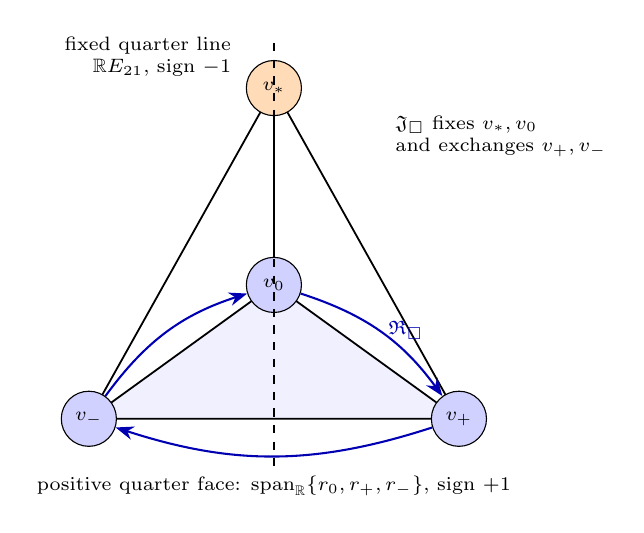
\begin{tikzpicture}[
  scale=1.0,
  vertex/.style={circle,draw=black,fill=white,minimum size=7mm,
                 inner sep=0pt,font=\scriptsize},
  apex/.style={vertex,fill=orange!28},
  facevertex/.style={vertex,fill=blue!18},
  action/.style={-{Stealth[length=2.3mm]},line width=0.75pt},
  edge/.style={line width=0.65pt}
]
\coordinate (A)  at (0,3.05);
\coordinate (B0) at (0,0.55);
\coordinate (Bp) at (2.35,-1.15);
\coordinate (Bm) at (-2.35,-1.15);

\fill[blue!6] (B0)--(Bp)--(Bm)--cycle;
\draw[edge] (B0)--(Bp)--(Bm)--cycle;
\draw[edge] (A)--(B0);
\draw[edge] (A)--(Bp);
\draw[edge] (A)--(Bm);

\node[apex]      (NA)  at (A)  {$v_\ast$};
\node[facevertex](N0)  at (B0) {$v_0$};
\node[facevertex](Np)  at (Bp) {$v_+$};
\node[facevertex](Nm)  at (Bm) {$v_-$};

\draw[action,blue!70!black,bend left=18]
  (N0) to node[pos=0.48,right,font=\scriptsize] {$\mathfrak R_\square$} (Np);
\draw[action,blue!70!black,bend left=18] (Np) to (Nm);
\draw[action,blue!70!black,bend left=18] (Nm) to (N0);

\draw[dashed,line width=0.7pt] (0,3.62)--(0,-1.75);
\node[font=\scriptsize,align=left,anchor=west] at (1.42,2.44)
  {\(\mathfrak J_\square\) fixes \(v_\ast,v_0\)\\
   and exchanges \(v_+,v_-\)};

\node[font=\scriptsize,align=right,anchor=east] at (-0.42,3.45)
  {fixed quarter line\\\(\mathbb R E_{21}\), sign \(-1\)};
\node[font=\scriptsize,align=center] at (0,-2.0)
  {positive quarter face:
   \(\operatorname{span}_{\mathbb R}\{r_0,r_+,r_-\}\), sign \(+1\)};
\end{tikzpicture}
\caption{Affine tetrahedral realization of the proved Fable action.  The
apex is the unique negative quarter direction and the opposite face consists
of the three Fable rays.  The \(C_3\) generator cycles that face, while the
reflection fixes \(v_0\) and exchanges \(v_+\) with \(v_-\).  The drawing
encodes the exact vertex action; no Euclidean edge-length assertion is used.}
\label{fig:Fable-D3-tetrahedral-realization}
\end{figure}

\begin{computation}[Coordinate check for the two vector figures]
\label{comp:visual-tetrahedral-c6-check}
The script and captured receipt
\[
\begin{gathered}
 \texttt{verification/verify\_visual\_tetrahedral\_and\_c6\_figures.py},\\
 \texttt{verification/verify\_visual\_tetrahedral\_and\_c6\_figures\_output.txt}
\end{gathered}
\]
verify the determinant in
\eqref{eq:Fable-D3-tetrahedral-coordinate-matrix}, all vertex actions in
\eqref{eq:Fable-tetrahedron-C3-action}--%
\eqref{eq:Fable-tetrahedron-C2-action}, the four quarter signs in
\eqref{eq:Fable-tetrahedron-quarter-signs}, and the complete exponent
inversion displayed in \cref{fig:adjacent-c6-origin-inversion}.
\end{computation}

\begin{theorem}[Exact spatial quarter altitude of the transported raw-cell
tetrahedron]
\label{thm:Fable-ES-raw-tetrahedron-quarter-altitude}
Define
\begin{equation}
 \Phi_\triangle
 :=
 A^{-1}\circ\Psi_{\mathrm{circ}}\circ\mathcal T_\square
 \label{eq:Fable-ES-raw-tetrahedron-map}
\end{equation}
from the raw-cell space to the ordered Sarnak coordinates
\((T,X,Y,W)\).  For the four vertices in
\cref{cor:Fable-D3-tetrahedral-realization}, one has
\begin{align}
 z_\ast:=\Phi_\triangle(v_\ast)
 &=\left(\frac34,0,\frac54,0\right),\notag\\
 z_0:=\Phi_\triangle(v_0)
 &=\left(\frac52,2,\frac32,0\right),\notag\\
 z_+:=\Phi_\triangle(v_+)
 &=\left(\frac52,-1,\frac32,\sqrt3\right),\notag\\
 z_-:=\Phi_\triangle(v_-)
 &=\left(\frac52,-1,\frac32,-\sqrt3\right).
 \label{eq:Fable-ES-raw-tetrahedron-vertices}
\end{align}
The apex is spacelike and the opposite face is null:
\begin{equation}
 q_{\mathrm L}(z_\ast)=1,
 \qquad
 q_{\mathrm L}(z_0)
 =q_{\mathrm L}(z_+)
 =q_{\mathrm L}(z_-)=0.
 \label{eq:Fable-ES-raw-tetrahedron-Lorentz-norms}
\end{equation}
Moreover, the complete raw-cell action intertwines with the
Erd\H{o}s--Straus-aligned face action:
\begin{equation}
 \Phi_\triangle\mathfrak R_\square
 =R_{\mathrm{face}}\Phi_\triangle,
 \qquad
 \Phi_\triangle\mathfrak J_\square
 =s_W\Phi_\triangle.
 \label{eq:Fable-ES-raw-tetrahedron-intertwining}
\end{equation}

Let
\[
 \pi_{\mathrm{sp}}(T,X,Y,W)=(X,Y,W),
 \qquad
 p_\ast=\pi_{\mathrm{sp}}(z_\ast),
 \quad
 p_a=\pi_{\mathrm{sp}}(z_a).
\]
The centroid of the opposite face and the apex are
\begin{equation}
 \overline p_{\mathrm{face}}
 :=\frac13(p_0+p_++p_-)
 =\left(0,\frac32,0\right),
 \qquad
 p_\ast=\left(0,\frac54,0\right).
 \label{eq:Fable-ES-raw-tetrahedron-centroid-apex}
\end{equation}
Consequently,
\begin{equation}
 \overline p_{\mathrm{face}}-p_\ast
 =\left(0,\frac14,0\right).
 \label{eq:Fable-ES-raw-tetrahedron-quarter-altitude}
\end{equation}
The Euclidean metric data of this spatial tetrahedron are
\begin{align}
 \lVert p_a-p_b\rVert&=2\sqrt3
 &&(a\ne b,\ a,b\in\{0,+,-\}),\notag\\
 \lVert p_\ast-p_a\rVert&=\frac{\sqrt{65}}4
 &&(a\in\{0,+,-\}),\notag\\
 \operatorname{Vol}
 \operatorname{conv}\{p_\ast,p_0,p_+,p_-\}
 &=\frac{\sqrt3}{4}.
 \label{eq:Fable-ES-raw-tetrahedron-metric-data}
\end{align}
Thus the unique negative-quarter raw cell is the fixed spatial apex,
the three positive-quarter rays are its null opposite face, and the exact
face-to-apex altitude is \(1/4\).  This is the raw-cell coordinate
realization of the tetrahedral quarter in
\cref{thm:time-colour-quarter-altitude}.  The
Erd\H{o}s--Straus input for the four vertices in
\eqref{eq:Fable-ES-raw-tetrahedron-vertices} is exactly the proved
alignment of the face reflection with denominator exchange \(s_W\).
The later arithmetic intertwiner
\cref{thm:exceptional-C4-Fable-tetrahedron-intertwiner} realizes these same
four vertices as the exceptional \(C_4\) quotient: its missing antipode is
\(v_\ast\), its three supported classes have equal mass on the opposite
face, and their arithmetic barycentre gives the displacement in
\eqref{eq:Fable-ES-raw-tetrahedron-quarter-altitude}.
The later order-eight calculation
\cref{thm:order-eight-support-eight-cell-intertwiner} shows that the
six-supported \(C_8\) and \(C_4\times C_2\) extrema consist of two such
three-cell faces, with their two missing classes occupying the two fixed
apex cells of the crossed eight-cell carrier.
\end{theorem}

\begin{proof}
Apply \(\mathcal T_\square\) from
\eqref{eq:four-cell-explicit-quarter-images} to
\(v_\ast=E_{21}\) and to the three raw vectors in
\eqref{eq:Fable-null-rays-raw-cell-preimages}.  The results are respectively
\[
 \left(2,0,0,-\frac12\right),
 \qquad
 (4,0,2,1),
 \qquad
 (4,\sqrt3,-1,1),
 \qquad
 (4,-\sqrt3,-1,1).
\]
Applying the Sarnak map
\eqref{eq:circle-Sarnak-coordinates} and then
\(A^{-1}(T,X,Y,W)=(T,Y,W,X)\) gives
\eqref{eq:Fable-ES-raw-tetrahedron-vertices}.  Direct substitution into
\(q_{\mathrm L}=X^2+Y^2+W^2-T^2\) proves
\eqref{eq:Fable-ES-raw-tetrahedron-Lorentz-norms}.

By definition of the pulled-back raw-cell generators,
\[
 \mathcal T_\square\mathfrak R_\square
 =R_{XY}\mathcal T_\square,
 \qquad
 \mathcal T_\square\mathfrak J_\square
 =s_X\mathcal T_\square.
\]
The coefficient rotations commute with
\(\Psi_{\mathrm{circ}}\), and conjugation by \(A^{-1}\) gives
\eqref{eq:Fable-face-ES-transport-matrices}.  This proves
\eqref{eq:Fable-ES-raw-tetrahedron-intertwining}.

Spatial projection of
\eqref{eq:Fable-ES-raw-tetrahedron-vertices} gives
\[
 p_\ast=\left(0,\frac54,0\right),
 \quad
 p_0=\left(2,\frac32,0\right),
 \quad
 p_+=\left(-1,\frac32,\sqrt3\right),
 \quad
 p_-=\left(-1,\frac32,-\sqrt3\right).
\]
Their average proves
\eqref{eq:Fable-ES-raw-tetrahedron-centroid-apex} and
\eqref{eq:Fable-ES-raw-tetrahedron-quarter-altitude}.  Direct squared
distances give \(12\) on every face edge and \(65/16\) on every apex
edge.  Finally,
\[
 \frac16
 \left|
 \det
 \begin{pmatrix}
  p_0-p_\ast&p_+-p_\ast&p_--p_\ast
 \end{pmatrix}
 \right|
 =\frac{\sqrt3}{4},
\]
which proves \eqref{eq:Fable-ES-raw-tetrahedron-metric-data}.
\end{proof}

\begin{theorem}[Affine Lorentz spectrum and exact axial origin of the
spatial quarter]
\label{thm:Fable-ES-affine-Lorentz-spectrum}
Equip the raw-cell space with the Euclidean inner product for which
\((E_{11},E_{12},E_{21},E_{22})\) is an orthonormal basis, and let
\(\eta_{\mathrm L}=\operatorname{diag}(-1,1,1,1)\) in the ordered Sarnak
coordinates \((T,X,Y,W)\).  The matrix of \(\Phi_\triangle\) is
\begin{equation}
 [\Phi_\triangle]
 =
 \begin{pmatrix}
  \frac58&0&\frac34&\frac58\\
  0&1&0&0\\
  \frac38&0&\frac54&\frac38\\
  \frac12&0&0&-\frac12
 \end{pmatrix},
 \qquad
 \det\Phi_\triangle=-\frac12.
 \label{eq:Fable-ES-full-transport-matrix}
\end{equation}
Put
\begin{align*}
 \mathsf E_{\mathrm{raw}}
 &:=[v_0-v_\ast\ \ v_+-v_\ast\ \ v_--v_\ast],\\
 \mathsf E_{\mathrm L}
 &:=[z_0-z_\ast\ \ z_+-z_\ast\ \ z_--z_\ast],\\
 \mathsf E_{\mathrm{sp}}
 &:=[p_0-p_\ast\ \ p_+-p_\ast\ \ p_--p_\ast]
\end{align*}
and define the three Gram matrices
\begin{equation}
 G_{\mathrm{raw}}=\mathsf E_{\mathrm{raw}}^{\mathsf T}
                    \mathsf E_{\mathrm{raw}},
 \quad
 G_{\mathrm L}=\mathsf E_{\mathrm L}^{\mathsf T}\eta_{\mathrm L}
                    \mathsf E_{\mathrm L},
 \quad
 G_{\mathrm{sp}}=\mathsf E_{\mathrm{sp}}^{\mathsf T}
                    \mathsf E_{\mathrm{sp}}.
 \label{eq:Fable-ES-three-affine-Gram-matrices}
\end{equation}
They are
\begin{equation}
 G_{\mathrm{raw}}
 =\begin{pmatrix}13&7&7\\7&16&4\\7&4&16\end{pmatrix},
 \quad
 G_{\mathrm L}
 =\begin{pmatrix}1&-5&-5\\-5&1&-5\\-5&-5&1\end{pmatrix},
 \quad
 G_{\mathrm{sp}}
 =\frac1{16}
  \begin{pmatrix}65&-31&-31\\-31&65&-31\\-31&-31&65\end{pmatrix}.
 \label{eq:Fable-ES-affine-Gram-matrices-explicit}
\end{equation}
Their two generalized characteristic polynomials factor as
\begin{align}
 \det(G_{\mathrm L}-\lambda G_{\mathrm{raw}})
 &=-324(\lambda-1)(2\lambda-1)(3\lambda+1),
 \label{eq:Fable-ES-Lorentz-generalized-spectrum}\\
 \det(G_{\mathrm{sp}}-\lambda G_{\mathrm{raw}})
 &=-\frac{27}{4}(\lambda-1)(2\lambda-1)(144\lambda-1).
 \label{eq:Fable-ES-spatial-generalized-spectrum}
\end{align}
The same three coefficient directions diagonalize both pairs:
\begin{equation}
 u_X=(-2,1,1)^{\mathsf T},
 \qquad
 u_W=(0,-1,1)^{\mathsf T},
 \qquad
 u_{\mathrm{ax}}=(1,1,1)^{\mathsf T}.
 \label{eq:Fable-ES-affine-three-directions}
\end{equation}
Their generalized values are respectively
\begin{equation}
 \begin{array}{c|ccc}
  &u_X&u_W&u_{\mathrm{ax}}\\ \hline
  (G_{\mathrm L},G_{\mathrm{raw}})&1&\frac12&-\frac13\\[2pt]
  (G_{\mathrm{sp}},G_{\mathrm{raw}})&1&\frac12&\frac1{144}
 \end{array}.
 \label{eq:Fable-ES-affine-three-generalized-values}
\end{equation}
Thus the Lorentz form on the transported affine tangent space has signature
\((2,1)\).  The spatial transport has exact length factors
\begin{equation}
 1,
 \qquad
 \frac1{\sqrt2},
 \qquad
 \frac1{12}.
 \label{eq:Fable-ES-spatial-length-factors}
\end{equation}
The last factor is the one-dimensional face-centroid axis.  More precisely,
\begin{equation}
 \frac13\mathsf E_{\mathrm{raw}}u_{\mathrm{ax}}
 =2E_{11}-E_{21}+2E_{22},
 \qquad
 \frac13\mathsf E_{\mathrm{sp}}u_{\mathrm{ax}}
 =\left(0,\frac14,0\right).
 \label{eq:Fable-ES-raw-axis-to-quarter-axis}
\end{equation}
The raw vector on the left has length (3), so the quarter altitude is
exactly its image under the unique axial length factor (1/12).

Finally, the raw and spatial affine volumes and their exact ratio are
\begin{equation}
 \operatorname{Vol}_{\mathrm{raw}}=3\sqrt6,
 \qquad
 \operatorname{Vol}_{\mathrm{sp}}=\frac{\sqrt3}{4},
 \qquad
 \frac{\operatorname{Vol}_{\mathrm{sp}}}
      {\operatorname{Vol}_{\mathrm{raw}}}
 =\frac{\sqrt2}{24}.
 \label{eq:Fable-ES-affine-volume-factor}
\end{equation}
\end{theorem}

\begin{proof}
Multiplication of the three matrices in
\eqref{eq:Fable-ES-raw-tetrahedron-map} gives
\eqref{eq:Fable-ES-full-transport-matrix}.  Substitution of the four raw
vertices and their transported spatial coordinates gives the three matrices
in \eqref{eq:Fable-ES-affine-Gram-matrices-explicit}.  Direct determinants
give \eqref{eq:Fable-ES-Lorentz-generalized-spectrum} and
\eqref{eq:Fable-ES-spatial-generalized-spectrum}.

For each vector in \eqref{eq:Fable-ES-affine-three-directions}, direct
multiplication proves the corresponding generalized eigenvalue in
\eqref{eq:Fable-ES-affine-three-generalized-values}.  In particular,
\begin{align*}
 \mathsf E_{\mathrm{raw}}u_X&=-6E_{12},&
 \mathsf E_{\mathrm{sp}}u_X&=(-6,0,0),\\
 \mathsf E_{\mathrm{raw}}u_W&=2\sqrt3(-E_{11}+E_{22}),&
 \mathsf E_{\mathrm{sp}}u_W&=(0,0,-2\sqrt3).
\end{align*}
The equal coefficients of \(u_{\mathrm{ax}}\) make it the fixed axis of the
face permutation, and its third generalized spatial value is distinct from
the other two.  This proves both its one-dimensionality and
\eqref{eq:Fable-ES-raw-axis-to-quarter-axis}.

Lastly,
\[
 \det G_{\mathrm{raw}}=1944,
 \qquad
 \det G_{\mathrm{sp}}=\frac{27}{4}.
\]
Taking the square root and dividing by (3!=6) gives the two volumes in
\eqref{eq:Fable-ES-affine-volume-factor}; their quotient is
\(\sqrt2/24\).
\end{proof}

\begin{corollary}[Exact affine-invariant geodesic length--volume identity]
\label{cor:Fable-ES-affine-complexity-volume}
Let
\[
 V_{\mathrm{aff}}:=\operatorname{im}\mathsf E_{\mathrm{raw}}
\]
carry the raw Euclidean inner product, and define the spatial transport
\[
 L_{\mathrm{sp}}\colon V_{\mathrm{aff}}\longrightarrow\mathbb R^3,
 \qquad
 L_{\mathrm{sp}}(\mathsf E_{\mathrm{raw}}u)
 :=\mathsf E_{\mathrm{sp}}u.
\]
Write \(L_{\mathrm{sp}}=UP\) for its polar decomposition.  Thus
\[
 P=(L_{\mathrm{sp}}^*L_{\mathrm{sp}})^{1/2}
 \in\operatorname{Sym}^+(V_{\mathrm{aff}}).
\]
For the affine-invariant metric
\begin{equation}
 g_Q(H,K)
 :=\operatorname{tr}(Q^{-1}H\,Q^{-1}K)
 \qquad
 \bigl(Q\in\operatorname{Sym}^+(V_{\mathrm{aff}})\bigr),
 \label{eq:Fable-ES-SPD-affine-metric}
\end{equation}
let \(\mathcal C_{\mathrm{aff}}\) be the geodesic length from \(I\) to
\(P\), and put
\[
 J_{\mathrm{vol}}:=|\det L_{\mathrm{sp}}|=\det P.
\]
Then
\begin{align}
 \operatorname{Spec}(P)
 &=\left\{1,\frac1{\sqrt2},\frac1{12}\right\},
 \label{eq:Fable-ES-positive-polar-spectrum}\\
 \mathcal C_{\mathrm{aff}}^2
 &=(\log12)^2+\frac14(\log2)^2,
 \qquad
 J_{\mathrm{vol}}=\frac1{12\sqrt2}=\frac{\sqrt2}{24},
 \label{eq:Fable-ES-affine-complexity-and-volume}\\
 2\mathcal C_{\mathrm{aff}}^2
 &=\left(\log J_{\mathrm{vol}}^{-1}\right)^2
   +\left(\log(6\sqrt2)\right)^2.
 \label{eq:Fable-ES-affine-complexity-volume-identity}
\end{align}
\end{corollary}

\begin{proof}
The spatial generalized eigenvalues in
\eqref{eq:Fable-ES-affine-three-generalized-values} are the eigenvalues of
\(L_{\mathrm{sp}}^*L_{\mathrm{sp}}\).  Their positive square roots prove
\eqref{eq:Fable-ES-positive-polar-spectrum}.  For the metric
\eqref{eq:Fable-ES-SPD-affine-metric}, the geodesic from \(I\) to \(P\) is
\[
 \Gamma(t)=\exp(t\log P),\qquad 0\leq t\leq1,
\]
and its length is
\(\|\log P\|_{\mathrm{HS}}\)
\cite{PennecFillardAyache2006}.  The three eigenvalues in
\eqref{eq:Fable-ES-positive-polar-spectrum} therefore give
\[
 \mathcal C_{\mathrm{aff}}^2
 =0^2+\left(-\frac12\log2\right)^2+(-\log12)^2.
\]
Their product gives \(J_{\mathrm{vol}}=1/(12\sqrt2)\), agreeing with
\eqref{eq:Fable-ES-affine-volume-factor}.

Set \(a=\log12\) and \(b=\frac12\log2\).  Then
\[
 \mathcal C_{\mathrm{aff}}^2=a^2+b^2,\qquad
 \log J_{\mathrm{vol}}^{-1}=a+b,\qquad
 a-b=\log(6\sqrt2).
\]
The identity
\[
 2(a^2+b^2)=(a+b)^2+(a-b)^2
\]
proves \eqref{eq:Fable-ES-affine-complexity-volume-identity}.
\end{proof}

\begin{proposition}[Trace--anisotropy decomposition of affine geodesic length]
\label{prop:SPD-trace-anisotropy-decomposition}
Let \(d\geq2\), let \(P\in\operatorname{Sym}^+(d)\), and equip
\(\operatorname{Sym}^+(d)\) with the affine-invariant metric
\[
 g_Q(H,K)=\operatorname{tr}(Q^{-1}H\,Q^{-1}K).
\]
Put
\[
 \mathcal C(P):=d_g(I,P),
 \qquad
 J(P):=\det P,
 \qquad
 X_0:=\log P-\frac{\log J(P)}{d}I.
\]
Then
\begin{equation}
 \mathcal C(P)^2
 =\frac1d\bigl(\log J(P)\bigr)^2+\|X_0\|_{\mathrm{HS}}^2.
 \label{eq:SPD-trace-anisotropy-decomposition}
\end{equation}
For the Fable-to-Sarnak spatial carrier,
\begin{equation}
 \|X_0\|_{\mathrm{HS}}^2
 =\frac16\left(\log(12\sqrt2)\right)^2
  +\frac12\left(\log(6\sqrt2)\right)^2.
 \label{eq:Fable-ES-exact-traceless-anisotropy}
\end{equation}
\end{proposition}

\begin{proof}
Set \(X=\log P\) and
\(\mu=d^{-1}\operatorname{tr}X\).  Since \(P\) is positive definite,
\[
 \operatorname{tr}X=\log\det P=\log J(P).
\]
Moreover \(X=X_0+\mu I\), \(\operatorname{tr}X_0=0\), and hence
\[
 \langle X_0,\mu I\rangle_{\mathrm{HS}}
 =\mu\operatorname{tr}X_0=0,
 \qquad
 \|\mu I\|_{\mathrm{HS}}^2=d\mu^2.
\]
The affine-invariant distance formula
\(\mathcal C(P)=\|\log P\|_{\mathrm{HS}}\) now gives
\eqref{eq:SPD-trace-anisotropy-decomposition}.

For the spatial carrier, put
\[
 s=\log(12\sqrt2),
 \qquad
 r=\log(6\sqrt2).
\]
The proof of
\cref{cor:Fable-ES-affine-complexity-volume} gives
\[
 \mathcal C_{\mathrm{aff}}^2=\frac12(s^2+r^2),
 \qquad
 \log J_{\mathrm{vol}}=-s.
\]
Substitution into
\eqref{eq:SPD-trace-anisotropy-decomposition} with \(d=3\) yields
\[
 \|X_0\|_{\mathrm{HS}}^2
 =\frac12(s^2+r^2)-\frac13s^2
 =\frac16s^2+\frac12r^2,
\]
which is \eqref{eq:Fable-ES-exact-traceless-anisotropy}.
\end{proof}

\begin{corollary}[Sharp logarithmic volume bound]
\label{cor:SPD-sharp-log-volume-bound}
Under the conditions of
\cref{prop:SPD-trace-anisotropy-decomposition},
\begin{equation}
 \mathcal C(P)
 \geq
 \frac{|\log J(P)|}{\sqrt d}.
 \label{eq:SPD-sharp-log-volume-bound}
\end{equation}
Equality holds exactly when
\[
 P=J(P)^{1/d}I.
\]
For the Fable-to-Sarnak spatial carrier the inequality is strict, and its
exact squared gap is
\begin{equation}
 \mathcal C_{\mathrm{aff}}^2
 -\frac13\left(\log J_{\mathrm{vol}}^{-1}\right)^2
 =
 \frac16\left(\log(12\sqrt2)\right)^2
 +\frac12\left(\log(6\sqrt2)\right)^2.
 \label{eq:Fable-ES-sharp-log-volume-gap}
\end{equation}
\end{corollary}

\begin{proof}
Equation
\eqref{eq:SPD-trace-anisotropy-decomposition} is a sum of two
nonnegative squared norms, which proves
\eqref{eq:SPD-sharp-log-volume-bound}.  Equality holds exactly when
\(X_0=0\), equivalently when
\[
 \log P=\frac{\log J(P)}d I.
\]
Exponentiation gives \(P=J(P)^{1/d}I\), and that scalar matrix attains
equality.  The spectrum in
\eqref{eq:Fable-ES-positive-polar-spectrum} contains three distinct
values, so the spatial carrier does not attain equality.  Its squared gap
is \eqref{eq:Fable-ES-exact-traceless-anisotropy}.
\end{proof}

\begin{figure}[htbp]
\centering
\includegraphics[width=\textwidth]
 {figures/fable_es_raw_tetrahedron.pdf}
\caption{\textbf{Exact spatial realization of the transported raw-cell
tetrahedron.}
The left panel plots the true spatial coordinates in
\eqref{eq:Fable-ES-raw-tetrahedron-vertices}: the colored null face lies
at \(Y=3/2\), and the orange spacelike apex lies at \(Y=5/4\).
The black point is the face centroid.  The right panel reads the two
coordinates on their common axis and records the exact altitude, edge
lengths, Euclidean volume, axial length factor, and affine-volume factor.
Every displayed quantity is checked in
\cref{comp:Fable-ES-raw-tetrahedron-check}.}
\label{fig:Fable-ES-raw-tetrahedron-quarter}
\end{figure}

\begin{computation}[Exact check of the transported raw-cell tetrahedron]
\label{comp:Fable-ES-raw-tetrahedron-check}
The generator, checker, and captured receipt
\[
\begin{gathered}
 \texttt{verification/make\_fable\_es\_raw\_tetrahedron\_figure.py},\\
 \texttt{verification/make\_fable\_12289\_count\_orbit\_figure.py},\\
 \texttt{verification/verify\_fable\_es\_raw\_tetrahedron.py},\\
 \texttt{verification/verify\_fable\_es\_raw\_tetrahedron\_output.txt}
\end{gathered}
\]
verify the complete transport map, the four Lorentz norms, both
intertwining identities, the face centroid, the quarter altitude, all six
edge lengths, the spatial volume, all three affine Gram matrices, both
generalized spectra, the three common eigendirections, and the exact
affine-volume factor, positive-polar determinant, quadratic logarithmic
identity, and trace--anisotropy decomposition in
\cref{thm:Fable-ES-raw-tetrahedron-quarter-altitude,%
 thm:Fable-ES-affine-Lorentz-spectrum,%
 cor:Fable-ES-affine-complexity-volume,%
 prop:SPD-trace-anisotropy-decomposition,%
 cor:SPD-sharp-log-volume-bound,%
 thm:Fable-face-12289-count-orbit-identification}.  The maintained
 vector images are
\[
 \texttt{figures/fable\_es\_raw\_tetrahedron.pdf},
 \qquad
 \texttt{figures/fable\_12289\_count\_orbit.pdf}.
\]
\end{computation}

\clearpage
\begin{theorem}[Vertex projection of a centered regular simplex]
\label{thm:regular-simplex-vertex-projection}
Let \(n\geq2\), let \(V\) be a real inner-product space, and suppose
\(v_0,\ldots,v_n\in V\) satisfy
\begin{equation}
 \langle v_i,v_i\rangle=1,
 \qquad
 \langle v_i,v_j\rangle=-\frac1n
 \quad(i\ne j).
 \label{eq:regular-n-simplex-Gram-data}
\end{equation}
Put \(W=\operatorname{span}_{\mathbb R}\{v_0,\ldots,v_n\}\), and let
\(\pi_0\) be the orthogonal projection from \(W\) to
\(W\cap v_0^\perp\).  Then
\begin{equation}
 \sum_{i=0}^{n}v_i=0,
 \qquad
 c_{\mathrm{opp}}
 :=\frac1n\sum_{i=1}^{n}v_i
 =-\frac1n v_0.
 \label{eq:regular-simplex-opposite-centroid}
\end{equation}
For \(1\leq i\leq n\), put \(w_i=\pi_0(v_i)\).  Explicitly,
\begin{equation}
 w_i=v_i+\frac1n v_0,
 \qquad
 \sum_{i=1}^{n}w_i=0,
 \label{eq:regular-simplex-projected-vertices}
\end{equation}
and their Gram matrix is
\begin{equation}
 \langle w_i,w_j\rangle
 =
 \begin{cases}
 \dfrac{n^2-1}{n^2},&i=j,\\[2mm]
 -\dfrac{n+1}{n^2},&i\ne j.
 \end{cases}
 \label{eq:regular-simplex-projected-Gram}
\end{equation}
Consequently,
\begin{equation}
 u_i:=\frac{n}{\sqrt{n^2-1}}\,w_i
 \quad\Longrightarrow\quad
 \langle u_i,u_j\rangle
 =
 \begin{cases}
 1,&i=j,\\[1mm]
 -\dfrac1{n-1},&i\ne j.
 \end{cases}
 \label{eq:regular-simplex-unit-rescaled-face}
\end{equation}
Thus the orthogonal image of the face opposite \(v_0\) is a centered
regular \((n-1)\)-simplex.  The projection erases the single axial
displacement
\begin{equation}
 c_{\mathrm{opp}}-0=-\frac1n v_0.
 \label{eq:regular-simplex-hidden-axial-displacement}
\end{equation}
\end{theorem}

\begin{proof}
Taking the squared norm of the sum of the \(n+1\) vertices gives
\[
 \left\lVert\sum_{i=0}^{n}v_i\right\rVert^2
 =
 (n+1)+n(n+1)\left(-\frac1n\right)=0.
\]
This proves the first identity in
\eqref{eq:regular-simplex-opposite-centroid}; the second follows by
isolating \(v_0\) and dividing by \(n\).

Since \(\langle v_i,v_0\rangle=-1/n\) for \(i\geq1\),
\[
 \pi_0(v_i)
 =
 v_i-\langle v_i,v_0\rangle v_0
 =
 v_i+\frac1n v_0.
\]
Summing these identities and using
\(\sum_{i=1}^{n}v_i=-v_0\) gives
\(\sum_iw_i=0\).  Direct expansion gives
\[
 \langle w_i,w_i\rangle
 =
 1-\frac2{n^2}+\frac1{n^2}
 =
 \frac{n^2-1}{n^2},
\]
and, for \(i\ne j\),
\[
 \langle w_i,w_j\rangle
 =
 -\frac1n-\frac2{n^2}+\frac1{n^2}
 =
 -\frac{n+1}{n^2}.
\]
This proves \eqref{eq:regular-simplex-projected-Gram}.  Multiplication by
\(n/\sqrt{n^2-1}\) sends the off-diagonal entry to
\[
 -\frac{n+1}{n^2-1}=-\frac1{n-1},
\]
which proves \eqref{eq:regular-simplex-unit-rescaled-face}.  Finally,
\(\pi_0(c_{\mathrm{opp}})=0\) because
\(c_{\mathrm{opp}}=-v_0/n\), proving
\eqref{eq:regular-simplex-hidden-axial-displacement}.
\end{proof}

\begin{corollary}[The hidden quarter in the regular \(4\)-simplex]
\label{cor:regular-four-simplex-hidden-quarter}
Under the hypotheses of
\cref{thm:regular-simplex-vertex-projection} with \(n=4\), the face
opposite \(v_0\) is the affine translate
\begin{equation}
 \operatorname{conv}\{v_1,v_2,v_3,v_4\}
 =
 -\frac14v_0+
 \operatorname{conv}\{w_1,w_2,w_3,w_4\}.
 \label{eq:four-simplex-opposite-face-translation}
\end{equation}
Its centroid is \(-v_0/4\), while the centroid of its orthogonal image is
\(0\).  The projected Gram matrix has diagonal entry \(15/16\) and
off-diagonal entry \(-5/16\); multiplication of every \(w_i\) by
\(4/\sqrt{15}\) gives a regular tetrahedron with off-diagonal entry
\(-1/3\).

Every permutation of \(v_1,v_2,v_3,v_4\) extends to an orthogonal
transformation of \(W\) fixing \(v_0\).  The point \(-v_0/4\) is the unique
point of the opposite affine face fixed by all these permutations.
Therefore the signed quarter displacement is intrinsic to the
vertex-stabilized projection.
\end{corollary}

\begin{proof}
Equations
\eqref{eq:four-simplex-opposite-face-translation} and the two Gram entries
are the case \(n=4\) of
\eqref{eq:regular-simplex-projected-vertices}--%
\eqref{eq:regular-simplex-projected-Gram}.  A permutation of the four
opposite vertices preserves every entry of
\eqref{eq:regular-n-simplex-Gram-data}, hence induces an orthogonal
transformation on \(W\) fixing \(v_0\).  A point of the opposite affine
face fixed by every permutation must have four equal barycentric
coordinates.  Their sum is one, so each equals \(1/4\); the fixed point is
the centroid \(-v_0/4\).
\end{proof}

\begin{theorem}[Exact rank--volume identities for centered regular simplices]
\label{thm:regular-simplex-rank-volume}
Retain the hypotheses and notation of
\cref{thm:regular-simplex-vertex-projection}.  Let
\[
 C_n:=\bigl(\langle v_i,v_j\rangle\bigr)_{0\leq i,j\leq n},
 \qquad
 W_n:=\bigl(\langle w_i,w_j\rangle\bigr)_{1\leq i,j\leq n},
\]
and let \(\operatorname{pdet}\) denote the product of the nonzero
eigenvalues.  If \(\mathbf 1_m\) is the all-one column of length \(m\),
then
\begin{align}
 C_n
 &=
 \frac{n+1}{n}I_{n+1}
 -\frac1n\mathbf 1_{n+1}\mathbf 1_{n+1}^{\mathsf T},
 &
 \operatorname{Spec}(C_n)
 &=
 \left\{0^{[1]},
 \left(\frac{n+1}{n}\right)^{[n]}\right\},
 \label{eq:regular-simplex-centered-Gram-spectrum}\\
 W_n
 &=
 \frac{n+1}{n}
 \left(
 I_n-\frac1n\mathbf 1_n\mathbf 1_n^{\mathsf T}
 \right),
 &
 \operatorname{Spec}(W_n)
 &=
 \left\{0^{[1]},
 \left(\frac{n+1}{n}\right)^{[n-1]}\right\}.
 \label{eq:regular-simplex-face-Gram-spectrum}
\end{align}
Consequently,
\begin{equation}
 \operatorname{rank}C_n=n,
 \qquad
 \operatorname{rank}W_n=n-1,
 \qquad
 \operatorname{pdet}C_n
 =
 \frac{n+1}{n}\operatorname{pdet}W_n.
 \label{eq:regular-simplex-pdet-rank-step}
\end{equation}

Let \(\mathcal V_n\) be the Euclidean \(n\)-volume of
\(\operatorname{conv}\{v_0,\ldots,v_n\}\), and let
\(\mathcal A_{n-1}\) be the Euclidean \((n-1)\)-volume of its face
opposite \(v_0\).  Then
\begin{align}
 \mathcal V_n^2
 &=
 \frac{n+1}{(n!)^2}\operatorname{pdet}C_n
 =
 \frac{(n+1)^{n+1}}{(n!)^2n^n},
 \label{eq:regular-simplex-full-volume-pdet}\\
 \mathcal A_{n-1}^2
 &=
 \frac{n}{((n-1)!)^2}\operatorname{pdet}W_n
 =
 \frac{(n+1)^{n-1}}
 {n^{n-2}((n-1)!)^2}.
 \label{eq:regular-simplex-face-volume-pdet}
\end{align}
The altitude from \(v_0\) to the opposite face is
\begin{equation}
 h_n
 =
 \left\lVert v_0-c_{\mathrm{opp}}\right\rVert
 =
 \frac{n+1}{n},
 \qquad
 \mathcal V_n=\frac{h_n}{n}\mathcal A_{n-1}.
 \label{eq:regular-simplex-altitude-volume}
\end{equation}
Thus the loss of one Gram rank under vertex projection, the factor
\((n+1)/n\) between the two pseudodeterminants, and the hidden axial
displacement \(1/n\) are exact parts of one dimension--volume identity.

For \(n=4\), these identities give
\begin{equation}
 \operatorname{pdet}C_4=\frac{625}{256},
 \qquad
 \operatorname{pdet}W_4=\frac{125}{64},
 \qquad
 \mathcal V_4^2=\frac{3125}{147456},
 \qquad
 \mathcal A_3^2=\frac{125}{576},
 \qquad
 h_4=\frac54.
 \label{eq:regular-four-simplex-rank-volume-data}
\end{equation}
\end{theorem}

\begin{proof}
Equations
\eqref{eq:regular-simplex-centered-Gram-spectrum} and
\eqref{eq:regular-simplex-face-Gram-spectrum} follow directly from
\eqref{eq:regular-n-simplex-Gram-data} and
\eqref{eq:regular-simplex-projected-Gram}.  The matrix
\(\mathbf 1_m\mathbf 1_m^{\mathsf T}\) has eigenvalue \(m\) on the
all-one line and eigenvalue \(0\) on its orthogonal complement.  The two
displayed spectra and \eqref{eq:regular-simplex-pdet-rank-step} follow.

For \(1\leq i\leq n\), put \(e_i=v_i-v_0\).  Their edge Gram matrix is
\begin{equation}
 \bigl(\langle e_i,e_j\rangle\bigr)_{1\leq i,j\leq n}
 =
 \frac{n+1}{n}
 \left(I_n+\mathbf 1_n\mathbf 1_n^{\mathsf T}\right).
 \label{eq:regular-simplex-edge-Gram}
\end{equation}
The second factor has eigenvalue \(n+1\) on the all-one line and
eigenvalue \(1\) with multiplicity \(n-1\).  Hence
\[
 \det\bigl(\langle e_i,e_j\rangle\bigr)
 =
 (n+1)\left(\frac{n+1}{n}\right)^n.
\]
The Gram determinant formula for simplex volume now gives
\[
 (n!)^2\mathcal V_n^2
 =
 (n+1)\operatorname{pdet}C_n,
\]
which is \eqref{eq:regular-simplex-full-volume-pdet}.

Using \(v_n\) as a base point of the opposite face, the \(n-1\) edge
vectors \(v_i-v_n\), \(1\leq i\leq n-1\), have Gram matrix
\[
 \frac{n+1}{n}
 \left(
 I_{n-1}+\mathbf 1_{n-1}\mathbf 1_{n-1}^{\mathsf T}
 \right).
\]
Its determinant is
\[
 n\left(\frac{n+1}{n}\right)^{n-1}
 =
 n\operatorname{pdet}W_n.
\]
The \((n-1)\)-dimensional Gram determinant formula proves
\eqref{eq:regular-simplex-face-volume-pdet}.

Finally,
\[
 v_0-c_{\mathrm{opp}}
 =
 \left(1+\frac1n\right)v_0,
\]
so \(h_n=(n+1)/n\).  The pyramid formula
\(\mathcal V_n=h_n\mathcal A_{n-1}/n\) proves
\eqref{eq:regular-simplex-altitude-volume}.  Substitution of \(n=4\)
gives \eqref{eq:regular-four-simplex-rank-volume-data}.
\end{proof}

\begin{corollary}[Trace-one simplex states and exact entropy--volume identities]
\label{cor:regular-simplex-entropy-volume}
Define
\begin{equation}
 \rho_n
 :=
 \frac{C_n}{\operatorname{tr}C_n}
 =
 \frac1n
 \left(
 I_{n+1}
 -\frac1{n+1}
 \mathbf 1_{n+1}\mathbf 1_{n+1}^{\mathsf T}
 \right),
 \label{eq:regular-simplex-vertex-state}
\end{equation}
and
\begin{equation}
 \sigma_{n-1}
 :=
 \frac{W_n}{\operatorname{tr}W_n}
 =
 \frac1{n-1}
 \left(
 I_n-\frac1n\mathbf 1_n\mathbf 1_n^{\mathsf T}
 \right).
 \label{eq:regular-simplex-face-state}
\end{equation}
These are positive semidefinite trace-one matrices with
\begin{align}
 \operatorname{Spec}(\rho_n)
 &=
 \left\{0^{[1]},\left(\frac1n\right)^{[n]}\right\},
 &
 \operatorname{tr}(\rho_n^2)
 &=
 \frac1n,
 &
 S(\rho_n)
 &:=-\operatorname{tr}(\rho_n\log\rho_n)=\log n,
 \label{eq:regular-simplex-vertex-state-data}\\
 \operatorname{Spec}(\sigma_{n-1})
 &=
 \left\{0^{[1]},
 \left(\frac1{n-1}\right)^{[n-1]}\right\},
 &
 \operatorname{tr}(\sigma_{n-1}^2)
 &=
 \frac1{n-1},
 &
 S(\sigma_{n-1})
 &=\log(n-1).
 \label{eq:regular-simplex-face-state-data}
\end{align}
Here \(0\log0\) is interpreted by continuity as \(0\).

The Euclidean volumes are recovered from the support determinants of these
two states:
\begin{align}
 \mathcal V_n^2
 &=
 \frac{(n+1)^{n+1}}{(n!)^2}
 \operatorname{pdet}\rho_n,
 &
 \operatorname{pdet}\rho_n
 &=
 n^{-n},
 \label{eq:regular-simplex-vertex-state-volume}\\
 \mathcal A_{n-1}^2
 &=
 \frac{(n^2-1)^{n-1}}
 {n^{n-2}((n-1)!)^2}
 \operatorname{pdet}\sigma_{n-1},
 &
 \operatorname{pdet}\sigma_{n-1}
 &=
 (n-1)^{-(n-1)}.
 \label{eq:regular-simplex-face-state-volume}
\end{align}
Equivalently,
\begin{align}
 \log\mathcal V_n^2
 &=
 (n+1)\log(n+1)-2\log(n!)
 -nS(\rho_n),
 \label{eq:regular-simplex-vertex-entropy-volume}\\
 \log\mathcal A_{n-1}^2
 &=
 (n-1)\log(n^2-1)-(n-2)\log n
 -2\log((n-1)!)
 -(n-1)S(\sigma_{n-1}).
 \label{eq:regular-simplex-face-entropy-volume}
\end{align}
For \(n=4\), the four nonzero eigenvalues of \(\rho_4\) are all \(1/4\).
Their common value equals the magnitude of the directed centroid
displacement in
\eqref{eq:regular-simplex-hidden-axial-displacement} and
\eqref{eq:Fable-regular-four-simplex-centroid}.
\end{corollary}

\begin{proof}
The trace of \(C_n\) is \(n+1\), while
\[
 \operatorname{tr}W_n
 =
 n\frac{n^2-1}{n^2}
 =
 \frac{n^2-1}{n}.
\]
Dividing
\eqref{eq:regular-simplex-centered-Gram-spectrum} and
\eqref{eq:regular-simplex-face-Gram-spectrum} by these trace values gives
\eqref{eq:regular-simplex-vertex-state-data} and
\eqref{eq:regular-simplex-face-state-data}.  The purity, entropy, and
pseudodeterminant formulas follow by summing or multiplying the nonzero
eigenvalues.  Substitution in
\eqref{eq:regular-simplex-full-volume-pdet} and
\eqref{eq:regular-simplex-face-volume-pdet} proves
\eqref{eq:regular-simplex-vertex-state-volume} and
\eqref{eq:regular-simplex-face-state-volume}.  Taking logarithms and using
the two entropy identities proves
\eqref{eq:regular-simplex-vertex-entropy-volume} and
\eqref{eq:regular-simplex-face-entropy-volume}.  The case \(n=4\) follows
from \eqref{eq:regular-simplex-vertex-state-data}.
\end{proof}

\begin{corollary}[Exact Hilbert--Schmidt control-length--volume carrier]
\label{cor:regular-simplex-control-length-volume}
Let
\[
 P_n
 :=
 I_{n+1}
 -\frac1{n+1}\mathbf 1_{n+1}\mathbf 1_{n+1}^{\mathsf T}
 =
 n\rho_n
\]
be the orthogonal projection onto the support of \(\rho_n\), and put
\begin{equation}
 K_n
 :=
 P_n-\frac{n}{n+1}I_{n+1}.
 \label{eq:regular-simplex-traceless-generator}
\end{equation}
For a Hermitian control \(H\), define the Hilbert--Schmidt cost
\[
 F_{\mathrm{HS}}(H):=\sqrt{\operatorname{tr}(H^2)}.
\]
This cost is bi-invariant.  Consider the two paths
\begin{equation}
 \gamma_n^\rho(t):=\exp(-it\rho_n)\in U(n+1),
 \qquad
 \gamma_n^0(t):=\exp(-itK_n)\in SU(n+1),
 \qquad 0\leq t\leq1.
 \label{eq:regular-simplex-two-control-paths}
\end{equation}
Their exact lengths are
\begin{equation}
 \mathcal L_\rho(n)
 :=
 L_{F_{\mathrm{HS}}}(\gamma_n^\rho)
 =
 \frac1{\sqrt n},
 \qquad
 \mathcal L_0(n)
 :=
 L_{F_{\mathrm{HS}}}(\gamma_n^0)
 =
 \sqrt{\frac{n}{n+1}}.
 \label{eq:regular-simplex-control-lengths}
\end{equation}
The hidden axial displacement, state purity, and squared first control
length coincide:
\begin{equation}
 \left\lVert c_{\mathrm{opp}}\right\rVert
 =
 \operatorname{tr}(\rho_n^2)
 =
 \mathcal L_\rho(n)^2
 =
 \frac1n.
 \label{eq:regular-simplex-displacement-purity-length}
\end{equation}
The full simplex volume has the two exact control-length expressions
\begin{equation}
 \boxed{
 \mathcal V_n^2
 =
 \frac{(n+1)^{n+1}}{(n!)^2}
 \mathcal L_\rho(n)^{2n}
 =
 \frac{n+1}{(n!)^2}
 \mathcal L_0(n)^{-2n}.}
 \label{eq:regular-simplex-control-length-volume}
\end{equation}
These paths are fully specified instances of the geometric control
length used in Nielsen's circuit geometry
\cite{Nielsen2005,NielsenEtAl2006}.

For \(n=4\),
\begin{equation}
 \mathcal L_\rho(4)=\frac12,
 \qquad
 \mathcal L_0(4)=\frac2{\sqrt5},
 \qquad
 \mathcal V_4^2
 =
 \frac{5^5}{(4!)^2}\left(\frac12\right)^8
 =
 \frac5{(4!)^2}\left(\frac2{\sqrt5}\right)^{-8}.
 \label{eq:regular-four-simplex-control-length-volume}
\end{equation}
\end{corollary}

\begin{proof}
For a unitary \(Q\),
\[
 \operatorname{tr}\bigl((QHQ^\ast)^2\bigr)
 =
 \operatorname{tr}(QH^2Q^\ast)
 =
 \operatorname{tr}(H^2),
\]
which proves bi-invariance.  Both paths in
\eqref{eq:regular-simplex-two-control-paths} have constant adapted
Hamiltonians, respectively \(\rho_n\) and \(K_n\).  Therefore their lengths
are the Hilbert--Schmidt norms of those two matrices.

The projection \(P_n\) has rank and trace \(n\).  Since
\(\rho_n=P_n/n\),
\[
 \operatorname{tr}(\rho_n^2)
 =
 \frac1{n^2}\operatorname{tr}(P_n)
 =
 \frac1n.
\]
Equation \eqref{eq:regular-simplex-opposite-centroid} gives
\(\lVert c_{\mathrm{opp}}\rVert=1/n\), proving
\eqref{eq:regular-simplex-displacement-purity-length}.

On the range of \(P_n\), the eigenvalue of \(K_n\) is \(1/(n+1)\);
on its kernel, the eigenvalue is \(-n/(n+1)\).  Thus
\[
 \operatorname{tr}(K_n)=0,
 \qquad
 \operatorname{tr}(K_n^2)
 =
 n\frac1{(n+1)^2}
 +\frac{n^2}{(n+1)^2}
 =
 \frac{n}{n+1}.
\]
This proves \eqref{eq:regular-simplex-control-lengths} and also shows that
\(\gamma_n^0(t)\) lies in \(SU(n+1)\).
Substitution of the two squared lengths into
\eqref{eq:regular-simplex-full-volume-pdet} proves
\eqref{eq:regular-simplex-control-length-volume}; the case \(n=4\) is
\eqref{eq:regular-four-simplex-control-length-volume}.
\end{proof}

\begin{theorem}[Finite Tomita sector carried by regular-simplex support]
\label{thm:regular-simplex-finite-Tomita-sector}
Let \(V_n\) be the complexification of the real span of the centered
regular-simplex vertices in
\cref{thm:regular-simplex-vertex-projection}, and let
\[
 \mathsf S_n:\mathbb C^{n+1}\longrightarrow V_n,
 \qquad
 \mathsf S_ne_i=v_i
\]
be the synthesis map.  Then
\begin{equation}
 \mathsf S_n^\ast\mathsf S_n=C_n,
 \qquad
 \ker\mathsf S_n
 =
 \mathbb C\mathbf 1_{n+1},
 \qquad
 P_n
 =
 I_{n+1}
 -\frac1{n+1}\mathbf 1_{n+1}\mathbf 1_{n+1}^{\mathsf T}
 \label{eq:regular-simplex-synthesis-support}
\end{equation}
is the support projection of \(C_n\) and \(\rho_n\).

Define the support corner and its Hilbert--Schmidt standard space by
\begin{equation}
 \mathcal A_n
 :=
 P_nM_{n+1}(\mathbb C)P_n,
 \qquad
 \mathscr H_n
 :=
 \bigl(\mathcal A_n,\langle X,Y\rangle_{\mathrm{HS}}
 =\operatorname{tr}(X^\ast Y)\bigr),
 \label{eq:regular-simplex-support-corner}
\end{equation}
and represent \(\mathcal A_n\) on \(\mathscr H_n\) by left
multiplication \(L_A(X)=AX\).  The vector
\begin{equation}
 \Omega_n:=\frac1{\sqrt n}P_n
 \label{eq:regular-simplex-standard-vector}
\end{equation}
is cyclic and separating, and its vector state is
\begin{equation}
 \omega_n(A)
 =
 \langle\Omega_n,L_A\Omega_n\rangle_{\mathrm{HS}}
 =
 \operatorname{tr}(\rho_nA)
 =
 \frac1n\operatorname{tr}_{\mathcal A_n}(A).
 \label{eq:regular-simplex-support-state}
\end{equation}
In the Tomita polar decomposition
\(S_n=J_n\Delta_n^{1/2}\) associated with
\((L(\mathcal A_n),\Omega_n)\), one has
\begin{equation}
 S_n(X)=X^\ast,
 \qquad
 J_n(X)=X^\ast,
 \qquad
 \Delta_n=I_{\mathscr H_n},
 \qquad
 J_nL_AJ_n=R_{A^\ast}.
 \label{eq:regular-simplex-Tomita-data}
\end{equation}
Consequently,
\begin{equation}
 \Delta_n^{it}L_A\Delta_n^{-it}=L_A
 \qquad(t\in\mathbb R),
 \label{eq:regular-simplex-trivial-modular-flow}
\end{equation}
and the logarithmic density generator on the support is
\begin{equation}
 H_n^{\mathrm{dens}}
 :=
 -\log\!\left(\rho_n\big|_{\operatorname{Ran}P_n}\right)
 =
 (\log n)P_n,
 \qquad
 \mathcal K_n^{\mathrm{mod}}
 :=
 L_{H_n^{\mathrm{dens}}}-R_{H_n^{\mathrm{dens}}}=0.
 \label{eq:regular-simplex-central-density-generator}
\end{equation}
For \(n=4\), the faithful support density is
\(\rho_4|_{\operatorname{Ran}P_4}=P_4/4\); its four support eigenvalues
are the quarter appearing in
\eqref{eq:Fable-regular-four-simplex-centroid}.
\end{theorem}

\begin{proof}
The first identity in
\eqref{eq:regular-simplex-synthesis-support} is the definition of the
Gram matrix.  The vertex sum vanishes, so
\(\mathbb C\mathbf 1_{n+1}\subseteq\ker\mathsf S_n\).
By \cref{thm:regular-simplex-rank-volume},
\(\operatorname{rank}\mathsf S_n=\operatorname{rank}C_n=n\);
rank--nullity gives equality of the two one-dimensional spaces.
The displayed matrix \(P_n\) is the orthogonal projection onto
\(\mathbf 1_{n+1}^{\perp}\), hence onto
\((\ker\mathsf S_n)^\perp\), and
\(\rho_n=P_n/n\).

For \(A\in\mathcal A_n\),
\[
 L_A\Omega_n=\frac1{\sqrt n}A.
\]
Thus \(L(\mathcal A_n)\Omega_n=\mathscr H_n\), proving cyclicity, while
\(L_A\Omega_n=0\) implies \(A=0\), proving separation.  The Tomita rule
on this finite-dimensional core is
\[
 S_n(L_A\Omega_n)=L_{A^\ast}\Omega_n,
\]
which is exactly \(S_n(X)=X^\ast\).  Hilbert--Schmidt adjunction shows
that \(X\mapsto X^\ast\) is antiunitary and involutive, so its polar
decomposition has \(J_n=S_n\) and \(\Delta_n=I\).  Directly,
\[
 J_nL_AJ_n(X)
 =
 (AX^\ast)^\ast
 =
 XA^\ast,
\]
which proves the last identity in
\eqref{eq:regular-simplex-Tomita-data} and the flow formula
\eqref{eq:regular-simplex-trivial-modular-flow}.  Equation
\eqref{eq:regular-simplex-support-state} follows from
\(AP_n=P_nA=A\).  Functional calculus on
\(\operatorname{Ran}P_n\) gives
\(-\log(P_n/n)=(\log n)P_n\), whose left and right actions coincide.
This proves
\eqref{eq:regular-simplex-central-density-generator}.  These formulas
are the finite-dimensional standard form of Tomita--Takesaki theory
\cite{Summers2005,TakesakiII}; every operator identity used here has
been proved directly.
\end{proof}

\begin{remark}[Status of the label-kernel support]
\label{rem:regular-simplex-label-kernel-status}
Equation \eqref{eq:regular-simplex-synthesis-support} identifies the
distinguished label relation exactly:
\(\ker\mathsf S_n=\mathbb C\mathbf 1_{n+1}\).
This theorem therefore supplies the source relation line for a comparison
with the globalization carrier.  Identifying that line with the corpus
symbol \(\tau\) requires a specified structure-preserving map and a proof
of its compatibility with the respective algebraic operations.
\end{remark}

\begin{computation}[Exact check of the finite simplex modular sector]
\label{comp:regular-simplex-modular-support-check}
The script and captured receipt
\[
\begin{gathered}
 \texttt{verification/verify\_regular\_simplex\_modular\_support.py},\\
 \texttt{verification/verify\_regular\_simplex\_modular\_support\_output.txt}
\end{gathered}
\]
check for every \(2\leq n\leq9\) that \(P_n\) is a self-adjoint
idempotent of rank \(n\), its kernel contains the all-one label line,
\(\rho_n\) is faithful on the support corner, the modular operator fixes
every tested support matrix unit, and the density generator is central.
They also check the multiplicity-four quarter in the \(n=4\) support
state.
\end{computation}

\begin{figure}[htbp]
\centering
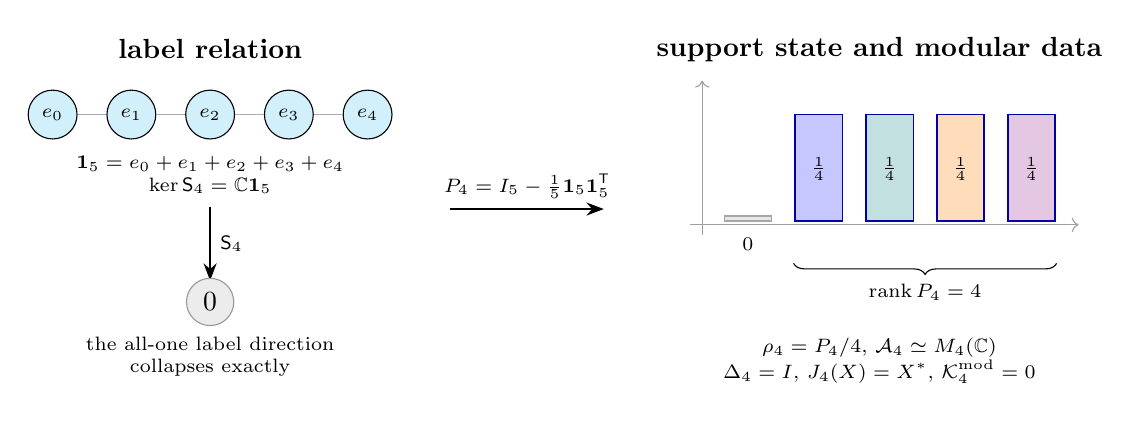
\begin{tikzpicture}[
  x=1cm,y=1cm,
  labelnode/.style={circle,draw=black,fill=cyan!18,minimum size=6.2mm,
                    inner sep=0pt,font=\scriptsize},
  supportbar/.style={draw=blue!65!black,fill=blue!22,line width=0.55pt},
  kernelbar/.style={draw=gray!70,fill=gray!18,line width=0.55pt},
  flow/.style={-{Stealth[length=2.2mm]},line width=0.75pt}
]
\begin{scope}[xshift=-4.8cm]
  \node[font=\bfseries] at (0,2.18) {label relation};
  \foreach \x/\k in {-2/0,-1/1,0/2,1/3,2/4}
    \node[labelnode] (e\k) at (\x,1.35) {\(e_{\k}\)};
  \draw[gray!65,line width=0.45pt]
    (e0)--(e1)--(e2)--(e3)--(e4);
  \node[font=\scriptsize,align=center] at (0,0.58)
    {\(\mathbf 1_5=e_0+e_1+e_2+e_3+e_4\)\\
     \(\ker\mathsf S_4=\mathbb C\mathbf 1_5\)};
  \draw[flow] (0,0.18)--(0,-0.76)
    node[midway,right,font=\scriptsize] {\(\mathsf S_4\)};
  \node[circle,draw=gray!80,fill=gray!15,minimum size=6mm,
        inner sep=0pt] at (0,-1.03) {\(0\)};
  \node[font=\scriptsize,align=center] at (0,-1.72)
    {the all-one label direction\\collapses exactly};
\end{scope}

\draw[flow] (-1.75,0.15)--(0.2,0.15)
  node[midway,above,font=\scriptsize]
  {\(P_4=I_5-\frac15\mathbf 1_5\mathbf 1_5^{\mathsf T}\)};

\begin{scope}[xshift=1.45cm]
  \node[font=\bfseries] at (2.25,2.18) {support state and modular data};
  \draw[->,gray!75] (-0.15,-0.05)--(4.78,-0.05);
  \draw[->,gray!75] (0,-0.18)--(0,1.78);
  \path[kernelbar] (0.28,0)--(0.88,0)--(0.88,0.06)--(0.28,0.06)--cycle;
  \foreach \x/\c in {1.18/blue!22,2.08/teal!24,2.98/orange!27,3.88/violet!22}
    \path[draw=blue!65!black,fill=\c,line width=0.55pt]
      (\x,0)--(\x+0.6,0)--(\x+0.6,1.35)--(\x,1.35)--cycle;
  \node[font=\scriptsize] at (0.58,-0.30) {\(0\)};
  \foreach \x in {1.48,2.38,3.28,4.18}
    \node[font=\scriptsize] at (\x,0.66) {\(\frac14\)};
  \draw[decorate,decoration={brace,mirror,amplitude=4pt}]
    (1.16,-0.54)--(4.50,-0.54)
    node[midway,below=4pt,font=\scriptsize]
    {\(\operatorname{rank}P_4=4\)};
  \node[font=\scriptsize,align=center] at (2.25,-1.78)
    {\(\rho_4=P_4/4\), \(\mathcal A_4\simeq M_4(\mathbb C)\)\\
     \(\Delta_4=I\), \(J_4(X)=X^\ast\),
     \(\mathcal K_4^{\mathrm{mod}}=0\)};
\end{scope}
\end{tikzpicture}
\caption{The exact support mechanism for the regular \(4\)-simplex.
The synthesis map kills precisely the all-one label line.  Projection onto
its orthogonal complement leaves a rank-four support carrying four equal
state eigenvalues \(1/4\).  On the resulting matrix corner the Tomita
operator is adjunction and the modular operator is the identity.}
\label{fig:regular-four-simplex-modular-support}
\end{figure}

\begin{computation}[Exact check of the simplex rank--volume identities]
\label{comp:regular-simplex-dimension-volume-check}
The script and captured receipt
\[
\begin{gathered}
 \texttt{verification/verify\_regular\_simplex\_dimension\_volume.py},\\
 \texttt{verification/verify\_regular\_simplex\_dimension\_volume\_output.txt}
\end{gathered}
\]
check the centered and projected spectra, ranks, pseudodeterminants,
edge-Gram determinants, both volume formulas, the altitude identity, the
two trace-one state spectra and purities, and both control-length formulas
for every \(2\leq n\leq12\).  They also check the exact \(n=4\) values in
\eqref{eq:regular-four-simplex-rank-volume-data}, the four eigenvalues
equal to \(1/4\) in \(\rho_4\), and the two lengths in
\eqref{eq:regular-four-simplex-control-length-volume}.
\end{computation}

\begin{figure}[htbp]
\centering
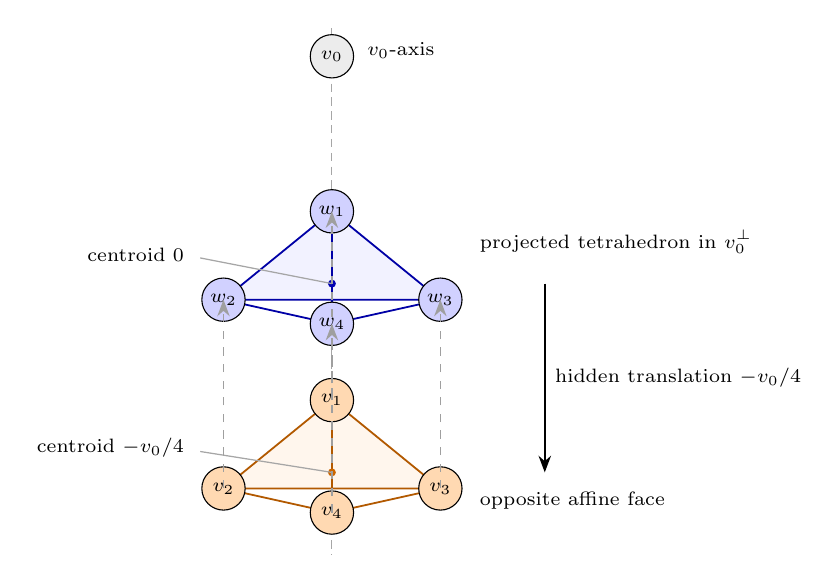
\begin{tikzpicture}[
  scale=1.02,
  vertex/.style={circle,draw=black,minimum size=5.5mm,inner sep=0pt,
                 font=\scriptsize},
  projected/.style={vertex,fill=blue!18},
  actual/.style={vertex,fill=orange!30},
  edgep/.style={draw=blue!65!black,line width=0.65pt},
  edgea/.style={draw=orange!70!black,line width=0.65pt},
  projection/.style={-{Stealth[length=2.1mm]},dashed,gray!75,line width=0.55pt}
]
\coordinate (A) at (0,3.65);
\coordinate (O) at (0,0.82);
\coordinate (C) at (0,-1.53);

\coordinate (W1) at (0,1.72);
\coordinate (W2) at (-1.35,0.62);
\coordinate (W3) at (1.35,0.62);
\coordinate (W4) at (0,0.32);

\coordinate (V1) at (0,-0.63);
\coordinate (V2) at (-1.35,-1.73);
\coordinate (V3) at (1.35,-1.73);
\coordinate (V4) at (0,-2.03);

\draw[dash pattern=on 3pt off 2pt,gray!70] (0,4.0)--(0,-2.55);
\node[vertex,fill=gray!15] at (A) {$v_0$};
\node[font=\scriptsize,anchor=west] at (0.32,3.72) {\(v_0\)-axis};

\fill[blue!5] (W1)--(W2)--(W3)--cycle;
\draw[edgep] (W1)--(W2)--(W3)--cycle;
\draw[edgep] (W4)--(W1);
\draw[edgep] (W4)--(W2);
\draw[edgep] (W4)--(W3);
\node[projected] at (W1) {\(w_1\)};
\node[projected] at (W2) {\(w_2\)};
\node[projected] at (W3) {\(w_3\)};
\node[projected] at (W4) {\(w_4\)};
\fill[blue!70!black] (O) circle (1.4pt);
\node[font=\scriptsize,anchor=west] at (1.72,1.34)
  {projected tetrahedron in \(v_0^\perp\)};
\node[font=\scriptsize,anchor=east] at (-1.72,1.18) {centroid \(0\)};
\draw[gray!70,line width=0.45pt] (-1.64,1.14)--(O);

\fill[orange!7] (V1)--(V2)--(V3)--cycle;
\draw[edgea] (V1)--(V2)--(V3)--cycle;
\draw[edgea] (V4)--(V1);
\draw[edgea] (V4)--(V2);
\draw[edgea] (V4)--(V3);
\node[actual] at (V1) {\(v_1\)};
\node[actual] at (V2) {\(v_2\)};
\node[actual] at (V3) {\(v_3\)};
\node[actual] at (V4) {\(v_4\)};
\fill[orange!80!black] (C) circle (1.4pt);
\node[font=\scriptsize,anchor=west] at (1.72,-1.88)
  {opposite affine face};
\node[font=\scriptsize,anchor=east] at (-1.72,-1.22)
  {centroid \(-v_0/4\)};
\draw[gray!70,line width=0.45pt] (-1.64,-1.27)--(C);

\draw[projection] (V1)--(W1);
\draw[projection] (V2)--(W2);
\draw[projection] (V3)--(W3);
\draw[projection] (V4)--(W4);
\draw[-{Stealth[length=2.1mm]},line width=0.75pt]
  (2.65,0.82)--(2.65,-1.53)
  node[midway,right,font=\scriptsize] {hidden translation \(-v_0/4\)};
\end{tikzpicture}
\caption{The \(n=4\) case of vertex projection.  The orange opposite face
is the blue projected tetrahedron translated by \(-v_0/4\).  Orthogonal
projection along the \(v_0\)-axis identifies corresponding vertices and
sends the orange centroid to \(0\).  The two tetrahedra are drawn in the
same oblique image of their internal three coordinates; their vertical
separation records the fourth coordinate.}
\label{fig:four-simplex-hidden-quarter-projection}
\end{figure}

\begin{computation}[Exact check of the simplex-projection identities]
\label{comp:regular-simplex-projection-check}
The script and captured receipt
\[
\begin{gathered}
 \texttt{verification/verify\_regular\_simplex\_projection.py},\\
 \texttt{verification/verify\_regular\_simplex\_projection\_output.txt}
\end{gathered}
\]
check the symbolic diagonal and off-diagonal formulas, the unit-rescaled
Gram entry, the complete Gram matrices for \(2\leq n\leq9\), and the exact
\(n=4\) entries \(15/16\), \(-5/16\), and \(-v_0/4\).
\end{computation}

\begin{theorem}[The Fable rays force a regular \(4\)-simplex completion]
\label{thm:Fable-forced-regular-four-simplex}
Let
\[
 U_+
 :=
 \operatorname{span}_{\mathbb R}\{E_{11},E_{12},E_{22}\},
\]
and retain the three Fable rays \(r_0,r_+,r_-\) from
\eqref{eq:Fable-null-rays-raw-cell-preimages}.  Define the fourth centered
ray
\begin{equation}
 r_\infty:=-(r_0+r_++r_-)
 =-6(E_{11}+E_{22}).
 \label{eq:Fable-forced-fourth-positive-ray}
\end{equation}
There is a unique symmetric bilinear form on \(U_+\) satisfying
\begin{equation}
 \langle r_a,r_b\rangle_{G_+}
 =
 \begin{cases}
 1,&a=b,\\[1mm]
 -\dfrac13,&a\ne b,
 \end{cases}
 \qquad
 a,b\in\{\infty,0,+,-\}.
 \label{eq:Fable-positive-tetrahedral-Gram}
\end{equation}
In the ordered basis \((E_{11},E_{12},E_{22})\), its matrix is
\begin{equation}
 G_+
 =
 \begin{pmatrix}
  \dfrac1{16}&0&-\dfrac7{144}\\[2mm]
  0&\dfrac29&0\\[2mm]
  -\dfrac7{144}&0&\dfrac1{16}
 \end{pmatrix},
 \qquad
 \operatorname{Spec}(G_+)
 =
 \left\{\frac1{72},\frac19,\frac29\right\}.
 \label{eq:Fable-forced-positive-metric}
\end{equation}
In particular, \(G_+\) is positive definite and the four rays in
\eqref{eq:Fable-positive-tetrahedral-Gram} are the vertices of a centered
regular tetrahedron.

Extend \(G_+\) to the full raw-cell space by requiring \(E_{21}\) to be
unit and orthogonal to \(U_+\).  In the ordered raw-cell basis this gives
\begin{equation}
 \widehat G_{\mathrm F}
 =
 \begin{pmatrix}
  \dfrac1{16}&0&0&-\dfrac7{144}\\[2mm]
  0&\dfrac29&0&0\\[2mm]
  0&0&1&0\\[2mm]
  -\dfrac7{144}&0&0&\dfrac1{16}
 \end{pmatrix}.
 \label{eq:Fable-forced-full-metric}
\end{equation}
For \(a\in\{\infty,0,+,-\}\), put
\begin{equation}
 s_\ast:=E_{21},
 \qquad
 s_a:=\frac{\sqrt{15}}4r_a-\frac14E_{21}.
 \label{eq:Fable-regular-four-simplex-vertices}
\end{equation}
Then
\begin{equation}
 \langle s_\alpha,s_\beta\rangle_{\widehat G_{\mathrm F}}
 =
 \begin{cases}
 1,&\alpha=\beta,\\[1mm]
 -\dfrac14,&\alpha\ne\beta,
 \end{cases}
 \qquad
 \alpha,\beta\in\{\ast,\infty,0,+,-\}.
 \label{eq:Fable-regular-four-simplex-Gram}
\end{equation}
Thus the five displayed vectors form a regular \(4\)-simplex.  Its face
opposite \(s_\ast\) has centroid
\begin{equation}
 \frac14(s_\infty+s_0+s_++s_-)
 =-\frac14E_{21},
 \label{eq:Fable-regular-four-simplex-centroid}
\end{equation}
and its orthogonal projection to \(U_+\) is the regular tetrahedron with
vertices \((\sqrt{15}/4)r_a\).

The operators \(\mathfrak R_\square\) and
\(\mathfrak J_\square\) preserve \(\widehat G_{\mathrm F}\), fix
\(s_\ast\) and \(s_\infty\), and act on \(s_0,s_+,s_-\) by the cycle and
reflection in
\eqref{eq:Fable-tetrahedron-C3-action}--%
\eqref{eq:Fable-tetrahedron-C2-action}.  Hence the maintained Fable
\(D_3\) action is an orthogonal vertex symmetry of the completed regular
\(4\)-simplex.

Finally, the centroid axis intertwines the regular-simplex quarter with the
maintained coefficient inversion:
\begin{equation}
 \mathcal T_\square\!\left(-\frac14E_{21}\right)
 =
 \mathcal I_-\mathcal T_\square(E_{21})
 =
 -\frac18(4,0,0,-1).
 \label{eq:Fable-simplex-axis-intertwiner}
\end{equation}
If \(\iota_1(t)=(t,0,0)\), then the common Fable output is
\begin{equation}
 F(p_0)=F(p_+)=F(p_-)
 =\iota_1\!\left(-\frac14\right).
 \label{eq:Fable-simplex-quarter-output}
\end{equation}
The same scalar \(-1/4\) therefore occurs as the opposite-face
displacement, the simple inversion eigenvalue, and the first coordinate of
the three-point Fable output.
\end{theorem}

\begin{proof}
In the ordered basis \((E_{11},E_{12},E_{22})\), let
\[
 P_+
 :=
 \begin{pmatrix}
  2&2+\sqrt3&2-\sqrt3\\
  2&-1&-1\\
  2&2-\sqrt3&2+\sqrt3
 \end{pmatrix},
 \qquad
 H_3
 :=
 \begin{pmatrix}
  1&-\frac13&-\frac13\\
  -\frac13&1&-\frac13\\
  -\frac13&-\frac13&1
 \end{pmatrix}.
\]
The columns of \(P_+\) are \(r_0,r_+,r_-\), and
\(\det P_+=-24\sqrt3\).  A symmetric form with Gram matrix \(H_3\) on
these three basis vectors must therefore have matrix
\[
 (P_+^{-1})^{\mathsf T}H_3P_+^{-1}.
\]
Exact multiplication gives the matrix \(G_+\) in
\eqref{eq:Fable-forced-positive-metric}.  Its three eigenvalues are
positive.  Since \(r_\infty=-(r_0+r_++r_-)\), multiplication by the
complete \(4\times4\) Gram matrix gives
\eqref{eq:Fable-positive-tetrahedral-Gram}.  This also proves uniqueness.

The extension conditions determine
\(\widehat G_{\mathrm F}\) uniquely and give
\eqref{eq:Fable-forced-full-metric}.  Substituting
\eqref{eq:Fable-positive-tetrahedral-Gram} into
\eqref{eq:Fable-regular-four-simplex-vertices} gives
\[
 \langle s_a,s_a\rangle
 =\frac{15}{16}+\frac1{16}=1,
 \qquad
 \langle s_a,s_b\rangle
 =-\frac5{16}+\frac1{16}=-\frac14
 \quad(a\ne b),
\]
and
\[
 \langle s_\ast,s_a\rangle=-\frac14.
\]
This proves \eqref{eq:Fable-regular-four-simplex-Gram}.  Summing the four
opposite vertices and using
\(\sum_ar_a=0\) proves
\eqref{eq:Fable-regular-four-simplex-centroid}.

The exact ray action in
\eqref{eq:Fable-D3-raw-null-ray-action} permutes
\(r_0,r_+,r_-\) and therefore fixes their negative sum \(r_\infty\).
It preserves every entry of
\eqref{eq:Fable-positive-tetrahedral-Gram}; hence it preserves \(G_+\).
Both generators fix \(E_{21}\), proving preservation of
\(\widehat G_{\mathrm F}\) and the stated vertex action.

Equation \eqref{eq:four-cell-explicit-quarter-images} gives
\[
 \mathcal T_\square(E_{21})
 =\frac12(4,0,0,-1),
\]
and \eqref{eq:target-cell-negative-quarter} gives its
\(-1/4\) eigenvalue.  Linearity proves
\eqref{eq:Fable-simplex-axis-intertwiner}.  Equation
\eqref{eq:Fable-simplex-quarter-output} is the exact common-fibre
evaluation in \cref{thm:complete-fable-fibre}.
\end{proof}

\begin{figure}[htbp]
\centering
\includegraphics[width=0.76\linewidth]
{figures/fable_regular_tetrahedron.pdf}
\caption{A three-dimensional isometric realization of the exact ray Gram
form \eqref{eq:Fable-positive-tetrahedral-Gram}.  The plotted coordinates
are \(r_\infty=(1,1,1)/\sqrt3\),
\(r_0=(1,-1,-1)/\sqrt3\),
\(r_+=(-1,1,-1)/\sqrt3\), and
\(r_-=(-1,-1,1)/\sqrt3\).
Every distinct pair has inner product \(-1/3\).  The blue arrows realize
the \(C_3\) action on the opposite face; its dashed gray axis realizes the
reflection fixing \(r_0\) and exchanging \(r_+\) with \(r_-\).  The red
dashed altitude ends at the exact face centroid
\(c_{\mathrm{face}}=-r_\infty/3\).}
\label{fig:Fable-exact-regular-tetrahedron}
\end{figure}

\begin{computation}[Exact check of the regular-tetrahedron vector image]
\label{comp:Fable-regular-tetrahedron-image-check}
The generator, checker, and captured receipt
\[
\begin{gathered}
 \texttt{verification/make\_fable\_regular\_tetrahedron.py},\\
 \texttt{verification/verify\_fable\_regular\_tetrahedron\_figure.py},\\
 \texttt{verification/verify\_fable\_regular\_tetrahedron\_figure\_output.txt}
\end{gathered}
\]
verify the complete Gram matrix, zero centroid, opposite-face centroid,
altitude, three face-edge lengths, and reflection axis used in
\cref{fig:Fable-exact-regular-tetrahedron}.  The maintained image is the
vector PDF
\(\texttt{figures/fable\_regular\_tetrahedron.pdf}\).
\end{computation}

\begin{computation}[Exact verification of the Fable \(4\)-simplex completion]
\label{comp:Fable-regular-four-simplex-check}
The checker and captured receipt
\[
\begin{gathered}
 \texttt{verification/verify\_fable\_regular\_four\_simplex.py},\\
 \texttt{verification/verify\_fable\_regular\_four\_simplex\_output.txt}
\end{gathered}
\]
verify the forced fourth vertex, the positive spectrum of \(G_+\), the
regular-tetrahedron and regular-\(4\)-simplex Gram matrices, exact
\(D_3\)-invariance and vertex actions, the face centroid, the axis
intertwiner, and all three polynomial evaluations in
\eqref{eq:Fable-simplex-quarter-output}.
\end{computation}

\begin{corollary}[The exact \(109\to53\to\) quarter-circle transport chain]
\label{cor:109-53-quarter-circle-chain}
The single matrix \(P_\square\) satisfies
\begin{equation}
 2\,\mathscr H_\square(\mathcal M(109))
 \xmapsto{\ \mathscr A_{P_\square}\ }
 \mathscr H_\square(\mathcal M(53))
 \xmapsto{\ \mathscr A_{P_\square}\ }
 \begin{pmatrix}4&0\\0&-1\end{pmatrix}.
 \label{eq:109-53-quarter-Hermitian-chain}
\end{equation}
Explicitly,
\begin{equation}
 2H(0,1,0,0)
 \xmapsto{\ \mathscr A_{P_\square}\ }
 H(0,0,2,0)
 \xmapsto{\ \mathscr A_{P_\square}\ }
 H(4,0,0,-1).
 \label{eq:109-53-quarter-coefficient-chain}
\end{equation}
In generalized-circle equations, the same chain is
\begin{equation}
 4x=0
 \quad\longmapsto\quad
 -4y=0
 \quad\longmapsto\quad
 4(x^2+y^2)-1=0.
 \label{eq:109-53-quarter-circle-chain}
\end{equation}
The coefficient two in the first term is required:
\(\mathcal M(109)=E_{12}\), whereas
\(\mathcal M(53)=2E_{21}\).
\end{corollary}

\begin{proof}
The first two basis images in
\eqref{eq:four-cell-explicit-quarter-images} give
\[
 \mathscr A_{P_\square}
 \bigl(H(0,1,0,0)\bigr)
 =H(0,0,1,0).
\]
Linearity gives
\[
 \mathscr A_{P_\square}
 \bigl(2H(0,1,0,0)\bigr)
 =H(0,0,2,0)
 =\mathscr H_\square(\mathcal M(53)).
\]
Equation \eqref{eq:blade-target-explicit-SL2-congruence} gives the second
arrow.  Finally, the generalized-circle evaluation
\[
 q_{(a,b_0,b_1,c)}(x,y)
 =a(x^2+y^2)+2b_0x-2b_1y+c
\]
gives the three displayed equations.
\end{proof}

\begin{theorem}[Multiplicity two identifies the quotient branch with the target carrier]
\label{thm:multiplicity-two-quarter-carrier}
For \(m>0\), let
\[
 N_m=mE_{21},
 \qquad
 P_{\mathrm s}(m)=N_m^{\mathsf T}N_m=m^2E_{11},
 \qquad
 Q_{\mathrm r}=E_{22}.
\]
For each \(\zeta\in\mathbb R\), there is a unique diagonal coefficient matrix
\(\jmath_m(\zeta)\) satisfying
\begin{equation}
 \jmath_m(\zeta)-P_{\mathrm s}(m)\in\mathbb RQ_{\mathrm r},
 \qquad
 \frac{C(\jmath_m(\zeta))}{A(\jmath_m(\zeta))}=\zeta.
 \label{eq:quotient-section-characterization}
\end{equation}
It is
\begin{equation}
 \jmath_m(\zeta)
 =P_{\mathrm s}(m)+m^2\zeta Q_{\mathrm r}
 =\begin{pmatrix}m^2&0\\0&m^2\zeta\end{pmatrix}.
 \label{eq:quotient-to-blade-section}
\end{equation}
For \(\zeta<0\), the coefficient inversion associated with
\(\jmath_m(\zeta)\) is nondegenerate and has simple normal eigenvalue
\begin{equation}
 -\frac{\Norm(\jmath_m(\zeta))}{A(\jmath_m(\zeta))^2}
 =\frac{C(\jmath_m(\zeta))}{A(\jmath_m(\zeta))}
 =\zeta.
 \label{eq:quotient-section-normal-eigenvalue}
\end{equation}
Its Sarnak coordinates in the \(X=Y=0\) plane are
\begin{equation}
 T_m(\zeta)=\frac{m^2}{2}(1+\zeta),
 \qquad
 W_m(\zeta)=\frac{m^2}{2}(1-\zeta).
 \label{eq:quotient-section-TW}
\end{equation}

At the denominator-exchange branch value
\(\zeta_{\mathrm{br}}=-1/4\) of
\cref{thm:ES-quarter-branch},
\begin{equation}
 \jmath_m(\zeta_{\mathrm{br}})
 =m^2E_{11}-\frac{m^2}{4}E_{22}.
 \label{eq:branch-section-general-m}
\end{equation}
The equality
\begin{equation}
 \jmath_m(\zeta_{\mathrm{br}})
 =P_{\mathrm s}(m)-Q_{\mathrm r}
 \label{eq:branch-equals-idempotent-support}
\end{equation}
holds exactly for \(m=2\).  Therefore the positive transport multiplicity
two is uniquely characterized by the requirement that the universal branch
value supply the negative occupied target idempotent.  For the observed
blade coefficient \(N=N_2\),
\begin{equation}
 \jmath_2\left(-\frac14\right)
 =4E_{11}-E_{22}
 =\mathfrak H(N),
 \label{eq:observed-branch-carrier-identity}
\end{equation}
and \eqref{eq:quotient-section-TW} gives
\((T,W)=(3/2,5/2)\).
\end{theorem}

\begin{proof}
Any matrix in the affine line specified by the first condition of
\eqref{eq:quotient-section-characterization} has the form
\[
 K=P_{\mathrm s}(m)+cQ_{\mathrm r}
  =\operatorname{diag}(m^2,c).
\]
Its coefficient ratio is \(C(K)/A(K)=c/m^2\).  The second condition therefore
forces \(c=m^2\zeta\), proving existence, uniqueness, and
\eqref{eq:quotient-to-blade-section}.

For \(\zeta<0\),
\[
 \Norm(\jmath_m(\zeta))
 =-m^4\zeta>0.
\]
The reflection factorization
\[
 M_w=\frac{\Norm(w)}{A(w)^2}R_w
\]
shows that the eigenvalue on the normal line is
\[
 -\frac{-m^4\zeta}{m^4}=\zeta,
\]
which proves \eqref{eq:quotient-section-normal-eigenvalue}.  Substitution of
\(A=m^2\) and \(C=m^2\zeta\) into
\(T=(A+C)/2\) and \(W=(A-C)/2\) proves
\eqref{eq:quotient-section-TW}.

At \(\zeta=-1/4\), equation
\eqref{eq:quotient-to-blade-section} gives
\eqref{eq:branch-section-general-m}.  Comparing its \(E_{22}\)-coefficient
with that of \(P_{\mathrm s}(m)-Q_{\mathrm r}\) gives
\[
 \frac{m^2}{4}=1.
\]
Since \(m>0\), this is equivalent to \(m=2\).  The final identities follow
by substitution.
\end{proof}

\begin{theorem}[Kocik parameter and Fable-slice coordinates of the target
carrier]
\label{thm:target-carrier-Kocik-Fable-slice}
Let \(m>0\) and \(-1/4\le\zeta<0\).  The Sarnak coordinates of
\(\jmath_m(\zeta)\) are
\[
 (T,X,Y,W)
 =\left(
   \frac{m^2}{2}(1+\zeta),\,0,\,0,\,
   \frac{m^2}{2}(1-\zeta)
  \right).
\]
Define
\begin{equation}
 p(\zeta)
 :=\frac{1+\zeta^2}{1-4\zeta+\zeta^2}.
 \label{eq:target-carrier-Kocik-parameter}
\end{equation}
Then
\begin{equation}
 \frac{X^2+Y^2+W^2}{T^2}
 =\left(\frac{1-\zeta}{1+\zeta}\right)^2
 =\frac{p(\zeta)+1}{3p(\zeta)-1}.
 \label{eq:target-carrier-Kocik-cone}
\end{equation}
Thus \(\jmath_m(\zeta)\) lies on the member with configuration parameter
\(p(\zeta)\) of Kocik's equal-angle quadratic family
\eqref{eq:Kocik-Sarnak-cone}.  Along the full carrier segment,
\[
 p\!\left(-\frac14\right)=\frac{17}{33},
 \qquad
 p(-4+\sqrt{15})=\frac23,
 \qquad
 \lim_{\zeta\to0^-}p(\zeta)=1.
\]
The function \(p(\zeta)\) is strictly increasing on
\([-1/4,0)\).

For the champion coordinate
\[
 \zeta_\ast=-\frac{18189}{18190^2},
\]
the exact Kocik parameter is
\begin{equation}
 p_\ast
 =\frac{109478993882049721}{109503067103581321}.
 \label{eq:champion-Kocik-parameter}
\end{equation}

The Lorentz isometry
\begin{equation}
 L_{XW}(T,X,Y,W)=(T,W,-Y,X)
 \label{eq:XW-SO-rotation}
\end{equation}
belongs to \(\mathrm{SO}^{+}(3,1)\) and sends the carrier point to the
\(W=0\) Fable slice.  More precisely,
\begin{equation}
 L_{XW}\Psi_{\mathrm{circ}}\bigl(\jmath_m(\zeta)\bigr)
 =\iota\left(
  \frac{m^2}{2}(1+\zeta),\,
  \frac{m^2}{\sqrt3}(1-\zeta),\,0
 \right),
 \label{eq:target-carrier-Fable-slice-coordinate}
\end{equation}
and the Fable quadratic form has the exact value
\begin{equation}
 q\left(
  \frac{m^2}{2}(1+\zeta),\,
  \frac{m^2}{\sqrt3}(1-\zeta),\,0
 \right)
 =m^4\zeta.
 \label{eq:target-carrier-Fable-slice-norm}
\end{equation}
The endpoint \(\zeta=0\) is the Descartes--Fable null cone.  Relative to the
displayed Lorentz form \(T^2-X^2-Y^2-W^2\), every point with
\(\zeta<0\) is spacelike.
\end{theorem}

\begin{proof}
The coordinate formula is \eqref{eq:quotient-section-TW}.  Since
\(X=Y=0\),
\[
 \frac{X^2+Y^2+W^2}{T^2}
 =\frac{(1-\zeta)^2}{(1+\zeta)^2}.
\]
Solving
\[
 \frac{(1-\zeta)^2}{(1+\zeta)^2}
 =\frac{p+1}{3p-1}
\]
for \(p\) gives \eqref{eq:target-carrier-Kocik-parameter}, proving
\eqref{eq:target-carrier-Kocik-cone}.  Direct substitution gives
\[
 p(-1/4)=17/33,\qquad p(0)=1.
\]
The equation \(p(\zeta)=2/3\) is
\[
 \zeta^2+8\zeta+1=0.
\]
Its root in \([-1/4,0)\) is \(-4+\sqrt{15}\).  Differentiation gives
\[
 p'(\zeta)
 =\frac{4(1-\zeta^2)}
        {(1-4\zeta+\zeta^2)^2}>0
\]
throughout the stated interval.

For \(\zeta_\ast=-n/(n+1)^2\) with \(n=18189\),
\[
 p(\zeta_\ast)
 =\frac{(n+1)^4+n^2}
        {(n+1)^4+4n(n+1)^2+n^2}.
\]
Exact integer evaluation gives
\eqref{eq:champion-Kocik-parameter}; its numerator and denominator are
coprime.

The spatial part of \(L_{XW}\) exchanges the \(X\)- and \(W\)-axes and
changes the sign of the \(Y\)-axis.  Its determinant is \(1\), it fixes \(T\),
and it preserves \(X^2+Y^2+W^2-T^2\), proving the group assertion.
The definition of \(\iota\) in
\eqref{eq:Fable-Descartes-embedding} then gives
\eqref{eq:target-carrier-Fable-slice-coordinate}.  Finally,
\begin{align*}
 q&\left(
  \frac{m^2}{2}(1+\zeta),\,
  \frac{m^2}{\sqrt3}(1-\zeta),\,0
 \right)\\
 &=\frac{m^4}{4}(1+\zeta)^2
   -\frac{m^4}{4}(1-\zeta)^2
 =m^4\zeta,
\end{align*}
which proves \eqref{eq:target-carrier-Fable-slice-norm}.
\end{proof}

\begin{proposition}[The arithmetic cubic family and its Lorentz
discriminant]
\label{prop:arithmetic-cubic-Lorentz-discriminant}
For \(\zeta\in\mathbb R\), define
\[
 C_\zeta(U,V):=U^2V+\zeta V^3.
\]
For \(\mathbf u=(U,V)^{\mathsf T}\),
\begin{equation}
 m^2C_\zeta(U,V)
 =V\,\mathbf u^{\mathsf T}\jmath_m(\zeta)\mathbf u.
 \label{eq:arithmetic-cubic-carrier-restriction}
\end{equation}
Its binary-cubic discriminant is
\begin{equation}
 \operatorname{Disc}(C_\zeta)=-4\zeta,
 \label{eq:arithmetic-cubic-discriminant}
\end{equation}
and
\begin{equation}
 \Norm(\jmath_m(\zeta))
 =\frac{m^4}{4}\operatorname{Disc}(C_\zeta).
 \label{eq:arithmetic-cubic-Lorentz-discriminant}
\end{equation}
For \(m=2\),
\[
 \Norm(\jmath_2(\zeta))
 =4\operatorname{Disc}(C_\zeta),
 \qquad
 F_{\mathrm D}\bigl(\Psi_{\mathrm{circ}}(\jmath_2(\zeta))\bigr)
 =8\operatorname{Disc}(C_\zeta).
\]
At \(\zeta=-1/4\),
\[
 C_\zeta=C,\qquad
 \operatorname{Disc}(C)=1.
\]
Thus the common Fable cubic is the discriminant-one endpoint of the
arithmetic carrier family.
\end{proposition}

\begin{proof}
Equation \eqref{eq:quotient-to-blade-section} gives
\[
 \mathbf u^{\mathsf T}\jmath_m(\zeta)\mathbf u
 =m^2U^2+m^2\zeta V^2.
\]
Multiplication by \(V\) proves
\eqref{eq:arithmetic-cubic-carrier-restriction}.  For a binary cubic
\[
 aU^3+bU^2V+cUV^2+dV^3,
\]
the discriminant is
\[
 b^2c^2-4ac^3-4b^3d-27a^2d^2+18abcd.
\]
Substitution of
\[
 (a,b,c,d)=(0,1,0,\zeta)
\]
gives \eqref{eq:arithmetic-cubic-discriminant}.  Since
\[
 \Norm(\jmath_m(\zeta))=-m^4\zeta,
\]
equation \eqref{eq:arithmetic-cubic-Lorentz-discriminant} follows.
The Descartes relation is
\eqref{eq:circle-Sarnak-isometry}.  Substitution of
\(\zeta=-1/4\) proves the final statements.
\end{proof}

\begin{theorem}[Complete Fable fibre over the target-carrier line]
\label{thm:complete-Fable-carrier-line-fibre}
Let \(r\in\mathbb C^\times\).  Define
\begin{align}
 p_0(r)&=(0,0,-r^2),\notag\\
 p_+(r)&=\left(\frac1{2r},-3r,26r^2\right),\notag\\
 p_-(r)&=\left(-\frac1{2r},3r,26r^2\right).
 \label{eq:Fable-carrier-line-three-points}
\end{align}
Then
\begin{equation}
 F(p_0(r))=F(p_+(r))=F(p_-(r))=(-r^2,0,0).
 \label{eq:Fable-carrier-line-common-image}
\end{equation}
These are the complete three points of the fibre.  Each point is reduced.

The common invariant cubic is
\begin{equation}
 C_{-r^2}(U,V)
 =U^2V-r^2V^3
 =V(U-rV)(U+rV),
 \label{eq:Fable-carrier-line-cubic}
\end{equation}
and the three resultant-one marked factorizations supplied by the invariant
lift are
\begin{align}
 L_0&=V,
 &Q_0&=U^2-r^2V^2,\notag\\
 L_+&=\frac{U-rV}{2r},
 &Q_+&=2rV(U+rV),\notag\\
 L_-&=-\frac{U+rV}{2r},
 &Q_-&=-2rV(U-rV).
 \label{eq:Fable-carrier-line-factorizations}
\end{align}
\end{theorem}

\begin{proof}
For \(p_+(r)\), one has
\[
 xy=-\frac32,\qquad 1+xy=-\frac12,\qquad 4+3xy=-\frac12.
\]
Substitution in the three displayed coordinates of \(F\) gives
\begin{align*}
 F_1(p_+(r))
 &=-\frac18(26r^2)
   +9r^2\left(-\frac12\right)\left(-\frac12\right)
 =-r^2,\\
 F_2(p_+(r))
 &=-3r+\frac{39}{4}r-\frac{27}{4}r=0,\\
 F_3(p_+(r))
 &=\frac1r+\frac9{4r}-\frac{13}{4r}=0.
\end{align*}
The involution \(\sigma(x,y,z)=(-x,-y,z)\) sends \(p_+(r)\) to
\(p_-(r)\) and changes only the signs of \(F_2,F_3\), so
\eqref{eq:Fable-carrier-line-common-image} follows for \(p_-(r)\).
Substitution of \(p_0(r)\) is immediate.

The products in \eqref{eq:Fable-carrier-line-factorizations} are all
\eqref{eq:Fable-carrier-line-cubic}.  Under the resultant definition
\eqref{eq:linear-quadratic-resultant-definition}, their resultants are all
one.  Conversely, the resultant-one invariant lift of any point in the fibre
gives a resultant-one factorization of
\(C_{-r^2}\).  Since \(r\ne0\), this cubic has exactly the three distinct
projective linear factors
\[
 V,\qquad U-rV,\qquad U+rV.
\]
Choosing the marked linear factor determines its quadratic complement up to
reciprocal rescaling.  Under
\[
 (L,Q)\longmapsto(\lambda L,\lambda^{-1}Q),
\]
the linear--quadratic resultant is multiplied by \(\lambda\).  Hence the
resultant-one requirement fixes the rescaling uniquely, giving exactly
\eqref{eq:Fable-carrier-line-factorizations}.

The source coordinates are recovered from the lift coefficients by
\[
 x=a,\qquad 1+xy=b.
\]
When \(a\ne0\),
\[
 y=\frac{b-1}{a},
 \qquad
 z=\frac{2(1-\frac32xy-c)}{x^2}.
\]
These formulas recover \(p_+(r)\) and \(p_-(r)\) from the second and third
factorizations.  In the first factorization, \(a=0,b=c=1,d=0,e=-r^2\);
the lift formulas give \(x=0,y=2d=0,z=e=-r^2\).  Thus the three listed
points are the complete fibre.  Since \(\det JF=-2\), the Jacobian criterion
makes every point reduced.
\end{proof}

\begin{corollary}[Arithmetic divisor orbits as explicit Fable fibres]
\label{cor:arithmetic-orbit-explicit-Fable-fibre}
For positive \(N,d\), put
\begin{equation}
 r_d:=\frac{\sqrt{Nd}}{N+d}.
 \label{eq:arithmetic-Fable-radius}
\end{equation}
Then
\[
 \zeta_d=-r_d^2,
\]
and the divisor-complement involution satisfies
\begin{equation}
 r_{N^2/d}=r_d.
 \label{eq:arithmetic-Fable-radius-complement}
\end{equation}
Consequently every arithmetic carrier point
\(\mathcal J_{p,a}(d)\) determines the complete Fable fibre
\[
 \{p_0(r_d),p_+(r_d),p_-(r_d)\}
\]
over the target
\[
 (\zeta_d,0,0).
\]
The branch value \(d=N\) gives \(r_d=1/2\) and recovers the rational fibre
in \cref{thm:complete-fable-fibre}.
\end{corollary}

\begin{proof}
The first identity is the definition
\[
 \zeta_d=-\frac{Nd}{(N+d)^2}.
\]
Direct calculation gives
\[
 r_{N^2/d}
 =\frac{\sqrt{N^3/d}}{N+N^2/d}
 =\frac{\sqrt{Nd}}{N+d}
 =r_d.
\]
Apply \cref{thm:complete-Fable-carrier-line-fibre} with \(r=r_d\).
\end{proof}

\begin{theorem}[The Fable coordinate is the half-rapidity of the
Erd\H{o}s--Straus null vector]
\label{thm:Fable-half-rapidity}
Let \(d>0\), \(e=N^2/d\), and use the Sarnak coordinates
\[
 T=\frac{d+e}{2},\qquad X=N,\qquad Y=0,\qquad W=\frac{d-e}{2}.
\]
Put
\begin{equation}
 s=\frac12\log\frac dN,
 \qquad
 x_d=\frac{N+d}{2\sqrt{Nd}}.
 \label{eq:ES-rapidity-Fable-coordinate}
\end{equation}
Then
\begin{align}
 \frac TN&=\cosh(2s)=2x_d^2-1,\notag\\
 \frac WN&=\sinh(2s),\notag\\
 x_d&=\cosh s,\notag\\
 r_d&=\frac1{2x_d},\qquad
 \zeta_d=-\frac1{4x_d^2}.
 \label{eq:ES-Fable-half-rapidity-identities}
\end{align}
The two finite points of the corresponding Fable fibre can therefore be
written
\begin{equation}
 \left(x_d,-\frac{3}{2x_d},\frac{13}{2x_d^2}\right),
 \qquad
 \left(-x_d,\frac{3}{2x_d},\frac{13}{2x_d^2}\right).
 \label{eq:ES-Fable-half-rapidity-points}
\end{equation}
Moreover,
\begin{equation}
 \frac{W}{T+X}=\frac{d-N}{d+N}=\tanh s.
 \label{eq:ES-Fable-half-rapidity-asymmetry}
\end{equation}

The divisor-complement involution \(d\leftrightarrow e\) sends
\[
 s\longmapsto-s,\qquad W\longmapsto-W,
\]
and fixes \(x_d,r_d,\zeta_d\) and the three-point Fable fibre as a set.  The
Fable involution \(\sigma(x,y,z)=(-x,-y,z)\) exchanges the two points in
\eqref{eq:ES-Fable-half-rapidity-points} while fixing the arithmetic
orientation \(W\).  These are two distinct involutions.
\end{theorem}

\begin{proof}
Writing \(d/N=e^{2s}\) gives \(e/N=e^{-2s}\), so
\[
 \frac TN=\frac{e^{2s}+e^{-2s}}2=\cosh(2s),
 \qquad
 \frac WN=\frac{e^{2s}-e^{-2s}}2=\sinh(2s).
\]
Also
\[
 x_d
 =\frac{1+d/N}{2\sqrt{d/N}}
 =\frac{e^s+e^{-s}}2
 =\cosh s.
\]
The double-angle identity gives \(T/N=2x_d^2-1\).
Equation \eqref{eq:arithmetic-Fable-radius} gives
\[
 r_d=\frac{\sqrt{d/N}}{1+d/N}
     =\frac1{e^s+e^{-s}}
     =\frac1{2x_d},
\]
and hence \(\zeta_d=-r_d^2=-1/(4x_d^2)\).  Substitution in
\eqref{eq:Fable-carrier-line-three-points} proves
\eqref{eq:ES-Fable-half-rapidity-points}.

Finally,
\[
 \frac{W}{T+X}
 =\frac{d-e}{d+e+2N}
 =\frac{d-N}{d+N}
 =\frac{e^s-e^{-s}}{e^s+e^{-s}}
 =\tanh s.
\]
The two stated involution actions follow directly from these formulas and
from \(\sigma\).
\end{proof}

\begin{proposition}[Blade parity equals the Fable splitting squareclass]
\label{prop:blade-parity-Fable-squareclass}
Let
\[
 N=\prod_{i=1}^kq_i^{\alpha_i},
 \qquad
 d=\prod_{i=1}^kq_i^{\delta_i}\mid N^2,
 \qquad
 \beta_i=\delta_i-\alpha_i,
\]
where the \(q_i\) are distinct primes.  Put
\[
 \pi(\beta)=\{i:\beta_i\equiv1\pmod2\},
 \qquad
 s_\beta=\prod_{i\in\pi(\beta)}q_i.
\]
Then
\begin{equation}
 [Nd]=[s_\beta]
 \quad\text{in}\quad
 \mathbb Q^\times/(\mathbb Q^\times)^2.
 \label{eq:general-blade-Fable-squareclass}
\end{equation}
Consequently
\begin{equation}
 \mathbb Q(r_d)=\mathbb Q(\sqrt{s_\beta}),
 \label{eq:general-blade-Fable-splitting-field}
\end{equation}
with the understanding that the field is \(\mathbb Q\) when
\(s_\beta=1\).  Complementation sends \(\beta\) to \(-\beta\) and preserves
\(\pi(\beta)\), \(s_\beta\), and the splitting field.
\end{proposition}

\begin{proof}
For every \(i\),
\[
 \alpha_i+\delta_i
 \equiv\delta_i-\alpha_i
 =\beta_i\pmod2.
\]
Removing even exponents from
\[
 Nd=\prod_iq_i^{\alpha_i+\delta_i}
\]
gives \eqref{eq:general-blade-Fable-squareclass}.  Since
\[
 r_d=\frac{\sqrt{Nd}}{N+d}
\]
and the denominator is rational,
\eqref{eq:general-blade-Fable-splitting-field} follows.  If
\(d'=N^2/d\), then its centered exponent vector is
\[
 (2\alpha_i-\delta_i)-\alpha_i=-\beta_i.
\]
Parity is unchanged under negation.
\end{proof}

\begin{theorem}[The shell congruence is a square root of minus one in the
blade field]
\label{thm:shell-root-minus-one-blade-field}
Use the notation of
\cref{prop:blade-parity-Fable-squareclass}.  Let
\[
 \eta_i\in\{0,1\},\qquad
 \eta_i\equiv\beta_i\pmod2,
 \qquad
 \gamma_i=\frac{\beta_i-\eta_i}{2},
\]
and put
\[
 t_\beta=\prod_iq_i^{\gamma_i},
 \qquad
 \nu_\beta=t_\beta\sqrt{s_\beta}.
\]
Then
\begin{equation}
 \frac dN=t_\beta^2s_\beta=\nu_\beta^2.
 \label{eq:blade-field-half-eigenvalue}
\end{equation}

Assume that \(R\) is an odd prime, \(\gcd(R,N)=1\), and
\[
 d\equiv-N\pmod R.
\]
For every prime \(\mathfrak R\) of
\(\mathbb Q(\sqrt{s_\beta})\) above \(R\),
\begin{equation}
 \overline{\nu}_\beta^{\,2}=-1
 \quad\text{in the residue field at }\mathfrak R.
 \label{eq:residual-root-minus-one}
\end{equation}
Consequently
\begin{equation}
 \left(\frac{s_\beta}{R}\right)
 =\left(\frac{-1}{R}\right).
 \label{eq:blade-Legendre-condition}
\end{equation}

If \(R\equiv3\pmod4\), then \(s_\beta\) is a quadratic nonresidue modulo
\(R\), the prime \(R\) is inert in
\(\mathbb Q(\sqrt{s_\beta})\), and the residue field is
\(\mathbb F_{R^2}\).  In that field,
\begin{equation}
 \overline{\nu}_\beta^{\,R}
 =-\overline{\nu}_\beta
 =\overline{\nu}_\beta^{-1}.
 \label{eq:Frobenius-complement-root}
\end{equation}
The divisor-complement eigenvalue is \(\nu_\beta^{-1}\), so its reduction is
the Frobenius conjugate of \(\overline{\nu}_\beta\).
\end{theorem}

\begin{proof}
Since \(\beta_i=2\gamma_i+\eta_i\),
\[
 \frac dN=\prod_iq_i^{\beta_i}
 =\left(\prod_iq_i^{\gamma_i}\right)^2
  \prod_iq_i^{\eta_i}
 =t_\beta^2s_\beta,
\]
which proves \eqref{eq:blade-field-half-eigenvalue}.  Reduction of
\(d/N\equiv-1\pmod R\) proves
\eqref{eq:residual-root-minus-one}.  Because \(t_\beta\) is a nonzero square
modulo \(R\), Euler's criterion gives
\eqref{eq:blade-Legendre-condition}.

For \(R\equiv3\pmod4\), the right side of
\eqref{eq:blade-Legendre-condition} is \(-1\).  Hence the quadratic
polynomial defining the blade field is irreducible modulo \(R\), so the
residue degree is two.  The element
\(\overline{\nu}_\beta\) is a root of \(X^2+1\) outside \(\mathbb F_R\).
Frobenius permutes the two roots and therefore sends it to
\(-\overline{\nu}_\beta\).  Equation
\(\overline{\nu}_\beta^2=-1\) also gives
\(\overline{\nu}_\beta^{-1}=-\overline{\nu}_\beta\), proving
\eqref{eq:Frobenius-complement-root}.  Complementation replaces
\(d/N\) by \(N/d\) and hence replaces the half-eigenvalue by its inverse.
\end{proof}

\begin{theorem}[The arithmetic half-boost specializes to the Fable
inversion matrix on the shell]
\label{thm:arithmetic-half-boost-Fable-inversion}
Let \(N,d>0\), put \(e=N^2/d\), and choose the positive square root
\(\rho_d=\sqrt{Nd}\).  Define
\begin{equation}
 S_d:=\frac1{2\rho_d}
 \begin{pmatrix}
  N+d&d-N\\
  d-N&N+d
 \end{pmatrix},
 \qquad
 B_d:=\frac1N
 \begin{pmatrix}
  T&W\\
  W&T
 \end{pmatrix},
 \label{eq:arithmetic-half-boost-matrices}
\end{equation}
where
\[
 T=\frac{d+e}{2},
 \qquad
 W=\frac{d-e}{2}.
\]
Then
\begin{equation}
 \det S_d=1,
 \qquad
 S_d^2=B_d.
 \label{eq:arithmetic-half-boost-square}
\end{equation}
The vectors \((1,1)^{\mathsf T}\) and \((1,-1)^{\mathsf T}\) are
eigenvectors of \(S_d\), with the ordered eigenvalues
\begin{equation}
 \nu_d:=\frac{\rho_d}{N}=\sqrt{\frac dN},
 \qquad
 \nu_d^{-1}=\frac{\rho_d}{d}=\sqrt{\frac Nd}.
 \label{eq:arithmetic-half-boost-eigenvalues}
\end{equation}
With the compatible positive square root for \(e\), divisor
complementation satisfies
\begin{equation}
 S_e=S_d^{-1}.
 \label{eq:arithmetic-half-boost-complement}
\end{equation}

Put \(x_d=\frac12\operatorname{tr}S_d\).  The two finite points in the
Fable fibre attached to \(d\) are recovered directly from the two square
roots \(S_d\) and \(-S_d\) of \(B_d\):
\begin{align}
 \Phi(S_d)
 &:=\left(
   \frac{\operatorname{tr}S_d}{2},
   -\frac3{\operatorname{tr}S_d},
   \frac{26}{(\operatorname{tr}S_d)^2}
  \right),\notag\\
 \Phi(-S_d)&=\sigma\bigl(\Phi(S_d)\bigr),
 \qquad
 \sigma(x,y,z)=(-x,-y,z).
 \label{eq:half-boost-Fable-sheet-map}
\end{align}
The divisor-complement involution \(S_d\mapsto S_d^{-1}\) preserves the
trace, whereas the Fable-sheet involution \(S_d\mapsto-S_d\) changes its
sign.  Thus these involutions are distinct over the characteristic-zero
arithmetic field.

Assume now that \(R\) is an odd prime, \(\gcd(R,N)=1\), and
\(d\equiv-N\pmod R\).  Let \(\mathfrak R\) be a prime above \(R\) in a
field containing \(\nu_d\).  Reduction at \(\mathfrak R\) gives
\begin{equation}
 \overline{\nu}_d^{\,2}=-1,
 \qquad
 \overline S_d
 =P_{\overline\nu_d}
 :=\begin{pmatrix}
    0&\overline\nu_d\\
    \overline\nu_d&0
   \end{pmatrix},
 \label{eq:half-boost-residual-Fable-matrix}
\end{equation}
and therefore
\begin{equation}
 \overline S_d^{\,2}=-I_2,
 \qquad
 \overline S_d^{-1}=-\overline S_d.
 \label{eq:half-boost-involutions-coalesce}
\end{equation}
Consequently the divisor-complement and Fable-sheet operations on the
half-boost coincide after reduction on the shell target.
At the same target,
\[
 \operatorname{tr}\overline S_d=0.
\]
Hence the affine formula \(\Phi\), which divides by
\(\operatorname{tr}S_d\), has no residue-field value there.  The preceding
identification is an equality of the two operations on the matrix lift; an
interpretation of the corresponding Fable source points requires the
projective closure of the affine fibre.

Let the residue-field involution send
\(\overline\nu_d\) to \(-\overline\nu_d\), and use its transpose-conjugate
as \(\dagger\).  For
\[
 K_N=\begin{pmatrix}4&0\\0&-1\end{pmatrix},
 \qquad
 K_{N^{\mathsf T}}=\begin{pmatrix}-1&0\\0&4\end{pmatrix},
\]
one has the exact residual congruence
\begin{equation}
 (P_{\overline\nu_d}^{-1})^\dagger
 K_NP_{\overline\nu_d}^{-1}
 =K_{N^{\mathsf T}}.
 \label{eq:residual-half-boost-branch-reciprocity}
\end{equation}
Thus the shell half-boost is the residue-field form of the same
\(\mathrm{SL}_2\) inversion matrix that exchanges the directed Fable branch
forms in \cref{thm:Fable-cubic-directed-branch-circle}.
\end{theorem}

\begin{proof}
Direct calculation gives
\[
 \det S_d
 =\frac{(N+d)^2-(d-N)^2}{4Nd}=1.
\]
The diagonal and off-diagonal entries of \(S_d^2\) are respectively
\[
 \frac{(N+d)^2+(d-N)^2}{4Nd}
 =\frac{d^2+N^2}{2Nd}=\frac TN
\]
and
\[
 \frac{2(N+d)(d-N)}{4Nd}
 =\frac{d^2-N^2}{2Nd}=\frac WN,
\]
which proves \eqref{eq:arithmetic-half-boost-square}.  The two displayed
eigenvectors give the eigenvalues
\[
 \frac{(N+d)+(d-N)}{2\rho_d}
 =\frac d{\rho_d}=\frac{\rho_d}{N}
\]
and
\[
 \frac{(N+d)-(d-N)}{2\rho_d}
 =\frac N{\rho_d}=\frac{\rho_d}{d}.
\]
This proves \eqref{eq:arithmetic-half-boost-eigenvalues}.  Replacing \(d\)
by \(e=N^2/d\) changes the off-diagonal entry of \(S_d\) to its negative
and preserves its diagonal entry.  Since \(\det S_d=1\), the resulting
matrix is \(S_d^{-1}\), proving
\eqref{eq:arithmetic-half-boost-complement}.

The trace identity
\[
 \operatorname{tr}S_d=\frac{N+d}{\rho_d}=2x_d
\]
and \(r_d=1/(2x_d)\) transform
\eqref{eq:Fable-carrier-line-three-points} into
\eqref{eq:half-boost-Fable-sheet-map}.  For every \(2\times2\) matrix of
determinant one,
\(\operatorname{tr}(S^{-1})=\operatorname{tr}S\).  This proves the two
characteristic-zero involution statements.

At a shell solution, write
\(\overline\rho_d=N\overline\nu_d\).  Since
\(d\equiv-N\pmod R\), reduction of \eqref{eq:arithmetic-half-boost-matrices}
gives
\[
 \overline S_d
 =\frac1{2N\overline\nu_d}
  \begin{pmatrix}0&-2N\\-2N&0\end{pmatrix}
 =\begin{pmatrix}
   0&\overline\nu_d\\
   \overline\nu_d&0
  \end{pmatrix},
\]
where the last equality uses
\(\overline\nu_d^{-1}=-\overline\nu_d\).  This proves
\eqref{eq:half-boost-residual-Fable-matrix} and
\eqref{eq:half-boost-involutions-coalesce}.

Finally,
\(P_{\overline\nu_d}^{-1}=-P_{\overline\nu_d}\) and
\(P_{\overline\nu_d}^\dagger=-P_{\overline\nu_d}\).  Therefore
\[
 (P_{\overline\nu_d}^{-1})^\dagger
 K_NP_{\overline\nu_d}^{-1}
 =-P_{\overline\nu_d}K_NP_{\overline\nu_d}
 =K_{N^{\mathsf T}},
\]
which proves \eqref{eq:residual-half-boost-branch-reciprocity}.
\end{proof}

\begin{corollary}[The finite Fable pair is the central two-sheet of the
\(\mathrm{SL}_2\) Lorentz lift]
\label{cor:Fable-pair-central-SL2-sheet}
Over \(K_d=\mathbb Q(\sqrt{Nd})\), the matrix \(S_d\) of
\cref{thm:arithmetic-half-boost-Fable-inversion} represents the projective
transformation
\begin{equation}
 m_d(z)
 =\frac{(N+d)z+(d-N)}
        {(d-N)z+(N+d)}.
 \label{eq:arithmetic-half-boost-Mobius-map}
\end{equation}
The two matrices \(S_d\) and \(-S_d\) have the same projective action, and
their two images under \(\Phi\) are exactly the two finite points of the
Fable fibre.  Divisor complementation satisfies
\begin{equation}
 m_{N^2/d}=m_d^{-1}.
 \label{eq:arithmetic-Mobius-complement}
\end{equation}

After reduction on the shell \(d\equiv-N\pmod R\),
\begin{equation}
 \overline m_d(z)=\frac1z,
 \qquad
 [\overline S_d]^2=[I_2]
 \quad\text{in }\mathrm{PSL}_2.
 \label{eq:shell-projective-inversion}
\end{equation}
This is the projective inversion represented by
\(P_{\overline\nu_d}\) in
\eqref{eq:half-boost-residual-Fable-matrix}, and it is the residue-field
form of the inversion in
\eqref{eq:branch-circle-Mobius-reciprocity}.

The third Fable point \(p_0\) is not a second lift of this projective
transformation.  In the resultant-one factorization of
\cref{thm:complete-Fable-carrier-line-fibre}, it is the point associated
with the marked factor \(V\); the other two points are associated with
\(U-rV\) and \(U+rV\).  Hence the exact three-point structure is one fixed
marked factor together with one central two-sheet.
\end{corollary}

\begin{proof}
The scalar factor \(1/(2\sqrt{Nd})\) in \(S_d\) cancels from its
projective action, giving
\eqref{eq:arithmetic-half-boost-Mobius-map}.  The matrices \(S_d\) and
\(-S_d\) differ by the central element \(-I_2\) and therefore represent
the same projective map.  Equation
\eqref{eq:half-boost-Fable-sheet-map} identifies their two affine Fable
points.  Equation \eqref{eq:arithmetic-half-boost-complement} gives
\eqref{eq:arithmetic-Mobius-complement}.

On the shell, \(N+d\equiv0\) and \(d-N\equiv-2N\), so
\[
 \overline m_d(z)
 =\frac{-2N}{-2Nz}
 =\frac1z.
\]
Equation \eqref{eq:half-boost-involutions-coalesce} gives
\(\overline S_d^2=-I_2\), whose projective class is the identity.  The
last assertion is the three-factor list in
\eqref{eq:Fable-carrier-line-factorizations}.
\end{proof}

\begin{corollary}[The completed lower sign is the residual quadratic
character]
\label{cor:completed-lower-sign-Legendre}
Let \(g\) be a primitive generator modulo the odd prime \(R\), and write
\[
 \Lambda(\beta)=\log_g(d/N)\pmod{R-1}.
\]
Then
\begin{equation}
 (-1)^{q^\vee(\beta)}
 =(-1)^{\Lambda(\beta)}
 =\left(\frac{d/N}{R}\right).
 \label{eq:completed-lower-sign-character}
\end{equation}
On the shell target \(d/N\equiv-1\pmod R\),
\begin{equation}
 (-1)^{q^\vee(\beta)}
 =\left(\frac{-1}{R}\right).
 \label{eq:completed-lower-sign-shell-target}
\end{equation}
\end{corollary}

\begin{proof}
Euler's criterion gives
\[
 \left(\frac{g^k}{R}\right)
 =(g^{(R-1)/2})^k=(-1)^k.
\]
Take \(k=\Lambda(\beta)\).
\end{proof}

\begin{theorem}[The champion blade is the squareclass of the Fable splitting
field]
\label{thm:champion-blade-Fable-squareclass}
For the champion carrier point,
\[
 18189=3^2\cdot43\cdot47,
 \qquad
 r_\ast=\frac{\sqrt{18189}}{18190}
        =\frac{3\sqrt{2021}}{18190}.
\]
Hence the corresponding Fable fibre is defined over
\[
 K_\ast=\mathbb Q(\sqrt{2021})
        =\mathbb Q(\sqrt{43\cdot47})
\]
and is
\begin{align}
 p_{0,\ast}
 &=\left(0,0,-\frac{18189}{18190^2}\right),\notag\\
 p_{+,\ast}
 &=\left(
    \frac{18190}{6\sqrt{2021}},
    -\frac{9\sqrt{2021}}{18190},
    \frac{26\cdot18189}{18190^2}
   \right),\notag\\
 p_{-,\ast}
 &=\left(
    -\frac{18190}{6\sqrt{2021}},
    \frac{9\sqrt{2021}}{18190},
    \frac{26\cdot18189}{18190^2}
   \right).
 \label{eq:champion-explicit-Fable-fibre}
\end{align}
The nontrivial element of
\(\operatorname{Gal}(K_\ast/\mathbb Q)\) fixes \(p_{0,\ast}\), exchanges
\(p_{+,\ast}\) and \(p_{-,\ast}\), and agrees on this fibre with the Fable
involution \(\sigma(x,y,z)=(-x,-y,z)\).

Let the blade generators \(o_1,o_2,o_3,o_4\) be indexed by
\[
 (q_1,q_2,q_3,q_4)=(3,11,43,47),
\]
and define the blade-index squareclass map
\begin{equation}
 \kappa(I)
 :=\left[\prod_{i\in I}q_i\right]
 \in\mathbb Q^\times/(\mathbb Q^\times)^2.
 \label{eq:blade-index-squareclass-map}
\end{equation}
For the two champion target vectors,
\[
 \pi(\beta^\pm)=\{3,4\},
\]
and therefore
\begin{equation}
 \kappa(\pi(\beta^\pm))
 =[43\cdot47]=[2021].
 \label{eq:champion-blade-squareclass}
\end{equation}
Thus the blade \(o_{34}\) records exactly the quadratic squareclass that
splits the champion Fable cubic.
\end{theorem}

\begin{proof}
The factorization of \(18189\) gives the displayed value of \(r_\ast\).
Substitution in \eqref{eq:Fable-carrier-line-three-points} proves
\eqref{eq:champion-explicit-Fable-fibre}.  The Galois action sends
\(\sqrt{2021}\) to \(-\sqrt{2021}\), which changes the signs of the first
two coordinates and fixes the third.

The parity computation
\(\pi(\beta^\pm)=\{3,4\}\) is
\eqref{eq:champion-completed-invariants}.  Applying
\eqref{eq:blade-index-squareclass-map} gives
\eqref{eq:champion-blade-squareclass}.  The asserted identification is the
squareclass map on blade indices; no homomorphism from the full sedenion
algebra to \(K_\ast\) is used.
\end{proof}

\begin{theorem}[Exact \(3+1\) inversion spectrum at the quarter branch]
\label{thm:quarter-three-plus-one}
Let
\[
 N:=\mathcal M(53)=2E_{21},
 \qquad
 P_{\mathrm s}:=N^{\mathsf T}N,
 \qquad
 P_{\mathrm r}:=NN^{\mathsf T}.
\]
Then
\begin{equation}
 P_{\mathrm s}=4E_{11},
 \qquad
 P_{\mathrm r}=4E_{22}.
 \label{eq:blade-source-range-projectors}
\end{equation}
The directed Gram--support difference from
\cref{thm:directed-idempotent-quarter}
\begin{equation}
 H_-:=P_{\mathrm s}-\frac14P_{\mathrm r}
 =\begin{pmatrix}4&0\\0&-1\end{pmatrix}
 =H(w_N)
 \label{eq:blade-quarter-circle}
\end{equation}
is the nondegenerate circle \(4(x^2+y^2)-1=0\).  Its full coefficient
inversion matrix is
\begin{equation}
 \mathcal I_-=
 \begin{pmatrix}
  0&0&0&1\\
  0&\frac14&0&0\\
  0&0&\frac14&0\\
  \frac1{16}&0&0&0
 \end{pmatrix}.
 \label{eq:quarter-inversion-matrix}
\end{equation}
It satisfies
\begin{equation}
 \mathcal I_-^2=\frac1{16}I_4,
 \qquad
 \det(\lambda I_4-\mathcal I_-)
 =\left(\lambda-\frac14\right)^3
  \left(\lambda+\frac14\right).
 \label{eq:quarter-inversion-spectrum}
\end{equation}
Its eigenspaces are
\begin{equation}
 E_{+1/4}=H_-^\perp
 =\{(a,b_0,b_1,c):c=a/4\},
 \qquad \dim E_{+1/4}=3,
 \label{eq:quarter-positive-eigenspace}
\end{equation}
and
\begin{equation}
 E_{-1/4}=\mathbb R(4,0,0,-1),
 \qquad \dim E_{-1/4}=1.
 \label{eq:quarter-negative-eigenline}
\end{equation}

The three vectors
\begin{equation}
 u_0=(4,0,2,1),
 \quad
 u_+=(4,\sqrt3,-1,1),
 \quad
 u_-=(4,-\sqrt3,-1,1)
 \label{eq:quarter-three-null-vectors}
\end{equation}
belong to \(E_{+1/4}\), are null for \(\Norm\), and form one \(C_3\)-orbit.
The associated point centres are
\begin{equation}
 \left(0,\frac12\right),
 \quad
 \left(-\frac{\sqrt3}{4},-\frac14\right),
 \quad
 \left(\frac{\sqrt3}{4},-\frac14\right).
 \label{eq:quarter-three-centres}
\end{equation}
Thus the inversion coefficient space has a \(3+1\) splitting with spectrum
\begin{equation}
 \left(\frac14,\frac14,\frac14; -\frac14\right).
 \label{eq:quarter-three-plus-one-spectrum}
\end{equation}

For the transposed blade channel \(N^\vee=2E_{12}\), the same ordered
construction gives
\begin{equation}
 H_+=
 (N^\vee)^{\mathsf T}N^\vee
 -\frac14N^\vee(N^\vee)^{\mathsf T}
 =\begin{pmatrix}-1&0\\0&4\end{pmatrix},
 \label{eq:mirror-four-circle}
\end{equation}
whose inversion matrix is
\begin{equation}
 \mathcal I_+=
 \begin{pmatrix}
  0&0&0&1\\
  0&4&0&0\\
  0&0&4&0\\
  16&0&0&0
 \end{pmatrix}
 \label{eq:mirror-four-inversion}
\end{equation}
and whose spectrum is
\begin{equation}
 (4,4,4;-4).
 \label{eq:mirror-four-spectrum}
\end{equation}
The arithmetic coefficient in
\eqref{eq:directed-blade-target} therefore selects the quarter spectrum;
the reciprocal mirror has coefficient zero at residue \(53\).
\end{theorem}

\begin{proof}
Equation \eqref{eq:blade-source-range-projectors} follows by multiplying
\(N=2E_{21}\) with its transpose in the two possible orders.  Equation
\eqref{eq:blade-quarter-circle} follows directly.  For
\(w=(A,0,0,C)=(4,0,0,-1)\), the full inversion matrix
\eqref{eq:circle-inversion-matrix} becomes
\eqref{eq:quarter-inversion-matrix}.  Direct multiplication gives
\(\mathcal I_-^2=I_4/16\).  The \(b_0\)- and \(b_1\)-coordinate vectors are
\(+1/4\)-eigenvectors.  The remaining \(a,c\) block is
\[
 \begin{pmatrix}0&1\\1/16&0\end{pmatrix},
\]
with eigenvalues \(+1/4\) and \(-1/4\).  This proves
\eqref{eq:quarter-inversion-spectrum}.

The bilinear pairing with \(w=(4,0,0,-1)\) is
\[
 B((a,b_0,b_1,c),w)=\frac{a-4c}{2}.
\]
Its kernel is \(c=a/4\), which is exactly the \(+1/4\)-eigenspace.  The
normal vector \(w\) has eigenvalue \(-1/4\), proving
\eqref{eq:quarter-positive-eigenspace} and
\eqref{eq:quarter-negative-eigenline}.

For each vector in \eqref{eq:quarter-three-null-vectors}, one has
\(b_0^2+b_1^2=4=ac\), so its norm is zero; its fourth coordinate is one
quarter of its first, so it lies in \(E_{+1/4}\).  On coefficient vectors
define
\[
 \mathcal R=
 \begin{pmatrix}
  1&0&0&0\\
  0&-\frac12&\frac{\sqrt3}{2}&0\\
  0&-\frac{\sqrt3}{2}&-\frac12&0\\
  0&0&0&1
 \end{pmatrix},
 \qquad
 \mathcal J=\operatorname{diag}(1,-1,1,1).
\]
Then
\[
 \mathcal R^3=I_4,
 \qquad
 \mathcal J^2=I_4,
 \qquad
 \mathcal J\mathcal R\mathcal J=\mathcal R^{-1},
\]
and direct multiplication gives
\[
 \mathcal R u_0=u_+,
 \qquad
 \mathcal R u_+=u_-,
 \qquad
 \mathcal R u_-=u_0.
\]
Both \(\mathcal R\) and \(\mathcal J\) commute with \(\mathcal I_-\).  The
point centres in \eqref{eq:quarter-three-centres} follow from
\((-b_0/a,b_1/a)\).

For \(N^\vee=2E_{12}\), the two products in
\eqref{eq:blade-source-range-projectors} are exchanged.  This gives
\eqref{eq:mirror-four-circle}.  Substitution of
\((A,B_0,B_1,C)=(-1,0,0,4)\) into the full coefficient formula gives
\eqref{eq:mirror-four-inversion}; its \(a,c\) block has eigenvalues
\(\pm4\), and its two middle coordinates each have eigenvalue \(4\).
\end{proof}

\begin{theorem}[Ordered radius-square family]
\label{thm:ordered-radius-square-family}
Retain the two ordered matrices
\[
 N=2E_{21},
 \qquad
 N^\vee=2E_{12},
\]
and let \(\alpha>0\).  Define
\begin{align}
 H_\alpha
 &:=
 N^{\mathsf T}N-\alpha NN^{\mathsf T}
 =
 \begin{pmatrix}4&0\\0&-4\alpha\end{pmatrix},
 \label{eq:ordered-H-alpha}\\
 H_\alpha^\vee
 &:=
 (N^\vee)^{\mathsf T}N^\vee
 -\alpha N^\vee(N^\vee)^{\mathsf T}
 =
 \begin{pmatrix}-4\alpha&0\\0&4\end{pmatrix}.
 \label{eq:ordered-H-alpha-mirror}
\end{align}
The first matrix is the circle
\[
 4(x^2+y^2)-4\alpha=0
\]
of squared radius \(\alpha\).  Substitution of its four coefficients
\((4,0,0,-4\alpha)\) into the complete coefficient-inversion
transformation gives
\begin{equation}
 \mathcal I_\alpha=
 \begin{pmatrix}
  0&0&0&1\\
  0&\alpha&0&0\\
  0&0&\alpha&0\\
  \alpha^2&0&0&0
 \end{pmatrix}.
 \label{eq:ordered-I-alpha}
\end{equation}
Its exact invariants are
\begin{align}
 \mathcal I_\alpha^2&=\alpha^2I_4,
 &
 \operatorname{tr}(\mathcal I_\alpha)&=2\alpha,
 &
 \det(\mathcal I_\alpha)&=-\alpha^4,
 \label{eq:ordered-I-alpha-invariants}\\
 \det(\lambda I_4-\mathcal I_\alpha)
 &=(\lambda-\alpha)^3(\lambda+\alpha).
 \label{eq:ordered-I-alpha-characteristic}
\end{align}
The spectral projectors are
\begin{equation}
 \Pi_{\alpha,+}
 =\frac12\left(I_4+\alpha^{-1}\mathcal I_\alpha\right),
 \qquad
 \Pi_{\alpha,-}
 =\frac12\left(I_4-\alpha^{-1}\mathcal I_\alpha\right),
 \label{eq:ordered-I-alpha-projectors}
\end{equation}
with ranks \(3\) and \(1\), respectively.  More explicitly,
\begin{align}
 E_{\alpha,+}
 &=\{(a,b_0,b_1,c):c=\alpha a\}
 =H_\alpha^\perp,
 \label{eq:ordered-alpha-positive-space}\\
 E_{\alpha,-}
 &=\mathbb R(4,0,0,-4\alpha).
 \label{eq:ordered-alpha-negative-line}
\end{align}

The mirror matrix \(H_\alpha^\vee\) is the circle
\[
 -4\alpha(x^2+y^2)+4=0
\]
of squared radius \(\alpha^{-1}\).  Its complete coefficient-inversion
matrix is
\begin{equation}
 \mathcal I_\alpha^\vee=
 \begin{pmatrix}
  0&0&0&1\\
  0&\alpha^{-1}&0&0\\
  0&0&\alpha^{-1}&0\\
  \alpha^{-2}&0&0&0
 \end{pmatrix},
 \label{eq:ordered-I-alpha-mirror}
\end{equation}
and
\begin{align}
 \det(\lambda I_4-\mathcal I_\alpha^\vee)
 &=(\lambda-\alpha^{-1})^3
   (\lambda+\alpha^{-1}),
 \label{eq:ordered-I-alpha-mirror-characteristic}\\
 E_{\alpha,+}^\vee
 &=\{(a,b_0,b_1,c):a=\alpha c\},
 &
 E_{\alpha,-}^\vee
 &=\mathbb R(-4\alpha,0,0,4).
 \label{eq:ordered-alpha-mirror-spaces}
\end{align}
Consequently, the two ordered channels have simple eigenvalues
\(-\alpha\) and \(-\alpha^{-1}\).  Prescribing the simple eigenvalue
\(-1/4\) in the observed outgoing exit-boundary \(E_{21}\) channel of
\cref{cor:R107-outgoing-Boolean-blade-selection} determines
\(\alpha=1/4\), and then
\begin{equation}
 \operatorname{Spec}(\mathcal I_{1/4})
 =\left(\frac14,\frac14,\frac14;-\frac14\right),
 \qquad
 \operatorname{Spec}(\mathcal I_{1/4}^\vee)
 =(4,4,4;-4).
 \label{eq:ordered-quarter-reciprocal-spectra}
\end{equation}
\end{theorem}

\begin{proof}
The products \(N^{\mathsf T}N=4E_{11}\) and
\(NN^{\mathsf T}=4E_{22}\) give \eqref{eq:ordered-H-alpha}.  Transposition
exchanges these two products and gives
\eqref{eq:ordered-H-alpha-mirror}.  The full equation
\eqref{eq:ordered-axial-full-equation}, equivalently the coefficient matrix
\eqref{eq:circle-inversion-matrix}, applied first with
\[
 (A,B_0,B_1,C)=(4,0,0,-4\alpha),
\]
gives \eqref{eq:ordered-I-alpha}.  Matrix multiplication proves
\eqref{eq:ordered-I-alpha-invariants}.  The \(b_0\)- and
\(b_1\)-coordinate axes have eigenvalue \(\alpha\); the \(a,c\) block
\[
 \begin{pmatrix}0&1\\\alpha^2&0\end{pmatrix}
\]
has eigenvalues \(\alpha\) and \(-\alpha\).  This proves
\eqref{eq:ordered-I-alpha-characteristic} and
\eqref{eq:ordered-I-alpha-projectors}.  For
\(w_\alpha=(4,0,0,-4\alpha)\), the coefficient bilinear form satisfies
\[
 B((a,b_0,b_1,c),w_\alpha)=2(\alpha a-c).
\]
Its kernel is \eqref{eq:ordered-alpha-positive-space}, and
\(\mathcal I_\alpha w_\alpha=-\alpha w_\alpha\), proving
\eqref{eq:ordered-alpha-negative-line}.

Applying \eqref{eq:ordered-axial-mirror-full-equation} to
\[
 (A,B_0,B_1,C)=(-4\alpha,0,0,4)
\]
gives \eqref{eq:ordered-I-alpha-mirror}.  Its \(a,c\) block is
\[
 \begin{pmatrix}0&1\\\alpha^{-2}&0\end{pmatrix},
\]
and its middle two eigenvalues are both \(\alpha^{-1}\).  This proves
\eqref{eq:ordered-I-alpha-mirror-characteristic} and
\eqref{eq:ordered-alpha-mirror-spaces}.  Finally,
\(-\alpha=-1/4\) has the unique positive solution
\(\alpha=1/4\), which yields
\eqref{eq:ordered-quarter-reciprocal-spectra}.
\end{proof}

The three null vectors are the exact image of the Fable point-circle vectors
in \eqref{eq:Fable-circle-three-vectors} under
\begin{equation}
 \mathcal D=\operatorname{diag}(4,2,2,1).
 \label{eq:Fable-quarter-dilation}
\end{equation}
Indeed, \(\mathcal Dv_0=u_0\), \(\mathcal Dv_+=u_+\), and
\(\mathcal Dv_-=u_-\), while
\begin{equation}
 \Norm(\mathcal Dv)=4\Norm(v).
 \label{eq:Fable-quarter-dilation-norm}
\end{equation}
The unit-circle coefficient vector \((1,0,0,-1)\) is sent to
\((4,0,0,-1)\).  Hence the Fable \(C_3\)-orbit and its containing circle
map to the three null eigenrays and the simple normal eigenline in
\Cref{thm:quarter-three-plus-one}.  The simple eigenvalue is the common
Fable output and the denominator-exchange branch value:
\[
 -\frac14=F_1(p_0)=F_1(p_+)=F_1(p_-)
 =\zeta_{\mathrm{branch}}.
\]

\begin{provenance}[Directed blade source]
The four tag polynomials and the target coefficient in
\Cref{prop:directed-blade-target} are taken from The Clankers,
\emph{Integrated Completed Tesserine Sign Algebra, Circular Completion, and
Blade-One Positivity for the \(107\)-Residual Erd\H{o}s--Straus Shell}
\cite{ClankersBlade107}.  The local source is
\path{BEAVERSHINE/11/completed_supersignum_tesserine_blade1_integrated_paper.tex}.
The matrix packaging, ordered Gram construction, and the exact \(3+1\)
spectral calculation are proved above.
\end{provenance}

\begin{remark}[The codimension-one adelic lamination]
Let \(S=\{\infty,p,q,r\}\).  For the semilocal adele-class construction of
Connes and Consani \cite{ConnesConsani2025}, one has
\[
\Gamma\cong\mathbb Z^3\times\{\pm1\},
 \qquad
 \mathcal Y_S
 =\Gamma\backslash(\mathbb A_S\times\mathbb R^3).
\]
Their codimension-one lamination theorem gives
\[
 \dim\mathcal Y_S=4,
 \qquad
 \dim(\mathbb R^3\text{-leaf})=3.
\]
Set
\[
 \Gamma^+=\mathbb Z^3\times\{+1\},
 \qquad
 \widetilde{\mathcal Y}_S
 =\Gamma^+\backslash(\mathbb A_S\times\mathbb R^3).
\]
The residual quotient group \(\Gamma/\Gamma^+\cong C_2\) acts by
\begin{equation}
 \iota[a,t]=[-a,t],
 \qquad
 \mathcal Y_S=\widetilde{\mathcal Y}_S/\langle\iota\rangle.
 \label{eq:Connes-Consani-residual-involution}
\end{equation}
The action has two-element orbits when \(a\neq0\).  Its fixed locus is the
image of \(\{0\}\times\mathbb R^3\): a fixed class would require
\((-a,t)=(\gamma a,t+\ell(\gamma))\) for some
\(\gamma\in\Gamma^+\), and equality of the \(\mathbb R^3\)-coordinates
forces \(\gamma=1\), after which \(2a=0\) forces \(a=0\).
Thus the class-field construction supplies an exact \(3+1\)-dimensional
space together with a generically two-sheeted \(C_2\)-quotient and an
explicit fixed stratum.  Its coordinates determine the dimensional and
sheet structure.  A coefficient-space realization consists of a specified
map from the three translation coordinates to \(H_-^\perp\) and from the
transverse coordinate to the line \(\mathbb RH_-\).
\end{remark}

\begin{theorem}[Cyclic-cubic cover with the quarter \(3+1\) coefficient fibre]
\label{thm:cyclic-cubic-quarter-bundle}
Let \(L/\mathbb Q\) be a cyclic cubic extension, let
\[
 G=\operatorname{Gal}(L/\mathbb Q)=\langle g\rangle\cong C_3,
\]
and let
\[
 \pi^L:X_{\mathbb Q}^L\longrightarrow X_{\mathbb Q}
\]
be the finite abelian cover constructed by Connes and Consani
\cite{ConnesConsani2025}.  Define its principal locus by
\[
 U:=
 \left\{x\in X_{\mathbb Q}:
 \operatorname{Stab}_G(y)=\{1\}
 \text{ for }y\in(\pi^L)^{-1}(x)\right\}
\]
and put \(P=(\pi^L)^{-1}(U)\).  Thus \(P\to U\) is a principal
\(C_3\)-cover.

On \(V=\mathbb R^4\), use the coefficient rotation
\begin{equation}
 \mathcal R=
 \begin{pmatrix}
  1&0&0&0\\
  0&-\frac12&\frac{\sqrt3}{2}&0\\
  0&-\frac{\sqrt3}{2}&-\frac12&0\\
  0&0&0&1
 \end{pmatrix},
 \qquad
 \mathcal R^3=I_4,
 \label{eq:cyclic-cubic-coefficient-rotation}
\end{equation}
and define the representation \(\rho:G\to\operatorname{GL}(V)\) by
\(\rho(g)=\mathcal R\).  The associated coefficient bundle
\begin{equation}
 \mathscr V_L:=P\times_GV,
 \qquad
 (xg,v)\sim(x,\mathcal Rv),
 \label{eq:cyclic-cubic-associated-bundle}
\end{equation}
carries the descended endomorphism induced by
\(\mathcal I_{1/4}\).  It splits as
\begin{equation}
 \mathscr V_L=\mathscr V_{L,+}\oplus\mathscr V_{L,-},
 \qquad
 \operatorname{rank}\mathscr V_{L,+}=3,
 \qquad
 \operatorname{rank}\mathscr V_{L,-}=1,
 \label{eq:cyclic-cubic-three-plus-one-bundle}
\end{equation}
and the descended endomorphism acts by
\begin{equation}
 \left.\mathcal I_{1/4}\right|_{\mathscr V_{L,+}}
 =\frac14I,
 \qquad
 \left.\mathcal I_{1/4}\right|_{\mathscr V_{L,-}}
 =-\frac14I.
 \label{eq:cyclic-cubic-quarter-bundle-spectrum}
\end{equation}
The rank-one summand is the trivial line bundle generated by
\((4,0,0,-1)\).  Replacing \(g\) by \(g^{-1}\) produces an isomorphic
bundle endomorphism.
\end{theorem}

\begin{proof}
Connes and Consani construct
\[
 X_{\mathbb Q}^L
 =\mathbb Q^\times\backslash\mathbb A_{\mathbb Q}/W(L),
 \qquad
 W(L)=\ker\!\left(
 \widehat{\mathbb Z}^{\,*}\longrightarrow G\right),
\]
with the \(G\)-action on each fibre.  On the principal locus the action is
free and transitive, so \(P\to U\) is a principal \(G\)-cover.

The matrices \(\mathcal R\) and \(\mathcal I_{1/4}\) commute by direct
multiplication.  Therefore the map
\[
 P\times V\longrightarrow P\times V,
 \qquad
 (x,v)\longmapsto(x,\mathcal I_{1/4}v)
\]
respects the equivalence relation in
\eqref{eq:cyclic-cubic-associated-bundle} and descends to
\(\mathscr V_L\).  The eigenspaces
\[
 E_{1/4,+}=\{(a,b_0,b_1,c):c=a/4\},
 \qquad
 E_{1/4,-}=\mathbb R(4,0,0,-1)
\]
are \(\mathcal R\)-invariant.  Their associated bundles give
\eqref{eq:cyclic-cubic-three-plus-one-bundle} and
\eqref{eq:cyclic-cubic-quarter-bundle-spectrum}.  The vector
\((4,0,0,-1)\) is fixed by \(\mathcal R\), so its associated line bundle is
trivial.

For the other generator, define
\[
 \mathcal J=\operatorname{diag}(1,-1,1,1).
\]
Then
\[
 \mathcal J\mathcal R\mathcal J=\mathcal R^{-1},
 \qquad
 \mathcal J\mathcal I_{1/4}
 =\mathcal I_{1/4}\mathcal J.
\]
The fibre map induced by \(\mathcal J\) intertwines the two associated
bundles and their descended endomorphisms.
\end{proof}

Every divisor of $N^2=p^2a^2$ has a unique expression
\[
 d=p^ju,
 \qquad j\in\{0,1,2\},
 \qquad u\mid a^2,
\]
because the coprimality hypothesis implies $p\nmid a$.  Define
\[
 \lambda_{R,a}(u):=\overline u\,\overline a^{-1}
 \in(\Z/R\Z)^\times
\]
and
\[
 T_j(p):=-p^{1-j}.
\]
The origin-resolved support set is
\begin{equation}
 \mathcal X_{R,p}
 :=\{(j,u):j\in\{0,1,2\},\ u\mid a^2,
       \ \lambda_{R,a}(u)=T_j(p)\}.
 \label{eq:origin-resolved-support}
\end{equation}
Let
\begin{equation}
 m(R,p)=(m_0,m_1,m_2),
 \qquad
 m_j:=\#\{u:(j,u)\in\mathcal X_{R,p}\}.
 \label{eq:origin-count-vector}
\end{equation}

\begin{theorem}[Arithmetic realization of the singular three-origin object]
\label{thm:three-origin-shell}
The fixed-shell identity \eqref{eq:fixed-shell-ES} holds if and only if
\begin{equation}
 \Sigma(m(R,p))=m_0+m_1+m_2>0.
 \label{eq:origin-trace-positive}
\end{equation}
Moreover the map
\begin{equation}
 \iota(j,u)=\left(2-j,\frac{a^2}{u}\right)
 \label{eq:origin-involution}
\end{equation}
is an involution of $\mathcal X_{R,p}$ and therefore
\begin{equation}
 m_0=m_2.
 \label{eq:exterior-origin-equality}
\end{equation}
The $C_2$ action \eqref{eq:origin-involution} is an arithmetic symmetry, and
the $C_1$ idempotent records whether the finite set
\eqref{eq:origin-resolved-support} is occupied.
\end{theorem}

\begin{proof}
The congruence $d\equiv-N\pmod R$ for $d=p^ju$ is
\[
 p^ju\equiv-pa\pmod R.
\]
Dividing by the units $p^ja$ yields
\[
 \overline u\,\overline a^{-1}=-p^{1-j}=T_j(p).
\]
Thus the divisors in \Cref{thm:general-divisor-shell} are in bijection with
$\mathcal X_{R,p}$.  Its cardinality is exactly
$m_0+m_1+m_2$, proving \eqref{eq:origin-trace-positive}.

The map \eqref{eq:origin-involution} squares to the identity.  If
$\lambda_{R,a}(u)=-p^{1-j}$, then
\[
 \lambda_{R,a}(a^2/u)
 =\overline a\,\overline u^{-1}
 =\bigl(\overline u\,\overline a^{-1}\bigr)^{-1}
 =-p^{j-1}=T_{2-j}(p).
\]
Hence $\iota$ preserves $\mathcal X_{R,p}$, exchanges the exterior fibres,
and fixes the middle fibre.  This proves
\eqref{eq:exterior-origin-equality}.  The proved involution and the
nonemptiness of the certificate set give the stated $C_2$ and $C_1$
interpretations.
\end{proof}

\begin{proposition}[Choice and invariance in the Fable three-ray compression]
\label{prop:origin-Fable-compression}
There are exactly two equivariant bijections from the arithmetic $C_2$-set
$\{0,1,2\}$ to the Fable $C_2$-set $\{0,+,-\}$.  One is
\begin{equation}
 \rho(1)=0,\qquad \rho(2)=+,
 \qquad \rho(0)=-.
 \label{eq:origin-Fable-relabel}
\end{equation}
The other exchanges $+$ and $-$.  The proved arithmetic $C_2$-data specify a
fixed point and an unordered exchanged pair, hence admit both bijections.
Since $m_0=m_2$, both choices give the same origin-compressed aggregate
\begin{equation}
 \Lambda_{\mathrm{orig}}(R,p)
 =m_1\ell_0+m_0(\ell_++\ell_-).
 \label{eq:origin-compressed-Fable-lift}
\end{equation}
It satisfies
\begin{align}
 t(\Lambda_{\mathrm{orig}})&=m_0+m_1+m_2,\notag\\
 q(\Lambda_{\mathrm{orig}})
 &=3(m_0m_1+m_1m_2+m_2m_0).
 \label{eq:origin-compressed-Fable-values}
\end{align}
For $p=12289$ this gives
\begin{equation}
 \Lambda_{\mathrm{orig}}=6\ell_0+3\ell_++3\ell_-=(12,0,3),
 \qquad q(\Lambda_{\mathrm{orig}})=135.
 \label{eq:12289-origin-compressed-Fable-lift}
\end{equation}
\end{proposition}

\begin{proof}
The origin $j=1$ is fixed by $j\mapsto2-j$, while $j=0$ and $j=2$ are
exchanged.  Equivariance therefore forces $1\mapsto0$ and permits exactly
the two orders of the image pair $\{+,-\}$.  The two resulting weighted sums
agree because \eqref{eq:exterior-origin-equality} gives $m_0=m_2$.  Equations
\eqref{eq:origin-compressed-Fable-values} follow from
\eqref{eq:C1-time-coordinate} and \eqref{eq:C1-null-cone-identity} after the
choice $(m_0,m_+,m_-)=(m_1,m_2,m_0)$.  Finally substitute
$(m_0,m_1,m_2)=(3,6,3)$ and the three vectors
\eqref{eq:Fable-C1-null-rays}.
\end{proof}

\begin{theorem}[Exact origin-cycle criterion and the \(12289\) obstruction]
\label{thm:arithmetic-C3-realization-criterion}
For \(j\in\{0,1,2\}\), put
\begin{equation}
 \mathcal D_j(R,p,a)
 :=\left\{u:u\mid a^2,\quad
       \lambda_{R,a}(u)=T_j(p)\right\},
 \qquad
 \mathcal X_j:=\{j\}\times\mathcal D_j(R,p,a).
 \label{eq:arithmetic-origin-fibres}
\end{equation}
The following conditions are equivalent.
\begin{enumerate}[label=\textup{(\roman*)}]
 \item There is a bijection \(r:\mathcal X_{R,p}\to\mathcal X_{R,p}\)
       satisfying
       \[
        r(\mathcal X_j)=\mathcal X_{j+1},
        \qquad r^3=\operatorname{id}_{\mathcal X_{R,p}}.
       \]
 \item The origin fibres have equal cardinality:
       \begin{equation}
        m_0=m_1=m_2.
        \label{eq:arithmetic-C3-equal-fibres}
       \end{equation}
 \item There are bijections
       \(
        \varphi_j:\mathcal D_j(R,p,a)
        \longrightarrow\mathcal D_{j+1}(R,p,a)
       \)
       such that
       \begin{equation}
        \varphi_2\circ\varphi_1\circ\varphi_0
        =\operatorname{id}_{\mathcal D_0(R,p,a)}.
        \label{eq:arithmetic-C3-divisor-cycle}
       \end{equation}
\end{enumerate}
Every such divisor cycle obeys the exact residue transport law
\begin{equation}
 \lambda_{R,a}(\varphi_j(u))
 =
 \begin{cases}
  T_{j+1}(p)=p^{-1}\lambda_{R,a}(u),&j=0,1,\\
  T_0(p)=p^2\lambda_{R,a}(u),&j=2,
 \end{cases}
 \quad\text{in }(\mathbb Z/R\mathbb Z)^\times,
 \label{eq:arithmetic-C3-residue-transport}
\end{equation}
The same multiplier \(p^{-1}\) occurs on all three edges precisely when
\begin{equation}
 p^3\equiv1\pmod R.
 \label{eq:arithmetic-C3-uniform-multiplier}
\end{equation}
The divisor-complement involution of
\eqref{eq:origin-involution} gives \(m_0=m_2\), so the criterion reduces to
\(m_0=m_1\).

For the \(12289\) shell,
\begin{equation}
 (m_0,m_1,m_2)=(3,6,3).
 \label{eq:12289-arithmetic-C3-obstruction}
\end{equation}
Moreover \(p\equiv2\pmod{11}\), so \(p^3\equiv8\pmod{11}\).
Consequently its origin-resolved certificate set has no cyclic action of the
form in \textup{(i)}.  The full subgroup of \(S_3\) that stabilizes its
multiplicity vector is
\[
 \{\operatorname{id},(0\ 2)\}\cong C_2.
\]
The transposition \((0\ 2)\) is realized arithmetically by divisor
complement.  Cyclic coordinate permutation acts instead on the ambient
three-vector orbit
\begin{equation}
 (3,6,3)\longmapsto(3,3,6)\longmapsto(6,3,3)
 \longmapsto(3,6,3).
 \label{eq:12289-ambient-count-cycle}
\end{equation}
\end{theorem}

\begin{proof}
Assume \textup{(i)}.  Restriction of \(r\) gives a bijection
\(
 \mathcal X_j\to\mathcal X_{j+1}
\)
for every \(j\), so the three fibres have equal cardinality.  This proves
\textup{(i)}\(\Rightarrow\)\textup{(ii)}.

Assume \textup{(ii)}.  Choose bijections
\[
 \varphi_0:\mathcal D_0\longrightarrow\mathcal D_1,
 \qquad
 \varphi_1:\mathcal D_1\longrightarrow\mathcal D_2,
\]
and define
\[
 \varphi_2:=(\varphi_1\circ\varphi_0)^{-1}:
 \mathcal D_2\longrightarrow\mathcal D_0.
\]
They satisfy \eqref{eq:arithmetic-C3-divisor-cycle}, proving
\textup{(ii)}\(\Rightarrow\)\textup{(iii)}.  Conversely, the maps in
\textup{(iii)} force equal finite cardinalities, so
\textup{(iii)}\(\Rightarrow\)\textup{(ii)}.

Given \textup{(iii)}, define
\[
 r(j,u):=(j+1,\varphi_j(u)).
\]
Equation \eqref{eq:arithmetic-C3-divisor-cycle} gives \(r^3=1\) on
\(\mathcal X_0\).  Since all three \(\varphi_j\) are bijective, its two
cyclic conjugates give \(r^3=1\) on \(\mathcal X_1\) and
\(\mathcal X_2\) as well.  Thus \textup{(iii)} implies \textup{(i)}.

For \(j=0,1\), the definition \(T_j(p)=-p^{1-j}\) gives
\(T_{j+1}(p)=p^{-1}T_j(p)\).  The closing ratio is
\(T_0(p)T_2(p)^{-1}=p^2\).  These three edge multipliers agree precisely
when \(p^2=p^{-1}\) in \((\mathbb Z/R\mathbb Z)^\times\), which is
\eqref{eq:arithmetic-C3-uniform-multiplier}.  Membership of
\(\varphi_j(u)\) in \(\mathcal D_{j+1}\) proves
\eqref{eq:arithmetic-C3-residue-transport}.  The complement involution gives
\(m_0=m_2\) by \cref{thm:three-origin-shell}.  Finally,
\cref{thm:12289-star-kneser} gives \((m_0,m_1,m_2)=(3,6,3)\), which violates
\eqref{eq:arithmetic-C3-equal-fibres}; direct reduction gives
\(12289^3\equiv2^3\equiv8\pmod{11}\).  The stabilizer statement follows
because exactly the two exterior entries agree.  Direct cyclic coordinate
permutation gives \eqref{eq:12289-ambient-count-cycle}.
\end{proof}

The cyclic structure used later is the product-cover action of
\cref{thm:12289-synthetic-D3-product-factorization}: it rotates an
independent three-sheet coordinate and preserves every arithmetic origin
label.

\begin{definition}[Reduced shell coefficient]
\label{def:reduced-shell-coefficient}
For a prime $p$, an integer $a>p/4$, and
\[
 R:=4a-p,
 \qquad N:=pa,
 \qquad g:=\gcd(R,N),
 \qquad R_0:=R/g,
 \qquad N_0:=N/g,
\]
define
\begin{equation}
 \Omega_R^{\mathrm{red}}(p)
 :=\#\{d\in\Z_{>0}:d\mid N_0^2,
             \ d\equiv-N_0\pmod{R_0}\}.
 \label{eq:reduced-shell-coefficient}
\end{equation}
\end{definition}

\begin{lemma}[Reduced shell equivalence]
\label{lem:reduced-shell-equivalence}
For fixed $p$ and $a$ as in
\cref{def:reduced-shell-coefficient}, there exist $b,c\in\Z_{>0}$ with
\[
 \frac4p=\frac1a+\frac1b+\frac1c
\]
if and only if $\Omega_R^{\mathrm{red}}(p)>0$.
\end{lemma}

\begin{proof}
Since $R=4a-p$ and $N=pa$,
\[
 \frac4p-\frac1a=\frac RN=\frac{R_0}{N_0},
 \qquad \gcd(R_0,N_0)=1.
\]
Suppose first that $R_0/N_0=1/b+1/c$.  Then
$R_0bc=N_0(b+c)$ and consequently
\begin{equation}
 (R_0b-N_0)(R_0c-N_0)=N_0^2.
 \label{eq:reduced-factorization}
\end{equation}
The inequality $R_0/N_0>1/b$ implies $R_0b>N_0$; hence
$d:=R_0b-N_0$ is positive.  Equation
\eqref{eq:reduced-factorization} shows that $d\mid N_0^2$, and clearly
$d\equiv-N_0\pmod{R_0}$.  Thus
$\Omega_R^{\mathrm{red}}(p)>0$.

Conversely, let $d$ be counted by
\eqref{eq:reduced-shell-coefficient} and put $e=N_0^2/d$.  Reducing
$de=N_0^2$ modulo $R_0$ and using $d\equiv-N_0$ and
$\gcd(R_0,N_0)=1$ gives $e\equiv-N_0\pmod{R_0}$.  Therefore
\[
 b:=\frac{N_0+d}{R_0},
 \qquad
 c:=\frac{N_0+e}{R_0}
\]
are positive integers.  Substitution into $de=N_0^2$ gives
$R_0bc=N_0(b+c)$, hence $R_0/N_0=1/b+1/c$.  Adding $1/a$ proves the
required identity.
\end{proof}

\begin{lemma}[Multiplicative inheritance]
\label{lem:ES-multiplicative-inheritance}
If $m,t\in\Z_{>0}$ and
\[
 \frac4m=\frac1x+\frac1y+\frac1z
\]
for positive integers $x,y,z$, then
\[
 \frac4{mt}=\frac1{tx}+\frac1{ty}+\frac1{tz}.
\]
\end{lemma}

\begin{proof}
Divide the first identity by $t$.
\end{proof}

\begin{theorem}[Global positivity equivalence and complete induction]
\label{thm:global-ES-positivity-equivalence}
The following statements are equivalent.
\begin{enumerate}[label=\textup{(\roman*)}]
 \item For every integer $n\ge2$ there are $x,y,z\in\Z_{>0}$ such that
       $4/n=1/x+1/y+1/z$.
 \item The same assertion holds for every prime $p$.
 \item For every prime $p$ there is an integer $a>p/4$, equivalently a
       positive admissible shell $R=4a-p$, such that
       $\Omega_R^{\mathrm{red}}(p)>0$.
\end{enumerate}
\end{theorem}

\begin{proof}
The implication \textup{(i)}$\Rightarrow$\textup{(ii)} is immediate.

Assume \textup{(ii)} and fix a prime $p$.  In any positive solution
\[
 \frac4p=\frac1a+\frac1b+\frac1c,
\]
one has $1/a<4/p$, because $1/b+1/c>0$.  Hence $a>p/4$ and
$R=4a-p>0$.  By \cref{lem:reduced-shell-equivalence},
$\Omega_R^{\mathrm{red}}(p)>0$.  This proves
\textup{(ii)}$\Rightarrow$\textup{(iii)}.  The reverse implication is
the converse direction of \cref{lem:reduced-shell-equivalence}.

For \textup{(ii)}$\Rightarrow$\textup{(i)}, use strong induction on $n$.
The base case is
\[
 \frac42=\frac11+\frac12+\frac12.
\]
Fix $n>2$ and assume the assertion for every integer $k$ with
$2\le k<n$.  If $n$ is prime, the assertion is \textup{(ii)}.  If $n$
is composite, choose a proper divisor $m$ with $2\le m<n$ and write
$n=mt$, where $t>1$.  The induction hypothesis supplies a decomposition
for $4/m$, and \cref{lem:ES-multiplicative-inheritance} supplies one for
$4/n$.  This completes the induction.
\end{proof}

\begin{corollary}[Three-origin form of the global positivity statement]
\label{cor:global-three-origin-positivity}
For coprime shells, the global Erd\H{o}s--Straus assertion is equivalent to
\begin{equation}
 \forall p\in\mathbb P\quad
 \exists R:
 \Sigma(m(R,p))=m_0+m_1+m_2>0.
 \label{eq:global-three-origin-positivity}
\end{equation}
\end{corollary}

\begin{proof}
For a coprime shell,
\cref{thm:three-origin-shell} identifies $\Sigma(m(R,p))$ with the number
of divisors in the fixed-shell certificate set.  Apply
\cref{thm:global-ES-positivity-equivalence}.  Non-coprime shells are
represented by their reduced coefficient
$\Omega_R^{\mathrm{red}}(p)$.
\end{proof}

\begin{proposition}[Exact closure of the simultaneous envelope]
\label{prop:C123-basis-closure}
Let $\varepsilon_1:=\varepsilon$ and
$\varepsilon_0:=1-\varepsilon$.  The two central blocks have bases
\[
 \{\varepsilon_\delta r^ij^k:
      i\in\Z/3\Z,\ k\in\Z/2\Z\},
 \qquad \delta\in\{0,1\}.
\]
Products satisfy
\begin{equation}
 (\varepsilon_\delta r^ij^k)
 (\varepsilon_{\delta'}r^{i'}j^{k'})
 =
 \begin{cases}
  \varepsilon_\delta
  r^{i+(-1)^ki'}j^{k+k'},&\delta=\delta',\\
  0,&\delta\ne\delta',
 \end{cases}
 \label{eq:C123-basis-product}
\end{equation}
where the exponents are reduced modulo $3$ and $2$.  In particular, every
finite product remains in the same singular algebra, and every group
operation preserves its support block.
\end{proposition}

\begin{proof}
The central idempotents obey
$\varepsilon_\delta^2=\varepsilon_\delta$ and
$\varepsilon_0\varepsilon_1=0$.  From $jrj=r^{-1}$ one obtains
$j^kr^{i'}=r^{(-1)^ki'}j^k$.  Multiplying gives
\eqref{eq:C123-basis-product}.  The closure and block-preservation statements
follow immediately.
\end{proof}

\section{The \texorpdfstring{$12289$}{12289} orbit-object and its explicit
Erd\H{o}s--Straus certificate}

For the shell
\[
 p=12289,\qquad R=11,
 \qquad a=\frac{p+R}{4}=3075=3\cdot5^2\cdot41,
\]
the exact endpoint counts are
\[
 c_{11}(3075;-1)=6,
 \qquad
 c_{11}(3075;-12289^{-1})=3.
\]
The divisor involution supplies the equal exterior count, so the complete
three-origin vector is
\begin{equation}
 m_{12289}=(3,6,3).
 \label{eq:12289-origin-vector}
\end{equation}
Its full coordinate-permutation \(D_3\) orbit is
\begin{equation}
 \mathcal O_{12289}
 =\{(3,6,3),(3,3,6),(6,3,3)\}.
 \label{eq:12289-orbit}
\end{equation}
This is the orbit of the ambient coordinate action on
\(\mathbb Z_{\geq0}^3\).  Its three points have
\begin{equation}
 \Sigma=12,
 \qquad |Z|^2=9,
 \qquad \mathcal L=135>0.
 \label{eq:12289-Lorentz-values}
\end{equation}
\Cref{thm:arithmetic-C3-realization-criterion} proves that this coordinate
orbit is not induced by a cyclic permutation of the \(12289\)
origin-resolved certificate set.

\begin{theorem}[Marked \(D_3\)-identification of the Fable face with the
\(12289\) count orbit]
\label{thm:Fable-face-12289-count-orbit-identification}
Let
\[
 \mathscr F_3:=\{e_0,e_+,e_-\}
\]
be the three transported Fable rays in
\eqref{eq:Fable-face-ES-three-rays}, and let
\[
 H_{\mathrm F}:=\{(1,X,0,W):X,W\in\mathbb R\},
 \qquad
 H_{12}:=\{m\in\mathbb R^3:m_0+m_1+m_2=12\}.
\]
Define
\begin{equation}
 \mathsf B:=
 \begin{pmatrix}
  4&-1&0&-\sqrt3\\
  4& 2&0&0\\
  4&-1&0& \sqrt3
 \end{pmatrix},
 \qquad
 \Psi:=\mathsf B\big|_{H_{\mathrm F}},
 \label{eq:Fable-face-12289-affine-map}
\end{equation}
and put
\begin{equation}
 U_{\mathrm{orb}}:=
 \begin{pmatrix}
  0&0&1\\
  1&0&0\\
  0&1&0
 \end{pmatrix},
 \qquad
 S_{\mathrm{orb}}:=
 \begin{pmatrix}
  0&0&1\\
  0&1&0\\
  1&0&0
 \end{pmatrix}.
 \label{eq:Fable-face-12289-orbit-generators}
\end{equation}
Then \(\Psi:H_{\mathrm F}\to H_{12}\) is an affine bijection, with
\begin{equation}
 \Psi(1,X,0,W)
 =
 \begin{pmatrix}
  4-X-\sqrt3W\\
  4+2X\\
  4-X+\sqrt3W
 \end{pmatrix}
 \label{eq:Fable-face-12289-affine-coordinate-formula}
\end{equation}
and
\begin{equation}
 \Psi^{-1}(m_0,m_1,m_2)
 =
 \left(
  1,\frac{m_1-4}{2},0,\frac{m_2-m_0}{2\sqrt3}
 \right).
 \label{eq:Fable-face-12289-affine-inverse}
\end{equation}
It obeys the exact intertwining equations
\begin{equation}
 \mathsf B R_{\mathrm{face}}
 =U_{\mathrm{orb}}\mathsf B,
 \qquad
 \mathsf B s_W
 =S_{\mathrm{orb}}\mathsf B.
 \label{eq:Fable-face-12289-D3-intertwining}
\end{equation}
In particular,
\begin{equation}
 \begin{aligned}
  \Psi(e_0)&=(3,6,3)^{\mathsf T},\\
  \Psi(e_+)&=(3,3,6)^{\mathsf T},\\
  \Psi(e_-)&=(6,3,3)^{\mathsf T},
 \end{aligned}
 \qquad
 \Psi(\mathscr F_3)=\mathcal O_{12289}.
 \label{eq:Fable-face-12289-three-point-images}
\end{equation}
The marked fixed point \(e_0\), the ordered rotations
\(R_{\mathrm{face}}\) and \(U_{\mathrm{orb}}\), and affine dependence
determine \(\Psi\) uniquely.

For \(p=(1,X,0,W)\) and \(q=(1,X',0,W')\),
\begin{equation}
 \|\Psi(p)-\Psi(q)\|^2
 =
 6\bigl((X-X')^2+(W-W')^2\bigr).
 \label{eq:Fable-face-12289-similarity}
\end{equation}
Thus \(\Psi\) carries the unit null circle in \(H_{\mathrm F}\) onto
\begin{equation}
 \left\{
  m\in H_{12}:
  \left\|m-(4,4,4)^{\mathsf T}\right\|^2=6
 \right\}.
 \label{eq:Fable-face-12289-count-circle}
\end{equation}
If \(\omega=e^{2\pi i/3}\) and
\[
 Z(m):=m_0+\omega m_1+\omega^2m_2,
\]
then
\begin{equation}
 Z\!\left(\Psi(1,X,0,W)\right)
 =3\omega(X+iW).
 \label{eq:Fable-face-12289-character-coordinate}
\end{equation}
Consequently the unit null circle has
\[
 \Sigma=12,\qquad |Z|^2=9,\qquad \Sigma^2-|Z|^2=135,
\]
recovering \eqref{eq:12289-Lorentz-values}.

The bijection in
\eqref{eq:Fable-face-12289-three-point-images} is an identification of the
Fable three-ray carrier with the ambient count-vector orbit.  A cyclic lift
to the origin-resolved certificate set would be a bijection
\[
 r:\mathcal X_{11,12289}\longrightarrow\mathcal X_{11,12289},
 \qquad
 r(\mathcal X_j)=\mathcal X_{j+1}.
\]
No such lift exists: its restrictions would force
\(|\mathcal X_0|=|\mathcal X_1|=|\mathcal X_2|\), whereas
\[
 (|\mathcal X_0|,|\mathcal X_1|,|\mathcal X_2|)
 =(3,6,3).
\]
The divisor-complement involution remains an arithmetic \(C_2\)-action; at
the count-vector level it is the reflection
\(S_{\mathrm{orb}}(3,6,3)^{\mathsf T}=(3,6,3)^{\mathsf T}\).
\end{theorem}

\begin{proof}
For \(m=\mathsf B(1,X,0,W)^{\mathsf T}\), direct addition gives
\(m_0+m_1+m_2=12\).  Conversely, if \(m\in H_{12}\), substitution of
\eqref{eq:Fable-face-12289-affine-inverse} into
\eqref{eq:Fable-face-12289-affine-coordinate-formula} returns \(m\).
This proves the affine bijection and its inverse.

Matrix multiplication using
\eqref{eq:Fable-face-ES-transport-matrices} gives
\eqref{eq:Fable-face-12289-D3-intertwining}.  Substitution of the three
vectors in \eqref{eq:Fable-face-ES-three-rays} gives
\eqref{eq:Fable-face-12289-three-point-images}.  These three points are
affinely independent in \(H_{\mathrm F}\).  An affine map on that plane is
determined by their images, which proves uniqueness.

The linear part of \(\Psi\) in the ordered coordinates \((X,W)\) is
\[
 D=
 \begin{pmatrix}
  -1&-\sqrt3\\
   2&0\\
  -1&\sqrt3
 \end{pmatrix},
 \qquad
 D^{\mathsf T}D=6I_2.
\]
This proves \eqref{eq:Fable-face-12289-similarity} and
\eqref{eq:Fable-face-12289-count-circle}.  Using
\(1+\omega+\omega^2=0\), direct substitution gives
\[
 (-1+2\omega-\omega^2)X
 +\sqrt3(-1+\omega^2)W
 =3\omega(X+iW),
\]
which proves \eqref{eq:Fable-face-12289-character-coordinate}.
The final Lorentz values follow on \(X^2+W^2=1\).

The nonexistence of the cyclic arithmetic lift follows from the three
fibre cardinalities, equivalently from
\cref{thm:arithmetic-C3-realization-criterion}.  The complement involution
and its exterior-fibre exchange are proved in
\cref{thm:three-origin-shell}; direct multiplication gives the displayed
fixed-vector identity.
\end{proof}

\begin{corollary}[Six-element symmetry of the singular count orbit]
\label{cor:12289-singular-orbit-six-element-action}
Restrict the matrices in
\eqref{eq:Fable-face-12289-orbit-generators} to
\(\mathcal O_{12289}\), and write
\[
 r:=U_{\mathrm{orb}}\big|_{\mathcal O_{12289}},
 \qquad
 s:=S_{\mathrm{orb}}\big|_{\mathcal O_{12289}}.
\]
Then
\begin{equation}
 r^3=1,\qquad s^2=1,\qquad srs=r^{-1},
 \label{eq:12289-singular-orbit-D3-relations}
\end{equation}
and
\begin{equation}
 \langle r,s\rangle
 =
 \{1,r,r^2,s,sr,sr^2\}
 \cong D_3.
 \label{eq:12289-singular-orbit-D3-elements}
\end{equation}
The element orders in this six-element action are
\begin{equation}
 1^{[1]},\qquad 2^{[3]},\qquad 3^{[2]}.
 \label{eq:12289-singular-orbit-element-orders}
\end{equation}
Thus \(\langle r\rangle\cong C_3\) is its orientation-preserving subgroup,
and \(s\langle r\rangle\) is its orientation-reversing coset.  No element
generates all six group elements.

The barycenter
\[
 c=\frac13\bigl((3,6,3)+(3,3,6)+(6,3,3)\bigr)
 =(4,4,4)
\]
is fixed by this action.  The affine map \(\Psi\) transports the complete
action to the marked Fable face.  Adjoining the central occupied
\(C_1\)-idempotent leaves the relations and element orders unchanged.  On
the fixed origin-resolved certificate shell, the reflection \(s\) is
realized by divisor complement, whereas \(r\) has no arithmetic lift.
\end{corollary}

\begin{proof}
Direct multiplication of the two matrices gives
\[
 U_{\mathrm{orb}}^3=I_3,\qquad
 S_{\mathrm{orb}}^2=I_3,\qquad
 S_{\mathrm{orb}}U_{\mathrm{orb}}S_{\mathrm{orb}}
 =U_{\mathrm{orb}}^{-1}.
\]
The three vectors in \(\mathcal O_{12289}\) are distinct;
\(U_{\mathrm{orb}}\) cycles them and \(S_{\mathrm{orb}}\) fixes
\((3,6,3)\) while exchanging the other two.  The induced action is
faithful and consists of the six elements in
\eqref{eq:12289-singular-orbit-D3-elements}.  The three reflections have
order two, the two nonidentity rotations have order three, and the identity
has order one, proving
\eqref{eq:12289-singular-orbit-element-orders}.

Coordinate permutations fix \(c\).  The intertwining equations
\eqref{eq:Fable-face-12289-D3-intertwining} transport the action through
\(\Psi\).  Centrality of the occupied idempotent is proved in
\cref{thm:fable-static-C123}.  The final lift statement follows from
\cref{thm:arithmetic-C3-realization-criterion}.
\end{proof}

\begin{proposition}[Unique affine count descent and the forced quarter
kernel]
\label{prop:Fable-tetrahedron-12289-count-descent}
Let
\[
 p_\star=\left(0,\frac54,0\right),\qquad
 p_0=\left(2,\frac32,0\right),\qquad
 p_+=\left(-1,\frac32,\sqrt3\right),\qquad
 p_-=\left(-1,\frac32,-\sqrt3\right)
\]
be the spatial vertices of the transported raw-cell tetrahedron in
\eqref{eq:Fable-ES-raw-tetrahedron-vertices}.  Let
\[
 c=(4,4,4)^{\mathsf T},
 \qquad
 v_0=(3,6,3)^{\mathsf T},
 \qquad
 v_+=(3,3,6)^{\mathsf T},
 \qquad
 v_-=(6,3,3)^{\mathsf T}.
\]
There is a unique affine map
\[
 \Pi_{\mathrm{cnt}}:\mathbb R^3\longrightarrow H_{12}
\]
satisfying
\begin{equation}
 \Pi_{\mathrm{cnt}}(p_\star)=c,
 \qquad
 \Pi_{\mathrm{cnt}}(p_0)=v_0,
 \qquad
 \Pi_{\mathrm{cnt}}(p_+)=v_+,
 \qquad
 \Pi_{\mathrm{cnt}}(p_-)=v_-.
 \label{eq:Fable-tetrahedron-count-descent-images}
\end{equation}
It is
\begin{equation}
 \Pi_{\mathrm{cnt}}(X,Y,W)
 =
 \begin{pmatrix}
  4-\frac X2-\frac{\sqrt3W}{2}\\
  4+X\\
  4-\frac X2+\frac{\sqrt3W}{2}
 \end{pmatrix}
 =
 \Psi\!\left(1,\frac X2,0,\frac W2\right).
 \label{eq:Fable-tetrahedron-count-descent-formula}
\end{equation}
Its linear part is
\begin{equation}
 K_{\mathrm{cnt}}
 =
 \begin{pmatrix}
  -\frac12&0&-\frac{\sqrt3}{2}\\
   1&0&0\\
  -\frac12&0&\frac{\sqrt3}{2}
 \end{pmatrix},
 \qquad
 K_{\mathrm{cnt}}^{\mathsf T}K_{\mathrm{cnt}}
 =
 \begin{pmatrix}
  \frac32&0&0\\
  0&0&0\\
  0&0&\frac32
 \end{pmatrix}.
 \label{eq:Fable-tetrahedron-count-descent-metric}
\end{equation}
Consequently,
\begin{equation}
 \ker K_{\mathrm{cnt}}
 =\mathbb R(0,1,0)^{\mathsf T}.
 \label{eq:Fable-tetrahedron-count-descent-kernel}
\end{equation}
The face centroid
\[
 \bar p:=\frac{p_0+p_++p_-}{3}
 =\left(0,\frac32,0\right)
\]
therefore satisfies
\begin{equation}
 \Pi_{\mathrm{cnt}}(\bar p)
 =\Pi_{\mathrm{cnt}}(p_\star)
 =c,
 \qquad
 \bar p-p_\star
 =\left(0,\frac14,0\right)
 \in\ker K_{\mathrm{cnt}}.
 \label{eq:Fable-tetrahedron-quarter-kernel}
\end{equation}
The induced map
\[
 \mathbb R^3/\mathbb R(0,1,0)
 \longrightarrow
 H_{12}
\]
is a similarity with squared length factor \(3/2\).
\end{proposition}

\begin{proof}
The four points \(p_\star,p_0,p_+,p_-\) are affinely independent because
their tetrahedral volume is \(\sqrt3/4>0\) by
\eqref{eq:Fable-ES-raw-tetrahedron-metric-data}.  Their four prescribed
images therefore determine at most one affine map.  Direct substitution
in \eqref{eq:Fable-tetrahedron-count-descent-formula} proves all four
identities in \eqref{eq:Fable-tetrahedron-count-descent-images}, hence
existence and uniqueness.

Matrix multiplication gives
\eqref{eq:Fable-tetrahedron-count-descent-metric}.  Its kernel is the
\(Y\)-axis, proving
\eqref{eq:Fable-tetrahedron-count-descent-kernel}.  Affine dependence gives
\[
 \Pi_{\mathrm{cnt}}(\bar p)
 =\frac{v_0+v_++v_-}{3}
 =(4,4,4)^{\mathsf T}=c.
\]
The coordinate difference in
\eqref{eq:Fable-tetrahedron-quarter-kernel} is direct.  On the orthogonal
complement of the kernel,
\eqref{eq:Fable-tetrahedron-count-descent-metric} multiplies every squared
length by \(3/2\), which proves the quotient statement.
\end{proof}

\begin{theorem}[Canonical axial completion of the count descent]
\label{thm:Fable-tetrahedron-count-axial-completion}
Let
\[
 F_\triangle:=\operatorname{aff}\{p_0,p_+,p_-\},
 \qquad
 \nu_\triangle:=
 \frac{p_\star-\bar p}{\|p_\star-\bar p\|}
 =(0,-1,0)^{\mathsf T}.
\]
The signed Euclidean distance from the marked face, oriented toward the
apex, is
\begin{equation}
 h_\triangle(X,Y,W)
 :=
 \left\langle (X,Y,W)^{\mathsf T}-\bar p,\nu_\triangle\right\rangle
 =\frac32-Y.
 \label{eq:Fable-tetrahedron-canonical-height}
\end{equation}
It is the unique affine scalar function whose restriction to
\(F_\triangle\) is zero, whose gradient has Euclidean length one, and
whose value at \(p_\star\) is positive.  It is invariant under the
marked face \(D_3\)-action and
\[
 h_\triangle(p_0)=h_\triangle(p_+)=h_\triangle(p_-)=0,
 \qquad
 h_\triangle(p_\star)=\frac14.
\]

The completed affine map
\begin{equation}
 \widehat\Pi_{\mathrm{cnt}}:
 \mathbb R^3\longrightarrow H_{12}\times\mathbb R,
 \qquad
 q\longmapsto
 \bigl(\Pi_{\mathrm{cnt}}(q),h_\triangle(q)\bigr)
 \label{eq:Fable-tetrahedron-count-completed-map}
\end{equation}
is bijective, with inverse
\begin{equation}
 \widehat\Pi_{\mathrm{cnt}}^{-1}
 \bigl((m_0,m_1,m_2)^{\mathsf T},h\bigr)
 =
 \left(
  m_1-4,\,
  \frac32-h,\,
  \frac{m_2-m_0}{\sqrt3}
 \right).
 \label{eq:Fable-tetrahedron-count-completed-inverse}
\end{equation}
For the Euclidean metric on \(H_{12}\subset\mathbb R^3\) and the
standard metric on the last factor, its linear part is
\begin{equation}
 \widehat K_{\mathrm{cnt}}
 =
 \begin{pmatrix}
  -\frac12&0&-\frac{\sqrt3}{2}\\
  1&0&0\\
  -\frac12&0&\frac{\sqrt3}{2}\\
  0&-1&0
 \end{pmatrix},
 \qquad
 \widehat K_{\mathrm{cnt}}^{\mathsf T}
 \widehat K_{\mathrm{cnt}}
 =
 \operatorname{diag}\left(\frac32,1,\frac32\right).
 \label{eq:Fable-tetrahedron-count-completed-metric}
\end{equation}
Hence its three singular values are
\[
 \sqrt{\frac32},\qquad 1,\qquad \sqrt{\frac32},
\]
and its affine volume factor is \(3/2\).

More generally, if \(\ell:\mathbb R^3\to\mathbb R\) is affine, then
\[
 q\longmapsto\bigl(\Pi_{\mathrm{cnt}}(q),\ell(q)\bigr)
\]
is injective exactly when
\begin{equation}
 d\ell(0,1,0)^{\mathsf T}\neq0.
 \label{eq:Fable-tetrahedron-one-coordinate-completion-criterion}
\end{equation}
Thus one scalar coordinate is both necessary and sufficient to restore
injectivity, and \(h_\triangle\) is the unique such coordinate selected
by the marked Euclidean tetrahedron with unit gradient.
\end{theorem}

\begin{proof}
The face \(F_\triangle\) is the plane \(Y=3/2\), and
\[
 p_\star-\bar p=\left(0,-\frac14,0\right).
\]
Therefore \(\nu_\triangle=(0,-1,0)^{\mathsf T}\) and
\eqref{eq:Fable-tetrahedron-canonical-height} follows.  Every affine
scalar function vanishing on \(F_\triangle\) has gradient parallel to
\(\nu_\triangle\).  Unit length leaves the two gradients
\(\nu_\triangle\) and \(-\nu_\triangle\); positivity at the apex selects
\(\nu_\triangle\).  The marked \(D_3\)-action fixes the \(Y\)-coordinate,
so it fixes \(h_\triangle\).

For \(m\in H_{12}\), one has \(m_0+m_1+m_2=12\).  Substitution of
\[
 X=m_1-4,\qquad
 Y=\frac32-h,\qquad
 W=\frac{m_2-m_0}{\sqrt3}
\]
into \eqref{eq:Fable-tetrahedron-count-descent-formula} returns
\((m_0,m_1,m_2)^{\mathsf T}\), proving
\eqref{eq:Fable-tetrahedron-count-completed-inverse}.  Direct matrix
multiplication proves
\eqref{eq:Fable-tetrahedron-count-completed-metric}; its determinant is
\((3/2)^2\), which gives the stated singular values and volume factor.

Finally,
\[
 \ker d\bigl(\Pi_{\mathrm{cnt}},\ell\bigr)
 =
 \ker K_{\mathrm{cnt}}\cap\ker d\ell.
\]
Equation \eqref{eq:Fable-tetrahedron-count-descent-kernel} identifies
the first kernel with \(\mathbb R(0,1,0)^{\mathsf T}\), proving
\eqref{eq:Fable-tetrahedron-one-coordinate-completion-criterion}.
\end{proof}

\begin{figure}[htbp]
\centering
\includegraphics[width=\textwidth]
 {figures/fable_count_axial_completion.pdf}
\caption{\textbf{The exact axial coordinate erased by the \(12289\)
count descent.}
Panel A shows the transported spatial tetrahedron with its marked
\(D_3\)-face and its apex.  Panel B isolates the kernel fibre:
the face centroid \(\bar p\) and apex \(p_\star\) differ by the signed
height \(1/4\), while both are sent to \(c=(4,4,4)\).
Panel C displays the count orbit in its induced orthonormal chart.
The star and open circle at its center are coincident because
\(\Pi_{\mathrm{cnt}}(p_\star)=\Pi_{\mathrm{cnt}}(\bar p)\).
The identities below the panels are
\eqref{eq:Fable-tetrahedron-count-descent-kernel},
\eqref{eq:Fable-tetrahedron-quarter-kernel}, and
\eqref{eq:Fable-tetrahedron-count-completed-metric}.}
\label{fig:Fable-count-axial-completion}
\end{figure}

The unique split-zero lift of the signed height and its exact restriction
to the central count fibre are proved in
\cref{thm:Fable-positive-cone-split-zero-height}.

\begin{figure}[htbp]
\centering
\includegraphics[width=\textwidth]
 {figures/fable_12289_count_orbit.pdf}
\caption{\textbf{The exact marked \(D_3\)-identification.}
The left panel is the transported Fable unit face in the \((X,W)\)-plane.
The right panel is the plane \(m_0+m_1+m_2=12\), displayed in the
orthonormal coordinates induced by the two columns of \(D/\sqrt6\).
Corresponding vertices have the same color.  Equations
\eqref{eq:Fable-face-12289-similarity} and
\eqref{eq:Fable-face-12289-character-coordinate} give every scale and
character value displayed below the panels.  The final line records the
proved obstruction to lifting the count-orbit rotation to the three
origin-resolved certificate fibres.}
\label{fig:Fable-face-12289-count-orbit}
\end{figure}

\begin{theorem}[Explicit certificate for $12289$]
\label{thm:12289-explicit-certificate}
One has
\begin{equation}
 \frac4{12289}
 =\frac1{3075}
  +\frac1{3440920}
  +\frac1{2116165800}.
 \label{eq:12289-explicit-ES}
\end{equation}
Consequently $12289$ has the displayed Erd\H{o}s--Straus decomposition.
\end{theorem}

\begin{proof}
Choose the recorded exponent vector $(-1,-1,-1)$ for the middle target
$-1$.  Its divisor of $a^2$ is
\[
 u=a\,3^{-1}5^{-1}41^{-1}=5.
\]
With
\[
 N=pa=37788675,
 \qquad d=pu=61445,
\]
the fixed-shell formulas give
\[
 b=\frac{N+d}{R}=3440920
\]
and
\[
 c=\frac{N+N^2/d}{R}=2116165800.
\]
Since $d\mid N^2$ and $d\equiv-N\pmod{11}$, the divisor-shell identity gives
\[
 \frac{11}{N}=\frac1b+\frac1c.
\]
Also $4/12289-1/3075=11/N$.  Adding $1/3075$ proves
\eqref{eq:12289-explicit-ES}.
\end{proof}

\subsection{The Star--Kneser quotient certificate}

\begin{definition}[Divisor-ratio sumset and target star]
\label{def:star-kneser-shell}
Let
\[
 a=\prod_{i=1}^s\ell_i^{e_i},
 \qquad
 H=\langle\overline{\ell}_1,\ldots,\overline{\ell}_s\rangle
 \le(\Z/R\Z)^\times,
\]
and write the finite abelian group $H$ additively.  Put
\[
 A_i=\{-e_i\overline{\ell}_i,\ldots,0,\ldots,
             e_i\overline{\ell}_i\}\subseteq H,
 \qquad
 B=A_1+\cdots+A_s,
\]
and
\[
 T=\{\overline{-1},\overline{-p^{-1}}\}\cap H.
\]
For every subgroup $K\le H$, define
\begin{align}
 a_i(K)&=\left|(A_i+K)/K\right|,
 &
 t(K)&=\left|(T+K)/K\right|,\nonumber\\
 \kappa(K)&=1+\sum_{i=1}^s\bigl(a_i(K)-1\bigr),
 &
 \Sigma_T(K)&=\kappa(K)+t(K)-|H/K|.
 \label{eq:star-surplus}
\end{align}
\end{definition}

\begin{theorem}[Star--Kneser forcing]
\label{thm:star-kneser-forcing}
In the notation of \cref{def:star-kneser-shell}, if
\[
 \Sigma_T(K)>0
 \qquad\text{for every subgroup }K\le H,
\]
then $B\cap T\ne\varnothing$.  Conversely, if $B\cap T=\varnothing$,
then
\[
 \Sigma_T(K)\le0
\]
for some subgroup $K\le H$; one may take $K=\operatorname{Stab}(B)$.
\end{theorem}

\begin{proof}
Put $K=\operatorname{Stab}(B)$.  The finite form of Kneser's theorem
\cite{Kneser1953} gives
\[
 |B/K|
 \ge
 1+\sum_{i=1}^s\left(|(A_i+K)/K|-1\right)
 =\kappa(K).
\]
Assume $B\cap T=\varnothing$.  The images of $B$ and $T$ in $H/K$
are disjoint.  Indeed, if $b+K=t+K$ for $b\in B$ and $t\in T$, then
$t-b\in K$; because $K$ stabilizes $B$, this implies
$t\in b+K\subseteq B$, a contradiction.  Therefore
\[
 |B/K|+|T/K|\le |H/K|.
\]
Using the Kneser bound and $|T/K|=t(K)$ gives
\[
 \kappa(K)+t(K)\le |H/K|,
\]
or $\Sigma_T(K)\le0$.  The first assertion is the contrapositive.
\end{proof}

\begin{theorem}[Three-origin Star--Kneser forcing and exact quotient defect]
\label{thm:three-origin-star-kneser}
Retain the notation of \cref{def:star-kneser-shell}, and distinguish the
two-target and three-origin sets
\begin{equation}
 T^{(2)}
 :=\{\overline{-1},\overline{-p^{-1}}\}\cap H,
 \qquad
 T^{(3)}
 :=\{\overline{-p},\overline{-1},\overline{-p^{-1}}\}\cap H.
 \label{eq:two-and-three-origin-target-sets}
\end{equation}
Then
\begin{equation}
 B\cap T^{(2)}=B\cap T^{(3)}.
 \label{eq:three-origin-target-hit-equivalence}
\end{equation}
For every subgroup \(K\le H\), put
\begin{align}
 t^{(3)}(K)
 &:=\left|(T^{(3)}+K)/K\right|,
 \label{eq:three-origin-target-cost}\\
 \Sigma^{(3)}(K)
 &:=\kappa(K)+t^{(3)}(K)-|H/K|.
 \label{eq:three-origin-star-surplus}
\end{align}
If
\begin{equation}
 \Sigma^{(3)}(K)>0
 \qquad\text{for every }K\le H,
 \label{eq:three-origin-star-forcing-hypothesis}
\end{equation}
then the shell has a divisor certificate.

Suppose the shell has no divisor certificate, and take
\begin{equation}
 K=\operatorname{Stab}(B),
 \qquad Q=H/K,
 \qquad C=B/K,
 \qquad U=(T^{(3)}+K)/K.
 \label{eq:three-origin-defect-quotient-data}
\end{equation}
Define the uncovered quotient margin and the Kneser expansion slack by
\begin{equation}
 \delta_K:=|Q|-|C|-|U|,
 \qquad
 \epsilon_K:=|C|-\kappa(K).
 \label{eq:three-origin-two-defect-summands}
\end{equation}
Both are nonnegative integers, and
\begin{equation}
 -\Sigma^{(3)}(K)=\delta_K+\epsilon_K.
 \label{eq:three-origin-exact-defect-decomposition}
\end{equation}
Consequently, \(\Sigma^{(3)}(K)=0\) holds precisely when
\begin{equation}
 Q=C\mathbin{\dot\cup}U,
 \qquad
 |C|=\kappa(K).
 \label{eq:three-origin-zero-defect-rigidity}
\end{equation}
Finally,
\begin{equation}
 \Sigma^{(3)}(K)\geq\Sigma_T(K)
 \qquad(K\le H).
 \label{eq:three-origin-dominates-two-target-surplus}
\end{equation}
\end{theorem}

\begin{proof}
Every interval \(A_i\) is closed under the group inverse, so the sumset
\(B=A_1+\cdots+A_s\) is closed under the group inverse.  In the original
multiplicative residue group,
\[
 (\overline{-p})^{-1}=\overline{-p^{-1}}.
\]
Thus membership of \(\overline{-p}\) in \(B\) is equivalent to membership
of \(\overline{-p^{-1}}\) in \(B\).  Since
\(T^{(2)}\subseteq T^{(3)}\), this proves
\eqref{eq:three-origin-target-hit-equivalence}.

Apply the proof of \cref{thm:star-kneser-forcing} with \(T^{(3)}\) in
place of \(T\).  Under failure, the sets \(C\) and \(U\) are disjoint, so
\(\delta_K\geq0\).  Kneser's theorem gives
\(|C|\geq\kappa(K)\), so \(\epsilon_K\geq0\).  Direct calculation gives
\[
 \delta_K+\epsilon_K
 =|Q|-|U|-\kappa(K)
 =-\Sigma^{(3)}(K),
\]
which proves \eqref{eq:three-origin-exact-defect-decomposition}.  Its two
nonnegative summands vanish simultaneously precisely under the two
conditions in \eqref{eq:three-origin-zero-defect-rigidity}.  The inclusion
\(T^{(2)}\subseteq T^{(3)}\) gives
\(t^{(3)}(K)\geq t(K)\), proving
\eqref{eq:three-origin-dominates-two-target-surplus}.
\end{proof}

\begin{corollary}[Exact three-origin surplus data for the two computed shells]
\label{cor:computed-three-origin-star-surpluses}
For the \(12289\) shell of \cref{thm:12289-star-kneser}, the three target
logs are
\[
 T^{(3)}=\{4,5,6\}\subset C_{10},
\]
and, for subgroup orders \(1,2,5,10\),
\begin{equation}
 \bigl(\Sigma^{(3)}(K)\bigr)_K=(2,7,2,1).
 \label{eq:12289-three-origin-star-surplus-vector}
\end{equation}
For the supported failed shell
\((p,R)=(8803369,43)\), the three target logs are
\[
 T^{(3)}=\{6,7,8\}\subset C_{14},
\]
and, for subgroup orders \(1,2,7,14\),
\begin{equation}
 \bigl(\Sigma^{(3)}(K)\bigr)_K=(-6,1,2,1).
 \label{eq:champion-43-three-origin-star-surplus-vector}
\end{equation}
Its sumset stabilizer is trivial, and its exact defect pair is
\begin{equation}
 (\delta_{\{0\}},\epsilon_{\{0\}})=(2,4).
 \label{eq:champion-43-three-origin-defect-pair}
\end{equation}
\end{corollary}

\begin{proof}
The logarithms in \cref{thm:12289-star-kneser} give the first target set;
the exterior inverse of \(4\) is \(6\) in \(C_{10}\).  Quotienting the
three displayed target classes by the four subgroups gives target costs
\((3,3,2,1)\), and substitution in
\eqref{eq:three-origin-star-surplus} gives
\eqref{eq:12289-three-origin-star-surplus-vector}.

For \(R=43\), the two recorded target logs are \(7,8\), and the exterior
inverse is \(6\).  The divisor support is
\[
 B=\{0,1,3,4,5,9,10,11,13\}\subset C_{14}.
\]
It has trivial stabilizer.  The three-origin target costs in subgroup
orders \(1,2,7,14\) are \((3,3,2,1)\); substitution gives
\eqref{eq:champion-43-three-origin-star-surplus-vector}.  At the trivial
stabilizer, \(|Q|=14\), \(|C|=9\), \(|U|=3\), and
\(\kappa=5\).  Hence
\[
 \delta_{\{0\}}=14-9-3=2,
 \qquad
 \epsilon_{\{0\}}=9-5=4,
\]
which proves \eqref{eq:champion-43-three-origin-defect-pair}.
\end{proof}

\begin{computation}[Three-origin Star--Kneser checker]
The script and captured receipt
\begin{center}
\texttt{verification/verify\_three\_origin\_star\_kneser.py},\\
\texttt{verification/verify\_three\_origin\_star\_kneser\_output.txt}
\end{center}
verify both surplus vectors, the \(R=43\) defect pair, and the hit
equivalence and exact defect decomposition in \(89991\) finite cyclic test
cases.
\end{computation}

\begin{theorem}[Zero-defect three-origin critical family]
\label{thm:zero-defect-three-origin-critical-family}
Let \(m\geq1\), let
\[
 m=e_1+\cdots+e_s
\]
be a composition into positive integers, and put
\[
 Q=\mathbb Z/(2m+4)\mathbb Z.
\]
For \(1\leq i\leq s\), define
\[
 A_i=\{-e_i,-e_i+1,\ldots,e_i\}\subset Q,
\]
and set
\[
 C=A_1+\cdots+A_s,
 \qquad
 U=\{m+1,m+2,m+3\}\subset Q.
\]
Then
\begin{align}
 C&=\{-m,-m+1,\ldots,m\},\label{eq:critical-family-carrier}\\
 Q&=C\mathbin{\dot\cup}U,\label{eq:critical-family-partition}\\
 \operatorname{Stab}(C)&=\{0\}.\label{eq:critical-family-stabilizer}
\end{align}
Moreover, \(U\) has the three-origin form
\begin{equation}
 U=\{u,(2m+4)/2,-u\},
 \qquad u=m+1,
 \label{eq:critical-family-three-origin-target}
\end{equation}
and the two defect summands of
\cref{thm:three-origin-star-kneser} vanish:
\begin{equation}
 \delta_{\{0\}}=\epsilon_{\{0\}}=0,
 \qquad
 \Sigma^{(3)}(\{0\})=0.
 \label{eq:critical-family-zero-defect}
\end{equation}
\end{theorem}

\begin{proof}
Integer interval addition gives
\[
 [-e_1,e_1]+\cdots+[-e_s,e_s]=[-m,m].
\]
The interval on the right has \(2m+1\) terms, fewer than the
\(2m+4\) elements of \(Q\), so its reduction modulo \(2m+4\) gives
\eqref{eq:critical-family-carrier} with no repeated residue.  Its complement
is the three-term interval \(U\), proving
\eqref{eq:critical-family-partition}.  A translation preserving \(C\)
also preserves its complementary proper cyclic interval \(U\).  The two
endpoints of that interval are the only elements of \(U\) having exactly one
cyclic neighbour in \(U\).  A preserving translation must permute these
endpoints and preserve their cyclic difference \(2\); the exchanged case
would require \(2=-2\) in \(Q\), which is impossible because
\(|Q|=2m+4\geq6\).  Hence the translation is zero, proving
\eqref{eq:critical-family-stabilizer}.

In \(Q\),
\[
 -u=-(m+1)=m+3,
 \qquad
 |Q|/2=m+2,
\]
which proves \eqref{eq:critical-family-three-origin-target}.  Finally,
\[
 \kappa(\{0\})
 =1+\sum_{i=1}^s(2e_i+1-1)
 =2m+1
 =|C|.
\]
Together with \(|Q|=2m+4\), \(|U|=3\), and
\eqref{eq:critical-family-partition}, this gives
\[
 \delta_{\{0\}}=|Q|-|C|-|U|=0,
 \qquad
 \epsilon_{\{0\}}=|C|-\kappa(\{0\})=0.
\]
The exact defect identity
\eqref{eq:three-origin-exact-defect-decomposition} gives the last assertion.
\end{proof}

\begin{corollary}[Arithmetic realization at the \(p=5\), \(R=7\) shell]
\label{cor:arithmetic-zero-defect-three-origin-shell}
Take
\[
 p=5,\qquad R=7,\qquad a=3,\qquad N=15.
\]
Then \(H=(\mathbb Z/7\mathbb Z)^\times\), and the divisor-ratio carrier and
the three-origin target are
\[
 B=\{1,3,5\},
 \qquad
 T^{(3)}=\{2,4,6\}.
\]
They form a disjoint partition of \(H\), the stabilizer of \(B\) is
trivial, and
\[
 \delta_{\{1\}}=\epsilon_{\{1\}}=0.
\]
The shell has no divisor certificate.  The same prime has the distinct
\(R=3\) certificate
\[
 a=2,\qquad d=2,\qquad (b,c)=(4,20),
\]
which gives
\[
 \frac45=\frac12+\frac14+\frac1{20}.
\]
\end{corollary}

\begin{proof}
The powers \(3^{-1},3^0,3^1\) modulo \(7\) give
\[
 B=\{5,1,3\}.
\]
The three target residues are
\[
 -p=2,\qquad -1=6,\qquad -p^{-1}=4\pmod7.
\]
This proves the partition and the defect assertions, either directly or by
\cref{thm:zero-defect-three-origin-critical-family} with \(m=1\) and
additive logarithms to base \(3\).  The positive divisors of \(N^2=225\) are
\[
 1,3,5,9,15,25,45,75,225.
\]
Their residues modulo \(7\) avoid
\(-N\equiv6\), so \cref{thm:general-divisor-shell} excludes a certificate
in this shell.

For \(R=3\), one has \(a=(5+3)/4=2\) and \(N=10\).  The divisor
\(d=2\) satisfies \(d\mid100\) and \(d\equiv-10\pmod3\).
The reconstruction formulas give \(b=4\) and \(c=20\), proving the displayed
decomposition.
\end{proof}

\begin{corollary}[Adjacent zero-defect shells for one prime]
\label{cor:adjacent-zero-defect-shells}
For \(p=353\), both adjacent shell parameters
\[
 (R,a,N)=(31,96,33888),
 \qquad
 (R,a,N)=(27,95,33535)
\]
are supported zero-defect failures.

For \(R=31\), let
\[
 K_{31}=\{1,2,4,8,16\}.
\]
Then \(H_{31}=(\mathbb Z/31\mathbb Z)^\times\), the quotient has order six,
and
\begin{align}
 B_{31}/K_{31}
 &=\{K_{31},3K_{31},11K_{31}\},\\
 T^{(3)}_{31}K_{31}/K_{31}
 &=\{5K_{31},7K_{31},15K_{31}\}.
\end{align}
For \(R=27\), let
\[
 K_{27}=\{1,10,19\}.
\]
Then \(H_{27}=(\mathbb Z/27\mathbb Z)^\times\), the quotient again has
order six, and
\begin{align}
 B_{27}/K_{27}
 &=\{K_{27},2K_{27},5K_{27}\},\\
 T^{(3)}_{27}K_{27}/K_{27}
 &=\{4K_{27},7K_{27},8K_{27}\}.
\end{align}
In both cases the two displayed three-coset sets partition the quotient,
the Kneser lower bound is attained, and
\[
 \delta_K=\epsilon_K=0.
\]
\end{corollary}

\begin{proof}
The two shell factorizations are
\[
 96=2^5\cdot3,
 \qquad
 95=5\cdot19.
\]
For \(R=31\), direct exponent reduction gives local quotient-support
cardinalities \((1,3)\), while for \(R=27\) it gives \((3,1)\).
Multiplication of the local support sets gives the displayed carrier cosets.
The three-origin residues are
\[
 T^{(3)}_{31}=\{18,19,30\},
 \qquad
 T^{(3)}_{27}=\{13,25,26\};
\]
their cosets are the displayed complementary triples.  Hence each carrier
misses its target and each shell fails.  In either quotient,
\[
 |Q|=6,\qquad |B/K|=3,\qquad |T^{(3)}K/K|=3,
\]
and
\[
 \kappa(K)=1+(1-1)+(3-1)=3.
\]
The two defect formulas now give \(\delta_K=\epsilon_K=0\).
\end{proof}

\begin{proposition}[Ordered-origin inversion across adjacent critical shells]
\label{prop:adjacent-ordered-origin-inversion}
Put
\[
 \mathcal P_{\mathrm{adj}}=\{353,6113,10433\}.
\]
For every \(p\in\mathcal P_{\mathrm{adj}}\), the two residual shells
\(R=31\) and \(R=27\), with
\(a_R=(p+R)/4\) and \(N_R=pa_R\), have the following arithmetic data:
\begin{equation}
\begin{array}{c|c|c|c|c}
p&a_{31}&N_{31}&a_{27}&N_{27}\\
\hline
353&2^5\cdot3=96&33888&5\cdot19=95&33535\\
6113&2^9\cdot3=1536&9389568&5\cdot307=1535&9383455\\
10433&2^3\cdot3\cdot109=2616&27292728&
       5\cdot523=2615&27282295
\end{array}
\label{eq:adjacent-ordered-shell-arithmetic}
\end{equation}
Their carrier stabilizers are
\[
 K_{31}=\{1,2,4,8,16\},
 \qquad
 K_{27}=\{1,10,19\}.
\]
Writing
\[
 Q_R=(\mathbb Z/R\mathbb Z)^\times/K_R,
 \qquad
 g_{31}=3K_{31},
 \qquad
 g_{27}=5K_{27},
\]
both \(g_{31}\) and \(g_{27}\) have order six.  If
\(\lambda_R(g_R^j)=j\in\mathbb Z/6\mathbb Z\), then the carrier and
the ordered three-origin target satisfy
\begin{align}
 \lambda_R(B_R/K_R)&=\{0,1,5\},\label{eq:adjacent-carrier-exponents}\\
 \bigl(
 \lambda_{31}(-pK_{31}),
 \lambda_{31}(-K_{31}),
 \lambda_{31}(-p^{-1}K_{31})
 \bigr)&=(4,3,2),\label{eq:adjacent-R31-ordered-target}\\
 \bigl(
 \lambda_{27}(-pK_{27}),
 \lambda_{27}(-K_{27}),
 \lambda_{27}(-p^{-1}K_{27})
 \bigr)&=(2,3,4).\label{eq:adjacent-R27-ordered-target}
\end{align}
The unique group isomorphism
\(\varphi:Q_{31}\to Q_{27}\) carrying the three entries of
\eqref{eq:adjacent-R31-ordered-target} to the corresponding entries of
\eqref{eq:adjacent-R27-ordered-target} is
\begin{equation}
 \varphi(g_{31}^j)=g_{27}^{-j}.
 \label{eq:adjacent-unique-origin-inversion}
\end{equation}
It fixes the exponent classes \(0\) and \(3\), exchanges \(1\) with
\(5\), and exchanges \(2\) with \(4\).

Each of the six shells is a zero-defect failure:
\begin{equation}
 \{d:d\mid N_R^2,\ d\equiv-N_R\pmod R\}=\varnothing,
 \qquad
 \delta_{K_R}=\epsilon_{K_R}=0.
 \label{eq:adjacent-three-prime-zero-defect}
\end{equation}

Let
\[
 V_R=\mathbb R e_{R,+}\oplus\mathbb R e_{R,-},
\]
where \(e_{R,+}\) and \(e_{R,-}\) label the carrier endpoints
\(g_R\) and \(g_R^{-1}\), respectively.  The induced endpoint map is
\begin{equation}
 \varphi_*e_{31,+}=e_{27,-},
 \qquad
 \varphi_*e_{31,-}=e_{27,+},
 \qquad
 [\varphi_*]=
 S:=
 \begin{pmatrix}0&1\\1&0\end{pmatrix}.
 \label{eq:adjacent-endpoint-exchange-matrix}
\end{equation}
On the blade carrier
\[
 W=\mathbb R(2E_{21})\oplus\mathbb R(2E_{12}),
 \qquad
 \sigma_{\mathrm{bl}}(X)=SXS,
\]
define
\[
 \Psi_R(e_{R,+})=2E_{21},
 \qquad
 \Psi_R(e_{R,-})=2E_{12}.
\]
Then
\begin{equation}
 \Psi_{27}\circ\varphi_*
 =
 \sigma_{\mathrm{bl}}\circ\Psi_{31}.
 \label{eq:adjacent-arithmetic-blade-intertwiner}
\end{equation}
Thus the cross-shell endpoint inversion and the ordered blade exchange of
\cref{cor:ordered-blade-sheets-reciprocal-inversion} are isomorphic
two-point permutation representations.  The arithmetic data above determine
the endpoint exchange.  A further arithmetic construction is required to
select one of the two possible endpoint-to-blade basis bijections.
\end{proposition}

\begin{proof}
For a prime-power factor \(\ell^e\Vert a_R\), put
\[
 A_{\ell,R}=\{\ell^k:-e\le k\le e\}\subset
 (\mathbb Z/R\mathbb Z)^\times.
\]
The displayed factorizations in
\eqref{eq:adjacent-ordered-shell-arithmetic} give the following exact
quotient-log images, listed in the order of their prime factors:
\[
\begin{array}{c|c|c}
p&R=31&R=27\\
\hline
353&
 (\{0\},\{0,1,5\})&
 (\{0,1,5\},\{0\})\\
6113&
 (\{0\},\{0,1,5\})&
 (\{0,1,5\},\{0\})\\
10433&
 (\{0\},\{0,1,5\},\{0\})&
 (\{0,1,5\},\{0\})
\end{array}
\]
Multiplying the local sets proves
\eqref{eq:adjacent-carrier-exponents}; it also gives the displayed
stabilizers directly.  Reduction of \(p\) modulo \(31\) and \(27\), followed
by discrete logarithms to the displayed generators, gives
\eqref{eq:adjacent-R31-ordered-target} and
\eqref{eq:adjacent-R27-ordered-target}.

Every isomorphism between the two generated cyclic groups has the form
\[
 g_{31}^j\longmapsto g_{27}^{\eta j},
 \qquad
 \eta\in(\mathbb Z/6\mathbb Z)^\times=\{1,-1\}.
\]
The first target exponent requires \(4\eta\equiv2\pmod6\), and hence
\(\eta=-1\).  The other two ordered entries then map as
\(3\mapsto3\) and \(2\mapsto4\).  This proves uniqueness and
\eqref{eq:adjacent-unique-origin-inversion}.

In every row, the quotient has six elements, the carrier and target each
have three elements, the two sets are disjoint, and the local Kneser
quantity is
\[
 \kappa(K_R)=1+\sum_{\ell\mid a_R}
 \bigl(|A_{\ell,R}K_R/K_R|-1\bigr)=3.
\]
This proves both defect equalities.  Exact enumeration of the divisors from
the prime factorizations of \(N_R^2\) gives the empty sets in
\eqref{eq:adjacent-three-prime-zero-defect}.

Equation \eqref{eq:adjacent-unique-origin-inversion} exchanges the two
carrier endpoints, which gives
\eqref{eq:adjacent-endpoint-exchange-matrix}.  Matrix-unit multiplication
gives
\[
 S(2E_{21})S=2E_{12},
 \qquad
 S(2E_{12})S=2E_{21}.
\]
Applying the definitions of \(\Psi_{31}\) and \(\Psi_{27}\) to the two basis
vectors proves \eqref{eq:adjacent-arithmetic-blade-intertwiner}.
\end{proof}

\begin{figure}[htbp]
\centering
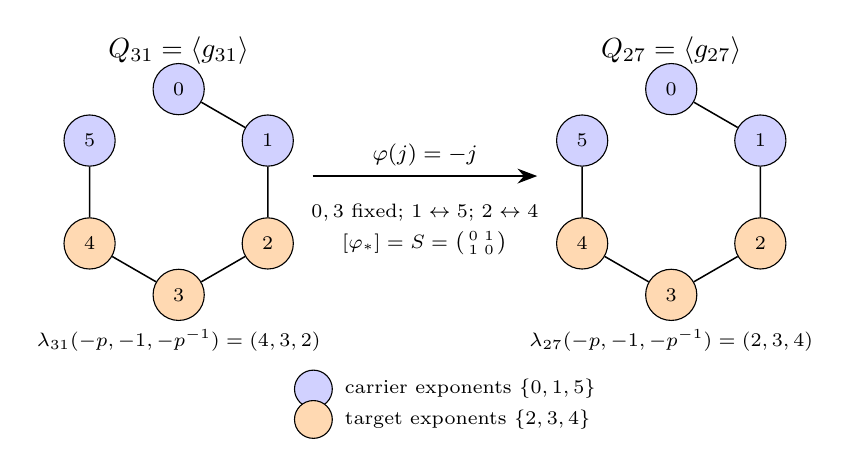
\begin{tikzpicture}[
  scale=0.92,
  every node/.style={font=\small},
  qnode/.style={circle,draw=black,minimum size=6.5mm,inner sep=0pt,
                font=\scriptsize},
  carrier/.style={qnode,fill=blue!18},
  target/.style={qnode,fill=orange!30},
  maparrow/.style={-{Stealth[length=2.5mm]},line width=0.8pt}
]
\coordinate (L) at (-3.4,0);
\coordinate (R) at ( 3.4,0);

\node[carrier] (L0) at ($(L)+(90:1.42)$)  {0};
\node[carrier] (L1) at ($(L)+(30:1.42)$)  {1};
\node[target]  (L2) at ($(L)+(-30:1.42)$) {2};
\node[target]  (L3) at ($(L)+(-90:1.42)$) {3};
\node[target]  (L4) at ($(L)+(-150:1.42)$){4};
\node[carrier] (L5) at ($(L)+(150:1.42)$) {5};
\draw[line width=0.55pt]
  (L0)--(L1)--(L2)--(L3)--(L4)--(L5)--cycle;

\node[carrier] (R0) at ($(R)+(90:1.42)$)  {0};
\node[carrier] (R1) at ($(R)+(30:1.42)$)  {1};
\node[target]  (R2) at ($(R)+(-30:1.42)$) {2};
\node[target]  (R3) at ($(R)+(-90:1.42)$) {3};
\node[target]  (R4) at ($(R)+(-150:1.42)$){4};
\node[carrier] (R5) at ($(R)+(150:1.42)$) {5};
\draw[line width=0.55pt]
  (R0)--(R1)--(R2)--(R3)--(R4)--(R5)--cycle;

\node[font=\bfseries] at ($(L)+(0,1.95)$) {$Q_{31}=\langle g_{31}\rangle$};
\node[font=\bfseries] at ($(R)+(0,1.95)$) {$Q_{27}=\langle g_{27}\rangle$};
\node[align=center,font=\scriptsize] at ($(L)+(0,-2.05)$)
  {$\lambda_{31}(-p,-1,-p^{-1})=(4,3,2)$};
\node[align=center,font=\scriptsize] at ($(R)+(0,-2.05)$)
  {$\lambda_{27}(-p,-1,-p^{-1})=(2,3,4)$};

\draw[maparrow] (-1.55,0.22) -- (1.55,0.22)
  node[midway,above,font=\footnotesize] {$\varphi(j)=-j$};
\node[align=center,font=\scriptsize] at (0,-0.52)
  {$0,3$ fixed; $1\leftrightarrow5$; $2\leftrightarrow4$\\[1mm]
   $[\varphi_*]=S=\left(\begin{smallmatrix}0&1\\1&0\end{smallmatrix}\right)$};

\node[carrier,minimum size=4.8mm] at (-1.54,-2.72) {};
\node[anchor=west,font=\scriptsize] at (-1.24,-2.72)
  {carrier exponents $\{0,1,5\}$};
\node[target,minimum size=4.8mm] at (-1.54,-3.14) {};
\node[anchor=west,font=\scriptsize] at (-1.24,-3.14)
  {target exponents $\{2,3,4\}$};
\end{tikzpicture}
\caption{The ordered adjacent-shell quotient channel.  Exponent inversion is
the unique group isomorphism carrying the three ordered origins at \(R=31\)
to their corresponding origins at \(R=27\).  On the carrier endpoints it is
the exchange matrix \(S\), and conjugation by the same matrix exchanges
\(2E_{21}\) with \(2E_{12}\).}
\label{fig:adjacent-c6-origin-inversion}
\end{figure}

\begin{corollary}[Logarithmic selection of the ordered blade basis]
\label{cor:adjacent-logarithmic-blade-selector}
In the six shells of
\cref{prop:adjacent-ordered-origin-inversion}, put
\[
 q_{31}=3,
 \qquad
 q_{27}=5,
 \qquad
 u_{R,+}=a_Rq_R,
 \qquad
 u_{R,-}=a_R/q_R.
\]
Then
\begin{equation}
 u_{R,+}u_{R,-}=a_R^2,
 \qquad
 \frac{u_{R,+}}{a_R}=q_R,
 \qquad
 \frac{u_{R,-}}{a_R}=q_R^{-1}.
 \label{eq:adjacent-complementary-carrier-representatives}
\end{equation}
In particular, \(u_{R,+}\) and \(u_{R,-}\) are complementary divisors of
\(a_R^2\) representing the exponent endpoints \(+1\) and \(-1\).

Define the arithmetic logarithmic operator on \(V_R\) by
\begin{equation}
 \mathcal L_Re_{R,+}=(\log q_R)e_{R,+},
 \qquad
 \mathcal L_Re_{R,-}=-(\log q_R)e_{R,-}.
 \label{eq:adjacent-arithmetic-logarithmic-operator}
\end{equation}
There is a unique bijection from the endpoint basis
\(\{e_{R,+},e_{R,-}\}\) to the ordered blade basis
\(\{2E_{21},2E_{12}\}\) whose linear extension intertwines
\(\mathcal L_R\) with the maintained modular Hamiltonian
\(\widetilde K_{q_R}\).  It is
\begin{equation}
 \Theta_R(e_{R,+})=2E_{12},
 \qquad
 \Theta_R(e_{R,-})=2E_{21},
 \qquad
 \Theta_R\mathcal L_R=\widetilde K_{q_R}\Theta_R.
 \label{eq:adjacent-unique-logarithmic-blade-selector}
\end{equation}
For the cross-shell maps of
\cref{prop:adjacent-ordered-origin-inversion},
\begin{align}
 \Theta_{27}\varphi_*
 &=\sigma_{\mathrm{bl}}\Theta_{31},
 \label{eq:adjacent-selected-cross-shell-intertwiner}\\
 \mathcal L_{27}\varphi_*
 &=-\frac{\log5}{\log3}\,
   \varphi_*\mathcal L_{31},
 \label{eq:adjacent-arithmetic-log-antiintertwiner}\\
 \widetilde K_5\sigma_{\mathrm{bl}}
 &=-\frac{\log5}{\log3}\,
   \sigma_{\mathrm{bl}}\widetilde K_3.
 \label{eq:adjacent-blade-log-antiintertwiner}
\end{align}
\end{corollary}

\begin{proof}
The local quotient-image table in the proof of
\cref{prop:adjacent-ordered-origin-inversion} has exactly one nontrivial
factor in each shell: \(3\) for \(R=31\) and \(5\) for \(R=27\).  Each has
valuation one in \(a_R\).  Hence the two integers in
\eqref{eq:adjacent-complementary-carrier-representatives} divide \(a_R^2\),
their product is \(a_R^2\), and their quotient logs are \(+1\) and \(-1\).
This proves \eqref{eq:adjacent-complementary-carrier-representatives} and
\eqref{eq:adjacent-arithmetic-logarithmic-operator}.

Equation \eqref{eq:ordered-sheet-modular-signs}, with
\(\lambda=q_R\), gives
\[
 \widetilde K_{q_R}(2E_{21})
 =-(\log q_R)(2E_{21}),
 \qquad
 \widetilde K_{q_R}(2E_{12})
 = (\log q_R)(2E_{12}).
\]
The two eigenvalues are distinct.  Eigenvalue preservation therefore sends
\(e_{R,+}\) to \(2E_{12}\) and \(e_{R,-}\) to \(2E_{21}\), proving existence
and uniqueness in \eqref{eq:adjacent-unique-logarithmic-blade-selector}.

Relative to the endpoint basis and the ordered blade basis
\((2E_{21},2E_{12})\), both \([\varphi_*]\) and
\([\sigma_{\mathrm{bl}}]\) are the exchange matrix \(S\), while
\([\Theta_R]=S\).  This proves
\eqref{eq:adjacent-selected-cross-shell-intertwiner}.  Applying the remaining
two identities to the two basis vectors gives
\eqref{eq:adjacent-arithmetic-log-antiintertwiner} and
\eqref{eq:adjacent-blade-log-antiintertwiner}.
\end{proof}

\begin{theorem}[CRT and kernel-generation criterion for adjacent inversion]
\label{thm:adjacent-inversion-criterion}
Let \(p\) be a prime with \(p\equiv1\pmod4\), and put
\[
 a_R=\frac{p+R}{4}
 \qquad(R\in\{31,27\}).
\]
Retain \(K_{31},K_{27},g_{31},g_{27}\) and the logarithms
\(\lambda_{31},\lambda_{27}\) from
\cref{prop:adjacent-ordered-origin-inversion}.  Define
\[
 \rho_R:=\lambda_R(pK_R).
\]
Then the ordered target has the general exponent formula
\begin{equation}
 \bigl(
 \lambda_R(-pK_R),
 \lambda_R(-K_R),
 \lambda_R(-p^{-1}K_R)
 \bigr)
 =
 (3+\rho_R,3,3-\rho_R)
 \quad\text{in }(\mathbb Z/6\mathbb Z)^3.
 \label{eq:adjacent-general-target-exponents}
\end{equation}
Consequently, the ordered transition
\[
 (4,3,2)\quad\longmapsto\quad(2,3,4)
\]
occurs exactly when
\begin{equation}
 p\bmod31\in3K_{31}=\{3,6,12,17,24\},
 \qquad
 p\bmod27\in2K_{27}=\{2,11,20\}.
 \label{eq:adjacent-target-coset-criterion}
\end{equation}
Together with \(p\equiv1\pmod4\), these are the fifteen residue classes
\begin{equation}
\begin{split}
 \mathcal R_{31,27}=\{&
 65,353,389,533,1109,1181,1469,1505,1649,\\
 &2225,2297,2585,2621,2765,3341\}
 \pmod{3348}.
\end{split}
 \label{eq:adjacent-target-CRT-classes}
\end{equation}
Every class in \(\mathcal R_{31,27}\) is coprime to \(3348\); hence every
class contains infinitely many primes.

For the factorization
\[
 a_R=\prod_{\ell}\ell^{e_{\ell,R}},
\]
put
\begin{equation}
 I_{\ell,R}
 :=\{j\lambda_R(\ell K_R):
       -e_{\ell,R}\le j\le e_{\ell,R}\}
 \subseteq\mathbb Z/6\mathbb Z.
 \label{eq:adjacent-local-factor-exponent-set}
\end{equation}
The shell carrier satisfies
\begin{equation}
 \lambda_R(B_R/K_R)
 =
 \sum_{\ell\mid a_R}I_{\ell,R}.
 \label{eq:adjacent-carrier-factor-sum}
\end{equation}
Assume \eqref{eq:adjacent-target-coset-criterion}.  The \(R\)-shell has
stabilizer \(K_R\) and is a zero-defect failure exactly when
\begin{equation}
 \sum_{\ell\mid a_R}I_{\ell,R}=\{0,1,5\},
 \qquad
 K_RB_R=B_R.
 \label{eq:adjacent-exact-carrier-criterion}
\end{equation}

The exact carrier criterion has the following factor-level formulation.  Put
\[
 q_{31}=3,
 \qquad
 q_{27}=5,
\]
and assume
\begin{equation}
 e_{q_R,R}=1,
 \qquad
 \ell K_R=K_R
 \quad
 (\ell\mid a_R, \ell\ne q_R).
 \label{eq:adjacent-single-active-factor}
\end{equation}
Define the kernel carrier
\begin{equation}
 C_R:=
 \prod_{\substack{\ell^{e_{\ell,R}}\Vert a_R\\\ell\ne q_R}}
 \{\ell^j:-e_{\ell,R}\le j\le e_{\ell,R}\}.
 \label{eq:adjacent-kernel-carrier}
\end{equation}
Under \eqref{eq:adjacent-single-active-factor},
\begin{equation}
 \eqref{eq:adjacent-exact-carrier-criterion}
 \quad\Longleftrightarrow\quad
 C_R=K_R.
 \label{eq:adjacent-kernel-generation-equivalence}
\end{equation}
\end{theorem}

\begin{proof}
Since \(-1\) has exponent \(3\) in both cyclic quotients, multiplication by
\(-1\), \(p\), and \(p^{-1}\) gives
\eqref{eq:adjacent-general-target-exponents}.  The two desired triples are
equivalent to
\[
 \rho_{31}=1,
 \qquad
 \rho_{27}=-1.
\]
The first equality is \(pK_{31}=3K_{31}\).  The second is
\(pK_{27}=g_{27}^{-1}=2K_{27}\).  This proves
\eqref{eq:adjacent-target-coset-criterion}.  The Chinese remainder theorem
gives the list in \eqref{eq:adjacent-target-CRT-classes}.  Direct gcd
calculation shows that all fifteen representatives are coprime to \(3348\);
the infinitude statement follows from Dirichlet's theorem on primes in
arithmetic progressions.

Every divisor \(u\mid a_R^2\) has a unique exponent presentation
\[
 u=\prod_{\ell\mid a_R}\ell^{e_{\ell,R}+j_\ell},
 \qquad
 -e_{\ell,R}\le j_\ell\le e_{\ell,R}.
\]
After division by \(a_R\) and passage to \(Q_R\), this gives
\eqref{eq:adjacent-carrier-factor-sum}.  Under the target criterion, the
target exponent set is \(U=\{2,3,4\}\).  Suppose first that the two
conditions in \eqref{eq:adjacent-exact-carrier-criterion} hold.  The carrier
image is the complementary set \(C=\{0,1,5\}\), so the shell fails.  The
translation stabilizer of \(C\) in \(\mathbb Z/6\mathbb Z\) is trivial.
Since \(B_R\) is \(K_R\)-stable, its full stabilizer is therefore exactly
\(K_R\).

Write \(a_{\ell}(K_R)=|I_{\ell,R}|\).  The equality \(|C|=3\) forces
\[
 \sum_{\ell\mid a_R}\bigl(a_{\ell}(K_R)-1\bigr)\geq2:
\]
if the sum were at most one, the quotient carrier would have at most two
elements.  Hence \(\kappa(K_R)\geq3\).  Kneser's bound gives
\(\kappa(K_R)\leq|C|=3\), and consequently
\[
 \kappa(K_R)=3,
 \qquad
 \delta_{K_R}=6-3-3=0,
 \qquad
 \epsilon_{K_R}=3-3=0.
\]
Thus the failure has zero defect.  Conversely, if the shell has stabilizer
\(K_R\) and is a zero-defect failure, the exact defect theorem gives
\(Q_R=C\mathbin{\dot\cup}U\).  Since \(U=\{2,3,4\}\), one has
\(C=\{0,1,5\}\), while \(K_RB_R=B_R\) follows from the stabilizer
assumption.  This proves \eqref{eq:adjacent-exact-carrier-criterion}.

Under \eqref{eq:adjacent-single-active-factor}, every local factor other than
\(q_R\) lies inside \(K_R\), while \(q_RK_R=g_R\) and
\(e_{q_R,R}=1\).  Therefore
\[
 B_R=\{q_R^{-1},1,q_R\}C_R.
\]
The three factors on the right lie in three distinct \(K_R\)-cosets.  Thus
\(B_R\) is \(K_R\)-stable exactly when the nonempty subset
\(C_R\subseteq K_R\) is \(K_R\)-stable.  Left multiplication of \(K_R\) on
itself is transitive, so this occurs exactly when \(C_R=K_R\).  The quotient
image is then \(\{0,1,5\}\), proving
\eqref{eq:adjacent-kernel-generation-equivalence}.
\end{proof}

\begin{corollary}[Prime-order internal kernel weights]
\label{cor:adjacent-prime-order-kernel-weights}
Assume \eqref{eq:adjacent-single-active-factor}.  Put
\[
 n_{31}=5,
 \qquad
 h_{31}=2,
 \qquad
 n_{27}=3,
 \qquad
 h_{27}=10,
\]
and let
\[
 \mu_R:K_R\longrightarrow\mathbb Z/n_R\mathbb Z,
 \qquad
 \mu_R(h_R^j)=j.
\]
Define the internal kernel weight
\begin{equation}
 w_R
 :=
 \sum_{\substack{\ell^{e_{\ell,R}}\Vert a_R,\ \ell\ne q_R\\
                  \mu_R(\ell)\ne0}}
 e_{\ell,R}.
 \label{eq:adjacent-internal-kernel-weight}
\end{equation}
Then
\begin{equation}
 C_{31}=K_{31}
 \quad\Longleftrightarrow\quad
 w_{31}\ge2,
 \qquad
 C_{27}=K_{27}
 \quad\Longleftrightarrow\quad
 w_{27}\ge1.
 \label{eq:adjacent-prime-order-kernel-thresholds}
\end{equation}
Consequently, under the ordered-target and single-active-factor conditions,
both adjacent shells have full zero-defect support exactly when the two
inequalities in \eqref{eq:adjacent-prime-order-kernel-thresholds} hold.
\end{corollary}

\begin{proof}
For each kernel factor, put
\[
 J_{\ell,R}
 :=
 \{j\mu_R(\ell):-e_{\ell,R}\le j\le e_{\ell,R}\}
 \subseteq\mathbb Z/n_R\mathbb Z.
\]
Applying \(\mu_R\) to \eqref{eq:adjacent-kernel-carrier} gives
\begin{equation}
 \mu_R(C_R)
 =
 \sum_{\substack{\ell^{e_{\ell,R}}\Vert a_R\\\ell\ne q_R}}
 J_{\ell,R}.
 \label{eq:adjacent-internal-kernel-sumset}
\end{equation}

For \(R=27\), every nonzero \(\alpha\in\mathbb Z/3\mathbb Z\) satisfies
\[
 \{-\alpha,0,\alpha\}=\mathbb Z/3\mathbb Z.
\]
Thus the sumset in \eqref{eq:adjacent-internal-kernel-sumset} is the whole
group exactly when at least one kernel factor has nonzero internal log.  This
is \(w_{27}\ge1\).

For \(R=31\), weight zero gives the singleton \(\{0\}\), and weight one
gives one three-element set \(\{-\alpha,0,\alpha\}\).  Suppose
\(w_{31}\ge2\).  If one active factor has valuation at least two, its local
set contains
\[
 \{-2\alpha,-\alpha,0,\alpha,2\alpha\}
 =\mathbb Z/5\mathbb Z.
\]
Otherwise there are two active valuation-one factors with nonzero logs
\(\alpha\) and \(\beta\).  After multiplication by \(\alpha^{-1}\), the
second log is one of \(\pm1\) or \(\pm2\).  Direct addition gives
\[
 \{0,\pm1\}+\{0,\pm1\}=\mathbb Z/5\mathbb Z,
 \qquad
 \{0,\pm1\}+\{0,\pm2\}=\mathbb Z/5\mathbb Z.
\]
Additional local sets preserve the full group.  Hence
\(C_{31}=K_{31}\) exactly when \(w_{31}\ge2\).  The last assertion follows
from \cref{thm:adjacent-inversion-criterion}.
\end{proof}

\begin{corollary}[Residue-factor criterion for full adjacent support]
\label{cor:adjacent-residue-factor-criterion}
Assume the ordered-target and single-active-factor conditions of
\cref{thm:adjacent-inversion-criterion}.  Define
\begin{align}
 \nu_{31}^{\mathrm{nt}}(a_{31})
 &:={}
 \sum_{\substack{\ell^e\Vert a_{31}\\
                   \ell\bmod31\in\{2,4,8,16\}}} e,
 \label{eq:adjacent-residue-weight-31}\\
 \nu_{27}^{\mathrm{nt}}(a_{27})
 &:={}
 \sum_{\substack{\ell^e\Vert a_{27}\\
                   \ell\bmod27\in\{10,19\}}} e.
 \label{eq:adjacent-residue-weight-27}
\end{align}
Then
\begin{align}
 C_{31}=K_{31}
 &\quad\Longleftrightarrow\quad
 \nu_{31}^{\mathrm{nt}}(a_{31})\ge2,
 \label{eq:adjacent-residue-kernel-31}\\
 C_{27}=K_{27}
 &\quad\Longleftrightarrow\quad
 \nu_{27}^{\mathrm{nt}}(a_{27})\ge1.
 \label{eq:adjacent-residue-kernel-27}
\end{align}
Consequently, the two adjacent shells have full zero-defect support exactly
when both inequalities hold.
\end{corollary}

\begin{proof}
The internal logarithm \(\mu_{31}\) has kernel \(\{1\}\) on
\[
 K_{31}=\{1,2,4,8,16\},
\]
so its nonzero values occur exactly on the residue classes
\(2,4,8,16\pmod{31}\).  Likewise, \(\mu_{27}\) has kernel \(\{1\}\) on
\[
 K_{27}=\{1,10,19\},
\]
so its nonzero values occur exactly on the residue classes
\(10,19\pmod{27}\).  The single-active-factor conditions place every
kernel factor in the corresponding subgroup.  Therefore
\[
 \nu_{31}^{\mathrm{nt}}(a_{31})=w_{31},
 \qquad
 \nu_{27}^{\mathrm{nt}}(a_{27})=w_{27}.
\]
The result follows from
\cref{cor:adjacent-prime-order-kernel-weights}.
\end{proof}

\begin{corollary}[Consecutive-integer form of the adjacent criterion]
\label{cor:adjacent-consecutive-integer-criterion}
Let \(p\) satisfy the ordered-target conditions
\eqref{eq:adjacent-target-coset-criterion}, and put
\[
 a:=a_{31}=\frac{p+31}{4}.
\]
Then
\begin{equation}
 a_{27}=a-1,
 \qquad
 p=4a-31,
 \label{eq:adjacent-consecutive-parameters}
\end{equation}
and the ordered-target conditions are equivalent to
\begin{equation}
 a\bmod31\in3K_{31},
 \qquad
 a\bmod27\in1+5K_{27}=\{6,15,24\}.
 \label{eq:adjacent-consecutive-target-cosets}
\end{equation}
Equivalently,
\begin{equation}
 a\bmod837\in\mathcal A_{31,27},
 \label{eq:adjacent-consecutive-CRT-classes}
\end{equation}
where
\[
\begin{split}
 \mathcal A_{31,27}=\{&
 6,24,96,105,141,285,303,375,384,\\
 &420,564,582,654,663,699\}.
\end{split}
\]
Every such \(a\) satisfies
\begin{equation}
 a\equiv6\pmod9,
 \qquad
 v_3(a)=1.
 \label{eq:adjacent-consecutive-three-valuation}
\end{equation}
Furthermore,
\begin{equation}
 v_5(a-1)=1
 \quad\Longleftrightarrow\quad
 p\bmod100\in\{13,33,53,93\}.
 \label{eq:adjacent-consecutive-five-valuation}
\end{equation}

On the ordered-target locus, the single-active-factor conditions
\eqref{eq:adjacent-single-active-factor} therefore hold exactly when
\eqref{eq:adjacent-consecutive-five-valuation} holds and
\begin{align}
 \ell\mid a/3
 &\quad\Longrightarrow\quad
 \ell\bmod31\in\{1,2,4,8,16\},
 \label{eq:adjacent-consecutive-factor-31}\\
 \ell\mid(a-1)/5
 &\quad\Longrightarrow\quad
 \ell\bmod27\in\{1,10,19\}
 \label{eq:adjacent-consecutive-factor-27}
\end{align}
for every prime \(\ell\).  Under these conditions, both shells have full
zero-defect support exactly when
\begin{align}
 \sum_{\substack{\ell^e\Vert a/3\\
                   \ell\bmod31\in\{2,4,8,16\}}}e
 &\ge2,
 \label{eq:adjacent-consecutive-weight-31}\\
 \sum_{\substack{\ell^e\Vert(a-1)/5\\
                   \ell\bmod27\in\{10,19\}}}e
 &\ge1.
 \label{eq:adjacent-consecutive-weight-27}
\end{align}
\end{corollary}

\begin{proof}
The identities in \eqref{eq:adjacent-consecutive-parameters} follow directly
from the definitions of \(a_{31}\) and \(a_{27}\).  Modulo \(31\), one has
\(p=4a\) and \(4\in K_{31}\), so
\[
 pK_{31}=3K_{31}
 \quad\Longleftrightarrow\quad
 aK_{31}=3K_{31}.
\]
Modulo \(27\), one has \(p=4(a-1)\).  Since
\[
 4(5K_{27})=20K_{27}=2K_{27},
\]
the second target condition is equivalent to
\((a-1)K_{27}=5K_{27}\), which is the second statement in
\eqref{eq:adjacent-consecutive-target-cosets}.  The Chinese remainder theorem
then gives the fifteen classes in
\eqref{eq:adjacent-consecutive-CRT-classes}.

The three residues \(6,15,24\pmod{27}\) are all congruent to
\(6\pmod9\).
This proves \eqref{eq:adjacent-consecutive-three-valuation}.  Since
\[
 4(a-1)=p+27,
\]
the condition \(v_5(a-1)=1\) is equivalent to
\[
 p+27\bmod100\in\{20,40,60,80\},
\]
which gives \eqref{eq:adjacent-consecutive-five-valuation}.

Equation \eqref{eq:adjacent-consecutive-three-valuation} supplies the exact
valuation of the distinguished factor \(3\).  Equation
\eqref{eq:adjacent-consecutive-five-valuation} supplies the exact valuation
of the distinguished factor \(5\).  The remaining clauses of
\eqref{eq:adjacent-single-active-factor} say precisely that the prime factors
of \(a/3\) and \((a-1)/5\) lie in \(K_{31}\) and \(K_{27}\),
respectively.
This proves
\eqref{eq:adjacent-consecutive-factor-31}--
\eqref{eq:adjacent-consecutive-factor-27}.  Finally,
\eqref{eq:adjacent-consecutive-weight-31}--
\eqref{eq:adjacent-consecutive-weight-27} are the residue weights from
\cref{cor:adjacent-residue-factor-criterion} after removing the distinguished
 factors.
\end{proof}

\begin{corollary}[Exact Diophantine cofactor parameterization]
\label{cor:adjacent-Diophantine-cofactor-parameterization}
Let \(p\) be a positive prime.  The following statements are equivalent.
\begin{enumerate}[label=\textup{(\roman*)}]
\item The prime \(p\) satisfies the ordered-target conditions
\eqref{eq:adjacent-target-coset-criterion} and the single-active-factor
conditions \eqref{eq:adjacent-single-active-factor} for the adjacent
\(R=31\) and \(R=27\) shells.
\item There is a unique integer \(t\geq1\) such that
\begin{equation}
 p=60t-7,
 \qquad
 b:=5t+2,
 \qquad
 c:=3t+1,
 \label{eq:adjacent-Diophantine-t-parameters}
\end{equation}
and every prime divisor of \(b\) belongs modulo \(31\) to
\(K_{31}=\{1,2,4,8,16\}\), while every prime divisor of \(c\) belongs
modulo \(27\) to \(K_{27}=\{1,10,19\}\).
\end{enumerate}
Under these equivalent conditions,
\begin{equation}
 a:=\frac{p+31}{4}=15t+6=3b=5c+1,
 \label{eq:adjacent-Diophantine-consecutive-factors}
\end{equation}
and the two shells have full zero-defect support exactly when
\begin{align}
 \omega_{31}(b)
 &:={}
 \sum_{\substack{\ell^e\Vert b\\
                   \ell\bmod31\in\{2,4,8,16\}}}e
 \geq2,
 \label{eq:adjacent-Diophantine-weight-31}\\
 \omega_{27}(c)
 &:={}
 \sum_{\substack{\ell^e\Vert c\\
                   \ell\bmod27\in\{10,19\}}}e
 \geq1.
 \label{eq:adjacent-Diophantine-weight-27}
\end{align}
For every \(t\geq1\) for which \(60t-7\) is prime, the ordered-target
conditions alone are equivalent to
\begin{equation}
 t\bmod93\in\{0,6,9,57,81\}.
 \label{eq:adjacent-Diophantine-target-t-classes}
\end{equation}
\end{corollary}

\begin{proof}
Assume (i), and put \(a=(p+31)/4\).  The ordered-target condition gives
\(a\equiv6\pmod9\), hence \(3\mid a\) and \(v_3(a)=1\), by
\eqref{eq:adjacent-consecutive-three-valuation}.  The
single-active-factor condition gives \(v_5(a-1)=1\).  Therefore
\(a\equiv0\pmod3\) and \(a\equiv1\pmod5\), so there is a unique integer
\(t\) with
\[
 a=15t+6.
\]
Since \(p=4a-31>0\), one has \(t\geq1\).  Direct substitution gives
\eqref{eq:adjacent-Diophantine-t-parameters} and
\eqref{eq:adjacent-Diophantine-consecutive-factors}.  The prime-divisor
conditions in (ii) are precisely
\eqref{eq:adjacent-consecutive-factor-31} and
\eqref{eq:adjacent-consecutive-factor-27} with
\(b=a/3\) and \(c=(a-1)/5\).

Conversely, assume (ii) and define \(a\) by
\eqref{eq:adjacent-Diophantine-consecutive-factors}.  Products of elements
of \(K_{31}\) and \(K_{27}\) remain in the respective subgroups, so
\[
 b\bmod31\in K_{31},
 \qquad
 c\bmod27\in K_{27}.
\]
Consequently
\[
 aK_{31}=3K_{31},
 \qquad
 (a-1)K_{27}=5K_{27}.
\]
Equation \eqref{eq:adjacent-consecutive-target-cosets} proves the
ordered-target conditions.  Since \(3\bmod31\notin K_{31}\), the stated
condition on the prime divisors of \(b\) gives \(3\nmid b\), and hence
\(v_3(a)=1\).  Since \(5\bmod27\notin K_{27}\), the stated condition on
the prime divisors of \(c\) gives \(5\nmid c\), and hence
\(v_5(a-1)=1\).  The consecutive-factor characterization
\eqref{eq:adjacent-consecutive-factor-31}--
\eqref{eq:adjacent-consecutive-factor-27} now proves the
single-active-factor conditions.

For the final residue assertion, write \(a=15t+6\),
\(b=5t+2\), and \(c=3t+1\).  The ordered-target conditions are
equivalent to
\[
 b\bmod31\in K_{31},
 \qquad
 c\bmod27\in K_{27}.
\]
Since \(5^{-1}\equiv25\pmod{31}\), the first condition gives
\[
 t\bmod31\in\{0,6,9,19,26\}.
\]
The second condition is equivalent to \(t\equiv0\pmod3\).  Applying the
Chinese remainder theorem modulo \(3\cdot31=93\) gives exactly
\[
 t\bmod93\in\{0,6,9,57,81\},
\]
which proves \eqref{eq:adjacent-Diophantine-target-t-classes}.

Finally, substituting \(b=a/3\) and \(c=(a-1)/5\) into
\eqref{eq:adjacent-consecutive-weight-31}--
\eqref{eq:adjacent-consecutive-weight-27} gives
\eqref{eq:adjacent-Diophantine-weight-31}--
\eqref{eq:adjacent-Diophantine-weight-27} and proves the full-support
criterion.
\end{proof}

\begin{corollary}[Sixfold parameter and the modulus-\(360\) prime line]
\label{cor:adjacent-sixfold-u-parameterization}
Under the equivalent conditions of
\cref{cor:adjacent-Diophantine-cofactor-parameterization}, the parameter
\(t\) is divisible by \(6\).  Thus there is a unique integer \(u\geq1\)
such that
\begin{equation}
 t=6u,
 \qquad
 p=360u-7,
 \qquad
 a=90u+6,
 \label{eq:adjacent-sixfold-u-prime-line}
\end{equation}
and
\begin{equation}
 \frac a3=30u+2=2(15u+1),
 \qquad
 \frac{a-1}{5}=18u+1.
 \label{eq:adjacent-sixfold-u-cofactors}
\end{equation}
In particular,
\begin{equation}
 p\equiv353\pmod{360}.
 \label{eq:adjacent-single-active-mod360}
\end{equation}

For every \(u\geq1\) for which \(360u-7\) is prime, the ordered-target
conditions alone are equivalent to
\begin{equation}
 u\bmod31\in\{0,1,17,25,29\}.
 \label{eq:adjacent-u-target-classes}
\end{equation}
On the ordered single-active locus, full support is equivalent to
\begin{align}
 \sum_{\substack{\ell^e\Vert 2(15u+1)\\
                   \ell\bmod31\in\{2,4,8,16\}}}e
 &\geq2,
 \label{eq:adjacent-u-weight-31}\\
 \sum_{\substack{\ell^e\Vert 18u+1\\
                   \ell\bmod27\in\{10,19\}}}e
 &\geq1.
 \label{eq:adjacent-u-weight-27}
\end{align}
\end{corollary}

\begin{proof}
The single-active-factor condition requires every prime divisor of
\(c=3t+1\) to lie in \(K_{27}\).  Since
\(2\bmod27\notin K_{27}\), the integer \(c\) is odd.  Hence \(t\) is even.
Equation \eqref{eq:adjacent-Diophantine-target-t-classes} gives
\(3\mid t\), so \(t=6u\) for a unique integer \(u\geq1\).
Substitution proves
\eqref{eq:adjacent-sixfold-u-prime-line}--%
\eqref{eq:adjacent-single-active-mod360}.

For the target criterion, the residue modulo \(27\) is
\[
 a=90u+6\equiv9u+6\pmod{27},
\]
which always belongs to \(\{6,15,24\}=1+5K_{27}\).  Modulo \(31\),
\[
 a=3(30u+2)\equiv3(2-u)\pmod{31}.
\]
Therefore \(a\bmod31\in3K_{31}\) exactly when
\[
 u\bmod31\in2-K_{31}
 =\{0,1,17,25,29\}.
\]
This proves \eqref{eq:adjacent-u-target-classes}.  The two weight statements
follow by substituting \eqref{eq:adjacent-sixfold-u-cofactors} into
\eqref{eq:adjacent-Diophantine-weight-31}--%
\eqref{eq:adjacent-Diophantine-weight-27}.
\end{proof}

\begin{corollary}[Power-of-two/odd-prime cofactor family]
\label{cor:adjacent-binary-prime-cofactor-family}
Let \(m\geq1\), let \(r\) be either \(1\) or an odd prime, and put
\[
 a=3\cdot2^m r.
\]
Assume
\begin{align}
 r\bmod31&\in K_{31}=\{1,2,4,8,16\},
 \label{eq:adjacent-cofactor-r31}\\
 a-1&=5q
 \quad\text{for a prime }q\text{ with }
 q\bmod27\in\{10,19\},
 \label{eq:adjacent-cofactor-q27}\\
 p&=4a-31
 \quad\text{is prime}.
 \label{eq:adjacent-cofactor-p}
\end{align}
Define
\[
 \varepsilon_{31}(r)=
 \begin{cases}
  0,&r\equiv1\pmod{31},\\
  1,&r\bmod31\in\{2,4,8,16\}.
 \end{cases}
\]
If
\begin{equation}
 m+\varepsilon_{31}(r)\geq2,
 \label{eq:adjacent-cofactor-weight}
\end{equation}
then \(p\) satisfies the ordered adjacent transition
\[
 (4,3,2)\longmapsto(2,3,4),
\]
and both the \(R=31\) and \(R=27\) shells have full zero-defect
support.
\end{corollary}

\begin{proof}
Equation~\eqref{eq:adjacent-cofactor-p} gives \(p\equiv1\pmod4\).
Modulo \(31\), equations
\eqref{eq:adjacent-cofactor-r31} and \(2\in K_{31}\) give
\[
 a=3\cdot2^m r\in3K_{31}.
\]
Modulo \(27\), equation~\eqref{eq:adjacent-cofactor-q27} gives
\[
 a=1+5q\in1+5K_{27}.
\]
Hence the ordered-target criterion
\eqref{eq:adjacent-consecutive-target-cosets} holds.

The two consecutive factors are
\[
 \frac a3=2^m r,
 \qquad
 \frac{a-1}{5}=q.
\]
Every prime factor of \(a/3\) lies in \(K_{31}\), and its
nontrivial internal-log weight is exactly
\(m+\varepsilon_{31}(r)\).  Every prime factor of \((a-1)/5\) lies
in \(K_{27}\), and its nontrivial internal-log weight is exactly one
because \(q\bmod27\in\{10,19\}\).  Thus
\eqref{eq:adjacent-consecutive-factor-31}--%
\eqref{eq:adjacent-consecutive-factor-27} and
\eqref{eq:adjacent-consecutive-weight-31}--%
\eqref{eq:adjacent-consecutive-weight-27} all hold.  The conclusion follows
from \cref{cor:adjacent-consecutive-integer-criterion}.
\end{proof}

\begin{computation}[Bounded adjacent-inversion criterion]
The exact script and captured receipt
\begin{center}
\texttt{verification/verify\_adjacent\_inversion\_criterion.py},\\
\texttt{verification/verify\_adjacent\_inversion\_criterion\_output.txt}
\end{center}
verify the fifteen CRT classes and all primes \(p\le500000\).  There are
\(566\) target-compatible primes in this range.  Fourteen satisfy the
quotient-level factor condition, and exactly the following eleven also
generate both full kernels:
\[
\begin{split}
 \{&
 353,6113,10433,28433,55793,99713,\\
 &300593,340913,368633,379433,497153\}.
\end{split}
\]
The internal-weight pairs for the other three primes are
\[
 (w_{31},w_{27})
 =
 (5,0)\text{ at }p=89633,
 \qquad
 (1,1)\text{ at }p=111593,
 \qquad
 (2,0)\text{ at }p=490313.
\]
For all fourteen quotient-factor primes, the checker also evaluates the
residue sums in \eqref{eq:adjacent-residue-weight-31} and
\eqref{eq:adjacent-residue-weight-27} and verifies their equality with
\(w_{31}\) and \(w_{27}\), respectively.
The same run enumerates the fifteen classes in
\eqref{eq:adjacent-consecutive-CRT-classes}, checks the exact
\(3\)- and \(5\)-adic valuation criteria, and verifies that the
 consecutive-factor predicate and the quotient-factor predicate agree on all
\(566\) target-compatible primes in the bounded range.
It also verifies the equivalent \(t\)-parameter criterion in
\cref{cor:adjacent-Diophantine-cofactor-parameterization} on the same
\(566\) primes.  The eleven full-support values correspond to
\[
 (t_1,\ldots,t_{11})
 =
 (6,102,174,474,930,1662,5010,5682,6144,6324,8286).
\]
Equivalently, on the sixfold line of
\cref{cor:adjacent-sixfold-u-parameterization}, they are
\[
 (u_1,\ldots,u_{11})
 =
 (1,17,29,79,155,277,835,947,1024,1054,1381).
\]
Ten of the eleven full-support primes belong to the family in
\cref{cor:adjacent-binary-prime-cofactor-family}:
\[
\begin{split}
 \{&
 353,6113,10433,28433,55793,99713,\\
 &300593,340913,368633,497153\}.
\end{split}
\]
For the remaining value \(p=379433\), one has
\[
 a=94866,
 \qquad
 \frac a3=2\cdot97\cdot163,
 \qquad
 \frac{a-1}{5}=18973,
\]
with \(97\equiv4\pmod{31}\), \(163\equiv8\pmod{31}\), and
\(18973\equiv19\pmod{27}\).  The checker verifies both the ten-member
subfamily and this remaining two-odd-prime factorization.
For all eleven primes, the checker reconstructs both arithmetic carriers,
proves that their stabilizers are \(K_{31}\) and \(K_{27}\), obtains the
ordered target triples \((4,3,2)\) and \((2,3,4)\), and exhausts the divisor
search in both shells.  Hence all twenty-two shells are exact zero-defect
failures.
\end{computation}

\begin{computation}[Adjacent ordered-origin checker]
The script and captured receipt
\begin{center}
\texttt{verification/verify\_adjacent\_ordered\_quotient\_channel.py},\\
\texttt{verification/verify\_adjacent\_ordered\_quotient\_channel\_output.txt}
\end{center}
verify the six shell factorizations, their local quotient images and
stabilizers, the absence of divisor certificates, the two ordered
three-origin log triples, uniqueness of exponent inversion, the complementary
divisor-ratio representatives, and the endpoint, blade, and logarithmic
selector matrices.
\end{computation}

\begin{computation}[Critical-family checker]
The script and captured receipt
\begin{center}
\texttt{verification/verify\_three\_origin\_critical\_family.py},\\
\texttt{verification/verify\_three\_origin\_critical\_family\_output.txt}
\end{center}
verify \(2080\) members of the cyclic family, the complete
\((p,R,a,N)=(5,7,3,15)\) shell, and the \(R=3\) decomposition of the same
prime.  They also verify both adjacent \(p=353\) shells, their local
quotient-support cardinalities, stabilizers, target cosets, and absence of a
divisor certificate.
\end{computation}

The critical family and its arithmetic realization show that vanishing of
both local defect summands is compatible with an actual failed shell.
The adjacent \(p=353\) pair also excludes the inference that the replacement
\(R\mapsto R-4\) must leave the zero-defect locus.  A global descent requires
additional arithmetic data linking more than these two local quotient
partitions.

\begin{corollary}[Residual-shell consequence]
\label{cor:star-kneser-shell}
If all star surpluses in \cref{thm:star-kneser-forcing} are positive,
then the fixed residual shell has a divisor certificate and hence an
Erd\H{o}s--Straus decomposition.
\end{corollary}

\begin{proof}
For a divisor
\[
 u=\prod_i\ell_i^{e_i+\beta_i}\mid a^2,
 \qquad -e_i\le\beta_i\le e_i,
\]
the quotient residue $\overline u\,\overline a^{-1}$ is the element
$\sum_i\beta_i\overline{\ell}_i$ of $B$.  A hit at $\overline{-1}$
is the middle origin $j=1$ in \eqref{eq:origin-resolved-support}; a hit at
$\overline{-p^{-1}}$ is the exterior origin $j=2$.  Since every $A_i$,
and hence $B$, is invariant under inversion, the opposite exterior target
$\overline{-p}$ is paired with $\overline{-p^{-1}}$.  Thus
$B\cap T\ne\varnothing$ produces a divisor counted by
\cref{thm:general-divisor-shell}.
\end{proof}

\begin{theorem}[Complete Star--Kneser certificate at $12289$]
\label{thm:12289-star-kneser}
For
\[
 p=12289,\qquad R=11,\qquad
 a=3075=3\cdot5^2\cdot41,
\]
the divisor-ratio group is $H=(\Z/11\Z)^\times\cong C_{10}$.  With
$2$ as generator and additive logarithmic coordinates,
\[
 A_3=\{0,2,8\},\qquad
 A_5=\{0,2,4,6,8\},\qquad
 A_{41}=\{0,3,7\},
\]
and
\[
 T=\{4,5\}.
\]
For the four subgroups of $C_{10}$, the complete quotient table is
\begin{equation}
\begin{array}{c|c|c|c|c|c}
|K|&|H/K|&(a_3(K),a_5(K),a_{41}(K))
&\kappa(K)&t(K)&\Sigma_T(K)\\
\hline
1&10&(3,5,3)&9&2&1\\
2&5 &(3,5,3)&9&2&6\\
5&2 &(1,1,2)&2&2&2\\
10&1&(1,1,1)&1&1&1
\end{array}
\label{eq:12289-star-kneser-table}
\end{equation}
In particular,
\[
 \min_{K\le H}\Sigma_T(K)=1,
\]
so the shell is forced positive by
\cref{thm:star-kneser-forcing}.  Its exact three-origin count is
\[
 (m_0,m_1,m_2)=(3,6,3),
 \qquad
 \Omega_{11}(12289)=12.
\]
\end{theorem}

\begin{proof}
The powers of $2$ modulo $11$ give
\[
 \log_2(3)=8,\qquad
 \log_2(5)=4,\qquad
 \log_2(41)=\log_2(8)=3.
\]
The exponent intervals for $3^1$, $5^2$, and $41^1$ therefore give the
three displayed subsets.  Moreover
\[
 p\equiv2\pmod{11},\qquad p^{-1}\equiv6\pmod{11},
\]
so
\[
 \log_2(-1)=5,\qquad \log_2(-p^{-1})=\log_2(5)=4.
\]
This proves the descriptions of $H$, the $A_i$, and $T$.

The group $C_{10}$ has one subgroup of each order $1,2,5,10$.
For the trivial subgroup, the quotient sizes are $(3,5,3)$ and
$t=2$, hence
\[
 \kappa=1+(3-1)+(5-1)+(3-1)=9,
 \qquad \Sigma_T=9+2-10=1.
\]
For the subgroup of order $2$, reduction to $C_5$ leaves the three
set sizes $(3,5,3)$ and the two target classes distinct, giving
$\Sigma_T=9+2-5=6$.  For the subgroup of order $5$, reduction to
parity gives sizes $(1,1,2)$ and two target classes, hence
\[
 \kappa=1+0+0+1=2,
 \qquad \Sigma_T=2+2-2=2.
\]
For $K=H$, all sets have one image, so
$\Sigma_T=1+1-1=1$.  This proves
\eqref{eq:12289-star-kneser-table}.

Enumerate the
$3\cdot5\cdot3=45$ signed exponent vectors
$(\beta_3,\beta_5,\beta_{41})$.  The complete fibre over the middle
target $5=\log_2(-1)$ is
\[
\begin{gathered}
(-1,-1,-1),\quad(-1,0,1),\quad(0,-2,1),\\
(0,2,-1),\quad(1,0,-1),\quad(1,1,1),
\end{gathered}
\]
while the complete fibre over the exterior target
$4=\log_2(-p^{-1})$ is
\[
 (-1,-2,0),\qquad(0,1,0),\qquad(1,-1,0).
\]
Direct reduction of
$8\beta_3+4\beta_5+3\beta_{41}$ modulo $10$ verifies every listed
vector; inspection of the finite box gives no others.  Thus the middle
count is $6$, one exterior count is $3$, and inversion gives the other
exterior count $3$.  Hence
\[
 \Omega_{11}(12289)=6+2\cdot3=12.
\]
\end{proof}

\begin{provenance}[Source of the quotient certificate]
The formulation and the $12289$ table are reconstructed from
\emph{A Star--Kneser Positivity Criterion for Residual
Erd\H{o}s--Straus Shells}, The Clankers, May 2026
\cite{ClankersStarKneser}, local source
\path{BEAVERSHINE/8/2/star_kneser_erdos_straus.tex}.
The present proof restates the finite calculation explicitly.
\end{provenance}

\begin{computation}[The complete $12289$ coefficient-space aggregate]
\label{comp:12289-complete-circle-aggregate}
The twelve exponent vectors in \cref{thm:12289-star-kneser} give six
inversion orbits.  Writing the origin labels in the first column, the complete
divisor set is
\[
\begin{array}{c|r@{\ \longleftrightarrow\ }r}
0\leftrightarrow2&615&2\,321\,925\,135\,375\\
0\leftrightarrow2&5\,125&278\,631\,016\,245\\
0\leftrightarrow2&230\,625&6\,191\,800\,361\\
1\leftrightarrow1&61\,445&23\,240\,035\,125\\
1\leftrightarrow1&2\,765\,025&516\,445\,225\\
1\leftrightarrow1&23\,041\,875&61\,973\,427
\end{array}
\]
Here $N=37\,788\,675$, and the two entries in every row have product
$N^2$.  Thus the fibres have respective cardinalities $3,6,3$.  Direct
addition gives
\[
 \sum_{d\in\mathcal D_{11,N}}d
 =2630592510468
 =12\cdot219216042539.
\]
Consequently \cref{thm:complete-shell-circle-aggregate} gives
\begin{equation}
 V(\mathcal D_{11,N})
 =12(219216042539,37788675,0,219216042539).
 \label{eq:12289-complete-circle-aggregate}
\end{equation}
The primitive Sarnak coordinates are
\[
 (T,X,Y,W)=(219216042539,37788675,0,0),
\]
and their exact norm is
\begin{equation}
 37788675^2-219216042539^2
 =-48055671878476699310896.
 \label{eq:12289-complete-circle-norm}
\end{equation}
\end{computation}

\begin{corollary}[Outcome of the Fable substitution]
Inside the singular support envelope \eqref{eq:singular-C123-envelope}, the
Fable triple is an occupied balanced element, while the $12289$ table is an
occupied closed orbit with the explicit positive certificate
\eqref{eq:12289-explicit-ES}.  The certificate settles the
Erd\H{o}s--Straus instance at $12289$ positively.
\end{corollary}

\section{Split-zero support and the exact meaning of the \texorpdfstring{$C_1$}{C1}
carrier}

Let $R$ be a nonzero commutative ring.  Define the split-zero semiring
\begin{equation}
 G(R):=R\sqcup\{\tau\},
 \qquad e:=0_R\in R\subset G(R),
 \label{eq:split-zero-def}
\end{equation}
by
\[
 r\oplus s=r+s,\qquad r\oplus\tau=r,
 \qquad \tau\oplus\tau=\tau,
\]
and
\[
 r\odot s=rs,\qquad r\odot\tau=\tau\odot r=\tau,
 \qquad \tau\odot\tau=\tau
\]
for $r,s\in R$.  Thus $\tau$ is the additive zero of $G(R)$, whereas $e$
is the supported copy of the ring zero.

\begin{proposition}[Exact two-coordinate normal form]
\label{prop:split-zero-normal-form}
There is a canonical semiring isomorphism
\[
 G(R)\cong
 D_R:=\{(r,b)\in R\times\mathbb B:b=0\Longrightarrow r=0_R\}
     =\{(0_R,0)\}\cup(R\times\{1\}),
\]
where the operations on $D_R$ are componentwise.  Under this isomorphism,
\[
 \tau\longmapsto(0_R,0),
 \qquad r\longmapsto(r,1).
\]
Consequently the maps
\[
 p_R:G(R)\to R,
 \qquad p_R(\tau)=0_R,\quad p_R(r)=r,
\]
and
\[
 \chi_R:G(R)\to\mathbb B,
 \qquad \chi_R(\tau)=0,\quad\chi_R(r)=1,
\]
are semiring homomorphisms.
\end{proposition}

\begin{proof}
The displayed map is bijective.  Componentwise operations give
\[
 (r,1)+(s,1)=(r+s,1),
 \quad (r,1)+(0,0)=(r,1),
\]
and
\[
 (r,1)(s,1)=(rs,1),
 \quad (r,1)(0,0)=(0,0),
\]
which are exactly the defining operations of $G(R)$.  The two coordinate
projections restricted to $D_R$ are therefore semiring homomorphisms.
\end{proof}

\begin{theorem}[Entrywise split pair and the full ring-null matrix fibre]
\label{thm:split-zero-matrix-pair-fibre}
For every \(n\geq1\), entrywise application of the two coordinates in
\cref{prop:split-zero-normal-form} gives a semiring isomorphism
\begin{equation}
 \Phi_n:M_n(G(R))\xrightarrow{\ \sim\ }\mathscr D_{R,n},
 \qquad
 \Phi_n(X)=\bigl(\widehat p_R(X),\widehat\chi_R(X)\bigr),
 \label{eq:split-zero-matrix-pair-map}
\end{equation}
where
\begin{equation}
 \mathscr D_{R,n}
 :=\left\{
  (A,S)\in M_n(R)\times M_n(\mathbb B):
  S_{ij}=0\Longrightarrow A_{ij}=0_R
 \right\}.
 \label{eq:split-zero-matrix-pair-image}
\end{equation}
In particular, the complete fibre over the zero amplitude matrix is
\begin{equation}
 \widehat p_R^{-1}(0_n)
 =\left\{X_S:S\in M_n(\mathbb B)\right\},
 \qquad
 \Phi_n(X_S)=(0_n,S),
 \label{eq:ring-null-matrix-Boolean-fibre}
\end{equation}
and the support coordinate identifies its induced addition and multiplication
with those of \(M_n(\mathbb B)\).  Thus a ring-null matrix retains an entire
Boolean support matrix; it is not determined by its zero amplitude.

For the directed blade matrix of
\cref{thm:split-zero-directed-blade-support}, the pair is
\begin{equation}
 \Phi_2(\widetilde N)=\bigl(2E_{21},E_{21}\bigr).
 \label{eq:directed-blade-full-split-pair}
\end{equation}
Its support \(E_{21}\) precedes the derived source and range projectors
\(E_{11}\) and \(E_{22}\).
\end{theorem}

\begin{proof}
Apply the isomorphism of \cref{prop:split-zero-normal-form} to every matrix
entry.  This gives a bijection onto
\eqref{eq:split-zero-matrix-pair-image}.  It preserves matrix addition
because Boolean addition records the union of entry supports.  For
multiplication, suppose that the \((i,j)\)-entry of the Boolean product
\(ST\) is zero.  For every \(k\), either \(S_{ik}=0\) or \(T_{kj}=0\); the
defining support condition then gives either \(A_{ik}=0\) or \(B_{kj}=0\).
Every summand \(A_{ik}B_{kj}\) therefore vanishes, so
\((AB)_{ij}=0\).  Hence the image is closed under matrix multiplication and
\eqref{eq:split-zero-matrix-pair-map} is a semiring isomorphism.

Setting the amplitude coordinate equal to \(0_n\) leaves \(S\) arbitrary,
which proves \eqref{eq:ring-null-matrix-Boolean-fibre}.  Finally,
\(\widetilde2\mapsto(2,1)\) and every absent entry maps to \((0,0)\), so the
matrix in \eqref{eq:split-zero-directed-N} maps to
\((2E_{21},E_{21})\).  The source and range statements then follow from
\(E_{12}E_{21}=E_{11}\) and \(E_{21}E_{12}=E_{22}\).
\end{proof}

\begin{theorem}[Uniqueness of the Boolean support character]
\label{thm:unique-Boolean-support-character}
For every nonzero commutative ring \(R\), the homomorphism
\[
 \chi_R:G(R)\longrightarrow\mathbb B,
 \qquad
 \chi_R(\tau)=0,
 \qquad
 \chi_R(r)=1\quad(r\in R),
\]
is the unique semiring homomorphism from \(G(R)\) to \(\mathbb B\).
Consequently its entrywise extension
\begin{equation}
 \widehat\chi_R:M_n(G(R))\longrightarrow M_n(\mathbb B)
 \label{eq:unique-entrywise-Boolean-character}
\end{equation}
is the unique matrix-semiring homomorphism induced entrywise by a scalar
map \(G(R)\to\mathbb B\).
\end{theorem}

\begin{proof}
Let \(u:G(R)\to\mathbb B\) be a semiring homomorphism.  Since \(\tau\) is
the semiring zero and \(1_R\) is the multiplicative identity,
\[
 u(\tau)=0,
 \qquad
 u(1_R)=1.
\]
Inside the supported copy of \(R\), one has
\(0_R=1_R\oplus(-1_R)\).  Hence Boolean addition gives
\[
 u(0_R)=u(1_R)+u(-1_R)=1+u(-1_R)=1.
\]
If \(u(r)=0\) for some \(r\in R\), then
\[
 1=u(0_R)=u(r0_R)=u(r)u(0_R)=0,
\]
a contradiction.  Thus \(u(r)=1\) for every supported \(r\in R\), so
\(u=\chi_R\).  Entrywise extension preserves matrix addition and matrix
multiplication because \(\chi_R\) preserves finite sums and products.  The
scalar uniqueness gives the final assertion.  This is the Boolean-character
theorem of \cite{ClankersSplitZero} in the notation used here.
\end{proof}

\begin{theorem}[Unique positive-cone lift of the axial coordinate]
\label{thm:Fable-positive-cone-split-zero-height}
Equip \(\mathbb R_{\geq0}\) with its ordinary semiring operations.  There is
a unique semiring homomorphism
\begin{equation}
 \lambda_+:\mathbb R_{\geq0}\longrightarrow G(\mathbb R)
 \qquad\text{such that}\qquad
 p_{\mathbb R}\circ\lambda_+=\operatorname{id}_{\mathbb R_{\geq0}}.
 \label{eq:positive-cone-split-zero-section}
\end{equation}
In the two-coordinate form of
\cref{prop:split-zero-normal-form}, it is
\begin{equation}
 \lambda_+(t)
 =
 \begin{cases}
  \tau=(0,0),&t=0,\\
  (t,1),&t>0.
 \end{cases}
 \label{eq:positive-cone-split-zero-formula}
\end{equation}

Let
\[
 T_\triangle:=\operatorname{conv}\{p_\star,p_0,p_+,p_-\}
\]
be the transported spatial tetrahedron of
\cref{thm:Fable-tetrahedron-count-axial-completion}, and define
\begin{equation}
 \sigma_\triangle
 :=
 \lambda_+\circ h_\triangle:
 T_\triangle\longrightarrow G(\mathbb R).
 \label{eq:Fable-tetrahedron-split-zero-height}
\end{equation}
Then \(\sigma_\triangle\) is invariant under the marked face
\(D_3\)-action and
\begin{align}
 p_{\mathbb R}\bigl(\sigma_\triangle(q)\bigr)
 &=h_\triangle(q),
 \label{eq:Fable-height-ring-reflection}\\
 \chi_{\mathbb R}\bigl(\sigma_\triangle(q)\bigr)
 &=
 \begin{cases}
  0,&q\in F_\triangle,\\
  1,&q\in T_\triangle\setminus F_\triangle.
 \end{cases}
 \label{eq:Fable-height-Boolean-character}
\end{align}
Thus the \(C_1\) value of the lifted height records exactly whether a
point of the tetrahedron has positive signed height above its marked
face.

The central count fibre has the exact parametrization
\begin{equation}
 \Pi_{\mathrm{cnt}}^{-1}(c)\cap T_\triangle
 =
 \left\{
  q_t:=\left(0,\frac32-\frac t4,0\right)^{\mathsf T}
  :0\leq t\leq1
 \right\}.
 \label{eq:Fable-central-count-fibre-parametrization}
\end{equation}
Along this fibre,
\begin{equation}
 \widehat\Pi_{\mathrm{cnt}}(q_t)
 =\left(c,\frac t4\right),
 \qquad
 \sigma_\triangle(q_0)=\tau,
 \qquad
 \sigma_\triangle(q_t)=\frac t4\quad(0<t\leq1).
 \label{eq:Fable-central-count-fibre-support}
\end{equation}
In particular,
\[
 q_0=\bar p,\qquad q_1=p_\star,
 \qquad
 \sigma_\triangle(\bar p)=\tau,
 \qquad
 \sigma_\triangle(p_\star)=\frac14.
\]
\end{theorem}

\begin{proof}
For \(x,y\geq0\), positivity satisfies
\[
 \mathbf 1_{\{x+y>0\}}
 =
 \mathbf 1_{\{x>0\}}\vee\mathbf 1_{\{y>0\}},
 \qquad
 \mathbf 1_{\{xy>0\}}
 =
 \mathbf 1_{\{x>0\}}\wedge\mathbf 1_{\{y>0\}}.
\]
The formula
\[
 \lambda_+(t)=\bigl(t,\mathbf 1_{\{t>0\}}\bigr)
\]
therefore preserves addition and multiplication in the componentwise
semiring \(D_{\mathbb R}\).  It sends the additive identity to
\((0,0)=\tau\) and the multiplicative identity to \((1,1)\), and its
first coordinate is \(t\).  This proves existence in
\eqref{eq:positive-cone-split-zero-section}.

Let \(s\) be any semiring homomorphism satisfying
 \(p_{\mathbb R}\circ s=\operatorname{id}\).  Preservation of the additive identity
forces \(s(0)=\tau\).  For \(t>0\), the fibre
\(p_{\mathbb R}^{-1}(t)\) consists of the single supported element
\(t\).  Hence \(s(t)=t\), proving uniqueness.

The affine function \(h_\triangle\) takes the values \(1/4,0,0,0\) on
the four vertices of \(T_\triangle\).  It consequently takes values in
\([0,1/4]\) throughout the tetrahedron, and its zero locus there is the
face \(F_\triangle\).  Equations
\eqref{eq:Fable-height-ring-reflection} and
\eqref{eq:Fable-height-Boolean-character} now follow from
\eqref{eq:positive-cone-split-zero-formula}.  The \(D_3\)-invariance
follows from the invariance of \(h_\triangle\).

It remains to identify the central fibre.  Write
\[
 q=
 \alpha_\star p_\star+\alpha_0p_0+\alpha_+p_+
 +\alpha_-p_-,
 \qquad
 \alpha_\star+\alpha_0+\alpha_++\alpha_-=1,
 \qquad
 \alpha_\bullet\geq0.
\]
The equation \(\Pi_{\mathrm{cnt}}(q)=c\) is equivalent to \(X=W=0\).
The \(W\)-coordinate gives \(\alpha_+=\alpha_-\), and the
\(X\)-coordinate then gives
\(\alpha_0=\alpha_+=\alpha_-\).  Therefore
\[
 q=\alpha_\star p_\star+(1-\alpha_\star)\bar p.
\]
Putting \(t=\alpha_\star\) proves
\eqref{eq:Fable-central-count-fibre-parametrization}.  Finally,
\[
 h_\triangle(q_t)=\frac t4
\]
and
\(\Pi_{\mathrm{cnt}}(q_t)=c\), which proves
\eqref{eq:Fable-central-count-fibre-support}.
\end{proof}

\begin{theorem}[Carrier retained under cancellation]
\label{thm:supported-cancellation}
For a nonempty finite family $a_1,\ldots,a_n\in R$, write
$\widetilde a_i\in G(R)$ for the supported copy of $a_i$.  Then
\begin{equation}
 \widetilde a_1\oplus\cdots\oplus\widetilde a_n
 =\widetilde{a_1+\cdots+a_n}.
 \label{eq:supported-sum}
\end{equation}
In particular,
\[
 a_1+\cdots+a_n=0_R
 \quad\Longrightarrow\quad
 \widetilde a_1\oplus\cdots\oplus\widetilde a_n=e\ne\tau,
\]
whereas the empty sum equals $\tau$.
\end{theorem}

\begin{proof}
Repeated use of the supported addition law gives
\eqref{eq:supported-sum}.  If the ring sum is zero, its supported copy is
$e=0_R\in R\subset G(R)$.  The empty sum in any semiring is its additive
identity, which here is $\tau$.  The union in \eqref{eq:split-zero-def} is
disjoint, so $e\ne\tau$.
\end{proof}

\begin{corollary}[Static support under phase and sheet symmetries]
\label{cor:C1-support-static}
Let a group act on a nonempty finite supported family by permuting its
summands.  If their ordinary sum is zero, every permuted sum has split value
$e$, never $\tau$.  Applied to the $C_3$ phase permutations and the $C_2$
sheet involution in $\mathfrak S_{123}$, this gives the split-zero form of
the $C_1$ statement: internal phase and sheet symmetries preserve the
presence of the carrier even at a cancellation point.
\end{corollary}

\begin{proof}
A permutation changes neither the cardinality of the nonempty family nor
its ordinary sum.  Apply \cref{thm:supported-cancellation}.
\end{proof}

\begin{theorem}[Split-zero realization of the directed blade supports]
\label{thm:split-zero-directed-blade-support}
In \(G(\mathbb Z)\), denote the supported copy of \(n\in\mathbb Z\) by
\(\widetilde n\).  Lift the tag-\(53\) transport matrix by recording absent
entries as \(\tau\):
\begin{equation}
 \widetilde N=
 \begin{pmatrix}
  \tau&\tau\\
  \widetilde2&\tau
 \end{pmatrix}
 \in M_2(G(\mathbb Z)).
 \label{eq:split-zero-directed-N}
\end{equation}
Let \(\widehat\chi\) be the entrywise extension of the support character
\(\chi_{\mathbb Z}:G(\mathbb Z)\to\mathbb B\).  Then
\begin{align}
 \widehat\chi(\widetilde N)&=E_{21},
 \label{eq:C1-support-E21}\\
 \widehat\chi(\widetilde N^{\mathsf T}\widetilde N)&=E_{11}=Q_{\mathrm s},
 \label{eq:C1-source-projector}\\
 \widehat\chi(\widetilde N\widetilde N^{\mathsf T})&=E_{22}=Q_{\mathrm r}.
 \label{eq:C1-range-projector}
\end{align}
Equivalently, with multiplication in \(M_2(\mathbb B)\),
\begin{equation}
 \widehat\chi(\widetilde N)^{\mathsf T}
 \widehat\chi(\widetilde N)=Q_{\mathrm s},
 \qquad
 \widehat\chi(\widetilde N)
 \widehat\chi(\widetilde N)^{\mathsf T}=Q_{\mathrm r}.
 \label{eq:Boolean-source-range-support}
\end{equation}
Thus the \(C_1\) source and target carriers of the directed blade coefficient
are exactly the two real support projectors in
\eqref{eq:directed-Moore-Penrose-support}.  In particular, the target carrier
is the occupied idempotent \(E_{22}\) in the output-sign-\(-\) sector.
Under the endpoint Boolean carriage of
\cref{thm:endpoint-support-boundary-commutator}, the same nonzero matrix
cell \(E_{21}\) has source state \(b=1\), target state \(b=0\), and is
therefore an exit-boundary cell.  The coefficient itself remains supported
in the split-zero semiring; \(b=0\) records absence of the target divisor
fibre, rather than disappearance of the matrix coefficient.
\end{theorem}

\begin{proof}
The character \(\chi_{\mathbb Z}\) is a semiring homomorphism by
\cref{prop:split-zero-normal-form}; its entrywise extension therefore
commutes with matrix multiplication.  From
\eqref{eq:split-zero-directed-N},
\[
 \widetilde N^{\mathsf T}\widetilde N
 =\begin{pmatrix}\widetilde4&\tau\\\tau&\tau\end{pmatrix},
 \qquad
 \widetilde N\widetilde N^{\mathsf T}
 =\begin{pmatrix}\tau&\tau\\\tau&\widetilde4\end{pmatrix}.
\]
The entries \(\widetilde2\) and \(\widetilde4\) are supported, so their
characters equal \(1\), while \(\chi_{\mathbb Z}(\tau)=0\).  This proves
\eqref{eq:C1-support-E21}--\eqref{eq:C1-range-projector}.  The two identities
in \eqref{eq:Boolean-source-range-support} follow from
\[
 E_{12}E_{21}=E_{11},
 \qquad
 E_{21}E_{12}=E_{22}.
\]
The identifications with \(Q_{\mathrm s}\) and \(Q_{\mathrm r}\) are
\eqref{eq:directed-range-idempotent} and
\eqref{eq:directed-Moore-Penrose-support}.  Finally,
\eqref{eq:blade-J-bimodule-signs} places the range of \(E_{21}\) in the
output-sign-\(-\) sector.
\end{proof}

\begin{theorem}[Arithmetic orbit lift to the directed target carrier]
\label{thm:arithmetic-orbit-target-carrier}
Fix a prime \(p\), an integer \(a>p/4\), and the reduced shell data
\[
 R=4a-p,
 \qquad N=pa,
 \qquad g=\gcd(R,N),
 \qquad R_0=R/g,
 \qquad N_0=N/g.
\]
Write
\[
 \mathcal D^{\mathrm{red}}_{p,a}
 =\{d\in\mathbb Z_{>0}:d\mid N_0^2,
             \ d\equiv-N_0\pmod{R_0}\}.
\]
For \(d\in\mathcal D^{\mathrm{red}}_{p,a}\), define
\begin{equation}
 \zeta_d=-\frac{N_0d}{(N_0+d)^2}
 \label{eq:arithmetic-zeta-d}
\end{equation}
and
\begin{equation}
 \mathcal J_{p,a}(d)
 :=\jmath_2(\zeta_d)
 =4E_{11}-\frac{4N_0d}{(N_0+d)^2}E_{22}.
 \label{eq:arithmetic-target-carrier-lift}
\end{equation}
Then
\begin{equation}
 \iota(d):=\frac{N_0^2}{d}
 \label{eq:reduced-divisor-involution}
\end{equation}
is an involution of \(\mathcal D^{\mathrm{red}}_{p,a}\), and
\(\mathcal J_{p,a}\) induces a bijection
\begin{equation}
 \mathcal D^{\mathrm{red}}_{p,a}/\langle\iota\rangle
 \xrightarrow{\ \sim\ }
 \operatorname{im}(\mathcal J_{p,a}).
 \label{eq:arithmetic-orbit-image-bijection}
\end{equation}
Equivalently, for \(d_1,d_2\in\mathcal D^{\mathrm{red}}_{p,a}\),
\begin{equation}
 \mathcal J_{p,a}(d_1)=\mathcal J_{p,a}(d_2)
 \quad\Longleftrightarrow\quad
 d_1=d_2\ \text{ or }\ d_1d_2=N_0^2.
 \label{eq:arithmetic-lift-exact-fibres}
\end{equation}

Let
\[
 \Delta_d:=\mathcal J_{p,a}(d)-4E_{11}
 =-\frac{4N_0d}{(N_0+d)^2}E_{22}.
\]
After lifting its zero entries to \(\tau\) in \(M_2(G(\mathbb Q))\), the
split-zero support character satisfies
\begin{equation}
 \widehat\chi(\widetilde\Delta_d)=E_{22}=Q_{\mathrm r}.
 \label{eq:arithmetic-transverse-C1-support}
\end{equation}
Thus every reduced arithmetic certificate realizes the same directed target
carrier as the tag-\(53\) blade coefficient, with its exact amplitude retained
in \eqref{eq:arithmetic-target-carrier-lift}.

If \(R_0>2\), every \(\iota\)-orbit has two elements and
\begin{equation}
 \Omega_R^{\mathrm{red}}(p)
 =2\,\bigl|\operatorname{im}(\mathcal J_{p,a})\bigr|.
 \label{eq:reduced-shell-orbit-count}
\end{equation}
In this case
\begin{equation}
 \operatorname{im}(\mathcal J_{p,a})
 \subset
 \{\,4E_{11}+cE_{22}:-1<c<0\,\}.
 \label{eq:arithmetic-open-carrier-segment}
\end{equation}
The lower endpoint of the corresponding closed segment is
\begin{equation}
 4E_{11}-E_{22}
 =\jmath_2\!\left(-\frac14\right)
 =\mathfrak H(N_2),
 \qquad N_2=2E_{21}.
 \label{eq:arithmetic-carrier-branch-endpoint}
\end{equation}
\end{theorem}

\begin{proof}
For \(d\in\mathcal D^{\mathrm{red}}_{p,a}\), put
\(e=N_0^2/d\).  Reduction of \(de=N_0^2\) modulo \(R_0\) gives
\[
 (-N_0)e\equiv N_0^2\pmod{R_0}.
\]
Since \(\gcd(R_0,N_0)=1\), cancellation gives
\(e\equiv-N_0\pmod{R_0}\).  Hence \(e\) lies in the same divisor set, and
\(\iota^2(d)=d\).

The reconstruction in \cref{lem:reduced-shell-equivalence} gives
\[
 b=\frac{N_0+d}{R_0},
 \qquad
 c=\frac{N_0+N_0^2/d}{R_0}
   =\frac{N_0(N_0+d)}{dR_0}.
\]
Consequently
\[
 \frac{b}{b+c}=\frac{d}{N_0+d},
 \qquad
 -\frac{bc}{(b+c)^2}
 =-\frac{N_0d}{(N_0+d)^2}.
\]
This proves \eqref{eq:arithmetic-zeta-d} and, by
\cref{thm:multiplicity-two-quarter-carrier},
\eqref{eq:arithmetic-target-carrier-lift}.

The section \(\jmath_2\) is injective in \(\zeta\), because its
\(E_{22}\)-coefficient is \(4\zeta\).  Set
\(x=d_1/N_0\) and \(y=d_2/N_0\).  Direct cross-multiplication gives
\begin{align*}
 \frac{x}{(1+x)^2}=\frac{y}{(1+y)^2}
 &\quad\Longleftrightarrow\quad
 x(1+y)^2-y(1+x)^2=0\\
 &\quad\Longleftrightarrow\quad
 (x-y)(1-xy)=0.
\end{align*}
Therefore equality of the two lifted matrices is equivalent to
\(d_1=d_2\) or \(d_1d_2=N_0^2\).  This proves
\eqref{eq:arithmetic-lift-exact-fibres} and the induced bijection
\eqref{eq:arithmetic-orbit-image-bijection}.

The coefficient of \(E_{22}\) in \(\Delta_d\) is a nonzero rational number.
Its split-zero lift has one supported entry, in position \((2,2)\), and three
entries equal to \(\tau\).  Applying the entrywise support character proves
\eqref{eq:arithmetic-transverse-C1-support}.

A fixed point of \(\iota\) is \(d=N_0\).  Membership of this divisor in
\(\mathcal D^{\mathrm{red}}_{p,a}\) would give
\(N_0\equiv-N_0\pmod{R_0}\), hence \(R_0\mid2N_0\).  Coprimality gives
\(R_0\mid2\).  Thus \(R_0>2\) makes every orbit two-element, and
\eqref{eq:reduced-shell-orbit-count} follows from
\(\lvert\mathcal D^{\mathrm{red}}_{p,a}\rvert
  =\Omega_R^{\mathrm{red}}(p)\).

For positive \(N_0,d\),
\[
 (N_0+d)^2-4N_0d=(N_0-d)^2\ge0.
\]
Equality holds exactly at \(d=N_0\).  When \(R_0>2\), this divisor is absent,
so
\[
 -1<-\frac{4N_0d}{(N_0+d)^2}<0.
\]
This proves \eqref{eq:arithmetic-open-carrier-segment}.  Its lower endpoint
is \eqref{eq:arithmetic-carrier-branch-endpoint} by
\cref{eq:observed-branch-carrier-identity}.
\end{proof}

\begin{theorem}[Exact \(C_1\) occupancy criterion for a reduced shell]
\label{thm:reduced-shell-C1-occupancy}
Retain the reduced shell data and divisor set of
\cref{thm:arithmetic-orbit-target-carrier}.  In
\(M_2(G(\mathbb Q))\), define
\begin{equation}
 \widetilde\Delta^{\Sigma}_{p,a}
 :=\bigoplus_{d\in\mathcal D^{\mathrm{red}}_{p,a}}
   \widetilde\Delta_d,
 \label{eq:reduced-shell-split-aggregate}
\end{equation}
where the empty sum is the \(2\times2\) matrix whose four entries are
\(\tau\).  Then
\begin{equation}
 \widehat\chi_{\mathbb Q}
 \left(\widetilde\Delta^{\Sigma}_{p,a}\right)
 =
 \begin{cases}
  0,&\Omega_R^{\mathrm{red}}(p)=0,\\
  E_{22},&\Omega_R^{\mathrm{red}}(p)>0.
 \end{cases}
 \label{eq:reduced-shell-C1-character}
\end{equation}
Thus
\begin{equation}
 \Omega_R^{\mathrm{red}}(p)>0
 \quad\Longleftrightarrow\quad
 \widehat\chi_{\mathbb Q}
 \left(\widetilde\Delta^{\Sigma}_{p,a}\right)=E_{22}.
 \label{eq:reduced-shell-C1-equivalence}
\end{equation}

If \(R_0>2\), let
\(\mathscr O_{p,a}:=
\mathcal D^{\mathrm{red}}_{p,a}/\langle\iota\rangle\).
For each orbit \(O\), choose either member \(d_O\).  The scalar
\begin{equation}
 A_{p,a}:=
 8\sum_{O\in\mathscr O_{p,a}}
 \frac{N_0d_O}{(N_0+d_O)^2}
 \label{eq:reduced-shell-retained-amplitude}
\end{equation}
is independent of the chosen orbit members, and, whenever the divisor set
is occupied,
\begin{equation}
 \widetilde\Delta^{\Sigma}_{p,a}
 =\widetilde{-A_{p,a}E_{22}}.
 \label{eq:reduced-shell-aggregate-amplitude}
\end{equation}
In particular, the Boolean carrier in
\eqref{eq:reduced-shell-C1-character} retains a separately specified
strictly positive amplitude \(A_{p,a}\).
\end{theorem}

\begin{proof}
For every \(d\in\mathcal D^{\mathrm{red}}_{p,a}\),
\[
 \Delta_d
 =-\frac{4N_0d}{(N_0+d)^2}E_{22}.
\]
Its \(E_{22}\)-coefficient is strictly negative, and its other three
entries are absent.  If the divisor set is empty, the aggregate in
\eqref{eq:reduced-shell-split-aggregate} is the matrix-semiring zero, so
its Boolean image is the zero matrix.  If the divisor set is occupied, its
\(E_{22}\)-entry is the supported copy of the strictly negative number
\[
 -4\sum_{d\in\mathcal D^{\mathrm{red}}_{p,a}}
 \frac{N_0d}{(N_0+d)^2},
\]
and the other entries remain \(\tau\).  The unique Boolean character from
\cref{thm:unique-Boolean-support-character} therefore sends the aggregate
to \(E_{22}\).  This proves
\eqref{eq:reduced-shell-C1-character} and
\eqref{eq:reduced-shell-C1-equivalence}.

For \(e=N_0^2/d\), direct substitution gives
\[
 \frac{N_0e}{(N_0+e)^2}
 =\frac{N_0d}{(N_0+d)^2}.
\]
When \(R_0>2\), every orbit is the pair \(\{d,e\}\) by
\cref{thm:arithmetic-orbit-target-carrier}.  Each orbit therefore
contributes
\[
 -\frac{8N_0d_O}{(N_0+d_O)^2}E_{22}
\]
to the aggregate.  This proves the independence assertion,
\eqref{eq:reduced-shell-retained-amplitude}, and
\eqref{eq:reduced-shell-aggregate-amplitude}.
\end{proof}

\begin{corollary}[Global \(C_1\)-carrier form of Erd\H{o}s--Straus]
\label{cor:global-C1-carrier-ES}
The Erd\H{o}s--Straus conjecture is equivalent to
\begin{equation}
 \forall p\in\mathbb P\quad
 \exists a\in\mathbb Z, a>p/4:
 \widehat\chi_{\mathbb Q}
 \left(\widetilde\Delta^{\Sigma}_{p,a}\right)=E_{22}.
 \label{eq:global-C1-carrier-ES}
\end{equation}
The Boolean map appearing here is uniquely determined by the split-zero
semiring, and the amplitude attached to every occupied shell is the exact
quantity in \eqref{eq:reduced-shell-retained-amplitude}.
\end{corollary}

\begin{proof}
By \cref{thm:global-ES-positivity-equivalence}, the conjecture is equivalent
to the existence, for every prime \(p\), of a fixed shell with
\(\Omega_R^{\mathrm{red}}(p)>0\).  Apply
\eqref{eq:reduced-shell-C1-equivalence} shell by shell.  The uniqueness of
the Boolean map is \cref{thm:unique-Boolean-support-character}.
\end{proof}

\begin{theorem}[Exact amplitude and Lorentz transport of an occupied reduced
shell]
\label{thm:reduced-shell-exact-Lorentz-transport}
Retain the hypotheses of \cref{thm:reduced-shell-C1-occupancy}, assume
\(R_0>2\), and suppose that
\(\mathcal D^{\mathrm{red}}_{p,a}\ne\varnothing\).  Put
\[
 \alpha:=A_{p,a}>0
\]
and define the aggregate coefficient matrix
\begin{equation}
 K^\Sigma_{p,a}:=4E_{11}-\alpha E_{22}.
 \label{eq:reduced-shell-aggregate-coefficient-matrix}
\end{equation}
Then
\begin{equation}
 K^\Sigma_{p,a}
 =P_{\mathrm s}(2)-\alpha Q_{\mathrm r}
 =\jmath_2\!\left(-\frac{\alpha}{4}\right).
 \label{eq:reduced-shell-fixed-source-section}
\end{equation}
Its inversive-circle and Sarnak coordinates are
\begin{align}
 (A,B_0,B_1,C)^\Sigma_{p,a}
 &= (4,0,0,-\alpha),
 \label{eq:reduced-shell-circle-coordinates}\\
 (T,X,Y,W)^\Sigma_{p,a}
 &=\left(\frac{4-\alpha}{2},\,0,\,0,\,
          \frac{4+\alpha}{2}\right).
 \label{eq:reduced-shell-Sarnak-coordinates}
\end{align}
Consequently
\begin{align}
 \Norm(K^\Sigma_{p,a})&=4\alpha,
 &
 F_{\mathrm D}(K^\Sigma_{p,a})&=8\alpha,
 \label{eq:reduced-shell-Lorentz-Descartes-values}\\
 W^2-T^2&=4\alpha,
 &
 \lambda_\perp(K^\Sigma_{p,a})
 &=-\frac{\alpha}{4}.
 \label{eq:reduced-shell-Lorentz-hyperbola-eigenvalue}
\end{align}
For \(N_2=2E_{21}\), the target Gram matrix and its unique nonzero
idempotent multiple are
\[
 N_2N_2^{\mathsf T}=4E_{22},
 \qquad
 Q_{\mathrm r}=\frac14N_2N_2^{\mathsf T}=E_{22}.
\]
Thus the simple coefficient-inversion eigenvalue factors exactly as
\begin{equation}
 \lambda_\perp(K^\Sigma_{p,a})
 =-\alpha\left(\frac14\right).
 \label{eq:reduced-shell-amplitude-times-quarter}
\end{equation}

Let
\begin{equation}
 u_\alpha:=\alpha^{1/4},
 \qquad
 D_\alpha:=
 \begin{pmatrix}u_\alpha&0\\0&u_\alpha^{-1}\end{pmatrix},
 \qquad
 P_\alpha:=D_\alpha P_\square.
 \label{eq:reduced-shell-amplitude-transporter}
\end{equation}
Then \(D_\alpha,P_\alpha\in
\mathrm{SL}_2(\mathbb R[\iota])\), and the two ordered off-diagonal
channels have the exact transports
\begin{align}
 \mathscr A_{P_\alpha}
 \left(
  \mathscr H_\square(2\sqrt{\alpha}\,E_{21})
 \right)
 &=K^\Sigma_{p,a},
 \label{eq:directed-channel-shell-transport}\\
 \mathscr A_{P_\alpha P_\square}
 \left(
  \mathscr H_\square(2\sqrt{\alpha}\,E_{12})
 \right)
 &=K^\Sigma_{p,a}.
 \label{eq:transposed-channel-shell-transport}
\end{align}
The intermediate step in the second line is
\begin{equation}
 \mathscr A_{P_\square}
 \left(
  \mathscr H_\square(2\sqrt{\alpha}\,E_{12})
 \right)
 =
 \mathscr H_\square(2\sqrt{\alpha}\,E_{21}).
 \label{eq:ordered-channel-amplitude-intermediate}
\end{equation}

For \(Q\in\mathrm{SL}_2(\mathbb C)\),
\begin{equation}
 \mathscr A_Q
 \left(
  \mathscr H_\square(2E_{21})
 \right)
 =K^\Sigma_{p,a}
 \quad\Longleftrightarrow\quad
 \alpha=1
 \ \text{and \(Q\) belongs to the transporter coset of \(P_\square\)}.
 \label{eq:fixed-blade-shell-orbit-criterion}
\end{equation}
At \(\alpha=1\), the matrix in
\eqref{eq:reduced-shell-aggregate-coefficient-matrix} is the directed
quarter carrier
\[
 K^\Sigma_{p,a}=4E_{11}-E_{22}=\mathfrak H(N_2),
 \qquad
 \lambda_\perp=-\frac14.
\]
\end{theorem}

\begin{proof}
Equation \eqref{eq:reduced-shell-aggregate-amplitude} gives the exact
transverse coefficient \(-\alpha E_{22}\).  Adjoining the single fixed
source term \(4E_{11}=P_{\mathrm s}(2)\) gives
\eqref{eq:reduced-shell-aggregate-coefficient-matrix}.  Formula
\eqref{eq:quotient-to-blade-section} with \(m=2\) and
\(\zeta=-\alpha/4\) proves
\eqref{eq:reduced-shell-fixed-source-section}.

The coordinate rule
\[
 T=\frac{A+C}{2},
 \qquad X=B_0,
 \qquad Y=B_1,
 \qquad W=\frac{A-C}{2}
\]
gives \eqref{eq:reduced-shell-circle-coordinates} and
\eqref{eq:reduced-shell-Sarnak-coordinates}.  Direct calculation gives
\[
 -\det K^\Sigma_{p,a}=4\alpha
\]
and
\[
 \left(\frac{4+\alpha}{2}\right)^2
 -
 \left(\frac{4-\alpha}{2}\right)^2
 =4\alpha.
\]
The Descartes value is twice the inversive norm.  Equation
\eqref{eq:quotient-section-normal-eigenvalue} gives
\(\lambda_\perp=-\alpha/4\).  The idempotent calculation is
\cref{thm:directed-idempotent-quarter}, and proves
\eqref{eq:reduced-shell-amplitude-times-quarter}.

Write \(u=u_\alpha\), so that \(\sqrt{\alpha}=u^2\).  By
\eqref{eq:champion-Hermitian-cell-vector} and real-linearity,
\[
 \mathscr A_{P_\square}
 \left(
  \mathscr H_\square(2u^2E_{21})
 \right)
 =
 u^2
 \begin{pmatrix}4&0\\0&-1\end{pmatrix}.
\]
Since
\[
 D_\alpha^{-1}
 =\begin{pmatrix}u^{-1}&0\\0&u\end{pmatrix},
\]
one obtains
\[
 \mathscr A_{D_\alpha}
 \left(
  u^2\begin{pmatrix}4&0\\0&-1\end{pmatrix}
 \right)
 =
 \begin{pmatrix}4&0\\0&-u^4\end{pmatrix}
 =
 K^\Sigma_{p,a}.
\]
The identity
\(\mathscr A_D\circ\mathscr A_P=\mathscr A_{DP}\) proves
\eqref{eq:directed-channel-shell-transport}.  The first arrow of
\cref{cor:109-53-quarter-circle-chain}, applied by real-linearity, proves
\eqref{eq:ordered-channel-amplitude-intermediate}; composing it with
\eqref{eq:directed-channel-shell-transport} proves
\eqref{eq:transposed-channel-shell-transport}.

For every \(Q\in\mathrm{SL}_2(\mathbb C)\), the determinant identity
\eqref{eq:Hermitian-determinant-covariance} gives
\[
 -\det\mathscr A_Q
 \left(\mathscr H_\square(2E_{21})\right)=4.
\]
The right side of \eqref{eq:fixed-blade-shell-orbit-criterion} has
inversive norm \(4\alpha\); equality of the matrices therefore forces
\(\alpha=1\).  When \(\alpha=1\),
\cref{eq:blade-target-explicit-SL2-congruence} supplies \(P_\square\), and
the complete transporter description in
\cref{thm:blade-cell-Hermitian-Lorentz-structure} gives its stabilizer
coset.  This proves \eqref{eq:fixed-blade-shell-orbit-criterion}.
\end{proof}

\begin{corollary}[Champion aggregate amplitude in exact Lorentz coordinates]
\label{cor:champion-aggregate-Lorentz-amplitude}
For the champion shell of
\cref{thm:champion-divisor-tag-orbit}, the retained aggregate amplitude is
\begin{equation}
 \alpha_\ast=A_{p_\ast,a_\ast}
 =\frac{36378}{82719025}.
 \label{eq:champion-aggregate-amplitude}
\end{equation}
Hence
\begin{align}
 K^\Sigma_{p_\ast,a_\ast}
 &=4E_{11}-\frac{36378}{82719025}E_{22},
 \label{eq:champion-aggregate-coefficient-matrix}\\
 \lambda_\perp(K^\Sigma_{p_\ast,a_\ast})
 &=-\frac{18189}{165438050},
 \label{eq:champion-aggregate-normal-eigenvalue}\\
 (T,X,Y,W)^\Sigma_{p_\ast,a_\ast}
 &=
 \left(
  \frac{165419861}{82719025},\,0,\,0,\,
  \frac{165456239}{82719025}
 \right).
 \label{eq:champion-aggregate-Sarnak-coordinates}
\end{align}
In particular, \(\alpha_\ast\ne1\).  The champion arithmetic aggregate and
\(\mathscr H_\square(2E_{21})\) have the common Boolean target support
\(E_{22}\) and inversive norms
\[
 \frac{145512}{82719025}
 \qquad\text{and}\qquad
 4,
\]
respectively.  The exact directed raw-cell amplitude belonging to the
first norm is
\begin{equation}
 2\sqrt{\alpha_\ast}
 =\frac{6\sqrt{4042}}{9095}.
 \label{eq:champion-exact-raw-amplitude}
\end{equation}
\end{corollary}

\begin{proof}
The champion reduced divisor set is one complementary pair.  Taking
\(d_\ast=d^-\), one has \(d_\ast/N_\ast=1/18189\).  Therefore
\[
 A_{p_\ast,a_\ast}
 =
 8\frac{N_\ast d_\ast}{(N_\ast+d_\ast)^2}
 =
 \frac{8\cdot18189}{18190^2}
 =
 \frac{36378}{82719025}.
\]
Substitution in
\eqref{eq:reduced-shell-aggregate-coefficient-matrix},
\eqref{eq:reduced-shell-Sarnak-coordinates}, and
\eqref{eq:reduced-shell-Lorentz-hyperbola-eigenvalue} gives
\eqref{eq:champion-aggregate-coefficient-matrix}--%
\eqref{eq:champion-aggregate-Sarnak-coordinates}.  The norm is
\(4\alpha_\ast=145512/82719025\).  Finally,
\[
 82719025=9095^2,
 \qquad
 36378=9\cdot4042,
\]
which proves \eqref{eq:champion-exact-raw-amplitude}.
\end{proof}

\begin{theorem}[Every reduced shell lies on one exact Lorentz null-coordinate
line]
\label{thm:all-shell-null-coordinate-line}
For arbitrary reduced shell data as in
\cref{def:reduced-shell-coefficient}, define
\begin{equation}
 \alpha^\Sigma_{p,a}
 :=4\sum_{d\in\mathcal D^{\mathrm{red}}_{p,a}}
      \frac{N_0d}{(N_0+d)^2},
 \label{eq:all-shell-amplitude}
\end{equation}
where the empty sum is zero, and put
\begin{equation}
 K^\Sigma_{p,a}
 :=4E_{11}-\alpha^\Sigma_{p,a}E_{22}.
 \label{eq:all-shell-coefficient-matrix}
\end{equation}
Its circle equation and Sarnak coordinates are
\begin{align}
 q^\Sigma_{p,a}(x,y)
 &=4(x^2+y^2)-\alpha^\Sigma_{p,a},
 \label{eq:all-shell-circle-equation}\\
 (T,X,Y,W)^\Sigma_{p,a}
 &=
 \left(
  \frac{4-\alpha^\Sigma_{p,a}}2,\,0,\,0,\,
  \frac{4+\alpha^\Sigma_{p,a}}2
 \right).
 \label{eq:all-shell-Sarnak-coordinates}
\end{align}
In null coordinates
\begin{equation}
 U:=T+W,
 \qquad
 V:=T-W,
 \label{eq:all-shell-null-coordinate-definition}
\end{equation}
one has
\begin{equation}
 U=4,
 \qquad
 V=-\alpha^\Sigma_{p,a},
 \qquad
 W^2-T^2=-UV=4\alpha^\Sigma_{p,a}.
 \label{eq:all-shell-null-coordinate-values}
\end{equation}

The following statements are equivalent:
\begin{enumerate}[label=\textup{(\roman*)}]
 \item \(\mathcal D^{\mathrm{red}}_{p,a}\ne\varnothing\);
 \item \(\Omega_R^{\mathrm{red}}(p)>0\);
 \item \(\alpha^\Sigma_{p,a}>0\);
 \item \(-\det K^\Sigma_{p,a}>0\);
 \item \(V<0\);
 \item \(W>|T|\);
 \item the zero set of \(q^\Sigma_{p,a}\) is the Euclidean circle of
       radius \(\sqrt{\alpha^\Sigma_{p,a}}/2>0\).
\end{enumerate}
If the shell is empty, then
\begin{equation}
 \alpha^\Sigma_{p,a}=0,
 \qquad
 K^\Sigma_{p,a}=4E_{11},
 \qquad
 (U,V)=(4,0),
 \qquad
 (T,W)=(2,2),
 \label{eq:empty-shell-null-boundary-point}
\end{equation}
and \eqref{eq:all-shell-circle-equation} has the single real solution
\((x,y)=(0,0)\).

When \(R_0>2\),
\begin{equation}
 \alpha^\Sigma_{p,a}=A_{p,a},
 \label{eq:paired-shell-amplitude-agreement}
\end{equation}
so this theorem extends
\cref{thm:reduced-shell-exact-Lorentz-transport} to the empty shell and to
the cases in which the divisor involution may have a fixed point.
\end{theorem}

\begin{proof}
Every summand in \eqref{eq:all-shell-amplitude} is strictly positive.
Therefore the sum is positive exactly when the divisor set is occupied.
This proves the equivalence of \textup{(i)}, \textup{(ii)}, and
\textup{(iii)}, using the definition of
\(\Omega_R^{\mathrm{red}}(p)\).

The matrix in \eqref{eq:all-shell-coefficient-matrix} is
\(H(4,0,0,-\alpha^\Sigma_{p,a})\).  Hence
\[
 -\det K^\Sigma_{p,a}=4\alpha^\Sigma_{p,a},
\]
which proves \textup{(iii)}\(\Longleftrightarrow\)\textup{(iv)}.
The coefficient-to-Sarnak map gives
\eqref{eq:all-shell-Sarnak-coordinates}, and addition and subtraction of
its two nonzero coordinates gives
\eqref{eq:all-shell-null-coordinate-values}.  Thus
\textup{(iii)}\(\Longleftrightarrow\)\textup{(v)}.  Since
\[
 W=\frac{4+\alpha^\Sigma_{p,a}}2>0
\]
and
\[
 W^2-T^2=4\alpha^\Sigma_{p,a},
\]
one has
\(\alpha^\Sigma_{p,a}>0\) exactly when \(W>|T|\), proving
\textup{(iii)}\(\Longleftrightarrow\)\textup{(vi)}.
Equation \eqref{eq:all-shell-circle-equation} proves the equivalence with
\textup{(vii)} and gives the empty-shell statement.

If \(R_0>2\), every complement orbit is
\(\{d,N_0^2/d\}\), and
\[
 \frac{N_0(N_0^2/d)}{(N_0+N_0^2/d)^2}
 =
 \frac{N_0d}{(N_0+d)^2}.
\]
Each orbit therefore contributes
\[
 8\frac{N_0d}{(N_0+d)^2}
\]
to \eqref{eq:all-shell-amplitude}.  This is the defining orbit sum for
\(A_{p,a}\), proving \eqref{eq:paired-shell-amplitude-agreement}.
\end{proof}

\begin{corollary}[Global Lorentz null-coordinate form of
Erd\H{o}s--Straus]
\label{cor:global-Lorentz-null-coordinate-ES}
The Erd\H{o}s--Straus conjecture is equivalent to each of the following
statements:
\begin{align}
 &\forall p\in\mathbb P\quad
  \exists a\in\mathbb Z,\ a>p/4:
  -\det K^\Sigma_{p,a}>0,
 \label{eq:global-ES-positive-Lorentz-norm}\\
 &\forall p\in\mathbb P\quad
  \exists a\in\mathbb Z,\ a>p/4:
  U=4,\quad V<0,
 \label{eq:global-ES-negative-null-coordinate}\\
 &\forall p\in\mathbb P\quad
  \exists a\in\mathbb Z,\ a>p/4:
  q^\Sigma_{p,a}(x,y)=0
  \ \text{is a circle of positive radius}.
 \label{eq:global-ES-positive-radius-circle}
\end{align}
For every shell, the arithmetic family begins at the fixed null point
\(4E_{11}\) and moves only in the signed direction
\(-E_{22}\); the displacement is the exact scalar
\(\alpha^\Sigma_{p,a}\).
\end{corollary}

\begin{proof}
Apply \cref{thm:global-ES-positivity-equivalence} and the equivalent
statements in \cref{thm:all-shell-null-coordinate-line} shell by shell.
\end{proof}

\begin{theorem}[Exact identification of the champion divisor orbit with the
tag-decomposition orbit]
\label{thm:champion-divisor-tag-orbit}
For
\[
 p_\ast=8{,}803{,}369,\qquad
 R_\ast=107,\qquad
 a_\ast=3^2\,11^2\,43\,47,\qquad
 N_\ast=p_\ast a_\ast,
\]
put
\[
 \mathcal B=[-2,2]\times[-2,2]\times[-1,1]\times[-1,1]
\]
and
\begin{equation}
 \Lambda(\beta)
 =70\beta_1+22\beta_2+59\beta_3+66\beta_4
 \quad\text{in }C_{106}.
 \label{eq:champion-log-map}
\end{equation}
The complete target fibres are
\begin{align}
 \{\beta\in\mathcal B:\Lambda(\beta)=53\}
 &=\{\beta^-,\beta^+\},\notag\\
 \beta^-&=(-2,0,-1,-1),&
 \beta^+&=(2,0,1,1),
 \label{eq:champion-two-target-vectors}\\
 \{\beta\in\mathcal B:\Lambda(\beta)=60\}
 &=\varnothing.
 \label{eq:champion-empty-exterior-target}
\end{align}
The corresponding complete reduced divisor set is
\begin{equation}
 \mathcal D_{p_\ast,a_\ast}
 =\{d^-,d^+\},
 \label{eq:champion-complete-divisor-orbit}
\end{equation}
where
\begin{align}
 d^-&=p_\ast\,11^2=1{,}065{,}207{,}649,\notag\\
 d^+&=p_\ast\,3^4\,11^2\,43^2\,47^2
     =352{,}413{,}001{,}402{,}225{,}929,
 \label{eq:champion-two-divisors}
\end{align}
and
\begin{equation}
 d^-d^+=N_\ast^2,\qquad d^-<N_\ast<d^+.
 \label{eq:champion-divisor-complement}
\end{equation}
Consequently
\begin{equation}
 (m_0,m_1,m_2)=(0,2,0),
 \qquad
 \Omega_{107}(p_\ast)=2,
 \qquad
 \bigl|\operatorname{im}(\mathcal J_{p_\ast,a_\ast})\bigr|=1.
 \label{eq:champion-origin-and-orbit-count}
\end{equation}

Split \(\Lambda=\Lambda_{\mathrm s}+\Lambda_{\mathrm l}\) on these two
vectors by
\[
 \Lambda_{\mathrm s}(\beta)=70\beta_1+22\beta_2,
 \qquad
 \Lambda_{\mathrm l}(\beta)=59\beta_3+66\beta_4.
\]
Then
\begin{align}
 \bigl(\Lambda_{\mathrm s}(\beta^-),
       \Lambda_{\mathrm l}(\beta^-)\bigr)
 &=(72,87),\notag\\
 \bigl(\Lambda_{\mathrm s}(\beta^+),
       \Lambda_{\mathrm l}(\beta^+)\bigr)
 &=(34,19)
 \qquad\text{in }C_{106}.
 \label{eq:champion-vector-to-tag-pair}
\end{align}
These are exactly the two tag decompositions contributing to
\(\mathcal M(53)\), and hence
\begin{equation}
 \sum_{\beta\in\{\beta^-,\beta^+\}}E_{21}
 =2E_{21}
 =\mathcal M(53).
 \label{eq:champion-divisor-orbit-to-blade-matrix}
\end{equation}
The endpoint calculation in
\cref{cor:R107-outgoing-Boolean-blade-selection} shows that this
\((2,1)\)-entry is \(2q_{107,p_\ast}C_{0+}\), the population lift of
the outgoing edge \(r_0\to r_1\); its incoming transpose has zero
coefficient at residue \(53\).
By \cref{thm:endpoint-support-boundary-commutator},
\(r_0\in\partial_T^{\mathrm{out}}S_{107,a_\ast}\), so the displayed
coefficient is the exit-boundary lift.
If
\[
 (53+\delta,-\delta)
 \in\{(34,19),(72,87)\},
 \qquad \delta\in\{-19,19\},
\]
then the exact orientation relation is
\begin{equation}
 \operatorname{sgn}
 \left[
 \frac12\left(d(\beta)-\frac{N_\ast^2}{d(\beta)}\right)
 \right]
 =-\operatorname{sgn}\delta(\beta).
 \label{eq:champion-W-tag-orientation}
\end{equation}
The blade row and column signs in
\eqref{eq:champion-divisor-orbit-to-blade-matrix} remain the scalar-sign and
primitive-leg-sign coordinates used to define \(\mathcal M(t)\).
\end{theorem}

\begin{proof}
The logarithms modulo \(107\), with primitive generator \(2\), are
\[
 \log_2(3)=70,\quad
 \log_2(11)=22,\quad
 \log_2(43)=59,\quad
 \log_2(47)=66.
\]
The middle and exterior target logarithms are respectively \(53\) and \(60\).
To solve the middle target, reduce
\[
 70\beta_1+22\beta_2+59\beta_3+66\beta_4
 \equiv53\pmod{106}.
\]
Parity forces \(\beta_3=\pm1\).  The complete table of
\(35\beta_1+11\beta_2\pmod{53}\), with rows
\(\beta_1=-2,-1,0,1,2\) and columns
\(\beta_2=-2,-1,0,1,2\), is
\[
 \begin{pmatrix}
 14&25&36&47&5\\
 49&7&18&29&40\\
 31&42&0&11&22\\
 13&24&35&46&4\\
 48&6&17&28&39
 \end{pmatrix}.
\]
For \(\beta_3=-1\), the required table entries as
\(\beta_4=-1,0,1\) are \(36,3,23\).  Only \(36\) occurs, uniquely at
\((\beta_1,\beta_2)=(-2,0)\), and it forces \(\beta_4=-1\).
For \(\beta_3=1\), the required entries are \(30,50,17\).  Only \(17\)
occurs, uniquely at \((\beta_1,\beta_2)=(2,0)\), and it forces
\(\beta_4=1\).  This proves
\eqref{eq:champion-two-target-vectors}.

For the exterior target \(60\), parity forces \(\beta_3=0\).  Division by
two reduces the congruence to
\[
 35\beta_1+11\beta_2\equiv30-33\beta_4\pmod{53}.
\]
For \(\beta_4=-1,0,1\), the required residues are \(10,30,50\); none occurs
in the displayed table.  This proves
\eqref{eq:champion-empty-exterior-target}.

For a centered exponent vector \(\beta\), the middle-origin divisor is
\[
 d(\beta)
 =p_\ast\,
  3^{2+\beta_1}11^{2+\beta_2}
  43^{1+\beta_3}47^{1+\beta_4}.
\]
Substitution of \(\beta^-\) and \(\beta^+\) gives
\eqref{eq:champion-two-divisors}.  Their centered exponent vectors are
opposites, so their product is \(p_\ast^2a_\ast^2=N_\ast^2\).
Their exponents also give \(d^-<N_\ast<d^+\).  The two-target shell theorem
and \eqref{eq:champion-empty-exterior-target} now prove
\eqref{eq:champion-complete-divisor-orbit} and
\eqref{eq:champion-origin-and-orbit-count}.

Finally,
\[
 -140\equiv72,\quad -125\equiv87,\quad
 140\equiv34,\quad 125\equiv19\pmod{106},
\]
which proves \eqref{eq:champion-vector-to-tag-pair}.  Both pairs sum to
\(53\), and \cref{prop:directed-blade-target} places both contributions in
the \((2,1)\)-entry, proving
\eqref{eq:champion-divisor-orbit-to-blade-matrix}.  The vector \(\beta^-\)
gives \(d^-<N_\ast\) and \(\delta=19\), while \(\beta^+\) gives
\(d^+>N_\ast\) and \(\delta=-19\).  This proves
\eqref{eq:champion-W-tag-orientation}.
\end{proof}

\begin{corollary}[The champion shell half-boost is the Frobenius Fable
inversion over \(\mathbb F_{107^2}\)]
\label{cor:champion-half-boost-Frobenius-Fable}
Use the two champion divisors and centered exponent vectors of
\cref{thm:champion-divisor-tag-orbit}.  Their half-boost eigenvalues are
\begin{equation}
 \nu_+=\sqrt{\frac{d^+}{N_\ast}}=3\sqrt{2021},
 \qquad
 \nu_-=\sqrt{\frac{d^-}{N_\ast}}
       =\frac1{3\sqrt{2021}}
       =\nu_+^{-1}.
 \label{eq:champion-half-boost-eigenvalues}
\end{equation}
Let
\[
 \mathbb F_{107^2}=\mathbb F_{107}(\theta),
 \qquad
 \theta^2=95.
\]
Then \(95\) is a quadratic nonresidue modulo \(107\), and reduction sends
\[
 \sqrt{2021}\longmapsto\theta.
\]
In particular,
\begin{equation}
 \overline\nu_+=3\theta,
 \qquad
 \overline\nu_-=-3\theta,
 \qquad
 \overline\nu_+^{\,107}
 =-\overline\nu_+
 =\overline\nu_+^{-1}
 =\overline\nu_-.
 \label{eq:champion-Frobenius-eigenvalue-orbit}
\end{equation}
The reduced half-boosts are
\begin{equation}
 \overline S_{d^+}
 =\begin{pmatrix}0&3\theta\\3\theta&0\end{pmatrix},
 \qquad
 \overline S_{d^-}
 =\overline S_{d^+}^{-1}
 =-\overline S_{d^+}.
 \label{eq:champion-reduced-half-boost-pair}
\end{equation}
Hence the ordered champion divisor pair
\[
 (d^+,d^-),
\]
the ordered tag pair
\[
 \bigl((34,19),(72,87)\bigr),
\]
the Frobenius pair
\[
 (3\theta,-3\theta),
\]
and the two matrix lifts
\[
 (\overline S_{d^+},-\overline S_{d^+})
\]
are the same two-element residual orbit under the correspondences already
proved.  Over the characteristic-zero field
\(\mathbb Q(\sqrt{2021})\), divisor complement and Fable-sheet negation
remain distinct operations.
\end{corollary}

\begin{proof}
From \eqref{eq:champion-two-divisors},
\[
 \frac{d^+}{N_\ast}=3^2\cdot43\cdot47=18189,
 \qquad
 \frac{d^-}{N_\ast}=\frac1{18189},
\]
which proves \eqref{eq:champion-half-boost-eigenvalues}.  Reduction gives
\[
 2021\equiv95\pmod{107},
 \qquad
 (3\theta)^2=9\cdot95=855\equiv-1\pmod{107}.
\]
The exact repeated-squaring computation is
\[
 95^2\equiv37,\quad
 95^4\equiv85,\quad
 95^8\equiv56,\quad
 95^{16}\equiv33,\quad
 95^{32}\equiv19\pmod{107},
\]
and therefore
\[
 95^{53}
 \equiv19\cdot33\cdot85\cdot95
 \equiv106
 \equiv-1\pmod{107}.
\]
Euler's criterion shows that \(95\) is a nonresidue.  Moreover,
\[
 \theta^{107}=\theta(\theta^2)^{53}
 =\theta\,95^{53}=-\theta,
\]
which proves \eqref{eq:champion-Frobenius-eigenvalue-orbit}.  Apply
\eqref{eq:half-boost-residual-Fable-matrix} to \(d^+\) and
\eqref{eq:half-boost-involutions-coalesce} to its complement \(d^-\).
The tag correspondence is
\eqref{eq:champion-vector-to-tag-pair}.  This proves
\eqref{eq:champion-reduced-half-boost-pair} and the stated orbit
identification.
\end{proof}

\begin{proposition}[Completed-tesserine and sedenion refinement of the
champion orbit]
\label{prop:champion-completed-algebra-refinement}
Let
\[
 \Gamma_\square=C_2^\wedge\times C_2^\vee,
\]
and write \(\mathbf u_{\epsilon,\delta}\) for the group basis of
\(\mathbb Z[\Gamma_\square]\), so that
\[
 \mathbf u_{\epsilon,\delta}\mathbf u_{\epsilon',\delta'}
 =\mathbf u_{\epsilon\epsilon',\delta\delta'}.
\]
Put
\[
 \widehat s=\mathbf u_{-,+},\qquad
 \check s=\mathbf u_{+,-}.
\]
For \(\beta\in\mathcal B\), define
\[
 \pi(\beta)=\{i:\beta_i\equiv1\pmod2\},
\]
\[
 q^\wedge(\beta)
 =\sum_{i=1}^4\left\lfloor\frac{\beta_i}{2}\right\rfloor\pmod2,
 \qquad
 q^\vee(\beta)=\Lambda(\beta)\pmod2.
\]
If \(o_I\) denotes the sedenion blade indexed by
\(I\subseteq\{1,2,3,4\}\), the completed character monomial is
\[
 m_\square^{\mathrm{ch}}(\beta)
 =\widehat s^{\,q^\wedge(\beta)}
  \check s^{\,q^\vee(\beta)}
  o_{\pi(\beta)}[\Lambda(\beta)].
\]
The two vectors in \eqref{eq:champion-two-target-vectors} satisfy
\begin{equation}
 \pi(\beta^\pm)=\{3,4\},\qquad
 q^\wedge(\beta^\pm)=q^\vee(\beta^\pm)=1,
 \label{eq:champion-completed-invariants}
\end{equation}
and hence
\begin{equation}
 m_\square^{\mathrm{ch}}(\beta^-)
 =m_\square^{\mathrm{ch}}(\beta^+)
 =\widehat s\check s\,o_{34}[53].
 \label{eq:champion-completed-character-monomials}
\end{equation}
Equivalently, in the primitive-idempotent sector notation
\[
 e^\epsilon_\delta
 =\frac14(1+\epsilon\widehat s)(1+\delta\check s),
\]
each vector contributes
\begin{equation}
 e^-_-o_{34}[53].
 \label{eq:champion-completed-idempotent-monomials}
\end{equation}

The factor decompositions retained by the blade construction are
\[
 \beta^\pm=\beta^\pm_{\mathrm s}+\beta^\pm_{\mathrm l},
\]
where
\[
 \beta^-_{\mathrm s}=(-2,0,0,0),\quad
 \beta^-_{\mathrm l}=(0,0,-1,-1),
\]
\[
 \beta^+_{\mathrm s}=(2,0,0,0),\quad
 \beta^+_{\mathrm l}=(0,0,1,1).
\]
Their complete invariants are
\begin{equation}
\begin{array}{c|c|c|c|c|c}
 \gamma&\Lambda(\gamma)&\pi(\gamma)&q^\wedge(\gamma)&q^\vee(\gamma)
 &m_\square^{\mathrm{ch}}(\gamma)\\
 \hline
 \beta^-_{\mathrm s}&72&\varnothing&1&0&\widehat s[72]\\
 \beta^-_{\mathrm l}&87&\{3,4\}&0&1&\check s\,o_{34}[87]\\
 \beta^+_{\mathrm s}&34&\varnothing&1&0&\widehat s[34]\\
 \beta^+_{\mathrm l}&19&\{3,4\}&0&1&\check s\,o_{34}[19]
\end{array}
\label{eq:champion-factor-completed-table}
\end{equation}
and therefore
\begin{align}
 m_\square^{\mathrm{ch}}(\beta^-_{\mathrm s})
 m_\square^{\mathrm{ch}}(\beta^-_{\mathrm l})
 &=\widehat s\check s\,o_{34}[72+87]
  =\widehat s\check s\,o_{34}[53],\notag\\
 m_\square^{\mathrm{ch}}(\beta^+_{\mathrm s})
 m_\square^{\mathrm{ch}}(\beta^+_{\mathrm l})
 &=\widehat s\check s\,o_{34}[34+19]
  =\widehat s\check s\,o_{34}[53].
 \label{eq:champion-factor-completed-products}
\end{align}
Thus the completed algebra refines the directed \(E_{21}\)-entry by the
ordered sign pair
\[
 ((-,+),(+,-))
\]
and by the two ordered tag pairs
\[
 (72,87),\qquad(34,19).
\]
After multiplication, both completed monomials have the same sector, blade,
and target tag.  The ordered tag pair and the sign in
\eqref{eq:champion-W-tag-orientation} retain the distinction between the two
divisors.  No cyclic action on these data is used.
\end{proposition}

\begin{proof}
For \(\beta^+=(2,0,1,1)\),
\[
 q^\wedge(\beta^+)
 =1+0+0+0\equiv1\pmod2.
\]
For \(\beta^-=(-2,0,-1,-1)\),
\[
 q^\wedge(\beta^-)
 =-1+0-1-1=-3\equiv1\pmod2.
\]
Both vectors have odd third and fourth coordinates and target tag \(53\),
which proves \eqref{eq:champion-completed-invariants}.  Equations
\eqref{eq:champion-completed-character-monomials} and
\eqref{eq:champion-completed-idempotent-monomials} follow directly from the
two definitions.

For the four factors, direct evaluation gives
\[
 \Lambda(-2,0,0,0)=-140\equiv72,\qquad
 \Lambda(0,0,-1,-1)=-125\equiv87,
\]
\[
 \Lambda(2,0,0,0)=140\equiv34,\qquad
 \Lambda(0,0,1,1)=125\equiv19
 \pmod{106}.
\]
The floor sums are respectively \(1,0,1,0\) modulo \(2\), and the target
parities are respectively \(0,1,0,1\).  This proves
\eqref{eq:champion-factor-completed-table}.  Multiplication in
\(\mathbb Z[\Gamma_\square]\), addition of the \(C_{106}\)-tags, and
\(1\cdot o_{34}=o_{34}\) prove
\eqref{eq:champion-factor-completed-products}.  The resulting two
contributions are exactly the two copies of the directed entry in
\eqref{eq:champion-divisor-orbit-to-blade-matrix}.  The completed algebra
formulas are the explicit refinement established in
\cite{ClankersBlade107}.
\end{proof}

\begin{theorem}[Exact sixty-four-cell completed sign--blade algebra]
\label{thm:completed-sign-sedenion-sixty-four}
Let \(A_4\) be the real sedenion algebra with binary-subset basis
\[
 \{o_I:I\subseteq\{1,2,3,4\}\},
\]
and let
\[
 \Gamma_\square=C_2^\wedge\times C_2^\vee.
\]
The completed sign--blade algebra used by the champion-orbit calculation is
\begin{equation}
 \mathcal A_{64}
 :=
 \mathbb R[\Gamma_\square]\otimes_{\mathbb R}A_4.
 \label{eq:completed-sign-sedenion-algebra}
\end{equation}
It has the homogeneous basis
\begin{equation}
 x_{\epsilon,\delta,I}
 :=
 \mathbf u_{\epsilon,\delta}\otimes o_I,
 \qquad
 (\epsilon,\delta)\in\{\pm1\}^2,
 \qquad
 I\subseteq\{1,2,3,4\},
 \label{eq:completed-sign-sedenion-basis}
\end{equation}
and therefore
\begin{equation}
 \dim_{\mathbb R}\mathcal A_{64}
 =4\cdot16=64.
 \label{eq:completed-sign-sedenion-dimension}
\end{equation}
Writing \(b(+)=0\), \(b(-)=1\), each basis vector has the six-bit label
\begin{equation}
 \lambda(x_{\epsilon,\delta,I})
 =
 \bigl(b(\epsilon),b(\delta),\mathbf 1_I\bigr)
 \in(\mathbb Z/2\mathbb Z)^6.
 \label{eq:completed-sign-sedenion-six-bit-label}
\end{equation}

For the binary-subset Cayley--Dickson basis, define
\(\omega_4(I,J)\in\{\pm1\}\) by
\[
 o_Io_J=\omega_4(I,J)o_{I\mathbin{\triangle}J}.
\]
Then the complete homogeneous multiplication is
\begin{equation}
 x_{\epsilon,\delta,I}x_{\epsilon',\delta',J}
 =
 \omega_4(I,J)
 x_{\epsilon\epsilon',\delta\delta',I\mathbin{\triangle}J}.
 \label{eq:completed-sign-sedenion-product}
\end{equation}
In particular, the two successive sign adjunctions give the exact dimension
tower
\begin{equation}
 16=\dim_{\mathbb R}A_4,\qquad
 32=\dim_{\mathbb R}\bigl(\mathbb R[C_2]\otimes A_4\bigr),\qquad
 64=\dim_{\mathbb R}\mathcal A_{64}.
 \label{eq:completed-sign-sedenion-dimension-tower}
\end{equation}

For \(\alpha,\beta,\gamma\in\Gamma_\square\) and
\(I,J,K\subseteq\{1,2,3,4\}\), the two bracketings are
\begin{align}
 (x_{\alpha,I}x_{\beta,J})x_{\gamma,K}
 &=
 \omega_4(I,J)\omega_4(I\mathbin{\triangle}J,K)
 x_{\alpha\beta\gamma,I\mathbin{\triangle}J\mathbin{\triangle}K},
 \label{eq:completed-sign-left-bracketing}\\
 x_{\alpha,I}(x_{\beta,J}x_{\gamma,K})
 &=
 \omega_4(J,K)\omega_4(I,J\mathbin{\triangle}K)
 x_{\alpha\beta\gamma,I\mathbin{\triangle}J\mathbin{\triangle}K}.
 \label{eq:completed-sign-right-bracketing}
\end{align}
Consequently the support of the associator depends on the four blade bits
\(I,J,K\) and is independent of the two completed-sign labels
\(\alpha,\beta,\gamma\).  The sign completion retains the sector in which
the associator lies while preserving its Cayley--Dickson support.
\end{theorem}

\begin{proof}
The group algebra \(\mathbb R[\Gamma_\square]\) has basis
\(\mathbf u_{\epsilon,\delta}\) and dimension four.  The binary-subset basis
of \(A_4\) has sixteen elements.  Their elementary tensors form the basis
\eqref{eq:completed-sign-sedenion-basis}, proving
\eqref{eq:completed-sign-sedenion-dimension} and
\eqref{eq:completed-sign-sedenion-dimension-tower}.

Multiplication in the first tensor factor gives
\[
 \mathbf u_{\epsilon,\delta}\mathbf u_{\epsilon',\delta'}
 =
 \mathbf u_{\epsilon\epsilon',\delta\delta'},
\]
and multiplication in the second gives the defining formula for
\(\omega_4\).  Tensoring the two equations proves
\eqref{eq:completed-sign-sedenion-product}.  Applying that equation twice
with the two bracketings gives
\eqref{eq:completed-sign-left-bracketing} and
\eqref{eq:completed-sign-right-bracketing}.  Their common group-algebra
label proves the associator assertion.  The finite checker
\path{verification/verify_completed_sign_sedenion_64.py} verifies all
\(64^2\) homogeneous products, the displayed source products, the
two-sided zero-divisor pair, the completed compressed products, and the
completed associator residue.
\end{proof}

\begin{theorem}[Ordered factor histories above the completed product cells]
\label{thm:completed-sign-ordered-history-fibres}
Put
\[
 \mathcal P_4:=\mathcal P(\{1,2,3,4\})
\]
and retain the completed sign group
\(\Gamma_\square=C_2^\wedge\times C_2^\vee\).
The ordered two-factor history carrier is
\begin{equation}
 \mathscr H_{\mathrm{all}}
 :=
 \Gamma_\square\times\Gamma_\square\times\mathcal P_4,
 \qquad
 \#\mathscr H_{\mathrm{all}}=4\cdot4\cdot16=256.
 \label{eq:completed-sign-all-history-carrier}
\end{equation}
Its product projection is
\begin{equation}
 \Pi(\alpha,\beta,I):=(\alpha\beta,I)
 \in\Gamma_\square\times\mathcal P_4.
 \label{eq:completed-sign-history-product-projection}
\end{equation}
Every one of the \(64\) product cells has exactly four ordered histories
above it.  The factor-order involution
\begin{equation}
 \iota(\alpha,\beta,I):=(\beta,\alpha,I)
 \label{eq:completed-sign-history-order-involution}
\end{equation}
satisfies
\begin{equation}
 \Pi\circ\iota=\Pi.
 \label{eq:completed-sign-history-order-invariance}
\end{equation}

The scalar-then-leg histories used in the champion calculation form
\begin{equation}
 \mathscr H_{\mathrm{sl}}
 :=
 \left\{
 \bigl((\epsilon,+),(\lambda,-),I\bigr):
 \epsilon,\lambda\in\{\pm1\},\ I\in\mathcal P_4
 \right\},
 \label{eq:champion-scalar-leg-history-carrier}
\end{equation}
and their reversed histories form
\[
 \mathscr H_{\mathrm{ls}}:=\iota(\mathscr H_{\mathrm{sl}}).
\]
They are disjoint \(64\)-element sets, so
\begin{equation}
 \#\bigl(\mathscr H_{\mathrm{sl}}\sqcup
          \mathscr H_{\mathrm{ls}}\bigr)=128.
 \label{eq:champion-two-order-history-cardinality}
\end{equation}
Both project onto the same \(32\)-element lower-minus product carrier:
\begin{equation}
 \Pi(\mathscr H_{\mathrm{sl}})
 =
 \Pi(\mathscr H_{\mathrm{ls}})
 =
 \left\{\bigl((\rho,-),I\bigr):
 \rho\in\{\pm1\},\ I\in\mathcal P_4\right\}.
 \label{eq:champion-two-order-common-product-image}
\end{equation}

Over the target product cell
\(\bigl((-,-),\{3,4\}\bigr)\), the complete four-element fibre is
\begin{equation}
\begin{split}
 h_{21}&=\bigl((-,+),(+,-),\{3,4\}\bigr),\\
 h_{12}&=\bigl((+,+),(-,-),\{3,4\}\bigr),\\
 \iota(h_{21})&=\bigl((+,-),(-,+),\{3,4\}\bigr),\\
 \iota(h_{12})&=\bigl((-,-),(+,+),\{3,4\}\bigr).
\end{split}
 \label{eq:champion-four-ordered-target-histories}
\end{equation}
Here \(h_{21}\) is the observed \(E_{21}\) history and \(h_{12}\) is the
competing \(E_{12}\) history in scalar-then-leg order.  At residue \(53\),
\(h_{21}\) occurs with multiplicity two and \(h_{12}\) has coefficient
zero.  The other two entries in
\eqref{eq:champion-four-ordered-target-histories} record the reversed
factor order.
\end{theorem}

\begin{proof}
The cardinality in \eqref{eq:completed-sign-all-history-carrier} follows
from
\(\#\Gamma_\square=4\) and \(\#\mathcal P_4=16\).
For a prescribed product cell \((\gamma,I)\), choosing
\(\alpha\in\Gamma_\square\) uniquely determines
\(\beta=\alpha^{-1}\gamma\).  Hence every fibre of \(\Pi\) has four
elements.  The group \(\Gamma_\square\) is abelian, so
\(\beta\alpha=\alpha\beta\); this proves
\eqref{eq:completed-sign-history-order-invariance}.

The two lower-sign coordinates in
\(\mathscr H_{\mathrm{sl}}\) are \(+\) and \(-\), while those in
\(\mathscr H_{\mathrm{ls}}\) are \(-\) and \(+\).  This proves
disjointness and \eqref{eq:champion-two-order-history-cardinality}.
Multiplication gives
\[
 (\epsilon,+)(\lambda,-)=(\epsilon\lambda,-)
 =(\lambda,-)(\epsilon,+),
\]
which proves \eqref{eq:champion-two-order-common-product-image}; each
restricted fibre has two elements.

Solving \(\alpha\beta=(-,-)\) in the four-element group gives the four
ordered pairs displayed in
\eqref{eq:champion-four-ordered-target-histories}.  The first two are the
row--column cells \(E_{21}\) and \(E_{12}\) in
\eqref{eq:blade-transport-matrix}.  Their residue-\(53\) coefficients are
\(2\) and \(0\), respectively, by
\eqref{eq:directed-blade-target}.
\end{proof}

\begin{corollary}[The doubly negative cell is the unique full history orbit]
\label{cor:completed-sign-doubly-negative-history-torsor}
For
\[
 \alpha=(\epsilon,\delta),\qquad
 \beta=(\lambda,\eta)\in\Gamma_\square,
\]
define the upper-sign transpose on
\(\mathscr H_{\mathrm{all}}\) by
\begin{equation}
 \mathsf T(\alpha,\beta,I)
 :=
 \bigl((\lambda,\delta),(\epsilon,\eta),I\bigr).
 \label{eq:completed-sign-upper-transpose}
\end{equation}
Together with the factor-order involution \(\iota\) in
\eqref{eq:completed-sign-history-order-involution}, it satisfies
\begin{equation}
 \mathsf T^2=\iota^2=1,\qquad
 \mathsf T\iota=\iota\mathsf T,\qquad
 \Pi\mathsf T=\Pi\iota=\Pi.
 \label{eq:completed-sign-two-history-involutions}
\end{equation}
On a fibre over the completed sign \((\rho,\kappa)\), the orbit sizes of
\(\langle\mathsf T,\iota\rangle\) are
\begin{equation}
\begin{array}{c|cccc}
(\rho,\kappa)&(+,+)&(-,+)&(+,-)&(-,-)\\ \hline
\text{orbit size}&1&2&2&4.
\end{array}
 \label{eq:completed-sign-history-orbit-sizes}
\end{equation}
Thus the doubly negative sector is the unique completed sign sector whose
four-history fibres are free transitive
\(C_2\times C_2\)-sets.  On the champion target fibre,
\[
 \bar h_{21}:=\iota(h_{21}),\qquad
 \bar h_{12}:=\iota(h_{12}),
\]
and
\begin{equation}
 \mathsf T(h_{21})=h_{12},\qquad
 \iota(h_{21})=\bar h_{21},\qquad
 \iota\mathsf T(h_{21})=\bar h_{12},
 \label{eq:champion-history-Klein-orbit}
\end{equation}
which lists the other three points in the orbit of \(h_{21}\).
\end{corollary}

\begin{proof}
Equation \eqref{eq:completed-sign-upper-transpose} exchanges the two upper
coordinates and leaves the two lower coordinates in their original slots.
Applying it twice gives the identity.  Direct substitution proves that it
commutes with \(\iota\).  Both operations preserve the componentwise
product in the abelian group \(\Gamma_\square\), proving the last two
relations in \eqref{eq:completed-sign-two-history-involutions}.

Write
\[
 r=b(\rho),\qquad k=b(\kappa).
\]
Identify the fibre over \((\rho,\kappa)\) with
\((\mathbb Z/2\mathbb Z)^2\) by the bit pair of its first factor.  Under
this identification, \(\mathsf T\) adds \((r,0)\), while \(\iota\) adds
\((r,k)\).  Their spans have dimensions
\[
 0,\quad1,\quad1,\quad2
\]
for \((\rho,\kappa)=(+,+),(-,+),(+,-),(-,-)\), respectively.  This proves
\eqref{eq:completed-sign-history-orbit-sizes}.  Substitution of \(h_{21}\)
from \eqref{eq:champion-four-ordered-target-histories} gives the final
orbit formulas.
\end{proof}

\begin{remark}[Test for a further mirror coordinate]
\label{rem:completed-sign-external-mirror-test}
Let \(\rho\) be a specified involutive automorphism of
\(\mathcal A_{64}\).  An external sheet label \(u\) with
\[
 u^2=1,\qquad ua=\rho(a)u
\]
gives the vector-space extension
\begin{equation}
 \mathcal A_{64}\oplus\mathcal A_{64}u,
 \qquad
 \dim_{\mathbb R}
 \bigl(\mathcal A_{64}\oplus\mathcal A_{64}u\bigr)=128.
 \label{eq:completed-sign-external-mirror-dimension}
\end{equation}
Theorem \ref{thm:completed-sign-ordered-history-fibres} retains factor
order at the history level.  Equation
\eqref{eq:completed-sign-external-mirror-dimension} is the algebra-level
extension when the mirror label is required to survive multiplication.
The ordered \(E_{21}/E_{12}\) calculation must therefore determine whether
its mirror acts on the six existing labels in
\eqref{eq:completed-sign-sedenion-six-bit-label} or requires the external
sheet label \(u\).  This is an exact coordinate test on the blade basis.
\end{remark}

\begin{theorem}[Residuewise separation of the two ordered
\texorpdfstring{$e^-_-$}{e--} blade channels]
\label{thm:residuewise-ordered-channel-separation}
For \(t\in C_{106}\), write
\begin{equation}
 \mathcal M(t)=
 \begin{pmatrix}a_t&b_t\\c_t&d_t\end{pmatrix}
 \label{eq:residuewise-raw-cell-coefficients}
\end{equation}
and define the two completed-sector coefficients
\begin{equation}
 \mu_{+,-}(t):=a_t+d_t,
 \qquad
 \mu_{-,-}(t):=b_t+c_t.
 \label{eq:completed-sector-coefficients}
\end{equation}
Then
\begin{equation}
 \#\{(i,j):\mathcal M(t)_{ij}>0\}\leq1
 \label{eq:one-raw-cell-per-residue}
\end{equation}
for every \(t\).  In particular, if \(\mu_{-,-}(t)>0\), exactly one of
\(b_t,c_t\) is positive.  The two possibilities have the exact quarter
and split-zero data
\begin{equation}
\begin{array}{c|c|c|c|c}
\text{active coefficient}&\mathcal M(t)&
 \text{quarter space}&Q_{\mathrm s}(t)&Q_{\mathrm r}(t)\\
\hline
b_t>0&b_tE_{12}&E_{+1/4}&E_{22}&E_{11}\\[2pt]
c_t>0&c_tE_{21}&E_{-1/4}&E_{11}&E_{22}
\end{array}
\label{eq:ordered-offdiagonal-quarter-support-table}
\end{equation}
where the quarter-space column means
\(\mathcal T_\square(\mathcal M(t))\) belongs to the displayed eigenspace,
and the last two columns are the Boolean source and range supports.

More precisely, let \(\widetilde{\mathcal M}(t)\) be the matrix over
\(G(\mathbb Z)\) obtained by replacing each positive coefficient by its
supported copy and each absent coefficient by \(\tau\), and put
\begin{equation}
 \mathsf S(t):=
 \widehat\chi\bigl(\widetilde{\mathcal M}(t)\bigr).
 \label{eq:residuewise-split-support-matrix}
\end{equation}
For an occupied off-diagonal residue,
\begin{align}
 b_t>0&\quad\Longrightarrow\quad
 \mathsf S(t)=E_{12},\quad
 \mathsf S(t)^{\mathsf T}\mathsf S(t)=E_{22},\quad
 \mathsf S(t)\mathsf S(t)^{\mathsf T}=E_{11},
 \label{eq:positive-quarter-transposed-support}\\
 c_t>0&\quad\Longrightarrow\quad
 \mathsf S(t)=E_{21},\quad
 \mathsf S(t)^{\mathsf T}\mathsf S(t)=E_{11},\quad
 \mathsf S(t)\mathsf S(t)^{\mathsf T}=E_{22}.
 \label{eq:negative-quarter-directed-support}
\end{align}
Thus the ordered raw cell determines both the quarter eigenspace and the
directed \(C_1\) carrier inside the common completed sector \(e^-_-\).

At the two explicit residues,
\begin{align}
 (a_{53},b_{53},c_{53},d_{53})&=(0,0,2,0),
 \label{eq:residue-53-four-coefficients}\\
 (a_{109},b_{109},c_{109},d_{109})
 =(a_3,b_3,c_3,d_3)&=(0,1,0,0).
 \label{eq:residue-109-four-coefficients}
\end{align}
For the champion shell this gives the exact equality
\begin{equation}
 \Omega_{107}(p_\ast)=c_{53}=2,
 \qquad b_{53}=0,
 \label{eq:champion-certificate-negative-cell-equality}
\end{equation}
and, for each \(d\in\{d^-,d^+\}\),
\begin{equation}
 \widehat\chi(\widetilde\Delta_d)
 =E_{22}
 =\widehat\chi
 \left(
  \widetilde{\mathcal M}(53)
  \widetilde{\mathcal M}(53)^{\mathsf T}
 \right).
 \label{eq:champion-arithmetic-blade-C1-identification}
\end{equation}
Hence the complete champion divisor orbit, its directed blade sum, its
split-zero target carrier, and its simple quarter eigenline select the
same ordered \((- ,+)\) channel.
\end{theorem}

\begin{proof}
The four raw convolution supports are
\begin{align*}
 S_{++}&=\{9,19,29,47,59,77,87,97\},\\
 S_{+-}&=\{3,7,17,21,35,71,85,89,99,103\},\\
 S_{-+}&=\{15,25,43,53,63,81,91\},\\
 S_{--}&=\{27,37,41,51,55,65,69,79\}.
\end{align*}
Every displayed residue is taken in \(C_{106}\).  Inspection of these four
finite sets gives
\[
 S_{\epsilon\lambda}\cap S_{\epsilon'\lambda'}=\varnothing
 \qquad
 \bigl((\epsilon,\lambda)\ne(\epsilon',\lambda')\bigr).
\]
This proves \eqref{eq:one-raw-cell-per-residue}.  The sign product
\(\mathbf u_{\epsilon,+}\mathbf u_{\lambda,-}
=\mathbf u_{\epsilon\lambda,-}\) sends the two diagonal cells to
\(e^+_-\) and the two off-diagonal cells to \(e^-_-\), which proves
\eqref{eq:completed-sector-coefficients} and the asserted exclusive
alternative for \(b_t,c_t\).

By \eqref{eq:raw-negative-cell-projector} and
\eqref{eq:raw-positive-cell-projector},
\[
 \Pi_{\square,-}\mathcal M(t)=c_tE_{21},
 \qquad
 \Pi_{\square,+}\mathcal M(t)
 =a_tE_{11}+b_tE_{12}+d_tE_{22}.
\]
Together with \eqref{eq:one-raw-cell-per-residue}, these identities give
the quarter-space column of
\eqref{eq:ordered-offdiagonal-quarter-support-table}.

The support character sends a positive coefficient to \(1\) and an absent
coefficient to \(0\).  Hence \(b_t>0\) gives
\(\mathsf S(t)=E_{12}\), while \(c_t>0\) gives
\(\mathsf S(t)=E_{21}\).  The four products
\[
 E_{21}^{\mathsf T}E_{21}=E_{11},\qquad
 E_{21}E_{21}^{\mathsf T}=E_{22},
\]
\[
 E_{12}^{\mathsf T}E_{12}=E_{22},\qquad
 E_{12}E_{12}^{\mathsf T}=E_{11}
\]
prove \eqref{eq:positive-quarter-transposed-support} and
\eqref{eq:negative-quarter-directed-support}.

The coefficients at \(53\) and \(3=[109]\) follow directly from the four
support sets, including multiplicity two at \(53\) in \(S_{-+}\).  This
proves \eqref{eq:residue-53-four-coefficients} and
\eqref{eq:residue-109-four-coefficients}.  The complete champion divisor
set has two elements and each contributes one \(E_{21}\) cell by
\eqref{eq:champion-divisor-orbit-to-blade-matrix}; therefore
\(\Omega_{107}(p_\ast)=c_{53}=2\).  Finally,
\cref{eq:arithmetic-transverse-C1-support} gives
\(\widehat\chi(\widetilde\Delta_d)=E_{22}\), and direct multiplication of
the supported matrix \(2E_{21}\) gives the same range support.  This proves
\eqref{eq:champion-arithmetic-blade-C1-identification}.
\end{proof}

\begin{corollary}[The arithmetic point and the branch scale of the champion
orbit]
\label{cor:champion-arithmetic-point-branch-scale}
The two divisors in
\eqref{eq:champion-complete-divisor-orbit} have the common quotient coordinate
\begin{equation}
 \zeta_\ast
 =-\frac{18189}{18190^2}
 =-\frac{18189}{330876100}.
 \label{eq:champion-actual-zeta}
\end{equation}
Their common target-carrier image is
\begin{equation}
 \mathcal J_{p_\ast,a_\ast}(d^-)
 =\mathcal J_{p_\ast,a_\ast}(d^+)
 =4E_{11}-\frac{18189}{82719025}E_{22}.
 \label{eq:champion-actual-carrier-point}
\end{equation}

The same two divisors give the blade coefficient
\[
 \mathcal M(53)=2E_{21}.
\]
By \cref{cor:R107-outgoing-Boolean-blade-selection}, this coefficient is
the outgoing exit-boundary lift \(2q_{107,p_\ast}C_{0+}\); it is distinct
from the incoming cell \(C_{-0}=E_{12}\).
Writing \(m_\ast=2\) for this orbit cardinality and
\[
 \mathfrak H_m:=P_{\mathrm s}(m)-Q_{\mathrm r}
 =m^2E_{11}-E_{22},
\]
\begin{equation}
 \mathfrak H_{m_\ast}
 =\jmath_{m_\ast}\!\left(-\frac1{m_\ast^2}\right)
 =4E_{11}-E_{22},
 \label{eq:champion-orbit-branch-form}
\end{equation}
and therefore
\begin{equation}
 -\frac1{m_\ast^2}
 =-\frac14
 =\zeta_{\mathrm{br}}.
 \label{eq:champion-orbit-degree-quarter}
\end{equation}
The actual arithmetic coordinate
\eqref{eq:champion-actual-zeta} lies in the open interval
\((-1/4,0)\); equation
\eqref{eq:champion-orbit-degree-quarter} is the branch scale determined by
the two-sheet orbit and its directed blade coefficient.
\end{corollary}

\begin{proof}
Since
\[
 a_\ast=121\cdot18189,
 \qquad
 d^-=p_\ast\cdot121,
 \qquad
 N_\ast=p_\ast\cdot121\cdot18189,
\]
one has \(d^-/N_\ast=1/18189\).  Formula
\eqref{eq:arithmetic-zeta-d} gives
\[
 \zeta_\ast
 =-\frac{18189}{(18189+1)^2},
\]
which is \eqref{eq:champion-actual-zeta}.  Substitution in
\eqref{eq:arithmetic-target-carrier-lift}, followed by cancellation of a
factor \(4\), gives \eqref{eq:champion-actual-carrier-point}.

Equation \eqref{eq:champion-divisor-orbit-to-blade-matrix} gives
\(m_\ast=2\) and \(\mathcal M(53)=m_\ast E_{21}\).  For every positive \(m\),
\[
 \jmath_m\!\left(-\frac1{m^2}\right)
 =m^2E_{11}-E_{22}
 =\mathfrak H_m.
\]
Taking \(m=m_\ast=2\) proves
\eqref{eq:champion-orbit-branch-form}; the denominator-exchange branch value
in \eqref{eq:ES-quarter-branch-value} proves
\eqref{eq:champion-orbit-degree-quarter}.  Finally,
\(18189\ne1\), so
\((18189-1)^2>0\); the strict inequality in
\eqref{eq:arithmetic-open-carrier-segment} yields
\(\zeta_\ast\in(-1/4,0)\).
\end{proof}

\begin{corollary}[Global target-carrier formulation]
\label{cor:global-target-carrier-formulation}
The Erd\H{o}s--Straus conjecture is equivalent to
\begin{equation}
 \forall p\in\mathbb P\quad
 \exists a\in\mathbb Z,\ a>p/4:
 \operatorname{im}(\mathcal J_{p,a})\ne\varnothing.
 \label{eq:global-target-carrier-formulation}
\end{equation}
For every choice with \(R_0>2\), one arithmetic image point accounts for
exactly one denominator-exchange orbit and exactly two divisors counted by
\(\Omega_R^{\mathrm{red}}(p)\).
\end{corollary}

\begin{proof}
By definition,
\(\mathcal D^{\mathrm{red}}_{p,a}\ne\varnothing\) if and only if
\(\Omega_R^{\mathrm{red}}(p)>0\).  The map \(\mathcal J_{p,a}\) has nonempty
image exactly when its domain is nonempty.  Apply
\cref{thm:global-ES-positivity-equivalence}.  The final statement is
\eqref{eq:reduced-shell-orbit-count}.
\end{proof}

\begin{corollary}[Origin decomposition of the arithmetic carrier image]
\label{cor:origin-decomposition-carrier-image}
Assume \(\gcd(R,pa)=1\) and \(R>2\).  For the origin count vector
\(m(R,p)=(m_0,m_1,m_2)\) of \cref{thm:three-origin-shell}, one has
\begin{equation}
 m_0=m_2,
 \qquad
 m_1\equiv0\pmod2,
 \label{eq:origin-orbit-parities}
\end{equation}
and
\begin{equation}
 \bigl|\operatorname{im}(\mathcal J_{p,a})\bigr|
 =m_0+\frac{m_1}{2}
 =m_2+\frac{m_1}{2}.
 \label{eq:origin-image-count}
\end{equation}
Consequently
\begin{equation}
 \Omega_R(p)
 =m_0+m_1+m_2
 =2m_0+m_1
 =2\,\bigl|\operatorname{im}(\mathcal J_{p,a})\bigr|.
 \label{eq:origin-count-carrier-count}
\end{equation}
For \(t\in(\mathbb Z/R\mathbb Z)^\times\), put
\[
 \mathfrak c_R(a;t)
 :=\#\{u>0:u\mid a^2,\ 
       \overline u\,\overline a^{-1}=t\}.
\]
Then
\begin{equation}
 \bigl|\operatorname{im}(\mathcal J_{p,a})\bigr|
 =\mathfrak c_R(a;-p^{-1})
  +\frac12\mathfrak c_R(a;-1).
 \label{eq:signed-ratio-orbit-count}
\end{equation}
\end{corollary}

\begin{proof}
The involution
\[
 (j,u)\longmapsto\left(2-j,\frac{a^2}{u}\right)
\]
exchanges the origin-\(0\) and origin-\(2\) fibres, proving \(m_0=m_2\).
On the middle fibre it sends \(u\) to \(a^2/u\).  Its only possible fixed
point is \(u=a\).  At that point
\(\lambda_{R,a}(u)=1\), while the middle target is \(-1\); membership would
force \(R\mid2\).  Hence the middle fibre is a disjoint union of two-element
orbits and \(m_1\) is even.

Each exterior orbit contains one origin-\(0\) member and one origin-\(2\)
member, so there are \(m_0=m_2\) exterior orbits.  There are \(m_1/2\)
middle orbits.  The bijection
\eqref{eq:arithmetic-orbit-image-bijection} now proves
\eqref{eq:origin-image-count}; summing the three origin counts gives
\eqref{eq:origin-count-carrier-count}.  Finally,
\[
 m_1=\mathfrak c_R(a;-1),
 \qquad
 m_2=\mathfrak c_R(a;-p^{-1}),
\]
by the origin-resolved target equations in
\cref{eq:origin-resolved-support}.  Substitution proves
\eqref{eq:signed-ratio-orbit-count}.
\end{proof}

\begin{theorem}[Exact three-origin, two-target, one-null-coordinate weighted
factorization]
\label{thm:weighted-origin-target-null-factorization}
Assume the hypotheses of
\cref{cor:origin-decomposition-carrier-image}.  For
\(j\in\{0,1,2\}\), put
\[
 \mathcal X^{(j)}_{R,p}
 :=\{u:(j,u)\in\mathcal X_{R,p}\}.
\]
For \(u\in\mathcal X^{(j)}_{R,p}\), define
\begin{equation}
 d_j(u):=p^ju,
 \qquad
 \omega_j(u)
 :=\frac{4N\,d_j(u)}{(N+d_j(u))^2},
 \label{eq:origin-divisor-Lorentz-weight}
\end{equation}
and define the three origin amplitudes by
\begin{equation}
 \alpha_j
 :=\sum_{u\in\mathcal X^{(j)}_{R,p}}\omega_j(u),
 \label{eq:three-origin-amplitudes}
\end{equation}
with an empty sum equal to zero.  Then
\begin{equation}
 \alpha_0=\alpha_2
 \label{eq:exterior-origin-amplitude-equality}
\end{equation}
and
\begin{equation}
 \alpha^\Sigma_{p,a}
 =\alpha_0+\alpha_1+\alpha_2
 =\alpha_1+2\alpha_2.
 \label{eq:origin-amplitude-trace}
\end{equation}

The two-target weighted branch is
\begin{equation}
 \mathcal A_{R,p}:=(\alpha_1,\alpha_2)
 \in\mathbb R_{\ge0}^2,
 \label{eq:two-target-weighted-branch}
\end{equation}
where the first coordinate belongs to the target \(-1\) and the second
belongs to the target \(-p^{-1}\).  For
\begin{equation}
 \varepsilon_2(x,y):=x+2y,
 \label{eq:two-target-weighted-evaluation}
\end{equation}
one has the exact factorization
\begin{equation}
 (\alpha_0,\alpha_1,\alpha_2)
 \longmapsto
 \mathcal A_{R,p}
 \xmapsto{\ \varepsilon_2\ }
 \alpha^\Sigma_{p,a}
 \longmapsto
 V=-\alpha^\Sigma_{p,a}.
 \label{eq:three-two-one-weighted-factorization}
\end{equation}
In particular,
\begin{equation}
 -\det K^\Sigma_{p,a}
 =4\varepsilon_2(\mathcal A_{R,p}),
 \qquad
 V=-\varepsilon_2(\mathcal A_{R,p}).
 \label{eq:weighted-branch-Lorentz-values}
\end{equation}

For \(j=1,2\), define
\begin{equation}
 \gamma_j:=
 \begin{cases}
  \tau,&m_j=0,\\
  \widetilde{\alpha_j},&m_j>0,
 \end{cases}
 \qquad
 \widetilde{\mathcal A}_{R,p}:=(\gamma_1,\gamma_2)
 \in G(\mathbb R)^2,
 \label{eq:split-two-target-weighted-branch}
\end{equation}
where \(\widetilde{\alpha_j}\) is the supported copy of
\(\alpha_j\).  The numerical and Boolean projections satisfy
\begin{align}
 \varepsilon_2
 \left(
  p_{\mathbb R}(\gamma_1),
  p_{\mathbb R}(\gamma_2)
 \right)
 &=\alpha^\Sigma_{p,a},
 \label{eq:split-weighted-numerical-projection}\\
 \left(
  \chi_{\mathbb R}(\gamma_1),
  \chi_{\mathbb R}(\gamma_2)
 \right)
 &=
 \left(
  \mathbf 1_{m_1>0},
  \mathbf 1_{m_2>0}
 \right).
 \label{eq:split-weighted-Boolean-projection}
\end{align}
Therefore the following conditions are equivalent:
\begin{align}
 &\Omega_R(p)>0,\notag\\
 &m_1>0\ \text{or}\ m_2>0,\notag\\
 &\alpha_1>0\ \text{or}\ \alpha_2>0,\notag\\
 &\varepsilon_2(\mathcal A_{R,p})>0,\notag\\
 &V<0.
 \label{eq:weighted-two-target-occupancy-equivalence}
\end{align}
The proof uses the arithmetic complement involution
\(j\leftrightarrow2-j\).  The cyclic relabelling of the three origins is
governed by the equal-fibre criterion in
\cref{thm:arithmetic-C3-realization-criterion}.
\end{theorem}

\begin{proof}
The map from \(\mathcal X_{R,p}\) to the divisor certificate set is
\[
 (j,u)\longmapsto d_j(u)=p^ju.
\]
It is a bijection by the proof of
\cref{thm:three-origin-shell}.  Since \(\gcd(R,pa)=1\), the reduced data
satisfy \(R_0=R\) and \(N_0=N\).  Summing
\eqref{eq:origin-divisor-Lorentz-weight} over all three fibres therefore
gives exactly \eqref{eq:all-shell-amplitude}.

Under the arithmetic involution
\[
 (j,u)\longmapsto
 \left(2-j,\frac{a^2}{u}\right),
\]
the divisor changes by
\[
 d_j(u)
 \longmapsto
 p^{2-j}\frac{a^2}{u}
 =\frac{p^2a^2}{p^ju}
 =\frac{N^2}{d_j(u)}.
\]
For every positive divisor \(d\) of \(N^2\),
\begin{align*}
 \frac{4N(N^2/d)}{(N+N^2/d)^2}
 &=
 \frac{4N^3/d}{N^2(N+d)^2/d^2}\\
 &=
 \frac{4Nd}{(N+d)^2}.
 \end{align*}
Thus the involution preserves the weight and exchanges the origin-\(0\)
and origin-\(2\) weighted fibres.  This proves
\eqref{eq:exterior-origin-amplitude-equality}.  The bijection with the
full divisor set then gives
\[
 \alpha^\Sigma_{p,a}
 =\alpha_0+\alpha_1+\alpha_2,
\]
and substitution of \(\alpha_0=\alpha_2\) proves
\eqref{eq:origin-amplitude-trace}.

The target equations \(T_1(p)=-1\) and
\(T_2(p)=-p^{-1}\) identify the two coordinates of
\eqref{eq:two-target-weighted-branch}.  Equations
\eqref{eq:two-target-weighted-evaluation} and
\eqref{eq:origin-amplitude-trace} prove
\eqref{eq:three-two-one-weighted-factorization}.  The Lorentz identities
are \cref{thm:all-shell-null-coordinate-line}.

Each weight in \eqref{eq:origin-divisor-Lorentz-weight} is strictly
positive.  Hence
\[
 m_j=0\Longleftrightarrow\alpha_j=0,
 \qquad
 m_j>0\Longleftrightarrow\alpha_j>0.
\]
The two-coordinate model of \(G(\mathbb R)\) in
\cref{prop:split-zero-normal-form} now proves
\eqref{eq:split-weighted-numerical-projection} and
\eqref{eq:split-weighted-Boolean-projection}.  Finally,
\[
 \Omega_R(p)=m_1+2m_2
\]
by \eqref{eq:origin-count-carrier-count}.  Positivity of the origin
weights proves every equivalence in
\eqref{eq:weighted-two-target-occupancy-equivalence}.
\end{proof}

\begin{remark}[One support datum, two exact realizations]
The central idempotent coordinate in
$\mathfrak S_{123}=\Q[\varepsilon]/(\varepsilon^2-\varepsilon)\otimes
\Q[D_3]$ and the split character $\chi_R$ realize the same support datum in
two algebraic settings.  The linear model displays the two support blocks,
and the semiring model records the distinction between an empty carrier and a
present carrier whose amplitude cancels.  The $C_1$ carrier and the $C_2$
divisor involution have direct arithmetic realizations.  The shellwise
arithmetic \(C_3\) coordinate exists exactly under the equal-fibre condition
of \cref{thm:arithmetic-C3-realization-criterion}.
\end{remark}

\begin{provenance}[Globalization sources]
The duplicated-zero construction and its componentwise model are taken from
The Clankers, \emph{A Note on the Globalization Semiring $G(\mathbb Z)$},
March 2026 \cite{ClankersGlobalization},
local source
\path{globalization_note.tex},
and from The Clankers,
\emph{A Secondary Note on Split-Zero Globalization}, April 2026
\cite{ClankersSplitZero}, local source
\path{globalization nte/2/split_zero_secondary_note.tex}.
The supported-cancellation theorem above is the finite-family specialization
needed for the present support object.
\end{provenance}

\section{Rigidified denominator towers and universal Frobenius}

For a positive integer $Q$, put
\[
 H_Q:=\frac1Q\Z\subset\Q,
 \qquad
 A_Q:=\F_1[T^{H_Q^+}].
\]
Every $H_Q$ is abstractly order-isomorphic to $\Z$.  We retain the specified
inclusion $\iota_Q:\Z\hookrightarrow H_Q$, $\iota_Q(n)=n$.
Denote this rigidified object by $\mathfrak x_Q=(H_Q,\iota_Q)$.

\begin{theorem}[Divisibility classifies rigidified morphisms]
\label{thm:rigidified-divisibility}
For positive integers $Q,M$,
\[
 \operatorname{Hom}(\mathfrak x_Q,\mathfrak x_M)
 =
 \begin{cases}
  \{\text{one morphism}\},&Q\mid M,\\
  \varnothing,&Q\nmid M.
 \end{cases}
\]
In particular, $\mathfrak x_Q\cong\mathfrak x_M$ if and only if $Q=M$.
\end{theorem}

\begin{proof}
Any rigidified morphism $f$ fixes $\Z$, hence $f(1)=1$.  For $a\in\Z$,
\[
 Qf(a/Q)=f(a)=a.
\]
The group $H_M\subset\Q$ is torsion-free, so $f(a/Q)=a/Q$.  Thus $f$, if
it exists, is the inclusion $H_Q\hookrightarrow H_M$.  This inclusion exists
exactly when $1/Q\in M^{-1}\Z$, equivalently $Q\mid M$.  The assertion on
isomorphisms follows by applying divisibility in both directions.
\end{proof}

Let
\[
 \phi_Q:\F_1[T]\xrightarrow{\sim}A_Q,
 \qquad \phi_Q(T^n)=T^{n/Q}.
\]
If $Q\mid M$, let $j_{Q,M}:A_Q\hookrightarrow A_M$ be induced by inclusion
of exponent monoids.

\begin{theorem}[Exact Frobenius transition]
\label{thm:exact-Frobenius-transition}
If $M=mQ$, then
\[
 \phi_M^{-1}\circ j_{Q,M}\circ\phi_Q
 =\operatorname{Frob}_m,
 \qquad \operatorname{Frob}_m(T^n)=T^{mn}.
\]
\end{theorem}

\begin{proof}
For $n\in\mathbb N$,
\[
 \phi_Q(T^n)=T^{n/Q}=T^{mn/M},
\]
and applying $\phi_M^{-1}$ gives $T^{mn}$.
\end{proof}

\begin{theorem}[LCM join]
\label{thm:lcm-join}
Let $Q_1,\ldots,Q_r$ be positive integers, and put
\[
 L=\operatorname{lcm}(Q_1,\ldots,Q_r).
\]
Then
\begin{equation}
 H_L=H_{Q_1}+\cdots+H_{Q_r}.
 \label{eq:lcm-group-join}
\end{equation}
Hence $A_L$ is the least cyclic-root stalk containing every $A_{Q_i}$.
\end{theorem}

\begin{proof}
Each $Q_i$ divides $L$, hence $H_{Q_i}\subset H_L$.  Put
\[
 d_i=\frac{L}{Q_i}.
\]
Minimality of $L$ implies $\gcd(d_1,\ldots,d_r)=1$, so B\'ezout gives
integers $u_i$ with $\sum_i u_id_i=1$.  Dividing by $L$ yields
\[
 \frac1L=\sum_{i=1}^r\frac{u_i}{Q_i}.
\]
Thus the group generated by the $H_{Q_i}$ contains the generator $1/L$ of
$H_L$, proving \eqref{eq:lcm-group-join}.  The stalk assertion follows from
the inclusion of exponent monoids.
\end{proof}

\begin{theorem}[The iterated LCM colimit]
\label{thm:lcm-colimit}
Fix $Q_0\ge3$ and set
\[
 Q_{j+1}=\operatorname{lcm}(1,2,\ldots,Q_j).
\]
Then
\[
 \bigcup_{j\ge0}H_{Q_j}=\Q,
 \qquad
 \varinjlim_j A_{Q_j}=\F_1[T^{\Q_+}].
\]
Every Frobenius endomorphism of the limiting stalk is an automorphism.
\end{theorem}

\begin{proof}
Since $\gcd(Q,Q-1)=1$, for $Q\ge3$ one has
\[
 \operatorname{lcm}(1,\ldots,Q)\ge Q(Q-1)>Q;
\]
hence $Q_j\to\infty$.  Given $a/b\in\Q$, choose $j$ with $Q_j\ge b$.
Then $b\mid Q_{j+1}$ and therefore $a/b\in H_{Q_{j+1}}$.  This proves the
group colimit.  Taking the union of the exponent monoids proves the stalk
identity.  Finally, multiplication by any positive integer $m$ is a
bijection of $\Q_+$, with inverse $q\mapsto q/m$, so the corresponding
Frobenius is invertible.
\end{proof}

\section{Mirror completion of the Boolean carrier and the
\texorpdfstring{$12289$}{12289} orbit matrix}

The split-zero carrier distinguishes the unsupported element \(\tau\) from
the supported ring zero.  A two-sided support completion must retain that
distinction in each oriented copy.

\begin{definition}[Mirror-completed globalization carrier]
\label{def:mirror-globalization-carrier}
Let \(S=G(\Z)=\Z\sqcup\{\tau\}\), and put
\begin{equation}
 S^{\leftrightarrow}:=S_+\times S_-
 \label{eq:mirror-globalization-product}
\end{equation}
with componentwise semiring operations.  Define
\begin{equation}
 \tau_{\leftrightarrow}:=(\tau,\tau),\qquad
 0_+:=(\widetilde0,\tau),\qquad
 0_-:=(\tau,\widetilde0),
 \label{eq:mirror-supported-zeros}
\end{equation}
where \(\widetilde0\) denotes the supported copy of the ring zero.  The
mirror automorphism is
\begin{equation}
 \vartheta(x_+,x_-)=(x_-,x_+).
 \label{eq:mirror-support-involution}
\end{equation}
The oriented support character is
\begin{equation}
 \chi_{\leftrightarrow}(x_+,x_-)
 :=\bigl(\chi_{\Z}(x_+),\chi_{\Z}(x_-)\bigr)
 \in\mathbb B^2.
 \label{eq:oriented-Boolean-character}
\end{equation}
\end{definition}

\begin{proposition}[Two supported zeros across unsupportedness]
\label{prop:mirror-supported-zero-calculus}
The elements \(\tau_{\leftrightarrow}\), \(0_+\), \(0_-\), and
\(0_+\oplus0_-=(\widetilde0,\widetilde0)\) are distinct and satisfy
\begin{align}
 0_+^2&=0_+,& 0_-^2&=0_-,& 0_+0_-&=\tau_{\leftrightarrow},
 \label{eq:mirror-zero-products}\\
 0_+\oplus0_-&=(\widetilde0,\widetilde0).&&
 \label{eq:mirror-zero-sum}
\end{align}
Moreover,
\begin{align}
 \chi_{\leftrightarrow}(\tau_{\leftrightarrow})&=(0,0),&
 \chi_{\leftrightarrow}(0_+)&=(1,0),\notag\\
 \chi_{\leftrightarrow}(0_-)&=(0,1),&
 \chi_{\leftrightarrow}(0_+\oplus0_-)&=(1,1),
 \label{eq:mirror-zero-characters}
\end{align}
and
\begin{equation}
 \bigl(S^{\leftrightarrow}\bigr)^\vartheta
 =\{(x,x):x\in S\}\cong S.
 \label{eq:mirror-fixed-diagonal}
\end{equation}
\end{proposition}

\begin{proof}
All identities are componentwise consequences of
\(\widetilde0^2=\widetilde0\),
\(\widetilde0\oplus\tau=\widetilde0\), and
\(\widetilde0\tau=\tau\) in \(G(\Z)\).  The four elements are distinct
because \(\widetilde0\ne\tau\).  Applying the unique Boolean support
character in each coordinate gives \eqref{eq:mirror-zero-characters}.
The fixed-point equation \((x_+,x_-)=(x_-,x_+)\) is equivalent to
\(x_+=x_-\), proving \eqref{eq:mirror-fixed-diagonal}.
\end{proof}

For \(x\in S\), define the two operation-preserving injections
\begin{equation}
 \iota_+(x):=(x,\tau),
 \qquad
 \iota_-(x):=(\tau,x).
 \label{eq:two-sheet-injections}
\end{equation}
Both send \(\tau\) to \(\tau_{\leftrightarrow}\).  Their supported
ring-zero images are precisely \(0_+\) and \(0_-\).

\begin{definition}[Two-index signed elements]
\label{def:two-index-signed-elements}
The first sign records the sheet relative to \(\tau\), and the second sign
records the ordinary sign inside that supported copy of \(\Z\).  Put
\begin{align}
 1_{++}&:=\iota_+(\widetilde1),&
 1_{+-}&:=\iota_+(\widetilde{-1}),\notag\\
 1_{-+}&:=\iota_-(\widetilde1),&
 1_{--}&:=\iota_-(\widetilde{-1}),
 \label{eq:four-two-index-ones}
\end{align}
and retain the four entries in the indexed matrix
\begin{equation}
 \mathcal U_2:=
 \begin{pmatrix}
  1_{++}&1_{+-}\\
  1_{-+}&1_{--}
 \end{pmatrix}.
 \label{eq:two-index-one-matrix}
\end{equation}
\end{definition}

\begin{proposition}[Exact dual signed-line calculus]
\label{prop:dual-signed-line-calculus}
The two local additive cancellations are
\begin{equation}
 1_{++}\oplus1_{+-}=0_+,
 \qquad
 1_{-+}\oplus1_{--}=0_-.
 \label{eq:dual-local-cancellations}
\end{equation}
The mirror satisfies
\begin{align}
 \vartheta(0_+)&=0_-,&
 \vartheta(1_{++})&=1_{-+},&
 \vartheta(1_{+-})&=1_{--}.
 \label{eq:dual-mirror-on-signed-elements}
\end{align}
Products of elements belonging to opposite single-sheet images equal
\(\tau_{\leftrightarrow}\).  Products within one sheet are the ordinary
integer products in that sheet.
\end{proposition}

\begin{proof}
The first identity in \eqref{eq:dual-local-cancellations} is
\[
 (\widetilde1,\tau)\oplus(\widetilde{-1},\tau)
 =(\widetilde0,\tau)=0_+,
\]
and the second is its mirror.  The remaining identities follow from
\eqref{eq:mirror-support-involution}.  If the sheet indices differ, every
coordinate of the product contains a factor \(\tau\); hence the product is
\(\tau_{\leftrightarrow}\).
\end{proof}

\begin{definition}[Finite family of supported universes]
\label{def:finite-supported-universes}
Let \(I\) be a nonempty finite index set and define
\begin{equation}
 S^{\langle I\rangle}:=\prod_{a\in I}S_a,
 \qquad
 \tau_I:=(\tau)_{a\in I}.
 \label{eq:finite-support-product}
\end{equation}
For \(x\in S\), let \(\iota_a(x)\) have coordinate \(x\) at \(a\) and
coordinate \(\tau\) elsewhere.  Set
\begin{equation}
 0_a:=\iota_a(\widetilde0),
 \qquad
 1_{a,+}:=\iota_a(\widetilde1),
 \qquad
 1_{a,-}:=\iota_a(\widetilde{-1}).
 \label{eq:local-zero-and-signed-ones}
\end{equation}
For \(x=(x_a)_{a\in I}\), define
\begin{equation}
 \operatorname{Supp}(x):=\{a\in I:x_a\ne\tau\}.
 \label{eq:universe-support-set}
\end{equation}
The symbols
\begin{equation}
 \mathsf Z_0:=\tau_I,
 \qquad
 \mathsf Z_{1,a}:=0_a\cong\Z/1\Z
 \label{eq:Z0-Z1-support-symbols}
\end{equation}
record, respectively, the absence of every supported stalk and the supported
trivial ring in sheet \(a\).  Here \(\mathsf Z_0\) is a support-state symbol;
it is not the quotient ring \(\Z/0\Z\).
\end{definition}

\begin{theorem}[Union--intersection calculus for supported universes]
\label{thm:support-union-intersection-calculus}
For all \(x,y\in S^{\langle I\rangle}\),
\begin{equation}
 \operatorname{Supp}(x\oplus y)
 =\operatorname{Supp}(x)\cup\operatorname{Supp}(y),
 \qquad
 \operatorname{Supp}(xy)
 =\operatorname{Supp}(x)\cap\operatorname{Supp}(y).
 \label{eq:support-union-intersection}
\end{equation}
The product support character
\begin{equation}
 \chi_I:S^{\langle I\rangle}\longrightarrow\mathbb B^I,
 \qquad
 \chi_I(x)_a:=\chi_{\Z}(x_a),
 \label{eq:finite-product-support-character}
\end{equation}
is the indicator vector of \(\operatorname{Supp}(x)\).  In particular,
\begin{equation}
 \chi_I(\tau_I)=0,
 \qquad
 \chi_I(0_a)=e_a.
 \label{eq:tau-and-local-zero-support-codes}
\end{equation}
Each \(0_a\) is therefore supported, even though its integer coordinate is
zero.  An element is single-sheet when its support has cardinality one and
mixed-sheet when its support has cardinality at least two.
\end{theorem}

\begin{proof}
At coordinate \(a\), a sum is \(\tau\) exactly when both summands are
\(\tau\), while a product is supported exactly when both factors are
supported.  This proves \eqref{eq:support-union-intersection} and the
indicator-vector assertion.  Equation
\eqref{eq:tau-and-local-zero-support-codes} follows because
\(\chi_{\Z}(\tau)=0\) and \(\chi_{\Z}(\widetilde0)=1\).
\end{proof}

\begin{theorem}[Power-set branches and directed null fibres]
\label{thm:power-set-branches-directed-null-fibres}
Let \(I\) be a nonempty finite set, let \(R\) be a commutative ring, and
regard \(\mathcal P(I)\) as a semiring under union and intersection.  Put
\begin{equation}
 G_{\mathcal P(I)}(R)
 =\{(0,A):A\subseteq I\}\cup\{(r,I):r\in R\},
 \qquad
 z_A:=(0,A).
 \label{eq:power-set-globalization-carrier}
\end{equation}
For every \(i\in I\), the membership map
\begin{equation}
 \epsilon_i(A):=\mathbf1_{\{i\in A\}}
 \label{eq:power-set-membership-branch}
\end{equation}
is a Boolean branch.  Write \(\epsilon_i\) also for its semiring extension
to \(G_{\mathcal P(I)}(R)\), given by
\begin{equation}
 \epsilon_i(z_A)=\mathbf1_{\{i\in A\}},
 \qquad
 \epsilon_i(r,I)=1.
 \label{eq:power-set-membership-branch-extension}
\end{equation}
The categorical product of all branches is the
isomorphism
\begin{equation}
 \epsilon_I:=\prod_{i\in I}\epsilon_i:
 \mathcal P(I)\xrightarrow{\ \sim\ }\mathbb B^I,
 \qquad
 A\longmapsto(\mathbf1_{\{i\in A\}})_{i\in I}.
 \label{eq:joint-power-set-branch-coordinate}
\end{equation}
In particular, the complete branch tuple recovers \(A\).

Write \(\tau_R=(0,0)\) and \(e_R=(0,1)\) in \(G(R)\).  There is an
injective semiring map
\begin{equation}
 \begin{split}
 \Delta_I:G_{\mathcal P(I)}(R)&\longrightarrow G(R)^I,\\
 \Delta_I(z_A)_i&=
 \begin{cases}e_R,&i\in A,\\ \tau_R,&i\notin A,\end{cases}\\
 \Delta_I(r,I)_i&=(r,1)\qquad(i\in I).
 \end{split}
 \label{eq:power-set-to-product-globalization-map}
\end{equation}
Its image consists exactly of the zero-amplitude support vectors with
coordinates in \(\{\tau_R,e_R\}\), together with the constant supported
amplitude vectors.  The \(i\)-th branch in
\eqref{eq:joint-power-set-branch-coordinate} equals the \(i\)-th Boolean
support coordinate of \(\Delta_I\).

Assume now that \(2_R\ne0_R\).  In
\(M_2(G_{\mathcal P(I)}(R))\), let \(\widetilde N_I\) have entry
\((2_R,I)\) at position \((2,1)\) and
\(\tau_{\mathcal P(I)}:=z_\varnothing\) elsewhere.
For \(A\subseteq I\), let \(Z_{A,21}\) have entry \(z_A\) at position
\((2,1)\) and \(\tau_{\mathcal P(I)}\) elsewhere.  Entrywise amplitude and
branch maps satisfy
\begin{align}
 \widehat p(\widetilde N_I)&=2E_{21},&
 \widehat\epsilon_i(\widetilde N_I)&=E_{21}\quad(i\in I),
 \label{eq:directed-full-support-all-branches}\\
 \widehat p(Z_{A,21})&=0_2,&
 \widehat\epsilon_i(Z_{A,21})&=
 \begin{cases}E_{21},&i\in A,\\0_2,&i\notin A.
 \end{cases}
 \label{eq:directed-null-fibre-branch-tuple}
\end{align}
Moreover,
\begin{equation}
 Z_{A,21}+Z_{B,21}=Z_{A\cup B,21},
 \qquad
 Z_{A,21}Z_{B,21}=0^{\mathrm{amb}}_2,
 \label{eq:directed-null-fibre-addition-composition}
\end{equation}
where \(0^{\mathrm{amb}}_2\) is the matrix all of whose entries are
\(\tau_{\mathcal P(I)}\).  Thus each scalar \(z_A\) is multiplicatively
idempotent, while its placement in the directed \(E_{21}\) cell is
square-zero under matrix composition.
\end{theorem}

\begin{proof}
Union and intersection are detected coordinatewise by membership, so each
\(\epsilon_i\) preserves both semiring operations.  A subset is uniquely
determined by its membership vector, proving
\eqref{eq:joint-power-set-branch-coordinate}.

For \(A,B\subseteq I\), the \(i\)-th coordinates of
\(\Delta_I(z_{A\cup B})\) and \(\Delta_I(z_{A\cap B})\) are respectively
the join and meet of the corresponding coordinates of
\(\Delta_I(z_A)\) and \(\Delta_I(z_B)\).  A supported amplitude has support
in every coordinate; addition and multiplication with a zero-amplitude
support vector therefore reproduce union and intersection with \(I\).
This proves that \(\Delta_I\) preserves both operations.  Its amplitude and
membership coordinates recover its source, so it is injective and has the
displayed image.

The matrix identities in
\eqref{eq:directed-full-support-all-branches}--
\eqref{eq:directed-null-fibre-branch-tuple} follow entrywise.  Addition in
the distinguished cell is union.  Every summand in the matrix product of
two \(Z_{A,21}\) contains a zero entry because \(E_{21}^2=0_2\), proving
\eqref{eq:directed-null-fibre-addition-composition}.
\end{proof}

\begin{corollary}[Colour atoms and Time atoms]
\label{cor:colour-time-power-set-null-atoms}
For \(\mathcal C=\{\mathrm r,\mathrm g,\mathrm b\}\), put
\begin{equation}
 0_c:=z_{\{c\}}
 \qquad(c\in\mathcal C),
 \qquad
 \tau:=z_\varnothing,
 \qquad
 e:=z_{\mathcal C}.
 \label{eq:colour-power-set-null-atoms}
\end{equation}
Then
\begin{equation}
 0_c^2=0_c,
 \qquad
 0_c0_d=\tau\quad(c\ne d),
 \qquad
 0_{\mathrm r}+0_{\mathrm g}+0_{\mathrm b}=e.
 \label{eq:colour-null-atom-calculus}
\end{equation}
The three Boolean branches recover every colour-support subset.  Under
\(\Delta_{\mathcal C}\), these atoms are precisely the three local
supported zeros already denoted
\(0_{\mathrm r},0_{\mathrm g},0_{\mathrm b}\) in
\(G(R)^{\mathcal C}\).

For \(\mathcal T=\{\mathrm M,\mathrm N,\mathrm T,\mathrm E\}\), the four
atoms \(0_t:=z_{\{t\}}\) satisfy
\begin{equation}
 0_t^2=0_t,
 \qquad
 0_t0_u=\tau\quad(t\ne u),
 \qquad
 \sum_{t\in\mathcal T}0_t=e.
 \label{eq:time-null-atom-calculus}
\end{equation}
Their joint branch coordinate is the four-cube \(\mathbb B^{\mathcal T}\).
The centered real permutation carrier of these same four labels is the
three-dimensional tetrahedral Times space of
\cref{thm:tetrahedral-four-time-carrier}; its metric is supplied by that
centered representation.
\end{corollary}

\begin{proof}
Singletons are the atoms of the two power-set lattices.  Their self-meets,
pairwise meets, and total joins give the displayed identities.  The final
statement invokes the centered permutation-space construction, whose Gram
form is proved in \cref{thm:tetrahedral-four-time-carrier}.
\end{proof}

\begin{theorem}[Centred branch projection from support cubes to simplex
carriers]
\label{thm:centred-branch-projection-simplex-carrier}
Let \(I\) be a finite set of cardinality \(n\geq2\).  Embed the branch cube
\(\mathbb B^I\) in \(\mathbb R^I\) by \(0\mapsto0\) and \(1\mapsto1\), and
write
\begin{equation}
 \mathbf j_I:=\sum_{i\in I}e_i,
 \qquad
 \Pi_I:=I_n-\frac1n\mathbf j_I\mathbf j_I^{\mathsf T}.
 \label{eq:centred-branch-orthogonal-projector}
\end{equation}
For \(A\subseteq I\), put
\begin{equation}
 q_I(A):=\Pi_I\mathbf1_A
 =\mathbf1_A-\frac{|A|}{n}\mathbf j_I.
 \label{eq:centred-branch-subset-vector}
\end{equation}
Then \(q_I(A)\in\mathbf j_I^\perp\), and
\begin{align}
 q_I(\varnothing)&=q_I(I)=0,
 &
 q_I(I\setminus A)&=-q_I(A),
 \label{eq:centred-branch-extremes-complements}\\
 \langle q_I(A),q_I(B)\rangle
 &=|A\cap B|-\frac{|A||B|}{n}.
 \label{eq:centred-branch-subset-Gram}
\end{align}
Every permutation \(\sigma\in S_I\) satisfies
\begin{equation}
 q_I(\sigma A)=\sigma q_I(A).
 \label{eq:centred-branch-permutation-equivariance}
\end{equation}

For each atom \(\{i\}\), define its unit direction
\begin{equation}
 \nu_i:=\sqrt{\frac{n}{n-1}}\,q_I(\{i\}).
 \label{eq:centred-branch-unit-atom-direction}
\end{equation}
The atom directions obey
\begin{equation}
 \sum_{i\in I}\nu_i=0,
 \qquad
 \langle\nu_i,\nu_j\rangle=
 \begin{cases}
  1,&i=j,\\
  -\dfrac1{n-1},&i\ne j.
 \end{cases}
 \label{eq:centred-branch-regular-simplex-Gram}
\end{equation}
They span the \((n-1)\)-dimensional space \(\mathbf j_I^\perp\).
Consequently, the three Colour branches give the \(120^\circ\) Colour
triangle, while the four Time branches give the tetrahedral Times carrier.
\end{theorem}

\begin{proof}
The matrix \(\Pi_I\) is the orthogonal projector onto
\(\mathbf j_I^\perp\), which gives
\eqref{eq:centred-branch-subset-vector}.  The empty and full subsets map to
zero.  Since
\(\mathbf1_{I\setminus A}=\mathbf j_I-\mathbf1_A\) and
\(\Pi_I\mathbf j_I=0\), complements map to opposite vectors.
Expanding the Euclidean inner product gives
\eqref{eq:centred-branch-subset-Gram}.  Coordinate permutation commutes
with \(\Pi_I\), proving
\eqref{eq:centred-branch-permutation-equivariance}.

For atoms,
\[
 \langle q_I(\{i\}),q_I(\{j\})\rangle
 =\delta_{ij}-\frac1n.
\]
Multiplication by \(n/(n-1)\) gives
\eqref{eq:centred-branch-regular-simplex-Gram}.  Its Gram matrix has
one-dimensional kernel \(\mathbb R\mathbf j_I\) and rank \(n-1\).
\end{proof}

\begin{computation}[Centred branch/simplex certificate]
\label{comp:centred-branch-simplex-certificate}
The script and captured receipt
\[
 \begin{gathered}
  \texttt{verification/verify\_power\_set\_simplex\_bridge.py},\\
  \texttt{verification/verify\_power\_set\_simplex\_bridge\_output.txt}
 \end{gathered}
\]
exhaust the Colour and Time support cubes, verify the complement law and
the subset Gram formula, and compute the atom Gram ranks and angles exactly.
\end{computation}

\begin{computation}[Power-set branch and directed-fibre certificate]
\label{comp:power-set-branch-directed-fibre-certificate}
The script and captured receipt
\begin{equation}
 \begin{gathered}
  \texttt{verification/verify\_power\_set\_branch\_directed\_fibre.py},\\
  \texttt{verification/verify\_power\_set\_branch\_directed\_fibre\_output.txt}
 \end{gathered}
 \label{eq:power-set-branch-directed-fibre-certificate-files}
\end{equation}
exhaust all colour-support subsets, check the semiring embedding, verify
the colour and Time atom identities, and check every directed branch mask
 and square-zero matrix product.
\end{computation}

\begin{proposition}[Colour support and the \(SU(3)\) baryonic Wilson
junction]
\label{prop:colour-support-SU3-baryonic-Wilson-junction}
Let \(V=\mathbb C[\mathcal C]\) with ordered Colour basis
\((e_{\mathrm r},e_{\mathrm g},e_{\mathrm b})\) and dual basis
\((e_{\mathrm r}^{\vee},e_{\mathrm g}^{\vee},e_{\mathrm b}^{\vee})\).
Let
\begin{equation}
 \varepsilon_{\mathcal C}
 :=e_{\mathrm r}\wedge e_{\mathrm g}\wedge e_{\mathrm b}
 \in\Lambda^3V,
 \qquad
 \varepsilon_{\mathcal C}^{\vee}
 :=e_{\mathrm r}^{\vee}\wedge e_{\mathrm g}^{\vee}
   \wedge e_{\mathrm b}^{\vee}
 \in\Lambda^3V^*.
 \label{eq:colour-volume-form}
\end{equation}
Write their mutually dual components as
\(\varepsilon^{abc}\) and \(\varepsilon_{abc}\), respectively.  Either
component is nonzero exactly when
\((a,b,c)\) is a permutation of
\((\mathrm r,\mathrm g,\mathrm b)\).  Equivalently, every nonzero component
has the exact power-set support certificate
\begin{equation}
 0_a+0_b+0_c=e,
 \qquad
 0_a0_b=0_b0_c=0_c0_a=\tau.
 \label{eq:colour-volume-exact-cover-certificate}
\end{equation}
The coefficient \(\operatorname{sgn}(a,b,c)\) belongs to the alternating
tensor; the power-set branches retain the three-colour cover.

Let \(U_1,U_2,U_3:V_x\to V_y\) be three Colour holonomies, and define
\begin{equation}
 W_{\mathcal C}(U_1,U_2,U_3)
 :=\frac1{3!}\,
 \varepsilon_{abc}\varepsilon^{a'b'c'}
 (U_1)^a{}_{a'}(U_2)^b{}_{b'}(U_3)^c{}_{c'}.
 \label{eq:colour-baryonic-Wilson-contraction}
\end{equation}
For \(g_x,g_y\in SU(3)\), set
\begin{equation}
 U_j^{\,g}:=g_yU_jg_x^{-1}.
 \label{eq:colour-holonomy-endpoint-gauge-action}
\end{equation}
Then
\begin{equation}
 W_{\mathcal C}(U_1^{\,g},U_2^{\,g},U_3^{\,g})
 =W_{\mathcal C}(U_1,U_2,U_3).
 \label{eq:colour-baryonic-Wilson-gauge-invariance}
\end{equation}
Thus the three atomic support branches give an exact colour-incidence
coordinate for the gauge-invariant three-arm Wilson junction.
\end{proposition}

\begin{proof}
The alternating tensor is supported on the six permutations of the three
Colour labels.  Those triples are exactly the triples of atoms with
pairwise meet \(\tau\) and total join \(e\), proving
\eqref{eq:colour-volume-exact-cover-certificate}.

For every \(g\in\operatorname{GL}(V)\),
\begin{equation}
 \varepsilon_{abc}g^a{}_d g^b{}_e g^c{}_f
 =(\det g)\varepsilon_{def}.
 \label{eq:colour-volume-determinant-covariance}
\end{equation}
Apply this identity to \(g_y\) at the upper indices of
\eqref{eq:colour-baryonic-Wilson-contraction} and to \(g_x^{-1}\) at the
lower indices.  Their determinants are both one, so all endpoint factors
cancel and \eqref{eq:colour-baryonic-Wilson-gauge-invariance} follows.
\end{proof}

\begin{remark}[Three-arm geometry]
\label{rem:colour-three-arm-Wilson-geometry}
When the three holonomies run along paths meeting at a common junction,
\eqref{eq:colour-baryonic-Wilson-contraction} is the standard
three-quark Wilson observable.  Lattice calculations extract the static
three-quark potential from this contraction and compare it with the
minimal flux-tube length \cite{TakahashiMatsufuruNemotoSuganuma2001}.
The associated area-law geometry admits a separate comparison of
three-bladed \(Y\) surfaces and pairwise \(\Delta\) surfaces
\cite{Cornwall1996}.
\end{remark}

\begin{computation}[Colour Wilson-junction certificate]
\label{comp:colour-Wilson-junction-certificate}
The script and captured receipt
\[
 \begin{gathered}
  \texttt{verification/verify\_colour\_baryonic\_wilson\_junction.py},\\
  \texttt{verification/verify\_colour\_baryonic\_wilson\_junction\_output.txt}
 \end{gathered}
\]
exhaust the alternating Colour support, verify
\eqref{eq:colour-volume-determinant-covariance} for a generic \(3\times3\)
matrix, and check endpoint gauge invariance over exact integer data.
\end{computation}

\begin{corollary}[The four-Time \(SU(4)\) volume junction]
\label{cor:four-Time-SU4-volume-junction}
Let \(V_{\mathcal T}=\mathbb C[\mathcal T]\), with basis \(e_t\) and dual
basis \(e_t^\vee\), and put
\begin{equation}
 \varepsilon_{\mathcal T}
 :=e_{\mathrm M}\wedge e_{\mathrm N}
   \wedge e_{\mathrm T}\wedge e_{\mathrm E}
 \in\Lambda^4V_{\mathcal T},
 \qquad
 \varepsilon_{\mathcal T}^{\vee}
 :=e_{\mathrm M}^{\vee}\wedge e_{\mathrm N}^{\vee}
   \wedge e_{\mathrm T}^{\vee}\wedge e_{\mathrm E}^{\vee}
 \in\Lambda^4V_{\mathcal T}^*.
 \label{eq:four-Time-volume-form}
\end{equation}
Its nonzero components are the twenty-four orderings
\((t_1,t_2,t_3,t_4)\) of \(\mathcal T\).  Each has the support certificate
\begin{equation}
 \sum_{j=1}^4 0_{t_j}=e,
 \qquad
 0_{t_j}0_{t_k}=\tau\quad(j\ne k).
 \label{eq:four-Time-volume-exact-cover}
\end{equation}
For four holonomies \(U_1,\ldots,U_4\) on \(V_{\mathcal T}\), the contraction
\begin{equation}
 W_{\mathcal T}(U_1,\ldots,U_4)
 :=
 \frac1{4!}\,
 \varepsilon_{a_1a_2a_3a_4}
 \varepsilon^{b_1b_2b_3b_4}
 \prod_{j=1}^4(U_j)^{a_j}{}_{b_j}
 \label{eq:four-Time-SU4-volume-contraction}
\end{equation}
is invariant under
\begin{equation}
 U_j\longmapsto g_yU_jg_x^{-1},
 \qquad
 g_x,g_y\in SU(4).
 \label{eq:four-Time-SU4-endpoint-action}
\end{equation}
Moreover,
\begin{equation}
 q_{\mathcal T}(\{t\})
 =e_t-\frac14\mathbf j_{\mathcal T}
 =\lambda_t,
 \label{eq:Time-branch-atom-equals-A3-weight}
\end{equation}
so the same four support atoms give the \(A_3\) weights and, after the
factor \(2/\sqrt3\), the tetrahedral unit directions \(\mu_t\).
\end{corollary}

\begin{proof}
The support statement is the four-label version of
\eqref{eq:colour-volume-exact-cover-certificate}.  The rank-four
determinant identity
\[
 \varepsilon_{a_1a_2a_3a_4}
 g^{a_1}{}_{c_1}g^{a_2}{}_{c_2}
 g^{a_3}{}_{c_3}g^{a_4}{}_{c_4}
 =
 (\det g)\varepsilon_{c_1c_2c_3c_4}
\]
applied at both endpoints proves the \(SU(4)\) invariance.  Equation
\eqref{eq:Time-branch-atom-equals-A3-weight} follows by substituting
\(n=4\) and \(A=\{t\}\) in
\eqref{eq:centred-branch-subset-vector}; the remaining assertion is
\eqref{eq:times-weight-and-unit-vectors}.
\end{proof}

\begin{computation}[Four-Time volume-junction certificate]
\label{comp:four-Time-volume-junction-certificate}
The script and captured receipt
\[
 \begin{gathered}
  \texttt{verification/verify\_time\_SU4\_volume\_junction.py},\\
  \texttt{verification/verify\_time\_SU4\_volume\_junction\_output.txt}
 \end{gathered}
\]
exhaust the twenty-four Time orderings and verify the four-arm endpoint
gauge invariance over exact integer data.
\end{computation}

\begin{theorem}[Finite-universe exterior-junction law]
\label{thm:finite-universe-exterior-junction-law}
Let \(I=(i_1,\ldots,i_n)\) be an ordered finite label set with \(n\geq2\),
let \(V_I=\mathbb C[I]\), and write \(e_i^\vee\) for the basis dual to
\(e_i\).  Put
\begin{equation}
 \varepsilon_I
 :=
 e_{i_1}\wedge\cdots\wedge e_{i_n}
 \in\Lambda^nV_I,
 \qquad
 \varepsilon_I^\vee
 :=
 e_{i_1}^\vee\wedge\cdots\wedge e_{i_n}^\vee
 \in\Lambda^nV_I^*.
 \label{eq:finite-universe-volume-form}
\end{equation}
The following statements hold.
\begin{enumerate}[label=\textup{(\roman*)}]
\item A component
\(\varepsilon_I^\vee(e_{a_1},\ldots,e_{a_n})\) is nonzero exactly when
\((a_1,\ldots,a_n)\) is an ordering of \(I\).  In the power-set
globalization this is equivalent to
\begin{equation}
 \sum_{j=1}^n0_{a_j}=e,
 \qquad
 0_{a_j}0_{a_k}=\tau
 \quad(j\ne k).
 \label{eq:finite-universe-exact-cover-law}
\end{equation}
\item For linear maps \(U_1,\ldots,U_n:V_x\to V_y\), define
\begin{equation}
 W_I(U_1,\ldots,U_n)
 :=
 \frac1{n!}\,
 \varepsilon_{a_1\cdots a_n}
 \varepsilon^{b_1\cdots b_n}
 \prod_{j=1}^n(U_j)^{a_j}{}_{b_j}.
 \label{eq:finite-universe-exterior-contraction}
\end{equation}
For \(g_y,g_x\in GL(V_I)\),
\begin{equation}
 W_I(g_yU_1g_x^{-1},\ldots,g_yU_ng_x^{-1})
 =
 \frac{\det g_y}{\det g_x}\,
 W_I(U_1,\ldots,U_n).
 \label{eq:finite-universe-determinant-covariance}
\end{equation}
It is therefore invariant under independent \(SL(V_I)\), hence
\(SU(n)\), endpoint actions.
\item The centred singleton branch is
\begin{equation}
 q_I(\{i\})
 =
 e_i-\frac1n\mathbf j_I.
 \label{eq:finite-universe-singleton-weight}
\end{equation}
The \(n\) vectors in
\eqref{eq:finite-universe-singleton-weight} are the defining-weight orbit
of \(A_{n-1}\); after multiplication by \(\sqrt{n/(n-1)}\), they are the
unit vertices of the centred regular \((n-1)\)-simplex.
\end{enumerate}
Thus the Colour \(SU(3)\) Wilson junction and the four-Time \(SU(4)\)
volume junction are the cases \(n=3\) and \(n=4\) of one exterior-support
construction.
\end{theorem}

\begin{proof}
The alternating tensor is nonzero on a basis \(n\)-tuple exactly when no
basis vector repeats.  Since \(I\) has \(n\) elements, this says precisely
that the tuple uses every label once.  Singleton supports are pairwise
disjoint exactly when their products are \(\tau\), and their union is all
of \(I\) exactly when their sum is \(e\).  This proves
\textup{(i)}.

At the output endpoint the alternating tensor obeys
\[
 \varepsilon_{a_1\cdots a_n}
 (g_y)^{a_1}{}_{c_1}\cdots(g_y)^{a_n}{}_{c_n}
 =
 (\det g_y)\varepsilon_{c_1\cdots c_n}.
\]
At the input endpoint the corresponding identity for \(g_x^{-1}\)
contributes \(\det(g_x^{-1})=(\det g_x)^{-1}\).  Substitution in
\eqref{eq:finite-universe-exterior-contraction} proves
\eqref{eq:finite-universe-determinant-covariance}.

Finally, \eqref{eq:finite-universe-singleton-weight} is
\eqref{eq:centred-branch-subset-vector} with \(A=\{i\}\).  Its Gram matrix
is given by \eqref{eq:centred-branch-regular-simplex-Gram}, which is the Gram matrix
of the defining \(A_{n-1}\) weight orbit and of the centred regular
\((n-1)\)-simplex after the stated scalar multiplication.
\end{proof}

\begin{computation}[Finite-universe exterior-junction certificate]
\label{comp:finite-universe-exterior-junction-certificate}
The script and receipt
\[
 \begin{gathered}
  \texttt{verification/verify\_finite\_universe\_exterior\_junction.py},\\
  \texttt{verification/verify\_finite\_universe\_exterior\_junction\_output.txt}
 \end{gathered}
\]
exhaust the alternating components and evaluate the endpoint action over
exact integer matrices for \(2\leq n\leq5\).
\end{computation}

\begin{theorem}[Exterior--Wick rung and dimension count]
\label{thm:exterior-Wick-rung-dimension-count}
Let \(I=(i_1,\ldots,i_m)\) be an ordered label set with \(m\geq2\), and equip
\(E_I:=\mathbb R[I]\) with the Euclidean inner product for which the label
basis is orthonormal.  Define
\begin{equation}
 \mathbf j_I:=\sum_{i\in I}e_i,
 \qquad
 u_I:=\frac1{\sqrt m}\mathbf j_I,
 \qquad
 H_I:=u_I^\perp.
 \label{eq:finite-universe-temporal-spatial-splitting}
\end{equation}
Let \(u_I^\vee\) be the metric dual of \(u_I\), let
\(\Omega_I^\vee:=e_{i_1}^\vee\wedge\cdots\wedge e_{i_m}^\vee\), and put
\begin{equation}
 \widehat\omega_I
 :=
 \iota_{u_I}\Omega_I^\vee
 \in\Lambda^{m-1}E_I^*,
 \qquad
 \omega_I
 :=
 \left.\widehat\omega_I\right|_{H_I}
 \in\Lambda^{m-1}H_I^*.
 \label{eq:finite-universe-spatial-covolume}
\end{equation}
Then:
\begin{enumerate}[label=\textup{(\roman*)}]
\item
The decomposition
\begin{equation}
 E_I=\mathbb Ru_I\mathbin\oplus H_I
 \label{eq:finite-universe-one-plus-spatial-decomposition}
\end{equation}
is orthogonal, \(\dim H_I=m-1\), and \(\omega_I\) is the unit oriented
covolume form of \(H_I\).  In particular,
\begin{equation}
 u_I^\vee\wedge\widehat\omega_I=\Omega_I^\vee.
 \label{eq:finite-universe-covolume-factorization}
\end{equation}
\item
The symmetric form
\begin{equation}
 \eta_I(x,y)
 :=
 -u_I^\vee(x)u_I^\vee(y)
 +\left\langle\Pi_Ix,\Pi_Iy\right\rangle,
 \qquad
 \Pi_I:=I_m-u_Iu_I^{\mathsf T},
 \label{eq:finite-universe-Lorentz-form}
\end{equation}
has matrix
\begin{equation}
 [\eta_I]
 =
 I_m-\frac2m\mathbf j_I\mathbf j_I^{\mathsf T}
 \label{eq:finite-universe-Lorentz-matrix}
\end{equation}
in the label basis and signature \((m-1,1)\).
\item
On \(\mathbb R_t\times H_I\), for any real order-zero term \(R_0\), the
lifted operator
\begin{equation}
 P_I:=\partial_t^2-4\Delta_{H_I}+R_0
 \label{eq:finite-universe-Wick-wave-operator}
\end{equation}
has principal symbol
\begin{equation}
 \sigma_{P_I}(\sigma,\xi)
 =
 -\sigma^2+4\lVert\xi\rVert^2,
 \label{eq:finite-universe-Wick-principal-symbol}
\end{equation}
and hence the same signature \((m-1,1)\).  The identification
\(\partial_t\mapsto u_I\) realizes its one temporal plus \(m-1\) spatial
directions on the splitting in
\eqref{eq:finite-universe-one-plus-spatial-decomposition}.  This is the
finite-label instance of the corrected Wick-lift principal-symbol theorem
in \cite{ClankersCorrectedWickLift}.
\item
Together with \cref{thm:finite-universe-exterior-junction-law}, the same
ordered label system therefore carries the following exact ladder.  For
the five-label row write
\begin{equation}
 \mathcal F
 :=
 \{\mathrm t,\mathrm i,\mathrm m,\mathrm r,\mathrm p\},
 \label{eq:five-Finger-label-set}
\end{equation}
standing for thumb, index, middle (also called long), ring, and pinky:
\begin{equation}
\begin{array}{c|c|c|c}
 m&\text{named labels}&\text{internal determinant group}
   &\text{Wick signature}\\ \hline
 3&\text{three Colours}&SU(3)&(2,1)\\
 4&\text{four Times}&SU(4)&(3,1)\\
 5&\text{five Fingers}&SU(5)&(4,1).
\end{array}
\label{eq:finite-universe-SU-Lorentz-rung-table}
\end{equation}
\end{enumerate}
The exact maps joining the support and volume data are
\begin{equation}
 0_i
 \longmapsto
 q_I(\{i\})\in H_I,
 \qquad
 \Omega_I^\vee
 \longmapsto
 \widehat\omega_I=\iota_{u_I}\Omega_I^\vee
 \longmapsto
 \omega_I=\left.\widehat\omega_I\right|_{H_I}.
 \label{eq:finite-universe-support-volume-morphism-chain}
\end{equation}
\end{theorem}

\begin{proof}
The vector \(u_I\) has unit length.  Orthogonal projection along its span is
\(\Pi_I=I_m-u_Iu_I^{\mathsf T}\), so its image \(H_I\) has dimension
\(m-1\), proving the decomposition.  Extend \(u_I\) to an oriented
orthonormal basis \(u_I,h_1,\ldots,h_{m-1}\) of \(E_I\).  Interior
contraction gives
\[
 \omega_I(h_1,\ldots,h_{m-1})
 =
 \Omega_I^\vee(u_I,h_1,\ldots,h_{m-1})
 =1,
\]
and the exterior identity
\(u_I^\vee\wedge\widehat\omega_I=\Omega_I^\vee\) proves
\eqref{eq:finite-universe-covolume-factorization}.

The form \(\eta_I\) takes the value \(-1\) on \(u_I\), equals the Euclidean
form on \(H_I\), and makes the two summands orthogonal.  Since
\(u_Iu_I^{\mathsf T}=m^{-1}\mathbf j_I\mathbf j_I^{\mathsf T}\), its
matrix is \eqref{eq:finite-universe-Lorentz-matrix}; its eigenvalues are
\(-1\) once and \(+1\) \(m-1\) times.  The principal symbol in
\eqref{eq:finite-universe-Wick-principal-symbol} follows directly from
\eqref{eq:finite-universe-Wick-wave-operator}; the term \(R_0\) has order
zero.  Finally, the determinant-group column is
\cref{thm:finite-universe-exterior-junction-law}, and substitution of
\(m=3,4,5\) gives the table.  The two maps in
\eqref{eq:finite-universe-support-volume-morphism-chain} are respectively
the centred branch map and the contraction-restriction map.
\end{proof}

\begin{definition}[Fuzzionic carrier datum]
\label{def:Fuzzionic-carrier-datum}
Let \((\mathcal M^m,g)\) be a time-oriented Lorentzian manifold and let
\(\Sigma^{m-1}\subset\mathcal M\) be an oriented spacelike hypersurface.
An \(m\)-label Fuzzionic carrier datum over an open set \(U\subseteq\Sigma\)
consists of:
\begin{enumerate}[label=\textup{(\roman*)}]
\item a rank-\(m\) Hermitian bundle \(\mathcal E\to U\) with a unit
determinant covolume section
\(\epsilon_{\mathcal E}^\vee\in
\Gamma(U,\Lambda^m\mathcal E^*)\);
\item a Hermitian connection \(\nabla^{\mathcal E}\) satisfying
\(\nabla^{\mathcal E}\epsilon_{\mathcal E}^\vee=0\), so its endpoint
holonomies lie in \(SU(m)\);
\item a pointwise oriented isometry
\begin{equation}
 \Theta_x:H_I\longrightarrow T_x\Sigma,
 \qquad x\in U.
 \label{eq:Fuzzionic-soldering-map}
\end{equation}
\end{enumerate}
The induced spatial volume form is
\begin{equation}
 \operatorname{vol}_{\Theta,I}
 :=
 (\Theta^{-1})^*\omega_I.
 \label{eq:Fuzzionic-induced-spatial-volume}
\end{equation}
For \(m=4\) and
\(I=\mathcal T=\{\mathrm M,\mathrm N,\mathrm T,\mathrm E\}\), this is a
\emph{four-Time Fuzzionic carrier}.  A physical matter state equipped with
such a carrier is called a \emph{Fuzzionic matter state}.
\end{definition}

The ER=EPR proposal associates wormhole connectivity with entanglement
\cite{MaldacenaSusskind2013}.  The complexity--volume proposal uses the
volume of a maximal codimension-one bulk slice
\cite{StanfordSusskind2014}.  Fuzzball and microstate-geometry constructions
supply horizon-scale bulk degrees of freedom in string theory
\cite{BenaMartinecMathurWarner2022}.  These results motivate the following
precise physical statement; its carrier and dimension count are supplied by
the preceding theorem.

\begin{conjecture}[Four-Time Fuzzionic matter-state conjecture]
\label{conj:four-Time-Fuzzionic-matter-state}
For a \(3+1\)-dimensional holographic bulk state whose interior description
contains a maximal spacelike Einstein--Rosen-bridge slice \(\Sigma^3\), the
bulk microstate degrees of freedom admit a global four-Time Fuzzionic carrier
datum.  Under its soldering map, the volume entering the
complexity--volume prescription is
\begin{equation}
 \mathcal C_V
 \mathrel{\propto}
 \frac1{G_4\ell}
 \int_{\Sigma^3}\operatorname{vol}_{\Theta,\mathcal T}.
 \label{eq:Fuzzionic-complexity-volume-prescription}
\end{equation}
Thus the proposed internal coding is four-Time \(SU(4)\), in direct analogy
with three-Colour \(SU(3)\) coding of the baryonic determinant carrier in
\cref{prop:colour-support-SU3-baryonic-Wilson-junction}.

For a genuinely \(4+1\)-dimensional bulk, the same dimension rule selects
the five-Finger continuation, with spatial rank four, Wick signature
\((4,1)\), and internal determinant group \(SU(5)\)
\cite{EmparanReall2008}.
\end{conjecture}

\begin{remark}[Mathematical and physical scope]
\label{rem:Fuzzionic-scope}
The algebraic statements proved here are the exterior-support law, the
spatial covolume, the Wick signature, and the \(SU(m)\) determinant action.
The Fuzzionic assertion is the existence of the bundle, connection, and
soldering map in a holographic microstate geometry.  In particular, the
three-Colour, four-Time, and five-label rows are fixed by the dimension count
rather than by a choice between \(SU(4)\) and \(SU(5)\).
\end{remark}

\begin{computation}[Exterior--Wick rung certificate]
\label{comp:exterior-Wick-rung-certificate}
The script and receipt
\[
 \begin{gathered}
  \texttt{verification/verify\_exterior\_Wick\_rung.py},\\
  \texttt{verification/verify\_exterior\_Wick\_rung\_output.txt}
 \end{gathered}
\]
check the singleton Gram matrices, contracted covolumes, Lorentz spectra,
and the \(m=3,4,5\) dimension table over exact symbolic data.
\end{computation}


\begin{corollary}[The supported zero in each universe]
\label{cor:local-supported-zero-prime}
The single-sheet subsemiring \(\iota_a(S)\) is isomorphic to \(S\).  Under
this isomorphism, \(0_a\) is prime in the divisibility sense and
\begin{equation}
 P_{0,a}:=\{\tau_I,0_a\}
 \label{eq:local-zero-prime-ideal}
\end{equation}
is a prime ideal of \(\iota_a(S)\).  Thus every distinct supported zero lies
on the prime spectrum of its own sheet.
\end{corollary}

\begin{proof}
The map \(\iota_a:S\to\iota_a(S)\) is a semiring isomorphism.  It therefore
suffices to prove the two assertions for the supported integer zero
\(\widetilde0\in S\).

The multiples of \(\widetilde0\) are exactly
\(\{\tau,\widetilde0\}\): multiplication by \(\tau\) gives \(\tau\), while
multiplication by an integer gives the ordinary integer product zero.  If
\(\widetilde0\) divides \(xy\), then
\(xy\in\{\tau,\widetilde0\}\).  When one factor is \(\tau\), that factor is
divisible by \(\widetilde0\).  Otherwise \(x,y\in\Z\), and \(xy=0\) forces
\(x=0\) or \(y=0\).  Hence \(\widetilde0\) is prime in the divisibility sense.

The set \(\{\tau,\widetilde0\}\) contains the additive identity, is closed
under addition, and is stable under multiplication by every element of \(S\).
It is therefore an ideal.  If \(xy\) belongs to this ideal, the preceding
case distinction gives \(x\in\{\tau,\widetilde0\}\) or
\(y\in\{\tau,\widetilde0\}\).  Thus it is a prime ideal.  Applying
\(\iota_a\) gives the stated assertions for \(0_a\) and \(P_{0,a}\).
\end{proof}

\begin{theorem}[Cyclic triality and its exact integral plane]
\label{thm:cyclic-triality-support-plane}
Take \(I=C_3=\{\mathrm r,\mathrm g,\mathrm b\}\).  Cyclic coordinate
permutation fixes \(\tau_I\) and acts transitively on
\(0_{\mathrm r},0_{\mathrm g},0_{\mathrm b}\).  Let
\begin{equation}
 \mathbf j:=e_{\mathrm r}+e_{\mathrm g}+e_{\mathrm b},
 \qquad
 v_a:=3e_a-\mathbf j.
 \label{eq:triality-integral-vectors}
\end{equation}
Then
\begin{equation}
 v_{\mathrm r}+v_{\mathrm g}+v_{\mathrm b}=0,
 \qquad
 \langle v_a,v_a\rangle=6,
 \qquad
 \langle v_a,v_b\rangle=-3\quad(a\ne b).
 \label{eq:triality-120-inner-products}
\end{equation}
Consequently the three support directions are pairwise separated by
\(120^\circ\).
\end{theorem}

\begin{proof}
The coordinate permutation assertions are immediate.  In the ordered basis
\((e_{\mathrm r},e_{\mathrm g},e_{\mathrm b})\), the three vectors are
\[
 (2,-1,-1),\qquad(-1,2,-1),\qquad(-1,-1,2).
\]
Their sum and inner products are those in
\eqref{eq:triality-120-inner-products}.  The ratio of an off-diagonal inner
product to the common squared length is \(-3/6=-1/2\), whose angle is
\(120^\circ\).
\end{proof}

\begin{definition}[Handed Wick pair over the two supported zeros]
\label{def:handed-Wick-pair}
Let \(V\) be a real Euclidean plane, let \(e\in V\) be a unit support
direction, and let \(I_+\in\operatorname{End}_{\R}(V)\) be an orthogonal
complex structure:
\begin{equation}
 I_+^2=-\operatorname{id}_V.
 \label{eq:positive-sheet-complex-structure}
\end{equation}
Define
\begin{equation}
 I_-:=-I_+,
 \qquad
 \mathcal V_+:=\{0_+\}\times V,
 \qquad
 \mathcal V_-:=\{0_-\}\times V.
 \label{eq:opposite-sheet-complex-structures}
\end{equation}
Write \(0_\epsilon+v\) for
\((0_\epsilon,v)\in\mathcal V_\epsilon\) and \(i_\epsilon v\) for
\(I_\epsilon v\).  Define the sheet exchange
\begin{equation}
 \mathcal A:\mathcal V_+\longrightarrow\mathcal V_-,
 \qquad
 \mathcal A(0_++v):=0_-+v.
 \label{eq:affine-sheet-exchange}
\end{equation}
The datum
\((\mathcal V_+,I_+;\mathcal V_-,I_-;\mathcal A)\) is called the
\emph{handed Wick pair} determined by \((V,e,I_+)\).
\end{definition}

\begin{theorem}[The same normal locale has opposite helicity labels]
\label{thm:same-location-opposite-Wick-helicity}
The two complex structures in \cref{def:handed-Wick-pair} satisfy
\begin{equation}
 I_-^2=-\operatorname{id}_V,
 \qquad
 I_-=-I_+=I_+^{-1}.
 \label{eq:opposite-Wick-complex-structures}
\end{equation}
The sheet exchange is an isometry whose linear part is
anti-complex-linear:
\begin{equation}
 \mathcal A I_+=-I_-\mathcal A.
 \label{eq:anti-complex-linear-sheet-exchange}
\end{equation}
If \(n:=I_+e\), then
\begin{equation}
 n=I_+e=-I_-e,
 \qquad
 -n=-I_+e=I_-e.
 \label{eq:opposite-helicity-normal-labels}
\end{equation}
Equivalently, in the two sheetwise complex notations,
\begin{equation}
 +i_+=-i_-,
 \qquad
 -i_+=+i_-
 \label{eq:handed-imaginary-unit-identification}
\end{equation}
as labels of the same underlying real displacements.  Affinely,
\begin{equation}
 \mathcal A(0_++i_+e)=0_- -i_-e,
 \qquad
 \mathcal A(0_+-i_+e)=0_- +i_-e.
 \label{eq:affine-opposite-helicity-pairing}
\end{equation}
Thus the quotient of
\(\mathcal V_+\sqcup\mathcal V_-\) by the pairing generated by
\(\mathcal A\) obeys
\begin{equation}
 [0_++i_+e]=[0_- -i_-e],
 \qquad
 [0_+-i_+e]=[0_- +i_-e].
 \label{eq:same-global-location-opposite-helicity}
\end{equation}
The ordered frames \((e,I_+e)\) and \((e,I_-e)\) have opposite
orientations.
\end{theorem}

\begin{proof}
Equation \eqref{eq:opposite-Wick-complex-structures} follows from
\(I_-=-I_+\) and \(I_+^2=-\operatorname{id}_V\).  The linear part of
\(\mathcal A\) is the identity on \(V\), so
\begin{equation*}
 \mathcal A I_+=I_+=-I_-\mathcal A,
\end{equation*}
which proves anti-complex-linearity.  Substitution of \(n=I_+e\) gives
\eqref{eq:opposite-helicity-normal-labels}; the affine and quotient
identities follow by applying \(\mathcal A\).  Finally,
\((e,I_-e)=(e,-I_+e)\), so the two ordered frames have opposite
orientations.
\end{proof}

\begin{proposition}[Frame-free carrier of a localized point]
\label{prop:number-relativity-support-cover}
Let \(L\) be a real affine line and let
\begin{equation}
 \mathscr F(L):=\operatorname{Iso}_{\mathrm{aff}}(\R,L)
 \label{eq:affine-frame-torsor}
\end{equation}
be its affine-frame torsor.  The affine group
\(G=\operatorname{Aff}_1(\R)\) acts on the right by
\begin{equation}
 p\cdot g:=p\circ g.
 \label{eq:right-action-affine-frames}
\end{equation}
Form the associated carrier
\begin{equation}
 \mathscr L
 :=\mathscr F(L)\times_G\R
 =\bigl(\mathscr F(L)\times\R\bigr)/{sim},
 \qquad
 (p,t)\sim(p\circ g,g^{-1}t).
 \label{eq:frame-free-associated-locale-carrier}
\end{equation}
There is a canonical bijection
\begin{equation}
 \kappa_L:L\longrightarrow\mathscr L,
 \qquad
 \kappa_L(\ell):=[p,p^{-1}(\ell)],
 \label{eq:canonical-locale-equivalence-class}
\end{equation}
and the displayed class is independent of the frame \(p\).

If \(q=p\circ g\), the two scalar readings of the same localized point are
\begin{equation}
 t_p:=p^{-1}(\ell),
 \qquad
 t_q:=q^{-1}(\ell)=g^{-1}t_p.
 \label{eq:relative-number-transition-law}
\end{equation}
They are the same literal scalar precisely on the fixed locus
\begin{equation}
 t_p\in\operatorname{Fix}(g).
 \label{eq:same-scalar-fixed-locus}
\end{equation}
Thus localization is carried by the equivalence class
\([p,t_p]\); a scalar assigned to that class is a reading in a selected
frame.

For the reflection \(s(t)=-t\), take the paired frames
\(p_+=p\) and \(p_-=p\circ s\).  Their common zero locale has two retained
support labels
\begin{equation}
 0_+:=(p(0),+),
 \qquad
 0_-:=(p(0),-)
 \label{eq:two-supported-zeros-over-one-locale}
\end{equation}
in the doubled carrier \(L\times\{+,-\}\).  For every \(\ell\in L\),
\begin{equation}
 (t_+(\ell),t_-(\ell))=(t,-t),
 \qquad
 t=p^{-1}(\ell),
 \label{eq:signed-sheet-relative-reading}
\end{equation}
and equality of the two readings occurs exactly at the common zero locale.
The paired reading lies in the sign line
\begin{equation}
 \R_{\mathrm{sgn}}
 =\{(t,-t):t\in\R\}\subset\R^2.
 \label{eq:number-sign-line-support-cover}
\end{equation}
The labels \(0_+\) and \(0_-\) remain distinct after the forgetful map to
\(L\) identifies their underlying locale.
\end{proposition}

\begin{proof}
If \(q=p\circ g\), then
\begin{equation*}
 [q,q^{-1}(\ell)]
 =[p\circ g,g^{-1}p^{-1}(\ell)]
 =[p,p^{-1}(\ell)],
\end{equation*}
so \(\kappa_L\) is well defined.  The map
\begin{equation*}
 [p,t]\longmapsto p(t)
\end{equation*}
is well defined because
\((p\circ g)(g^{-1}t)=p(t)\), and it is inverse to \(\kappa_L\).
Equation \eqref{eq:relative-number-transition-law} follows from
\((p\circ g)^{-1}=g^{-1}\circ p^{-1}\); equality of its two sides is
equivalent to \eqref{eq:same-scalar-fixed-locus}.

For \(s(t)=-t\), one has \(s^{-1}=s\), so
\(t_-=s^{-1}t_+=-t_+\).  Its fixed locus is \(\{0\}\), proving the final
claims.  The two support labels are different elements of the doubled
carrier even though the forgetful map sends both to \(p(0)\).
\end{proof}

\begin{theorem}[Associated support--geometry carrier for finite universe frames]
\label{thm:associated-support-geometry-carrier}
Let \(I\) be a finite set of cardinality \(n\ge2\), let
\(H\leq\operatorname{Sym}(I)\), and let \(\mathscr F\) be a right
\(H\)-torsor.  Put
\begin{equation}
 S_I:=S^I,
 \qquad
 W_I:=\left\{(t_i)_{i\in I}\in\R^I:
              \sum_{i\in I}t_i=0\right\}.
 \label{eq:finite-universe-support-geometry-fibre}
\end{equation}
The group \(H\) acts on both factors by
\begin{equation}
 (h\cdot x)_i=x_{h^{-1}i},
 \qquad
 (h\cdot t)_i=t_{h^{-1}i}.
 \label{eq:finite-universe-permutation-action}
\end{equation}
Define the associated carrier
\begin{equation}
 \mathscr X(\mathscr F,I)
 :=\mathscr F\times_H(S_I\times W_I),
 \qquad
 (f;x,t)\sim(fh;h^{-1}\!\cdot x,h^{-1}\!\cdot t).
 \label{eq:associated-support-geometry-carrier}
\end{equation}
Its support component
\begin{equation}
 \mathscr S(\mathscr F,I):=\mathscr F\times_HS_I
 \label{eq:associated-support-semiring}
\end{equation}
is a semiring.  In any common frame \(f\), its operations are
\begin{equation}
 [f,x]\oplus[f,y]=[f,x\oplus y],
 \qquad
 [f,x]\odot[f,y]=[f,x\odot y].
 \label{eq:associated-support-semiring-operations}
\end{equation}

For \(\mathcal P(I)\), endowed with its induced \(H\)-action, the formula
\begin{equation}
 \operatorname{Supp}_{\mathscr F}[f,x]
 :=[f,\operatorname{Supp}(x)]
 \in\mathscr F\times_H\mathcal P(I)
 \label{eq:frame-free-support-subset}
\end{equation}
is well defined.  Its cardinality is independent of the frame.  Addition
and multiplication obey
\begin{align}
 \operatorname{Supp}_{\mathscr F}(X\oplus Y)
 &=\operatorname{Supp}_{\mathscr F}(X)
   \mathbin{\cup_{\mathscr F}}
   \operatorname{Supp}_{\mathscr F}(Y),
 \label{eq:associated-support-union}\\
 \operatorname{Supp}_{\mathscr F}(X\odot Y)
 &=\operatorname{Supp}_{\mathscr F}(X)
   \mathbin{\cap_{\mathscr F}}
   \operatorname{Supp}_{\mathscr F}(Y).
 \label{eq:associated-support-intersection}
\end{align}
Here the fibrewise union and intersection are computed after representing
both classes in one frame.

Let
\begin{equation}
 \mu_i:=\sqrt{\frac n{n-1}}
 \left(e_i-\frac1n\sum_{j\in I}e_j\right)\in W_I.
 \label{eq:finite-universe-unit-simplex-directions}
\end{equation}
The unsupported point
\begin{equation}
 \boldsymbol\tau_{\mathscr F}
 :=[f;(\tau_I,0)]
 \label{eq:associated-unsupported-point}
\end{equation}
is independent of \(f\).  For a fixed \(f\), the set
\begin{equation}
 \mathcal Z_f
 :=\left\{[f;(0_i,\mu_i)]:i\in I\right\}
 \label{eq:associated-local-zero-directions}
\end{equation}
is independent of the selected frame as an unlabelled subset of
\(\mathscr X(\mathscr F,I)\).  Every member has support cardinality one,
whereas \(\boldsymbol\tau_{\mathscr F}\) has support cardinality zero.  The
geometric directions satisfy
\begin{equation}
 \sum_{i\in I}\mu_i=0,
 \qquad
 \langle\mu_i,\mu_j\rangle=
 \begin{cases}
  1,&i=j,\\[1mm]
  -\dfrac1{n-1},&i\ne j.
 \end{cases}
 \label{eq:finite-universe-simplex-Gram}
\end{equation}
Thus \(n=2\), \(n=3\), and \(n=4\) recover, within one construction, the
signed line, the Colour plane, and the tetrahedral Times space.  Their
dimensions and their group actions remain distinct.
\end{theorem}

\begin{proof}
Coordinate permutation is a semiring automorphism of \(S_I\) and an
orthogonal linear automorphism of \(W_I\).  If the common frame in
\eqref{eq:associated-support-semiring-operations} is changed from \(f\) to
\(fh\), both operands change by \(h^{-1}\); equivariance of the two
operations proves that their classes are unchanged.  Any two classes have
representatives in a common frame because \(\mathscr F\) is a torsor.

For \(x\in S_I\),
\begin{equation}
 \operatorname{Supp}(h^{-1}\!\cdot x)
 =h^{-1}\operatorname{Supp}(x).
 \label{eq:support-equivariance-under-frame-change}
\end{equation}
This proves that \eqref{eq:frame-free-support-subset} is well defined and
that its cardinality is frame-independent.  Equations
\eqref{eq:associated-support-union} and
\eqref{eq:associated-support-intersection} follow fibrewise from
\cref{thm:support-union-intersection-calculus}.

Both \(\tau_I\) and \(0\in W_I\) are fixed by every permutation, which proves
the independence asserted in \eqref{eq:associated-unsupported-point}.  The
relations
\begin{equation*}
 h\cdot0_i=0_{hi},
 \qquad
 h\cdot\mu_i=\mu_{hi}
\end{equation*}
show that a change of frame only permutes the set in
\eqref{eq:associated-local-zero-directions}.  Its support-cardinality
statements follow from \eqref{eq:tau-and-local-zero-support-codes}.
Finally, direct calculation from
\eqref{eq:finite-universe-unit-simplex-directions} gives
\eqref{eq:finite-universe-simplex-Gram}.  The augmentation spaces for
\(n=2,3,4\) have dimensions \(1,2,3\), respectively.
\end{proof}

The finite cases \(2\leq n\leq6\), including support equivariance,
fibrewise union and intersection, the local-zero orbit, and the exact
simplex Gram matrices, are checked in
\path{verification/verify_associated_support_geometry.py}.  The captured
output is
\path{verification/verify_associated_support_geometry_output.txt}.

\begin{theorem}[Support purity of fibrewise reciprocal certificates]
\label{thm:support-purity-reciprocal-certificates}
Replace \(S=G(\Z)\) in
\cref{thm:associated-support-geometry-carrier} by
\(S_{\Q}:=G(\Q)\), and write
\begin{equation}
 \mathscr S_{\Q}(\mathscr F,I)
 :=\mathscr F\times_H S_{\Q}^{I}.
 \label{eq:rational-associated-support-semiring}
\end{equation}
For a universe class \(A=[f,a]\in\mathscr F\times_HI\), write \(A\) also
for the associated singleton \([f,\{a\}]\), and define
\begin{equation}
 \jmath_A:G(\Q)\longrightarrow
 \mathscr S_{\Q}(\mathscr F,I),
 \qquad
 \jmath_A(q):=[f,\iota_a(q)].
 \label{eq:single-universe-rational-embedding}
\end{equation}
This map is well defined, injective, and operation-preserving.  Its support
is
\begin{equation}
 \operatorname{Supp}_{\mathscr F}(\jmath_A(q))
 =
 \begin{cases}
  \varnothing,&q=\tau,\\
  A,&q\in\Q.
 \end{cases}
 \label{eq:single-universe-rational-support}
\end{equation}

Suppose
\begin{equation}
 X_1\oplus\cdots\oplus X_r=Y
 \label{eq:pure-target-sum}
\end{equation}
in \(\mathscr S_{\Q}(\mathscr F,I)\), with
\(\operatorname{Supp}_{\mathscr F}(Y)=A\).  Then
\begin{equation}
 \operatorname{Supp}_{\mathscr F}(X_j)\subseteq A
 \qquad(1\leq j\leq r).
 \label{eq:additive-support-purity}
\end{equation}
Every non-unsupported summand in
\eqref{eq:pure-target-sum} therefore has support exactly \(A\).

In particular, for positive integers \(n,x,y,z\),
\begin{equation}
 \frac4n=\frac1x+\frac1y+\frac1z
 \quad\Longleftrightarrow\quad
 \jmath_A\!\left(\widetilde{\frac4n}\right)
 =
 \jmath_A\!\left(\widetilde{\frac1x}\right)
 \oplus
 \jmath_A\!\left(\widetilde{\frac1y}\right)
 \oplus
 \jmath_A\!\left(\widetilde{\frac1z}\right).
 \label{eq:fibrewise-ES-identity}
\end{equation}
Thus the classical Erd\H{o}s--Straus identity occupies one associated
universe class.  A mixed-stalk model of certificate failure requires a
further map from the absence of a fibrewise certificate to a mixed support
class.
\end{theorem}

\begin{proof}
If \([f,a]=[fh,h^{-1}a]\), then
\begin{equation*}
 [fh,\iota_{h^{-1}a}(q)]
 =[f,h\cdot\iota_{h^{-1}a}(q)]
 =[f,\iota_a(q)],
\end{equation*}
so \(\jmath_A\) is well defined.  The coordinate injection
\(\iota_a:G(\Q)\to G(\Q)^I\) is operation-preserving and injective; these
properties pass to the associated carrier.  Formula
\eqref{eq:single-universe-rational-support} follows directly from the
definition of \(\iota_a\).

Apply \eqref{eq:associated-support-union} repeatedly to
\eqref{eq:pure-target-sum}.  It gives
\begin{equation*}
 A
 =\bigcup_{j=1}^{r}
   \operatorname{Supp}_{\mathscr F}(X_j),
\end{equation*}
which proves \eqref{eq:additive-support-purity}.  Finally,
\(\jmath_A\) is injective and restricts to ordinary rational addition on
its supported sheet, proving \eqref{eq:fibrewise-ES-identity}.
\end{proof}

\begin{definition}[The Colour plane]
\label{def:colour-plane}
Let \(X\) be a \(C_3\)-torsor and let
\begin{equation}
 E_X:=\R[X]
 \label{eq:colour-permutation-space}
\end{equation}
be the real permutation space with its invariant inner product for which
the vectors \(e_x\), \(x\in X\), are orthonormal.  Define
\begin{equation}
 \varepsilon_X\!\left(\sum_{x\in X}a_xe_x\right):=\sum_{x\in X}a_x,
 \qquad
 \mathbf j_X:=\sum_{x\in X}e_x.
 \label{eq:colour-augmentation-and-diagonal}
\end{equation}
The \emph{Colour plane} of \(X\) is
\begin{equation}
 \operatorname{Col}(X):=\ker\varepsilon_X=\mathbf j_X^\perp.
 \label{eq:colour-plane-definition}
\end{equation}
The term Colour plane is introduced here for the construction in
\eqref{eq:colour-plane-definition}.
\end{definition}

\begin{theorem}[Construction and universal property of the Colour plane]
\label{thm:colour-plane-construction}
The orthogonal map
\begin{equation}
 q_X(v):=v-\frac{\langle v,\mathbf j_X\rangle}{3}\mathbf j_X
 \label{eq:colour-orthogonal-projection}
\end{equation}
is \(C_3\)-equivariant, has kernel \(\R\mathbf j_X\), and induces a
\(C_3\)-equivariant isomorphism
\begin{equation}
 \overline q_X:
 E_X/\R\mathbf j_X\xrightarrow{\ \sim\ }\operatorname{Col}(X).
 \label{eq:colour-augmentation-quotient}
\end{equation}
Every linear map \(f:E_X\to W\) satisfying \(f(\mathbf j_X)=0\)
factors uniquely through the quotient in
\eqref{eq:colour-augmentation-quotient}.

For \(x\in X\), define
\begin{equation}
 \nu_x:=\sqrt{\frac32}\,q_X(e_x)
 =\sqrt{\frac32}\left(e_x-\frac13\mathbf j_X\right).
 \label{eq:colour-unit-vectors}
\end{equation}
Then
\begin{equation}
 \sum_{x\in X}\nu_x=0,
 \qquad
 \langle\nu_x,\nu_y\rangle=
 \begin{cases}
  1,&x=y,\\
  -\dfrac12,&x\ne y.
 \end{cases}
 \label{eq:colour-unit-vector-gram}
\end{equation}
The three distinguished directions therefore have pairwise angle
\(2\pi/3\).  If \(R\) is the generator of the \(C_3\)-action, then
\begin{equation}
 R\nu_x=\nu_{Rx}.
 \label{eq:colour-cyclic-action}
\end{equation}
Every equivariant bijection of \(C_3\)-torsors induces an orthogonal
isomorphism of their Colour planes carrying the corresponding three
distinguished directions to one another.
\end{theorem}

\begin{proof}
Since \(\langle\mathbf j_X,\mathbf j_X\rangle=3\),
\eqref{eq:colour-orthogonal-projection} is the orthogonal projection onto
\(\mathbf j_X^\perp\).  The vector \(\mathbf j_X\) is \(C_3\)-fixed, so
\(q_X\) is equivariant.  Its kernel and image give
\eqref{eq:colour-augmentation-quotient}.  The factorization statement is
the universal property of the cokernel of
\(\R\mathbf j_X\hookrightarrow E_X\).

For \(x,y\in X\), direct calculation gives
\begin{equation*}
 \left\langle
 e_x-\frac13\mathbf j_X,
 e_y-\frac13\mathbf j_X
 \right\rangle
 =\delta_{xy}-\frac13.
\end{equation*}
Multiplication by \(3/2\) yields
\eqref{eq:colour-unit-vector-gram}.  Their sum vanishes because
\(\sum_xe_x=\mathbf j_X\).  The off-diagonal inner product is
\(-1/2=\cos(2\pi/3)\).  Equivariance gives
\eqref{eq:colour-cyclic-action}; functoriality under equivariant
bijections follows from the permutation-space construction.
\end{proof}

\begin{theorem}[Fixed loci in cyclic augmentation carriers]
\label{thm:cyclic-augmentation-fixed-loci}
For \(n\ge2\), let \(C_n\) act regularly on
\begin{equation}
 E_n:=\R[C_n]
 \label{eq:cyclic-permutation-carrier}
\end{equation}
and let
\begin{equation}
 W_n:=
 \left\{(x_0,\ldots,x_{n-1})\in\R^n:
 \sum_{j=0}^{n-1}x_j=0\right\}
 \label{eq:cyclic-augmentation-carrier}
\end{equation}
be its augmentation carrier.  Write \(R_n\) for the cyclic shift.  For
\(0\le k<n\),
\begin{equation}
 \dim\operatorname{Fix}
 \left(R_n^k\bigm|W_n\right)
 =\gcd(n,k)-1.
 \label{eq:cyclic-augmentation-fixed-dimension}
\end{equation}
More generally, if a permutation \(\pi\in S_n\) has \(c(\pi)\) cycles,
then
\begin{equation}
 \dim\operatorname{Fix}(\pi|W_n)=c(\pi)-1.
 \label{eq:permutation-augmentation-fixed-dimension}
\end{equation}

Consequently, the nonidentity shifts of \(W_2\), \(W_3\), and \(W_5\)
have zero fixed locus.  On the cyclically ordered Times carrier
\(W_4\), the quarter-turns also have zero fixed locus, while the half-turn
has the fixed line
\begin{equation}
 \R(1,-1,1,-1)
 \label{eq:Times-half-turn-fixed-line}
\end{equation}
in the order \((\mathrm M,\mathrm N,\mathrm T,\mathrm E)\).
\end{theorem}

\begin{proof}
The permutation \(R_n^k\) has \(d=\gcd(n,k)\) cycles.  A vector fixed by
that permutation is constant on each cycle, so its fixed space in
\(E_n\) has dimension \(d\).  The augmentation equation imposes one
nonzero linear relation on those \(d\) cycle constants.  This proves
\eqref{eq:cyclic-augmentation-fixed-dimension}.  The same argument with
the cycles of \(\pi\) proves
\eqref{eq:permutation-augmentation-fixed-dimension}.  Substitution of
\(n=2,3,4,5\) gives the listed cases; for the half-turn of \(W_4\), the
fixed vectors have the form \((a,b,a,b)\), and the augmentation equation
gives \(b=-a\).
\end{proof}

\begin{definition}[Value direction and universe index]
\label{def:colour-value-universe-index}
Fix the cyclically ordered colour set
\begin{equation}
 \mathcal C:=\{g,r,b\},
 \qquad
 \sigma:g\longmapsto r\longmapsto b\longmapsto g.
 \label{eq:colour-cyclic-order}
\end{equation}
For each universe \(u\in\mathcal C\), let
\(\mathcal V_u=0_u+\operatorname{Col}(\mathcal C)\) be an affine copy of
the Colour plane with supported origin \(0_u\).  For \(v\in\mathcal C\),
define
\begin{equation}
 {}^{v}\!1_u:=0_u+\nu_v,
 \qquad
 [{}^{v}\!1_u]:={}^{v}\!1_u-0_u=\nu_v.
 \label{eq:colour-value-universe-point}
\end{equation}
The left superscript \(v\) records the value direction.  The subscript
\(u\) records the universe in which that value is read.
\end{definition}

\begin{theorem}[Colour replacement for binary negation]
\label{thm:colour-replacement-binary-negation}
For every fixed \(u\in\mathcal C\),
\begin{equation}
 [{}^{g}\!1_u]+[{}^{r}\!1_u]+[{}^{b}\!1_u]=0,
 \label{eq:three-colour-local-zero-sum}
\end{equation}
and
\begin{equation}
 \left\langle[{}^{v}\!1_u],[{}^{w}\!1_u]\right\rangle
 =
 \begin{cases}
  1,&v=w,\\
  -\dfrac12,&v\ne w.
 \end{cases}
 \label{eq:three-colour-local-gram}
\end{equation}
Consequently,
\begin{align}
 -[{}^{g}\!1_u]
 &=[{}^{r}\!1_u]+[{}^{b}\!1_u],
 \label{eq:green-opposite-two-colour-resultant}\\
 -[{}^{r}\!1_u]
 &=[{}^{b}\!1_u]+[{}^{g}\!1_u],
 \label{eq:red-opposite-two-colour-resultant}\\
 -[{}^{b}\!1_u]
 &=[{}^{g}\!1_u]+[{}^{r}\!1_u].
 \label{eq:blue-opposite-two-colour-resultant}
\end{align}
Thus the vector opposite to one colour direction is the resultant of the
other two colour directions.  It is not represented by an individual
colour label.
\end{theorem}

\begin{proof}
Equations \eqref{eq:three-colour-local-zero-sum} and
\eqref{eq:three-colour-local-gram} are
\eqref{eq:colour-unit-vector-gram} written in the value--universe
notation.  Moving one term of
\eqref{eq:three-colour-local-zero-sum} to the other side gives the three
resultant identities.
\end{proof}

\begin{theorem}[Colour-by-colour \(C_3\times C_3\) carrier]
\label{thm:colour-by-colour-C3xC3-carrier}
Let
\begin{equation}
 \mathcal P_{\mathrm{colour}}
 :=
 \left\{{}^{v}\!1_u:u,v\in\mathcal C\right\}.
 \label{eq:colour-by-colour-nine-point-carrier}
\end{equation}
Define the universe and value rotations by
\begin{equation}
 R_{\mathrm{universe}}({}^{v}\!1_u)
 :={}^{v}\!1_{\sigma(u)},
 \qquad
 R_{\mathrm{value}}({}^{v}\!1_u)
 :={}^{\sigma(v)}\!1_u.
 \label{eq:colour-by-colour-two-rotations}
\end{equation}
They commute, each has order three, and they generate a faithful
\(C_3\times C_3\)-action on
\(\mathcal P_{\mathrm{colour}}\).

The bilinear mixed coordinate of the point
\({}^{v}\!1_u\) is
\begin{equation}
 \Phi_{u,v}:=\nu_u\otimes\nu_v
 \in
 \operatorname{Col}(\mathcal C)
 \otimes
 \operatorname{Col}(\mathcal C).
 \label{eq:colour-by-colour-tensor-coordinate}
\end{equation}
These nine coordinates span a four-dimensional real space and satisfy
\begin{equation}
 \sum_{v\in\mathcal C}\Phi_{u,v}=0,
 \qquad
 \sum_{u\in\mathcal C}\Phi_{u,v}=0.
 \label{eq:colour-by-colour-row-column-relations}
\end{equation}
Their complete Gram rule is
\begin{equation}
 \langle\Phi_{u,v},\Phi_{u',v'}\rangle
 =
 \gamma(u,u')\,\gamma(v,v'),
 \qquad
 \gamma(a,c):=
 \begin{cases}
  1,&a=c,\\
  -\dfrac12,&a\ne c.
 \end{cases}
 \label{eq:colour-by-colour-Gram-rule}
\end{equation}
In particular, distinct tensor coordinates have inner product
\(-1/2\) when exactly one colour index changes and \(1/4\) when both
colour indices change.

For every \(u,v\in\mathcal C\),
\begin{equation}
 -\Phi_{u,v}
 =
 \Phi_{\sigma(u),v}+\Phi_{\sigma^2(u),v}
 =
 \Phi_{u,\sigma(v)}+\Phi_{u,\sigma^2(v)}.
 \label{eq:colour-by-colour-opposite-resultants}
\end{equation}
Hence the two independent colour indices provide two exact
two-colour descriptions of the direction opposite to
\(\Phi_{u,v}\).
\end{theorem}

\begin{proof}
The two maps in \eqref{eq:colour-by-colour-two-rotations} act on different
indices, so they commute.  Their action on the ordered pair \((u,v)\) is
the regular translation action of \(C_3\times C_3\), proving faithfulness.

The span of the \(\nu_u\) is the two-dimensional Colour plane.  Therefore
the tensors \(\nu_u\otimes\nu_v\) span its four-dimensional tensor square.
The row and column relations follow from
\(\nu_g+\nu_r+\nu_b=0\).  The tensor-product inner product gives
\[
 \langle\nu_u\otimes\nu_v,\nu_{u'}\otimes\nu_{v'}\rangle
 =
 \langle\nu_u,\nu_{u'}\rangle
 \langle\nu_v,\nu_{v'}\rangle,
\]
which is \eqref{eq:colour-by-colour-Gram-rule}.  Finally,
\[
 -\nu_u=\nu_{\sigma(u)}+\nu_{\sigma^2(u)}
\]
and the corresponding identity in the second tensor factor give
\eqref{eq:colour-by-colour-opposite-resultants}.
\end{proof}

\begin{theorem}[Co-rotating and counter-rotating Colour planes]
\label{thm:C3xC3-two-fixed-planes}
Put \(V=\operatorname{Col}(\mathcal C)\), choose the oriented orthonormal
basis in which
\begin{equation}
 \nu_g=\binom10,
 \qquad
 \nu_r=\binom{-1/2}{\sqrt3/2},
 \qquad
 \nu_b=\binom{-1/2}{-\sqrt3/2},
 \label{eq:explicit-colour-frame}
\end{equation}
and let
\begin{equation}
 R=
 \begin{pmatrix}
  -\frac12&-\frac{\sqrt3}{2}\\[1mm]
  \frac{\sqrt3}{2}&-\frac12
 \end{pmatrix}.
 \label{eq:explicit-colour-rotation}
\end{equation}
Thus \(R\nu_g=\nu_r\), \(R\nu_r=\nu_b\), and
\(R\nu_b=\nu_g\).  Identify
\begin{equation}
 V\otimes V\xrightarrow{\ \sim\ }M_2(\R),
 \qquad
 x\otimes y\longmapsto xy^{\mathsf T}.
 \label{eq:colour-tensor-matrix-identification}
\end{equation}
The simultaneous and counter-rotating actions become
\begin{equation}
 \mathscr D(X):=RXR^{\mathsf T},
 \qquad
 \mathscr A(X):=RXR.
 \label{eq:two-colour-matrix-actions}
\end{equation}
Their fixed spaces are the distinct orthogonal planes
\begin{align}
 \operatorname{Fix}(\mathscr D)
 &=\operatorname{span}_{\R}\{I,J\},
 &J&=\begin{pmatrix}0&-1\\1&0\end{pmatrix},
 \label{eq:co-rotating-fixed-plane}\\
 \operatorname{Fix}(\mathscr A)
 &=\operatorname{span}_{\R}\{K,L\},
 &K&=\begin{pmatrix}1&0\\0&-1\end{pmatrix},
 \quad
 L=\begin{pmatrix}0&1\\1&0\end{pmatrix}.
 \label{eq:counter-rotating-fixed-plane}
\end{align}

Write \(\Phi_{u,v}=\nu_u\nu_v^{\mathsf T}\) under
\eqref{eq:colour-tensor-matrix-identification}.  The three co-rotating
orbit sums are
\begin{align}
 D_g&:=\Phi_{g,g}+\Phi_{r,r}+\Phi_{b,b}
 =\frac32I,
 \label{eq:diagonal-colour-orbit-g}\\
 D_r&:=\Phi_{g,r}+\Phi_{r,b}+\Phi_{b,g}
 =\begin{pmatrix}
  -\frac34&\frac{3\sqrt3}{4}\\[1mm]
  -\frac{3\sqrt3}{4}&-\frac34
 \end{pmatrix},
 \label{eq:diagonal-colour-orbit-r}\\
 D_b&:=\Phi_{g,b}+\Phi_{r,g}+\Phi_{b,r}
 =\begin{pmatrix}
  -\frac34&-\frac{3\sqrt3}{4}\\[1mm]
  \frac{3\sqrt3}{4}&-\frac34
 \end{pmatrix}.
 \label{eq:diagonal-colour-orbit-b}
\end{align}
The three counter-rotating orbit sums are
\begin{align}
 A_g&:=\Phi_{g,g}+\Phi_{r,b}+\Phi_{b,r}
 =\frac32K,
 \label{eq:antidiagonal-colour-orbit-g}\\
 A_r&:=\Phi_{g,r}+\Phi_{r,g}+\Phi_{b,b}
 =\begin{pmatrix}
  -\frac34&\frac{3\sqrt3}{4}\\[1mm]
  \frac{3\sqrt3}{4}&\frac34
 \end{pmatrix},
 \label{eq:antidiagonal-colour-orbit-r}\\
 A_b&:=\Phi_{g,b}+\Phi_{r,r}+\Phi_{b,g}
 =\begin{pmatrix}
  -\frac34&-\frac{3\sqrt3}{4}\\[1mm]
  -\frac{3\sqrt3}{4}&\frac34
 \end{pmatrix}.
 \label{eq:antidiagonal-colour-orbit-b}
\end{align}
Each ordered triple is a centred equilateral triple:
\begin{equation}
 D_g+D_r+D_b=0,
 \qquad
 A_g+A_r+A_b=0,
 \label{eq:two-colour-orbit-sums-zero}
\end{equation}
and, for the Frobenius inner product,
\begin{equation}
 \bigl(\langle D_u,D_v\rangle\bigr)_{u,v}
 =
 \bigl(\langle A_u,A_v\rangle\bigr)_{u,v}
 =\frac94
 \begin{pmatrix}
  2&-1&-1\\
  -1&2&-1\\
  -1&-1&2
 \end{pmatrix},
 \qquad
 \langle D_u,A_v\rangle=0.
 \label{eq:two-colour-fixed-plane-Gram}
\end{equation}
Thus the two ways of entwining the value and universe trialities retain
two separate two-dimensional carriers inside the same four-dimensional
tensor space.
\end{theorem}

\begin{proof}
Under \eqref{eq:colour-tensor-matrix-identification},
\((R\otimes R)(x\otimes y)\) maps to \(RXR^{\mathsf T}\), while
\((R\otimes R^{-1})(x\otimes y)\) maps to \(RXR\).  A matrix fixed by
\(X\mapsto RXR^{\mathsf T}\) commutes with \(R\).  Since the minimal
polynomial of \(R\) is \(t^2+t+1\), its real matrix centralizer is
\(\operatorname{span}\{I,J\}\).  Substitution of a general matrix
\(X=(x_{ij})\) into \(RXR=X\) gives
\(x_{22}=-x_{11}\) and \(x_{21}=x_{12}\), proving
\eqref{eq:counter-rotating-fixed-plane}.  The four displayed basis
matrices are pairwise orthogonal across the two planes.

Substitution of the three vectors in
\eqref{eq:explicit-colour-frame} gives
\eqref{eq:diagonal-colour-orbit-g}--
\eqref{eq:antidiagonal-colour-orbit-b}.  Adding those matrices proves
\eqref{eq:two-colour-orbit-sums-zero}.  Their Frobenius products give
\eqref{eq:two-colour-fixed-plane-Gram}.
\end{proof}

\begin{proposition}[Exact \(C_2\)-to-\(C_3\) representation comparison]
\label{prop:C2-C3-colour-comparison}
Let \(Y\) be a \(C_2\)-torsor with basis \(e_0,e_1\), and let \(s\)
exchange the two basis vectors.  Put
\begin{equation}
 \mathbf j_Y=e_0+e_1,
 \qquad
 \mathbf u_Y=e_0-e_1.
\end{equation}
Then
\begin{equation}
 \R[Y]=\R\mathbf j_Y\oplus\R\mathbf u_Y,
 \qquad
 s\mathbf j_Y=\mathbf j_Y,
 \qquad
 s\mathbf u_Y=-\mathbf u_Y.
 \label{eq:C2-regular-triv-sign}
\end{equation}
The orthogonal map
\begin{equation}
 \frac{\mathbf j_Y}{\sqrt2}\longmapsto i,
 \qquad
 \frac{\mathbf u_Y}{\sqrt2}\longmapsto1
 \label{eq:C2-regular-to-modular-plane}
\end{equation}
intertwines \(s\) with \(\rho(\zeta)=-\overline\zeta\) and hence realizes
\begin{equation}
 \C_\rho=\R_{\mathrm{sgn}}\oplus i\R_{\mathrm{triv}}.
 \label{eq:C2-modular-plane-comparison}
\end{equation}
For a \(C_3\)-torsor \(X\), the corresponding decomposition is
\begin{equation}
 \R[X]
 =\R\mathbf j_X\oplus\operatorname{Col}(X)
 \cong\R_{\mathrm{triv}}\oplus\operatorname{Col}(X).
 \label{eq:C3-regular-colour-decomposition}
\end{equation}
Thus the full \(C_3\) permutation datum has one invariant support
direction and the two-dimensional Colour plane constructed in
\cref{def:colour-plane}.
\end{proposition}

\begin{proof}
The vectors \(\mathbf j_Y,\mathbf u_Y\) are orthogonal and have squared
length \(2\).  Their transformation laws prove
\eqref{eq:C2-regular-triv-sign}.  Since
\begin{equation*}
 \rho(i)=i,
 \qquad
 \rho(1)=-1,
\end{equation*}
the map in \eqref{eq:C2-regular-to-modular-plane} is an orthogonal
intertwiner.  Equation \eqref{eq:C3-regular-colour-decomposition} is the
orthogonal decomposition by the fixed line and its augmentation plane.
\end{proof}

\begin{proposition}[Anti-unitary implementation of sheet reflections]
\label{prop:antiunitary-sheet-reflections}
Let \(I=C_N\), let \(\mathcal H_N=\C^{C_N}\) with basis \((e_a)\), and set
\begin{equation}
 Ue_a=e_{a+1},
 \qquad
 J_c\!\left(\sum_{a\in C_N}z_ae_a\right)
 :=\sum_{a\in C_N}\overline{z_a}\,e_{c-a}.
 \label{eq:cyclic-unitary-and-antiunitary-reflection}
\end{equation}
Then \(U\) is unitary, every \(J_c\) is anti-unitary, and
\begin{equation}
 U^N=I,
 \qquad
 J_c^2=I,
 \qquad
 J_cUJ_c^{-1}=U^{-1}.
 \label{eq:dihedral-unitary-antiunitary-relations}
\end{equation}
If \(P_a\) is the projection onto \(\C e_a\), then
\begin{equation}
 J_cP_aJ_c^{-1}=P_{c-a}.
 \label{eq:antiunitary-support-projection-exchange}
\end{equation}
For \(N=2\), \(J_1\) exchanges the support directions of \(0_+\) and
\(0_-\).  For \(N=3\), the three operators \(J_c\) give the three
reflections of the red--green--blue triality plane.
\end{proposition}

\begin{proof}
The displayed formula for \(J_c\) is conjugate-linear and preserves the
standard Hermitian norm, so it is anti-unitary.  Applying it twice sends
\(e_a\) to \(e_{c-(c-a)}=e_a\).  On a basis vector,
\[
 J_cUJ_c^{-1}e_a=e_{a-1}=U^{-1}e_a,
\]
which proves \eqref{eq:dihedral-unitary-antiunitary-relations}.  Conjugating
the rank-one basis projection gives
\eqref{eq:antiunitary-support-projection-exchange}.
\end{proof}

\begin{theorem}[Triality of trialities]
\label{thm:triality-of-trialities}
Let \(I=C_3\times C_3\), with indices \((a,b)\), and define
\begin{equation}
 0_{a,b}:=\iota_{(a,b)}(\widetilde0),
 \qquad
 0_a^{(2)}:=\bigoplus_{b\in C_3}0_{a,b}.
 \label{eq:triality-of-trialities-zeros}
\end{equation}
Then
\begin{equation}
 \operatorname{Supp}(0_{a,b})=\{(a,b)\},
 \qquad
 \operatorname{Supp}(0_a^{(2)})=\{a\}\times C_3.
 \label{eq:triality-of-trialities-supports}
\end{equation}
Let \(U\) rotate the first coordinate and, for each \(a\), let \(V_a\)
rotate the second coordinate in the fibre over \(a\).  These permutations
satisfy
\begin{equation}
 U^3=V_a^3=I,
 \qquad
 V_aV_c=V_cV_a,
 \qquad
 UV_aU^{-1}=V_{a+1}.
 \label{eq:triality-wreath-relations}
\end{equation}
Their permutation group is
\begin{equation}
 C_3^3\rtimes C_3=C_3\wr C_3.
 \label{eq:triality-wreath-product}
\end{equation}

In \(\R^{C_3\times C_3}\), write
\begin{equation}
 j_a:=\sum_{b\in C_3}e_{a,b},
 \qquad
 J:=\sum_{a\in C_3}j_a,
 \qquad
 v_{a,b}:=3e_{a,b}-j_a,
 \qquad
 w_a:=3j_a-J.
 \label{eq:iterated-triality-vectors}
\end{equation}
For fixed \(a\), the three vectors \(v_{a,b}\) have pairwise angle
\(120^\circ\); the three vectors \(w_a\) also have pairwise angle
\(120^\circ\).  Thus the nine supported zeros carry an inner triality in
each fibre and an outer triality of the three fibres.
\end{theorem}

\begin{proof}
The support statements follow from
\cref{thm:support-union-intersection-calculus}.  The permutation relations
are direct, and they give the stated semidirect product because the three
commuting inner rotations form \(C_3^3\) and the outer rotation permutes
those three factors transitively.

For fixed \(a\), direct calculation gives
\begin{equation*}
 \sum_bv_{a,b}=0,
 \qquad
 \langle v_{a,b},v_{a,b}\rangle=6,
 \qquad
 \langle v_{a,b},v_{a,c}\rangle=-3\quad(b\ne c).
\end{equation*}
Since \(\langle j_a,j_a\rangle=3\),
\(\langle j_a,j_c\rangle=0\) for \(a\ne c\), and
\(\langle J,J\rangle=9\), one also obtains
\begin{equation*}
 \sum_aw_a=0,
 \qquad
 \langle w_a,w_a\rangle=18,
 \qquad
 \langle w_a,w_c\rangle=-9\quad(a\ne c).
\end{equation*}
Both off-diagonal-to-diagonal ratios are \(-1/2\), proving the two
\(120^\circ\) assertions.
\end{proof}

\begin{definition}[The Times space]
\label{def:times-space}
Let
\begin{equation}
 \mathcal T:=\{\mathrm M,\mathrm N,\mathrm T,\mathrm E\}
 \label{eq:four-times-label-set}
\end{equation}
denote the ordered Time labels Morning, Noon, Twilight, and Evening.
In the real permutation space \(\R[\mathcal T]\), put
\begin{equation}
 \mathbf j_{\mathcal T}:=
 e_{\mathrm M}+e_{\mathrm N}+e_{\mathrm T}+e_{\mathrm E},
 \qquad
 \operatorname{Time}(\mathcal T):=
 \mathbf j_{\mathcal T}^{\perp}.
 \label{eq:times-space-definition}
\end{equation}
For \(a\in\mathcal T\), define
\begin{equation}
 \lambda_a:=e_a-\frac14\mathbf j_{\mathcal T},
 \qquad
 \mu_a:=\frac{2}{\sqrt3}\lambda_a.
 \label{eq:times-weight-and-unit-vectors}
\end{equation}
The term \emph{Times space} is introduced here for the
three-dimensional space in \eqref{eq:times-space-definition}.
\end{definition}

\begin{theorem}[The tetrahedral four-Time carrier]
\label{thm:tetrahedral-four-time-carrier}
The four vectors in \eqref{eq:times-weight-and-unit-vectors} satisfy
\begin{equation}
 \mu_{\mathrm M}+\mu_{\mathrm N}
 +\mu_{\mathrm T}+\mu_{\mathrm E}=0
 \label{eq:four-time-zero-sum}
\end{equation}
and
\begin{equation}
 \langle\mu_a,\mu_c\rangle=
 \begin{cases}
  1,&a=c,\\
  -\dfrac13,&a\ne c.
 \end{cases}
 \label{eq:four-time-Gram-rule}
\end{equation}
They span \(\operatorname{Time}(\mathcal T)\), which has dimension three.
Every pair of distinct Time directions has angle
\begin{equation}
 \theta_{\mathcal T}
 =\arccos\!\left(-\frac13\right).
 \label{eq:tetrahedral-time-angle}
\end{equation}

For each Time universe \(u\in\mathcal T\), define
\begin{equation}
 {}^{v}\!1_u:=0_u+\mu_v,
 \qquad
 [{}^{v}\!1_u]:={}^{v}\!1_u-0_u=\mu_v
 \quad(v\in\mathcal T).
 \label{eq:time-value-universe-point}
\end{equation}
Then
\begin{equation}
 \sum_{v\in\mathcal T}[{}^{v}\!1_u]=0
 \label{eq:time-local-zero-sum}
\end{equation}
and, for each \(v\in\mathcal T\),
\begin{equation}
 -[{}^{v}\!1_u]
 =
 \sum_{\substack{c\in\mathcal T\\c\ne v}}[{}^{c}\!1_u].
 \label{eq:time-opposite-three-time-resultant}
\end{equation}
Thus the direction opposite to one Time is the resultant of the other
three Time directions.
\end{theorem}

\begin{proof}
Since
\(\sum_ae_a=\mathbf j_{\mathcal T}\), the vectors \(\lambda_a\) sum to
zero.  Direct calculation gives
\[
 \langle\lambda_a,\lambda_c\rangle
 =\delta_{ac}-\frac14.
\]
Multiplication by \(4/3\) gives
\eqref{eq:four-time-Gram-rule}.  Its Gram matrix is
\[
 \frac43I_4-\frac13J_4.
\]
It has eigenvalue zero on \(\mathbf j_{\mathcal T}\) and eigenvalue
\(4/3\) with multiplicity three on
\(\mathbf j_{\mathcal T}^{\perp}\).  Hence the four vectors span the
three-dimensional Times space and form a regular tetrahedron.
Equations \eqref{eq:time-local-zero-sum} and
\eqref{eq:time-opposite-three-time-resultant} are
\eqref{eq:four-time-zero-sum} in value--universe notation.
\end{proof}

\begin{theorem}[\(A_3\), tetrahedral symmetry, and the Time cycle]
\label{thm:A3-tetrahedral-time-cycle}
The unscaled vectors \(\lambda_a\) are the four weights of the defining
representation in the standard real \(A_3\) weight space, and
\begin{equation}
 \lambda_a-\lambda_c=e_a-e_c
 \qquad(a\ne c)
 \label{eq:time-weight-differences-A3-roots}
\end{equation}
are the twelve \(A_3\) roots.

The full orthogonal symmetry group of the set
\(\{\mu_{\mathrm M},\mu_{\mathrm N},\mu_{\mathrm T},\mu_{\mathrm E}\}\)
is
\begin{equation}
 W(A_3)\cong S_4.
 \label{eq:times-full-symmetry-S4}
\end{equation}
Its orientation-preserving subgroup is \(A_4\).  The subgroup
\begin{equation}
 V_4=
 \left\{
  1,\,
  (\mathrm M\,\mathrm N)(\mathrm T\,\mathrm E),\,
  (\mathrm M\,\mathrm T)(\mathrm N\,\mathrm E),\,
  (\mathrm M\,\mathrm E)(\mathrm N\,\mathrm T)
 \right\}
 \label{eq:times-Klein-four-subgroup}
\end{equation}
is a normal subgroup of \(A_4\).

Let
\begin{equation}
 \Omega:
 \mathrm M\longmapsto\mathrm N\longmapsto
 \mathrm T\longmapsto\mathrm E\longmapsto\mathrm M
 \label{eq:time-four-cycle}
\end{equation}
be the cyclic Time relabeling.  In the orthonormal basis
\begin{equation}
 u=\frac{e_{\mathrm M}-e_{\mathrm T}}{\sqrt2},
 \qquad
 v=\frac{e_{\mathrm N}-e_{\mathrm E}}{\sqrt2},
 \qquad
 w=\frac{e_{\mathrm M}-e_{\mathrm N}
             +e_{\mathrm T}-e_{\mathrm E}}{2}
 \label{eq:time-Fourier-real-basis}
\end{equation}
of \(\operatorname{Time}(\mathcal T)\), one has
\begin{equation}
 [\Omega]_{(u,v,w)}
 =
 \begin{pmatrix}
  0&-1&0\\
  1&0&0\\
  0&0&-1
 \end{pmatrix}.
 \label{eq:time-cycle-three-dimensional-matrix}
\end{equation}
Consequently \(\Omega^4=I\), \(\det\Omega=-1\), and the Time cycle is the
orthogonal sum of a quarter-turn plane and an alternating line.

Under the standard \(SU(4)\) interpretation,
\eqref{eq:times-space-definition} is the real Cartan weight space and
\(\Omega\) is an order-four Weyl-group element.  The central subgroup
\(Z(SU(4))\cong C_4\) acts by scalar fourth roots of unity on the defining
complex representation.  Its adjoint action on the Cartan space is the
identity.
\end{theorem}

\begin{proof}
Equation \eqref{eq:time-weight-differences-A3-roots} is immediate from
\eqref{eq:times-weight-and-unit-vectors}.  Every permutation of the four
coordinates preserves the centered hyperplane and permutes the four
weights.  Conversely, an orthogonal symmetry of a regular tetrahedron
permutes its four vertices, proving
\eqref{eq:times-full-symmetry-S4}.  A permutation matrix has determinant
equal to the sign of its permutation.  Its restriction to the fixed line
\(\R\mathbf j_{\mathcal T}\) has determinant one, so its restriction to
the Times space has the same determinant.  This identifies the proper
subgroup with \(A_4\).  The three double transpositions together with the
identity form the displayed normal Klein subgroup.

The vectors in \eqref{eq:time-Fourier-real-basis} are orthonormal and lie
in the centered hyperplane.  Direct application of the four-cycle gives
\[
 \Omega u=v,
 \qquad
 \Omega v=-u,
 \qquad
 \Omega w=-w,
\]
which proves \eqref{eq:time-cycle-three-dimensional-matrix}.  The final
statements are the standard weight-space, Weyl-group, and central actions
of \(SU(4)\).
\end{proof}

\begin{proposition}[Local threefold tangent structure at each Time]
\label{prop:local-threefold-tangent-at-time}
For \(a\in\mathcal T\), let
\begin{equation}
 T_a:=
 \mu_a^\perp\cap\operatorname{Time}(\mathcal T).
 \label{eq:local-time-tangent-plane}
\end{equation}
Then \(\dim T_a=2\).  The stabilizer of \(\mu_a\) in \(A_4\) is the
cyclic group of order three that rotates the remaining three Time
vertices.  Its restriction to \(T_a\) is a rotation through
\(2\pi/3\).
\end{proposition}

\begin{proof}
The vector \(\mu_a\) is nonzero in the three-dimensional Times space, so
its orthogonal complement there has dimension two.  An even permutation
fixing \(a\) is an even permutation of the other three labels; these are
the three powers of their three-cycle.  The two nontrivial powers act
orthogonally on \(T_a\), have order three, and have no nonzero fixed vector
there.  Their rotation angles are therefore \(2\pi/3\) and \(4\pi/3\).
\end{proof}

\begin{theorem}[Orthogonal flag from the binary line through Colours to Times]
\label{thm:binary-colour-time-orthogonal-flag}
In the ordered Time coordinates
\((\mathrm M,\mathrm N,\mathrm T,\mathrm E)\), define
\begin{equation}
 h_1:=\frac{e_{\mathrm M}-e_{\mathrm N}}{\sqrt2},
 \qquad
 h_2:=\frac{e_{\mathrm M}+e_{\mathrm N}-2e_{\mathrm T}}{\sqrt6},
 \qquad
 h_3:=\frac{e_{\mathrm M}+e_{\mathrm N}
                 +e_{\mathrm T}-3e_{\mathrm E}}{\sqrt{12}}.
 \label{eq:binary-colour-time-Helmert-basis}
\end{equation}
These vectors are orthonormal, and
\begin{equation}
 \R h_1
 \subset
 \R h_1\oplus\R h_2
 \subset
 \R h_1\oplus\R h_2\oplus\R h_3
 =\operatorname{Time}(\mathcal T).
 \label{eq:binary-colour-time-flag}
\end{equation}
The first member is the centered binary line on
\(\{\mathrm M,\mathrm N\}\).  The second is the Colour direction space on
\(\{\mathrm M,\mathrm N,\mathrm T\}\).  The third is the Times space.
Moreover,
\begin{equation}
 \mu_{\mathrm E}=-h_3.
 \label{eq:pure-evening-new-coordinate}
\end{equation}

Every \(x\in\operatorname{Time}(\mathcal T)\) has the unique expansion
\begin{equation}
 x=x_1h_1+x_2h_2+x_3h_3.
 \label{eq:time-flag-coordinate-expansion}
\end{equation}
Its projection to the selected Colour plane is
\begin{equation}
 \operatorname{pr}_{\mathrm{Colour}}(x)
 =x_1h_1+x_2h_2,
 \label{eq:time-to-colour-projection}
\end{equation}
and its new Time component is \(x_3h_3\).  In particular,
\begin{equation}
 {}^{\mathrm E}\!20_u
 =0_u+20\mu_{\mathrm E}
 =0_u-20h_3.
 \label{eq:twenty-evening-coordinate}
\end{equation}
No orthogonal transformation preserving the selected Colour plane can
send a Colour-plane vector to the nonzero displacement
\(20\mu_{\mathrm E}\).
\end{theorem}

\begin{proof}
Direct inner-product calculation proves that the three vectors in
\eqref{eq:binary-colour-time-Helmert-basis} are orthonormal and have
coordinate sum zero.  The first two have vanishing \(\mathrm E\)
coordinate, so they span
\[
 \{x\in\R^{\mathcal T}:x_{\mathrm E}=0,\ 
 x_{\mathrm M}+x_{\mathrm N}+x_{\mathrm T}=0\},
\]
the centered direction space of the selected three-label face.  Adding
\(h_3\) gives the complete three-dimensional centered Time space.
Substitution in \eqref{eq:times-weight-and-unit-vectors} gives
\[
 \mu_{\mathrm E}
 =\frac{2}{\sqrt3}
 \left(-\frac14,-\frac14,-\frac14,\frac34\right)
 =-h_3.
\]
The coordinate and projection formulas follow from orthonormality.
An orthogonal transformation preserving the Colour plane maps that plane
to itself, while \(20\mu_{\mathrm E}\) is a nonzero vector in its
orthogonal complement.
\end{proof}

\begin{remark}[Relative choice of a binary--Colour--Time flag]
\label{rem:relative-choice-binary-colour-time-flag}
The flag in \eqref{eq:binary-colour-time-flag} uses the selected ordered
labels
\[
 (\mathrm M,\mathrm N)
 \subset
 (\mathrm M,\mathrm N,\mathrm T)
 \subset
 (\mathrm M,\mathrm N,\mathrm T,\mathrm E).
\]
The set of all such complete flags is preserved transitively by \(S_4\).
Hence the family of bridges is intrinsic to the tetrahedral carrier; one
specific bridge records a relative choice of edge, face, and omitted Time.
\end{remark}

\begin{theorem}[Colour correlation plane and the Fable complementary resultant]
\label{thm:colour-correlation-Fable-quarter}
Read \(x\otimes y\) as the rank-one operator
\(z\mapsto x\langle y,z\rangle\).  With
\(\Phi_{u,v}=\nu_u\otimes\nu_v\), define
\begin{align}
 \Gamma_g&:=\Phi_{g,g}+\Phi_{r,r}+\Phi_{b,b},
 \label{eq:green-diagonal-correlation}\\
 \Gamma_r&:=\Phi_{g,r}+\Phi_{r,b}+\Phi_{b,g},
 \label{eq:red-cyclic-correlation}\\
 \Gamma_b&:=\Phi_{g,b}+\Phi_{r,g}+\Phi_{b,r}.
 \label{eq:blue-cyclic-correlation}
\end{align}
Then
\begin{equation}
 \Gamma_g+\Gamma_r+\Gamma_b=0,
 \label{eq:colour-correlation-zero-sum}
\end{equation}
and, for \(c,d\in\{g,r,b\}\),
\begin{equation}
 \langle\Gamma_c,\Gamma_d\rangle_{\mathrm{HS}}
 =
 \begin{cases}
  \dfrac92,&c=d,\\[1mm]
  -\dfrac94,&c\ne d.
 \end{cases}
 \label{eq:colour-correlation-Gram}
\end{equation}
Thus
\begin{equation}
 \widehat\Gamma_c:=\frac{\sqrt2}{3}\Gamma_c
 \label{eq:unit-colour-correlation-directions}
\end{equation}
are three unit directions separated by \(2\pi/3\).

If \(R\) is the colour rotation
\(g\mapsto r\mapsto b\mapsto g\), then
\begin{equation}
 \Gamma_g=\frac32I_{\operatorname{Col}},
 \qquad
 \Gamma_r=\frac32R^{-1},
 \qquad
 \Gamma_b=\frac32R^{-2}.
 \label{eq:colour-correlations-as-rotations}
\end{equation}

The Fable marked-factor occupancy vector
\begin{equation}
 m_{\mathrm F}=(1,1,1)
 \label{eq:Fable-balanced-three-count}
\end{equation}
has centered Colour reading zero and support reading three.  Its
diagonal-correlation reading is
\begin{equation}
 \operatorname{Corr}_{\mathcal C}(m_{\mathrm F})
 :=\Phi_{g,g}+\Phi_{r,r}+\Phi_{b,b}
 =\Gamma_g=\frac32I_{\operatorname{Col}}.
 \label{eq:Fable-balanced-colour-correlation}
\end{equation}

The Fable common target is \((-1/4,0,0)\) in its original affine
coefficient chart.  Its intrinsic Colour-correlation representative is the
two-colour quarter resultant
\begin{equation}
 \mathfrak q_{rb}
 :=\frac14\Gamma_r+\frac14\Gamma_b.
 \label{eq:Fable-quarter-pure-colour-expression}
\end{equation}
It is characterized inside the Colour correlation plane by
\begin{equation}
 \frac14\Gamma_g+\mathfrak q_{rb}=0_{\operatorname{Corr}(\mathcal C)}.
 \label{eq:Fable-quarter-colour-complement}
\end{equation}
Thus the signed scalar appearing in the affine chart is replaced by the
resultant of the two Colour directions complementary to (g).
\end{theorem}

\begin{proof}
The tight-frame operator of the three simplex vertices is
\[
 \sum_{a\in\mathcal C}\nu_a\otimes\nu_a
 =\frac32I_{\operatorname{Col}},
\]
which follows directly from
\(\nu_a=\sqrt{3/2}\,q_{\mathcal C}(e_a)\) and
\(\sum_ae_a\otimes e_a=I_{\R[\mathcal C]}\).  Since
\(\nu_{\sigma(a)}=R\nu_a\), the three correlation operators are those in
\eqref{eq:colour-correlations-as-rotations}.  On the Colour plane,
\[
 I+R+R^2=0,
\qquad
 \operatorname{tr}(I)=2,
\qquad
 \operatorname{tr}(R)=\operatorname{tr}(R^2)=-1.
\]
These identities give
\eqref{eq:colour-correlation-zero-sum} and the Hilbert--Schmidt Gram
matrix \eqref{eq:colour-correlation-Gram}.

The centered reading of \((1,1,1)\) vanishes because it is the diagonal
vector \(\mathbf j_{\mathcal C}\), while its augmentation is three.
The diagonal-correlation formula is
\eqref{eq:green-diagonal-correlation}.  Finally,
\eqref{eq:colour-correlation-zero-sum} gives
\eqref{eq:Fable-quarter-colour-complement}, whose second summand is exactly
the resultant in \eqref{eq:Fable-quarter-pure-colour-expression}.
\end{proof}

\begin{theorem}[Time correlation tetrahedron]
\label{thm:time-correlation-tetrahedron}
Let \(\Omega\) be the Time cycle in
\eqref{eq:time-four-cycle}, and put
\(\Psi_{u,v}:=\mu_u\otimes\mu_v\).  Define
\begin{align}
 \Theta_{\mathrm M}
 &:=
 \Psi_{\mathrm M,\mathrm M}+\Psi_{\mathrm N,\mathrm N}
 +\Psi_{\mathrm T,\mathrm T}+\Psi_{\mathrm E,\mathrm E},
 \label{eq:Morning-diagonal-correlation}\\
 \Theta_{\mathrm N}
 &:=
 \Psi_{\mathrm M,\mathrm N}+\Psi_{\mathrm N,\mathrm T}
 +\Psi_{\mathrm T,\mathrm E}+\Psi_{\mathrm E,\mathrm M},
 \label{eq:Noon-cyclic-correlation}\\
 \Theta_{\mathrm T}
 &:=
 \Psi_{\mathrm M,\mathrm T}+\Psi_{\mathrm N,\mathrm E}
 +\Psi_{\mathrm T,\mathrm M}+\Psi_{\mathrm E,\mathrm N},
 \label{eq:Twilight-cyclic-correlation}\\
 \Theta_{\mathrm E}
 &:=
 \Psi_{\mathrm M,\mathrm E}+\Psi_{\mathrm N,\mathrm M}
 +\Psi_{\mathrm T,\mathrm N}+\Psi_{\mathrm E,\mathrm T}.
 \label{eq:Evening-cyclic-correlation}
\end{align}
Then
\begin{equation}
 \Theta_{\mathrm M}
 +\Theta_{\mathrm N}
 +\Theta_{\mathrm T}
 +\Theta_{\mathrm E}=0,
 \label{eq:time-correlation-zero-sum}
\end{equation}
and
\begin{equation}
 \langle\Theta_a,\Theta_c\rangle_{\mathrm{HS}}
 =
 \begin{cases}
  \dfrac{16}{3},&a=c,\\[1mm]
  -\dfrac{16}{9},&a\ne c.
 \end{cases}
 \label{eq:time-correlation-Gram}
\end{equation}
Therefore
\begin{equation}
 \widehat\Theta_a:=\frac{\sqrt3}{4}\Theta_a
 \label{eq:unit-time-correlation-directions}
\end{equation}
form a regular tetrahedron in a three-dimensional correlation subspace.
As operators on the Times space,
\begin{equation}
 \Theta_{\mathrm M}=\frac43I_{\operatorname{Time}},
 \quad
 \Theta_{\mathrm N}=\frac43\Omega^{-1},
 \quad
 \Theta_{\mathrm T}=\frac43\Omega^{-2},
 \quad
 \Theta_{\mathrm E}=\frac43\Omega^{-3}.
 \label{eq:time-correlations-as-cycle-powers}
\end{equation}

The balanced Time count \((1,1,1,1)\) has centered Times reading zero,
support reading four, and diagonal-correlation reading
\begin{equation}
 \operatorname{Corr}_{\mathcal T}(1,1,1,1)
 =\Theta_{\mathrm M}
 =\frac43I_{\operatorname{Time}}.
 \label{eq:balanced-time-correlation-identity}
\end{equation}
Its three-Time quarter resultant is
\begin{equation}
 \mathfrak q_{\mathrm{NTE}}
 :=
 \frac14\Theta_{\mathrm N}
 +\frac14\Theta_{\mathrm T}
 +\frac14\Theta_{\mathrm E}.
 \label{eq:quarter-time-correlation-resultant}
\end{equation}
It is characterized by
\begin{equation}
 \frac14\Theta_{\mathrm M}
 +\mathfrak q_{\mathrm{NTE}}
 =0_{\operatorname{Corr}(\mathcal T)}.
 \label{eq:quarter-time-correlation-complement}
\end{equation}
\end{theorem}

\begin{proof}
The four tetrahedral unit vectors form the tight frame
\[
 \sum_{a\in\mathcal T}\mu_a\otimes\mu_a
 =\frac43I_{\operatorname{Time}}.
\]
Because \(\mu_{\Omega(a)}=\Omega\mu_a\), this gives
\eqref{eq:time-correlations-as-cycle-powers}.  The centered permutation
representation of the four-cycle satisfies
\[
 I+\Omega+\Omega^2+\Omega^3=0.
\]
Its dimension is three, and
\[
 \operatorname{tr}(\Omega)
 =\operatorname{tr}(\Omega^2)
 =\operatorname{tr}(\Omega^3)=-1.
\]
Taking Hilbert--Schmidt products of the four operators in
\eqref{eq:time-correlations-as-cycle-powers} proves
\eqref{eq:time-correlation-Gram}.  The remaining assertions follow from
\eqref{eq:time-correlation-zero-sum} and the tight-frame identity.
\end{proof}

\begin{theorem}[Time-to-Colour projection and the quarter altitude]
\label{thm:time-colour-quarter-altitude}
For \(a\in\mathcal T\), let
\begin{equation}
 c_{\widehat a}
 :=\frac13\sum_{b\in\mathcal T\setminus\{a\}}\mu_b,
 \qquad
 h_a:=\mu_a-c_{\widehat a}.
 \label{eq:time-opposite-face-centroid-altitude}
\end{equation}
Then
\begin{equation}
 0_{\mathcal T}
 =\frac14\mu_a+\frac34c_{\widehat a},
 \qquad
 0_{\mathcal T}-c_{\widehat a}=\frac14h_a.
 \label{eq:canonical-tetrahedral-quarter}
\end{equation}
Consequently,
\begin{equation}
 \frac{\operatorname{dist}(0_{\mathcal T},c_{\widehat a})}
 {\operatorname{dist}(\mu_a,c_{\widehat a})}
 =\frac14.
 \label{eq:tetrahedral-centre-face-ratio}
\end{equation}

Let \(\pi_a\) be orthogonal projection onto \(\mu_a^\perp\).  The three
vectors
\begin{equation}
 \pi_a(\mu_b)=\mu_b+\frac13\mu_a,
 \qquad b\ne a,
 \label{eq:time-to-colour-projected-rays}
\end{equation}
have equal norm and pairwise angle \(2\pi/3\).  Moreover,
\begin{equation}
 \pi_a(c_{\widehat a})
 =\pi_a(0_{\mathcal T})
 =0_{\mathcal C}.
 \label{eq:time-face-centre-colour-zero}
\end{equation}
Thus the global Time centre and the centre of the opposite Time face have the
same Colour projection and differ by one quarter of the full tetrahedral
altitude.  If the altitude from \(c_{\widehat a}\) to \(\mu_a\) is assigned
coordinate length one and the global Time centre is assigned coordinate zero,
then \(c_{\widehat a}\) has coordinate \(-1/4\).
\end{theorem}

\begin{proof}
The simplex identity \(\sum_{b\in\mathcal T}\mu_b=0\) gives
\[
 c_{\widehat a}=-\frac13\mu_a.
\]
Substitution proves both identities in
\eqref{eq:canonical-tetrahedral-quarter} and the distance ratio
\eqref{eq:tetrahedral-centre-face-ratio}.  For \(b\ne a\),
\(\langle\mu_b,\mu_a\rangle=-1/3\), so orthogonal projection gives
\eqref{eq:time-to-colour-projected-rays}.  For distinct
\(b,c\in\mathcal T\setminus\{a\}\),
\[
 \left\|\pi_a(\mu_b)\right\|^2=\frac89,
 \qquad
 \left\langle\pi_a(\mu_b),\pi_a(\mu_c)\right\rangle=-\frac49.
\]
Their unit directions therefore have inner product \(-1/2\), hence angle
\(2\pi/3\).  Finally,
\(c_{\widehat a}=-\mu_a/3\) proves
\eqref{eq:time-face-centre-colour-zero}.  The point in
\eqref{eq:time-face-centre-colour-zero} is the supported zero of the projected
Colour carrier; it is distinct from the unsupported symbol \(\tau\).
\end{proof}

\begin{theorem}[Two-layer quarter invariant and the complete Fable fibre]
\label{thm:two-layer-quarter-Fable-fibre}
Fix \(a\in\mathcal T\), put
\[
 K_{\mathcal T}:=\operatorname{conv}\{\mu_c:c\in\mathcal T\},
 \qquad
 \pi_a:=I-\mu_a\otimes\mu_a,
\]
and write \(B_a:=\mathcal T\setminus\{a\}\).  For \(b\in B_a\), define
\begin{equation}
 \nu_b^{(a)}
 :=\frac{3}{2\sqrt2}\,\pi_a(\mu_b).
 \label{eq:projected-Time-unit-Colours}
\end{equation}
The three vectors in \eqref{eq:projected-Time-unit-Colours} are unit vectors
with
\begin{equation}
 \sum_{b\in B_a}\nu_b^{(a)}=0,
 \qquad
 \langle\nu_b^{(a)},\nu_c^{(a)}\rangle=-\frac12
 \quad(b\ne c).
 \label{eq:projected-Time-Colour-Gram}
\end{equation}

The fibre of the projected Colour zero inside the Time tetrahedron is
\begin{equation}
 \pi_a^{-1}(0_{\mathcal C})\cap K_{\mathcal T}
 =[c_{\widehat a},\mu_a].
 \label{eq:complete-Time-to-Colour-zero-fibre}
\end{equation}
On its affine line, the functional
\begin{equation}
 q_a(x):=\frac34\langle x,\mu_a\rangle
 \label{eq:Time-altitude-quarter-functional}
\end{equation}
satisfies
\begin{equation}
 q_a(c_{\widehat a})=-\frac14,
 \qquad
 q_a(0_{\mathcal T})=0,
 \qquad
 q_a(\mu_a)=\frac34,
 \qquad
 q_a(h_a)=1.
 \label{eq:Time-altitude-distinguished-values}
\end{equation}
Thus \(c_{\widehat a}\) is the unique point of the opposite Time face in
the zero fibre, and its coordinate relative to the global centre and the
full face-to-vertex altitude is \(-1/4\).

Select \(b_0\in B_a\).  For \(b\in B_a\), put
\begin{equation}
 u_b:=\langle\nu_{b_0}^{(a)},\nu_b^{(a)}\rangle,
 \qquad
 h_b:=\frac14-\frac12u_b.
 \label{eq:two-layer-u-h-definition}
\end{equation}
In the order \((b_0,b_1,b_2)\), the exact values are
\begin{equation}
\begin{array}{c|ccc}
 b&b_0&b_1&b_2\\ \hline
 u_b&1&-\frac12&-\frac12\\[1mm]
 h_b&-\frac14&\frac12&\frac12\\[1mm]
 u_bh_b&-\frac14&-\frac14&-\frac14
\end{array}.
\label{eq:two-layer-quarter-table}
\end{equation}
The product reading of the three labelled Colour states is therefore
constant, although the states are distinct.

Let
\[
 A_{\mathrm F}:=\Q[x]/(x^3-x)
\]
be the reduced coordinate algebra of the complete Fable fibre in
\cref{cor:fable-fibre-algebra}, and let \(e:=x^2\in A_{\mathrm F}\).
The restrictions of the two factors \(u=1+xy\) and
\(h=u^2z+y^2(1+3u)\) are
\begin{equation}
 e^2=e,
 \qquad
 u_{\mathrm F}=1-\frac32e,
 \qquad
 h_{\mathrm F}=-\frac14+\frac34e
 =\frac14-\frac12u_{\mathrm F}.
 \label{eq:Fable-fibre-idempotent-u-h}
\end{equation}
Consequently,
\begin{equation}
 u_{\mathrm F}h_{\mathrm F}=-\frac14
 \qquad\text{in }A_{\mathrm F}.
 \label{eq:Fable-fibre-quarter-product}
\end{equation}
Under the ordered identification
\begin{equation}
 (b_0,b_1,b_2)\longleftrightarrow(x=0,x=1,x=-1),
 \label{eq:Colour-label-Fable-root-identification}
\end{equation}
the three evaluations of
\((u_{\mathrm F},h_{\mathrm F})\) are exactly the first two rows of
\eqref{eq:two-layer-quarter-table}.  Hence the first coordinate of the
Fable common target is the two-layer product
\begin{equation}
 F_1=u_{\mathrm F}h_{\mathrm F}=-\frac14.
 \label{eq:Fable-first-coordinate-two-layer-origin}
\end{equation}
Together with \(F_2=F_3=0\), this recovers the complete target
\((-1/4,0,0)\) of \cref{thm:complete-fable-fibre}.

Finally, let
\[
 w_N=(4,0,0,-1),
 \qquad
 L_a=\R\mu_a,
\]
and define
\begin{equation}
 \Phi_a:L_a\longrightarrow\R w_N,
 \qquad
 \Phi_a(x):=q_a(x)w_N.
 \label{eq:Time-altitude-to-quarter-eigenline}
\end{equation}
Then
\begin{equation}
 \Phi_a(h_a)=w_N,
 \qquad
 \Phi_a(c_{\widehat a})
 =-\frac14w_N
 =\mathcal I_-w_N.
 \label{eq:Time-quarter-Fable-eigenline-intertwining}
\end{equation}
The scalar \(1/4\) in this formula is also the unique nonzero scalar
\(\lambda\) for which
\begin{equation}
 \lambda NN^{\mathsf T}=4\lambda E_{22}
 \label{eq:two-layer-directed-support-scalar}
\end{equation}
is idempotent.
\end{theorem}

\begin{proof}
For \(b\ne a\), the tetrahedral Gram matrix gives
\[
 \pi_a(\mu_b)=\mu_b+\frac13\mu_a.
\]
Its squared norm is \(8/9\), while two distinct projected face vertices
have inner product \(-4/9\).  Equation
\eqref{eq:projected-Time-Colour-Gram} follows after multiplication by
\(3/(2\sqrt2)\).

Let \(x=\sum_{c\in\mathcal T}t_c\mu_c\in K_{\mathcal T}\), where
\(t_c\ge0\) and \(\sum_ct_c=1\).  If \(\pi_a(x)=0\), then
\[
 \sum_{b\in B_a}t_b\pi_a(\mu_b)=0.
\]
The only linear relation among the three vertices of the projected regular
triangle is their sum-zero relation.  Hence the three coefficients \(t_b\),
for \(b\in B_a\), are equal.  Writing their common value as \(s\) gives
\(t_a+3s=1\), and therefore
\[
 x=t_a\mu_a+s\sum_{b\in B_a}\mu_b
   =(t_a-s)\mu_a.
\]
As \(t_a\) ranges from zero to one, this is exactly the segment from
\(-\mu_a/3=c_{\widehat a}\) to \(\mu_a\).  This proves
\eqref{eq:complete-Time-to-Colour-zero-fibre}.  Substitution of
\(c_{\widehat a}=-\mu_a/3\) and \(h_a=4\mu_a/3\) into
\eqref{eq:Time-altitude-quarter-functional} proves
\eqref{eq:Time-altitude-distinguished-values}.

Equation \eqref{eq:projected-Time-Colour-Gram} gives the row
\((1,-1/2,-1/2)\).  Applying the affine expression in
\eqref{eq:two-layer-u-h-definition} gives the second row of
\eqref{eq:two-layer-quarter-table}; multiplication gives its third row.

In \(A_{\mathrm F}\), one has \(e^2=e\).  The Gr\"obner relations
\eqref{eq:fibre-groebner-basis} give
\[
 y=-\frac32x,
 \qquad
 z=\frac{27}{4}e-\frac14.
\]
Substitution into the definitions of \(u\) and \(h\), followed only by
the relation \(e^2=e\), gives \eqref{eq:Fable-fibre-idempotent-u-h}.
It follows that
\[
 \left(1-\frac32e\right)
 \left(-\frac14+\frac34e\right)
 =-\frac14+\frac98(e-e^2)
 =-\frac14,
\]
which proves \eqref{eq:Fable-fibre-quarter-product}.  Evaluation at the
three roots (0,1,-1) proves
\eqref{eq:Colour-label-Fable-root-identification} and
\eqref{eq:Fable-first-coordinate-two-layer-origin}.

The map \(\Phi_a\) is the unique linear map from \(L_a\) to \(\R w_N\)
sending \(h_a\) to \(w_N\).  Equations
\eqref{eq:Time-altitude-distinguished-values} and
\eqref{eq:quarter-negative-eigenline} prove
\eqref{eq:Time-quarter-Fable-eigenline-intertwining}.  Since
\(NN^{\mathsf T}=4E_{22}\), the idempotency equation for a nonzero
\(\lambda\) is \(16\lambda^2=4\lambda\), whose unique solution is
\(\lambda=1/4\).
\end{proof}

\begin{corollary}[Regular five-cell realization of the quarter spectrum]
\label{cor:five-cell-quarter-spectrum}
Let \(n\) be a unit vector orthogonal to
\(\operatorname{Time}(\mathcal T)\), and define
\begin{equation}
 \eta_a:=\frac{\sqrt{15}}4\mu_a-\frac14n
 \quad(a\in\mathcal T),
 \qquad
 \eta_\ast:=n.
 \label{eq:five-cell-from-Time-tetrahedron}
\end{equation}
Then
\begin{equation}
 \sum_{v\in\mathcal T\cup\{\ast\}}\eta_v=0,
 \qquad
 \langle\eta_v,\eta_w\rangle=-\frac14
 \quad(v\ne w).
 \label{eq:five-cell-quarter-Gram}
\end{equation}
Thus these five vectors are the unit vertices of a regular four-simplex.

Let \(R_5\) act as the identity on
\(\operatorname{Time}(\mathcal T)\) and send \(n\) to \(-n\), and put
\(Q_5:=R_5/4\).  Relative to the coefficient order
\((a,b_0,b_1,c)\) and the target basis \((h_1,h_2,h_3,n)\), define
\begin{equation}
 \Lambda=
 \begin{pmatrix}
  0&1&0&0\\
  0&0&1&0\\
  \frac18&0&0&\frac12\\
  \frac18&0&0&-\frac12
 \end{pmatrix}.
 \label{eq:quarter-five-cell-conjugating-map}
\end{equation}
Then
\begin{equation}
 \Lambda\mathcal I_-=Q_5\Lambda,
 \qquad
 \Lambda^{\mathsf T}\Lambda
 =\operatorname{diag}\!\left(\frac1{32},1,1,\frac12\right).
 \label{eq:quarter-five-cell-conjugacy}
\end{equation}
In particular, \(\mathcal I_-\) is self-adjoint for the positive inner
product with Gram matrix \(\Lambda^{\mathsf T}\Lambda\), and its
\((3+1)\)-spectrum is the regular-five-cell reflection spectrum
\((1/4,1/4,1/4;-1/4)\).
\end{corollary}

\begin{proof}
The tetrahedral relations give
\[
 \|\eta_a\|^2=\frac{15}{16}+\frac1{16}=1,
 \qquad
 \langle\eta_a,\eta_b\rangle
 =\frac{15}{16}\left(-\frac13\right)+\frac1{16}
 =-\frac14
\]
for distinct \(a,b\in\mathcal T\), while
\(\langle\eta_a,n\rangle=-1/4\).  Their sum vanishes by
\(\sum_a\mu_a=0\), proving \eqref{eq:five-cell-quarter-Gram}.

The vectors
\[
 (0,1,0,0),
 \quad
 (0,0,1,0),
 \quad
 (4,0,0,1),
 \quad
 (4,0,0,-1)
\]
are an eigenbasis of \(\mathcal I_-\), with the first three carrying
eigenvalue \(1/4\) and the fourth carrying eigenvalue \(-1/4\).
The map \(\Lambda\) sends this ordered eigenbasis to
\((h_1,h_2,h_3,n)\).  This proves the first identity in
\eqref{eq:quarter-five-cell-conjugacy}.  Direct multiplication gives its
second identity and hence
\[
 \mathcal I_-^{\mathsf T}
 (\Lambda^{\mathsf T}\Lambda)
 =(\Lambda^{\mathsf T}\Lambda)\mathcal I_-.
\]
\end{proof}

\begin{corollary}[Exact pointed isometry from the Time altitude to the ordered
blade carrier]
\label{cor:Time-altitude-ordered-blade-pointed-isometry}
Fix \(a\in\mathcal T\), retain the ordered blade
\[
 N=2E_{21},
\]
and write
\[
 L_a:=\mathbb Rh_a=\mathbb R\mu_a,
 \qquad
 L_N:=\mathbb Rw_N.
\]
Orient \(L_a\) by \(h_a\) and \(L_N\) by
\begin{equation}
 w_N=(4,0,0,-1),
 \qquad
 H(w_N)=\mathcal T_\square(N)
 =\begin{pmatrix}4&0\\0&-1\end{pmatrix}.
 \label{eq:ordered-blade-positive-carrier-vector}
\end{equation}
Let
\begin{equation}
 G_N:=\Lambda^{\mathsf T}\Lambda
 =\operatorname{diag}\!\left(\frac1{32},1,1,\frac12\right),
 \label{eq:ordered-blade-conjugating-metric}
\end{equation}
and equip the two lines with
\begin{equation}
 g_{\mathcal T,a}(x,y):=q_a(x)q_a(y),
 \qquad
 g_N(v,w):=v^{\mathsf T}G_Nw.
 \label{eq:Time-blade-line-metrics}
\end{equation}
Then
\begin{equation}
 \Phi_a:L_a\longrightarrow L_N,
 \qquad
 \Phi_a(x)=q_a(x)w_N,
 \label{eq:pointed-Time-to-ordered-blade-isometry}
\end{equation}
is the unique orientation-preserving linear isometry satisfying
\(\Phi_a(h_a)=w_N\).  Its distinguished-point values are
\begin{equation}
 \Phi_a(c_{\widehat a})
 =-\frac14w_N
 =\mathcal I_-w_N,
 \qquad
 \Phi_a(0_{\mathcal T})=0,
 \qquad
 \Phi_a(\mu_a)=\frac34w_N.
 \label{eq:pointed-Time-blade-quarter-points}
\end{equation}
Thus the selected Time altitude and the ordered \(E_{21}\) carrier have the
same pointed metric coordinate: face centre, global centre, and selected
vertex occur at \(-1/4,0,3/4\), respectively.  The selection of \(a\) fixes
the Time orientation, while the order \(E_{21}\) fixes the blade orientation.
\end{corollary}

\begin{proof}
Equations \eqref{eq:Time-altitude-distinguished-values} give
\[
 q_a(h_a)=1,
 \qquad
 c_{\widehat a}=-\frac14h_a,
 \qquad
 \mu_a=\frac34h_a.
\]
The metric in \eqref{eq:quarter-five-cell-conjugacy} gives
\[
 w_N^{\mathsf T}G_Nw_N
 =16\left(\frac1{32}\right)+\frac12=1.
\]
For \(r,s\in\mathbb R\), one therefore has
\[
 g_{\mathcal T,a}(rh_a,sh_a)=rs
 =g_N(rw_N,sw_N).
\]
This proves \(\Phi_a^*g_N=g_{\mathcal T,a}\).  It also proves preservation of
the stated orientations.  The three point values follow from the displayed
relations and
\(\mathcal I_-w_N=-w_N/4\).  Equation
\eqref{eq:53-is-negative-quarter-cell} proves
\(H(w_N)=\mathcal T_\square(N)\).  An orientation-preserving isometry between
one-dimensional metric spaces is determined by the image of its positive
unit vector, proving uniqueness.
\end{proof}

\begin{corollary}[Ordered \(E_{21}/E_{12}\) sheets and reciprocal inversion]
\label{cor:ordered-blade-sheets-reciprocal-inversion}
Retain the selected Time vertex \(a\), the directed carrier vector \(w_N\),
and the metric \(G_N\) from
\cref{cor:Time-altitude-ordered-blade-pointed-isometry}.  Let
\begin{equation}
 \mathcal C=
 \begin{pmatrix}
  0&0&0&1\\
  0&1&0&0\\
  0&0&1&0\\
  1&0&0&0
 \end{pmatrix},
 \qquad
 w_N^\vee:=\mathcal Cw_N=(-1,0,0,4),
 \label{eq:ordered-coefficient-sheet-exchange}
\end{equation}
and define
\begin{equation}
 G_N^\vee:=\mathcal C^{\mathsf T}G_N\mathcal C
 =\operatorname{diag}\!\left(\frac12,1,1,\frac1{32}\right).
 \label{eq:transposed-blade-conjugating-metric}
\end{equation}
Then
\begin{equation}
 \mathcal C:
 (\mathbb Rw_N,G_N)\longrightarrow
 (\mathbb Rw_N^\vee,G_N^\vee)
 \label{eq:ordered-carrier-sheet-isometry}
\end{equation}
is an orientation-preserving isometry of the two oriented lines, where
\(w_N\) and \(w_N^\vee\) are their positive unit vectors.  Its extension to
the full four-dimensional coefficient carrier has determinant \(-1\).

The two Time maps
\begin{equation}
 \Phi_{a,-}(x):=q_a(x)w_N,
 \qquad
 \Phi_{a,+}(x):=q_a(x)w_N^\vee
 \label{eq:two-ordered-Time-blade-maps}
\end{equation}
satisfy
\begin{equation}
 \Phi_{a,+}=\mathcal C\Phi_{a,-}.
 \label{eq:Time-blade-sheet-exchange}
\end{equation}
For the two raw coefficient-inversion operators,
\begin{equation}
 \mathcal C\mathcal I_-\mathcal C
 =\mathcal I_+^{-1}
 =\frac1{16}\mathcal I_+.
 \label{eq:ordered-raw-inversion-reciprocity}
\end{equation}
Consequently,
\begin{align}
 \Phi_{a,-}(c_{\widehat a})
 &=\mathcal I_-w_N=-\frac14w_N,
 \label{eq:directed-Time-face-inversion}\\
 \Phi_{a,+}(c_{\widehat a})
 &=\mathcal I_+^{-1}w_N^\vee
   =-\frac14w_N^\vee,
 \label{eq:transposed-Time-face-inverse-inversion}\\
 \mathcal I_+w_N^\vee&=-4w_N^\vee.
 \label{eq:transposed-raw-inversion-scale}
\end{align}
Thus the Time face point uses the raw inversion on the directed sheet and
the inverse raw inversion on the transposed sheet.

After retaining only the reflection parts,
\begin{equation}
 R_-:=4\mathcal I_-,
 \qquad
 R_+:=\frac14\mathcal I_+,
 \label{eq:ordered-reduced-quarter-reflections}
\end{equation}
one has
\begin{equation}
 R_+=\mathcal CR_-\mathcal C,
 \qquad
 R_-^2=R_+^2=I_4,
 \qquad
 R_-w_N=-w_N,
 \qquad
 R_+w_N^\vee=-w_N^\vee.
 \label{eq:ordered-reduced-reflection-conjugacy}
\end{equation}

On the raw \(2\times2\) blade carrier, put
\[
 S=E_{12}+E_{21}.
\]
Then
\begin{equation}
 S(2E_{21})S=2E_{12}.
 \label{eq:ordered-raw-blade-sheet-exchange}
\end{equation}
For the transported modular Hamiltonian of
\cref{cor:exact-modular-Lorentz-orientation}, with
\(\ell=\log\lambda\), the ordered generators retain opposite eigenvalues:
\begin{equation}
 \widetilde K_\lambda(2E_{21})=-\ell(2E_{21}),
 \qquad
 \widetilde K_\lambda(2E_{12})=\ell(2E_{12}).
 \label{eq:ordered-sheet-modular-signs}
\end{equation}
The reciprocal raw inversion scales and the opposite modular signs are
therefore preserved by the sheet labels.
\end{corollary}

\begin{proof}
Direct multiplication gives
\[
 \mathcal Cw_N=w_N^\vee,
 \qquad
 \det\mathcal C=-1,
 \qquad
 (w_N^\vee)^{\mathsf T}G_N^\vee w_N^\vee=1.
\]
For \(r,s\in\mathbb R\),
\[
 (\mathcal C(rw_N))^{\mathsf T}G_N^\vee
  (\mathcal C(sw_N))
 =rs
 =(rw_N)^{\mathsf T}G_N(sw_N),
\]
which proves \eqref{eq:ordered-carrier-sheet-isometry}; the chosen positive
vectors prove the line-orientation statement.  Equations
\eqref{eq:two-ordered-Time-blade-maps} and
\eqref{eq:ordered-coefficient-sheet-exchange} give
\eqref{eq:Time-blade-sheet-exchange}.

The explicit matrices
\eqref{eq:quarter-inversion-matrix} and
\eqref{eq:mirror-four-inversion} satisfy
\[
 \mathcal I_+^2=16I_4,
 \qquad
 \mathcal C\mathcal I_-\mathcal C
 =\frac1{16}\mathcal I_+.
\]
This proves \eqref{eq:ordered-raw-inversion-reciprocity}.  Applying it to
\(w_N^\vee=\mathcal Cw_N\), together with
\eqref{eq:pointed-Time-blade-quarter-points}, proves
\eqref{eq:directed-Time-face-inversion}--%
\eqref{eq:transposed-raw-inversion-scale}.  Multiplying
\eqref{eq:ordered-raw-inversion-reciprocity} by the displayed scalar factors
gives \eqref{eq:ordered-reduced-reflection-conjugacy}.

The raw exchange identity is a matrix-unit product.  The two modular
eigenvalue equations are
\eqref{eq:N2-negative-modular-blade-channel} and
\eqref{eq:N2-positive-modular-blade-channel}, transported through
\eqref{eq:N2-ordered-blade-modular-membership}.
\end{proof}

\begin{theorem}[Regular-simplex projection ladder]
\label{thm:regular-simplex-projection-ladder}
Let \(m\ge2\), and let \(v_0,\ldots,v_m\) be unit vertices of a centred
regular \(m\)-simplex:
\begin{equation}
 \sum_{i=0}^m v_i=0,
 \qquad
 \langle v_i,v_j\rangle=-\frac1m
 \quad(i\ne j).
 \label{eq:regular-m-simplex-Gram}
\end{equation}
Fix \(k\), and put
\begin{equation}
 c_k:=\frac1m\sum_{i\ne k}v_i=-\frac1m v_k,
 \qquad
 P_k:=I-v_k\otimes v_k.
 \label{eq:simplex-facet-centroid-projection}
\end{equation}
For every \(i\ne k\),
\begin{equation}
 P_kv_i=v_i+\frac1m v_k=v_i-c_k.
 \label{eq:simplex-common-hidden-displacement}
\end{equation}
Hence the opposite facet and its orthogonal projection differ by the single
hidden displacement \(c_k\), and the projected vertices form a centred
regular \((m-1)\)-simplex.  More precisely,
\begin{equation}
 \widehat v_i^{(k)}
 :=\frac{m}{\sqrt{m^2-1}}P_kv_i
 \quad(i\ne k)
 \label{eq:unit-projected-simplex-vertices}
\end{equation}
satisfy
\begin{equation}
 \sum_{i\ne k}\widehat v_i^{(k)}=0,
 \qquad
 \left\langle\widehat v_i^{(k)},\widehat v_j^{(k)}\right\rangle
 =-\frac1{m-1}
 \quad(i\ne j; i,j\ne k).
 \label{eq:projected-simplex-Gram}
\end{equation}

If \(K_m:=\operatorname{conv}\{v_0,\ldots,v_m\}\), then
\begin{equation}
 P_k^{-1}(0)\cap K_m=[c_k,v_k].
 \label{eq:simplex-complete-zero-projection-fibre}
\end{equation}
The full-altitude coordinate
\begin{equation}
 q_k^{(m)}(x):=\frac{m}{m+1}\langle x,v_k\rangle
 \label{eq:simplex-full-altitude-coordinate}
\end{equation}
has the values
\begin{equation}
 q_k^{(m)}(c_k)=-\frac1{m+1},
 \qquad
 q_k^{(m)}(0)=0,
 \qquad
 q_k^{(m)}(v_k)=\frac{m}{m+1}.
 \label{eq:simplex-altitude-coordinate-values}
\end{equation}

For a specified opposite facet, the line \(\R v_k\) is the unique
orthogonal-projection direction that sends its centroid to the global
centre.  Therefore a regular \(m\)-simplex has exactly \(m+1\) such
vertex-axis projection lines.  In particular, a regular four-simplex has
five symmetry-equivalent projections onto centred regular tetrahedra.
\end{theorem}

\begin{proof}
The sum-zero identity gives the formula for \(c_k\).  Since
\(\langle v_i,v_k\rangle=-1/m\), orthogonal projection gives
\eqref{eq:simplex-common-hidden-displacement}.  For \(i,j\ne k\), direct
calculation yields
\[
 \|P_kv_i\|^2=1-\frac1{m^2},
 \qquad
 \langle P_kv_i,P_kv_j\rangle
 =-\frac1m-\frac1{m^2}.
\]
Their ratio is \(-1/(m-1)\), proving
\eqref{eq:projected-simplex-Gram}.

The barycentric argument in the proof of
\cref{thm:two-layer-quarter-Fable-fibre} applies with \(m\) opposite-face
vertices.  The unique relation among their projected vertices is their
sum-zero relation, so the zero fibre in \(K_m\) is the segment
\([c_k,v_k]\).  The altitude vector is
\[
 v_k-c_k=\frac{m+1}{m}v_k.
\]
Equation \eqref{eq:simplex-altitude-coordinate-values} follows immediately.

Suppose orthogonal projection along a line \(\R r\) sends the centroid of
the specified opposite facet to the global centre.  Then \(c_k\in\R r\).
Since \(c_k=-v_k/m\), the projection line is \(\R v_k\).  Each of the
\(m+1\) facets has a distinct opposite vertex line, completing the proof.
\end{proof}

\begin{corollary}[The quarter shared by the three- and four-dimensional steps]
\label{cor:adjacent-simplex-quarter-invariant}
For the tetrahedron-to-Colour projection (\(m=3\)), the hidden face centre
has full-altitude coordinate
\begin{equation}
 q_k^{(3)}(c_k)=-\frac14.
 \label{eq:tetrahedron-step-quarter}
\end{equation}
For the four-simplex-to-tetrahedron projection (\(m=4\)), every vertex of
the selected tetrahedral facet has the same hidden displacement
\begin{equation}
 v_i-P_kv_i=c_k=-\frac14v_k
 \quad(i\ne k),
 \label{eq:five-cell-step-quarter-displacement}
\end{equation}
while the facet centre has full-altitude coordinate \(-1/5\).  Thus the
same quarter occurs in the two adjacent layers: first as the relative
centre-to-face coordinate of the tetrahedron, then as the common hidden
coordinate of the tetrahedral facet inside the regular four-simplex.
\end{corollary}

\begin{proof}
Set \(m=3\) and \(m=4\), respectively, in
\eqref{eq:simplex-common-hidden-displacement} and
\eqref{eq:simplex-altitude-coordinate-values}.
\end{proof}

\begin{theorem}[Reciprocal invariant of adjacent simplex layers]
\label{thm:adjacent-simplex-reciprocal-invariant}
Let \(m\geq3\).  In a centred regular \((m-1)\)-simplex, select a vertex
\(u_k\) and let \(d_k\) be the centroid of its opposite face.  In a centred
regular \(m\)-simplex, select a vertex \(v_\ell\), let \(P_\ell\) be
orthogonal projection onto \(v_\ell^\perp\), and take any
\(i\ne\ell\).  Then
\begin{equation}
 q_k^{(m-1)}(d_k)=-\frac1m,
 \qquad
 v_i-P_\ell v_i=-\frac1m v_\ell,
 \label{eq:adjacent-simplex-shared-reciprocal}
\end{equation}
where \(q_k^{(m-1)}\) measures the lower face-to-vertex altitude with total
length one.  Thus the scalar \(-1/m\) occurs successively as
\begin{enumerate}[label=\textup{(\roman*)}]
\item the lower simplex's centre-to-opposite-face altitude coordinate; and
\item the upper simplex facet's common hidden displacement along the omitted
vertex axis.
\end{enumerate}
Both quantities are ratios of collinear vectors and are preserved by every
isometry of the corresponding regular simplex.  No identification of the two
ambient Euclidean spaces is required.
\end{theorem}

\begin{proof}
Apply \cref{thm:regular-simplex-projection-ladder} first in dimension
\(m-1\).  Its full-altitude formula gives
\begin{equation*}
 q_k^{(m-1)}(d_k)=-\frac1{(m-1)+1}=-\frac1m.
\end{equation*}
Apply the same theorem in dimension \(m\).  Its projection formula gives
\begin{equation*}
 P_\ell v_i=v_i+\frac1m v_\ell
 \qquad(i\ne\ell),
\end{equation*}
and hence the second identity in
\eqref{eq:adjacent-simplex-shared-reciprocal}.  Isometries preserve
centroids, orthogonal projections, collinearity, and vector ratios, proving
the invariance statement.
\end{proof}

\begin{theorem}[Colour-weighted reconstruction of the Fable Jacobian]
\label{thm:Colour-weighted-Fable-Jacobian-reconstruction}
Let \(\gamma\in\C\).  In the marked linear--quadratic factor space of
\cref{thm:fable-invariant-lift}, consider the chart
\begin{equation}
 a=x,
 \qquad
 b=1+xy,
 \qquad
 c=1+\gamma(3xy+x^2z).
 \label{eq:Colour-weighted-marked-factor-chart}
\end{equation}
The coefficient \(3\) is the support reading of the three projected Colour
states in the proposed interpretation.  Algebraically, the displayed chart
is an input: its coefficient \(3\) matches the cardinality of the Colour
orbit, and the common scalar \(\gamma\) weights both the three-state term and
the transverse term.  The Colour carrier alone has not been shown to select
this chart.  Impose the two exact equations
\begin{equation}
 ad+bc=1,
 \qquad
 a^2e-abd+b^2c=1.
 \label{eq:Colour-chart-two-incidence-equations}
\end{equation}
On \(x\ne0\), these equations have the unique solution
\begin{align}
 d_\gamma={}&
 -(3\gamma+1)y-3\gamma xy^2-\gamma xz-\gamma x^2yz,
 \label{eq:Colour-chart-d-gamma}\\
 e_\gamma={}&
 -\frac{(6\gamma+3)y}{x}
 -(12\gamma+2)y^2-6\gamma xy^3-2\gamma z
 -4\gamma xyz-2\gamma x^2y^2z.
 \label{eq:Colour-chart-e-gamma}
\end{align}
The pair \((d_\gamma,e_\gamma)\) extends polynomially through \(x=0\) for
all \(y,z\) precisely when
\begin{equation}
 \gamma=-\frac12.
 \label{eq:Colour-chart-forced-half}
\end{equation}
The forced scalar equals the off-diagonal coefficient in the Colour Gram
matrix
\eqref{eq:projected-Time-Colour-Gram}.  At this value,
\begin{align}
 d={}&\frac{x^2yz+3xy^2+xz+y}{2},
 \label{eq:reconstructed-Fable-d}\\
 e={}&x^2y^2z+3xy^3+2xyz+4y^2+z.
 \label{eq:reconstructed-Fable-e}
\end{align}
The three visible coefficients of the product \(LQ\), in the ordered target
coordinates used by \(F\), are
\begin{equation}
 \widetilde F
 :=\bigl(be,\ 2(ae+bd),\ 2ac\bigr).
 \label{eq:reconstructed-Fable-visible-map}
\end{equation}
They satisfy the polynomial identity
\begin{equation}
 \widetilde F=F
 \label{eq:geometric-chart-recovers-Fable-map}
\end{equation}
and
\begin{equation}
 \det J\widetilde F=4\gamma=-2.
 \label{eq:geometric-chart-recovers-Fable-Jacobian}
\end{equation}
Thus, within the displayed chart class, polynomial extension through the
hidden factor \(a=0\) recovers the full constant-Jacobian map from the
marked-factor incidence equations.  The equality with the Colour Gram
coefficient is an exact scalar comparison; a derivation of the chart from
the Colour carrier is a separate problem.
\end{theorem}

\begin{proof}
The first equation in \eqref{eq:Colour-chart-two-incidence-equations} gives
\[
 d_\gamma=\frac{1-bc}{a}.
\]
Substitution of \eqref{eq:Colour-weighted-marked-factor-chart} and collection
in \(x,y,z\) gives \eqref{eq:Colour-chart-d-gamma}.  The resultant equation
then gives
\[
 e_\gamma=\frac{1+abd-b^2c}{a^2},
\]
which expands to \eqref{eq:Colour-chart-e-gamma}.  Its only possible pole
along \(x=0\) has coefficient
\[
 -(6\gamma+3)y.
\]
Polynomial extension for every \(y\) is therefore equivalent to
\(6\gamma+3=0\), proving \eqref{eq:Colour-chart-forced-half} and its
uniqueness.  Substitution gives \eqref{eq:reconstructed-Fable-d} and
\eqref{eq:reconstructed-Fable-e}.

Multiplication gives
\[
 LQ=acU^3+(ad+bc)U^2V+(ae+bd)UV^2+beV^3.
\]
Insert \eqref{eq:Colour-weighted-marked-factor-chart},
\eqref{eq:reconstructed-Fable-d}, and
\eqref{eq:reconstructed-Fable-e}.  The three unfixed coefficients become
\begin{align*}
 be={}&(1+xy)^3z+y^2(1+xy)(4+3xy),\\
 2(ae+bd)={}&y+3x(1+xy)^2z+3xy^2(4+3xy),\\
 2ac={}&2x-3x^2y-x^3z.
\end{align*}
These are the three components of \eqref{eq:F-map}, proving
\eqref{eq:geometric-chart-recovers-Fable-map}.  Before substituting the
forced value of \(\gamma\), direct differentiation on \(x\ne0\) gives
\[
 \det\frac{\partial(be,2(ae+bd),2ac)}{\partial(x,y,z)}=4\gamma.
\]
At \(\gamma=-1/2\), the map is polynomial on all of \(\C^3\), and the
identity extends to every point.  This proves
\eqref{eq:geometric-chart-recovers-Fable-Jacobian}.
\end{proof}

\begin{remark}[Scope of the chart reconstruction]
\label{rem:scope-Colour-weighted-Fable-chart}
The uniqueness in \cref{thm:Colour-weighted-Fable-Jacobian-reconstruction}
belongs to the displayed chart class
\(c=1+\gamma(3xy+x^2z)\), whose coefficient pattern is supplied by one
balanced three-state contribution and one transverse contribution.  A
classification of every polynomial chart on the resultant-one incidence
space is a separate problem.
\end{remark}

\begin{proposition}[Centered zeta endpoints and their scalar Fable values]
\label{prop:centered-zeta-Fable-quarter}
Put
\begin{equation}
 \rho(s):=s-\frac12
 \label{eq:centered-zeta-coordinate}
\end{equation}
and
\begin{equation}
 \xi_{\mathrm R}(s)
 :=\frac12s(s-1)\pi^{-s/2}\Gamma\!\left(\frac s2\right)\zeta(s).
 \label{eq:completed-Riemann-xi}
\end{equation}
Then
\begin{equation}
 \rho(1-s)=-\rho(s),
 \qquad
 \rho(0)=-\frac12,
 \qquad
 \rho(1)=\frac12,
 \qquad
 \rho(0)\rho(1)=-\frac14.
 \label{eq:centered-zeta-endpoint-quarter}
\end{equation}
The analytically continued zeta function and the completed function satisfy
\begin{equation}
 \zeta(0)=-\frac12,
 \qquad
 \zeta(-1)=-\frac1{12},
 \qquad
 \xi_{\mathrm R}(0)=\xi_{\mathrm R}(1)=\frac12.
 \label{eq:zeta-Ramanujan-and-completed-endpoints}
\end{equation}

For the marked-factor chart of
\cref{thm:Colour-weighted-Fable-Jacobian-reconstruction}, the Laurent
coefficient along the hidden divisor is
\begin{equation}
 [x^{-1}]\,e_\gamma=-3(2\gamma+1)y.
 \label{eq:Fable-hidden-divisor-Laurent-coefficient}
\end{equation}
Consequently its unique polynomial value is
\begin{equation}
 \gamma_\ast=\zeta(0)=\rho(0)=-\frac12.
 \label{eq:Fable-gamma-zeta-zero}
\end{equation}
At this value,
\begin{equation}
 \det JF=4\zeta(0)=-2,
 \qquad
 F_1\big|_{\text{complete fibre}}
 =\rho(0)\rho(1)=-\frac14.
 \label{eq:Fable-zeta-endpoint-dictionary}
\end{equation}
Equations \eqref{eq:Fable-gamma-zeta-zero} and
\eqref{eq:Fable-zeta-endpoint-dictionary} compare equal scalar values in
three separately defined constructions.  Their projective and scheme-level
morphisms are constructed in
\cref{thm:centered-zeta-Fable-projective-isomorphism}.
\end{proposition}

\begin{proof}
The first four identities follow directly from
\(\rho(s)=s-\frac12\).  The zeta functional equation
\[
 \zeta(s)
 =2^s\pi^{s-1}\sin\!\left(\frac{\pi s}{2}\right)
  \Gamma(1-s)\zeta(1-s)
\]
gives, as \(s\to0\),
\[
 \zeta(s)
 =\left(1+O(s)\right)\pi^{-1}
   \left(\frac{\pi s}{2}+O(s^3)\right)
   \left(1+O(s)\right)
   \left(-\frac1s+O(1)\right),
\]
and hence \(\zeta(0)=-1/2\).  Substitution of \(s=-1\), together with
\(\zeta(2)=\pi^2/6\), gives
\[
 \zeta(-1)
 =2^{-1}\pi^{-2}\sin\!\left(-\frac{\pi}{2}\right)
  \Gamma(2)\zeta(2)
 =-\frac1{12}.
\]
At \(s=0\), the expansions
\[
 \Gamma\!\left(\frac s2\right)=\frac2s+O(1),
 \qquad
 s(s-1)=-s+O(s^2),
 \qquad
 \zeta(s)=-\frac12+O(s)
\]
give \(\xi_{\mathrm R}(0)=1/2\).  The functional equation
\(\xi_{\mathrm R}(s)=\xi_{\mathrm R}(1-s)\) then gives
\(\xi_{\mathrm R}(1)=1/2\).

Equation \eqref{eq:Colour-chart-e-gamma} has exactly one negative power of
\(x\), whose coefficient is the right-hand side of
\eqref{eq:Fable-hidden-divisor-Laurent-coefficient}.  It vanishes for every
\(y\) precisely when \(2\gamma+1=0\), proving
\eqref{eq:Fable-gamma-zeta-zero}.  Equations
\eqref{eq:geometric-chart-recovers-Fable-Jacobian} and
\eqref{eq:Fable-first-coordinate-two-layer-origin}, together with
\eqref{eq:centered-zeta-endpoint-quarter}, prove
\eqref{eq:Fable-zeta-endpoint-dictionary}.
\end{proof}

\begin{theorem}[Centered zeta--Fable projective isomorphism]
\label{thm:centered-zeta-Fable-projective-isomorphism}
Let \(\mathbb P^1_{U,V}\) and \(\mathbb P^1_{S,T}\) be projective lines over
\(\C\), and
put
\begin{equation}
 C_{\mathrm F}(U,V)
 :=V\left(U-\frac12V\right)\left(U+\frac12V\right),
 \qquad
 E_\zeta(S,T):=TS(S-T).
 \label{eq:Fable-zeta-projective-cubics}
\end{equation}
The projective automorphism
\begin{equation}
 \varphi:\mathbb P^1_{U,V}\longrightarrow\mathbb P^1_{S,T},
 \qquad
 [U:V]\longmapsto\left[U+\frac12V:V\right]
 \label{eq:centered-zeta-projective-map}
\end{equation}
has inverse
\begin{equation}
 [S:T]\longmapsto\left[S-\frac12T:T\right]
 \label{eq:centered-zeta-projective-map-inverse}
\end{equation}
and satisfies
\begin{equation}
 \varphi^*E_\zeta=C_{\mathrm F}.
 \label{eq:centered-zeta-Fable-cubic-pullback}
\end{equation}
Consequently,
\begin{equation}
 \operatorname{div}(C_{\mathrm F})
 =\varphi^{-1}\!\bigl([0]+[1]+[\infty]\bigr),
 \label{eq:centered-zeta-Fable-divisor-isomorphism}
\end{equation}
with the three marked points carried by
\begin{equation}
 \left[-\frac12:1\right]\longmapsto[0:1],
 \qquad
 \left[\frac12:1\right]\longmapsto[1:1],
 \qquad
 [1:0]\longmapsto[1:0].
 \label{eq:centered-zeta-Fable-marked-points}
\end{equation}
Thus the common Fable binary cubic is the pullback of the projective
completed-endpoint divisor, including the point at infinity.

Let
\begin{equation}
 \mathscr Z_0
 :=\operatorname{Spec}\frac{\C[q]}{(2q+1)},
 \qquad
 \mathscr E_{\mathrm{poly}}
 :=\operatorname{Spec}\frac{\C[\gamma]}{(2\gamma+1)}.
 \label{eq:zeta-chart-extension-scalar-loci}
\end{equation}
The coordinate-ring map
\begin{equation}
 \psi^\#:
 \frac{\C[\gamma]}{(2\gamma+1)}
 \longrightarrow
 \frac{\C[q]}{(2q+1)},
 \qquad
 \gamma\longmapsto q,
 \label{eq:zeta-chart-extension-coordinate-map}
\end{equation}
is an isomorphism.  It identifies the endpoint value
\(q=\zeta(0)=-1/2\) with the unique polynomial-extension value
\(\gamma_\ast=-1/2\).  On this scalar locus,
\begin{equation}
 4q=q^{-1}=-2.
 \label{eq:zeta-half-fourfold-inverse}
\end{equation}
Therefore
\begin{equation}
 \det JF
 =4\zeta(0)
 =\zeta(0)^{-1}
 =-2.
 \label{eq:Fable-Jacobian-zeta-inverse}
\end{equation}
\end{theorem}

\begin{proof}
The displayed inverse proves that \(\varphi\) is a projective automorphism.
Substitution gives
\[
 \varphi^*E_\zeta
 =V\left(U+\frac12V\right)
    \left(U-\frac12V\right)
 =C_{\mathrm F}(U,V),
\]
which proves
\eqref{eq:centered-zeta-Fable-cubic-pullback}--%
\eqref{eq:centered-zeta-Fable-marked-points}.  On the affine chart \(V\ne0\),
write \(t=U/V\) and \(s=t+1/2\).  Then
\[
 \frac{C_{\mathrm F}(U,V)}{V^3}
 =t^2-\frac14
 =s(s-1),
\]
so this automorphism is exactly the centered coordinate
\(\rho(s)=s-1/2\) in projective form.

Both coordinate rings in
\eqref{eq:zeta-chart-extension-scalar-loci} are canonically isomorphic to
\(\C\), and \(\psi^\#\) respects their defining relations.  Its inverse sends
\(q\) to \(\gamma\).  Hence \(\psi^\#\) is an isomorphism.  In its target
ring, \(q=-1/2\), so \(4q=-2=q^{-1}\).  The Jacobian formula
\(\det JF=4\gamma\) from
\eqref{eq:geometric-chart-recovers-Fable-Jacobian}, transported by
\(\gamma=q=\zeta(0)\), proves
\eqref{eq:Fable-Jacobian-zeta-inverse}.
\end{proof}

The construction order at this point is fixed by the split-zero coordinates
of \cref{prop:split-zero-normal-form}:
\[
 \tau\longmapsto(0_R,0),
 \qquad
 e=0_R\longmapsto(0_R,1).
\]
Entrywise, the directed blade lift is the matrix
\[
 \widetilde N=
 \begin{pmatrix}
  \tau&\tau\\
  \widetilde2&\tau
 \end{pmatrix},
 \qquad
 \widehat\chi(\widetilde N)=E_{21},
\]
as proved in \cref{thm:split-zero-directed-blade-support}.  These are the
primary zero and support coordinates.  The affine equalizer below begins
after passage to the globalized two-sheet zeta deformation and records two
scalar images of that prior support geometry.

\begin{theorem}[Globalization equalizer and the two Fable scalar fibres]
\label{thm:globalization-equalizer-Fable-fibres}
Put \(q:=\zeta(0)=-1/2\).  On the affine parameter line
\(\mathbb A^1_u\), define
\begin{equation}
 Z_q(u):=(1+u)q-u,
 \qquad
 D(u):=\delta(1+u)=-u(1+u),
 \label{eq:globalization-endpoint-defect-maps}
\end{equation}
where \(Z_q(u)=\mathcal Z_{1,u}(0)\) is the origin value of the
globalized two-sheet zeta deformation and
\(\delta(\lambda)=\lambda-\lambda^2\) is its Stone idempotence defect.
Their difference factors as
\begin{equation}
 Z_q(u)-D(u)
 =\left(u-1\right)\left(u+\frac12\right).
 \label{eq:globalization-equalizer-factorization}
\end{equation}
Consequently their equalizer is the reduced two-point scheme
\begin{equation}
 \mathscr I
 :=\operatorname{Eq}(Z_q,D)
 =\operatorname{Spec}
   \frac{\C[u]}{((u-1)(2u+1))}.
 \label{eq:globalization-equalizer-scheme}
\end{equation}

Let
\begin{equation}
 \mathscr W
 :=\operatorname{Spec}
   \frac{\C[w]}{((4w-1)(w+2))}.
 \label{eq:globalization-common-value-scheme}
\end{equation}
The common-value morphism
\begin{equation}
 \vartheta:\mathscr I\longrightarrow\mathscr W,
 \qquad
 \vartheta^\#([w])=[-u(1+u)]
 \label{eq:globalization-common-value-isomorphism}
\end{equation}
is an isomorphism.  Its inverse on coordinate rings sends
\begin{equation}
 [u]\longmapsto-\frac{2[w]+1}{3}.
 \label{eq:globalization-common-value-inverse}
\end{equation}
On the two components it is
\begin{equation}
 u=-\frac12\longmapsto w=\frac14,
 \qquad
 u=1\longmapsto w=-2.
 \label{eq:globalization-two-common-values}
\end{equation}

The first component is \(u=q\) and has common value \(q^2=1/4\).
The centered endpoint reflection
\(\rho(1-s)=-\rho(s)\) gives the oriented product
\begin{equation}
 \rho(0)\rho(1)=q(-q)=-\frac14.
 \label{eq:globalization-quarter-oriented-product}
\end{equation}
The second component has common value
\begin{equation}
 -2=4q=q^{-1}=\det JF.
 \label{eq:globalization-minus-two-Fable-Jacobian}
\end{equation}
Thus the Fable fibre value \(-1/4\) and the Fable Jacobian scalar \(-2\)
arise from the two components of one explicit globalization equalizer,
with the quarter sign supplied by centered reflection.  Composing the second
common-value point with the analytic zeta map gives \(\zeta(-2)=0\).
\end{theorem}

\begin{proof}
Substitution of \(q=-1/2\) into
\eqref{eq:globalization-endpoint-defect-maps} gives
\[
 Z_q(u)=-\frac12-\frac32u,
 \qquad
 D(u)=-u-u^2.
\]
Their difference is
\[
 u^2-\frac12u-\frac12
 =\left(u-1\right)\left(u+\frac12\right),
\]
which proves \eqref{eq:globalization-equalizer-factorization} and
\eqref{eq:globalization-equalizer-scheme}.  The two factors are coprime over
\(\C\), so the equalizer is reduced.

In the coordinate ring of \(\mathscr I\), the class
\(w=-u(1+u)\) satisfies
\((4w-1)(w+2)=0\).  Conversely, in the coordinate ring of
\(\mathscr W\), the class
\(u=-(2w+1)/3\) satisfies
\((u-1)(2u+1)=0\).  The two substitutions compose to the identity because
\[
 -\frac{2(-u(1+u))+1}{3}-u
 =\frac{(2u+1)(u-1)}{3}
\]
and
\[
 -\left(-\frac{2w+1}{3}\right)
  \left(1-\frac{2w+1}{3}\right)-w
 =-\frac{(4w-1)(w+2)}{9}.
\]
This proves \eqref{eq:globalization-common-value-isomorphism}--%
\eqref{eq:globalization-two-common-values}.  The remaining identities follow
from \(u=q=-1/2\), the centered reflection formula, and
\eqref{eq:Fable-Jacobian-zeta-inverse}.
\end{proof}

\begin{theorem}[Full split-pair lift of the globalization equalizer]
\label{thm:globalization-equalizer-full-split-pair-lift}
For \(a\in\C\), let \(\widetilde a\) denote the supported copy of \(a\) in
\(G(\C)\), and put
\begin{equation}
 \mathbf e_{21}(a):=
 \begin{pmatrix}
  \tau&\tau\\
  \widetilde a&\tau
 \end{pmatrix}
 \in M_2(G(\C)).
 \label{eq:fixed-E21-split-matrix}
\end{equation}
The full split-pair map of
\cref{thm:split-zero-matrix-pair-fibre} gives
\begin{equation}
 \Phi_2\bigl(\mathbf e_{21}(a)\bigr)
 =
 \bigl(aE_{21},E_{21}\bigr).
 \label{eq:fixed-E21-full-split-pair}
\end{equation}
Hence
\begin{equation}
 \mathscr L_{21}^{\mathrm{spl}}
 :=
 \left\{\bigl(aE_{21},E_{21}\bigr):a\in\C\right\}
 \subset\mathscr D_{\C,2}
 \label{eq:fixed-E21-split-stratum}
\end{equation}
is an affine line, with isomorphism
\begin{equation}
 \iota_{21}:\mathbb A^1_a\xrightarrow{\sim}
 \mathscr L_{21}^{\mathrm{spl}},
 \qquad
 a\longmapsto\bigl(aE_{21},E_{21}\bigr).
 \label{eq:fixed-E21-affine-isomorphism}
\end{equation}

Let
\[
 \mathfrak R:\mathbb A^1_w\longrightarrow\mathbb A^1_a,
 \qquad
 w\longmapsto-w,
\]
and let \(\mathfrak r=\mathfrak R|_{\mathscr W}\).  The ambient affine
morphism
\begin{equation}
 \mathfrak B_{21}:=\iota_{21}\circ\mathfrak R:
 \mathbb A^1_w\longrightarrow\mathscr L_{21}^{\mathrm{spl}},
 \qquad
 w\longmapsto\bigl(-wE_{21},E_{21}\bigr)
 \label{eq:ambient-common-value-to-directed-split-pair}
\end{equation}
has restriction
\begin{equation}
 \mathfrak b_{21}:=\mathfrak B_{21}|_{\mathscr W}
 =\iota_{21}\circ\mathfrak r:
 \mathscr W\longrightarrow\mathscr L_{21}^{\mathrm{spl}},
 \qquad
 w\longmapsto\bigl(-wE_{21},E_{21}\bigr)
 \label{eq:common-value-to-directed-split-pair}
\end{equation}
lifts the common-value coordinate to the full directed split pair.  Its
pullback through the equalizer is
\begin{equation}
 \kappa_{21}:
 \mathscr I\xrightarrow{\ \vartheta\ }\mathscr W
 \xrightarrow{\ \mathfrak b_{21}\ }\mathscr L_{21}^{\mathrm{spl}}
 \label{eq:equalizer-directed-split-pair-factorization}
\end{equation}
has the coordinate formula
\begin{equation}
 \kappa_{21}(u)
 =
 \bigl(u(1+u)E_{21},E_{21}\bigr).
 \label{eq:equalizer-directed-split-pair-formula}
\end{equation}
On the two components of the equalizer,
\begin{align}
 u=-\frac12
 &\longmapsto
 \left(-\frac14E_{21},E_{21}\right),
 \label{eq:quarter-full-split-pair-branch}\\
 u=1
 &\longmapsto
 \left(2E_{21},E_{21}\right)
 =\Phi_2(\widetilde N).
 \label{eq:minus-two-full-split-pair-branch}
\end{align}
The first-coordinate Fable target line has the explicit isomorphism
\begin{equation}
 \jmath_{F,21}:
 \left\{(X,0,0):X\in\C\right\}
 \xrightarrow{\ \sim\ }
 \mathscr L_{21}^{\mathrm{spl}},
 \qquad
 (X,0,0)\longmapsto(XE_{21},E_{21}).
 \label{eq:Fable-target-line-to-split-pair}
\end{equation}
Consequently,
\begin{equation}
 \kappa_{21}\left(-\frac12\right)
 =
 \jmath_{F,21}\bigl(F(p_0)\bigr)
 =
 \jmath_{F,21}\bigl(F(p_+)\bigr)
 =
 \jmath_{F,21}\bigl(F(p_-)\bigr).
 \label{eq:Fable-collision-full-split-pair}
\end{equation}
The second pair is the complete directed-blade datum of
\eqref{eq:directed-blade-full-split-pair}.

The involution \(a=-w\) is the unique affine map
\(\mathbb A^1_w\to\mathbb A^1_a\) sending
\[
 \frac14\longmapsto-\frac14,
 \qquad
 -2\longmapsto2.
\]
Moreover,
\begin{equation}
 \Phi_2\bigl(\mathbf e_{21}(0)\bigr)
 =(0_2,E_{21})\ne(0_2,0_2).
 \label{eq:fixed-E21-supported-matrix-zero}
\end{equation}
Thus the lift retains the complete matrix support coordinate at zero
amplitude.
\end{theorem}

\begin{proof}
Equation \eqref{eq:fixed-E21-full-split-pair} follows directly from
\eqref{eq:split-zero-matrix-pair-map}: the \((2,1)\)-entry is supported for
every \(a\), including \(a=0\), and the other three entries are absent.
Extraction of the \((2,1)\)-amplitude is the inverse of
\eqref{eq:fixed-E21-affine-isomorphism}.

On \(\mathscr I\), the common-value coordinate is
\(w=-u(1+u)\) by
\eqref{eq:globalization-common-value-isomorphism}.  Applying
\(\mathfrak r\) gives \(a=u(1+u)\), which proves
\eqref{eq:equalizer-directed-split-pair-formula}.  Evaluation at
\(u=-1/2\) and \(u=1\) proves
\eqref{eq:quarter-full-split-pair-branch} and
\eqref{eq:minus-two-full-split-pair-branch}.

If \(a=\alpha w+\beta\) has the two displayed values, then
\[
 \frac{\alpha}{4}+\beta=-\frac14,
 \qquad
 -2\alpha+\beta=2.
\]
Their difference gives \(\alpha=-1\), and then \(\beta=0\).  This proves
the asserted uniqueness.  Finally, substituting \(a=0\) into
\eqref{eq:fixed-E21-full-split-pair} proves
\eqref{eq:fixed-E21-supported-matrix-zero}.
\end{proof}

\begin{theorem}[Endpoint-divisor realization of the two Fable scalars]
\label{thm:endpoint-divisor-Fable-scalars}
Let \(X=\mathbf P^1_{\C}\) have affine coordinate \(s\) and marked point
\(\infty\).  Put
\[
 D=[0]+[1],
 \qquad
 f(s)=s(s-1),
 \qquad
 \rho(s)=s-\frac12,
 \qquad
 q=\zeta(0)=-\frac12.
\]
Then the centered endpoint product and the projective logarithmic residue
are
\begin{equation}
 \rho(0)\rho(1)
 =q(-q)
 =-\frac14,
 \qquad
 \operatorname{Res}_{\infty}(d\log f)=-2.
 \label{eq:endpoint-product-residue-pair}
\end{equation}
More generally, the marked-infinity map
\begin{equation}
 \mathfrak r_{\infty}:
 \operatorname{Div}^{+}(\mathbb A^1_{\C})\longrightarrow\Z,
 \qquad
 \sum_a n_a[a]\longmapsto-\sum_a n_a
 \label{eq:marked-infinity-negative-degree}
\end{equation}
is a homomorphism of additive commutative monoids, and
\[
 \mathfrak r_{\infty}\!\left(\sum_a n_a[a]\right)
 =
 \operatorname{Res}_{\infty}
 d\log\!\left(\prod_a(s-a)^{n_a}\right).
\]
For the divisor \(D\), its value agrees with the second component of the
globalization equalizer and with the Fable Jacobian scalar:
\begin{equation}
 \mathfrak r_{\infty}(D)
 =\vartheta_{\C}(u=1)
 =q^{-1}
 =4q
 =\det JF
 =-2.
 \label{eq:endpoint-residue-equalizer-Fable}
\end{equation}

Let \(\iota_{\C}:\C\to G(\C)\) be the supported-amplitude inclusion, let
\(e=0_{\C}\in G(\C)\), and let
\(\chi:G(\C)\to\mathbf B\) be the support character.  The analytic
continuation of the second endpoint invariant is the typed composite
\begin{equation}
 D
 \xmapsto{\mathfrak r_{\infty}}-2
 \xmapsto{\zeta}0_{\C}
 \xmapsto{\iota_{\C}}e
 \xmapsto{\chi}1.
 \label{eq:endpoint-residue-supported-zero-composite}
\end{equation}
In particular, this composite ends at the supported zero \(e\), rather
than at the absent element \(\tau=0_{G(\C)}\).
\end{theorem}

\begin{proof}
The centered coordinates of the two finite marked points are
\[
 \rho(0)=-\frac12=q,
 \qquad
 \rho(1)=\frac12=-q,
\]
which proves the first identity in
\eqref{eq:endpoint-product-residue-pair}.  Moreover,
\[
 d\log f
 =\frac{ds}{s}+\frac{ds}{s-1}.
\]
Its residues at \(0\) and \(1\) are both \(1\).  The residue theorem on
\(\mathbf P^1_{\C}\) therefore gives residue \(-2\) at \(\infty\).
For an arbitrary effective affine divisor, the same calculation gives the
sum of its multiplicities at the finite points and its negative at
\(\infty\), proving \eqref{eq:marked-infinity-negative-degree}.

The value \(\vartheta_{\C}(1)=-2\) is
\eqref{eq:globalization-two-common-values}; the remaining equalities in
\eqref{eq:endpoint-residue-equalizer-Fable} are
\eqref{eq:zeta-half-fourfold-inverse} and
\eqref{eq:Fable-Jacobian-zeta-inverse}.  Finally,
\(\zeta(-2)=0_{\C}\), the inclusion \(\iota_{\C}\) sends the ring zero to
the supported zero \(e\), and \(\chi(e)=1\).  This proves
\eqref{eq:endpoint-residue-supported-zero-composite}.
\end{proof}

\begin{theorem}[Endpoint--equalizer isomorphism and transported reflection]
\label{thm:endpoint-equalizer-isomorphism}
Let
\[
 \mathscr E
 :=
 \operatorname{Spec}\frac{\C[s]}{(s(s-1))}
\]
be the reduced scheme of the functional-equation endpoints.  The morphism
\begin{equation}
 \alpha:\mathscr E\longrightarrow\mathscr I,
 \qquad
 \alpha^\#([u])=
 \left[\frac{3s-1}{2}\right],
 \label{eq:endpoint-equalizer-affine-map}
\end{equation}
is an isomorphism, with inverse on coordinate rings
\begin{equation}
 [s]\longmapsto\left[\frac{2u+1}{3}\right].
 \label{eq:endpoint-equalizer-affine-inverse}
\end{equation}
The composite
\[
 \omega:=\vartheta\circ\alpha:\mathscr E\xrightarrow{\sim}\mathscr W
\]
is given on coordinate rings by
\begin{equation}
 \omega^\#([w])
 =
 \left[\frac{1-9s^2}{4}\right]
 =
 \left[\frac{1-9s}{4}\right].
 \label{eq:endpoint-common-value-coordinate}
\end{equation}
In particular,
\begin{equation}
 s=0\longmapsto u=-\frac12\longmapsto w=\frac14,
 \qquad
 s=1\longmapsto u=1\longmapsto w=-2.
 \label{eq:endpoint-equalizer-component-chain}
\end{equation}

Let \(\sigma_{\mathscr E}\) be the endpoint reflection
\(\sigma_{\mathscr E}^\#([s])=[1-s]\).  Its transports through
\(\alpha\) and \(\omega\) are
\begin{equation}
 \sigma_{\mathscr I}^\#([u])
 =
 \left[\frac12-u\right],
 \qquad
 \sigma_{\mathscr W}^\#([w])
 =
 \left[-w-\frac74\right].
 \label{eq:transported-endpoint-reflections}
\end{equation}
Consequently the three involutions exchange
\[
 0\longleftrightarrow1,
 \qquad
 -\frac12\longleftrightarrow1,
 \qquad
 \frac14\longleftrightarrow-2,
\]
respectively.  For the centered coordinate \(\rho=s-\tfrac12\),
\begin{equation}
 \rho\circ\sigma_{\mathscr E}=-\rho,
 \qquad
 \rho(0)\rho(1)
 =-\omega(0)
 =-\frac14.
 \label{eq:endpoint-reflection-oriented-quarter}
\end{equation}
\end{theorem}

\begin{proof}
Substituting \(u=(3s-1)/2\) gives
\[
 (u-1)(2u+1)
 =
 \frac92s(s-1),
\]
so \eqref{eq:endpoint-equalizer-affine-map} defines a morphism.  Conversely,
substituting \(s=(2u+1)/3\) gives
\[
 s(s-1)
 =
 \frac29(2u+1)(u-1),
\]
so \eqref{eq:endpoint-equalizer-affine-inverse} defines its inverse.  The
two substitutions compose identically on the coordinate generators.

The common-value coordinate pulls back as
\[
 -u(1+u)
 =
 -\frac{3s-1}{2}\frac{3s+1}{2}
 =
 \frac{1-9s^2}{4}.
\]
The relation \(s^2=s\) in the coordinate ring of \(\mathscr E\) gives the
second representative in \eqref{eq:endpoint-common-value-coordinate} and
the component chain \eqref{eq:endpoint-equalizer-component-chain}.

Under \(s\mapsto1-s\),
\[
 \frac{3s-1}{2}
 \longmapsto
 \frac{3(1-s)-1}{2}
 =
 \frac12-\frac{3s-1}{2}.
\]
Using \(w=(1-9s)/4\), the same reflection gives
\[
 w\longmapsto
 \frac{1-9(1-s)}4
 =
 -w-\frac74.
\]
This proves \eqref{eq:transported-endpoint-reflections}.  Finally,
\(\rho(1-s)=-\rho(s)\), while
\(\rho(0)=-1/2\), \(\rho(1)=1/2\), and \(\omega(0)=1/4\), proving
\eqref{eq:endpoint-reflection-oriented-quarter}.
\end{proof}

\begin{theorem}[Endpoint algebra norm transported from the globalization equalizer]
\label{thm:endpoint-algebra-norm-Fable-cubic}
Let
\[
 A_{\mathscr E}
 =
 \frac{\C[s]}{(s(s-1))},
 \qquad
 \rho=s-\frac12\in A_{\mathscr E}.
\]
Under the scheme isomorphism
\(\alpha:\mathscr E\xrightarrow{\sim}\mathscr I\) of
\cref{thm:endpoint-equalizer-isomorphism}, the centered endpoint section is
the class
\begin{equation}
 \rho
 =
 \frac{4u-1}{6}
 \quad\text{in}\quad
 \frac{\C[u]}{((u-1)(2u+1))}.
 \label{eq:endpoint-section-in-globalization-equalizer}
\end{equation}
Then
\begin{equation}
 \rho^2=\frac14,
 \qquad
 \operatorname{Tr}_{A_{\mathscr E}/\C}(\rho)=0,
 \qquad
 N_{A_{\mathscr E}/\C}(\rho)=-\frac14.
 \label{eq:endpoint-algebra-trace-norm}
\end{equation}
The binary cubic obtained from this intrinsic norm is exactly the common
Fable cubic:
\begin{equation}
 C_\rho(U,V)
 :=
 U^2V+N_{A_{\mathscr E}/\C}(\rho)V^3
 =
 U^2V-\frac14V^3
 =
 C_{\mathrm F}(U,V).
 \label{eq:endpoint-norm-recovers-Fable-cubic}
\end{equation}
It satisfies
\begin{equation}
 \operatorname{Disc}(C_\rho)
 =
 -4N_{A_{\mathscr E}/\C}(\rho)
 =
 1.
 \label{eq:endpoint-norm-Fable-discriminant}
\end{equation}
The oriented endpoint invariant and the Fable Jacobian scalar are
recovered from the same section by
\begin{equation}
 \rho(0)\rho(1)
 =
 N_{A_{\mathscr E}/\C}(\rho)
 =
 -\frac14,
 \qquad
 \det JF
 =
 4\rho(0)
 =
 8N_{A_{\mathscr E}/\C}(\rho)
 =
 -2.
 \label{eq:endpoint-norm-two-Fable-scalars}
\end{equation}
\end{theorem}

\begin{proof}
The inverse of \(\alpha^\#([u])=[(3s-1)/2]\) sends
\(s\) to \((2u+1)/3\).  Therefore
\[
 s-\frac12
 =
 \frac{2u+1}{3}-\frac12
 =
 \frac{4u-1}{6},
\]
which proves \eqref{eq:endpoint-section-in-globalization-equalizer}.
Its values on the two equalizer components \(u=-1/2\) and \(u=1\) are
\(-1/2\) and \(1/2\), respectively.

The defining relation \(s^2=s\) gives
\[
 \rho^2
 =
 s^2-s+\frac14
 =
 \frac14.
\]
In the basis \((1,s)\) of the rank-two algebra \(A_{\mathscr E}\),
multiplication by \(\rho\) has matrix
\begin{equation}
 m_\rho
 =
 \begin{pmatrix}
  -\frac12&0\\
  1&\frac12
 \end{pmatrix}.
 \label{eq:endpoint-section-multiplication-matrix}
\end{equation}
Its trace is zero and its determinant is \(-1/4\), proving
\eqref{eq:endpoint-algebra-trace-norm}.  Equivalently, under
\(A_{\mathscr E}\cong\C|_{s=0}\times\C|_{s=1}\), the element \(\rho\)
has values \((-1/2,1/2)\), whose product is \(-1/4\).

Equation \eqref{eq:endpoint-norm-recovers-Fable-cubic} is
\eqref{eq:fable-common-binary-cubic}.  Thus the Fable cubic is obtained
after transporting the centered endpoint section through the globalization
equalizer and taking its rank-two algebra norm.  The binary-cubic invariant
\[
 \operatorname{Disc}(U^2V+\lambda V^3)=-4\lambda
\]
was proved in \cref{prop:arithmetic-cubic-Lorentz-discriminant}; applying it
to \(\lambda=N(\rho)\) proves
\eqref{eq:endpoint-norm-Fable-discriminant}.  Finally,
\(\rho(0)=-1/2\), and
\cref{prop:centered-zeta-Fable-quarter} gives
\(\det JF=4\rho(0)\).  The equality
\(4\rho(0)=8N(\rho)\) follows from the two values in
\eqref{eq:endpoint-algebra-trace-norm}.
\end{proof}

\begin{theorem}[Restricted zeta projector and the trivial-zero first jet]
\label{thm:restricted-zeta-projector-first-jet}
In the coordinate ring
\[
 A_{\mathscr W}
 =
 \frac{\C[w]}{((4w-1)(w+2))},
\]
put
\begin{equation}
 e_{1/4}=\frac{4(w+2)}9,
 \qquad
 e_{-2}=\frac{1-4w}{9}.
 \label{eq:common-value-component-idempotents}
\end{equation}
These are orthogonal idempotents with sum \(1\), taking the respective
values
\[
 e_{1/4}\bigl(\tfrac14\bigr)=1,
 \quad e_{1/4}(-2)=0,
 \qquad
 e_{-2}\bigl(\tfrac14\bigr)=0,
 \quad e_{-2}(-2)=1.
\]
Let \(c=\zeta(\tfrac14)\).  Then \(c<0\), and the regular function on
\(\mathscr W\) whose values agree with the analytic zeta function is
\begin{equation}
 Z_{\mathscr W}
 =
 c\,e_{1/4}
 =
 \frac{4c}{9}(w+2).
 \label{eq:restricted-zeta-common-value-projector}
\end{equation}
Its pullbacks through the two scheme isomorphisms are
\begin{equation}
 \vartheta^\#(Z_{\mathscr W})
 =
 \frac{2c}{3}(1-u),
 \qquad
 \omega^\#(Z_{\mathscr W})
 =
 c(1-s).
 \label{eq:restricted-zeta-pullback-projectors}
\end{equation}
Consequently,
\begin{equation}
 V_{\mathscr E}\!\left(\omega^\#Z_{\mathscr W}\right)
 =\{s=1\}
 \xrightarrow[\sim]{\alpha}
 \{u=1\}
 \xrightarrow[\sim]{\vartheta}
 \{w=-2\}
 =V_{\mathscr W}(Z_{\mathscr W}).
 \label{eq:trivial-zero-component-chain}
\end{equation}
Composing with analytic evaluation and split-zero support gives
\begin{equation}
 \{s=1\}
 \longrightarrow\{u=1\}
 \longrightarrow\{w=-2\}
 \xrightarrow{\zeta}\{0_{\C}\}
 \xrightarrow{\iota_{\C}}\{e\}
 \xrightarrow{\chi}\{1\}.
 \label{eq:trivial-zero-supported-component-chain}
\end{equation}

The corresponding full split-pair morphism is
\begin{equation}
 \mathcal Z_{21}^{\mathrm{spl}}:
 \mathscr W\longrightarrow\mathscr L_{21}^{\mathrm{spl}},
 \qquad
 w\longmapsto
 \bigl(Z_{\mathscr W}(w)E_{21},E_{21}\bigr).
 \label{eq:restricted-zeta-full-split-pair-morphism}
\end{equation}
Its component values are
\begin{equation}
 \mathcal Z_{21}^{\mathrm{spl}}\!\left(\frac14\right)
 =\bigl(cE_{21},E_{21}\bigr),
 \qquad
 \mathcal Z_{21}^{\mathrm{spl}}(-2)
 =(0_2,E_{21})
 =\Phi_2\bigl(\mathbf e_{21}(0)\bigr).
 \label{eq:restricted-zeta-full-split-pair-values}
\end{equation}

Let
\[
 \mathscr N_{-2}
 =\operatorname{Spec}\frac{\C[\varepsilon]}{(\varepsilon^2)},
 \qquad w=-2+\varepsilon,
 \qquad
 \mathscr N_{0}
 =\operatorname{Spec}\frac{\C[t]}{(t^2)}.
\]
The first jet of zeta induces an isomorphism
\begin{equation}
 j_\zeta:\mathscr N_{-2}\xrightarrow{\sim}\mathscr N_0,
 \qquad
 j_\zeta^\#([t])
 =
 \zeta'(-2)[\varepsilon]
 =
 -\frac{\zeta(3)}{4\pi^2}[\varepsilon].
 \label{eq:zeta-minus-two-first-jet-isomorphism}
\end{equation}
On the fixed-support stratum, this first jet is
\begin{equation}
 \mathcal Z_{21}^{\mathrm{spl}}(-2+\varepsilon)
 =
 \left(
  -\frac{\zeta(3)}{4\pi^2}\varepsilon E_{21},
  E_{21}
 \right)
 \pmod{\varepsilon^2}.
 \label{eq:zeta-minus-two-full-split-pair-first-jet}
\end{equation}
For the endpoint divisor \(D=[0]+[1]\) of
\cref{thm:endpoint-divisor-Fable-scalars}, the two maps out of its residue
coordinate have the exact values
\begin{align}
 \mathcal Z_{21}^{\mathrm{spl}}\bigl(\mathfrak r_\infty(D)\bigr)
 &=(0_2,E_{21}),
 \label{eq:endpoint-residue-zeta-matrix-zero}\\
 \mathfrak b_{21}\bigl(\mathfrak r_\infty(D)\bigr)
 &=\bigl(2E_{21},E_{21}\bigr)
 =\Phi_2(\widetilde N).
 \label{eq:endpoint-residue-directed-blade-pair}
\end{align}
\end{theorem}

\begin{proof}
The Chinese-remainder decomposition
\[
 A_{\mathscr W}
 \cong
 \C\big|_{w=1/4}\times\C\big|_{w=-2}
\]
sends \(e_{1/4}\) and \(e_{-2}\) to \((1,0)\) and \((0,1)\),
respectively.  This proves their idempotent relations.

For \(0<s<1\), the Dirichlet eta series satisfies
\[
 \eta(s)
 =
 \sum_{k\ge1}
 \left((2k-1)^{-s}-(2k)^{-s}\right)>0,
\]
while \(\eta(s)=(1-2^{1-s})\zeta(s)\) and
\(1-2^{1-s}<0\).  Hence \(c=\zeta(1/4)<0\).  A regular function on the
reduced two-point scheme \(\mathscr W\) is determined by its two values.
Since \(\zeta(-2)=0\), its restriction is
\[
 c\,e_{1/4}+0\,e_{-2},
\]
which is \eqref{eq:restricted-zeta-common-value-projector}.
Composing this scalar function with the fixed-support isomorphism
\(\iota_{21}\) proves
\eqref{eq:restricted-zeta-full-split-pair-morphism} and
\eqref{eq:restricted-zeta-full-split-pair-values}.

Using \(w=-u(1+u)\) and
\((u-1)(2u+1)=0\), one obtains
\[
 \vartheta^\#(e_{1/4})
 =
 \frac49\bigl(2-u-u^2\bigr)
 =
 \frac23(1-u).
\]
Using \(u=(3s-1)/2\) then gives
\[
 \alpha^\#\vartheta^\#(e_{1/4})=1-s.
\]
Because \(c\ne0\), their vanishing ideals are generated by
\(w+2\), \(u-1\), and \(s-1\), respectively.  This proves
\eqref{eq:restricted-zeta-pullback-projectors}--%
\eqref{eq:trivial-zero-supported-component-chain}.

The functional equation in the form
\[
 \zeta(s)
 =
 2^s\pi^{s-1}
 \sin\!\left(\frac{\pi s}{2}\right)
 \Gamma(1-s)\zeta(1-s)
\]
gives
\[
 \zeta'(-2)
 =
 2^{-2}\pi^{-3}
 \left(-\frac{\pi}{2}\right)
 \Gamma(3)\zeta(3)
 =
 -\frac{\zeta(3)}{4\pi^2}.
\]
This scalar is nonzero.  Taylor expansion modulo \(\varepsilon^2\) gives
\[
 \zeta(-2+\varepsilon)=\zeta'(-2)\varepsilon.
\]
Retaining the support coordinate \(E_{21}\) gives
\eqref{eq:zeta-minus-two-full-split-pair-first-jet}.
Therefore \eqref{eq:zeta-minus-two-first-jet-isomorphism} has inverse
\([\varepsilon]\mapsto[t]/\zeta'(-2)\).
Finally, \(\mathfrak r_\infty(D)=-2\) by
\eqref{eq:endpoint-residue-equalizer-Fable}.  Evaluation of
\(\mathcal Z_{21}^{\mathrm{spl}}\) and \(\mathfrak b_{21}\) at this value
proves \eqref{eq:endpoint-residue-zeta-matrix-zero} and
\eqref{eq:endpoint-residue-directed-blade-pair}.
\end{proof}

\begin{theorem}[Globalization dilation orbit and the trivial-zero Fable family]
\label{thm:globalization-trivial-zero-Fable-dilation}
Retain
\[
 q=\zeta(0)=-\frac12
\]
and the common-value scheme \(\mathscr W\) of
\cref{thm:globalization-equalizer-Fable-fibres}.  Its second component is
\[
 w=q^{-1}=4q=-2.
\]
Let
\begin{equation}
 g_{\mathrm{triv}}(z)
 :=
 \frac{1}{z\Gamma(z/2)},
 \label{eq:trivial-zero-entire-carrier}
\end{equation}
where the value at \(z=0\) is supplied by removable continuation, and let
\[
 \mathscr T_{\mathrm{triv}}
 :=
 V(g_{\mathrm{triv}})
 \subset\mathbb A^{1,\mathrm{an}}_{\C}.
\]
Then \(\mathscr T_{\mathrm{triv}}\) is reduced, and the map from the reduced
discrete analytic space on the positive integers
\begin{equation}
 \mu:\underline{\mathbb N}_{>0}\xrightarrow{\sim}
 \mathscr T_{\mathrm{triv}},
 \qquad
 \mu(n)=nq^{-1}=-2n,
 \label{eq:globalization-minus-two-trivial-zero-orbit}
\end{equation}
is an isomorphism.  Its image is exactly the trivial-zero divisor of
\(\zeta\).

Every point of this divisor has a nonzero first jet.  More precisely,
\begin{equation}
 \zeta'(-2n)
 =
 (-1)^n
 \frac{(2n)!}{2(2\pi)^{2n}}
 \zeta(2n+1)
 \ne0
 \qquad(n\ge1).
 \label{eq:zeta-all-trivial-zero-first-jets}
\end{equation}
Consequently, for
\[
 \mathscr N_{-2n}
 =
 \operatorname{Spec}\frac{\C[\varepsilon]}{(\varepsilon^2)},
 \qquad
 \mathscr N_0
 =
 \operatorname{Spec}\frac{\C[t]}{(t^2)},
\]
the first jet of zeta is the isomorphism
\begin{equation}
 j_{\zeta,n}:\mathscr N_{-2n}\xrightarrow{\sim}\mathscr N_0,
 \qquad
 j_{\zeta,n}^{\#}([t])=\zeta'(-2n)[\varepsilon].
 \label{eq:zeta-all-trivial-zero-jet-isomorphisms}
\end{equation}

Put
\[
 \Omega_\zeta
 :=
 \mathbb A^{1,\mathrm{an}}_{\C}\setminus\{1\}.
\]
The analytic split-pair morphism
\begin{equation}
 \widehat{\mathcal Z}_{21}:
 \Omega_\zeta\longrightarrow
 \bigl(\mathscr L_{21}^{\mathrm{spl}}\bigr)^{\mathrm{an}},
 \qquad
 z\longmapsto\bigl(\zeta(z)E_{21},E_{21}\bigr)
 \label{eq:analytic-zeta-full-split-pair-morphism}
\end{equation}
restricts on \(\mathscr W\) to
\(\mathcal Z_{21}^{\mathrm{spl}}\).  Define the synchronized target
\[
 \mathscr P_{21}
 :=
 \left\{
  \left(
   (aE_{21},E_{21}),
   (bE_{21},E_{21})
  \right):
  a,b\in\C
 \right\}.
\]
The two morphisms form the joint analytic map
\begin{equation}
 \mathfrak J_{21}
 :=
 \bigl(\widehat{\mathcal Z}_{21},\mathfrak B_{21}\bigr):
 \Omega_\zeta\longrightarrow\mathscr P_{21},
 \qquad
 z\longmapsto
 \left(
  (\zeta(z)E_{21},E_{21}),
  (-zE_{21},E_{21})
 \right).
 \label{eq:zeta-blade-joint-full-split-pair-morphism}
\end{equation}
At every trivial zero and on its first infinitesimal neighborhood,
\begin{align}
 \mathfrak J_{21}(-2n)
 &=
 \left(
  (0_2,E_{21}),
  (2nE_{21},E_{21})
 \right),
 \label{eq:zeta-blade-joint-trivial-zero-value}\\
 \mathfrak J_{21}(-2n+\varepsilon)
 &=
 \left(
  \bigl(\zeta'(-2n)\varepsilon E_{21},E_{21}\bigr),
  \bigl((2n-\varepsilon)E_{21},E_{21}\bigr)
 \right)
 \pmod{\varepsilon^2}.
 \label{eq:zeta-blade-joint-trivial-zero-jet}
\end{align}
Both entries retain the Boolean coordinate \(E_{21}\).  The first tangent
coefficient is the odd-zeta value in
\eqref{eq:zeta-all-trivial-zero-first-jets}; the second tangent coefficient
is \(-1\).

In the displayed target coordinates of the Fable map, put
\begin{equation}
 L_\lambda(X,Y,Z):=(\lambda X,Y,Z),
 \qquad
 F^{(\lambda)}:=L_\lambda\circ F
 \qquad(\lambda\in\C^\times).
 \label{eq:Fable-target-line-dilation-family}
\end{equation}
The orbit
\[
 \mathcal K_F:=\{F^{(\lambda)}:\lambda\in\C^\times\}
\]
is an algebraic copy of \(\mathbb G_m\), and
\begin{equation}
 \det JF^{(\lambda)}=-2\lambda,
 \qquad
 F^{(\lambda)}(p_0)
 =
 F^{(\lambda)}(p_+)
 =
 F^{(\lambda)}(p_-)
 =
 \left(-\frac{\lambda}{4},0,0\right).
 \label{eq:Fable-dilation-Jacobian-and-fibre}
\end{equation}
For \(\lambda=n\in\mathbb N_{>0}\), these identities become
\begin{equation}
 \det JF^{(n)}
 =
 nq^{-1}
 =
 -2n,
 \qquad
 F^{(n)}(p_\bullet)
 =
 \left(
 n\,N_{A_{\mathscr E}/\C}(\rho),0,0
 \right)
 =
 \left(-\frac n4,0,0\right).
 \label{eq:Fable-trivial-zero-dilation-specialization}
\end{equation}
The ambient split-pair morphism \(\mathfrak B_{21}\) of
\cref{thm:globalization-equalizer-full-split-pair-lift} restricts to an
isomorphism from \(\mathscr T_{\mathrm{triv}}\) onto the reduced discrete
subspace
\[
 \mathscr R_{21}
 :=
 \left\{\bigl(2nE_{21},E_{21}\bigr):n\in\mathbb N_{>0}\right\}
 \subset\mathscr L_{21}^{\mathrm{spl}}.
\]
For every \(n\geq1\) and every
\(p_\bullet\in\{p_0,p_+,p_-\}\), its exact coordinate formula is
\begin{align}
 \mathfrak B_{21}\bigl(\mu(n)\bigr)
 &=
 \Phi_2\bigl(\mathbf e_{21}(2n)\bigr)
 =\bigl(2nE_{21},E_{21}\bigr)
 \nonumber\\
 &=
 \left(\bigl(-\det JF^{(n)}\bigr)E_{21},E_{21}\right)
 =
 \left(\bigl(-8F^{(n)}_1(p_\bullet)\bigr)E_{21},E_{21}\right).
 \label{eq:trivial-zero-directed-blade-ray}
\end{align}
Consequently,
\begin{equation}
 \mathfrak J_{21}\bigl(\mu(n)\bigr)
 =
 \left(
  (0_2,E_{21}),
  \left(\bigl(-\det JF^{(n)}\bigr)E_{21},E_{21}\right)
 \right).
 \label{eq:zeta-Fable-joint-trivial-zero-value}
\end{equation}
Its Boolean source and range supports are independent of \(n\):
\begin{equation}
 \widehat\chi\bigl(\mathbf e_{21}(2n)\bigr)=E_{21},
 \qquad
 E_{21}^{\mathsf T}E_{21}=E_{11},
 \qquad
 E_{21}E_{21}^{\mathsf T}=E_{22}.
 \label{eq:trivial-zero-directed-blade-supports}
\end{equation}
Thus the diagram
\begin{equation}
 \begin{array}{ccc}
 \underline{\mathbb N}_{>0}
 &\xrightarrow{\quad n\mapsto F^{(n)}\quad}&
 \mathcal K_F\\[1mm]
 \big\downarrow{\scriptstyle n\mapsto-2n}
 &&
 \big\downarrow{\scriptstyle H\mapsto\det JH}\\[1mm]
 \mathscr T_{\mathrm{triv}}
 &\lhook\joinrel\longrightarrow&
 \mathbb A^{1,\mathrm{an}}_{\C}
 \end{array}
 \label{eq:Fable-trivial-zero-commutative-square}
\end{equation}
commutes.  Each \(F^{(n)}\) is noninjective with nonzero constant Jacobian.
\end{theorem}

\begin{proof}
The reciprocal identity \(q^{-1}=4q=-2\) follows from \(q=-1/2\).
The entire function \(1/\Gamma(z/2)\) has simple zeros at
\(0,-2,-4,\ldots\).  Its zero at \(0\) is removed by division by \(z\),
since
\[
 \frac{1}{\Gamma(z/2)}=\frac z2+O(z^2).
\]
Hence \eqref{eq:trivial-zero-entire-carrier} is entire with simple zero set
\(\{-2n:n\ge1\}\).  This proves that \(\mathscr T_{\mathrm{triv}}\) is
reduced and that \(\mu\) is an isomorphism of reduced discrete analytic
spaces.

At \(z=-2n\), the only vanishing factor in the functional equation
\[
 \zeta(z)
 =
 2^z\pi^{z-1}
 \sin\!\left(\frac{\pi z}{2}\right)
 \Gamma(1-z)\zeta(1-z)
\]
is the sine factor.  Its derivative there is
\[
 \frac{\pi}{2}\cos(-n\pi)
 =
 (-1)^n\frac{\pi}{2}.
\]
Substitution of
\(\Gamma(1+2n)=(2n)!\) gives
\eqref{eq:zeta-all-trivial-zero-first-jets}.  The factor
\(\zeta(2n+1)\) is greater than \(1\), so the derivative is nonzero.
Taylor expansion modulo \(\varepsilon^2\) now proves
\eqref{eq:zeta-all-trivial-zero-jet-isomorphisms}.
The function \(\zeta\) is holomorphic on \(\Omega_\zeta\), so
\eqref{eq:analytic-zeta-full-split-pair-morphism} is an analytic morphism.
Its restriction to the two points of \(\mathscr W\) has amplitudes
\(\zeta(1/4)\) and \(\zeta(-2)=0\); hence it is
\(\mathcal Z_{21}^{\mathrm{spl}}\).  Combining its Taylor expansion with
\[
 \mathfrak B_{21}(-2n+\varepsilon)
 =
 \bigl((2n-\varepsilon)E_{21},E_{21}\bigr)
\]
proves \eqref{eq:zeta-blade-joint-trivial-zero-value} and
\eqref{eq:zeta-blade-joint-trivial-zero-jet}.

The linear map \(L_\lambda\) has determinant \(\lambda\).  The chain rule
and \(\det JF=-2\) therefore give
\[
 \det JF^{(\lambda)}
 =
 \lambda\det JF
 =
 -2\lambda.
\]
The coefficient of \(z\) in the first component of \(F\) is \(1\), so the
corresponding coefficient in \(F^{(\lambda)}\) is \(\lambda\).  Coefficient
extraction is therefore the inverse of
\(\lambda\mapsto F^{(\lambda)}\), proving
\(\mathcal K_F\cong\mathbb G_m\).
Applying \(L_\lambda\) to the common target
\((-1/4,0,0)\) proves the second identity in
\eqref{eq:Fable-dilation-Jacobian-and-fibre}.  Since \(L_\lambda\) is an
automorphism for \(\lambda\ne0\), it preserves the three-point collision.
Finally,
\[
 N_{A_{\mathscr E}/\C}(\rho)=-\frac14,
 \qquad
 8N_{A_{\mathscr E}/\C}(\rho)=q^{-1}=-2,
\]
so restriction to \(\lambda=n\) proves
\eqref{eq:Fable-trivial-zero-dilation-specialization}.  Since
\(\mu(n)=-2n\) and
\(\mathfrak B_{21}(w)=(-wE_{21},E_{21})\),
\[
 \mathfrak B_{21}\bigl(\mu(n)\bigr)
 =\bigl(2nE_{21},E_{21}\bigr).
\]
The identities
\(-\det JF^{(n)}=2n\) and
\(-8F^{(n)}_1(p_\bullet)=2n\) prove
\eqref{eq:trivial-zero-directed-blade-ray} and
\eqref{eq:zeta-Fable-joint-trivial-zero-value}.  Boolean matrix multiplication
proves \eqref{eq:trivial-zero-directed-blade-supports}.  These calculations
also prove the commutative square.
\end{proof}

\begin{proposition}[Endpoint--reciprocal--spectral three-cycle on the
directed stratum]
\label{prop:endpoint-reciprocal-spectral-three-cycle}
Put
\[
 q=\zeta(0)=-\frac12,
 \qquad
 \mathscr C_q:=\{1,q,q^{-1}\}\subset\mathbb P^1_{\C}.
\]
The unique projective automorphism carrying the displayed ordered triple
cyclically is
\begin{equation}
 \Theta([A:B])=[-B:A+B],
 \qquad
 M_\Theta=
 \begin{pmatrix}
  0&-1\\
  1&1
 \end{pmatrix}.
 \label{eq:endpoint-reciprocal-projective-three-cycle}
\end{equation}
On the affine chart it is
\[
 \Theta(a)=-\frac1{a+1},
\]
and
\begin{equation}
 1\xmapsto{\Theta}q
 \xmapsto{\Theta}q^{-1}
 \xmapsto{\Theta}1.
 \label{eq:endpoint-reciprocal-three-cycle-values}
\end{equation}
The matrix satisfies $M_\Theta^3=-I_2$; hence \(\Theta\) has order three
in \(\operatorname{PGL}_2(\C)\).

Let
\[
 \mathscr C_{q,21}^{\mathrm{spl}}
 :=
 \left\{(aE_{21},E_{21}):a\in\mathscr C_q\right\}
 \subset\mathscr L_{21}^{\mathrm{spl}}.
\]
The fixed-support lift
\begin{equation}
 \Theta_{21}(aE_{21},E_{21})
 :=
 \bigl(\Theta(a)E_{21},E_{21}\bigr)
 \label{eq:endpoint-reciprocal-directed-three-cycle}
\end{equation}
is an order-three automorphism of \(\mathscr C_{q,21}^{\mathrm{spl}}\), with
\begin{equation}
 (E_{21},E_{21})
 \longmapsto
 \left(-\frac12E_{21},E_{21}\right)
 \longmapsto
 (-2E_{21},E_{21})
 \longmapsto
 (E_{21},E_{21}).
 \label{eq:endpoint-reciprocal-directed-three-cycle-values}
\end{equation}
Every point retains Boolean coordinate \(E_{21}\).

The twisted spectral function
\begin{equation}
 \mathcal L_U(s)
 :=q^{-1}(4\pi^2)^{-s}\zeta(2s)
 \label{eq:endpoint-reciprocal-twisted-spectral-function}
\end{equation}
satisfies
\begin{equation}
 \mathcal L_U(0)=q^{-1}\zeta(0)=1.
 \label{eq:endpoint-reciprocal-twisted-spectral-value}
\end{equation}
Thus the three points in
\eqref{eq:endpoint-reciprocal-three-cycle-values} are respectively the
twisted spectral value, the zeta endpoint, and the reciprocal endpoint,
where
\[
 q^{-1}=\det JF=-2.
\]
At the reciprocal endpoint, the two ambient morphisms have the exact values
\begin{equation}
 \widehat{\mathcal Z}_{21}(q^{-1})=(0_2,E_{21}),
 \qquad
 \mathfrak B_{21}(q^{-1})=(2E_{21},E_{21}).
 \label{eq:endpoint-reciprocal-zeta-blade-images}
\end{equation}
The zeta image at the reciprocal endpoint is the zero-amplitude point of
the fixed \(E_{21}\)-support fibre; it is distinct from the ambient additive zero
\((0_2,0_2)\).  The second value is the directed blade pair.  Their
amplitudes and their common Boolean coordinate are both retained in
\(\mathfrak J_{21}(q^{-1})\).
\end{proposition}

\begin{proof}
The three points $1,-1/2,-2$ are distinct and none is the pole $-1$ of
the affine formula for \(\Theta\).  Direct evaluation gives
\[
 \Theta(1)=-\frac12,
 \qquad
 \Theta\!\left(-\frac12\right)=-2,
 \qquad
 \Theta(-2)=1.
\]
A projective automorphism is determined by its values on an ordered triple
of distinct points, proving uniqueness.  Matrix multiplication gives
\[
 M_\Theta^2=
 \begin{pmatrix}
  -1&-1\\
  1&0
 \end{pmatrix},
 \qquad
 M_\Theta^3=-I_2.
\]
The embedding $a\mapsto(aE_{21},E_{21})$ is injective and retains the
second coordinate, so it transports the scalar action to
\eqref{eq:endpoint-reciprocal-directed-three-cycle}.

Equation \eqref{eq:endpoint-reciprocal-twisted-spectral-value} follows by
substituting $s=0$, since $(4\pi^2)^0=1$ and
\(q^{-1}q=1\).  The identity $q^{-1}=\det JF=-2$ is
\eqref{eq:Fable-Jacobian-zeta-inverse}.  Finally,
\(\zeta(q^{-1})=\zeta(-2)=0\), while
\(\mathfrak B_{21}(w)=(-wE_{21},E_{21})\).  These substitutions prove
\eqref{eq:endpoint-reciprocal-zeta-blade-images}.
\end{proof}

The following degree-four construction extends the marked linear-factor
pipeline used for the explicit three-dimensional map
\cite{PoplettPipeline2026,Tao2026}.

\begin{theorem}[Quartic marked-factor carrier and its residual binary sheet]
\label{thm:quartic-marked-factor-residual-sheet}
Let
\[
 L=aU+bV,
 \qquad
 Q_3=cU^3+dU^2V+eUV^2+fV^3,
\]
and let \(M_4(L,Q_3)=LQ_3\).  In coefficient coordinates,
\begin{equation}
 M_4(a,b,c,d,e,f)
 =
 (ac,\ ad+bc,\ ae+bd,\ af+be,\ bf).
 \label{eq:quartic-product-coefficients}
\end{equation}
The resultant is
\begin{equation}
 R_4(L,Q_3)
 =Q_3(-b,a)
 =-b^3c+ab^2d-a^2be+a^3f.
 \label{eq:linear-cubic-resultant}
\end{equation}
Under
\begin{equation}
 (L,Q_3)\longmapsto(\lambda L,\lambda^{-1}Q_3),
 \label{eq:quartic-factor-gauge}
\end{equation}
one has
\begin{equation}
 R_4(\lambda L,\lambda^{-1}Q_3)=\lambda^2R_4(L,Q_3).
 \label{eq:quartic-resultant-weight-two}
\end{equation}
On the resultant-one hypersurface
\[
 Y_4:=\{R_4=1\}\subset\C^6,
\]
the differential of \(M_4|_{Y_4}:Y_4\to\C^5\) is an isomorphism at every
point.  Each square-free binary quartic has four marked linear factors, while
the equation \(R_4=1\) leaves the residual action
\begin{equation}
 (L,Q_3)\longmapsto(-L,-Q_3).
 \label{eq:quartic-residual-binary-sheet}
\end{equation}
Hence its resultant-one marked fibre is canonically the four-element root set
times \(\mu_2\).  A selected cyclic ordering of the root set identifies this
fibre with \(C_4\times C_2\).

On the coefficient slice
\begin{equation}
 X_4:=\{R_4=1,\ ad+bc=1\}\subset\C^6,
 \label{eq:quartic-resultant-coefficient-slice}
\end{equation}
put
\begin{equation}
 K:=2b^2d-abe+a^2f.
 \label{eq:quartic-split-K}
\end{equation}
Then
\begin{equation}
 b^2+1=aK.
 \label{eq:quartic-split-boundary-equation}
\end{equation}
For either \(\iota\in\C\) with \(\iota^2=-1\), this becomes
\begin{equation}
 (b-\iota)(b+\iota)=aK.
 \label{eq:quartic-two-boundary-components}
\end{equation}
The boundary \(a=0\) therefore has the two components \(b=\iota\) and
\(b=-\iota\), exchanged by the residual action
\eqref{eq:quartic-residual-binary-sheet}.
\end{theorem}

\begin{proof}
Equation \eqref{eq:quartic-product-coefficients} follows by multiplication,
and evaluation at \((-b,a)\) gives
\eqref{eq:linear-cubic-resultant}.  The resultant of a linear form and a cubic
is cubic in the coefficients of the linear form and linear in the coefficients
of the cubic.  This gives the weight two identity
\eqref{eq:quartic-resultant-weight-two}.

At a point of \(Y_4\), the forms \(L\) and \(Q_3\) are coprime.  If
\((\dot L,\dot Q_3)\in T_{(L,Q_3)}Y_4\) lies in the kernel of \(dM_4\), then
\[
 \dot LQ_3+L\dot Q_3=0.
\]
Unique factorization gives
\(\dot L=tL\) and \(\dot Q_3=-tQ_3\).  Differentiating
\eqref{eq:quartic-resultant-weight-two} gives
\[
 dR_4(tL,-tQ_3)=2tR_4=2t.
\]
Tangency to \(Y_4\) gives \(t=0\).  The hypersurface \(Y_4\) is smooth because
Euler's identity for the degree-four polynomial \(R_4\) gives
\[
 aR_a+bR_b+cR_c+dR_d+eR_e+fR_f=4R_4=4
\]
on \(Y_4\).  Its tangent dimension is five, equal to the target dimension, so
the differential is an isomorphism.

A square-free quartic has four choices for its marked linear factor.  For each
choice, equation \(\lambda^2R_4=1\) has two solutions, interchanged by
\(\lambda=-1\).  This proves the fibre statement.

On \(X_4\), the equation \(bc=1-ad\) transforms
\eqref{eq:linear-cubic-resultant} into
\[
 1=-b^2+2ab^2d-a^2be+a^3f.
\]
Rearranging gives \eqref{eq:quartic-split-boundary-equation}, and
\(b^2+1=(b-\iota)(b+\iota)\) gives
\eqref{eq:quartic-two-boundary-components}.
\end{proof}

\begin{theorem}[Erd\H{o}s--Strauss as a quartic marked-factor fourfold]
\label{thm:ES-quartic-marked-factor-fourfold}
Retain the linear and cubic forms
\[
 L=aU+bV,
 \qquad
 Q_3=cU^3+dU^2V+eUV^2+fV^3
\]
and the resultant-one carrier \(Y_4\) from
\cref{thm:quartic-marked-factor-residual-sheet}.  Define
\begin{equation}
 \mathcal X_{\mathrm{ES}}
 :=
 \{(a,b,c,d,e,f)\in Y_4:4af-be=0\}.
 \label{eq:ES-quartic-marked-factor-fourfold}
\end{equation}
The second equation is invariant under the factor gauge
\eqref{eq:quartic-factor-gauge}, and
\begin{equation}
 4af-be
 =
 \det
 \begin{pmatrix}
  2a&b\\
  e&2f
 \end{pmatrix}.
 \label{eq:ES-quartic-rank-one-determinant}
\end{equation}
The variety \(\mathcal X_{\mathrm{ES}}\) is a smooth affine fourfold, and
the restriction of \(M_4\) to it has injective differential everywhere.

On the open set \(ac\ne0\), put
\begin{equation}
 p=-\frac ba,
 \qquad
 \frac{Q_3}{c}
 =
 U^3-s_1U^2V+s_2UV^2-s_3V^3.
 \label{eq:ES-quartic-root-coordinates}
\end{equation}
Then
\begin{equation}
 4af-be=0
 \quad\Longleftrightarrow\quad
 4s_3=ps_2.
 \label{eq:ES-quartic-coefficient-equivalence}
\end{equation}
If the cubic in \eqref{eq:ES-quartic-root-coordinates} splits as
\[
 (U-xV)(U-yV)(U-zV),
\]
then \eqref{eq:ES-quartic-coefficient-equivalence} is equivalent to
\begin{equation}
 \frac4p=\frac1x+\frac1y+\frac1z
 \label{eq:ES-quartic-unit-fraction-equivalence}
\end{equation}
whenever \(pxyz\ne0\).

At the projective boundary \(a=0\), one has
\begin{equation}
 e=0,
 \qquad
 -b^3c=1,
 \label{eq:ES-quartic-projective-boundary}
\end{equation}
with \(d\) and \(f\) free.  Thus the finite-prime locus and its
projective boundary belong to one four-dimensional marked-factor carrier.
\end{theorem}

\begin{proof}
Under \eqref{eq:quartic-factor-gauge}, both \(af\) and \(be\) are fixed.
Equation \eqref{eq:ES-quartic-rank-one-determinant} follows by taking the
displayed determinant.

No point of \(\mathcal X_{\mathrm{ES}}\) has \(b=0\).  Indeed, at \(b=0\)
the resultant-one equation becomes \(a^3f=1\), while the second equation
becomes \(4af=0\).  These two identities are incompatible.  The Jacobian
minor of \(R_4\) and \(4af-be\), taken in the variables \((c,e)\), is
\[
 \det
 \begin{pmatrix}
  -b^3&-a^2b\\
  0&-b
 \end{pmatrix}
 =b^4.
\]
The two defining differentials are therefore independent on their common
locus.  Since \(Y_4\) has dimension five,
\(\mathcal X_{\mathrm{ES}}\) is smooth of dimension four.  The differential
of \(M_4|_{Y_4}\) is an isomorphism by
\cref{thm:quartic-marked-factor-residual-sheet}; its restriction to the
four-dimensional tangent space is injective.

From \eqref{eq:ES-quartic-root-coordinates},
\[
 \frac ec=s_2,
 \qquad
 \frac fc=-s_3,
 \qquad
 \frac ba=-p.
\]
Division of \(4af=be\) by \(ac\) gives
\[
 -4s_3=-ps_2,
\]
which proves \eqref{eq:ES-quartic-coefficient-equivalence}.  For the split
cubic, \(s_2=xy+xz+yz\) and \(s_3=xyz\), proving
\eqref{eq:ES-quartic-unit-fraction-equivalence}.

Finally, if \(a=0\), then \(b\ne0\) and \(4af-be=0\) gives \(e=0\).
The resultant equation reduces to \(-b^3c=1\), proving
\eqref{eq:ES-quartic-projective-boundary}.
\end{proof}

\begin{corollary}[Four-to-five-dimensional simplex coordinate]
\label{cor:ES-quartic-four-five-simplex-coordinate}
The dimension pair in
\cref{thm:ES-quartic-marked-factor-fourfold} is the adjacent pair
\[
 \dim\mathcal X_{\mathrm{ES}}=4,
 \qquad
 \dim Y_4=5.
\]
For the regular-simplex carriers of these dimensions, the reciprocal shared
by the two adjacent projection layers is
\begin{equation}
 -\frac15.
 \label{eq:ES-quartic-four-five-simplex-reciprocal}
\end{equation}
More explicitly, it is the full-altitude coordinate of an opposite-face
centroid in a regular four-simplex and the common hidden displacement of the
opposite facet under a vertex-axis projection of a regular five-simplex.
\end{corollary}

\begin{proof}
Apply \cref{thm:adjacent-simplex-reciprocal-invariant} with \(m=5\).
\end{proof}

\begin{remark}[Metric problem attached to the dimension pair]
\label{rem:ES-quartic-four-five-metric-problem}
The determinantal equation
\eqref{eq:ES-quartic-rank-one-determinant} proves the four-dimensional
carrier inside the five-dimensional factor space.  An identification of
\eqref{eq:ES-quartic-four-five-simplex-reciprocal} with a scalar intrinsic to
that carrier requires an explicit metric or tight frame on the tangent and
normal data of \(\mathcal X_{\mathrm{ES}}\subset Y_4\).  This is the next
intertwining calculation.
\end{remark}

\begin{computation}[Quartic Erd\H{o}s--Strauss lift and simplex checker]
\label{comp:ES-quartic-marked-factor-lift-check}
The script
\[
 \texttt{verification/verify\_es\_quartic\_marked\_factor\_lift.py}
\]
checks the product and resultant formulas, gauge weights, determinant
carrier, smoothness minor, dimension count, and the adjacent
four-to-five-dimensional reciprocal.
\end{computation}

\begin{theorem}[Explicit four-Time constant-Jacobian collision]
\label{thm:explicit-four-time-Jacobian-collision}
Fix \(\iota^2=-1\).  Define a polynomial map
\(\Phi_\iota:\C^4\to X_4\) in coordinates \((a,y,z,w)\) by
\begin{align}
 b={}&\iota+ay,
 &c={}&-\iota+2ay+a^2z,
 \label{eq:quartic-branch-bc}\\
 d={}&-\iota y-a(\iota z+2y^2)-a^2yz,
 &e={}&2z-7\iota y^2+aw,
 \label{eq:quartic-branch-de}\\
 f={}&\iota w+3\iota y^3-4yz
      +a(6\iota y^2z+wy+4y^4)+2a^2y^3z.
 \label{eq:quartic-branch-f}
\end{align}
Delete the fixed \(U^3V\)-coefficient from \(M_4\circ\Phi_\iota\), and write
\[
 P_\iota=(P_0,P_2,P_3,P_4):\C^4\longrightarrow\C^4.
\]
Then
\begin{align}
 P_0={}&a^3z+2a^2y-\iota a,
 \label{eq:quartic-P0}\\
 P_2={}&-a^3y^2z-2\iota a^2yz+a^2w-2a^2y^3
          -10\iota ay^2+3az+y,
 \label{eq:quartic-P2}\\
 P_3={}&2a^3y^3z+6\iota a^2y^2z+2a^2wy+4a^2y^4
          +2\iota aw-4\iota ay^3-2ayz+2\iota z+7y^2,
 \label{eq:quartic-P3}\\
 P_4={}&2a^3y^4z+8\iota a^2y^3z+a^2wy^2+4a^2y^5
          +2\iota awy+7\iota ay^4
          -10ay^2z-4\iota yz-w-3y^3.
 \label{eq:quartic-P4}
\end{align}
Its Jacobian determinant is
\begin{equation}
 \det DP_\iota=-2.
 \label{eq:quartic-P-Jacobian}
\end{equation}

The four distinct points
\begin{align}
 q_{\mathrm M}&=\left(0,0,\frac\iota2,0\right),
 \label{eq:quartic-collision-M}\\
 q_{\mathrm N}&=(\iota,-1,-3\iota,13),
 \label{eq:quartic-collision-N}\\
 q_{\mathrm T}&=
 \left(\frac1{\sqrt2},-1-\sqrt2\,\iota,
       2\sqrt2+6\iota,-34-19\sqrt2\,\iota\right),
 \label{eq:quartic-collision-T}\\
 q_{\mathrm E}&=
 \left(\frac1{\sqrt2},1-\sqrt2\,\iota,
       -2\sqrt2+6\iota,34-19\sqrt2\,\iota\right)
 \label{eq:quartic-collision-E}
\end{align}
satisfy
\begin{equation}
 P_\iota(q_{\mathrm M})
 =P_\iota(q_{\mathrm N})
 =P_\iota(q_{\mathrm T})
 =P_\iota(q_{\mathrm E})
 =(0,0,-1,0).
 \label{eq:quartic-four-time-common-target}
\end{equation}
They are the four resultant-one marked factorizations of
\begin{equation}
 H(U,V)=U^3V-UV^3=UV(U-V)(U+V).
 \label{eq:quartic-four-root-product}
\end{equation}
Thus the collision occupancy is exactly \((1,1,1,1)\), indexed by the four
Times.
\end{theorem}

\begin{proof}
Substitution of \eqref{eq:quartic-branch-bc}--\eqref{eq:quartic-branch-f}
into \eqref{eq:quartic-resultant-coefficient-slice} gives
\[
 ad+bc=1,
 \qquad
 R_4=1.
\]
Substitution into the four unfixed coefficients
\((ac,ae+bd,af+be,bf)\) gives
\eqref{eq:quartic-P0}--\eqref{eq:quartic-P4}.  Direct differentiation and
collection in the basis \(1,\iota\) of \(\Q(\iota)\) gives
\eqref{eq:quartic-P-Jacobian}.

The four marked states in \((a,b,c,d,e,f)\)-coordinates are
\begin{equation}
\begin{array}{c|rrrrrr}
 &a&b&c&d&e&f\\ \hline
 \mathrm M&0&\iota&-\iota&0&\iota&0\\
 \mathrm N&\iota&0&0&-\iota&0&\iota\\
 \mathrm T&1/\sqrt2&-1/\sqrt2&0&\sqrt2&\sqrt2&0\\
 \mathrm E&1/\sqrt2&1/\sqrt2&0&\sqrt2&-\sqrt2&0.
\end{array}
 \label{eq:quartic-four-marked-state-table}
\end{equation}
Each row has resultant one and product \(H\).  Equations
\eqref{eq:quartic-branch-bc}--\eqref{eq:quartic-branch-f} send the four points
\eqref{eq:quartic-collision-M}--\eqref{eq:quartic-collision-E} to the four
rows of \eqref{eq:quartic-four-marked-state-table}.  Their common product has
coefficient vector \((0,1,0,-1,0)\); deleting the fixed second entry gives
\eqref{eq:quartic-four-time-common-target}.
\end{proof}

The incidence equations, constant Jacobian, four source evaluations,
resultant-one conditions, and common quartic product are independently
checked over \(\Q(i,\sqrt2)\) in
\path{verification/verify_quartic_time_collision.py}.  The captured output
is \path{verification/verify_quartic_time_collision_output.txt}.

\begin{corollary}[Intrinsic Time coordinate of the quartic common target]
\label{cor:quartic-common-target-time-coordinate}
Label the four unfixed coefficient directions
\begin{equation}
 (U^4,U^2V^2,UV^3,V^4)
 \longleftrightarrow
 (\mathrm M,\mathrm N,\mathrm T,\mathrm E).
 \label{eq:quartic-output-time-labels}
\end{equation}
The common target in
\eqref{eq:quartic-four-time-common-target} is represented in the Time carrier
by the three-Time face resultant
\begin{equation}
 \mathfrak h_{\mathrm{MNE}}
 :=\mu_{\mathrm M}+\mu_{\mathrm N}+\mu_{\mathrm E}.
 \label{eq:quartic-common-target-time-resultant}
\end{equation}
If \(A_{\mathrm{MNE}}\) is the affine face plane through these three Time
vertices and \(\pi_{\mathrm T}^{\mathrm{face}}\) is orthogonal projection onto
that plane, then
\begin{equation}
 \pi_{\mathrm T}^{\mathrm{face}}(\mu_{\mathrm T})
 =\pi_{\mathrm T}^{\mathrm{face}}(\mathfrak h_{\mathrm{MNE}})
 =\frac13\mathfrak h_{\mathrm{MNE}}.
 \label{eq:quartic-target-shared-face-projection}
\end{equation}
Thus the selected Time vertex and the common-target resultant have the same
flat three-Time projection and distinct altitude coordinates.
\end{corollary}

\begin{proof}
The centred simplex relation gives
\(\mu_{\mathrm M}+\mu_{\mathrm N}+\mu_{\mathrm T}+\mu_{\mathrm E}=0\).
Hence the coefficient appearing in the third component of
\eqref{eq:quartic-four-time-common-target} is represented by
\eqref{eq:quartic-common-target-time-resultant}.  The affine face plane is
\[
 A_{\mathrm{MNE}}
 =\{x:\langle x,\mu_{\mathrm T}\rangle=-1/3\}.
\]
Orthogonal projection of both \(\mu_{\mathrm T}\) and
\(\mathfrak h_{\mathrm{MNE}}\) onto this plane gives the face centroid
\(\mathfrak h_{\mathrm{MNE}}/3\).
\end{proof}

\begin{theorem}[The tetrahedral \(S_4\) inside the Klein--Fano carrier]
\label{thm:tetrahedral-S4-Klein-Fano-carrier}
Let
\begin{equation}
 G:=\operatorname{PSL}(2,\F_7)
 \cong\operatorname{GL}(3,\F_2),
 \qquad |G|=168.
 \label{eq:Klein-Fano-group}
\end{equation}
The group \(G\) acts transitively on the seven points of the Fano plane.
For every Fano point \(p\), its stabilizer has order \(24\) and acts
faithfully on the four Fano lines not incident with \(p\).  Hence
\begin{equation}
 G_p\cong S_4.
 \label{eq:Fano-point-stabilizer-S4}
\end{equation}
Choosing \(p\) and a bijection from those four lines to
\(\{\mathrm M,\mathrm N,\mathrm T,\mathrm E\}\) identifies this action
with the tetrahedral Time action in
\cref{thm:A3-tetrahedral-time-cycle}.

The seven subgroups \(G_p\) form a single conjugacy orbit under \(G\).
Thus the family of localized tetrahedral carriers is \(G\)-invariant,
while selecting one carrier requires selecting a Fano point.

In the tetrahedral picture of Klein's quartic, the twelve visible proper
tetrahedral rotations give \(A_4\).  The inside-out symmetry acts as an
odd permutation of the four tetrahedral corners.  Together these
symmetries give the corresponding \(S_4\) subgroup of the full
order-\(168\) orientation-preserving automorphism group
\cite{BaezKlein2013}.
\end{theorem}

\begin{proof}
Orbit--stabilizer gives
\[
 |G_p|=\frac{168}{7}=24.
\]
An element of \(G_p\) that fixes each of the four nonincident lines fixes
their pairwise incidence points and hence every point of the Fano plane.
The action on the four lines is therefore faithful, so the order-\(24\)
stabilizer is \(S_4\).  Transitivity makes the seven stabilizers
conjugate.  The final Klein-quartic statement is the tetrahedral subgroup
description recorded in \cite{BaezKlein2013}.
\end{proof}

\begin{theorem}[Support-to-Toeplitz transform]
\label{thm:support-to-Toeplitz-transform}
Let \(N\ge2\), let \(\omega_N=e^{2\pi i/N}\), and let
\(A\subseteq C_N\).  For \(a\in C_N\), define
\begin{equation}
 v_a:=
 \bigl(1,\omega_N^a,\omega_N^{2a},\ldots,
       \omega_N^{(N-1)a}\bigr)^{\mathsf T},
 \label{eq:cyclic-Fourier-support-vector}
\end{equation}
and put
\begin{equation}
 T_A:=\sum_{a\in A}v_av_a^*,
 \qquad
 H_A:=NI_N-T_A.
 \label{eq:support-Toeplitz-Hamiltonian}
\end{equation}
Then \(H_A\) is Hermitian, positive semidefinite, and Toeplitz, and
\begin{align}
 \ker H_A&=\operatorname{span}\{v_a:a\in A\},
 \label{eq:support-Toeplitz-kernel}\\
 \operatorname{corank}H_A&=|A|,
 \label{eq:support-Toeplitz-corank}\\
 \operatorname{tr}H_A&=N(N-|A|).
 \label{eq:support-Toeplitz-trace}
\end{align}
If \(A=\{a\}\), the kernel is generated by \(v_a\), and its polynomial
is
\begin{equation}
 P_a(z):=\sum_{j=0}^{N-1}\omega_N^{aj}z^j
 =\frac{1-z^N}{1-\omega_N^az}.
 \label{eq:single-support-kernel-polynomial}
\end{equation}
Its zeros are
\begin{equation}
 z=\omega_N^{k-a},
 \qquad k=1,\ldots,N-1,
 \label{eq:single-support-circle-zeros}
\end{equation}
and hence lie on the unit circle.
\end{theorem}

\begin{proof}
The finite geometric-series identity gives
\begin{equation}
 v_a^*v_b
 =\sum_{j=0}^{N-1}\omega_N^{(b-a)j}
 =N\delta_{ab}.
 \label{eq:cyclic-Fourier-orthogonality}
\end{equation}
Thus the \(v_a\) form an orthogonal basis and
\begin{equation*}
 H_Av_b=
 \begin{cases}
  0,&b\in A,\\
  Nv_b,&b\notin A.
 \end{cases}
\end{equation*}
This proves positivity, \eqref{eq:support-Toeplitz-kernel}, and
\eqref{eq:support-Toeplitz-corank}.  Each \(v_av_a^*\) has trace \(N\),
which proves \eqref{eq:support-Toeplitz-trace}.  Its \((j,k)\)-entry is
\(\omega_N^{a(j-k)}\), so every entry of \(H_A\) depends only on \(j-k\);
hence \(H_A\) is Toeplitz.

For singleton \(A\), summing the geometric progression gives
\eqref{eq:single-support-kernel-polynomial}.  Its numerator vanishes at
all \(N\)-th roots of unity, and the denominator removes precisely the
root \(z=\omega_N^{-a}\).  The remaining roots are exactly those in
\eqref{eq:single-support-circle-zeros}.
\end{proof}

\begin{corollary}[Pure and mixed support regimes]
\label{cor:pure-mixed-support-Toeplitz-regimes}
Let \(x\in S^{\langle C_N\rangle}\) and take
\(A=\operatorname{Supp}(x)\) in
\cref{thm:support-to-Toeplitz-transform}.  Then
\begin{equation}
 \begin{array}{c|c|c}
 A&\operatorname{corank}H_A&\text{kernel regime}\\ \hline
 \varnothing&0&\text{unsupported, no kernel}\\
 |A|=1&1&\text{single universe, circle-supported kernel zeros}\\
 |A|\ge2&|A|&\text{mixed universes, higher-corank kernel}
 \end{array}
 \label{eq:pure-mixed-Toeplitz-table}
\end{equation}
The singleton case supplies a positive self-adjoint Toeplitz Hamiltonian
with a one-dimensional kernel.  The mixed case is exactly the
higher-corank locus in which individual kernel polynomials require the
full kernel module for their spectral interpretation.
\end{corollary}

\begin{proof}
Combine \eqref{eq:support-Toeplitz-corank} with
\cref{thm:support-union-intersection-calculus}.  The singleton root
statement is \eqref{eq:single-support-circle-zeros}; the higher-corank
statement records the complete kernel in
\eqref{eq:support-Toeplitz-kernel}.
\end{proof}

Let \(U\) be the cyclic coordinate operator
\begin{equation}
 U=
 \begin{pmatrix}
  0&0&1\\
  1&0&0\\
  0&1&0
 \end{pmatrix},
 \qquad U^3=I_3.
 \label{eq:12289-cyclic-coordinate-matrix}
\end{equation}

\begin{theorem}[The complete \(12289\) coordinate orbit as one matrix]
\label{thm:12289-orbit-matrix}
Place the ordered coordinate-orbit vectors from \eqref{eq:12289-orbit} in
cyclic order as columns:
\begin{equation}
 M_{12289}
 :=\begin{pmatrix}
  3&3&6\\
  6&3&3\\
  3&6&3
 \end{pmatrix}.
 \label{eq:12289-orbit-matrix}
\end{equation}
Then
\begin{equation}
 M_{12289}=3I_3+6U+3U^2=3(I_3+U)^2,
 \label{eq:12289-orbit-polynomial}
\end{equation}
and its opposite orientation is \(M_{12289}^{\mathsf T}\).  The ordered
blade difference and the mirror-even product are
\begin{align}
 M_{12289}-M_{12289}^{\mathsf T}
 &=3\begin{pmatrix}
  0&-1&1\\
  1&0&-1\\
  -1&1&0
 \end{pmatrix},
 \label{eq:12289-oriented-skew-part}\\
 M_{12289}M_{12289}^{\mathsf T}
 &=9I_3+45J_3
 =\begin{pmatrix}
  54&45&45\\
  45&54&45\\
  45&45&54
 \end{pmatrix},
 \label{eq:12289-mirror-product}
\end{align}
where \(J_3\) is the all-ones matrix.  If
\(\omega=e^{2\pi i/3}\), the eigenvalues of \(M_{12289}\) are
\begin{equation}
 12,\qquad 3\omega,\qquad 3\omega^2,
 \label{eq:12289-orbit-eigenvalues}
\end{equation}
and the eigenvalues of \(M_{12289}M_{12289}^{\mathsf T}\) are
\begin{equation}
 144,\qquad9,\qquad9.
 \label{eq:12289-mirror-square-eigenvalues}
\end{equation}
In particular,
\begin{equation}
 M_{12289}(1,1,1)^{\mathsf T}=12(1,1,1)^{\mathsf T},
 \qquad 144-9=135,
 \label{eq:12289-matrix-Lorentz-recovery}
\end{equation}
recovering \eqref{eq:12289-Lorentz-values} from the single orbit matrix.
\end{theorem}

\begin{proof}
The columns of \(3I_3+6U+3U^2\) are respectively
\((3,6,3)^{\mathsf T}\), \((3,3,6)^{\mathsf T}\), and
\((6,3,3)^{\mathsf T}\), proving
\eqref{eq:12289-orbit-polynomial}.  Transposition sends \(U\) to \(U^2\),
which gives \eqref{eq:12289-oriented-skew-part}.  Since
\begin{equation*}
 (I_3+U)(I_3+U^2)=2I_3+U+U^2=I_3+J_3
\end{equation*}
and \(J_3^2=3J_3\), one obtains
\begin{equation*}
 M_{12289}M_{12289}^{\mathsf T}
 =9(I_3+J_3)^2=9I_3+45J_3.
\end{equation*}
The eigenvalues of \(U\) are \(1,\omega,\omega^2\).  Evaluating
\(3(1+z)^2\) at these three values gives
\(12,3\omega,3\omega^2\).  Their squared absolute values give
\eqref{eq:12289-mirror-square-eigenvalues}.  The final identities follow
directly.
\end{proof}

\begin{definition}[Mirror-completed orbit matrix]
\label{def:mirror-completed-12289-matrix}
For an integer \(n\), write \(\widetilde n\in G(\Z)\) for its supported
copy.  Define \(\mathbf M_{12289}\in
M_3(S^{\leftrightarrow})\) by
\begin{equation}
 \mathbf M_{12289}:=
 \begin{pmatrix}
  (\widetilde3,\widetilde3)&(\widetilde3,\widetilde6)&(\widetilde6,\widetilde3)\\
  (\widetilde6,\widetilde3)&(\widetilde3,\widetilde3)&(\widetilde3,\widetilde6)\\
  (\widetilde3,\widetilde6)&(\widetilde6,\widetilde3)&(\widetilde3,\widetilde3)
 \end{pmatrix}.
 \label{eq:mirror-completed-12289-matrix}
\end{equation}
Equivalently, its two coordinate matrices are
\((M_{12289},M_{12289}^{\mathsf T})\).  On
\(M_3(S^{\leftrightarrow})\), put
\begin{equation}
 \Theta_3(A_+,A_-):=(A_-^{\mathsf T},A_+^{\mathsf T}).
 \label{eq:matrix-mirror-antiautomorphism}
\end{equation}
\end{definition}

\begin{proposition}[One object with two retained orientations]
\label{prop:mirror-completed-12289-fixed}
The map \(\Theta_3\) is an involutive semiring anti-automorphism and
\begin{equation}
 \Theta_3(\mathbf M_{12289})=\mathbf M_{12289}.
 \label{eq:mirror-completed-12289-fixed}
\end{equation}
The two coordinate projections recover \(M_{12289}\) and
\(M_{12289}^{\mathsf T}\) separately.  Hence the mirror completion retains
the ordered blade difference \eqref{eq:12289-oriented-skew-part} while
placing both orientations in one matrix-semiring element.
\end{proposition}

\begin{proof}
The component swap is a semiring automorphism and transposition reverses
matrix products.  Their composite is therefore an anti-automorphism, and
applying it twice gives the identity.  Since the two coordinate matrices of
\(\mathbf M_{12289}\) are mutual transposes,
\eqref{eq:mirror-completed-12289-fixed} follows.  Coordinate projection
gives the final assertion.
\end{proof}

\section{Sectorwise modular data and the exact \texorpdfstring{$C_3$}{C3}
conjugation law}
\label{sec:sectorwise-modular-data}

The earlier sectorial construction in the local corpus contains a sound
multiple-modular starting point together with an incorrect calculation of
the action of an antiunitary on the two nontrivial \(C_3\)-character
projectors.  This section gives the closed-operator statement and separates
the two possible antiunitary actions.  The source audit used the local
sectorial drafts, Summers's account of Tomita--Takesaki theory, and
Takesaki's left-Hilbert-algebra treatment
\cite{ClankersSectorialModular,Summers2005,TakesakiII}.

\begin{theorem}[Antiunitary transport of a standard pair]
\label{thm:antiunitary-standard-pair}
For \(j=1,2\), let \(M_j\subset B(H_j)\) be a von Neumann algebra and let
\(\Omega_j\in H_j\) be cyclic and separating for \(M_j\).  Let
\(C:H_1\to H_2\) be antiunitary and suppose
\begin{equation}
 C\Omega_1=\Omega_2,
 \qquad
 CM_1C^{-1}=M_2.
 \label{eq:antiunitary-standard-pair-hypotheses}
\end{equation}
Write
\[
 S_j=J_j\Delta_j^{1/2}
\]
for the polar decomposition of the closed Tomita operator associated with
\((M_j,\Omega_j)\).  Then
\begin{align}
 C\operatorname{Dom}(S_1)&=\operatorname{Dom}(S_2),
 &S_2C&=CS_1,                                      \label{eq:tomita-transport}\\
 J_2&=CJ_1C^{-1},
 &\Delta_2&=C\Delta_1C^{-1}.                       \label{eq:modular-object-transport}
\end{align}
For every \(t\in\mathbb R\),
\begin{equation}
 C\Delta_1^{it}C^{-1}=\Delta_2^{-it}.
 \label{eq:antiunitary-modular-time-reversal}
\end{equation}
Consequently, if
\(\sigma_t^{(j)}(A)=\Delta_j^{it}A\Delta_j^{-it}\), then
\begin{equation}
 C\sigma_t^{(1)}(A)C^{-1}
 =\sigma_{-t}^{(2)}(CAC^{-1})
 \qquad(A\in M_1).
 \label{eq:antiunitary-flow-transport}
\end{equation}
\end{theorem}

\begin{proof}
Let \(S_{j,0}\) be the Tomita operator on the core \(M_j\Omega_j\):
\(S_{j,0}(A\Omega_j)=A^*\Omega_j\).  For \(A\in M_1\), put
\(B=CAC^{-1}\in M_2\).  The hypotheses give
\[
 CS_{1,0}C^{-1}(B\Omega_2)
 =CA^*\Omega_1
 =(CAC^{-1})^*\Omega_2
 =B^*\Omega_2.
\]
Thus \(CS_{1,0}C^{-1}=S_{2,0}\) on their corresponding cores.  Conjugation
by a bounded antiunitary preserves graph closure, which proves
\eqref{eq:tomita-transport}.

The operator \(CJ_1C^{-1}\) is antiunitary, and
\(C\Delta_1^{1/2}C^{-1}\) is positive and self-adjoint.  Hence
\[
 S_2=(CJ_1C^{-1})(C\Delta_1^{1/2}C^{-1})
\]
is a polar decomposition.  Uniqueness of the polar decomposition gives
\eqref{eq:modular-object-transport}.  Real Borel functional calculus is
preserved by antiunitary conjugation, while scalar coefficients are complex
conjugated.  Applying this to
\(\lambda^{it}=\exp(it\log\lambda)\) gives
\eqref{eq:antiunitary-modular-time-reversal}.  Substitution into the
definition of the modular automorphism groups gives
\eqref{eq:antiunitary-flow-transport}.
\end{proof}

The map \(A\mapsto CAC^{-1}\) in Theorem
\ref{thm:antiunitary-standard-pair} is conjugate-linear, multiplicative,
and star-preserving:
\begin{equation}
 C(AB)C^{-1}=(CAC^{-1})(CBC^{-1}),
 \qquad
 C A^* C^{-1}=(CAC^{-1})^*.
 \label{eq:antiunitary-algebra-law}
\end{equation}
In particular, it preserves the order of multiplication.

\begin{proposition}[Character projectors under linear and antiunitary maps]
\label{prop:C3-projector-conjugation}
Let \(U\) be unitary with \(U^3=I\), let
\(\omega=e^{2\pi i/3}\), and put
\begin{equation}
 P_k=\frac13\sum_{m=0}^{2}\omega^{-km}U^m,
 \qquad k\in\mathbb Z/3\mathbb Z.
 \label{eq:C3-character-projectors}
\end{equation}
If \(C\) is antiunitary and
\(CUC^{-1}=U^{\varepsilon}\), where
\(\varepsilon\in\{1,-1\}\), then
\begin{equation}
 CP_kC^{-1}=P_{-\varepsilon k}.
 \label{eq:C3-antiunitary-projector-law}
\end{equation}
If \(V\) is linear unitary and
\(VUV^{-1}=U^{\varepsilon}\), then
\begin{equation}
 VP_kV^{-1}=P_{\varepsilon k}.
 \label{eq:C3-unitary-projector-law}
\end{equation}
Thus an antiunitary commuting with \(U\) exchanges \(P_1\) and \(P_2\),
whereas an antiunitary sending \(U\) to \(U^{-1}\) fixes all three
projectors.  A linear unitary sending \(U\) to \(U^{-1}\) exchanges
\(P_1\) and \(P_2\).
\end{proposition}

\begin{proof}
Antiunitarity conjugates the coefficients in
\eqref{eq:C3-character-projectors}, so
\[
 CP_kC^{-1}
 =\frac13\sum_{m=0}^{2}\omega^{km}U^{\varepsilon m}.
\]
For \(\varepsilon=1\) this is \(P_{-k}\).  For
\(\varepsilon=-1\), replacing \(m\) by \(-m\) in
\(\mathbb Z/3\mathbb Z\) gives \(P_k\).  This proves
\eqref{eq:C3-antiunitary-projector-law}.  The same calculation without
complex conjugation of the coefficients gives
\eqref{eq:C3-unitary-projector-law}.
\end{proof}

An explicit three-dimensional test displays all three cases.  Take
\[
 U=\operatorname{diag}(1,\omega,\omega^2),
 \qquad
 Q=\begin{pmatrix}1&0&0\\0&0&1\\0&1&0\end{pmatrix},
\]
and let \(K_0\) denote entrywise complex conjugation.  Then
\begin{align*}
 K_0UK_0^{-1}&=U^{-1},& K_0P_kK_0^{-1}&=P_k,\\
 (QK_0)U(QK_0)^{-1}&=U,&(QK_0)P_1(QK_0)^{-1}&=P_2,\\
 QUQ^{-1}&=U^{-1},&QP_1Q^{-1}&=P_2.
\end{align*}

\begin{lemma}[The two algebra maps induced by an antiunitary]
\label{lem:antiunitary-two-algebra-maps}
Let \(C:\mathcal H_1\to\mathcal H_2\) be an antiunitary bijection and let
\(\mathcal A_i\subseteq\mathcal B(\mathcal H_i)\) be unital
\(*\)-algebras such that
\[
 C\mathcal A_1C^{-1}=\mathcal A_2.
\]
For \(A\in\mathcal A_1\), define
\begin{equation}
 \Phi_C(A):=CAC^{-1},
 \qquad
 \Theta_C(A):=CA^*C^{-1}.
 \label{eq:antiunitary-two-algebra-maps}
\end{equation}
Then \(\Phi_C\) is a conjugate-linear multiplicative
\(*\)-isomorphism:
\begin{align}
 \Phi_C(\lambda A+\mu B)
  &=\overline{\lambda}\Phi_C(A)+\overline{\mu}\Phi_C(B),
  \label{eq:Phi-conjugate-linear}\\
 \Phi_C(AB)&=\Phi_C(A)\Phi_C(B),
  &
 \Phi_C(A^*)&=\Phi_C(A)^*.
 \label{eq:Phi-multiplicative-star}
\end{align}
The map \(\Theta_C\) is a complex-linear order-reversing
\(*\)-isomorphism:
\begin{align}
 \Theta_C(\lambda A+\mu B)
  &=\lambda\Theta_C(A)+\mu\Theta_C(B),
  \label{eq:Theta-complex-linear}\\
 \Theta_C(AB)&=\Theta_C(B)\Theta_C(A),
  &
 \Theta_C(A^*)&=\Theta_C(A)^*.
 \label{eq:Theta-antimultiplicative-star}
\end{align}
\end{lemma}

\begin{proof}
Anti-linearity of \(C\) gives
\eqref{eq:Phi-conjugate-linear}.  Inserting \(C^{-1}C=I\) between two
operators gives
\[
 CABC^{-1}=(CAC^{-1})(CBC^{-1}),
\]
and taking adjoints gives the second equality in
\eqref{eq:Phi-multiplicative-star}.  Since
\((\lambda A+\mu B)^*=\overline\lambda A^*+\overline\mu B^*\), the two
scalar conjugations in \(\Theta_C\) cancel, proving
\eqref{eq:Theta-complex-linear}.  Finally,
\[
 C(AB)^*C^{-1}
 =CB^*A^*C^{-1}
 =(CB^*C^{-1})(CA^*C^{-1}),
\]
and another adjoint calculation proves
\eqref{eq:Theta-antimultiplicative-star}.
\end{proof}

\begin{theorem}[Finite Hilbert--Schmidt modular blocks]
\label{thm:finite-HS-modular-blocks}
Let \(n\geq1\), let \(H_n=M_n(\mathbb C)\) with Hilbert--Schmidt inner
product, and represent \(M_n(\mathbb C)\) on \(H_n\) by left
multiplication.  Given a positive definite matrix \(\rho_n\), set
\(\Omega_n=\rho_n^{1/2}\).  Then \(\Omega_n\) is cyclic and separating,
and the modular objects are
\begin{align}
 S_n(Y)&=\rho_n^{-1/2}Y^*\rho_n^{1/2},
 &J_n(Y)&=Y^*,                                      \label{eq:HS-SJ}\\
 \Delta_n(Y)&=\rho_nY\rho_n^{-1}.                  \label{eq:HS-Delta}
\end{align}
If \(\rho_n=\operatorname{diag}(r_{n,1},\ldots,r_{n,n})\), then
\begin{equation}
 \Delta_n(E_{ij})=\frac{r_{n,i}}{r_{n,j}}E_{ij}.
 \label{eq:HS-matrix-unit-spectrum}
\end{equation}
For \(K_n=-\log\Delta_n\),
\begin{equation}
 K_n(E_{ij})=\log\!\left(\frac{r_{n,j}}{r_{n,i}}\right)E_{ij}.
 \label{eq:HS-modular-Hamiltonian-spectrum}
\end{equation}
The direct sum of the blocks with \(n=1,2,3\) is again a standard pair,
with Tomita and modular objects equal to the corresponding direct sums.
\end{theorem}

\begin{proof}
Every \(Y\in H_n\) has the form
\(Y=A\rho_n^{1/2}\), where \(A=Y\rho_n^{-1/2}\), so \(\Omega_n\) is
cyclic.  The equality \(A\rho_n^{1/2}=0\) implies \(A=0\), so it is
separating.  Applying the defining Tomita map to
\(Y=A\rho_n^{1/2}\) gives the first formula in
\eqref{eq:HS-SJ}.  The map \(Y\mapsto Y^*\) is antiunitary, and direct
calculation gives
\[
 J_n\Delta_n^{1/2}(Y)
 =\bigl(\rho_n^{1/2}Y\rho_n^{-1/2}\bigr)^*
 =\rho_n^{-1/2}Y^*\rho_n^{1/2}.
\]
This proves \eqref{eq:HS-SJ}--\eqref{eq:HS-Delta}.  Equations
\eqref{eq:HS-matrix-unit-spectrum} and
\eqref{eq:HS-modular-Hamiltonian-spectrum} follow by applying the diagonal
matrices on the left and right.  Cyclicity, separation, graph closure, and
polar decomposition are componentwise under finite direct sums.
\end{proof}

\begin{theorem}[Simplex-synthesis realization of the \(1\)--\(2\)--\(3\)
modular linking algebra]
\label{thm:simplex-123-modular-intertwiner}
For \(n=1\), put \(V_1=\mathbb C\), \(v_0=1\), and \(v_1=-1\).
For \(n=2,3\), use the centered regular \(n\)-simplex in
\cref{thm:regular-simplex-vertex-projection}.  In every case let
\begin{equation}
 \mathsf S_n:\mathbb C^{n+1}\longrightarrow V_n,
 \qquad
 \mathsf S_ne_i=v_i,
 \qquad
 P_n=I_{n+1}-\frac1{n+1}\mathbf1_{n+1}\mathbf1_{n+1}^{\mathsf T}.
 \label{eq:simplex-123-synthesis-data}
\end{equation}
The operator
\begin{equation}
 \mathsf U_n
 :=
 \sqrt{\frac n{n+1}}\,\mathsf S_nP_n:
 \mathbb C^{n+1}\longrightarrow V_n
 \label{eq:simplex-123-support-unitary}
\end{equation}
has initial projection \(P_n\) and final projection \(I_{V_n}\):
\begin{equation}
 \mathsf U_n^*\mathsf U_n=P_n,
 \qquad
 \mathsf U_n\mathsf U_n^*=I_{V_n}.
 \label{eq:simplex-123-unitary-identities}
\end{equation}
Consequently,
\begin{equation}
 \Phi_n:
 P_nM_{n+1}(\mathbb C)P_n\longrightarrow B(V_n),
 \qquad
 \Phi_n(A)=\mathsf U_nA\mathsf U_n^*,
 \label{eq:simplex-123-corner-isomorphism}
\end{equation}
is a unital \(*\)-isomorphism.

Put
\begin{equation}
 P=P_1\oplus P_2\oplus P_3\in M_9(\mathbb C),
 \qquad
 \mathsf U=\mathsf U_1\oplus\mathsf U_2\oplus\mathsf U_3,
 \qquad
 \mathcal V=V_1\oplus V_2\oplus V_3.
 \label{eq:simplex-123-full-support-data}
\end{equation}
Then
\begin{equation}
 \Phi:
 PM_9(\mathbb C)P\longrightarrow B(\mathcal V)\cong M_6(\mathbb C),
 \qquad
 \Phi(X)=\mathsf UX\mathsf U^*,
 \label{eq:simplex-123-full-linking-isomorphism}
\end{equation}
is a unital \(*\)-isomorphism.  For \(1\leq a,b\leq3\), it restricts to
\begin{equation}
 \Phi_{ab}:
 P_aM_{a+1,b+1}(\mathbb C)P_b
 \xrightarrow{\ \cong\ }
 B(V_b,V_a)=\mathcal L_{ab},
 \qquad
 \dim_{\mathbb C}\mathcal L_{ab}=ab.
 \label{eq:simplex-123-rectangular-corners}
\end{equation}
For composable support-corner matrices \(X\) and \(Y\),
\begin{equation}
 \Phi_{ab}(X)\Phi_{bc}(Y)=\Phi_{ac}(XY),
 \qquad
 \Phi_{ab}(X)^*=\Phi_{ba}(X^*).
 \label{eq:simplex-123-typed-intertwining}
\end{equation}

Let \(a_n\in P_nM_{n+1}(\mathbb C)P_n\) be positive and invertible in
that support corner, and put
\begin{equation}
 a=a_1\oplus a_2\oplus a_3,
 \qquad
 d_n=\Phi_n(a_n),
 \qquad
 d=d_1\oplus d_2\oplus d_3.
 \label{eq:simplex-123-transported-densities}
\end{equation}
Write \(a_n^{-1,P_n}\) for the inverse of \(a_n\) in the corner with
unit \(P_n\).  On the Hilbert--Schmidt spaces, define
\begin{align}
 \Delta_a(X)&=aXa^{-1,P},
 &J_P(X)&=X^*,\notag\\
 \Delta_d(Y)&=dYd^{-1},
 &J_{\mathcal V}(Y)&=Y^*,
 \label{eq:simplex-123-two-modular-pairs}
\end{align}
where \(a^{-1,P}=a_1^{-1,P_1}\oplus a_2^{-1,P_2}
\oplus a_3^{-1,P_3}\).  The Hilbert--Schmidt unitary induced by
\(\Phi\) intertwines the full modular data:
\begin{equation}
 \Phi\Delta_a=\Delta_d\Phi,
 \qquad
 \Phi J_P=J_{\mathcal V}\Phi,
 \qquad
 \Phi(-\log\Delta_a)=(-\log\Delta_d)\Phi.
 \label{eq:simplex-123-modular-intertwining}
\end{equation}
On the rectangular corner in \eqref{eq:simplex-123-rectangular-corners},
this reads
\begin{equation}
 \Phi_{ab}\!\left(a_aXa_b^{-1,P_b}\right)
 =d_a\Phi_{ab}(X)d_b^{-1}.
 \label{eq:simplex-123-rectangular-modular-intertwining}
\end{equation}

For the regular-simplex trace state \(a_n=P_n/n\), one has
\begin{equation}
 d_n=\frac1nI_{V_n},
 \qquad
 \Delta_{a_n}=I,
 \qquad
 -\log\Delta_{a_n}=0.
 \label{eq:simplex-123-trace-sector}
\end{equation}
For the positive matrices
\begin{equation}
 d_1=(1),
 \qquad
 d_2=\operatorname{diag}(2,3),
 \qquad
 d_3=\operatorname{diag}(5,7,11),
 \label{eq:simplex-123-prime-density-example}
\end{equation}
the first modular Hamiltonian is zero and the second and third are
nonzero.  Under \(\Phi\), their nine modular corners and the six oriented
closed paths are exactly those of
\cref{thm:123-modular-linking-algebra,cor:123-explicit-prime-modular-cycle}.
Thus the three simplex-supported modular Hamiltonians occur as three
specified diagonal sectors of one full linking algebra, with all
inter-sector maps retained.
\end{theorem}

\begin{proof}
For \(n=2,3\), \cref{thm:regular-simplex-finite-Tomita-sector} gives
\[
 \mathsf S_n^*\mathsf S_n
 =\frac{n+1}{n}P_n,
 \qquad
 \ker\mathsf S_n=\mathbb C\mathbf1_{n+1}.
\]
The same identities follow directly for \(n=1\) from
\(\mathsf S_1=(1\ -1)\).  Hence
\[
 \mathsf U_n^*\mathsf U_n
 =\frac n{n+1}P_n\mathsf S_n^*\mathsf S_nP_n
 =P_n.
\]
The rank of \(P_n\) and the dimension of \(V_n\) are both \(n\), so
\(\mathsf U_n\) maps \(\operatorname{Ran}P_n\) onto \(V_n\); this proves
\(\mathsf U_n\mathsf U_n^*=I_{V_n}\).

If \(A,B\in P_nM_{n+1}(\mathbb C)P_n\), then
\[
 \Phi_n(A)\Phi_n(B)
 =\mathsf U_nA(\mathsf U_n^*\mathsf U_n)B\mathsf U_n^*
 =\mathsf U_nAP_nB\mathsf U_n^*
 =\Phi_n(AB).
\]
The adjoint identity is immediate, and
\(Y\mapsto\mathsf U_n^*Y\mathsf U_n\) is the inverse map.  This proves
\eqref{eq:simplex-123-corner-isomorphism}.  Taking orthogonal direct sums
gives
\(\mathsf U^*\mathsf U=P\) and
\(\mathsf U\mathsf U^*=I_{\mathcal V}\), and proves
\eqref{eq:simplex-123-full-linking-isomorphism}.  Its restriction to the
\((a,b)\)-corner is \eqref{eq:simplex-123-rectangular-corners}; the source
and target dimensions are both \(ab\).  The same multiplication
calculation with three indices and the adjoint calculation give
\eqref{eq:simplex-123-typed-intertwining}.

Conjugation by \(\mathsf U\) preserves the Hilbert--Schmidt inner product:
\[
 \operatorname{tr}_{\mathcal V}\!\left(
  \Phi(X)^*\Phi(Y)\right)
 =\operatorname{tr}_{\operatorname{Ran}P}(X^*Y).
\]
Moreover,
\[
 \Phi(aXa^{-1,P})
 =(\mathsf Ua\mathsf U^*)(\mathsf UX\mathsf U^*)
   (\mathsf Ua^{-1,P}\mathsf U^*)
 =d\Phi(X)d^{-1}.
\]
This proves the first identity in
\eqref{eq:simplex-123-modular-intertwining}; the second follows from
\(\Phi(X^*)=\Phi(X)^*\), and finite-dimensional functional calculus gives
the third.  Restriction to one rectangular corner gives
\eqref{eq:simplex-123-rectangular-modular-intertwining}.

For \(a_n=P_n/n\), equations
\eqref{eq:simplex-123-corner-isomorphism} and
\eqref{eq:simplex-123-two-modular-pairs} give
\eqref{eq:simplex-123-trace-sector}.  Substitution of
\eqref{eq:simplex-123-prime-density-example} yields the stated three
Hamiltonians.  Finally,
\eqref{eq:simplex-123-typed-intertwining} sends every product of three
composable support-corner matrix units to the corresponding product in
\(M_6(\mathbb C)\).  The six paths and their modular weights are therefore
the paths and weights proved in
\cref{thm:123-modular-linking-algebra,cor:123-explicit-prime-modular-cycle}.
\end{proof}

\begin{computation}[Exact check of the simplex \(1\)--\(2\)--\(3\)
modular intertwiner]
\label{comp:simplex-123-modular-intertwiner-check}
The script and captured receipt
\[
\begin{gathered}
 \texttt{verification/verify\_simplex\_123\_modular\_intertwiner.py},\\
 \texttt{verification/verify\_simplex\_123\_modular\_intertwiner\_output.txt}
\end{gathered}
\]
verify exact ordered Helmert realizations of
\eqref{eq:simplex-123-unitary-identities}, the pulled-back Gram forms,
the displayed segment, triangle, and tetrahedron,
the transported positive matrices and their support inverses, every
matrix-unit modular eigenvalue, the complete \(3\times3\) dimension
matrix, all six three-sector weight products, and the stated behavior of
the three modular Hamiltonians.
\end{computation}

\clearpage
\begin{figure}[p]
\centering
\includegraphics[width=\textwidth]
 {figures/simplex_123_modular_linking.pdf}
\caption{\textbf{Exact visual realization of
\cref{thm:simplex-123-modular-intertwiner}.}
The top row shows the centered regular \(1\)-, \(2\)-, and \(3\)-simplex
label geometries.  Their all-one vertex relations leave support ranks
\(1\), \(2\), and \(3\).  The three support unitaries carry those spaces
to the diagonal sectors \(V_1,V_2,V_3\).  The lower block image displays
the entire linking algebra: the diagonal rectangles retain the three
modular Hamiltonians, and the six off-diagonal rectangles retain every
typed inter-sector map.  Rectangle side lengths encode the sector
dimensions, so the displayed cell areas are exactly
\(\dim_{\mathbb C}\mathcal L_{ab}=ab\).}
\label{fig:simplex-123-modular-linking}
\end{figure}
\clearpage

\begin{theorem}[A single linking algebra for the \(1\), \(2\), and \(3\)
modular blocks]
\label{thm:123-modular-linking-algebra}
Put
\[
 (n_1,n_2,n_3)=(1,2,3),
 \qquad
 \mathcal V=\mathbb C^{n_1}\oplus\mathbb C^{n_2}\oplus\mathbb C^{n_3}
 \cong\mathbb C^6,
\]
and let \(E_a\) be the orthogonal projection onto the \(a\)-th summand.
For positive diagonal matrices
\[
 \rho_a=\operatorname{diag}(r_{a,1},\ldots,r_{a,n_a}),
 \qquad
 \rho=\rho_1\oplus\rho_2\oplus\rho_3,
\]
define the nine rectangular corners
\begin{equation}
 \mathcal L_{ab}:=E_aM_6(\mathbb C)E_b
 \cong M_{n_a,n_b}(\mathbb C),
 \qquad 1\leq a,b\leq3.
 \label{eq:123-linking-corners}
\end{equation}
Represent \(M_6(\mathbb C)\) on its Hilbert--Schmidt space by left
multiplication and use \(\Omega=\rho^{1/2}\).  Its modular objects are
\begin{equation}
 J_\rho(X)=X^*,
 \qquad
 \Delta_\rho(X)=\rho X\rho^{-1},
 \qquad
 K_\rho=-\log\Delta_\rho.
 \label{eq:123-linking-modular-objects}
\end{equation}

Write \(E_{a,i;b,j}\) for the matrix unit from the \(j\)-th coordinate of
the \(b\)-th summand to the \(i\)-th coordinate of the \(a\)-th summand.
Then
\begin{align}
 \Delta_\rho(E_{a,i;b,j})
  &=\frac{r_{a,i}}{r_{b,j}}E_{a,i;b,j},
 \label{eq:123-linking-modular-weight}\\
 K_\rho(E_{a,i;b,j})
  &=\log\!\left(\frac{r_{b,j}}{r_{a,i}}\right)E_{a,i;b,j}.
 \label{eq:123-linking-Hamiltonian-weight}
\end{align}
The Hilbert--Schmidt orthogonal decomposition
\begin{equation}
 M_6(\mathbb C)
 =\mathop{\widehat\bigoplus}_{a,b=1}^{3}\mathcal L_{ab}
 \label{eq:123-linking-nine-corner-decomposition}
\end{equation}
is reduced by \(\Delta_\rho\) and \(K_\rho\).  Its dimension matrix is
\begin{equation}
 \bigl(\dim_{\mathbb C}\mathcal L_{ab}\bigr)_{a,b=1}^{3}
 =
 \begin{pmatrix}
  1&2&3\\
  2&4&6\\
  3&6&9
 \end{pmatrix}.
 \label{eq:123-linking-dimension-matrix}
\end{equation}

Multiplication and adjunction give the typed composition laws
\begin{equation}
 \mathcal L_{ab}\mathcal L_{bc}\subseteq\mathcal L_{ac},
 \qquad
 \mathcal L_{ab}\mathcal L_{cd}=\{0\}\quad(b\ne c),
 \qquad
 \mathcal L_{ab}^{\,*}=\mathcal L_{ba}.
 \label{eq:123-linking-composition-laws}
\end{equation}
More precisely, multiplication induces a bimodule isomorphism
\begin{equation}
 m_{abc}:
 \mathcal L_{ab}\otimes_{M_{n_b}(\mathbb C)}\mathcal L_{bc}
 \longrightarrow\mathcal L_{ac},
 \qquad
 X\otimes Y\longmapsto XY.
 \label{eq:123-linking-balanced-composition}
\end{equation}

For every \(1\leq j\leq2\) and \(1\leq k\leq3\), the oriented
three-sector path closes exactly:
\begin{equation}
 E_{1,1;2,j}E_{2,j;3,k}E_{3,k;1,1}
 =E_{1,1;1,1}.
 \label{eq:123-linking-six-closed-paths}
\end{equation}
Its modular weights and Hamiltonian weights obey
\begin{align}
 \frac{r_{1,1}}{r_{2,j}}
 \frac{r_{2,j}}{r_{3,k}}
 \frac{r_{3,k}}{r_{1,1}}&=1,
 \label{eq:123-linking-cycle-weight-one}\\
 \log\frac{r_{2,j}}{r_{1,1}}
 +\log\frac{r_{3,k}}{r_{2,j}}
 +\log\frac{r_{1,1}}{r_{3,k}}&=0.
 \label{eq:123-linking-cycle-Hamiltonian-zero}
\end{align}
The six reversed paths are obtained by \(J_\rho\), and
\begin{equation}
 J_\rho\Delta_\rho J_\rho=\Delta_\rho^{-1},
 \qquad
 J_\rho K_\rho J_\rho=-K_\rho.
 \label{eq:123-linking-Tomita-reversal}
\end{equation}

Let
\[
 \mathfrak D
 =\mathcal L_{11}\oplus\mathcal L_{22}\oplus\mathcal L_{33}
 \cong M_1(\mathbb C)\oplus M_2(\mathbb C)\oplus M_3(\mathbb C).
\]
Every \(*\)-automorphism of \(\mathfrak D\) fixes its three minimal central
projections.  In particular, no \(*\)-automorphism of \(\mathfrak D\)
acts as the cycle
\(E_1\mapsto E_2\mapsto E_3\mapsto E_1\).
Equations \eqref{eq:123-linking-composition-laws} and
\eqref{eq:123-linking-balanced-composition} nevertheless provide typed
compositions among all three diagonal blocks inside \(M_6(\mathbb C)\).
\end{theorem}

\begin{proof}
Equation \eqref{eq:123-linking-modular-objects} is
\cref{thm:finite-HS-modular-blocks} with \(n=6\).
Left and right multiplication by the block-diagonal matrices \(\rho\) and
\(\rho^{-1}\) preserve each corner.  Applying them to a matrix unit proves
\eqref{eq:123-linking-modular-weight} and
\eqref{eq:123-linking-Hamiltonian-weight}.  The matrix units in distinct
corners are Hilbert--Schmidt orthogonal, and each corner has
\(n_an_b\) matrix units.  This proves
\eqref{eq:123-linking-nine-corner-decomposition} and
\eqref{eq:123-linking-dimension-matrix}.

The identities \(E_bE_c=\delta_{bc}E_b\) prove
\eqref{eq:123-linking-composition-laws}.  The map \(m_{abc}\) is
surjective because
\[
 E_{a,i;c,k}=E_{a,i;b,1}E_{b,1;c,k}.
\]
On matrix units, its inverse is
\begin{equation}
 E_{a,i;c,k}\longmapsto
 \frac1{n_b}\sum_{q=1}^{n_b}
 E_{a,i;b,q}\otimes E_{b,q;c,k}.
 \label{eq:123-linking-balanced-inverse}
\end{equation}
The balancing relation over \(M_{n_b}(\mathbb C)\) shows that all
nonzero summands on the right represent the same tensor and that tensors
with unmatched middle indices vanish.  Thus
\eqref{eq:123-linking-balanced-inverse} is a two-sided inverse.

Matrix-unit multiplication proves
\eqref{eq:123-linking-six-closed-paths}.  Multiplication of the three
eigenvalues in \eqref{eq:123-linking-modular-weight} telescopes to
\eqref{eq:123-linking-cycle-weight-one}; taking the real logarithms gives
\eqref{eq:123-linking-cycle-Hamiltonian-zero}.  Since
\(J_\rho(X)=X^*\), it reverses every path.  Direct calculation gives
\[
 J_\rho\Delta_\rho J_\rho(X)
 =\rho^{-1}X\rho
 =\Delta_\rho^{-1}(X),
\]
and real functional calculus gives the second identity in
\eqref{eq:123-linking-Tomita-reversal}.

The center of \(\mathfrak D\) is
\(\mathbb CE_1\oplus\mathbb CE_2\oplus\mathbb CE_3\).  A
\(*\)-automorphism permutes its minimal central projections.  If it sends
\(E_a\) to \(E_b\), it restricts to a complex-linear bijection
\[
 E_a\mathfrak D E_a\longrightarrow E_b\mathfrak D E_b.
\]
The two spaces have dimensions \(n_a^2\) and \(n_b^2\).  Since
\((n_1^2,n_2^2,n_3^2)=(1,4,9)\), equality forces \(a=b\).  Hence every
minimal central projection is fixed.
\end{proof}

\begin{corollary}[The explicit \(1\)--\(2\)--\(3\) modular cycle]
\label{cor:123-explicit-prime-modular-cycle}
For
\[
 \rho_1=(1),
 \qquad
 \rho_2=\operatorname{diag}(2,3),
 \qquad
 \rho_3=\operatorname{diag}(5,7,11),
\]
the three forward corner spectra are
\begin{align}
 \operatorname{Spec}(\Delta_\rho|_{\mathcal L_{12}})
  &=\left\{\frac12,\frac13\right\},
 \label{eq:123-forward-spectrum-12}\\
 \operatorname{Spec}(\Delta_\rho|_{\mathcal L_{23}})
  &=\left\{
   \frac25,\frac27,\frac2{11},
   \frac35,\frac37,\frac3{11}\right\},
 \label{eq:123-forward-spectrum-23}\\
 \operatorname{Spec}(\Delta_\rho|_{\mathcal L_{31}})
  &=\{5,7,11\}.
 \label{eq:123-forward-spectrum-31}
\end{align}
For each of the six choices \((j,k)\in\{1,2\}\times\{1,2,3\}\), the
corresponding three entries multiply to \(1\), and their
\(K_\rho\)-eigenvalues add to \(0\).  The spectra on
\(\mathcal L_{21},\mathcal L_{32},\mathcal L_{13}\) are the termwise
reciprocals.
\end{corollary}

\begin{proof}
Substitution in \eqref{eq:123-linking-modular-weight} gives
\eqref{eq:123-forward-spectrum-12}--\eqref{eq:123-forward-spectrum-31}.
The remaining assertions are
\eqref{eq:123-linking-cycle-weight-one}--%
\eqref{eq:123-linking-Tomita-reversal}.
\end{proof}

\begin{theorem}[Support-line factorization and the six-Hamiltonian
\(D_3\) orbit]
\label{thm:123-support-factorization-D3-orbit}
Use the ordered orthonormal basis
\[
 e_\star;\qquad f_0,f_1;\qquad g_0,g_1,g_2
\]
of \(\mathcal V=\mathbb C^1\oplus\mathbb C^2\oplus\mathbb C^3\), and put
\begin{align}
 u_\epsilon&=|e_\star\rangle\langle f_\epsilon|
      \in\mathcal L_{12},
 &v_\epsilon&=u_\epsilon^*\in\mathcal L_{21},\notag\\
 p_m&=|e_\star\rangle\langle g_m|
      \in\mathcal L_{13},
 &q_m&=p_m^*\in\mathcal L_{31},
 \label{eq:123-support-corner-generators}
\end{align}
where \(\epsilon\in C_2\) and \(m\in C_3\).  The matrix units in the
second and third diagonal blocks and in the two mixed corners factor through
the one-dimensional block as
\begin{align}
 v_\epsilon u_{\epsilon'}
  &=|f_\epsilon\rangle\langle f_{\epsilon'}|,
 &q_m p_{m'}&=|g_m\rangle\langle g_{m'}|,
 \label{eq:123-support-diagonal-factorization}\\
 v_\epsilon p_m
  &=|f_\epsilon\rangle\langle g_m|,
 &q_m u_\epsilon&=|g_m\rangle\langle f_\epsilon|.
 \label{eq:123-support-mixed-factorization}
\end{align}
In particular, with the row and column order \((0,1)\), the ordered blade
cells satisfy
\begin{equation}
2E_{21}^{(2)}=2v_1u_0,
\qquad
 E_{12}^{(2)}=v_0u_1.
 \label{eq:123-support-blade-factorization}
\end{equation}
For \(\rho_2=\operatorname{diag}(2,3)\), their exact modular data are
\begin{align}
 \Delta_\rho(2v_1u_0)&=\frac32(2v_1u_0),
 &K_\rho(2v_1u_0)&=-\log\!\left(\frac32\right)(2v_1u_0),
 \label{eq:123-negative-blade-modular-weight}\\
 \Delta_\rho(v_0u_1)&=\frac23(v_0u_1),
 &K_\rho(v_0u_1)&=\log\!\left(\frac32\right)(v_0u_1).
 \label{eq:123-positive-blade-modular-weight}
\end{align}

Let
\begin{equation}
 \gamma_{\epsilon,m}
 :=u_\epsilon\otimes(v_\epsilon p_m)\otimes q_m,
 \qquad
 \Gamma:=\bigoplus_{\epsilon\in C_2,\,m\in C_3}
              \mathbb C\gamma_{\epsilon,m}.
 \label{eq:123-six-path-space}
\end{equation}
Here \(\Gamma\) is a subspace of
\(\mathcal L_{12}\otimes_{\mathbb C}\mathcal L_{23}
 \otimes_{\mathbb C}\mathcal L_{31}\).  Multiplication restricts to
\begin{equation}
 \mu:\Gamma\longrightarrow\mathcal L_{11},
 \qquad
 \mu(\gamma_{\epsilon,m})=E_{1,1;1,1}.
 \label{eq:123-six-path-collapse}
\end{equation}
Consequently
\begin{equation}
 \operatorname{rank}\mu=1,
 \qquad
 \ker\mu=\left\{
  \sum_{\epsilon,m}c_{\epsilon,m}\gamma_{\epsilon,m}:
  \sum_{\epsilon,m}c_{\epsilon,m}=0\right\},
 \qquad
 \dim\ker\mu=5.
 \label{eq:123-six-path-kernel}
\end{equation}

Define permutation matrices by
\[
 S_2f_\epsilon=f_{\epsilon+1},
 \qquad
 R_3g_m=g_{m+1},
 \qquad
 F_3g_m=g_{-m},
\]
and set
\begin{equation}
 W_r=1\oplus I_2\oplus R_3,
 \qquad
 W_f=1\oplus S_2\oplus F_3.
 \label{eq:123-D3-block-unitaries}
\end{equation}
They obey
\begin{equation}
 W_r^3=W_f^2=I_6,
 \qquad
 W_fW_rW_f=W_r^{-1}.
 \label{eq:123-D3-block-relations}
\end{equation}
Their conjugation action preserves \(\Gamma\) and is
\begin{equation}
 \operatorname{Ad}_{W_r}(\gamma_{\epsilon,m})
   =\gamma_{\epsilon,m+1},
 \qquad
 \operatorname{Ad}_{W_f}(\gamma_{\epsilon,m})
   =\gamma_{\epsilon+1,-m}.
 \label{eq:123-D3-path-action}
\end{equation}
Thus the six basis paths form the regular \(D_3\)-set, and \(\mu\) is
\(D_3\)-invariant.

For the density
\begin{equation}
 \rho=\operatorname{diag}(1;2,3;5,7,11),
 \label{eq:123-prime-density}
\end{equation}
put
\begin{equation}
 \rho^{(m,\epsilon)}
 :=W_r^mW_f^\epsilon\rho W_f^\epsilon W_r^{-m},
 \qquad
 \Delta^{(m,\epsilon)}=\operatorname{Ad}_{\rho^{(m,\epsilon)}},
 \qquad
 K^{(m,\epsilon)}=-\log\Delta^{(m,\epsilon)}.
 \label{eq:123-six-modular-densities}
\end{equation}
The six densities, listed in the order
\((0,0),(0,1),(1,0),(1,1),(2,0),(2,1)\), are
\begin{equation}
\begin{split}
 &(1,2,3,5,7,11),\quad (1,3,2,5,11,7),\\
 &(1,2,3,11,5,7),\quad (1,3,2,7,5,11),\\
 &(1,2,3,7,11,5),\quad (1,3,2,11,7,5).
\end{split}
\label{eq:123-six-density-vectors}
\end{equation}
They are pairwise distinct.  Their span has dimension four.  In the same
ordering, its two independent relations are
\begin{align}
 -3\rho^{(0,0)}-7\rho^{(0,1)}-5\rho^{(1,0)}
 +7\rho^{(1,1)}+8\rho^{(2,0)}&=0,
 \label{eq:123-density-relation-one}\\
 7\rho^{(0,0)}-5\rho^{(0,1)}-7\rho^{(1,0)}
 -3\rho^{(1,1)}+8\rho^{(2,1)}&=0.
 \label{eq:123-density-relation-two}
\end{align}
All six modular operators, and hence all six modular Hamiltonians, are
distinct.  If
\(\mathscr R=\operatorname{Ad}_{W_r}\) and
\(\mathscr F=\operatorname{Ad}_{W_f}\) on the Hilbert--Schmidt space, then
\begin{align}
 \mathscr R\Delta^{(m,\epsilon)}\mathscr R^{-1}
   &=\Delta^{(m+1,\epsilon)},
 &\mathscr R K^{(m,\epsilon)}\mathscr R^{-1}
   &=K^{(m+1,\epsilon)},
 \label{eq:123-rotation-modular-intertwining}\\
 \mathscr F\Delta^{(m,\epsilon)}\mathscr F^{-1}
   &=\Delta^{(-m,\epsilon+1)},
 &\mathscr F K^{(m,\epsilon)}\mathscr F^{-1}
   &=K^{(-m,\epsilon+1)}.
 \label{eq:123-reflection-modular-intertwining}
\end{align}
Finally, the antiunitary
\begin{equation}
 \mathcal C_f:=\mathscr FJ_\rho
 \label{eq:123-reflected-Tomita-operator}
\end{equation}
is an involution and satisfies
\begin{equation}
 \mathcal C_f\Delta^{(m,\epsilon)}\mathcal C_f^{-1}
   =\bigl(\Delta^{(-m,\epsilon+1)}\bigr)^{-1},
 \qquad
 \mathcal C_fK^{(m,\epsilon)}\mathcal C_f^{-1}
   =-K^{(-m,\epsilon+1)}.
 \label{eq:123-reflected-Tomita-intertwining}
\end{equation}
\end{theorem}

\begin{proof}
All identities in
\eqref{eq:123-support-diagonal-factorization}--%
\eqref{eq:123-support-mixed-factorization}
are products of rank-one operators.  Equation
\eqref{eq:123-support-blade-factorization} is the specialization
\((\epsilon,\epsilon')=(1,0)\) and \((0,1)\).  Applying
\eqref{eq:123-linking-modular-weight} and
\eqref{eq:123-linking-Hamiltonian-weight} with
\((r_{2,1},r_{2,2})=(2,3)\) proves
\eqref{eq:123-negative-blade-modular-weight} and
\eqref{eq:123-positive-blade-modular-weight}.

The six tensors \(\gamma_{\epsilon,m}\) use six different triples of matrix
units, so they are linearly independent.  Their products are
\[
 u_\epsilon(v_\epsilon p_m)q_m
 =|e_\star\rangle\langle f_\epsilon|
  |f_\epsilon\rangle\langle g_m|
  |g_m\rangle\langle e_\star|
 =|e_\star\rangle\langle e_\star|.
\]
This proves \eqref{eq:123-six-path-collapse} and
\eqref{eq:123-six-path-kernel}.

The definitions of \(S_2,R_3,F_3\) give
\(S_2^2=I_2\), \(R_3^3=F_3^2=I_3\), and
\(F_3R_3F_3=R_3^{-1}\).  Hence
\eqref{eq:123-D3-block-relations} holds.  Conjugation sends a rank-one
operator \(|x\rangle\langle y|\) to
\(|Wx\rangle\langle Wy|\), which proves
\eqref{eq:123-D3-path-action}.  This action is transitive, and the stabilizer
of \(\gamma_{0,0}\) is the identity; it is therefore regular.  Equation
\eqref{eq:123-six-path-collapse} makes the invariance of \(\mu\) immediate.

Conjugating the diagonal matrix in \eqref{eq:123-prime-density} gives
\eqref{eq:123-six-density-vectors}.  The entries \(2,3\) determine
\(\epsilon\), and the ordered positions of \(5,7,11\) determine \(m\), so
the six matrices are pairwise distinct.  Direct substitution proves
\eqref{eq:123-density-relation-one} and
\eqref{eq:123-density-relation-two}, giving rank at most four.  The minor
formed from coordinates \(1,2,4,5\) and densities
\((0,0),(0,1),(1,0),(1,1)\) has determinant \(-32\), giving rank at least
four.

If two of the inner automorphisms in
\eqref{eq:123-six-modular-densities} were equal, the quotient of their
density matrices would commute with every element of \(M_6(\mathbb C)\)
and would therefore be scalar.  Their first diagonal entries are all one,
so that scalar would be one.  Pairwise distinction of the densities now
proves pairwise distinction of the six modular operators.  Functional
calculus then proves the corresponding assertion for the generators.
Conjugating \(\rho^{(m,\epsilon)}\) by \(W_r\) and \(W_f\), using
\eqref{eq:123-D3-block-relations}, proves
\eqref{eq:123-rotation-modular-intertwining} and
\eqref{eq:123-reflection-modular-intertwining}.  The matrices \(W_f\) and
\(\rho^{(m,\epsilon)}\) are real, while \(W_f=W_f^*=W_f^{-1}\); hence
\(\mathscr F\) commutes with \(J_\rho\) and \(\mathcal C_f^2=I\).
Combining the reflection formula with
\eqref{eq:123-linking-Tomita-reversal} proves
\eqref{eq:123-reflected-Tomita-intertwining}.
\end{proof}

\begin{corollary}[Ordered blade pullback and the simplex-support
\(D_3\) action]
\label{cor:simplex-blade-D3-pullback}
Use the ordered Helmert vectors
\begin{equation}
 \eta_0=\frac1{\sqrt2}(1,-1,0)^{\mathsf T},
 \qquad
 \eta_1=\frac1{\sqrt6}(1,1,-2)^{\mathsf T}
 \quad\text{in }\operatorname{Ran}P_2,
 \label{eq:simplex-two-Helmert-vectors}
\end{equation}
and
\begin{equation}
\begin{split}
 \theta_0&=\frac1{\sqrt2}(1,-1,0,0)^{\mathsf T},\\
 \theta_1&=\frac1{\sqrt6}(1,1,-2,0)^{\mathsf T},\\
 \theta_2&=\frac1{\sqrt{12}}(1,1,1,-3)^{\mathsf T}
 \quad\text{in }\operatorname{Ran}P_3.
\end{split}
\label{eq:simplex-three-Helmert-vectors}
\end{equation}
For the support unitaries in
\cref{thm:simplex-123-modular-intertwiner},
\[
 \mathsf U_2^*f_\epsilon=\eta_\epsilon,
 \qquad
 \mathsf U_3^*g_m=\theta_m.
\]
The two ordered blade cells in
\eqref{eq:123-support-blade-factorization} therefore pull back to the
distinct support matrices
\begin{align}
 \mathsf B_{-,+}
 &:=\Phi_2^{-1}(2E_{21}^{(2)})
 =2|\eta_1\rangle\langle\eta_0|
 =\frac1{\sqrt3}
 \begin{pmatrix}
  1&-1&0\\
  1&-1&0\\
  -2&2&0
 \end{pmatrix},
 \label{eq:simplex-blade-minus-plus}\\
 \mathsf B_{+,-}
 &:=\Phi_2^{-1}(E_{12}^{(2)})
 =|\eta_0\rangle\langle\eta_1|
 =\frac1{2\sqrt3}
 \begin{pmatrix}
  1&1&-2\\
  -1&-1&2\\
  0&0&0
 \end{pmatrix}.
 \label{eq:simplex-blade-plus-minus}
\end{align}
Their ordered relation and products are
\begin{align}
 \mathsf B_{-,+}
 &=2\mathsf B_{+,-}^{\,*},
 \label{eq:simplex-blade-adjoint-relation}\\
 \mathsf B_{-,+}\mathsf B_{+,-}
 &=2|\eta_1\rangle\langle\eta_1|,
 &
 \mathsf B_{+,-}\mathsf B_{-,+}
 &=2|\eta_0\rangle\langle\eta_0|.
 \label{eq:simplex-blade-two-products}
\end{align}
The pulled positive matrix is
\begin{equation}
 \widetilde\rho_2
 :=\Phi_2^{-1}\!\left(\operatorname{diag}(2,3)\right)
 =\frac12
 \begin{pmatrix}
  3&-1&-2\\
  -1&3&-2\\
  -2&-2&4
 \end{pmatrix},
 \label{eq:simplex-pulled-rho-two}
\end{equation}
and its modular operator satisfies
\begin{equation}
 \Delta_{\widetilde\rho_2}(\mathsf B_{-,+})
 =\frac32\mathsf B_{-,+},
 \qquad
 \Delta_{\widetilde\rho_2}(\mathsf B_{+,-})
 =\frac23\mathsf B_{+,-}.
 \label{eq:simplex-pulled-blade-weights}
\end{equation}

Inside the support corners, define
\begin{align}
 \widehat S_2
 &:=\sum_{\epsilon\in C_2}
 |\eta_{\epsilon+1}\rangle\langle\eta_\epsilon|,
 \notag\\
 \widehat R_3
 &:=\sum_{m\in C_3}
 |\theta_{m+1}\rangle\langle\theta_m|,
 &
 \widehat F_3
 &:=\sum_{m\in C_3}
 |\theta_{-m}\rangle\langle\theta_m|.
 \label{eq:simplex-pulled-C2-C3-generators}
\end{align}
They obey
\begin{equation}
 \widehat S_2^{\,2}=P_2,
 \qquad
 \widehat R_3^{\,3}=\widehat F_3^{\,2}=P_3,
 \qquad
 \widehat F_3\widehat R_3\widehat F_3=\widehat R_3^*.
 \label{eq:simplex-pulled-D3-relations}
\end{equation}
With \(P=P_1\oplus P_2\oplus P_3\), put
\begin{equation}
 \widehat W_r=P_1\oplus P_2\oplus\widehat R_3,
 \qquad
 \widehat W_f=P_1\oplus\widehat S_2\oplus\widehat F_3.
 \label{eq:simplex-pulled-D3-full-generators}
\end{equation}
Then
\begin{equation}
 \widehat W_r^{\,3}=\widehat W_f^{\,2}=P,
 \qquad
 \widehat W_f\widehat W_r\widehat W_f=\widehat W_r^*,
 \qquad
 \Phi(\widehat W_r)=W_r,
 \qquad
 \Phi(\widehat W_f)=W_f.
 \label{eq:simplex-full-D3-intertwining}
\end{equation}
Hence the regular six-element \(D_3\) path orbit and its six modular
Hamiltonians in
\cref{thm:123-support-factorization-D3-orbit}
have an exact realization on the three simplex-support corners.
\end{corollary}

\begin{proof}
The vectors in
\eqref{eq:simplex-two-Helmert-vectors}--%
\eqref{eq:simplex-three-Helmert-vectors}
are orthonormal bases of the all-one orthogonal complements in
\(\mathbb C^3\) and \(\mathbb C^4\).  In those bases, the support
unitaries are the ordered Helmert matrices.  Therefore
\[
 \Phi_2^{-1}(E_{ij}^{(2)})
 =\mathsf U_2^*E_{ij}^{(2)}\mathsf U_2
 =|\eta_i\rangle\langle\eta_j|.
\]
Substitution gives
\eqref{eq:simplex-blade-minus-plus}--%
\eqref{eq:simplex-blade-plus-minus}.
Taking adjoints and multiplying the two rank-one operators proves
\eqref{eq:simplex-blade-adjoint-relation}--%
\eqref{eq:simplex-blade-two-products}.

Conjugating \(\operatorname{diag}(2,3)\) by \(\mathsf U_2^*\) and
\(\mathsf U_2\) gives \eqref{eq:simplex-pulled-rho-two}.  The modular
intertwining identity
\eqref{eq:simplex-123-rectangular-modular-intertwining}, together with
\eqref{eq:123-negative-blade-modular-weight}--%
\eqref{eq:123-positive-blade-modular-weight}, gives
\eqref{eq:simplex-pulled-blade-weights}.

The operators in \eqref{eq:simplex-pulled-C2-C3-generators} act by
\[
 \eta_\epsilon\longmapsto\eta_{\epsilon+1},
 \qquad
 \theta_m\longmapsto\theta_{m+1},
 \qquad
 \theta_m\longmapsto\theta_{-m},
\]
respectively, and vanish on the all-one kernel lines.  Their products are
therefore the support projections and the support inverse displayed in
\eqref{eq:simplex-pulled-D3-relations}.  Direct sums give the first three
identities in \eqref{eq:simplex-full-D3-intertwining}.  The last two
follow from
\(\mathsf U_2\widehat S_2\mathsf U_2^*=S_2\),
\(\mathsf U_3\widehat R_3\mathsf U_3^*=R_3\), and
\(\mathsf U_3\widehat F_3\mathsf U_3^*=F_3\).
Conjugation by the \(*\)-isomorphism \(\Phi\) now transports the complete
path action and the six conjugated modular densities from
\cref{thm:123-support-factorization-D3-orbit}.
\end{proof}

\begin{computation}[Exact check of the ordered blade and \(D_3\)
support pullback]
\label{comp:simplex-blade-D3-pullback-check}
The script and captured receipt
\[
\begin{gathered}
 \texttt{verification/verify\_simplex\_blade\_d3\_pullback.py},\\
 \texttt{verification/verify\_simplex\_blade\_d3\_pullback\_output.txt}
\end{gathered}
\]
verify the two displayed \(3\times3\) blade matrices, their adjoint
relation, their two ordered rank-one products, the pulled positive matrix,
the modular weights \(3/2\) and \(2/3\), the support-corner
\(C_2\) and \(C_3\) relations, and the full
\(1\)--\(2\)--\(3\) \(D_3\) intertwining relation.
\end{computation}

\begin{corollary}[Exact simplex-support pullback of the two arithmetic raw
blade carriers]
\label{cor:simplex-blade-Lorentz-pullback}
Use the ordered support unitary \(\mathsf U_2\) of
\cref{thm:simplex-123-modular-intertwiner} and the two arithmetic raw
blade coefficients
\begin{equation}
 N_{-,+}=2E_{21}
 \quad\text{at residue }53,
 \qquad
 N_{+,-}=E_{12}
 \quad\text{at residue }109.
 \label{eq:simplex-two-arithmetic-raw-blades}
\end{equation}
For the directed Gram--support carrier of
\eqref{eq:four-cell-directed-carrier}, one has
\begin{equation}
 \mathfrak H_{-,+}
 =\begin{pmatrix}4&0\\0&-1\end{pmatrix},
 \qquad
 \mathfrak H_{+,-}
 =\begin{pmatrix}-1&0\\0&1\end{pmatrix}.
 \label{eq:simplex-two-raw-Lorentz-carriers}
\end{equation}
Their inverse images in the simplex-support corner are
\begin{align}
 \widetilde{\mathfrak H}_{-,+}
 &:=
 \Phi_2^{-1}(\mathfrak H_{-,+})
 =
 \frac16
 \begin{pmatrix}
  11&-13&2\\
  -13&11&2\\
  2&2&-4
 \end{pmatrix},
 \label{eq:simplex-pulled-directed-Lorentz-carrier}\\
 \widetilde{\mathfrak H}_{+,-}
 &:=
 \Phi_2^{-1}(\mathfrak H_{+,-})
 =
 \frac13
 \begin{pmatrix}
  -1&2&-1\\
  2&-1&-1\\
  -1&-1&2
 \end{pmatrix}.
 \label{eq:simplex-pulled-transposed-Lorentz-carrier}
\end{align}
Both matrices belong to \(P_2M_3(\mathbb R)P_2\); equivalently,
\begin{equation}
 \widetilde{\mathfrak H}_{-,+}\mathbf1_3=0,
 \qquad
 \widetilde{\mathfrak H}_{+,-}\mathbf1_3=0.
 \label{eq:simplex-pulled-carriers-kill-label-line}
\end{equation}

Under the Hermitian circle and Sarnak coordinate map of
\cref{prop:Hermitian-circle-Lorentz-action}, the complete data are
\begin{equation}
\begin{array}{c|c|c|c|c|c}
N&q_N(x,y)&(T,X,Y,W)&\Norm&c/a&
\Phi_2^{-1}(\mathfrak H_N)\\
\hline
2E_{21}
&4(x^2+y^2)-1
&(\frac32,0,0,\frac52)
&4&-\frac14
&\widetilde{\mathfrak H}_{-,+}\\[2pt]
E_{12}
&1-(x^2+y^2)
&(0,0,0,-1)
&1&-1
&\widetilde{\mathfrak H}_{+,-}
\end{array}
\label{eq:simplex-two-raw-circle-Lorentz-table}
\end{equation}
Thus the ordered \((-,+)\) and raw transposed \((+,-)\) channels are
carried into the same simplex-support corner while retaining different
circle coefficients, Lorentz vectors, norms, and simple ratios.
In particular,
\begin{equation}
 \mathfrak H(2E_{12})
 =\begin{pmatrix}-1&0\\0&4\end{pmatrix}
 \ne
 \mathfrak H(E_{12})
 =\begin{pmatrix}-1&0\\0&1\end{pmatrix}.
 \label{eq:twice-transposed-versus-raw-transposed-carrier}
\end{equation}
The first matrix belongs to the transpose of the multiplicity-two
champion coefficient; the second belongs to the actual multiplicity-one
raw cell at residue \(109\).
\end{corollary}

\begin{proof}
In the ordered Helmert basis of
\eqref{eq:simplex-two-Helmert-vectors},
\[
 \mathsf U_2
 =
 \begin{pmatrix}
  \eta_0^{\mathsf T}\\
  \eta_1^{\mathsf T}
 \end{pmatrix},
 \qquad
 \Phi_2^{-1}(A)=\mathsf U_2^*A\mathsf U_2.
\]
The two raw carrier matrices in
\eqref{eq:simplex-two-raw-Lorentz-carriers} are the specializations
\eqref{eq:champion-cell-Lorentz-carrier} and
\eqref{eq:109-cell-Lorentz-carrier}.  Direct multiplication by
\(\mathsf U_2^*\) and \(\mathsf U_2\) gives
\eqref{eq:simplex-pulled-directed-Lorentz-carrier} and
\eqref{eq:simplex-pulled-transposed-Lorentz-carrier}.
Since \(\mathsf U_2\mathbf1_3=0\),
\eqref{eq:simplex-pulled-carriers-kill-label-line} follows.

For a diagonal carrier
\[
 H=\begin{pmatrix}a&0\\0&c\end{pmatrix},
\]
\cref{prop:Hermitian-circle-Lorentz-action} gives
\[
 q_H(x,y)=a(x^2+y^2)+c,
 \qquad
 (T,X,Y,W)
 =
 \left(\frac{a+c}{2},0,0,\frac{a-c}{2}\right),
 \qquad
 \Norm=-ac.
\]
Substitution of \((a,c)=(4,-1)\) and \((-1,1)\) proves
\eqref{eq:simplex-two-raw-circle-Lorentz-table}.
Finally, applying
\eqref{eq:four-cell-directed-carrier} to \(2E_{12}\) and \(E_{12}\)
gives the two matrices in
\eqref{eq:twice-transposed-versus-raw-transposed-carrier}.
\end{proof}

\begin{computation}[Exact check of the simplex-support Lorentz
composition]
\label{comp:simplex-blade-Lorentz-composition-check}
The script and captured receipt
\[
\begin{gathered}
 \texttt{verification/verify\_simplex\_blade\_lorentz\_composition.py},\\
 \texttt{verification/verify\_simplex\_blade\_lorentz\_composition\_output.txt}
\end{gathered}
\]
verify the two pulled \(3\times3\) carriers, their all-one kernel line,
the two circle equations, the two Sarnak vectors and norms, and the exact
simple ratios \(-1/4\) and \(-1\).
\end{computation}

\begin{corollary}[Unit-circle inversion distinguishes the multiplicity-two
transpose from the raw transposed cell]
\label{cor:simplex-unit-circle-inversion}
Let
\[
 u=(1,0,0,-1),
 \qquad
 q_u(x,y)=x^2+y^2-1,
\]
and let \(\mathscr I=M_u\) be the coefficient action of inversion in
\(q_u=0\) from \cref{thm:circle-inversion}.  Then
\begin{equation}
 \mathscr I
 =
 \begin{pmatrix}
  0&0&0&1\\
  0&1&0&0\\
  0&0&1&0\\
  1&0&0&0
 \end{pmatrix},
 \qquad
 \mathscr I^2=I_4.
 \label{eq:unit-circle-coefficient-involution}
\end{equation}
For the two arithmetic raw cells in
\eqref{eq:simplex-two-arithmetic-raw-blades},
\begin{align}
 \mathscr I(4,0,0,-1)
 &=(-1,0,0,4),
 \label{eq:unit-inversion-champion-to-twice-transpose}\\
 \mathscr I(-1,0,0,1)
 &=(1,0,0,-1)
 =-(-1,0,0,1).
 \label{eq:unit-inversion-raw-transpose-projective-fixed}
\end{align}
Consequently inversion maps the circle of radius \(1/2\),
\[
 4(x^2+y^2)-1=0,
\]
to the circle of radius \(2\),
\[
 4-(x^2+y^2)=0.
\]
The unit circle represented by the raw multiplicity-one cell is fixed as
a point set and its oriented coefficient vector changes sign.

In Sarnak coordinates the same action is
\begin{equation}
 (T,X,Y,W)\longmapsto(T,X,Y,-W).
 \label{eq:unit-circle-Sarnak-reflection}
\end{equation}
In particular,
\begin{equation}
 \left(\frac32,0,0,\frac52\right)
 \longmapsto
 \left(\frac32,0,0,-\frac52\right),
 \qquad
 (0,0,0,-1)\longmapsto(0,0,0,1).
 \label{eq:unit-circle-two-arithmetic-Sarnak-images}
\end{equation}

Let
\begin{equation}
 S_2=\begin{pmatrix}0&1\\1&0\end{pmatrix},
 \qquad
 \widehat S_2:=\Phi_2^{-1}(S_2)
 =\frac1{\sqrt3}
 \begin{pmatrix}
  1&0&-1\\
  0&-1&1\\
  -1&1&0
 \end{pmatrix}.
 \label{eq:simplex-unit-inversion-sheet-exchange}
\end{equation}
Then \(\widehat S_2^2=P_2\).  If
\begin{equation}
 \widetilde{\mathfrak H}^{(2)}_{+,-}
 :=
 \Phi_2^{-1}
 \begin{pmatrix}-1&0\\0&4\end{pmatrix}
 =
 \frac16
 \begin{pmatrix}
  1&7&-8\\
  7&1&-8\\
  -8&-8&16
 \end{pmatrix},
 \label{eq:simplex-pulled-twice-transposed-carrier}
\end{equation}
then the exact support-corner actions are
\begin{align}
 \widehat S_2
 \widetilde{\mathfrak H}_{-,+}
 \widehat S_2
 &=
 \widetilde{\mathfrak H}^{(2)}_{+,-},
 \label{eq:simplex-unit-inversion-champion-action}\\
 \widehat S_2
 \widetilde{\mathfrak H}_{+,-}
 \widehat S_2
 &=
 -\widetilde{\mathfrak H}_{+,-}.
 \label{eq:simplex-unit-inversion-raw-action}
\end{align}
\end{corollary}

\begin{proof}
For \(u=(1,0,0,-1)\), the quantities in
\cref{thm:circle-inversion} are \(A=1\) and \(\Delta=1\).
Substitution in \eqref{eq:circle-inversion-matrix} gives
\eqref{eq:unit-circle-coefficient-involution}.  Applying that matrix to
the two vectors in
\eqref{eq:simplex-two-raw-circle-Lorentz-table} proves
\eqref{eq:unit-inversion-champion-to-twice-transpose} and
\eqref{eq:unit-inversion-raw-transpose-projective-fixed}.
The circle equations follow directly from the first and fourth
coefficients.

The Sarnak coordinates satisfy
\[
 T=\frac{a+c}{2},
 \qquad
 X=b_0,
 \qquad
 Y=b_1,
 \qquad
 W=\frac{a-c}{2}.
\]
Exchanging \(a\) and \(c\) proves
\eqref{eq:unit-circle-Sarnak-reflection} and
\eqref{eq:unit-circle-two-arithmetic-Sarnak-images}.

In the ordered Helmert basis,
\[
 \widehat S_2
 =
 |\eta_0\rangle\langle\eta_1|
 +
 |\eta_1\rangle\langle\eta_0|.
\]
This gives the matrix in
\eqref{eq:simplex-unit-inversion-sheet-exchange} and
\(\widehat S_2^2=P_2\).  Since
\(\Phi_2\) is a unital \(*\)-isomorphism on the support corner,
\[
 \widehat S_2\Phi_2^{-1}(H)\widehat S_2
 =
 \Phi_2^{-1}(S_2HS_2)
\]
for every \(H\in M_2(\mathbb R)\).  Applying this identity to
\(\operatorname{diag}(4,-1)\) and
\(\operatorname{diag}(-1,1)\), followed by direct multiplication with
\(\mathsf U_2^*\) and \(\mathsf U_2\), proves
\eqref{eq:simplex-pulled-twice-transposed-carrier}--%
\eqref{eq:simplex-unit-inversion-raw-action}.
\end{proof}

\begin{figure}[htbp]
\centering
\includegraphics[width=\textwidth]
 {figures/unit_circle_inversion_blade_channels.pdf}
\caption{The exact unit-circle inversion of
\cref{cor:simplex-unit-circle-inversion}.  In the Euclidean plane, the
radius-\(1/2\) champion circle maps to the radius-\(2\)
multiplicity-two transposed circle, while the raw multiplicity-one unit
circle is fixed as a point set and changes coefficient orientation.  In
Sarnak coordinates, both actions are the reflection
\((T,W)\mapsto(T,-W)\).}
\label{fig:unit-circle-inversion-blade-channels}
\end{figure}

\begin{computation}[Exact check of unit-circle inversion in the
simplex-support corner]
\label{comp:simplex-unit-circle-inversion-check}
The script and captured receipt
\[
\begin{gathered}
 \texttt{verification/verify\_simplex\_unit\_circle\_inversion.py},\\
 \texttt{verification/verify\_simplex\_unit\_circle\_inversion\_output.txt}
\end{gathered}
\]
verify the coefficient involution, both arithmetic images, the Sarnak
reflection, the pulled \(3\times3\) sheet exchange, and both
support-corner conjugation identities.
\end{computation}

\begin{theorem}[Support-indexed modular family]
\label{thm:support-indexed-modular-family}
Let \(N\geq1\), let \(A\subseteq C_N\), and, with the Fourier vectors of
\cref{thm:support-to-Toeplitz-transform}, put
\begin{equation}
 \Pi_A:=\frac1N T_A,
 \qquad
 Q_A:=I_N-\Pi_A.
 \label{eq:support-Fourier-projections}
\end{equation}
For \(N=1\), the same formula uses \(v_0=(1)\).  Let
\(\lambda>0\), \(\lambda\ne1\), and define
\begin{equation}
 \rho_{A,\lambda}:=\Pi_A+\lambda Q_A,
 \qquad
 \Omega_{A,\lambda}:=\rho_{A,\lambda}^{1/2}.
 \label{eq:support-indexed-density}
\end{equation}
Then \(\Pi_A\) and \(Q_A\) are orthogonal projections,
\(\rho_{A,\lambda}\) is positive and invertible, and
\begin{equation}
 \rho_{A,\lambda}^{-1}
 =\Pi_A+\lambda^{-1}Q_A.
 \label{eq:support-indexed-density-inverse}
\end{equation}

Represent \(M_N(\mathbb C)\) on its Hilbert--Schmidt space by left
multiplication and use the standard vector \(\Omega_{A,\lambda}\).  Its
modular operator and modular Hamiltonian are
\begin{equation}
 \Delta_{A,\lambda}(X)
 =\rho_{A,\lambda}X\rho_{A,\lambda}^{-1},
 \qquad
 K_{A,\lambda}:=-\log\Delta_{A,\lambda}.
 \label{eq:support-indexed-modular-objects}
\end{equation}
The Hilbert--Schmidt orthogonal decomposition
\begin{equation}
 M_N(\mathbb C)
 =
 \Pi_AM_N\Pi_A
 \mathbin{\widehat\oplus}
 \Pi_AM_NQ_A
 \mathbin{\widehat\oplus}
 Q_AM_N\Pi_A
 \mathbin{\widehat\oplus}
 Q_AM_NQ_A
 \label{eq:support-indexed-four-channels}
\end{equation}
reduces both operators.  Their restrictions are
\begin{equation}
\begin{array}{c|cccc}
 \mathcal E&
 \Pi_AM_N\Pi_A&
 \Pi_AM_NQ_A&
 Q_AM_N\Pi_A&
 Q_AM_NQ_A\\ \hline
 \Delta_{A,\lambda}|_{\mathcal E}&
 1&\lambda^{-1}&\lambda&1\\[1mm]
 K_{A,\lambda}|_{\mathcal E}&
 0&\log\lambda&-\log\lambda&0 .
\end{array}
\label{eq:support-indexed-channel-table}
\end{equation}
If \(r=|A|\), the multiplicities of
\(0,\log\lambda,-\log\lambda\) in \(K_{A,\lambda}\) are
\begin{equation}
 r^2+(N-r)^2,\qquad r(N-r),\qquad r(N-r),
 \label{eq:support-indexed-modular-multiplicities}
\end{equation}
respectively.

Suppose \(W\) is unitary or antiunitary on \(\mathbb C^N\) and
\begin{equation}
 W\Pi_AW^{-1}=\Pi_B.
 \label{eq:support-projection-transport-hypothesis}
\end{equation}
The induced map
\(\widehat W(X):=WXW^{-1}\) satisfies
\begin{equation}
 \widehat W K_{A,\lambda}\widehat W^{-1}=K_{B,\lambda}.
 \label{eq:support-Hamiltonian-transport}
\end{equation}
For \(t\in\mathbb R\),
\begin{equation}
 \widehat W\Delta_{A,\lambda}^{it}\widehat W^{-1}
 =
 \begin{cases}
  \Delta_{B,\lambda}^{it},&W\text{ unitary},\\
  \Delta_{B,\lambda}^{-it},&W\text{ antiunitary}.
 \end{cases}
 \label{eq:support-modular-flow-transport}
\end{equation}

For singleton support, the multiplicity triples for \(N=1,2,3\) are
\begin{equation}
\begin{array}{c|ccc}
 N&
 \operatorname{mult}(0)&
 \operatorname{mult}(\log\lambda)&
 \operatorname{mult}(-\log\lambda)\\ \hline
 1&1&0&0\\
 2&2&1&1\\
 3&5&2&2 .
\end{array}
\label{eq:one-two-three-modular-multiplicity-table}
\end{equation}
At \(A=\varnothing\) and \(A=C_N\), one has
\(\Delta_{A,\lambda}=I\) and \(K_{A,\lambda}=0\).  The support class
therefore remains part of the datum; the modular operator alone identifies
these two extreme cases.
\end{theorem}

\begin{proof}
Fourier orthogonality
\eqref{eq:cyclic-Fourier-orthogonality} gives
\[
 \Pi_A^2=\Pi_A=\Pi_A^*,
 \qquad
 Q_A^2=Q_A=Q_A^*,
 \qquad
 \Pi_AQ_A=0.
\]
Equations \eqref{eq:support-indexed-density} and
\eqref{eq:support-indexed-density-inverse} follow by restricting to the
two orthogonal ranges.  The finite Hilbert--Schmidt standard form is
\cref{thm:finite-HS-modular-blocks}.

For \(X\in\Pi_AM_NQ_A\),
\[
 \rho_{A,\lambda}X\rho_{A,\lambda}^{-1}
 =\Pi_AXQ_A\,\lambda^{-1}
 =\lambda^{-1}X.
\]
The other three channels give \(1,\lambda,1\) in the displayed order.
Applying \(-\log\) proves
\eqref{eq:support-indexed-channel-table}.  Their dimensions are
\[
 r^2,\qquad r(N-r),\qquad (N-r)r,\qquad (N-r)^2,
\]
which proves \eqref{eq:support-indexed-modular-multiplicities} and
\eqref{eq:one-two-three-modular-multiplicity-table}.

Hypothesis \eqref{eq:support-projection-transport-hypothesis} gives
\[
 W\rho_{A,\lambda}W^{-1}=\rho_{B,\lambda}.
\]
Real functional calculus gives
\eqref{eq:support-Hamiltonian-transport}.  Complex functional calculus
preserves \(it\) for linear \(W\) and conjugates it to \(-it\) for
antiunitary \(W\), proving
\eqref{eq:support-modular-flow-transport}.  The two extreme cases follow
directly from \(\Pi_\varnothing=0\) and \(\Pi_{C_N}=I_N\).
\end{proof}

\begin{corollary}[\(C_3\)-transport of the support-indexed blocks]
\label{cor:C3-support-indexed-modular-transport}
Let \(N=3\), let \(Ue_j=e_{j+1}\), and retain the character projectors
\(P_k\) from \eqref{eq:C3-character-projectors}.  Then
\begin{equation}
 \Pi_{\{a\}}=P_{-a},
 \qquad
 \Pi_A=\sum_{a\in A}P_{-a}.
 \label{eq:support-character-projector-identification}
\end{equation}
If \(C\) is antiunitary and
\(CUC^{-1}=U^\varepsilon\), \(\varepsilon\in\{1,-1\}\), then
\begin{equation}
 C\Pi_AC^{-1}=\Pi_{-\varepsilon A},
 \qquad
 \widehat C K_{A,\lambda}\widehat C^{-1}
 =K_{-\varepsilon A,\lambda},
 \label{eq:C3-support-Hamiltonian-transport}
\end{equation}
and
\begin{equation}
 \widehat C\Delta_{A,\lambda}^{it}\widehat C^{-1}
 =\Delta_{-\varepsilon A,\lambda}^{-it}.
 \label{eq:C3-support-flow-reversal}
\end{equation}
Thus an antiunitary commuting with \(U\) sends \(A\) to \(-A\), while an
antiunitary sending \(U\) to \(U^{-1}\) retains \(A\).
\end{corollary}

\begin{proof}
The cyclic shift satisfies
\[
 Uv_a=\omega_3^{-a}v_a.
\]
Hence \(N^{-1}v_av_a^*=P_{-a}\), proving
\eqref{eq:support-character-projector-identification}.  Proposition
\ref{prop:C3-projector-conjugation} gives
\[
 CP_{-a}C^{-1}=P_{\varepsilon a}
 =\Pi_{\{-\varepsilon a\}}.
\]
Summing over \(a\in A\) and applying
\cref{thm:support-indexed-modular-family} proves the remaining formulas.
\end{proof}

\begin{theorem}[Exact \(N=2\) Fourier realization of the ordered blade
channels]
\label{thm:N2-Fourier-blade-channels}
Let \(a\in C_2\), write \(\bar a=a+1\pmod2\), and set
\begin{equation}
 f_a:=\frac1{\sqrt2}
 \begin{pmatrix}1\\(-1)^a\end{pmatrix},
 \qquad
 f_{\bar a}:=\frac1{\sqrt2}
 \begin{pmatrix}1\\-(-1)^a\end{pmatrix},
 \qquad
 U_a:=\begin{pmatrix}f_a&f_{\bar a}\end{pmatrix}.
 \label{eq:N2-ordered-Fourier-frame}
\end{equation}
For the singleton support \(A=\{a\}\), one has
\begin{equation}
 \Pi_A=f_af_a^*,
 \qquad
 Q_A=f_{\bar a}f_{\bar a}^*,
 \qquad
 U_a^*\Pi_AU_a=E_{11},
 \qquad
 U_a^*Q_AU_a=E_{22}.
 \label{eq:N2-Fourier-projector-carriage}
\end{equation}
Consequently, the unitary carriage
\(\Phi_a(X):=U_a^*XU_a\) gives the ordered channel identities
\begin{align}
 \Phi_a(\Pi_AM_2(\mathbb C)\Pi_A)&=\mathbb CE_{11},
 &
 \Phi_a(\Pi_AM_2(\mathbb C)Q_A)&=\mathbb CE_{12},
 \notag\\
 \Phi_a(Q_AM_2(\mathbb C)\Pi_A)&=\mathbb CE_{21},
 &
 \Phi_a(Q_AM_2(\mathbb C)Q_A)&=\mathbb CE_{22}.
 \label{eq:N2-Fourier-four-channel-carriage}
\end{align}
In particular,
\begin{align}
 K_{A,\lambda}(f_af_{\bar a}^*)
  &=(\log\lambda)f_af_{\bar a}^*,
 &
 \Phi_a(f_af_{\bar a}^*)&=E_{12},
 \label{eq:N2-positive-modular-blade-channel}\\
 K_{A,\lambda}(f_{\bar a}f_a^*)
  &=-(\log\lambda)f_{\bar a}f_a^*,
 &
 \Phi_a(f_{\bar a}f_a^*)&=E_{21}.
 \label{eq:N2-negative-modular-blade-channel}
\end{align}
After the ordered source--range identification
\begin{equation}
 \Phi_a(\Pi_A)=Q_{\mathrm s}=E_{11},
 \qquad
 \Phi_a(Q_A)=Q_{\mathrm r}=E_{22},
 \label{eq:N2-blade-source-range-identification}
\end{equation}
the observed arithmetic coefficient and its transpose satisfy
\begin{equation}
 N=2E_{21}\in Q_{\mathrm r}M_2Q_{\mathrm s},
 \qquad
 N^{\mathsf T}=2E_{12}\in Q_{\mathrm s}M_2Q_{\mathrm r}.
 \label{eq:N2-ordered-blade-modular-membership}
\end{equation}
Thus the ordered \((-,+)\) blade is the
\(-\log\lambda\) modular channel and the ordered \((+,-)\) blade is the
\(+\log\lambda\) modular channel.

The ordered channel lines in
\eqref{eq:N2-Fourier-four-channel-carriage} depend only on the ordered
pair \((\Pi_A,Q_A)\).  More precisely, if \(V\) is unitary and
\[
 V^*\Pi_AV=E_{11},
 \qquad
 V^*Q_AV=E_{22},
\]
then
\begin{equation}
 V=U_aD,
 \qquad
 D=\operatorname{diag}(\eta_{\mathrm s},\eta_{\mathrm r}),
 \qquad
 |\eta_{\mathrm s}|=|\eta_{\mathrm r}|=1,
 \label{eq:N2-Fourier-frame-phase-torsor}
\end{equation}
and
\begin{align}
 D^*E_{21}D
  &=\overline{\eta_{\mathrm r}}\eta_{\mathrm s}E_{21},
 &
 D^*E_{12}D
  &=\overline{\eta_{\mathrm s}}\eta_{\mathrm r}E_{12}.
 \label{eq:N2-reciprocal-channel-phases}
\end{align}
Hence the two one-dimensional subspaces and their order are intrinsic to
\((\Pi_A,Q_A)\); an individual generator carries reciprocal phase freedom.
The coefficient computation
\(\mathcal M(53)=2E_{21}\) in
\cref{prop:directed-blade-target} fixes the displayed arithmetic generator
in the ordered blade basis.
\end{theorem}

\begin{proof}
For \(N=2\), the vectors in
\eqref{eq:cyclic-Fourier-support-vector} are
\(\sqrt2f_0\) and \(\sqrt2f_1\).  They are orthogonal, so \(U_a\) is
unitary and
\[
 \Pi_A=\frac12v_av_a^*=f_af_a^*,
 \qquad
 Q_A=f_{\bar a}f_{\bar a}^*.
\]
This proves \eqref{eq:N2-Fourier-projector-carriage}.  For
\(i,j\in\{a,\bar a\}\),
\[
 U_a^*(f_if_j^*)U_a
 =
 (U_a^*f_i)(U_a^*f_j)^*.
\]
Taking the ordered pairs
\((i,j)=(a,a),(a,\bar a),(\bar a,a),(\bar a,\bar a)\)
gives \(E_{11},E_{12},E_{21},E_{22}\), respectively, proving
\eqref{eq:N2-Fourier-four-channel-carriage}.  Equations
\eqref{eq:N2-positive-modular-blade-channel} and
\eqref{eq:N2-negative-modular-blade-channel} now follow from
\eqref{eq:support-indexed-channel-table}.  The blade source and range
projectors are \eqref{eq:blade-source-range-projectors}, which proves
\eqref{eq:N2-blade-source-range-identification} and
\eqref{eq:N2-ordered-blade-modular-membership}.

The first column of \(V\) is a unit vector in
\(\operatorname{ran}\Pi_A=\mathbb Cf_a\), and its second column is a unit
vector in
\(\operatorname{ran}Q_A=\mathbb Cf_{\bar a}\).  This gives
\eqref{eq:N2-Fourier-frame-phase-torsor}.  Direct multiplication by \(D\)
proves \eqref{eq:N2-reciprocal-channel-phases}.
\end{proof}

\begin{corollary}[The \(N=2\) support exchange reverses the directed
channels]
\label{cor:N2-support-exchange-reverses-channels}
Let \(A=\{a\}\) and \(A^{\mathrm c}=\{\bar a\}\).  Then
\begin{equation}
 \rho_{A^{\mathrm c},\lambda}
 =\lambda\rho_{A,\lambda}^{-1},
 \qquad
 \Delta_{A^{\mathrm c},\lambda}
 =\Delta_{A,\lambda}^{-1},
 \qquad
 K_{A^{\mathrm c},\lambda}
 =-K_{A,\lambda}.
 \label{eq:N2-complement-modular-reversal}
\end{equation}
If \(S=E_{12}+E_{21}\), then
\[
 SE_{21}S=E_{12},
 \qquad
 SE_{12}S=E_{21}.
\]
Thus exchange of the ordered source and range interchanges the two blade
lines and reverses their modular eigenvalues.
\end{corollary}

\begin{proof}
For singleton support in \(C_2\),
\(\Pi_{A^{\mathrm c}}=Q_A\) and \(Q_{A^{\mathrm c}}=\Pi_A\).  Therefore
\[
 \rho_{A^{\mathrm c},\lambda}
 =Q_A+\lambda\Pi_A
 =\lambda(\Pi_A+\lambda^{-1}Q_A)
 =\lambda\rho_{A,\lambda}^{-1}.
\]
The scalar factor cancels from left--right modular conjugation, giving the
last two identities in
\eqref{eq:N2-complement-modular-reversal}.  The two matrix-unit identities
are direct products.
\end{proof}

\begin{corollary}[Exact modular--Lorentz orientation identity]
\label{cor:exact-modular-Lorentz-orientation}
Retain the ordered source--range identification
\eqref{eq:N2-blade-source-range-identification}, and put
\[
 J=E_{11}-E_{22},
 \qquad
 h_\lambda:=(\log\lambda)E_{22}.
\]
The transported modular Hamiltonian on \(M_2(\mathbb C)\) is
\begin{equation}
 \widetilde K_\lambda
 :=\Phi_aK_{A,\lambda}\Phi_a^{-1}
 =-\operatorname{ad}_{h_\lambda}
 =\frac{\log\lambda}{2}\operatorname{ad}_J.
 \label{eq:modular-Hamiltonian-as-blade-J-commutator}
\end{equation}

For \(m>0\), define the two ordered blade cells
\[
 X_-=mE_{21},
 \qquad
 X_+=mE_{12},
\]
where the subscript records the sign of the modular eigenvalue.  Their
source-Gram minus occupied-range forms are
\begin{align}
 \mathfrak H_-(m)
 &:=
 X_-^{\mathsf T}X_-
 -\frac1{m^2}X_-X_-^{\mathsf T}
 =m^2E_{11}-E_{22},
 \label{eq:negative-modular-channel-Lorentz-form}\\
 \mathfrak H_+(m)
 &:=
 X_+^{\mathsf T}X_+
 -\frac1{m^2}X_+X_+^{\mathsf T}
 =m^2E_{22}-E_{11}.
 \label{eq:positive-modular-channel-Lorentz-form}
\end{align}
Writing
\[
 T_m=\frac{m^2-1}{2},
 \qquad
 W_m=\frac{m^2+1}{2},
\]
these identities become
\begin{equation}
 \mathfrak H_-(m)=T_mI_2+W_mJ,
 \qquad
 \mathfrak H_+(m)=T_mI_2-W_mJ.
 \label{eq:modular-channel-TW-decomposition}
\end{equation}
If
\[
 \widetilde K_\lambda(X_\pm)=\kappa_\pm X_\pm,
 \qquad
 \kappa_-=-\log\lambda,
 \qquad
 \kappa_+=\log\lambda,
\]
then the fourth Sarnak coordinate satisfies the single exact formula
\begin{equation}
 W_J\bigl(\mathfrak H_\pm(m)\bigr)
 =-\frac{m^2+1}{2\log\lambda}\,\kappa_\pm.
 \label{eq:modular-eigenvalue-to-fourth-Lorentz-coordinate}
\end{equation}
The corresponding coefficient ratios are
\begin{equation}
 \frac{T_m-W_J(\mathfrak H_-(m))}
      {T_m+W_J(\mathfrak H_-(m))}
 =-\frac1{m^2},
 \qquad
 \frac{T_m-W_J(\mathfrak H_+(m))}
      {T_m+W_J(\mathfrak H_+(m))}
 =-m^2.
 \label{eq:modular-channel-reciprocal-coefficient-ratios}
\end{equation}
At \(m=2\), the \((-,+)\) arithmetic cell \(2E_{21}\) gives
\[
 (\kappa,T,W_J)=
 \left(-\log\lambda,\frac32,\frac52\right),
 \qquad
 \frac{C}{A}=-\frac14,
\]
whereas the transposed \((+,-)\) cell \(2E_{12}\) gives
\[
 (\kappa,T,W_J)=
 \left(\log\lambda,\frac32,-\frac52\right),
 \qquad
 \frac{C}{A}=-4.
\]
\end{corollary}

\begin{proof}
In the ordered blade basis,
\(\rho_{A,\lambda}=E_{11}+\lambda E_{22}\).  Therefore
\[
 \widetilde K_\lambda(X)
 =-\bigl[(\log\lambda)E_{22},X\bigr].
\]
Since \(E_{22}=(I_2-J)/2\), this is
\eqref{eq:modular-Hamiltonian-as-blade-J-commutator}.  The four identities
\[
 JE_{21}=-E_{21},
 \quad E_{21}J=E_{21},
 \quad JE_{12}=E_{12},
 \quad E_{12}J=-E_{12}
\]
give \(\kappa_-=-\log\lambda\) and
\(\kappa_+=\log\lambda\).

Direct multiplication gives
\[
 X_-^{\mathsf T}X_-=m^2E_{11},
 \qquad
 \frac1{m^2}X_-X_-^{\mathsf T}=E_{22},
\]
and transposition exchanges \(E_{11}\) and \(E_{22}\).  This proves
\eqref{eq:negative-modular-channel-Lorentz-form} and
\eqref{eq:positive-modular-channel-Lorentz-form}.  Expanding the two
diagonal matrices in the basis \(I_2,J\) proves
\eqref{eq:modular-channel-TW-decomposition}.  Substitution of
\(\kappa_\pm\) gives
\eqref{eq:modular-eigenvalue-to-fourth-Lorentz-coordinate}.  The two
fractions in
\eqref{eq:modular-channel-reciprocal-coefficient-ratios} follow from
\(A=T+W_J\) and \(C=T-W_J\).  Setting \(m=2\) gives the final two rows.
\end{proof}

\begin{theorem}[The quarter reflection is a quadratic polynomial in the
modular Hamiltonian]
\label{thm:quarter-reflection-polynomial-in-modular-Hamiltonian}
Let \(\ell=\log\lambda\ne0\), and retain the transported modular
Hamiltonian \(\widetilde K_\lambda\) from
\eqref{eq:modular-Hamiltonian-as-blade-J-commutator}.  On the raw four-cell
space,
\begin{equation}
 \widetilde K_\lambda
 \begin{pmatrix}a&b\\c&d\end{pmatrix}
 =
 \begin{pmatrix}0&\ell b\\-\ell c&0\end{pmatrix}.
 \label{eq:raw-cell-modular-Hamiltonian-entry-form}
\end{equation}
Its three spectral projectors are
\begin{align}
 \mathscr P_-^{K}
 &:=
 \frac{\widetilde K_\lambda
       (\widetilde K_\lambda-\ell I_{\mathrm{End}})}
      {2\ell^2},
 &
 \mathscr P_-^{K}(M)&=cE_{21},
 \label{eq:negative-modular-spectral-projector}\\
 \mathscr P_+^{K}
 &:=
 \frac{\widetilde K_\lambda
       (\widetilde K_\lambda+\ell I_{\mathrm{End}})}
      {2\ell^2},
 &
 \mathscr P_+^{K}(M)&=bE_{12},
 \label{eq:positive-modular-spectral-projector}\\
 \mathscr P_0^{K}
 &:=
 I_{\mathrm{End}}-\frac{\widetilde K_\lambda^2}{\ell^2},
 &
 \mathscr P_0^{K}(M)&=aE_{11}+dE_{22}.
 \label{eq:zero-modular-spectral-projector}
\end{align}
The negative modular projector equals the negative raw quarter projector,
and the positive raw quarter projector is the sum of the other two:
\begin{equation}
 \mathscr P_-^{K}=\Pi_{\square,-},
 \qquad
 \Pi_{\square,+}=\mathscr P_0^{K}+\mathscr P_+^{K}.
 \label{eq:modular-quarter-projector-identification}
\end{equation}
Equivalently, the pulled-back quarter reflection satisfies
\begin{equation}
 \mathfrak Q_\square
 =
 I_{\mathrm{End}}
 +
 \frac{\widetilde K_\lambda}{\ell}
 -\left(\frac{\widetilde K_\lambda}{\ell}\right)^2.
 \label{eq:quarter-reflection-modular-polynomial}
\end{equation}
Transport to the Hermitian circle coefficient space gives
\begin{equation}
 4\mathcal I_-
 =
 \mathcal T_\square
 \left[
 I_{\mathrm{End}}
 +
 \frac{\widetilde K_\lambda}{\ell}
 -\left(\frac{\widetilde K_\lambda}{\ell}\right)^2
 \right]
 \mathcal T_\square^{-1}.
 \label{eq:quarter-inversion-modular-polynomial}
\end{equation}

The same transporter sends the source and range idempotents to the null
Hermitian pair
\begin{align}
 \mathcal T_\square(E_{11})
 &=
 H\left(1,\frac12,0,\frac14\right),
 &
 u_{\mathrm s}
 &:=
 \left(\frac58,\frac12,0,\frac38\right),
 \label{eq:transported-source-null-idempotent}\\
 \mathcal T_\square(E_{22})
 &=
 H\left(1,-\frac12,0,\frac14\right),
 &
 u_{\mathrm r}
 &:=
 \left(\frac58,-\frac12,0,\frac38\right).
 \label{eq:transported-range-null-idempotent}
\end{align}
For the Lorentz pairing
\[
 \langle u,v\rangle_L
 :=X_uX_v+Y_uY_v+W_uW_v-T_uT_v,
\]
one has
\begin{equation}
 \langle u_{\mathrm s},u_{\mathrm s}\rangle_L
 =\langle u_{\mathrm r},u_{\mathrm r}\rangle_L=0,
 \qquad
 \langle u_{\mathrm s},u_{\mathrm r}\rangle_L=-\frac12,
 \label{eq:transported-idempotent-null-pairing}
\end{equation}
and
\begin{equation}
 \langle u_{\mathrm s}+u_{\mathrm r},
         u_{\mathrm s}+u_{\mathrm r}\rangle_L=-1,
 \qquad
 \langle u_{\mathrm s}-u_{\mathrm r},
         u_{\mathrm s}-u_{\mathrm r}\rangle_L=1.
 \label{eq:transported-idempotent-sum-difference}
\end{equation}
\end{theorem}

\begin{proof}
Equation \eqref{eq:raw-cell-modular-Hamiltonian-entry-form} follows by
substituting \(J=\operatorname{diag}(1,-1)\) into
\eqref{eq:modular-Hamiltonian-as-blade-J-commutator}.  The eigenvalues on
\((E_{11},E_{12},E_{21},E_{22})\) are
\((0,\ell,-\ell,0)\).  Evaluating the three displayed polynomials at these
four eigenvalues proves
\eqref{eq:negative-modular-spectral-projector}--
\eqref{eq:zero-modular-spectral-projector}.  Comparison with
\eqref{eq:raw-negative-cell-projector} and
\eqref{eq:raw-positive-cell-projector} gives
\eqref{eq:modular-quarter-projector-identification}.  Since
\[
 \mathfrak Q_\square=I_{\mathrm{End}}-2\Pi_{\square,-},
\]
substitution of
\eqref{eq:negative-modular-spectral-projector} proves
\eqref{eq:quarter-reflection-modular-polynomial}.  Conjugating by
\(\mathcal T_\square\) and using
\eqref{eq:pulled-back-quarter-reflection} proves
\eqref{eq:quarter-inversion-modular-polynomial}.

The two transported matrices are the first and fourth formulas in
\eqref{eq:four-cell-explicit-quarter-images}.  Applying
\eqref{eq:blade-cell-null-tetrad-map} gives \(u_{\mathrm s}\) and
\(u_{\mathrm r}\).  Direct substitution in the Lorentz pairing proves
\eqref{eq:transported-idempotent-null-pairing}.  Their sum and difference
are
\[
 u_{\mathrm s}+u_{\mathrm r}
 =\left(\frac54,0,0,\frac34\right),
 \qquad
 u_{\mathrm s}-u_{\mathrm r}=(0,1,0,0),
\]
which proves \eqref{eq:transported-idempotent-sum-difference}.
\end{proof}

\begin{corollary}[The support-line blade plane intertwines the modular and
quarter operators]
\label{cor:123-support-blade-modular-quarter-intertwiner}
Let
\[
 \mathcal E_2:=E_2M_6(\mathbb C)E_2
\]
and define the block coordinate map
\begin{equation}
 \beta_2:\mathcal E_2\longrightarrow M_2(\mathbb C),
 \qquad
 \beta_2\bigl(|f_i\rangle\langle f_j|\bigr)=E_{i+1,j+1},
 \qquad i,j\in\{0,1\}.
 \label{eq:123-second-block-coordinate-map}
\end{equation}
It is a \(*\)-algebra isomorphism.  Put
\begin{align}
 \mathcal O_2
 &:=\operatorname{span}_{\mathbb R}
       \{v_0u_1,v_1u_0\}\subset\mathcal E_2,
 &
 \mathcal V_{\pm}
 &:=\operatorname{span}_{\mathbb R}
       \{\mathcal T_\square(E_{12}),
          \mathcal T_\square(E_{21})\},
 \label{eq:123-source-target-blade-planes}\\
 \Phi_\square
 &:=\left.\mathcal T_\square\circ\beta_2
       \right|_{\mathcal O_2}:
       \mathcal O_2\longrightarrow\mathcal V_{\pm},
 &
 \ell&:=\log\!\left(\frac32\right).
 \label{eq:123-support-to-quarter-map}
\end{align}
Then \(\Phi_\square\) is a real-linear isomorphism and
\begin{equation}
 \Phi_\square\bigl(K_\rho X\bigr)
 =4\ell\,\mathcal I_-\bigl(\Phi_\square X\bigr),
 \qquad X\in\mathcal O_2.
 \label{eq:123-modular-quarter-linear-intertwiner}
\end{equation}
Equivalently,
\begin{equation}
 \Phi_\square\bigl(\Delta_\rho X\bigr)
 =\exp(-4\ell\mathcal I_-)
    \bigl(\Phi_\square X\bigr),
 \qquad X\in\mathcal O_2.
 \label{eq:123-modular-quarter-exponential-intertwiner}
\end{equation}
The two arithmetic generators retain their ordered coefficients:
\begin{align}
 \Phi_\square(2v_1u_0)
 &=\mathcal T_\square(2E_{21})
   =\begin{pmatrix}4&0\\0&-1\end{pmatrix},
 &
 \mathcal I_-\Phi_\square(2v_1u_0)
 &=-\frac14\Phi_\square(2v_1u_0),
 \label{eq:123-negative-generator-quarter-image}\\
 \Phi_\square(v_0u_1)
 &=\mathcal T_\square(E_{12})=H(0,0,1,0),
 &
 \mathcal I_-\Phi_\square(v_0u_1)
 &=\frac14\Phi_\square(v_0u_1).
 \label{eq:123-positive-generator-quarter-image}
\end{align}
Thus \eqref{eq:123-modular-quarter-linear-intertwiner} is a typed morphism
of real operator modules from the second linking block to the ordered
quarter carrier.
\end{corollary}

\begin{proof}
Products and adjoints of the rank-one matrices
\(|f_i\rangle\langle f_j|\) show directly that
\begin{equation}
 \beta_2(XY)=\beta_2(X)\beta_2(Y),
 \qquad
 \beta_2(X^*)=\beta_2(X)^*.
 \label{eq:123-second-block-star-preservation}
\end{equation}
The inverse sends \(E_{i+1,j+1}\) to
\(|f_i\rangle\langle f_j|\), proving the asserted \(*\)-algebra
isomorphism.  Equations
\eqref{eq:123-support-blade-factorization},
\eqref{eq:123-negative-blade-modular-weight}, and
\eqref{eq:123-positive-blade-modular-weight} give
\begin{align}
 K_\rho(v_1u_0)&=-\ell\,v_1u_0,
 &K_\rho(v_0u_1)&=\ell\,v_0u_1.
 \label{eq:123-source-blade-Hamiltonian-signs}
\end{align}
On the target lines,
\eqref{eq:target-cell-negative-quarter} and
\eqref{eq:three-cells-positive-quarter} give
\begin{align}
 4\mathcal I_-\mathcal T_\square(E_{21})
  &=-\mathcal T_\square(E_{21}),
 &
 4\mathcal I_-\mathcal T_\square(E_{12})
  &=\mathcal T_\square(E_{12}).
 \label{eq:123-target-quarter-signs}
\end{align}
The two target vectors are linearly independent by
\eqref{eq:four-cell-explicit-quarter-images}.  Hence
\(\Phi_\square\) is a real-linear isomorphism.  Comparing
\eqref{eq:123-source-blade-Hamiltonian-signs} and
\eqref{eq:123-target-quarter-signs} on the displayed basis proves
\eqref{eq:123-modular-quarter-linear-intertwiner}.  Applying the exponential
functional calculus proves
\eqref{eq:123-modular-quarter-exponential-intertwiner}.  The final two
formulas are the coefficient-preserving specializations of
\eqref{eq:four-cell-explicit-quarter-images}.
\end{proof}

\begin{theorem}[Maximal \(D_3\)-equivariant transport of the six support
paths]
\label{thm:123-six-path-maximal-raw-transport}
Let
\begin{equation}
 \mathcal R_\square
 :=\operatorname{span}_{\mathbb R}
   \{E_{11},E_{12},E_{21},E_{22}\},
 \qquad
 \mathcal R_{\square,+}
 :=\operatorname{span}_{\mathbb R}
   \{E_{11},E_{12},E_{22}\}.
 \label{eq:123-raw-and-positive-carriers}
\end{equation}
For \((m,\epsilon)\in C_3\times C_2\), define
\begin{equation}
 x_{m,\epsilon}
 :=\mathfrak R_\square^{\,m}
   \mathfrak J_\square^{\,\epsilon}(E_{11}).
 \label{eq:123-six-raw-orbit-definition}
\end{equation}
The six vectors are
\begin{align}
 x_{0,0}&=E_{11},
 &x_{0,1}&=E_{22},\\
 x_{1,0}&=\frac14E_{11}-\frac{\sqrt3}{4}E_{12}
                 +\frac34E_{22},
 &x_{1,1}&=\frac34E_{11}+\frac{\sqrt3}{4}E_{12}
                 +\frac14E_{22},\\
 x_{2,0}&=\frac14E_{11}+\frac{\sqrt3}{4}E_{12}
                 +\frac34E_{22},
 &x_{2,1}&=\frac34E_{11}-\frac{\sqrt3}{4}E_{12}
                 +\frac14E_{22}.
 \label{eq:123-six-raw-orbit-vectors}
\end{align}
They are pairwise distinct and span \(\mathcal R_{\square,+}\).

The map
\begin{equation}
 \Psi:\Gamma\longrightarrow\mathcal R_{\square,+},
 \qquad
 \Psi(\gamma_{\epsilon,m})=x_{m,\epsilon},
 \label{eq:123-six-path-raw-transport}
\end{equation}
is a surjective real \(D_3\)-module morphism.  Explicitly,
\begin{align}
 \Psi\operatorname{Ad}_{W_r}
  &=\mathfrak R_\square\Psi,
 &
 \Psi\operatorname{Ad}_{W_f}
  &=\mathfrak J_\square\Psi.
 \label{eq:123-six-path-raw-intertwining}
\end{align}
Its kernel has the basis
\begin{align}
 k_1&=\gamma_{0,0}+\gamma_{1,0}
      -\gamma_{0,1}-\gamma_{1,1},\\
 k_2&=\gamma_{0,0}+\gamma_{1,0}
      -\gamma_{0,2}-\gamma_{1,2},\\
 k_3&=\sum_{m=0}^{2}(\gamma_{0,m}-\gamma_{1,m}).
 \label{eq:123-six-path-raw-kernel}
\end{align}
Consequently
\begin{equation}
 \operatorname{rank}\Psi=3,
 \qquad
 \dim\ker\Psi=3.
 \label{eq:123-six-path-raw-rank}
\end{equation}

Let \(s_\star:=|e_\star\rangle\langle e_\star|\in\mathcal L_{11}\) and
define
\begin{equation}
 \alpha:\mathcal R_{\square,+}\longrightarrow\mathcal L_{11},
 \qquad
 \alpha(M):=\operatorname{tr}(M)s_\star.
 \label{eq:123-raw-support-functional}
\end{equation}
Then \(\alpha\) is \(D_3\)-invariant and the support-collapse triangle
commutes:
\begin{equation}
 \mu=\alpha\circ\Psi.
 \label{eq:123-support-collapse-factorization}
\end{equation}
The quarter action is also preserved:
\begin{equation}
 \mathfrak Q_\square\Psi=\Psi,
 \qquad
 4\mathcal I_-\mathcal T_\square\Psi
 =\mathcal T_\square\Psi.
 \label{eq:123-six-path-positive-quarter-carriage}
\end{equation}

Every real \(D_3\)-module morphism
\(L:\Gamma\to\mathcal R_\square\) has rank at most three.  Hence
\(\Psi\) has the maximal rank available in this morphism class.
\end{theorem}

\begin{proof}
Substitution of the matrices in
\eqref{eq:Fable-C3-raw-cell-matrix} and
\eqref{eq:Fable-C2-raw-cell-matrix} into
\eqref{eq:123-six-raw-orbit-definition} gives
\eqref{eq:123-six-raw-orbit-vectors}.  The first two vectors give
\(E_{11},E_{22}\), and
\begin{equation}
 E_{12}=\frac{2}{\sqrt3}(x_{2,0}-x_{1,0}).
 \label{eq:123-raw-orbit-recovers-E12}
\end{equation}
Thus the image is \(\mathcal R_{\square,+}\) and has dimension three.

The source action in \eqref{eq:123-D3-path-action} and the target relation
\(\mathfrak J_\square\mathfrak R_\square
 \mathfrak J_\square=\mathfrak R_\square^{-1}\) give
\begin{align*}
 \Psi(\gamma_{\epsilon,m+1})
 &=x_{m+1,\epsilon}
   =\mathfrak R_\square x_{m,\epsilon},\\
 \Psi(\gamma_{\epsilon+1,-m})
 &=x_{-m,\epsilon+1}
   =\mathfrak J_\square x_{m,\epsilon}.
\end{align*}
This proves \eqref{eq:123-six-path-raw-intertwining}.  Direct substitution
of \eqref{eq:123-six-raw-orbit-vectors} shows that each vector in
\eqref{eq:123-six-path-raw-kernel} lies in \(\ker\Psi\).  The three vectors
are linearly independent.  Rank--nullity and
\(\operatorname{rank}\Psi=3\) prove
\eqref{eq:123-six-path-raw-rank} and show that they form a kernel basis.

Every vector in \eqref{eq:123-six-raw-orbit-vectors} has trace one.  The
first and fourth rows of \(\mathfrak R_\square\) sum to
\((1,0,0,1)\), while \(\mathfrak J_\square\) exchanges the first and fourth
coordinates.  Therefore \(\operatorname{tr}\) is invariant under both
generators.  Since
\(\mu(\gamma_{\epsilon,m})=s_\star\), equation
\eqref{eq:123-support-collapse-factorization} follows on the path basis.
The raw positive carrier is the \(+1\)-eigenspace of
\(\mathfrak Q_\square\); conjugation by \(\mathcal T_\square\) gives
\eqref{eq:123-six-path-positive-quarter-carriage}.

It remains to determine the maximal possible rank.  Regularity of the action
on the six path labels gives
\begin{equation}
 \Gamma^{D_3}
 =\mathbb R\sum_{\epsilon,m}\gamma_{\epsilon,m},
 \qquad
 \dim\Gamma^{D_3}=1.
 \label{eq:123-path-invariant-line}
\end{equation}
Solving the two fixed-point equations for the target matrices gives
\begin{equation}
 \mathcal R_\square^{D_3}
 =\operatorname{span}_{\mathbb R}
   \{E_{21},E_{11}+E_{22}\},
 \qquad
 \dim\mathcal R_\square^{D_3}=2.
 \label{eq:123-raw-invariant-plane}
\end{equation}
Suppose a real \(D_3\)-module morphism
\(L:\Gamma\to\mathcal R_\square\) were surjective.  For any
\(y\in\mathcal R_\square^{D_3}\), choose \(x\in\Gamma\) with \(Lx=y\) and
put
\[
 \overline x=\frac1{6}\sum_{g\in D_3}gx.
\]
Then \(\overline x\in\Gamma^{D_3}\) and
\(L\overline x=y\).  Surjectivity would therefore give a surjection
\(\Gamma^{D_3}\to\mathcal R_\square^{D_3}\), contradicting
\eqref{eq:123-path-invariant-line} and
\eqref{eq:123-raw-invariant-plane}.  A rank-four map into the
four-dimensional target would be surjective.  Hence every equivariant map
has rank at most three, and \(\Psi\) attains that rank.
\end{proof}

\begin{theorem}[The six support paths form an exact Lorentz-null hexagon]
\label{thm:123-six-path-Lorentz-null-hexagon}
For a Hermitian circle matrix, write
\[
 \operatorname{coeff}_\square
 \bigl(H(A,B_0,B_1,C)\bigr)=(A,B_0,B_1,C),
\]
and define
\begin{equation}
 \Lambda_\square
 :=\Psi_{\mathrm{circ}}
   \circ\operatorname{coeff}_\square
   \circ\mathcal T_\square:
 \mathcal R_{\square,+}\longrightarrow\mathbb R^{3,1}.
 \label{eq:123-positive-raw-to-Lorentz-map}
\end{equation}
For
\(M=aE_{11}+bE_{12}+dE_{22}\), its circle coefficients and Lorentz
coordinates are
\begin{align}
 \operatorname{coeff}_\square\mathcal T_\square(M)
 &=\left(a+d,\frac{a-d}{2},b,\frac{a+d}{4}\right),
 \label{eq:123-positive-raw-circle-coordinates}\\
 \Lambda_\square(M)
 &=\left(\frac{5(a+d)}8,\frac{a-d}{2},b,
          \frac{3(a+d)}8\right).
 \label{eq:123-positive-raw-Lorentz-coordinates}
\end{align}

Put
\begin{equation}
 v_{m,\epsilon}
 :=\operatorname{coeff}_\square\mathcal T_\square(x_{m,\epsilon}),
 \qquad
 u_{m,\epsilon}:=\Lambda_\square(x_{m,\epsilon}).
 \label{eq:123-six-circle-and-Lorentz-vectors}
\end{equation}
In the order
\((0,0),(0,1),(1,0),(1,1),(2,0),(2,1)\), the six pairs are
\begin{equation}
\begin{array}{c|c|c}
 (m,\epsilon)&v_{m,\epsilon}&u_{m,\epsilon}\\ \hline
 (0,0)&(1,\frac12,0,\frac14)
       &(\frac58,\frac12,0,\frac38)\\[1mm]
 (0,1)&(1,-\frac12,0,\frac14)
       &(\frac58,-\frac12,0,\frac38)\\[1mm]
 (1,0)&(1,-\frac14,-\frac{\sqrt3}{4},\frac14)
       &(\frac58,-\frac14,-\frac{\sqrt3}{4},\frac38)\\[1mm]
 (1,1)&(1,\frac14,\frac{\sqrt3}{4},\frac14)
       &(\frac58,\frac14,\frac{\sqrt3}{4},\frac38)\\[1mm]
 (2,0)&(1,-\frac14,\frac{\sqrt3}{4},\frac14)
       &(\frac58,-\frac14,\frac{\sqrt3}{4},\frac38)\\[1mm]
 (2,1)&(1,\frac14,-\frac{\sqrt3}{4},\frac14)
       &(\frac58,\frac14,-\frac{\sqrt3}{4},\frac38).
\end{array}
\label{eq:123-six-circle-Lorentz-table}
\end{equation}
Every coefficient vector has circle norm zero, and every Lorentz vector is
null.

Let \(\eta=\operatorname{diag}(-1,1,1,1)\).  The complete Lorentz Gram
matrix of the ordered six-tuple is
\begin{equation}
 \mathcal G_6
 :=\bigl(u_i^{\mathsf T}\eta u_j\bigr)_{i,j=1}^{6}
 =-\frac18
 \begin{pmatrix}
 0&4&3&1&3&1\\
 4&0&1&3&1&3\\
 3&1&0&4&3&1\\
 1&3&4&0&1&3\\
 3&1&3&1&0&4\\
 1&3&1&3&4&0
 \end{pmatrix}.
 \label{eq:123-six-Lorentz-Gram-matrix}
\end{equation}
It has eigenvalues
\begin{equation}
 -\frac32,\quad\frac34,\quad\frac34,\quad0,\quad0,\quad0.
 \label{eq:123-six-Lorentz-Gram-spectrum}
\end{equation}
Hence the six vectors span a three-dimensional Lorentz subspace with two
positive directions and one negative direction.

The Lorentz operators
\begin{equation}
 \mathcal R_L=
 \begin{pmatrix}
 1&0&0&0\\
 0&-\frac12&\frac{\sqrt3}{2}&0\\
 0&-\frac{\sqrt3}{2}&-\frac12&0\\
 0&0&0&1
 \end{pmatrix},
 \qquad
 \mathcal J_L=\operatorname{diag}(1,-1,1,1)
 \label{eq:123-Lorentz-D3-generators}
\end{equation}
satisfy
\begin{equation}
 \mathcal R_L^{\mathsf T}\eta\mathcal R_L=\eta,
 \qquad
 \mathcal J_L^{\mathsf T}\eta\mathcal J_L=\eta,
 \qquad
 \mathcal R_L^3=\mathcal J_L^2=I,
 \qquad
 \mathcal J_L\mathcal R_L\mathcal J_L=\mathcal R_L^{-1}.
 \label{eq:123-Lorentz-D3-relations}
\end{equation}
They give the exact transport equations
\begin{equation}
 \Lambda_\square\mathfrak R_\square
 =\mathcal R_L\Lambda_\square,
 \qquad
 \Lambda_\square\mathfrak J_\square
 =\mathcal J_L\Lambda_\square.
 \label{eq:123-raw-to-Lorentz-D3-intertwining}
\end{equation}
Thus, for
\(\Gamma_{\mathbb R}:=\operatorname{span}_{\mathbb R}
 \{\gamma_{\epsilon,m}\}\) and
\(\Xi:=\Lambda_\square\circ\Psi\),
\begin{equation}
 \Xi\operatorname{Ad}_{W_r}=\mathcal R_L\Xi,
 \qquad
 \Xi\operatorname{Ad}_{W_f}=\mathcal J_L\Xi.
 \label{eq:123-path-to-Lorentz-D3-intertwining}
\end{equation}

Their barycentre is
\begin{equation}
 q_6:=\frac16\sum_{m,\epsilon}u_{m,\epsilon}
 =\left(\frac58,0,0,\frac38\right)
 =\Lambda_\square\left(\frac{E_{11}+E_{22}}2\right).
 \label{eq:123-six-Lorentz-barycentre}
\end{equation}
It is fixed by \(\mathcal R_L\) and \(\mathcal J_L\), and
\begin{equation}
 \langle q_6,q_6\rangle_L=-\frac14.
 \label{eq:123-six-Lorentz-barycentre-norm}
\end{equation}
Each vertex has the form
\begin{equation}
 u_{m,\epsilon}=q_6+s_{m,\epsilon},
 \qquad
 (s_{m,\epsilon})_T=(s_{m,\epsilon})_W=0,
 \qquad
 (s_{m,\epsilon})_X^2+(s_{m,\epsilon})_Y^2=\frac14.
 \label{eq:123-six-Lorentz-radial-decomposition}
\end{equation}
The six transverse vectors are the vertices of a regular hexagon in the
affine plane
\(q_6+\operatorname{span}_{\mathbb R}\{e_X,e_Y\}\).

The support-collapse functional has the exact Lorentz expression
\begin{equation}
 \alpha(M)
 =\bigl(T(\Lambda_\square M)+W(\Lambda_\square M)\bigr)s_\star,
 \qquad M\in\mathcal R_{\square,+},
 \label{eq:123-Lorentz-support-functional}
\end{equation}
and therefore
\begin{equation}
 \mu(z)=\bigl(T(\Xi z)+W(\Xi z)\bigr)s_\star,
 \qquad z\in\Gamma_{\mathbb R}.
 \label{eq:123-path-Lorentz-support-collapse}
\end{equation}

Finally, every \(u_{m,\epsilon}\) lies on the \(p=1\) member of
\eqref{eq:cleared-Kocik-Sarnak-family}, the barycentre \(q_6\) lies on its
\(p=17\) member, and every nonzero chord
\(u_{m,\epsilon}-u_{m',\epsilon'}\) lies on its \(p=1/3\) boundary member.
\end{theorem}

\begin{proof}
Linearity and the three basis images
\(\mathcal T_\square(E_{11})\),
\(\mathcal T_\square(E_{12})\), and
\(\mathcal T_\square(E_{22})\) in
\eqref{eq:four-cell-explicit-quarter-images} give
\eqref{eq:123-positive-raw-circle-coordinates}.  Applying
\eqref{eq:circle-Sarnak-coordinates} gives
\eqref{eq:123-positive-raw-Lorentz-coordinates}.  Substitution of
\eqref{eq:123-six-raw-orbit-vectors} proves the table
\eqref{eq:123-six-circle-Lorentz-table}.

For every row, one has
\[
 B_0^2+B_1^2=\frac14=AC,
 \]
which proves both null assertions.  Pairwise substitution in the Lorentz
form gives \eqref{eq:123-six-Lorentz-Gram-matrix}.  Its characteristic
polynomial is
\[
 t^3\left(t+\frac32\right)\left(t-\frac34\right)^2,
\]
proving \eqref{eq:123-six-Lorentz-Gram-spectrum} and the assertion about
the spanned subspace.

Direct multiplication proves \eqref{eq:123-Lorentz-D3-relations}.
Equations \eqref{eq:Fable-D3-pulled-back-definition} and
\eqref{eq:circle-Sarnak-coordinates} give
\eqref{eq:123-raw-to-Lorentz-D3-intertwining}; composition with
\eqref{eq:123-six-path-raw-intertwining} gives
\eqref{eq:123-path-to-Lorentz-D3-intertwining}.

Summing the six rows of \eqref{eq:123-six-circle-Lorentz-table} gives
\eqref{eq:123-six-Lorentz-barycentre}.  Its Lorentz square is
\[
 \left(\frac38\right)^2-\left(\frac58\right)^2=-\frac14.
\]
Subtracting it from each row proves
\eqref{eq:123-six-Lorentz-radial-decomposition}.  After ordering the
transverse coordinates by angle, consecutive coordinates are separated by
\(\pi/3\), proving the hexagon assertion.

For \(M=aE_{11}+bE_{12}+dE_{22}\),
\eqref{eq:123-positive-raw-Lorentz-coordinates} gives
\[
 T(\Lambda_\square M)+W(\Lambda_\square M)=a+d
 =\operatorname{tr}(M).
\]
This proves \eqref{eq:123-Lorentz-support-functional}; composition with
\eqref{eq:123-support-collapse-factorization} proves
\eqref{eq:123-path-Lorentz-support-collapse}.

For each vertex,
\(X^2+Y^2+W^2=T^2\), which gives \(p=1\).  For \(q_6\),
\[
 \frac{X^2+Y^2+W^2}{T^2}=\frac9{25},
\]
which gives \(p=17\).  Every nonzero chord has \(T=W=0\), so the Kocik
equation gives \(3p-1=0\), hence \(p=1/3\).
\end{proof}

\begin{theorem}[Individual reduced divisors form an ordered Lorentz-null arc]
\label{thm:individual-reduced-divisor-Lorentz-arc}
Retain the reduced shell data and divisor set of
\cref{thm:arithmetic-orbit-target-carrier}.  For
\(d\in\mathcal D^{\mathrm{red}}_{p,a}\), put
\begin{equation}
 e_d:=\frac{N_0^2}{d},
 \qquad
 b_d:=\frac{N_0+d}{R_0},
 \qquad
 c_d:=\frac{N_0+e_d}{R_0}.
 \label{eq:ordered-divisor-reconstruction}
\end{equation}
Then
\begin{equation}
 R_0b_d-N_0=d,
 \qquad
 R_0c_d-N_0=e_d,
 \label{eq:ordered-divisor-two-congruences}
\end{equation}
so both members of the complementary pair satisfy the reduced-shell
congruence.  Define their ordered denominator weights by
\begin{equation}
 x_d:=\frac{b_d}{b_d+c_d}=\frac{d}{N_0+d},
 \qquad
 y_d:=\frac{c_d}{b_d+c_d}=\frac{N_0}{N_0+d}.
 \label{eq:ordered-divisor-weights}
\end{equation}
They satisfy \(x_d+y_d=1\).  The associated raw certificate cell is
\begin{equation}
 \mathcal C_{p,a}(d)
 :=x_d^2E_{11}+x_dy_dE_{12}+y_d^2E_{22}
 \in\mathcal R_{\square,+}.
 \label{eq:ordered-divisor-raw-cell}
\end{equation}
Its Hermitian lift is the rank-one matrix
\begin{equation}
 \mathscr H_\square\bigl(\mathcal C_{p,a}(d)\bigr)
 =
 \begin{pmatrix}x_d^2&x_dy_d\\x_dy_d&y_d^2\end{pmatrix}
 =
 \begin{pmatrix}x_d\\y_d\end{pmatrix}
 \begin{pmatrix}x_d&y_d\end{pmatrix}.
 \label{eq:ordered-divisor-rank-one-Hermitian-cell}
\end{equation}

Put
\begin{equation}
 \delta_d:=x_d-y_d
 =\frac{d-N_0}{d+N_0}
 =\frac{b_d-c_d}{b_d+c_d},
 \qquad
 \alpha_d:=4x_dy_d
 =\frac{4N_0d}{(N_0+d)^2}
 =\frac{4b_dc_d}{(b_d+c_d)^2}.
 \label{eq:ordered-divisor-delta-alpha}
\end{equation}
The two coordinates obey
\begin{equation}
 \delta_d^2+\alpha_d=1.
 \label{eq:ordered-divisor-delta-alpha-circle}
\end{equation}
For the divisor involution \(\iota(d)=e_d\), one has
\begin{equation}
 x_{e_d}=y_d,
 \qquad y_{e_d}=x_d,
 \qquad \delta_{e_d}=-\delta_d,
 \qquad \alpha_{e_d}=\alpha_d,
 \qquad
 \mathcal C_{p,a}(e_d)
 =\mathfrak J_\square\mathcal C_{p,a}(d).
 \label{eq:ordered-divisor-reflection-intertwining}
\end{equation}
The fixed and anti-fixed parts are therefore
\begin{align}
 \mathcal C_{p,a}^{+}(d)
 &:=\frac{\mathcal C_{p,a}(d)+\mathcal C_{p,a}(e_d)}2
 =\frac{2-\alpha_d}{4}(E_{11}+E_{22})
   +\frac{\alpha_d}{4}E_{12},
 \label{eq:ordered-divisor-fixed-cell}\\
 \mathcal C_{p,a}^{-}(d)
 &:=\frac{\mathcal C_{p,a}(d)-\mathcal C_{p,a}(e_d)}2
 =\frac{\delta_d}{2}(E_{11}-E_{22}).
 \label{eq:ordered-divisor-antifixed-cell}
\end{align}
On \(\mathcal R_{\square,+}\), the fixed and anti-fixed spaces of
\(\mathfrak J_\square\) are
\begin{equation}
 \operatorname{Fix}(\mathfrak J_\square)
 =\operatorname{span}_{\mathbb R}\{E_{11}+E_{22},E_{12}\},
 \qquad
 \operatorname{Anti}(\mathfrak J_\square)
 =\mathbb R(E_{11}-E_{22}).
 \label{eq:ordered-divisor-raw-fixed-antifixed-spaces}
\end{equation}

Let
\begin{equation}
 u_d:=\Lambda_\square\bigl(\mathcal C_{p,a}(d)\bigr).
 \label{eq:ordered-divisor-Lorentz-point}
\end{equation}
Its circle coefficients and Lorentz coordinates are
\begin{align}
 \operatorname{coeff}_\square\mathcal T_\square
       \bigl(\mathcal C_{p,a}(d)\bigr)
 &=\left(
     \frac{2-\alpha_d}{2},\frac{\delta_d}{2},
     \frac{\alpha_d}{4},\frac{2-\alpha_d}{8}
    \right),
 \label{eq:ordered-divisor-circle-coordinates}\\
 u_d
 &=\left(
     \frac{5(2-\alpha_d)}{16},\frac{\delta_d}{2},
     \frac{\alpha_d}{4},\frac{3(2-\alpha_d)}{16}
    \right).
 \label{eq:ordered-divisor-Lorentz-coordinates}
\end{align}
Every \(u_d\) is Lorentz null, and its two transverse coordinates satisfy
the exact parabolic equation
\begin{equation}
 X(u_d)^2+Y(u_d)=\frac14,
 \qquad
 -\frac12<X(u_d)<\frac12,
 \qquad
 0<Y(u_d)\le\frac14.
 \label{eq:ordered-divisor-Lorentz-arc}
\end{equation}
Complementation is transported without changing the remaining coordinates:
\begin{equation}
 u_{e_d}=\mathcal J_Lu_d.
 \label{eq:ordered-divisor-Lorentz-reflection}
\end{equation}
Consequently
\begin{equation}
 \operatorname{Fix}(\mathcal J_L)
 =\operatorname{span}_{\mathbb R}\{e_T,e_Y,e_W\},
 \qquad
 \operatorname{Anti}(\mathcal J_L)=\mathbb Re_X.
 \label{eq:ordered-divisor-Lorentz-fixed-antifixed-spaces}
\end{equation}
The reflection has an arithmetic fixed point precisely when
\begin{equation}
 d=N_0
 \quad\Longleftrightarrow\quad
 R_0\mid2.
 \label{eq:ordered-divisor-arithmetic-fixed-point}
\end{equation}
At this point \((\delta_d,\alpha_d)=(0,1)\).  Hence shells with
\(R_0>2\) meet the two open halves of
\eqref{eq:ordered-divisor-Lorentz-arc} in complementary pairs and do not
contain its reflection-fixed vertex.

Define the affine maps
\begin{align}
 \kappa_\square(rE_{11}+sE_{12}+tE_{22})
 &:=4E_{11}-4sE_{22},
 \label{eq:ordered-divisor-affine-descent}\\
 \mathcal B_\square(T,X,Y,W)
 &:=(2-2Y,0,0,2+2Y).
 \label{eq:ordered-divisor-Lorentz-descent}
\end{align}
They satisfy
\begin{align}
 \kappa_\square\bigl(\mathcal C_{p,a}(d)\bigr)
 &=4E_{11}-\alpha_dE_{22}
  =\mathcal J_{p,a}(d),
 \label{eq:ordered-divisor-descends-to-arithmetic-carrier}\\
 \mathcal B_\square(u_d)
 &=\Psi_{\mathrm{circ}}\!\left(
     \operatorname{coeff}_\square\mathcal J_{p,a}(d)
   \right),
 \label{eq:ordered-divisor-Lorentz-descent-commutes}\\
 \kappa_\square\mathfrak J_\square&=\kappa_\square,
 &
 \mathcal B_\square\mathcal J_L&=\mathcal B_\square.
 \label{eq:ordered-divisor-descent-coequalizers}
\end{align}
The translation kernel of the affine descent is
\begin{equation}
 \ker_{\mathrm{tr}}(\kappa_\square)
 =\operatorname{span}_{\mathbb R}\{E_{11},E_{22}\},
 \label{eq:ordered-divisor-affine-translation-kernel}
\end{equation}
which contains the anti-fixed line in
\eqref{eq:ordered-divisor-raw-fixed-antifixed-spaces}.  Restricted to the
rank-one barycentric certificate cells, it induces the bijection
\begin{equation}
 \mathcal D^{\mathrm{red}}_{p,a}/\langle\iota\rangle
 \xrightarrow{\ \sim\ }
 \operatorname{im}(\mathcal J_{p,a})
 \label{eq:ordered-divisor-exact-reflection-quotient}
\end{equation}
of \eqref{eq:arithmetic-orbit-image-bijection}.

Finally, retain the two ordered blade channels by putting
\begin{equation}
 N_d^{-,+}:=2\sqrt{\alpha_d}\,E_{21},
 \qquad
 N_d^{+,-}:=2\sqrt{\alpha_d}\,E_{12}.
 \label{eq:ordered-divisor-two-blade-channels}
\end{equation}
With \(P_{\alpha_d}\) defined by
\eqref{eq:reduced-shell-amplitude-transporter}, their exact transport words
are
\begin{align}
 \mathscr A_{P_{\alpha_d}}
  \bigl(\mathscr H_\square(N_d^{-,+})\bigr)
 &=\mathcal J_{p,a}(d),
 \label{eq:ordered-divisor-minus-plus-transport}\\
 \mathscr A_{P_{\alpha_d}P_\square}
  \bigl(\mathscr H_\square(N_d^{+,-})\bigr)
 &=\mathcal J_{p,a}(d),
 \label{eq:ordered-divisor-plus-minus-transport}\\
 \mathscr A_{P_\square}
  \bigl(\mathscr H_\square(N_d^{+,-})\bigr)
 &=\mathscr H_\square(N_d^{-,+}).
 \label{eq:ordered-divisor-channel-intermediate}
\end{align}
Thus the ordered certificate is retained in
\(\delta_d\), the complementary divisor reflection is retained in
\(\mathfrak J_\square\) and \(\mathcal J_L\), and the exact diagonal carrier
is their reflection quotient through
\eqref{eq:ordered-divisor-affine-descent}.
\end{theorem}

\begin{proof}
The reduced-shell congruence for \(d\), the identity
\(de_d=N_0^2\), and \(\gcd(R_0,N_0)=1\) give
\(e_d\equiv-N_0\pmod{R_0}\), as in
\cref{lem:reduced-shell-equivalence}.  This proves
\eqref{eq:ordered-divisor-reconstruction} and
\eqref{eq:ordered-divisor-two-congruences}.  Substitution of the two
reconstructed denominators gives
\[
 b_d+c_d=\frac{(N_0+d)^2}{dR_0},
\]
and hence \eqref{eq:ordered-divisor-weights}.  The outer-product identity
\eqref{eq:ordered-divisor-rank-one-Hermitian-cell} follows from the
definition of \(\mathscr H_\square\).

Equations \eqref{eq:ordered-divisor-delta-alpha} and
\eqref{eq:ordered-divisor-delta-alpha-circle} follow from
\(x_d+y_d=1\).  Replacing \(d\) by \(N_0^2/d\) exchanges \(x_d\) and
\(y_d\).  The matrix in \eqref{eq:Fable-C2-raw-cell-matrix} exchanges
the \(E_{11}\)- and \(E_{22}\)-coefficients and fixes the
\(E_{12}\)-coefficient.  This proves
\eqref{eq:ordered-divisor-reflection-intertwining}.  Taking the half-sum and
half-difference gives \eqref{eq:ordered-divisor-fixed-cell} and
\eqref{eq:ordered-divisor-antifixed-cell}, and also proves the two raw
eigenspace formulas.

Apply \eqref{eq:123-positive-raw-circle-coordinates} and
\eqref{eq:123-positive-raw-Lorentz-coordinates} to
\eqref{eq:ordered-divisor-raw-cell}.  Since
\[
 x_d^2+y_d^2=1-2x_dy_d=\frac{2-\alpha_d}{2},
 \qquad
 x_d^2-y_d^2=\delta_d,
\]
the results are \eqref{eq:ordered-divisor-circle-coordinates} and
\eqref{eq:ordered-divisor-Lorentz-coordinates}.  The circle norm vanishes
because
\[
 \left(\frac{\delta_d}{2}\right)^2
 +\left(\frac{\alpha_d}{4}\right)^2
 =\frac{(2-\alpha_d)^2}{16}
 =\frac{2-\alpha_d}{2}\frac{2-\alpha_d}{8}.
\]
This is equivalent to Lorentz nullity.  The identity
\(\delta_d^2+\alpha_d=1\) gives
\eqref{eq:ordered-divisor-Lorentz-arc}.  Positivity of \(d,N_0\) gives
the displayed open bounds for \(X\) and the stated bounds for \(Y\).
The intertwining equation
\eqref{eq:123-raw-to-Lorentz-D3-intertwining} gives
\eqref{eq:ordered-divisor-Lorentz-reflection}, and the diagonal matrix
for \(\mathcal J_L\) gives its two eigenspaces.

The only fixed point of \(d\mapsto N_0^2/d\) in positive divisors is
\(d=N_0\).  It belongs to the reduced divisor set exactly when
\(N_0\equiv-N_0\pmod{R_0}\).  Coprimality converts this condition to
\(R_0\mid2\), proving
\eqref{eq:ordered-divisor-arithmetic-fixed-point}.

The \(E_{12}\)-coefficient of \(\mathcal C_{p,a}(d)\) is
\(x_dy_d=\alpha_d/4\).  This proves
\eqref{eq:ordered-divisor-descends-to-arithmetic-carrier}.  The
circle--Sarnak image of \(4E_{11}-\alpha_dE_{22}\) is
\[
 \left(\frac{4-\alpha_d}{2},0,0,
       \frac{4+\alpha_d}{2}\right),
\]
which is \(\mathcal B_\square(u_d)\).  Both coequalizer equations follow
from the displayed matrices for \(\mathfrak J_\square\) and
\(\mathcal J_L\).  The map \(\kappa_\square\) depends only on the
\(E_{12}\)-coefficient, so its translation kernel is
\(\operatorname{span}_{\mathbb R}\{E_{11},E_{22}\}\).  The exact-fibre statement
\eqref{eq:arithmetic-lift-exact-fibres} proves
\eqref{eq:ordered-divisor-exact-reflection-quotient}.

The last three equations are the individual-divisor specializations of the
coefficient congruences
\eqref{eq:directed-channel-shell-transport}--%
\eqref{eq:ordered-channel-amplitude-intermediate}, with
\(\alpha=\alpha_d\).  Their source matrices retain the distinct
\((-,+)\) and \((+,-)\) blade positions, and the intermediate equation
records the transposition step explicitly.
\end{proof}

\begin{theorem}[The reduced-divisor arc has an exact three-arc
\(D_3\)-closure]
\label{thm:ordered-divisor-D3-three-arc-closure}
Let
\begin{equation}
 R_\perp:=
 \begin{pmatrix}
  -\frac12&\frac{\sqrt3}{2}\\
  -\frac{\sqrt3}{2}&-\frac12
 \end{pmatrix},
 \qquad R_\perp^3=I,
 \label{eq:ordered-divisor-transverse-C3-rotation}
\end{equation}
the transverse block of \(\mathcal R_L\).  For \(-1<\delta<1\) and
\(m\in\mathbb Z/3\mathbb Z\), define
\begin{equation}
 U_m(\delta):=
 \left(
  \frac{5(1+\delta^2)}{16},\,
  R_\perp^m
  \begin{pmatrix}\delta/2\\(1-\delta^2)/4\end{pmatrix},\,
  \frac{3(1+\delta^2)}{16}
 \right),
 \label{eq:ordered-divisor-D3-arc-parametrization}
\end{equation}
where the middle column supplies the \((X,Y)\)-coordinates.  Then
\begin{equation}
 U_m(\delta_d)=\mathcal R_L^m u_d,
 \qquad
 \delta_d=\frac{d-N_0}{d+N_0},
 \label{eq:ordered-divisor-D3-arithmetic-parametrization}
\end{equation}
for every \(d\in\mathcal D^{\mathrm{red}}_{p,a}\).  Each
\(U_m(\delta)\) is Lorentz null.

Let \(\mathscr A_m\) denote the image of \(U_m\).  For
\(z=(X,Y)^{\mathsf T}\), put
\begin{equation}
 \xi_m:=\left(R_\perp^m e_X\right)^{\mathsf T}z,
 \qquad
 \eta_m:=\left(R_\perp^m e_Y\right)^{\mathsf T}z.
 \label{eq:ordered-divisor-rotated-parabolic-coordinates}
\end{equation}
The arc \(\mathscr A_m\) is characterized by
\begin{equation}
 \xi_m^2+\eta_m=\frac14,
 \qquad
 -\frac12<\xi_m<\frac12,
 \qquad
 0<\eta_m\leq\frac14,
 \label{eq:ordered-divisor-three-rotated-parabolas}
\end{equation}
together with
\begin{equation}
 T=\frac{5(1+4\xi_m^2)}{16},
 \qquad
 W=\frac{3(1+4\xi_m^2)}{16}.
 \label{eq:ordered-divisor-three-arc-TW-coordinates}
\end{equation}
In the common \((X,Y)\)-chart, the three parabolic equations are
\begin{align}
 X^2+Y&=\frac14,
 \label{eq:ordered-divisor-parabola-m0}\\
 (X+\sqrt3Y)^2+2\sqrt3X-2Y&=1,
 \label{eq:ordered-divisor-parabola-m1}\\
 (X-\sqrt3Y)^2-2\sqrt3X-2Y&=1.
 \label{eq:ordered-divisor-parabola-m2}
\end{align}

For fixed \(\delta\), the three cyclic points have barycentre
\begin{equation}
 c_\delta:=\frac13\sum_{m=0}^2U_m(\delta)
 =\left(
   \frac{5(1+\delta^2)}{16},0,0,
   \frac{3(1+\delta^2)}{16}
  \right)
 =\frac{1+\delta^2}{2}q_6.
 \label{eq:ordered-divisor-cyclic-triangle-barycentre}
\end{equation}
Their transverse radius is
\begin{equation}
 r_\delta=\frac{1+\delta^2}{4},
 \qquad
 \langle c_\delta,c_\delta\rangle_L=-r_\delta^2.
 \label{eq:ordered-divisor-cyclic-triangle-radius}
\end{equation}
Consequently their Lorentz Gram matrix has zero diagonal and constant
off-diagonal entry
\begin{equation}
 -\frac32r_\delta^2
 =-\frac{3(1+\delta^2)^2}{32}.
 \label{eq:ordered-divisor-cyclic-triangle-Gram-entry}
\end{equation}
The barycentre lies on the \(p=17\) Kocik--Sarnak ray for every
\(\delta\).

The three open arcs have exactly three pairwise intersections:
\begin{align}
 \mathscr A_0\cap\mathscr A_1
 &=\left\{
  w_{01}:=\left(\frac5{12},\frac{\sqrt3}{6},\frac16,\frac14\right)
 \right\},
 \label{eq:ordered-divisor-arc-intersection-01}\\
 \mathscr A_0\cap\mathscr A_2
 &=\left\{
  w_{02}:=\left(\frac5{12},-\frac{\sqrt3}{6},\frac16,\frac14\right)
 \right\},
 \label{eq:ordered-divisor-arc-intersection-02}\\
 \mathscr A_1\cap\mathscr A_2
 &=\left\{
  w_{12}:=\left(\frac5{12},0,-\frac13,\frac14\right)
 \right\}.
 \label{eq:ordered-divisor-arc-intersection-12}
\end{align}
There is no triple intersection.  Each \(w_{ij}\) is null, their pairwise
Lorentz inner products equal \(-1/6\), and
\begin{equation}
 \frac{w_{01}+w_{02}+w_{12}}3
 =\left(\frac5{12},0,0,\frac14\right)
 =\frac23q_6.
 \label{eq:ordered-divisor-intersection-triangle-barycentre}
\end{equation}
The intersection parameters and quotient amplitude are
\begin{equation}
 \delta=\pm\frac1{\sqrt3},
 \qquad
 \frac d{N_0}=2\pm\sqrt3,
 \qquad
 \alpha=\frac23.
 \label{eq:ordered-divisor-arc-intersection-parameters}
\end{equation}

The closures of the arcs terminate at the six Lorentz-null vertices in
\eqref{eq:123-six-circle-Lorentz-table}:
\begin{equation}
 U_m(1)=u_{m,0},
 \qquad
 U_m(-1)=u_{m,1}.
 \label{eq:ordered-divisor-three-arcs-hexagon-endpoints}
\end{equation}
Thus their six endpoints are exactly the previously proved Lorentz-null
hexagon.

The arithmetic map
\begin{equation}
 (\mathbb Z/3\mathbb Z)\times\mathcal D^{\mathrm{red}}_{p,a}
 \longrightarrow\mathbb R^{3,1},
 \qquad
 (m,d)\longmapsto U_m(\delta_d),
 \label{eq:ordered-divisor-arithmetic-D3-injection}
\end{equation}
is injective.  In particular, none of the three points
\(w_{01},w_{02},w_{12}\) and none of the six endpoints is an arithmetic
certificate point.  The reflection acts by
\begin{equation}
 \mathcal J_LU_m(\delta_d)
 =U_{-m}(-\delta_d)
 =U_{-m}(\delta_{e_d}).
 \label{eq:ordered-divisor-D3-reflection-on-arithmetic-points}
\end{equation}
Every complementary pair \(\{d,e_d\}\) with \(d\neq e_d\) therefore
generates a six-point \(D_3\)-orbit.  A fixed divisor \(d=e_d=N_0\), which
occurs exactly when \(R_0\mid2\), generates a three-point orbit.
\end{theorem}

\begin{proof}
Substitution of \(\alpha=1-\delta^2\) into
\eqref{eq:ordered-divisor-Lorentz-coordinates} gives
\(U_0(\delta)\).  The intertwining equation
\eqref{eq:123-raw-to-Lorentz-D3-intertwining} gives the remaining two
parametrizations and proves \eqref{eq:ordered-divisor-D3-arithmetic-parametrization}.
The Lorentz square of \(U_0(\delta)\) is zero by
\cref{thm:individual-reduced-divisor-Lorentz-arc}; the Lorentz isometry
\(\mathcal R_L\) proves the assertion for every \(m\).

Since \(R_\perp\) is orthogonal,
\(R_\perp^{-m}z=(\xi_m,\eta_m)^{\mathsf T}\).  Applying the base equation
\(X^2+Y=1/4\) in this rotated coordinate pair proves
\eqref{eq:ordered-divisor-three-rotated-parabolas}.  The identities
\(\delta=2\xi_m\) and \(1-\delta^2=4\eta_m\) give
\eqref{eq:ordered-divisor-three-arc-TW-coordinates}.  Substitution of the
three powers of \(R_\perp\) gives
\eqref{eq:ordered-divisor-parabola-m0}--%
\eqref{eq:ordered-divisor-parabola-m2}.

For the transverse vector
\[
 z_0(\delta)=\left(\frac\delta2,\frac{1-\delta^2}{4}\right),
\]
one has
\begin{equation}
 \sum_{m=0}^2R_\perp^mz_0(\delta)=0,
 \qquad
 \lVert z_0(\delta)\rVert^2
 =\frac{(1+\delta^2)^2}{16}=r_\delta^2.
 \label{eq:ordered-divisor-cyclic-transverse-sum-and-radius}
\end{equation}
This proves the barycentre and radius formulas.  Distinct rotations have
transverse inner product \(-r_\delta^2/2\).  Adding the barycentre square
\(-r_\delta^2\) gives
\eqref{eq:ordered-divisor-cyclic-triangle-Gram-entry}.  The ratio
\(W(c_\delta)^2/T(c_\delta)^2=9/25\) gives the \(p=17\) statement by
\eqref{eq:cleared-Kocik-Sarnak-family}.

Suppose \(U_0(\delta)=U_k(\varepsilon)\) for \(k=1\) or \(2\).  Equality
of the \(T\)-coordinates gives \(\varepsilon^2=\delta^2\).  The case
\(\varepsilon=\delta\) has no solution because a nonzero transverse vector
cannot be fixed by a rotation through \(2\pi/3\).  For
\(\varepsilon=-\delta\), the two coordinate equations for \(k=1\) are
\begin{equation}
 \sqrt3\delta^2+2\delta-\sqrt3=0,
 \qquad
 3\delta^2+2\sqrt3\delta-3=0.
 \label{eq:ordered-divisor-arc-intersection-k1-system}
\end{equation}
Their common roots are \(1/\sqrt3\) and \(-\sqrt3\); only the first lies
in \((-1,1)\).  For \(k=2\), the admissible root is
\(-1/\sqrt3\).  Rotation of the first intersection supplies the third.
This proves the three displayed intersection formulas and excludes a
triple intersection.  Direct inner products give the null, Gram, and
barycentre assertions.  Solving
\(\delta=(d-N_0)/(d+N_0)\) for \(d/N_0\) and using
\(\alpha=1-\delta^2\) proves
\eqref{eq:ordered-divisor-arc-intersection-parameters}.

Taking \(\delta\to\pm1\) in
\eqref{eq:ordered-divisor-D3-arc-parametrization} gives
\eqref{eq:ordered-divisor-three-arcs-hexagon-endpoints}.  Positive finite
\(d,N_0\) give \(-1<\delta_d<1\), so no endpoint is attained.

Finally, every \(\delta_d\) is rational.  The preceding intersection
calculation shows that points on distinct arcs can agree only at
\(\delta=\pm1/\sqrt3\), which is irrational.  Points on one arc have unique
parameter \(\delta\), and \(d=N_0(1+\delta)/(1-\delta)\) recovers the
divisor.  This proves injectivity.  The relation
\(\mathcal J_L\mathcal R_L^m=\mathcal R_L^{-m}\mathcal J_L\), together
with \(\delta_{e_d}=-\delta_d\), proves
\eqref{eq:ordered-divisor-D3-reflection-on-arithmetic-points}.  The orbit
sizes follow from \eqref{eq:ordered-divisor-arithmetic-fixed-point}.
\end{proof}

\begin{theorem}[Star--Kneser certificates admit an exact free
\(D_3\) Lorentz cover]
\label{thm:star-kneser-free-D3-Lorentz-cover}
Assume
\begin{equation}
 R=4a-p>2,
 \qquad
 \gcd(R,pa)=1,
 \qquad
 N=pa,
 \label{eq:star-kneser-D3-cover-hypotheses}
\end{equation}
and retain the origin-resolved certificate set
\(\mathcal X_{R,p}\) of \eqref{eq:origin-resolved-support}.  Put
\begin{equation}
 \widetilde{\mathcal X}_{R,p}
 :=(\mathbb Z/3\mathbb Z)\times\mathcal X_{R,p}.
 \label{eq:star-kneser-D3-cover-set}
\end{equation}
For \((m,j,u)\in\widetilde{\mathcal X}_{R,p}\), let
\begin{equation}
 d_j(u):=p^ju,
 \qquad
 \delta_j(u):=\frac{d_j(u)-N}{d_j(u)+N}.
 \label{eq:star-kneser-D3-cover-divisor-parameter}
\end{equation}
Define two permutations of \(\widetilde{\mathcal X}_{R,p}\) by
\begin{align}
 r(m,j,u)&=(m+1,j,u),
 \label{eq:star-kneser-D3-cover-rotation}\\
 s(m,j,u)&=\left(-m,2-j,\frac{a^2}{u}\right).
 \label{eq:star-kneser-D3-cover-reflection}
\end{align}
They satisfy
\begin{equation}
 r^3=s^2=1,
 \qquad
 srs=r^{-1},
 \label{eq:star-kneser-D3-cover-relations}
\end{equation}
and define a free \(D_3\)-action.

The raw and Lorentz maps
\begin{align}
 \Phi_{\mathrm{raw}}(m,j,u)
 &:=\mathfrak R_\square^m
       \mathcal C_{p,a}\bigl(d_j(u)\bigr),
 \label{eq:star-kneser-D3-raw-cover-map}\\
 \Phi_L(m,j,u)
 &:=\Lambda_\square\Phi_{\mathrm{raw}}(m,j,u)
   =U_m\bigl(\delta_j(u)\bigr)
 \label{eq:star-kneser-D3-Lorentz-cover-map}
\end{align}
are injective and \(D_3\)-equivariant:
\begin{align}
 \Phi_{\mathrm{raw}}\circ r
 &=\mathfrak R_\square\circ\Phi_{\mathrm{raw}},
 &
 \Phi_{\mathrm{raw}}\circ s
 &=\mathfrak J_\square\circ\Phi_{\mathrm{raw}},
 \label{eq:star-kneser-D3-raw-cover-equivariance}\\
 \Phi_L\circ r
 &=\mathcal R_L\circ\Phi_L,
 &
 \Phi_L\circ s
 &=\mathcal J_L\circ\Phi_L.
 \label{eq:star-kneser-D3-Lorentz-cover-equivariance}
\end{align}

For each \(m\in\mathbb Z/3\mathbb Z\), define the sheetwise affine
descents
\begin{equation}
 \kappa_m:=\kappa_\square\circ\mathfrak R_\square^{-m},
 \qquad
 \mathcal B_m:=\mathcal B_\square\circ\mathcal R_L^{-m}.
 \label{eq:star-kneser-indexed-descents}
\end{equation}
They obey
\begin{align}
 \kappa_{m+1}\mathfrak R_\square&=\kappa_m,
 &
 \kappa_{-m}\mathfrak J_\square&=\kappa_m,
 \label{eq:star-kneser-indexed-raw-descent-relations}\\
 \mathcal B_{m+1}\mathcal R_L&=\mathcal B_m,
 &
 \mathcal B_{-m}\mathcal J_L&=\mathcal B_m.
 \label{eq:star-kneser-indexed-Lorentz-descent-relations}
\end{align}
For every cover point,
\begin{align}
 \kappa_m\Phi_{\mathrm{raw}}(m,j,u)
 &=\mathcal J_{p,a}\bigl(d_j(u)\bigr),
 \label{eq:star-kneser-indexed-raw-descent}\\
 \mathcal B_m\Phi_L(m,j,u)
 &=\Psi_{\mathrm{circ}}\!\left(
   \operatorname{coeff}_\square
   \mathcal J_{p,a}\bigl(d_j(u)\bigr)
  \right).
 \label{eq:star-kneser-indexed-Lorentz-descent}
\end{align}

The common descended value induces a bijection
\begin{equation}
 \widetilde{\mathcal X}_{R,p}/D_3
 \xrightarrow{\ \sim\ }
 \operatorname{im}(\mathcal J_{p,a}).
 \label{eq:star-kneser-D3-quotient-carrier-bijection}
\end{equation}
Consequently
\begin{equation}
 \left|\Phi_L(\widetilde{\mathcal X}_{R,p})\right|
 =3\Omega_R(p),
 \qquad
 \left|\widetilde{\mathcal X}_{R,p}/D_3\right|
 =\frac{\Omega_R(p)}2
 =\left|\operatorname{im}(\mathcal J_{p,a})\right|.
 \label{eq:star-kneser-D3-cover-cardinalities}
\end{equation}
Thus the positive-surplus hypothesis in
\cref{thm:star-kneser-forcing} produces a nonempty Lorentz-null
\(D_3\)-cover and a nonempty arithmetic carrier image.

For the complete \(12289\) shell, the six complementary pairs in
\cref{comp:12289-complete-circle-aggregate} give the following exact
parameters, where \(d<N\) is the displayed representative:
\begin{equation}
\begin{array}{c|r|c|c}
\text{origin pair}&d&\delta_d&\alpha_d\\ \hline
0\leftrightarrow2&615&-30722/30723&61445/943902729\\
0\leftrightarrow2&5125&-18431/18436&184335/339886096\\
0\leftrightarrow2&230625&-6107/6182&921675/38217124\\
1\leftrightarrow1&61445&-307/308&615/94864\\
1\leftrightarrow1&2765025&-19/22&123/484\\
1\leftrightarrow1&23041875&-8/33&1025/1089
\end{array}
\label{eq:12289-star-kneser-D3-cover-table}
\end{equation}
The cover has \(36\) distinct Lorentz-null points and six free
\(D_3\)-orbits.  Its origin multiplicities are
\begin{equation}
 3(m_0,m_1,m_2)=(9,18,9).
 \label{eq:12289-star-kneser-D3-origin-multiplicities}
\end{equation}
No permutation of \(\mathcal X_{11,12289}\) cycles its three origin fibres,
because their cardinalities are \((3,6,3)\).  The \(C_3\)-action in the
cover acts on the first coordinate \(m\) and preserves each arithmetic
origin label.
\end{theorem}

\begin{proof}
The arithmetic involution in \eqref{eq:origin-involution} preserves
\(\mathcal X_{R,p}\), so \(s\) is well defined.  Direct substitution proves
\eqref{eq:star-kneser-D3-cover-relations}.  A nonidentity rotation changes
the first coordinate.  A fixed point of a reflection would require
\[
 j=1,
 \qquad
 u=\frac{a^2}{u},
\]
hence \(u=a\).  Its origin target equation would then be
\(1=-1\pmod R\), which contradicts \(R>2\).  The action is therefore free.

The map \((j,u)\mapsto d_j(u)\) is the bijection from
\cref{thm:three-origin-shell}.  Under the present coprimality hypothesis,
\(R_0=R\) and \(N_0=N\).  Hence
\cref{thm:ordered-divisor-D3-three-arc-closure} applies and proves the
injectivity of both cover maps.  Rotation equivariance follows from their
definitions.  For reflection, use
\begin{equation}
 d_{2-j}(a^2/u)=\frac{N^2}{d_j(u)},
 \label{eq:star-kneser-D3-cover-complement-identity}
\end{equation}
together with
\(\mathcal C_{p,a}(N^2/d)=\mathfrak J_\square\mathcal C_{p,a}(d)\) and
\(\mathfrak J_\square\mathfrak R_\square^m
=\mathfrak R_\square^{-m}\mathfrak J_\square\).  This proves the raw
equivariance; the Lorentz intertwining gives
\eqref{eq:star-kneser-D3-Lorentz-cover-equivariance}.

The two indexed rotation identities in
\eqref{eq:star-kneser-indexed-raw-descent-relations} and
\eqref{eq:star-kneser-indexed-Lorentz-descent-relations} follow by cancelling
adjacent inverse powers.  For reflection,
\[
 \kappa_{-m}\mathfrak J_\square
 =\kappa_\square\mathfrak R_\square^m\mathfrak J_\square
 =\kappa_\square\mathfrak J_\square\mathfrak R_\square^{-m}
 =\kappa_\square\mathfrak R_\square^{-m}=\kappa_m,
\]
using \(\kappa_\square\mathfrak J_\square=\kappa_\square\).  The Lorentz
identity is identical with
\((\mathcal B_\square,\mathcal R_L,\mathcal J_L)\) in place of
\((\kappa_\square,\mathfrak R_\square,\mathfrak J_\square)\).
Equations \eqref{eq:star-kneser-indexed-raw-descent} and
\eqref{eq:star-kneser-indexed-Lorentz-descent} now follow from
\eqref{eq:ordered-divisor-descends-to-arithmetic-carrier} and
\eqref{eq:ordered-divisor-Lorentz-descent-commutes}.

The descended value is constant on every \(D_3\)-orbit.  Conversely, if
two cover points have the same descended value, the exact-fibre theorem
\eqref{eq:arithmetic-lift-exact-fibres} says that their divisors are equal or
complementary.  A power of \(r\) connects any two sheet indices over one
divisor, and a reflection followed by a power of \(r\) connects the two
complementary divisors.  Thus every fibre is one \(D_3\)-orbit, proving
\eqref{eq:star-kneser-D3-quotient-carrier-bijection}.  Freeness and
\(|\mathcal X_{R,p}|=\Omega_R(p)\) give
\eqref{eq:star-kneser-D3-cover-cardinalities}.  The Star--Kneser implication
then follows from \cref{cor:star-kneser-shell}.

For \(p=12289\), substitute the six representatives in
\cref{comp:12289-complete-circle-aggregate} into
\[
 \delta_d=\frac{d-N}{d+N},
 \qquad
 \alpha_d=\frac{4Nd}{(N+d)^2},
 \qquad N=37788675.
\]
This gives \eqref{eq:12289-star-kneser-D3-cover-table}.  The cardinality and
orbit assertions follow from \(\Omega_{11}(12289)=12\).  Multiplication of
the origin counts by the three sheet indices gives
\eqref{eq:12289-star-kneser-D3-origin-multiplicities}.  A cyclic permutation
of the three arithmetic fibres would preserve their cardinalities, which
would force \(m_0=m_1=m_2\).  The vector \((3,6,3)\) excludes such a
permutation.
\end{proof}

\begin{theorem}[Order-determined \(C_1\)--\(C_2\)--\(C_3\) linking
decomposition of every free shell]
\label{thm:general-shell-123-linking-decomposition}
Assume \eqref{eq:star-kneser-D3-cover-hypotheses}.  Let
\begin{equation}
 \mathscr O_{R,p}
 :=\mathcal X_{R,p}/\langle\iota\rangle,
 \qquad
 q_{R,p}:=|\mathscr O_{R,p}|=\frac{\Omega_R(p)}2.
 \label{eq:general-shell-complement-orbit-set}
\end{equation}
For every \(O\in\mathscr O_{R,p}\), there is a unique ordered pair
\begin{equation}
 x_O^-\in O,
 \qquad
 x_O^+:=\iota(x_O^-),
 \qquad
 d(x_O^-)<N<d(x_O^+).
 \label{eq:general-shell-low-high-order}
\end{equation}
Put \(x_O^0=x_O^-\) and \(x_O^1=x_O^+\).  The map
\begin{equation}
 \theta_{123}:
 \widetilde{\mathcal X}_{R,p}
 \longrightarrow
 \mathscr O_{R,p}\times C_2\times C_3,
 \qquad
 \theta_{123}(m,x_O^\epsilon)=(O,\epsilon,m)
 \label{eq:general-shell-123-set-map}
\end{equation}
is a bijection.  Its linearization
\begin{equation}
 \Theta_{123}:\mathbb C[\widetilde{\mathcal X}_{R,p}]
 \xrightarrow{\ \cong\ }
 \mathbb C[\mathscr O_{R,p}]\otimes\Gamma,
 \qquad
 e_{(m,x_O^\epsilon)}\longmapsto
 e_O\otimes\gamma_{\epsilon,m}
 \label{eq:general-shell-123-linearization}
\end{equation}
intertwines both generators:
\begin{align}
 \Theta_{123}\mathbf R
 &=\bigl(I\otimes\operatorname{Ad}_{W_r}|_\Gamma\bigr)
   \Theta_{123},
 \label{eq:general-shell-123-rotation-intertwiner}\\
 \Theta_{123}\mathbf S
 &=\bigl(I\otimes\operatorname{Ad}_{W_f}|_\Gamma\bigr)
   \Theta_{123},
 \label{eq:general-shell-123-reflection-intertwiner}
\end{align}
where \(\mathbf R\) and \(\mathbf S\) are the permutation operators induced
by \eqref{eq:star-kneser-D3-cover-rotation} and
\eqref{eq:star-kneser-D3-cover-reflection}.

The multiplication map of the linking algebra gives the orbitwise support
map
\begin{equation}
 \Pi_{123}
 :=(I\otimes\mu)\Theta_{123}:
 \mathbb C[\widetilde{\mathcal X}_{R,p}]
 \longrightarrow
 \mathbb C[\mathscr O_{R,p}]\otimes\mathcal L_{11},
 \label{eq:general-shell-123-support-map}
\end{equation}
with basis action
\begin{equation}
 \Pi_{123}e_{(m,x_O^\epsilon)}
 =e_O\otimes E_{1,1;1,1}.
 \label{eq:general-shell-123-support-basis-action}
\end{equation}
It is \(D_3\)-invariant.  On the distinguished basis in
\eqref{eq:general-shell-123-support-basis-action}, the induced label map has
the free \(D_3\)-orbits as its fibres, and
\begin{equation}
 \operatorname{rank}\Pi_{123}=q_{R,p},
 \qquad
 \dim\ker\Pi_{123}=5q_{R,p}.
 \label{eq:general-shell-123-support-rank}
\end{equation}

Let
\begin{align}
 \mathcal A_{-,+}
 &:=2\sum_{O\in\mathscr O_{R,p}}
       \sum_{m\in C_3}
       |e_{(m,x_O^+)}\rangle\langle e_{(m,x_O^-)}|,
 \label{eq:general-shell-low-high-blade}\\
 \mathcal A_{+,-}&:=\mathcal A_{-,+}^*.
 \label{eq:general-shell-high-low-blade}
\end{align}
After the basis identification
\(\gamma_{\epsilon,m}\leftrightarrow f_\epsilon\otimes g_m\),
their exact transported forms are
\begin{align}
 \Theta_{123}\mathcal A_{-,+}\Theta_{123}^{-1}
 &=I_{\mathbb C[\mathscr O_{R,p}]}
   \otimes 2E_{21}^{(2)}\otimes I_3,
 \label{eq:general-shell-low-high-blade-transport}\\
 \Theta_{123}\mathcal A_{+,-}\Theta_{123}^{-1}
 &=I_{\mathbb C[\mathscr O_{R,p}]}
   \otimes 2E_{12}^{(2)}\otimes I_3.
 \label{eq:general-shell-high-low-blade-transport}
\end{align}
Define the ordered sheet projectors
\begin{align}
 Q_<&:=\sum_{O,m}|e_{(m,x_O^-)}\rangle
                    \langle e_{(m,x_O^-)}|,
 &
 Q_>&:=\sum_{O,m}|e_{(m,x_O^+)}\rangle
                    \langle e_{(m,x_O^+)}|.
 \label{eq:general-shell-ordered-sheet-projectors}
\end{align}
Then
\begin{equation}
 \frac14\mathcal A_{+,-}\mathcal A_{-,+}=Q_<,
 \qquad
 \frac14\mathcal A_{-,+}\mathcal A_{+,-}=Q_>,
 \label{eq:general-shell-quarter-sheet-projectors}
\end{equation}
and
\begin{equation}
 \mathbf S\mathcal A_{-,+}\mathbf S^{-1}=\mathcal A_{+,-},
 \qquad
 \mathbf R\mathcal A_{-,+}\mathbf R^{-1}=\mathcal A_{-,+}.
 \label{eq:general-shell-blade-D3-action}
\end{equation}
Consequently, for every shell under the stated hypotheses,
\begin{equation}
 \Omega_R(p)>0
 \quad\Longleftrightarrow\quad
 \Pi_{123}\ne0
 \quad\Longleftrightarrow\quad
 \mathcal A_{-,+}\ne0.
 \label{eq:general-shell-123-local-support-equivalence}
\end{equation}
The three factors retain, respectively, the occupied support line, the two
ordered complement sheets, and the three Lorentz-cover rotations.
\end{theorem}

\begin{proof}
The complement identity
\(d(x)d(\iota x)=N^2\) and freeness of \(\iota\) imply that every orbit has
two unequal positive entries with product \(N^2\).  Exactly one lies below
\(N\), proving \eqref{eq:general-shell-low-high-order}.  The labels
\((O,\epsilon,m)\) therefore recover every cover point uniquely, so
\(\theta_{123}\) and \(\Theta_{123}\) are bijective.

The source generators act on the ordered labels by
\begin{equation}
 r(O,\epsilon,m)=(O,\epsilon,m+1),
 \qquad
 s(O,\epsilon,m)=(O,\epsilon+1,-m).
 \label{eq:general-shell-123-label-action}
\end{equation}
This is exactly the path action in \eqref{eq:123-D3-path-action}, proving
\eqref{eq:general-shell-123-rotation-intertwiner} and
\eqref{eq:general-shell-123-reflection-intertwiner}.

Equation \eqref{eq:123-six-path-collapse} gives
\eqref{eq:general-shell-123-support-basis-action}.  For one fixed orbit
\(O\), the image is the one-dimensional line generated by
\(e_O\otimes E_{1,1;1,1}\), and the kernel consists of the coefficient
vectors whose six entries sum to zero.  Different orbit labels give
independent image lines.  This proves
\eqref{eq:general-shell-123-support-rank}.  The regular path action is
transitive on the six labels over each \(O\), so these six-element sets are
both the fibres and the free \(D_3\)-orbits.

The operator \(\mathcal A_{-,+}\) sends each low-sheet basis vector to twice
the corresponding high-sheet basis vector and kills the high sheet.  Under
\(\Theta_{123}\), this is precisely
\(I\otimes2E_{21}^{(2)}\otimes I_3\); adjunction proves the transposed
formula.  The two products are four times the low and high projectors,
which proves \eqref{eq:general-shell-quarter-sheet-projectors}.  Reflection
exchanges the sheet labels and reverses \(m\), while rotation changes only
\(m\).  This proves \eqref{eq:general-shell-blade-D3-action}.  Finally,
\(|\mathcal X_{R,p}|=2q_{R,p}=\Omega_R(p)\), and all three objects in
\eqref{eq:general-shell-123-local-support-equivalence} vanish exactly when
\(q_{R,p}=0\).
\end{proof}

\begin{corollary}[Exact simplex-support and Lorentz pullback of every free
shell]
\label{cor:general-shell-simplex-Lorentz-pullback}
Under the conditions of
\cref{thm:general-shell-123-linking-decomposition}, let
\begin{equation}
 \mathscr U_{R,p}
 :=
 I_{\mathbb C[\mathscr O_{R,p}]}
 \otimes\mathsf U_2^*
 \otimes I_3,
 \qquad
 \widetilde\Theta_{123}
 :=\mathscr U_{R,p}\Theta_{123}.
 \label{eq:general-shell-simplex-support-isometry}
\end{equation}
This is a unitary map onto
\begin{equation}
 \mathscr H^{\mathrm{simp}}_{R,p}
 :=
 \mathbb C[\mathscr O_{R,p}]
 \otimes\operatorname{Ran}P_2
 \otimes\mathbb C^3.
 \label{eq:general-shell-simplex-support-space}
\end{equation}
Define the multiplicity-two transposed simplex blade by
\begin{equation}
 \mathsf B^{(2)}_{+,-}
 :=
 \Phi_2^{-1}(2E_{12})
 =
 \mathsf B_{-,+}^{\,*}
 =
 2\mathsf B_{+,-}.
 \label{eq:simplex-twice-transposed-blade}
\end{equation}
Then the two global low/high blade operators satisfy
\begin{align}
 \widetilde\Theta_{123}\mathcal A_{-,+}
 \widetilde\Theta_{123}^{-1}
 &=
 I_{\mathbb C[\mathscr O_{R,p}]}
 \otimes\mathsf B_{-,+}\otimes I_3,
 \label{eq:general-shell-simplex-low-high-blade}\\
 \widetilde\Theta_{123}\mathcal A_{+,-}
 \widetilde\Theta_{123}^{-1}
 &=
 I_{\mathbb C[\mathscr O_{R,p}]}
 \otimes\mathsf B^{(2)}_{+,-}\otimes I_3.
 \label{eq:general-shell-simplex-high-low-blade}
\end{align}

Let
\[
 E_0:=|\eta_0\rangle\langle\eta_0|,
 \qquad
 E_1:=|\eta_1\rangle\langle\eta_1|.
\]
The ordered sheet projectors become
\begin{align}
 \widetilde\Theta_{123}Q_<\widetilde\Theta_{123}^{-1}
 &=
 I_{\mathbb C[\mathscr O_{R,p}]}\otimes E_0\otimes I_3,
 \label{eq:general-shell-simplex-low-projector}\\
 \widetilde\Theta_{123}Q_>\widetilde\Theta_{123}^{-1}
 &=
 I_{\mathbb C[\mathscr O_{R,p}]}\otimes E_1\otimes I_3.
 \label{eq:general-shell-simplex-high-projector}
\end{align}
Accordingly,
\begin{equation}
 \frac14\mathsf B^{(2)}_{+,-}\mathsf B_{-,+}=E_0,
 \qquad
 \frac14\mathsf B_{-,+}\mathsf B^{(2)}_{+,-}=E_1.
 \label{eq:general-shell-simplex-quarter-projectors}
\end{equation}

The global directed Gram--support carrier
\begin{equation}
 \mathcal H_{R,p}
 :=
 \mathcal A_{+,-}\mathcal A_{-,+}-Q_>
 \label{eq:general-shell-directed-Gram-support-carrier}
\end{equation}
has the exact pullback
\begin{equation}
 \widetilde\Theta_{123}\mathcal H_{R,p}
 \widetilde\Theta_{123}^{-1}
 =
 I_{\mathbb C[\mathscr O_{R,p}]}
 \otimes\widetilde{\mathfrak H}_{-,+}\otimes I_3.
 \label{eq:general-shell-simplex-Lorentz-carrier}
\end{equation}
Every compression to one orbit label \(O\) and one rotation label \(m\)
therefore has the circle and Sarnak data
\begin{equation}
 q(x,y)=4(x^2+y^2)-1,
 \qquad
 (T,X,Y,W)=\left(\frac32,0,0,\frac52\right),
 \qquad
 \Norm=4.
 \label{eq:general-shell-fibrewise-circle-Lorentz-data}
\end{equation}

The pulled rotation and reflection operators are
\begin{equation}
 \widetilde{\mathbf R}
 =
 I_{\mathbb C[\mathscr O_{R,p}]}\otimes P_2\otimes R_3,
 \qquad
 \widetilde{\mathbf S}
 =
 I_{\mathbb C[\mathscr O_{R,p}]}\otimes\widehat S_2\otimes F_3.
 \label{eq:general-shell-simplex-D3-generators}
\end{equation}
Writing
\[
 P^{\mathrm{simp}}_{R,p}
 =
 I_{\mathbb C[\mathscr O_{R,p}]}\otimes P_2\otimes I_3,
\]
one has
\begin{equation}
 \widetilde{\mathbf R}^{\,3}
 =
 \widetilde{\mathbf S}^{\,2}
 =
 P^{\mathrm{simp}}_{R,p},
 \qquad
 \widetilde{\mathbf S}\widetilde{\mathbf R}
 \widetilde{\mathbf S}
 =
 \widetilde{\mathbf R}^{\,*}.
 \label{eq:general-shell-simplex-D3-relations}
\end{equation}
Finally,
\begin{equation}
 \Omega_R(p)>0
 \quad\Longleftrightarrow\quad
 \mathscr H^{\mathrm{simp}}_{R,p}\ne0
 \quad\Longleftrightarrow\quad
 I_{\mathbb C[\mathscr O_{R,p}]}
 \otimes\mathsf B_{-,+}\otimes I_3\ne0.
 \label{eq:general-shell-simplex-local-support-equivalence}
\end{equation}
\end{corollary}

\begin{proof}
The map \(\mathsf U_2^*:\mathbb C^2\to\operatorname{Ran}P_2\) is unitary,
so \(\mathscr U_{R,p}\) and \(\widetilde\Theta_{123}\) have the stated
source and range.  Conjugating
\eqref{eq:general-shell-low-high-blade-transport}--%
\eqref{eq:general-shell-high-low-blade-transport}
by \(\mathscr U_{R,p}\), and using
\[
 \mathsf U_2^*(2E_{21})\mathsf U_2=\mathsf B_{-,+},
 \qquad
 \mathsf U_2^*(2E_{12})\mathsf U_2
 =\mathsf B^{(2)}_{+,-},
\]
proves
\eqref{eq:general-shell-simplex-low-high-blade}--%
\eqref{eq:general-shell-simplex-high-low-blade}.

The same conjugation sends \(E_{11}\) to \(E_0\) and \(E_{22}\) to
\(E_1\).  This proves
\eqref{eq:general-shell-simplex-low-projector}--%
\eqref{eq:general-shell-simplex-high-projector}; the two products in
\eqref{eq:general-shell-simplex-quarter-projectors} follow either from
these identities or by multiplying the two rank-one blades.

In the \((f_0,f_1)\) basis,
\[
 (2E_{12})(2E_{21})-E_{22}
 =\operatorname{diag}(4,-1).
\]
Conjugating this identity by \(\mathsf U_2^*\) and \(\mathsf U_2\) gives
\(\widetilde{\mathfrak H}_{-,+}\), proving
\eqref{eq:general-shell-simplex-Lorentz-carrier}.
The fibrewise data in
\eqref{eq:general-shell-fibrewise-circle-Lorentz-data}
are those of
\eqref{eq:simplex-two-raw-circle-Lorentz-table}.

The source action in
\eqref{eq:general-shell-123-label-action} is
\[
 I\otimes I_2\otimes R_3,
 \qquad
 I\otimes S_2\otimes F_3.
\]
Conjugation by \(\mathscr U_{R,p}\) sends
\(I_2\) to \(P_2\) and \(S_2\) to \(\widehat S_2\), proving
\eqref{eq:general-shell-simplex-D3-generators}.
The identities \(R_3^3=F_3^2=I_3\),
\(F_3R_3F_3=R_3^*\), and \(\widehat S_2^2=P_2\) prove
\eqref{eq:general-shell-simplex-D3-relations}.
The last equivalence is
\eqref{eq:general-shell-123-local-support-equivalence}
transported by the unitary \(\mathscr U_{R,p}\).
\end{proof}

\begin{computation}[Exact tensor check of the free-shell simplex and
Lorentz pullback]
\label{comp:general-shell-simplex-Lorentz-pullback-check}
The script and captured receipt
\[
\begin{gathered}
 \texttt{verification/verify\_general\_shell\_simplex\_lorentz\_pullback.py},\\
 \texttt{verification/verify\_general\_shell\_simplex\_lorentz\_pullback\_output.txt}
\end{gathered}
\]
verify the pulled blade operators, quarter projectors, Gram--support
carrier, and \(D_3\) generators for one through four complement-orbit
factors.
\end{computation}

\begin{theorem}[Exact free-shell control-length--determinant-volume identity]
\label{thm:general-shell-control-determinant-volume}
Retain the conditions and notation of
\cref{cor:general-shell-simplex-Lorentz-pullback}, and assume
\(q_{R,p}\geq1\).  Write
\[
 q:=q_{R,p}=|\mathscr O_{R,p}|,
 \qquad
 \Omega:=\Omega_R(p)=2q,
\]
and let
\begin{equation}
 H^{\mathrm{sh}}_{R,p}
 :=
 \left.
 \bigl(
   \widetilde\Theta_{123}\mathcal H_{R,p}
   \widetilde\Theta_{123}^{-1}
 \bigr)
 \right|_{\mathscr H^{\mathrm{simp}}_{R,p}}.
 \label{eq:general-shell-restricted-Lorentz-carrier}
\end{equation}
Then
\begin{equation}
 \dim\mathscr H^{\mathrm{simp}}_{R,p}
 =6q=3\Omega,
 \qquad
 \operatorname{Spec}(H^{\mathrm{sh}}_{R,p})
 =\{4^{[3q]},(-1)^{[3q]}\}.
 \label{eq:general-shell-restricted-spectrum}
\end{equation}
The determinant volume of this carrier is
\begin{equation}
 \operatorname{Vol}^{\det}_{R,p}
 :=
 \left|
  \det_{\mathscr H^{\mathrm{simp}}_{R,p}}
  H^{\mathrm{sh}}_{R,p}
 \right|
 =4^{3q}
 =2^{3\Omega}.
 \label{eq:general-shell-determinant-volume}
\end{equation}

For a Hermitian control \(A\), put
\[
 F_{\mathrm{HS}}(A):=\sqrt{\operatorname{tr}(A^2)}.
\]
Let \(I_{R,p}\) denote the identity on
\(\mathscr H^{\mathrm{simp}}_{R,p}\), and define
\begin{equation}
 K^{\mathrm{sh}}_{R,p}
 :=H^{\mathrm{sh}}_{R,p}-\frac32 I_{R,p}.
 \label{eq:general-shell-traceless-carrier}
\end{equation}
The paths
\begin{equation}
 \gamma_H(t):=\exp(-itH^{\mathrm{sh}}_{R,p}),
 \qquad
 \gamma_K(t):=\exp(-itK^{\mathrm{sh}}_{R,p}),
 \qquad 0\leq t\leq1,
 \label{eq:general-shell-two-control-paths}
\end{equation}
lie in \(U(6q)\) and \(SU(6q)\), respectively.  Their
\(F_{\mathrm{HS}}\)-lengths satisfy
\begin{align}
 L_H^2
 &:=L_{F_{\mathrm{HS}}}(\gamma_H)^2
 =51q=\frac{51}{2}\Omega,
 \label{eq:general-shell-HS-length}\\
 L_K^2
 &:=L_{F_{\mathrm{HS}}}(\gamma_K)^2
 =\frac{75}{2}q=\frac{75}{4}\Omega.
 \label{eq:general-shell-traceless-length}
\end{align}
Consequently,
\begin{equation}
 \boxed{
 \log\operatorname{Vol}^{\det}_{R,p}
 =\frac{2\log 2}{17}L_H^2
 =\frac{4\log 2}{25}L_K^2.}
 \label{eq:general-shell-control-determinant-volume}
\end{equation}
\end{theorem}

\begin{proof}
The support factor \(\operatorname{Ran}P_2\) has dimension two, so
\[
 \dim\mathscr H^{\mathrm{simp}}_{R,p}
 =q\cdot2\cdot3=6q.
\]
Equation \eqref{eq:general-shell-complement-orbit-set} gives
\(\Omega=2q\), proving the dimension formula in
\eqref{eq:general-shell-restricted-spectrum}.

In the orthonormal basis transported from \((f_0,f_1)\), the middle factor
of \(H^{\mathrm{sh}}_{R,p}\) is \(\operatorname{diag}(4,-1)\).
The orbit factor has dimension \(q\), and the rotation factor has dimension
three.  Thus each of the two middle-factor eigenvalues has multiplicity
\(3q\).  This proves the spectrum in
\eqref{eq:general-shell-restricted-spectrum}, and multiplication of the
absolute eigenvalues gives
\[
 \operatorname{Vol}^{\det}_{R,p}=4^{3q}=2^{6q}=2^{3\Omega}.
\]

The Hilbert--Schmidt cost is bi-invariant, and both paths have constant
adapted Hamiltonians.  Therefore
\[
 L_H^2
 =\operatorname{tr}\bigl((H^{\mathrm{sh}}_{R,p})^2\bigr)
 =3q(4^2+(-1)^2)=51q.
\]
The trace of \(H^{\mathrm{sh}}_{R,p}\) is \(9q\), while its dimension is
\(6q\).  Hence the scalar part is exactly \(3I_{R,p}/2\).  The two
eigenvalues of \(K^{\mathrm{sh}}_{R,p}\) are \(5/2\) and \(-5/2\), each
with multiplicity \(3q\).  It follows that
\[
 \operatorname{tr}K^{\mathrm{sh}}_{R,p}=0,
 \qquad
 L_K^2
 =6q\left(\frac52\right)^2
 =\frac{75}{2}q.
\]
The zero trace places \(\gamma_K\) in \(SU(6q)\).  Finally,
\[
 \log\operatorname{Vol}^{\det}_{R,p}
 =3\Omega\log 2,
\]
and substitution of the two length formulas proves
\eqref{eq:general-shell-control-determinant-volume}.
\end{proof}

\begin{figure}[t]
 \centering
 \includegraphics[width=0.98\textwidth]
 {figures/general_shell_control_volume.pdf}
 \caption{The exact spectrum of one orbit block and the three linear laws
 relating shell support, Hilbert--Schmidt control length, and determinant
 volume.  The zero eigenvalue belongs to the ambient all-one kernel; the
 determinant and both control paths are taken on the six-dimensional
 support block.}
 \label{fig:general-shell-control-volume}
\end{figure}

\begin{computation}[Exact free-shell control-length and determinant-volume
check]
\label{comp:general-shell-control-volume-check}
The script and captured receipt
\[
\begin{gathered}
 \texttt{verification/verify\_general\_shell\_control\_volume.py},\\
 \texttt{verification/verify\_general\_shell\_control\_volume\_output.txt}
\end{gathered}
\]
verify the dimension, spectrum, determinant, two squared lengths, and both
length--volume identities for one through five complement-orbit factors.
The vector image is generated by
\[
 \texttt{verification/make\_general\_shell\_control\_volume\_figure.py}.
\]
\end{computation}

\begin{theorem}[Exact product factorization of the \(12289\) synthetic
\(D_3\)-cover]
\label{thm:12289-synthetic-D3-product-factorization}
Let
\begin{equation}
 \mathbf v:=\begin{pmatrix}3\\6\\3\end{pmatrix},
 \qquad
 S_0:=
 \begin{pmatrix}
  0&0&1\\
  0&1&0\\
  1&0&0
 \end{pmatrix}.
 \label{eq:12289-coordinate-reflection}
\end{equation}
With \(U\) as in \eqref{eq:12289-cyclic-coordinate-matrix}, one has
\begin{equation}
 U^3=S_0^2=I_3,
 \qquad
 S_0US_0=U^{-1},
 \qquad
 S_0\mathbf v=\mathbf v.
 \label{eq:12289-coordinate-D3-relations}
\end{equation}
Thus \(U\) and \(S_0\) act on

\begin{equation}
 \mathcal O_{12289}
 =\{\mathbf v,U\mathbf v,U^2\mathbf v\}
 \label{eq:12289-coordinate-orbit-column-form}
\end{equation}

as the transitive three-point \(D_3\)-action.

Put
\begin{equation}
 \mathcal X:=\mathcal X_{11,12289},
 \qquad
 \widetilde{\mathcal X}
 :=(\mathbb Z/3\mathbb Z)\times\mathcal X,
 \label{eq:12289-product-cover-sets}
\end{equation}
and retain the arithmetic involution

\begin{equation}
 \iota(j,u)=\left(2-j,\frac{3075^2}{u}\right).
 \label{eq:12289-product-arithmetic-involution}
\end{equation}
Define
\begin{align}
 \pi_{\mathcal X}(m,j,u)&:=(j,u),
 &
 \pi_{\mathcal O}(m,j,u)&:=U^m\mathbf v,
 \label{eq:12289-product-projections}\\
 \Theta(m,j,u)&:=\bigl((j,u),U^m\mathbf v\bigr).
 \label{eq:12289-product-map}
\end{align}
Then
\begin{equation}
 \Theta:\widetilde{\mathcal X}
 \xrightarrow{\ \sim\ }
 \mathcal X\times\mathcal O_{12289}
 \label{eq:12289-product-bijection}
\end{equation}
is a bijection.  Under this bijection, the generators in
\eqref{eq:star-kneser-D3-cover-rotation} and
\eqref{eq:star-kneser-D3-cover-reflection} act by
\begin{align}
 r(x,w)&=(x,Uw),
 &
 s(x,w)&=(\iota(x),S_0w).
 \label{eq:12289-product-D3-action}
\end{align}
Equivalently,
\begin{align}
 \pi_{\mathcal X}\circ r&=\pi_{\mathcal X},
 &
 \pi_{\mathcal X}\circ s&=\iota\circ\pi_{\mathcal X},
 \label{eq:12289-product-arithmetic-equivariance}\\
 \pi_{\mathcal O}\circ r&=U\circ\pi_{\mathcal O},
 &
 \pi_{\mathcal O}\circ s&=S_0\circ\pi_{\mathcal O}.
 \label{eq:12289-product-coordinate-equivariance}
\end{align}
The two fibre systems have the exact cardinalities
\begin{equation}
 \left|\pi_{\mathcal X}^{-1}(x)\right|=3
 \quad(x\in\mathcal X),
 \qquad
 \left|\pi_{\mathcal O}^{-1}(w)\right|=12
 \quad(w\in\mathcal O_{12289}).
 \label{eq:12289-product-fibre-cardinalities}
\end{equation}
Finally, the quotient maps give bijections
\begin{equation}
 \widetilde{\mathcal X}/\langle r\rangle
 \xrightarrow{\ \sim\ }\mathcal X,
 \qquad
 \widetilde{\mathcal X}/D_3
 \xrightarrow{\ \sim\ }
 \mathcal X/\langle\iota\rangle
 \xrightarrow{\ \sim\ }
 \operatorname{im}(\mathcal J_{12289,3075}).
 \label{eq:12289-product-quotients}
\end{equation}
Their cardinalities are \(12\), \(6\), and \(6\), respectively.
\end{theorem}

\begin{proof}
Direct matrix multiplication proves
\eqref{eq:12289-coordinate-D3-relations}.  The three columns
\(\mathbf v,U\mathbf v,U^2\mathbf v\) are the three distinct vectors in
\eqref{eq:12289-orbit}, so
\begin{equation*}
 \mathbb Z/3\mathbb Z\longrightarrow\mathcal O_{12289},
 \qquad m\longmapsto U^m\mathbf v
\end{equation*}
is a bijection.  Consequently \(
\Theta=(\pi_{\mathcal X},\pi_{\mathcal O})
\) is the product of the identity map on \(\mathcal X\) with this
bijection, proving \eqref{eq:12289-product-bijection} and the fibre counts
in \eqref{eq:12289-product-fibre-cardinalities}.

For rotation,
\begin{equation*}
 \Theta(r(m,x))=\Theta(m+1,x)=(x,U^{m+1}\mathbf v).
\end{equation*}
For reflection, \eqref{eq:12289-coordinate-D3-relations} gives
\begin{equation*}
 S_0U^m\mathbf v
 =U^{-m}S_0\mathbf v
 =U^{-m}\mathbf v,
\end{equation*}
and hence
\begin{equation*}
 \Theta(s(m,x))
 =\Theta(-m,\iota(x))
 =(\iota(x),S_0U^m\mathbf v).
\end{equation*}
This proves \eqref{eq:12289-product-D3-action} and the four projection
identities.

The subgroup \(\langle r\rangle\) is free and transitive on the first
factor of \(\widetilde{\mathcal X}\), so its quotient is identified with
\(\mathcal X\) by \(\pi_{\mathcal X}\).  The remaining order-two action is
exactly \(\iota\).  Therefore the second quotient in
\eqref{eq:12289-product-quotients} is
\(\mathcal X/\langle\iota\rangle\).  The involution has no fixed point:
such a point would have \(j=1\) and \(u=3075\), whose target equation is
\(1=-1\pmod{11}\).  Since \(|\mathcal X|=12\), its quotient has six
elements.  The last bijection is the exact descended-fibre identification
\eqref{eq:star-kneser-D3-quotient-carrier-bijection}.
\end{proof}

\begin{theorem}[Exact permutation representation of the \(12289\)
synthetic cover]
\label{thm:12289-synthetic-D3-permutation-representation}
Let
\begin{equation}
 K_0:=
 \begin{pmatrix}
  1&0&0\\
  0&0&1\\
  0&1&0
 \end{pmatrix}.
 \label{eq:12289-orbit-basis-reflection}
\end{equation}
The coordinate-orbit matrix \(M_{12289}\) satisfies
\begin{equation}
 UM_{12289}=M_{12289}U,
 \qquad
 S_0M_{12289}=M_{12289}K_0.
 \label{eq:12289-coordinate-orbit-intertwiners}
\end{equation}
Since \(\det M_{12289}=108\), these identities give the matrices of the
coordinate rotation and reflection in the ordered orbit basis
\[
 \bigl(\mathbf v,U\mathbf v,U^2\mathbf v\bigr)
\]
as \(U\) and \(K_0\), respectively.

Let
\[
 V_{\mathcal X}:=\mathbb C[\mathcal X],
 \qquad
 V_{\mathcal O}:=\mathbb C[\mathcal O_{12289}],
 \qquad
 V_{\widetilde{\mathcal X}}:=\mathbb C[\widetilde{\mathcal X}],
\]
and define \(P_\iota\in\operatorname{End}(V_{\mathcal X})\) by
\[
 P_\iota e_x=e_{\iota(x)}
 \qquad(x\in\mathcal X).
\]
The factor actions induced by
\eqref{eq:12289-product-D3-action} are
\begin{equation}
 r_{\mathcal X}=I_{12},
 \qquad s_{\mathcal X}=P_\iota,
 \qquad
 r_{\mathcal O}=U,
 \qquad s_{\mathcal O}=K_0.
 \label{eq:12289-two-factor-permutation-actions}
\end{equation}
The linearization of \(\Theta\) in
\eqref{eq:12289-product-bijection} is the vector-space isomorphism
\begin{equation}
 \widehat\Theta:
 V_{\widetilde{\mathcal X}}
 \xrightarrow{\ \sim\ }
 V_{\mathcal X}\otimes V_{\mathcal O},
 \qquad
 e_{(m,x)}\longmapsto e_x\otimes e_{U^m\mathbf v}.
 \label{eq:12289-linearized-product-map}
\end{equation}
If \(R_{\widetilde{\mathcal X}}\) and
\(S_{\widetilde{\mathcal X}}\) denote the permutation operators induced by
\(r\) and \(s\), then
\begin{align}
 \widehat\Theta R_{\widetilde{\mathcal X}}\widehat\Theta^{-1}
 &=I_{12}\otimes U,
 \label{eq:12289-cover-rotation-Kronecker}\\
 \widehat\Theta S_{\widetilde{\mathcal X}}\widehat\Theta^{-1}
 &=P_\iota\otimes K_0.
 \label{eq:12289-cover-reflection-Kronecker}
\end{align}
Their characteristic polynomials are
\begin{align}
 \det\!\left(tI_{36}-R_{\widetilde{\mathcal X}}\right)
 &=(t^3-1)^{12},
 \label{eq:12289-cover-rotation-characteristic-polynomial}\\
 \det\!\left(tI_{36}-S_{\widetilde{\mathcal X}}\right)
 &=(t^2-1)^{18}.
 \label{eq:12289-cover-reflection-characteristic-polynomial}
\end{align}

Write \(\mathbf 1\), \(\varepsilon\), and \(V_{\mathrm{std}}\) for the
trivial, sign, and two-dimensional irreducible representations of \(D_3\).
Then
\begin{align}
 V_{\mathcal X}
 &\cong6(\mathbf 1\oplus\varepsilon),
 \label{eq:12289-arithmetic-permutation-decomposition}\\
 V_{\mathcal O}
 &\cong\mathbf 1\oplus V_{\mathrm{std}},
 \label{eq:12289-coordinate-permutation-decomposition}\\
 V_{\widetilde{\mathcal X}}
 &\cong
 6\mathbf 1\oplus6\varepsilon\oplus12V_{\mathrm{std}}
 \cong6\,\mathbb C[D_3].
 \label{eq:12289-cover-regular-decomposition}
\end{align}
In the class order
\[
 1,\qquad\{r,r^2\},\qquad
 \{s,rs,r^2s\},
\]
the three permutation characters are
\begin{equation}
 \chi_{\mathcal X}=(12,12,0),
 \qquad
 \chi_{\mathcal O}=(3,0,1),
 \qquad
 \chi_{\widetilde{\mathcal X}}=(36,0,0).
 \label{eq:12289-product-permutation-characters}
\end{equation}
\end{theorem}

\begin{proof}
The first identity in
\eqref{eq:12289-coordinate-orbit-intertwiners} follows because
\(M_{12289}=3I_3+6U+3U^2\).  The columns of \(S_0M_{12289}\) are
\[
 S_0\mathbf v=\mathbf v,
 \qquad
 S_0U\mathbf v=U^2\mathbf v,
 \qquad
 S_0U^2\mathbf v=U\mathbf v,
\]
which are the columns of \(M_{12289}K_0\).  The determinant follows from
the three eigenvalues in \eqref{eq:12289-orbit-eigenvalues}.

Equations \eqref{eq:12289-cover-rotation-Kronecker} and
\eqref{eq:12289-cover-reflection-Kronecker} are the linearizations of
\eqref{eq:12289-product-D3-action}.  The matrix \(U\) is one three-cycle.
The involution \(\iota\) is the product of six disjoint transpositions, so
\(P_\iota\) has eigenvalues \(+1\) and \(-1\), each with multiplicity six.
The matrix \(K_0\) has eigenvalue \(+1\) with multiplicity two and
eigenvalue \(-1\) with multiplicity one.  The Kronecker formulas therefore
give \eqref{eq:12289-cover-rotation-characteristic-polynomial} and
\eqref{eq:12289-cover-reflection-characteristic-polynomial}.

On \(\mathcal X\), the rotation acts identically and every reflection acts
as the fixed-point-free involution \(\iota\).  Thus
\(V_{\mathcal X}\cong6(\mathbf1\oplus\varepsilon)\).
The transitive three-point action has one constant line and the standard
two-dimensional summand, proving
\eqref{eq:12289-coordinate-permutation-decomposition}.  Tensoring these
two decompositions and using
\(\varepsilon\otimes V_{\mathrm{std}}\cong V_{\mathrm{std}}\) gives
\eqref{eq:12289-cover-regular-decomposition}.  The displayed character
values follow either from these decompositions or by counting fixed basis
vectors.  Their pointwise product is
\[
 (12,12,0)(3,0,1)=(36,0,0),
\]
as required by the product action.
\end{proof}

\begin{theorem}[Exact directed-blade factorization of the two reflection
factors]
\label{thm:12289-directed-blade-reflection-factorization}
Retain
\(
 \mathcal X=\mathcal X_{11,12289}
\)
and the involution \(\iota\) from
\eqref{eq:12289-product-arithmetic-involution}.  Put
\[
 N_{\mathrm{ar}}:=12289\cdot3075,
 \qquad
 d(j,u):=12289^j u,
\]
and define
\[
 \mathcal X_<:=\{x\in\mathcal X:d(x)<N_{\mathrm{ar}}\}.
\]
Then
\begin{equation}
 d(x)d(\iota(x))=N_{\mathrm{ar}}^2,
 \qquad
 |\mathcal X_<|=6,
 \qquad
 \mathcal X=\coprod_{x\in\mathcal X_<}\{x,\iota(x)\}.
 \label{eq:12289-arithmetic-low-high-pairing}
\end{equation}
Thus \(d<N_{\mathrm{ar}}\) orders every arithmetic complement pair.

On \(V_{\mathcal X}=\mathbb C[\mathcal X]\), define
\begin{align}
 A_-&:=2\sum_{x\in\mathcal X_<}e_{\iota(x)}e_x^*,
 &
 A_+&:=A_-^{\mathsf T}
     =2\sum_{x\in\mathcal X_<}e_xe_{\iota(x)}^*,
 \label{eq:12289-arithmetic-directed-channel-operators}\\
 Q_<&:=\sum_{x\in\mathcal X_<}e_xe_x^*,
 &
 Q_>&:=\sum_{x\in\mathcal X_<}e_{\iota(x)}e_{\iota(x)}^*.
 \label{eq:12289-arithmetic-low-high-projectors}
\end{align}
In the ordered basis \((e_x,e_{\iota(x)})\) of each summand, the
restrictions of \(A_-\) and \(A_+\) are respectively \(2E_{21}\) and
\(2E_{12}\).  Consequently
\begin{align}
 P_\iota&=\frac12(A_-+A_+),
 &
 A_+A_-&=4Q_<,
 &
 A_-A_+&=4Q_>,
 \label{eq:12289-arithmetic-blade-factorization}\\
 A_-^2&=A_+^2=0,
 &
 P_\iota A_-P_\iota&=A_+.
 \label{eq:12289-arithmetic-blade-reversal}
\end{align}

Let \(F_{ij}\) be the matrix units of \(M_3(\mathbb C)\), and let
\begin{equation}
 \jmath:M_2(\mathbb C)\longrightarrow M_3(\mathbb C),
 \qquad
 \jmath(E_{ij})=F_{i+1,j+1}.
 \label{eq:12289-lower-coordinate-blade-embedding}
\end{equation}
For the ordered blade coefficient
\(N=2E_{21}\) from \cref{prop:directed-blade-target}, set
\begin{equation}
 B_-:=\jmath(N)=2F_{32},
 \qquad
 B_+:=\jmath(N^{\mathsf T})=2F_{23}.
 \label{eq:12289-coordinate-directed-channel-operators}
\end{equation}
The orbit-basis reflection in
\eqref{eq:12289-orbit-basis-reflection} has the exact factorization
\begin{equation}
 K_0=F_{11}+\frac12(B_-+B_+),
 \qquad
 K_0B_-K_0=B_+.
 \label{eq:12289-coordinate-reflection-blade-factorization}
\end{equation}
For \(m\in\mathbb Z/3\mathbb Z\), write
\begin{equation}
 B_{\pm,m}:=U^mB_\pm U^{-m},
 \qquad
 K_m:=U^mK_0U^{-m}.
 \label{eq:12289-coordinate-directed-channel-orbits}
\end{equation}
Then
\begin{align}
 K_m
 &=U^mF_{11}U^{-m}
   +\frac12(B_{-,m}+B_{+,m}),
 &
 K_mB_{-,m}K_m&=B_{+,m},
 \label{eq:12289-three-reflection-blade-factorizations}\\
 \sum_{m=0}^2B_{-,m}&=2U,
 &
 \sum_{m=0}^2B_{+,m}&=2U^2,
 &
 \sum_{m=0}^2K_m&=J_3.
 \label{eq:12289-three-directed-channel-sums}
\end{align}
The oriented coordinate-orbit matrix is therefore
\begin{equation}
 M_{12289}-M_{12289}^{\mathsf T}
 =\frac32\sum_{m=0}^2(B_{-,m}-B_{+,m}).
 \label{eq:12289-oriented-orbit-as-directed-blade-sum}
\end{equation}

Under the product isomorphism \(\widehat\Theta\), the complete
reflection in \eqref{eq:12289-cover-reflection-Kronecker} has the
matrix-entry expansion
\begin{align}
 \widehat\Theta S_{\widetilde{\mathcal X}}\widehat\Theta^{-1}
 &=\frac12(A_-+A_+)\otimes F_{11}
 \notag\\
 &\quad+\frac14
 \bigl(
 A_-\otimes B_-+A_-\otimes B_+
 +A_+\otimes B_-+A_+\otimes B_+
 \bigr).
 \label{eq:12289-joint-reflection-directed-channel-expansion}
\end{align}
Thus both factors of the (36)-point reflection are assembled from the
same ordered \(2E_{21}\), \(2E_{12}\) channel pair.  The fixed
one-dimensional coordinate of \(K_0\), the six arithmetic pair
orderings, and all four tensor-product channel positions remain explicit
in \eqref{eq:12289-joint-reflection-directed-channel-expansion}.
\end{theorem}

\begin{proof}
For \(x=(j,u)\), direct substitution in
\eqref{eq:12289-product-arithmetic-involution} gives
\[
 d(\iota(x))
 =12289^{2-j}\frac{3075^2}{u}
 =\frac{N_{\mathrm{ar}}^2}{d(x)}.
\]
The involution has no fixed point by the proof of
\cref{thm:12289-synthetic-D3-product-factorization}.  Hence exactly one
member of each of its six orbits lies below \(N_{\mathrm{ar}}\), proving
\eqref{eq:12289-arithmetic-low-high-pairing}.  Restriction to each ordered
pair gives
\[
 A_-=2E_{21},
 \qquad
 A_+=2E_{12},
 \qquad
 P_\iota=E_{12}+E_{21}.
\]
Multiplication on the six direct summands proves
\eqref{eq:12289-arithmetic-blade-factorization} and
\eqref{eq:12289-arithmetic-blade-reversal}.

The embedding \(\jmath\) gives
\[
 B_-=2F_{32},
 \qquad
 B_+=2F_{23},
 \qquad
 K_0=F_{11}+F_{23}+F_{32},
\]
which proves \eqref{eq:12289-coordinate-reflection-blade-factorization}.
Conjugation by \(U^m\) proves
\eqref{eq:12289-three-reflection-blade-factorizations}.  Entrywise,
\begin{align*}
 \frac12(B_{-,0}+B_{-,1}+B_{-,2})
 &=F_{32}+F_{13}+F_{21}=U,\\
 \frac12(B_{+,0}+B_{+,1}+B_{+,2})
 &=F_{23}+F_{31}+F_{12}=U^2.
\end{align*}
The three fixed matrix units sum to \(I_3\), so the three reflections sum
to \(I_3+U+U^2=J_3\).  Combining these identities with
\(M_{12289}-M_{12289}^{\mathsf T}=3(U-U^2)\) proves
\eqref{eq:12289-oriented-orbit-as-directed-blade-sum}.

Finally, substitute
\[
 P_\iota=\frac12(A_-+A_+),
 \qquad
 K_0=F_{11}+\frac12(B_-+B_+)
\]
into
\(P_\iota\otimes K_0\) and distribute the product.  This gives
\eqref{eq:12289-joint-reflection-directed-channel-expansion} with every
coefficient displayed.
\end{proof}

\begin{theorem}[Exact source and range partition of the four directed
channels]
\label{thm:12289-four-channel-source-range-partition}
Retain the operators of
\cref{thm:12289-directed-blade-reflection-factorization}.  For
\(\sigma,\upsilon\in\{-,+\}\), put
\begin{equation}
 C_{\sigma\upsilon}:=A_\sigma\otimes B_\upsilon,
 \qquad
 V_{\sigma\upsilon}:=\frac14 C_{\sigma\upsilon}.
 \label{eq:12289-four-directed-partial-isometries}
\end{equation}
Every \(V_{\sigma\upsilon}\) is a rank-six square-zero partial isometry.
Its source and range projectors
\begin{equation}
 S_{\sigma\upsilon}:=
 V_{\sigma\upsilon}^{\mathsf T}V_{\sigma\upsilon},
 \qquad
 R_{\sigma\upsilon}:=
 V_{\sigma\upsilon}V_{\sigma\upsilon}^{\mathsf T}
 \label{eq:12289-four-channel-source-range-definition}
\end{equation}
are given entry by entry by
\begin{equation}
\begin{array}{c|c|c}
\text{channel}&S_{\sigma\upsilon}&R_{\sigma\upsilon}\\ \hline
V_{--}&Q_<\otimes F_{22}&Q_>\otimes F_{33}\\
V_{-+}&Q_<\otimes F_{33}&Q_>\otimes F_{22}\\
V_{+-}&Q_>\otimes F_{22}&Q_<\otimes F_{33}\\
V_{++}&Q_>\otimes F_{33}&Q_<\otimes F_{22}.
\end{array}
\label{eq:12289-four-channel-source-range-table}
\end{equation}
The four source projectors are pairwise orthogonal, as are the four range
projectors, and both families add to the full off-axis carrier:
\begin{equation}
 \sum_{\sigma,\upsilon}S_{\sigma\upsilon}
 =\sum_{\sigma,\upsilon}R_{\sigma\upsilon}
 =I_{V_{\mathcal X}}\otimes(F_{22}+F_{33}).
 \label{eq:12289-four-channel-complete-carrier-partition}
\end{equation}
Transposition and reflection preserve the ordered signs by
\begin{align}
 V_{--}^{\mathsf T}&=V_{++},
 &V_{-+}^{\mathsf T}&=V_{+-},
 \label{eq:12289-four-channel-transpose-pairs}\\
 (P_\iota\otimes K_0)V_{\sigma\upsilon}
 (P_\iota\otimes K_0)
 &=V_{\bar\sigma\bar\upsilon},
 &&\bar-=+,\qquad\bar+=-.
 \label{eq:12289-four-channel-reflection-pairs}
\end{align}

The two channels carrying the directed coordinate blade \(B_-\) and the
two carrying its transpose combine respectively to
\begin{align}
 V_{21}^{(12289)}
 &:=V_{--}+V_{+-}=P_\iota\otimes F_{32},
 \label{eq:12289-complete-directed-target-channel}\\
 V_{12}^{(12289)}
 &:=V_{-+}+V_{++}=P_\iota\otimes F_{23}
   =\bigl(V_{21}^{(12289)}\bigr)^{\mathsf T}.
 \label{eq:12289-complete-transposed-target-channel}
\end{align}
Consequently
\begin{align}
 \bigl(V_{21}^{(12289)}\bigr)^{\mathsf T}V_{21}^{(12289)}
 &=I_{V_{\mathcal X}}\otimes F_{22}
  =I_{V_{\mathcal X}}\otimes\jmath(E_{11}),
 \label{eq:12289-complete-directed-source-carrier}\\
 V_{21}^{(12289)}\bigl(V_{21}^{(12289)}\bigr)^{\mathsf T}
 &=I_{V_{\mathcal X}}\otimes F_{33}
  =I_{V_{\mathcal X}}\otimes\jmath(E_{22}).
 \label{eq:12289-complete-directed-range-carrier}
\end{align}
Thus the source-to-target carrier \(E_{11}\to E_{22}\) of
\cref{thm:split-zero-directed-blade-support} occurs over every arithmetic
basis vector in \(\mathcal X_{11,12289}\), with its direction retained.

For completeness, let
\(\widetilde V_{\sigma\upsilon}\) be the matrix over \(G(\mathbb Z)\)
obtained by replacing the six unit entries of
\(V_{\sigma\upsilon}\) by \(\widetilde1\) and every absent entry by
\(\tau\).  The unique entrywise Boolean character satisfies
\begin{equation}
 \widehat\chi_{\mathbb Z}
 (\widetilde V_{\sigma\upsilon})=V_{\sigma\upsilon},
 \label{eq:12289-four-channel-Boolean-incidence}
\end{equation}
where the right-hand side is read as a Boolean incidence matrix.  Its
Boolean source and range projectors are precisely those in
\eqref{eq:12289-four-channel-source-range-table}.  The theorem therefore
establishes the carrier statement on the finite
\(\mathcal X_{11,12289}\) cover.  The global Erd\H{o}s--Strauss carrier is
the quantified condition in \eqref{eq:global-C1-carrier-ES}.
\end{theorem}

\begin{proof}
From \eqref{eq:12289-arithmetic-blade-factorization} and
\eqref{eq:12289-coordinate-directed-channel-operators},
\begin{align*}
 A_+A_-&=4Q_<,
 &A_-A_+&=4Q_>,\\
 B_+B_-&=4F_{22},
 &B_-B_+&=4F_{33}.
\end{align*}
For example,
\[
 V_{--}^{\mathsf T}V_{--}
 =\frac1{16}(A_+A_-)\otimes(B_+B_-)
 =Q_<\otimes F_{22},
\]
whereas
\[
 V_{--}V_{--}^{\mathsf T}
 =\frac1{16}(A_-A_+)\otimes(B_-B_+)
 =Q_>\otimes F_{33}.
\]
The same multiplication with the other three ordered sign pairs proves
every entry of \eqref{eq:12289-four-channel-source-range-table}.  Each
\(A_\sigma\) has rank six and each \(B_\upsilon\) has rank one, so every
\(V_{\sigma\upsilon}\) has rank six.  Its nonzero entries equal one.
The identities \(A_\sigma^2=B_\upsilon^2=0\) give
\(V_{\sigma\upsilon}^2=0\).  The source and range identities in
\eqref{eq:12289-four-channel-source-range-table} prove the partial-isometry
assertion.

The relations
\[
 Q_<Q_>=0,
 \qquad
 Q_<+Q_>=I_{V_{\mathcal X}},
 \qquad
 F_{22}F_{33}=0
\]
prove the orthogonality and the two sums in
\eqref{eq:12289-four-channel-complete-carrier-partition}.  Transposition
reverses both signs.  Conjugation by \(P_\iota\) exchanges
\(A_-\) and \(A_+\), while conjugation by \(K_0\) exchanges
\(B_-\) and \(B_+\); this proves
\eqref{eq:12289-four-channel-transpose-pairs} and
\eqref{eq:12289-four-channel-reflection-pairs}.

Using
\(A_-+A_+=2P_\iota\), \(B_-=2F_{32}\), and \(B_+=2F_{23}\), one obtains
\begin{align*}
 V_{--}+V_{+-}
 &=\frac14(A_-+A_+)\otimes B_-
   =P_\iota\otimes F_{32},\\
 V_{-+}+V_{++}
 &=\frac14(A_-+A_+)\otimes B_+
   =P_\iota\otimes F_{23}.
\end{align*}
Since \(P_\iota^2=I_{V_{\mathcal X}}\), multiplication proves
\eqref{eq:12289-complete-directed-source-carrier} and
\eqref{eq:12289-complete-directed-range-carrier}.  The identities
\(F_{22}=\jmath(E_{11})\) and \(F_{33}=\jmath(E_{22})\) follow directly
from \eqref{eq:12289-lower-coordinate-blade-embedding}.

Finally, every \(V_{\sigma\upsilon}\) is a partial permutation matrix.
Its split-zero lift has one supported unit in each occupied row and column.
The unique Boolean character sends each supported unit to one and each
\(\tau\) to zero, proving
\eqref{eq:12289-four-channel-Boolean-incidence}; Boolean multiplication
then gives the same source and range projectors as the displayed table.
\end{proof}

\begin{theorem}[Basepointed torsor isomorphism between completed histories
and the \(12289\) four-channel carrier]
\label{thm:completed-history-12289-four-channel-torsor}
Let
\[
 \mathscr F_{--,34}
 :=
 \Pi^{-1}\bigl(((-,-),\{3,4\})\bigr)
\]
be the four-history fibre of
\cref{cor:completed-sign-doubly-negative-history-torsor}, and put
\[
 \mathscr V_{12289}
 :=
 \{V_{--},V_{-+},V_{+-},V_{++}\}.
\]
On \(\mathscr V_{12289}\), define the two partial conjugations
\begin{align}
 \mathfrak a(X)
 &:=
 (P_\iota\otimes I_3)X(P_\iota\otimes I_3),
 \label{eq:12289-arithmetic-partial-conjugation}\\
 \mathfrak b(X)
 &:=
 (I_{V_{\mathcal X}}\otimes K_0)
 X
 (I_{V_{\mathcal X}}\otimes K_0).
 \label{eq:12289-coordinate-partial-conjugation}
\end{align}
They act by
\begin{equation}
 \mathfrak a(V_{\sigma\upsilon})=V_{\bar\sigma,\upsilon},
 \qquad
 \mathfrak b(V_{\sigma\upsilon})=V_{\sigma,\bar\upsilon}.
 \label{eq:12289-two-partial-channel-actions}
\end{equation}
Consequently, \(\mathfrak a\) and \(\mathfrak b\) are commuting
involutions whose action on \(\mathscr V_{12289}\) is free and
transitive.  Their composite has the two equal descriptions
\begin{equation}
 \mathfrak a\mathfrak b(V_{\sigma\upsilon})
 =
 V_{\sigma\upsilon}^{\mathsf T}
 =
 (P_\iota\otimes K_0)V_{\sigma\upsilon}
 (P_\iota\otimes K_0).
 \label{eq:12289-full-transpose-as-two-partial-actions}
\end{equation}

There is a unique bijection
\[
 \Phi:\mathscr F_{--,34}\longrightarrow\mathscr V_{12289}
\]
satisfying
\begin{equation}
 \Phi(h_{21})=V_{--},
 \qquad
 \Phi\circ\mathsf T=\mathfrak b\circ\Phi,
 \qquad
 \Phi\circ\iota=\mathfrak a\circ\Phi.
 \label{eq:completed-history-12289-torsor-intertwiner}
\end{equation}
It is given explicitly by
\begin{equation}
\begin{array}{c|c}
\text{completed ordered history}&\text{\(12289\) channel}\\ \hline
h_{21}&V_{--}\\
\mathsf T(h_{21})=h_{12}&V_{-+}\\
\iota(h_{21})=\bar h_{21}&V_{+-}\\
\iota\mathsf T(h_{21})=\bar h_{12}&V_{++}.
\end{array}
\label{eq:completed-history-12289-channel-table}
\end{equation}
The two factor-order orbits recover the complete directed and
transposed coordinate carriers:
\begin{align}
 \sum_{h\in\{h_{21},\iota(h_{21})\}}\Phi(h)
 &=V_{--}+V_{+-}=V_{21}^{(12289)},
 \label{eq:completed-history-directed-orbit-sum}\\
 \sum_{h\in\{h_{12},\iota(h_{12})\}}\Phi(h)
 &=V_{-+}+V_{++}=V_{12}^{(12289)}.
 \label{eq:completed-history-transposed-orbit-sum}
\end{align}
\end{theorem}

\begin{proof}
The relations
\[
 P_\iota A_\sigma P_\iota=A_{\bar\sigma},
 \qquad
 K_0B_\upsilon K_0=B_{\bar\upsilon}
\]
and the tensor factorization
\[
 V_{\sigma\upsilon}=\frac14A_\sigma\otimes B_\upsilon
\]
give \eqref{eq:12289-two-partial-channel-actions}.  Each partial
conjugation flips one sign and preserves the other.  They therefore
commute, and their joint orbit through \(V_{--}\) contains all four
channels exactly once.  Applying both flips both signs.  The
transpose identities in
\eqref{eq:12289-four-channel-transpose-pairs} and the reflection
identity in \eqref{eq:12289-four-channel-reflection-pairs} give
\eqref{eq:12289-full-transpose-as-two-partial-actions}.

On \(\mathscr F_{--,34}\), the commuting involutions
\(\mathsf T\) and \(\iota\) act freely and transitively by
\cref{cor:completed-sign-doubly-negative-history-torsor}.  Hence the
basepoint equation \(\Phi(h_{21})=V_{--}\) and the two intertwining
equations determine \(\Phi\) on all four histories.  They give the
four rows of
\eqref{eq:completed-history-12289-channel-table}, which are distinct,
so \(\Phi\) is a bijection.

The \(\iota\)-orbit of \(h_{21}\) maps to the two channels carrying
\(B_-\), while the \(\iota\)-orbit of \(h_{12}\) maps to the two
channels carrying \(B_+\).  Equations
\eqref{eq:12289-complete-directed-target-channel} and
\eqref{eq:12289-complete-transposed-target-channel} prove the two
orbit-sum identities.
\end{proof}

\begin{corollary}[Affine \(C_3\) crosswalk and tetrahedral closure]
\label{cor:completed-history-12289-affine-C3-crosswalk}
Put \(\mathbb F_2=\mathbb Z/2\mathbb Z\) and retain
\(b(+)=0\), \(b(-)=1\).  Identify
\(\mathscr F_{--,34}\) with \(\mathbb F_2^2\) by the first factor:
\[
 \bigl((\epsilon,\delta),(\lambda,\eta),\{3,4\}\bigr)
 \longmapsto
 x=
 \begin{pmatrix}b(\epsilon)\\ b(\delta)\end{pmatrix}.
\]
Identify \(\mathscr V_{12289}\) with \(\mathbb F_2^2\) by
\[
 V_{\sigma\upsilon}
 \longmapsto
 y=
 \begin{pmatrix}b(\sigma)\\ b(\upsilon)\end{pmatrix}.
\]
In these coordinates, the map \(\Phi\) of
\cref{thm:completed-history-12289-four-channel-torsor} is
\begin{equation}
 y=\phi(x):=Lx+c,
 \qquad
 L=
 \begin{pmatrix}
 0&1\\
 1&1
 \end{pmatrix},
 \qquad
 c=
 \begin{pmatrix}1\\0\end{pmatrix}.
 \label{eq:completed-history-12289-affine-bit-map}
\end{equation}
The two history involutions are translations by
\begin{equation}
 t_{\mathsf T}=
 \begin{pmatrix}1\\0\end{pmatrix},
 \qquad
 t_\iota=
 \begin{pmatrix}1\\1\end{pmatrix},
 \label{eq:completed-history-two-translation-vectors}
\end{equation}
and the two channel involutions are translations by
\[
 e_{\mathfrak b}=
 \begin{pmatrix}0\\1\end{pmatrix},
 \qquad
 e_{\mathfrak a}=
 \begin{pmatrix}1\\0\end{pmatrix}.
\]
The linear part of \(\phi\) intertwines them exactly:
\begin{equation}
 Lt_{\mathsf T}=e_{\mathfrak b},
 \qquad
 Lt_\iota=e_{\mathfrak a}.
 \label{eq:completed-history-channel-translation-intertwining}
\end{equation}

Moreover,
\begin{equation}
 L^2+L+I_2=0,
 \qquad
 L^3=I_2,
 \qquad
 (I_2+L+L^2)c=0.
 \label{eq:completed-history-crosswalk-order-three}
\end{equation}
Hence the affine map \(\phi\) has order three.  It fixes
\[
 x_0=
 \begin{pmatrix}0\\1\end{pmatrix}
\]
and cycles the other three points of \(\mathbb F_2^2\).  The translation
group and this order-three map generate
\begin{equation}
 \left\langle
   \tau_v\ (v\in\mathbb F_2^2),\phi
 \right\rangle
 =
 \mathbb F_2^2\rtimes\langle L\rangle
 \cong \operatorname{Alt}(4).
 \label{eq:completed-history-tetrahedral-A4-group}
\end{equation}
Thus the four-point carrier has one fixed point and one three-point orbit
under the crosswalk \(C_3\), while its history translations form the
normal \(C_2\times C_2\) subgroup of the tetrahedral rotation group.

Finally, the linear involution
\begin{equation}
 R=
 \begin{pmatrix}
 0&1\\
 1&0
 \end{pmatrix}
 \label{eq:completed-history-affine-mirror-matrix}
\end{equation}
satisfies
\[
 R^2=I_2,
 \qquad
 RLR=L^{-1}.
\]
It enlarges the linear group to
\(\langle L,R\rangle=\operatorname{GL}(2,\mathbb F_2)\), and
\begin{equation}
 \mathbb F_2^2\rtimes\operatorname{GL}(2,\mathbb F_2)
 =
 \operatorname{AGL}(2,\mathbb F_2)
 \cong S_4.
 \label{eq:completed-history-full-tetrahedral-S4-group}
\end{equation}
\end{corollary}

\begin{proof}
Substitution of the four rows in
\eqref{eq:completed-history-12289-channel-table} gives
\[
 \begin{array}{c|c}
 x&\phi(x)\\ \hline
 (1,0)^{\mathsf T}&(1,1)^{\mathsf T}\\
 (0,0)^{\mathsf T}&(1,0)^{\mathsf T}\\
 (0,1)^{\mathsf T}&(0,1)^{\mathsf T}\\
 (1,1)^{\mathsf T}&(0,0)^{\mathsf T},
 \end{array}
\]
which is precisely
\eqref{eq:completed-history-12289-affine-bit-map}.  The translations in
\eqref{eq:completed-history-two-translation-vectors} are the bit
formulas proved in
\cref{cor:completed-sign-doubly-negative-history-torsor}.
Flipping the first, respectively second, channel sign adds
\((1,0)^{\mathsf T}\), respectively \((0,1)^{\mathsf T}\).
Direct multiplication by \(L\) proves
\eqref{eq:completed-history-channel-translation-intertwining}.

Matrix multiplication over \(\mathbb F_2\) gives
\[
 L^2=
 \begin{pmatrix}
 1&1\\
 1&0
 \end{pmatrix},
 \qquad
 I_2+L+L^2=0.
\]
This proves
\eqref{eq:completed-history-crosswalk-order-three} and
\(\phi^3(x)=x\).  Solving \(x=Lx+c\) gives the unique fixed point
\((0,1)^{\mathsf T}\); the remaining three points form one orbit.

Translations by \(\mathbb F_2^2\) form the regular Klein four group.
Since \(L\) cyclically permutes its three nonidentity elements, the
generated semidirect product has order \(12\) and is the tetrahedral
rotation group \(\operatorname{Alt}(4)\).  Finally, direct multiplication gives
\(RLR=L^2=L^{-1}\).  Thus \(L\) and \(R\) generate the six-element
group \(\operatorname{GL}(2,\mathbb F_2)\).  Its affine extension has
order \(4\cdot6=24\) and acts faithfully on the four affine points,
which identifies it with \(S_4\).
\end{proof}

\begin{corollary}[Tetrahedral actions on the \(64\)-cell completed
sign--sedenion carrier]
\label{cor:completed-sign-sedenion-tetrahedral-actions}
Write the homogeneous basis of
\(\mathcal A_{64}=\mathbb R[\mathbb F_2^2]\otimes_{\mathbb R}A_4\) as
\[
 x_{g,I}:=\mathbf u_g\otimes o_I,
 \qquad
 g\in\mathbb F_2^2,\quad I\subseteq\{1,2,3,4\}.
\]
For \(M\in\operatorname{GL}(2,\mathbb F_2)\) and
\(v\in\mathbb F_2^2\), define
\begin{align}
 \rho_M(x_{g,I})&:=x_{Mg,I},
 \label{eq:completed-sign-linear-algebra-automorphism}\\
 \ell_v(x_{g,I})&:=x_{v+g,I}.
 \label{eq:completed-sign-regular-translation}
\end{align}
Every \(\rho_M\) is an algebra automorphism of
\(\mathcal A_{64}\).  Every \(\ell_v\) is an invertible linear
operator, and
\begin{equation}
 \rho_M\ell_v\rho_M^{-1}=\ell_{Mv}.
 \label{eq:completed-sign-affine-semilinear-relation}
\end{equation}
Consequently these operators give a faithful action
\begin{equation}
 \mathbb F_2^2\rtimes\operatorname{GL}(2,\mathbb F_2)
 \cong S_4
 \curvearrowright
 \mathcal A_{64}.
 \label{eq:completed-sign-sedenion-S4-action}
\end{equation}
For every blade \(I\), the four-dimensional subspace
\begin{equation}
 \mathcal Q_I:=
 \operatorname{span}_{\mathbb R}
 \{x_{g,I}:g\in\mathbb F_2^2\}
 \label{eq:completed-sign-tetrahedral-blade-block}
\end{equation}
is invariant.  Hence the \(64\) homogeneous cells are the disjoint
union of \(16\) four-cell tetrahedral blocks.  Restricting the linear
part to \(\langle L\rangle\) gives the
\(\operatorname{Alt}(4)\) subgroup in
\eqref{eq:completed-history-tetrahedral-A4-group}.

For the mirror matrix \(R\) in
\eqref{eq:completed-history-affine-mirror-matrix},
\begin{equation}
 \rho_R(x_{(\alpha,\beta),I})
 =
 x_{(\beta,\alpha),I}.
 \label{eq:completed-sign-existing-mirror-action}
\end{equation}
Thus this mirror acts on the existing six-bit labels.  Retaining the
mirror as an additional multiplicative label gives the extension
\[
 \mathcal A_{64}\oplus\mathcal A_{64}u,
 \qquad
 u^2=1,\qquad
 ua=\rho_R(a)u,
\]
of real dimension \(128\), as in
\eqref{eq:completed-sign-external-mirror-dimension}.
\end{corollary}

\begin{proof}
The homogeneous multiplication law from
\cref{thm:completed-sign-sedenion-sixty-four} is
\[
 x_{g,I}x_{h,J}
 =
 \omega_4(I,J)x_{g+h,I\mathbin{\triangle}J}.
\]
Since \(M(g+h)=Mg+Mh\),
\[
 \rho_M(x_{g,I}x_{h,J})
 =
 \omega_4(I,J)x_{Mg+Mh,I\mathbin{\triangle}J}
 =
 \rho_M(x_{g,I})\rho_M(x_{h,J}).
\]
This proves the algebra-automorphism assertion.  Direct substitution
proves
\eqref{eq:completed-sign-affine-semilinear-relation}.  Faithfulness is
already visible on each four-element sign basis
\(\{x_{g,I}:g\in\mathbb F_2^2\}\), where the affine group realizes all
\(24\) permutations.  The blade index is unchanged, proving the
\(16\)-block decomposition.  Equation
\eqref{eq:completed-sign-existing-mirror-action} follows by multiplying
the sign-bit column by \(R\).  The final dimension is
\(64+64=128\).
\end{proof}

\begin{theorem}[Crossed two-sheet refinement of the tetrahedral carrier]
\label{thm:crossed-two-sheet-tetrahedral-granularity}
Let
\[
 G:=\mathbb F_2^2,
 \qquad
 X:=G\times\mathbb F_2,
\]
where the second coordinate is a sheet label.  For \(v,w\in G\),
define the independent sheet translations
\begin{equation}
 \tau_{v,w}(g,\epsilon)
 :=
 \begin{cases}
  (g+v,0),&\epsilon=0,\\
  (g+w,1),&\epsilon=1.
 \end{cases}
 \label{eq:two-sheet-independent-sign-translations}
\end{equation}
Let
\begin{align}
 \Theta(g,\epsilon)&:=(g,\epsilon+1),
 \label{eq:two-sheet-pure-exchange}\\
 J_R(g,\epsilon)&:=(Rg,\epsilon+1),
 \label{eq:two-sheet-crossed-mirror}\\
 \widehat R(g,\epsilon)&:=(Rg,\epsilon),
 \label{eq:two-sheet-diagonal-internal-mirror}
\end{align}
where \(R\) is the matrix in
\eqref{eq:completed-history-affine-mirror-matrix}.  Then
\begin{equation}
 \Theta J_R=J_R\Theta=\widehat R
 \label{eq:two-sheet-exchange-mirror-factorization}
\end{equation}
and
\begin{align}
 \Theta\tau_{v,w}\Theta^{-1}&=\tau_{w,v},
 \label{eq:two-sheet-pure-exchange-translation-action}\\
 J_R\tau_{v,w}J_R^{-1}&=\tau_{Rw,Rv}.
 \label{eq:two-sheet-crossed-mirror-translation-action}
\end{align}
The resulting finite closures have orders
\begin{align}
 \left|\left\langle\tau_{v,w},\Theta\right\rangle\right|
 &=32,
 \label{eq:two-sheet-translation-wreath-order}\\
 \left|\left\langle\tau_{v,w},\Theta,J_R\right\rangle\right|
 &=64.
 \label{eq:two-sheet-translation-double-mirror-order}
\end{align}
If \(R_+\) and \(R_-\) apply \(R\) independently on the two sheets,
then
\begin{equation}
 \left|
 \left\langle\tau_{v,w},\Theta,R_+,R_-\right\rangle
 \right|
 =128.
 \label{eq:two-sheet-independent-reflection-order}
\end{equation}

Let \(L_+\) and \(L_-\) apply the order-three matrix \(L\) from
\eqref{eq:completed-history-12289-affine-bit-map} independently on the two
sheets.  Put
\[
 T:=G\rtimes\langle L\rangle\cong\operatorname{Alt}(4),
 \qquad
 S:=G\rtimes\langle L,R\rangle\cong S_4.
\]
Then
\begin{align}
 \left|
 \left\langle\tau_{v,w},L_+,L_-,\Theta\right\rangle
 \right|
 &=|T\wr C_2|=288,
 \label{eq:two-sheet-oriented-tetrahedral-wreath-order}\\
 \left|
 \left\langle\tau_{v,w},L_+,L_-,\Theta,J_R\right\rangle
 \right|
 &=576,
 \label{eq:two-sheet-oriented-tetrahedral-double-mirror-order}\\
 \left|
 \left\langle
 \tau_{v,w},L_+,L_-,R_+,R_-,\Theta
 \right\rangle
 \right|
 &=|S\wr C_2|=1152.
 \label{eq:two-sheet-full-tetrahedral-wreath-order}
\end{align}

On the phase subgroup
\(\langle L_+\rangle\times\langle L_-\rangle\cong C_3^2\),
the pure exchange and crossed mirror induce
\begin{equation}
 \vartheta(a,b)=(b,a),
 \qquad
 \vartheta_R(a,b)=(-b,-a).
 \label{eq:two-sheet-pure-and-crossed-phase-actions}
\end{equation}
Consequently
\begin{equation}
 J_RL_+J_R^{-1}=L_-^{-1},
 \qquad
 J_RL_-J_R^{-1}=L_+^{-1}.
 \label{eq:two-sheet-crossed-mirror-phase-conjugation}
\end{equation}
The crossed phase group has product
\begin{equation}
 (a,b,\epsilon)\diamond_R(c,d,\delta)
 =
 \bigl((a,b)+\vartheta_R^\epsilon(c,d),
       \epsilon+\delta\bigr).
 \label{eq:two-sheet-crossed-phase-product}
\end{equation}
Its diagonal and antidiagonal six-element subgroups are
\begin{align}
 \{(a,a,\epsilon)\}
 &\cong D_3,
 \label{eq:two-sheet-crossed-diagonal-D3}\\
 \{(a,-a,\epsilon)\}
 &\cong C_6.
 \label{eq:two-sheet-crossed-antidiagonal-C6}
\end{align}
Thus the crossed mirror exchanges the two subgroup types appearing for
the pure sheet exchange in
\eqref{eq:two-sheet-diagonal-C6}--\eqref{eq:two-sheet-antidiagonal-D3}.
Retaining both \(\Theta\) and \(J_R\) gives a \(36\)-element phase
closure.

Finally, the external-mirror algebra in
\eqref{eq:completed-sign-external-mirror-dimension} has the homogeneous
product
\begin{equation}
 (x_{g,I}u^\epsilon)(x_{h,J}u^\delta)
 =
 \omega_4(I,J)
 x_{g+R^\epsilon h,I\mathbin{\triangle}J}
 u^{\epsilon+\delta}.
 \label{eq:completed-sign-crossed-mirror-product}
\end{equation}
Hence
\begin{equation}
 \mathcal A_{64}\oplus\mathcal A_{64}u
 \cong
 \mathbb R[G\rtimes_R C_2]\otimes_{\mathbb R}A_4.
 \label{eq:completed-sign-crossed-mirror-group-algebra}
\end{equation}
The successive sign and sheet carriers therefore give the exact
sedenion-row dimension sequence
\begin{equation}
 16,\qquad32,\qquad64,\qquad128.
 \label{eq:completed-sign-sheet-dimension-sequence}
\end{equation}
More generally, for a finite sign--sheet group \(H\) and the
\(n\)-fold Cayley--Dickson algebra \(A_n\),
\begin{equation}
 \dim_{\mathbb R}
 \bigl(\mathbb R[H]\otimes_{\mathbb R}A_n\bigr)
 =
 |H|\,2^n.
 \label{eq:sign-sheet-Cayley-Dickson-dimension-grid}
\end{equation}
\end{theorem}

\begin{proof}
The maps \(\tau_{v,w}\) form \(G\times G\), of order \(16\).
Substitution in
\eqref{eq:two-sheet-pure-exchange}--\eqref{eq:two-sheet-crossed-mirror}
proves
\eqref{eq:two-sheet-exchange-mirror-factorization}--%
\eqref{eq:two-sheet-crossed-mirror-translation-action}.
Adjoining either sheet exchange gives a semidirect product of order
\(16\cdot2=32\).  Their product is the simultaneous internal
reflection \(\widehat R\).  It fixes the zero bit vector and exchanges
two nonzero vectors, whereas every nonidentity translation has no fixed
bit vector.  It therefore supplies a further factor of two, proving
\eqref{eq:two-sheet-translation-double-mirror-order}.  Independent
internal reflections form
\[
 (\langle R\rangle\times\langle R\rangle)\rtimes C_2,
\]
of order eight, over the \(16\)-element translation group; this proves
\eqref{eq:two-sheet-independent-reflection-order}.

The one-sheet affine groups \(T\) and \(S\) have orders \(12\) and
\(24\).  Pure sheet exchange gives their wreath products, whose orders
are \(12^2\cdot2=288\) and \(24^2\cdot2=1152\).
The simultaneous \(R\)-reflection lies outside
\(T\times T\) and commutes with sheet exchange, so it doubles \(288\)
to \(576\).

The identity \(RLR=L^{-1}\) proves
\eqref{eq:two-sheet-pure-and-crossed-phase-actions} and
\eqref{eq:two-sheet-crossed-mirror-phase-conjugation}.  On the diagonal,
\(\vartheta_R(a,a)=(-a,-a)\), which gives the reflected
\(C_3\rtimes C_2\) law and hence \(D_3\).  On the antidiagonal,
\(\vartheta_R(a,-a)=(a,-a)\), which gives
\(C_3\times C_2\cong C_6\).  The two commuting exchange involutions
give a four-element outer action on \(C_3^2\), hence \(9\cdot4=36\).

Equation \eqref{eq:completed-sign-crossed-mirror-product} follows from
\(ux_{h,J}=\rho_R(x_{h,J})u\) and the homogeneous product in
\eqref{eq:completed-sign-sedenion-product}.  Its sign--sheet labels
multiply by
\[
 (g,\epsilon)(h,\delta)
 =
 (g+R^\epsilon h,\epsilon+\delta),
\]
the group law of \(G\rtimes_R C_2\).  This proves
\eqref{eq:completed-sign-crossed-mirror-group-algebra}.
The final two dimension formulas follow from
\(\dim_{\mathbb R}A_n=2^n\).
Every finite closure and every displayed subgroup type is checked by
\path{verification/verify_two_sheet_tetrahedral_granularity.py}.
\end{proof}

\begin{corollary}[Explicit crossed-mirror matrices on the eight sign--sheet
cells]
\label{cor:explicit-crossed-mirror-eight-matrix}
Order the four sign cells as
\[
 (+,+),(+,-),(-,+),(-,-).
\]
The matrices induced by \(L\) and \(R\) are
\begin{align}
 P_L&=
 \begin{pmatrix}
 1&0&0&0\\
 0&0&1&0\\
 0&0&0&1\\
 0&1&0&0
 \end{pmatrix},
 \label{eq:explicit-four-sign-L-matrix}\\
 P_R&=
 \begin{pmatrix}
 1&0&0&0\\
 0&0&1&0\\
 0&1&0&0\\
 0&0&0&1
 \end{pmatrix}.
 \label{eq:explicit-four-sign-R-matrix}
\end{align}
They satisfy
\[
 P_L^3=I_4,\qquad
 P_R^2=I_4,\qquad
 P_RP_LP_R=P_L^{-1}.
\]
On the ordered pair of sheets, define
\begin{equation}
 \Theta_8=
 \begin{pmatrix}0&I_4\\I_4&0\end{pmatrix},
 \qquad
 J_8=
 \begin{pmatrix}0&P_R\\P_R&0\end{pmatrix},
 \qquad
 \widehat R_8=
 \begin{pmatrix}P_R&0\\0&P_R\end{pmatrix}.
 \label{eq:explicit-two-sheet-exchange-matrices}
\end{equation}
Then
\[
 \Theta_8J_8=J_8\Theta_8=\widehat R_8.
\]

The diagonal and antidiagonal phase matrices are
\begin{equation}
 U_{\Delta}=
 \begin{pmatrix}P_L&0\\0&P_L\end{pmatrix},
 \qquad
 U_{\nabla}=
 \begin{pmatrix}P_L&0\\0&P_L^{-1}\end{pmatrix}.
 \label{eq:explicit-two-sheet-phase-matrices}
\end{equation}
Their exchange relations are
\begin{align}
 \Theta_8U_{\Delta}&=U_{\Delta}\Theta_8,
 &
 \Theta_8U_{\nabla}\Theta_8&=U_{\nabla}^{-1},
 \notag\\
 J_8U_{\Delta}J_8&=U_{\Delta}^{-1},
 &
 J_8U_{\nabla}&=U_{\nabla}J_8.
 \label{eq:explicit-two-sheet-phase-exchange-relations}
\end{align}
Consequently
\begin{align*}
 \langle U_{\Delta},\Theta_8\rangle&\cong C_6,
 &
 \langle U_{\nabla},\Theta_8\rangle&\cong D_3,\\
 \langle U_{\Delta},J_8\rangle&\cong D_3,
 &
 \langle U_{\nabla},J_8\rangle&\cong C_6.
\end{align*}
Moreover,
\begin{equation}
 J_8^{\mathsf T}=J_8,
 \qquad
 J_8^2=I_8\succeq0.
 \label{eq:explicit-crossed-mirror-positive-square}
\end{equation}
Thus \(J_8\) is the block coupling
\(\mathcal D_A\) from
\eqref{eq:two-sheet-coupling-operator} with \(A=P_R\), and its
commuting order-three phase is the antidiagonal phase
\(U_{\nabla}\).
\end{corollary}

\begin{proof}
The first two matrices are the permutations of
\(\mathbb F_2^2\) induced by \(L\) and \(R\).  Block multiplication,
together with \(RLR=L^{-1}\), gives every relation in
\eqref{eq:explicit-two-sheet-phase-exchange-relations}.
The four subgroup identifications follow from the commuting and
inversion actions of their order-two generators on their order-three
generators.  The last equation follows from
\(P_R^{\mathsf T}=P_R=P_R^{-1}\).
The exact matrix products are checked in
\path{verification/verify_two_sheet_tetrahedral_granularity.py}.
\end{proof}

\begin{theorem}[Crossed-mirror \(2\otimes(1\oplus3)\) modular spectral
entwinement]
\label{thm:crossed-mirror-modular-spectral-entwinement}
In the four-cell basis of
\cref{cor:explicit-crossed-mirror-eight-matrix}, put
\begin{equation}
 \mathsf C_3=
 \begin{pmatrix}
 0&1&0\\
 0&0&1\\
 1&0&0
 \end{pmatrix},
 \qquad
 \mathsf S_3=
 \begin{pmatrix}
 0&1&0\\
 1&0&0\\
 0&0&1
 \end{pmatrix}.
 \label{eq:crossed-mirror-three-orbit-matrices}
\end{equation}
Then
\begin{equation}
 P_L=(1)\oplus\mathsf C_3,
 \qquad
 P_R=(1)\oplus\mathsf S_3,
 \qquad
 \mathsf S_3\mathsf C_3\mathsf S_3=\mathsf C_3^{-1}.
 \label{eq:crossed-mirror-one-plus-three-splitting}
\end{equation}
Consequently the eight-cell carrier has the exact factorization
\begin{equation}
 \mathcal H_8
 =
 \mathbb C^2_{\mathrm{sh}}
 \otimes
 \bigl(
   \mathbb C_{\mathrm{fix}}\oplus\mathbb C^3_{\mathrm{orb}}
 \bigr),
 \label{eq:crossed-mirror-two-times-one-plus-three}
\end{equation}
under which
\begin{equation}
 \Theta_8=\mathsf X_2\otimes I_4,
 \qquad
 J_8=\mathsf X_2\otimes\bigl((1)\oplus\mathsf S_3\bigr),
 \qquad
 \mathsf X_2=
 \begin{pmatrix}0&1\\1&0\end{pmatrix}.
 \label{eq:crossed-mirror-tensor-factorization}
\end{equation}

The three explicit block generators
\begin{equation}
 \mathsf A_1=(0),
 \qquad
 \mathsf A_2=
 \begin{pmatrix}1&0\\0&-1\end{pmatrix},
 \qquad
 \mathsf A_3=
 \frac{\mathsf C_3-\mathsf C_3^{-1}}{i\sqrt3}
 \label{eq:explicit-one-two-three-self-adjoint-generators}
\end{equation}
are self-adjoint and satisfy
\begin{equation}
 \operatorname{Spec}(\mathsf A_1)=\{0\},
 \qquad
 \operatorname{Spec}(\mathsf A_2)=\{-1,1\},
 \qquad
 \operatorname{Spec}(\mathsf A_3)=\{-1,0,1\}.
 \label{eq:explicit-one-two-three-generator-spectra}
\end{equation}
In particular,
\begin{equation}
 \mathsf A_{\oplus}
 :=\mathsf A_1\oplus\mathsf A_2\oplus\mathsf A_3
 \quad\hbox{has spectrum}\quad
 \{-1,-1,0,0,1,1\}.
 \label{eq:explicit-one-two-three-direct-sum-spectrum}
\end{equation}

On \(\mathcal H_8\), define
\begin{equation}
 K_{\mathrm{sh}}
 :=\mathsf A_2\otimes I_4,
 \qquad
 K_{\mathrm{ph}}
 :=\mathsf A_2\otimes
   \bigl(\mathsf A_1\oplus\mathsf A_3\bigr).
 \label{eq:crossed-mirror-two-modular-generators}
\end{equation}
These are commuting self-adjoint operators, and
\begin{equation}
 K_{\mathrm{ph}}
 =
 \frac{U_{\nabla}-U_{\nabla}^{-1}}{i\sqrt3}.
 \label{eq:crossed-mirror-phase-Hermitian-generator}
\end{equation}
Let \(\kappa_8\) be coordinatewise complex conjugation and set
\begin{equation}
 \mathcal C_8:=J_8\kappa_8.
 \label{eq:crossed-mirror-antiunitary}
\end{equation}
Then \(\mathcal C_8\) is an antiunitary involution and
\begin{equation}
 \mathcal C_8K_{\mathrm{sh}}\mathcal C_8^{-1}
 =-K_{\mathrm{sh}},
 \qquad
 \mathcal C_8K_{\mathrm{ph}}\mathcal C_8^{-1}
 =-K_{\mathrm{ph}}.
 \label{eq:crossed-mirror-generator-reversal}
\end{equation}
For \(s,t\in\mathbb R\), the operator
\begin{equation}
 K_8(s,t):=sK_{\mathrm{sh}}+tK_{\mathrm{ph}},
 \qquad
 \Delta_8(s,t):=\exp\bigl(K_8(s,t)\bigr)
 \label{eq:crossed-mirror-positive-modular-family}
\end{equation}
is positive and invertible and obeys
\begin{equation}
 \mathcal C_8\Delta_8(s,t)\mathcal C_8^{-1}
 =\Delta_8(s,t)^{-1}.
 \label{eq:crossed-mirror-modular-inversion-law}
\end{equation}
Its generator has characteristic polynomial
\begin{align}
 \det\bigl(\lambda I_8-K_8(s,t)\bigr)
 &=(\lambda-s)^2(\lambda+s)^2
   (\lambda-s-t)(\lambda-s+t)\notag\\
 &\mathrel{\phantom{={}}}\cdot
   (\lambda+s+t)(\lambda+s-t).
 \label{eq:crossed-mirror-joint-characteristic-polynomial}
\end{align}
Thus the spectrum of \(\Delta_8(s,t)\) consists of four reciprocal
pairs:
\begin{equation}
 \left\{
 e^s,e^s,e^{-s},e^{-s},
 e^{s+t},e^{s-t},e^{-s-t},e^{-s+t}
 \right\}.
 \label{eq:crossed-mirror-positive-family-spectrum}
\end{equation}
\end{theorem}

\begin{proof}
The lower-right \(3\)-by-\(3\) blocks of \(P_L\) and \(P_R\) are
\(\mathsf C_3\) and \(\mathsf S_3\), respectively.  This proves
\eqref{eq:crossed-mirror-one-plus-three-splitting}; tensoring with the
two sheet labels gives
\eqref{eq:crossed-mirror-two-times-one-plus-three} and
\eqref{eq:crossed-mirror-tensor-factorization}.

The eigenvalues of \(\mathsf C_3\) are
\(1,\omega,\omega^2\), where \(\omega=e^{2\pi i/3}\).
Applying
\[
 z\longmapsto\frac{z-z^{-1}}{i\sqrt3}
\]
gives \(0,1,-1\).  This proves self-adjointness and
\eqref{eq:explicit-one-two-three-generator-spectra}; the direct-sum
statement follows.

Writing
\[
 U_{\nabla}
 =\operatorname{diag}(P_L,P_L^{-1})
\]
shows directly that
\[
 \frac{U_{\nabla}-U_{\nabla}^{-1}}{i\sqrt3}
 =
 \mathsf A_2\otimes
 \bigl(\mathsf A_1\oplus\mathsf A_3\bigr).
\]
This proves \eqref{eq:crossed-mirror-phase-Hermitian-generator}; it also
proves that the two operators in
\eqref{eq:crossed-mirror-two-modular-generators} commute.

All matrices in \(J_8\) are real.  Moreover,
\[
 \mathsf X_2\mathsf A_2\mathsf X_2=-\mathsf A_2,
 \qquad
 \overline{\mathsf A_3}=-\mathsf A_3,
 \qquad
 \mathsf S_3\mathsf A_3\mathsf S_3=-\mathsf A_3.
\]
Substitution in
\(\mathcal C_8A\mathcal C_8^{-1}
 =J_8\overline A\,J_8\)
proves \eqref{eq:crossed-mirror-generator-reversal}.
Real functional calculus then proves
\eqref{eq:crossed-mirror-modular-inversion-law}.
Finally, the spectra in
\eqref{eq:explicit-one-two-three-generator-spectra} give
\eqref{eq:crossed-mirror-joint-characteristic-polynomial} and
\eqref{eq:crossed-mirror-positive-family-spectrum}.
Every matrix identity and multiplicity is checked in
\path{verification/verify_crossed_mirror_modular_spectral_entwinement.py}.
\end{proof}

\begin{theorem}[Exact finite standard-pair locus of the eight-cell
family]
\label{thm:eight-cell-exact-finite-standard-pair-locus}
Let \(\mathcal M\subseteq\mathcal B(\mathcal H_8)\) be a
finite-dimensional von Neumann algebra and let
\(\Omega\in\mathcal H_8\) be cyclic and separating for \(\mathcal M\).
If the modular operator of \((\mathcal M,\Omega)\) is unitarily
equivalent to \(\Delta_8(s,t)\), then
\begin{equation}
 s=0.
 \label{eq:eight-cell-standard-pair-necessary-locus}
\end{equation}
Conversely, every \(t\in\mathbb R\) admits a cyclic-and-separating
standard pair on \(\mathcal H_8\) whose modular conjugation and modular
operator are exactly
\begin{equation}
 \mathcal C_8,
 \qquad
 \Delta_8(0,t).
 \label{eq:eight-cell-standard-pair-exact-data}
\end{equation}

The converse has the following explicit Hilbert--Schmidt realization.
Put
\begin{equation}
 \mathscr B:=M_2(\mathbb C)\oplus M_2(\mathbb C),
 \qquad
 \mathscr K:=\mathrm{HS}_2\oplus\mathrm{HS}_2,
 \label{eq:eight-cell-two-HS-blocks}
\end{equation}
and let \(\mathscr B\) act on \(\mathscr K\) by left multiplication.
For
\begin{equation}
 \rho_t:=
 \begin{pmatrix}e^{t/2}&0\\0&e^{-t/2}\end{pmatrix},
 \qquad
 \Omega_t:=\bigl(\rho_t^{1/2},\rho_t^{1/2}\bigr),
 \label{eq:eight-cell-HS-cyclic-separating-vector}
\end{equation}
the Tomita polar data on \(\mathscr K\) are
\begin{align}
 J_{\mathrm{HS}}(X_1,X_2)
 &:=(X_1^*,X_2^*),
 \label{eq:eight-cell-HS-adjunction}\\
 \Delta_{\mathrm{HS},t}(X_1,X_2)
 &:=
 \bigl(
  \rho_tX_1\rho_t^{-1},
  \rho_tX_2\rho_t^{-1}
 \bigr).
 \label{eq:eight-cell-HS-modular-operator}
\end{align}

To state the intertwiner, let \(e_+,e_-\) be the sheet basis, let
\(\omega=e^{2\pi i/3}\), and in
\(\mathbb C_{\mathrm{fix}}\oplus\mathbb C^3_{\mathrm{orb}}\) put
\begin{equation}
 f=(1,0,0,0)^{\mathsf T},
 \quad
 v_0=\frac1{\sqrt3}(0,1,1,1)^{\mathsf T},
 \quad
 v_+=\frac1{\sqrt3}(0,1,\omega,\omega^2)^{\mathsf T},
 \quad
 v_-=\overline{v_+}.
 \label{eq:eight-cell-HS-orbit-eigenvectors}
\end{equation}
Define eight vectors in \(\mathcal H_8\) by
\begin{align}
 q_{1,11}
 &:=
 \frac{e_+\otimes f+e_-\otimes f}{\sqrt2},
 &
 q_{1,12}
 &:=
 e_+\otimes v_+,
 \notag\\
 q_{1,21}
 &:=
 \omega^2e_-\otimes v_+,
 &
 q_{1,22}
 &:=
 \frac{i(e_+\otimes f-e_-\otimes f)}{\sqrt2},
 \label{eq:eight-cell-first-HS-basis}\\
 q_{2,11}
 &:=
 \frac{e_+\otimes v_0+e_-\otimes v_0}{\sqrt2},
 &
 q_{2,12}
 &:=
 e_-\otimes v_-,
 \notag\\
 q_{2,21}
 &:=
 \omega e_+\otimes v_-,
 &
 q_{2,22}
 &:=
 \frac{i(e_+\otimes v_0-e_-\otimes v_0)}{\sqrt2}.
 \label{eq:eight-cell-second-HS-basis}
\end{align}
There is a unique linear map \(Q:\mathscr K\to\mathcal H_8\) satisfying
\begin{equation}
 Q(E_{ab},0)=q_{1,ab},
 \qquad
 Q(0,E_{ab})=q_{2,ab}
 \qquad(1\leq a,b\leq2).
 \label{eq:eight-cell-HS-unitary-definition}
\end{equation}
It is unitary and obeys
\begin{equation}
 Q^{-1}\mathcal C_8Q=J_{\mathrm{HS}},
 \qquad
 Q^{-1}\Delta_8(0,t)Q=\Delta_{\mathrm{HS},t}.
 \label{eq:eight-cell-HS-exact-intertwining}
\end{equation}
Thus the required standard pair on \(\mathcal H_8\) is
\begin{equation}
 \mathcal M_8
 :=Q\,\mathscr B\,Q^{-1},
 \qquad
 \Omega_8(t):=Q\Omega_t.
 \label{eq:eight-cell-transported-standard-pair}
\end{equation}
\end{theorem}

\begin{proof}
Write the finite-dimensional algebra as
\[
 \mathcal M\cong\bigoplus_jM_{n_j}(\mathbb C).
\]
Every faithful representation has the form
\[
 \mathcal H_8
 \cong
 \bigoplus_j
 \bigl(\mathbb C^{n_j}\otimes\mathbb C^{m_j}\bigr),
\]
with \(M_{n_j}\) acting on the first tensor factor.  In one summand, a
vector is an \(n_j\)-by-\(m_j\) matrix.  Cyclicity requires full column
rank, so \(m_j\leq n_j\); separation requires full row rank, so
\(m_j\geq n_j\).  Hence
\begin{equation}
 m_j=n_j,
 \qquad
 \sum_jn_j^2=8.
 \label{eq:eight-dimensional-standard-square-partition}
\end{equation}
The modular spectrum in the \(j\)-th block consists of the ratios
\(\lambda_{j,a}/\lambda_{j,b}\) of the positive eigenvalues of its
density matrix.  The \(a=b\) terms contribute the eigenvalue \(1\) with
multiplicity at least \(n_j\).  The three square partitions of \(8\)
are
\begin{equation}
 8=1+\cdots+1,
 \qquad
 8=4+1+1+1+1,
 \qquad
 8=4+4,
 \label{eq:eight-dimensional-square-partitions}
\end{equation}
and their forced unit-eigenvalue multiplicities are \(8,6,4\),
respectively.  Every modular operator of such a standard pair therefore
has the eigenvalue \(1\) with multiplicity at least \(4\).

From \eqref{eq:crossed-mirror-positive-family-spectrum}, the
multiplicity of \(1\) in \(\Delta_8(s,t)\) is
\begin{equation}
 4\mathbf 1_{\{s=0\}}
 +2\mathbf 1_{\{t=s\}}
 +2\mathbf 1_{\{t=-s\}}.
 \label{eq:eight-cell-unit-mode-multiplicity}
\end{equation}
When \(s\ne0\), at most one of \(t=s\) and \(t=-s\) can hold, so this
multiplicity is at most \(2\).  This proves
\eqref{eq:eight-cell-standard-pair-necessary-locus}.

It remains to verify the displayed construction on \(s=0\).
The vectors in
\eqref{eq:eight-cell-first-HS-basis} and
\eqref{eq:eight-cell-second-HS-basis} form an orthonormal basis.
In the ordered matrix-unit basis
\[
 E_{11},E_{12},E_{21},E_{22}
\]
of each Hilbert--Schmidt block, direct multiplication gives
\begin{align}
 Q^{-1}K_{\mathrm{ph}}Q
 &=
 \operatorname{diag}(0,1,-1,0,\,0,1,-1,0),
 \label{eq:eight-cell-HS-generator-intertwining}\\
 Q^{-1}\mathcal C_8Q
 &=
 J_{\mathrm{HS}}.
 \label{eq:eight-cell-HS-antiunitary-intertwining}
\end{align}
On the other hand,
\[
 \log\rho_t
 =
 \operatorname{diag}(t/2,-t/2),
\]
so left multiplication by \(\log\rho_t\) minus right multiplication
by \(\log\rho_t\) has eigenvalues
\[
 0,t,-t,0
\]
on those four matrix units.  Equations
\eqref{eq:eight-cell-HS-modular-operator} and
\eqref{eq:eight-cell-HS-generator-intertwining} now give the second
identity in \eqref{eq:eight-cell-HS-exact-intertwining}; the first is
\eqref{eq:eight-cell-HS-antiunitary-intertwining}.

Each \(\rho_t^{1/2}\) is invertible, so \(\Omega_t\) is cyclic and
separating for the two left matrix blocks.  Transport through \(Q\)
proves
\eqref{eq:eight-cell-standard-pair-exact-data} and
\eqref{eq:eight-cell-transported-standard-pair}.
All basis products, antiunitary phases, square partitions, and
multiplicities are checked in
\path{verification/verify_eight_cell_standard_pair_locus.py}.
\end{proof}

\begin{theorem}[Arithmetic six-path carrier inside the eight-cell
standard pair]
\label{thm:arithmetic-six-path-eight-cell-standard-bridge}
Let \(\Gamma\) be the six-dimensional arithmetic path space in
\eqref{eq:123-six-path-space}, with basis
\(\gamma_{\epsilon,m}\) for
\(\epsilon\in C_2\) and \(m\in C_3\).  Let
\[
 \mathcal H_{8,\mathrm{orb}}
 :=
 \mathbb C^2_{\mathrm{sh}}\otimes
 \mathbb C^3_{\mathrm{orb}}
 \subset\mathcal H_8,
\]
and write \(g_0,g_1,g_2\) for the orbit basis in which
\(\mathsf C_3\) and \(\mathsf S_3\) have the matrices in
\eqref{eq:crossed-mirror-three-orbit-matrices}.  The map
\begin{equation}
 \Xi_\Gamma:\Gamma\longrightarrow\mathcal H_{8,\mathrm{orb}},
 \qquad
 \Xi_\Gamma(\gamma_{\epsilon,m})
 :=e_\epsilon\otimes g_{\,2-m}
 \label{eq:arithmetic-path-eight-cell-affine-map}
\end{equation}
is unitary, where the phase index is read modulo \(3\).  It intertwines
the two exact \(D_3\) generators:
\begin{align}
 \Xi_\Gamma\,
 \operatorname{Ad}_{W_r}|_\Gamma
 &=
 U_\Delta|_{\mathcal H_{8,\mathrm{orb}}}\,
 \Xi_\Gamma,
 \label{eq:arithmetic-path-eight-cell-rotation}\\
 \Xi_\Gamma\,
 \operatorname{Ad}_{W_f}|_\Gamma
 &=
 J_8|_{\mathcal H_{8,\mathrm{orb}}}\,
 \Xi_\Gamma.
 \label{eq:arithmetic-path-eight-cell-reflection}
\end{align}

Define the six path Fourier modes by
\begin{align}
 \widehat\gamma_{\epsilon,0}
 &:=
 \frac1{\sqrt3}\sum_{m=0}^{2}\gamma_{\epsilon,m},
 \notag\\
 \widehat\gamma_{\epsilon,+}
 &:=
 \frac{\omega^2}{\sqrt3}
 \sum_{m=0}^{2}\omega^{-m}\gamma_{\epsilon,m},
 \notag\\
 \widehat\gamma_{\epsilon,-}
 &:=
 \frac{\omega}{\sqrt3}
 \sum_{m=0}^{2}\omega^{m}\gamma_{\epsilon,m}.
 \label{eq:arithmetic-path-Fourier-modes}
\end{align}
Then
\begin{equation}
 \Xi_\Gamma\widehat\gamma_{\epsilon,0}
 =e_\epsilon\otimes v_0,
 \qquad
 \Xi_\Gamma\widehat\gamma_{\epsilon,+}
 =e_\epsilon\otimes v_+,
 \qquad
 \Xi_\Gamma\widehat\gamma_{\epsilon,-}
 =e_\epsilon\otimes v_-.
 \label{eq:arithmetic-path-Fourier-to-orbit}
\end{equation}
Under the standard-pair unitary \(Q\) in
\eqref{eq:eight-cell-HS-unitary-definition}, these six modes occupy the
following exact Hilbert--Schmidt matrix units:
\begin{align}
 Q^{-1}\Xi_\Gamma\widehat\gamma_{0,0}
 &=\left(0,\frac{E_{11}-iE_{22}}{\sqrt2}\right),
 &
 Q^{-1}\Xi_\Gamma\widehat\gamma_{1,0}
 &=\left(0,\frac{E_{11}+iE_{22}}{\sqrt2}\right),
 \notag\\
 Q^{-1}\Xi_\Gamma\widehat\gamma_{0,+}
 &=(E_{12},0),
 &
 Q^{-1}\Xi_\Gamma\widehat\gamma_{1,+}
 &=(\omega E_{21},0),
 \notag\\
 Q^{-1}\Xi_\Gamma\widehat\gamma_{0,-}
 &=(0,\omega^2E_{21}),
 &
 Q^{-1}\Xi_\Gamma\widehat\gamma_{1,-}
 &=(0,E_{12}).
 \label{eq:arithmetic-path-HS-matrix-unit-placement}
\end{align}

The unit vector spanning the \(D_3\)-invariant arithmetic support line is
\begin{equation}
 \gamma_{\mathrm{inv}}
 :=
 \frac1{\sqrt6}
 \sum_{\epsilon\in C_2}\sum_{m\in C_3}
 \gamma_{\epsilon,m}.
 \label{eq:arithmetic-path-invariant-unit-vector}
\end{equation}
It satisfies
\begin{equation}
 Q^{-1}\Xi_\Gamma\gamma_{\mathrm{inv}}=(0,E_{11}),
 \qquad
 K_{\mathrm{ph}}\Xi_\Gamma\gamma_{\mathrm{inv}}=0,
 \qquad
 \mathcal C_8\Xi_\Gamma\gamma_{\mathrm{inv}}
 =\Xi_\Gamma\gamma_{\mathrm{inv}}.
 \label{eq:arithmetic-support-line-is-modular-unit-mode}
\end{equation}
Moreover,
\begin{equation}
 \Gamma
 =
 \mathbb C\gamma_{\mathrm{inv}}
 \mathbin{\widehat\oplus}
 \ker\mu,
 \label{eq:arithmetic-path-support-kernel-splitting}
\end{equation}
 where \(\mu\) is the arithmetic path-collapse map in
 \eqref{eq:123-six-path-collapse}.  Thus its unique invariant support
 line is exactly a modular unit line in the second Hilbert--Schmidt
 block.

The later classification
\cref{thm:order-eight-two-primary-support-classification} identifies this
same six-path space with both six-supported order-eight extrema:
\[
 A_6(q)
 \quad\hbox{and}\quad
 B_6(q,r).
\]
Under the explicit map in
\cref{thm:order-eight-support-eight-cell-intertwiner}, their two missing
classes occupy the two fixed cells
\(\mathbb C^2_{\mathrm{sh}}\otimes\mathbb C_{\mathrm{fix}}\), while their
six supported classes occupy \(\mathcal H_{8,\mathrm{orb}}\).  Their
local-interval coefficient vectors lie in the phase-zero subspace.
\end{theorem}

\begin{proof}
Both bases in \eqref{eq:arithmetic-path-eight-cell-affine-map} are
orthonormal, so \(\Xi_\Gamma\) is unitary.  The arithmetic rotation sends
\((\epsilon,m)\) to \((\epsilon,m+1)\), while \(\mathsf C_3\) sends
\(g_k\) to \(g_{k-1}\).  Hence
\[
 g_{\,2-(m+1)}
 =\mathsf C_3g_{\,2-m},
\]
which proves \eqref{eq:arithmetic-path-eight-cell-rotation}.  The
arithmetic reflection sends
\((\epsilon,m)\) to \((\epsilon+1,-m)\), while
\(\mathsf S_3g_k=g_{1-k}\).  The identity
\[
 2-(-m)=1-(2-m)\pmod3
\]
proves \eqref{eq:arithmetic-path-eight-cell-reflection}.

Substitution in \eqref{eq:arithmetic-path-Fourier-modes} gives
\eqref{eq:arithmetic-path-Fourier-to-orbit}.  Applying the eight
defining columns of \(Q\) in
\eqref{eq:eight-cell-first-HS-basis} and
\eqref{eq:eight-cell-second-HS-basis} then gives every equality in
\eqref{eq:arithmetic-path-HS-matrix-unit-placement}.

The invariant vector is
\[
 \gamma_{\mathrm{inv}}
 =
 \frac{\widehat\gamma_{0,0}
       +\widehat\gamma_{1,0}}{\sqrt2}.
\]
The first line of
\eqref{eq:arithmetic-path-HS-matrix-unit-placement} therefore sends it
to \((0,E_{11})\).  Equations
\eqref{eq:eight-cell-HS-generator-intertwining} and
\eqref{eq:eight-cell-HS-antiunitary-intertwining} prove
\eqref{eq:arithmetic-support-line-is-modular-unit-mode}.
Finally, \(\mu\) sends each of the six orthonormal path vectors to the
same scalar matrix unit.  Its kernel is the orthogonal complement of
their equal-weight sum, which proves
\eqref{eq:arithmetic-path-support-kernel-splitting}.
The complete six-vector calculation is checked in
\path{verification/verify_six_path_eight_cell_standard_bridge.py}.
\end{proof}

\begin{theorem}[Shellwise modular-support factorization of the free
Star--Kneser carrier]
\label{thm:shellwise-modular-support-factorization}
Assume the conditions of
\cref{thm:general-shell-123-linking-decomposition}, and retain the
unitaries \(\Xi_\Gamma\) and \(Q\) from
\cref{thm:arithmetic-six-path-eight-cell-standard-bridge,%
thm:eight-cell-exact-finite-standard-pair-locus}.  Put
\begin{equation}
 \mathscr K_\Gamma
 :=
 Q^{-1}\mathcal H_{8,\mathrm{orb}}
 \subset
 \mathrm{HS}_2\oplus\mathrm{HS}_2
 \label{eq:shellwise-modular-path-range}
\end{equation}
and define
\begin{equation}
 \mathscr V_{R,p}
 :=
 \bigl(
 I_{\mathbb C[\mathscr O_{R,p}]}
 \otimes Q^{-1}\Xi_\Gamma
 \bigr)\Theta_{123}.
 \label{eq:shellwise-modular-support-unitary}
\end{equation}
Then \(\mathscr V_{R,p}\) is a unitary map
\[
 \mathbb C[\widetilde{\mathcal X}_{R,p}]
 \longrightarrow
 \mathbb C[\mathscr O_{R,p}]\otimes\mathscr K_\Gamma.
\]

Give each Hilbert--Schmidt block the inner product
\(\langle X,Y\rangle_{\mathrm{HS}}=\operatorname{Tr}(X^*Y)\), and define
\begin{align}
 \lambda_{11}(X_1,X_2)
 &:=
 \operatorname{Tr}(E_{11}^*X_2),
 \label{eq:shellwise-block-two-E11-functional}\\
 \mathfrak m_{11}(X_1,X_2)
 &:=
 \sqrt6\,\lambda_{11}(X_1,X_2)E_{1,1;1,1}.
 \label{eq:shellwise-block-two-E11-collapse}
\end{align}
The free-shell support map has the exact factorization
\begin{equation}
 \Pi_{123}
 =
 \bigl(
 I_{\mathbb C[\mathscr O_{R,p}]}
 \otimes\mathfrak m_{11}
 \bigr)\mathscr V_{R,p}.
 \label{eq:shellwise-support-coefficient-factorization}
\end{equation}

Let
\begin{equation}
 P_{11}^{(2)}
 :=
 |(0,E_{11})\rangle\langle(0,E_{11})|,
 \qquad
 P^{\mathrm{mod}}_{R,p}
 :=
 I_{\mathbb C[\mathscr O_{R,p}]}\otimes P_{11}^{(2)}.
 \label{eq:shellwise-modular-support-projector}
\end{equation}
Its range lies in
\(\mathbb C[\mathscr O_{R,p}]\otimes\mathscr K_\Gamma\), and
\begin{equation}
 \mathscr V_{R,p}^*P^{\mathrm{mod}}_{R,p}\mathscr V_{R,p}
 =
 \Theta_{123}^*
 \left(
 I_{\mathbb C[\mathscr O_{R,p}]}
 \otimes
 |\gamma_{\mathrm{inv}}\rangle
 \langle\gamma_{\mathrm{inv}}|
 \right)
 \Theta_{123}
 =
 \frac16\Theta_{123}^*
 \left(
 I_{\mathbb C[\mathscr O_{R,p}]}\otimes\mu^*\mu
 \right)
 \Theta_{123}.
 \label{eq:shellwise-modular-arithmetic-projection}
\end{equation}
Consequently,
\begin{align}
 \operatorname{rank}P^{\mathrm{mod}}_{R,p}
 &=
 q_{R,p},
 &
 \dim\ker\Pi_{123}
 &=
 5q_{R,p},
 \label{eq:shellwise-modular-support-rank-nullity}\\
 \mathscr V_{R,p}(\ker\Pi_{123})
 &=
 \bigl(
 \mathbb C[\mathscr O_{R,p}]\otimes\mathscr K_\Gamma
 \bigr)
 \cap\ker P^{\mathrm{mod}}_{R,p}.
 \label{eq:shellwise-modular-support-kernel}
\end{align}

Write
\[
 \widehat K_{\mathrm{ph}}:=Q^{-1}K_{\mathrm{ph}}Q,
 \qquad
 \mathsf K_{R,p}
 :=
 I_{\mathbb C[\mathscr O_{R,p}]}\otimes\widehat K_{\mathrm{ph}},
 \qquad
 \mathsf J_{R,p}
 :=
 \kappa_{\mathscr O_{R,p}}\otimes J_{\mathrm{HS}},
\]
where \(\kappa_{\mathscr O_{R,p}}\) is coefficient conjugation in the
orbit basis.  The modular support projector obeys
\begin{equation}
 \mathsf K_{R,p}P^{\mathrm{mod}}_{R,p}
 =
 P^{\mathrm{mod}}_{R,p}\mathsf K_{R,p}
 =
 0,
 \qquad
 \mathsf J_{R,p}P^{\mathrm{mod}}_{R,p}\mathsf J_{R,p}^{-1}
 =
 P^{\mathrm{mod}}_{R,p}.
 \label{eq:shellwise-modular-support-fixedness}
\end{equation}
In particular,
\begin{equation}
 \Omega_R(p)>0
 \quad\Longleftrightarrow\quad
 P^{\mathrm{mod}}_{R,p}\ne0
 \quad\Longleftrightarrow\quad
 \Pi_{123}\ne0.
 \label{eq:shellwise-modular-local-support-equivalence}
\end{equation}
Equivalently, the fixed residual shell has an
Erd\H{o}s--Straus decomposition precisely when the modular support
projector is occupied:
\begin{equation}
 \left(
 \exists\,b,c\in\mathbb Z_{>0}:
 \frac4p=\frac1a+\frac1b+\frac1c
 \right)
 \quad\Longleftrightarrow\quad
 P^{\mathrm{mod}}_{R,p}\ne0.
 \label{eq:shellwise-fixed-ES-modular-support-equivalence}
\end{equation}
Thus every occupied complement orbit contributes exactly one
zero-generator modular unit line, while its five transverse arithmetic
modes form the kernel of the support map.
\end{theorem}

\begin{proof}
For
\[
 x=\sum_{\epsilon\in C_2}\sum_{m\in C_3}
 c_{\epsilon,m}\gamma_{\epsilon,m},
\]
the path-collapse identity \eqref{eq:123-six-path-collapse} gives
\begin{equation}
 \mu(x)
 =
 \left(\sum_{\epsilon,m}c_{\epsilon,m}\right)E_{1,1;1,1}.
 \label{eq:shellwise-path-collapse-coefficient-sum}
\end{equation}
By \eqref{eq:arithmetic-support-line-is-modular-unit-mode},
\[
 Q^{-1}\Xi_\Gamma\gamma_{\mathrm{inv}}=(0,E_{11}).
\]
The map \(Q^{-1}\Xi_\Gamma\) is unitary onto \(\mathscr K_\Gamma\);
hence
\begin{align}
 \lambda_{11}(Q^{-1}\Xi_\Gamma x)
 &=
 \left\langle
 (0,E_{11}),Q^{-1}\Xi_\Gamma x
 \right\rangle_{\mathrm{HS}\oplus\mathrm{HS}}
 \notag\\
 &=
 \langle\gamma_{\mathrm{inv}},x\rangle_\Gamma
 =
 \frac1{\sqrt6}\sum_{\epsilon,m}c_{\epsilon,m}.
 \label{eq:shellwise-E11-coefficient-equal-weight}
\end{align}
Equations
\eqref{eq:shellwise-path-collapse-coefficient-sum} and
\eqref{eq:shellwise-E11-coefficient-equal-weight} prove the one-orbit
factorization.  Tensoring it with
\(\mathbb C[\mathscr O_{R,p}]\) and using
\eqref{eq:general-shell-123-support-map} proves
\eqref{eq:shellwise-support-coefficient-factorization}.

The unitary \(Q^{-1}\Xi_\Gamma\) sends
\(|\gamma_{\mathrm{inv}}\rangle\langle\gamma_{\mathrm{inv}}|\)
to \(P_{11}^{(2)}\).  Moreover, \(\mu\) sends all six orthonormal path
basis vectors to the unit matrix \(E_{1,1;1,1}\), so
\[
 |\gamma_{\mathrm{inv}}\rangle\langle\gamma_{\mathrm{inv}}|
 =
 \frac16\mu^*\mu.
\]
Tensoring by the orbit-label space and conjugating by \(\Theta_{123}\)
proves \eqref{eq:shellwise-modular-arithmetic-projection}.  The
projection has one-dimensional range over each of the \(q_{R,p}\)
orbit labels.  Its orthogonal complement has dimension five over each
label and is carried by
\eqref{eq:shellwise-support-coefficient-factorization} to zero.  This
proves
\eqref{eq:shellwise-modular-support-rank-nullity} and
\eqref{eq:shellwise-modular-support-kernel}.

The vector \((0,E_{11})\) lies in the zero eigenspace of
\(\widehat K_{\mathrm{ph}}\) and is fixed by \(J_{\mathrm{HS}}\), by
\eqref{eq:arithmetic-support-line-is-modular-unit-mode}.  The associated
rank-one projection therefore satisfies
\eqref{eq:shellwise-modular-support-fixedness}.  Finally,
\(\operatorname{rank}P^{\mathrm{mod}}_{R,p}=q_{R,p}\) and
\eqref{eq:general-shell-complement-orbit-set} give
\[
 P^{\mathrm{mod}}_{R,p}\ne0
 \quad\Longleftrightarrow\quad
 q_{R,p}>0
 \quad\Longleftrightarrow\quad
 \Omega_R(p)>0.
\]
The last equivalence with \(\Pi_{123}\ne0\) is also
\eqref{eq:general-shell-123-local-support-equivalence}.
Finally,
\(\Omega_R(p)=|\mathcal X_{R,p}|=m_0+m_1+m_2\), so
\cref{thm:three-origin-shell} proves
\eqref{eq:shellwise-fixed-ES-modular-support-equivalence}.
The complete matrix calculation is checked in
\path{verification/verify_shellwise_modular_support_map.py}.
\end{proof}

\begin{computation}[Exact shellwise modular-support checker]
\label{comp:shellwise-modular-support-check}
The script and captured receipt
\[
\begin{gathered}
 \texttt{verification/verify\_shellwise\_modular\_support\_map.py},\\
 \texttt{verification/verify\_shellwise\_modular\_support\_map\_output.txt}
\end{gathered}
\]
verify the coefficient factorization, the equal-weight projection, the
rank and nullity for one through six orbit factors, and the fixedness
under the modular generator and conjugation.
\end{computation}

\begin{corollary}[Modular Star--Kneser forcing]
\label{cor:modular-star-kneser-forcing}
Retain the conditions of
\cref{thm:shellwise-modular-support-factorization} and the finite
additive group \(H\), sumset \(B\), target \(T\), and surpluses
\(\Sigma_T(K)\) of \cref{def:star-kneser-shell}.  If
\begin{equation}
 \Sigma_T(K)>0
 \qquad\text{for every subgroup }K\le H,
 \label{eq:modular-star-kneser-positive-surpluses}
\end{equation}
then
\begin{equation}
 P^{\mathrm{mod}}_{R,p}\ne0,
 \label{eq:modular-star-kneser-projector-occupied}
\end{equation}
and the fixed residual shell has an Erd\H{o}s--Straus decomposition.
Conversely, if
\(P^{\mathrm{mod}}_{R,p}=0\), then
\begin{equation}
 K=\operatorname{Stab}(B)
 \qquad\text{satisfies}\qquad
 \Sigma_T(K)\le0.
 \label{eq:empty-modular-projector-kneser-obstruction}
\end{equation}

For the complete \(12289\) shell with \(R=11\) and \(a=3075\),
\begin{equation}
 \operatorname{rank}P^{\mathrm{mod}}_{11,12289}=6,
 \qquad
 \dim\ker\Pi_{123}=30.
 \label{eq:12289-modular-support-rank-nullity}
\end{equation}
\end{corollary}

\begin{proof}
The exact convolution theorem gives
\begin{align}
 B\cap T\ne\varnothing
 &\quad\Longleftrightarrow\quad
 \mu(T_1(p))+\mu(T_2(p))>0,
 \label{eq:modular-star-kneser-hit-coefficients}\\
 \Omega_R(p)
 &=
 \mu(T_1(p))+2\mu(T_2(p)).
 \label{eq:modular-star-kneser-cover-count}
\end{align}
Both coefficients are nonnegative integers, so
\begin{equation}
 B\cap T\ne\varnothing
 \quad\Longleftrightarrow\quad
 \Omega_R(p)>0
 \quad\Longleftrightarrow\quad
 P^{\mathrm{mod}}_{R,p}\ne0,
 \label{eq:modular-star-kneser-hit-projector}
\end{equation}
where the last equivalence is
\eqref{eq:shellwise-modular-local-support-equivalence}.
The forward implication from
\eqref{eq:modular-star-kneser-positive-surpluses} and the obstruction
\eqref{eq:empty-modular-projector-kneser-obstruction} now follow
directly from \cref{thm:star-kneser-forcing}.  The fixed-shell
Erd\H{o}s--Straus conclusion is
\eqref{eq:shellwise-fixed-ES-modular-support-equivalence}.

For \(p=12289\), \cref{thm:12289-star-kneser} gives
\(\Omega_{11}(12289)=12\).  Hence
\[
 q_{11,12289}=\frac{\Omega_{11}(12289)}2=6.
\]
Substitution in
\eqref{eq:shellwise-modular-support-rank-nullity} proves
\eqref{eq:12289-modular-support-rank-nullity}.
\end{proof}

\begin{theorem}[Finite primewise modular-projector criterion]
\label{thm:finite-primewise-modular-projector-criterion}
Let \(p\) be an odd prime.

If \(p\equiv3\pmod4\), put
\begin{equation}
 a=\frac{p+1}{4},
 \qquad
 N=pa,
 \qquad
 b=N+1,
 \qquad
 c=N(N+1).
 \label{eq:primewise-R-one-explicit-data}
\end{equation}
Then
\begin{equation}
 \frac4p=\frac1a+\frac1b+\frac1c.
 \label{eq:primewise-R-one-explicit-identity}
\end{equation}

If \(p\equiv5\pmod{12}\), put
\begin{equation}
 a=\frac{p+3}{4},
 \qquad
 N=pa,
 \qquad
 d=a,
 \qquad
 b=\frac{N+d}{3}
   =\frac{(p+1)(p+3)}{12},
 \qquad
 c=\frac{N+N^2/d}{3}=pb.
 \label{eq:primewise-R-three-explicit-data}
\end{equation}
Then \(R=4a-p=3\), and
\begin{equation}
 d\mid N^2,
 \qquad
 d\equiv-N\pmod3,
 \label{eq:primewise-R-three-divisor-certificate}
\end{equation}
so
\begin{equation}
 \frac4p=\frac1a+\frac1b+\frac1c.
 \label{eq:primewise-R-three-explicit-identity}
\end{equation}

Suppose \(p\equiv1\pmod4\), and define the finite denominator set
\begin{equation}
 \mathscr A_p
 :=
 \left\{
 a\in\mathbb Z_{>0}:
 \frac p4<a\le\frac{3p}{4}
 \right\},
 \qquad
 R_a:=4a-p.
 \label{eq:primewise-finite-denominator-set}
\end{equation}
For every \(a\in\mathscr A_p\), the conditions
\begin{equation}
 R_a>2,
 \qquad
 \gcd(R_a,pa)=1
 \label{eq:primewise-free-shell-conditions}
\end{equation}
hold.  Hence
\cref{thm:shellwise-modular-support-factorization} supplies a finite
standard-pair support projector
\(P^{\mathrm{mod}}_{R_a,p}\).  On the finite orthogonal sum
\begin{equation}
 \mathscr H^{\mathrm{mod}}_p
 :=
 \bigoplus_{a\in\mathscr A_p}
 \left(
 \mathbb C[\mathscr O_{R_a,p}]
 \otimes\mathscr K_\Gamma
 \right),
 \qquad
 \mathcal P^{\mathrm{mod}}_p
 :=
 \bigoplus_{a\in\mathscr A_p}
 P^{\mathrm{mod}}_{R_a,p},
 \label{eq:primewise-finite-modular-projector}
\end{equation}
one has the exact equivalence
\begin{equation}
 \left(
 \exists\,x,y,z\in\mathbb Z_{>0}:
 \frac4p=\frac1x+\frac1y+\frac1z
 \right)
 \quad\Longleftrightarrow\quad
 \mathcal P^{\mathrm{mod}}_p\ne0.
 \label{eq:primewise-ES-finite-projector-equivalence}
\end{equation}
Moreover,
\begin{equation}
 |\mathscr A_p|=\frac{p-1}{2},
 \qquad
 \{R_a:a\in\mathscr A_p\}
 =
 \{3,7,11,\ldots,2p-3\},
 \label{eq:primewise-finite-shell-list}
\end{equation}
and
\begin{equation}
 \operatorname{rank}\mathcal P^{\mathrm{mod}}_p
 =
 \sum_{a\in\mathscr A_p}q_{R_a,p}
 =
 \frac12
 \sum_{a\in\mathscr A_p}\Omega_{R_a}(p).
 \label{eq:primewise-finite-projector-rank}
\end{equation}
\end{theorem}

\begin{proof}
For \(p\equiv3\pmod4\), the data in
\eqref{eq:primewise-R-one-explicit-data} satisfy
\[
 \frac4p-\frac1a
 =
 \frac{4a-p}{pa}
 =
 \frac1N
\]
and
\[
 \frac1b+\frac1c
 =
 \frac1{N+1}+\frac1{N(N+1)}
 =
 \frac1N.
\]
This proves \eqref{eq:primewise-R-one-explicit-identity}.

If \(p\equiv5\pmod{12}\), write \(p=12m+5\).  Then
\[
 a=3m+2,
 \qquad
 R=4a-p=3.
\]
Modulo \(3\), both \(p\) and \(a=d\) equal \(-1\), so
\[
 N=pa\equiv1\pmod3,
 \qquad
 d\equiv-N\pmod3.
\]
Also \(d=a\) divides \(N^2=p^2a^2\), proving
\eqref{eq:primewise-R-three-divisor-certificate}.  The two reconstruction
formulas give exactly the values of \(b\) and \(c\) in
\eqref{eq:primewise-R-three-explicit-data}.  Directly,
\[
 \frac4p-\frac1a
 =
 \frac{4a-p}{pa}
 =
 \frac3N
\]
and
\[
 \frac1b+\frac1c
 =
 \frac1b+\frac1{pb}
 =
 \frac{p+1}{pb}
 =
 \frac3{pa}
 =
 \frac3N.
\]
This proves \eqref{eq:primewise-R-three-explicit-identity}.

Now let \(p\equiv1\pmod4\).  If
\[
 \frac4p=\frac1x+\frac1y+\frac1z,
\]
choose \(a=\min\{x,y,z\}\).  The summand \(1/a\) is at least the
average of the three positive summands, whereas the other two summands
are nonzero.  Therefore
\begin{equation}
 \frac1a\ge\frac4{3p},
 \qquad
 \frac1a<\frac4p,
 \label{eq:primewise-smallest-denominator-bounds}
\end{equation}
which is equivalent to \(a\in\mathscr A_p\).
In particular, \(a<p\), so \(p\nmid a\).  Since \(p\) is odd,
\begin{align}
 \gcd(R_a,a)
 &=
 \gcd(4a-p,a)
 =
 \gcd(p,a)
 =
 1,
 \notag\\
 \gcd(R_a,p)
 &=
 \gcd(4a-p,p)
 =
 \gcd(4a,p)
 =
 1.
 \label{eq:primewise-shell-coprimality}
\end{align}
Also \(R_a>0\) and
\(R_a\equiv-p\equiv3\pmod4\), hence \(R_a\ge3\).  This proves
\eqref{eq:primewise-free-shell-conditions}.

After relabelling the remaining two denominators as \(b,c\),
\eqref{eq:shellwise-fixed-ES-modular-support-equivalence} gives
\[
 P^{\mathrm{mod}}_{R_a,p}\ne0.
\]
Thus a decomposition makes the finite direct-sum projector nonzero.
Conversely, if \(\mathcal P^{\mathrm{mod}}_p\ne0\), then one summand
\(P^{\mathrm{mod}}_{R_a,p}\) is nonzero, and
\eqref{eq:shellwise-fixed-ES-modular-support-equivalence} supplies
positive integers \(b,c\) with
\[
 \frac4p=\frac1a+\frac1b+\frac1c.
\]
This proves
\eqref{eq:primewise-ES-finite-projector-equivalence}.

Write \(p=4k+1\).  Then
\[
 \mathscr A_p=\{k+1,k+2,\ldots,3k\},
\]
which has \(2k=(p-1)/2\) elements, and \(a\mapsto4a-p\) sends this set
bijectively to
\[
 \{3,7,11,\ldots,8k-1\}
 =
 \{3,7,11,\ldots,2p-3\}.
\]
This proves \eqref{eq:primewise-finite-shell-list}.  Finally,
\(\operatorname{rank}P^{\mathrm{mod}}_{R_a,p}=q_{R_a,p}\) and
\(q_{R_a,p}=\Omega_{R_a}(p)/2\) prove
\eqref{eq:primewise-finite-projector-rank}.
\end{proof}

\begin{computation}[Finite-primewise reduction checker]
\label{comp:finite-primewise-modular-projector-check}
The script and captured receipt
\[
\begin{gathered}
 \texttt{verification/verify\_primewise\_finite\_modular\_projector\_reduction.py},\\
 \texttt{verification/verify\_primewise\_finite\_modular\_projector\_reduction\_output.txt}
\end{gathered}
\]
verify the denominator interval, residual-modulus list, coprimality,
shell count, the explicit \(R=1\) identity, and the \(R=3\) endpoint
certificate for every applicable odd prime up to \(5000\).
\end{computation}

\begin{theorem}[Endpoint divisor-orbit lower bound]
\label{thm:endpoint-divisor-orbit-lower-bound}
Let \(p\equiv1\pmod4\) be prime, and define
\begin{align}
 \nu_a(p)
 &:=
 \#\{R\in\mathbb Z_{>0}:R\mid p+1,\ R\equiv3\pmod4\},
 \label{eq:endpoint-a-orbit-count}\\
 \nu_p(p)
 &:=
 \#\{R\in\mathbb Z_{>0}:R\mid p+4,\ R\equiv3\pmod4\}.
 \label{eq:endpoint-p-orbit-count}
\end{align}
For every modulus counted by either function, put
\[
 a_R:=\frac{p+R}{4},
 \qquad
 N_R:=pa_R.
\]
Then \(a_R\in\mathscr A_p\).

If \(R\mid p+1\), the divisor \(d=a_R\) gives the certificate orbit
\begin{equation}
 \left\{a_R,p^2a_R\right\}
 \label{eq:endpoint-a-divisor-orbit}
\end{equation}
and reconstructs
\begin{equation}
 b=\frac{a_R(p+1)}{R},
 \qquad
 c=pb.
 \label{eq:endpoint-a-denominators}
\end{equation}
Conversely, \(d=a_R\) is a certificate in the \(R\)-shell only if
\(R\mid p+1\).

If \(R\mid p+4\), the divisor \(d=p\) gives the certificate orbit
\begin{equation}
 \left\{p,pa_R^2\right\}
 \label{eq:endpoint-p-divisor-orbit}
\end{equation}
and reconstructs
\begin{equation}
 b=\frac{p(a_R+1)}{R},
 \qquad
 c=a_Rb.
 \label{eq:endpoint-p-denominators}
\end{equation}
Conversely, \(d=p\) is a certificate in the \(R\)-shell only if
\(R\mid p+4\).

All the orbits in
\eqref{eq:endpoint-a-divisor-orbit} and
\eqref{eq:endpoint-p-divisor-orbit} are distinct.  Consequently,
\begin{equation}
 \boxed{
 Q_p\ge\nu_a(p)+\nu_p(p).}
 \label{eq:endpoint-orbit-rank-lower-bound}
\end{equation}
Every modulus counted by either endpoint function also supplies an explicit
nonzero image under the two-target extraction:
\begin{equation}
 \boxed{
 R\mid(p+1)\ \lor\ R\mid(p+4)
 \quad\Longrightarrow\quad
 \mu_{p,a_R}\notin\ker\mathfrak T_{p,a_R}.}
 \label{eq:endpoint-divisor-forces-two-target-survival}
\end{equation}
For the primewise polar direct sum and the two operator energies of
\cref{thm:convolution-modular-polar-factorization,%
cor:split-zero-polar-timelike-rank-decomposition}, this gives
\begin{equation}
 \boxed{
 \operatorname{rank}\mathcal V_p^\partial
 =
 \mathscr E_p^{\mathrm{pol},123}
 +
 \mathscr E_p^{\mathrm{tim},123}
 \ge3\bigl(\nu_a(p)+\nu_p(p)\bigr).}
 \label{eq:endpoint-orbit-polar-operator-lower-bound}
\end{equation}
In particular,
\begin{align}
 \operatorname{Vol}^{\det}_p
 &\ge
 2^{6(\nu_a(p)+\nu_p(p))},
 \label{eq:endpoint-orbit-volume-lower-bound}\\
 L_{H,p}^2
 &\ge
 51(\nu_a(p)+\nu_p(p)),
 \label{eq:endpoint-orbit-H-lower-bound}\\
 L_{K,p}^2
 &\ge
 \frac{75}{2}(\nu_a(p)+\nu_p(p)).
 \label{eq:endpoint-orbit-K-lower-bound}
\end{align}
If the Erd\H{o}s--Straus identity fails at \(p\), every odd prime
factor of \((p+1)/2\) and every prime factor of \(p+4\) is congruent to
\(1\) modulo \(4\).
\end{theorem}

\begin{proof}
If \(R\) is counted by either
\eqref{eq:endpoint-a-orbit-count} or
\eqref{eq:endpoint-p-orbit-count}, then
\(R\equiv3\pmod4\), so \(a_R\) is an integer and \(a_R>p/4\).
Moreover \(R\le p+4\le2p\) for \(p\ge5\), hence
\(a_R\le3p/4\).  Thus \(a_R\in\mathscr A_p\).

The integer \(a_R\) is a unit modulo \(R\).  Indeed, a common divisor of
\(a_R\) and \(R\) divides \(4a_R-R=p\), while \(R\) is coprime to \(p\).
Therefore
\begin{align*}
 a_R\equiv-N_R\pmod R
 &\quad\Longleftrightarrow\quad
 a_R\equiv-pa_R\pmod R\\
 &\quad\Longleftrightarrow\quad
 p+1\equiv0\pmod R.
\end{align*}
Since \(a_R\mid N_R^2\), this proves the certificate criterion for
\(d=a_R\).  Its complementary divisor is
\(N_R^2/a_R=p^2a_R\).  The reconstruction formulas give
\[
 \frac{N_R+a_R}{R}
 =\frac{a_R(p+1)}R=b,
 \qquad
 \frac{N_R+p^2a_R}{R}=pb=c,
\]
proving
\eqref{eq:endpoint-a-divisor-orbit} and
\eqref{eq:endpoint-a-denominators}.

Likewise, \(p\) is a unit modulo \(R\), and
\begin{align*}
 p\equiv-N_R\pmod R
 &\quad\Longleftrightarrow\quad
 p\equiv-pa_R\pmod R\\
 &\quad\Longleftrightarrow\quad
 a_R+1\equiv0\pmod R\\
 &\quad\Longleftrightarrow\quad
 p+4\equiv0\pmod R,
\end{align*}
where the last equivalence uses
\(4(a_R+1)=p+R+4\).  The complementary divisor is
\(N_R^2/p=pa_R^2\), and reconstruction gives
\[
 \frac{N_R+p}{R}
 =\frac{p(a_R+1)}R=b,
 \qquad
 \frac{N_R+pa_R^2}{R}=a_Rb=c.
\]
This proves the second criterion and
\eqref{eq:endpoint-p-divisor-orbit}--%
\eqref{eq:endpoint-p-denominators}.

Orbits belonging to different \(R\)-shells are distinct summands of
\(\mathcal P^{\mathrm{mod}}_p\).  Within one shell,
\(a_R<p\); the orbit in
\eqref{eq:endpoint-a-divisor-orbit} has \(a_R\) as its unique member
not exceeding \(p\), while the orbit in
\eqref{eq:endpoint-p-divisor-orbit} has \(p\).  Hence these two orbits
are distinct as well.  Each orbit contributes one to
 \(q_{R,p}\), proving
 \eqref{eq:endpoint-orbit-rank-lower-bound}.  The three analytic lower
 bounds follow from
 \cref{cor:primewise-aggregate-control-determinant-volume}.
 Each counted shell has \(q_{R,p}>0\), so
 \eqref{eq:convolution-target-kernel-modular-polar-equivalence} proves
 \eqref{eq:endpoint-divisor-forces-two-target-survival}.  The identities
 \(\operatorname{rank}\mathcal V_p^\partial=3Q_p\) and
 \(\mathscr E_p^{\mathrm{pol},123}+
   \mathscr E_p^{\mathrm{tim},123}=3Q_p\)
 then prove \eqref{eq:endpoint-orbit-polar-operator-lower-bound}.

 Finally, an odd positive integer has a divisor congruent to \(3\)
modulo \(4\) exactly when at least one of its prime factors is congruent
to \(3\) modulo \(4\).  If the identity fails, then \(Q_p=0\), so
\eqref{eq:endpoint-orbit-rank-lower-bound} forces
\(\nu_a(p)=\nu_p(p)=0\).  Applying the preceding divisor criterion to
\((p+1)/2\) and \(p+4\) proves the final assertion.
\end{proof}

\begin{computation}[Endpoint divisor-orbit checker]
\label{comp:endpoint-divisor-orbit-check}
The script and captured receipt
\[
\begin{gathered}
 \texttt{verification/verify\_endpoint\_divisor\_orbit\_families.py},\\
 \texttt{verification/verify\_endpoint\_divisor\_orbit\_families\_output.txt}
\end{gathered}
\]
verify both certificate equivalences, both reconstruction formulas,
pairwise distinctness of the resulting complement orbits, survival under
the two-target extraction, the \(C_3\)-amplified polar rank bound, and the
prime-factor obstruction for every prime \(p\equiv1\pmod4\) up to \(5000\).
\end{computation}

\begin{proposition}[Endpoint three-target base grid]
\label{prop:endpoint-three-target-grid}
Let \(p\equiv1\pmod4\) be prime, let
\[
 R\in\{3,7,11,\ldots,2p-3\},
 \qquad
 a:=\frac{p+R}{4},
 \qquad
 N:=pa,
\]
and retain the origin-resolved support set
\(\mathcal X_{R,p}\) of \eqref{eq:origin-resolved-support}.  For every
\(j\in\{0,1,2\}\) and every \(u\mid a^2\),
\begin{equation}
 (j,u)\in\mathcal X_{R,p}
 \quad\Longleftrightarrow\quad
 4u+p^{\,2-j}\equiv0\pmod R.
 \label{eq:endpoint-three-target-equation}
\end{equation}
On the nine-cell base grid
\(\{0,1,2\}\times\{1,a,a^2\}\), the complete membership table is
\begin{equation}
\begin{array}{c|ccc}
 &u=1&u=a&u=a^2\\ \hline
 j=0
 &\varnothing&R\mid p+1&\varnothing\\
 j=1
 &R\mid p+4&\varnothing&R\mid p+4\\
 j=2
 &\varnothing&R\mid p+1&\varnothing
\end{array}
\label{eq:endpoint-three-target-base-grid}
\end{equation}
Here each divisibility entry is the necessary and sufficient condition
for that cell to belong to \(\mathcal X_{R,p}\), while
\(\varnothing\) records a cell that is empty for every displayed
\((p,R)\).

If \(a\) is prime, then the base grid contains every divisor
\(u\mid a^2\), and therefore
\begin{equation}
 P^{\mathrm{mod}}_{R,p}\ne0
 \quad\Longleftrightarrow\quad
 R\mid p+1\ \text{or}\ R\mid p+4.
 \label{eq:prime-endpoint-shell-occupancy}
\end{equation}
More precisely,
\begin{equation}
 \operatorname{rank}P^{\mathrm{mod}}_{R,p}
 =
 \mathbf 1_{R\mid p+1}
 +
 \mathbf 1_{R\mid p+4}.
 \label{eq:prime-endpoint-shell-rank}
\end{equation}
\end{proposition}

\begin{proof}
The defining condition for \(\mathcal X_{R,p}\) is
\[
 p^ju\equiv-pa\pmod R.
\]
Both \(p\) and \(4\) are units modulo \(R\), and
\(4a\equiv p\pmod R\).  Dividing by \(p^j\) and multiplying by \(4\)
therefore proves \eqref{eq:endpoint-three-target-equation}.

For \(u=a\), direct substitution into
\eqref{eq:endpoint-three-target-equation} gives
\begin{align*}
 (0,a)\in\mathcal X_{R,p}
 &\quad\Longleftrightarrow\quad
 p+p^2\equiv0\pmod R
 \quad\Longleftrightarrow\quad R\mid p+1,\\
 (1,a)\in\mathcal X_{R,p}
 &\quad\Longleftrightarrow\quad
 2p\equiv0\pmod R,\\
 (2,a)\in\mathcal X_{R,p}
 &\quad\Longleftrightarrow\quad
 p+1\equiv0\pmod R.
\end{align*}
The middle congruence is impossible because \(R\ge3\) is odd and
\(\gcd(R,p)=1\).

For \(u=1\), the three conditions are
\[
 p^2+4\equiv0\pmod R,
 \qquad
 p+4\equiv0\pmod R,
 \qquad
 5\equiv0\pmod R.
\]
The last is impossible because no positive divisor of \(5\) is
congruent to \(3\) modulo \(4\).  The first is also impossible:
since \(R\equiv3\pmod4\), some prime \(q\equiv3\pmod4\) divides \(R\).
If \(R\mid p^2+4\), then
\[
 \left(p\,2^{-1}\right)^2\equiv-1\pmod q,
\]
contradicting the quadratic nonresiduosity of \(-1\) modulo
\(q\equiv3\pmod4\).

For \(u=a^2\), multiplication by the unit \(4\) and the congruence
\(16a^2\equiv p^2\pmod R\) transform the three conditions into
\[
 5p^2\equiv0\pmod R,
 \qquad
 p(p+4)\equiv0\pmod R,
 \qquad
 p^2+4\equiv0\pmod R.
\]
The first and third are impossible by the preceding arguments, while
the middle condition is equivalent to \(R\mid p+4\).  This proves
\eqref{eq:endpoint-three-target-base-grid}.

If \(a\) is prime, its squared divisor set is exactly
\(\{1,a,a^2\}\).  The table then exhausts
\(\mathcal X_{R,p}\).  Each satisfied endpoint condition contributes
two cells, and
\[
 \operatorname{rank}P^{\mathrm{mod}}_{R,p}
 =\frac12|\mathcal X_{R,p}|.
\]
Equations \eqref{eq:prime-endpoint-shell-occupancy} and
\eqref{eq:prime-endpoint-shell-rank} follow.
\end{proof}

\begin{computation}[Endpoint three-target-grid checker]
\label{comp:endpoint-three-target-grid-check}
The script and captured receipt
\[
\begin{gathered}
 \texttt{verification/verify\_endpoint\_three\_target\_grid.py},\\
 \texttt{verification/verify\_endpoint\_three\_target\_grid\_output.txt}
\end{gathered}
\]
verify \eqref{eq:endpoint-three-target-equation}, all nine entries of
\eqref{eq:endpoint-three-target-base-grid}, and the prime-\(a\)
occupancy criterion for every applicable prime \(p\le5000\).
\end{computation}

\begin{corollary}[Complete endpoint-coordinate divisor count]
\label{cor:complete-endpoint-coordinate-divisor-count}
Retain the conditions and notation of
\cref{prop:endpoint-three-target-grid}.  Put
\[
 \mathcal D(a^2):=\{u\in\mathbb Z_{>0}:u\mid a^2\}
\]
and define
\begin{align}
 \mathcal E_{R,a}
 &:=
 \{u\in\mathcal D(a^2):R\mid4u+1\},
 \label{eq:complete-endpoint-exterior-divisors}\\
 \mathcal M_{R,a}
 &:=
 \{u\in\mathcal D(a^2):R\mid u+a\}.
 \label{eq:complete-endpoint-middle-divisors}
\end{align}
If
\[
 \mathcal X^{(j)}_{R,p}
 :=
 \{u\in\mathcal D(a^2):(j,u)\in\mathcal X_{R,p}\},
\]
then
\begin{equation}
 \mathcal X^{(2)}_{R,p}=\mathcal E_{R,a},
 \qquad
 \mathcal X^{(1)}_{R,p}=\mathcal M_{R,a},
 \qquad
 \mathcal X^{(0)}_{R,p}
 =
 \left\{\frac{a^2}{u}:u\in\mathcal E_{R,a}\right\}.
 \label{eq:complete-endpoint-origin-fibres}
\end{equation}
The complement involution \(u\mapsto a^2/u\) preserves
\(\mathcal M_{R,a}\) and has no fixed point there.  Consequently,
\begin{equation}
 \boxed{
 q_{R,p}
 =
 |\mathcal E_{R,a}|
 +
 \frac12|\mathcal M_{R,a}|.}
 \label{eq:complete-endpoint-orbit-count}
\end{equation}

The two divisor sets also have the exact integer descriptions
\begin{align}
 \mathcal E_{R,a}
 &=
 \left\{
 \frac{kR-1}{4}:
 \begin{array}{l}
 k\in\mathbb Z_{>0},\ k\equiv3\pmod4,\\
 (kR-1)/4\mid a^2
 \end{array}
 \right\},
 \label{eq:complete-endpoint-exterior-k-parameters}\\
 \mathcal M_{R,a}
 &=
 \left\{
 kR-a:
 \begin{array}{l}
 k\in\mathbb Z_{>0},\ kR>a,\\
 kR-a\mid a^2
 \end{array}
 \right\}.
 \label{eq:complete-endpoint-middle-k-parameters}
\end{align}

For \(p\equiv1\pmod4\), let
\[
 R_a:=4a-p
 \qquad(a\in\mathscr A_p).
\]
Then the complete primewise projector rank is
\begin{equation}
 \boxed{
 Q_p
 =
 \sum_{a\in\mathscr A_p}
 \left(
 |\mathcal E_{R_a,a}|
 +
 \frac12|\mathcal M_{R_a,a}|
 \right).}
 \label{eq:complete-primewise-divisor-count}
\end{equation}
Hence the Erd\H{o}s--Straus identity at \(p\) is equivalent to the
existence of \(a\in\mathscr A_p\) for which
\begin{equation}
 \mathcal E_{R_a,a}\ne\varnothing
 \qquad\text{or}\qquad
 \mathcal M_{R_a,a}\ne\varnothing.
 \label{eq:complete-primewise-divisor-criterion}
\end{equation}
\end{corollary}

\begin{proof}
Equation \eqref{eq:endpoint-three-target-equation} at \(j=2\) gives
\[
 \mathcal X^{(2)}_{R,p}=\mathcal E_{R,a}.
\]
At \(j=1\), the relation \(p\equiv4a\pmod R\) gives
\[
 4u+p\equiv4(u+a)\pmod R,
\]
and \(4\) is a unit modulo \(R\).  This proves
\(\mathcal X^{(1)}_{R,p}=\mathcal M_{R,a}\).
At \(j=0\), the same relation gives
\[
 4u+p^2\equiv4(u+4a^2)\pmod R.
\]
For \(u\mid a^2\), both \(u\) and \(a\) are units modulo \(R\), and
\[
 u+4a^2\equiv0\pmod R
 \quad\Longleftrightarrow\quad
 4\frac{a^2}{u}+1\equiv0\pmod R.
\]
This proves the third equality in
\eqref{eq:complete-endpoint-origin-fibres}.

If \(u\in\mathcal M_{R,a}\), then
\[
 u+a\equiv0\pmod R.
\]
Multiplication of
\(a^2/u+a\) by the unit \(u\) gives
\[
 a^2+au=a(a+u)\equiv0\pmod R.
\]
Thus \(a^2/u\in\mathcal M_{R,a}\), and the converse follows by applying
the same involution again.  A fixed point would be \(u=a\), but
\(R\mid u+a\) would then imply \(R\mid2a\), which is impossible because
\(R\ge3\) and \(\gcd(R,a)=1\).  Therefore
\(|\mathcal M_{R,a}|\) is even.  The exterior fibres have equal
cardinality \(|\mathcal E_{R,a}|\), so
\[
 q_{R,p}
 =\frac12|\mathcal X_{R,p}|
 =|\mathcal E_{R,a}|+\frac12|\mathcal M_{R,a}|,
\]
proving \eqref{eq:complete-endpoint-orbit-count}.

If \(u\in\mathcal E_{R,a}\), write \(4u+1=kR\).  Since
\(R\equiv3\pmod4\), reduction modulo \(4\) forces
\(k\equiv3\pmod4\), and \(u=(kR-1)/4\).  The converse is immediate.
Likewise, \(R\mid u+a\) is equivalent to
\(u=kR-a>0\) for an integer \(k>0\).  This proves
\eqref{eq:complete-endpoint-exterior-k-parameters} and
\eqref{eq:complete-endpoint-middle-k-parameters}.

Finally, sum \eqref{eq:complete-endpoint-orbit-count} over
\(a\in\mathscr A_p\) and use
\eqref{eq:primewise-aggregate-projector-rank}.  This gives
\eqref{eq:complete-primewise-divisor-count}.  The equivalence
\eqref{eq:complete-primewise-divisor-criterion} follows from
\cref{cor:primewise-aggregate-control-determinant-volume}.
\end{proof}

\begin{computation}[Complete endpoint-coordinate divisor checker]
\label{comp:complete-endpoint-coordinate-divisor-check}
The script and captured receipt
\[
\begin{gathered}
 \texttt{verification/verify\_complete\_endpoint\_divisor\_formula.py},\\
 \texttt{verification/verify\_complete\_endpoint\_divisor\_formula\_output.txt}
\end{gathered}
\]
verify the three origin formulas, both complement pairings, the absence
of middle fixed points, the orbit count
\eqref{eq:complete-endpoint-orbit-count}, and both integer
parametrizations for every applicable prime \(p\le5000\).
\end{computation}

\begin{theorem}[Middle coprime-factor orbit classification]
\label{thm:middle-coprime-factor-orbits}
Let \(p\equiv1\pmod4\) be prime, let
\(a\in\mathscr A_p\), and put \(R=4a-p\).  Retain
 \(\mathcal E_{R,a}\) and \(\mathcal M_{R,a}\) from
\eqref{eq:complete-endpoint-exterior-divisors} and
\eqref{eq:complete-endpoint-middle-divisors}.  Define
\begin{equation}
 \mathcal C_{R,a}
 :=
 \left\{
 \{x,y\}:
 \begin{array}{c}
 x,y\in\mathbb Z_{>0},\ \gcd(x,y)=1,\\
 xy\mid a,\ R\mid x+y
 \end{array}
 \right\},
 \label{eq:middle-coprime-factor-set}
\end{equation}
where \(\{x,y\}\) is unordered.  For
\(\{x,y\}\in\mathcal C_{R,a}\), put \(h=a/(xy)\).  Then
\begin{equation}
 \Phi_{R,a}:
 \mathcal C_{R,a}
 \longrightarrow
 \mathcal M_{R,a}/\bigl(u\sim a^2/u\bigr),
 \qquad
 \{x,y\}\longmapsto\{hx^2,hy^2\},
 \label{eq:middle-coprime-factor-bijection}
\end{equation}
is a bijection.  Consequently,
\begin{equation}
 q_{R,p}
 =
 |\mathcal E_{R,a}|+|\mathcal C_{R,a}|.
 \label{eq:middle-coprime-factor-shell-count}
\end{equation}

If \(u\in\mathcal M_{R,a}\) is written as
\begin{equation}
 u=kR-a,
 \qquad k\in\mathbb Z_{>0},
 \label{eq:middle-k-parameter-recalled}
\end{equation}
then
\begin{equation}
 \gcd(k,a)=\gcd(u,a).
 \label{eq:middle-k-gcd-identity}
\end{equation}
In particular,
\begin{equation}
 \gcd(k,a)=1
 \quad\Longleftrightarrow\quad
 u=1.
 \label{eq:middle-coprime-k-endpoint}
\end{equation}
The endpoint orbit occurs precisely when
\begin{equation}
 \{1,a^2\}\subset\mathcal M_{R,a}
 \quad\Longleftrightarrow\quad
 R\mid p+4.
 \label{eq:middle-endpoint-orbit-criterion}
\end{equation}

Finally, the map
\begin{equation}
 r\longmapsto\{a/r,ar\}
 \label{eq:middle-balanced-divisor-map}
\end{equation}
injects
\begin{equation}
 \mathcal B_{R,a}
 :=
 \{r:r\mid a,\ R\mid r+1\}
 \label{eq:middle-balanced-divisor-set}
\end{equation}
into the middle complement orbits.  Hence
\begin{equation}
 q_{R,p}
 \ge
 |\mathcal E_{R,a}|+|\mathcal B_{R,a}|.
 \label{eq:middle-balanced-orbit-bound}
\end{equation}
\end{theorem}

\begin{proof}
Since \(0<a<p\) and \(p\) is prime, \(\gcd(p,a)=1\).  The identity
\(R=4a-p\) therefore gives
\begin{equation}
 \gcd(R,a)=1.
 \label{eq:middle-shell-coprimality}
\end{equation}

Take \(u\in\mathcal M_{R,a}\), put \(v=a^2/u\), and define
\[
 g:=\gcd(u,a),
 \qquad
 x:=\frac ug,
 \qquad
 y:=\frac ag.
\]
Then \(\gcd(x,y)=1\).  The divisibility \(u\mid a^2\) gives
\[
 gx\mid g^2y^2,
 \qquad\text{hence}\qquad
 x\mid gy^2.
\]
As \(\gcd(x,y)=1\), one has \(x\mid g\).  Writing \(g=hx\) gives
\begin{equation}
 u=hx^2,
 \qquad
 a=hxy,
 \qquad
 v=hy^2.
 \label{eq:middle-coprime-factor-form}
\end{equation}
The middle congruence is
\[
 R\mid u+a=hx(x+y).
\]
Because \(hx\mid a\), \eqref{eq:middle-shell-coprimality} gives
\(\gcd(R,hx)=1\).  Thus
\[
 R\mid x+y.
\]
This constructs the preimage in \(\mathcal C_{R,a}\).

Conversely, let \(\{x,y\}\in\mathcal C_{R,a}\) and
\(h=a/(xy)\).  Then
\[
 (hx^2)(hy^2)=a^2
\]
and
\[
 hx^2+a=hx(x+y),
 \qquad
 hy^2+a=hy(x+y).
\]
Both displayed divisors therefore lie in \(\mathcal M_{R,a}\).
Exchanging complementary divisors exchanges \(x\) and \(y\), so the
unordered pair is uniquely recovered.  This proves
\eqref{eq:middle-coprime-factor-bijection}.  Combining it with
\eqref{eq:complete-endpoint-orbit-count} proves
\eqref{eq:middle-coprime-factor-shell-count}.

For \eqref{eq:middle-k-gcd-identity}, substitute \(R=4a-p\) into
\eqref{eq:middle-k-parameter-recalled}:
\[
 u=(4k-1)a-kp.
\]
Using \(\gcd(p,a)=1\), one obtains
\[
 \gcd(u,a)
 =
 \gcd(kp,a)
 =
 \gcd(k,a).
\]
If this common divisor is \(1\), the conditions \(u\mid a^2\) and
\(\gcd(u,a)=1\) force \(u=1\).  The converse is immediate.  Moreover,
\[
 1\in\mathcal M_{R,a}
 \quad\Longleftrightarrow\quad
 R\mid a+1
 \quad\Longleftrightarrow\quad
 R\mid p+4,
\]
where the last step uses \(p=4a-R\) and the oddness of \(R\).
Complement closure now gives
\eqref{eq:middle-endpoint-orbit-criterion}.

For \(r\mid a\), the two divisors in
\eqref{eq:middle-balanced-divisor-map} are complementary, and
\[
 R\mid a/r+a
 \quad\Longleftrightarrow\quad
 R\mid r+1
 \quad\Longleftrightarrow\quad
 R\mid ar+a,
\]
because \(\gcd(R,a)=\gcd(R,r)=1\).  The value \(r=1\) cannot occur,
since \(R\ge3\).  Distinct admissible values of \(r\) give distinct
unordered pairs, proving the injection and
\eqref{eq:middle-balanced-orbit-bound}.
\end{proof}

\begin{theorem}[Middle residue-lift family]
\label{thm:middle-residue-lift-family}
Let \(R,x,y\in\mathbb Z_{>0}\) satisfy
\begin{equation}
 R\equiv3\pmod4,
 \qquad
 \gcd(x,y)=1,
 \qquad
 R\mid x+y.
 \label{eq:middle-residue-lift-seed}
\end{equation}
Let \(p\) be prime and suppose
\begin{equation}
 p\equiv-R\pmod{4xy},
 \qquad
 R\le2p-3.
 \label{eq:middle-residue-lift-prime-class}
\end{equation}
Put
\begin{equation}
 h:=\frac{p+R}{4xy},
 \qquad
 a:=hxy,
 \qquad
 u:=hx^2,
 \qquad
 v:=hy^2.
 \label{eq:middle-residue-lift-data}
\end{equation}
Then \(p\equiv1\pmod4\), \(a\in\mathscr A_p\), and
\begin{equation}
 \{u,v\}\subset\mathcal M_{R,a}.
 \label{eq:middle-residue-lift-orbit}
\end{equation}
In particular \(q_{R,p}\ge1\).  The divisor certificate \(d=pu\)
reconstructs
\begin{equation}
 b=\frac{phx(x+y)}R,
 \qquad
 c=\frac{phy(x+y)}R,
 \label{eq:middle-residue-lift-reconstruction}
\end{equation}
and
\begin{equation}
 \frac4p=\frac1{hxy}+\frac1b+\frac1c.
 \label{eq:middle-residue-lift-identity}
\end{equation}
\end{theorem}

\begin{proof}
The congruence in
\eqref{eq:middle-residue-lift-prime-class} makes \(h\) a positive
integer and gives \(p\equiv-R\equiv1\pmod4\).  Since
\[
 a=\frac{p+R}{4}
\]
and \(0<R\le2p-3\), one has \(a\in\mathscr A_p\) and \(4a-p=R\).
The data in \eqref{eq:middle-residue-lift-data} satisfy
\[
 uv=a^2,
 \qquad
 u+a=hx(x+y),
 \qquad
 v+a=hy(x+y).
\]
The seed condition therefore proves
\eqref{eq:middle-residue-lift-orbit}.  For \(d=pu\), the
reconstruction formulas of \cref{thm:general-divisor-shell} give
\[
 b=\frac{p(a+u)}R,
 \qquad
 c=\frac{p(a+v)}R.
\]
Substitution yields
\eqref{eq:middle-residue-lift-reconstruction} and
\eqref{eq:middle-residue-lift-identity}.
\end{proof}

\begin{computation}[Middle coprime-factor orbit checker]
\label{comp:middle-coprime-factor-orbit-check}
The script and captured receipt
\[
\begin{gathered}
 \texttt{verification/verify\_middle\_coprime\_factor\_orbits.py},\\
 \texttt{verification/verify\_middle\_coprime\_factor\_orbits\_output.txt}
\end{gathered}
\]
verify the orbit bijection, the exact count
\eqref{eq:middle-coprime-factor-shell-count}, the \(k\)-gcd identity,
the balanced-divisor injection, and the middle residue lifts for all
tested shells through \(p=5000\) and lifted primes through
\(p=20000\).
\end{computation}

\begin{theorem}[Squarefree coordinates for both shell channels]
\label{thm:squarefree-two-channel-shell-coordinates}
Retain the conditions and notation of
\cref{thm:middle-coprime-factor-orbits}.  Define
\begin{align}
 \mathcal S^{\mathrm{ext}}_{R,a}
 &:=
 \left\{
 (s,t,m):
 \begin{array}{c}
 s,t,m\in\mathbb Z_{>0},\ s\ \text{squarefree},\\
 a=stm,\ R\mid4st^2+1
 \end{array}
 \right\},
 \label{eq:squarefree-exterior-coordinate-set}\\
 \mathcal S^{\mathrm{mid}}_{R,a}
 &:=
 \left\{
 (s,\{t,m\}):
 \begin{array}{c}
 s,t,m\in\mathbb Z_{>0},\ s\ \text{squarefree},\\
 a=stm,\ R\mid t+m
 \end{array}
 \right\},
 \label{eq:squarefree-middle-coordinate-set}
\end{align}
where \(\{t,m\}\) is unordered.  The maps
\begin{align}
 \Psi^{\mathrm{ext}}_{R,a}:
 \mathcal S^{\mathrm{ext}}_{R,a}
 &\longrightarrow\mathcal E_{R,a},
 &
 (s,t,m)&\longmapsto st^2,
 \label{eq:squarefree-exterior-coordinate-bijection}\\
 \Psi^{\mathrm{mid}}_{R,a}:
 \mathcal S^{\mathrm{mid}}_{R,a}
 &\longrightarrow
 \mathcal M_{R,a}/\bigl(u\sim a^2/u\bigr),
 &
 (s,\{t,m\})&\longmapsto\{st^2,sm^2\}
 \label{eq:squarefree-middle-coordinate-bijection}
\end{align}
are bijections.  In particular,
\begin{equation}
 q_{R,p}
 =
 |\mathcal S^{\mathrm{ext}}_{R,a}|
 +
 |\mathcal S^{\mathrm{mid}}_{R,a}|.
 \label{eq:squarefree-two-channel-shell-count}
\end{equation}

For an exterior coordinate \((s,t,m)\), the certificate
\(d=p^2st^2\) gives
\begin{equation}
 b=\frac{pst(m+pt)}R,
 \qquad
 c=\frac{sm(pt+m)}R.
 \label{eq:squarefree-exterior-reconstruction}
\end{equation}
For a middle coordinate \((s,\{t,m\})\), the certificate
\(d=pst^2\) gives
\begin{equation}
 b=\frac{pst(t+m)}R,
 \qquad
 c=\frac{psm(t+m)}R.
 \label{eq:squarefree-middle-reconstruction}
\end{equation}
\end{theorem}

\begin{proof}
Every positive integer \(u\) has a unique expression
\[
 u=st^2
\]
with \(s\) squarefree.  If \(u\mid a^2\), prime valuations give
\[
 st\mid a.
\]
Thus there is a unique \(m\in\mathbb Z_{>0}\) such that
\begin{equation}
 a=stm,
 \qquad
 \frac{a^2}{u}=sm^2.
 \label{eq:squarefree-complement-coordinate-form}
\end{equation}
Conversely, every triple in
\eqref{eq:squarefree-complement-coordinate-form} produces a divisor
pair of \(a^2\).  Complementation exchanges \(t\) and \(m\).

The exterior condition is
\[
 R\mid4u+1
 \quad\Longleftrightarrow\quad
 R\mid4st^2+1,
\]
which proves
\eqref{eq:squarefree-exterior-coordinate-bijection}.  The middle
condition is
\[
 R\mid u+a
 \quad\Longleftrightarrow\quad
 R\mid st(t+m).
\]
Since \(st\mid a\) and \(\gcd(R,a)=1\), it is equivalent to
\[
 R\mid t+m.
\]
The same criterion holds for the complementary divisor \(sm^2\).
Moreover, \(t=m\) would imply \(R\mid2t\), which is impossible because
\(\gcd(R,t)=1\) and \(R\ge3\).  This proves
\eqref{eq:squarefree-middle-coordinate-bijection}.  Equation
\eqref{eq:squarefree-two-channel-shell-count} follows from
\eqref{eq:complete-endpoint-orbit-count}.

In these coordinates the square-divisor hull from
\eqref{eq:square-divisor-hull} is
\begin{equation}
 \mathfrak h(st^2)=st.
 \label{eq:squarefree-coordinate-hull}
\end{equation}
Substituting \(a=stm\), \(u=st^2\), and
\(a^2/u=sm^2\) into the reconstruction formulas of
\cref{thm:general-divisor-shell} gives
\eqref{eq:squarefree-exterior-reconstruction} and
\eqref{eq:squarefree-middle-reconstruction}.
\end{proof}

\begin{corollary}[Squarefree-coordinate rank--direction--volume law]
\label{cor:squarefree-coordinate-complexity-volume}
For each prime \(p\equiv1\pmod4\), define
\begin{equation}
 \Theta_p
 :=
 \sum_{a\in\mathscr A_p}
 \left(
 |\mathcal S^{\mathrm{ext}}_{R_a,a}|
 +
 |\mathcal S^{\mathrm{mid}}_{R_a,a}|
 \right).
 \label{eq:squarefree-primewise-orbit-count}
\end{equation}
Define the two occupied-channel index sets and their directional
symmetric-difference count by
\begin{align}
 \mathscr A_p^{\mathrm{ext}}
 &:=
 \left\{
 a\in\mathscr A_p:
 \mathcal S^{\mathrm{ext}}_{R_a,a}\ne\varnothing
 \right\},
 \nonumber\\
 \mathscr A_p^{\mathrm{mid}}
 &:=
 \left\{
 a\in\mathscr A_p:
 \mathcal S^{\mathrm{mid}}_{R_a,a}\ne\varnothing
 \right\},
 \nonumber\\
 \Xi_p
 &:=
 \left|
 \mathscr A_p^{\mathrm{ext}}
 \mathbin{\triangle}
 \mathscr A_p^{\mathrm{mid}}
 \right|.
 \label{eq:squarefree-primewise-direction-count}
\end{align}
Then
\begin{equation}
 \Theta_p=Q_p.
 \label{eq:squarefree-rank-identification}
\end{equation}
Moreover,
\begin{equation}
 \boxed{0\le\Xi_p\le\Theta_p=Q_p.}
 \label{eq:squarefree-rank-direction-bound}
\end{equation}
Equality \(\Xi_p=\Theta_p\) holds exactly when every occupied shell has
one nonempty channel, that channel contains one squarefree coordinate,
and the other channel is empty.
Consequently,
\begin{align}
 \dim\mathscr S_p
 &=6\Theta_p,
 \label{eq:squarefree-carrier-dimension}\\
 \operatorname{Spec}(H^{\mathrm{sh}}_p)
 &=
 \{4^{[3\Theta_p]},(-1)^{[3\Theta_p]}\},
 \label{eq:squarefree-shell-spectrum}\\
 \operatorname{Vol}^{\det}_p
 &=2^{6\Theta_p},
 \label{eq:squarefree-determinant-volume}\\
 L_{H,p}^2
 &=51\Theta_p,
 \qquad
 L_{K,p}^2
 =\frac{75}{2}\Theta_p.
 \label{eq:squarefree-control-lengths}
\end{align}
\end{corollary}

\begin{proof}
Sum \eqref{eq:squarefree-two-channel-shell-count} over
\(a\in\mathscr A_p\) and compare with
\eqref{eq:primewise-aggregate-projector-rank}.  This proves
\eqref{eq:squarefree-rank-identification}.

For fixed \(a\), put
\[
 x_a:=|\mathcal S^{\mathrm{ext}}_{R_a,a}|,
 \qquad
 y_a:=|\mathcal S^{\mathrm{mid}}_{R_a,a}|.
\]
Its contribution to \(\Xi_p\) is one exactly when precisely one of
\(x_a,y_a\) is positive, and is zero otherwise.  Therefore
\[
 \mathbf 1_{\{x_a>0,\ y_a=0\}\cup\{x_a=0,\ y_a>0\}}
 \le x_a+y_a.
\]
Equality holds for an occupied shell exactly when one of \(x_a,y_a\)
equals one and the other equals zero.  Summing this pointwise
inequality proves \eqref{eq:squarefree-rank-direction-bound} and its
equality statement.  The remaining identities
follow from
\cref{cor:primewise-aggregate-control-determinant-volume}.
\end{proof}

\begin{computation}[Squarefree two-channel coordinate checker]
\label{comp:squarefree-two-channel-coordinate-check}
The script and captured receipt
\[
\begin{gathered}
 \texttt{verification/verify\_squarefree\_shell\_coordinates.py},\\
 \texttt{verification/verify\_squarefree\_shell\_coordinates\_output.txt}
\end{gathered}
\]
verify the unique squarefree factor coordinates, complement exchange,
both channel congruences, and
\eqref{eq:squarefree-two-channel-shell-count} for every tested shell
through \(p=5000\).  They also verify
\eqref{eq:squarefree-rank-direction-bound} and its equality criterion
for all \(329\) tested primes; the aggregate directional count is
\(6364\), the aggregate orbit rank is \(16229\), and none of the tested
primewise carriers is an equality case.
The only tested primes with \(\Xi_p=0\) are \(5\) and \(17\);
no tested prime congruent to \(1\pmod{12}\) has zero directional
coordinate.
\end{computation}

\begin{theorem}[Exact displacement of the endpoint divisor fibres]
\label{thm:endpoint-divisor-fibre-displacement}
Let \(p\equiv1\pmod4\) be prime, let \(a\in\mathscr A_p\), and put
\(R=4a-p\).  Write
\[
 \rho_{R,a}:
 \{u\in\mathbb Z_{>0}:u\mid a^2\}
 \longrightarrow
 \mathbb Z/R\mathbb Z,
 \qquad
 \rho_{R,a}(u)=\overline u,
\]
and define the exterior target and endpoint displacement by
\begin{equation}
 e_R:=-\overline4^{-1},
 \qquad
 \delta_{R,p}
 :=
 \overline4^{-1}-\overline a
 =
 -\overline{(p-1)}\,\overline4^{-1}.
 \label{eq:endpoint-target-displacement}
\end{equation}
Then the complete endpoint sections are the two exact fibres
\begin{equation}
 \boxed{
 \mathcal E_{R,a}
 =
 \rho_{R,a}^{-1}(e_R),
 \qquad
 \mathcal M_{R,a}
 =
 \rho_{R,a}^{-1}(e_R+\delta_{R,p}).}
 \label{eq:endpoint-divisor-fibre-pullbacks}
\end{equation}
The ambient affine translation
\[
 \overline u\longmapsto\overline u+\delta_{R,p}
\]
carries the exterior target to the middle target.  Its displacement
vanishes exactly on the coupled locus:
\begin{equation}
 \delta_{R,p}=0
 \quad\Longleftrightarrow\quad
 R\mid p-1.
 \label{eq:endpoint-zero-displacement-coupling}
\end{equation}
In particular, for every
\(u_{\mathrm E}\in\mathcal E_{R,a}\) and
\(u_{\mathrm M}\in\mathcal M_{R,a}\),
\begin{equation}
 u_{\mathrm M}-u_{\mathrm E}
 \equiv
 \delta_{R,p}
 \equiv
 -\overline{(p-1)}\,\overline4^{-1}
 \pmod R.
 \label{eq:endpoint-witness-displacement}
\end{equation}
\end{theorem}

\begin{proof}
The identity \(4a=p+R\) gives
\[
 \overline a=\overline p\,\overline4^{-1}
 \quad\text{in }\mathbb Z/R\mathbb Z.
\]
Therefore
\[
 \overline4^{-1}-\overline a
 =
 \overline{(1-p)}\,\overline4^{-1},
\]
which proves \eqref{eq:endpoint-target-displacement}.  The defining
congruences for the complete exterior and middle sections are,
respectively,
\[
 \overline u=-\overline4^{-1}=e_R,
 \qquad
 \overline u=-\overline a
 =
 e_R+\delta_{R,p}.
\]
This proves \eqref{eq:endpoint-divisor-fibre-pullbacks}.  Since \(R\)
is odd, \(\overline4\) is a unit; hence
\(\delta_{R,p}=0\) exactly when \(p\equiv1\pmod R\), proving
\eqref{eq:endpoint-zero-displacement-coupling}.  Subtracting the two
target congruences proves \eqref{eq:endpoint-witness-displacement}.
\end{proof}

\begin{theorem}[Dihedral endpoint-orbit law]
\label{thm:endpoint-dihedral-orbit}
Retain the conditions of
\cref{thm:endpoint-divisor-fibre-displacement}.  For \(r\in U_R\),
put
\[
 \mathcal F_{R,a}(r)
 :=
 \{u\in\mathbb Z_{>0}:u\mid a^2,\ \overline u=r\}.
\]
Define two bijections of \(U_R\) by
\begin{equation}
 T_{R,p}(r):=\overline p\,r,
 \qquad
 J_{R,a}(r):=\overline a^{\,2}r^{-1}.
 \label{eq:endpoint-dihedral-generators}
\end{equation}
Then \(J_{R,a}\) is an involution and
\begin{equation}
 J_{R,a}T_{R,p}J_{R,a}=T_{R,p}^{-1}.
 \label{eq:endpoint-dihedral-relation}
\end{equation}

Let \(r_0:=-\overline a\) and, for \(j\in\mathbb Z\), set
\(r_j:=\overline p^{\,j}r_0\).  The three labelled endpoint targets
are
\begin{equation}
 \boxed{
 r_{-1}=-\overline4^{-1}
 \quad\text{(exterior)},\qquad
 r_0=-\overline a
 \quad\text{(middle)},\qquad
 r_1=-\overline p\,\overline a
 \quad\text{(opposite exterior)}.}
 \label{eq:endpoint-labelled-target-orbit}
\end{equation}
Moreover,
\[
 J_{R,a}(r_j)=r_{-j}.
\]
The divisor complement \(u\mapsto a^2/u\) induces the fibre
bijections
\begin{equation}
 \mathcal F_{R,a}(r_j)
 \xrightarrow{\ \sim\ }
 \mathcal F_{R,a}(r_{-j}).
 \label{eq:endpoint-complement-fibre-bijection}
\end{equation}
Consequently,
\begin{equation}
 \boxed{
 2q_{R,p}
 =
 |\mathcal F_{R,a}(r_{-1})|
 +
 |\mathcal F_{R,a}(r_0)|
 +
 |\mathcal F_{R,a}(r_1)|.}
 \label{eq:endpoint-three-fibre-rank}
\end{equation}

If \(n=\operatorname{ord}_{U_R}(\overline p)\ge3\), the restrictions
of \(T_{R,p}\) and \(J_{R,a}\) to
\(\{r_j:j\in\mathbb Z/n\mathbb Z\}\) give the faithful dihedral action
of order \(2n\).  On a coupled shell, \(n=1\), and the three labelled
targets lie over one residue.
\end{theorem}

\begin{proof}
Both \(a\) and \(p\) are units modulo \(R\).  Direct evaluation gives
\[
 J_{R,a}^2(r)
 =
 \overline a^{\,2}
 \left(\overline a^{\,2}r^{-1}\right)^{-1}
 =
 r
\]
and
\[
 J_{R,a}T_{R,p}J_{R,a}(r)
 =
 \overline a^{\,2}
 \left(
  \overline p\,\overline a^{\,2}r^{-1}
 \right)^{-1}
 =
 \overline p^{-1}r.
\]
This proves \eqref{eq:endpoint-dihedral-relation}.

Since \(4a\equiv p\pmod R\),
\[
 r_{-1}
 =
 -\overline p^{-1}\overline a
 =
 -\overline4^{-1}.
\]
The remaining two descriptions in
\eqref{eq:endpoint-labelled-target-orbit} follow from the definition
of \(r_j\).  For every \(j\),
\[
 J_{R,a}(r_j)
 =
 \overline a^{\,2}
 \left(-\overline p^{\,j}\overline a\right)^{-1}
 =
 -\overline p^{-j}\overline a
 =
 r_{-j}.
\]
Residue reduction of \(a^2/u\) proves
\eqref{eq:endpoint-complement-fibre-bijection}.  In particular,
\[
 |\mathcal F_{R,a}(r_{-1})|
 =
 |\mathcal F_{R,a}(r_1)|.
\]
The first two fibres are
\(\mathcal E_{R,a}\) and \(\mathcal M_{R,a}\), respectively.  Thus
\eqref{eq:complete-endpoint-orbit-count} gives
\[
 2q_{R,p}
 =
 2|\mathcal E_{R,a}|+|\mathcal M_{R,a}|,
\]
which is \eqref{eq:endpoint-three-fibre-rank}.  Finally,
\(T_{R,p}\) acts by \(j\mapsto j+1\) and \(J_{R,a}\) by
\(j\mapsto-j\).  For \(n\ge3\), these are the standard faithful
dihedral permutations of \(\mathbb Z/n\mathbb Z\).
\end{proof}

\begin{corollary}[Exact \(C_6\) endpoint carrier at \(p=73\)]
\label{cor:R7-p73-c6-carrier}
For \(p=73\), \(R=7\), and \(a=20\), multiplication by
\(\overline p=\overline3\) generates the target cycle
\begin{equation}
 (r_0,r_1,r_2,r_3,r_4,r_5)
 =
 (1,3,2,6,4,5).
 \label{eq:R7-p73-c6-cycle}
\end{equation}
The middle target is \(r_0=1\), the exterior target is
\(r_{-1}=r_5=5\), and its complementary exterior target is \(r_1=3\).
Under the canonical map
\[
 \Phi_7(u)=\bigl(\chi_7(u),\chi_7(u)u\bigr):
 U_7\longrightarrow C_2\times C_3,
\]
the cycle is
\begin{equation}
 \begin{array}{c|cccccc}
 j&0&1&2&3&4&5\\ \hline
 r_j&1&3&2&6&4&5\\
 \Phi_7(r_j)
 &(1,1)&(-1,4)&(1,2)&(-1,1)&(1,4)&(-1,2).
 \end{array}
 \label{eq:R7-p73-c2-c3-cycle}
\end{equation}
Hence one step of the \(C_6\) rotation flips the \(C_2\) sheet and
rotates the \(C_3\) phase.
\end{corollary}

\begin{proof}
The class \(3\in U_7\) has order \(6\), and repeated multiplication
of \(r_0=-20\equiv1\pmod7\) gives
\eqref{eq:R7-p73-c6-cycle}.  Since
\[
 \Phi_7(3)=(-1,4),
\]
multiplicativity of \(\Phi_7\) gives every entry of
\eqref{eq:R7-p73-c2-c3-cycle}.
\end{proof}

\begin{figure}[htbp]
\centering
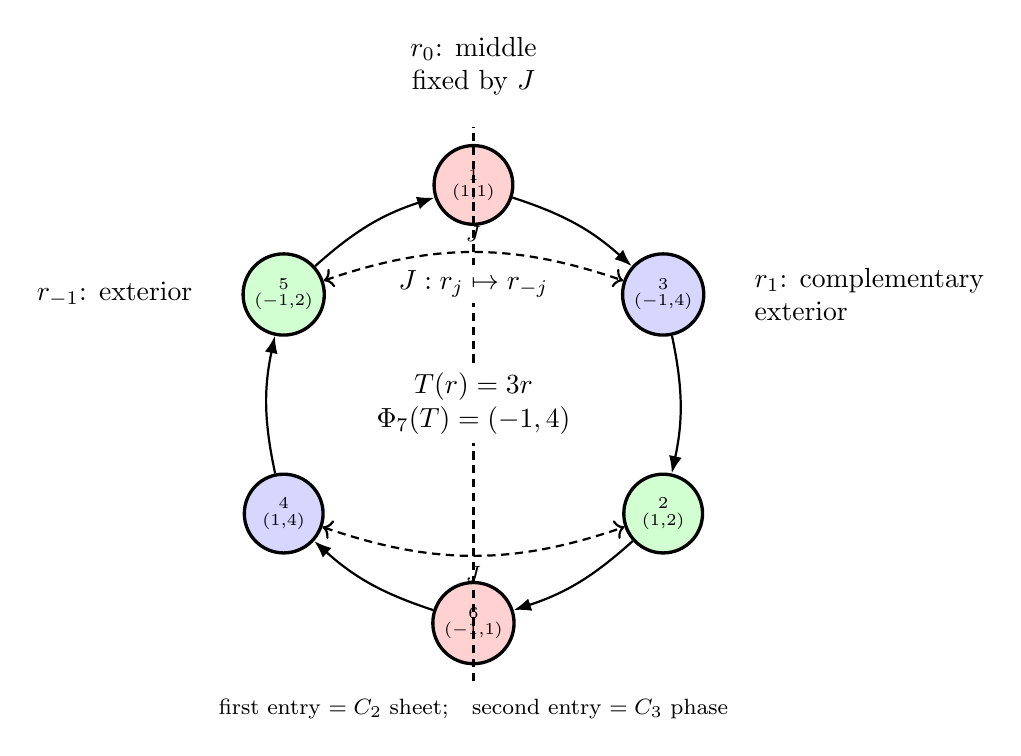
\begin{tikzpicture}[
 scale=1.05,
 orbit/.style={
  circle,
  draw=black,
  very thick,
  minimum size=10mm,
  inner sep=1pt,
  font=\small
 },
 rot/.style={-{Latex[length=2.2mm]},thick},
 refl/.style={<->,densely dashed,thick}
]
 \node[orbit,fill=red!18]   (r0) at (90:2.65)
  {\(\begin{smallmatrix}1\\(1,1)\end{smallmatrix}\)};
 \node[orbit,fill=blue!16]  (r1) at (30:2.65)
  {\(\begin{smallmatrix}3\\(-1,4)\end{smallmatrix}\)};
 \node[orbit,fill=green!18] (r2) at (-30:2.65)
  {\(\begin{smallmatrix}2\\(1,2)\end{smallmatrix}\)};
 \node[orbit,fill=red!18]   (r3) at (-90:2.65)
  {\(\begin{smallmatrix}6\\(-1,1)\end{smallmatrix}\)};
 \node[orbit,fill=blue!16]  (r4) at (-150:2.65)
  {\(\begin{smallmatrix}4\\(1,4)\end{smallmatrix}\)};
 \node[orbit,fill=green!18] (r5) at (150:2.65)
  {\(\begin{smallmatrix}5\\(-1,2)\end{smallmatrix}\)};

 \draw[rot] (r0) to[bend left=12] (r1);
 \draw[rot] (r1) to[bend left=12] (r2);
 \draw[rot] (r2) to[bend left=12] (r3);
 \draw[rot] (r3) to[bend left=12] (r4);
 \draw[rot] (r4) to[bend left=12] (r5);
 \draw[rot] (r5) to[bend left=12] (r0);

 \draw[densely dashed,very thick] (0,-3.35) -- (0,3.35);
 \node[fill=white,inner sep=2pt] at (0,1.45)
  {\(J:r_j\mapsto r_{-j}\)};
 \draw[refl] (r5) to[bend left=19]
  node[above,font=\footnotesize] {\(J\)} (r1);
 \draw[refl] (r4) to[bend right=19]
  node[below,font=\footnotesize] {\(J\)} (r2);

 \node[above=5mm of r0,align=center]
  {\(r_0\): middle\\fixed by \(J\)};
 \node[left=5mm of r5,align=right]
  {\(r_{-1}\): exterior};
 \node[right=5mm of r1,align=left]
  {\(r_1\): complementary\\exterior};
 \node[fill=white,inner sep=2pt] at (0,0)
  {\(\begin{gathered}
     T(r)=3r\\[-1mm]
     \Phi_7(T)=(-1,4)
    \end{gathered}\)};
 \node[below=3mm of r3,align=center,font=\footnotesize]
  {first entry \(=C_2\) sheet;\quad second entry \(=C_3\) phase};
\end{tikzpicture}
\caption{The exact endpoint target orbit for \(p=73\), \(R=7\).
Each node displays \(r_j\) above \(\Phi_7(r_j)\).  Multiplication by
\(p\equiv3\) advances the six-cycle, simultaneously flipping the
\(C_2\) sheet and rotating the \(C_3\) phase.  Divisor complement is
the reflection \(J\); it fixes the middle target and exchanges the two
labelled exterior directions.}
\label{fig:R7-p73-endpoint-c6}
\end{figure}

\begin{computation}[Endpoint dihedral-orbit checker]
\label{comp:endpoint-dihedral-orbit-check}
The script and captured receipt
\[
\begin{gathered}
 \texttt{verification/verify\_endpoint\_dihedral\_orbit.py},\\
 \texttt{verification/verify\_endpoint\_dihedral\_orbit\_output.txt}
\end{gathered}
\]
verify the multiplicative target transport, complement reflection,
dihedral relation, and three-fibre rank identity in all \(67810\)
admissible shells through \(p=2000\), comprising \(1666950\) divisors
with multiplicity.  They also verify the complete
\(C_2\)-sheet/\(C_3\)-phase cycle in
\eqref{eq:R7-p73-c2-c3-cycle}.
\end{computation}

\begin{theorem}[Support-orbit classification of the endpoint channels]
\label{thm:endpoint-support-orbit-classification}
Retain the conditions of \cref{thm:endpoint-dihedral-orbit}, and put
\begin{equation}
 S_{R,a}
 :=
 \{r\in U_R:\mathcal F_{R,a}(r)\ne\varnothing\},
 \qquad
 H_{R,a}
 :=
 \{h\in U_R:hS_{R,a}=S_{R,a}\}.
 \label{eq:endpoint-support-and-rotation-stabilizer}
\end{equation}
Then
\begin{equation}
 J_{R,a}(S_{R,a})=S_{R,a},
 \qquad
 H_{R,a}\le U_R.
 \label{eq:endpoint-support-reflection-and-stabilizer}
\end{equation}
The endpoint-channel status is determined exactly by the intersection
of \(S_{R,a}\) with the three labelled targets:
\begin{equation}
\begin{array}{c|c}
 \text{channel status}
 &
 \text{target support}\\ \hline
 \text{empty}
 &
 S_{R,a}\cap\{r_{-1},r_0,r_1\}=\varnothing\\
 \text{exterior only}
 &
 r_{-1},r_1\in S_{R,a},\quad r_0\notin S_{R,a}\\
 \text{middle only}
 &
 r_0\in S_{R,a},\quad r_{-1},r_1\notin S_{R,a}\\
 \text{both}
 &
 r_{-1},r_0,r_1\in S_{R,a}.
\end{array}
\label{eq:endpoint-support-four-patterns}
\end{equation}
In particular,
\begin{equation}
 q_{R,p}>0
 \quad\Longleftrightarrow\quad
 S_{R,a}\cap\{r_{-1},r_0,r_1\}\ne\varnothing.
 \label{eq:endpoint-rank-support-intersection}
\end{equation}

If \(\overline p\in H_{R,a}\), membership in \(S_{R,a}\) is constant
on the complete target orbit
\[
 \mathcal O_{R,p,a}:=\{r_j:j\in\mathbb Z\}.
\]
Hence an exterior-only or middle-only shell necessarily satisfies
\begin{equation}
 \overline p\notin H_{R,a}.
 \label{eq:one-sided-shell-breaks-rotation-stability}
\end{equation}
The reverse implication fails.  At
\((p,R,a)=(73,11,21)\),
\begin{equation}
 S_{11,21}=\{1,3,4,5,7,8,9,10\},
 \qquad
 (r_{-1},r_0,r_1)=(8,1,7),
 \label{eq:R11-p73-support-counterexample}
\end{equation}
so both channels are occupied, while
\(\overline p=\overline7\notin H_{11,21}\) because
\(4\in S_{11,21}\) and \(7\cdot4\equiv6\notin S_{11,21}\pmod{11}\).
\end{theorem}

\begin{proof}
The divisor complement \(u\mapsto a^2/u\) is a bijection of the
divisors of \(a^2\), and its residue action is \(J_{R,a}\).
This proves \(J_{R,a}(S_{R,a})=S_{R,a}\).

The identity fixes \(S_{R,a}\).  If \(h\) and \(k\) fix it, then so
does \(hk\); if \(hS_{R,a}=S_{R,a}\), applying \(h^{-1}\) gives
\(h^{-1}S_{R,a}=S_{R,a}\).  Thus \(H_{R,a}\) is a subgroup.

The exterior and middle fibres are
\(\mathcal F_{R,a}(r_{-1})\) and
\(\mathcal F_{R,a}(r_0)\).  Reflection stability gives
\[
 r_{-1}\in S_{R,a}
 \quad\Longleftrightarrow\quad
 r_1\in S_{R,a}.
\]
This proves the four rows of
\eqref{eq:endpoint-support-four-patterns}; the three-fibre identity
\eqref{eq:endpoint-three-fibre-rank} then proves
\eqref{eq:endpoint-rank-support-intersection}.

If \(\overline p\in H_{R,a}\), then
\(T_{R,p}(S_{R,a})=S_{R,a}\).  Since
\(r_j=T_{R,p}^{\,j}(r_0)\), every point of
\(\mathcal O_{R,p,a}\) has the same membership status.  This proves
\eqref{eq:one-sided-shell-breaks-rotation-stability}.  Finally, the
divisors of \(21^2\), reduced modulo \(11\), give the support set in
\eqref{eq:R11-p73-support-counterexample}; the displayed
multiplication by \(7\) proves the last assertion.
\end{proof}

\begin{computation}[Endpoint-support and rotational-stabilizer audit]
\label{comp:endpoint-support-stabilizer-check}
The script and captured receipt
\[
\begin{gathered}
 \texttt{verification/verify\_endpoint\_support\_stabilizers.py},\\
 \texttt{verification/verify\_endpoint\_support\_stabilizers\_output.txt}
\end{gathered}
\]
verify \cref{thm:endpoint-support-orbit-classification} in all
\(67810\) admissible shells through \(p=2000\), comprising
\(1666950\) divisors with multiplicity.  The exact occupancy counts
are
\[
\begin{array}{c|rrrr}
 \text{status}&\text{empty}&\text{exterior only}&\text{middle only}&\text{both}\\
 \hline
 \text{shells}&65253&1642&314&601.
\end{array}
\]
Among these shells, \(\overline pS_{R,a}=S_{R,a}\) holds in \(316\)
empty cases and \(455\) both-channel cases, and in no one-sided case.
There are \(146\) both-channel shells without this rotational
support-stability, beginning with \((73,11,21)\).
\end{computation}

\begin{theorem}[Complete Boolean endpoint-to-blade cell bridge]
\label{thm:endpoint-Boolean-blade-cell-bridge}
Retain the conditions of
\cref{thm:endpoint-support-orbit-classification}.  Define
\begin{equation}
 b_j:=\mathbf1_{S_{R,a}}(r_j)\in\{0,1\},
 \qquad
 e_1:=e_+,\quad e_0:=e_-,
 \qquad
 J_{\mathrm B}:=e_1e_1^{\mathsf T}-e_0e_0^{\mathsf T}.
 \label{eq:endpoint-Boolean-status-basis}
\end{equation}
The two consecutive directed target edges have Boolean cells
\begin{equation}
 C_{-0}:=e_{b_0}e_{b_{-1}}^{\mathsf T},
 \qquad
 C_{0+}:=e_{b_1}e_{b_0}^{\mathsf T}.
 \label{eq:endpoint-directed-Boolean-cells}
\end{equation}
Then
\begin{equation}
 b_{-1}=b_1,
 \qquad
 C_{0+}=C_{-0}^{\mathsf T},
 \label{eq:endpoint-reflected-Boolean-cells}
\end{equation}
and
\begin{align}
 J_{\mathrm B}C_{-0}
 &=(2b_0-1)C_{-0},
 &
 C_{-0}J_{\mathrm B}
 &=(2b_{-1}-1)C_{-0}.
 \label{eq:endpoint-Boolean-cell-bimodule-signs}
\end{align}

Put
\begin{equation}
 \beta_{R,p}
 :=
 (b_0-b_{-1},\,b_1-b_0).
 \label{eq:endpoint-directed-boundary-vector}
\end{equation}
The four support patterns and both directed Boolean cells are
\begin{equation}
\begin{array}{c|c|c|c|c}
 \text{status}
 & (b_{-1},b_0,b_1)
 & \beta_{R,p}
 & C_{-0}
 & C_{0+}\\ \hline
 \text{empty}
 &(0,0,0)&(0,0)&E_{22}&E_{22}\\
 \text{exterior only}
 &(1,0,1)&(-1,+1)&E_{21}&E_{12}\\
 \text{middle only}
 &(0,1,0)&(+1,-1)&E_{12}&E_{21}\\
 \text{both}
 &(1,1,1)&(0,0)&E_{11}&E_{11}.
\end{array}
\label{eq:endpoint-complete-Boolean-blade-table}
\end{equation}
Under the exact Hadamard intertwiner of
\cref{thm:mixer-projectors-ordered-blade-channels}, the ordered pair
\((C_{-0},C_{0+})\) becomes
\begin{equation}
\begin{array}{c|c}
 \text{status}
 &
 (HC_{-0}H^{\mathsf T},HC_{0+}H^{\mathsf T})\\ \hline
 \text{empty}&(P_-,P_-)\\
 \text{exterior only}&(B_{-+},B_{+-})\\
 \text{middle only}&(B_{+-},B_{-+})\\
 \text{both}&(P_+,P_+).
\end{array}
\label{eq:endpoint-complete-Hadamard-edge-pairs}
\end{equation}
Thus every one-sided pattern contains both ordered off-diagonal masks,
one on each reflected edge; their order distinguishes the two
patterns.  The empty and both-channel patterns give the two diagonal
mixer projectors.  The Boolean cells record the support masks; the
integer fibre populations remain in
\eqref{eq:endpoint-three-fibre-rank}.
\end{theorem}

\begin{proof}
The unique Boolean support character of
\cref{thm:unique-Boolean-support-character} assigns \(1\) to a
supported fibre and \(0\) to an unsupported fibre.  The reflection
stability in
\eqref{eq:endpoint-support-reflection-and-stabilizer} gives
\(b_{-1}=b_1\), and hence
\[
 e_{b_1}e_{b_0}^{\mathsf T}
 =
 \left(e_{b_0}e_{b_{-1}}^{\mathsf T}\right)^{\mathsf T}.
\]
Since
\[
 J_{\mathrm B}e_b=(2b-1)e_b
 \qquad(b\in\{0,1\}),
\]
left and right multiplication prove
\eqref{eq:endpoint-Boolean-cell-bimodule-signs}.

The equality \(b_{-1}=b_1\) leaves the four bit strings displayed in
\eqref{eq:endpoint-complete-Boolean-blade-table}.  Substitution in
\eqref{eq:endpoint-directed-Boolean-cells} gives the four matrix
units on each edge and the four boundary vectors.  Finally,
\cref{thm:mixer-projectors-ordered-blade-channels} gives
\[
 HE_{22}H^{\mathsf T}=P_-,
 \quad
 HE_{21}H^{\mathsf T}=B_{-+},
 \quad
 HE_{12}H^{\mathsf T}=B_{+-},
 \quad
 HE_{11}H^{\mathsf T}=P_+.
\]
Applying these four identities to both transpose-related columns of
\eqref{eq:endpoint-complete-Boolean-blade-table} proves
\eqref{eq:endpoint-complete-Hadamard-edge-pairs}.
\end{proof}

\begin{corollary}[The \(R=107\) shell selects the outgoing blade edge]
\label{cor:R107-outgoing-Boolean-blade-selection}
For the shell
\[
 (p,R,a)=(8803369,107,2200869),
\]
one has
\begin{equation}
 (b_{-1},b_0,b_1)=(0,1,0),
 \qquad
 C_{-0}=E_{12},
 \qquad
 C_{0+}=E_{21},
 \qquad
 q_{107,8803369}=1.
 \label{eq:R107-directed-Boolean-edge-pair}
\end{equation}
Consequently the population lift of the outgoing edge is
\begin{equation}
 2q_{107,8803369}C_{0+}
 =
 2E_{21}
 =
 \mathcal M(53).
 \label{eq:R107-outgoing-edge-is-observed-blade}
\end{equation}
The incoming edge is the transposed mask \(E_{12}\), whose coefficient
at residue \(53\) is zero.  Hence the exact coefficient calculation
selects the outgoing direction \(r_0\to r_1\).
\end{corollary}

\begin{proof}
\Cref{comp:first-residual-107-coefficient-only-shell} gives
\(\mathcal E_{107,2200869}=\varnothing\),
\(|\mathcal M_{107,2200869}|=2\), and \(q_{107,8803369}=1\).
The middle-only row of
\eqref{eq:endpoint-complete-Boolean-blade-table} gives the two cells.
The directed coefficient and the absence of its transpose are
\eqref{eq:directed-blade-target}.
\end{proof}

\begin{computation}[Boolean endpoint-to-blade certificate]
\label{comp:endpoint-Boolean-blade-certificate}
The script and captured receipt
\[
\begin{gathered}
 \texttt{verification/verify\_endpoint\_Boolean\_blade\_bridge.py},\\
 \texttt{verification/verify\_endpoint\_Boolean\_blade\_bridge\_output.txt}
\end{gathered}
\]
verify the reflection transpose, both bimodule signs, source and range
projectors, boundary vectors, all eight directed Hadamard images, and
the \(R=107\) outgoing-edge selection over \(\mathbb Q(\sqrt2)\).
\end{computation}

\begin{theorem}[Support-boundary involution and discrete blade commutator]
\label{thm:endpoint-support-boundary-commutator}
Retain the conditions and notation of
\cref{thm:endpoint-support-orbit-classification}.  Write \(T=T_{R,p}\),
\(J=J_{R,a}\), and \(S=S_{R,a}\), and define the outgoing and incoming
boundary-source sets
\begin{equation}
 \partial_T^{\mathrm{out}}S
 :=
 S\setminus T^{-1}(S),
 \qquad
 \partial_T^{\mathrm{in}}S
 :=
 T^{-1}(S)\setminus S.
 \label{eq:endpoint-support-directed-boundaries}
\end{equation}
The crossed reflection
\begin{equation}
 K:=J\circ T
 \label{eq:endpoint-crossed-reflection}
\end{equation}
is an involution and restricts to mutually inverse bijections
\begin{equation}
 \partial_T^{\mathrm{out}}S
 \xleftrightarrow[\ K\ ]{\ K\ }
 \partial_T^{\mathrm{in}}S.
 \label{eq:endpoint-boundary-crossed-reflection-bijection}
\end{equation}

For \(r\in U_R\), put
\begin{equation}
 b(r):=\mathbf1_S(r),
 \qquad
 C_T(r):=e_{b(Tr)}e_{b(r)}^{\mathsf T},
 \qquad
 \nabla_Tb(r):=b(Tr)-b(r).
 \label{eq:endpoint-discrete-support-cell}
\end{equation}
Then the four transitions are
\begin{equation}
\begin{array}{c|c|c|c}
 b(r)\longrightarrow b(Tr)
 &\nabla_Tb(r)
 &C_T(r)
 &\text{boundary status}\\ \hline
 0\longrightarrow0&0&E_{22}&\text{neither}\\
 0\longrightarrow1&+1&E_{12}&r\in\partial_T^{\mathrm{in}}S\\
 1\longrightarrow0&-1&E_{21}&r\in\partial_T^{\mathrm{out}}S\\
 1\longrightarrow1&0&E_{11}&\text{neither}.
\end{array}
\label{eq:endpoint-four-boundary-cells}
\end{equation}
Their exact commutator is
\begin{equation}
 [J_{\mathrm B},C_T(r)]
 =
 2\nabla_Tb(r)\,C_T(r).
 \label{eq:endpoint-discrete-boundary-commutator}
\end{equation}
For
\begin{equation}
 D:=3I_2+6J_{\mathrm B}
   =\operatorname{diag}(9,-3),
 \label{eq:endpoint-boundary-modular-matrix}
\end{equation}
one consequently has
\begin{equation}
 [D,C_T(r)]
 =
 12\nabla_Tb(r)\,C_T(r).
 \label{eq:endpoint-boundary-twelve-commutator}
\end{equation}
Thus \(E_{12}\) is the \(+12\) entry-boundary line and \(E_{21}\) is
the \(-12\) exit-boundary line.

On the two labelled endpoint edges, exterior-only support gives
\begin{equation}
 r_{-1}\in\partial_T^{\mathrm{out}}S,
 \qquad
 r_0\in\partial_T^{\mathrm{in}}S,
 \qquad
 (C_{-0},C_{0+})=(E_{21},E_{12}),
 \label{eq:exterior-only-exit-entry-order}
\end{equation}
whereas middle-only support gives
\begin{equation}
 r_{-1}\in\partial_T^{\mathrm{in}}S,
 \qquad
 r_0\in\partial_T^{\mathrm{out}}S,
 \qquad
 (C_{-0},C_{0+})=(E_{12},E_{21}).
 \label{eq:middle-only-entry-exit-order}
\end{equation}
In particular, the \(R=107\) coefficient satisfies
\begin{equation}
 \mathcal M(53)
 =
 2q_{107,8803369}C_T(r_0)
 =
 2E_{21},
 \qquad
 r_0\in\partial_T^{\mathrm{out}}S_{107,2200869}.
 \label{eq:R107-blade-is-exit-boundary}
\end{equation}
\end{theorem}

\begin{proof}
The dihedral relation \(J\circ T\circ J=T^{-1}\) gives
\[
 K^2=J\circ T\circ J\circ T=I.
\]
If \(r\in\partial_T^{\mathrm{out}}S\), then \(r\in S\) and
\(Tr\notin S\).  Since \(J(S)=S\), one has \(J(Tr)\notin S\), while
\[
 T(J(Tr))=Jr\in S
\]
because \(T\circ J\circ T=J\).  Hence \(Kr=J(Tr)\) lies in
\(\partial_T^{\mathrm{in}}S\).  Applying the involution \(K\) again proves
\eqref{eq:endpoint-boundary-crossed-reflection-bijection}.

The four possibilities for \((b(r),b(Tr))\) give
\eqref{eq:endpoint-four-boundary-cells} directly from
\(C_T(r)=e_{b(Tr)}e_{b(r)}^{\mathsf T}\).  Left and right multiplication
by \(J_{\mathrm B}\) give
\[
 J_{\mathrm B}C_T(r)
 =(2b(Tr)-1)C_T(r),
 \qquad
 C_T(r)J_{\mathrm B}
 =(2b(r)-1)C_T(r).
\]
Their difference is
\eqref{eq:endpoint-discrete-boundary-commutator}.  Since scalar matrices
have zero commutator,
\[
 [D,C_T(r)]
 =
 6[J_{\mathrm B},C_T(r)],
\]
which proves \eqref{eq:endpoint-boundary-twelve-commutator}.

The exterior-only support word \(101\) gives an exit on
\(r_{-1}\to r_0\) and an entry on \(r_0\to r_1\).  The middle-only word
\(010\) reverses those two transitions.  This proves
\eqref{eq:exterior-only-exit-entry-order} and
\eqref{eq:middle-only-entry-exit-order}.  Finally,
\cref{cor:R107-outgoing-Boolean-blade-selection} gives the middle-only
word, \(q_{107,8803369}=1\), and
\(\mathcal M(53)=2C_{0+}=2E_{21}\), proving
\eqref{eq:R107-blade-is-exit-boundary}.
\end{proof}

\begin{computation}[Endpoint-boundary and commutator replay]
\label{comp:endpoint-boundary-commutator-replay}
The script and captured receipt
\[
\begin{gathered}
 \texttt{verification/verify\_endpoint\_boundary\_commutator.py},\\
 \texttt{verification/verify\_endpoint\_boundary\_commutator\_output.txt}
\end{gathered}
\]
verify the crossed-reflection boundary bijection in all \(67810\)
admissible shells through \(p=2000\).  The scan finds \(1419667\)
outgoing boundary sources and the same number of incoming boundary
sources.  On the \(135620\) labelled endpoint edges, the transition
counts are
\[
\begin{array}{c|rrrr}
\text{transition}&0\to0&0\to1&1\to0&1\to1\\ \hline
\text{count}&130506&1956&1956&1202.
\end{array}
\]
The checker also verifies both commutator identities for all four Boolean
cells and replays the \(R=107\) exit-boundary coefficient.  Its total
support-boundary energy is \(2839334\); exactly \(771\) scanned shells
have zero energy, and the labelled endpoint energy is \(3912\).
\end{computation}

\begin{corollary}[Support-boundary Dirichlet energy and Lorentz sum]
\label{cor:endpoint-support-boundary-Dirichlet-energy}
Retain the conditions and notation of
\cref{thm:endpoint-support-boundary-commutator}.  Define
\begin{equation}
 \mathscr E^\partial_{R,p}
 :=
 \frac14
 \sum_{r\in U_R}
 \bigl\lVert[J_{\mathrm B},C_T(r)]\bigr\rVert_{\mathrm{HS}}^2.
 \label{eq:endpoint-support-boundary-energy}
\end{equation}
Then
\begin{equation}
 \boxed{
 \begin{aligned}
 \mathscr E^\partial_{R,p}
 &=
 \frac1{144}
 \sum_{r\in U_R}
 \bigl\lVert[D,C_T(r)]\bigr\rVert_{\mathrm{HS}}^2\\
 &=
 \sum_{r\in U_R}\bigl(\nabla_Tb(r)\bigr)^2\\
 &=
 \bigl|S\mathbin{\triangle}T^{-1}(S)\bigr|\\
 &=
 2\bigl|\partial_T^{\mathrm{out}}S\bigr|
 =
 2\bigl|\partial_T^{\mathrm{in}}S\bigr|.
 \end{aligned}}
 \label{eq:endpoint-support-boundary-energy-identities}
\end{equation}
In particular, \(\mathscr E^\partial_{R,p}\) is a nonnegative even integer,
and
\begin{equation}
 \mathscr E^\partial_{R,p}=0
 \quad\Longleftrightarrow\quad
 T(S)=S
 \quad\Longleftrightarrow\quad
 \overline p\in H_{R,a}.
 \label{eq:endpoint-zero-energy-stabilizer}
\end{equation}

For each \(r\in U_R\), put
\begin{equation}
 \mathfrak H_T(r)
 :=
 C_T(r)^{\mathsf T}C_T(r)
 -
 e_{b(Tr)}e_{b(Tr)}^{\mathsf T},
 \qquad
 \mathcal N_T(r):=-\det\mathfrak H_T(r).
 \label{eq:endpoint-unit-cell-Lorentz-carrier}
\end{equation}
Then
\begin{equation}
 \mathcal N_T(r)
 =
 \bigl(\nabla_Tb(r)\bigr)^2,
 \qquad
 \mathscr E^\partial_{R,p}
 =
 \sum_{r\in U_R}\mathcal N_T(r).
 \label{eq:endpoint-support-boundary-Lorentz-sum}
\end{equation}
Thus the complete finite Dirichlet energy is the sum of the Lorentz norms
of the unit-mass endpoint cells.

The two labelled edges have energy
\begin{equation}
 \begin{aligned}
 \mathscr E^{\mathrm{lab}}_{R,p}
 &:=
 \frac14\left(
  \bigl\lVert[J_{\mathrm B},C_{-0}]\bigr\rVert_{\mathrm{HS}}^2
  +
  \bigl\lVert[J_{\mathrm B},C_{0+}]\bigr\rVert_{\mathrm{HS}}^2
 \right)\\
 &=
 (b_0-b_{-1})^2+(b_1-b_0)^2
 =
 2(b_0-b_{-1})^2.
 \end{aligned}
 \label{eq:endpoint-labelled-boundary-energy}
\end{equation}
Consequently,
\begin{equation}
 \mathscr E^{\mathrm{lab}}_{R,p}
 =
 \begin{cases}
 2,&\text{for an exterior-only or middle-only shell},\\
 0,&\text{for an empty or both-channel shell}.
 \end{cases}
 \label{eq:endpoint-labelled-energy-classification}
\end{equation}
For the first occupied \(R=107\) shell,
\begin{equation}
 \mathscr E^\partial_{107,8803369}=20,
 \qquad
 \mathscr E^{\mathrm{lab}}_{107,8803369}=2.
 \label{eq:R107-support-boundary-energies}
\end{equation}
\end{corollary}

\begin{proof}
The commutator formulas in
\cref{thm:endpoint-support-boundary-commutator} and the unit
Hilbert--Schmidt norm of every matrix unit give
\[
 \frac14
 \bigl\lVert[J_{\mathrm B},C_T(r)]\bigr\rVert_{\mathrm{HS}}^2
 =
 \frac1{144}
 \bigl\lVert[D,C_T(r)]\bigr\rVert_{\mathrm{HS}}^2
 =
 \bigl(\nabla_Tb(r)\bigr)^2.
\]
The last quantity equals one exactly when membership of \(r\) in \(S\)
differs from membership of \(r\) in \(T^{-1}(S)\).  Summation therefore
gives the symmetric-difference formula in
\eqref{eq:endpoint-support-boundary-energy-identities}.  The symmetric
difference is the disjoint union of the outgoing and incoming
boundary-source sets.  Their cardinalities agree by
\eqref{eq:endpoint-boundary-crossed-reflection-bijection}, proving the
remaining equalities.

The energy vanishes exactly when \(T^{-1}(S)=S\), equivalently
\(T(S)=S\).  The definition of \(H_{R,a}\) in
\eqref{eq:endpoint-support-and-rotation-stabilizer} gives
\eqref{eq:endpoint-zero-energy-stabilizer}.

Equation \eqref{eq:endpoint-unit-cell-Lorentz-carrier} is the
unit-mass case of the directed Gram--support carrier in
\eqref{eq:four-cell-directed-carrier}.  The four rows of
\eqref{eq:four-cell-exact-Lorentz-table} give
\(\mathcal N_T(r)=0\) on stationary cells and
\(\mathcal N_T(r)=1\) on entry or exit cells.  This proves
\eqref{eq:endpoint-support-boundary-Lorentz-sum}.

Finally, \(b_{-1}=b_1\) by
\eqref{eq:endpoint-reflected-Boolean-cells}.  Substitution into the
two-edge commutator sum proves
\eqref{eq:endpoint-labelled-boundary-energy}.  The four support words in
\eqref{eq:endpoint-complete-Boolean-blade-table} give
\eqref{eq:endpoint-labelled-energy-classification}.  The exact \(R=107\)
values are replayed by
\cref{comp:endpoint-boundary-commutator-replay}.
\end{proof}

\begin{theorem}[Coupled-shell three-orbit balance]
\label{thm:coupled-shell-three-orbit-balance}
Let \(p\equiv1\pmod4\) be prime, let \(a\in\mathscr A_p\), and put
\(R=4a-p\).  For every squarefree coordinate
\[
 a=stm,
 \qquad
 s\ \text{squarefree},
\]
one has
\begin{equation}
 \left(
 R\mid4st^2+1
 \ \text{and}\
 R\mid t+m
 \right)
 \quad\Longrightarrow\quad
 R\mid p-1.
 \label{eq:shared-coordinate-forces-coupling}
\end{equation}
If \(R\mid p-1\), then for every such coordinate,
\begin{equation}
 R\mid4st^2+1
 \quad\Longleftrightarrow\quad
 R\mid t+m.
 \label{eq:coupled-channel-equivalence}
\end{equation}

Suppose \(R\mid p-1\), and define
\begin{equation}
 \mathcal T_{R,a}
 :=
 \left\{
 (s,\{t,m\}):
 \begin{array}{c}
 s,t,m\in\mathbb Z_{>0},\ s\ \text{squarefree},\\
 a=stm,\ R\mid4st^2+1
 \end{array}
 \right\}.
 \label{eq:coupled-shell-packet-set}
\end{equation}
The exterior condition in
\eqref{eq:coupled-shell-packet-set} is invariant under
\(t\leftrightarrow m\).  Every packet contributes exactly the three
distinct complement orbits
\begin{align}
 \{(2,st^2),(0,sm^2)\},
 \qquad
 \{(2,sm^2),(0,st^2)\},
 \qquad
 \{(1,st^2),(1,sm^2)\}.
 \label{eq:coupled-shell-three-orbit-packet}
\end{align}
These are all occupied orbits in the shell.  Hence
\begin{equation}
 q_{R,p}=3|\mathcal T_{R,a}|.
 \label{eq:coupled-shell-three-orbit-count}
\end{equation}
In particular,
\begin{align}
 Q_p
 &\ge3|\mathcal T_{R,a}|,
 \label{eq:coupled-shell-primewise-rank-bound}\\
 \operatorname{Vol}^{\det}_p
 &\ge2^{18|\mathcal T_{R,a}|},
 \label{eq:coupled-shell-volume-bound}\\
 L_{H,p}^2
 &\ge153|\mathcal T_{R,a}|,
 \qquad
 L_{K,p}^2
 \ge\frac{225}{2}|\mathcal T_{R,a}|.
 \label{eq:coupled-shell-length-bounds}
\end{align}

The coupled shells for \(p\) are indexed exactly by
\begin{equation}
 \{R:R\mid p-1,\ R\equiv3\pmod4\}.
 \label{eq:coupled-shell-divisor-index}
\end{equation}
\end{theorem}

\begin{proof}
Suppose both coordinate congruences in
\eqref{eq:shared-coordinate-forces-coupling} hold.  Then
\[
 m\equiv-t\pmod R,
\]
so
\[
 a=stm\equiv-st^2\pmod R.
\]
The exterior congruence now gives
\[
 p=4a-R
 \equiv-4st^2
 \equiv1
 \pmod R,
\]
proving \eqref{eq:shared-coordinate-forces-coupling}.

Now suppose \(R\mid p-1\).  Since \(p=4a-R\),
\begin{equation}
 4a\equiv1\pmod R.
 \label{eq:coupled-shell-four-a}
\end{equation}
If \(R\mid4st^2+1\), then
\[
 (-t)(4st)\equiv1\pmod R.
\]
On the other hand, \(a=stm\) and
\eqref{eq:coupled-shell-four-a} give
\[
 m(4st)\equiv1\pmod R.
\]
Because \(\gcd(R,4st)=1\), these two inverse expressions imply
\[
 m\equiv-t\pmod R.
\]
Thus \(R\mid t+m\).  Conversely, if \(R\mid t+m\), then
\[
 4a=4stm\equiv-4st^2\pmod R.
\]
Equation \eqref{eq:coupled-shell-four-a} yields
\(R\mid4st^2+1\), proving
\eqref{eq:coupled-channel-equivalence}.

The equivalence is unchanged by exchanging \(t\) and \(m\), so the
exterior coordinate set is complement-stable.  A fixed point
\(t=m\) would give \(R\mid2t\); this is impossible because
\(\gcd(R,t)=1\) and \(R\ge3\).  Each packet therefore has two ordered
exterior coordinates and one unordered middle coordinate.
\Cref{thm:squarefree-two-channel-shell-coordinates} identifies these
with the three orbits in
\eqref{eq:coupled-shell-three-orbit-packet} and proves
\eqref{eq:coupled-shell-three-orbit-count}.  The quantitative bounds
follow from
\cref{cor:squarefree-coordinate-complexity-volume}.

Finally, a coupled shell necessarily has \(R\mid p-1\) and
\(R\equiv3\pmod4\).  Conversely, if \(R\) is a positive divisor of
\(p-1\) with \(R\equiv3\pmod4\), then
\[
 a=\frac{p+R}{4}
\]
is an integer satisfying
\[
 \frac p4<a<\frac p2<\frac{3p}{4}.
\]
Thus \(a\in\mathscr A_p\) and \(4a-p=R\), proving
\eqref{eq:coupled-shell-divisor-index}.
\end{proof}

\begin{corollary}[Coupled-shell equality of divisor support sections]
\label{cor:coupled-shell-divisor-section-equality}
Retain the conditions of
\cref{thm:coupled-shell-three-orbit-balance}, and assume
\(R\mid p-1\).  Then the complete exterior and middle divisor sets
coincide:
\begin{equation}
 \boxed{
 \mathcal E_{R,a}
 =
 \mathcal M_{R,a}
 =
 \left\{
  u\in\mathbb Z_{>0}:
  u\mid a^2,\
  u\equiv-a\equiv-\overline4^{-1}\pmod R
 \right\}.}
 \label{eq:coupled-shell-divisor-section-equality}
\end{equation}
Consequently,
\begin{equation}
 q_{R,p}
 =
 \frac32|\mathcal E_{R,a}|
 =
 \frac32|\mathcal M_{R,a}|,
 \qquad
 q_{R,p}>0
 \quad\Longleftrightarrow\quad
 \mathcal E_{R,a}=\mathcal M_{R,a}\ne\varnothing.
 \label{eq:coupled-shell-common-section-rank}
\end{equation}
The complement involution \(u\mapsto a^2/u\) acts without fixed
points on this common section, so its cardinality is even.
\end{corollary}

\begin{proof}
The coupling condition and \(p=4a-R\) give
\[
 4a\equiv p\equiv1\pmod R,
 \qquad
 a\equiv\overline4^{-1}\pmod R.
\]
For every \(u\mid a^2\),
\[
 R\mid4u+1
 \quad\Longleftrightarrow\quad
 u\equiv-\overline4^{-1}
 \quad\Longleftrightarrow\quad
 u\equiv-a
 \quad\Longleftrightarrow\quad
 R\mid u+a.
\]
The definitions
\eqref{eq:complete-endpoint-exterior-divisors} and
\eqref{eq:complete-endpoint-middle-divisors} now prove
\eqref{eq:coupled-shell-divisor-section-equality}.  Substitution in
\eqref{eq:complete-endpoint-orbit-count} proves
\eqref{eq:coupled-shell-common-section-rank}.  The final assertion is
the fixed-point-free middle complement theorem in
\cref{cor:complete-endpoint-coordinate-divisor-count}.
\end{proof}

\begin{corollary}[First failure of universal coupled-shell coverage]
\label{cor:first-coupled-shell-coverage-failure}
For \(p=73\), every coupled shell is empty, whereas the noncoupled
shell \(R=7\) has rank \(4\).
\end{corollary}

\begin{proof}
The divisors of \(p-1=72\) that are \(3\pmod4\) consist only of
\(R=3\).  Its denominator is
\[
 a=\frac{73+3}{4}=19,
\]
and
\[
 \{u:u\mid19^2\}=\{1,19,361\}
 \equiv\{1\}\pmod3.
\]
Both endpoint targets equal
\(-a\equiv-4^{-1}\equiv2\pmod3\).  Hence
\begin{equation}
 \mathcal E_{3,19}
 =
 \mathcal M_{3,19}
 =
 \varnothing.
 \label{eq:p73-coupled-empty}
\end{equation}

For \(R=7\),
\[
 a=\frac{73+7}{4}=20,
 \qquad
 \delta_{7,73}
 =
 4^{-1}-20
 \equiv3\pmod7.
\]
Direct divisor evaluation gives
\begin{equation}
 \mathcal E_{7,20}=\{5,40\},
 \qquad
 \mathcal M_{7,20}=\{1,8,50,400\}.
 \label{eq:p73-noncoupled-sections}
\end{equation}
The exterior target \(5\pmod7\) is carried by the displacement \(3\)
to the middle target \(1\pmod7\), exactly as in
\cref{thm:endpoint-divisor-fibre-displacement}.  Therefore
\[
 q_{7,73}
 =
 |\mathcal E_{7,20}|
 +
 \frac12|\mathcal M_{7,20}|
 =
 2+2
 =
 4.
\]
Since \(7\nmid72\), this occupied shell lies outside the coupled
family.
\end{proof}

\begin{computation}[Finite coupled-shell coverage and displacement scan]
\label{comp:coupled-shell-coverage-scan}
The script and captured receipt
\[
\begin{gathered}
 \texttt{verification/scan\_coupled\_shell\_coverage.py},\\
 \texttt{verification/scan\_coupled\_shell\_coverage\_output.txt}
\end{gathered}
\]
enumerate every prime \(p\le10^6\) with \(p\equiv1\pmod{12}\), every
coupled residual \(R\mid p-1\) with \(R\equiv3\pmod4\), and every
divisor of the associated \(a^2\).  Among the \(19564\) relevant
primes, \(16757\) have an occupied coupled shell and \(2807\) have
none.  Every one of those \(2807\) primes has an occupied general
shell with first residual at most \(59\).  At that first general
shell, \(2750\) primes meet both endpoint fibres, \(36\) meet only the
exterior fibre, and \(21\) meet only the middle fibre.  The receipt
records the complete residual distributions and the first witnesses
in each one-sided class.
\end{computation}

\begin{computation}[Coupled-shell three-orbit checker]
\label{comp:coupled-shell-three-orbit-check}
The script and captured receipt
\[
\begin{gathered}
 \texttt{verification/verify\_coupled\_shell\_three\_orbit\_balance.py},\\
 \texttt{verification/verify\_coupled\_shell\_three\_orbit\_balance\_output.txt}
\end{gathered}
\]
verify the forcing implication, the channel equivalence, literal
equality of the complete divisor sections, complement stability, and
the three-orbit count for every admissible shell through \(p=5000\).
The replay checks the divisor-set equality in all \(625\) coupled
shells in that range.
\end{computation}

\begin{theorem}[All-shell unit-group coefficient and modular rank]
\label{thm:all-shell-unit-group-modular-rank}
Let \(p\equiv1\pmod4\) be prime, let \(a\in\mathscr A_p\), put
\(R=4a-p\), and factor
\[
 a=\prod_{\ell^e\parallel a}\ell^e.
\]
Retain the divisor sets \(\mathcal E_{R,a}\) and
\(\mathcal M_{R,a}\) from
\eqref{eq:complete-endpoint-exterior-divisors} and
\eqref{eq:complete-endpoint-middle-divisors}.
Let
\[
 U_R=(\mathbb Z/R\mathbb Z)^\times
\]
and write \([\overline v]\) for the basis element of
\(\mathbb Z[U_R]\) indexed by the residue of a unit \(v\).  Define
\begin{equation}
 \mathfrak P_{R,a}
 :=
 \prod_{\ell^e\parallel a}
 \left(
 [\overline1]
 +
 \sum_{j=1}^{e}
 \bigl(
 [\overline{\ell}^{\,j}]
 +
 [\overline{\ell}^{\,-j}]
 \bigr)
 \right)
 \in\mathbb Z[U_R]
 \label{eq:coupled-shell-unit-group-element}
\end{equation}
and let
\[
 c_{R,a}
 :=
 \operatorname{coeff}_{[\overline{-1}]}
 \mathfrak P_{R,a}.
\]
Then
\begin{equation}
 \boxed{
 c_{R,a}=|\mathcal M_{R,a}|,}
 \qquad
 c_{R,a}\equiv0\pmod2,
 \label{eq:all-shell-unit-group-middle-count}
\end{equation}
and
\begin{equation}
 \boxed{
 q_{R,p}
 =
 |\mathcal E_{R,a}|+\frac12c_{R,a}
 =
 \operatorname{rank}P^{\mathrm{mod}}_{R,p}.}
 \label{eq:all-shell-unit-group-modular-rank}
\end{equation}
When \(q_{R,p}>0\), the exact shell complexity quantities are
\begin{align}
 \operatorname{Vol}^{\det}_{R,p}
 &=
 2^{\,6|\mathcal E_{R,a}|+3c_{R,a}},
 \label{eq:all-shell-unit-group-volume}\\
 L_H^2
 &=
 51|\mathcal E_{R,a}|+\frac{51}{2}c_{R,a},
 \label{eq:all-shell-unit-group-H-length}\\
 L_K^2
 &=
 \frac{75}{2}|\mathcal E_{R,a}|
 +\frac{75}{4}c_{R,a}.
 \label{eq:all-shell-unit-group-K-length}
\end{align}

Finite Fourier inversion on \(U_R\) gives
\begin{equation}
 c_{R,a}
 =
 \frac1{\varphi(R)}
 \sum_{\chi\in\widehat U_R}
 \chi(-1)
 \prod_{\ell^e\parallel a}
 \left(
 1+
 \sum_{j=1}^{e}
 \bigl(
 \chi(\ell)^j+\chi(\ell)^{-j}
 \bigr)
 \right).
 \label{eq:coupled-shell-character-rank}
\end{equation}
\end{theorem}

\begin{proof}
The identities \(0<a<p\) and \(R=4a-p\) give
\(\gcd(R,a)=1\).  Thus every divisor of \(a\) represents a unit
modulo \(R\).

Consider the ordered coprime-factor set
\[
 \widetilde{\mathcal C}_{R,a}
 =
 \{(x,y):x,y>0,\ \gcd(x,y)=1,\ xy\mid a,\ R\mid x+y\}.
\]
At a prime power \(\ell^e\parallel a\), an ordered pair in this set
chooses one of
\[
 \ell\nmid xy,
 \qquad
 \ell^j\parallel x\quad(1\le j\le e),
 \qquad
 \ell^j\parallel y\quad(1\le j\le e).
\]
These three types contribute
\[
 \overline1,
 \qquad
 \overline\ell^{\,j},
 \qquad
 \overline\ell^{\,-j}
\]
to the unit ratio
\(\overline x\,\overline y^{\,-1}\).  Expansion of
\eqref{eq:coupled-shell-unit-group-element} therefore gives
\[
 c_{R,a}
 =
 \#\{(x,y):x,y>0,\ \gcd(x,y)=1,\ xy\mid a,\
 \overline x\,\overline y^{\,-1}=\overline{-1}\}.
\]
Since \(y\) is a unit modulo \(R\), the final equality is equivalent
to \(R\mid x+y\).  Hence
\[
 c_{R,a}=|\widetilde{\mathcal C}_{R,a}|.
\]

The exchange \((x,y)\mapsto(y,x)\) is free: a fixed point would have
\(x=y=1\), contrary to \(R\mid2\) for the odd integer \(R\ge3\).
It follows that
\[
 c_{R,a}=2|\mathcal C_{R,a}|.
\]
The bijection
\eqref{eq:middle-coprime-factor-bijection} identifies
\(\mathcal C_{R,a}\) with the complement orbits in
\(\mathcal M_{R,a}\).  The complement action on
\(\mathcal M_{R,a}\) is free by
\cref{cor:complete-endpoint-coordinate-divisor-count}.  Therefore
\[
 c_{R,a}
 =
 2|\mathcal C_{R,a}|
 =
 |\mathcal M_{R,a}|,
\]
which proves \eqref{eq:all-shell-unit-group-middle-count}.

Equation \eqref{eq:complete-endpoint-orbit-count} now gives the first
equality in \eqref{eq:all-shell-unit-group-modular-rank}, and
\eqref{eq:shellwise-modular-support-rank-nullity} gives the second.
Substitution in
\eqref{eq:general-shell-determinant-volume},
\eqref{eq:general-shell-HS-length}, and
\eqref{eq:general-shell-traceless-length} proves
\eqref{eq:all-shell-unit-group-volume}--%
\eqref{eq:all-shell-unit-group-K-length}.

Finally, evaluate \(\mathfrak P_{R,a}\) under each character of
\(U_R\) and apply finite Fourier inversion.  The element
\(\overline{-1}\) has order two, so
\(\overline{\chi(-1)}=\chi(-1)\), which proves
\eqref{eq:coupled-shell-character-rank}.
\end{proof}

\begin{theorem}[Finite factor-residue support ideal]
\label{thm:finite-factor-residue-support-ideal}
Retain the conditions of
\cref{thm:all-shell-unit-group-modular-rank}.  For
\(g\in U_R\setminus\{\overline1\}\), define
\[
 \nu_g(a)
 :=
 \sum_{\substack{\ell^e\parallel a\\
                 \overline\ell=g}}e
\]
and write
\[
 \boldsymbol\nu_R(a)
 =
 \bigl(\nu_g(a)\bigr)_{g\ne\overline1}.
\]
For an arbitrary vector
\(\boldsymbol\nu\in
\mathbb Z_{\ge0}^{\,U_R\setminus\{\overline1\}}\), put
\begin{align}
 \mathscr R_R^{\mathrm E}(\boldsymbol\nu)
 &:=
 \left\{
 \prod_{g\ne\overline1}g^{e_g}:
 0\le e_g\le2\nu_g
 \right\},
 \label{eq:general-residual-exterior-reachability}\\
 \mathscr R_R^{\mathrm M}(\boldsymbol\nu)
 &:=
 \left\{
 \prod_{g\ne\overline1}g^{d_g}:
 -\nu_g\le d_g\le\nu_g
 \right\}.
 \label{eq:general-residual-middle-reachability}
\end{align}
Let
\[
 t_R:=\overline{-4^{-1}}\in U_R,
 \qquad
 s_R:=\overline{-1}\in U_R,
\]
and define the occupied valuation up-set
\[
 \mathscr U_R
 :=
 \left\{
 \boldsymbol\nu:
 t_R\in\mathscr R_R^{\mathrm E}(\boldsymbol\nu)
 \ \text{or}\
 s_R\in\mathscr R_R^{\mathrm M}(\boldsymbol\nu)
 \right\}.
\]
Its coordinatewise-minimal subset
\[
 \operatorname{Min}(\mathscr U_R)
\]
is finite.  In the polynomial ring with variables
\(\{X_g:g\in U_R\setminus\{\overline1\}\}\), define
\begin{equation}
 I_R
 :=
 \left\langle
 \prod_{g\ne\overline1}X_g^{\mu_g}:
 \boldsymbol\mu\in\operatorname{Min}(\mathscr U_R)
 \right\rangle
 \label{eq:general-residual-support-ideal}
\end{equation}
and
\[
 \mathfrak m_R(a)
 :=
 \prod_{g\ne\overline1}X_g^{\nu_g(a)}.
\]
Then
\begin{equation}
 \boxed{
 q_{R,p}>0
 \quad\Longleftrightarrow\quad
 \mathfrak m_R(a)\in I_R.}
 \label{eq:general-residual-ideal-membership}
\end{equation}

Let \(D(U_R)\) denote the least positive integer such that every
sequence of \(D(U_R)\) elements of \(U_R\) contains a nonempty
subsequence with product \(\overline1\).  Every minimal generator of
\(I_R\) has total degree at most
\begin{equation}
 D(U_R)-1.
 \label{eq:general-residual-support-ideal-degree}
\end{equation}
\end{theorem}

\begin{proof}
A divisor \(u\mid a^2\) chooses, for every residue class \(g\), an
exponent between \(0\) and \(2\nu_g(a)\).  Hence
\[
 \mathcal E_{R,a}\ne\varnothing
 \quad\Longleftrightarrow\quad
 t_R\in
 \mathscr R_R^{\mathrm E}\bigl(\boldsymbol\nu_R(a)\bigr).
\]
For the middle channel, collect all prime powers of \(a\) having the
same residue \(g\).  Their local exponent intervals add to the full
integer interval
\([-\nu_g(a),\nu_g(a)]\).  Expansion of
\eqref{eq:coupled-shell-unit-group-element} therefore gives
\[
 c_{R,a}>0
 \quad\Longleftrightarrow\quad
 s_R\in
 \mathscr R_R^{\mathrm M}\bigl(\boldsymbol\nu_R(a)\bigr).
\]
Factors congruent to \(1\pmod R\) may change positive multiplicities,
but they do not change either support set.

The set \(\mathscr U_R\) is closed under coordinatewise increase.
Consequently,
\[
 \boldsymbol\nu_R(a)\in\mathscr U_R
 \quad\Longleftrightarrow\quad
 \boldsymbol\nu_R(a)
 \text{ dominates an element of }
 \operatorname{Min}(\mathscr U_R),
\]
which is equivalent to
\(\mathfrak m_R(a)\in I_R\).
Equation
\eqref{eq:all-shell-unit-group-modular-rank} now proves
\eqref{eq:general-residual-ideal-membership}.

It remains to prove finiteness and the degree bound.  Suppose first that
\(t_R\) has a representation in
\(\mathscr R_R^{\mathrm E}(\boldsymbol\nu)\).  Write this representation
as a sequence containing \(e_g\) copies of \(g\).  Whenever its length
is at least \(D(U_R)\), remove a nonempty product-one subsequence.
Iteration leaves a representation of \(t_R\) of length at most
\(D(U_R)-1\).  If \(e'_g\) is the remaining multiplicity, then
\[
 \mu_g:=\left\lceil\frac{e'_g}{2}\right\rceil
\]
defines an occupied vector dominated by \(\boldsymbol\nu\), and
\[
 \sum_g\mu_g
 \le
 \sum_g e'_g
 \le
 D(U_R)-1.
\]

For a middle representation, use \(|d_g|\) labelled copies of \(g\)
or \(g^{-1}\), according to the sign of \(d_g\).  The same subsequence
removal leaves a target representation of length at most
\(D(U_R)-1\).  Its remaining absolute multiplicities define an
occupied vector dominated by \(\boldsymbol\nu\) and of total degree at
most \(D(U_R)-1\).  Thus every occupied vector dominates one in the
finite box
\[
 \left\{
 \boldsymbol\mu:
 \sum_g\mu_g\le D(U_R)-1
 \right\}.
\]
All coordinatewise-minimal occupied vectors lie in this box, proving
finiteness and
\eqref{eq:general-residual-support-ideal-degree}.
\end{proof}

\begin{theorem}[Safe-residual parity-sheet reduction]
\label{thm:safe-residual-parity-sheet-reduction}
Retain the conditions of
\cref{thm:finite-factor-residue-support-ideal}.  Suppose
\[
 R=2q+1
\]
with \(q\) an odd prime.  Choose a primitive root
\(\gamma\in U_R\), and let
\[
 \lambda_R:U_R\longrightarrow\mathbb Z/(2q)\mathbb Z,
 \qquad
 \lambda_R(\gamma)=1
\]
be the corresponding additive logarithm.  Put
\[
 r_R:=\lambda_R(\overline2).
\]
Write the prime factorization of \(a\), with each prime repeated
according to its valuation, as
\[
 a=\ell_1\cdots\ell_m,
 \qquad
 \kappa_i:=\lambda_R(\overline{\ell_i}).
\]
Indices with \(\kappa_i=0\) may be omitted.  Define
\begin{align}
 \mathscr B_R^{\mathrm M}(\boldsymbol\kappa)
 &:=
 \left\{
  \sum_{i=1}^m\delta_i\kappa_i:
  \delta_i\in\{-1,0,1\}
 \right\},
 \label{eq:safe-residual-middle-occurrence-box}\\
 \mathscr B_R^{\mathrm E}(\boldsymbol\kappa)
 &:=
 \left\{
  \sum_{i=1}^m\epsilon_i\kappa_i:
  \epsilon_i\in\{0,1,2\}
 \right\}
 \label{eq:safe-residual-exterior-occurrence-box}
\end{align}
in \(\mathbb Z/(2q)\mathbb Z\).  Then
\begin{equation}
 \lambda_R(s_R)=q,
 \qquad
 \lambda_R(t_R)=q-2r_R,
 \label{eq:safe-residual-two-odd-targets}
\end{equation}
and
\begin{equation}
 q_{R,p}>0
 \quad\Longleftrightarrow\quad
 q\in\mathscr B_R^{\mathrm M}(\boldsymbol\kappa)
 \ \text{or}\
 q-2r_R\in\mathscr B_R^{\mathrm E}(\boldsymbol\kappa).
 \label{eq:safe-residual-two-box-criterion}
\end{equation}

Both targets in
\eqref{eq:safe-residual-two-odd-targets} are odd.  Consequently, every
middle representation satisfies
\begin{equation}
 \#\{i:\kappa_i\ \text{is odd and }\delta_i\ne0\}
 \equiv1\pmod2,
 \label{eq:safe-residual-middle-odd-occurrence-parity}
\end{equation}
and every exterior representation satisfies
\begin{equation}
 \#\{i:\kappa_i\ \text{is odd and }\epsilon_i=1\}
 \equiv1\pmod2.
 \label{eq:safe-residual-exterior-odd-occurrence-parity}
\end{equation}
In particular, if every nonzero factor logarithm of \(a\) is even,
then \(q_{R,p}=0\).

Suppose now that exactly one factor-logarithm occurrence is odd; denote
it by \(k\).  Write every remaining occurrence as
\(\kappa_i=2h_i\) in \(\mathbb Z/(2q)\mathbb Z\), and define
\begin{align}
 \mathscr A_R^{\mathrm M}
 &:=
 \left\{
  \sum_i\delta_i h_i:
  \delta_i\in\{-1,0,1\}
 \right\},
 \label{eq:safe-residual-reduced-middle-box}\\
 \mathscr A_R^{\mathrm E}
 &:=
 \left\{
  \sum_i\epsilon_i h_i:
  \epsilon_i\in\{0,1,2\}
 \right\}
 \label{eq:safe-residual-reduced-exterior-box}
\end{align}
in \(\mathbb Z/q\mathbb Z\).  The complete occupation criterion is
\begin{equation}
 \boxed{
 q_{R,p}>0
 \quad\Longleftrightarrow\quad
 \frac{q-k}{2}\in\mathscr A_R^{\mathrm M}
 \ \text{or}\
 \frac{q+k}{2}\in\mathscr A_R^{\mathrm M}
 \ \text{or}\
 \frac{q-2r_R-k}{2}\in\mathscr A_R^{\mathrm E}.}
 \label{eq:safe-residual-one-odd-quotient-criterion}
\end{equation}
Each displayed half is the class modulo \(q\) of the indicated even
integer divided by \(2\).
\end{theorem}

\begin{proof}
Since \(\gamma\) has order \(2q\),
\[
 \lambda_R(\overline{-1})=q.
\]
Moreover,
\[
 \lambda_R(\overline{-4^{-1}})
 =
 \lambda_R(\overline{-1})-\lambda_R(\overline4)
 =
 q-2r_R,
\]
which proves \eqref{eq:safe-residual-two-odd-targets}.  Repeating each
prime factor according to its valuation converts the intervals in
\eqref{eq:general-residual-exterior-reachability} and
\eqref{eq:general-residual-middle-reachability} into independent
occurrence coefficients \(\epsilon_i\in\{0,1,2\}\) and
\(\delta_i\in\{-1,0,1\}\), respectively.  Applying \(\lambda_R\) to
\cref{thm:finite-factor-residue-support-ideal} proves
\eqref{eq:safe-residual-two-box-criterion}.

Reduction modulo \(2\) proves
\eqref{eq:safe-residual-middle-odd-occurrence-parity} and
\eqref{eq:safe-residual-exterior-odd-occurrence-parity}.  If all
\(\kappa_i\) are even, neither odd target can occur.

Assume that \(k\) is the unique odd occurrence.  In the middle channel
its coefficient must be \(1\) or \(-1\).  Subtracting \(k\), or adding
\(k\), and then dividing the resulting congruence by \(2\) gives the
first two membership tests in
\eqref{eq:safe-residual-one-odd-quotient-criterion}.  In the exterior
channel the coefficient of \(k\) must be \(1\).  Subtracting \(k\) and
dividing by \(2\) gives the third membership test.  These steps are
reversible, proving the equivalence.
\end{proof}

\begin{corollary}[Canonical Legendre-sheet form]
\label{cor:safe-residual-Legendre-sheet-form}
Under the conditions of
\cref{thm:safe-residual-parity-sheet-reduction}, let
\[
 Q_R:=\{u^2:u\in U_R\}
\]
be the quadratic-residue subgroup and let
\(\chi_R:U_R\to\{\pm1\}\) be the quadratic character.  The map
\begin{equation}
 \Phi_R:U_R\longrightarrow\{\pm1\}\times Q_R,
 \qquad
 \Phi_R(u)=\bigl(\chi_R(u),\chi_R(u)u\bigr)
 \label{eq:safe-residual-canonical-sheet-map}
\end{equation}
is a group isomorphism.  Its target values are
\begin{equation}
 \Phi_R(s_R)=(-1,1),
 \qquad
 \Phi_R(t_R)=(-1,\overline4^{-1}).
 \label{eq:safe-residual-canonical-target-pair}
\end{equation}

For each repeated factor occurrence, write
\[
 \Phi_R(\overline{\ell_i})=(\sigma_i,v_i).
\]
Then the shell is occupied exactly when at least one of the following
two systems has a solution:
\begin{align}
 \prod_i\sigma_i^{\delta_i}&=-1,
 &
 \prod_i v_i^{\delta_i}&=1,
 &
 \delta_i&\in\{-1,0,1\},
 \label{eq:safe-residual-canonical-middle-system}\\
 \prod_i\sigma_i^{\epsilon_i}&=-1,
 &
 \prod_i v_i^{\epsilon_i}&=\overline4^{-1},
 &
 \epsilon_i&\in\{0,1,2\}.
 \label{eq:safe-residual-canonical-exterior-system}
\end{align}
If exactly one occurrence, indexed by \(0\), is a quadratic
nonresidue, then \(v_0=-\overline{\ell_0}\in Q_R\) and the criterion
becomes
\begin{equation}
 \begin{aligned}
 q_{R,p}>0
 \quad\Longleftrightarrow\quad&
 v_0^{-1}\in
 \left\{\prod_{i\ne0}v_i^{\delta_i}:
       \delta_i\in\{-1,0,1\}\right\}\\
 &\text{or}\quad
 v_0\in
 \left\{\prod_{i\ne0}v_i^{\delta_i}:
       \delta_i\in\{-1,0,1\}\right\}\\
 &\text{or}\quad
 \overline4^{-1}v_0^{-1}\in
 \left\{\prod_{i\ne0}v_i^{\epsilon_i}:
       \epsilon_i\in\{0,1,2\}\right\}.
 \end{aligned}
 \label{eq:safe-residual-canonical-one-nonresidue-criterion}
\end{equation}

For \(R=7\),
\[
 Q_7=\{\overline1,\overline2,\overline4\}
     =\langle\overline2\rangle\cong C_3,
\]
and
\begin{equation}
 U_7\cong C_2\times C_3,
 \qquad
 s_7\longmapsto(-1,\overline1),
 \qquad
 t_7\longmapsto(-1,\overline2).
 \label{eq:R7-exact-C2-C3-target-carrier}
\end{equation}
Thus the \(R=7\) shell has an exact binary sheet and three-phase
carrier; the Boolean coordinate
\[
 \operatorname{Supp}_{7,p}(a)
 :=\mathbf1_{\{q_{7,p}>0\}}
\]
records whether either distinguished point on the nonresidue sheet is
reached.
\end{corollary}

\begin{proof}
Because \(q\) is odd, \(R\equiv3\pmod4\), so
\(\chi_R(-1)=-1\).  Hence
\(\chi_R(u)u\in Q_R\) for every \(u\in U_R\), and
\eqref{eq:safe-residual-canonical-sheet-map} is a homomorphism.  Its
inverse is
\[
 (\sigma,v)\longmapsto\sigma v.
\]
This proves the isomorphism.  Since \(4^{-1}\) is a square,
\eqref{eq:safe-residual-canonical-target-pair} follows immediately.
Applying \(\Phi_R\) to the two occurrence boxes in
\eqref{eq:safe-residual-two-box-criterion} gives
\eqref{eq:safe-residual-canonical-middle-system} and
\eqref{eq:safe-residual-canonical-exterior-system}.

With one nonresidue occurrence, the sheet equations force
\(\delta_0=1\) or \(-1\) in the middle channel and
\(\epsilon_0=1\) in the exterior channel.  Solving the corresponding
\(Q_R\)-equations proves
\eqref{eq:safe-residual-canonical-one-nonresidue-criterion}.  Finally,
\(Q_7=\langle\overline2\rangle\), while
\[
 s_7=\overline6,
 \qquad
 t_7=\overline5,
 \qquad
 -\overline5=\overline2.
\]
This proves \eqref{eq:R7-exact-C2-C3-target-carrier}.
\end{proof}

\begin{corollary}[The \(R=107\) carrier has exactly two parity sheets]
\label{cor:R107-exact-parity-sheets}
Retain the notation of
\cref{thm:champion-divisor-tag-orbit}.  For \(R_\ast=107\),
\[
 q=53,\qquad \gamma=2,\qquad r_{107}=1,
\]
and the factor logarithms of
\[
 a_\ast=3^2\,11^2\,43\,47
\]
are
\[
 70,70,22,22,59,66.
\]
The unique odd occurrence is \(k=59\), arising from \(43\), and the
multiset of even half-logarithms is
\[
 (35,35,11,11,33).
\]
The three reduced targets in
\eqref{eq:safe-residual-one-odd-quotient-criterion} are
\begin{equation}
 \frac{53-59}{2}=50,\qquad
 \frac{53+59}{2}=3,\qquad
 \frac{53-2-59}{2}=49
 \quad\text{in }\mathbb Z/53\mathbb Z.
 \label{eq:R107-three-reduced-parity-targets}
\end{equation}
In the aggregate coefficient box
\[
 -2\le\beta_3,\beta_{11}\le2,
 \qquad
 -1\le\beta_{47}\le1,
\]
the first two target fibres are
\begin{align}
 \{(\beta_3,\beta_{11},\beta_{47}):
   35\beta_3+11\beta_{11}+33\beta_{47}=50\}
 &=\{(2,0,1)\},
 \label{eq:R107-reduced-positive-sheet}\\
 \{(\beta_3,\beta_{11},\beta_{47}):
   35\beta_3+11\beta_{11}+33\beta_{47}=3\}
 &=\{(-2,0,-1)\},
 \label{eq:R107-reduced-negative-sheet}
\end{align}
where the equations are in \(\mathbb Z/53\mathbb Z\).  In the exterior
coefficient box
\[
 0\le\epsilon_3,\epsilon_{11}\le4,
 \qquad
 0\le\epsilon_{47}\le2,
\]
the target \(49\) has no representative.  Hence the two centered
middle vectors and the exterior fibre are exactly
\[
 \beta^-=(-2,0,-1,-1),\qquad
 \beta^+=(2,0,1,1),\qquad
 \mathcal E_{107,a_\ast}=\varnothing.
\]
Furthermore,
\[
 \lambda_{107}(a_\ast)=97,
 \qquad
 \lambda_{107}(t_{107})=51,
 \qquad
 51-97=60\pmod{106}.
 \label{eq:R107-unshifted-to-centered-exterior-target}
\]
Thus \(51\) is the unshifted exterior target and \(60\) is its centered
coordinate in
\cref{thm:champion-divisor-tag-orbit}.  Under the exact blade
identification
\[
 2C_{0+}=2E_{21}=\mathcal M(53),
\]
the two summands are precisely the two parity sheets distinguished by
the coefficient \(+1\) or \(-1\) on the unique odd factor logarithm.
Here \(r_0\in\partial_T^{\mathrm{out}}S_{107,a_\ast}\), so this is the
exit-boundary cell by
\cref{thm:endpoint-support-boundary-commutator}.
The incoming cell is \(C_{-0}=E_{12}\) and has zero coefficient at
residue \(53\), as proved in
\cref{cor:R107-outgoing-Boolean-blade-selection}.
\end{corollary}

\begin{proof}
The logarithms and the two centered fibres were proved in
\cref{thm:champion-divisor-tag-orbit}.  Applying
\cref{thm:safe-residual-parity-sheet-reduction} gives
\eqref{eq:R107-three-reduced-parity-targets}.  The finite table in the
proof of \cref{thm:champion-divisor-tag-orbit} gives the unique
memberships
\eqref{eq:R107-reduced-positive-sheet} and
\eqref{eq:R107-reduced-negative-sheet} and excludes \(49\) from the
exterior box.  Finally,
\[
 2(70)+2(22)+59+66=309\equiv97\pmod{106},
\]
which proves
\eqref{eq:R107-unshifted-to-centered-exterior-target}.  The blade
statement is then
\eqref{eq:champion-divisor-orbit-to-blade-matrix}.
\end{proof}

\begin{computation}[Safe-residual parity replay]
\label{comp:safe-residual-parity-replay}
The script and captured receipt
\[
\begin{gathered}
 \texttt{verification/verify\_safe\_residual\_parity\_bridge.py},\\
 \texttt{verification/verify\_safe\_residual\_parity\_bridge\_output.txt}
\end{gathered}
\]
check the canonical Legendre-sheet isomorphism and both target images
for all \(24\) safe residual primes through \(1000\), verify the exact
\(C_2\times C_3\) target carrier at \(R=7\), compare the full
\(2q\)-modulus boxes with the quotient criterion on \(255837\)
one-odd profiles through \(R=107\), and replay the complete \(R=107\)
calculation.  The latter check returns the
reduced targets
\[
 (50,3,49),
\]
the two centered vectors
\[
 (-2,0,-1,-1),\qquad(2,0,1,1),
\]
an empty exterior fibre, and the target transport
\[
 51-97=60\pmod{106}.
\]
\end{computation}

\begin{corollary}[Consecutive factor-ideal formulation]
\label{cor:consecutive-factor-ideal-formulation}
Let \(p=4n+1\) be prime.  For
\[
 1\le j\le2n,
 \qquad
 a_j:=n+j,
 \qquad
 R_j:=4j-1,
\]
one has
\[
 a_j\in\mathscr A_p,
 \qquad
 4a_j-p=R_j.
\]
Moreover,
\begin{equation}
 \boxed{
 \mathrm{ES}(p)
 \quad\Longleftrightarrow\quad
 \exists\,j\in\{1,\ldots,2n\}:
 \mathfrak m_{R_j}(n+j)\in I_{R_j}.}
 \label{eq:consecutive-factor-ideal-ES}
\end{equation}
Thus a counterexample at \(p\) is exactly a length-\(2n\) affine
sequence satisfying
\begin{equation}
 \mathfrak m_{4j-1}(n+j)\notin I_{4j-1}
 \qquad(1\le j\le2n).
 \label{eq:consecutive-factor-ideal-counterexample}
\end{equation}
\end{corollary}

\begin{proof}
From \(p=4n+1\) and
\eqref{eq:primewise-finite-denominator-set},
\[
 \mathscr A_p=\{n+1,n+2,\ldots,3n\}.
\]
Writing \(a=n+j\) gives \(1\le j\le2n\) and
\[
 R_a=4(n+j)-(4n+1)=4j-1.
\]
The primewise divisor criterion
\eqref{eq:complete-primewise-divisor-criterion}, together with
\cref{thm:finite-factor-residue-support-ideal}, proves
\eqref{eq:consecutive-factor-ideal-ES}.  Negation gives
\eqref{eq:consecutive-factor-ideal-counterexample}.
\end{proof}

\begin{theorem}[Prime-factor colon reduction]
\label{thm:prime-factor-colon-reduction}
Retain the conditions of
\cref{cor:consecutive-factor-ideal-formulation}.  Fix
\(1\le j\le2n\), and write
\[
 R=4j-1,
 \qquad
 a=n+j.
\]
Let \(\ell\) be a prime divisor of \(a\), let
\(1\le e\le v_\ell(a)\), and suppose that the class
\(\overline\ell\in U_R\) is not \(\overline1\).  Then
\begin{equation}
 \mathfrak m_R(a)
 =
 X_{\overline\ell}^{\,e}
 \mathfrak m_R\!\left(\frac{a}{\ell^e}\right),
 \label{eq:prime-factor-monomial-extraction}
\end{equation}
and
\begin{equation}
 \boxed{
 q_{R,p}>0
 \quad\Longleftrightarrow\quad
 \mathfrak m_R\!\left(\frac{a}{\ell^e}\right)
 \in
 (I_R:X_{\overline\ell}^{\,e}).}
 \label{eq:prime-factor-colon-reduction}
\end{equation}
\end{theorem}

\begin{proof}
The factor-residue valuation of \(a/\ell^e\) is obtained from that of
\(a\) by subtracting \(e\) in the
\(\overline\ell\)-coordinate.  This proves
\eqref{eq:prime-factor-monomial-extraction}.  For every monomial \(M\),
\[
 X_{\overline\ell}^{\,e}M\in I_R
 \quad\Longleftrightarrow\quad
 M\in(I_R:X_{\overline\ell}^{\,e}).
\]
Apply this identity to
\eqref{eq:prime-factor-monomial-extraction} and use
\eqref{eq:general-residual-ideal-membership}.
\end{proof}

\begin{theorem}[Three-position target packets after factor extraction]
\label{thm:three-position-target-packets}
Retain the conditions of
\cref{thm:prime-factor-colon-reduction} with \(e=1\), and write
\(a=\ell b\).  Define two subsets of \(U_R\):
\begin{align}
 \mathcal T_{R,\ell}^{\mathrm E}
 &:=
 \left\{
 t_R,\,
 t_R\overline\ell^{\,-1},\,
 t_R\overline\ell^{\,-2}
 \right\},
 \label{eq:exterior-three-position-target-packet}\\
 \mathcal T_{R,\ell}^{\mathrm M}
 &:=
 \left\{
 s_R\overline\ell,\,
 s_R,\,
 s_R\overline\ell^{\,-1}
 \right\}.
 \label{eq:middle-three-position-target-packet}
\end{align}
Then
\begin{equation}
 \boxed{
 q_{R,p}>0
 \quad\Longleftrightarrow\quad
 \mathscr R_R^{\mathrm E}\bigl(\boldsymbol\nu_R(b)\bigr)
 \cap\mathcal T_{R,\ell}^{\mathrm E}\ne\varnothing
 \quad\text{or}\quad
 \mathscr R_R^{\mathrm M}\bigl(\boldsymbol\nu_R(b)\bigr)
 \cap\mathcal T_{R,\ell}^{\mathrm M}\ne\varnothing.}
 \label{eq:three-position-target-packet-criterion}
\end{equation}
\end{theorem}

\begin{proof}
The extracted prime factor \(\ell\) may occur in an exterior divisor
with local exponent \(0,1,\) or \(2\).  Hence
\[
 \mathscr R_R^{\mathrm E}\bigl(\boldsymbol\nu_R(a)\bigr)
 =
 \bigcup_{j=0}^{2}
 \overline\ell^{\,j}
 \mathscr R_R^{\mathrm E}\bigl(\boldsymbol\nu_R(b)\bigr).
\]
The exterior target \(t_R\) belongs to this union exactly when the
reduced reachability set meets
\(\mathcal T_{R,\ell}^{\mathrm E}\).

In the middle channel the extracted factor has local signed exponent
\(-1,0,\) or \(1\), so
\[
 \mathscr R_R^{\mathrm M}\bigl(\boldsymbol\nu_R(a)\bigr)
 =
 \bigcup_{d=-1}^{1}
 \overline\ell^{\,d}
 \mathscr R_R^{\mathrm M}\bigl(\boldsymbol\nu_R(b)\bigr).
\]
Solving \(s_R=\overline\ell^{\,d}u\) for the reduced target \(u\)
gives \(\mathcal T_{R,\ell}^{\mathrm M}\).  The general reachability
criterion in
\cref{thm:finite-factor-residue-support-ideal} proves
\eqref{eq:three-position-target-packet-criterion}.
\end{proof}

\begin{corollary}[Exact homothety between the two extracted-factor packets]
\label{cor:extracted-factor-packet-homothety}
Under the conditions of
\cref{thm:three-position-target-packets}, put
\[
 \alpha_{R,\ell}:=(4\overline\ell)^{-1}\in U_R.
\]
Then
\begin{equation}
 \boxed{
 \mathcal T_{R,\ell}^{\mathrm E}
 =
 \alpha_{R,\ell}\,
 \mathcal T_{R,\ell}^{\mathrm M}.}
 \label{eq:extracted-factor-packet-homothety}
\end{equation}
Thus the exterior and middle packets are two scalar-related ordered
length-three orbit segments.  This statement uses no order-three action.
\end{corollary}

\begin{proof}
Put
\[
 \mathcal B_{R,\ell}
 :=
 \{1,\overline\ell^{-1},\overline\ell^{-2}\}.
\]
Since \(t_R=-4^{-1}\) and \(s_R=-1\), the definitions give
\[
 \mathcal T_{R,\ell}^{\mathrm E}
 =t_R\mathcal B_{R,\ell},
 \qquad
 \mathcal T_{R,\ell}^{\mathrm M}
 =s_R\overline\ell\,\mathcal B_{R,\ell}.
\]
Their scalar ratio is
\[
 \frac{t_R}{s_R\overline\ell}
 =
 \frac{-4^{-1}}{-\overline\ell}
 =
 (4\overline\ell)^{-1}.
\]
This proves \eqref{eq:extracted-factor-packet-homothety}.
\end{proof}

\begin{theorem}[Weighted packet exchange and ordered-blade amplitude ratio]
\label{thm:weighted-packet-exchange-ordered-blade-ratio}
Retain the conditions of
\cref{cor:extracted-factor-packet-homothety}, set
\[
 A_R:=\mathbb Z/R\mathbb Z,
 \qquad
 \alpha:=\alpha_{R,\ell},
\]
and form the ordered packet-channel module
\[
 V_{R,\ell}
 :=
 A_R e_{\mathrm E}\oplus A_R e_{\mathrm M}.
\]
The map
\begin{equation}
 \mathscr J_{R,\ell}
 \begin{pmatrix}x\\y\end{pmatrix}
 :=
 \begin{pmatrix}0&\alpha\\ \alpha^{-1}&0\end{pmatrix}
 \begin{pmatrix}x\\y\end{pmatrix}
 \label{eq:weighted-packet-exchange-matrix}
\end{equation}
is an involution and exchanges the two tagged packets:
\begin{align}
 \mathscr J_{R,\ell}
 \bigl(\mathcal T_{R,\ell}^{\mathrm E}e_{\mathrm E}\bigr)
 &=
 \mathcal T_{R,\ell}^{\mathrm M}e_{\mathrm M},
 \notag\\
 \mathscr J_{R,\ell}
 \bigl(\mathcal T_{R,\ell}^{\mathrm M}e_{\mathrm M}\bigr)
 &=
 \mathcal T_{R,\ell}^{\mathrm E}e_{\mathrm E}.
 \label{eq:weighted-packet-exchange-tagged-packets}
\end{align}

Let
\[
 W_R:=A_RE_{21}\oplus A_RE_{12}\subset M_2(A_R),
 \qquad
 S:=E_{12}+E_{21},
\]
and let \(\mathscr S(X):=SXS\).  Every line-preserving
\(A_R\)-module isomorphism
\[
 \Phi:V_{R,\ell}\longrightarrow W_R
\]
that satisfies
\[
 \Phi\mathscr J_{R,\ell}=\mathscr S\Phi
\]
has the form
\begin{equation}
 \Phi_u(e_{\mathrm E})=uE_{21},
 \qquad
 \Phi_u(e_{\mathrm M})=\alpha uE_{12}
 \qquad
 (u\in U_R).
 \label{eq:packet-to-ordered-blade-intertwiner}
\end{equation}
Consequently an equal-amplitude carriage,
\[
 \Phi(e_{\mathrm E})=uE_{21},
 \qquad
 \Phi(e_{\mathrm M})=uE_{12},
\]
exists if and only if \(\alpha=1\).

Finally, define the packet and blade gradings by
\[
 \Gamma_{\mathrm P}e_{\mathrm E}=-e_{\mathrm E},
 \qquad
 \Gamma_{\mathrm P}e_{\mathrm M}=e_{\mathrm M},
\]
\[
 \Gamma_{\mathrm B}E_{21}=-E_{21},
 \qquad
 \Gamma_{\mathrm B}E_{12}=E_{12}.
\]
Then
\begin{equation}
 \Phi_u\Gamma_{\mathrm P}=\Gamma_{\mathrm B}\Phi_u,
 \qquad
 \mathscr J_{R,\ell}\Gamma_{\mathrm P}
 =-\Gamma_{\mathrm P}\mathscr J_{R,\ell},
 \qquad
 \mathscr S\Gamma_{\mathrm B}
 =-\Gamma_{\mathrm B}\mathscr S.
 \label{eq:packet-blade-graded-intertwining}
\end{equation}
The blade grading is the sign grading of the two modular channels in
\cref{thm:N2-Fourier-blade-channels}.
\end{theorem}

\begin{proof}
The matrix in
\eqref{eq:weighted-packet-exchange-matrix} has square \(I_2\).
Equation \eqref{eq:extracted-factor-packet-homothety} gives
\[
 \alpha^{-1}\mathcal T_{R,\ell}^{\mathrm E}
 =\mathcal T_{R,\ell}^{\mathrm M},
 \qquad
 \alpha\mathcal T_{R,\ell}^{\mathrm M}
 =\mathcal T_{R,\ell}^{\mathrm E},
\]
which proves
\eqref{eq:weighted-packet-exchange-tagged-packets}.

Write
\[
 \Phi(e_{\mathrm E})=u_{\mathrm E}E_{21},
 \qquad
 \Phi(e_{\mathrm M})=u_{\mathrm M}E_{12},
\]
where both coefficients are units.  Since
\[
 \mathscr S(E_{21})=E_{12},
 \qquad
 \mathscr S(E_{12})=E_{21},
\]
the intertwining equation evaluated at \(e_{\mathrm E}\) is
\[
 \alpha^{-1}u_{\mathrm M}E_{12}
 =
 u_{\mathrm E}E_{12}.
\]
Equivalently,
\[
 u_{\mathrm M}=\alpha u_{\mathrm E}.
\]
The equation at \(e_{\mathrm M}\) gives the same condition.  This proves
\eqref{eq:packet-to-ordered-blade-intertwiner} and its converse.  The two
amplitudes are equal exactly when \(\alpha=1\).  The grading identities
follow on the two displayed bases.
\end{proof}

\begin{corollary}[The first two weighted packet--blade carriages]
\label{cor:first-two-weighted-packet-blade-carriages}
For the universal extracted factor \(3\), the first two exchange
matrices and blade amplitude ratios are
\begin{align}
 R=11:\quad&
 [\mathscr J_{11,3}]
 =
 \begin{pmatrix}0&1\\1&0\end{pmatrix},
 &
 \Phi_u(e_{\mathrm E})&=uE_{21},
 &
 \Phi_u(e_{\mathrm M})&=uE_{12},
 \label{eq:R11-unweighted-packet-blade-carriage}\\
 R=23:\quad&
 [\mathscr J_{23,3}]
 =
 \begin{pmatrix}0&2\\12&0\end{pmatrix},
 &
 \Phi_u(e_{\mathrm E})&=uE_{21},
 &
 \Phi_u(e_{\mathrm M})&=2uE_{12}.
 \label{eq:R23-weighted-packet-blade-carriage}
\end{align}
Thus residual \(11\) has an equal-amplitude ordered-blade carriage,
whereas residual \(23\) retains the factor \(2\) between its two ordered
channel lines.
\end{corollary}

\begin{proof}
Modulo \(11\), \(12^{-1}=1\).  Modulo \(23\), \(12^{-1}=2\) and
\(2^{-1}=12\).  Substitute these values into
\eqref{eq:weighted-packet-exchange-matrix} and
\eqref{eq:packet-to-ordered-blade-intertwiner}.
\end{proof}

\begin{theorem}[One-box form of the two divisor channels]
\label{thm:one-box-two-divisor-channels}
Retain the conditions of
\cref{thm:three-position-target-packets}, write \(a=\ell b\), and let
\(\overline b\in U_R\) be the residue class of \(b\).  Then
\begin{equation}
 \boxed{
 \mathscr R_R^{\mathrm E}\bigl(\boldsymbol\nu_R(b)\bigr)
 =
 \overline b\,
 \mathscr R_R^{\mathrm M}\bigl(\boldsymbol\nu_R(b)\bigr).}
 \label{eq:exterior-middle-reachability-homothety}
\end{equation}
Consequently the two-channel packet test is the single signed-box test
\begin{align}
 q_{R,p}>0
 \quad\Longleftrightarrow\quad&
 \mathscr R_R^{\mathrm M}\bigl(\boldsymbol\nu_R(b)\bigr)
 \cap
 \left(
 \mathcal T_{R,\ell}^{\mathrm M}
 \cup
 \overline b^{-1}\mathcal T_{R,\ell}^{\mathrm E}
 \right)
 \ne\varnothing
 \notag\\
 \quad\Longleftrightarrow\quad&
 \mathscr R_R^{\mathrm M}\bigl(\boldsymbol\nu_R(b)\bigr)
 \cap
 \left(
 \mathcal T_{R,\ell}^{\mathrm M}
 \cup
 (4\overline\ell\,\overline b)^{-1}
 \mathcal T_{R,\ell}^{\mathrm M}
 \right)
 \ne\varnothing.
 \label{eq:one-signed-box-double-packet-criterion}
\end{align}
\end{theorem}

\begin{proof}
Write
\[
 \boldsymbol\nu_R(b)=(\nu_g)_{g\in U_R\setminus\{\overline1\}}.
\]
The residue of \(b\) is
\[
 \overline b=\prod_g g^{\nu_g}.
\]
For each exterior exponent \(e_g\) with
\(0\le e_g\le2\nu_g\), put \(d_g=e_g-\nu_g\).  This gives a bijection
\[
 \prod_g\{0,\ldots,2\nu_g\}
 \longleftrightarrow
 \prod_g\{-\nu_g,\ldots,\nu_g\},
\]
and
\[
 \prod_g g^{e_g}
 =
 \overline b\prod_g g^{d_g}.
\]
This proves
\eqref{eq:exterior-middle-reachability-homothety}.  Pulling the exterior
target packet back through multiplication by \(\overline b\) gives the
first line of
\eqref{eq:one-signed-box-double-packet-criterion}.  Equation
\eqref{eq:extracted-factor-packet-homothety} gives the second.
\end{proof}

\begin{theorem}[Universal every-second-shell binary packet]
\label{thm:universal-every-second-shell-binary-packet}
Let \(p=12k+1\) be prime, and let
\(\eta_k\in\{0,1\}\) be determined by
\(\eta_k\equiv k\pmod2\).  For \(1\le m\le3k\), put
\begin{equation}
\begin{split}
 j_m^{(2)}&:=2m-\eta_k,\\
 R_m^{(2)}&:=8m-4\eta_k-1,\\
 b_m^{(2)}&:=\frac{3k-\eta_k}{2}+m.
\end{split}
\label{eq:universal-every-second-shell-coordinates}
\end{equation}
Then
\[
 1\le j_m^{(2)}\le6k,
 \qquad
 3k+j_m^{(2)}=2b_m^{(2)},
 \qquad
 R_m^{(2)}=4j_m^{(2)}-1,
\]
and
\begin{equation}
 8b_m^{(2)}=p+R_m^{(2)}.
 \label{eq:universal-every-second-shell-affine-relation}
\end{equation}
Define
\[
 \mathcal T_m^{(2)}
 :=
 \mathcal T_{R_m^{(2)},2}^{\mathrm M}
 =
 \{-2,-1,-2^{-1}\}
 \subset U_{R_m^{(2)}},
\]
\[
 \mathcal D_{m,p}^{(2)}
 :=
 \mathcal T_m^{(2)}
 \cup
 \overline p^{-1}\mathcal T_m^{(2)}.
\]
Then
\begin{equation}
 \boxed{
 q_{R_m^{(2)},p}>0
 \quad\Longleftrightarrow\quad
 \mathscr R_{R_m^{(2)}}^{\mathrm M}
 \bigl(\boldsymbol\nu_{R_m^{(2)}}(b_m^{(2)})\bigr)
 \cap\mathcal D_{m,p}^{(2)}\ne\varnothing.}
 \label{eq:universal-every-second-shell-one-box-test}
\end{equation}

The only members of this residual family for which \(2\) has order
less than five are \(R=3,7,15\).  Their target volumes are
\begin{align}
 R=3:\quad&
 |\mathcal D_{m,p}^{(2)}|=2,
 \label{eq:factor-two-R3-target-volume}\\
 R=7:\quad&
 |\mathcal D_{m,p}^{(2)}|
 =
 \begin{cases}
 3,&\overline p\in\langle\overline2\rangle,\\
 6,&\overline p\notin\langle\overline2\rangle,
 \end{cases}
 \label{eq:factor-two-R7-target-volume}\\
 R=15:\quad&
 |\mathcal D_{m,p}^{(2)}|
 =
 \begin{cases}
 3,&\overline p=\overline1,\\
 4,&\overline p\in
 \langle\overline2\rangle\setminus\{\overline1\},\\
 6,&\overline p\notin\langle\overline2\rangle.
 \end{cases}
 \label{eq:factor-two-R15-target-volume}
\end{align}
For every other \(R_m^{(2)}\),
\begin{equation}
 |\mathcal D_{m,p}^{(2)}|
 =
 \begin{cases}
 3,&\overline p=\overline1,\\
 4,&\overline p\in\{\overline2,\overline2^{-1}\},\\
 5,&\overline p\in\{\overline2^2,\overline2^{-2}\},\\
 6,&\text{otherwise}.
 \end{cases}
 \label{eq:factor-two-generic-target-volume}
\end{equation}
\end{theorem}

\begin{proof}
The parity condition on \(\eta_k\) makes
\((3k-\eta_k)/2\) integral.  Direct substitution gives
\[
 3k+j_m^{(2)}
 =
 3k+2m-\eta_k
 =
 2b_m^{(2)}
\]
and
\[
 4j_m^{(2)}-1
 =
 8m-4\eta_k-1
 =
 R_m^{(2)}.
\]
It also gives
\[
 8b_m^{(2)}
 =
 12k-4\eta_k+8m
 =
 p+R_m^{(2)}.
\]
The displayed range of \(m\) yields the asserted range of \(j_m^{(2)}\).

One has \(0<R_m^{(2)}<2p\), and
\(R_m^{(2)}\equiv3\pmod4\), whereas \(p\equiv1\pmod4\).
Thus \(R_m^{(2)}\ne p\), and primality of \(p\) gives
\(\gcd(p,R_m^{(2)})=1\).  The affine relation then gives
\(\gcd(b_m^{(2)},R_m^{(2)})=1\).  Applying
\cref{thm:one-box-two-divisor-channels} with \(\ell=2\) proves
\eqref{eq:universal-every-second-shell-one-box-test}.

Let \(d\) be the order of \(2\) modulo \(R_m^{(2)}\).  If \(d\le4\),
then \(R_m^{(2)}\) divides one of
\[
 2-1=1,\qquad
 2^2-1=3,\qquad
 2^3-1=7,\qquad
 2^4-1=15.
\]
Together with \(R_m^{(2)}\ge3\) and
\(R_m^{(2)}\equiv3\pmod4\), this gives precisely
\[
 R_m^{(2)}\in\{3,7,15\}.
\]

Modulo \(3\), the packet
\(\mathcal T_m^{(2)}\) is \(U_3\), proving
\eqref{eq:factor-two-R3-target-volume}.  Modulo \(7\),
\[
 \langle\overline2\rangle=\{1,2,4\},
 \qquad
 \mathcal T_m^{(2)}=-\langle\overline2\rangle.
\]
Translation by \(\overline p^{-1}\) either fixes this coset or sends it
to the other coset of \(\langle\overline2\rangle\), proving
\eqref{eq:factor-two-R7-target-volume}.

Modulo \(15\),
\[
 \langle\overline2\rangle=\{1,2,4,8\},
 \qquad
 \mathcal T_m^{(2)}=\{-2,-1,-2^{-1}\}=\{13,14,7\}.
\]
The identity translate has three points.  Translation by any of
\(2,4,8\) has a two-point intersection with this packet and hence a
four-point union.  A translating element outside
\(\langle\overline2\rangle\) places the translated packet in the other
coset and gives a six-point union.  This proves
\eqref{eq:factor-two-R15-target-volume}.

For every remaining residual, \(d\ge5\).  After multiplication by
\(-1\), the packet is the three-term segment
\[
 \{2^{-1},1,2\}
\]
inside \(\langle\overline2\rangle\).  Its translate overlaps in three,
two, or one points exactly for translating exponents
\(0\), \(\pm1\), or \(\pm2\), and is otherwise disjoint.  This proves
\eqref{eq:factor-two-generic-target-volume}.
\end{proof}

\begin{corollary}[Automatic first-shell binary families]
\label{cor:automatic-first-shell-binary-families}
Every prime in any of the congruence classes
\begin{equation}
 p\equiv13\pmod{24}
 \qquad\text{or}\qquad
 p\equiv73,97,145\pmod{168}
 \label{eq:automatic-first-shell-binary-families}
\end{equation}
satisfies the Erd\H{o}s--Straus conjecture.
\end{corollary}

\begin{proof}
Write \(p=12k+1\).  If \(k\) is odd, then
\(\eta_k=1\), and the first every-second shell has
\[
 j_1^{(2)}=1,
 \qquad
 R_1^{(2)}=3.
\]
Its target packet is all of \(U_3\).  The identity belongs to the
signed reachability set, so
\eqref{eq:universal-every-second-shell-one-box-test} gives
\(q_{3,p}>0\).  The condition that \(k\) be odd is exactly
\(p\equiv13\pmod{24}\).

If \(k\) is even, then \(\eta_k=0\), and the first every-second shell
has
\[
 j_1^{(2)}=2,
 \qquad
 R_1^{(2)}=7.
\]
By \eqref{eq:factor-two-R7-target-volume}, its target is all of \(U_7\)
whenever
\[
 \overline p\notin
 \langle\overline2\rangle
 =\{\overline1,\overline2,\overline4\},
\]
equivalently whenever \(p\equiv3,5,6\pmod7\).  Again the identity in
the signed reachability set proves \(q_{7,p}>0\).  Solving these three
conditions together with \(p\equiv1\pmod{24}\) gives respectively
\[
 p\equiv73,145,97\pmod{168},
\]
which is the second set of classes in
\eqref{eq:automatic-first-shell-binary-families}.
\end{proof}

\begin{corollary}[Automatic second-shell binary families]
\label{cor:automatic-second-shell-binary-families}
Every prime in either congruence class
\begin{equation}
 p\equiv73,97\pmod{120}
 \label{eq:automatic-second-shell-binary-families}
\end{equation}
satisfies the Erd\H{o}s--Straus conjecture.
\end{corollary}

\begin{proof}
Write \(p=12k+1\).  The two classes in
\eqref{eq:automatic-second-shell-binary-families} have
\(p\equiv1\pmod{24}\), so \(k\) is even and \(\eta_k=0\).
The second every-second shell therefore has
\[
 j_2^{(2)}=4,
 \qquad
 R_2^{(2)}=15,
 \qquad
 b_2^{(2)}=\frac{3k}{2}+2.
\]
Its middle target packet is
\[
 \mathcal T_{15,2}^{\mathrm M}
 =
 \{-2,-1,-2^{-1}\}
 =
 \{\overline7,\overline{13},\overline{14}\}
 \subset U_{15}.
\]
The two stated classes are exactly the simultaneous solutions of
\[
 p\equiv1\pmod{24},
 \qquad
 \overline p\in\{\overline7,\overline{13}\}\subset U_{15}.
\]
Thus \(\overline p\in\mathcal T_{15,2}^{\mathrm M}\), whence
\(\overline1\in\overline p^{-1}\mathcal T_{15,2}^{\mathrm M}\).
The identity also belongs to
\(\mathscr R_{15}^{\mathrm M}
(\boldsymbol\nu_{15}(b_2^{(2)}))\), by taking every signed exponent
equal to zero.  The one-box test
\eqref{eq:universal-every-second-shell-one-box-test} now gives
\(q_{15,p}>0\).
\end{proof}

\begin{corollary}[Universal every-third-shell reduction]
\label{cor:universal-every-third-shell-reduction}
Let \(p=12k+1\) be prime.  For every integer \(m\) with
\(1\le m\le2k\), put
\[
 j=3m,
 \qquad
 R_m=12m-1,
 \qquad
 a_m=3(k+m).
\]
Then \(a_m=n+j\), \(4a_m-p=R_m\), and
\begin{equation}
 \boxed{
 q_{R_m,p}>0
 \quad\Longleftrightarrow\quad
 \mathfrak m_{R_m}(k+m)
 \in
 (I_{R_m}:X_{\overline3}).}
 \label{eq:universal-every-third-shell-reduction}
\end{equation}
More generally, for every \(h\) satisfying
\(0\le h\le v_3(k+m)\),
\begin{equation}
 q_{R_m,p}>0
 \quad\Longleftrightarrow\quad
 \mathfrak m_{R_m}\!\left(\frac{k+m}{3^h}\right)
 \in
 (I_{R_m}:X_{\overline3}^{\,h+1}).
 \label{eq:universal-every-third-shell-filtration}
\end{equation}
\end{corollary}

\begin{proof}
Since \(p=4n+1=12k+1\), one has \(n=3k\).  Substitution of \(j=3m\)
gives
\[
 n+j=3(k+m),
 \qquad
 4j-1=12m-1.
\]
The class of \(3\) modulo \(12m-1\) is a nonidentity unit.  Apply
\cref{thm:prime-factor-colon-reduction} first with \(e=1\), and then
with \(e=h+1\).
\end{proof}

\begin{corollary}[Prime-twisted packet and its exact target volume]
\label{cor:universal-prime-twisted-packet-volume}
Retain the conditions of
\cref{cor:universal-every-third-shell-reduction}, and put
\[
 b_m:=k+m,
 \qquad
 \mathcal T_m:=\mathcal T_{R_m,3}^{\mathrm M},
 \qquad
 \mathcal D_{m,p}
 :=
 \mathcal T_m\cup\overline p^{-1}\mathcal T_m.
\]
Then
\begin{equation}
 \boxed{
 q_{R_m,p}>0
 \quad\Longleftrightarrow\quad
 \mathscr R_{R_m}^{\mathrm M}
 \bigl(\boldsymbol\nu_{R_m}(b_m)\bigr)
 \cap\mathcal D_{m,p}\ne\varnothing.}
 \label{eq:universal-prime-twisted-single-box-test}
\end{equation}
Moreover,
\begin{equation}
 |\mathcal D_{m,p}|
 =
 \begin{cases}
 3,&\overline p=\overline1,\\
 4,&\overline p\in\{\overline3,\overline3^{-1}\},\\
 5,&\overline p\in\{\overline3^2,\overline3^{-2}\},\\
 6,&\text{otherwise}
 \end{cases}
 \quad\text{in }U_{R_m}.
 \label{eq:universal-prime-twisted-target-volume}
\end{equation}
\end{corollary}

\begin{proof}
The affine relation gives
\[
 12b_m=12(k+m)=p+R_m.
\]
Since \(m\le2k\), one has
\[
 0<R_m=12m-1<24k+2=2p.
\]
Also \(R_m\ne p\), because their difference is congruent to
\(-2\pmod{12}\).  As \(p\) is prime, a common divisor of \(p\) and
\(R_m\) is therefore \(1\).  The displayed affine relation and
\(\gcd(12,R_m)=1\) then also give
\(\gcd(b_m,R_m)=1\).  Thus both \(\overline p\) and
\(\overline b_m\) belong to \(U_{R_m}\).
Thus
\[
 (12\overline b_m)^{-1}=\overline p^{-1}
 \quad\text{in }U_{R_m},
\]
and
\eqref{eq:universal-prime-twisted-single-box-test} follows from
\cref{thm:one-box-two-divisor-channels}.

Let \(d\) be the order of \(\overline3\) in \(U_{R_m}\).  One has
\(d\ge5\).  Indeed, an order at most four would force \(R_m\) to divide
one of
\[
 3-1=2,\qquad
 3^2-1=8,\qquad
 3^3-1=26,\qquad
 3^4-1=80.
\]
No divisor \(R_m\ge11\) congruent to \(11\pmod{12}\) occurs in this
list.

Scalar multiplication by \(-1\) does not change intersection
cardinality, and
\[
 -\mathcal T_m
 =
 \{\overline3^{-1},\overline1,\overline3\}.
\]
Inside the cyclic subgroup generated by \(\overline3\), this is the
three-term segment with exponents \(-1,0,1\).  Its translate by
\(\overline p^{-1}\) overlaps in three, two, or one points precisely
when the translating exponent is \(0\), \(\pm1\), or \(\pm2\),
respectively.  Every other translate is disjoint.  Subtracting the
overlap from six proves
\eqref{eq:universal-prime-twisted-target-volume}.
\end{proof}

\begin{corollary}[Automatic first-shell ternary families]
\label{cor:automatic-first-shell-ternary-families}
Every prime in any of the congruence classes
\begin{equation}
 p\equiv73,85,109\pmod{132}
 \label{eq:automatic-first-shell-ternary-families}
\end{equation}
satisfies the Erd\H{o}s--Straus conjecture.
\end{corollary}

\begin{proof}
Write \(p=12k+1\).  At \(m=1\), the every-third family gives
\[
 R_1=11,
 \qquad
 b_1=k+1,
 \qquad
 \mathcal T_{11,3}^{\mathrm M}
 =
 \{-3,-1,-3^{-1}\}
 =
 \{\overline8,\overline{10},\overline7\}.
\]
The three classes in
\eqref{eq:automatic-first-shell-ternary-families} are exactly the
simultaneous solutions of
\[
 p\equiv1\pmod{12},
 \qquad
 \overline p\in\{\overline7,\overline8,\overline{10}\}\subset U_{11}.
\]
Consequently
\(\overline1\in\overline p^{-1}\mathcal T_{11,3}^{\mathrm M}\).
The identity belongs to
\(\mathscr R_{11}^{\mathrm M}
(\boldsymbol\nu_{11}(b_1))\), so
\eqref{eq:universal-prime-twisted-single-box-test} gives
\(q_{11,p}>0\).
\end{proof}

\begin{theorem}[Exact four-carrier residue sieve]
\label{thm:exact-four-carrier-residue-sieve}
Let
\[
 \mathscr A
 :=
 \left\{
 r\in\mathbb Z/9240\mathbb Z:
 r\equiv1\pmod{12},
 \ \gcd(r,9240)=1
 \right\}.
\]
Let \(\mathscr C\subset\mathscr A\) be the union of the residue classes
in
\eqref{eq:automatic-first-shell-binary-families},
\eqref{eq:automatic-second-shell-binary-families}, and
\eqref{eq:automatic-first-shell-ternary-families}.  Then
\begin{equation}
 |\mathscr A|=480,
 \qquad
 |\mathscr C|=438,
 \qquad
 \frac{|\mathscr C|}{|\mathscr A|}=\frac{73}{80}.
 \label{eq:exact-four-carrier-residue-sieve-count}
\end{equation}
Every prime \(p\equiv1\pmod{12}\) whose class modulo \(9240\) lies in
\(\mathscr C\) satisfies the Erd\H{o}s--Straus conjecture.
The remaining \(42\) classes are exactly those satisfying
\begin{equation}
\begin{split}
 r&\equiv1\pmod{24},\\
 r&\equiv1,4\pmod5,\\
 r&\equiv1,2,4\pmod7,\\
 r&\equiv1,2,3,4,5,6,9\pmod{11}.
\end{split}
\label{eq:four-carrier-uncovered-residue-conditions}
\end{equation}
\end{theorem}

\begin{proof}
Since
\[
 9240=\operatorname{lcm}(24,5,7,11),
\]
the Chinese remainder theorem identifies \(\mathscr A\) with
\[
 \{\overline1,\overline{13}\}\times U_5\times U_7\times U_{11}.
\]
Hence
\[
 |\mathscr A|=2\cdot4\cdot6\cdot10=480.
\]
Under this product description, the four automatic carriers are:
\[
\begin{array}{c|c}
 R=3 & r\equiv13\pmod{24},\\
 R=7 & r\equiv1\pmod{24},\
        \overline r\in\{\overline3,\overline5,\overline6\}\subset U_7,\\
 R=15 & r\equiv1\pmod{24},\
        \overline r\in\{\overline2,\overline3\}\subset U_5,\\
 R=11 & \overline r\in
        \{\overline7,\overline8,\overline{10}\}\subset U_{11}.
\end{array}
\]
A class avoids all four carriers precisely when it obeys
\eqref{eq:four-carrier-uncovered-residue-conditions}.  The four
remaining coordinate sets have cardinalities \(1,2,3,7\), so the
complement has
\[
 1\cdot2\cdot3\cdot7=42
\]
elements.  Therefore
\[
 |\mathscr C|=480-42=438,
 \qquad
 \frac{438}{480}=\frac{73}{80}.
\]
The final assertion follows from
\cref{cor:automatic-first-shell-binary-families,cor:automatic-second-shell-binary-families,cor:automatic-first-shell-ternary-families}.
\end{proof}

\begin{theorem}[The \(R=23\) signed-two-power carrier]
\label{thm:R23-signed-two-power-carrier}
Let \(p=12k+1\) be prime and put
\[
 b:=k+2=\frac{p+23}{12},
 \qquad
 \mathcal T:=\mathcal T_{23,3}^{\mathrm M}
 =\{\overline{15},\overline{20},\overline{22}\}\subset U_{23}.
\]
For \(e=1,2\), define
\[
 \mathcal P_e
 :=
 \bigcup_{d=-e}^{e}\overline2^{-d}\mathcal T.
\]
Then
\begin{align}
 \mathcal P_1
 &=
 \{\overline7,\overline{10},\overline{11},
   \overline{15},\overline{17},\overline{19},
   \overline{20},\overline{21},\overline{22}\},
 \label{eq:R23-power-one-prime-classes}\\
 \mathcal P_2
 &=
 \{\overline5,\overline7,\overline{10},\overline{11},
   \overline{14},\overline{15},\overline{17},\overline{19},
   \overline{20},\overline{21},\overline{22}\}
 \notag\\
 &=
 U_{23}\setminus\langle\overline2\rangle.
 \label{eq:R23-power-two-prime-classes}
\end{align}
In particular,
\begin{align}
 p\equiv1\pmod{48},\quad \overline p\in\mathcal P_1
 &\quad\Longrightarrow\quad q_{23,p}>0,
 \label{eq:R23-power-one-automatic-family}\\
 p\equiv25\pmod{48},\quad \overline p\in\mathcal P_2
 &\quad\Longrightarrow\quad q_{23,p}>0.
 \label{eq:R23-power-two-automatic-family}
\end{align}
The second line says that every quadratic nonresidue \(p\bmod23\)
is certified when \(p\equiv25\pmod{48}\).
\end{theorem}

\begin{proof}
Direct multiplication in \(U_{23}\) gives
\eqref{eq:R23-power-one-prime-classes} and
\eqref{eq:R23-power-two-prime-classes}.  The powers of \(2\) modulo
\(23\) form the order-eleven subgroup
\[
 \langle\overline2\rangle
 =
 \{\overline1,\overline2,\overline3,\overline4,\overline6,
   \overline8,\overline9,\overline{12},\overline{13},
   \overline{16},\overline{18}\}.
\]
It is the quadratic-residue subgroup, so its complement is the set of
quadratic nonresidues displayed in
\eqref{eq:R23-power-two-prime-classes}.

If \(2^e\mid b\), then the signed reachability box contains
\[
 \{\overline2^d:-e\le d\le e\}
 \subset
 \mathscr R_{23}^{\mathrm M}
 \bigl(\boldsymbol\nu_{23}(b)\bigr).
\]
For \(\overline p\in\mathcal P_e\), there are
\(d\in\{-e,\ldots,e\}\) and \(t\in\mathcal T\) such that
\(\overline p=\overline2^{-d}t\).  Therefore
\[
 \overline2^d=\overline p^{-1}t
 \in\overline p^{-1}\mathcal T.
\]
The one-box test
\eqref{eq:universal-prime-twisted-single-box-test} proves occupation.

Finally,
\[
 p\equiv1\pmod{48}
 \quad\Longrightarrow\quad
 b=\frac{p+23}{12}\equiv2\pmod4,
\]
whereas
\[
 p\equiv25\pmod{48}
 \quad\Longrightarrow\quad
 4\mid b.
\]
Thus the first class supplies \(e=1\) and the second supplies \(e=2\),
which proves
\eqref{eq:R23-power-one-automatic-family} and
\eqref{eq:R23-power-two-automatic-family}.
\end{proof}

\begin{computation}[The signed-length-two certificate for \(p=2521\)]
\label{ex:R23-p2521-signed-length-two}
For \(p=2521\),
\[
 p\equiv25\pmod{48},
 \qquad
 \overline p=\overline{14}\in U_{23},
 \qquad
 b=\frac{2521+23}{12}=212=4\cdot53.
\]
The signed exponent \(-2\) of the factor \(2\) gives
\[
 \overline2^{-2}=\overline6,
 \qquad
 \overline p\,\overline6
 =
 \overline{14}\,\overline6
 =
 \overline{15}\in\mathcal T.
\]
Hence
\[
 \overline6
 \in
 \mathscr R_{23}^{\mathrm M}
 \bigl(\boldsymbol\nu_{23}(212)\bigr)
 \cap
 \overline p^{-1}\mathcal T,
\]
which is an explicit \(R=23\) witness.
\end{computation}

\begin{corollary}[The \(R=23\) refinement of the automatic residue sieve]
\label{cor:R23-refined-automatic-residue-sieve}
Let
\[
 M^\sharp:=425040=\operatorname{lcm}(9240,48,23)
\]
and
\[
 \mathscr A^\sharp
 :=
 \left\{
 r\in\mathbb Z/M^\sharp\mathbb Z:
 r\equiv1\pmod{12},
 \ \gcd(r,M^\sharp)=1
 \right\}.
\]
Let \(\mathscr C^\sharp\) contain the lifts of the four carriers in
\cref{thm:exact-four-carrier-residue-sieve}, together with the
\(R=23\) classes in
\eqref{eq:R23-power-one-automatic-family} and
\eqref{eq:R23-power-two-automatic-family}.  Then
\begin{equation}
 |\mathscr A^\sharp|=21120,
 \qquad
 |\mathscr C^\sharp|=20112,
 \qquad
 \frac{|\mathscr C^\sharp|}{|\mathscr A^\sharp|}
 =\frac{419}{440}.
 \label{eq:R23-refined-automatic-residue-sieve-count}
\end{equation}
Every prime represented by \(\mathscr C^\sharp\) satisfies the
Erd\H{o}s--Straus conjecture.
\end{corollary}

\begin{proof}
Each of the \(480\) classes in \(\mathscr A\) has two lifts from
modulus \(8\) to modulus \(16\) and \(22\) unit lifts modulo \(23\).
Thus
\[
 |\mathscr A^\sharp|=480\cdot2\cdot22=21120.
\]
The previous four carriers certify \(438\cdot44=19272\) lifts.

Each of the remaining \(42\) classes satisfies
\(r\equiv1\pmod{24}\).  Its two lifts modulo \(48\) are
\(\overline1\) and \(\overline{25}\).  On the first lift,
\eqref{eq:R23-power-one-automatic-family} certifies
\(|\mathcal P_1|=9\) of the \(22\) unit classes modulo \(23\).  On the
second lift, \eqref{eq:R23-power-two-automatic-family} certifies
\(|\mathcal P_2|=11\).  The \(R=23\) carrier therefore adds
\[
 42(9+11)=840
\]
classes.  Consequently
\[
 |\mathscr C^\sharp|
 =
 19272+840
 =
 20112.
\]
The complement has
\[
 42\bigl((22-9)+(22-11)\bigr)
 =
 42(13+11)
 =
 1008
\]
classes, and division by \(48\) gives
\[
 \frac{20112}{21120}=\frac{419}{440}.
\]
\end{proof}

\begin{proposition}[Fixed-factor carrier at \(R=23\)]
\label{prop:R23-fixed-factor-carrier}
Retain
\[
 b=\frac{p+23}{12},
 \qquad
 \mathcal T=\mathcal T_{23,3}^{\mathrm M}.
\]
Let \(\ell\ne23\) be prime and let \(e\ge1\).  Define
\begin{equation}
 \mathcal P_{\ell,e}
 :=
 \bigcup_{d=-e}^{e}\overline\ell^{-d}\mathcal T
 \subset U_{23}.
 \label{eq:R23-fixed-factor-prime-packet}
\end{equation}
If
\[
 \ell^e\mid b
 \qquad\text{and}\qquad
 \overline p\in\mathcal P_{\ell,e},
\]
then \(q_{23,p}>0\).  The divisibility condition is equivalent to
\[
 p\equiv-23\pmod{12\ell^e}.
\]
\end{proposition}

\begin{proof}
The condition \(\ell^e\mid b\) places every residue
\[
 \overline\ell^d,
 \qquad
 -e\le d\le e,
\]
in
\(\mathscr R_{23}^{\mathrm M}(\boldsymbol\nu_{23}(b))\).
If
\(\overline p=\overline\ell^{-d}t\) for some
\(t\in\mathcal T\), then
\[
 \overline\ell^d=\overline p^{-1}t
 \in\overline p^{-1}\mathcal T.
\]
The one-box test proves \(q_{23,p}>0\).  Since
\(12b=p+23\), the final equivalence follows directly.
\end{proof}

\begin{theorem}[Additive signed-box criterion at \(R=23\)]
\label{thm:R23-additive-signed-log-box}
Let \(p=12k+1\) be prime and put
\[
 b:=k+2=\frac{p+23}{12},
 \qquad
 \mathcal T:=\mathcal T_{23,3}^{\mathrm M}
 =\{\overline{15},\overline{20},\overline{22}\}.
\]
Let
\[
 \lambda:U_{23}\longrightarrow\mathbb Z/22\mathbb Z
\]
be the group isomorphism determined by \(\lambda(\overline5)=1\).
For the prime factorization
\[
 b=\prod_{r\mid b}r^{\nu_r(b)},
\]
define the signed logarithmic box
\begin{equation}
 \mathscr B_{23}(b)
 :=
 \left\{
  \sum_{r\mid b}d_r\lambda(\overline r):
  -\nu_r(b)\le d_r\le\nu_r(b)
 \right\}
 \subset\mathbb Z/22\mathbb Z.
 \label{eq:R23-additive-signed-log-box}
\end{equation}
Set
\[
 \rho:=\lambda(\overline p),
 \qquad
 \mathcal S:=\{5,11,17\}\subset\mathbb Z/22\mathbb Z,
 \qquad
 \mathcal S-\rho:=\{s-\rho:s\in\mathcal S\}.
\]
Then
\begin{equation}
 \boxed{
 q_{23,p}>0
 \quad\Longleftrightarrow\quad
 \mathscr B_{23}(b)
 \cap
 \bigl(\mathcal S\cup(\mathcal S-\rho)\bigr)
 \ne\varnothing.}
 \label{eq:R23-additive-signed-log-criterion}
\end{equation}
\end{theorem}

\begin{proof}
The identities
\[
 5^{11}\equiv-1\pmod{23},
 \qquad
 5\not\equiv-1\pmod{23}
\]
show that \(5\) has order \(22\), so \(\lambda\) is an isomorphism.
Directly,
\[
 5^{17}\equiv15,\qquad
 5^5\equiv20,\qquad
 5^{11}\equiv22\pmod{23},
\]
and hence
\begin{equation}
 \lambda(\mathcal T)=\{17,5,11\}=\mathcal S.
 \label{eq:R23-target-discrete-logarithms}
\end{equation}

The middle reachability set consists of the residues
\[
 \prod_{r\mid b}\overline r^{\,d_r},
 \qquad
 -\nu_r(b)\le d_r\le\nu_r(b).
\]
Applying \(\lambda\) therefore gives
\[
 \lambda\!\left(
  \mathscr R_{23}^{\mathrm M}
  (\boldsymbol\nu_{23}(b))
 \right)
 =
 \mathscr B_{23}(b).
\]
Moreover,
\[
 \lambda(\overline p^{-1}\mathcal T)
 =
 \mathcal S-\rho.
\]
At this shell, \(12b=p+23\), so
\eqref{eq:one-signed-box-double-packet-criterion} reads
\[
 q_{23,p}>0
 \quad\Longleftrightarrow\quad
 \mathscr R_{23}^{\mathrm M}
 (\boldsymbol\nu_{23}(b))
 \cap
 \left(\mathcal T\cup\overline p^{-1}\mathcal T\right)
 \ne\varnothing.
\]
Applying the bijection \(\lambda\) proves
\eqref{eq:R23-additive-signed-log-criterion}.
\end{proof}

\begin{corollary}[Parity obstruction in the \(R=23\) logarithmic box]
\label{cor:R23-logarithmic-parity-obstruction}
Assume that \(\overline p\) is a quadratic residue modulo \(23\).
If \(q_{23,p}>0\), then \(b=(p+23)/12\) has a prime divisor whose
residue modulo \(23\) is a quadratic nonresidue.
\end{corollary}

\begin{proof}
The quadratic residues in \(U_{23}=\langle\overline5\rangle\) have
even \(\lambda\)-coordinate.  Thus \(\rho\) is even, while every member
of \(\mathcal S\cup(\mathcal S-\rho)\) is odd.  If every prime divisor
of \(b\) were a quadratic residue, every summand in
\eqref{eq:R23-additive-signed-log-box} would be even, and hence
\(\mathscr B_{23}(b)\) would contain only even classes.  Its
intersection with the two target triples would be empty, contradicting
\eqref{eq:R23-additive-signed-log-criterion}.
\end{proof}

\begin{corollary}[Quadratic-character balance at \(R=23\)]
\label{cor:R23-quadratic-character-balance}
For a positive integer \(n\) not divisible by \(23\), put
\[
 \Omega_{23}^{-}(n)
 :=
 \sum_{\substack{r\mid n\\
  r\ {\rm prime}\\
  \left(\frac r{23}\right)=-1}}
 \nu_r(n).
\]
Then
\begin{equation}
 \left(\frac b{23}\right)
 =
 \left(\frac p{23}\right),
 \qquad
 \Omega_{23}^{-}(b)
 \equiv
 \frac{1-\left(\frac p{23}\right)}2
 \pmod2.
 \label{eq:R23-quadratic-character-balance}
\end{equation}
In particular, if \(\overline p\) is a quadratic residue and
\(q_{23,p}>0\), then
\begin{equation}
 \Omega_{23}^{-}(b)\ge2.
 \label{eq:R23-two-nonresidue-factor-occurrences}
\end{equation}
\end{corollary}

\begin{proof}
The affine shell identity gives
\[
 b=\frac{p+23}{12}\equiv2p\pmod{23}.
\]
Since \(2\equiv5^2\pmod{23}\), multiplication by \(2\) preserves
quadratic character.  This proves the first equality in
\eqref{eq:R23-quadratic-character-balance}.  Multiplicativity of the
Legendre symbol gives
\[
 \left(\frac b{23}\right)
 =
 (-1)^{\Omega_{23}^{-}(b)},
\]
which proves the parity formula.  If \(p\) is a quadratic residue and
the shell is occupied, \cref{cor:R23-logarithmic-parity-obstruction}
gives \(\Omega_{23}^{-}(b)>0\), while the parity formula makes this
integer even.  Therefore it is at least \(2\).
\end{proof}

\begin{theorem}[Complete edge-log classification at \(R=23\)]
\label{thm:R23-edge-log-empty-shell-classification}
Retain the notation of
\cref{thm:R23-additive-signed-log-box}.  From the prime
factorization of \(b=(p+23)/12\), form the multiset
\begin{equation}
 \mathfrak L_{23}^{\times}(b)
 :=
 \coprod_{\substack{r\mid b,\ r\ {\rm prime}\\
                    \lambda(\overline r)\ne0}}
 \{\lambda(\overline r)\}^{\nu_r(b)}.
 \label{eq:R23-nonzero-prime-log-multiset}
\end{equation}
If
\[
 \rho=\lambda(\overline p)\in\{1,21\},
\]
then the \(R=23\) shell is empty precisely in the following cases:
\begin{equation}
\begin{array}{c|c|c}
 \overline p&\rho&
 \mathfrak L_{23}^{\times}(b)\\ \hline
 \overline5&1&
 \{3\},\ \{1,2\},\ \{1,1,1\}\\[2pt]
 \overline{14}&21&
 \{1\},\ \{2,21\},\ \{8,15\},\
 \{1,1,21\},\ \{15,15,15\}.
\end{array}
\label{eq:R23-edge-log-empty-shell-table}
\end{equation}
Equivalently, after prime factors congruent to \(1\pmod{23}\) are
deleted, the multisets of prime-factor residues are
\begin{equation}
\begin{array}{c|c}
 \overline p&
 \{\overline r:r\mid b\ {\rm prime}\}_{\rm multiset}\\ \hline
 \overline5&
 \{10\},\ \{5,2\},\ \{5,5,5\}\\[2pt]
 \overline{14}&
 \{5\},\ \{2,14\},\ \{16,19\},\
 \{5,5,14\},\ \{19,19,19\}.
\end{array}
\label{eq:R23-edge-residue-empty-shell-table}
\end{equation}
\end{theorem}

\begin{proof}
Put
\[
 A_\rho:=\mathcal S\cup(\mathcal S-\rho).
\]
The signed box \(\mathscr B_{23}(b)\) is stable under negation.  For
\(\rho=1\) and \(\rho=21=-1\), respectively,
\[
 A_1=\{4,5,10,11,16,17\},
 \qquad
 A_{21}=\{5,6,11,12,17,18\}.
\]
It follows that, for either value of \(\rho\),
\begin{equation}
 \mathscr B_{23}(b)\cap A_\rho=\varnothing
 \quad\Longleftrightarrow\quad
 \mathscr B_{23}(b)\cap\mathcal F=\varnothing,
 \label{eq:R23-edge-common-forbidden-set}
\end{equation}
where
\[
 \mathcal F
 =
 A_1\cup(-A_1)
 =
 A_{21}\cup(-A_{21})
 =
 \{4,5,6,10,11,12,16,17,18\}.
\]
The allowed one-term classes are therefore
\begin{equation}
 \mathcal C^\times
 =
 \{\pm1,\pm2,\pm3,\pm7,\pm8,\pm9\}
 \subset\mathbb Z/22\mathbb Z.
 \label{eq:R23-edge-allowed-one-term-classes}
\end{equation}

For completeness, the unordered two-term multisets in
\(\mathcal C^\times\) whose signed boxes avoid \(\mathcal F\) are
\[
\begin{array}{rrrrrr}
 (1,1)&(1,2)&(1,8)&(1,-8)&(1,-2)&(1,-1)\\
 (2,-1)&(7,7)&(7,8)&(7,-8)&(7,-7)&(8,-7)\\
 (8,-1)&(-8,-7)&(-8,-1)&(-7,-7)&(-2,-1)&(-1,-1).
\end{array}
\]
This table is obtained by testing \(x+y\) and \(x-y\) for the twelve
classes in \eqref{eq:R23-edge-allowed-one-term-classes}; every omitted
pair has a signed sum in \(\mathcal F\).  Testing a third entry against
the displayed pairs leaves exactly
\begin{equation}
 \{\epsilon_1,\epsilon_2,\epsilon_3\},
 \quad \epsilon_j\in\{1,-1\},
 \qquad\text{or}\qquad
 \{7\epsilon_1,7\epsilon_2,7\epsilon_3\},
 \quad \epsilon_j\in\{1,-1\}.
 \label{eq:R23-edge-safe-triples}
\end{equation}
Every box in the first family contains
\[
 D_1:=\{0,\pm1,\pm2,\pm3\},
\]
and every box in the second contains
\[
 D_7:=\{0,\pm1,\pm7,\pm8\}.
\]
By negation symmetry, a possible fourth entry may be represented by
\(x\in\{1,2,3,7,8,9\}\).  The following table gives, for each \(x\),
an element of \(D_1\) and an element of \(D_7\) whose sum with \(x\)
lies in \(\mathcal F\):
\[
\begin{array}{c|rrrrrr}
 x&1&2&3&7&8&9\\ \hline
 d_1\in D_1&3&2&1&3&2&1\\
 x+d_1&4&4&4&10&10&10\\
 d_7\in D_7&-7&8&1&-1&8&1\\
 x+d_7&16&10&4&6&16&10.
\end{array}
\]
Hence no four-term multiset of nonzero logarithms has a signed box
disjoint from \(\mathcal F\).  The same conclusion holds for every
longer multiset because its signed box contains the box of each
four-term submultiset.

Finally,
\[
 \sum_{x\in\mathfrak L_{23}^{\times}(b)}x
 =
 \lambda(\overline b)
 =
 \lambda(\overline{2p})
 =
 \rho+2
 \pmod{22}.
\]
Imposing total \(3\) on the safe one-, two-, and three-term lists gives
\[
 \{3\},\qquad \{1,2\},\qquad \{1,1,1\};
\]
imposing total \(1\) gives
\[
 \{1\},\quad \{2,21\},\quad \{8,15\},\quad
 \{1,1,21\},\quad \{15,15,15\}.
\]
Logarithm-zero prime factors make no contribution to either the total
or the signed box.  This proves
\eqref{eq:R23-edge-log-empty-shell-table} by
\cref{thm:R23-additive-signed-log-box}.  The residue table follows
from
\[
 5^1\equiv5,\quad 5^2\equiv2,\quad 5^3\equiv10,\quad
 5^8\equiv16,\quad 5^{15}\equiv19,\quad
 5^{21}\equiv14\pmod{23}.
\]
\end{proof}

\begin{corollary}[Four nontrivial residue occurrences force occupation]
\label{cor:R23-four-nontrivial-residue-occurrences}
Suppose \(p\equiv5\) or \(14\pmod{23}\).  If
\[
 \sum_{\substack{r\mid b,\ r\ {\rm prime}\\r\not\equiv1\pmod{23}}}
 \nu_r(b)\ge4,
\]
then \(q_{23,p}>0\), and the Erd\H{o}s--Straus equation has a positive
integer solution for \(p\).
\end{corollary}

\begin{proof}
The sum is the cardinality of
\(\mathfrak L_{23}^{\times}(b)\), counted with multiplicity.  Every
empty-shell multiset in
\eqref{eq:R23-edge-log-empty-shell-table} has cardinality at most
three.
\end{proof}

\begin{corollary}[Exact two-adic survivor form on the edge branches]
\label{cor:R23-edge-two-adic-survivor-form}
Let \(p\) be a prime satisfying
\[
 p\equiv1\pmod{48},
 \qquad
 p\equiv5\ \text{or}\ 14\pmod{23},
\]
and put \(b=(p+23)/12\).  Then
\begin{equation}
 q_{23,p}=0
 \quad\Longleftrightarrow\quad
 b=2\ell u,
 \label{eq:R23-edge-two-adic-survivor-form}
\end{equation}
where \(\ell\) is a prime satisfying
\[
 \ell\equiv p\pmod{23},
 \qquad
 \nu_\ell(b)=1,
\]
and every prime divisor of \(u\) is congruent to \(1\pmod{23}\).
Consequently, failure of the factorization on the right-hand side of
\eqref{eq:R23-edge-two-adic-survivor-form} implies \(q_{23,p}>0\) and
gives a positive integer solution of the Erd\H{o}s--Straus equation
for \(p\).
\end{corollary}

\begin{proof}
Write \(p=48k+1\).  Then
\[
 b=\frac{48k+24}{12}=4k+2,
\]
so \(\nu_2(b)=1\).  Since \(5^2\equiv2\pmod{23}\), the nonzero
prime-log multiset \(\mathfrak L_{23}^{\times}(b)\) contains exactly
one occurrence of \(2\).

Put \(\rho=\lambda(\overline p)\).  If \(p\equiv5\pmod{23}\), then
\(\rho=1\), and the only multiset in the first row of
\eqref{eq:R23-edge-log-empty-shell-table} that contains \(2\) is
\(\{1,2\}\).  If \(p\equiv14\pmod{23}\), then \(\rho=21\), and the
only multiset in the second row that contains \(2\) is
\(\{2,21\}\).  Thus an empty shell has exactly one further nonzero
prime logarithm, it occurs once, and it equals \(\rho\).  The
corresponding prime \(\ell\) satisfies
\(\ell\equiv p\pmod{23}\); all remaining prime factors have logarithm
zero and hence are congruent to \(1\pmod{23}\).  This proves the
forward implication in
\eqref{eq:R23-edge-two-adic-survivor-form}.

Conversely, the displayed factorization gives
\[
 \mathfrak L_{23}^{\times}(b)=\{2,\rho\}.
\]
This is \(\{1,2\}\) when \(\rho=1\) and \(\{2,21\}\) when
\(\rho=21\).  Both occur in
\eqref{eq:R23-edge-log-empty-shell-table}, so the \(R=23\) shell is
empty.
\end{proof}

\begin{corollary}[Adjacent-shell isolation of an edge survivor]
\label{cor:R23-edge-survivor-adjacent-isolation}
Retain the conditions of
\cref{cor:R23-edge-two-adic-survivor-form}, and assume \(q_{23,p}=0\).
Write
\[
 b=2\ell u
\]
as in \eqref{eq:R23-edge-two-adic-survivor-form}, and put
\(c=b-1\).  Then the first six reduced affine coordinates are
\begin{equation}
\left(
 a_3,a_7,\frac{a_{11}}3,a_{15},a_{19},\frac{a_{23}}3
\right)
=
\left(
 6\ell u-5,\,
 2(3\ell u-2),\,
 2\ell u-1,\,
 2(3\ell u-1),\,
 6\ell u-1,\,
 2\ell u
\right).
\label{eq:R23-edge-survivor-adjacent-coordinates}
\end{equation}
Their gcds with \(b\) are
\begin{equation}
\begin{array}{c|ccccc}
x&a_3&a_7&a_{11}/3&a_{15}&a_{19}\\ \hline
\gcd(b,x)&\gcd(b,5)&2&1&2&1.
\end{array}
\label{eq:R23-edge-survivor-adjacent-gcd-table}
\end{equation}
Moreover,
\begin{align}
 \gcd\!\left(
 u,\,
 a_3a_7\frac{a_{11}}3a_{15}a_{19}
 \right)&=1,
 \label{eq:R23-edge-survivor-tail-isolation}\\
 \gcd\!\left(
 \ell,\,
 a_7\frac{a_{11}}3a_{15}a_{19}
 \right)&=1,
 \qquad
 \gcd(\ell,a_3)=\gcd(\ell,5).
 \label{eq:R23-edge-survivor-prime-isolation}
\end{align}
Thus the distinguished prime \(\ell\) can occur in one of the five
preceding coordinates only when \(\ell=5\), and then only in \(a_3\).
\end{corollary}

\begin{proof}
Substitute \(c=2\ell u-1\) into
\eqref{eq:first-six-reduced-affine-coordinates} to obtain
\eqref{eq:R23-edge-survivor-adjacent-coordinates}.  The Euclidean
algorithm gives
\[
\begin{aligned}
 \gcd(b,3b-5)&=\gcd(b,5),&
 \gcd(b,3b-4)&=\gcd(b,4),\\
 \gcd(b,b-1)&=1,&
 \gcd(b,3b-2)&=\gcd(b,2),\\
 \gcd(b,3b-1)&=1.&
\end{aligned}
\]
Since \(\nu_2(b)=1\), the two gcds on the right involving \(4\) and
\(2\) both equal \(2\).  This proves
\eqref{eq:R23-edge-survivor-adjacent-gcd-table}.

Every prime divisor of \(u\) is \(1\pmod{23}\), so none equals \(2\)
or \(5\).  The gcd table therefore proves
\eqref{eq:R23-edge-survivor-tail-isolation}.  The prime \(\ell\) is
odd and is not \(1\pmod{23}\).  Applying the same table to \(\ell\)
proves \eqref{eq:R23-edge-survivor-prime-isolation}.
\end{proof}

\begin{corollary}[The first factor-three refinement]
\label{cor:R23-first-factor-three-refinement}
Every prime satisfying
\begin{equation}
 p\equiv49\pmod{144},
 \qquad
 p\equiv5,14\pmod{23}
 \label{eq:R23-first-factor-three-refinement}
\end{equation}
satisfies the Erd\H{o}s--Straus conjecture.
\end{corollary}

\begin{proof}
At \(\ell=3\) and \(e=1\),
\[
 \mathcal P_{3,1}
 =
 \{\overline5,\overline{14},\overline{15},
   \overline{20},\overline{22}\}.
\]
If \(p\equiv49\pmod{144}\), then
\[
 b=\frac{p+23}{12}\equiv6\pmod{12},
\]
so \(3\mid b\).  The two stated residue classes modulo \(23\) belong
to \(\mathcal P_{3,1}\), and
\cref{prop:R23-fixed-factor-carrier} applies.
\end{proof}

\begin{corollary}[The factor-three refinement of the residue sieve]
\label{cor:R23-factor-three-refined-residue-sieve}
Let
\[
 M^{\flat}:=1275120=\operatorname{lcm}(425040,144)
\]
and let \(\mathscr A^{\flat}\) be the reduced classes modulo
\(M^{\flat}\) that are congruent to \(1\pmod{12}\).  Adjoin the family
in \eqref{eq:R23-first-factor-three-refinement} to the carriers of
\cref{cor:R23-refined-automatic-residue-sieve}.  The resulting
certified set \(\mathscr C^{\flat}\) satisfies
\begin{equation}
 |\mathscr A^{\flat}|=63360,
 \qquad
 |\mathscr C^{\flat}|=60420,
 \qquad
 \frac{|\mathscr C^{\flat}|}{|\mathscr A^{\flat}|}
 =\frac{1007}{1056}.
 \label{eq:R23-factor-three-refined-residue-sieve-count}
\end{equation}
\end{corollary}

\begin{proof}
Passing from \(M^\sharp\) to \(M^\flat\) adds the three lifts modulo
\(9\) above each class already congruent to \(1\pmod3\).  Hence
\[
 |\mathscr A^\flat|=3\cdot21120=63360
\]
and the earlier carriers certify
\[
 3\cdot20112=60336
\]
classes.

For each of the \(42\) base classes in
\eqref{eq:four-carrier-uncovered-residue-conditions}, there is exactly
one lift with \(p\equiv49\pmod{144}\).  On that lift, the two classes
\(\overline5,\overline{14}\pmod{23}\) were absent from
\(\mathcal P_1\) and are supplied by \(\mathcal P_{3,1}\).
Thus the factor-three carrier adds
\[
 42\cdot2=84
\]
classes.  Therefore
\[
 |\mathscr C^\flat|
 =
 60336+84
 =
 60420,
\]
and
\[
\frac{60420}{63360}=\frac{1007}{1056}.
\]
\end{proof}

\begin{corollary}[The first factor-seventeen refinement]
\label{cor:R23-first-factor-seventeen-refinement}
Every prime satisfying
\begin{equation}
 p\equiv181\pmod{204},
 \qquad
 p\equiv
 2,4,6,9,12,15,18,20,22
 \pmod{23}
 \label{eq:R23-first-factor-seventeen-refinement}
\end{equation}
satisfies the Erd\H{o}s--Straus conjecture.
\end{corollary}

\begin{proof}
At \(\ell=17\) and \(e=1\),
\[
 \mathcal P_{17,1}
 =
 \{\overline2,\overline4,\overline6,\overline9,
   \overline{12},\overline{15},\overline{18},
   \overline{20},\overline{22}\}.
\]
The congruence \(p\equiv181\pmod{204}\) is
\[
 p\equiv-23\pmod{12\cdot17},
\]
and hence \(17\mid b=(p+23)/12\).  The assertion follows from
\cref{prop:R23-fixed-factor-carrier}.
\end{proof}

\begin{corollary}[The factor-seventeen refinement of the residue sieve]
\label{cor:R23-factor-seventeen-refined-residue-sieve}
Let
\[
 M^{(17)}
 :=
 21677040
 =
 17M^\flat.
\]
Lift the carrier set of
\cref{cor:R23-factor-three-refined-residue-sieve} to the reduced
classes modulo \(M^{(17)}\), and adjoin the family in
\eqref{eq:R23-first-factor-seventeen-refinement}.  If
\(\mathscr A^{(17)}\) and \(\mathscr C^{(17)}\) denote the resulting
admissible and certified sets, then
\begin{equation}
 |\mathscr A^{(17)}|=1013760,
 \qquad
 |\mathscr C^{(17)}|=968232,
 \qquad
 \frac{|\mathscr C^{(17)}|}{|\mathscr A^{(17)}|}
 =
 \frac{40343}{42240}.
 \label{eq:R23-factor-seventeen-refined-sieve-count}
\end{equation}
The remaining class count is \(45528\).
\end{corollary}

\begin{proof}
The prime \(17\) does not divide \(M^\flat\).  Every reduced class
modulo \(M^\flat\) therefore has \(16\) reduced lifts modulo
\(M^{(17)}\).  Hence
\[
 |\mathscr A^{(17)}|
 =
 16\cdot63360
 =
 1013760,
\]
and the preceding certified set contributes
\[
 16\cdot60420=966720
\]
classes.

The \(2940\)-class remainder of
\cref{cor:R23-factor-three-refined-residue-sieve} has \(252\) members
above each of the six residues
\[
 2,4,6,9,12,18\pmod{23}.
\]
These are precisely the members of \(\mathcal P_{17,1}\) occurring in
that remainder.  Above each such base class, exactly one of the
\(16\) reduced lifts has
\[
 p\equiv-23\equiv11\pmod{17}.
\]
The factor-seventeen carrier therefore contributes
\[
 6\cdot252=1512
\]
new classes.  It follows that
\[
 |\mathscr C^{(17)}|
 =
 966720+1512
 =
 968232,
\]
and division gives
\[
 \frac{968232}{1013760}
 =
 \frac{40343}{42240}.
\]
The complement has \(1013760-968232=45528\) classes.
\end{proof}

\begin{theorem}[Divisor-sparse submaximal prime-twisted targets]
\label{thm:divisor-sparse-submaximal-prime-twisted-targets}
Let \(p=12k+1\) be prime, and retain the every-third-shell data
\[
 R_m=12m-1,
 \qquad
 1\le m\le2k.
\]
For positive \(N,X\), define
\[
 \delta_{11}(N;X)
 :=
 \#\{d\mid N: d\le X,\ d\equiv11\pmod{12}\}.
\]
Let
\[
 \mathcal N_j(k)
 :=
 \#\{1\le m\le2k:|\mathcal D_{m,p}|=j\}.
\]
Then, with \(X_k=24k-1\),
\begin{align}
 \mathcal N_3(k)
 &=
 \delta_{11}(k;X_k),
 \label{eq:prime-twisted-volume-three-divisor-count}\\
 \mathcal N_4(k)
 &=
 \delta_{11}(6k-1;X_k)
 +
 \delta_{11}(18k+1;X_k),
 \label{eq:prime-twisted-volume-four-divisor-count}\\
 \mathcal N_5(k)
 &=
 \delta_{11}(3k-2;X_k)
 +
 \delta_{11}(27k+2;X_k),
 \label{eq:prime-twisted-volume-five-divisor-count}\\
 \mathcal N_6(k)
 &=
 2k-\mathcal N_3(k)-\mathcal N_4(k)-\mathcal N_5(k).
 \label{eq:prime-twisted-volume-six-divisor-count}
\end{align}
In particular, for every \(\varepsilon>0\),
\begin{equation}
 \mathcal N_3(k)+\mathcal N_4(k)+\mathcal N_5(k)
 =
 O_{\varepsilon}(k^\varepsilon),
 \qquad
 \frac{\mathcal N_6(k)}{2k}\longrightarrow1.
 \label{eq:prime-twisted-maximal-volume-density-one}
\end{equation}
\end{theorem}

\begin{proof}
By
\eqref{eq:universal-prime-twisted-target-volume}, target volume three
is equivalent to \(p\equiv1\pmod{R_m}\).  Since
\[
 p-1=12k,
 \qquad
 \gcd(R_m,12)=1,
\]
this is equivalent to \(R_m\mid k\).

Target volume four is equivalent to
\(p\equiv3\) or \(p\equiv3^{-1}\pmod{R_m}\).  These two congruences
are respectively equivalent to
\[
 R_m\mid p-3=2(6k-1),
 \qquad
 R_m\mid3p-1=2(18k+1).
\]
Because \(R_m\) is odd, they are equivalent to
\[
 R_m\mid6k-1,
 \qquad
 R_m\mid18k+1.
\]

Likewise, target volume five is equivalent to
\(p\equiv3^2\) or \(p\equiv3^{-2}\pmod{R_m}\).  The corresponding
integer divisibilities are
\[
 R_m\mid p-9=4(3k-2),
 \qquad
 R_m\mid9p-1=4(27k+2).
\]
Since \(\gcd(R_m,4)=1\), these are equivalent to
\[
 R_m\mid3k-2,
 \qquad
 R_m\mid27k+2.
\]

The map \(m\mapsto R_m\) is a bijection from
\(\{1,\ldots,2k\}\) onto the positive integers
\[
 d\equiv11\pmod{12},
 \qquad
 d\le24k-1.
\]
The five residue classes
\[
 1,\quad3,\quad3^{-1},\quad3^2,\quad3^{-2}
\]
are distinct because the order of \(3\) modulo \(R_m\) is at least
five.  The five divisor conditions above are therefore disjoint and
give
\eqref{eq:prime-twisted-volume-three-divisor-count}--%
\eqref{eq:prime-twisted-volume-six-divisor-count}.

Each restricted divisor count is at most the ordinary divisor
function of an integer of size \(O(k)\).  The bound
\(\tau(N)=O_\varepsilon(N^\varepsilon)\) gives the first assertion in
\eqref{eq:prime-twisted-maximal-volume-density-one}; division by
\(2k\) gives the second.
\end{proof}

\begin{corollary}[The \(R=11\) packet collision and \(R=23\) packet separation]
\label{cor:eleven-twenty-three-target-packets}
In the every-third-shell reduction, the first two pairs of target
packets are
\begin{align}
 \mathcal T_{11,3}^{\mathrm E}
 &=
 \mathcal T_{11,3}^{\mathrm M}
 =
 \{7,8,10\}
 \subset U_{11},
 \label{eq:residual-eleven-packet-collision}\\
 \mathcal T_{23,3}^{\mathrm E}
 &=
 \{7,17,21\},
 \qquad
 \mathcal T_{23,3}^{\mathrm M}
 =
 \{15,20,22\}
 \subset U_{23}.
 \label{eq:residual-twenty-three-packet-separation}
\end{align}
Moreover,
\begin{equation}
 \mathcal T_{11,3}^{\mathrm E}
 =\mathcal T_{11,3}^{\mathrm M},
 \qquad
 \mathcal T_{23,3}^{\mathrm E}
 =2\mathcal T_{23,3}^{\mathrm M}.
 \label{eq:first-two-packet-homotheties}
\end{equation}
The corresponding prime-twisted target volumes are
\begin{equation}
\begin{array}{c|c|c|c|c}
 R
 &|\mathcal D_{m,p}|=3
 &|\mathcal D_{m,p}|=4
 &|\mathcal D_{m,p}|=5
 &|\mathcal D_{m,p}|=6\\ \hline
 11
 &p\equiv1
 &p\equiv3,4
 &p\equiv5,9
 &p\equiv2,6,7,8,10\\
 23
 &p\equiv1
 &p\equiv3,8
 &p\equiv9,18
 &\substack{
   p\equiv2,4,5,6,7,10,11,12,13\\
   p\equiv14,15,16,17,19,20,21,22}
\end{array}
\label{eq:first-two-prime-twisted-target-volume-tables}
\end{equation}
Every congruence in a row is taken modulo the residual \(R\).
Thus the two three-position packets coincide at residual \(11\), while
they are disjoint at residual \(23\).
\end{corollary}

\begin{proof}
Modulo \(11\),
\[
 t_{11}=8,
 \qquad
 s_{11}=10,
 \qquad
 3^{-1}=4.
\]
Substitution into
\eqref{eq:exterior-three-position-target-packet} and
\eqref{eq:middle-three-position-target-packet} gives
\[
 \{8,8\cdot4,8\cdot4^2\}
 =
 \{8,10,7\},
\]
\[
 \{10\cdot3,10,10\cdot4\}
 =
 \{8,10,7\}.
\]

Modulo \(23\),
\[
 t_{23}=17,
 \qquad
 s_{23}=22,
 \qquad
 3^{-1}=8.
\]
The same substitution gives
\[
 \{17,17\cdot8,17\cdot8^2\}
 =
 \{17,21,7\},
\]
\[
 \{22\cdot3,22,22\cdot8\}
 =
 \{20,22,15\}.
\]
The two latter sets have empty intersection.
Furthermore,
\[
 3^{-1}\equiv4,\qquad 3^{-2}\equiv5\pmod{11},
\]
and
\[
 3^{-1}\equiv8,\qquad 3^{-2}\equiv18\pmod{23}.
\]
The four cases of
\eqref{eq:universal-prime-twisted-target-volume}
therefore give the two rows of
\eqref{eq:first-two-prime-twisted-target-volume-tables}.
Finally, \(12^{-1}\equiv1\pmod{11}\) and
\(12^{-1}\equiv2\pmod{23}\).  Equation
\eqref{eq:extracted-factor-packet-homothety} proves
\eqref{eq:first-two-packet-homotheties}.
\end{proof}

\begin{theorem}[Uniqueness of the universal packet collision]
\label{thm:unique-universal-forced-three-packet-collision}
For \(m\ge1\), put \(R_m=12m-1\).  Then
\begin{equation}
 \mathcal T_{R_m,3}^{\mathrm E}
 =
 \mathcal T_{R_m,3}^{\mathrm M}
 \quad\Longleftrightarrow\quad
 m=1.
 \label{eq:unique-universal-forced-three-packet-collision}
\end{equation}
Equivalently, residual \(11\) is the unique member of the universal
every-third-shell family at which the exterior and middle
three-position target packets coincide.
\end{theorem}

\begin{proof}
All of \(3,4,12,36\) are units modulo \(R_m\).  In fractional notation
inside \(U_{R_m}\), the packets are
\[
 \mathcal T_{R_m,3}^{\mathrm E}
 =
 \left\{
 -\frac14,-\frac1{12},-\frac1{36}
 \right\},
 \qquad
 \mathcal T_{R_m,3}^{\mathrm M}
 =
 \left\{
 -3,-1,-\frac13
 \right\}.
\]
Each displayed packet has three distinct entries.  Indeed, a repeated
entry would imply that the order of \(3\) modulo \(R_m\) is at most
two, whereas \(3\not\equiv1\pmod{R_m}\) and
\(3^2\not\equiv1\pmod{R_m}\) for \(R_m\ge11\).
If the two sets coincide, their sums coincide.  Since
\[
 -\frac{13}{36}
 -
 \left(-\frac{13}{3}\right)
 =
 \frac{143}{36},
\]
one obtains \(R_m\mid143\).  Their products also coincide, and
\[
 -\frac1{1728}-(-1)
 =
 \frac{1727}{1728},
\]
so \(R_m\mid1727\).  But
\[
 \gcd(143,1727)=11.
\]
As \(R_m\ge11\), it follows that \(R_m=11\), hence \(m=1\).
The converse is
\eqref{eq:residual-eleven-packet-collision}.
\end{proof}

\begin{computation}[Forced-factor target-packet certificate]
\label{comp:forced-factor-target-packet-certificate}
The script and captured receipt
\[
\begin{gathered}
 \texttt{verification/verify\_forced\_factor\_target\_packets.py},\\
 \texttt{verification/verify\_forced\_factor\_target\_packets\_output.txt}
\end{gathered}
\]
verify the exact packet sets at residuals \(11\) and \(23\), compare the
packet criterion with direct factor insertion on all reduced valuation
states of total degree at most four, and compare it with the original
divisor definitions on \(555\) affine prime shells for each residual.
It also checks the packet homothety and the unique collision over the
first \(1000\) members of the universal residual family; the preceding
theorem proves the uniqueness claim for all members.
\end{computation}

\begin{corollary}[Two-target divisor forcing]
\label{cor:two-target-divisor-forcing}
Retain the conditions of
\cref{thm:all-shell-unit-group-modular-rank}.  Each of the following
conditions forces \(q_{R,p}>0\):
\begin{enumerate}[label=\textup{(\roman*)}]
\item there is a divisor \(u\mid a^2\) such that
      \(4u+1\equiv0\pmod R\);
\item there are coprime positive integers \(x,y\) such that
      \(xy\mid a\) and \(x+y\equiv0\pmod R\).
\end{enumerate}
Under \textup{(i)}, one has
\[
 |\mathcal E_{R,a}|\ge1.
\]
Under \textup{(ii)}, both \((x,y)\) and \((y,x)\) contribute to
\(c_{R,a}\), and hence
\[
 c_{R,a}\ge2.
\]
In particular, a divisor \(d\mid a\) with
\begin{equation}
 d\equiv-1\pmod R
 \label{eq:minus-one-divisor-forcing}
\end{equation}
forces \(c_{R,a}\ge2\) through the ordered pairs
\((d,1)\) and \((1,d)\).
\end{corollary}

\begin{proof}
Condition \textup{(i)} says exactly that
\(u\in\mathcal E_{R,a}\).  Under \textup{(ii)}, the two ordered pairs
belong to the set counted in
\eqref{eq:coupled-shell-unit-group-element}; they are distinct because
\(R\ge3\).  The rank identity
\eqref{eq:all-shell-unit-group-modular-rank} proves the assertion.
Taking \(x=d\) and \(y=1\) proves the final statement.
\end{proof}

\begin{corollary}[Exact first-residual classification]
\label{cor:exact-first-residual-three-classification}
Let \(p\equiv1\pmod{12}\) be prime and put
\[
 a_3:=\frac{p+3}{4}.
\]
Then \(a_3\in\mathscr A_p\), \(4a_3-p=3\), and the following are
equivalent:
\begin{enumerate}[label=\textup{(\roman*)}]
\item \(q_{3,p}>0\);
\item \(\mathcal E_{3,a_3}\ne\varnothing\);
\item \(c_{3,a_3}>0\);
\item \(a_3\) has a prime divisor \(\ell\equiv2\pmod3\).
\end{enumerate}
Whenever these conditions hold, both support channels are occupied:
\begin{equation}
 |\mathcal E_{3,a_3}|\ge1,
 \qquad
 c_{3,a_3}\ge2,
 \qquad
 q_{3,p}\ge2.
 \label{eq:first-residual-three-two-channel-lower-bound}
\end{equation}
\end{corollary}

\begin{proof}
Write \(p=12k+1\).  Then \(a_3=3k+1\), so \(3\nmid a_3\);
the inequalities
\[
 \frac p4<a_3\le\frac{3p}{4}
\]
show that \(a_3\in\mathscr A_p\).

Suppose that \(\ell\mid a_3\) and \(\ell\equiv2\pmod3\).  The divisor
\(u=\ell\) satisfies
\[
 4u+1\equiv u+1\equiv0\pmod3,
\]
so \(\ell\in\mathcal E_{3,a_3}\).  The coprime ordered pairs
\((\ell,1)\) and \((1,\ell)\) also satisfy
\(3\mid\ell+1\), so
\cref{cor:two-target-divisor-forcing} gives
\eqref{eq:first-residual-three-two-channel-lower-bound}.

Conversely, suppose that \(a_3\) has no prime divisor congruent to
\(2\pmod3\).  Since \(3\nmid a_3\), every prime divisor of \(a_3\)
is congruent to \(1\pmod3\).  Consequently every divisor
\(u\mid a_3^2\) is congruent to \(1\pmod3\), and hence
\[
 4u+1\equiv2\pmod3.
\]
Thus \(\mathcal E_{3,a_3}=\varnothing\).  Likewise, every pair of
positive integers \(x,y\) with \(xy\mid a_3\) satisfies
\(x\equiv y\equiv1\pmod3\), so \(x+y\equiv2\pmod3\).
The counting formula
\eqref{eq:coupled-shell-unit-group-element} gives
\(c_{3,a_3}=0\).  The rank identity
\eqref{eq:all-shell-unit-group-modular-rank} completes all four
equivalences.
\end{proof}

\begin{computation}[Two-target divisor-forcing certificate]
\label{comp:two-target-divisor-forcing-certificate}
The script and captured receipt
\[
\begin{gathered}
 \texttt{verification/verify\_two\_target\_divisor\_forcing.py},\\
 \texttt{verification/verify\_two\_target\_divisor\_forcing\_output.txt}
\end{gathered}
\]
check \cref{cor:exact-first-residual-three-classification} for all
\(159\) primes \(p\equiv1\pmod{12}\) below \(5000\).  They also check
\eqref{eq:minus-one-divisor-forcing} in \(441\) admissible-shell
instances below \(p=1000\).
\end{computation}

\begin{remark}[Relation to residue-class methods]
\label{rem:first-residual-factor-sieve-literature}
Elsholtz and Tao describe the established parametric approach in terms
of solution families occupying specified residue classes, with those
classes feeding sieve arguments and computational verification
\cite{ElsholtzTao2013}.  The first-residual criterion above acts on the
prime factors of the affine shell coordinate
\[
 a_3=\frac{p+3}{4}.
\]
It gives a complete decision for the \(R=3\) shell.  When this shell is
empty, occupancy of a later shell remains to be established.
\end{remark}

\begin{theorem}[Exact second-residual factor classification]
\label{thm:exact-second-residual-seven-classification}
Let \(p\equiv1\pmod{12}\) be prime and put
\[
 a_7:=\frac{p+7}{4}.
\]
For \(r\in U_7\), define
\begin{equation}
 \nu_r(a_7)
 :=
 \sum_{\substack{\ell\mid a_7\\ \ell\ {\rm prime}\\
                 \ell\equiv r\ ({\rm mod}\ 7)}}
 v_\ell(a_7).
 \label{eq:residual-seven-residue-valuations}
\end{equation}
Then \(a_7\in\mathscr A_p\), \(4a_7-p=7\), and
\(q_{7,p}>0\) if and only if at least one of the following conditions
holds:
\begin{align}
 \nu_5(a_7)+\nu_6(a_7)&>0,
 \label{eq:residual-seven-five-six-forcing}\\
 \nu_3(a_7)&\ge3,
 \label{eq:residual-seven-threefold-forcing}\\
 \nu_3(a_7)&\ge1
 \quad\text{and}\quad
 \nu_2(a_7)+\nu_4(a_7)\ge1.
 \label{eq:residual-seven-mixed-forcing}
\end{align}
Equivalently, the \(R=7\) shell is empty exactly in the union of the
following two cases:
\begin{enumerate}[label=\textup{(\alph*)}]
\item every prime divisor of \(a_7\) lies in
      \(\{1,2,4\}\pmod7\);
\item every prime divisor lies in \(\{1,3\}\pmod7\) and
      \(1\le\nu_3(a_7)\le2\).
\end{enumerate}
\end{theorem}

\begin{proof}
The integer \(3\) generates \(U_7\), with
\[
 \begin{array}{c|cccccc}
 j&0&1&2&3&4&5\\ \hline
 3^j\bmod7&1&3&2&6&4&5.
 \end{array}
\]
The congruence \(7\nmid a_7\) follows from
\(4a_7=p+7\) and \(p\ne7\).

If \(\nu_5(a_7)>0\), choose a prime divisor
\(\ell\equiv5\pmod7\).  Then
\[
 4\ell+1\equiv0\pmod7,
\]
so \(\ell\in\mathcal E_{7,a_7}\).  If
\(\nu_6(a_7)>0\), a prime divisor \(\ell\equiv-1\pmod7\)
forces the middle channel by
\cref{cor:two-target-divisor-forcing}.

If \(\nu_3(a_7)\ge3\), the product \(d\) of three prime factors
congruent to \(3\pmod7\), counted with multiplicity, is a divisor of
\(a_7\) and satisfies
\[
 d\equiv3^3\equiv-1\pmod7.
\]
This again forces the middle channel.  Under
\eqref{eq:residual-seven-mixed-forcing}, a \(3\)-residue prime and a
\(2\)-residue prime have product \(-1\pmod7\).  A \(3\)-residue
prime \(x\) and a \(4\)-residue prime \(y\) are distinct and satisfy
\[
 \gcd(x,y)=1,
 \qquad
 x+y\equiv0\pmod7.
\]
Thus every listed condition gives \(q_{7,p}>0\).

Suppose that none of
\eqref{eq:residual-seven-five-six-forcing}--%
\eqref{eq:residual-seven-mixed-forcing} holds.  If
\(\nu_3(a_7)=0\), every divisor of \(a_7\) lies in the subgroup
\[
 H=\{1,2,4\}\le U_7.
\]
Hence every divisor of \(a_7^2\) lies in \(H\), while the exterior
target is \(5\notin H\).  Every unit ratio
\(\overline x\,\overline y^{\,-1}\) arising from
\eqref{eq:coupled-shell-unit-group-element} also lies in \(H\), while
the middle target is \(-1\equiv6\notin H\).  Both channels are empty.

It remains to consider \(1\le\nu_3(a_7)\le2\).  Failure of the other
conditions says that all prime divisors lie in \(\{1,3\}\pmod7\).
Writing \(e=\nu_3(a_7)\), the residue of an exterior divisor has the
form \(3^j\) with \(0\le j\le2e\le4\); it cannot equal
\(5=3^5\).  A middle ratio has the form \(3^j\) with
\(-e\le j\le e\); for \(e\le2\), it cannot equal
\(-1=3^3\).  Thus both channels are empty in this case as well.
The two cases are exactly the negation of the three forcing
conditions.
\end{proof}

\begin{corollary}[Hard-locus Boolean sheet formula at \(R=7\)]
\label{cor:hard-locus-R7-Boolean-sheet-formula}
Let \(p\equiv1\pmod{24}\) be prime and put
\begin{equation}
 c:=\frac{p+7}{8},
 \qquad
 a_7:=\frac{p+7}{4}=2c.
 \label{eq:hard-locus-R7-cofactor}
\end{equation}
Then
\begin{align}
 q_{7,p}>0
 &\quad\Longleftrightarrow\quad
 \text{some prime }\ell\mid c\text{ satisfies }
 \left(\frac{\ell}{7}\right)=-1
 \label{eq:hard-locus-R7-nonresidue-factor}\\
 &\quad\Longleftrightarrow\quad
 \text{some prime }\ell\mid c\text{ satisfies }
 \ell\equiv3,5,\text{ or }6\pmod7.
 \notag
\end{align}
Equivalently,
\begin{equation}
 \boxed{
 \operatorname{Supp}_{7,p}(a_7)
 =
 1-
 \prod_{\substack{\ell\mid c\\\ell\ {\rm prime}}}
 \frac{1+\left(\frac{\ell}{7}\right)}2.}
 \label{eq:hard-locus-R7-Boolean-product}
\end{equation}
Thus the exact support bit is the Boolean disjunction of the
quadratic-nonresidue sheet flags of the distinct prime divisors of
\(c\).  The three structural components are
\begin{equation}
 \operatorname{Supp}_{7,p}(a_7)\in\{0,1\},
 \qquad
 U_7/Q_7\cong C_2,
 \qquad
 Q_7\cong C_3.
 \label{eq:hard-locus-R7-support-sheet-phase}
\end{equation}
\end{corollary}

\begin{proof}
Write \(p=24k+1\).  Then
\[
 a_7=6k+2=2(3k+1),
 \qquad
 c=3k+1,
\]
which proves \eqref{eq:hard-locus-R7-cofactor}.  Also \(7\nmid c\):
otherwise \(p=8c-7\) would be divisible by \(7\), contrary to
primality and \(p\equiv1\pmod{24}\).

The marked factor \(2\mid a_7\) satisfies \(2\in Q_7=\{1,2,4\}\), so
\[
 \nu_2(a_7)+\nu_4(a_7)\ge1.
\]
Apply \cref{thm:exact-second-residual-seven-classification}.  A prime
factor of \(c\) congruent to \(5\) or \(6\pmod7\) activates
\eqref{eq:residual-seven-five-six-forcing}.  A prime factor congruent
to \(3\pmod7\) activates
\eqref{eq:residual-seven-mixed-forcing} together with the marked factor
\(2\).  Hence a quadratic-nonresidue prime factor of \(c\) forces
occupancy.

Conversely, if every prime divisor of \(c\) lies in
\(Q_7=\{1,2,4\}\), then the same is true of every prime divisor of
\(a_7=2c\).  This is the first empty case in
\cref{thm:exact-second-residual-seven-classification}, so \(q_{7,p}=0\).
This proves \eqref{eq:hard-locus-R7-nonresidue-factor}.  For every prime
\(\ell\mid c\), the factor
\[
 \frac{1+\left(\frac{\ell}{7}\right)}2
\]
is \(1\) on \(Q_7\) and \(0\) on its other coset.  Its product is
therefore \(1\) exactly when all prime factors remain on the residue
sheet.  Subtracting from \(1\) proves
\eqref{eq:hard-locus-R7-Boolean-product}.  The group identifications in
\eqref{eq:hard-locus-R7-support-sheet-phase} are
\eqref{eq:R7-exact-C2-C3-target-carrier}.
\end{proof}

\begin{computation}[Second-residual factor certificate]
\label{comp:residual-seven-factor-classification-certificate}
The script and captured receipt
\[
\begin{gathered}
 \texttt{verification/verify\_residual\_seven\_factor\_classification.py},\\
 \texttt{verification/verify\_residual\_seven\_factor\_classification\_output.txt}
\end{gathered}
\]
check the classification for every \(a\le3000\) coprime to \(7\),
and for all \(555\) primes \(p\equiv1\pmod{12}\) below \(20000\).
Among the \(267\) tested primes \(p\equiv1\pmod{24}\), the exact
Boolean formula
\eqref{eq:hard-locus-R7-Boolean-product} marks \(201\) occupied shells
and \(66\) empty shells.  The first empty pairs \((p,c)\) are
\[
 (337,43),\quad
 (457,58),\quad
 (1009,127),\quad
 (1129,142).
\]
\end{computation}

\begin{theorem}[Exact \(R=11\) factor-ideal classification]
\label{thm:exact-residual-eleven-factor-ideal}
Let \(p\equiv1\pmod{12}\) be prime and put
\[
 a_{11}:=\frac{p+11}{4}.
\]
For \(r\in\{2,3,\ldots,10\}\), define
\[
 \nu_r(a_{11})
 :=
 \sum_{\substack{\ell\mid a_{11}\\ \ell\ {\rm prime}\\
                 \ell\equiv r\ ({\rm mod}\ 11)}}
 v_\ell(a_{11})
\]
and form the factor-residue monomial
\[
 \mathfrak m_{11}(a_{11})
 :=
 \prod_{r=2}^{10}X_r^{\nu_r(a_{11})}.
\]
Let \(I_{11}\) be the monomial ideal generated by the following
twenty-one monomials:
\begin{align}
 \mathcal G_{11}^{(1)}
 &:=
 \{X_8,\ X_{10}\},
 \label{eq:residual-eleven-generators-one}\\
 \mathcal G_{11}^{(2)}
 &:=
 \{
 X_6X_7,\ X_3X_7,\ X_6X_9,\ X_7X_9,\ X_5X_6,\nonumber\\
 &\hspace{22mm}
 X_4X_6,\ X_4X_7,\ X_2X_9,\ X_2X_5,\ X_2X_4,\ X_2^2
 \},
 \label{eq:residual-eleven-generators-two}\\
 \mathcal G_{11}^{(3)}
 &:=
 \{
 X_3X_6^2,\ X_3^2X_6,\ X_5^2X_7,\
 X_2X_3^2,\ X_2X_7^2
 \},
 \label{eq:residual-eleven-generators-three}\\
 \mathcal G_{11}^{(4)}
 &:=
 \{X_6^4,\ X_5X_7^3\},
 \label{eq:residual-eleven-generators-four}\\
 \mathcal G_{11}^{(5)}
 &:=
 \{X_7^5\},
 \label{eq:residual-eleven-generators-five}\\
 I_{11}
 &:=
 \left\langle
 \bigcup_{d=1}^{5}\mathcal G_{11}^{(d)}
 \right\rangle.
 \label{eq:residual-eleven-factor-ideal}
\end{align}
Then \(a_{11}\in\mathscr A_p\), \(4a_{11}-p=11\), and
\begin{equation}
 \boxed{
 q_{11,p}>0
 \quad\Longleftrightarrow\quad
 \mathfrak m_{11}(a_{11})\in I_{11}.}
 \label{eq:residual-eleven-factor-ideal-classification}
\end{equation}
The displayed twenty-one generators are the coordinatewise-minimal
occupied factor-residue states.
\end{theorem}

\begin{proof}
The integer \(2\) generates \(U_{11}\).  Its nonidentity powers are
\[
 \begin{array}{c|ccccccccc}
 k&1&2&3&4&5&6&7&8&9\\ \hline
 2^k\bmod11&2&4&8&5&10&9&7&3&6.
 \end{array}
\]
Write \(\lambda(r)\) for the exponent in this table.  The exterior
target is
\[
 -4^{-1}\equiv8\equiv2^3\pmod{11},
\]
whereas the middle target is
\[
 -1\equiv10\equiv2^5\pmod{11}.
\]

Let
\[
 \boldsymbol\nu
 =
 (\nu_2,\nu_4,\nu_8,\nu_5,\nu_{10},
   \nu_9,\nu_7,\nu_3,\nu_6),
\]
so the coordinate order agrees with the powers \(2^1,\ldots,2^9\).
A divisor of \(a_{11}^2\) can use an exponent between \(0\) and
\(2\nu_{2^k}\) in the \(2^k\)-residue coordinate.  Hence the exterior
channel is occupied exactly when
\begin{equation}
 3
 \in
 \sum_{k=1}^{9}
 k\{0,1,\ldots,2\nu_{2^k}\}
 \pmod{10}.
 \label{eq:residual-eleven-exterior-reachability}
\end{equation}
Expansion of
\(\mathfrak P_{11,a_{11}}\) in
\eqref{eq:coupled-shell-unit-group-element} shows that the middle
channel is occupied exactly when
\begin{equation}
 5
 \in
 \sum_{k=1}^{9}
 k\{-\nu_{2^k},\ldots,\nu_{2^k}\}
 \pmod{10}.
 \label{eq:residual-eleven-middle-reachability}
\end{equation}
Prime factors congruent to \(1\pmod{11}\) multiply the relevant
coefficients by positive integers and do not alter either support set.

Both reachability conditions are increasing under coordinatewise
increase of \(\boldsymbol\nu\).  Every occupied vector dominates an
occupied vector whose coordinate sum is at most nine.  To see this,
write a target representation as a sequence in \(C_{10}\), using
the selected positive exponent contributions for
\eqref{eq:residual-eleven-exterior-reachability}, and the selected
signed contributions for
\eqref{eq:residual-eleven-middle-reachability}.  If the sequence has
at least ten terms, order ten of them and inspect their successive
partial sums, together with zero.  Either one partial sum is zero or
two are equal.  In either event a nonempty subsequence has sum zero.
Removing that subsequence preserves the target and does not increase
any coordinate.  Iteration leaves at most nine terms.

There are
\[
 \sum_{s=1}^{9}\binom{s+8}{8}
 =
 \binom{18}{9}-1
 =
 48619
\]
nonzero nine-coordinate vectors of total degree at most nine.
For each such vector, finite addition in \(C_{10}\) evaluates
\eqref{eq:residual-eleven-exterior-reachability} and
\eqref{eq:residual-eleven-middle-reachability}.  Removing every
occupied vector that strictly dominates another occupied vector leaves
exactly the twenty-one exponent vectors encoded by
\eqref{eq:residual-eleven-generators-one}--%
\eqref{eq:residual-eleven-generators-five}.  The finite calculation is
recorded in
\cref{comp:residual-eleven-factor-classification-certificate}.
Therefore an arbitrary valuation vector is occupied exactly when it
dominates one of those twenty-one vectors, which is precisely monomial
membership in \(I_{11}\).  Finally,
\eqref{eq:all-shell-unit-group-modular-rank} identifies occupancy with
\(q_{11,p}>0\).
\end{proof}

\begin{remark}[Direct target certificates for the generators]
\label{rem:residual-eleven-generator-targets}
In exponent coordinates modulo \(10\), the degree-one certificates are
\[
 3\equiv3,
 \qquad
 5\equiv-5.
\]
The remaining generators are certified by the following target
representations:
\begin{align*}
 3&\equiv
 2\cdot7+9
 \equiv
 6+7
 \equiv
 2\cdot2+9
 \equiv
 1+2
 \equiv
 3\cdot1,\\
 5&\equiv
 -7-8
 \equiv
 -6-9
 \equiv
 -4+9
 \equiv
 -2+7
 \equiv
 -1+6
 \equiv
 -1-4,\\
 3&\equiv
 2\cdot8+3\cdot9
 \equiv
 7\cdot9,\\
 5&\equiv
 -2\cdot8-9
 \equiv
 -2\cdot4-7
 \equiv
 -1+2\cdot8
 \equiv
 -1-2\cdot7\\
 &\equiv
 -4-3\cdot7
 \equiv
 -5\cdot7
 \pmod{10}.
\end{align*}
Each summand uses no more than the factor valuation encoded by its
generator; positive exterior coefficients may use twice that
valuation.  These congruences give a direct witness for every generator
of \(I_{11}\).
\end{remark}

\begin{computation}[\(R=11\) factor-ideal certificate]
\label{comp:residual-eleven-factor-classification-certificate}
The script and captured receipt
\[
\begin{gathered}
 \texttt{verification/verify\_residual\_eleven\_factor\_classification.py},\\
 \texttt{verification/verify\_residual\_eleven\_factor\_classification\_output.txt}
\end{gathered}
\]
perform the \(48619\)-state antichain calculation, compare the resulting
twenty-one generators with the stated ideal, and then compare ideal
membership with the original exterior and middle divisor definitions
for every \(a\le3000\) coprime to \(11\) and every applicable prime
\(p<20000\).  It also derives the two colon ideals in
\cref{thm:residual-eleven-forced-three-colon} and checks their
prime-shell consequences over the same prime range.  Finally, it checks
the two explicit complement branches below for all \(2728\) integers
\(c\le3000\) coprime to \(11\) and for all fourteen applicable
\(R=23\) edge primes below \(20000\).
\end{computation}

\begin{theorem}[Forced factor and colon filtration at \(R=11\)]
\label{thm:residual-eleven-forced-three-colon}
Let \(p=4n+1\) be prime with \(p\equiv1\pmod{12}\), and retain
\(a_{11}=n+3\) and \(I_{11}\) from
\cref{thm:exact-residual-eleven-factor-ideal}.  Then
\[
 3\mid a_{11}.
\]
For every integer \(e\) satisfying \(1\le e\le v_3(a_{11})\), put
\[
 \widetilde{\mathfrak m}_{11}^{(e)}(a_{11})
 :=
 \frac{\mathfrak m_{11}(a_{11})}{X_3^e},
 \qquad
 J_{11}^{(e)}
 :=
 (I_{11}:X_3^e).
\]
Then
\begin{equation}
 q_{11,p}>0
 \quad\Longleftrightarrow\quad
 \widetilde{\mathfrak m}_{11}^{(e)}(a_{11})
 \in J_{11}^{(e)}.
 \label{eq:residual-eleven-colon-membership}
\end{equation}
The first colon ideal has the irredundant presentation
\begin{align}
 J_{11}^{(1)}
 =
 \langle\,
 &X_7,X_8,X_{10},
 X_6X_9,X_6^2,X_5X_6,X_4X_6,X_3X_6,\nonumber\\
 &X_2X_9,X_2X_5,X_2X_4,X_2X_3,X_2^2
 \,\rangle .
 \label{eq:residual-eleven-colon-one}
\end{align}
For every \(e\ge2\),
\begin{equation}
 J_{11}^{(e)}
 =
 \langle X_2,X_6,X_7,X_8,X_{10}\rangle .
 \label{eq:residual-eleven-colon-two}
\end{equation}

Moreover,
\begin{equation}
 v_3(a_{11})\ge2
 \quad\Longleftrightarrow\quad
 p\equiv25\pmod{36}.
 \label{eq:residual-eleven-nine-divisibility}
\end{equation}
In this residue class define
\[
 b_{11}
 :=
 \frac{a_{11}}9
 =
 \frac{p+11}{36}.
\]
Then the empty-shell condition has the exact factor-class form
\begin{equation}
 q_{11,p}=0
 \quad\Longleftrightarrow\quad
 \ell\bmod11\in\{1,3,4,5,9\}
 \quad
 \text{for every prime }\ell\mid b_{11}.
 \label{eq:residual-eleven-five-class-survivor}
\end{equation}
\end{theorem}

\begin{proof}
The congruence \(p=4n+1\equiv1\pmod{12}\) gives
\(n\equiv0\pmod3\), hence \(3\mid n+3=a_{11}\).  The prime \(3\)
has residue \(3\pmod{11}\), so removing \(e\) copies of the actual
prime factor \(3\) divides the factor-residue monomial by \(X_3^e\).

For a monomial \(M\) divisible by \(X_3^e\), the definition of a colon
ideal gives
\[
 M\in I_{11}
 \quad\Longleftrightarrow\quad
 \frac{M}{X_3^e}\in(I_{11}:X_3^e).
\]
Combining this identity with
\eqref{eq:residual-eleven-factor-ideal-classification} proves
\eqref{eq:residual-eleven-colon-membership}.

For a monomial ideal generated by monomials \(G\), the colon by
\(X_3^e\) is generated by
\[
 \left\{
 \frac{G}{\gcd(G,X_3^e)}
 \right\}.
\]
Apply this rule to the twenty-one monomials in
\eqref{eq:residual-eleven-generators-one}--%
\eqref{eq:residual-eleven-generators-five}, and remove a monomial
whenever it is divisible by another member of the resulting list.
The thirteen remaining monomials are exactly those in
\eqref{eq:residual-eleven-colon-one}.  Removing two copies of \(X_3\)
leaves the five divisibility-minimal monomials
\[
 X_2,\ X_6,\ X_7,\ X_8,\ X_{10}.
\]
No minimal generator of \(I_{11}\) contains a power of \(X_3\) greater
than two.  The colon ideal therefore remains equal to this
five-generator ideal for every \(e\ge2\).

Since \(a_{11}=n+3\), divisibility by \(9\) is equivalent to
\(n\equiv6\pmod9\), and hence to
\[
 p=4n+1\equiv25\pmod{36}.
\]
When this holds,
\[
 \mathfrak m_{11}(b_{11})
 =
 \frac{\mathfrak m_{11}(a_{11})}{X_3^2}.
\]
Membership in the ideal
\(\langle X_2,X_6,X_7,X_8,X_{10}\rangle\) means precisely that
\(b_{11}\) has a prime factor in one of the residue classes
\(2,6,7,8,10\pmod{11}\).  Its negation is
\eqref{eq:residual-eleven-five-class-survivor}.
\end{proof}

\begin{corollary}[Exact complement of the first \(R=11\) colon ideal]
\label{cor:residual-eleven-first-colon-complement}
Let \(c\) be a positive integer coprime to \(11\).  For
\(r\in U_{11}\setminus\{1\}\), let
\[
 \nu_r(c)
 :=
 \sum_{\substack{\ell^e\parallel c\\ \ell\equiv r\;(\bmod 11)}}e.
\]
Then
\begin{equation}
 \mathfrak m_{11}(c)\notin J_{11}^{(1)}
 \label{eq:R11-first-colon-complement-membership}
\end{equation}
if and only if exactly one of the following two branches holds:
\begin{enumerate}[label=\textup{(\Alph*)}]
\item
Every prime divisor of \(c\) lies in
\[
 \{1,3,4,5,9\}\pmod{11}.
\]
\item
One has
\begin{equation}
 c=vq_2^{\epsilon_2}q_6^{\epsilon_6},
 \qquad
 \epsilon_2,\epsilon_6\in\{0,1\},
 \qquad
 1\le\epsilon_2+\epsilon_6\le2,
 \label{eq:R11-first-colon-sparse-two-six-factorization}
\end{equation}
where every prime divisor of \(v\) is \(1\pmod{11}\), and, whenever
\(\epsilon_j=1\), the number \(q_j\) is prime and
\[
 q_j\equiv j\pmod{11}.
\]
A factor whose exponent is zero is omitted.
\end{enumerate}
\end{corollary}

\begin{proof}
By \eqref{eq:residual-eleven-colon-one}, nonmembership first forces
\[
 \nu_7(c)=\nu_8(c)=\nu_{10}(c)=0.
\]
The generators \(X_2^2\) and \(X_6^2\) give
\[
 \nu_2(c)\le1,
 \qquad
 \nu_6(c)\le1.
\]
The remaining eight quadratic generators are
\[
 X_jX_k,
 \qquad
 j\in\{2,6\},
 \qquad
 k\in\{3,4,5,9\}.
\]
Consequently, if \(\nu_2(c)=\nu_6(c)=0\), the remaining prime-factor
classes are precisely those in branch \textup{(A)}.  If either
\(\nu_2(c)\) or \(\nu_6(c)\) is positive, all four valuations
\(\nu_3(c),\nu_4(c),\nu_5(c),\nu_9(c)\) vanish, and the two surviving
valuations \(\nu_2(c),\nu_6(c)\) are at most one.  This is exactly the
factorization in branch \textup{(B)}.  Conversely, neither branch is
divisible by a generator of \(J_{11}^{(1)}\), so both imply
\eqref{eq:R11-first-colon-complement-membership}.  The two branches
are disjoint because branch \textup{(A)} has
\(\nu_2(c)=\nu_6(c)=0\), whereas branch \textup{(B)} does not.
\end{proof}

\begin{theorem}[Coprime \(R=7/R=11\) hard-locus coordinates]
\label{thm:hard-locus-R7-R11-coprime-coordinate-pair}
Let \(p\equiv1\pmod{24}\) be prime.  Write \(p=24k+1\), and define
\begin{equation}
 c_7:=\frac{p+7}{8}=3k+1,
 \qquad
 d_{11}:=\frac{p+11}{12}=2k+1.
 \label{eq:hard-locus-R7-R11-reduced-coordinates}
\end{equation}
Then
\begin{equation}
 p=8c_7-7=12d_{11}-11,
 \qquad
 3d_{11}-2c_7=1,
 \qquad
 \gcd(c_7,d_{11})=1,
 \label{eq:hard-locus-R7-R11-bezout}
\end{equation}
and the two shell denominators are
\begin{equation}
 a_7=2c_7,
 \qquad
 a_{11}=3d_{11}.
 \label{eq:hard-locus-R7-R11-forced-factors}
\end{equation}

The two shells are simultaneously empty if and only if both of the
following conditions hold:
\begin{enumerate}[label=\textup{(\roman*)}]
\item
every prime divisor of \(c_7\) lies in
\[
 \{1,2,4\}\pmod7;
\]
\item
\[
 \mathfrak m_{11}(d_{11})\notin J_{11}^{(1)}.
\]
\end{enumerate}
Equivalently, condition \textup{(ii)} says that exactly one of the
following two disjoint alternatives holds:
\begin{enumerate}[label=\textup{(\Alph*)}]
\item
every prime divisor of \(d_{11}\) lies in
\[
 \{1,3,4,5,9\}\pmod{11};
\]
\item
\[
 d_{11}
 =
 vq_2^{\epsilon_2}q_6^{\epsilon_6},
 \qquad
 \epsilon_2,\epsilon_6\in\{0,1\},
 \qquad
 1\le\epsilon_2+\epsilon_6\le2,
\]
where every prime divisor of \(v\) is \(1\pmod{11}\), and each present
\(q_j\) is prime with \(q_j\equiv j\pmod{11}\).
\end{enumerate}
\end{theorem}

\begin{proof}
The identities in
\eqref{eq:hard-locus-R7-R11-reduced-coordinates} follow from
\(p=24k+1\).  They give
\[
 8c_7-7=24k+1=12d_{11}-11
\]
and
\[
 3d_{11}-2c_7=3(2k+1)-2(3k+1)=1.
\]
Every common divisor of \(c_7\) and \(d_{11}\) therefore divides \(1\),
which proves the coprimality assertion.  Direct substitution in
\(a_R=(p+R)/4\) gives
\eqref{eq:hard-locus-R7-R11-forced-factors}.

By \cref{cor:hard-locus-R7-Boolean-sheet-formula}, the residual-\(7\)
shell is empty exactly when every prime divisor of \(c_7\) lies in
\(\{1,2,4\}\pmod7\).  Apply
\cref{thm:residual-eleven-forced-three-colon} with \(e=1\).  Since
\[
 \frac{\mathfrak m_{11}(a_{11})}{X_3}
 =
 \mathfrak m_{11}(d_{11}),
\]
the residual-\(11\) shell is empty exactly when
\(\mathfrak m_{11}(d_{11})\notin J_{11}^{(1)}\).  The two explicit
alternatives are precisely
\cref{cor:residual-eleven-first-colon-complement}.
\end{proof}

\begin{computation}[Hard-locus \(R=7/R=11\) certificate]
\label{comp:hard-locus-R7-R11-certificate}
The script and captured receipt
\[
\begin{gathered}
 \texttt{verification/verify\_hard\_locus\_R7\_R11\_pair.py},\\
 \texttt{verification/verify\_hard\_locus\_R7\_R11\_pair\_output.txt},\\
 \texttt{verification/HardLocusR7R11CoprimeCertificate.lean},\\
 \texttt{verification/HardLocusR7R11CoprimeCertificate\_output.txt}
\end{gathered}
\]
compare the two factor criteria with the original exterior and middle
divisor definitions for every prime \(p\equiv1\pmod{24}\) below
\(20000\).  The Lean source independently checks the two reduced
coordinate identities, the forced-factor identities, the Bézout
relation, and coprimality for every \(k\in\mathbb N\).  There are
\(267\) primes in the finite range.  Exactly \(28\) leave both shells
empty.  The first twelve triples \((p,c_7,d_{11})\) are
\[
\begin{gathered}
 (1201,151,101),\ (2137,268,179),\ (2377,298,199),\\
 (2521,316,211),\ (2689,337,225),\ (3361,421,281),\\
 (3697,463,309),\ (4057,508,339),\ (4657,583,389),\\
 (5737,718,479),\ (7177,898,599),\ (7417,928,619).
\end{gathered}
\]
\end{computation}

\begin{corollary}[Next three affine coordinates on the hard locus]
\label{cor:hard-locus-next-three-affine-coordinates}
Retain the notation and conditions of
\cref{thm:hard-locus-R7-R11-coprime-coordinate-pair}.  Then
\begin{align}
 a_{15}
 &=
 \frac{p+15}{4}
 =
 6k+4
 =
 2(c_7+1),
 \label{eq:hard-locus-a15-coordinate}\\
 a_{19}
 &=
 \frac{p+19}{4}
 =
 6k+5
 =
 2c_7+3
 =
 3d_{11}+2,
 \label{eq:hard-locus-a19-coordinate}\\
 b_{23}
 &:=
 \frac{p+23}{12}
 =
 2k+2
 =
 d_{11}+1,
 \qquad
 a_{23}=3b_{23}=6k+6.
 \label{eq:hard-locus-a23-coordinate}
\end{align}
In particular, \(a_{15},a_{19},a_{23}\) are three consecutive integers.
\end{corollary}

\begin{proof}
Insert \(p=24k+1\), \(c_7=3k+1\), and \(d_{11}=2k+1\) into the four
displayed quotients.
\end{proof}

\begin{theorem}[Resolution of the first \(R=7/R=11\) hard point]
\label{thm:first-hard-locus-R23-resolution}
For the first prime in the finite hard-locus list,
\[
 p=1201,
 \qquad
 (k,c_7,d_{11})=(50,151,101),
\]
the next three affine shells are
\[
 (a_{15},a_{19},b_{23},a_{23})
 =
 (304,305,102,306).
\]
Their exact occupation numbers are
\begin{equation}
 q_{15,1201}=0,
 \qquad
 q_{19,1201}=0,
 \qquad
 q_{23,1201}=3.
 \label{eq:first-hard-locus-next-three-counts}
\end{equation}
The residual-\(23\) exterior and ordered middle witnesses are
\begin{equation}
 \mathcal E_{23,306}=\{17,2754\},
 \qquad
 \mathcal M_{23,306}
 =
 \{(6,17),(17,6)\}.
 \label{eq:first-hard-locus-R23-witnesses}
\end{equation}
The exterior witness \(u=17\) reconstructs
\begin{equation}
 \boxed{
 \frac4{1201}
 =
 \frac1{306}
 +
 \frac1{1082101}
 +
 \frac1{16218}.}
 \label{eq:first-hard-locus-explicit-ES}
\end{equation}
\end{theorem}

\begin{proof}
The three relevant factorizations are
\[
 304=2^4\cdot19,
 \qquad
 305=5\cdot61,
 \qquad
 102=2\cdot3\cdot17.
\]
Modulo \(15\), the first factorization occupies only classes \(2\) and
\(4\).  Both alternatives in
\eqref{eq:residual-fifteen-coupling-classification} therefore fail, so
\(q_{15,1201}=0\).

For \(R=19\), use the primitive logarithm with
\(\lambda_{19}(2)=1\).  Since
\[
 \lambda_{19}(61)=\lambda_{19}(4)=2,
 \qquad
 \lambda_{19}(5)=16,
\]
the log multiset is \((2,16)\).  Both of its reachability sets are
\[
 \Sigma_{\mathrm E}(2,16)
 =
 \Sigma_{\mathrm M}(2,16)
 =
 \{0,2,4,14,16\}.
\]
This set contains neither the exterior target \(7\) nor the middle
target \(9\), proving \(q_{19,1201}=0\).

For \(R=23\), use \(\lambda_{23}(5)=1\).  The reduced factor \(b_{23}=102\)
has log multiset
\[
 \bigl(
 \lambda_{23}(2),
 \lambda_{23}(17),
 \lambda_{23}(3)
 \bigr)
 =
 (2,7,16).
\]
The singleton \((7)\) is a degree-one generator of
\(J_{23}^{(3)}\) by
\eqref{eq:R23-fixed-degree-one-carriers}, so the shell is occupied.
Direct enumeration of the divisors of
\[
 306=2\cdot3^2\cdot17
\]
gives exactly the two sets in
\eqref{eq:first-hard-locus-R23-witnesses}.  Hence
\[
 q_{23,1201}
 =
 |\mathcal E_{23,306}|
 +
 \frac12|\mathcal M_{23,306}|
 =
 2+1=3.
\]

Finally,
\[
 23\mid4\cdot17+1,
 \qquad
 306+1201\cdot17=23\cdot901.
\]
Apply \cref{thm:exterior-residue-lift-family} with \(u=17\).  Its two
reconstructed denominators are
\[
 1201\cdot901=1082101,
 \qquad
 \frac{306\cdot901}{17}=16218,
\]
which proves \eqref{eq:first-hard-locus-explicit-ES}.
\end{proof}

\begin{computation}[First hard-locus continuation certificate]
\label{comp:first-hard-locus-R15-R19-R23-certificate}
The script and captured receipts
\[
\begin{gathered}
 \texttt{verification/verify\_first\_hard\_locus\_R15\_R19\_R23.py},\\
 \texttt{verification/verify\_first\_hard\_locus\_R15\_R19\_R23\_output.txt},\\
 \texttt{verification/FirstHardLocusR15R19R23Certificate.lean},\\
 \texttt{verification/FirstHardLocusR15R19R23Certificate\_output.txt}
\end{gathered}
\]
verify the affine identities, the three support-ideal evaluations, the
complete exterior and middle witness sets, and
\eqref{eq:first-hard-locus-explicit-ES}.  The Lean source independently
checks the general affine formulas, the exterior divisibility data, and the
unit-fraction identity.

The same Python calculation compares all three ideal tests with the original
divisor definitions on the \(28\) residual-\(7\)/residual-\(11\) double
survivors below \(20000\).  Their occupation-pattern counts are
\[
\begin{array}{c|rrrrrrr}
(q_{15}>0,q_{19}>0,q_{23}>0)
 &(0,0,0)&(0,0,1)&(0,1,0)&(0,1,1)&(1,0,1)&(1,1,0)&(1,1,1)\\ \hline
\text{count}
 &2&3&3&2&15&1&2.
\end{array}
\]
Thus \(26\) of the \(28\) points are occupied by at least one of the next
three shells in this finite range.  The two points empty through \(R=23\) are
\[
 p=3361,
 \qquad
 p=8089.
\]
Continuing the same exact replay through \(R=39\) gives
\[
\begin{array}{c|c|c}
p&\text{preceding empty shells}&\text{first occupied shell}\\ \hline
3361&R=27,31,35&R=39,\ q_{39}=3,\\
8089&R=27&R=31,\ q_{31}=4.
\end{array}
\]
The extended Lean source independently proves the two exterior
reconstruction chains and the resulting unit-fraction identities.  Hence
all \(28\) finite hard-locus points are occupied by a shell \(R\le39\).
\end{computation}

\begin{theorem}[Exact resolution of the finite hard-locus tail]
\label{thm:finite-hard-locus-tail-resolution}
For the two primes left empty by the five shells
\(R=7,11,15,19,23\), the subsequent shell data are as follows.
\begin{enumerate}[label=\textup{(\roman*)}]
\item
For \(p=3361\),
\[
 q_{27,3361}=q_{31,3361}=q_{35,3361}=0,
 \qquad
 q_{39,3361}=3.
\]
At the occupied shell \(a_{39}=850\),
\[
 \mathcal E_{39,850}=\{68,42500\},
 \qquad
 \mathcal M_{39,850}=\{(5,34),(34,5)\}.
\]
The exterior witness \(u=68\) gives
\begin{equation}
\label{eq:finite-hard-locus-3361-ES}
 \frac4{3361}
 =
 \frac1{850}+\frac1{19769402}+\frac1{73525}.
\end{equation}

\item
For \(p=8089\),
\[
 q_{27,8089}=0,
 \qquad
 q_{31,8089}=4.
\]
At the occupied shell \(a_{31}=2030\),
\[
 \mathcal E_{31,2030}=\{116,1015\},
\]
\[
 \mathcal M_{31,2030}
 =
 \{(2,29),(29,2),(35,58),(58,35)\}.
\]
The exterior witness \(u=116\) gives
\begin{equation}
\label{eq:finite-hard-locus-8089-ES}
 \frac4{8089}
 =
 \frac1{2030}+\frac1{245371726}+\frac1{530845}.
\end{equation}
\end{enumerate}
Consequently, every residual-\(7\)/residual-\(11\) double survivor below
\(20000\) is occupied by at least one shell \(R\le39\).
\end{theorem}

\begin{proof}
The complete factorisations needed for the empty shells are
\[
\begin{array}{c|ccc}
p=3361
 &a_{27}=847=7\cdot11^2
 &a_{31}=848=2^4\cdot53
 &a_{35}=849=3\cdot283,\\
p=8089
 &a_{27}=2029
 &&
\end{array}
\]
with \(2029\) prime.  Substitution of their complete divisor lattices
into the exterior and middle definitions gives
\[
\begin{aligned}
\mathcal E_{27,847}&=\mathcal M_{27,847}=\varnothing,\\
\mathcal E_{31,848}&=\mathcal M_{31,848}=\varnothing,\\
\mathcal E_{35,849}&=\mathcal M_{35,849}=\varnothing,\\
\mathcal E_{27,2029}&=\mathcal M_{27,2029}=\varnothing.
\end{aligned}
\]
For the occupied shells,
\[
 850=2\cdot5^2\cdot17,
 \qquad
 2030=2\cdot5\cdot7\cdot29,
\]
and the same exhaustive divisor calculation gives exactly the displayed
sets.  Therefore
\[
 q_{39,3361}
 =
 2+\frac12\cdot2=3,
 \qquad
 q_{31,8089}
 =
 2+\frac12\cdot4=4.
\]

For \(p=3361\), the exterior reconstruction is
\[
 4\cdot68+1=39\cdot7,
 \qquad
 850+3361\cdot68=39\cdot5882,
\]
\[
 3361\cdot5882=19769402,
 \qquad
 \frac{850\cdot5882}{68}=73525,
\]
which proves \eqref{eq:finite-hard-locus-3361-ES}.  For \(p=8089\),
\[
 4\cdot116+1=31\cdot15,
 \qquad
 2030+8089\cdot116=31\cdot30334,
\]
\[
 8089\cdot30334=245371726,
 \qquad
 \frac{2030\cdot30334}{116}=530845,
\]
which proves \eqref{eq:finite-hard-locus-8089-ES}.  The finite conclusion
then follows from
\cref{comp:first-hard-locus-R15-R19-R23-certificate}.
\end{proof}

\begin{theorem}[The first escape through \(R=39\) and its \(R=59\) exit]
\label{thm:first-R39-escape-R59-resolution}
The least prime \(p\equiv1\pmod{24}\) for which
\[
 q_{R,p}=0
 \qquad
 (R=3,7,\ldots,39)
\]
is
\[
 p=118801=24\cdot4950+1.
\]
For this prime, all fourteen shells
\[
 R=3,7,\ldots,55
\]
are empty.  Their affine coordinates, together with the first occupied
coordinate, are the consecutive integers
\[
 a_{4j-1}=29700+j
 \qquad
 (1\le j\le15).
\]
The complete factorisations are
\[
\begin{array}{c|r|l@{\qquad}c|r|l}
R&a_R&\text{factorisation}&R&a_R&\text{factorisation}\\ \hline
3&29701&7\cdot4243
 &7&29702&2\cdot14851\\
11&29703&3\cdot9901
 &15&29704&2^3\cdot47\cdot79\\
19&29705&5\cdot13\cdot457
 &23&29706&2\cdot3\cdot4951\\
27&29707&61\cdot487
 &31&29708&2^2\cdot7\cdot1061\\
35&29709&3^2\cdot3301
 &39&29710&2\cdot5\cdot2971\\
43&29711&11\cdot37\cdot73
 &47&29712&2^4\cdot3\cdot619\\
51&29713&43\cdot691
 &55&29714&2\cdot83\cdot179\\
59&29715&3\cdot5\cdot7\cdot283
 &&&
\end{array}
\]
At the \(R=59\) shell,
\[
 \mathcal E_{59,29715}=\{21225\},
 \qquad
 \mathcal M_{59,29715}
 =
 \{(1,1415),(1415,1)\},
\]
and therefore
\[
 q_{59,118801}=1+\frac12\cdot2=2.
\]
The exterior witness \(u=21225\) gives
\begin{equation}
\label{eq:first-R39-escape-R59-ES}
 \frac4{118801}
 =
 \frac1{29715}
 +\frac1{5077395546660}
 +\frac1{59834124}.
\end{equation}
\end{theorem}

\begin{proof}
The affine identity is the specialization of
\[
 a_{4j-1}=6k+j
\]
at \(k=4950\).  Trial division through the square root proves that
\(118801\) is prime; the independent Lean certificate proves the same
statement.  The displayed table is the complete prime factorisation of
each affine coordinate.  Substitution of the resulting complete divisor
lattices into the exterior and middle definitions gives
\[
 \mathcal E_{R,a_R}
 =
 \mathcal M_{R,a_R}
 =
 \varnothing
 \qquad
 (R=3,7,\ldots,55),
\]
and gives exactly the two displayed sets at \(R=59\).  This proves all
shell counts.

For the exterior reconstruction,
\[
 21225\mid29715^2,
 \qquad
 4\cdot21225+1=59\cdot1439,
\]
\[
 29715+118801\cdot21225=59\cdot42738660.
\]
The remaining denominators are
\[
 118801\cdot42738660=5077395546660,
 \qquad
 \frac{29715\cdot42738660}{21225}=59834124,
\]
which proves \eqref{eq:first-R39-escape-R59-ES}.

Finally, exhaustive evaluation of the original exterior and middle
definitions on all \(1372\) primes \(p\equiv1\pmod{24}\) with
\(p\le118801\) finds
\[
 \{p:q_{R,p}=0\text{ for }R=3,7,\ldots,39\}
 =
 \{118801\}.
\]
This proves the least-prime assertion.
\end{proof}

\begin{computation}[First \(R=39\) escape and \(R=59\) exit certificate]
\label{comp:first-R39-escape-R59-certificate}
The independent sources and captured receipts
\[
\begin{gathered}
 \texttt{verification/verify\_first\_escape\_through\_R39.py},\\
 \texttt{verification/verify\_first\_escape\_through\_R39\_output.txt},\\
 \texttt{verification/FirstEscapeThroughR39Certificate.lean},\\
 \texttt{verification/FirstEscapeThroughR39Certificate\_output.txt}
\end{gathered}
\]
check the least-prime enumeration, all fifteen coordinate
factorisations, every empty exterior and middle set through \(R=55\),
the complete \(R=59\) witness sets, the shell count, primality, the
exterior reconstruction chain, and
\eqref{eq:first-R39-escape-R59-ES}.  The Python replay evaluates the
original divisor definitions; the Lean source proves the affine formula,
primality, the exterior and middle arithmetic, and the rational identity
without a proof placeholder or added axiom.
\end{computation}

\begin{theorem}[Target transposition at the first \(R=39\) escape]
\label{thm:first-R39-escape-target-transposition}
For reduced shell data, retain the reachability sets and targets of
\cref{thm:finite-factor-residue-support-ideal}, and define the
target-incidence matrix
\begin{equation}
 \Xi_{R,a}
 :=
 \begin{pmatrix}
  \mathbf 1_{\{t_R\in\mathscr R_R^{\mathrm E}
      (\boldsymbol\nu_R(a))\}}
  &
  \mathbf 1_{\{s_R\in\mathscr R_R^{\mathrm E}
      (\boldsymbol\nu_R(a))\}}
  \\[3pt]
  \mathbf 1_{\{t_R\in\mathscr R_R^{\mathrm M}
      (\boldsymbol\nu_R(a))\}}
  &
  \mathbf 1_{\{s_R\in\mathscr R_R^{\mathrm M}
      (\boldsymbol\nu_R(a))\}}
 \end{pmatrix}.
 \label{eq:shell-target-incidence-matrix}
\end{equation}
The diagonal entries are the exterior and middle occupancy indicators:
\begin{equation}
 q_{R,p}>0
 \quad\Longleftrightarrow\quad
 (\Xi_{R,a})_{11}+(\Xi_{R,a})_{22}>0.
 \label{eq:target-incidence-diagonal-occupancy}
\end{equation}

At the last empty shell of
\cref{thm:first-R39-escape-R59-resolution},
\[
 (p,R,a)=(118801,39,29710),
 \qquad
 a=2\cdot5\cdot2971,
\]
the factor residues are \((2,5,7)\), the two targets are
\[
 t_{39}=29,
 \qquad
 s_{39}=38,
\]
and the complete reachability sets are
\begin{align}
 \mathscr R_{39}^{\mathrm E}
 \bigl(\boldsymbol\nu_{39}(29710)\bigr)
 &=
 \{1,2,4,5,7,10,11,14,16,19,
     20,22,23,25,28,31,32,35,37,38\},
 \label{eq:R39-exterior-complete-reachability}\\
 \mathscr R_{39}^{\mathrm M}
 \bigl(\boldsymbol\nu_{39}(29710)\bigr)
 &=
 \{1,2,4,5,7,8,10,14,16,17,
     19,20,22,23,28,29,31,34,35,37\}.
 \label{eq:R39-middle-complete-reachability}
\end{align}
Consequently
\begin{equation}
 \Xi_{39,29710}
 =
 \begin{pmatrix}0&1\\1&0\end{pmatrix}
 =S.
 \label{eq:R39-exact-target-transposition}
\end{equation}
The two off-diagonal entries have the explicit exponent witnesses
\begin{equation}
 2\cdot5^2\cdot7
 \equiv38\pmod{39},
 \qquad
 5^{-1}7^{-1}
 \equiv29\pmod{39}.
 \label{eq:R39-crossed-target-witnesses}
\end{equation}
On the integer divisor lattice, these are represented by
\[
 u_\times=2\cdot5^2\cdot2971=148550
 \equiv-1\pmod{39}
\]
and by the signed ratio
\[
 \frac{x_\times}{y_\times}
 =
 \frac1{5\cdot2971},
 \qquad
 y_\times\equiv35\pmod{39},
 \qquad
 y_\times^{-1}\equiv29\pmod{39}.
\]
The second pair has
\[
 x_\times+y_\times=14856\equiv36\pmod{39},
\]
so it reaches the exterior target in the middle exponent alphabet
without satisfying the middle gluing equation.

Let \(H\) and \(J\) be the exact matrices in
\eqref{eq:mixer-blade-Hadamard-data}.  Then
\begin{equation}
 H\Xi_{39,29710}H^{\mathsf T}=HSH^{\mathsf T}=J.
 \label{eq:R39-target-transposition-mixer-grading}
\end{equation}
The established endpoint-to-blade bridge assigns this empty shell the
pair \((P_-,P_-)\).  Equation
\eqref{eq:R39-target-transposition-mixer-grading} records its crossed
pre-occupancy incidence.

At the first occupied shell
\[
 (p,R,a)=(118801,59,29715),
\]
the factor residues are \((3,5,7,47)\) and
\begin{equation}
 \Xi_{59,29715}
 =
 \begin{pmatrix}1&1\\1&1\end{pmatrix}.
 \label{eq:R59-full-target-incidence}
\end{equation}
The diagonal entries are witnessed by
\[
 21225\equiv44=t_{59}\pmod{59},
 \qquad
 1415\equiv58=s_{59}\pmod{59},
 \qquad
 1+1415=24\cdot59.
\]
Thus the passage from \(R=39\) to \(R=59\) changes the diagonal of
\(\Xi\) from \((0,0)\) to \((1,1)\), exactly where the shell rank changes
from zero to two.  At the occupied comparison shell
\[
 (p,R,a)=(3361,39,850),
\]
one also has
\(\Xi_{39,850}=\begin{psmallmatrix}1&1\\1&1\end{psmallmatrix}\);
hence the transposition matrix in
\eqref{eq:R39-exact-target-transposition} depends on the factor-residue
datum and not on the modulus alone.
\end{theorem}

\begin{proof}
For the \(R=39\) shell, each of the three nontrivial factor residues
occurs once.  Therefore the exterior exponents range independently over
\(\{0,1,2\}\), while the middle exponents range independently over
\(\{-1,0,1\}\).  Exhausting the resulting \(27\) exponent vectors gives
\eqref{eq:R39-exterior-complete-reachability} and
\eqref{eq:R39-middle-complete-reachability}.  Since
\[
 4\cdot29+1=3\cdot39,
 \qquad
 38\equiv-1\pmod{39},
\]
the two lists give
\eqref{eq:R39-exact-target-transposition}.  The exponent vectors
\((1,2,1)\) and \((0,-1,-1)\) give
\eqref{eq:R39-crossed-target-witnesses}; the displayed integer
representatives verify their lifts to the divisor lattice.

Equation \eqref{eq:target-incidence-diagonal-occupancy} is precisely the
two-target criterion in
\cref{thm:finite-factor-residue-support-ideal}.  The matrix identity in
\eqref{eq:R39-target-transposition-mixer-grading} is
\eqref{eq:mixer-blade-Hadamard-intertwining}.  The empty-shell projector
pair follows from
\eqref{eq:endpoint-complete-Hadamard-edge-pairs}.

At \(R=59\), exhaustion of the \(3^4=81\) exterior and middle exponent
vectors gives \(54\) residue classes in each reachability set and gives
\eqref{eq:R59-full-target-incidence}.  The displayed congruences are the
correct exterior and middle witnesses.  The same finite exponent
calculation for \(850=2\cdot5^2\cdot17\) gives the final comparison.
\end{proof}

\begin{corollary}[Identity-support increment from \(R=39\) to \(R=59\)]
\label{cor:first-escape-identity-support-increment}
For a target-incidence matrix, write
\[
 D_{R,a}:=\operatorname{diag}
 \bigl((\Xi_{R,a})_{11},(\Xi_{R,a})_{22}\bigr),
 \qquad
 C_{R,a}:=\Xi_{R,a}-D_{R,a}.
\]
For the two shells of
\cref{thm:first-R39-escape-target-transposition},
\begin{equation}
 (D_{39,29710},C_{39,29710})=(0,S),
 \qquad
 (D_{59,29715},C_{59,29715})=(I_2,S).
 \label{eq:first-escape-diagonal-crossed-decomposition}
\end{equation}
Equivalently,
\begin{equation}
 \Xi_{59,29715}-\Xi_{39,29710}=I_2.
 \label{eq:first-escape-identity-incidence-increment}
\end{equation}
Hadamard transport gives
\begin{align}
 HD_{39,29710}H^{\mathsf T}&=0,
 &
 HC_{39,29710}H^{\mathsf T}&=J,
 \nonumber\\
 HD_{59,29715}H^{\mathsf T}&=I_2,
 &
 HC_{59,29715}H^{\mathsf T}&=J,
 \label{eq:first-escape-Hadamard-support-increment}
\end{align}
and hence
\[
 H\Xi_{39,29710}H^{\mathsf T}=J,
 \qquad
 H\Xi_{59,29715}H^{\mathsf T}=I_2+J=2E_{11}.
\]

For every shell,
\begin{equation}
 \operatorname{tr}\Xi_{R,a}
 =
 \mathbf1_{\{\mathcal E_{R,a}\ne\varnothing\}}
 +
 \mathbf1_{\{\mathcal M_{R,a}\ne\varnothing\}},
 \qquad
 q_{R,p}>0
 \Longleftrightarrow
 \operatorname{tr}\Xi_{R,a}>0.
 \label{eq:target-incidence-trace-binary-rank}
\end{equation}
Thus \(D_{R,a}\) is the binary occupied-channel carrier.  At the empty
\(R=39\) shell,
\[
 q_{39,118801}=0,
 \qquad
 \lVert C_{39,29710}\rVert_{\mathrm{HS}}^2
 =\lVert S\rVert_{\mathrm{HS}}^2=2.
\]
The shell rank and its determinant-volume carrier vanish there, while
the crossed pre-occupancy grading remains nonzero.
\end{corollary}

\begin{proof}
Equations \eqref{eq:R39-exact-target-transposition} and
\eqref{eq:R59-full-target-incidence} give
\[
 \Xi_{39,29710}=S,
 \qquad
 \Xi_{59,29715}=I_2+S.
\]
Taking diagonal and off-diagonal parts proves
\eqref{eq:first-escape-diagonal-crossed-decomposition} and
\eqref{eq:first-escape-identity-incidence-increment}.  Conjugation by
\(H\), using \(HI_2H^{\mathsf T}=I_2\) and
\eqref{eq:mixer-blade-Hadamard-intertwining}, proves
\eqref{eq:first-escape-Hadamard-support-increment}.

The two diagonal entries of \(\Xi_{R,a}\) are the two target conditions
in \cref{thm:finite-factor-residue-support-ideal}; this proves
\eqref{eq:target-incidence-trace-binary-rank}.  Finally,
\(\operatorname{tr}(S^{\mathsf T}S)=2\).
\end{proof}

\begin{theorem}[The first hidden blade and the mod-\(19\) Fable quarter]
\label{thm:first-escape-hidden-blade-Fable-quarter}
For the fifteen shells
\[
 R=3,7,\ldots,59
\]
of \(p=118801\), the complete target-incidence trajectory is
\begin{align}
 \Xi_{R,a_R}&=0
 &&
 \left(
 R\in
 \{3,7,11,15,23,27,31,35,43,47,51,55\}
 \right),
 \label{eq:first-escape-zero-incidence-shells}\\
 \Xi_{19,29705}&=E_{21},
 &
 \Xi_{39,29710}&=E_{21}+E_{12}=S,
 &
 \Xi_{59,29715}&=I_2+S.
 \label{eq:first-escape-nonzero-incidence-shells}
\end{align}
Hence the first nonzero incidence matrix in increasing residual order is
the raw ordered blade \(E_{21}\).  Under the exact Hadamard
intertwiner,
\begin{equation}
 H\Xi_{19,29705}H^{\mathsf T}
 =
 HE_{21}H^{\mathsf T}
 =
 B_{-+}.
 \label{eq:R19-hidden-incidence-ordered-blade}
\end{equation}

The \(R=19\) affine coordinate factors as
\[
 a_{19}=29705=5\cdot13\cdot457,
\]
with factor residues \((1,5,13)\).  Its complete reachability sets are
\begin{align}
 \mathscr R_{19}^{\mathrm E}
 \bigl(\boldsymbol\nu_{19}(29705)\bigr)
 &=
 \{1,2,5,6,7,8,9,13,17\},
 \label{eq:R19-exterior-complete-reachability}\\
 \mathscr R_{19}^{\mathrm M}
 \bigl(\boldsymbol\nu_{19}(29705)\bigr)
 &=
 \{1,3,4,5,8,12,13,14,15\}.
 \label{eq:R19-middle-complete-reachability}
\end{align}
The two targets are
\[
 t_{19}=14,
 \qquad
 s_{19}=18,
\]
so only the crossed entry
\[
 t_{19}\in\mathscr R_{19}^{\mathrm M}
\]
occurs.  A primitive factor-pair witness is
\begin{equation}
 \frac{13}{5}
 \equiv14
 \equiv-\frac14\pmod{19},
 \qquad
 4\cdot13+5=3\cdot19,
 \qquad
 13+5+1=19.
 \label{eq:R19-quarter-one-surplus-pair}
\end{equation}

Let
\begin{equation}
 \rho_{19}:\mathbb Z[1/2]\longrightarrow\mathbb F_{19}
 \label{eq:Fable-quarter-reduction-map}
\end{equation}
be the localization morphism induced by reduction modulo \(19\).  The
map \(F\) of \cref{def:F-map} has integral coefficients, so it base
changes to a polynomial map
\[
 F_{19}:\mathbb F_{19}^{\,3}\longrightarrow\mathbb F_{19}^{\,3}
\]
and satisfies
\begin{equation}
 F_{19}\circ\rho_{19}^{\,3}
 =
 \rho_{19}^{\,3}\circ F
 \quad\text{on }\mathbb Z[1/2]^3.
 \label{eq:Fable-quarter-reduction-naturality}
\end{equation}
The three marked inputs and their common image reduce to
\begin{align}
 \rho_{19}^{\,3}(p_0)&=(0,0,14),
 &
 \rho_{19}^{\,3}(p_+)&=(1,8,16),
 \\
 \rho_{19}^{\,3}(p_-)&=(18,11,16),
 \label{eq:Fable-three-inputs-mod-19}\\
 F_{19}(0,0,14)
 &=F_{19}(1,8,16)
 =F_{19}(18,11,16)
 =(14,0,0).
 \label{eq:Fable-three-point-fibre-mod-19}
\end{align}
Consequently the marked Fable target and the first hidden arithmetic
blade meet under explicit morphisms at the same element:
\begin{equation}
 \operatorname{pr}_1
 \rho_{19}^{\,3}
 F(p_0)
 =
 \rho_{19}\!\left(-\frac14\right)
 =
 14
 =
 13\cdot5^{-1}
 \quad\text{in }\mathbb F_{19}.
 \label{eq:Fable-ES-quarter-common-finite-field-coordinate}
\end{equation}
\end{theorem}

\begin{proof}
The exact factorisations in
\cref{thm:first-R39-escape-R59-resolution} determine each factor-residue
multiset.  Exhaustion of the exterior alphabet \(\{0,1,2\}\) and the
middle alphabet \(\{-1,0,1\}\) gives
\eqref{eq:first-escape-zero-incidence-shells} and
\eqref{eq:first-escape-nonzero-incidence-shells}.  The \(R=19\)
exhaustion gives
\eqref{eq:R19-exterior-complete-reachability} and
\eqref{eq:R19-middle-complete-reachability}.  Since
\[
 4\cdot14+1=3\cdot19,
 \qquad
 18\equiv-1\pmod{19},
\]
the two lists give \(\Xi_{19,29705}=E_{21}\).
Equation \eqref{eq:R19-hidden-incidence-ordered-blade} is
\eqref{eq:mixer-minus-plus-blade}.  Direct integer arithmetic proves
\eqref{eq:R19-quarter-one-surplus-pair}.

Because \(2\) is invertible modulo \(19\), reduction modulo \(19\)
extends uniquely from \(\mathbb Z\) to the localization
\(\mathbb Z[1/2]\), proving
\eqref{eq:Fable-quarter-reduction-map}.  Polynomial evaluation commutes
with every ring morphism, which proves
\eqref{eq:Fable-quarter-reduction-naturality}.  Applying this identity
to the three equalities in \eqref{eq:F-common-image} gives the common
image in \eqref{eq:Fable-three-point-fibre-mod-19}; direct reduction of
the three coordinates gives
\eqref{eq:Fable-three-inputs-mod-19}.  Finally,
\(\rho_{19}(-1/4)=14\), and
\eqref{eq:R19-quarter-one-surplus-pair} proves
\eqref{eq:Fable-ES-quarter-common-finite-field-coordinate}.
\end{proof}

\begin{computation}[First-escape target-transposition certificate]
\label{comp:first-R39-escape-target-transposition-certificate}
The independent sources and captured receipts
\[
\begin{gathered}
 \texttt{verification/verify\_first\_escape\_target\_transposition.py},\\
 \texttt{verification/verify\_first\_escape\_target\_transposition\_output.txt},\\
 \texttt{verification/FirstEscapeTargetTranspositionCertificate.lean},\\
 \texttt{verification/FirstEscapeTargetTranspositionCertificate\_output.txt}
\end{gathered}
\]
check all fifteen affine factorisations, both exponent alphabets and
every incidence matrix through \(R=59\), the complete \(R=19\) and
\(R=39\) reachability sets, the crossed witnesses, the integral forms
of the \(E_{21}\) and \(S\) Hadamard identities, the \(R=59\) correction,
the \(p=3361\) comparison, and all three reduced Fable collisions.  The
Lean source independently proves the displayed integer congruences,
the finite-field factor ratio, and the three polynomial evaluations.
\end{computation}

\begin{theorem}[Bounded hidden-incidence census and unique maximal delay]
\label{thm:bounded-hidden-incidence-census}
Let
\[
 \mathcal P_{10^6}
 :=
 \{p\le10^6:p\text{ is prime and }p\equiv1\pmod{24}\},
 \qquad
 \mathcal R:=\{3,7,\ldots,107\},
\]
and put \(a_{p,R}:=(p+R)/4\).  For \(p\in\mathcal P_{10^6}\), define
\[
 R_{\mathrm{occ}}(p)
 :=
 \min\{R\in\mathcal R:
       \operatorname{tr}\Xi_{R,a_{p,R}}>0\}.
\]
When the set
\[
 \mathcal H_p
 :=
 \{R<R_{\mathrm{occ}}(p):\Xi_{R,a_{p,R}}\ne0\}
\]
is nonempty, put \(R_{\mathrm{hid}}(p):=\min\mathcal H_p\).

There are \(9732\) primes in \(\mathcal P_{10^6}\).
The first occupied residual exists for every one of them and satisfies
\[
 R_{\mathrm{occ}}(p)\le59.
\]
The shells preceding first occupation comprise \(6463\) empty shells.
Their incidence matrices have the exact multiplicities
\begin{equation}
\begin{array}{c|rrrr}
 \Xi&0&E_{12}&E_{21}&S\\ \hline
 \#&6381&3&40&39.
\end{array}
\label{eq:bounded-hidden-empty-matrix-counts}
\end{equation}
Exactly \(75\) primes have \(\mathcal H_p\ne\varnothing\).  Their first
hidden matrices have multiplicities
\begin{equation}
\begin{array}{c|rrr}
 \Xi_{R_{\mathrm{hid}},a}&E_{12}&E_{21}&S\\ \hline
 \#&2&38&35,
\end{array}
\label{eq:bounded-first-hidden-matrix-counts}
\end{equation}
and the delay
\[
 g(p):=R_{\mathrm{occ}}(p)-R_{\mathrm{hid}}(p)
\]
has distribution
\begin{equation}
\begin{array}{c|rrrrrrrr}
 g&4&8&12&16&20&28&36&40\\ \hline
 \#&27&23&15&5&2&1&1&1.
\end{array}
\label{eq:bounded-hidden-delay-distribution}
\end{equation}
The unique case with \(g(p)=40\) is
\[
 (p,R_{\mathrm{hid}},R_{\mathrm{occ}})
 =(118801,19,59).
\]

Precisely seven primes have two nonzero hidden matrices before first
occupation.  Their complete nonzero hidden paths are
\begin{equation}
\begin{array}{r|c|r}
 p&\bigl(R,\Xi_{R,a_{p,R}}\bigr)&R_{\mathrm{occ}}\\ \hline
 2521&(11,E_{21}),(19,E_{21})&23\\
 28921&(11,E_{21}),(19,S)&23\\
 104161&(11,E_{21}),(19,S)&23\\
 118801&(19,E_{21}),(39,S)&59\\
 214561&(11,S),(19,E_{21})&23\\
 246241&(11,S),(27,S)&39\\
 415969&(23,S),(27,E_{12})&31.
\end{array}
\label{eq:bounded-multistep-hidden-paths}
\end{equation}
In all seven rows the first occupied incidence matrix is \(I_2+S\).

For a hidden shell whose lower-left entry is \(1\), define its primitive
quarter-pair set
\[
 \mathcal Q_{p,R}
 :=
 \left\{
 (u,v)\in\mathbb N^2:
 \gcd(u,v)=1,\quad
 uv\mid a_{p,R},\quad
 uv^{-1}\equiv-\frac14\pmod R
 \right\}.
\]
Across every such pair before first occupation, the strict inequality
\[
 R-u-v>0
\]
holds exactly twice:
\begin{equation}
\begin{array}{c|c|c|c|c|c|c}
 p&R&u&v&(4u+v)/R&R-u-v&R_{\mathrm{occ}}\\ \hline
 118801&19&13&5&3&1&59\\
 359041&19&13&5&3&1&23.
\end{array}
\label{eq:bounded-positive-quarter-surplus-cases}
\end{equation}
No primitive quarter pair in the census has \(R-u-v=0\).
\end{theorem}

\begin{proof}
For each prime and residual, complete factorisation of \(a_{p,R}\)
gives the factor-residue multiset.  Iterated multiplication by the
three local values associated with the exterior alphabet
\(\{0,1,2\}\) and the middle alphabet \(\{-1,0,1\}\) gives every entry
of \(\Xi_{R,a_{p,R}}\).  The diagonal criterion in
\cref{thm:first-R39-escape-target-transposition} identifies the first
occupied residual.

An independent replay constructs every divisor of \(a_{p,R}^2\).
Its exterior residues and its relative middle residues
\[
 \{d\bmod R:d\mid a_{p,R}^2\},
 \qquad
 \{da_{p,R}^{-1}\bmod R:d\mid a_{p,R}^2\}
\]
reproduce all \(16195\) matrices through first occupation.  Counting
the resulting finite lists gives
\eqref{eq:bounded-hidden-empty-matrix-counts}--%
\eqref{eq:bounded-multistep-hidden-paths}.

For each nonzero lower-left entry, complete enumeration of coprime
pairs \(u,v\) with \(uv\mid a_{p,R}\) gives
\(\mathcal Q_{p,R}\).  Testing the integer
\[
 R-u-v
\]
over the full list gives exactly the two rows in
\eqref{eq:bounded-positive-quarter-surplus-cases} and no zero case.
\end{proof}

\begin{computation}[Bounded hidden-incidence census certificate]
\label{comp:bounded-hidden-incidence-census}
The independent checker and stored receipt
\[
\begin{gathered}
 \texttt{verification/scan\_hidden\_target\_incidence.py},\\
 \texttt{verification/scan\_hidden\_target\_incidence\_output.txt},\\
 \texttt{verification/HiddenIncidenceMatrixStructure.lean},\\
 \texttt{verification/HiddenIncidenceMatrixStructure\_output.txt}
\end{gathered}
\]
enumerate the \(9732\) primes, factor every affine shell coordinate,
compute all target-incidence matrices through \(R=107\), replay every
prefix matrix from the complete divisor lattice, enumerate every
primitive quarter pair, and verify the stated counts, paths, delays,
and surplus assertions.  The Lean source proves that a Boolean
\(2\times2\) matrix with zero diagonal is exactly one of
\(0,E_{12},E_{21},S\), together with the two integer differences used
by the unique maximal-delay and one-surplus conclusions.  Both sources
compile, and a fresh Python run agrees exactly with the stored receipt.
\end{computation}

\begin{theorem}[Prime-cofactor \(R=19\) incidence table and quadratic-coset
\(R=23\) branch]
\label{thm:one-surplus-quarter-branch-comparison}
Let \(\ell\notin\{5,13,19\}\) be prime, assume that
\[
 p=260\ell-19
\]
is prime, and write \(a_R=(p+R)/4\).  Let
\[
 \lambda_{19}:U_{19}\longrightarrow\mathbb Z/18\mathbb Z
\]
be the discrete logarithm determined by
\(\lambda_{19}(2)=1\), and put
\(k=\lambda_{19}(\overline\ell)\).  Then
\[
 a_{19}=5\cdot13\cdot\ell,
\]
and the complete target-incidence table is
\begin{equation}
\begin{array}{c|l}
 \Xi_{19,a_{19}}&k\pmod{18}\\ \hline
 E_{21}&0,5\\
 S&8,13\\
 I_2+S&2,4,6,9,11,12\\
 \left(\begin{smallmatrix}0&0\\1&1\end{smallmatrix}\right)&14,16\\
 \left(\begin{smallmatrix}1&0\\1&0\end{smallmatrix}\right)&10,15\\
 \left(\begin{smallmatrix}1&0\\1&1\end{smallmatrix}\right)&7\\
 \left(\begin{smallmatrix}1&1\\1&0\end{smallmatrix}\right)&1,3,17.
\end{array}
\label{eq:R19-prime-cofactor-incidence-table}
\end{equation}

The two positive-surplus cases in
\eqref{eq:bounded-positive-quarter-surplus-cases} correspond to
\[
\begin{array}{c|c|c|c}
 \ell&p&\ell\bmod19&\lambda_{19}(\ell)\\ \hline
 457&118801&1&0\\
 1381&359041&13&5.
\end{array}
\]
Consequently both have
\[
 \Xi_{19,a_{19}}=E_{21},
 \qquad
 (u,v)=(13,5),
 \qquad
 4u+v=3\cdot19,
 \qquad
 19-u-v=1.
\]

At \(R=23\), let
\[
 Q_{23}
 :=
 \{1,2,3,4,6,8,9,12,13,16,18\}
 \subset U_{23}
\]
be the quadratic-residue subgroup.  For \(p=118801\),
\[
 a_{23}=29706=2\cdot3\cdot4951,
 \qquad
 (2,3,4951)\equiv(2,3,6)\pmod{23},
\]
and
\begin{equation}
 \mathscr R_{23}^{\mathrm E}(\boldsymbol\nu_{23}(a_{23}))
 =
 \mathscr R_{23}^{\mathrm M}(\boldsymbol\nu_{23}(a_{23}))
 =
 Q_{23}.
 \label{eq:118801-R23-quadratic-reachability}
\end{equation}
Since
\[
 t_{23}=17,\qquad s_{23}=22
\]
are not in \(Q_{23}\), this gives
\[
 \Xi_{23,29706}=0.
\]

For \(p=359041\),
\[
 a_{23}=89766=2\cdot3^2\cdot4987,
 \qquad
 (2,3,4987)\equiv(2,3,19)\pmod{23},
\]
where \(19\notin Q_{23}\).  In this case
\begin{equation}
 \mathscr R_{23}^{\mathrm E}(\boldsymbol\nu_{23}(a_{23}))
 =
 \mathscr R_{23}^{\mathrm M}(\boldsymbol\nu_{23}(a_{23}))
 =
 U_{23},
 \label{eq:359041-R23-full-reachability}
\end{equation}
so
\[
 \Xi_{23,89766}=I_2+S.
\]
The complete divisor sections are
\begin{equation}
 \mathcal E_{23,89766}=\{179532\},
 \qquad
 \mathcal M_{23,89766}=\{3,2685978252\},
 \qquad
 q_{23,359041}=2.
 \label{eq:359041-R23-divisor-sections}
\end{equation}
The exterior section \(u=179532\) reconstructs
\begin{equation}
 \boxed{
 \frac4{359041}
 =
 \frac1{89766}
 +
 \frac1{1006242664629726}
 +
 \frac1{1401292143}.}
 \label{eq:359041-R23-unit-fraction-certificate}
\end{equation}
\end{theorem}

\begin{proof}
The element \(2\) generates \(U_{19}\), and direct exponentiation gives
\[
 \lambda_{19}(5)=16,
 \qquad
 \lambda_{19}(13)=5,
 \qquad
 \lambda_{19}(t_{19})=7,
 \qquad
 \lambda_{19}(s_{19})=9.
\]
For \(k=\lambda_{19}(\ell)\), the logarithmic exterior and middle
reachability sets are therefore
\begin{align*}
 L_{\mathrm E}(k)
 &:=
 \{16e+5f+kg:e,f,g\in\{0,1,2\}\},\\
 L_{\mathrm M}(k)
 &:=
 \{16e+5f+kg:e,f,g\in\{-1,0,1\}\},
\end{align*}
with all entries taken modulo \(18\).  By
\eqref{eq:shell-target-incidence-matrix},
\[
 \Xi_{19,a_{19}}
 =
 \begin{pmatrix}
  \mathbf1_{\{7\in L_{\mathrm E}(k)\}}&
  \mathbf1_{\{9\in L_{\mathrm E}(k)\}}\\
  \mathbf1_{\{7\in L_{\mathrm M}(k)\}}&
  \mathbf1_{\{9\in L_{\mathrm M}(k)\}}
 \end{pmatrix}.
\]
Evaluation for \(k=0,\ldots,17\) gives
\eqref{eq:R19-prime-cofactor-incidence-table}.  The two displayed
values of \(\ell\) then give the common \(E_{21}\) matrix and the
stated quarter-pair identities.

Modulo \(23\), the residues \(2,3,6\) are quadratic residues.
Multiplying their exterior powers \(0,1,2\), or their middle powers
\(-1,0,1\), produces exactly the eleven elements of \(Q_{23}\).
This proves \eqref{eq:118801-R23-quadratic-reachability}.  For the
second prime, the powers of \(2\) and \(3\) permitted by
\(\boldsymbol\nu_{23}(89766)\) again fill \(Q_{23}\) in each
alphabet.  The residue \(19\) is a nonresidue, and its permitted powers
meet both cosets of \(Q_{23}\).  Each product set is therefore all of
\(U_{23}\), proving \eqref{eq:359041-R23-full-reachability}.

The factorisation
\[
 89766^2=2^2\,3^4\,4987^2
\]
has \(45\) divisors.  Testing them in the exact congruences
\[
 23\mid4u+1,
 \qquad
 23\mid89766+u
\]
gives precisely the three divisors in
\eqref{eq:359041-R23-divisor-sections}.  Finally,
\[
 4\cdot179532+1=31223\cdot23.
\]
Substitution of \(p=359041\), \(R=23\), \(a=89766\), and
\(u=179532\) into
\eqref{eq:exact-exterior-family-reconstruction} gives the two
remaining denominators in
\eqref{eq:359041-R23-unit-fraction-certificate}.
\end{proof}

\begin{computation}[One-surplus quarter-branch certificate]
\label{comp:one-surplus-quarter-branch-certificate}
The independent sources and stored receipts
\[
\begin{gathered}
 \texttt{verification/compare\_one\_surplus\_quarter\_branches.py},\\
 \texttt{verification/compare\_one\_surplus\_quarter\_branches\_output.txt},\\
 \texttt{verification/OneSurplusQuarterBranchCertificate.lean},\\
 \texttt{verification/OneSurplusQuarterBranchCertificate\_output.txt}
\end{gathered}
\]
verify the full \(18\)-row incidence table, both shell trajectories,
the two \(R=23\) product sets, all divisor sections, primality, and the
rational identity.  A fresh Python run agrees exactly with its stored
receipt.  The Lean source independently checks the two relevant
\(R=19\) matrices, the four \(R=23\) reachability equalities, exclusion
of both targets from \(Q_{23}\), the fixed-target pair distinction
\((2,15)\) versus \((2,18)\), the divisor arithmetic, primality, and
\eqref{eq:359041-R23-unit-fraction-certificate}.
\end{computation}

\begin{corollary}[Explicit \(R=11\) split on an \(R=23\) edge]
\label{cor:R23-edge-explicit-R11-split}
Retain the conditions of
\cref{cor:R23-edge-two-adic-survivor-form}, assume \(q_{23,p}=0\), and
write
\[
 b=2\ell u,
 \qquad
 x:=\ell u,
 \qquad
 c:=2x-1.
\]
Then \(q_{11,p}=0\) if and only if one of the following disjoint cases
holds:
\begin{enumerate}[label=\textup{(\roman*)}]
\item
\(x\equiv2\pmod3\), and every prime divisor of
\[
 \frac{2x-1}{3}
\]
lies in \(\{1,3,4,5,9\}\pmod{11}\);
\item
\(x\not\equiv2\pmod3\), and \(c=2x-1\) satisfies branch
\textup{(A)} or branch \textup{(B)} of
\cref{cor:residual-eleven-first-colon-complement}.
\end{enumerate}
\end{corollary}

\begin{proof}
The affine coordinates on this edge satisfy
\[
 a_{11}=3c=3(2x-1).
\]
If \(x\equiv2\pmod3\), then \(3\mid c\), so
\(v_3(a_{11})\ge2\).  Use \(e=2\) in
\cref{thm:residual-eleven-forced-three-colon}.  The remaining
factor-residue monomial is that of \(c/3\), and
\[
 J_{11}^{(2)}
 =
 \langle X_2,X_6,X_7,X_8,X_{10}\rangle.
\]
Its complement consists exactly of integers whose prime factors lie
in \(\{1,3,4,5,9\}\pmod{11}\), proving case \textup{(i)}.

If \(x\not\equiv2\pmod3\), then \(3\nmid c\) and
\(v_3(a_{11})=1\).  Use \(e=1\) in the same theorem and apply
\cref{cor:residual-eleven-first-colon-complement}.  This gives case
\textup{(ii)}.
\end{proof}

\begin{corollary}[Pairwise-coprime five-Finger carrier on the
three-adic edge]
\label{cor:R23-three-adic-five-Finger-carrier}
Retain the conditions and notation of
\cref{cor:R23-edge-explicit-R11-split}, and suppose
\[
 x\equiv2\pmod3.
\]
Put
\[
 d:=\frac{2x-1}{3}.
\]
Then \(d\) is odd,
\begin{equation}
 p=36d-11,
 \qquad
 (a_3,a_7,a_{11},a_{15},a_{19})
 =
 (9d-2,9d-1,9d,9d+1,9d+2),
 \label{eq:R23-three-adic-consecutive-five-shells}
\end{equation}
and the ordered Finger coordinates
\begin{equation}
\begin{aligned}
 (F_{\mathrm t},F_{\mathrm i},F_{\mathrm m},
  F_{\mathrm r},F_{\mathrm p})
 &:=
 \left(
 a_3,\frac{a_7}{2},\frac{a_{11}}9,\frac{a_{15}}2,a_{19}
 \right)\\
 &=
 \left(
 9d-2,\frac{9d-1}{2},d,\frac{9d+1}{2},9d+2
 \right)
\end{aligned}
\label{eq:R23-three-adic-reduced-Finger-vector}
\end{equation}
are pairwise coprime.  The forced-factor reassembly is
\begin{equation}
 \operatorname{diag}(1,2,9,2,1)
 \begin{pmatrix}
 F_{\mathrm t}\\F_{\mathrm i}\\F_{\mathrm m}\\
 F_{\mathrm r}\\F_{\mathrm p}
 \end{pmatrix}
 =
 \begin{pmatrix}
 9d-2\\9d-1\\9d\\9d+1\\9d+2
 \end{pmatrix}.
 \label{eq:R23-three-adic-Finger-reassembly}
\end{equation}
\end{corollary}

\begin{proof}
The identity \(2x-1=3d\) gives \(x=(3d+1)/2\).  Since \(x\) is odd,
\(d\) is odd.  Using \(p=24x-23\) gives
\[
 p=12(3d+1)-23=36d-11.
\]
Substitution in \(a_R=(p+R)/4\), for
\(R=3,7,11,15,19\), proves
\eqref{eq:R23-three-adic-consecutive-five-shells} and
\eqref{eq:R23-three-adic-reduced-Finger-vector}.

For adjacent Finger coordinates one has
\[
\begin{gathered}
 2F_{\mathrm i}-F_{\mathrm t}=1,
 \qquad
 9F_{\mathrm m}-2F_{\mathrm i}=1,\\
 2F_{\mathrm r}-9F_{\mathrm m}=1,
 \qquad
 F_{\mathrm p}-2F_{\mathrm r}=1.
\end{gathered}
\]
The remaining pairs are controlled by
\[
\begin{gathered}
 9F_{\mathrm m}-F_{\mathrm t}=2,
 \qquad
 2F_{\mathrm r}-F_{\mathrm t}=3,
 \qquad
 F_{\mathrm p}-F_{\mathrm t}=4,\\
 F_{\mathrm r}-F_{\mathrm i}=1,
 \qquad
 F_{\mathrm p}-2F_{\mathrm i}=3,
 \qquad
 F_{\mathrm p}-9F_{\mathrm m}=2.
\end{gathered}
\]
The three coordinates \(F_{\mathrm t},F_{\mathrm m},F_{\mathrm p}\)
are odd.  Moreover
\[
 F_{\mathrm t}\equiv F_{\mathrm i}\equiv1\pmod3.
\]
Each possible common divisor in the second display therefore divides
\(1\), proving pairwise coprimality.  The diagonal identity is the
definition of the five forced-factor quotients.
\end{proof}

\begin{corollary}[Exact five-Finger factor intersection]
\label{cor:R23-three-adic-five-Finger-factor-intersection}
Retain the conditions and notation of
\cref{cor:R23-three-adic-five-Finger-carrier}.  Then
\begin{equation}
 q_{3,p}=q_{7,p}=q_{11,p}=q_{15,p}=q_{19,p}=q_{23,p}=0
 \label{eq:R23-three-adic-five-Finger-total-vanishing}
\end{equation}
if and only if all five conditions below hold:
\begin{enumerate}[label=\textup{(\roman*)}]
\item every prime divisor of \(F_{\mathrm t}\) is congruent to
      \(1\pmod3\);
\item every prime divisor of \(F_{\mathrm i}\) lies in
      \(\{1,2,4\}\pmod7\);
\item every prime divisor of \(F_{\mathrm m}\) lies in
      \(\{1,3,4,5,9\}\pmod{11}\);
\item every prime divisor of \(F_{\mathrm r}\) lies in
      \(\{1,2,4,8\}\pmod{15}\);
\item
      \[
       \mathfrak m_{19}^{\log}(F_{\mathrm p})
       \notin I_{19}^{\log}.
      \]
\end{enumerate}
\end{corollary}

\begin{proof}
The retained edge conditions already give \(q_{23,p}=0\).  Substitute
\[
 a_3=F_{\mathrm t},
 \quad a_7=2F_{\mathrm i},
 \quad a_{11}=9F_{\mathrm m},
 \quad a_{15}=2F_{\mathrm r},
 \quad a_{19}=F_{\mathrm p}
\]
into \cref{cor:exact-first-six-R23-edge-intersection}.  Its residual-
\(3\), residual-\(7\), residual-\(15\), and residual-\(19\) clauses
give conditions \textup{(i)}, \textup{(ii)}, \textup{(iv)}, and
\textup{(v)}.  On the three-adic branch,
\cref{cor:R23-edge-explicit-R11-split} says that the residual-
\(11\) shell is empty exactly when every prime divisor of
\[
 \frac{2x-1}{3}=d=F_{\mathrm m}
\]
lies in the five displayed residue classes.  This is condition
\textup{(iii)}.
\end{proof}

\begin{corollary}[Fixed Vandermonde volume of the five shell coordinates]
\label{cor:R23-three-adic-five-Finger-Vandermonde-volume}
Let
\[
 A_j:=9d-2+j,
 \qquad 0\le j\le4,
\]
and form the evaluation matrix
\[
 \mathcal V_d
 :=
 \bigl(A_j^k\bigr)_{0\le k,j\le4}.
\]
Then
\begin{equation}
 \det\mathcal V_d=288=2^5 3^2,
 \qquad
 \operatorname{disc}\!\left(\prod_{j=0}^4(T-A_j)\right)
 =82944=2^{10}3^4.
 \label{eq:R23-three-adic-five-Finger-Vandermonde-volume}
\end{equation}
In particular, a prime at least \(5\) divides at most one of the five
unreduced shell coordinates.
\end{corollary}

\begin{proof}
The coordinates are consecutive and ordered increasingly, so the
Vandermonde determinant is
\[
 \prod_{0\le i<j\le4}(A_j-A_i)
 =
 \prod_{0\le i<j\le4}(j-i)
 =1^4 2^3 3^2 4
 =288.
\]
The discriminant is its square.  A prime dividing two coordinates
divides their difference, which belongs to \(\{1,2,3,4\}\); the last
assertion follows.
\end{proof}

\begin{corollary}[Sixty-class congruence shadow of the five-Finger intersection]
\label{cor:R23-three-adic-five-Finger-sixty-class-shadow}
Retain the conditions of
\cref{cor:R23-three-adic-five-Finger-factor-intersection}, and assume
that the six shells in
\eqref{eq:R23-three-adic-five-Finger-total-vanishing} are empty.  Then
the center parameter \(d\) belongs to the set \(\mathcal D\) of
residue classes determined by
\begin{equation}
\begin{aligned}
 d&\equiv3\pmod4,\\
 d&\equiv3\ \text{or}\ 9\pmod{23},\\
 d&\equiv1,5,\ \text{or}\ 6\pmod7,\\
 d&\equiv1,3,4,5,\ \text{or}\ 9\pmod{11},\\
 d&\equiv0\ \text{or}\ 2\pmod5.
\end{aligned}
\label{eq:R23-three-adic-five-Finger-sixty-class-shadow}
\end{equation}
The set \(\mathcal D\) has exactly \(60\) elements modulo
\[
 4\cdot23\cdot7\cdot11\cdot5=35420.
\]
Thus its density in the integers is
\[
 \frac{60}{35420}=\frac3{1771}.
\]
Equivalently, the corresponding primes \(p=36d-11\) occupy exactly
\(60\) classes modulo \(1275120\).  For every \(r\in\mathcal D\),
the map
\begin{equation}
 \mathbb Z/19\mathbb Z
 \longrightarrow
 \mathbb Z/19\mathbb Z,
 \qquad
 k\longmapsto r+35420k
 \label{eq:R23-three-adic-shadow-R19-bijection}
\end{equation}
is a bijection.  Hence \(F_{\mathrm p}=9d+2\) assumes every residue
class modulo \(19\) along each progression
\(d\equiv r\pmod{35420}\).
\end{corollary}

\begin{proof}
The edge conditions give \(p\equiv1\pmod{48}\), and
\(p=36d-11\); hence \(3d\equiv1\pmod4\), so \(d\equiv3\pmod4\).
Likewise
\[
 p\equiv5\ \text{or}\ 14\pmod{23}
\]
and \(36\equiv13\pmod{23}\) give
\(d\equiv3\) or \(9\pmod{23}\).

The permitted residual-\(7\) factor classes form the subgroup
\(\{1,2,4\}\) of \(U_7\).  Therefore
\[
 F_{\mathrm i}
 =\frac{9d-1}{2}
 \equiv d+3\pmod7
\]
lies in that subgroup, giving \(d\equiv1,5,6\pmod7\).  The permitted
residual-\(11\) classes are the quadratic-residue subgroup of
\(U_{11}\), so \(F_{\mathrm m}=d\) lies in
\(\{1,3,4,5,9\}\pmod{11}\).

Finally, the permitted residual-\(15\) classes form the subgroup
\(\{1,2,4,8\}\) of \(U_{15}\).  Since
\[
 F_{\mathrm r}
 =\frac{9d+1}{2}
 \equiv12d+8\pmod{15},
\]
membership in this subgroup is equivalent to \(d\equiv0\) or
\(2\pmod5\).  The five moduli in
\eqref{eq:R23-three-adic-five-Finger-sixty-class-shadow} are pairwise
coprime, so the Chinese remainder theorem gives
\[
 1\cdot2\cdot3\cdot5\cdot2=60
\]
classes modulo \(35420\).  The affine map \(d\mapsto36d-11\) carries
distinct classes modulo \(35420\) to distinct classes modulo
\(36\cdot35420\).  Finally,
\[
 \gcd(35420,19)=1,
\]
so \eqref{eq:R23-three-adic-shadow-R19-bijection} is a bijection.
Multiplication by \(9\) and translation by \(2\) preserve
bijectivity modulo \(19\), proving the assertion for
\(F_{\mathrm p}\).
\end{proof}

\begin{theorem}[Quadratic split-support lift of the first four Fingers]
\label{thm:R23-three-adic-five-Finger-quadratic-split-lift}
For \(R\in\{3,7,11,15\}\), put
\[
 K_R:=\mathbb Q(\sqrt{-R})
\]
and define the split-support monoid
\[
 \mathcal S_R
 :=
 \left\{
 n\ge1:
 q\mid n,\ q\ {\rm prime}
 \Longrightarrow
 \left(\frac{-R}{q}\right)=1
 \right\},
\]
where the symbol is the Kronecker symbol.  Under the conditions of
\cref{cor:R23-three-adic-five-Finger-carrier}, the first four
factor clauses in
\cref{cor:R23-three-adic-five-Finger-factor-intersection} are
equivalent to
\begin{equation}
 F_{\mathrm t}\in\mathcal S_3,
 \qquad
 F_{\mathrm i}\in\mathcal S_7,
 \qquad
 F_{\mathrm m}\in\mathcal S_{11},
 \qquad
 F_{\mathrm r}\in\mathcal S_{15}.
 \label{eq:five-Finger-first-four-split-support}
\end{equation}

For \(n\in\mathcal S_R\), let
\begin{equation}
 \mathscr L_R(n)
 :=
 \left\{
 \prod_{q^e\parallel n}\mathfrak q_q^{\,e}:
 \mathfrak q_q\mid q\mathcal O_{K_R},\
 N_{K_R/\mathbb Q}(\mathfrak q_q)=q
 \right\}.
 \label{eq:five-Finger-split-ideal-lift}
\end{equation}
Then every ideal in \(\mathscr L_R(n)\) has norm \(n\), and
\(\mathscr L_R(n)\) is a torsor under
\[
 C_2^{\,\omega(n)},
\]
where the factor indexed by \(q\) exchanges the two conjugate prime
ideals above \(q\).  Consequently,
\begin{equation}
 \mathscr L_3(F_{\mathrm t})
 \times
 \mathscr L_7(F_{\mathrm i})
 \times
 \mathscr L_{11}(F_{\mathrm m})
 \times
 \mathscr L_{15}(F_{\mathrm r})
 \label{eq:five-Finger-four-field-split-carrier}
\end{equation}
is a torsor under
\[
 C_2^{\,\omega(F_{\mathrm t}F_{\mathrm i}F_{\mathrm m}F_{\mathrm r})}.
\]
\end{theorem}

\begin{proof}
Direct evaluation of the four quadratic characters gives
\[
\begin{array}{c|c}
R&\{a\in U_R:(\frac{-R}{a})=1\}\\ \hline
3&\{1\}\\
7&\{1,2,4\}\\
11&\{1,3,4,5,9\}\\
15&\{1,2,4,8\}.
\end{array}
\]
The retained affine conditions make each Finger coprime to the
corresponding \(R\), so the standard quadratic splitting criterion
identifies these kernels with the rational primes that split in
\(K_R\).  This proves
\eqref{eq:five-Finger-first-four-split-support}.

If \(q^e\parallel n\) and \(n\in\mathcal S_R\), then
\[
 q\mathcal O_{K_R}=\mathfrak q\,\overline{\mathfrak q},
 \qquad
 N(\mathfrak q)=N(\overline{\mathfrak q})=q.
\]
Selecting either member of this conjugate pair independently for
each distinct \(q\mid n\) gives
\eqref{eq:five-Finger-split-ideal-lift}.  Ideal norms are
multiplicative, so every resulting ideal has norm \(n\).  Independent
conjugate exchange at each rational prime acts freely and
transitively, proving the torsor assertion.  Pairwise coprimality of
the four Fingers gives
\[
 \sum_{X\in\{\mathrm t,\mathrm i,\mathrm m,\mathrm r\}}\omega(F_X)
 =
 \omega(F_{\mathrm t}F_{\mathrm i}F_{\mathrm m}F_{\mathrm r}),
\]
which proves the final statement.
\end{proof}

\begin{corollary}[Residual-\(19\) split-support safe face]
\label{cor:R23-three-adic-pinky-R19-split-safe-face}
Put
\[
 K_{19}:=\mathbb Q(\sqrt{-19}),
 \qquad
 \mathcal S_{19}
 :=
 \left\{
 n\ge1:
 q\mid n
 \Longrightarrow
 \left(\frac{-19}{q}\right)=1
 \right\}.
\]
If
\[
 F_{\mathrm p}\in\mathcal S_{19},
\]
then
\[
 \mathfrak m_{19}^{\log}(F_{\mathrm p})
 \notin I_{19}^{\log},
 \qquad
 q_{19,p}=0.
\]
Equivalently, the simultaneous split-support system
\begin{equation}
 (F_{\mathrm t},F_{\mathrm i},F_{\mathrm m},F_{\mathrm r},F_{\mathrm p})
 \in
 \mathcal S_3\times\mathcal S_7\times
 \mathcal S_{11}\times\mathcal S_{15}\times\mathcal S_{19}
 \label{eq:five-Finger-five-field-split-safe-face}
\end{equation}
forces the first five residual shells to be empty.
\end{corollary}

\begin{proof}
With primitive logarithm \(\lambda_{19}(2)=1\), the split residues
are exactly the even logarithms:
\[
 \{1,4,5,6,7,9,11,16,17\}
 =
 \{2^{2j}:0\le j\le8\}\pmod{19}.
\]
Thus every entry of the factor-log multiset of
\(F_{\mathrm p}\) is even.  Every element of both reachability sets
\[
 \Sigma_{\mathrm E}(M)
 =
 \left\{\sum e_jk_j:e_j\in\{0,1,2\}\right\},
 \qquad
 \Sigma_{\mathrm M}(M)
 =
 \left\{\sum d_jk_j:d_j\in\{-1,0,1\}\right\}
\]
is therefore even modulo \(18\).  The exterior and middle targets
are \(7\) and \(9\), respectively, and both are odd.  Neither target
is reachable, proving the residual-\(19\) assertion.  The first four
claims in \eqref{eq:five-Finger-five-field-split-safe-face} imply
the preceding four empty-shell conditions by
\cref{thm:R23-three-adic-five-Finger-quadratic-split-lift}.
\end{proof}

\begin{theorem}[Exact five-Finger six-shell survivor and its
\(R=31\) closure]
\label{thm:five-Finger-first-six-survivor-R31-closure}
Let
\begin{equation}
 p=415969,
 \qquad
 d=11555,
 \qquad
 p=36d-11.
 \label{eq:five-Finger-survivor-prime-center}
\end{equation}
The five Fingers are
\begin{equation}
 (F_{\mathrm t},F_{\mathrm i},F_{\mathrm m},
   F_{\mathrm r},F_{\mathrm p})
 =
 (103993,51997,11555,51998,103997).
 \label{eq:five-Finger-survivor-coordinates}
\end{equation}
Every residual shell through \(R=27\) is empty:
\begin{equation}
 q_{R,p}=0
 \qquad
 \text{for }
 R\in\{3,7,11,15,19,23,27\}.
 \label{eq:five-Finger-survivor-empty-shells}
\end{equation}
The next shell, \(R=31\), has
\[
 a_{31}=104000=2^6\cdot5^3\cdot13
\]
and endpoint sets
\begin{align}
 \mathcal E_{31,104000}
 &=
 \{5200,166400,650000,20800000\},
 \label{eq:five-Finger-survivor-R31-exterior}\\
 \mathcal M_{31,104000}
 &=
 \{5,160,625,5120,16900,20000,
 \notag\\
 &\hspace{2.9em}
 540800,640000,2112500,17305600,67600000,2163200000\}.
 \label{eq:five-Finger-survivor-R31-middle}
\end{align}
Consequently,
\begin{equation}
 q_{31,p}
 =
 |\mathcal E_{31,104000}|
 +\frac12|\mathcal M_{31,104000}|
 =10.
 \label{eq:five-Finger-survivor-R31-orbit-count}
\end{equation}

The least exterior seed \(u=5200\) gives the origin-\(2\) divisor
\begin{equation}
 \begin{aligned}
 N&=pa=43260776000,\\
 D&=p^2u=899757086597200,\\
 \frac{N^2}{D}&=\frac{a^2}{u}=2080000.
 \end{aligned}
 \label{eq:five-Finger-survivor-R31-divisor-pair}
\end{equation}
The divisor-shell reconstruction therefore gives
\begin{equation}
 \boxed{\displaystyle
 \frac4{415969}
 =
 \frac1{104000}
 +
 \frac1{29025817657200}
 +
 \frac1{1395576000}.}
 \label{eq:five-Finger-survivor-R31-ES-decomposition}
\end{equation}
\end{theorem}

\begin{proof}
The complete factorization
\[
 p-1=2^5\cdot3\cdot7\cdot619
\]
and the base \(13\) give
\[
 13^{p-1}\equiv1\pmod p
\]
and
\[
 \left(
 13^{(p-1)/2},
 13^{(p-1)/3},
 13^{(p-1)/7},
 13^{(p-1)/619}
 \right)
 \equiv
 (415968,32421,190698,191070)
 \pmod p.
\]
The gcd of one less than each displayed residue with \(p\) is \(1\).
The integer \(619\) has no prime divisor at most \(24\), so it is prime.
The Pocklington--Lucas criterion proves that \(p\) is prime.

Substitution of \(d=11555\) into
\[
 \left(
 9d-2,\frac{9d-1}{2},d,\frac{9d+1}{2},9d+2
 \right)
\]
gives \eqref{eq:five-Finger-survivor-coordinates}.  The relevant shell
denominators and their complete factorizations are
\begin{equation}
\begin{array}{c|c|c}
R&a_R=(p+R)/4&\text{factorization of }a_R\\ \hline
3&103993&103993\\
7&103994&2\cdot11\cdot29\cdot163\\
11&103995&3^2\cdot5\cdot2311\\
15&103996&2^2\cdot25999\\
19&103997&103997\\
23&103998&2\cdot3\cdot17333\\
27&103999&7\cdot83\cdot179\\
31&104000&2^6\cdot5^3\cdot13.
\end{array}
\label{eq:five-Finger-survivor-shell-factorizations}
\end{equation}
Enumerating the divisors of \(a_R^2\) in the defining congruences
\[
 \mathcal E_{R,a_R}
 =
 \{u\mid a_R^2:R\mid4u+1\},
 \qquad
 \mathcal M_{R,a_R}
 =
 \{u\mid a_R^2:R\mid u+a_R\}
\]
gives empty sets for the first seven rows of
\eqref{eq:five-Finger-survivor-shell-factorizations}.  The final row
gives exactly \eqref{eq:five-Finger-survivor-R31-exterior} and
\eqref{eq:five-Finger-survivor-R31-middle}.  This proves
\eqref{eq:five-Finger-survivor-empty-shells} and
\eqref{eq:five-Finger-survivor-R31-orbit-count}.

For \(u=5200\),
\[
 4u+1=20801=31\cdot671,
 \qquad
 u\mid a^2.
\]
Thus \((2,u)\in\mathcal X_{31,p}\), and the exact origin map
\[
 (j,u)\longmapsto p^ju
\]
gives \(D=p^2u\).  Direct calculation gives
\[
 D\mid N^2,
 \qquad
 D\equiv-N\pmod{31},
\]
and the values in
\eqref{eq:five-Finger-survivor-R31-divisor-pair}.  Applying
\cref{thm:general-divisor-shell} yields
\[
 b=\frac{N+D}{31}=29025817657200,
 \qquad
 c=\frac{N+N^2/D}{31}=1395576000.
\]
Finally,
\[
 4abc
 =
 p(ab+ac+bc)
 =
 16851217553150051635200000000,
\]
which verifies \eqref{eq:five-Finger-survivor-R31-ES-decomposition}.
\end{proof}

\begin{corollary}[The \(R=31\) exterior progression of the
five-Finger carrier]
\label{cor:five-Finger-R31-exterior-progression}
Let \(p\) be prime and suppose
\begin{equation}
 p\equiv14209\pmod{22320}.
 \label{eq:five-Finger-R31-prime-progression}
\end{equation}
Then
\[
 d:=\frac{p+11}{36}
\]
is an integer satisfying \(d\equiv395\pmod{620}\).  The residual
\(R=31\) shell contains the exterior seed
\begin{equation}
 a=\frac{p+31}{4},
 \qquad
 u=\frac a{20}=\frac{p+31}{80}.
 \label{eq:five-Finger-R31-progression-seed}
\end{equation}
In particular,
\begin{equation}
 \boxed{\displaystyle
 \frac4p
 =
 \frac{1}{(p+31)/4}
 +
 \frac{1}{p(p+31)(p+20)/2480}
 +
 \frac{1}{(p+31)(p+20)/124}.}
 \label{eq:five-Finger-R31-progression-decomposition}
\end{equation}
\end{corollary}

\begin{proof}
The congruence
\eqref{eq:five-Finger-R31-prime-progression} gives
\[
 p\equiv-11\pmod{36},
 \qquad
 p+31\equiv0\pmod{80},
 \qquad
 p+20\equiv0\pmod{31}.
\]
Hence \(d\), \(a\), and \(u\) in
\eqref{eq:five-Finger-R31-progression-seed} are integers.  Moreover,
\[
 p=36d-11,
 \qquad
 d\equiv395\pmod{620}.
\]
The final congruence in the first display gives
\[
 4u+1
 =
 \frac{p+31}{20}+1
 =
 \frac{p+51}{20}
 \equiv0\pmod{31}.
\]
Thus \(u\in\mathcal E_{31,a}\).  Substitution of \(u=a/20\) into the
exterior reconstruction formulas gives
\[
 b
 =
 \frac{p(a+pu)}{31}
 =
 \frac{p(p+31)(p+20)}{2480},
 \qquad
 c
 =
 \frac{pa+a^2/u}{31}
 =
 \frac{(p+31)(p+20)}{124}.
\]
Their integrality follows from the divisibilities above.  Finally,
the numerator of the three right-hand terms over the common
denominator \(p(p+31)(p+20)\) is
\[
 4p(p+20)+2480+124p
 =
 4(p+20)(p+31),
\]
which proves
\eqref{eq:five-Finger-R31-progression-decomposition}.
\end{proof}

\begin{theorem}[Certified all-five split face below twenty million]
\label{thm:five-Finger-all-split-bounded-classification}
Let \(d>0\) satisfy
\begin{equation}
\begin{gathered}
 d\equiv3\pmod4,
 \qquad d\equiv3,9\pmod{23},
 \qquad d\equiv1,5,6\pmod7,\\
 d\equiv1,3,4,5,9\pmod{11},
 \qquad d\equiv0,2\pmod5,
\end{gathered}
\label{eq:five-Finger-all-split-edge-classes}
\end{equation}
put \(p=36d-11\), and retain the rows for which \(p<20000000\) is
prime and \(q_{23,p}=0\).  There are exactly \(147\) retained rows.
Exactly \(25\) have their first four Fingers split-supported at
residuals \(3,7,11,15\), and exactly \(10\) have all five Fingers
split-supported at residuals \(3,7,11,15,19\).  The ten primes in
the latter set, together with the first occupied residual after
\(23\), are
\begin{equation}
\begin{array}{c|c|c}
 p&d&\min\{R\geq27:R\equiv3\pmod4,\ q_{R,p}>0\}\\ \hline
 3368401&93567&27\\
 5153569&143155&39\\
 5719921&158887&27\\
 7273249&202035&31\\
 9527281&264647&31\\
 11996161&333227&31\\
 13503121&375087&31\\
 15866449&440735&31\\
 17722609&492295&27\\
 17904769&497355&31
\end{array}
\label{eq:five-Finger-all-split-bounded-table}
\end{equation}
In particular, \(p=3368401\) is the least such prime in the stated
bounded class.
\end{theorem}

\begin{proof}
The congruences in
\eqref{eq:five-Finger-all-split-edge-classes} define exactly \(60\)
classes modulo
\[
 4\cdot23\cdot7\cdot11\cdot5=35420.
\]
For every representative \(d\) in those classes for which
\(36d-11<20000000\), the certificate enumerates \(p=36d-11\), tests
primality by trial division through \(\lfloor\sqrt p\rfloor\), and
computes the two endpoint sets of the \(R=23\) shell from every
divisor of \(a_{23}^2\).  This leaves \(147\) rows.  For each retained
row it factors
\[
 (F_{\mathrm t},F_{\mathrm i},F_{\mathrm m},F_{\mathrm r},F_{\mathrm p})
 =
 \left(9d-2,\frac{9d-1}{2},d,\frac{9d+1}{2},9d+2\right)
\]
and checks that every prime divisor lies respectively in
\begin{equation}
\begin{array}{c|l}
 \text{residual}&\text{allowed prime residues}\\ \hline
 3&\{1\}\\
 7&\{1,2,4\}\\
 11&\{1,3,4,5,9\}\\
 15&\{1,2,4,8\}\\
 19&\{1,4,5,6,7,9,11,16,17\}
\end{array}
 \label{eq:five-Finger-all-split-residue-sets}
\end{equation}
The resulting counts are \(25\) through the first four columns and
\(10\) through all five.  Direct divisor enumeration in the
successive shells gives the final column of
\eqref{eq:five-Finger-all-split-bounded-table}.  The script and its
captured receipt are identified in
Computation~\ref{comp:five-Finger-all-split-first-row-certificate}.
\end{proof}

\begin{theorem}[Least bounded all-five row and its unique
\(R=27\) endpoint]
\label{thm:five-Finger-all-split-first-row-R27}
For the least row in
Theorem~\ref{thm:five-Finger-all-split-bounded-classification},
\begin{equation}
 p=3368401,
 \qquad
 d=93567,
 \qquad
 p=36d-11,
 \label{eq:five-Finger-all-split-first-prime}
\end{equation}
the five Fingers are
\begin{equation}
 (F_{\mathrm t},F_{\mathrm i},F_{\mathrm m},F_{\mathrm r},F_{\mathrm p})
 =
 (842101,421051,93567,421052,842105).
 \label{eq:five-Finger-all-split-first-coordinates}
\end{equation}
All six shells through \(R=23\) are empty.  The next shell has
\begin{equation}
 a_{27}=842107=7\cdot59\cdot2039,
 \label{eq:five-Finger-all-split-first-a27}
\end{equation}
and
\begin{equation}
 \mathcal E_{27,842107}=\{49684313\}=\{59a_{27}\},
 \qquad
 \mathcal M_{27,842107}=\varnothing.
 \label{eq:five-Finger-all-split-first-endpoints}
\end{equation}
Thus \(q_{27,p}=1\).  Its unique endpoint gives
\begin{equation}
 \boxed{\displaystyle
 \frac4{3368401}
 =
 \frac1{842107}
 +
 \frac1{20878683089630846060}
 +
 \frac1{105057558340}.}
 \label{eq:five-Finger-all-split-first-ES-identity}
\end{equation}
\end{theorem}

\begin{proof}
The Finger factorizations are
\begin{align}
 842101&=13\cdot211\cdot307,
 &421051&=29\cdot14519,
 &93567&=3\cdot31189,\notag\\
 421052&=2^2\cdot105263,
 &842105&=5\cdot11\cdot61\cdot251.
 \label{eq:five-Finger-all-split-first-factorizations}
\end{align}
Their residues lie in the five sets of
\eqref{eq:five-Finger-all-split-residue-sets}, and the direct
\(R=23\) endpoint calculation is empty.  This proves the first six
empty-shell assertions by the split-support criteria already proved
for the first five residuals.

For completeness, primality of \(p\) has the Pocklington certificate
\[
 p-1=2^4\cdot3\cdot5^2\cdot7\cdot401.
\]
The integer \(401\) is prime by trial division through \(20\), and
base \(31\) satisfies
\[
 31^{p-1}\equiv1\pmod p
\]
and
\begin{equation}
\begin{array}{c|ccccc}
 q&2&3&5&7&401\\ \hline
 31^{(p-1)/q}\bmod p
 &3368400&2938148&263135&1806350&1223878
\end{array}
\label{eq:five-Finger-all-split-first-Pocklington-powers}
\end{equation}
with
\[
 \gcd\!\left(31^{(p-1)/q}-1,p\right)=1
 \qquad(q=2,3,5,7,401).
\]

Every divisor of \(a_{27}^2\) has the form
\[
 u=7^i59^j2039^k,
 \qquad 0\leq i,j,k\leq2.
\]
Modulo \(27\), the exterior and middle targets are respectively
\(20\) and \(-a_{27}\equiv23\).  Since
\begin{align*}
 7^i5^j14^k\equiv20\pmod{27}
 &\quad\Longleftrightarrow\quad (i,j,k)=(1,2,1),\\
 7^i5^j14^k\equiv23\pmod{27}
 &\quad\text{has no solution for }0\leq i,j,k\leq2,
\end{align*}
the endpoint sets are exactly those in
\eqref{eq:five-Finger-all-split-first-endpoints}.

For \(u=59a_{27}\), put \(N=pa_{27}\) and use the exterior origin
\(j=2\).  Then
\begin{align}
 D=p^2u&=563724440583478782713,
 &\frac{N^2}{D}&=\frac{a_{27}}{59}=14273,
 \label{eq:five-Finger-all-split-first-divisors}\\
 \frac{N+D}{27}&=20878683089630846060,
 &\frac{N+N^2/D}{27}&=105057558340.
 \label{eq:five-Finger-all-split-first-denominators}
\end{align}
The shell reconstruction theorem gives
\eqref{eq:five-Finger-all-split-first-ES-identity}.  Equivalently,
both sides of the integer cross multiplication are
\[
 7388523758382026891769703924779291200.
\]
\end{proof}

\begin{corollary}[The \(R=27\) exterior progression of the
all-five split carrier]
\label{cor:five-Finger-R27-exterior-progression}
Let \(p\) be prime and suppose
\begin{equation}
 p\equiv3985\pmod{6372}.
 \label{eq:five-Finger-R27-prime-progression}
\end{equation}
Then the \(R=27\) shell contains the exterior seed
\begin{equation}
 a=\frac{p+27}{4},
 \qquad
 u=59a.
 \label{eq:five-Finger-R27-progression-seed}
\end{equation}
In particular,
\begin{equation}
 \boxed{\displaystyle
 \frac4p
 =
 \frac1{(p+27)/4}
 +
 \frac1{p(p+27)(59p+1)/108}
 +
 \frac1{(p+27)(59p+1)/6372}.}
 \label{eq:five-Finger-R27-progression-decomposition}
\end{equation}
\end{corollary}

\begin{proof}
The congruence in
\eqref{eq:five-Finger-R27-prime-progression} is the simultaneous
system
\[
 p\equiv-27\pmod{236},
 \qquad
 p\equiv16\pmod{27}.
\]
Hence \(59\mid a\), so \(u=59a\mid a^2\), and
\[
 4u+1=59(p+27)+1\equiv0\pmod{27}.
\]
Thus \(u\in\mathcal E_{27,a}\).  With \(N=pa\) and \(D=p^2u\),
\[
 \frac{N^2}{D}=\frac a{59},
\]
and shell reconstruction gives the three denominators in
\eqref{eq:five-Finger-R27-progression-decomposition}.  Their equality
can also be read directly from
\[
4p(59p+1)+108+6372p
=4(p+27)(59p+1).
\]
\end{proof}

\begin{lemma}[Exact endpoint-family reconstruction]
\label{lem:exact-endpoint-family-reconstruction}
Let \(p\) be an odd prime, let \(R>0\) satisfy
\[
 R\equiv-p\pmod4,
 \qquad
 a=\frac{p+R}{4},
 \qquad
 \gcd(R,pa)=1,
\]
and let \(u\mid a^2\).
\begin{enumerate}[label=\textup{(\roman*)}]
\item If \(R\mid4u+1\), then
      \begin{equation}
       (a,b,c)
       =
       \left(
       a,\frac{p(a+pu)}R,
       \frac{pa+a^2/u}R
       \right)
       \label{eq:exact-exterior-family-reconstruction}
      \end{equation}
      is a positive integral solution of
      \(4/p=1/a+1/b+1/c\).
\item If \(R\mid a+u\), then
      \begin{equation}
       (a,b,c)
       =
       \left(
       a,\frac{p(a+u)}R,
       \frac{p(a+a^2/u)}R
       \right)
       \label{eq:exact-middle-family-reconstruction}
      \end{equation}
      is a positive integral solution of
      \(4/p=1/a+1/b+1/c\).
\end{enumerate}
\end{lemma}

\begin{proof}
Put \(N=pa\).  In the first case take \(D=p^2u\).  Since
\[
 p\equiv4a\pmod R,
 \qquad
 pu+a\equiv a(4u+1)\equiv0\pmod R,
\]
one has \(D\equiv-N\pmod R\).  Moreover
\[
 \frac{N^2}{D}=\frac{a^2}{u}.
\]
The denominator formulas in
\cref{thm:general-divisor-shell} are therefore exactly
\eqref{eq:exact-exterior-family-reconstruction}.

In the second case take \(D=pu\).  Then
\[
 D+N=p(u+a)\equiv0\pmod R,
 \qquad
 \frac{N^2}{D}=\frac{pa^2}{u},
\]
and the same reconstruction theorem gives
\eqref{eq:exact-middle-family-reconstruction}.
\end{proof}

\begin{proposition}[Fixed-seed CRT carriers]
\label{prop:fixed-endpoint-seed-CRT-carriers}
For a positive integer
\[
 u=\prod_{\ell}\ell^{e_\ell},
\]
put
\begin{equation}
 \kappa(u):=\prod_{\ell}\ell^{\lceil e_\ell/2\rceil}.
 \label{eq:endpoint-square-kernel}
\end{equation}
Let \(R\equiv3\pmod4\).

If \(R\mid4u+1\), consider the exterior congruence system
\begin{equation}
 p\equiv25\pmod{36},
 \qquad
 p\equiv-R\pmod{4\kappa(u)}.
 \label{eq:fixed-exterior-seed-CRT-system}
\end{equation}
If instead a middle endpoint is required, consider
\begin{equation}
\begin{gathered}
 p\equiv25\pmod{36},
 \qquad
 p\equiv-R\pmod{4\kappa(u)},\\
 p\equiv-R-4u\pmod{4R}.
\end{gathered}
\label{eq:fixed-middle-seed-CRT-system}
\end{equation}
Each compatible system is one residue class modulo the least common
multiple of its displayed moduli.  Every prime \(p>R\) in that class
has \(a=(p+R)/4\), satisfies \(u\mid a^2\), and yields respectively
an exterior or middle Erd\H{o}s--Straus certificate through
\cref{lem:exact-endpoint-family-reconstruction}.

Conversely, if a five-Finger prime \(p\) has a fixed exterior endpoint
\(u\) at residual \(R\), then it satisfies
\eqref{eq:fixed-exterior-seed-CRT-system}; if it has a fixed middle
endpoint \(u\), then it satisfies
\eqref{eq:fixed-middle-seed-CRT-system}.
\end{proposition}

\begin{proof}
Prime-adic valuations give the exact equivalence
\[
 u\mid a^2
 \quad\Longleftrightarrow\quad
 \kappa(u)\mid a.
\]
Since \(4a=p+R\), the condition on the right is equivalent to
\[
 p\equiv-R\pmod{4\kappa(u)}.
\]
For a middle endpoint,
\[
 R\mid a+u
 \quad\Longleftrightarrow\quad
 p+R+4u\equiv0\pmod{4R}.
\]
The exterior endpoint condition is the fixed divisibility
\(R\mid4u+1\).  The Chinese remainder theorem now gives the asserted
description whenever the displayed congruences are compatible.

For a prime \(p>R\), one also has \(\gcd(R,pa)=1\).  Indeed, a prime
divisor common to \(R\) and \(a\) would divide
\(p=4a-R\), but would be smaller than \(p\).  The reconstruction lemma
therefore applies.  Reading the same equivalences in reverse proves
the converse.
\end{proof}

\begin{theorem}[Exterior endpoint--origin transpose]
\label{thm:exterior-endpoint-origin-transpose}
Retain the hypotheses of
\cref{lem:exact-endpoint-family-reconstruction}, and let
\(u\in\mathcal E_{R,a}\).  Write its unique squarefree coordinates as
\begin{equation}
 u=st^2,
 \qquad
 a=stm,
 \qquad
 s\ \text{squarefree},
 \label{eq:exterior-endpoint-origin-squarefree-data}
\end{equation}
and put
\begin{equation}
 v:=\frac{a^2}{u}=sm^2.
 \label{eq:exterior-endpoint-origin-complement}
\end{equation}
Then \(u\) occupies the \(j=2\) fibre and \(v\) occupies the \(j=0\)
fibre:
\begin{equation}
 (2,u),(0,v)\in\mathcal X_{R,p}.
 \label{eq:exterior-endpoint-origin-two-fibres}
\end{equation}
The associated divisors
\[
 D_2=p^2u,
 \qquad
 D_0=v
\]
are complementary divisors of \(N^2=(pa)^2\).  Their ordered
reconstructions are
\begin{align}
 (b_2,c_2)
 &=
 \left(
 \frac{pst(m+pt)}R,
 \frac{sm(pt+m)}R
 \right),
 \label{eq:exterior-endpoint-ordered-reconstruction}\\
 (b_0,c_0)
 &=
 \left(
 \frac{sm(pt+m)}R,
 \frac{pst(m+pt)}R
 \right).
 \label{eq:exterior-origin-ordered-reconstruction}
\end{align}
Thus the endpoint and origin fibres reconstruct the same unordered
Erd\H{o}s--Straus certificate and exchange its two residual
denominators:
\begin{equation}
 (b_0,c_0)=(c_2,b_2).
 \label{eq:exterior-endpoint-origin-transpose}
\end{equation}
\end{theorem}

\begin{proof}
The squarefree-coordinate bijection in
\cref{thm:squarefree-two-channel-shell-coordinates} gives
\eqref{eq:exterior-endpoint-origin-squarefree-data} and
\eqref{eq:exterior-endpoint-origin-complement}.  The endpoint-fibre
identity
\eqref{eq:complete-endpoint-origin-fibres} then proves
\eqref{eq:exterior-endpoint-origin-two-fibres}.  Moreover,
\[
 D_2D_0=p^2uv=p^2a^2=N^2.
\]
The \(j=2\) reconstruction is
\eqref{eq:squarefree-exterior-reconstruction}.  For \(D_0=v=sm^2\),
the general shell formulas give
\[
 \frac{N+D_0}{R}
 =
 \frac{pstm+sm^2}{R}
 =
 \frac{sm(pt+m)}R
\]
and
\[
 \frac{N+N^2/D_0}{R}
 =
 \frac{pstm+p^2st^2}{R}
 =
 \frac{pst(m+pt)}R.
\]
These are
\eqref{eq:exterior-origin-ordered-reconstruction} and
\eqref{eq:exterior-endpoint-origin-transpose}.
\end{proof}

\begin{theorem}[Fixed origin-carrier progressions]
\label{thm:fixed-origin-carrier-progressions}
Let \(R\equiv3\pmod4\), let \(v\in\mathbb Z_{>0}\), and write
\begin{equation}
 v=sm^2
 \label{eq:fixed-origin-carrier-squarefree-data}
\end{equation}
with \(s\) squarefree.  Put
\[
 L_R:=\operatorname{lcm}(R,9),
 \qquad
 B_R:=\frac{R+25}{4},
\]
and define
\begin{equation}
 \mathscr T_{R;v}
 :=
 \left\{
 \overline t\in\mathbb Z/L_R\mathbb Z:
 \begin{array}{c}
 4st^2+1\equiv0\pmod R,\\
 smt\equiv B_R\pmod9
 \end{array}
 \right\}.
 \label{eq:fixed-origin-carrier-residue-set}
\end{equation}
For a positive representative \(t_0\) of an element of
\(\mathscr T_{R;v}\), let
\begin{equation}
 t=t_0+L_Rn,
 \qquad
 p=4smt-R,
 \qquad
 n\in\mathbb Z_{\geq0}.
 \label{eq:fixed-origin-carrier-prime-progression}
\end{equation}
Whenever \(p>R\) is prime, one has
\[
 p\equiv25\pmod{36},
 \qquad
 a=\frac{p+R}{4}=smt,
\]
and the residual-\(R\) exterior orbit has endpoint and origin carrier
\begin{equation}
 u=st^2\in\mathcal E_{R,a},
 \qquad
 v=sm^2=\frac{a^2}{u}.
 \label{eq:fixed-origin-carrier-endpoint-pair}
\end{equation}
Its two ordered divisor reconstructions are exactly
\eqref{eq:exterior-endpoint-ordered-reconstruction} and
\eqref{eq:exterior-origin-ordered-reconstruction}.

Conversely, every prime \(p\equiv25\pmod{36}\) whose residual-\(R\)
exterior orbit has \(j=0\) carrier \(v\) occurs in exactly one residue
class in \(\mathscr T_{R;v}\).  The quadratic residue condition has the
intrinsic form
\begin{equation}
 4st^2\equiv-1\pmod R
 \quad\Longleftrightarrow\quad
 (2st)^2\equiv-s\pmod R.
 \label{eq:fixed-origin-carrier-quadratic-character}
\end{equation}
Hence a root modulo \(R\) exists precisely when \(-s\) is a square in
\((\mathbb Z/R\mathbb Z)^\times\); compatibility with the congruence
modulo \(9\) is recorded without loss by
\(\mathscr T_{R;v}\).
\end{theorem}

\begin{proof}
The first congruence in
\eqref{eq:fixed-origin-carrier-residue-set} gives
\(R\mid4u+1\) for \(u=st^2\).  The second gives
\[
 a=smt\equiv B_R\pmod9,
\]
and therefore
\[
 p=4a-R\equiv25\pmod{36}.
\]
Equation \eqref{eq:fixed-origin-carrier-squarefree-data} gives
\[
 uv=(st^2)(sm^2)=a^2.
\]
Thus \(u\in\mathcal E_{R,a}\), \(v=a^2/u\), and
\cref{thm:exterior-endpoint-origin-transpose} supplies both
reconstructions.

For the converse, the unique squarefree decomposition of \(v\), and
then the squarefree-coordinate bijection of
\cref{thm:squarefree-two-channel-shell-coordinates}, recover a unique
positive integer \(t\) with
\[
 a=smt,
 \qquad
 u=st^2.
\]
The exterior condition gives the first congruence in
\eqref{eq:fixed-origin-carrier-residue-set}.  The identity
\(p=4a-R\), together with \(p\equiv25\pmod{36}\), gives the second.
Reducing \(t\) modulo \(L_R\) proves the asserted progression
description.  Finally, the exterior congruence makes \(s\) and \(t\)
units modulo \(R\).  Multiplication by \(s\), and its inverse
operation, prove the two implications in
\eqref{eq:fixed-origin-carrier-quadratic-character}.
\end{proof}

\begin{theorem}[Residual-free carrier incidence]
\label{thm:residual-free-carrier-incidence}
Let \(p\equiv1\pmod4\) be prime.

\begin{enumerate}[label=\textup{(\roman*)}]
\item An exterior endpoint occurs in the primewise shell space if and
only if there exist positive integers \(k,s,t,h\), with \(s\)
squarefree, such that
\begin{equation}
 kp+1=4sth,
 \qquad
 k\mid t+h,
 \qquad
 t<2h.
 \label{eq:residual-free-exterior-incidence}
\end{equation}
The associated shell coordinates are
\begin{equation}
 m=\frac{t+h}{k},
 \qquad
 a=stm,
 \qquad
 R=4stm-p.
 \label{eq:residual-free-exterior-reconstruction}
\end{equation}
Necessarily \(k\equiv3\pmod4\), and the prime lies in the exact
interval
\begin{equation}
 4st(m-t)-1\le p<4smt\le3p.
 \label{eq:residual-free-exterior-window}
\end{equation}

\item A middle orbit occurs in the primewise shell space if and only
if there exist positive integers \(\ell,s,t,m\), with \(s\)
squarefree, such that
\begin{equation}
 (4\ell st-1)(4\ell sm-1)
 =
 4\ell^2sp+1.
 \label{eq:residual-free-middle-incidence}
\end{equation}
The associated shell coordinates are
\begin{equation}
 a=stm,
 \qquad
 R=4stm-p,
 \qquad
 t+m=\ell R.
 \label{eq:residual-free-middle-reconstruction}
\end{equation}
The prime lies in the exact interval
\begin{equation}
 4smt-(t+m)\le p<4smt\le2p.
 \label{eq:residual-free-middle-window}
\end{equation}
Exchanging \(t\) and \(m\) exchanges the two factors in
\eqref{eq:residual-free-middle-incidence} and preserves the orbit.
\end{enumerate}

Consequently, the Erd\H{o}s--Strauss identity at \(p\) holds if and
only if at least one of
\eqref{eq:residual-free-exterior-incidence} and
\eqref{eq:residual-free-middle-incidence} has a solution.
\end{theorem}

\begin{proof}
Suppose first that an exterior endpoint occurs.  Its unique
squarefree coordinates have the form
\[
 u=st^2,
 \qquad
 a=stm,
 \qquad
 R\mid4st^2+1.
\]
Put
\[
 k=\frac{4st^2+1}{R},
 \qquad
 h=km-t.
\]
Using \(R=4stm-p\) gives
\[
 kp+1
 =
 4st(km-t)
 =
 4sth.
\]
The left side is positive, so \(h>0\), and
\[
 t+h=km.
\]
 The denominator condition \(a\in\mathscr A_p\) gives
 \begin{align*}
  0
  &\ge 4a-3p\\
  &=
  \frac{4st(t+h)-3kp}{k}\\
  &=
  \frac{4st(t-2h)+3}{k}.
 \end{align*}
 If \(t\ge2h\), the last numerator is positive.  Hence \(t<2h\).
 Reduction of
 \[
  kR=4st^2+1
 \]
modulo \(4\) gives \(k\equiv3\pmod4\).  Since
\(0<R\le4st^2+1\), one also obtains
\eqref{eq:residual-free-exterior-window}.

Conversely, assume \eqref{eq:residual-free-exterior-incidence}, and
define \(m,a,R\) by
\eqref{eq:residual-free-exterior-reconstruction}.  Then
\begin{align*}
 kR
 &=
 4kst\frac{t+h}{k}-kp\\
 &=
 4st(t+h)-(4sth-1)
 =
 4st^2+1.
\end{align*}
Thus \(R>0\), so \(p<4a\).  Since \(t<2h\),
\[
 4st(t-2h)+3\le-4st+3<0,
\]
and the preceding identity for \(4a-3p\) gives \(4a<3p\).
Consequently \(a\in\mathscr A_p\), and \(u=st^2\) belongs to
\(\mathcal E_{R,a}\).

Now suppose that a middle orbit occurs.  Write its squarefree
coordinates as
\[
 a=stm,
 \qquad
 R\mid t+m,
\]
and put \(\ell=(t+m)/R\).  Direct expansion gives
\begin{align*}
 (4\ell st-1)(4\ell sm-1)
 &=
 16\ell^2s^2tm-4\ell s(t+m)+1\\
 &=
 16\ell^2s^2tm
 -4\ell^2s(4stm-p)+1\\
 &=
 4\ell^2sp+1.
\end{align*}
This proves \eqref{eq:residual-free-middle-incidence}.

Conversely, expansion of
\eqref{eq:residual-free-middle-incidence} and division by
\(4\ell s\) yield
\[
 4\ell stm-(t+m)=\ell p.
\]
Hence
\[
 t+m=\ell(4stm-p)=\ell R.
\]
In particular, \(R>0\).  Moreover,
\[
 t+m\le2tm
\]
and
\begin{align*}
 \ell p
 &=4\ell stm-(t+m)\\
 &\ge(4\ell s-2)tm\\
 &\ge2tm\\
 &\ge t+m.
\end{align*}
Therefore \(R=(t+m)/\ell\le p\), and hence
\[
 p<4a=p+R\le2p<3p.
\]
Thus \(a=stm\) lies in \(\mathscr A_p\), and \(R\mid t+m\) makes
\(\{st^2,sm^2\}\) a middle orbit.  The equality
\(p=4smt-(t+m)/\ell\), together with \(\ell\ge1\), gives the first
inequality in \eqref{eq:residual-free-middle-window}; the other two
have just been proved.
The final equivalence follows from
\cref{cor:complete-endpoint-coordinate-divisor-count}.
\end{proof}

\begin{remark}[Exact carrier arities]
\label{rem:exact-carrier-arities}
The two alternatives in
\cref{thm:residual-free-carrier-incidence} can be displayed as
\begin{align}
 \frac{kp+1}{4}
 &=
 sth,
 &
 k&\mid t+h,
 \label{eq:exterior-three-factor-surplus}\\
 4\ell^2sp+1
 &=
 X_tX_m,
 &
 X_t&=4\ell st-1,
 \quad
 X_m=4\ell sm-1.
 \label{eq:middle-two-factor-surplus}
\end{align}
Thus the exterior channel has three positive carrier factors and a
directed gluing equation, whereas the middle channel has two
exchangeable factors.  The scalar surplus is \(+1\) in both formulas.
\end{remark}

\begin{theorem}[Exterior divisor-carrier parametrization]
\label{thm:exterior-divisor-carrier-parametrization}
Let \(p\equiv1\pmod4\) be prime.  An exterior endpoint occurs in the
primewise shell space if and only if there exist positive integers
\(k,s,t\), with \(s\) squarefree, such that
\begin{equation}
 k\mid4st^2+1,
 \qquad
 4st\mid kp+1,
 \label{eq:exterior-divisor-carrier-conditions}
\end{equation}
and, on writing
\begin{equation}
 h=\frac{kp+1}{4st},
 \label{eq:exterior-divisor-carrier-h}
\end{equation}
one has \(t<2h\).  The inverse map is
\begin{equation}
 R=\frac{4st^2+1}{k},
 \qquad
 m=\frac{t+h}{k},
 \qquad
 a=stm.
 \label{eq:exterior-divisor-carrier-reconstruction}
\end{equation}
All four reconstructed quantities are positive integers, one has
\begin{equation}
 k\equiv3\pmod4,
 \qquad
 p<4a<3p,
 \qquad
 st^2\in\mathcal E_{R,a},
 \label{eq:exterior-divisor-carrier-shell}
\end{equation}
and the associated ordered denominator triple is
\begin{equation}
 \frac4p
 =
 \frac1{stm}
 +
 \frac1{psth}
 +
 \frac1{smh}.
 \label{eq:exterior-divisor-carrier-identity}
\end{equation}
\end{theorem}

\begin{proof}
Suppose first that an exterior endpoint occurs.  The exterior part of
\cref{thm:residual-free-carrier-incidence} supplies positive
\(k,s,t,h\), with \(s\) squarefree, such that
\[
 kp+1=4sth,
 \qquad
 k\mid t+h,
 \qquad
 t<2h.
\]
It also gives
\[
 kR=4st^2+1.
\]
These identities prove both divisibilities in
\eqref{eq:exterior-divisor-carrier-conditions} and recover all three
coordinates in
\eqref{eq:exterior-divisor-carrier-reconstruction}.

Conversely, assume
\eqref{eq:exterior-divisor-carrier-conditions} and define \(h\) by
\eqref{eq:exterior-divisor-carrier-h}.  Since
\(k\mid4st^2+1\), one has \(\gcd(k,4st)=1\).  Modulo \(k\),
\[
 4sth\equiv1,
 \qquad
 4st(-t)\equiv1.
\]
Cancellation of \(4st\) gives
\[
 h\equiv-t\pmod k.
\]
Thus \(m=(t+h)/k\) is a positive integer.  Define \(R,a\) by
\eqref{eq:exterior-divisor-carrier-reconstruction}.  Then
\begin{align*}
 k(4a-p)
 &=4st(t+h)-kp\\
 &=4st^2+1
 =kR,
\end{align*}
so \(R=4a-p>0\).  The strict inequality \(t<2h\) and the calculation
in the proof of
\cref{thm:residual-free-carrier-incidence} give \(4a<3p\).
Moreover,
\[
 kR=4st^2+1,
\]
so \(R\mid4st^2+1\) and \(st^2\in\mathcal E_{R,a}\).
Reduction of \(kp+1=4sth\) modulo (4) gives
\(k\equiv3\pmod4\).

Finally,
\[
 p(t+h)+m
 =pkm+m
 =m(kp+1)
 =4sthm.
\]
After division by \(pstm h\), this is exactly
\eqref{eq:exterior-divisor-carrier-identity}.
\end{proof}

\begin{theorem}[One-leg factor-residue criterion]
\label{thm:one-leg-factor-residue-criterion}
Let \(p\equiv1\pmod4\) be prime, let \(k\equiv3\pmod4\) be a
positive integer, and put
\[
 N_k(p):=\frac{kp+1}{4}.
\]
Suppose that \(N_k(p)\) has a squarefree divisor \(s\) satisfying
\begin{equation}
 k\mid4s+1.
 \label{eq:one-leg-factor-residue-condition}
\end{equation}
Define
\begin{equation}
 h=\frac{N_k(p)}s,
 \qquad
 m=\frac{h+1}{k},
 \qquad
 R=\frac{4s+1}{k},
 \qquad
 a=sm.
 \label{eq:one-leg-factor-residue-coordinates}
\end{equation}
Then all four quantities are positive integers,
\begin{equation}
 u=s\in\mathcal E_{R,a},
 \qquad
 p<4a\le2p,
 \label{eq:one-leg-factor-residue-endpoint}
\end{equation}
and the Erd\H{o}s--Strauss identity holds at \(p\).

Consequently, an Erd\H{o}s--Strauss counterexample \(p\equiv1\pmod4\)
would have to satisfy
\begin{equation}
 k\nmid4s+1
 \label{eq:one-leg-counterexample-obstruction}
\end{equation}
for every positive integer \(k\equiv3\pmod4\) and every squarefree
divisor \(s\mid N_k(p)\).
\end{theorem}

\begin{proof}
The identities
\[
 4N_k(p)=kp+1,
 \qquad
 N_k(p)=sh
\]
give
\[
 kp+1=4sh.
\]
Modulo \(k\), hypothesis
\eqref{eq:one-leg-factor-residue-condition} therefore gives
\[
 -h\equiv1\pmod k.
\]
Thus \(h\equiv-1\pmod k\), so \(m=(h+1)/k\) is a positive integer.
 With \(t=1\), the three integers \(k,s,t\) satisfy
\[
  k\mid4st^2+1,
  \qquad
  4st\mid kp+1,
  \qquad
  t<2h.
\]
 \Cref{thm:exterior-divisor-carrier-parametrization} gives
\[
  u=st^2=s\in\mathcal E_{R,a},
\]
and its reconstructed residual is
\begin{align*}
 4sm-p
 &=
 \frac{4s(h+1)-(4sh-1)}{k}\\
 &=
 \frac{4s+1}{k}=R.
\end{align*}
Finally, \(s\le N_k(p)\) gives
\[
 R
 \le
 \frac{4N_k(p)+1}{k}
 =
 p+\frac2k
 <p+1.
\]
Since \(R\) is integral, \(R\le p\), and hence
\[
 p<4a=p+R\le2p.
\]
The last assertion is the contrapositive of the proved construction.
\end{proof}

\begin{theorem}[Middle divisor-carrier parametrization]
\label{thm:middle-divisor-carrier-parametrization}
Let \(p\equiv1\pmod4\) be prime.  A middle orbit occurs in the
primewise shell space if and only if there exist positive integers
\(\ell,s,t\), with \(s\) squarefree, such that, on writing
\begin{equation}
 q=4\ell st-1,
 \label{eq:middle-divisor-carrier-q}
\end{equation}
one has
\begin{equation}
 q\mid p+4st^2.
 \label{eq:middle-divisor-carrier-condition}
\end{equation}
The inverse map is
\begin{equation}
 R=\frac{p+4st^2}{q},
 \qquad
 m=\ell R-t,
 \qquad
 a=stm.
 \label{eq:middle-divisor-carrier-reconstruction}
\end{equation}
These are positive integers satisfying
\begin{equation}
 0<R\le p,
 \qquad
 \{st^2,sm^2\}\subset\mathcal M_{R,a},
 \label{eq:middle-divisor-carrier-orbit}
\end{equation}
and the associated denominator triple is
\begin{equation}
 \frac4p
 =
 \frac1{stm}
 +
 \frac1{p\ell st}
 +
 \frac1{p\ell sm}.
 \label{eq:middle-divisor-carrier-identity}
\end{equation}

Equivalently,
\begin{equation}
 q\mid\ell p+t,
 \qquad
 m=\frac{\ell p+t}{q}.
 \label{eq:middle-divisor-carrier-equivalent-condition}
\end{equation}
In the special case \(t=1\), the criterion becomes
\begin{equation}
 4\ell s-1\mid\ell p+1
 \quad\Longleftrightarrow\quad
 4\ell s-1\mid p+4s.
 \label{eq:middle-one-leg-divisor-condition}
\end{equation}
\end{theorem}

\begin{proof}
Suppose first that a middle orbit occurs.  Its squarefree coordinates
satisfy
\[
 a=stm,
 \qquad
 t+m=\ell R
\]
for a positive integer \(\ell\).  Therefore
\begin{align*}
 qR
 &=(4\ell st-1)R\\
 &=4st(t+m)-R\\
 &=4st^2+p.
\end{align*}
This proves \eqref{eq:middle-divisor-carrier-condition} and the first
formula in \eqref{eq:middle-divisor-carrier-reconstruction}; the
remaining two formulas recover the original coordinates.

Conversely, assume \eqref{eq:middle-divisor-carrier-condition} and
define \(R,m,a\) by
\eqref{eq:middle-divisor-carrier-reconstruction}.  Then
\begin{align*}
 p
 &=qR-4st^2\\
 &=(4\ell st-1)R-4st^2\\
 &=4st(\ell R-t)-R\\
 &=4stm-R.
\end{align*}
Since \(p,R>0\), this identity forces \(m>0\).  It also gives
\[
 t+m=\ell R.
\]
As in the proof of
\cref{thm:residual-free-carrier-incidence},
\begin{align*}
 \ell p
 &=4\ell stm-(t+m)\\
 &\ge(4\ell s-2)tm\\
 &\ge2tm\\
 &\ge t+m,
\end{align*}
so \(R=(t+m)/\ell\le p\).  Thus \(a\in\mathscr A_p\), and
\(R\mid t+m\) gives the middle orbit in
\eqref{eq:middle-divisor-carrier-orbit}.

The sum on the right of
\eqref{eq:middle-divisor-carrier-identity} has numerator
\[
 \ell p+t+m=4\ell stm
\]
over the common denominator \(p\ell stm\), proving the identity.

Finally, \(q=4\ell st-1\) is coprime to \(4st\), and modulo \(q\),
\[
 4st(\ell p+t)\equiv p+4st^2.
\]
This proves the equivalence in
\eqref{eq:middle-divisor-carrier-equivalent-condition}.  The quotient
identity follows from
\[
 qm=q(\ell R-t)=\ell(p+4st^2)-qt=\ell p+t.
\]
Taking \(t=1\) proves
\eqref{eq:middle-one-leg-divisor-condition}.
\end{proof}

\begin{theorem}[Integral determinant flags of the two carriers]
\label{thm:integral-determinant-flags-two-carriers}
Let \(p\equiv1\pmod4\) be prime.

\begin{enumerate}[label=\textup{(\roman*)}]
\item Positive exterior-carrier data are equivalent to positive
integers \(k,s,t,h,R\), with \(s\) squarefree and \(t<2h\), for which
\begin{equation}
 E_p=
 \begin{pmatrix}
  4st&k\\
  p&h
 \end{pmatrix},
 \qquad
 E_R=
 \begin{pmatrix}
  k&4st\\
  t&R
 \end{pmatrix}
 \in\operatorname{SL}_2(\mathbb Z).
 \label{eq:exterior-two-unimodular-matrices}
\end{equation}
The shell coordinates are
\[
 m=\frac{t+h}{k},
 \qquad
 a=stm.
\]

\item Positive middle-carrier data are equivalent to positive integers
\(\ell,s,t,q,R\), with \(s\) squarefree, for which
\begin{equation}
 M_1=
 \begin{pmatrix}
  4st&q\\
  1&\ell
 \end{pmatrix},
 \qquad
 \det M_1=1,
 \label{eq:middle-unimodular-anchor}
\end{equation}
and
\begin{equation}
 M_p=
 \begin{pmatrix}
  q&4st\\
  t&R
 \end{pmatrix},
 \qquad
 \det M_p=p.
 \label{eq:middle-determinant-p-lift}
\end{equation}
The remaining coordinates are
\[
 m=\ell R-t,
 \qquad
 a=stm,
\]
and the third matrix
\begin{equation}
 M_t=
 \begin{pmatrix}
  q&\ell\\
  p&m
 \end{pmatrix}
 \label{eq:middle-determinant-t-lift}
\end{equation}
satisfies \(\det M_t=t\).
\end{enumerate}
\end{theorem}

\begin{proof}
For the exterior channel, the two determinant equations in
\eqref{eq:exterior-two-unimodular-matrices} are
\[
 4sth-kp=1,
 \qquad
 kR-4st^2=1.
\]
They are precisely the two quotient equations in
\cref{thm:exterior-divisor-carrier-parametrization}.  Modulo \(k\)
they give
\[
 4sth\equiv1,
 \qquad
 4st(-t)\equiv1.
\]
Since \(4st\) is a unit modulo \(k\), one obtains
\(h\equiv-t\pmod k\).  Thus \(m=(t+h)/k\) is integral, and
\cref{thm:exterior-divisor-carrier-parametrization} proves both
directions.

For the middle channel,
\[
 \det M_1=4\ell st-q,
\]
so \(\det M_1=1\) is exactly \(q=4\ell st-1\).  The second determinant
equation is
\[
 qR-4st^2=p,
\]
which is the quotient equation in
\cref{thm:middle-divisor-carrier-parametrization}.  It gives
\[
 p=4st(\ell R-t)-R.
\]
Positivity of \(p,R\) forces \(m=\ell R-t>0\), and the middle
divisor-carrier theorem proves both directions.  Finally,
\begin{align*}
 \det M_t
 &=qm-\ell p\\
 &=q(\ell R-t)-\ell(qR-4st^2)\\
 &=t(4\ell st-q)
 =t.
\end{align*}
\end{proof}

\begin{theorem}[Determinant flags transport the two ordered blade channels]
\label{thm:determinant-flags-transport-ordered-blades}
Let
\[
 A=\begin{pmatrix}a&b\\c&d\end{pmatrix}
 \in\operatorname{GL}_2(\mathbb R),
 \qquad
 J=\begin{pmatrix}1&0\\0&-1\end{pmatrix},
\]
and retain the ordered basis \(e_+,e_-\).  Define
\begin{equation}
 \mathscr N_{-+}(A):=AE_{21}A^{-1},
 \qquad
 \mathscr N_{+-}(A):=AE_{12}A^{-1},
 \label{eq:carrier-transported-raw-blades}
\end{equation}
and
\begin{equation}
 P_{+,A}:=AE_{11}A^{-1},
 \qquad
 P_{-,A}:=AE_{22}A^{-1},
 \qquad
 J_A:=AJA^{-1}.
 \label{eq:carrier-transported-supports-sign}
\end{equation}
Then
\begin{align}
 J_A\mathscr N_{-+}(A)&=-\mathscr N_{-+}(A),&
 \mathscr N_{-+}(A)J_A&=\mathscr N_{-+}(A),
 \label{eq:carrier-minus-plus-signs}\\
 J_A\mathscr N_{+-}(A)&=\mathscr N_{+-}(A),&
 \mathscr N_{+-}(A)J_A&=-\mathscr N_{+-}(A),
 \label{eq:carrier-plus-minus-signs}
\end{align}
and
\begin{equation}
 P_{-,A}\mathscr N_{-+}(A)P_{+,A}=\mathscr N_{-+}(A),
 \qquad
 P_{+,A}\mathscr N_{+-}(A)P_{-,A}=\mathscr N_{+-}(A).
 \label{eq:carrier-transported-corners}
\end{equation}
Thus the first transported channel has source \(Ae_+\) and range
\(Ae_-\), while the second has source \(Ae_-\) and range \(Ae_+\).

Suppose now that \(A\in M_2(\mathbb Z)\) and
\(\Delta:=\det A>0\).  The integral blades
\begin{equation}
 \mathscr B_{-+}(A):=\Delta\mathscr N_{-+}(A),
 \qquad
 \mathscr B_{+-}(A):=\Delta\mathscr N_{+-}(A)
 \label{eq:carrier-integral-blades}
\end{equation}
are
\begin{align}
 \mathscr B_{-+}(A)
 &=\begin{pmatrix}
     bd&-b^2\\ d^2&-bd
   \end{pmatrix},
 \label{eq:carrier-integral-minus-plus-blade}\\
 \mathscr B_{+-}(A)
 &=\begin{pmatrix}
     -ac&a^2\\ -c^2&ac
   \end{pmatrix}.
 \label{eq:carrier-integral-plus-minus-blade}
\end{align}
In particular, the first matrix depends only on the second column of
\(A\), and the second depends only on the first column.  Their actions on
the displayed columns are
\begin{align}
 \mathscr B_{-+}(A)Ae_+&=\Delta Ae_-,&
 \mathscr B_{-+}(A)Ae_-&=0,
 \label{eq:carrier-integral-minus-plus-action}\\
 \mathscr B_{+-}(A)Ae_-&=\Delta Ae_+,&
 \mathscr B_{+-}(A)Ae_+&=0.
 \label{eq:carrier-integral-plus-minus-action}
\end{align}

Put
\begin{equation}
 G_A:=(A^{-1})^{\mathsf T}A^{-1},
 \qquad
 X^{\dagger_A}:=G_A^{-1}X^{\mathsf T}G_A.
 \label{eq:carrier-pulled-back-adjoint}
\end{equation}
Then the two channels are exact adjoints:
\begin{equation}
 \mathscr B_{-+}(A)^{\dagger_A}=\mathscr B_{+-}(A).
 \label{eq:carrier-blade-metric-adjoint}
\end{equation}
By contrast,
\begin{equation}
 \mathscr N_{-+}(A)^{\mathsf T}=\mathscr N_{+-}(A)
 \quad\Longleftrightarrow\quad
 A^{\mathsf T}A=|\det A|I_2.
 \label{eq:carrier-Euclidean-transpose-criterion}
\end{equation}
Every determinant matrix in
\cref{thm:integral-determinant-flags-two-carriers} has positive entries,
so its ordinary transpose is not its reverse ordered channel.

Finally, if \(a,b,c,d>0\), then
\begin{equation}
 \frac db-\frac ca=\frac{\Delta}{ab}>0.
 \label{eq:positive-determinant-column-slope}
\end{equation}
Hence the second carrier column lies counterclockwise from the first in
the standard oriented plane, and the transported \((- ,+)\) blade runs
from the first column to the second.
\end{theorem}

\begin{proof}
Conjugating the four raw identities
\[
 JE_{21}=-E_{21},\quad E_{21}J=E_{21},\quad
 JE_{12}=E_{12},\quad E_{12}J=-E_{12}
\]
by \(A\) proves
\eqref{eq:carrier-minus-plus-signs} and
\eqref{eq:carrier-plus-minus-signs}.  Conjugation of
\(E_{22}E_{21}E_{11}=E_{21}\) and
\(E_{11}E_{12}E_{22}=E_{12}\) proves
\eqref{eq:carrier-transported-corners}.

The inverse matrix is
\[
 A^{-1}=\frac1\Delta
 \begin{pmatrix}d&-b\\-c&a\end{pmatrix}.
\]
Direct multiplication gives
\eqref{eq:carrier-integral-minus-plus-blade} and
\eqref{eq:carrier-integral-plus-minus-blade}, and their actions on the
two columns give
\eqref{eq:carrier-integral-minus-plus-action} and
\eqref{eq:carrier-integral-plus-minus-action}.

Since \(G_A^{-1}=AA^{\mathsf T}\), one has
\begin{align*}
 G_A^{-1}\mathscr B_{-+}(A)^{\mathsf T}G_A
 &=\Delta AA^{\mathsf T}(A^{-1})^{\mathsf T}
   E_{12}A^{\mathsf T}(A^{-1})^{\mathsf T}A^{-1}\\
 &=\Delta AE_{12}A^{-1}
 =\mathscr B_{+-}(A),
\end{align*}
which proves 
\eqref{eq:carrier-blade-metric-adjoint}.

For the ordinary-transpose assertion, put \(Q=A^{\mathsf T}A\).
Multiplying
\(\mathscr N_{-+}(A)^{\mathsf T}=\mathscr N_{+-}(A)\)
on the left by \(A^{\mathsf T}\) and on the right by \(A\) gives
\[
 E_{12}Q=QE_{12}.
\]
Writing \(Q=\begin{psmallmatrix}\alpha&\beta\\\beta&\gamma\end{psmallmatrix}\)
shows that this equality holds exactly when
\(\beta=0\) and \(\alpha=\gamma\).  Positivity of \(Q\) and
\(\det Q=(\det A)^2\) then give
\(Q=|\det A|I_2\).  The converse is immediate.  For every positive
carrier matrix the off-diagonal entry of \(A^{\mathsf T}A\) is
\(ab+cd>0\), so the criterion fails.  Equation
\eqref{eq:positive-determinant-column-slope} is the determinant identity
\(ad-bc=\Delta\) divided by \(ab\).
\end{proof}

\begin{corollary}[Explicit blade matrices of the two arithmetic carriers]
\label{cor:explicit-blade-matrices-two-carriers}
For the exterior determinant flags,
\begin{align}
 \mathscr B_{-+}(E_p)
 &=\begin{pmatrix}kh&-k^2\\h^2&-kh\end{pmatrix},&
 \mathscr B_{+-}(E_p)
 &=\begin{pmatrix}-4pst&(4st)^2\\-p^2&4pst\end{pmatrix},
 \label{eq:exterior-prime-flag-two-blades}\\
 \mathscr B_{-+}(E_R)
 &=\begin{pmatrix}4stR&-(4st)^2\\R^2&-4stR\end{pmatrix},&
 \mathscr B_{+-}(E_R)
 &=\begin{pmatrix}-kt&k^2\\-t^2&kt\end{pmatrix}.
 \label{eq:exterior-residual-flag-two-blades}
\end{align}
For the middle determinant flags,
\begin{align}
 \mathscr B_{-+}(M_1)
 &=\begin{pmatrix}q\ell&-q^2\\\ell^2&-q\ell\end{pmatrix},&
 \mathscr B_{+-}(M_1)
 &=\begin{pmatrix}-4st&(4st)^2\\-1&4st\end{pmatrix},
 \label{eq:middle-anchor-two-blades}\\
 \mathscr B_{-+}(M_p)
 &=\begin{pmatrix}4stR&-(4st)^2\\R^2&-4stR\end{pmatrix},&
 \mathscr B_{+-}(M_p)
 &=\begin{pmatrix}-qt&q^2\\-t^2&qt\end{pmatrix},
 \label{eq:middle-prime-lift-two-blades}\\
 \mathscr B_{-+}(M_t)
 &=\begin{pmatrix}\ell m&-\ell^2\\m^2&-\ell m\end{pmatrix},&
 \mathscr B_{+-}(M_t)
 &=\begin{pmatrix}-qp&q^2\\-p^2&qp\end{pmatrix}.
 \label{eq:middle-parameter-lift-two-blades}
\end{align}
Their five oriented slope gaps are
\begin{align}
 \frac hk-\frac{p}{4st}&=\frac1{4stk},&
 \frac R{4st}-\frac tk&=\frac1{4stk},
 \label{eq:exterior-carrier-slope-gaps}\\
 \frac\ell q-\frac1{4st}&=\frac1{4stq},&
 \frac R{4st}-\frac tq&=\frac p{4stq},&
 \frac m\ell-\frac pq&=\frac t{q\ell}.
 \label{eq:middle-carrier-slope-gaps}
\end{align}
Whenever two determinant flags have the same ordered second column,
their directed integral blades agree.  Equality of first columns gives
the corresponding statement for the reverse integral blades.
\end{corollary}

\begin{proof}
Substitution of the five matrices from
\cref{thm:integral-determinant-flags-two-carriers} into
\eqref{eq:carrier-integral-minus-plus-blade} and
\eqref{eq:carrier-integral-plus-minus-blade} gives all ten displayed
matrices.  Dividing each positive determinant identity by the product of
the two first-row entries gives
\eqref{eq:exterior-carrier-slope-gaps} and
\eqref{eq:middle-carrier-slope-gaps}.  The final assertions follow from
the column dependence in
\eqref{eq:carrier-integral-minus-plus-blade} and
\eqref{eq:carrier-integral-plus-minus-blade}.
\end{proof}

\begin{theorem}[Shared-column equality and split reverse defect]
\label{thm:shared-column-blade-split-reverse-defect}
Let
\[
 A_x=\begin{pmatrix}x&b\\c&d\end{pmatrix},
 \qquad
 A_y=\begin{pmatrix}y&b\\c&d\end{pmatrix}
\]
be invertible real matrices with \(c\neq0\), and put
\(\delta:=y-x\).  Their directed integral blades agree:
\begin{equation}
 \mathscr B_{-+}(A_x)
 =
 \mathscr B_{-+}(A_y)
 =
 \begin{pmatrix}bd&-b^2\\d^2&-bd\end{pmatrix}.
 \label{eq:shared-column-common-directed-blade}
\end{equation}
The difference of their reverse integral blades is
\begin{equation}
 \mathscr D_{x,y}
 :=
 \mathscr B_{+-}(A_y)-\mathscr B_{+-}(A_x)
 =
 \delta
 \begin{pmatrix}
  -c&x+y\\
  0&c
 \end{pmatrix}.
 \label{eq:shared-column-reverse-defect}
\end{equation}
It satisfies
\begin{equation}
 \operatorname{tr}\mathscr D_{x,y}=0,
 \qquad
 \det\mathscr D_{x,y}=-\delta^2c^2,
 \qquad
 \mathscr D_{x,y}^2=\delta^2c^2I_2.
 \label{eq:shared-column-reverse-defect-invariants}
\end{equation}
More precisely, for
\[
 U_{x,y,c}
 :=
 \begin{pmatrix}
  1&\dfrac{x+y}{2c}\\
  0&1
 \end{pmatrix},
\]
one has
\begin{equation}
 \mathscr D_{x,y}
 =
 \delta U_{x,y,c}
 \begin{pmatrix}-c&0\\0&c\end{pmatrix}
 U_{x,y,c}^{-1}.
 \label{eq:shared-column-reverse-defect-split-form}
\end{equation}
For \(x\neq y\), its eigenvalues are
\(-\delta c\) and \(\delta c\), with respective eigenvectors
\[
 \begin{pmatrix}1\\0\end{pmatrix},
 \qquad
 \begin{pmatrix}x+y\\2c\end{pmatrix}.
\]
For \(x\neq y\), set
\begin{equation}
 \Theta_{x,y}
 :=
 \frac{\mathscr D_{x,y}}{\delta c}
 =
 \begin{pmatrix}
  -1&\dfrac{x+y}{c}\\
  0&1
 \end{pmatrix}.
 \label{eq:shared-column-reverse-defect-involution}
\end{equation}
Then \(\Theta_{x,y}^2=I_2\), and its two spectral support
idempotents are
\begin{align}
 \Pi_{-,x,y}
 &:=
 \frac12(I_2-\Theta_{x,y})
 =
 \begin{pmatrix}
  1&-\dfrac{x+y}{2c}\\
  0&0
 \end{pmatrix},
 \label{eq:shared-column-negative-support}\\
 \Pi_{+,x,y}
 &:=
 \frac12(I_2+\Theta_{x,y})
 =
 \begin{pmatrix}
  0&\dfrac{x+y}{2c}\\
  0&1
 \end{pmatrix}.
 \label{eq:shared-column-positive-support}
\end{align}
They obey
\begin{equation}
 \Pi_{\pm,x,y}^2=\Pi_{\pm,x,y},
 \quad
 \Pi_{-,x,y}\Pi_{+,x,y}
 =
 \Pi_{+,x,y}\Pi_{-,x,y}=0,
 \quad
 \Pi_{-,x,y}+\Pi_{+,x,y}=I_2,
 \label{eq:shared-column-complementary-supports}
\end{equation}
and
\begin{equation}
 \mathscr D_{x,y}
 =
 \delta c
 \bigl(\Pi_{+,x,y}-\Pi_{-,x,y}\bigr).
 \label{eq:shared-column-defect-support-resolution}
\end{equation}
Thus variation of the first carrier column leaves the directed
\((- ,+)\) blade fixed and is detected exactly by the split reverse
\((+,-)\) defect.
\end{theorem}

\begin{proof}
Equation
\eqref{eq:shared-column-common-directed-blade} follows immediately from
\eqref{eq:carrier-integral-minus-plus-blade}, which depends only on the
second column.  Equation
\eqref{eq:carrier-integral-plus-minus-blade} gives
\begin{align*}
 \mathscr D_{x,y}
 &=
 \begin{pmatrix}-yc&y^2\\-c^2&yc\end{pmatrix}
 -
 \begin{pmatrix}-xc&x^2\\-c^2&xc\end{pmatrix}\\
 &=
 (y-x)
 \begin{pmatrix}-c&x+y\\0&c\end{pmatrix}.
\end{align*}
The trace and determinant follow from this triangular matrix.  Its
square is \(c^2I_2\) before multiplication by \(\delta^2\), because its
upper-right entry in the square is
\[
 -c(x+y)+(x+y)c=0.
\]
Direct multiplication proves
\eqref{eq:shared-column-reverse-defect-split-form} and the two displayed
eigenvector identities.  Dividing
\eqref{eq:shared-column-reverse-defect-invariants} by
\(\delta^2c^2\) proves
\(\Theta_{x,y}^2=I_2\).  The formulas
\eqref{eq:shared-column-negative-support} and
\eqref{eq:shared-column-positive-support} then give
\eqref{eq:shared-column-complementary-supports} and
\eqref{eq:shared-column-defect-support-resolution} by direct
multiplication.
\end{proof}

\begin{corollary}[Arithmetic overlap has one common blade and one split defect]
\label{cor:arithmetic-overlap-common-blade-split-defect}
Let \(p\) be an odd prime and let
\[
 a=stm,
 \qquad
 R=4a-p,
 \qquad
 u=st^2
\]
be positive integers.  Suppose that
\begin{equation}
 R\mid 4u+1.
 \label{eq:arithmetic-overlap-exterior-incidence}
\end{equation}
Then
\begin{equation}
 R\mid u+a
 \quad\Longleftrightarrow\quad
 R\mid p-1.
 \label{eq:arithmetic-overlap-criterion}
\end{equation}
When these equivalent divisibilities hold, put
\[
 k:=\frac{4st^2+1}{R},
 \qquad
 q:=\frac{p+4st^2}{R}.
\]
The exterior residual flag and middle prime flag
\[
 E_R=\begin{pmatrix}k&4st\\t&R\end{pmatrix},
 \qquad
 M_p=\begin{pmatrix}q&4st\\t&R\end{pmatrix}
\]
satisfy
\[
 \det E_R=1,
 \qquad
 \det M_p=p,
 \qquad
 q-k=\frac{p-1}{R}.
\]
Their directed blades coincide:
\begin{equation}
 \mathscr B_{-+}(E_R)
 =
 \mathscr B_{-+}(M_p)
 =
 \begin{pmatrix}
  4stR&-(4st)^2\\
  R^2&-4stR
 \end{pmatrix}.
 \label{eq:arithmetic-overlap-common-directed-blade}
\end{equation}
Their reverse-channel defect is
\begin{equation}
 \begin{split}
 \mathscr D_{R,p,s,t}
 &:=
 \mathscr B_{+-}(M_p)-\mathscr B_{+-}(E_R)\\
 &=
 \frac{p-1}{R}
 \begin{pmatrix}
  -t&q+k\\
  0&t
 \end{pmatrix},
 \end{split}
 \label{eq:arithmetic-overlap-reverse-defect}
\end{equation}
and therefore
\begin{equation}
 \mathscr D_{R,p,s,t}^2
 =
 \left(\frac{t(p-1)}R\right)^2I_2,
 \qquad
 \det\mathscr D_{R,p,s,t}
 =
 -\left(\frac{t(p-1)}R\right)^2.
 \label{eq:arithmetic-overlap-reverse-defect-square}
\end{equation}
\end{corollary}

\begin{proof}
The integer \(R=4a-p\) is odd.  Under
\eqref{eq:arithmetic-overlap-exterior-incidence},
\[
 4(u+a)
 =
 (4u+1)+(4a-1)
 \equiv p-1\pmod R.
\]
Since \(4\) is a unit modulo \(R\), this proves
\eqref{eq:arithmetic-overlap-criterion}.  The determinant identities are
\[
 kR-4st^2=1,
 \qquad
 qR-4st^2=p,
\]
and their difference gives
\[
 (q-k)R=p-1.
\]
Apply
\cref{thm:shared-column-blade-split-reverse-defect}
with
\[
 (x,y,b,c,d)=(k,q,4st,t,R).
\]
\end{proof}

\begin{theorem}[Half-period and mixer realization of the split defect]
\label{thm:split-defect-half-period-mixer-intertwiner}
Retain the data of
\cref{thm:shared-column-blade-split-reverse-defect}, with
\(x\neq y\).  On the circle
\(\mathbb T=\mathbb R/\mathbb Z\), put
\[
 g_0
 :=
 \mathbf 1_{[0,1/2)}
 -
 \mathbf 1_{[1/2,1)},
 \qquad
 (Tf)(r):=f\!\left(r+\frac12\right),
\]
and let
\[
 V_0:=\operatorname{span}_{\mathbb R}\{\mathbf 1,g_0\}.
\]
Then \(V_0\) is \(T\)-invariant,
\[
 T\mathbf 1=\mathbf 1,
 \qquad
 Tg_0=-g_0.
\]
Define
\begin{equation}
 \begin{split}
 \Phi_{x,y,c}\colon\mathbb R^2&\longrightarrow V_0,\\
 \Phi_{x,y,c}
 \begin{pmatrix}z_1\\z_2\end{pmatrix}
 &:=
 \frac{z_2}{2c}\,\mathbf 1
 +
 \left(
  z_1-\frac{x+y}{2c}z_2
 \right)g_0.
 \end{split}
 \label{eq:carrier-half-period-intertwiner}
\end{equation}
This is a linear isomorphism and
\begin{equation}
 \Phi_{x,y,c}\Theta_{x,y}
 =
 T\Phi_{x,y,c}.
 \label{eq:carrier-half-period-involution-intertwining}
\end{equation}
For
\[
 P_-^{\mathrm{hp}}:=\frac12(I-T),
 \qquad
 P_+^{\mathrm{hp}}:=\frac12(I+T),
\]
one has
\begin{equation}
 \Phi_{x,y,c}\Pi_{-,x,y}
 =
 P_-^{\mathrm{hp}}\Phi_{x,y,c},
 \qquad
 \Phi_{x,y,c}\Pi_{+,x,y}
 =
 P_+^{\mathrm{hp}}\Phi_{x,y,c}.
 \label{eq:carrier-half-period-support-intertwining}
\end{equation}
In particular,
\[
 \Phi_{x,y,c}\bigl(\operatorname{Ran}\Pi_{-,x,y}\bigr)
 =
 \mathbb Rg_0,
 \qquad
 \Phi_{x,y,c}\bigl(\operatorname{Ran}\Pi_{+,x,y}\bigr)
 =
 \mathbb R\mathbf 1.
\]

In the bases \((e_1,e_2)\) and \((\mathbf 1,g_0)\), the matrix of
\(\Phi_{x,y,c}\) is
\begin{equation}
 F_{x,y,c}
 =
 \begin{pmatrix}
  0&\dfrac1{2c}\\
  1&-\dfrac{x+y}{2c}
 \end{pmatrix},
 \qquad
 \det F_{x,y,c}=-\frac1{2c}.
 \label{eq:carrier-half-period-intertwiner-matrix}
\end{equation}
Let \(H,S,P_\pm\) be the Hadamard, sheet-exchange, and mixer-support
matrices of
\cref{thm:mixer-projectors-ordered-blade-channels}, and put
\begin{equation}
 C_{x,y,c}:=HF_{x,y,c}.
 \label{eq:carrier-mixer-intertwiner}
\end{equation}
Then
\begin{align}
 C_{x,y,c}\Theta_{x,y}
 &=SC_{x,y,c},
 \label{eq:carrier-mixer-involution-intertwining}\\
 C_{x,y,c}\Pi_{\pm,x,y}
 &=P_\pm C_{x,y,c},
 \label{eq:carrier-mixer-support-intertwining}\\
 C_{x,y,c}\mathscr D_{x,y}C_{x,y,c}^{-1}
 &=\delta c\,S.
 \label{eq:carrier-mixer-defect-conjugacy}
\end{align}
\end{theorem}

\begin{proof}
The definition of \(g_0\) gives
\[
 g_0\!\left(r+\frac12\right)=-g_0(r),
\]
so the matrix of \(T|_{V_0}\) in the ordered basis
\((\mathbf 1,g_0)\) is \(J=\operatorname{diag}(1,-1)\).
Equation
\eqref{eq:carrier-half-period-intertwiner-matrix} follows from
\eqref{eq:carrier-half-period-intertwiner}; its nonzero determinant
proves bijectivity.  Direct multiplication gives
\[
 F_{x,y,c}\Theta_{x,y}=JF_{x,y,c}.
\]
This is
\eqref{eq:carrier-half-period-involution-intertwining}.
Applying the two polynomials
\(\frac12(1-X)\) and \(\frac12(1+X)\) to the intertwined involutions
proves
\eqref{eq:carrier-half-period-support-intertwining}.

The existing Hadamard identities are
\[
 HJ=SH,
 \qquad
 HE_{11}=P_+H,
 \qquad
 HE_{22}=P_-H.
\]
Multiplying the finite-dimensional intertwining identities by \(H\)
proves
\eqref{eq:carrier-mixer-involution-intertwining} and
\eqref{eq:carrier-mixer-support-intertwining}.  Finally,
\(\mathscr D_{x,y}=\delta c\,\Theta_{x,y}\) gives
\eqref{eq:carrier-mixer-defect-conjugacy}.
\end{proof}

\begin{corollary}[Coupled packets are two-sheeted flag families]
\label{cor:coupled-packet-two-sheet-flag-family}
Retain the conditions of
\cref{thm:coupled-shell-three-orbit-balance}, and assume
\(R\mid p-1\).  The map
\begin{equation}
 \begin{split}
 \pi_{R,a}\colon
 \mathcal S^{\mathrm{ext}}_{R,a}
 &\longrightarrow
 \mathcal T_{R,a},\\
 (s,t,m)&\longmapsto(s,\{t,m\})
 \end{split}
 \label{eq:coupled-packet-two-sheet-map}
\end{equation}
is a two-sheeted surjection.  Its deck involution is
\begin{equation}
 \iota(s,t,m):=(s,m,t),
 \label{eq:coupled-packet-deck-involution}
\end{equation}
and it acts freely.

For \(\sigma=(s,t,m)\in\mathcal S^{\mathrm{ext}}_{R,a}\), put
\begin{equation}
 u_\sigma:=st^2,
 \qquad
 k_\sigma:=\frac{4st^2+1}{R},
 \qquad
 q_\sigma:=\frac{p+4st^2}{R},
 \label{eq:coupled-packet-sheet-data}
\end{equation}
and define
\begin{equation}
 E_\sigma
 :=
 \begin{pmatrix}k_\sigma&4st\\t&R\end{pmatrix},
 \qquad
 M_\sigma
 :=
 \begin{pmatrix}q_\sigma&4st\\t&R\end{pmatrix}.
 \label{eq:coupled-packet-sheet-flags}
\end{equation}
Then
\begin{equation}
 \mathscr B_{-+}(E_\sigma)
 =
 \mathscr B_{-+}(M_\sigma),
 \label{eq:coupled-packet-sheet-common-blade}
\end{equation}
whereas the reverse-channel defect is
\begin{equation}
 \mathscr D_\sigma
 :=
 \mathscr B_{+-}(M_\sigma)-\mathscr B_{+-}(E_\sigma)
 =
 \frac{p-1}{R}
 \begin{pmatrix}
  -t&q_\sigma+k_\sigma\\
  0&t
 \end{pmatrix}.
 \label{eq:coupled-packet-sheet-defect}
\end{equation}
The complementary sheet \(\iota\sigma=(s,m,t)\) carries the same
formulas with \(t\) and \(m\) exchanged.  For each of the two sheets,
the maps
\begin{equation}
 \Theta_\sigma
 :=
 \frac{R}{t(p-1)}\mathscr D_\sigma,
 \qquad
 \Phi_\sigma:=\Phi_{k_\sigma,q_\sigma,t},
 \qquad
 C_\sigma:=C_{k_\sigma,q_\sigma,t}
 \label{eq:coupled-packet-sheet-intertwiners}
\end{equation}
identify its split involution with the half-period action and the
mixer exchange:
\begin{equation}
 \Phi_\sigma\Theta_\sigma=T\Phi_\sigma,
 \qquad
 C_\sigma\Theta_\sigma=SC_\sigma.
 \label{eq:coupled-packet-sheet-intertwining}
\end{equation}

Every fiber \(\{\sigma,\iota\sigma\}\) supplies exactly the three
complement orbits
\begin{equation}
 \begin{gathered}
 \{(2,st^2),(0,sm^2)\},
 \qquad
 \{(2,sm^2),(0,st^2)\},\\
 \{(1,st^2),(1,sm^2)\}.
 \end{gathered}
 \label{eq:coupled-packet-two-sheet-three-orbits}
\end{equation}
Consequently,
\begin{equation}
 \boxed{
 \begin{gathered}
 |\mathcal S^{\mathrm{ext}}_{R,a}|
 =|\mathcal E_{R,a}|
 =c_{R,a}
 =2|\mathcal T_{R,a}|,\\
 q_{R,p}
 =3|\mathcal T_{R,a}|
 =\frac32|\mathcal S^{\mathrm{ext}}_{R,a}|.
 \end{gathered}}
 \label{eq:coupled-packet-two-sheet-three-rank}
\end{equation}
In particular, one shared-column arithmetic carrier forces
\begin{equation}
 q_{R,p}\ge3,
 \qquad
 Q_p\ge3,
 \label{eq:shared-column-carrier-rank-three}
\end{equation}
and therefore proves the Erd\H{o}s--Strauss identity at \(p\).
\end{corollary}

\begin{proof}
Under \(R\mid p-1\),
\eqref{eq:coupled-channel-equivalence} identifies the exterior
condition with \(R\mid t+m\), and it is unchanged by
\(t\leftrightarrow m\).  A fixed point would have \(t=m\), hence
\(R\mid2t\); this is impossible because \(R\ge3\) is odd and
\(\gcd(R,t)=1\).  Thus
\eqref{eq:coupled-packet-two-sheet-map} has the asserted fibers.

The flag and defect identities follow from
\cref{cor:arithmetic-overlap-common-blade-split-defect}; their
half-period and mixer realizations follow from
\cref{thm:split-defect-half-period-mixer-intertwiner}.  The squarefree
coordinate bijections in
\cref{thm:squarefree-two-channel-shell-coordinates} identify the two
ordered sheets with the two exterior coordinates and their quotient
with the middle complement orbit.  The three-orbit description in
\cref{thm:coupled-shell-three-orbit-balance} now gives
\eqref{eq:coupled-packet-two-sheet-three-orbits}.  Finally,
\Cref{thm:all-shell-unit-group-modular-rank} gives
\(c_{R,a}=|\mathcal M_{R,a}|\).  The middle complement action is free,
and the middle-coordinate bijection identifies its orbit set with
\(\mathcal T_{R,a}\).  Hence
\[
 c_{R,a}=|\mathcal M_{R,a}|=2|\mathcal T_{R,a}|,
 \qquad
 q_{R,p}=|\mathcal E_{R,a}|+\frac12c_{R,a},
\]
which proves
\eqref{eq:coupled-packet-two-sheet-three-rank}.  A nonempty fiber has
one packet, proving
\eqref{eq:shared-column-carrier-rank-three} and the final assertion.
\end{proof}

\begin{theorem}[A coupled packet carries both six-state laws]
\label{thm:coupled-packet-six-cell-laws}
Retain the conditions of
\cref{cor:coupled-packet-two-sheet-flag-family}.  Fix
\[
 P=(s,\{t,m\})\in\mathcal T_{R,a},
\]
and let \(\pi_{R,a}^{-1}(P)=\{\sigma,\iota\sigma\}\).  For
\(\rho=(s,x,y)\) in this two-element fiber, put
\begin{equation}
 u_\rho:=sx^2,
 \qquad
 u_{\iota\rho}:=sy^2=\frac{a^2}{u_\rho}.
 \label{eq:coupled-packet-complementary-endpoints}
\end{equation}
The six arithmetic cells supplied by \(P\) are exactly
\begin{equation}
 \mathcal X(P)
 :=
 \left\{
  (j,u_\rho):
  j\in\mathbb Z/3\mathbb Z,\ 
  \rho\in\pi_{R,a}^{-1}(P)
 \right\}
 \subset\mathcal X_{R,p}.
 \label{eq:coupled-packet-six-cell-set}
\end{equation}

Define permutations of \(\mathcal X(P)\) by
\begin{align}
 r_P(j,u_\rho)&:=(j+1,u_\rho),
 \label{eq:coupled-packet-origin-rotation}\\
 \alpha_P(j,u_\rho)&:=(j,u_{\iota\rho}),
 \label{eq:coupled-packet-pure-sheet-exchange}\\
 \kappa_P(j,u_\rho)&:=(2-j,u_{\iota\rho}).
 \label{eq:coupled-packet-arithmetic-complement}
\end{align}
Then
\begin{equation}
 r_P^3=\alpha_P^2=\kappa_P^2=1,
 \qquad
 \alpha_Pr_P=r_P\alpha_P,
 \qquad
 \kappa_Pr_P\kappa_P=r_P^{-1}.
 \label{eq:coupled-packet-two-six-state-relations}
\end{equation}
Consequently \(g_P:=r_P\alpha_P\) generates a regular \(C_6\)-action
on \(\mathcal X(P)\), while \(r_P,\kappa_P\) generate a regular
\(D_3\)-action on the same six cells.

Let
\[
 \mathscr H_P:=\mathbb C[\mathcal X(P)]
 =\mathscr H_\sigma\oplus\mathscr H_{\iota\sigma},
 \qquad
 \mathscr H_\rho
 :=\operatorname{span}\{e_{0,\rho},e_{1,\rho},e_{2,\rho}\}.
\]
In the ordered basis
\[
 (e_{0,\sigma},e_{1,\sigma},e_{2,\sigma},
  e_{0,\iota\sigma},e_{1,\iota\sigma},e_{2,\iota\sigma}),
\]
the three permutations have the matrices
\begin{equation}
 \mathbf R_P=
 \begin{pmatrix}R_3&0\\0&R_3\end{pmatrix},
 \qquad
 \mathbf A_P=
 \begin{pmatrix}0&I_3\\I_3&0\end{pmatrix},
 \qquad
 \mathbf K_P=
 \begin{pmatrix}0&F_3\\F_3&0\end{pmatrix},
 \label{eq:coupled-packet-six-cell-matrices}
\end{equation}
where
\begin{equation}
 R_3=
 \begin{pmatrix}
 0&0&1\\
 1&0&0\\
 0&1&0
 \end{pmatrix},
 \qquad
 F_3=
 \begin{pmatrix}
 0&0&1\\
 0&1&0\\
 1&0&0
 \end{pmatrix}.
 \label{eq:coupled-packet-three-cycle-reflection-matrices}
\end{equation}
The unitary
\begin{equation}
 A_\sigma:\mathscr H_\sigma\longrightarrow
 \mathscr H_{\iota\sigma},
 \qquad
 A_\sigma e_{j,\sigma}:=e_{j,\iota\sigma}
 \label{eq:coupled-packet-sheet-intertwiner}
\end{equation}
satisfies
\begin{equation}
 R_{\iota\sigma}A_\sigma=A_\sigma R_\sigma.
 \label{eq:coupled-packet-sheet-C3-intertwining}
\end{equation}
Its two-sheet coupling operator from
\cref{lem:two-sheet-coupling-positivity} is precisely
\(\mathbf A_P\).  In particular,
\begin{equation}
 \mathbf A_P=\mathbf A_P^\ast,
 \qquad
 \mathbf A_P^2=I_{\mathscr H_P}\succeq0,
 \qquad
 \mathbf A_P\mathbf R_P=\mathbf R_P\mathbf A_P.
 \label{eq:coupled-packet-positive-sheet-coupling}
\end{equation}
\end{theorem}

\begin{proof}
Write
\[
 u:=st^2,
 \qquad
 v:=sm^2.
\]
The three complement orbits in
\eqref{eq:coupled-packet-two-sheet-three-orbits} contain respectively
\[
 \{(2,u),(0,v)\},
 \qquad
 \{(2,v),(0,u)\},
 \qquad
 \{(1,u),(1,v)\}.
\]
Their union is
\[
 \{(j,u):j\in\mathbb Z/3\mathbb Z\}
 \sqcup
 \{(j,v):j\in\mathbb Z/3\mathbb Z\},
\]
which proves
\eqref{eq:coupled-packet-six-cell-set}.  Equation
\eqref{eq:coupled-packet-complementary-endpoints} follows from
\[
 \frac{a^2}{st^2}
 =
 \frac{s^2t^2m^2}{st^2}
 =
 sm^2.
\]
Hence \(\kappa_P\) is the restriction of the arithmetic complement
\eqref{eq:origin-involution}.

The first two relations in
\eqref{eq:coupled-packet-two-six-state-relations} follow directly from
addition modulo \(3\) and the free deck involution.  The pure sheet
exchange leaves the origin coordinate fixed, so it commutes with
\(r_P\).  Finally,
\[
 \kappa_Pr_P\kappa_P(j,u_\rho)
 =
 (j-1,u_\rho)
 =
 r_P^{-1}(j,u_\rho).
\]

For \(0\le n<6\),
\begin{equation}
 g_P^n(j,u_\rho)
 =
 (j+n,u_{\iota^n\rho}).
 \label{eq:coupled-packet-C6-orbit-formula}
\end{equation}
The residue of \(n\) modulo \(3\) and its parity determine \(n\)
modulo \(6\), so the six displayed points are distinct.  Thus the
\(C_6\)-action is regular.  The six elements
\[
 r_P^b\kappa_P^\epsilon,
 \qquad
 b\in\mathbb Z/3\mathbb Z,\quad
 \epsilon\in\{0,1\},
\]
send a fixed cell to three cells on its own sheet when
\(\epsilon=0\), and to three cells on the other sheet when
\(\epsilon=1\).  Their images are distinct, proving regularity of the
\(D_3\)-action.

The matrices in
\eqref{eq:coupled-packet-six-cell-matrices} are the permutation
matrices of
\eqref{eq:coupled-packet-origin-rotation}--%
\eqref{eq:coupled-packet-arithmetic-complement}.
The identities
\[
 R_3^3=F_3^2=I_3,
 \qquad
 F_3R_3F_3=R_3^{-1}
\]
give the same relations by matrix multiplication.  Equation
\eqref{eq:coupled-packet-sheet-C3-intertwining} follows because
\(A_\sigma\) preserves \(j\).  Since \(A_\sigma\) is unitary, the
block operator in
\cref{lem:two-sheet-coupling-positivity} is \(\mathbf A_P\), and its
square is the identity.  This proves
\eqref{eq:coupled-packet-positive-sheet-coupling}.
\end{proof}

\begin{figure}[htbp]
\centering
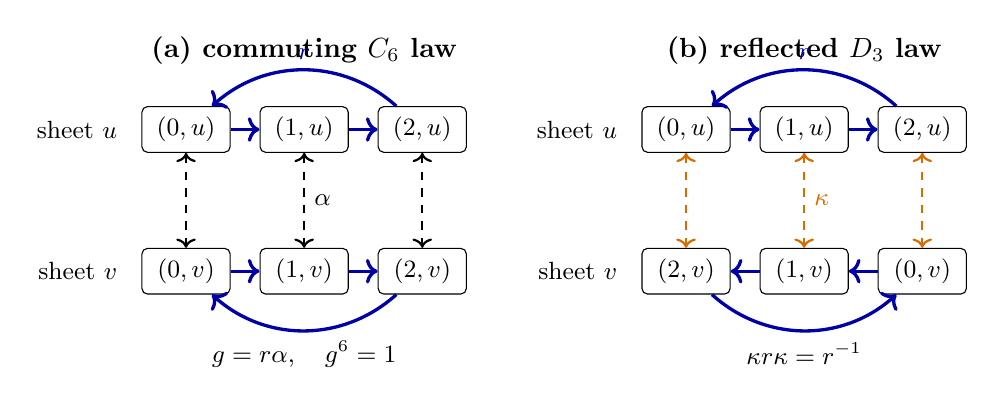
\begin{tikzpicture}[
  every node/.style={font=\small},
  cell/.style={
    draw,
    rounded corners=2pt,
    fill=white,
    minimum width=1.12cm,
    minimum height=0.58cm,
    inner sep=1.5pt
  },
  rot/.style={->,very thick,blue!65!black},
  sheet/.style={<->,thick,dashed,black},
  comp/.style={<->,thick,dashed,orange!85!black}
]
\begin{scope}
 \node[font=\bfseries] at (1.5,1.25) {(a) commuting \(C_6\) law};
 \node[anchor=east] at (-0.75,0.25) {sheet \(u\)};
 \node[anchor=east] at (-0.75,-1.55) {sheet \(v\)};
 \node[cell] (au0) at (0,0.25) {\((0,u)\)};
 \node[cell] (au1) at (1.5,0.25) {\((1,u)\)};
 \node[cell] (au2) at (3,0.25) {\((2,u)\)};
 \node[cell] (av0) at (0,-1.55) {\((0,v)\)};
 \node[cell] (av1) at (1.5,-1.55) {\((1,v)\)};
 \node[cell] (av2) at (3,-1.55) {\((2,v)\)};
 \draw[sheet] (au0) -- (av0);
 \draw[sheet] (au1) -- node[right] {\(\alpha\)} (av1);
 \draw[sheet] (au2) -- (av2);
 \draw[rot] (au0) -- (au1);
 \draw[rot] (au1) -- (au2);
 \draw[rot] (au2) to[bend right=42] node[above] {\(r\)} (au0);
 \draw[rot] (av0) -- (av1);
 \draw[rot] (av1) -- (av2);
 \draw[rot] (av2) to[bend left=42] (av0);
 \node at (1.5,-2.60) {\(g=r\alpha,\quad g^6=1\)};
\end{scope}
\begin{scope}[xshift=6.35cm]
 \node[font=\bfseries] at (1.5,1.25) {(b) reflected \(D_3\) law};
 \node[anchor=east] at (-0.75,0.25) {sheet \(u\)};
 \node[anchor=east] at (-0.75,-1.55) {sheet \(v\)};
 \node[cell] (bu0) at (0,0.25) {\((0,u)\)};
 \node[cell] (bu1) at (1.5,0.25) {\((1,u)\)};
 \node[cell] (bu2) at (3,0.25) {\((2,u)\)};
 \node[cell] (bv2) at (0,-1.55) {\((2,v)\)};
 \node[cell] (bv1) at (1.5,-1.55) {\((1,v)\)};
 \node[cell] (bv0) at (3,-1.55) {\((0,v)\)};
 \draw[comp] (bu0) -- (bv2);
 \draw[comp] (bu1) -- node[right] {\(\kappa\)} (bv1);
 \draw[comp] (bu2) -- (bv0);
 \draw[rot] (bu0) -- (bu1);
 \draw[rot] (bu1) -- (bu2);
 \draw[rot] (bu2) to[bend right=42] node[above] {\(r\)} (bu0);
 \draw[rot] (bv0) -- (bv1);
 \draw[rot] (bv1) -- (bv2);
 \draw[rot] (bv2) to[bend right=42] (bv0);
 \node at (1.5,-2.60) {\(\kappa r\kappa=r^{-1}\)};
\end{scope}
\end{tikzpicture}
\caption{The same six arithmetic cells support two different exact
couplings.  Blue arrows are the origin rotation \(r\).  In (a),
same-origin sheet exchange \(\alpha\) commutes with \(r\), and
\(r\alpha\) generates the regular \(C_6\)-action.  In (b), arithmetic
complement \(\kappa\) exchanges the sheets while reflecting the origin
coordinate, producing the regular \(D_3\)-action.}
\label{fig:coupled-packet-two-six-state-laws}
\end{figure}

\begin{corollary}[Arithmetic exhaustion and spectral splitting of the packet couplings]
\label{cor:coupled-packet-arithmetic-exhaustion-spectral-splitting}
Retain the conditions of
\cref{thm:coupled-packet-six-cell-laws}, choose one ordered sheet
\(\sigma\), and put
\[
 \mathcal C=C_3\times C_2.
\]
The map
\begin{equation}
 \Psi_\sigma:\mathcal C\longrightarrow\mathcal X(P),
 \qquad
 \Psi_\sigma(a,\epsilon)
 :=
 (a,u_{\iota^\epsilon\sigma})
 \label{eq:coupled-packet-carrier-bijection}
\end{equation}
is a bijection.  Let \(\circ\) and \(\star\) be the commuting and
reflected products from
\eqref{eq:C3-C2-commuting-product} and
\eqref{eq:C3-C2-reflected-product}.  If
\[
 x=(a,\epsilon),
 \qquad
 y=(b,\delta),
 \qquad
 \beta_P:=r_P\kappa_P,
\]
then
\begin{align}
 \Psi_\sigma(x\circ y)
 &=
 r_P^a\alpha_P^\epsilon\Psi_\sigma(y),
 \label{eq:coupled-packet-commuting-regular-identification}\\
 \Psi_\sigma(x\star y)
 &=
 r_P^a\beta_P^\epsilon\Psi_\sigma(y).
 \label{eq:coupled-packet-reflected-regular-identification}
\end{align}
Consequently these two arithmetic actions realize, and exhaust, the
two homomorphisms
\[
 C_2\longrightarrow\operatorname{Aut}(C_3).
\]

On \(\mathscr H_P\), put
\begin{equation}
 \mathbf P_{P,\pm}
 :=
 \frac12(I_{\mathscr H_P}\pm\mathbf A_P),
 \qquad
 \mathscr H_P^\pm:=\operatorname{im}\mathbf P_{P,\pm}.
 \label{eq:coupled-packet-sheet-parity-projections}
\end{equation}
These are orthogonal projections of rank three.  They commute with
\(\mathbf R_P\) and \(\mathbf K_P\).  For
\[
 \omega:=e^{2\pi i/3},
 \qquad
 \mathbf G_P:=\mathbf R_P\mathbf A_P,
\]
one has
\begin{equation}
 \operatorname{Spec}(\mathbf G_P)
 =
 \{1,-1,\omega,-\omega,\omega^2,-\omega^2\},
 \qquad
 \det(XI_6-\mathbf G_P)=X^6-1.
 \label{eq:coupled-packet-C6-simple-spectrum}
\end{equation}

Let \(V\) denote the two-dimensional irreducible complex
representation of \(D_3\).  Under the reflected packet action,
\begin{equation}
 \mathscr H_P^+\cong\mathbf 1\oplus V,
 \qquad
 \mathscr H_P^-\cong\operatorname{sgn}\oplus V,
 \qquad
 \mathscr H_P
 \cong
 \mathbf 1\oplus\operatorname{sgn}\oplus V^{\oplus2}.
 \label{eq:coupled-packet-D3-sheet-parity-decomposition}
\end{equation}
The trivial and sign lines are spanned respectively by
\begin{equation}
 c_P
 :=
 \sum_{j=0}^2
 (e_{j,\sigma}+e_{j,\iota\sigma}),
 \qquad
 s_P
 :=
 \sum_{j=0}^2
 (e_{j,\sigma}-e_{j,\iota\sigma}).
 \label{eq:coupled-packet-trivial-sign-vectors}
\end{equation}
\end{corollary}

\begin{proof}
The two sheet endpoints in
\eqref{eq:coupled-packet-complementary-endpoints} are distinct, and
each occurs once at every origin.  Hence
\eqref{eq:coupled-packet-carrier-bijection} is a bijection.  For the
commuting product,
\[
 r_P^a\alpha_P^\epsilon
 (b,u_{\iota^\delta\sigma})
 =
 (a+b,u_{\iota^{\epsilon+\delta}\sigma}),
\]
which is
\eqref{eq:coupled-packet-commuting-regular-identification}.  Since
\[
 \beta_P(j,u_\rho)
 =
 r_P(2-j,u_{\iota\rho})
 =
 (-j,u_{\iota\rho}),
\]
one likewise has
\[
 r_P^a\beta_P^\epsilon
 (b,u_{\iota^\delta\sigma})
 =
 (a+(-1)^\epsilon b,
   u_{\iota^{\epsilon+\delta}\sigma}),
\]
which proves
\eqref{eq:coupled-packet-reflected-regular-identification}.
\Cref{prop:C3-C2-two-couplings} proves exhaustion.

Equation
\eqref{eq:coupled-packet-positive-sheet-coupling} makes
\(\mathbf A_P\) a self-adjoint involution, so
\(\mathbf P_{P,\pm}\) are orthogonal projections.  The matrix
\(\mathbf A_P\) has zero diagonal and hence zero trace.  Therefore
\[
 \operatorname{tr}\mathbf P_{P,+}
 =
 \operatorname{tr}\mathbf P_{P,-}
 =
 3,
\]
which gives their ranks.  The first commutation follows from
\eqref{eq:coupled-packet-positive-sheet-coupling}; the second follows
from
\begin{equation}
 \mathbf A_P\mathbf K_P
 =
 \mathbf K_P\mathbf A_P
 =
 \begin{pmatrix}F_3&0\\0&F_3\end{pmatrix}.
 \label{eq:coupled-packet-sheet-complement-commutation}
\end{equation}

The eigenvalues of \(R_3\) are \(1,\omega,\omega^2\).  For each such
eigenvalue, the corresponding two-dimensional eigenspace of
\(\mathbf R_P\) contains one \(+1\) and one \(-1\) eigenline of
\(\mathbf A_P\), because \(\mathbf A_P\) exchanges the two sheets.
Thus \(\mathbf G_P=\mathbf R_P\mathbf A_P\) has the six eigenvalues in
\eqref{eq:coupled-packet-C6-simple-spectrum}, all with multiplicity
one.  Their product polynomial is \(X^6-1\).

The origin rotation fixes both vectors in
\eqref{eq:coupled-packet-trivial-sign-vectors}.  Arithmetic complement
fixes \(c_P\) and sends \(s_P\) to \(-s_P\).  Thus these vectors span
the trivial and sign representations.  The orthogonal complement of
\(\mathbb Cc_P\) in \(\mathscr H_P^+\) has dimension two, as does the
orthogonal complement of \(\mathbb Cs_P\) in \(\mathscr H_P^-\).
On each complement, \(\mathbf R_P\) has eigenvalues
\(\omega,\omega^2\).  Every one-dimensional representation of
\(D_3\) sends the order-three generator to \(1\), so neither complement
contains a one-dimensional subrepresentation.  Each is therefore
isomorphic to \(V\), proving
\eqref{eq:coupled-packet-D3-sheet-parity-decomposition}.
\end{proof}

\begin{theorem}[Packet parity is the tensor lift of the ordered blade supports]
\label{thm:packet-parity-tensor-lift-ordered-blade-supports}
Retain the conditions of
\cref{thm:coupled-packet-six-cell-laws} and choose one ordered sheet
\(\sigma\).  Let
\[
 \mathscr S_P
 :=
 \operatorname{span}_{\mathbb C}
 \{\eta_\sigma,\eta_{\iota\sigma}\},
 \qquad
 \mathscr O_3
 :=
 \operatorname{span}_{\mathbb C}\{f_0,f_1,f_2\},
\]
and define the unitary
\begin{equation}
 \Upsilon_\sigma:
 \mathscr S_P\otimes\mathscr O_3
 \longrightarrow\mathscr H_P,
 \qquad
 \Upsilon_\sigma(\eta_\rho\otimes f_j)
 :=
 e_{j,\rho}.
 \label{eq:packet-sheet-origin-tensor-identification}
\end{equation}
Then
\begin{equation}
 \begin{aligned}
  \Upsilon_\sigma^{-1}\mathbf A_P\Upsilon_\sigma
  &=S\otimes I_3,\\
  \Upsilon_\sigma^{-1}\mathbf R_P\Upsilon_\sigma
  &=I_2\otimes R_3,\\
  \Upsilon_\sigma^{-1}\mathbf K_P\Upsilon_\sigma
  &=S\otimes F_3.
 \end{aligned}
 \label{eq:packet-sheet-origin-tensor-factorization}
\end{equation}

Put
\[
 \eta_\pm
 :=
 \frac{\eta_\sigma\pm\eta_{\iota\sigma}}{\sqrt2},
\]
and define the lifted ordered blades
\begin{align}
 \mathbb B_{P,-+}
 &:=
 \Upsilon_\sigma
 \bigl((\eta_-\eta_+^\ast)\otimes I_3\bigr)
 \Upsilon_\sigma^{-1},
 \label{eq:packet-lifted-minus-plus-blade}\\
 \mathbb B_{P,+-}
 &:=
 \Upsilon_\sigma
 \bigl((\eta_+\eta_-^\ast)\otimes I_3\bigr)
 \Upsilon_\sigma^{-1}.
 \label{eq:packet-lifted-plus-minus-blade}
\end{align}
They are rank-three partial isometries with exact source and range
supports
\begin{align}
 \mathbb B_{P,-+}^\ast\mathbb B_{P,-+}
 &=\mathbf P_{P,+},
 &
 \mathbb B_{P,-+}\mathbb B_{P,-+}^\ast
 &=\mathbf P_{P,-},
 \label{eq:packet-minus-plus-source-range}\\
 \mathbb B_{P,+-}^\ast\mathbb B_{P,+-}
 &=\mathbf P_{P,-},
 &
 \mathbb B_{P,+-}\mathbb B_{P,+-}^\ast
 &=\mathbf P_{P,+}.
 \label{eq:packet-plus-minus-source-range}
\end{align}
Their ordered signs and origin covariance are
\begin{align}
 \mathbf A_P\mathbb B_{P,-+}
 &=-\mathbb B_{P,-+},
 &
 \mathbb B_{P,-+}\mathbf A_P
 &=\mathbb B_{P,-+},
 \label{eq:packet-minus-plus-ordered-signs}\\
 \mathbf A_P\mathbb B_{P,+-}
 &=\mathbb B_{P,+-},
 &
 \mathbb B_{P,+-}\mathbf A_P
 &=-\mathbb B_{P,+-},
 \label{eq:packet-plus-minus-ordered-signs}\\
 \mathbf R_P\mathbb B_{P,-+}
 &=
 \mathbb B_{P,-+}\mathbf R_P,
 &
 \mathbf R_P\mathbb B_{P,+-}
 &=
 \mathbb B_{P,+-}\mathbf R_P.
 \label{eq:packet-blade-origin-covariance}
\end{align}

Let \(U_\sigma:\mathbb C^2\to\mathscr S_P\) send the standard basis to
\((\eta_\sigma,\eta_{\iota\sigma})\), and let \(C_\sigma\) and
\(\Theta_\sigma\) be the exact flag maps in
\eqref{eq:coupled-packet-sheet-intertwiners}.  Define
\begin{equation}
 \mathfrak C_\sigma
 :=
 \Upsilon_\sigma
 \circ
 \bigl((U_\sigma C_\sigma)\otimes I_3\bigr).
 \label{eq:packet-flag-to-parity-intertwiner}
\end{equation}
Writing
\[
 \Pi_{\sigma,\pm}
 :=
 \Pi_{\pm,k_\sigma,q_\sigma},
\]
with the third parameter \(c=t\), one has
\begin{align}
 \mathfrak C_\sigma
 (\Theta_\sigma\otimes I_3)
 &=
 \mathbf A_P\mathfrak C_\sigma,
 \label{eq:packet-flag-involution-to-sheet-parity}\\
 \mathfrak C_\sigma
 (\Pi_{\sigma,\pm}\otimes I_3)
 &=
 \mathbf P_{P,\pm}\mathfrak C_\sigma,
 \label{eq:packet-flag-support-to-sheet-parity}\\
 \mathfrak C_\sigma
 (\mathscr D_\sigma\otimes I_3)
 \mathfrak C_\sigma^{-1}
 &=
 \frac{(p-1)t}{R}\,\mathbf A_P.
 \label{eq:packet-flag-defect-to-sheet-exchange}
\end{align}
For the complementary sheet \(\iota\sigma=(s,m,t)\), the corresponding
map obeys
\begin{equation}
 \mathfrak C_{\iota\sigma}
 (\mathscr D_{\iota\sigma}\otimes I_3)
 \mathfrak C_{\iota\sigma}^{-1}
 =
 \frac{(p-1)m}{R}\,\mathbf A_P.
 \label{eq:packet-complementary-flag-defect-to-sheet-exchange}
\end{equation}
Thus both flag defects determine the same packet involution, with their
positive arithmetic scales retained.

Finally, reversing the chosen sheet order fixes
\(\mathbf P_{P,+}\) and \(\mathbf P_{P,-}\), but sends
\begin{equation}
 \mathbb B_{P,-+}\longmapsto-\mathbb B_{P,-+},
 \qquad
 \mathbb B_{P,+-}\longmapsto-\mathbb B_{P,+-}.
 \label{eq:packet-blade-deck-orientation-sign}
\end{equation}
\end{theorem}

\begin{proof}
Equation
\eqref{eq:packet-sheet-origin-tensor-factorization} follows directly
from the three permutation matrices in
\eqref{eq:coupled-packet-six-cell-matrices}.  Under
\(\Upsilon_\sigma\), the packet parity projections are
\[
 \mathbf P_{P,\pm}
 =
 (\eta_\pm\eta_\pm^\ast)\otimes I_3.
\]
The source and range products in
\eqref{eq:packet-minus-plus-source-range} and
\eqref{eq:packet-plus-minus-source-range} are therefore the
rank-one identities from
\eqref{eq:mixer-minus-plus-supports} and
\eqref{eq:mixer-plus-minus-supports}, tensored with \(I_3\).
The bimodule signs follow in the same way from
\eqref{eq:mixer-minus-plus-bimodule-signs} and
\eqref{eq:mixer-plus-minus-bimodule-signs}.  Both lifted blades act as
the identity on \(\mathscr O_3\), which proves
\eqref{eq:packet-blade-origin-covariance}.

The sheet-basis map satisfies
\[
 U_\sigma S U_\sigma^{-1}
 =
 S_{\mathscr S_P},
\]
where \(S_{\mathscr S_P}\) exchanges
\(\eta_\sigma\) and \(\eta_{\iota\sigma}\).  Equation
\eqref{eq:coupled-packet-sheet-intertwining} consequently gives
\[
 (U_\sigma C_\sigma)\Theta_\sigma
 =
 S_{\mathscr S_P}(U_\sigma C_\sigma).
\]
Tensoring with \(I_3\) and applying \(\Upsilon_\sigma\) proves
\eqref{eq:packet-flag-involution-to-sheet-parity}.  Applying
\(\frac12(1\pm X)\) proves
\eqref{eq:packet-flag-support-to-sheet-parity}.  From
\eqref{eq:coupled-packet-sheet-defect} and
\eqref{eq:coupled-packet-sheet-intertwiners},
\[
 \mathscr D_\sigma
 =
 \frac{(p-1)t}{R}\,\Theta_\sigma.
\]
This proves
\eqref{eq:packet-flag-defect-to-sheet-exchange}; exchanging \(t\) and
\(m\) proves
\eqref{eq:packet-complementary-flag-defect-to-sheet-exchange}.

Under \(\sigma\leftrightarrow\iota\sigma\), the vector \(\eta_+\) is
fixed and \(\eta_-\) changes sign.  The two parity projectors are
therefore fixed, while each rank-one ordered blade changes sign.  This
proves
\eqref{eq:packet-blade-deck-orientation-sign}.
\end{proof}

\begin{theorem}[Exact transition between the complementary packet flags]
\label{thm:complementary-packet-exact-flag-transition}
Retain the conditions of
\cref{thm:packet-parity-tensor-lift-ordered-blade-supports}.  Write
\[
 h_\sigma:=k_\sigma+q_\sigma,
 \qquad
 h_{\iota\sigma}:=k_{\iota\sigma}+q_{\iota\sigma},
 \qquad
 h_P:=h_\sigma+h_{\iota\sigma},
\]
where \(\sigma=(s,t,m)\) and \(\iota\sigma=(s,m,t)\).  The transition
from the \(\sigma\)-flag coordinates to the
\(\iota\sigma\)-flag coordinates is
\begin{equation}
 \begin{split}
 \mathcal T_{\sigma\to\iota\sigma}
 &:=
 \mathfrak C_{\iota\sigma}^{-1}\mathfrak C_\sigma
 =
 T_{\sigma\to\iota\sigma}\otimes I_3,\\
 T_{\sigma\to\iota\sigma}
 &:=
 C_{\iota\sigma}^{-1}SC_\sigma
 =
 \begin{pmatrix}
  -1&\dfrac{h_P}{2t}\\[2mm]
  0&\dfrac mt
 \end{pmatrix}.
 \end{split}
 \label{eq:complementary-packet-flag-transition}
\end{equation}
The reverse transition is
\begin{equation}
 T_{\iota\sigma\to\sigma}
 =
 \begin{pmatrix}
  -1&\dfrac{h_P}{2m}\\[2mm]
  0&\dfrac tm
 \end{pmatrix}
 =
 T_{\sigma\to\iota\sigma}^{-1}.
 \label{eq:complementary-packet-reverse-flag-transition}
\end{equation}
In particular,
\begin{equation}
 \det T_{\sigma\to\iota\sigma}=-\frac mt,
 \qquad
 \operatorname{Spec}(T_{\sigma\to\iota\sigma})
 =
 \left\{-1,\frac mt\right\}.
 \label{eq:complementary-packet-flag-transition-spectrum}
\end{equation}
The two eigenlines are generated by
\begin{equation}
 \begin{pmatrix}1\\0\end{pmatrix},
 \qquad
 \begin{pmatrix}\dfrac{h_P}{2(t+m)}\\[1mm]1\end{pmatrix},
 \label{eq:complementary-packet-flag-transition-eigenlines}
\end{equation}
with eigenvalues \(-1\) and \(m/t\), respectively.  Since the deck
action is free, \(t\ne m\).  On the six-dimensional flag carrier,
\(-1\) and \(m/t\) each have multiplicity three and
\[
 \det\mathcal T_{\sigma\to\iota\sigma}
 =
 -\left(\frac mt\right)^3.
\]

Put
\[
 \Pi_{\rho,\pm}:=\Pi_{\pm,k_\rho,q_\rho}
 \qquad
 (\rho\in\{\sigma,\iota\sigma\}).
\]
The transition preserves the ordered support labels:
\begin{align}
 \mathcal T_{\sigma\to\iota\sigma}
 (\Theta_\sigma\otimes I_3)
 &=
 (\Theta_{\iota\sigma}\otimes I_3)
 \mathcal T_{\sigma\to\iota\sigma},
 \label{eq:complementary-packet-transition-involution}\\
 \mathcal T_{\sigma\to\iota\sigma}
 (\Pi_{\sigma,\pm}\otimes I_3)
 &=
 (\Pi_{\iota\sigma,\pm}\otimes I_3)
 \mathcal T_{\sigma\to\iota\sigma}.
 \label{eq:complementary-packet-transition-supports}
\end{align}
The reverse-channel defects retain their unequal arithmetic scales:
\begin{equation}
 \mathcal T_{\sigma\to\iota\sigma}
 (\mathscr D_\sigma\otimes I_3)
 =
 \frac tm
 (\mathscr D_{\iota\sigma}\otimes I_3)
 \mathcal T_{\sigma\to\iota\sigma}.
 \label{eq:complementary-packet-transition-defects}
\end{equation}

The corresponding transport on packet space is
\[
 \mathcal P_{\sigma\to\iota\sigma}
 :=
 \mathfrak C_{\iota\sigma}\mathfrak C_\sigma^{-1}.
\]
Put
\[
 \widehat\Upsilon_\sigma
 :=
 \Upsilon_\sigma\circ(U_\sigma\otimes I_3).
\]
In the ordered sheet basis
\((\eta_\sigma,\eta_{\iota\sigma})\), put
\[
 r:=\frac tm,
 \qquad
 d:=h_\sigma-rh_{\iota\sigma}.
\]
Then
\begin{equation}
 \widehat\Upsilon_\sigma^{-1}
 \mathcal P_{\sigma\to\iota\sigma}
 \widehat\Upsilon_\sigma
 =
 L_{\sigma\to\iota\sigma}\otimes I_3,
 \qquad
 L_{\sigma\to\iota\sigma}
 =
 \frac12
 \begin{pmatrix}
  r-d-1&r-d+1\\
  r+d+1&r+d-1
 \end{pmatrix}.
 \label{eq:complementary-packet-packet-space-transport}
\end{equation}
Consequently,
\begin{equation}
 \det L_{\sigma\to\iota\sigma}=-\frac tm,
 \qquad
 \operatorname{Spec}(L_{\sigma\to\iota\sigma})
 =
 \left\{-1,\frac tm\right\}.
 \label{eq:complementary-packet-packet-space-spectrum}
\end{equation}
Thus both the flag-coordinate transition and the packet-space
transport have one negative direction and one positive scale direction;
the scale is reciprocal between the two realizations.
\end{theorem}

\begin{proof}
For \(h=x+y\), the matrices in
\eqref{eq:carrier-half-period-intertwiner-matrix} obey
\[
 F_{x,y,c}
 =
 \begin{pmatrix}
  0&\dfrac1{2c}\\[1mm]
  1&-\dfrac h{2c}
 \end{pmatrix},
 \qquad
 F_{x,y,c}^{-1}
 =
 \begin{pmatrix}h&1\\2c&0\end{pmatrix}.
\]
The unitary in
\eqref{eq:packet-sheet-origin-tensor-identification} is unchanged as
an actual map when the two sheet labels are reversed, while
\(U_{\iota\sigma}=U_\sigma S\).  Hence
\[
 \mathfrak C_{\iota\sigma}^{-1}\mathfrak C_\sigma
 =
 \bigl(C_{\iota\sigma}^{-1}SC_\sigma\bigr)\otimes I_3.
\]
Using \(C_\rho=HF_\rho\) and \(HSH=J\) gives
\[
 C_{\iota\sigma}^{-1}SC_\sigma
 =
 F_{\iota\sigma}^{-1}JF_\sigma.
\]
Substitution of the two displayed inverse matrices gives
\eqref{eq:complementary-packet-flag-transition}.  Exchanging \(t\) and
\(m\) gives
\eqref{eq:complementary-packet-reverse-flag-transition}; direct
multiplication gives both inverse identities.  The matrix is upper
triangular, which proves
\eqref{eq:complementary-packet-flag-transition-spectrum}.  Applying it
to the two vectors in
\eqref{eq:complementary-packet-flag-transition-eigenlines} proves the
eigenline statement.  Tensoring with \(I_3\) gives the multiplicities
and determinant on the full flag carrier.

From
\eqref{eq:coupled-packet-sheet-intertwining},
\[
 T_{\sigma\to\iota\sigma}\Theta_\sigma
 =
 C_{\iota\sigma}^{-1}SC_\sigma\Theta_\sigma
 =
 C_{\iota\sigma}^{-1}C_\sigma
 =
 \Theta_{\iota\sigma}
 T_{\sigma\to\iota\sigma}.
\]
This proves
\eqref{eq:complementary-packet-transition-involution}.  Applying
\(\frac12(1\pm X)\) proves
\eqref{eq:complementary-packet-transition-supports}.  Finally,
\[
 \mathscr D_\sigma
 =
 \frac{(p-1)t}{R}\Theta_\sigma,
 \qquad
 \mathscr D_{\iota\sigma}
 =
 \frac{(p-1)m}{R}\Theta_{\iota\sigma},
\]
so the involution intertwining gives
\eqref{eq:complementary-packet-transition-defects}.

For the packet-space transport,
\[
 \widehat\Upsilon_\sigma^{-1}
 \mathcal P_{\sigma\to\iota\sigma}
 \widehat\Upsilon_\sigma
 =
 \bigl(SC_{\iota\sigma}C_\sigma^{-1}\bigr)\otimes I_3.
\]
The intermediate flag product is
\[
 F_{\iota\sigma}F_\sigma^{-1}
 =
 \begin{pmatrix}r&0\\d&1\end{pmatrix}.
\]
Since \(SH=HJ\),
\[
 SC_{\iota\sigma}C_\sigma^{-1}
 =
 HJ
 \begin{pmatrix}r&0\\d&1\end{pmatrix}
 H,
\]
and multiplication gives the matrix in
\eqref{eq:complementary-packet-packet-space-transport}.  Its trace is
\(r-1\) and its determinant is \(-r\), proving
\eqref{eq:complementary-packet-packet-space-spectrum}.
\end{proof}

\begin{theorem}[Canonical fixed line of an unordered arithmetic packet]
\label{thm:unordered-packet-canonical-fixed-line}
Retain the conditions of
\cref{thm:complementary-packet-exact-flag-transition}.  Put
\begin{equation}
 \delta_P:=\frac{p-1}{R},
 \qquad
 \ell_P:=\frac{t+m}{R}.
 \label{eq:unordered-packet-delta-ell}
\end{equation}
These are positive integers.  The positive transition eigenline has the
order-independent coordinate
\begin{equation}
 \gamma_P
 :=
 \frac{h_P}{2(t+m)}
 =
 4s\ell_P
 -
 \frac{\delta_P+2}{\ell_PR},
 \qquad
 w_P:=
 \begin{pmatrix}\gamma_P\\1\end{pmatrix}.
 \label{eq:unordered-packet-gamma}
\end{equation}
In particular,
\[
 0<\gamma_P<4s\ell_P,
\]
and
\begin{equation}
 T_{\sigma\to\iota\sigma}w_P=\frac mtw_P,
 \qquad
 T_{\iota\sigma\to\sigma}w_P=\frac tmw_P.
 \label{eq:unordered-packet-fixed-projective-line}
\end{equation}

Define the oriented coordinate
\begin{equation}
 \mu_\sigma
 :=
 \frac{(m-t)(\delta_P+2)}{t+m}.
 \label{eq:unordered-packet-oriented-coordinate}
\end{equation}
Then \(\mu_{\iota\sigma}=-\mu_\sigma\), and the vector
\begin{equation}
 v_P
 :=
 (1+\mu_\sigma)\eta_\sigma
 +
 (1-\mu_\sigma)\eta_{\iota\sigma}
 \in\mathscr S_P
 \label{eq:unordered-packet-fixed-vector}
\end{equation}
is unchanged when the ordered sheet \(\sigma\) is replaced by
\(\iota\sigma\).  The two flag charts map \(w_P\) to the same line in
\(\mathscr S_P\), with exact scale factors
\begin{equation}
 U_\sigma C_\sigma w_P
 =
 \frac{1}{2\sqrt2\,t}v_P,
 \qquad
 U_{\iota\sigma}C_{\iota\sigma}w_P
 =
 \frac{1}{2\sqrt2\,m}v_P.
 \label{eq:unordered-packet-fixed-vector-chart-images}
\end{equation}

Let \(Q_P^{\mathrm{fix}}\) be the rank-one orthogonal projection onto
\(\mathbb Cv_P\), and lift it to the six-dimensional packet carrier by
\[
 \mathbb Q_P^{\mathrm{fix}}
 :=
 \Upsilon_\sigma
 \bigl(Q_P^{\mathrm{fix}}\otimes I_3\bigr)
 \Upsilon_\sigma^{-1}.
\]
This rank-three orthogonal projection is independent of the chosen
ordered sheet and has the exact ordered-blade expansion
\begin{equation}
 \mathbb Q_P^{\mathrm{fix}}
 =
 \frac{1}{1+\mu_\sigma^2}
 \left(
  \mathbf P_{P,+}
  +
  \mu_\sigma
  \bigl(\mathbb B_{P,-+}+\mathbb B_{P,+-}\bigr)
  +
  \mu_\sigma^2\mathbf P_{P,-}
 \right).
 \label{eq:unordered-packet-fixed-projection-blade-expansion}
\end{equation}
It commutes with the arithmetic-origin rotation.  Its commutator with
sheet exchange is
\begin{equation}
 [\mathbf A_P,\mathbb Q_P^{\mathrm{fix}}]
 =
 \frac{2\mu_\sigma}{1+\mu_\sigma^2}
 \bigl(\mathbb B_{P,+-}-\mathbb B_{P,-+}\bigr)
 \ne0.
 \label{eq:unordered-packet-fixed-projection-commutator}
\end{equation}
Thus the order-independent packet line is neither pure positive parity
nor pure negative parity: its exact off-diagonal part is carried by the
two ordered blade channels.
\end{theorem}

\begin{proof}
The coupled-shell conditions give
\[
 R\mid p-1,
 \qquad
 R\mid t+m,
\]
which proves the integrality in
\eqref{eq:unordered-packet-delta-ell}.  Since
\[
 p=4stm-R,
 \qquad
 t+m=\ell_PR,
\]
the sheet data in \eqref{eq:coupled-packet-sheet-data} satisfy
\begin{align*}
 q_\sigma
 &=
 \frac{p+4st^2}{R}
 =
 4s\ell_Pt-1,\\
 q_{\iota\sigma}
 &=
 \frac{p+4sm^2}{R}
 =
 4s\ell_Pm-1,
\end{align*}
and
\[
 q_\rho-k_\rho
 =
 \frac{p-1}{R}
 =
 \delta_P
 \qquad
 (\rho\in\{\sigma,\iota\sigma\}).
\]
Therefore
\[
 h_\rho=2q_\rho-\delta_P
\]
and
\begin{equation}
 h_P
 =
 2\bigl(4s\ell_P^2R-\delta_P-2\bigr).
 \label{eq:unordered-packet-total-height}
\end{equation}
Division by \(2(t+m)=2\ell_PR\) proves
\eqref{eq:unordered-packet-gamma}.  Its positivity follows from
\(h_P>0\); the displayed correction to \(4s\ell_P\) is positive, which
proves the strict upper bound.  Equation
\eqref{eq:unordered-packet-fixed-projective-line} follows from
\eqref{eq:complementary-packet-flag-transition} and
\eqref{eq:complementary-packet-reverse-flag-transition}.

Apply the two matrices
\(F_\sigma=F_{k_\sigma,q_\sigma,t}\) and
\(F_{\iota\sigma}=F_{k_{\iota\sigma},q_{\iota\sigma},m}\) to \(w_P\).
Using \(h_P=h_\sigma+h_{\iota\sigma}\) gives
\begin{align*}
 F_\sigma w_P
 &=
 \frac1{2t}
 \begin{pmatrix}
  1\\[1mm]
  \dfrac{th_{\iota\sigma}-mh_\sigma}{t+m}
 \end{pmatrix},\\
 F_{\iota\sigma}w_P
 &=
 \frac1{2m}
 \begin{pmatrix}
  1\\[1mm]
  \dfrac{mh_\sigma-th_{\iota\sigma}}{t+m}
 \end{pmatrix}.
\end{align*}
The formulas just proved for the two heights give
\[
 th_{\iota\sigma}-mh_\sigma
 =
 (m-t)(\delta_P+2).
\]
Hence
\begin{equation}
 F_\sigma w_P
 =
 \frac1{2t}
 \begin{pmatrix}1\\\mu_\sigma\end{pmatrix},
 \qquad
 F_{\iota\sigma}w_P
 =
 \frac1{2m}
 \begin{pmatrix}1\\-\mu_\sigma\end{pmatrix}.
 \label{eq:unordered-packet-half-period-images}
\end{equation}
Applying the Hadamard matrix \(H\), followed by the two ordered sheet
maps, proves
\eqref{eq:unordered-packet-fixed-vector-chart-images}.  Exchanging
\(t\) and \(m\) changes the sign of \(\mu_\sigma\) and exchanges
\(\eta_\sigma,\eta_{\iota\sigma}\), so
\eqref{eq:unordered-packet-fixed-vector} is unchanged.

In the parity basis,
\[
 v_P
 =
 \sqrt2\bigl(\eta_++\mu_\sigma\eta_-\bigr),
 \qquad
 \langle v_P,v_P\rangle
 =
 2(1+\mu_\sigma^2).
\]
The rank-one projection onto this line is therefore
\[
 Q_P^{\mathrm{fix}}
 =
 \frac{1}{1+\mu_\sigma^2}
 \left(
  \eta_+\eta_+^\ast
  +
  \mu_\sigma
  \bigl(\eta_-\eta_+^\ast+\eta_+\eta_-^\ast\bigr)
  +
  \mu_\sigma^2\eta_-\eta_-^\ast
 \right).
\]
Tensoring with \(I_3\) and applying \(\Upsilon_\sigma\) proves
\eqref{eq:unordered-packet-fixed-projection-blade-expansion}.  Each
term commutes with \(\mathbf R_P\).  Reversing the sheet order changes
the signs of both \(\mu_\sigma\) and the two directed blades, and hence
fixes the displayed projection.

In the parity basis, sheet exchange is
\(\operatorname{diag}(1,-1)\).  Direct multiplication gives
\[
 [\mathbf A_P,\mathbb Q_P^{\mathrm{fix}}]
 =
 \frac{2\mu_\sigma}{1+\mu_\sigma^2}
 \bigl(\mathbb B_{P,+-}-\mathbb B_{P,-+}\bigr).
\]
The packet action is free, so \(t\ne m\), and therefore
\(\mu_\sigma\ne0\).  This proves
\eqref{eq:unordered-packet-fixed-projection-commutator}.
\end{proof}

\begin{theorem}[Square-discriminant reconstruction and the packet quarter]
\label{thm:unordered-packet-square-discriminant-quarter}
Retain the conditions of
\cref{cor:coupled-packet-two-sheet-flag-family}.  Define
\begin{equation}
 \mathscr D_{R,a}
 :=
 \left\{
  (s,\ell):
  \begin{array}{c}
   s\mid a,\quad s\ \text{squarefree},\quad
   \ell\in\mathbb Z_{>0},\\[1mm]
   D_{s,\ell}:=\ell^2R^2-\dfrac{4a}{s}
   \ \text{is a positive square}
  \end{array}
 \right\}.
 \label{eq:packet-square-discriminant-set}
\end{equation}
The map
\begin{equation}
 \begin{split}
 \Phi_{R,a}\colon\mathcal T_{R,a}
 &\longrightarrow\mathscr D_{R,a},\\
 (s,\{t,m\})
 &\longmapsto
 \left(s,\frac{t+m}{R}\right)
 \end{split}
 \label{eq:packet-square-discriminant-map}
\end{equation}
is a bijection.  If \(d_{s,\ell}:=\sqrt{D_{s,\ell}}>0\), its inverse is
\begin{equation}
 (s,\ell)
 \longmapsto
 \left(
  s,
  \left\{
   \frac{\ell R-d_{s,\ell}}2,
   \frac{\ell R+d_{s,\ell}}2
  \right\}
 \right).
 \label{eq:packet-square-discriminant-inverse}
\end{equation}
Every pair in \(\mathscr D_{R,a}\) satisfies
\begin{equation}
 \ell R\le\frac as+1.
 \label{eq:packet-square-discriminant-bound}
\end{equation}
Consequently,
\begin{equation}
 |\mathcal T_{R,a}|
 =
 \sum_{\substack{s\mid a\\s\ {\rm squarefree}}}
 \#\left\{
  \ell\in\mathbb Z_{>0}:
  \begin{array}{c}
   \ell R\le a/s+1,\\
   \ell^2R^2-4a/s\ \text{is a positive square}
  \end{array}
 \right\}.
 \label{eq:packet-square-discriminant-count}
\end{equation}

For an ordered sheet \(\sigma=(s,t,m)\) over
\(P=(s,\{t,m\})\), put
\begin{equation}
 \vartheta_\sigma:=\frac{t}{t+m},
 \qquad
 r_\sigma:=\frac{t-m}{t+m},
 \qquad
 \zeta_P:=-\frac{tm}{(t+m)^2}.
 \label{eq:packet-quarter-coordinates}
\end{equation}
Then
\begin{align}
 D_{s,\ell_P}
 &=(t-m)^2,
 &
 r_\sigma^2
 &=\frac{D_{s,\ell_P}}{\ell_P^2R^2},
 \label{eq:packet-discriminant-centered-coordinate}\\
 \mu_\sigma
 &=-(\delta_P+2)r_\sigma,
 &
 \zeta_P
 &=
 -\frac14+\frac{r_\sigma^2}{4}.
 \label{eq:packet-oriented-quarter-coordinate}
\end{align}
In particular, the fixed-line coordinate of
\cref{thm:unordered-packet-canonical-fixed-line} determines the exact
distance from the branch value in \cref{thm:ES-quarter-branch}:
\begin{equation}
 \boxed{
  \zeta_P+\frac14
  =
  \frac{D_{s,\ell_P}}{4\ell_P^2R^2}
  =
  \frac{\mu_\sigma^2}{4(\delta_P+2)^2}
 }.
 \label{eq:packet-fixed-line-quarter-identity}
\end{equation}
Moreover,
\begin{equation}
 -\frac14<\zeta_P<0.
 \label{eq:packet-quarter-open-interval}
\end{equation}
\end{theorem}

\begin{proof}
Let \(P=(s,\{t,m\})\in\mathcal T_{R,a}\).  By
\cref{eq:coupled-channel-equivalence},
\[
 t+m=\ell_PR,
 \qquad
 tm=\frac as.
\]
Thus \(t\) and \(m\) are the roots of
\[
 X^2-\ell_PRX+\frac as,
\]
whose discriminant is
\[
 \ell_P^2R^2-\frac{4a}{s}=(t-m)^2>0.
\]
This proves that \(\Phi_{R,a}\) maps into
\(\mathscr D_{R,a}\).

Conversely, let \((s,\ell)\in\mathscr D_{R,a}\), and write
\(d=\sqrt{D_{s,\ell}}\).  Since
\[
 d^2\equiv\ell^2R^2\pmod4,
\]
the integers \(d\) and \(\ell R\) have the same parity.  Also
\[
 0<d^2=\ell^2R^2-\frac{4a}{s}<\ell^2R^2,
\]
so the two numbers in
\eqref{eq:packet-square-discriminant-inverse} are distinct positive
integers.  Their sum is \(\ell R\), and their product is
\[
 \frac{(\ell R-d)(\ell R+d)}4
 =
 \frac{\ell^2R^2-d^2}{4}
 =
 \frac as.
\]
Hence they produce a squarefree coordinate \(a=stm\) with
\(R\mid t+m\).  The equivalence
\eqref{eq:coupled-channel-equivalence} places the resulting unordered
triple in \(\mathcal T_{R,a}\).  The sum and product recover the same
quadratic polynomial, so the two constructions are inverse.

For positive integers \(t,m\),
\[
 t+m\le tm+1,
\]
because \((t-1)(m-1)\ge0\).  This proves
\eqref{eq:packet-square-discriminant-bound}, and the bijection gives
\eqref{eq:packet-square-discriminant-count}.

Apply \cref{thm:ES-quarter-branch} with \(b=t\) and \(c=m\).  Its
centered branch coordinate is \(r_\sigma\), and direct expansion gives
\[
 -\vartheta_\sigma(1-\vartheta_\sigma)
 =
 -\frac{tm}{(t+m)^2}
 =
 -\frac14+\frac{(t-m)^2}{4(t+m)^2}.
\]
The discriminant identity and \(t+m=\ell_PR\) prove
\eqref{eq:packet-discriminant-centered-coordinate}.  The definition
\eqref{eq:unordered-packet-oriented-coordinate} gives
\[
 \mu_\sigma
 =
 \frac{(m-t)(\delta_P+2)}{t+m}
 =
 -(\delta_P+2)r_\sigma.
\]
Substitution proves
\eqref{eq:packet-oriented-quarter-coordinate} and
\eqref{eq:packet-fixed-line-quarter-identity}.  Finally \(tm>0\)
gives \(\zeta_P<0\), while \(t\ne m\) makes the final two terms in
\eqref{eq:packet-fixed-line-quarter-identity} positive.  This proves
\eqref{eq:packet-quarter-open-interval}.
\end{proof}

\begin{theorem}[Cartesian packet cover and the Fable quarter endpoints]
\label{thm:packet-cartesian-cover-fable-endpoints}
Retain the conditions of
\cref{thm:unordered-packet-square-discriminant-quarter}.  Regard the two
finite sets as finite reduced \(\Q\)-schemes
\[
 \mathbf S_{R,a}
 :=
 \coprod_{\sigma\in\mathcal S^{\mathrm{ext}}_{R,a}}
 \operatorname{Spec}\Q,
 \qquad
 \mathbf T_{R,a}
 :=
 \coprod_{P\in\mathcal T_{R,a}}
 \operatorname{Spec}\Q.
\]
Let
\begin{equation}
 q\colon\mathbb A^1_y\longrightarrow\mathbb A^1_\zeta,
 \qquad
 q(y):=-\frac14+\frac{y^2}{4},
 \label{eq:universal-quarter-cover}
\end{equation}
and define
\begin{equation}
 y_{R,a}(\sigma)
 :=
 \frac{\mu_\sigma}{\delta_{\pi_{R,a}(\sigma)}+2}
 =
 \frac{m-t}{m+t},
 \qquad
 \zeta_{R,a}(P):=\zeta_P.
 \label{eq:packet-cover-coordinate-map}
\end{equation}
Then the square
\begin{equation}
 \begin{array}{ccc}
  \mathbf S_{R,a}
  &\xrightarrow{\ y_{R,a}\ }&
  \mathbb A^1_y\\[1mm]
  {\scriptstyle\pi_{R,a}}\downarrow
  &&
  \downarrow{\scriptstyle q}\\[1mm]
  \mathbf T_{R,a}
  &\xrightarrow{\ \zeta_{R,a}\ }&
  \mathbb A^1_\zeta
 \end{array}
 \label{eq:packet-quarter-cartesian-square}
\end{equation}
is cartesian.  Equivalently,
\begin{equation}
 \mathbf S_{R,a}
 \cong
 \mathbf T_{R,a}
 \mathbin{\times}_{\mathbb A^1_\zeta}
 \mathbb A^1_y.
 \label{eq:packet-quarter-fibre-product}
\end{equation}
Under this isomorphism, the deck involution \(\iota\) is \(y\mapsto-y\).
The pullback is finite \'etale: its two points over \(P\) have coordinates
\begin{equation}
 y=\pm\frac{d_{s,\ell_P}}{\ell_PR},
 \label{eq:packet-cover-two-roots}
\end{equation}
and neither coordinate is zero.

Put
\begin{equation}
 h(y):=\frac{y^2}{4}.
 \label{eq:universal-quarter-height}
\end{equation}
Every ordered arithmetic sheet satisfies
\begin{equation}
 0<h\bigl(y_{R,a}(\sigma)\bigr)<\frac14,
 \qquad
 \zeta_{\pi_{R,a}(\sigma)}
 =
 -\frac14+h\bigl(y_{R,a}(\sigma)\bigr).
 \label{eq:packet-cover-open-height}
\end{equation}

On the complete Fable fibre of \cref{thm:Fable-fibre}, let
\(x\) denote the first source coordinate.  Its exact values under the
same two morphisms are
\begin{equation}
 \begin{array}{c|ccc}
  p&p_0&p_+&p_-\\ \hline
  x(p)&0&1&-1\\
  h(x(p))&0&\frac14&\frac14\\
  q(x(p))&-\frac14&0&0\\
  F_1(p)&-\frac14&-\frac14&-\frac14
 \end{array}.
 \label{eq:fable-quarter-endpoint-table}
\end{equation}
In particular,
\begin{equation}
 q(x(p))-F_1(p)=h(x(p))
 \qquad
 (p\in\{p_0,p_+,p_-\}).
 \label{eq:fable-quarter-height-defect}
\end{equation}
Thus the fixed Fable point realizes height \(0\), its transposed pair
realizes height \(1/4\), and every primitive coupled arithmetic packet
lies strictly between these two endpoint heights.
\end{theorem}

\begin{proof}
The relation between \(\mu_\sigma\) and the centered packet coordinate
in \eqref{eq:packet-oriented-quarter-coordinate} gives
\[
 y_{R,a}(\sigma)
 =
 -r_\sigma
 =
 \frac{m-t}{m+t}.
\]
Consequently,
\[
 q\bigl(y_{R,a}(\sigma)\bigr)
 =
 -\frac14+\frac{(m-t)^2}{4(m+t)^2}
 =
 -\frac{tm}{(t+m)^2}
 =
 \zeta_{\pi_{R,a}(\sigma)}.
\]
This proves commutativity of
\eqref{eq:packet-quarter-cartesian-square}, and exchanging \(t\) with
\(m\) sends \(y\) to \(-y\).

Fix \(P=(s,\{t,m\})\).  The coordinate algebra of the fibre product
over this component is
\begin{align*}
 \Q[Y]\big/\bigl(Y^2-(1+4\zeta_P)\bigr)
 &=
 \Q[Y]\big/\bigl(Y^2-y_{R,a}(\sigma)^2\bigr)\\
 &=
 \Q[Y]\big/
 \bigl((Y-y_{R,a}(\sigma))(Y+y_{R,a}(\sigma))\bigr).
\end{align*}
The coordinate \(y_{R,a}(\sigma)\) is nonzero because \(t\ne m\).
The two linear factors are therefore coprime, so the Chinese remainder
theorem identifies this algebra with \(\Q\oplus\Q\).  Its two rational
points are exactly \(\sigma\) and \(\iota\sigma\).  Applying this on
every component proves \eqref{eq:packet-quarter-fibre-product}.
Moreover,
\[
 y_{R,a}(\sigma)^2
 =
 \frac{D_{s,\ell_P}}{\ell_P^2R^2},
\]
which proves \eqref{eq:packet-cover-two-roots}.  Since
\(q'(y)=y/2\), the cover is ramified only at \(y=0\); the arithmetic
pullback avoids that point and is finite \'etale.

Positivity of \(t\) and \(m\), together with \(t\ne m\), gives
\[
 0<|m-t|<m+t.
\]
This proves \eqref{eq:packet-cover-open-height}.  Finally, the source
coordinates in \eqref{eq:F-preimages} give
\(x(p_0)=0\), \(x(p_+)=1\), and \(x(p_-)=-1\), while
\eqref{eq:F-common-image} gives \(F_1(p)=-1/4\) at all three points.
Substitution into \eqref{eq:universal-quarter-cover} and
\eqref{eq:universal-quarter-height} proves
\eqref{eq:fable-quarter-endpoint-table} and
\eqref{eq:fable-quarter-height-defect}.
\end{proof}

\begin{figure}[ht]
\centering
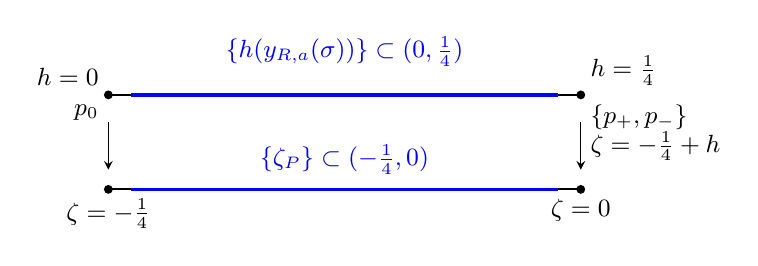
\begin{tikzpicture}[x=24cm,y=1cm,>=stealth,font=\small]
 \draw[thick] (0,1.2)--(0.25,1.2);
 \fill (0,1.2) circle (1.6pt);
 \fill (0.25,1.2) circle (1.6pt);
 \draw[very thick,blue] (0.012,1.2)--(0.238,1.2);
 \node[above left] at (0,1.2) {\(h=0\)};
 \node[above right] at (0.25,1.2) {\(h=\frac14\)};
 \node[below left] at (0,1.2) {\(p_0\)};
 \node[below right] at (0.25,1.2) {\(\{p_+,p_-\}\)};
 \node[blue] at (0.125,1.75)
 {\(\{h(y_{R,a}(\sigma))\}\subset(0,\frac14)\)};

 \draw[->] (0,0.85)--(0,0.25);
 \draw[->] (0.25,0.85)--(0.25,0.25);
 \node[right] at (0.25,0.55) {\(\zeta=-\frac14+h\)};

 \draw[thick] (0,0)--(0.25,0);
 \fill (0,0) circle (1.6pt);
 \fill (0.25,0) circle (1.6pt);
 \draw[very thick,blue] (0.012,0)--(0.238,0);
 \node[below] at (0,0) {\(\zeta=-\frac14\)};
 \node[below] at (0.25,0) {\(\zeta=0\)};
 \node[blue] at (0.125,0.38)
 {\(\{\zeta_P\}\subset(-\frac14,0)\)};
\end{tikzpicture}
\caption{The universal quarter height.  The Fable fibre supplies the two
endpoint heights; primitive coupled arithmetic packets occupy the open
height interval and map to the open \(\zeta\)-interval.}
\label{fig:packet-fable-quarter-height}
\end{figure}

\begin{theorem}[Blade-coupling formula for the packet quarter height]
\label{thm:packet-blade-coupling-quarter-height}
Retain the conditions of
\cref{thm:unordered-packet-canonical-fixed-line} and
\cref{thm:unordered-packet-square-discriminant-quarter}.  On the
two-dimensional parity space \(\mathscr S_P\), put
\[
 E_+:=\eta_+\eta_+^\ast,
 \qquad
 E_-:=\eta_-\eta_-^\ast,
 \qquad
 Q:=Q_P^{\mathrm{fix}},
 \qquad
 S:=E_+-E_-,
\]
and define
\begin{equation}
 a_\pm(P):=\operatorname{tr}(E_\pm Q).
 \label{eq:packet-parity-fixed-line-weights}
\end{equation}
Then
\begin{equation}
 a_+(P)=\frac{1}{1+\mu_\sigma^2},
 \qquad
 a_-(P)=\frac{\mu_\sigma^2}{1+\mu_\sigma^2},
 \qquad
 a_+(P)+a_-(P)=1,
 \label{eq:packet-parity-weight-formulas}
\end{equation}
and, for the Hilbert--Schmidt norm
\(\lVert X\rVert_{\mathrm{HS}}^2=\operatorname{tr}(X^\ast X)\),
\begin{equation}
 \bigl\lVert[S,Q]\bigr\rVert_{\mathrm{HS}}^2
 =
 8a_+(P)a_-(P).
 \label{eq:packet-two-dimensional-commutator-weight}
\end{equation}
The packet quarter height is therefore
\begin{equation}
 \boxed{
  \zeta_P+\frac14
  =
  \frac{1}{4(\delta_P+2)^2}
  \frac{a_-(P)}{a_+(P)}
  =
  \frac{\lVert[S,Q]\rVert_{\mathrm{HS}}^2}
  {32(\delta_P+2)^2a_+(P)^2}
 }.
 \label{eq:packet-two-dimensional-blade-height}
\end{equation}

On the six-dimensional packet carrier, put
\begin{equation}
 A_\pm(P)
 :=
 \operatorname{tr}
 \bigl(
  \mathbf P_{P,\pm}\mathbb Q_P^{\mathrm{fix}}
 \bigr),
 \qquad
 \mathcal C_P
 :=
 [\mathbf A_P,\mathbb Q_P^{\mathrm{fix}}].
 \label{eq:packet-lifted-parity-weights-commutator}
\end{equation}
Then
\begin{equation}
 A_\pm(P)=3a_\pm(P),
 \qquad
 \lVert\mathcal C_P\rVert_{\mathrm{HS}}^2
 =
 \frac83A_+(P)A_-(P),
 \label{eq:packet-lifted-commutator-weight}
\end{equation}
and the same height is recovered intrinsically from the lifted ordered
blades:
\begin{equation}
 \boxed{
  \zeta_P+\frac14
  =
  \frac{1}{4(\delta_P+2)^2}
  \frac{A_-(P)}{A_+(P)}
  =
  \frac{3\lVert\mathcal C_P\rVert_{\mathrm{HS}}^2}
  {32(\delta_P+2)^2A_+(P)^2}
 }.
 \label{eq:packet-six-dimensional-blade-height}
\end{equation}
For every arithmetic packet, \(A_-(P)>0\) and
\(\mathcal C_P\ne0\).  In the algebraic one-parameter family obtained
by allowing \(\mu_\sigma=0\), the following three conditions are
equivalent:
\begin{equation}
 \zeta_P+\frac14=0,
 \qquad
 Q=E_+,
 \qquad
 [S,Q]=0.
 \label{eq:packet-zero-height-decoupling-equivalence}
\end{equation}
\end{theorem}

\begin{proof}
In the ordered parity basis \((\eta_+,\eta_-)\),
\[
 Q
 =
 \frac{1}{1+\mu_\sigma^2}
 \begin{pmatrix}
  1&\mu_\sigma\\
  \mu_\sigma&\mu_\sigma^2
 \end{pmatrix},
 \qquad
 S=
 \begin{pmatrix}1&0\\0&-1\end{pmatrix}.
\]
Taking the two diagonal traces proves
\eqref{eq:packet-parity-weight-formulas}.  Direct multiplication gives
\[
 [S,Q]
 =
 \frac{2\mu_\sigma}{1+\mu_\sigma^2}
 \begin{pmatrix}0&1\\-1&0\end{pmatrix},
\]
and hence
\[
 \bigl\lVert[S,Q]\bigr\rVert_{\mathrm{HS}}^2
 =
 \frac{8\mu_\sigma^2}{(1+\mu_\sigma^2)^2}
 =
 8a_+(P)a_-(P).
\]
Since
\[
 \frac{a_-(P)}{a_+(P)}=\mu_\sigma^2,
\]
substitution into
\eqref{eq:packet-fixed-line-quarter-identity} proves
\eqref{eq:packet-two-dimensional-blade-height}.

The lift from \(\mathscr S_P\) to \(\mathscr H_P\) tensors every
operator with \(I_3\) and then applies the unitary
\(\Upsilon_\sigma\).  It therefore multiplies each trace and each
squared Hilbert--Schmidt norm by \(3\).  This proves
\eqref{eq:packet-lifted-commutator-weight} and
\eqref{eq:packet-six-dimensional-blade-height}.  Arithmetic packets
have \(\mu_\sigma\ne0\), so their negative-parity weight and
commutator norm are positive.  Finally, in the extended
one-parameter family the displayed matrix shows that each condition
in \eqref{eq:packet-zero-height-decoupling-equivalence} is equivalent
to \(\mu_\sigma=0\).
\end{proof}

\begin{theorem}[Exact packet control complexity]
\label{thm:packet-exact-control-complexity}
For orthogonal projections \(E,Q\) of equal rank on a finite-dimensional
Hilbert space, define
\begin{equation}
 \mathfrak C_{\mathrm{HS}}(E,Q)
 :=
 \inf_U
 \int_0^1
 \sqrt{\operatorname{tr}\bigl(H_U(t)^2\bigr)}\,dt,
 \qquad
 H_U(t):=i\dot U(t)U(t)^\ast,
 \label{eq:projection-HS-control-complexity}
\end{equation}
where the infimum ranges over piecewise \(C^1\) unitary paths satisfying
\[
 U(0)=I,
 \qquad
 U(1)EU(1)^\ast=Q.
\]
For an arithmetic packet \(P\), let
\begin{equation}
 \theta_\sigma:=\arctan(\mu_\sigma)
 \in\left(-\frac\pi2,\frac\pi2\right),
 \qquad
 \mathbf Y:=
 \begin{pmatrix}0&-i\\ i&0\end{pmatrix}.
 \label{eq:packet-principal-angle-generator}
\end{equation}
Then
\begin{align}
 \mathfrak C_{\mathrm{HS}}^{(2)}(P)
 &:=
 \mathfrak C_{\mathrm{HS}}(E_+,Q_P^{\mathrm{fix}})
 =
 \sqrt2\,|\theta_\sigma|,
 \label{eq:packet-two-dimensional-control-complexity}\\
 \mathfrak C_{\mathrm{HS}}^{(6)}(P)
 &:=
 \mathfrak C_{\mathrm{HS}}
 \bigl(\mathbf P_{P,+},\mathbb Q_P^{\mathrm{fix}}\bigr)
 =
 \sqrt6\,|\theta_\sigma|
 =
 \sqrt3\,\mathfrak C_{\mathrm{HS}}^{(2)}(P).
 \label{eq:packet-six-dimensional-control-complexity}
\end{align}
A minimizing path in each case is
\begin{align}
 U_\sigma(t)
 &:=
 \exp(-it\theta_\sigma\mathbf Y),
 \label{eq:packet-two-dimensional-minimal-path}\\
 \mathbb U_\sigma(t)
 &:=
 \Upsilon_\sigma
 \bigl(U_\sigma(t)\otimes I_3\bigr)
 \Upsilon_\sigma^{-1}.
 \label{eq:packet-six-dimensional-minimal-path}
\end{align}
The parity weights and ordered-blade coupling are the exact
trigonometric data of this control:
\begin{align}
 a_+(P)&=\cos^2\theta_\sigma,
 &
 a_-(P)&=\sin^2\theta_\sigma,
 \label{eq:packet-control-parity-weights}\\
 \bigl\lVert[S,Q_P^{\mathrm{fix}}]\bigr\rVert_{\mathrm{HS}}^2
 &=2\sin^2(2\theta_\sigma),
 &
 \bigl\lVert
  [\mathbf A_P,\mathbb Q_P^{\mathrm{fix}}]
 \bigr\rVert_{\mathrm{HS}}^2
 &=6\sin^2(2\theta_\sigma).
 \label{eq:packet-control-commutator-sines}
\end{align}
Consequently,
\begin{equation}
 \boxed{
  \zeta_P+\frac14
  =
  \frac{1}{4(\delta_P+2)^2}
  \tan^2\left(
   \frac{\mathfrak C_{\mathrm{HS}}^{(2)}(P)}{\sqrt2}
  \right)
  =
  \frac{1}{4(\delta_P+2)^2}
  \tan^2\left(
   \frac{\mathfrak C_{\mathrm{HS}}^{(6)}(P)}{\sqrt6}
  \right).
 }
 \label{eq:packet-control-complexity-quarter-height}
\end{equation}
\end{theorem}

\begin{proof}
Because \(\tan\theta_\sigma=\mu_\sigma\),
\[
 U_\sigma(1)\eta_+
 =
 \cos\theta_\sigma\,\eta_+
 +
 \sin\theta_\sigma\,\eta_-.
\]
The rank-one projection onto this vector is
\[
 \frac{1}{1+\mu_\sigma^2}
 \begin{pmatrix}
  1&\mu_\sigma\\
  \mu_\sigma&\mu_\sigma^2
 \end{pmatrix}
 =
 Q_P^{\mathrm{fix}}.
\]
The adapted Hamiltonian of
\eqref{eq:packet-two-dimensional-minimal-path} is the constant matrix
\(\theta_\sigma\mathbf Y\).  Since
\(\operatorname{tr}(\mathbf Y^2)=2\), its path length is
\(\sqrt2|\theta_\sigma|\).  Tensoring with \(I_3\) multiplies the
squared Hilbert--Schmidt norm by \(3\), so
\eqref{eq:packet-six-dimensional-minimal-path} has length
\(\sqrt6|\theta_\sigma|\).

It remains to prove that these lengths are least.  Let \(U(t)\) be any
admissible path and put \(Q(t)=U(t)EU(t)^\ast\).  Relative to
\(\operatorname{ran}Q(t)\oplus\ker Q(t)\), write
\[
 H_U(t)=
 \begin{pmatrix}
  A(t)&B(t)^\ast\\
  B(t)&D(t)
 \end{pmatrix}.
\]
Then
\[
 \dot Q(t)=-i[H_U(t),Q(t)],
 \qquad
 \lVert\dot Q(t)\rVert_{\mathrm{HS}}^2
 =
 2\operatorname{tr}\bigl(B(t)^\ast B(t)\bigr)
 \le
 \lVert H_U(t)\rVert_{\mathrm{HS}}^2.
\]
Thus every unitary control path is at least as long as its projection
path.  The required endpoint bound can be read directly from
reflections.  Put
\[
 \mathcal R(t):=2Q(t)-I.
\]
This is a unitary path and
\[
 \bigl\lVert
  \dot{\mathcal R}(t)\mathcal R(t)^\ast
 \bigr\rVert_{\mathrm{HS}}
 =
 2\lVert\dot Q(t)\rVert_{\mathrm{HS}}.
\]
For either endpoint pair used here, let
\(\theta_1,\ldots,\theta_r\in(0,\pi/2)\) be its principal angles.
The cosine--sine decomposition shows that
\[
 \bigl(2Q(1)-I\bigr)\bigl(2Q(0)-I\bigr)
\]
has eigenvalues \(e^{2i\theta_j}\) and \(e^{-2i\theta_j}\) for
\(1\le j\le r\).  The
bi-invariant Hilbert--Schmidt distance
between the endpoint reflections is therefore
\[
 \sqrt{
  \sum_{j=1}^r
  \bigl((2\theta_j)^2+(-2\theta_j)^2\bigr)
 }
 =
 \sqrt{8\sum_{j=1}^r\theta_j^2}.
\]
Since the reflection path has twice the length of the projection path,
every admissible unitary path has length at least
\[
 \sqrt{2\sum_{j=1}^r\theta_j^2}.
\]
For \((E_+,Q_P^{\mathrm{fix}})\), the sole principal angle is
\(|\theta_\sigma|\).  For
\((\mathbf P_{P,+},\mathbb Q_P^{\mathrm{fix}})\), the three principal
angles are all \(|\theta_\sigma|\).  The lower bounds are consequently
\(\sqrt2|\theta_\sigma|\) and \(\sqrt6|\theta_\sigma|\), respectively,
and the displayed paths attain them.

Equations
\eqref{eq:packet-control-parity-weights} and
\eqref{eq:packet-control-commutator-sines} follow from
\(\mu_\sigma=\tan\theta_\sigma\) and
\cref{eq:packet-parity-weight-formulas},
\cref{eq:packet-two-dimensional-commutator-weight}, and
\cref{eq:packet-lifted-commutator-weight}.  Substitution into
\eqref{eq:packet-two-dimensional-blade-height} proves
\eqref{eq:packet-control-complexity-quarter-height}.
\end{proof}

\begin{corollary}[Packet interval volume from control complexity]
\label{cor:packet-interval-volume-control-complexity}
Let
\begin{equation}
 I_P
 :=
 \left[
  0,
  \frac{|y_{R,a}(\sigma)|}{2}
 \right]
 \subset\mathbb R,
 \qquad
 \mathcal V_P:=\operatorname{vol}_1(I_P).
 \label{eq:packet-quarter-interval}
\end{equation}
Then \(\mathcal V_P\) is independent of the ordered sheet and
\begin{equation}
 \boxed{
  \mathcal V_P^2
  =
  \zeta_P+\frac14,
  \qquad
  \mathcal V_P
  =
  \frac{1}{2(\delta_P+2)}
  \tan\left(
   \frac{\mathfrak C_{\mathrm{HS}}^{(2)}(P)}{\sqrt2}
  \right)
  =
  \frac{1}{2(\delta_P+2)}
  \tan\left(
   \frac{\mathfrak C_{\mathrm{HS}}^{(6)}(P)}{\sqrt6}
  \right).
 }
 \label{eq:packet-interval-volume-complexity}
\end{equation}
\end{corollary}

\begin{proof}
The deck involution changes the sign of \(y_{R,a}(\sigma)\), so it
fixes the interval length.  Equations
\eqref{eq:universal-quarter-height} and
\eqref{eq:packet-cover-coordinate-map} give
\[
 \mathcal V_P^2
 =
 \frac{y_{R,a}(\sigma)^2}{4}
 =
 \zeta_P+\frac14.
\]
Taking the positive square root in
\eqref{eq:packet-control-complexity-quarter-height} proves the two
control-length formulas.
\end{proof}

\begin{corollary}[Arithmetic reconstruction from packet control volume]
\label{cor:packet-control-volume-arithmetic-reconstruction}
Retain the conditions of
\cref{cor:packet-interval-volume-control-complexity}, and put
\begin{equation}
 L_P:=t+m=\ell_PR,
 \qquad
 d_P:=|m-t|.
 \label{eq:packet-sum-gap-data}
\end{equation}
Then
\begin{equation}
 \boxed{
  d_P
  =
  2L_P\mathcal V_P
  =
  \frac{L_P}{\delta_P+2}
  \tan\left(
   \frac{\mathfrak C_{\mathrm{HS}}^{(2)}(P)}{\sqrt2}
  \right)
  =
  \frac{L_P}{\delta_P+2}
  \tan\left(
   \frac{\mathfrak C_{\mathrm{HS}}^{(6)}(P)}{\sqrt6}
  \right).
 }
 \label{eq:packet-control-volume-integer-gap}
\end{equation}
The unordered divisor pair is recovered by
\begin{equation}
 \boxed{
  \{t,m\}
  =
  \left\{
   \frac{L_P-d_P}{2},
   \frac{L_P+d_P}{2}
  \right\}
  =
  \left\{
   L_P\left(\frac12-\mathcal V_P\right),
   L_P\left(\frac12+\mathcal V_P\right)
  \right\}.
 }
 \label{eq:packet-control-volume-divisor-reconstruction}
\end{equation}
Moreover,
\begin{equation}
 tm
 =
 L_P^2\left(\frac14-\mathcal V_P^2\right),
 \qquad
 D_{s,\ell_P}
 =
 d_P^2
 =
 4L_P^2\mathcal V_P^2.
 \label{eq:packet-control-volume-product-discriminant}
\end{equation}
In particular,
\begin{equation}
 2L_P\mathcal V_P\in\mathbb Z_{>0},
 \qquad
 2L_P\mathcal V_P\equiv L_P\pmod2,
 \qquad
 2L_P\mathcal V_P\le L_P-2.
 \label{eq:packet-volume-lattice-conditions}
\end{equation}
Thus the packet volume belongs to the finite lattice
\begin{equation}
 \mathcal V_P
 \in
 \left\{
  \frac{d}{2L_P}:
  1\le d\le L_P-2,\ \
  d\equiv L_P\pmod2
 \right\},
 \label{eq:packet-volume-finite-lattice}
\end{equation}
and obeys
\begin{equation}
 \mathcal V_P
 \ge
 \begin{cases}
  \dfrac{1}{2L_P},&L_P\ \text{odd},\\[2mm]
  \dfrac{1}{L_P},&L_P\ \text{even},
 \end{cases}
 \qquad
 \mathcal V_P\le\frac12-\frac1{L_P}.
 \label{eq:packet-volume-lattice-bounds}
\end{equation}
\end{corollary}

\begin{proof}
The cover coordinate in
\eqref{eq:packet-cover-coordinate-map} gives
\[
 \mathcal V_P
 =
 \frac{|m-t|}{2(m+t)}
 =
 \frac{d_P}{2L_P}.
\]
Combining this equality with
\eqref{eq:packet-interval-volume-complexity} proves
\eqref{eq:packet-control-volume-integer-gap}.  Solving the two equations
\[
 t+m=L_P,
 \qquad
 |m-t|=d_P
\]
proves \eqref{eq:packet-control-volume-divisor-reconstruction}.
Multiplying its two entries gives the product formula in
\eqref{eq:packet-control-volume-product-discriminant}; the
discriminant formula follows from
\eqref{eq:packet-discriminant-centered-coordinate}.

The packet action is free, so \(d_P>0\).  Since \(t,m\) are positive
integers, \(d_P\le L_P-2\), and the sum and difference have the same
parity.  This proves
\eqref{eq:packet-volume-lattice-conditions} and
\eqref{eq:packet-volume-finite-lattice}.  The least positive integer of
the parity of \(L_P\) is \(1\) when \(L_P\) is odd and \(2\) when it is
even.  Combining these least values with \(d_P\le L_P-2\) proves
\eqref{eq:packet-volume-lattice-bounds}.
\end{proof}

\begin{theorem}[Packet sum-gap polynomial and exact moment carrier]
\label{thm:packet-sum-gap-polynomial}
Let \(p\equiv1\pmod4\) be prime, let \(a\in\mathscr A_p\), put
\(R=4a-p\), and suppose \(R\mid p-1\).  For
\[
 P=(s,\{t,m\})\in\mathcal T_{R,a},
 \qquad
 L_P:=t+m,
 \qquad
 d_P:=|m-t|,
\]
define
\begin{equation}
 \mathscr G_{R,a}(X,Z)
 :=
 \sum_{P\in\mathcal T_{R,a}}
 X^{L_P}Z^{d_P}
 \in\mathbb Z_{\ge0}[X,Z].
 \label{eq:packet-sum-gap-polynomial}
\end{equation}
Every coefficient of \(\mathscr G_{R,a}\) belongs to \(\{0,1\}\).
More precisely, for positive integers \(L,d\),
\begin{equation}
 [X^LZ^d]\mathscr G_{R,a}=1
 \label{eq:packet-sum-gap-coefficient-one}
\end{equation}
if and only if
\begin{equation}
 \begin{gathered}
  L>d>0,
  \qquad
  L\equiv d\pmod2,\\
  s_{L,d}:=\frac{4a}{L^2-d^2}
  \ \text{is a positive squarefree integer},\\
  R\mid s_{L,d}(L-d)^2+1.
 \end{gathered}
 \label{eq:packet-sum-gap-support-criterion}
\end{equation}
Every occupied monomial also satisfies \(R\mid L\).

The value at \((1,1)\) recovers all coupled-shell counts:
\begin{equation}
 \boxed{
  \mathscr G_{R,a}(1,1)
  =
  |\mathcal T_{R,a}|
  =
  \frac12c_{R,a}
  =
  \frac12|\mathcal E_{R,a}|
  =
  \frac13q_{R,p}.
 }
 \label{eq:packet-sum-gap-count-recovery}
\end{equation}
Let
\[
 \mathcal D_X:=X\frac{\partial}{\partial X},
 \qquad
 \mathcal D_Z:=Z\frac{\partial}{\partial Z}.
\]
For all \(j,k\in\mathbb Z_{\ge0}\),
\begin{align}
 \left.
  \mathcal D_X^j\mathcal D_Z^k
  \mathscr G_{R,a}(X,Z)
 \right|_{(X,Z)=(1,1)}
 &=
 \sum_{P\in\mathcal T_{R,a}}L_P^j d_P^k
 \label{eq:packet-sum-gap-moment}\\
 &=
 2^k
 \sum_{P\in\mathcal T_{R,a}}
 L_P^{j+k}\mathcal V_P^k
 \label{eq:packet-volume-moment}\\
 &=
 \sum_{P\in\mathcal T_{R,a}}
 \frac{L_P^{j+k}}{(\delta_P+2)^k}
 \tan^k\left(
  \frac{\mathfrak C_{\mathrm{HS}}^{(2)}(P)}{\sqrt2}
 \right)
 \label{eq:packet-two-dimensional-complexity-moment}\\
 &=
 \sum_{P\in\mathcal T_{R,a}}
 \frac{L_P^{j+k}}{(\delta_P+2)^k}
 \tan^k\left(
  \frac{\mathfrak C_{\mathrm{HS}}^{(6)}(P)}{\sqrt6}
 \right).
 \label{eq:packet-complexity-moment}
\end{align}
In particular,
\begin{align}
 \left.\mathcal D_Z\mathscr G_{R,a}\right|_{(1,1)}
 &=
 2\sum_{P\in\mathcal T_{R,a}}L_P\mathcal V_P,
 \label{eq:packet-first-gap-moment}\\
 \left.\mathcal D_Z^2\mathscr G_{R,a}\right|_{(1,1)}
 &=
 \sum_{P\in\mathcal T_{R,a}}D_{s,\ell_P}
 =
 4\sum_{P\in\mathcal T_{R,a}}
 L_P^2\left(\zeta_P+\frac14\right).
 \label{eq:packet-second-gap-moment}
\end{align}
Thus \(\mathscr G_{R,a}\ne0\) if and only if the coupled shell is
occupied; in that case it certifies the Erd\H{o}s--Strauss identity at
\(p\).
\end{theorem}

\begin{proof}
For a packet \(P=(s,\{t,m\})\), the sum and absolute difference recover
the unordered pair by
\[
 \{t,m\}
 =
 \left\{
  \frac{L_P-d_P}{2},
  \frac{L_P+d_P}{2}
 \right\}.
\]
They then recover the remaining coordinate because
\[
 L_P^2-d_P^2=4tm,
 \qquad
 s=\frac{a}{tm}=\frac{4a}{L_P^2-d_P^2}.
\]
Two packets contributing the same monomial are therefore equal, which
proves the \(0\)-\(1\) coefficient assertion.

Conversely, suppose \((L,d)\) satisfies
\eqref{eq:packet-sum-gap-support-criterion}.  Put
\[
 t=\frac{L-d}{2},
 \qquad
 m=\frac{L+d}{2},
 \qquad
 s=s_{L,d}.
\]
The parity and inequality conditions make \(t,m\) positive integers,
and
\[
 stm
 =
 \frac{4a}{L^2-d^2}\,
 \frac{L^2-d^2}{4}
 =
 a.
\]
The last congruence in
\eqref{eq:packet-sum-gap-support-criterion} is precisely
\[
 R\mid4st^2+1.
\]
Hence \((s,\{t,m\})\in\mathcal T_{R,a}\), proving
\eqref{eq:packet-sum-gap-coefficient-one}.  The coupled-channel
equivalence \eqref{eq:coupled-channel-equivalence} gives \(R\mid L\).

Evaluation at \((1,1)\), followed by
\eqref{eq:coupled-packet-two-sheet-three-rank}, proves
\eqref{eq:packet-sum-gap-count-recovery}.  Since
\[
 \mathcal D_X^j\mathcal D_Z^k(X^LZ^d)
 =
 L^j d^k X^LZ^d,
\]
termwise evaluation proves
\eqref{eq:packet-sum-gap-moment}.  Substitution of
\eqref{eq:packet-control-volume-integer-gap} proves
\eqref{eq:packet-volume-moment} and
\eqref{eq:packet-two-dimensional-complexity-moment} and
\eqref{eq:packet-complexity-moment}.  The cases
\((j,k)=(0,1)\) and \((0,2)\), together with
\eqref{eq:packet-control-volume-product-discriminant} and
\eqref{eq:packet-interval-volume-complexity}, give
\eqref{eq:packet-first-gap-moment} and
\eqref{eq:packet-second-gap-moment}.  The final assertion follows from
\eqref{eq:coupled-shell-three-orbit-count}.
\end{proof}

\begin{example}[The first shared-column arithmetic carrier]
\label{ex:first-shared-column-arithmetic-carrier}
Take
\[
 (p,a,R,s,t,m,u)=(13,4,3,2,1,2,2).
\]
Then
\[
 3\mid4u+1=9,
 \qquad
 3\mid u+a=6,
 \qquad
 (k,q)=(3,7),
\]
and
\[
 E_R=\begin{pmatrix}3&8\\1&3\end{pmatrix},
 \qquad
 M_p=\begin{pmatrix}7&8\\1&3\end{pmatrix}.
\]
The common directed blade is
\[
 \mathscr B_{-+}(E_R)
 =
 \mathscr B_{-+}(M_p)
 =
 \begin{pmatrix}24&-64\\9&-24\end{pmatrix}.
\]
The reverse blades and their defect are
\[
 \mathscr B_{+-}(E_R)
 =
 \begin{pmatrix}-3&9\\-1&3\end{pmatrix},
 \qquad
 \mathscr B_{+-}(M_p)
 =
 \begin{pmatrix}-7&49\\-1&7\end{pmatrix},
\]
\[
 \mathscr D_{3,13,2,1}
 =
 \begin{pmatrix}-4&40\\0&4\end{pmatrix},
 \qquad
 \mathscr D_{3,13,2,1}^2=16I_2.
\]
\end{example}

\begin{corollary}[\(k=3\) split-prime obstruction]
\label{cor:k-three-split-prime-obstruction}
Let \(p\equiv1\pmod4\) be prime, and put
\[
 N_3(p):=\frac{3p+1}{4}.
\]
If \(N_3(p)\) has a prime divisor \(q\equiv2\pmod3\), then the
Erd\H{o}s--Strauss identity holds at \(p\) through an exterior
endpoint.  More precisely, with
\begin{equation}
 s=q,
 \qquad
 t=1,
 \qquad
 h=\frac{N_3(p)}q,
 \qquad
 m=\frac{h+1}{3},
 \label{eq:k-three-prime-factor-coordinates}
\end{equation}
one has
\begin{equation}
 R=\frac{4q+1}{3},
 \qquad
 a=\frac{q(h+1)}{3},
 \qquad
 u=q\in\mathcal E_{R,a}.
 \label{eq:k-three-prime-factor-shell}
\end{equation}
Consequently, an Erd\H{o}s--Strauss counterexample \(p\equiv1\pmod4\)
would have to satisfy
\begin{equation}
 q\mid N_3(p)
 \quad\Longrightarrow\quad
 q\equiv1\pmod3
 \label{eq:k-three-counterexample-split-support}
\end{equation}
for every prime \(q\).
\end{corollary}

\begin{proof}
Since \(N_3(p)\equiv1\pmod3\), the cofactor
\[
 h=\frac{N_3(p)}q
\]
is also congruent to \(2\pmod3\).  Hence \(m=(h+1)/3\) is a positive
integer.  The four integers
\[
 k=3,\qquad s=q,\qquad t=1,\qquad h
\]
satisfy
\[
 3p+1=4qh,
 \qquad
 3\mid1+h.
\]
The resulting residual is
\[
 R=4qm-p=\frac{4q+1}{3}>0.
\]
Moreover \(q\le N_3(p)\) gives \(R\le p\), and therefore
\[
 p<4a=p+R\le2p<3p.
\]
The exterior alternative of
\cref{thm:residual-free-carrier-incidence} now proves
\eqref{eq:k-three-prime-factor-shell}.  The final assertion is its
contrapositive, since \(3\nmid N_3(p)\).
\end{proof}

\begin{example}[The first resistant prime after \(60\)]
\label{ex:k-three-prime-factor-73}
For \(p=73\),
\[
 N_3(73)=55=5\cdot11.
\]
Taking \(q=5\) gives
\[
 (s,t,h,m,R,a)=(5,1,11,4,7,20)
\]
and the exact decomposition
\[
 \frac4{73}
 =
 \frac1{20}
 +
 \frac1{220}
 +
 \frac1{4015}.
\]
\end{example}

\begin{computation}[Residual-free carrier-incidence certificate]
\label{comp:residual-free-carrier-incidence}
The script and captured receipt
\[
\begin{gathered}
 \texttt{verification/verify\_residual\_free\_carrier\_incidence.py},\\
 \texttt{verification/verify\_residual\_free\_carrier\_incidence\_output.txt}
\end{gathered}
\]
verify all \(1504\) exterior coordinates and all \(1366\) middle
divisor coordinates occurring for primes \(p\le1000\).  For both
exterior flags and all three middle flags, the checker also verifies
the transported blade signs, source and range corners, column actions,
pulled-back adjoint, ordinary-transpose inequality, and oriented slope
gap.  Among these data, \(236\) coordinates lie in both carriers.  For
every one of them the checker verifies the common directed blade, the
split reverse defect, its square and determinant, both eigenlines, and
the two complementary spectral support idempotents, together with the
half-period and mixer intertwining identities.  It also verifies the
free two-sheet quotient, the exact three-orbit rank, and both regular
six-state actions on all \(35\) nonempty coupled shells in the same
range.  For every packet it further verifies the complementary flag
transitions, the canonical fixed line, the square-discriminant
reconstruction, the fixed-line quarter identity, and the
control-volume arithmetic reconstruction.  For every coupled shell it
also verifies the \(0\)-\(1\) support criterion for
\(\mathscr G_{R,a}\), its count at \((1,1)\), and its first two exact
gap moments.  The first five records
\((p,a,R,|\mathcal S^{\mathrm{ext}}_{R,a}|,
|\mathcal T_{R,a}|,q_{R,p})\) are
\[
 (13,4,3,2,1,3),\quad
 (37,10,3,4,2,6),\quad
 (61,16,3,4,2,6),\quad
 (97,25,3,2,1,3),\quad
 (109,28,3,6,3,9).
\]
The same receipt verifies the
two converse reconstructions
\[
 (p,k,s,t,h,m,a,R)=(349,7,47,1,13,2,94,27)
\]
and
\[
 (p,\ell,s,t,m,a,R)=(13,1,2,1,2,4,3).
\]
For the \(2374\) primes \(p<100000\) with \(p\equiv1\pmod{12}\), the
same checker tests \cref{thm:one-leg-factor-residue-criterion} for all
\(k\equiv3\pmod4\) with \(k\le255\), records the first successful
\((k,s)\), and verifies the resulting unit-fraction identity.  It
constructs certificates for \(2369\) of these primes.  The five primes
not reached by this bounded one-leg search are
\[
 241,\quad1249,\quad6481,\quad21169,\quad43969.
\]
Each of these five primes is reached by the \(t=1\) case of
\cref{thm:middle-divisor-carrier-parametrization}.  The exact data are
\[
\begin{array}{c|rrrrrr}
 p&\ell&q&s&m&R&a\\ \hline
 241&1&11&3&22&23&66\\
 1249&2&7&1&357&179&357\\
 6481&1&7&2&926&927&1852\\
 21169&5&39&2&2714&543&5428\\
 43969&24&1631&17&647&27&10999
\end{array}
\]
The checker verifies the corresponding five middle-orbit
factorizations and all five unit-fraction identities.
\end{computation}

\begin{corollary}[Infinitely many five-Finger primes on every residual]
\label{cor:every-residual-infinite-five-Finger-prime-family}
For every positive integer \(R\equiv3\pmod4\), there are infinitely
many primes
\[
 p\equiv25\pmod{36}
\]
whose residual-\(R\) shell contains an exterior endpoint.
More precisely, there exist a prime \(s\), a positive integer \(m\),
and a primitive arithmetic progression
\begin{equation}
 p_n
 =
 4sm(1+L_Rn)-R,
 \qquad
 L_R=\operatorname{lcm}(R,9),
 \label{eq:every-residual-infinite-prime-progression}
\end{equation}
such that every prime value \(p_n>R\) has
\begin{equation}
 a_n=sm(1+L_Rn),
 \qquad
 u_n=s(1+L_Rn)^2\in\mathcal E_{R,a_n}.
 \label{eq:every-residual-infinite-exterior-endpoint}
\end{equation}
\end{corollary}

\begin{proof}
Choose a reduced residue class \(s_0\pmod R\) satisfying
\[
 4s_0+1\equiv0\pmod R.
\]
Dirichlet's theorem on primes in arithmetic progressions supplies a
prime \(s\neq3\) in this class.  In particular,
\[
 \gcd(s,9R)=1.
\]
Choose \(m\) so that
\begin{equation}
 sm\equiv B_R\pmod9,
 \qquad
 \gcd(m,R)=1.
 \label{eq:every-residual-branch-choice}
\end{equation}
Such an \(m\) exists.  For prime divisors \(q\neq3\) of \(R\), impose
\(m\equiv1\pmod q\) and use the Chinese remainder theorem with the
displayed congruence modulo \(9\).  If \(3\mid R\), then
\(R\equiv3\pmod{12}\), so
\[
 B_R=\frac{R+25}{4}\equiv1\pmod3;
\]
hence the required residue of \(m\) modulo \(9\) is already nonzero
modulo \(3\).

Put \(t_n=1+L_Rn\).  Since \(t_n\equiv1\pmod R\) and modulo \(9\),
\[
 4st_n^2+1\equiv0\pmod R,
 \qquad
 smt_n\equiv B_R\pmod9.
\]
Thus \(t_n\) lies in the residue set of
\cref{thm:fixed-origin-carrier-progressions} for the fixed carrier
\(v=sm^2\), and
\eqref{eq:every-residual-infinite-exterior-endpoint} follows for
every prime value \(p_n>R\).

It remains to prove that the progression in
\eqref{eq:every-residual-infinite-prime-progression} is primitive.
Write
\[
 p_0=4sm-R,
 \qquad
 M=4smL_R.
\]
The integer \(p_0\) is odd.  If a prime \(q\mid sm\), then
\[
 p_0\equiv-R\pmod q,
\]
which is nonzero because \(\gcd(sm,R)=1\).  If \(q\mid R\), then
\[
 p_0\equiv4sm\pmod q,
\]
which is again nonzero.  Finally,
\[
 p_0\equiv25\equiv1\pmod3.
\]
These cases prove
\[
 \gcd(p_0,M)=1.
\]
Dirichlet's theorem therefore supplies infinitely many prime values
of \(p_0+Mn\), and all but finitely many exceed \(R\).
\end{proof}

\begin{corollary}[Two residual-\(27\) origin-carrier families]
\label{cor:residual-27-origin-carrier-families}
For \(R=27\), the carrier \(v=251\) has
\[
 s=251,
 \qquad
 m=1,
 \qquad
 \mathscr T_{27;251}=\{\overline{23}\}
 \subset\mathbb Z/27\mathbb Z.
\]
Consequently,
\begin{equation}
 p=23065+27108n
 \label{eq:residual-27-origin-251-prime-progression}
\end{equation}
is the complete five-Finger progression with this fixed origin
carrier.  Writing \(h=23+27n\), every prime member has
\begin{equation}
 \frac4p
 =
 \frac1{251h}
 +
 \frac1{251(ph+1)/27}
 +
 \frac1{251ph(ph+1)/27}.
 \label{eq:residual-27-origin-251-decomposition}
\end{equation}
The member \(n=942\) is
\[
 p=25558801,
 \qquad
 h=25457,
\]
with exterior endpoint and origin carrier
\[
 u=162662771099,
 \qquad
 v=251.
\]
Its exact certificate is
\begin{equation}
 \frac4{25558801}
 =
 \frac1{6389707}
 +
 \frac1{6048638876354}
 +
 \frac1{3935549286554136428490178}.
 \label{eq:residual-27-origin-251-exact-row}
\end{equation}

The carrier
\[
 v=2878829=149\cdot139^2
\]
has
\[
 s=149,
 \qquad
 m=139,
 \qquad
 \mathscr T_{27;2878829}=\{\overline{11}\}.
\]
Its complete five-Finger progression is
\begin{equation}
 p=911257+2236788n.
 \label{eq:residual-27-origin-2878829-prime-progression}
\end{equation}
The member \(n=18\) is
\[
 p=41173441,
 \qquad
 t=497,
\]
with
\[
 u=36804341,
 \qquad
 v=2878829,
\]
and exact certificate
\begin{equation}
 \frac4{41173441}
 =
 \frac1{10293367}
 +
 \frac1{15696790434988}
 +
 \frac1{2310838595737973730884}.
 \label{eq:residual-27-origin-2878829-exact-row}
\end{equation}
\end{corollary}

\begin{proof}
For \(v=251\), the two congruences in
\eqref{eq:fixed-origin-carrier-residue-set} reduce to
\[
 t^2\equiv16\pmod{27},
 \qquad
 t\equiv5\pmod9.
\]
The first has roots \(4\) and \(23\) modulo \(27\), and the second
selects \(23\).  Substitution in
\eqref{eq:fixed-origin-carrier-prime-progression} gives
\eqref{eq:residual-27-origin-251-prime-progression}.  The transpose
reconstruction in
\cref{thm:exterior-endpoint-origin-transpose} gives
\eqref{eq:residual-27-origin-251-decomposition}.  Integer substitution
at \(n=942\) gives
\eqref{eq:residual-27-origin-251-exact-row}.

For \(v=149\cdot139^2\), the two congruences reduce to
\[
 t^2\equiv13\pmod{27},
 \qquad
 t\equiv2\pmod9.
\]
The roots of the first are \(11\) and \(16\) modulo \(27\); the second
selects \(11\).  Equations
\eqref{eq:residual-27-origin-2878829-prime-progression} and
\eqref{eq:residual-27-origin-2878829-exact-row} now follow from the
same reconstruction and direct integer substitution.
\end{proof}

\begin{computation}[Endpoint--origin transpose certificate]
\label{comp:five-Finger-origin-carrier-progressions}
The script and captured receipt
\[
\begin{gathered}
 \texttt{verification/verify\_five\_finger\_origin\_carrier\_progressions.py},\\
 \texttt{verification/verify\_five\_finger\_origin\_carrier\_progressions\_output.txt}
\end{gathered}
\]
verify both squarefree decompositions, both complete residue sets,
five exact parameters in each progression, the quadratic-character
identity, both ordered transposes, and both displayed unit-fraction
certificates.  They also verify the universal-residual constructor at
\[
 R\in\{27,31,35,39,55\},
\]
including the root condition, the modulo-\(9\) branch condition, the
coprimality condition, and the primitive progression constants.
\end{computation}

\begin{remark}[What a finite progression cover records]
\label{rem:finite-progression-cover-boundary}
Every finite set of certified rows admits a finite progression cover
by fixing one endpoint seed in each row and applying
\cref{prop:fixed-endpoint-seed-CRT-carriers}.  The additional content
of a bounded cover is therefore the reuse and arithmetic size of its
seeds.  A global finite-cover theorem requires a finite seed set, or
a finite collection of parameterized seed laws, chosen independently
of the search bound.
\end{remark}

\begin{theorem}[Eight endpoint progressions covering the certified
all-five face]
\label{thm:five-Finger-eight-progression-bounded-cover}
Let \(t\in\mathbb Z_{\geq0}\).  The following table defines eight
families, with \(a=(p+R)/4\).
\begin{equation}
\begin{array}{c|c|c|c|c}
 X&R&\text{endpoint}&u&p\\ \hline
 A&27&\mathcal E&59a&3985+6372t\\
 B&39&\mathcal M&2&889+936t\\
 C&27&\mathcal E&317&2509+11412t\\
 D&31&\mathcal M&16&1393+4464t\\
 E&31&\mathcal E&116&1825+2088t\\
 F&31&\mathcal M&1352&39697+58032t\\
 G&27&\mathcal E&a^2/4913&25405+31212t\\
 H&31&\mathcal M&200&4129+22320t
\end{array}
\label{eq:five-Finger-eight-progression-table}
\end{equation}
Whenever \(p\) in one of these rows is prime, its endpoint belongs to
\(\mathcal E_{R,a}\) or \(\mathcal M_{R,a}\) as displayed, and hence
gives an Erd\H{o}s--Straus decomposition.  Every row has
\[
 p\equiv25\pmod{36},
\]
so all eight families remain in the five-Finger prime class.

The denominator triples are as follows.  Family \(A\) is
\begin{equation}
 A:\qquad
 a=\frac{p+27}{4},
 \quad
 b=\frac{p(p+27)(59p+1)}{108},
 \quad
 c=\frac{(p+27)(59p+1)}{6372}.
 \label{eq:five-Finger-eight-progression-A}
\end{equation}
For the other seven families,
\begin{equation}
 B:\qquad
 a=\frac{p+39}{4},
 \quad
 b=\frac{p(p+47)}{156},
 \quad
 c=\frac{p(p+39)(p+47)}{1248},
 \label{eq:five-Finger-eight-progression-B}
\end{equation}
\begin{equation}
 C:\qquad
 a=\frac{p+27}{4},
 \quad
 b=\frac{p(47p+1)}4,
 \quad
 c=\frac{(p+27)(47p+1)}{5072},
 \label{eq:five-Finger-eight-progression-C}
\end{equation}
\begin{equation}
 D:\qquad
 a=\frac{p+31}{4},
 \quad
 b=\frac{p(p+95)}{124},
 \quad
 c=\frac{p(p+31)(p+95)}{7936},
 \label{eq:five-Finger-eight-progression-D}
\end{equation}
\begin{equation}
 E:\qquad
 a=\frac{p+31}{4},
 \quad
 b=\frac{p(15p+1)}4,
 \quad
 c=\frac{(p+31)(15p+1)}{1856},
 \label{eq:five-Finger-eight-progression-E}
\end{equation}
\begin{equation}
 F:\qquad
 a=\frac{p+31}{4},
 \quad
 b=\frac{p(p+5439)}{124},
 \quad
 c=\frac{p(p+31)(p+5439)}{670592},
 \label{eq:five-Finger-eight-progression-F}
\end{equation}
and, on putting
\[
 K_p:=p(p+27)+19652,
\]
\begin{equation}
 G:\qquad
 a=\frac{p+27}{4},
 \quad
 b=\frac{p(p+27)K_p}{2122416},
 \quad
 c=\frac{K_p}{108},
 \label{eq:five-Finger-eight-progression-G}
\end{equation}
\begin{equation}
 H:\qquad
 a=\frac{p+31}{4},
 \quad
 b=\frac{p(p+831)}{124},
 \quad
 c=\frac{p(p+31)(p+831)}{99200}.
 \label{eq:five-Finger-eight-progression-H}
\end{equation}

The union of the eight progressions contains all ten primes in
\eqref{eq:five-Finger-all-split-bounded-table}.  More precisely, if
\(p_X(t)\) denotes the affine expression in row \(X\) of
\eqref{eq:five-Finger-eight-progression-table}, then
\begin{equation}
\begin{gathered}
 p_A(528)=3368401,\qquad
 p_B(5505)=5153569,\qquad
 p_C(501)=5719921,\\
 p_D(1629)=7273249,\qquad
 p_D(2687)=11996161,\qquad
 p_D(3554)=15866449,\\
 p_E(4562)=9527281,\qquad
 p_E(7598)=15866449,\qquad
 p_F(232)=13503121,\\
 p_G(567)=17722609,\qquad
 p_H(802)=17904769.
\end{gathered}
\label{eq:five-Finger-eight-progression-bounded-membership}
\end{equation}
Thus \(p=15866449\) lies in both \(D\) and \(E\), while every other
prime in the certified bounded list lies in at least one displayed
family.
\end{theorem}

\begin{proof}
All eight moduli in
\eqref{eq:five-Finger-eight-progression-table} are divisible by \(36\),
and all eight initial residues are congruent to \(25\) modulo \(36\).
This proves the five-Finger class assertion.

For family \(A\),
\[
 a=59(17+27t),
 \qquad
 u=59a,
 \qquad
 4u+1=27(8767+13924t).
\]
Thus \(u\mid a^2\) and \(u\in\mathcal E_{27,a}\).
For family \(B\),
\[
 a=2(116+117t),
 \qquad
 a+u=39(6+6t),
\]
so \(u=2\) belongs to \(\mathcal M_{39,a}\).
For family \(C\),
\[
 a=317(2+9t),
 \qquad
 4u+1=4\cdot317+1=27\cdot47,
\]
so \(u=317\) belongs to \(\mathcal E_{27,a}\).
For family \(D\),
\[
 a=4(89+279t),
 \qquad
 a+u=31(12+36t),
\]
so \(u=16\) belongs to \(\mathcal M_{31,a}\).
For family \(E\),
\[
 a=58(8+9t),
 \qquad
 4u+1=4\cdot116+1=31\cdot15,
\]
so \(u=116\) belongs to \(\mathcal E_{31,a}\).
For family \(F\),
\[
 a=52(191+279t),
 \qquad
 a+u=31(364+468t),
\]
so \(u=1352=2^3\cdot13^2\) belongs to
\(\mathcal M_{31,a}\).

For family \(G\), put \(h=22+27t\).  Then
\[
 a=289h,
 \qquad
 u=\frac{a^2}{4913}=17h^2,
\]
and
\[
 4u+1
 =68h^2+1
 =27(1219+2992t+1836t^2).
\]
Thus \(u\in\mathcal E_{27,a}\).  Finally, family \(H\) has
\[
 a=20(52+279t),
 \qquad
 a+u=31(40+180t),
\]
so \(u=200\) belongs to \(\mathcal M_{31,a}\).

In every row \(u\mid a^2\).  Direct reduction also gives
\(\gcd(R,pa)=1\) whenever \(p\) is prime.  In family \(E\), this uses
only \(p>31\): a prime \(p\) cannot be divisible by \(31\), and then
\(a=(p+31)/4\) is also a unit modulo \(31\).  The remaining seven
rows have the unit residues exposed by the displayed affine formulas.
The endpoint-family reconstruction lemma now proves all eight
decompositions.  Substitution in
\eqref{eq:exact-exterior-family-reconstruction} and
\eqref{eq:exact-middle-family-reconstruction} gives
\eqref{eq:five-Finger-eight-progression-A}--%
\eqref{eq:five-Finger-eight-progression-H}.

The identities in
\eqref{eq:five-Finger-eight-progression-bounded-membership} follow by
integer multiplication and addition.  They contain the ten entries
of \eqref{eq:five-Finger-all-split-bounded-table}, proving the bounded
cover assertion.
\end{proof}

\begin{theorem}[First all-five row outside the eight bounded families]
\label{thm:five-Finger-first-row-outside-eight-families}
Apply the residue-class and endpoint predicates of
\cref{thm:five-Finger-all-split-bounded-classification} with the
extended bound \(p<100000000\).  There are exactly
\[
 519\text{ empty }R=23\text{ edge rows}
\]
and exactly \(29\) all-five split-supported rows.  Thirteen of those
rows lie in at least one of the progressions \(A\)--\(H\) in
\eqref{eq:five-Finger-eight-progression-table}; sixteen lie in none.

The least row outside \(A\)--\(H\) is
\begin{equation}
 p=25371889,
 \qquad
 d=704775.
 \label{eq:five-Finger-first-outside-eight-row}
\end{equation}
Its first occupied residual is \(R=27\), where
\begin{equation}
 a=\frac{p+27}{4}
 =6342979
 =19\cdot47\cdot7103,
 \label{eq:five-Finger-first-outside-eight-a}
\end{equation}
and
\begin{equation}
 \mathcal E_{27,a}=\{47,2564183\},
 \qquad
 \mathcal M_{27,a}=\varnothing.
 \label{eq:five-Finger-first-outside-eight-endpoints}
\end{equation}
In particular, the eight bounded families do not cover the all-five
face below one hundred million.
\end{theorem}

\begin{proof}
The sixty residue classes in
\eqref{eq:five-Finger-all-split-edge-classes} are enumerated up to the
stated bound.  Trial division by the complete prime table through
\(\sqrt{100000000}\) proves primality or compositeness of every
candidate and supplies every factorization used in the split-support
and endpoint tests.  This gives the three asserted counts and the
least row in \eqref{eq:five-Finger-first-outside-eight-row}.

For a separate primality certificate,
\[
 p-1=2^4\cdot3\cdot17^2\cdot31\cdot59.
\]
Pocklington base \(46\) has
\begin{equation}
\begin{array}{c|ccccc}
q&2&3&17&31&59\\ \hline
46^{(p-1)/q}\bmod p
&25371888&14684078&7058867&22442215&19278722
\end{array}
\label{eq:five-Finger-first-outside-eight-Pocklington}
\end{equation}
and
\[
 \gcd\!\left(46^{(p-1)/q}-1,p\right)=1
 \qquad(q=2,3,17,31,59).
\]

Every divisor of \(a^2\) has the form
\[
 u=19^i47^j7103^k,
 \qquad 0\leq i,j,k\leq2.
\]
The exterior and middle targets modulo \(27\) are \(20\) and
\(-a\equiv23\), respectively.  Since
\[
 19^i20^j2^k\equiv20\pmod{27}
 \quad\Longleftrightarrow\quad
 (i,j,k)\in\{(0,1,0),(2,0,1)\},
\]
whereas
\[
 19^i20^j2^k\equiv23\pmod{27}
\]
has no solution in the exponent box, the endpoint sets are precisely
those in \eqref{eq:five-Finger-first-outside-eight-endpoints}.
\end{proof}

\begin{corollary}[The new residual-\(27\) exterior-\(47\) family]
\label{cor:five-Finger-R27-exterior-47-progression}
Let \(p\) be prime and suppose
\begin{equation}
 p\equiv349\pmod{1692}.
 \label{eq:five-Finger-R27-exterior-47-congruence}
\end{equation}
Then \(p\equiv25\pmod{36}\), and the residual-\(27\) shell has
\[
 a=\frac{p+27}{4},
 \qquad
 u=47\in\mathcal E_{27,a}.
\]
The resulting identity is
\begin{equation}
 \boxed{\displaystyle
 \frac4p
 =
 \frac1{(p+27)/4}
 +
 \frac1{p(7p+1)/4}
 +
 \frac1{(p+27)(7p+1)/752}.}
 \label{eq:five-Finger-R27-exterior-47-decomposition}
\end{equation}
The prime in
\eqref{eq:five-Finger-first-outside-eight-row} is the member with
\(t=14995\), and hence
\begin{equation}
 \frac4{25371889}
 =
 \frac1{6342979}
 +
 \frac1{1126532321342534}
 +
 \frac1{5992199575342}.
 \label{eq:five-Finger-first-outside-eight-decomposition}
\end{equation}
\end{corollary}

\begin{proof}
The congruence
\eqref{eq:five-Finger-R27-exterior-47-congruence} is the Chinese
remainder solution of
\[
 p\equiv25\pmod{36},
 \qquad
 p\equiv-27\pmod{188}.
\]
Consequently
\[
 a=47(2+9t),
 \qquad
 4u+1=4\cdot47+1=27\cdot7.
\]
The exterior reconstruction formula gives
\eqref{eq:five-Finger-R27-exterior-47-decomposition}.  Finally,
\[
 25371889=349+1692\cdot14995,
\]
and substitution gives
\eqref{eq:five-Finger-first-outside-eight-decomposition}.
\end{proof}

\begin{computation}[Eight-progression bounded-cover certificate]
\label{comp:five-Finger-eight-progression-bounded-cover}
The script and captured receipt
\[
\begin{gathered}
 \texttt{verification/verify\_five\_finger\_all\_split\_progression\_cover.py},\\
 \texttt{verification/verify\_five\_finger\_all\_split\_progression\_cover\_output.txt}
\end{gathered}
\]
check the bounded membership of every family, the union of the eight
families, the five-Finger residue class, and five exact parameter
values in each progression.  At every tested value they verify
\(u\mid a^2\), the displayed endpoint congruence, equality between
shell reconstruction and the closed denominator formulas, and the
integer cross multiplication of the resulting unit-fraction
identity.
\end{computation}

\begin{computation}[Extended all-five progression scan]
\label{comp:five-Finger-extended-progression-scan}
The script and captured receipt
\[
\begin{gathered}
 \texttt{verification/explore\_five\_finger\_all\_split\_progression\_coverage.py},\\
 \texttt{verification/explore\_five\_finger\_all\_split\_progression\_coverage\_output.txt}
\end{gathered}
\]
verify the extended counts, list all \(29\) rows and all \(16\) rows
outside \(A\)--\(H\), reproduce the Pocklington certificate and both
endpoint sets of the least uncovered row, and check five exact
parameters of the exterior-\(47\) progression.
\end{computation}

\begin{computation}[All-five split face and first \(R=27\) certificate]
\label{comp:five-Finger-all-split-first-row-certificate}
The script and captured receipt
\[
\begin{gathered}
 \texttt{verification/verify\_five\_finger\_all\_split\_first\_row.py},\\
 \texttt{verification/verify\_five\_finger\_all\_split\_first\_row\_output.txt}
\end{gathered}
\]
enumerate the \(60\) residue classes, reproduce all bounded counts
and all ten rows, verify the Pocklington certificate, factor every
Finger of the least row, enumerate both \(R=27\) endpoint sets, and
check the final integer identity and its prime progression.
\end{computation}

\begin{computation}[Five-Finger survivor and \(R=31\) certificate]
\label{comp:five-Finger-first-six-survivor-R31-certificate}
The script and captured receipt
\[
\begin{gathered}
 \texttt{verification/verify\_five\_finger\_first\_six\_survivor.py},\\
 \texttt{verification/verify\_five\_finger\_first\_six\_survivor\_output.txt},\\
 \texttt{verification/verify\_five\_finger\_split\_face\_scan.py},\\
 \texttt{verification/verify\_five\_finger\_split\_face\_scan\_output.txt}
\end{gathered}
\]
independently check the primality certificate, all Finger coordinates
and factorizations, the seven empty shells, both exact \(R=31\)
endpoint sets, the origin-\(2\) divisor congruence, and the final
integer cross multiplication.  The bounded scan independently
enumerates all \(96\) three-adic empty \(R=23\) edge rows below two
million and verifies the three first-four split-supported rows and
their residual-\(19\) status.
\end{computation}

\begin{computation}[Three-adic five-Finger certificate]
\label{comp:R23-three-adic-five-Finger-certificate}
The script and captured receipt
\[
\begin{gathered}
 \texttt{verification/verify\_r23\_three\_adic\_five\_finger.py},\\
 \texttt{verification/verify\_r23\_three\_adic\_five\_finger\_output.txt}
\end{gathered}
\]
check the consecutive-shell identity, forced-factor reassembly, and
all ten pairwise gcds for the first \(5000\) odd values of \(d\), the
fixed Vandermonde determinant and discriminant, and every applicable
affine edge prime below \(20000\).  It also enumerates the congruence
shadow, checks that it has exactly \(60\) classes modulo \(35420\),
checks the residual-\(19\) bijection on every one of them, verifies
the four quadratic character kernels, and verifies the parity
obstruction on the residual-\(19\) split-support face.
\end{computation}

\begin{theorem}[Exact \(R=15\) parity-coupling classification]
\label{thm:exact-residual-fifteen-parity-coupling}
Let \(p\equiv1\pmod{12}\) be prime and put
\[
 a_{15}:=\frac{p+15}{4}.
\]
For \(r\in U_{15}\setminus\{1\}\), define
\[
 \nu_r(a_{15})
 :=
 \sum_{\substack{\ell\mid a_{15}\\ \ell\ {\rm prime}\\
                 \ell\equiv r\ ({\rm mod}\ 15)}}
 v_\ell(a_{15}).
\]
Then \(a_{15}\in\mathscr A_p\), \(4a_{15}-p=15\), and
\begin{equation}
 \boxed{
 q_{15,p}>0
 \quad\Longleftrightarrow\quad
 \nu_{11}(a_{15})+\nu_{14}(a_{15})>0
 \quad\text{or}\quad
 \bigl(\nu_2(a_{15})+\nu_8(a_{15})\bigr)
 \bigl(\nu_7(a_{15})+\nu_{13}(a_{15})\bigr)>0.}
 \label{eq:residual-fifteen-coupling-classification}
\end{equation}
Equivalently, if
\[
 \mathfrak m_{15}(a_{15})
 =
 \prod_{r\in U_{15}\setminus\{1\}}X_r^{\nu_r(a_{15})},
\]
then the exact support ideal is
\begin{align}
 I_{15}
 &:=
 \langle
 X_{11},X_{14},
 X_2X_7,X_2X_{13},X_8X_7,X_8X_{13}
 \rangle
 \label{eq:residual-fifteen-support-ideal}\\
 &=
 \langle X_{11},X_{14}\rangle
 +(X_2,X_8)(X_7,X_{13}),
 \nonumber
\end{align}
and
\[
 q_{15,p}>0
 \quad\Longleftrightarrow\quad
 \mathfrak m_{15}(a_{15})\in I_{15}.
\]
\end{theorem}

\begin{proof}
The map
\[
 \phi:U_{15}\longrightarrow C_4\times C_2,
 \qquad
 \phi\bigl(2^i(-1)^j\bigr)=(i,j),
\]
is an isomorphism.  Its complete table is
\[
 \begin{array}{c|cccccccc}
 r&1&2&4&8&14&13&11&7\\ \hline
 \phi(r)
 &(0,0)&(1,0)&(2,0)&(3,0)
 &(0,1)&(1,1)&(2,1)&(3,1).
 \end{array}
\]
The exterior target is
\[
 -4^{-1}\equiv11\pmod{15},
 \qquad
 \phi(11)=(2,1),
\]
and the middle target is
\[
 -1\equiv14\pmod{15},
 \qquad
 \phi(14)=(0,1).
\]

A prime factor congruent to \(11\pmod{15}\) supplies an exterior
divisor because
\[
 4\cdot11+1=45.
\]
A prime factor congruent to \(14\pmod{15}\) supplies the middle target.
The four cross-products are
\[
 2\cdot13\equiv8\cdot7\equiv11\pmod{15},
 \qquad
 2\cdot7\equiv8\cdot13\equiv14\pmod{15}.
\]
Thus each generator of \(I_{15}\) gives an exterior or middle witness,
proving that either displayed condition implies \(q_{15,p}>0\).

For the converse, suppose that neither displayed condition holds.
There are no prime factors in the direct target classes \(11\) and
\(14\).  If no prime factor lies in \(\{7,13\}\), every available
factor has second coordinate zero under \(\phi\), so neither target can
occur.

Suppose instead that a factor in \(\{7,13\}\) occurs.  Failure of the
coupling condition then excludes factors in \(\{2,8\}\).  Every
available factor with second coordinate one has odd first coordinate,
while every available factor with second coordinate zero has even
first coordinate.  Any exterior divisor or signed middle factorization
whose second coordinate is one uses an odd total coefficient on the
first collection.  Its first coordinate is consequently odd, even
after all contributions from residues \(1\) and \(4\) are included.
Both targets have even first coordinate.  Neither target is reachable,
so
\[
 \mathcal E_{15,a_{15}}=\varnothing,
 \qquad
 c_{15,a_{15}}=0.
\]
Equation
\eqref{eq:all-shell-unit-group-modular-rank} gives \(q_{15,p}=0\).
This proves the converse and the ideal formulation.
\end{proof}

\begin{computation}[\(R=15\) parity-coupling certificate]
\label{comp:residual-fifteen-factor-classification-certificate}
The script and captured receipt
\[
\begin{gathered}
 \texttt{verification/verify\_residual\_fifteen\_factor\_classification.py},\\
 \texttt{verification/verify\_residual\_fifteen\_factor\_classification\_output.txt}
\end{gathered}
\]
recover the six minimal generators from all \(329\) nonzero
seven-coordinate states of total degree at most four.  They also compare
the criterion with the original divisor definitions for all \(1600\)
integers \(a\le3000\) coprime to \(15\) and all \(555\) applicable
prime shells below \(20000\).
\end{computation}

\begin{corollary}[First four consecutive support ideals]
\label{cor:first-four-consecutive-support-ideals}
Let \(p=4n+1\) be a prime with \(p\equiv1\pmod{12}\).  The first four
affine shell coordinates are
\[
 (a_3,a_7,a_{11},a_{15})
 =
 (n+1,n+2,n+3,n+4).
\]
The first two support ideals are
\begin{align}
 I_3
 &=
 \langle X_2\rangle,
 \label{eq:first-four-support-ideal-three}\\
 I_7
 &=
 \langle
 X_5,X_6,X_3^3,X_2X_3,X_3X_4
 \rangle.
 \label{eq:first-four-support-ideal-seven}
\end{align}
Together with \(I_{11}\) from
\eqref{eq:residual-eleven-factor-ideal} and \(I_{15}\) from
\eqref{eq:residual-fifteen-support-ideal}, one has
\begin{align}
 q_{3,p}+q_{7,p}+q_{11,p}+q_{15,p}>0
 \quad\Longleftrightarrow\quad&
 \mathfrak m_3(n+1)\in I_3
 \ \text{or}\
 \mathfrak m_7(n+2)\in I_7
 \nonumber\\
 &\text{or}\
 \mathfrak m_{11}(n+3)\in I_{11}
 \ \text{or}\
 \mathfrak m_{15}(n+4)\in I_{15}.
 \label{eq:first-four-consecutive-support-ideal-cover}
\end{align}
\end{corollary}

\begin{proof}
The affine-coordinate identity follows from
\cref{cor:consecutive-factor-ideal-formulation}.  The exact
\(R=3\) classification gives \(I_3\).  The three alternatives in
\cref{thm:exact-second-residual-seven-classification} give the five
generators of \(I_7\).  The \(R=11\) and \(R=15\) assertions are
\cref{thm:exact-residual-eleven-factor-ideal,thm:exact-residual-fifteen-parity-coupling}.
Taking the union of the
four shell occupancies proves
\eqref{eq:first-four-consecutive-support-ideal-cover}.
\end{proof}

\begin{corollary}[Exact first-four survivor branches]
\label{cor:exact-first-four-survivor-branches}
Let \(p\equiv1\pmod{12}\) be prime and put
\[
 c:=\frac{p+11}{12}.
\]
Then
\begin{equation}
 \left(
 a_3,a_7,\frac{a_{11}}3,a_{15},a_{19},\frac{a_{23}}3
 \right)
 =
 \left(
 3c-2,3c-1,c,3c+1,3c+2,c+1
 \right).
 \label{eq:first-six-reduced-affine-coordinates}
\end{equation}
In particular, the first four shells are all empty,
\[
 q_{3,p}=q_{7,p}=q_{11,p}=q_{15,p}=0,
\]
if and only if all four conditions below hold:
\begin{enumerate}[label=\textup{(\roman*)}]
\item every prime divisor of \(3c-2\) is congruent to \(1\pmod3\);
\item either every prime divisor of \(3c-1\) lies in
      \(\{1,2,4\}\pmod7\), or every such prime divisor lies in
      \(\{1,3\}\pmod7\) and its total \(3\)-residue valuation is one
      or two;
\item
      \[
      \mathfrak m_{11}(c)\notin J_{11}^{(1)};
      \]
\item writing
      \[
      S_{15}^{\mathrm A}:=\{1,2,4,8\},
      \qquad
      S_{15}^{\mathrm B}:=\{1,4,7,13\},
      \]
      one has either
      \[
      \{\ell\bmod15:\ell\text{ prime},\ \ell\mid3c+1\}
      \subseteq S_{15}^{\mathrm A}
      \]
      or
      \[
      \{\ell\bmod15:\ell\text{ prime},\ \ell\mid3c+1\}
      \subseteq S_{15}^{\mathrm B}.
      \]
\end{enumerate}
The four reduced coordinates occurring in these conditions satisfy
\begin{align}
 \gcd(3c-2,3c-1)
 &=
 \gcd(3c-1,c)
 =
 \gcd(c,3c+1)
 \nonumber\\
 &=
 \gcd(3c-2,3c+1)
 =
 1,
 \label{eq:first-four-reduced-coprimality-cycle}\\
 \gcd(3c-2,c)&=\gcd(c,2),
 \qquad
 \gcd(3c-1,3c+1)=\gcd(3c-1,2).
 \label{eq:first-four-reduced-coprimality-diagonals}
\end{align}
\end{corollary}

\begin{proof}
Since \(p=12c-11\), one has
\[
 n=\frac{p-1}{4}=3c-3.
\]
Substitution into \(a_{4j-1}=n+j\) proves
\eqref{eq:first-six-reduced-affine-coordinates}.

Condition \textup{(i)} is the empty-shell side of
\cref{cor:exact-first-residual-three-classification}.  Condition
\textup{(ii)} is the two-case empty-shell classification in
\cref{thm:exact-second-residual-seven-classification}.  Since
\[
 a_{11}=3c,
 \qquad
 \mathfrak m_{11}(c)
 =
 \frac{\mathfrak m_{11}(a_{11})}{X_3},
\]
\cref{thm:residual-eleven-forced-three-colon} gives condition
\textup{(iii)}.

For the last shell, the negation of
\eqref{eq:residual-fifteen-coupling-classification} excludes the direct
target classes \(11,14\pmod{15}\) and prevents simultaneous occurrence
of a factor from \(\{2,8\}\) and a factor from \(\{7,13\}\).  This is
equivalent to condition \textup{(iv)}.  The four rank terms are
nonnegative, so their sum vanishes exactly when all four individual
empty-shell conditions hold.

The gcd identities follow from the Euclidean algorithm.  For example,
\[
 \gcd(3c-1,c)=1,
 \qquad
 \gcd(3c-2,3c+1)=\gcd(3c-2,3)=1.
\]
The remaining identities are obtained in the same way.
\end{proof}

\begin{theorem}[Exact \(R=19\) factor-log ideal]
\label{thm:exact-residual-nineteen-factor-log-ideal}
Let \(p\equiv1\pmod{12}\) be prime and put
\[
 a_{19}:=\frac{p+19}{4}.
\]
Let
\[
 \lambda_{19}:U_{19}\longrightarrow\mathbb Z/18\mathbb Z
\]
be the primitive logarithm determined by \(\lambda_{19}(2)=1\).
For a finite multiset
\[
 M=(k_1,\ldots,k_d),
 \qquad
 1\le k_1\le\cdots\le k_d\le17,
\]
define
\begin{align}
 \Sigma_{\mathrm E}(M)
 &:=
 \left\{
 \sum_{j=1}^d e_jk_j:
 e_j\in\{0,1,2\}
 \right\}
 \subseteq\mathbb Z/18\mathbb Z,
 \label{eq:R19-exterior-log-box}\\
 \Sigma_{\mathrm M}(M)
 &:=
 \left\{
 \sum_{j=1}^d d_jk_j:
 d_j\in\{-1,0,1\}
 \right\}
 \subseteq\mathbb Z/18\mathbb Z.
 \label{eq:R19-middle-log-box}
\end{align}
Let \(\mathcal G_{19}\) be the submultiset-minimal collection of
multisets satisfying
\begin{equation}
 7\in\Sigma_{\mathrm E}(M)
 \quad\text{or}\quad
 9\in\Sigma_{\mathrm M}(M).
 \label{eq:R19-log-occupancy-targets}
\end{equation}
For \(1\le k\le17\), put
\[
 \nu_k(a)
 :=
 \sum_{\substack{\ell^e\parallel a\\
                  \lambda_{19}(\overline\ell)=k}}e,
 \qquad
 \mathfrak m_{19}^{\log}(a)
 :=
 \prod_{k=1}^{17}X_k^{\nu_k(a)},
\]
and define
\begin{equation}
 I_{19}^{\log}
 :=
 \left\langle
 \prod_{k\in M}X_k:
 M\in\mathcal G_{19}
 \right\rangle .
 \label{eq:R19-factor-log-ideal}
\end{equation}
Then
\begin{equation}
 \boxed{
 q_{19,p}>0
 \quad\Longleftrightarrow\quad
 \mathfrak m_{19}^{\log}(a_{19})\in I_{19}^{\log}.}
 \label{eq:R19-factor-log-ideal-classification}
\end{equation}

The ideal has \(174\) minimal generators.  Their degree distribution is
\begin{equation}
\begin{array}{c|rrrrrrrrr}
d&1&2&3&4&5&6&7&8&9\\ \hline
|\mathcal G_{19}^{(d)}|
 &2&32&91&30&9&5&3&1&1.
\end{array}
\label{eq:R19-minimal-generator-degree-profile}
\end{equation}
The degree-one log multisets are
\begin{equation}
 \mathcal G_{19}^{(1)}=\{(7),(9)\},
 \label{eq:R19-degree-one-log-carriers}
\end{equation}
corresponding to prime-factor residues \(14\) and \(18\pmod{19}\).
The degree-two log multisets are
\begin{equation}
\begin{aligned}
\mathcal G_{19}^{(2)}=\{&
(1,3),(1,5),(1,6),(1,8),\\
&(1,10),(1,12),(2,3),(2,5),\\
&(2,11),(3,4),(3,6),(3,11),\\
&(3,12),(4,5),(4,13),(4,17),\\
&(5,10),(5,14),(5,15),(6,13),\\
&(6,15),(8,17),(10,15),(10,17),\\
&(11,14),(11,16),(12,13),(12,15),\\
&(13,14),(13,15),(13,17),(14,15)\}.
\end{aligned}
\label{eq:R19-degree-two-log-carriers}
\end{equation}
\end{theorem}

\begin{proof}
The element \(2\) has order \(18\) modulo \(19\).  Moreover,
\[
 -4^{-1}\equiv14\equiv2^7\pmod{19},
 \qquad
 -1\equiv18\equiv2^9\pmod{19}.
\]
Thus \eqref{eq:R19-exterior-log-box} is the exterior reachability set,
\eqref{eq:R19-middle-log-box} is the middle reachability set, and
\eqref{eq:R19-log-occupancy-targets} is precisely the shell-occupation
test of \cref{thm:finite-factor-residue-support-ideal} in primitive-log
coordinates.  This proves
\eqref{eq:R19-factor-log-ideal-classification} once the minimal
multisets are determined.

Since \(U_{19}\cong C_{18}\), its Davenport constant is \(18\).
Consequently every minimal generator has degree at most \(17\) by
\eqref{eq:general-residual-support-ideal-degree}.  Exhaustive finite
addition in \(\mathbb Z/18\mathbb Z\) over all sorted multisets of
degrees \(1,\ldots,17\), followed by removal of every occupied
multiset having an occupied proper submultiset, gives \(174\) rows
with the degree profile
\eqref{eq:R19-minimal-generator-degree-profile}.  The canonical
newline-separated list of those rows has SHA--256
\[
\texttt{d2b4644e85c20abe36ad943b8e5b5bbd659d758f3ed1bbd9dc7307f418ae4d01}.
\]
Direct extraction of its first two degrees gives
\eqref{eq:R19-degree-one-log-carriers} and
\eqref{eq:R19-degree-two-log-carriers}.  The complete finite
calculation is recorded in
\cref{comp:residual-nineteen-factor-classification-certificate}.
\end{proof}

\begin{computation}[\(R=19\) factor-log certificate]
\label{comp:residual-nineteen-factor-classification-certificate}
The script and captured receipt
\[
\begin{gathered}
 \texttt{verification/verify\_residual\_nineteen\_factor\_classification.py},\\
 \texttt{verification/verify\_residual\_nineteen\_factor\_classification\_output.txt}
\end{gathered}
\]
perform the complete antichain calculation through degree \(17\),
check the generator count, degree profile, canonical hash, and the two
displayed low-degree tables, and compare ideal membership with the
original exterior and middle divisor definitions for all \(2843\)
integers \(a\le3000\) coprime to \(19\) and all \(555\) applicable
prime shells below \(20000\).
\end{computation}

\begin{theorem}[Fixed-target \(R=23\) colon ideal]
\label{thm:R23-fixed-target-colon-ideal}
Let \(p\equiv1\pmod{12}\) be prime and put
\[
 b:=\frac{p+23}{12},
 \qquad
 a_{23}=3b.
\]
Let
\[
 \lambda_{23}:U_{23}\longrightarrow\mathbb Z/22\mathbb Z
\]
be the primitive logarithm determined by
\(\lambda_{23}(\overline5)=1\).  If
\[
 M=(k_1,\ldots,k_d),
 \qquad
 1\le k_1\le\cdots\le k_d\le21,
\]
is a finite multiset, define
\begin{align}
 \Sigma_{\mathrm E}^{23}(M)
 &:=
 \left\{
  \sum_{j=1}^d e_jk_j:
  e_j\in\{0,1,2\}
 \right\},
 \label{eq:R23-fixed-exterior-log-box}\\
 \Sigma_{\mathrm M}^{23}(M)
 &:=
 \left\{
  \sum_{j=1}^d d_jk_j:
  d_j\in\{-1,0,1\}
 \right\}
 \label{eq:R23-fixed-middle-log-box}
\end{align}
in \(\mathbb Z/22\mathbb Z\), and put
\begin{equation}
 E_{23}:=\{7,13,19\},
 \qquad
 M_{23}:=\{5,11,17\}.
 \label{eq:R23-fixed-target-triples}
\end{equation}
Let \(\mathcal G_{23}^{(3)}\) be the submultiset-minimal collection of
multisets \(M\) satisfying
\begin{equation}
 \Sigma_{\mathrm E}^{23}(M)\cap E_{23}\ne\varnothing
 \quad\text{or}\quad
 \Sigma_{\mathrm M}^{23}(M)\cap M_{23}\ne\varnothing.
 \label{eq:R23-fixed-target-occupancy}
\end{equation}
In \(\mathbb Z[X_1,\ldots,X_{21}]\), define
\begin{equation}
 J_{23}^{(3)}
 :=
 \left\langle
  \prod_{k\in M}X_k:
  M\in\mathcal G_{23}^{(3)}
 \right\rangle
 \label{eq:R23-fixed-colon-ideal}
\end{equation}
and
\[
 \nu_k^{23}(b)
 :=
 \sum_{\substack{\ell^e\parallel b\\
                  \lambda_{23}(\overline\ell)=k}}e,
 \qquad
 \mathfrak m_{23}^{\log}(b)
 :=
 \prod_{k=1}^{21}X_k^{\nu_k^{23}(b)}.
\]
Then
\begin{equation}
 \boxed{
 q_{23,p}>0
 \quad\Longleftrightarrow\quad
 \mathfrak m_{23}^{\log}(b)\in J_{23}^{(3)}.}
 \label{eq:R23-fixed-target-ideal-classification}
\end{equation}

Let \(I_{23}^{\log}\) denote the ideal of
\cref{thm:finite-factor-residue-support-ideal} after transport through
\(\lambda_{23}\).  Since \(\lambda_{23}(\overline3)=16\), one has the
exact colon identity
\begin{equation}
 J_{23}^{(3)}
 =
 \left(I_{23}^{\log}:X_{16}\right).
 \label{eq:R23-fixed-colon-identity}
\end{equation}
Every minimal generator of \(J_{23}^{(3)}\) has degree at most \(21\).
Its degree-one part is
\begin{equation}
 \mathcal G_{23}^{(3,1)}
 =
 \{(5),(7),(11),(13),(17),(19)\},
 \label{eq:R23-fixed-degree-one-carriers}
\end{equation}
and its degree-two part consists of the following \(44\) pairs:
\begin{equation}
\begin{aligned}
\mathcal G_{23}^{(3,2)}=\{&
(1,3),(1,4),(1,6),(1,9),(1,10),(1,12),
 (1,14),(1,16),\\
&(1,18),(1,20),(2,3),(2,9),(2,15),(3,4),
 (3,8),(3,10),\\
&(3,14),(3,16),(3,20),(4,9),(4,15),(4,21),
 (6,21),(8,9),\\
&(8,21),(9,10),(9,14),(9,16),(9,18),(9,20),
 (9,21),(10,15),\\
&(10,21),(12,15),(12,21),(14,15),(14,21),
 (15,18),(15,20),\\
&(15,21),(16,21),(18,21),(20,21),(21,21)\}.
\end{aligned}
\label{eq:R23-fixed-degree-two-carriers}
\end{equation}
\end{theorem}

\begin{proof}
Direct calculation in \(U_{23}\) gives
\[
 \lambda_{23}(\overline2)=2,
 \qquad
 \lambda_{23}(\overline3)=16,
 \qquad
 \lambda_{23}(\overline{-4^{-1}})=7,
 \qquad
 \lambda_{23}(\overline{-1})=11.
\]
In the exterior channel, the forced factor \(3\) in \(a_{23}=3b\)
occurs with exponent \(e\in\{0,1,2\}\).  The target for the remaining
factors of \(b\) is therefore
\[
 \{7-16e:e=0,1,2\}
 =
 \{7,13,19\}
 =
 E_{23}.
\]
In the middle channel its signed exponent is
\(d\in\{-1,0,1\}\), and the corresponding target set is
\[
 \{11-16d:d=-1,0,1\}
 =
 \{5,11,17\}
 =
 M_{23}.
\]
Equations
\eqref{eq:R23-fixed-exterior-log-box} and
\eqref{eq:R23-fixed-middle-log-box} are precisely the two remaining
factor-reachability sets.  This proves
\eqref{eq:R23-fixed-target-ideal-classification}.  It also proves
\eqref{eq:R23-fixed-colon-identity}, because
\[
 \mathfrak m_{23}^{\log}(a_{23})
 =
 X_{16}\mathfrak m_{23}^{\log}(b).
\]

This fixed-target form also recovers the moving-target criterion in
\cref{thm:R23-additive-signed-log-box}.  Write
\[
 \rho:=\lambda_{23}(\overline p),
 \qquad
 S:=\{5,11,17\}.
\]
The affine identity \(b\equiv2p\pmod{23}\) gives
\[
 \lambda_{23}(\overline b)=\rho+2.
\]
Translation by the total logarithm of \(b\) maps the middle box
bijectively onto the exterior box.  Thus, for
\(v\in\Sigma_{\mathrm M}^{23}(M)\),
\begin{equation}
 v\in S-\rho
 \quad\Longleftrightarrow\quad
 v+\lambda_{23}(\overline b)\in S+2=E_{23}.
 \label{eq:R23-moving-fixed-target-translation}
\end{equation}
The other moving target \(S\) is already \(M_{23}\), proving equality
of the two criteria.

The occupied multiset set is upward closed.  Applying the
product-one subsequence deletion argument from
\cref{thm:finite-factor-residue-support-ideal} in
\(U_{23}\cong C_{22}\) gives the degree bound
\[
 D(C_{22})-1=21.
\]
Testing the \(21\) one-term multisets and the \(231\) two-term
multisets in the two fixed boxes gives
\eqref{eq:R23-fixed-degree-one-carriers} and
\eqref{eq:R23-fixed-degree-two-carriers}.  The independent finite
replay is recorded below.
\end{proof}

\begin{computation}[\(R=23\) fixed-target and low-degree certificate]
\label{comp:R23-fixed-target-factor-certificate}
The script and captured receipt
\[
\begin{gathered}
 \texttt{verification/verify\_residual\_twenty\_three\_factor\_classification.py},\\
 \texttt{verification/verify\_residual\_twenty\_three\_factor\_classification\_output.txt}
\end{gathered}
\]
check the primitive logarithm, the equivalence between the fixed and
moving targets, the \(50\) minimal rows of degrees one and two, and the
canonical low-degree SHA--256
\[
 \texttt{3f9c363f28a56953fe396adb70d2fb17fdb03f70d0117c8e5bda6570bfe13bc2}.
\]
They compare \eqref{eq:R23-fixed-target-ideal-classification} with the
original exterior and middle divisor definitions for all \(2870\)
integers \(b\le3000\) coprime to \(23\) and all \(555\) applicable
prime shells below \(20000\).  They also enumerate the \(39\) safe
odd-sector valuation vectors, their nine maximal rows, and the first
forbidden even-log multiplicities used below.  The complete
odd-bearing calculation contains \(82\) safe profiles and \(25\)
maximal profiles, with SHA--256
\[
 \texttt{c854a92934205485e9ff4ff440ff2cb107f1fc0666ded9d8a554fead9e3393a8}.
\]
\end{computation}

\begin{corollary}[Colon-ideal explanation of the one-surplus split]
\label{cor:one-surplus-R23-colon-split}
For the two primes in
\eqref{eq:bounded-positive-quarter-surplus-cases}, put
\[
 b_p:=\frac{p+23}{12}.
\]
In the fixed-target coordinates of
\cref{thm:R23-fixed-target-colon-ideal},
\begin{align}
 \mathfrak m_{23}^{\log}(b_{118801})
 &=X_2X_{18}\notin J_{23}^{(3)},
 \label{eq:118801-R23-colon-monomial}\\
 \mathfrak m_{23}^{\log}(b_{359041})
 &=X_2X_{15}X_{16}\in J_{23}^{(3)}.
 \label{eq:359041-R23-colon-monomial}
\end{align}
More precisely, \(X_2X_{15}\) is a coordinatewise-minimal generator
of \(J_{23}^{(3)}\), whereas \(X_2X_{18}\) is an empty degree-two
profile.  Hence the exact transition from the common hidden matrix
\(E_{21}\) is
\[
\begin{array}{c|c|c}
p&\Xi_{19,a_{19}}&\Xi_{23,a_{23}}\\ \hline
118801&E_{21}&0\\
359041&E_{21}&I_2+S.
\end{array}
\]
\end{corollary}

\begin{proof}
The fixed cofactors are
\[
 b_{118801}=9902=2\cdot4951,
 \qquad
 b_{359041}=29922=2\cdot3\cdot4987.
\]
Modulo \(23\),
\[
 4951\equiv6,
 \qquad
 4987\equiv19.
\]
The primitive logarithm of
\cref{thm:R23-fixed-target-colon-ideal} satisfies
\[
 \lambda_{23}(2)=2,\quad
 \lambda_{23}(3)=16,\quad
 \lambda_{23}(6)=18,\quad
 \lambda_{23}(19)=15.
\]
This proves the two monomial identities.

Neither \(2\) nor \(18\) occurs in the degree-one list
\eqref{eq:R23-fixed-degree-one-carriers}, and the pair \((2,18)\)
does not occur in the complete degree-two list
\eqref{eq:R23-fixed-degree-two-carriers}.  Since \(X_2X_{18}\) has
degree two, no generator of \(J_{23}^{(3)}\) divides it.  Thus it is
outside the ideal.  The pair \((2,15)\) does occur in
\eqref{eq:R23-fixed-degree-two-carriers}; consequently
\[
 X_2X_{15}\mid X_2X_{15}X_{16}
\]
and the second monomial lies in the ideal.  The incidence matrices now
follow from
\cref{thm:one-surplus-quarter-branch-comparison}.
\end{proof}

\begin{corollary}[Prime-cofactor \(E_{21}\)-survivor criterion through \(R=23\)]
\label{cor:prime-cofactor-E21-survivor-through-R23}
Let \(\ell\notin\{5,13,19,23\}\) be prime, assume that
\[
p=260\ell-19
\]
is prime with \(p\equiv1\pmod{12}\), and put
\[
b_\ell
:=
\frac{p+23}{12}
=
\frac{65\ell+1}{3}.
\]
Then
\begin{equation}
\boxed{
\Xi_{19,a_{19}}=E_{21}
\ \text{and}\ 
q_{23,p}=0
\quad\Longleftrightarrow\quad
\lambda_{19}(\ell)\in\{0,5\}
\ \text{and}\ 
\mathfrak m_{23}^{\log}(b_\ell)\notin J_{23}^{(3)}.}
\label{eq:prime-cofactor-E21-survivor-through-R23}
\end{equation}
Equivalently, among the prime-cofactor shells carrying the ordered
\(R=19\) blade \(E_{21}\), escape at \(R=23\) is exactly membership of
the pulled-back factor monomial in \(J_{23}^{(3)}\).
\end{corollary}

\begin{proof}
The \(E_{21}\) rows of
\eqref{eq:R19-prime-cofactor-incidence-table} are exactly
\(\lambda_{19}(\ell)=0\) and \(5\).  The fixed-target classification
\eqref{eq:R23-fixed-target-ideal-classification} gives
\[
q_{23,p}=0
\quad\Longleftrightarrow\quad
\mathfrak m_{23}^{\log}(b_\ell)\notin J_{23}^{(3)}.
\]
Taking the conjunction proves
\eqref{eq:prime-cofactor-E21-survivor-through-R23}.
\end{proof}

\begin{corollary}[Forced-log classification of the prime-cofactor pullback]
\label{cor:prime-cofactor-forced-log-R23-classification}
Under the conditions of
\cref{cor:prime-cofactor-E21-survivor-through-R23}, suppose
\(\lambda_{19}(\ell)\in\{0,5\}\), so that
\(\Xi_{19,a_{19}}=E_{21}\).  Then \(b_\ell\) is even, coprime to
\(23\), and
\begin{equation}
\boxed{
q_{23,p}=0
\quad\Longleftrightarrow\quad
\left[
 \nu_k^{23}(b_\ell)=0\ \text{for every odd }k
\right]
\ \text{or}\
\left[
 \mathfrak m_{23}^{\log}(b_\ell)
 \in
 \{X_1X_2,\ X_2X_{21},\ X_1X_2X_{21}\}
\right].}
\label{eq:prime-cofactor-forced-log-R23-classification}
\end{equation}
Equivalently, the first alternative says that every prime divisor of
\(b_\ell\) is a quadratic residue modulo \(23\).  In each of the other
three alternatives there is an odd integer \(u\), every prime divisor
of which is congruent to \(1\pmod{23}\), and primes
\[
 q_5\equiv5\pmod{23},
 \qquad
 q_{14}\equiv14\pmod{23},
\]
such that, respectively,
\begin{equation}
 b_\ell=2u q_5,\qquad
 b_\ell=2u q_{14},\qquad
 b_\ell=2u q_5q_{14}.
\label{eq:prime-cofactor-R23-factor-residue-forms}
\end{equation}
The displayed nonresidue factors occur to exponent one.
\end{corollary}

\begin{proof}
Because \(p\equiv1\pmod{12}\), the integer
\(b_\ell=(65\ell+1)/3\) is defined.  The prime \(\ell\) is odd, so
\(65\ell+1\) is even; division by \(3\) preserves parity.  Hence
\[
 \nu_2^{23}(b_\ell)\ge1,
\]
because \(\lambda_{23}(2)=2\).
If \(23\mid b_\ell\), then \(23\mid p=12b_\ell-23\); this is
impossible because the displayed prime family does not contain
\(p=23\).  Thus \(b_\ell\) is coprime to \(23\).

If every nonzero factor logarithm is even, both sumsets in
\eqref{eq:R23-fixed-exterior-log-box} and
\eqref{eq:R23-fixed-middle-log-box} lie in
\(2\mathbb Z/22\mathbb Z\), whereas every target in
\eqref{eq:R23-fixed-target-triples} is odd.  The shell is therefore
empty.

Suppose an odd factor logarithm occurs.  The complete odd-bearing
down-set in \cref{cor:R23-complete-odd-bearing-downset} has twenty-five
coordinatewise-maximal profiles.  Exactly one of them contains the
forced even logarithm \(2\): its odd multiset is \((1,21)\) and its
even multiset is \((2)\).  Thus every empty odd-bearing profile
containing \(2\) is one of
\[
 (1,2),\qquad(2,21),\qquad(1,2,21).
\]
Conversely, direct substitution in
\eqref{eq:R23-fixed-exterior-log-box} and
\eqref{eq:R23-fixed-middle-log-box} shows that all three multisets miss
the two target triples.  This proves
\eqref{eq:prime-cofactor-forced-log-R23-classification}.

Finally,
\[
 \lambda_{23}(5)=1,\qquad
 \lambda_{23}(2)=2,\qquad
 \lambda_{23}(14)=21.
\]
Logarithm zero is exactly residue \(1\pmod{23}\), and the even
logarithms are exactly the nonzero quadratic residues.  Translating
the three exceptional monomials into prime-factor language gives
\eqref{eq:prime-cofactor-R23-factor-residue-forms}.
\end{proof}

\begin{computation}[Bounded prime-cofactor pullback census]
\label{comp:prime-cofactor-R23-pullback-census}
The files
\[
\begin{gathered}
 \texttt{verification/scan\_prime\_cofactor\_r23\_pullback.py},\\
 \texttt{verification/scan\_prime\_cofactor\_r23\_pullback\_output.txt}
\end{gathered}
\]
enumerate every prime \(\ell\le10^7\), retain the two
\(R=19\) logarithmic classes and primality of \(p=260\ell-19\), factor
\(b_\ell\), and evaluate the two fixed-target sumsets.  There are
\(7328\) applicable prime pairs.  Exactly \(5794\) are occupied at
\(R=23\), and the \(1534\) empty shells have the factor-type counts
\begin{equation}
\begin{array}{c|rrrr}
\text{type}
&\text{even logs only}&(1,2)&(2,21)&(1,2,21)\\ \hline
\text{count}&1463&34&35&2.
\end{array}
\label{eq:prime-cofactor-R23-pullback-census}
\end{equation}
The serialized survivor rows have SHA--256
\[
\texttt{6f318e7183729c5cbe35655674865e65bc5380b896a6ec935d487a547314d465}.
\]
\end{computation}

\begin{proposition}[Consecutive affine packet after \(R=23\)]
\label{prop:prime-cofactor-consecutive-affine-packet}
Under the conditions of
\cref{cor:prime-cofactor-E21-survivor-through-R23}, there is a unique
integer \(m\ge0\) such that
\begin{equation}
 \ell=6m+1,\qquad
 p=1560m+241,\qquad
 b_\ell=130m+22.
\label{eq:prime-cofactor-affine-m-parameter}
\end{equation}
For \(t\ge0\), put
\[
 R_t:=23+4t,
 \qquad
 a_t:=\frac{p+R_t}{4}.
\]
Then
\begin{equation}
 a_t=390m+66+t=3b_\ell+t.
\label{eq:prime-cofactor-consecutive-affine-coordinate}
\end{equation}
In particular, the shells \(R=23,27,\ldots,59\) have the ten
consecutive coordinates
\begin{equation}
 (a_0,a_1,\ldots,a_9)
 =
 (390m+66,390m+67,\ldots,390m+75).
\label{eq:prime-cofactor-ten-consecutive-coordinates}
\end{equation}
Their forced divisor skeleton is
\begin{equation}
 (6,1,2,3,10,1,6,1,2,15),
\label{eq:prime-cofactor-ten-coordinate-divisor-skeleton}
\end{equation}
where the \(t\)-th displayed integer divides \(a_t\).  More explicitly,
\begin{align}
 a_0&=6(65m+11),&
 a_2&=2(195m+34),&
 a_3&=3(130m+23),\notag\\
 a_4&=10(39m+7),&
 a_6&=6(65m+12),&
 a_8&=2(195m+37),\notag\\
 a_9&=15(26m+5).
\label{eq:prime-cofactor-forced-coordinate-factors}
\end{align}
Finally,
\begin{equation}
 \gcd(a_s,a_t)\mid |t-s|.
\label{eq:prime-cofactor-coordinate-gcd-bound}
\end{equation}
Consequently, for \(0\le s<t\le9\), a prime dividing both \(a_s\)
and \(a_t\) belongs to \(\{2,3,5,7\}\).
\end{proposition}

\begin{proof}
Reduction of \(p=260\ell-19\) modulo \(12\) gives
\[
 1\equiv8\ell+5\pmod{12},
\]
and hence \(\ell\equiv1\pmod3\).  The prime \(\ell\) is odd, so
\(\ell=6m+1\) for a unique \(m\ge0\).  Substitution gives
\eqref{eq:prime-cofactor-affine-m-parameter}.  For \(R_t=23+4t\),
\[
 4(390m+66+t)
 =
 (1560m+241)+(23+4t),
\]
which proves \eqref{eq:prime-cofactor-consecutive-affine-coordinate}.
The displayed factorizations prove
\eqref{eq:prime-cofactor-ten-coordinate-divisor-skeleton}.

For any \(s,t\),
\[
 a_t-a_s=t-s.
\]
Every common divisor of \(a_s\) and \(a_t\) therefore divides
\(|t-s|\), proving \eqref{eq:prime-cofactor-coordinate-gcd-bound}.
When \(0<t-s\le9\), every prime divisor of \(t-s\) is one of
\(2,3,5,7\).

The identities and common-divisor implication are independently
checked in
\[
\begin{gathered}
\texttt{verification/PrimeCofactorAffinePacketCertificate.lean},\\
\texttt{verification/PrimeCofactorAffinePacketCertificate\_output.txt}.
\end{gathered}
\]
\end{proof}

\begin{computation}[First post-\(23\) escape in the bounded
prime-cofactor family]
\label{comp:prime-cofactor-post-R23-escape-census}
For each of the \(1534\) empty rows in
\cref{comp:prime-cofactor-R23-pullback-census}, the files
\[
\begin{gathered}
 \texttt{verification/scan\_prime\_cofactor\_post23\_escape.py},\\
 \texttt{verification/scan\_prime\_cofactor\_post23\_escape\_output.txt}
\end{gathered}
\]
factor \(a_R=(p+R)/4\), evaluate both multiplicative reachability
sets, and stop at the first occupied residual \(R>23\).  Every row is
occupied by \(R=59\), with distribution
\begin{equation}
\begin{array}{c|rrrrrrrrr}
R&27&31&35&39&43&47&51&55&59\\ \hline
\text{count}&556&574&234&144&10&10&1&2&3.
\end{array}
\label{eq:prime-cofactor-first-post23-residual-counts}
\end{equation}
Writing \(Q\) for the even-log factor type and \(P\) for the paired
\((1,2,21)\) type, the full stratification is
\begin{equation}
\begin{array}{c|rrrrrrrrr}
\text{type}\backslash R&27&31&35&39&43&47&51&55&59\\ \hline
Q&523&561&219&136&8&10&1&2&3\\
(1,2)&17&4&11&2&0&0&0&0&0\\
(2,21)&16&9&3&5&2&0&0&0&0\\
P&0&0&1&1&0&0&0&0&0.
\end{array}
\label{eq:prime-cofactor-post23-type-stratification}
\end{equation}
\par\noindent
The three maximal-delay rows all have
\(\Xi_{59,a_{59}}=I_2+S\):
\begin{equation}
\begin{array}{r|r|r|l}
\ell&p&a_{59}&\operatorname{fac}(a_{59})\\ \hline
457&118801&29715&3\cdot5\cdot7\cdot283\\
163477&42504001&10626015&3\cdot5\cdot281\cdot2521\\
1945297&505777201&126444315&3\cdot5\cdot8429621.
\end{array}
\label{eq:prime-cofactor-R59-maximal-rows}
\end{equation}
Least exterior witnesses \(u=21225,53130075,1896664725\),
respectively, give
\begin{align}
\frac4{118801}
&=\frac1{29715}
 +\frac1{5077395546660}
 +\frac1{59834124},
\label{eq:p118801-R59-decomposition}\\
\frac4{42504001}
&=\frac1{10626015}
 +\frac1{1626852000211200354510}
 +\frac1{7655053462902},
\label{eq:p42504001-R59-decomposition}\\
\frac4{505777201}
&=\frac1{126444315}
 +\frac1{8223506743037744477326560}
 +\frac1{1083943249686304}.
\label{eq:p505777201-R59-decomposition}
\end{align}
\par\noindent
The canonical escape-row hash is
\[
\texttt{40ff82510a860198c07b31c5aaa898b87b679128de483d57851de543514afc70}.
\]
\end{computation}

\begin{proposition}[Degree-one colon triggers for the affine packet]
\label{prop:prime-cofactor-affine-degree-one-trigger-sets}
For
\[
 \mathcal R:=\{27,31,35,39,43,47,51,55,59\},
\]
let \(d_R\) be the forced divisor from
\eqref{eq:prime-cofactor-ten-coordinate-divisor-skeleton}; thus
\begin{equation}
 (d_{27},d_{31},d_{35},d_{39},d_{43},
   d_{47},d_{51},d_{55},d_{59})
 =
 (1,2,3,10,1,6,1,2,15).
\label{eq:prime-cofactor-affine-forced-divisors}
\end{equation}
Write
\[
 \boldsymbol\delta_R:=\boldsymbol\nu_R(d_R)
\]
for its factor-residue valuation vector, and for
\(u\in U_R\setminus\{\overline1\}\) let
\(\mathbf e_u\) denote the corresponding unit coordinate vector.
Define the degree-one trigger set
\begin{equation}
 T_R^{(1)}
 :=
 \left\{
 u\in U_R\setminus\{\overline1\}:
 \boldsymbol\delta_R+\mathbf e_u\in\mathscr U_R
 \right\}.
\label{eq:prime-cofactor-degree-one-trigger-definition}
\end{equation}
Then
\begin{align}
T_{27}^{(1)}&=\{20,26\},\notag\\
T_{31}^{(1)}&=\{15,23,27,29,30\},\notag\\
T_{35}^{(1)}&=\{23,26,32,34\},\notag\\
T_{39}^{(1)}&=\{17,19,23,29,31,34,35,37,38\},\notag\\
T_{43}^{(1)}&=\{32,42\},\notag\\
T_{47}^{(1)}&=\{15,22,23,30,31,35,39,41,43,44,45,46\},\notag\\
T_{51}^{(1)}&=\{38,50\},\notag\\
T_{55}^{(1)}&=\{24,27,41,48,53,54\},\notag\\
T_{59}^{(1)}&=\{18,23,39,44,47,54,55,56,58\}.
\label{eq:prime-cofactor-degree-one-trigger-table}
\end{align}
If \(c_R:=a_R/d_R\) has a prime divisor \(q\) whose unit residue
\(\overline q\) belongs to \(T_R^{(1)}\), then \(q_{R,p}>0\).
Equivalently,
\begin{equation}
 q_{R,p}=0
 \quad\Longrightarrow\quad
 \overline q\notin T_R^{(1)}
 \quad\text{for every prime }q\mid c_R.
\label{eq:prime-cofactor-empty-shell-trigger-avoidance}
\end{equation}
\end{proposition}

\begin{proof}
For each \(R\), insert
\(\boldsymbol\delta_R+\mathbf e_u\) into
\eqref{eq:general-residual-exterior-reachability} and
\eqref{eq:general-residual-middle-reachability}, for every
\(u\in U_R\setminus\{\overline1\}\).  Testing membership of \(t_R\)
and \(s_R\) gives exactly
\eqref{eq:prime-cofactor-degree-one-trigger-table}.

If \(q\mid c_R\), then
\[
 \boldsymbol\nu_R(a_R)
 \ge
 \boldsymbol\delta_R+\mathbf e_{\overline q}.
\]
The occupied set \(\mathscr U_R\) is an up-set by
\cref{thm:finite-factor-residue-support-ideal}.  Membership of
\(\overline q\) in \(T_R^{(1)}\) therefore implies
\(\boldsymbol\nu_R(a_R)\in\mathscr U_R\), which is equivalent to
\(q_{R,p}>0\).

The complete finite evaluation is replayed by
\[
\texttt{verification/analyze\_prime\_cofactor\_escape\_complexity.py}.
\]
\end{proof}

\begin{computation}[Minimal escape-certificate complexity]
\label{comp:prime-cofactor-escape-certificate-complexity}
For each first-occupied row in
\cref{comp:prime-cofactor-post-R23-escape-census}, put
\[
 \boldsymbol\gamma_R(a_R)
 :=
 \boldsymbol\nu_R(a_R)-\boldsymbol\delta_R
\]
and define
\begin{equation}
 \kappa_R(a_R)
 :=
 \min
 \left\{
 \sum_{u\ne\overline1}\eta_u:
 0\le\boldsymbol\eta\le\boldsymbol\gamma_R(a_R),\
 \boldsymbol\delta_R+\boldsymbol\eta\in\mathscr U_R
 \right\}.
\label{eq:prime-cofactor-minimal-certificate-degree}
\end{equation}
This is the least number of cofactor prime-factor occurrences whose
residue multiset, together with the forced divisor, already occupies
the shell.  Exhaustion of every submultiset gives
\begin{equation}
\begin{array}{c|rrrr|r}
R&\kappa=1&\kappa=2&\kappa=3&\kappa=4&\text{total}\\ \hline
27&261&251&42&2&556\\
31&280&281&13&0&574\\
35&108&108&14&4&234\\
39&118&26&0&0&144\\
43&2&5&3&0&10\\
47&5&5&0&0&10\\
51&0&1&0&0&1\\
55&0&0&2&0&2\\
59&2&1&0&0&3\\ \hline
\text{total}&776&678&74&6&1534.
\end{array}
\label{eq:prime-cofactor-certificate-degree-table}
\end{equation}
Thus every bounded escape has a certificate supported on at most four
cofactor prime-factor occurrences.  The serialized minimal
certificates have SHA--256
\[
\texttt{28f6c4432217a0df53d2f1c0b13433cdbff60d853f80407b00c3324b09f736fe}.
\]
The exact source and captured receipt are
\[
\begin{gathered}
\texttt{verification/analyze\_prime\_cofactor\_escape\_complexity.py},\\
\texttt{verification/analyze\_prime\_cofactor\_escape\_complexity\_output.txt}.
\end{gathered}
\]
\end{computation}

\begin{corollary}[Parity-split \(R=23\) survivor bounds]
\label{cor:R23-parity-split-survivor-bounds}
Retain the conditions and notation of
\cref{thm:R23-fixed-target-colon-ideal}, and suppose \(q_{23,p}=0\).
For \(1\le k\le21\), write
\[
 \alpha_k:=\nu_k^{23}(b).
\]
Then
\begin{equation}
 \alpha_5=\alpha_7=\alpha_{11}
 =\alpha_{13}=\alpha_{17}=\alpha_{19}=0.
 \label{eq:R23-forbidden-odd-singletons}
\end{equation}
In the coordinate order
\[
 (\alpha_1,\alpha_3,\alpha_9,\alpha_{15},\alpha_{21}),
\]
the remaining odd-log valuation vector lies in the coordinatewise
down-set generated by the following nine maximal vectors:
\begin{equation}
\begin{aligned}
\mathcal V_{23}^{\mathrm{odd}}=\{&
(0,0,0,6,0),\ (0,0,1,1,0),\ (0,1,0,0,1),\\
&(0,2,2,0,0),\ (0,3,0,1,0),\ (0,5,1,0,0),\\
&(0,8,0,0,0),\ (1,0,0,3,0),\ (3,0,0,0,1)\}.
\end{aligned}
\label{eq:R23-odd-safe-maximal-vectors}
\end{equation}

Let
\begin{equation}
 \eta_{23}(b)
 :=
 \sum_{j=1}^{10}\nu_{2j}^{23}(b)
 \label{eq:R23-even-log-multiplicity}
\end{equation}
be the number of nonidentity even-log factor occurrences.  If the odd
sector is nonzero, then
\begin{equation}
\begin{aligned}
 \alpha_1+\alpha_9+\alpha_{15}+\alpha_{21}>0
 &\quad\Longrightarrow\quad
 \eta_{23}(b)\le2,\\
 \alpha_1=\alpha_9=\alpha_{15}=\alpha_{21}=0,\quad
 \alpha_3>0
 &\quad\Longrightarrow\quad
 \eta_{23}(b)\le3.
\end{aligned}
\label{eq:R23-odd-even-coupling-bounds}
\end{equation}
If every nonzero factor logarithm is even, then \(q_{23,p}=0\).
\end{corollary}

\begin{proof}
Equation \eqref{eq:R23-forbidden-odd-singletons} is the degree-one part
of \eqref{eq:R23-fixed-degree-one-carriers}.  For the remaining five
odd logarithms, the least pure multiplicities that reach a fixed
target are
\begin{equation}
\begin{array}{c|rrrrr}
 k&1&3&9&15&21\\ \hline
 \min\{e\ge1:(k,\ldots,k)\text{ is occupied}\}
 &4&9&3&7&2.
\end{array}
\label{eq:R23-pure-odd-occupation-thresholds}
\end{equation}
Hence an empty odd sector lies in a box of
\[
 4\cdot9\cdot3\cdot7\cdot2=1512
\]
valuation vectors.  Exact evaluation of
\eqref{eq:R23-fixed-exterior-log-box} and
\eqref{eq:R23-fixed-middle-log-box} leaves \(39\) vectors.  Removing
every row dominated by another safe row gives exactly the nine rows
in \eqref{eq:R23-odd-safe-maximal-vectors}.  This finite calculation
is replayed in
\cref{comp:R23-fixed-target-factor-certificate}.

It remains to prove the even-log bounds.  Divide the even-log subgroup
\[
 2\mathbb Z/22\mathbb Z
\]
by \(2\) and identify it with \(\mathbb Z/11\mathbb Z\).  If
\(m=\eta_{23}(b)\), the middle contributions of the \(m\) nonzero even
logarithms form a sumset \(A\subseteq\mathbb Z/11\mathbb Z\).  Each
factor occurrence contributes a three-element set
\(\{-h,0,h\}\).  Repeated application of Cauchy--Davenport gives
\begin{equation}
 |A|\ge\min(2m+1,11).
 \label{eq:R23-even-log-Cauchy-Davenport}
\end{equation}

Fix one occurring odd logarithm \(k\) and set
\[
 B_k
 :=
 \left\{
  \frac{s-k}{2},\frac{s+k}{2}:
  s\in M_{23}
 \right\}
 \subseteq\mathbb Z/11\mathbb Z.
\]
The cardinalities are
\begin{equation}
\begin{array}{c|rrrrr}
 k&1&3&9&15&21\\ \hline
 |B_k|&6&4&6&6&6.
\end{array}
\label{eq:R23-odd-target-difference-sizes}
\end{equation}
If \(A\cap B_k\ne\varnothing\), choosing coefficient \(1\) or \(-1\)
on the odd occurrence reaches \(M_{23}\), so the shell is occupied.
An empty shell therefore satisfies
\[
 |A|+|B_k|\le11.
\]
For \(k\in\{1,9,15,21\}\), equations
\eqref{eq:R23-even-log-Cauchy-Davenport} and
\eqref{eq:R23-odd-target-difference-sizes} force \(m\le2\).  For
\(k=3\), they force \(m\le3\).  This proves
\eqref{eq:R23-odd-even-coupling-bounds}.  Finally, if all nonzero logs
are even, both fixed reachability boxes contain only even classes,
whereas every member of \(E_{23}\cup M_{23}\) is odd.  The shell is
then empty.
\end{proof}

\begin{corollary}[Complete odd-bearing \(R=23\) survivor down-set]
\label{cor:R23-complete-odd-bearing-downset}
Retain the conditions and notation of
\cref{thm:R23-fixed-target-colon-ideal}.  Let \(O(b)\) and \(V(b)\)
be the multisets of odd and nonzero even factor logarithms of \(b\),
respectively; factors with logarithm \(0\) are omitted.  For
multisets \(A,B\), write \(A\preccurlyeq B\) when each multiplicity
in \(A\) is at most the corresponding multiplicity in \(B\).  In the
table below, \(k^e\) denotes \(e\) copies of \(k\).

Then \(q_{23,p}=0\) if and only if either \(O(b)=\varnothing\), or
there is a row \((O_i,V_i)\) in the following table such that
\[
 O(b)\preccurlyeq O_i,
 \qquad
 V(b)\preccurlyeq V_i.
\]
\begin{equation}
\begin{array}{c@{\quad|\quad}c@{\qquad}c@{\quad|\quad}c}
 O_i&V_i&O_i&V_i\\ \hline
 15^2&16&3^2,9^2&\varnothing\\
 15^2&8^2&3^3,15&\varnothing\\
 15^4&8&3^3,9&6\\
 15^6&\varnothing&3^4&12\\
 9,15&\varnothing&3^4&6^2\\
 9^2&6&3^5,9&\varnothing\\
 3,21&\varnothing&3^6&6\\
 3,15&6&3^8&\varnothing\\
 3,9&12&1,21&2\\
 3,9&6^2&1,15&8\\
 3^2&18&1,15^3&\varnothing\\
 3^2&6,12&1^3,21&\varnothing\\
 3^2&6^3&&
\end{array}
\label{eq:R23-complete-odd-bearing-maxima}
\end{equation}
Consequently, the support of any odd-bearing empty shell uses only
the logarithm classes
\[
 1,2,3,6,8,9,12,15,16,18,21.
\]
In the prime-cofactor family of
\cref{cor:prime-cofactor-E21-survivor-through-R23}, the forced
logarithm \(2\) selects the unique maximal row
\[
 (O_i,V_i)=((1,21),(2)),
\]
and hence gives the three exceptional monomials in
\cref{cor:prime-cofactor-forced-log-R23-classification}.
\end{corollary}

\begin{proof}
If \(O(b)=\varnothing\), the shell is empty by
\cref{cor:R23-parity-split-survivor-bounds}.  Suppose \(O(b)\ne
\varnothing\).  The same corollary places the odd valuation vector
among \(38\) nonzero safe vectors and bounds \(|V(b)|\) by \(3\).
There are
\[
 1+10+\binom{11}{2}+\binom{12}{3}=286
\]
even-log multisets of cardinality at most \(3\).  Direct evaluation of
the two fixed reachability boxes on the resulting finite product
leaves \(82\) safe profiles.  Their coordinatewise-maximal profiles
are exactly the \(25\) rows in
\eqref{eq:R23-complete-odd-bearing-maxima}.

The occupied profiles form an upward-closed multiset ideal.  Hence
every profile below one of the displayed safe maximal rows is safe,
and every odd-bearing safe profile lies below one of those rows.
This proves both implications.  The finite calculation and the
canonical row hash are replayed in
\cref{comp:R23-fixed-target-factor-certificate}.
\end{proof}

\begin{corollary}[Unrestricted exact first-six survivor criterion]
\label{cor:exact-unrestricted-first-six-survivor-criterion}
Let \(p\equiv1\pmod{12}\) be prime and put
\[
 c:=\frac{p+11}{12}.
\]
Then
\begin{equation}
 q_{3,p}=q_{7,p}=q_{11,p}=q_{15,p}=q_{19,p}=q_{23,p}=0
 \label{eq:unrestricted-first-six-shell-vanishing}
\end{equation}
if and only if the following three conditions hold simultaneously:
\begin{enumerate}[label=\textup{(\roman*)}]
\item conditions \textup{(i)}--\textup{(iv)} of
      \cref{cor:exact-first-four-survivor-branches};
\item
      \[
      \mathfrak m_{19}^{\log}(3c+2)
      \notin I_{19}^{\log};
      \]
\item
      \[
      \mathfrak m_{23}^{\log}(c+1)
      \notin J_{23}^{(3)}.
      \]
\end{enumerate}
Every such survivor satisfies the complete \(R=23\) classification of
\cref{cor:R23-complete-odd-bearing-downset} at \(b=c+1\).
The six reduced coordinates are
\[
 (3c-2,\ 3c-1,\ c,\ 3c+1,\ 3c+2,\ c+1).
\]
The only pairs among them whose gcd can exceed \(1\) are
\begin{align}
 \gcd(3c-2,c)&=\gcd(c,2),&
 \gcd(3c-2,3c+2)&=\gcd(3c-2,4),\notag\\
 \gcd(3c-2,c+1)&=\gcd(c+1,5),&
 \gcd(3c-1,3c+1)&=\gcd(3c-1,2),\notag\\
 \gcd(3c-1,c+1)&=\gcd(c+1,4),&
 \gcd(c,3c+2)&=\gcd(c,2),\notag\\
 \gcd(3c+1,c+1)&=\gcd(c+1,2).
 \label{eq:unrestricted-first-six-gcd-couplings}
\end{align}
Hence distinct reduced coordinates can share no prime factor other
than \(2\) or \(5\).
\end{corollary}

\begin{proof}
Equation \eqref{eq:first-six-reduced-affine-coordinates} identifies the
six shell coordinates.  The first four vanish exactly under condition
\textup{(i)} by
\cref{cor:exact-first-four-survivor-branches}.  The \(R=19\) shell
vanishes exactly under condition \textup{(ii)} by
\cref{thm:exact-residual-nineteen-factor-log-ideal}, and the \(R=23\)
shell vanishes exactly under condition \textup{(iii)} by
\cref{thm:R23-fixed-target-colon-ideal}.  This proves the equivalence.

Every identity in
\eqref{eq:unrestricted-first-six-gcd-couplings} follows from one
Euclidean step.  For example,
\[
 \gcd(3c-2,c+1)=\gcd(c+1,5),
 \qquad
 \gcd(3c-1,c+1)=\gcd(c+1,4).
\]
The omitted pairs differ by \(1\), by \(3\) while both are prime to
\(3\), or reduce to \(\gcd(c,c+1)\).  Their gcd is therefore \(1\).
\end{proof}

\begin{corollary}[Exact first-six intersection on an \(R=23\) edge branch]
\label{cor:exact-first-six-R23-edge-intersection}
Let \(p\) be a prime satisfying
\[
 p\equiv1\pmod{48},
 \qquad
 p\equiv5\ \text{or}\ 14\pmod{23},
\]
and put \(b=(p+23)/12\).  Then
\begin{equation}
 q_{3,p}=q_{7,p}=q_{11,p}=q_{15,p}=q_{19,p}=q_{23,p}=0
 \label{eq:exact-first-six-R23-edge-vanishing}
\end{equation}
if and only if there are an odd prime \(\ell\) and an odd positive
integer \(u\) for which all six conditions below hold:
\begin{enumerate}[label=\textup{(\roman*)}]
\item
      \[
      b=2\ell u,
      \qquad
      \ell\equiv p\pmod{23},
      \qquad
      \nu_\ell(b)=1,
      \]
      and every prime divisor of \(u\) is congruent to \(1\pmod{23}\);
\item every prime divisor of \(6\ell u-5\) is congruent to
      \(1\pmod3\);
\item every prime divisor of \(3\ell u-2\) lies in
      \(\{1,2,4\}\pmod7\);
\item
      \[
      \mathfrak m_{11}(2\ell u-1)\notin J_{11}^{(1)};
      \]
\item every prime divisor of \(3\ell u-1\) lies in
      \(\{1,2,4,8\}\pmod{15}\);
\item
      \[
      \mathfrak m_{19}^{\log}(6\ell u-1)\notin I_{19}^{\log}.
      \]
\end{enumerate}
Here \(J_{11}^{(1)}\) is the residual-eleven colon ideal from
\cref{thm:residual-eleven-forced-three-colon}, and
\(I_{19}^{\log}\) is the exact residual-nineteen ideal from
\cref{thm:exact-residual-nineteen-factor-log-ideal}.  Condition
\textup{(iv)} has the explicit disjoint factor branches in
\cref{cor:R23-edge-explicit-R11-split}.
\end{corollary}

\begin{proof}
By \cref{cor:R23-edge-two-adic-survivor-form}, the \(R=23\) shell is
empty exactly when condition \textup{(i)} holds.  In this case
\[
 c:=\frac{p+11}{12}=b-1=2\ell u-1,
\]
and \eqref{eq:first-six-reduced-affine-coordinates} becomes
\[
 \left(
 a_3,a_7,\frac{a_{11}}3,a_{15},a_{19},\frac{a_{23}}3
 \right)
 =
 \left(
 6\ell u-5,
 2(3\ell u-2),
 2\ell u-1,
 2(3\ell u-1),
 6\ell u-1,
 2\ell u
 \right).
\]

Condition \textup{(ii)} is the \(R=3\) empty-shell criterion in
\cref{cor:exact-first-four-survivor-branches}.  Since \(\ell u\) is
odd, \(3\ell u-2\) is odd, so \(a_7\) contains the prime factor \(2\).
The second \(R=7\) branch in
\cref{cor:exact-first-four-survivor-branches} requires every prime
factor of \(a_7\) to lie in \(\{1,3\}\pmod7\), and therefore cannot
contain \(2\).  The first branch remains and is exactly condition
\textup{(iii)}.

Condition \textup{(iv)} is the residual-eleven criterion applied to
\(a_{11}/3=2\ell u-1\).  Likewise \(a_{15}=2(3\ell u-1)\) contains the
prime factor \(2\).  Of the two residual-fifteen sets
\[
 S_{15}^{\mathrm A}=\{1,2,4,8\},
 \qquad
 S_{15}^{\mathrm B}=\{1,4,7,13\},
\]
only the first contains \(2\).  Hence the \(R=15\) empty-shell
criterion is exactly condition \textup{(v)}.

Finally, \cref{thm:exact-residual-nineteen-factor-log-ideal} gives
\[
 q_{19,p}=0
 \quad\Longleftrightarrow\quad
 \mathfrak m_{19}^{\log}(a_{19})\notin I_{19}^{\log},
\]
and \(a_{19}=6\ell u-1\), which is condition \textup{(vi)}.  These six
equivalences prove the assertion.
\end{proof}

\begin{corollary}[Primewise all-shell coefficient criterion]
\label{cor:primewise-all-shell-coefficient-criterion}
Let \(p\equiv1\pmod4\) be prime.  For each
\(a\in\mathscr A_p\), put \(R_a=4a-p\), and define
\begin{equation}
 \mathsf e_p
 :=
 \sum_{a\in\mathscr A_p}
 |\mathcal E_{R_a,a}|,
 \qquad
 \mathsf c_p
 :=
 \sum_{a\in\mathscr A_p}
 c_{R_a,a}.
 \label{eq:primewise-all-shell-coefficient-totals}
\end{equation}
Then \(\mathsf c_p\) is even and
\begin{equation}
 \boxed{
 Q_p
 =
 \operatorname{rank}\mathcal P_p^{\mathrm{mod}}
 =
 \mathsf e_p+\frac12\mathsf c_p.}
 \label{eq:primewise-all-shell-rank}
\end{equation}
The aggregate complexity quantities satisfy
\begin{align}
 \operatorname{Vol}^{\det}_p
 &=
 2^{\,6\mathsf e_p+3\mathsf c_p},
 \label{eq:primewise-all-shell-volume}\\
 L_{H,p}^2
 &=
 51\mathsf e_p+\frac{51}{2}\mathsf c_p,
 \label{eq:primewise-all-shell-H-length}\\
 L_{K,p}^2
 &=
 \frac{75}{2}\mathsf e_p+\frac{75}{4}\mathsf c_p.
 \label{eq:primewise-all-shell-K-length}
\end{align}
In particular,
\begin{equation}
 \boxed{
 \mathrm{ES}(p)
 \quad\Longleftrightarrow\quad
 \mathsf e_p>0
 \ \lor\
 \mathsf c_p>0.}
 \label{eq:primewise-all-shell-ES-criterion}
\end{equation}
Equivalently, failure at \(p\) requires, for every
\(a\in\mathscr A_p\),
\begin{equation}
 \mathcal E_{R_a,a}=\varnothing,
 \qquad
 c_{R_a,a}=0.
 \label{eq:primewise-all-shell-failure-criterion}
\end{equation}
\end{corollary}

\begin{proof}
Sum \eqref{eq:all-shell-unit-group-modular-rank} over
\(a\in\mathscr A_p\).  This gives
\[
 Q_p=\mathsf e_p+\frac12\mathsf c_p.
\]
Each summand of \(\mathsf c_p\) is even by
\eqref{eq:all-shell-unit-group-middle-count}.  The aggregate modular
rank and complexity formulas in
\cref{cor:primewise-aggregate-control-determinant-volume} now give
\eqref{eq:primewise-all-shell-rank}--%
\eqref{eq:primewise-all-shell-K-length}.
The same corollary identifies \(\mathrm{ES}(p)\) with \(Q_p>0\).
Both totals in
\eqref{eq:primewise-all-shell-coefficient-totals} are nonnegative,
which proves \eqref{eq:primewise-all-shell-ES-criterion}.  Their sum
vanishes exactly when every displayed summand vanishes, proving
\eqref{eq:primewise-all-shell-failure-criterion}.
\end{proof}

\begin{corollary}[Intrinsic two-factor coordinates at prime residual
moduli]
\label{cor:prime-residual-intrinsic-product}
Retain the conditions of
\cref{thm:all-shell-unit-group-modular-rank}, and assume that \(R\)
is prime.  Put
\[
 n:=\frac{R-1}{2},
 \qquad
 U_R[2]:=\{u\in U_R:u^2=1\},
 \qquad
 U_R[n]:=\{u\in U_R:u^n=1\}.
\]
The integer \(n\) is odd, and
\begin{equation}
 \Theta_R:
 U_R\longrightarrow U_R[2]\times U_R[n],
 \qquad
 u\longmapsto(u^n,u^{n+1})
 \label{eq:prime-residual-intrinsic-product-map}
\end{equation}
is a group isomorphism with inverse
\[
 (\varepsilon,\omega)\longmapsto\varepsilon\omega.
\]
Its distinguished coefficient target is
\begin{equation}
 \Theta_R(-1)=(-1,1).
 \label{eq:prime-residual-minus-one-product-target}
\end{equation}
The image of \(\mathfrak P_{R,a}\) is
\begin{equation}
 \mathfrak Q_{R,a}
 :=
 \prod_{\ell^e\parallel a}
 \left(
 [(1,1)]
 +
 \sum_{j=1}^{e}
 \left(
 [(\ell^{nj},\ell^{(n+1)j})]
 +
 [(\ell^{-nj},\ell^{-(n+1)j})]
 \right)
 \right),
 \label{eq:prime-residual-intrinsic-product-group-element}
\end{equation}
where both entries are reduced modulo \(R\).  Thus
\begin{equation}
 c_{R,a}
 =
 \operatorname{coeff}_{[(-1,1)]}\mathfrak Q_{R,a},
 \qquad
 \operatorname{rank}P^{\mathrm{mod}}_{R,p}
 =
 |\mathcal E_{R,a}|+\frac12
 \operatorname{coeff}_{[(-1,1)]}\mathfrak Q_{R,a}.
 \label{eq:prime-residual-intrinsic-product-rank}
\end{equation}
\end{corollary}

\begin{proof}
The prime satisfies \(R\equiv3\pmod4\), so \(R-1=2n\) with \(n\)
odd.  For every \(u\in U_R\),
\[
 (u^n)^2=1,
 \qquad
 (u^{n+1})^n=1,
 \qquad
 u^nu^{n+1}=u^{2n+1}=u^R=u.
\]
Hence \(\Theta_R\) takes values in the displayed product and
multiplication is a left inverse.  Conversely, if
\(\varepsilon^2=\omega^n=1\), then
\[
 (\varepsilon\omega)^n=\varepsilon,
 \qquad
 (\varepsilon\omega)^{n+1}=\omega,
\]
because \(n\) is odd.  This proves the inverse formula.  The same
parity gives
\[
 (-1)^n=-1,
 \qquad
 (-1)^{n+1}=1.
\]
Applying the induced group-ring isomorphism to
\eqref{eq:coupled-shell-unit-group-element}, followed by
\eqref{eq:all-shell-unit-group-modular-rank}, proves the remaining
claims.
\end{proof}

\begin{corollary}[Exact \(12289\) shell and its six modular unit
lines]
\label{cor:12289-six-modular-unit-lines}
For
\[
 p=12289,
 \qquad
 R=11,
 \qquad
 a=\frac{p+R}{4}=3075=3\cdot5^2\cdot41,
\]
the higher-order factor is
\[
 U_{11}[5]=\{1,3,4,5,9\}.
\]
Under \(\Theta_{11}(u)=(u^5,u^6)\), one has
\begin{equation}
 \Theta_{11}(3)=(1,3),
 \qquad
 \Theta_{11}(5)=(1,5),
 \qquad
 \Theta_{11}(41)=(-1,3),
 \label{eq:12289-prime-product-coordinates}
\end{equation}
and the group-ring element factors as
\begin{align}
 \mathfrak Q_{11,3075}
 ={}&
 \bigl(
 [(1,1)]+[(1,3)]+[(1,4)]
 \bigr)
 \left(
 \sum_{\omega\in U_{11}[5]}[(1,\omega)]
 \right)
 \notag\\
 &\mathrel{}\cdot
 \bigl(
 [(1,1)]+[(-1,3)]+[(-1,4)]
 \bigr).
 \label{eq:12289-c2-c5-group-factorization}
\end{align}
Its coefficient at \([(-1,1)]\) has the exact count
\begin{equation}
 \operatorname{coeff}_{[(-1,1)]}
 \mathfrak Q_{11,3075}
 =
 3\cdot2
 =
 6.
 \label{eq:12289-c2-c5-target-count}
\end{equation}
Accordingly,
\begin{equation}
 c_{11,3075}=6,
 \qquad
 \mathcal E_{11,3075}=\{41,1845,15375\},
 \label{eq:12289-coefficient-and-exterior-set}
\end{equation}
and the middle complement orbits are
\begin{equation}
 \{5,1891125\},
 \qquad
 \{225,42025\},
 \qquad
 \{1875,5043\}.
 \label{eq:12289-middle-complement-orbits}
\end{equation}
Consequently,
\begin{equation}
 q_{11,12289}
 =
 \operatorname{rank}P^{\mathrm{mod}}_{11,12289}
 =
 3+\frac62
 =
 6.
 \label{eq:12289-modular-rank-six}
\end{equation}
The six orbit labels are
\begin{align}
 &\{(2,41),(0,230625)\},
 &&
 \{(2,1845),(0,5125)\},
 &&
 \{(2,15375),(0,615)\},
 \notag\\
 &\{(1,5),(1,1891125)\},
 &&
 \{(1,225),(1,42025)\},
 &&
 \{(1,1875),(1,5043)\}.
 \label{eq:12289-six-complement-orbits}
\end{align}
Over each displayed orbit, the unique \(D_3\)-invariant line in its
six-path fiber is
\(\mathbb C\gamma_{\mathrm{inv}}\), and the shellwise unitary sends it
to
\[
 \mathbb C(0,E_{11}).
\]
Thus \(P^{\mathrm{mod}}_{11,12289}\) is the orthogonal sum of six
orbit-indexed copies of the modular \(E_{11}\) unit line.
\end{corollary}

\begin{proof}
Direct exponentiation modulo \(11\) gives
\eqref{eq:12289-prime-product-coordinates}.  The local factor for
\(3^1\) is
\[
 [(1,1)]+[(1,3)]+[(1,4)].
\]
The five terms belonging to \(5^2\) range once over the entire
subgroup \(U_{11}[5]\), and the local factor for \(41^1\) is
\[
 [(1,1)]+[(-1,3)]+[(-1,4)].
\]
This proves \eqref{eq:12289-c2-c5-group-factorization}.  A product
contributing to \([(-1,1)]\) must choose one of the two
\(C_2\)-odd terms in the \(41\)-factor.  After choosing one of the
three terms in the \(3\)-factor, exactly one term in the full
\(U_{11}[5]\)-sum makes the second component equal to \(1\).
Therefore the target coefficient is \(3\cdot2=6\).

The ordered coprime-factor pairs contributing to the coefficient of
\(-1\) modulo \(11\) are
\[
 (1,615),\ (3,41),\ (25,41),\
 (41,3),\ (41,25),\ (615,1).
\]
They give the same six coefficient terms in coprime-factor
coordinates.  Direct evaluation of the two divisor conditions gives
\[
 \mathcal E_{11,3075}=\{41,1845,15375\}
\]
and the three pairs in
\eqref{eq:12289-middle-complement-orbits}.  Equations
\eqref{eq:all-shell-unit-group-modular-rank} and
\eqref{eq:shellwise-modular-arithmetic-projection} prove
\eqref{eq:12289-modular-rank-six}.  Complementing the three exterior
divisors and adjoining the three middle pairs gives
\eqref{eq:12289-six-complement-orbits}.  The final assertion follows
from
\eqref{eq:arithmetic-support-line-is-modular-unit-mode} in each orbit
fiber.
\end{proof}

\begin{computation}[All-shell unit-group and primewise-rank checker]
\label{comp:all-shell-unit-group-primewise-rank-check}
The script and captured receipt
\[
\begin{gathered}
 \texttt{verification/verify\_all\_shell\_unit\_group\_modular\_rank.py},\\
 \texttt{verification/verify\_all\_shell\_unit\_group\_modular\_rank\_output.txt}
\end{gathered}
\]
verify the identity
\(c_{R,a}=|\mathcal M_{R,a}|\), the shellwise and primewise
modular-rank formulas, and the associated determinant-volume
exponents for every admissible shell through \(p=5000\).  They also
verify the intrinsic product for every prime residual modulus through
\(R=199\), together with the exact \(C_2\times C_5\) factorization,
coefficient, divisor sets, and six complement orbits at \(p=12289\).
\end{computation}

\begin{computation}[A first occupied shell supplied only by the
unit-group coefficient]
\label{comp:first-residual-107-coefficient-only-shell}
The prime
\[
 p=8803369
\]
has no occupied residual shell for
\[
 R=3,7,11,\ldots,103.
\]
Its first occupied shell occurs at
\begin{equation}
 R=107,
 \qquad
 a=\frac{p+R}{4}
 =2200869
 =3^2\cdot11^2\cdot43\cdot47.
 \label{eq:first-residual-107-shell-data}
\end{equation}
For this shell,
\begin{equation}
 \mathcal E_{107,2200869}=\varnothing.
 \label{eq:first-residual-107-empty-exterior}
\end{equation}
The two ordered coprime-factor pairs contributing to the coefficient
of \([\overline{-1}]\) are
\begin{equation}
 (1,18189),
 \qquad
 (18189,1),
 \qquad
 18189=3^2\cdot43\cdot47\equiv-1\pmod{107}.
 \label{eq:first-residual-107-coefficient-pairs}
\end{equation}
Equivalently,
\begin{equation}
 c_{107,2200869}
 =
 \operatorname{coeff}_{[\overline{-1}]}
 \mathfrak P_{107,2200869}
 =
 2.
 \label{eq:first-residual-107-coefficient}
\end{equation}
The corresponding middle divisors form the single complement orbit
\begin{equation}
 \mathcal M_{107,2200869}
 =
 \{121,40031606241\}.
 \label{eq:first-residual-107-middle-orbit}
\end{equation}
Therefore
\begin{equation}
 q_{107,8803369}
 =
 \operatorname{rank}P^{\mathrm{mod}}_{107,8803369}
 =
 0+\frac22
 =
 1.
 \label{eq:first-residual-107-rank}
\end{equation}
Its endpoint word and directed cells are therefore
\[
 (b_{-1},b_0,b_1)=(0,1,0),
 \qquad
 C_{-0}=E_{12},
 \qquad
 C_{0+}=E_{21},
\]
and
\[
 2q_{107,8803369}C_{0+}
 =2E_{21}
 =\mathcal M(53).
\]
Moreover,
\[
 r_{-1}\in\partial_T^{\mathrm{in}}S_{107,a},
 \qquad
 r_0\in\partial_T^{\mathrm{out}}S_{107,a}.
\]
Thus \(r_{-1}\to r_0\) is the incoming entry-boundary edge and
\(r_0\to r_1\) is the outgoing exit-boundary edge.  This is the
outgoing-edge selection of
\cref{cor:R107-outgoing-Boolean-blade-selection}.

The script and captured receipt
\[
\begin{gathered}
 \texttt{verification/verify\_least\_residual\_shell\_scan.py},\\
 \texttt{verification/verify\_least\_residual\_shell\_scan\_output.txt}
\end{gathered}
\]
verify these exact data.  They also determine the first occupied
residual shell for every one of the \(166011\) primes
\(p\equiv1\pmod{12}\) below \(10^7\).  Every such shell has
\(R\le107\), and the displayed prime is the unique member of the
tested range whose first occupied shell has \(R=107\).
\end{computation}

\begin{theorem}[Coupled-shell unit-group coefficient refinement]
\label{thm:coupled-shell-unit-group-coefficient}
Retain the conditions of
\cref{thm:coupled-shell-three-orbit-balance}, assume \(R\mid p-1\),
and retain \(\mathfrak P_{R,a}\) and \(c_{R,a}\) from
\cref{thm:all-shell-unit-group-modular-rank}.  Then
\begin{equation}
 |\mathcal T_{R,a}|=\frac{c_{R,a}}2,
 \qquad
 |\mathcal E_{R,a}|=c_{R,a},
 \qquad
 q_{R,p}=\frac32c_{R,a}.
 \label{eq:coupled-shell-unit-group-rank}
\end{equation}
Consequently,
\begin{align}
 Q_p&\ge\frac32c_{R,a},
 \label{eq:coupled-shell-unit-group-Q-bound}\\
 \operatorname{Vol}^{\det}_p&\ge2^{9c_{R,a}},
 \label{eq:coupled-shell-unit-group-volume-bound}\\
 L_{H,p}^2&\ge\frac{153}{2}c_{R,a},
 \qquad
 L_{K,p}^2\ge\frac{225}{4}c_{R,a}.
 \label{eq:coupled-shell-unit-group-length-bounds}
\end{align}

\end{theorem}

\begin{proof}
The all-shell coefficient theorem gives
\[
 c_{R,a}=2|\mathcal C_{R,a}|=2|\mathcal T_{R,a}|.
\]
\Cref{cor:coupled-shell-divisor-section-equality} gives
\[
 \mathcal E_{R,a}=\mathcal M_{R,a},
 \qquad
 |\mathcal E_{R,a}|=c_{R,a}.
\]
Substitution in the all-shell rank formula gives
\[
 q_{R,p}=\frac32c_{R,a}=3|\mathcal T_{R,a}|,
\]
proving all three equalities in
\eqref{eq:coupled-shell-unit-group-rank}.  The bounds follow from
\cref{cor:squarefree-coordinate-complexity-volume}.
\end{proof}

\begin{corollary}[\(R=7\) and the exact \(C_6\) coefficient]
\label{cor:r7-c6-unit-group-coefficient}
Let \(p\equiv1\pmod{28}\) be prime and put
\[
 a=\frac{p+7}{4}.
\]
For every prime \(\ell\mid a\), let
\(\kappa(\ell)\in\mathbb Z/6\mathbb Z\) be determined by
\[
 \ell\equiv3^{\kappa(\ell)}\pmod7.
\]
In \(\mathbb Z[z]/(z^6-1)\), define
\begin{equation}
 \mathfrak P_{7,a}(z)
 =
 \prod_{\ell^e\parallel a}
 \left(
 1+
 \sum_{j=1}^{e}
 \left(
 z^{j\kappa(\ell)}
 +
 z^{-j\kappa(\ell)}
 \right)
 \right).
 \label{eq:r7-c6-group-polynomial}
\end{equation}
Then
\begin{equation}
 q_{7,p}
 =
 \frac32
 \operatorname{coeff}_{z^3}
 \mathfrak P_{7,a}(z).
 \label{eq:r7-c6-rank-formula}
\end{equation}
\end{corollary}

\begin{proof}
The residue \(3\) generates
\((\mathbb Z/7\mathbb Z)^\times\cong C_6\), and
\[
 3^3\equiv-1\pmod7.
\]
Under this identification,
\eqref{eq:coupled-shell-unit-group-element} becomes
\eqref{eq:r7-c6-group-polynomial}, while the coefficient at
\(\overline{-1}\) becomes the coefficient at \(z^3\).
Equation \eqref{eq:r7-c6-rank-formula} follows from
\eqref{eq:coupled-shell-unit-group-rank}.
\end{proof}

\begin{corollary}[Intrinsic \(C_2\times C_3\) coordinates at \(R=7\)]
\label{cor:r7-intrinsic-c2-c3-coordinates}
Let \(p\equiv1\pmod{28}\) be prime, put \(a=(p+7)/4\), and define
\[
 U_7[2]:=\{u\in U_7:u^2=1\},
 \qquad
 U_7[3]:=\{u\in U_7:u^3=1\}.
\]
The map
\begin{equation}
 \Theta:
 U_7\longrightarrow U_7[2]\times U_7[3],
 \qquad
 u\longmapsto(u^3,u^4)
 \label{eq:r7-intrinsic-c2-c3-map}
\end{equation}
is a group isomorphism with inverse
\[
 (\varepsilon,\omega)\longmapsto\varepsilon\omega.
\]
It sends
\begin{equation}
 -1\longmapsto(-1,1).
 \label{eq:r7-minus-one-c2-c3-target}
\end{equation}
The group-ring image of
\(\mathfrak P_{7,a}\) is
\begin{equation}
 \mathfrak Q_{7,a}
 :=
 \prod_{\ell^e\parallel a}
 \left(
 [(1,1)]
 +
 \sum_{j=1}^{e}
 \left(
 [(\ell^{3j},\ell^{4j})]
 +
 [(\ell^{-3j},\ell^{-4j})]
 \right)
 \right)
 \in
 \mathbb Z[U_7[2]\times U_7[3]],
 \label{eq:r7-intrinsic-c2-c3-group-element}
\end{equation}
where every component is reduced modulo \(7\).  Then
\begin{equation}
 q_{7,p}
 =
 \frac32
 \operatorname{coeff}_{[(-1,1)]}
 \mathfrak Q_{7,a}.
 \label{eq:r7-intrinsic-c2-c3-rank}
\end{equation}
\end{corollary}

\begin{proof}
Every \(u\in U_7\) satisfies \(u^6=1\).  Hence
\[
 (u^3)^2=1,
 \qquad
 (u^4)^3=1,
 \qquad
 u^3u^4=u^7=u.
\]
Thus \(\Theta\) takes values in the displayed product and is
injective.  Both its domain and codomain have order \(6\), so it is
bijective.  If
\(\varepsilon^2=\omega^3=1\), then
\[
 (\varepsilon\omega)^3=\varepsilon,
 \qquad
 (\varepsilon\omega)^4=\omega,
\]
which proves the inverse formula.  Equation
\eqref{eq:r7-minus-one-c2-c3-target} follows from
\[
 (-1)^3=-1,
 \qquad
 (-1)^4=1.
\]
Applying the induced group-ring isomorphism to
\eqref{eq:coupled-shell-unit-group-element} gives
\eqref{eq:r7-intrinsic-c2-c3-group-element}.  Coefficient extraction
at the image of \(-1\), followed by
\eqref{eq:coupled-shell-unit-group-rank}, proves
\eqref{eq:r7-intrinsic-c2-c3-rank}.
\end{proof}

\begin{corollary}[Exact \(R=7\) occupancy criterion]
\label{cor:r7-exact-occupancy-criterion}
Let \(p\equiv1\pmod{28}\) be prime and put \(a=(p+7)/4\).  Define
\begin{align}
 \mathcal P_2(a)
 &:=
 \{\ell:\ell\mid a,\ \ell\ \text{prime},\
 \ell\equiv6\pmod7\},
 \label{eq:r7-c2-only-prime-set}\\
 \mathcal P_3(a)
 &:=
 \{\ell:\ell\mid a,\ \ell\ \text{prime},\
 \ell\equiv2\ \text{or}\ 4\pmod7\},
 \label{eq:r7-c3-only-prime-set}\\
 E_{\mathrm{mix}}(a)
 &:=
 \sum_{\substack{\ell^e\parallel a\\
 \ell\equiv3\ \text{or}\ 5\ (7)}}e.
 \label{eq:r7-mixed-prime-exponent}
\end{align}
Then
\begin{equation}
 \boxed{
 q_{7,p}>0
 \quad\Longleftrightarrow\quad
 \mathcal P_2(a)\ne\varnothing
 \ \lor\
 E_{\mathrm{mix}}(a)\ge3
 \ \lor\
 \left(
 E_{\mathrm{mix}}(a)\ge1
 \ \land\
 \mathcal P_3(a)\ne\varnothing
 \right).}
 \label{eq:r7-exact-occupancy-equivalence}
\end{equation}
Consequently, if \(p\equiv1\pmod{28}\) fails the Erdős--Straus
identity, then
\begin{equation}
 \mathcal P_2(a)=\varnothing,
 \qquad
 E_{\mathrm{mix}}(a)\le2,
 \qquad
 E_{\mathrm{mix}}(a)>0
 \ \Longrightarrow\
 \mathcal P_3(a)=\varnothing.
 \label{eq:r7-counterexample-factor-restriction}
\end{equation}
\end{corollary}

\begin{proof}
Use the exponent coordinate
\(\ell\equiv3^{\kappa(\ell)}\pmod7\) from
\cref{cor:r7-c6-unit-group-coefficient}.  The six nonzero residue
classes have the table
\[
\begin{array}{c|cccccc}
 \ell\bmod7&1&2&3&4&5&6\\ \hline
 \kappa(\ell)&0&2&1&4&5&3.
\end{array}
\]
For a prime power \(\ell^e\parallel a\), the support of its local
factor in \(\mathbb Z[C_6]\) is
\[
 S_{\ell,e}
 =
 \{0,\ \pm\kappa(\ell),\ \pm2\kappa(\ell),\ldots,
 \pm e\kappa(\ell)\}
 \subset\mathbb Z/6\mathbb Z.
\]
The coefficient of \(z^3\) is positive exactly when
\begin{equation}
 3\in\sum_{\ell^e\parallel a}S_{\ell,e}.
 \label{eq:r7-target-sumset-condition}
\end{equation}

A prime in \(\mathcal P_2(a)\) has
\(\kappa(\ell)=3\), so its local support already contains the target.
Assume henceforth that
\(\mathcal P_2(a)=\varnothing\).  Every prime congruent to \(1\)
modulo \(7\) contributes only \(0\).  Every prime represented in
\(\mathcal P_3(a)\) contributes the even subgroup
\[
 \{0,2,4\}\subset\mathbb Z/6\mathbb Z.
\]
For \(\ell\equiv3\) or \(5\pmod7\), one has
\(\kappa(\ell)=\pm1\).  Combining all such local supports therefore
gives precisely the residue classes represented by the integer
interval
\[
 [-E_{\mathrm{mix}}(a),E_{\mathrm{mix}}(a)].
\]
If \(E_{\mathrm{mix}}(a)\ge3\), this interval contains \(3\).
If \(1\le E_{\mathrm{mix}}(a)\le2\) and
\(\mathcal P_3(a)\ne\varnothing\), the sum \(1+2=3\) reaches the
target.  In all remaining cases the reachable classes are even, or
are represented by the interval \([-2,2]\); neither set contains
\(3\) modulo \(6\).  This proves
\eqref{eq:r7-exact-occupancy-equivalence}.

A positive \(R=7\) shell contributes \(q_{7,p}>0\) to \(Q_p\), so
\cref{cor:primewise-aggregate-control-determinant-volume} supplies
the Erdős--Straus identity.  Negating the three alternatives in
\eqref{eq:r7-exact-occupancy-equivalence} gives
\eqref{eq:r7-counterexample-factor-restriction}.
\end{proof}

\begin{computation}[Exact \(R=7\) occupancy checker]
\label{comp:r7-exact-occupancy-criterion-check}
The script and captured receipt
\[
\begin{gathered}
 \texttt{verification/verify\_r7\_exact\_occupancy\_criterion.py},\\
 \texttt{verification/verify\_r7\_exact\_occupancy\_criterion\_output.txt}
\end{gathered}
\]
compare
\eqref{eq:r7-exact-occupancy-equivalence} with the coefficient of
\(z^3\) for every \(a\le20000\) satisfying \(\gcd(a,7)=1\).
\end{computation}

\begin{corollary}[Balanced divisors in a coupled shell]
\label{cor:coupled-balanced-divisor-three-orbit-packets}
Retain the hypotheses of
\cref{thm:coupled-shell-unit-group-coefficient}, and retain
\(\mathcal B_{R,a}\) from
\eqref{eq:middle-balanced-divisor-set}.  Then
\begin{equation}
 c_{R,a}\ge2|\mathcal B_{R,a}|,
 \qquad
 |\mathcal T_{R,a}|\ge|\mathcal B_{R,a}|,
 \qquad
 q_{R,p}\ge3|\mathcal B_{R,a}|.
 \label{eq:coupled-balanced-divisor-coefficient-bounds}
\end{equation}
For each \(r\in\mathcal B_{R,a}\), the corresponding packet consists
of the three complement orbits
\begin{equation}
 \{(2,ar),(0,a/r)\},
 \qquad
 \{(2,a/r),(0,ar)\},
 \qquad
 \{(1,ar),(1,a/r)\}.
 \label{eq:coupled-balanced-divisor-three-orbits}
\end{equation}
Consequently,
\begin{align}
 Q_p&\ge3|\mathcal B_{R,a}|,
 \label{eq:coupled-balanced-divisor-Q-bound}\\
 \operatorname{Vol}^{\det}_p
 &\ge2^{18|\mathcal B_{R,a}|},
 \label{eq:coupled-balanced-divisor-volume-bound}\\
 L_{H,p}^2&\ge153|\mathcal B_{R,a}|,
 \qquad
 L_{K,p}^2\ge\frac{225}{2}|\mathcal B_{R,a}|.
 \label{eq:coupled-balanced-divisor-length-bounds}
\end{align}
\end{corollary}

\begin{proof}
For \(r\in\mathcal B_{R,a}\), the two ordered coprime-factor pairs
\[
 (r,1),
 \qquad
 (1,r)
\]
occur in the coefficient expansion of
\(\mathfrak P_{R,a}\).  Their unit ratios are
\[
 \overline r=\overline{-1},
 \qquad
 \overline r^{\,-1}=\overline{-1}.
\]
Distinct balanced divisors give distinct ordered pairs, proving the
first inequality in
\eqref{eq:coupled-balanced-divisor-coefficient-bounds}.
The coefficient and rank identities in
\cref{thm:coupled-shell-unit-group-coefficient} prove the other two.

Under the middle coprime-factor bijection
\eqref{eq:middle-coprime-factor-bijection}, the unordered pair
\(\{r,1\}\) maps to
\[
 \{a/r,ar\}.
\]
The coupled-shell theorem supplies the two exterior orientations and
the middle orbit on this complement pair, giving
\eqref{eq:coupled-balanced-divisor-three-orbits}.  The final bounds
follow from
\cref{cor:primewise-aggregate-control-determinant-volume}.
\end{proof}

\begin{computation}[Intrinsic \(C_2\times C_3\) and balanced-divisor
checker]
\label{comp:intrinsic-c2-c3-coupled-certificate-check}
The script and captured receipt
\[
\begin{gathered}
 \texttt{verification/verify\_intrinsic\_c2\_c3\_coupled\_certificate.py},\\
 \texttt{verification/verify\_intrinsic\_c2\_c3\_coupled\_certificate\_output.txt}
\end{gathered}
\]
verify the intrinsic product coordinates, the target
\((-1,1)\), the balanced-divisor coefficient bound, and all three
orbit representatives in every coupled shell through \(p=5000\).
\end{computation}

\begin{computation}[Coupled-shell unit-group coefficient checker]
\label{comp:coupled-shell-unit-group-coefficient-check}
The script and captured receipt
\[
\begin{gathered}
 \texttt{verification/verify\_coupled\_shell\_unit\_group\_formula.py},\\
 \texttt{verification/verify\_coupled\_shell\_unit\_group\_formula\_output.txt}
\end{gathered}
\]
verify the group-ring coefficient, the free factor exchange, the
three-halves rank formula, the \(R=3\) divisor specialization, and the
\(R=7\) \(C_6\) coefficient for every coupled shell through
\(p=5000\).
\end{computation}

\begin{theorem}[\(R=3\) three-orbit balance]
\label{thm:r3-three-orbit-balance}
The \(R=3\) case of
\cref{thm:coupled-shell-three-orbit-balance} admits an explicit
prime-factor criterion.
Let \(p\equiv1\pmod{12}\) be prime and put
\begin{equation}
 a:=\frac{p+3}{4}.
 \label{eq:r3-balance-denominator}
\end{equation}
Then \(a\equiv1\pmod3\) and \(4a-p=3\).  Define
\begin{equation}
 \mathcal T(a)
 :=
 \left\{
 (s,\{t,m\}):
 \begin{array}{c}
 s,t,m\in\mathbb Z_{>0},\ s\ \text{squarefree},\\
 a=stm,\ s\equiv2\pmod3
 \end{array}
 \right\}.
 \label{eq:r3-balanced-packet-set}
\end{equation}
Every element \((s,\{t,m\})\in\mathcal T(a)\) determines exactly the
three distinct complement orbits represented by
\begin{align}
 \mathcal O^{(1)}_{s,t,m}
 &:=
 \{(2,st^2),(0,sm^2)\},
 \label{eq:r3-balanced-first-exterior-orbit}\\
 \mathcal O^{(2)}_{s,t,m}
 &:=
 \{(2,sm^2),(0,st^2)\},
 \label{eq:r3-balanced-second-exterior-orbit}\\
 \mathcal O^{(3)}_{s,t,m}
 &:=
 \{(1,st^2),(1,sm^2)\}.
 \label{eq:r3-balanced-middle-orbit}
\end{align}
These are all occupied orbits in the \(R=3\) shell.  Therefore
\begin{equation}
 q_{3,p}=3|\mathcal T(a)|.
 \label{eq:r3-three-orbit-count}
\end{equation}
In particular,
\begin{equation}
 q_{3,p}>0
 \quad\Longleftrightarrow\quad
 a\ \text{has a prime divisor }q\equiv2\pmod3.
 \label{eq:r3-prime-factor-criterion}
\end{equation}
\end{theorem}

\begin{proof}
Write \(p=12n+1\).  Then \(a=3n+1\), proving
\(a\equiv1\pmod3\).  In any squarefree coordinate factorization
\[
 a=stm,
\]
none of \(s,t,m\) is divisible by \(3\).  Hence \(t^2\equiv1\pmod3\),
and the exterior condition becomes
\[
 3\mid4st^2+1
 \quad\Longleftrightarrow\quad
 s\equiv2\pmod3.
\]
If \(s\equiv2\pmod3\), the congruence \(a\equiv1\pmod3\) gives
\[
 tm\equiv2\pmod3.
\]
Thus \(t\) and \(m\) have opposite nonzero residue classes, so
\[
 3\mid t+m.
\]
Conversely, \(3\mid t+m\) makes \(t\) and \(m\) opposite modulo \(3\);
then \(tm\equiv2\pmod3\), and \(a=stm\equiv1\pmod3\) forces
\(s\equiv2\pmod3\).  The exterior and middle coordinate criteria of
\cref{thm:squarefree-two-channel-shell-coordinates} therefore select
the same packet set \(\mathcal T(a)\).

Within every packet, \(t\not=m\), since their residues modulo \(3\)
are different.  The two ordered exterior coordinates give
\eqref{eq:r3-balanced-first-exterior-orbit} and
\eqref{eq:r3-balanced-second-exterior-orbit}; the unordered middle
coordinate gives \eqref{eq:r3-balanced-middle-orbit}.  This proves
\eqref{eq:r3-three-orbit-count}.

If \(\mathcal T(a)\ne\varnothing\), its squarefree factor
\(s\equiv2\pmod3\) contains a prime divisor congruent to \(2\) modulo
\(3\).  Conversely, if \(q\mid a\) is prime and
\(q\equiv2\pmod3\), then
\[
 s=q,\qquad t=1,\qquad m=a/q
\]
defines an element of \(\mathcal T(a)\).  This proves
\eqref{eq:r3-prime-factor-criterion}.
\end{proof}

\begin{corollary}[Multiplicative \(R=3\) rank formula]
\label{cor:r3-multiplicative-rank-formula}
Under the conditions of \cref{thm:r3-three-orbit-balance}, write
\begin{equation}
 a=\prod_{\ell}\ell^{e_\ell},
 \qquad
 a_{+}
 :=
 \prod_{\ell\equiv1\ (\mathrm{mod}\ 3)}\ell^{e_\ell}.
 \label{eq:r3-one-class-factor}
\end{equation}
Let
\[
 \mathrm d(n):=\#\{r\in\mathbb Z_{>0}:r\mid n\}.
\]
Then
\begin{align}
 |\mathcal T(a)|
 &=
 \frac{\mathrm d(a^2)-\mathrm d(a_{+}^2)}{4},
 \label{eq:r3-multiplicative-packet-count}\\
 q_{3,p}
 &=
 \frac34
 \left(
 \mathrm d(a^2)-\mathrm d(a_{+}^2)
 \right).
 \label{eq:r3-multiplicative-shell-rank}
\end{align}
In particular, the difference
\(\mathrm d(a^2)-\mathrm d(a_{+}^2)\) is divisible by \(4\).  If
\[
 \Delta_3(a)
 :=
 \mathrm d(a^2)-\mathrm d(a_{+}^2),
\]
then
\begin{align}
 Q_p
 &\ge\frac34\Delta_3(a),
 \label{eq:r3-multiplicative-primewise-rank-bound}\\
 \operatorname{Vol}^{\det}_p
 &\ge2^{\frac92\Delta_3(a)},
 \label{eq:r3-multiplicative-volume-bound}\\
 L_{H,p}^2
 &\ge\frac{153}{4}\Delta_3(a),
 \qquad
 L_{K,p}^2
 \ge\frac{225}{8}\Delta_3(a).
 \label{eq:r3-multiplicative-length-bounds}
\end{align}
\end{corollary}

\begin{proof}
Let \(\chi_3\) be the nontrivial real character modulo \(3\).  Since
\(a\equiv1\pmod3\), no prime divisor of \(a\) equals \(3\).
Consider ordered triples \((s,t,m)\) satisfying
\[
 a=stm,
 \qquad
 s\ \text{squarefree}.
\]
For \(\ell^e\parallel a\), omission of \(\ell\) from \(s\) leaves
\(e+1\) allocations of the exponent \(e\) between \(t\) and \(m\).
Inclusion of \(\ell\) in \(s\) leaves \(e\) allocations of the
remaining exponent \(e-1\).  Hence the total number of ordered triples
is
\[
 \prod_{\ell^e\parallel a}(2e+1)
 =
 \mathrm d(a^2).
\]

Weighting each triple by \(\chi_3(s)\) changes the local factor to
\[
 (e+1)+e\chi_3(\ell).
\]
For \(\ell\equiv1\pmod3\), this is \(2e+1\); for
\(\ell\equiv2\pmod3\), it is \(1\).  Therefore the character-weighted
sum is
\[
 \prod_{\substack{\ell^e\parallel a\\\ell\equiv1\ (\mathrm{mod}\ 3)}}
 (2e+1)
 =
 \mathrm d(a_{+}^2).
\]
The number of ordered triples with \(s\equiv2\pmod3\) is consequently
\[
 \frac{\mathrm d(a^2)-\mathrm d(a_{+}^2)}{2}.
\]
For these triples, \(t\) and \(m\) have different residues modulo
\(3\), so the exchange \(t\leftrightarrow m\) has no fixed point.
Passing to unordered pairs divides the count by \(2\) and proves
\eqref{eq:r3-multiplicative-packet-count}.  Equation
\eqref{eq:r3-multiplicative-shell-rank} follows from
\eqref{eq:r3-three-orbit-count}.  The \(R=3\) shell is one summand of
\(Q_p\); substitution into
\cref{cor:squarefree-coordinate-complexity-volume} gives the remaining
bounds.
\end{proof}

\begin{corollary}[Exact residual-three packet polynomial and divisor moments]
\label{cor:r3-packet-polynomial-divisor-moments}
Under the conditions of \cref{thm:r3-three-orbit-balance}, let
\[
 \sigma_r(n):=\sum_{d\mid n}d^r
 \qquad(r\in\mathbb Z_{\ge0}),
\]
and define
\begin{align}
 A_r(a)
 &:={}
 \prod_{\ell^e\parallel a}
 \left(
  \sigma_r(\ell^e)+\sigma_r(\ell^{e-1})
 \right),
 \label{eq:r3-divisor-moment-a}\\
 B_r(a)
 &:={}
 \prod_{\ell^e\parallel a}
 \left(
  \sigma_r(\ell^e)
  +\chi_3(\ell)\sigma_r(\ell^{e-1})
 \right),
 \label{eq:r3-divisor-moment-b}\\
 H(a)
 &:={}
 \prod_{\ell^e\parallel a}
 \left(
  (e+1)\ell^e+e\ell^{e-1}
 \right),
 \label{eq:r3-divisor-moment-h}\\
 K(a)
 &:={}
 \prod_{\ell^e\parallel a}
 \left(
  (e+1)\ell^e+e\chi_3(\ell)\ell^{e-1}
 \right),
 \label{eq:r3-divisor-moment-k}
\end{align}
where \(\chi_3\) is the nontrivial real character modulo \(3\).
Then the complete residual-three packet polynomial is
\begin{equation}
 \boxed{
 \mathscr G_{3,a}(X,Z)
 =
 \sum_{\substack{s\mid a\;\text{squarefree}\\s\equiv2\ (\mathrm{mod}\ 3)}}
 \quad
 \sum_{\substack{t\mid a/s\\t<\sqrt{a/s}}}
 X^{\,t+a/(st)}
 Z^{\,a/(st)-t}.
 }
 \label{eq:r3-explicit-packet-polynomial}
\end{equation}
Its value and its first two sum-gap moments are
\begin{align}
 \mathscr G_{3,a}(1,1)
 &=
 \frac{A_0(a)-B_0(a)}{4},
 \label{eq:r3-polynomial-count}\\
 \left.\mathcal D_X\mathscr G_{3,a}\right|_{(1,1)}
 &=
 \frac{A_1(a)-B_1(a)}{2},
 \label{eq:r3-polynomial-first-sum-moment}\\
 \left.\mathcal D_X^2\mathscr G_{3,a}\right|_{(1,1)}
 &=
 \frac{A_2(a)-B_2(a)+H(a)-K(a)}{2},
 \label{eq:r3-polynomial-second-sum-moment}\\
 \left.\mathcal D_Z^2\mathscr G_{3,a}\right|_{(1,1)}
 &=
 \frac{A_2(a)-B_2(a)-H(a)+K(a)}{2}.
 \label{eq:r3-polynomial-second-gap-moment}
\end{align}
In particular,
\begin{equation}
 \sum_{P\in\mathcal T_{3,a}}D_{s,\ell_P}
 =
 4\sum_{P\in\mathcal T_{3,a}}
 L_P^2\left(\zeta_P+\frac14\right)
 =
 \frac{A_2(a)-B_2(a)-H(a)+K(a)}{2}.
 \label{eq:r3-total-discriminant-quarter-moment}
\end{equation}
\end{corollary}

\begin{proof}
By \cref{thm:r3-three-orbit-balance}, a packet is specified by a
squarefree divisor \(s\mid a\) with \(s\equiv2\pmod3\), together with
an unordered factor pair of
\[
 n:=\frac as.
\]
Since \(a\equiv1\pmod3\), one has \(n\equiv2\pmod3\).  A square not
divisible by \(3\) is congruent to \(1\) modulo \(3\), so \(n\) is not
a square.  Its unordered factor pairs are therefore indexed exactly
once by
\[
 t\mid n,
 \qquad
 t<\sqrt n,
 \qquad
 m=\frac nt.
\]
Substitution of \(L_P=t+m\) and \(d_P=m-t\) into
\eqref{eq:packet-sum-gap-polynomial} proves
\eqref{eq:r3-explicit-packet-polynomial}.

Pairing complementary divisors \(t\) and \(n/t\) gives
\begin{align}
 \sum_{\substack{t\mid n\\t<\sqrt n}}
 \left(t+\frac nt\right)
 &=\sigma_1(n),
 \label{eq:r3-fixed-s-first-sum}\\
 \sum_{\substack{t\mid n\\t<\sqrt n}}
 \left(t+\frac nt\right)^2
 &=\sigma_2(n)+n\mathrm d(n),
 \label{eq:r3-fixed-s-second-sum}\\
 \sum_{\substack{t\mid n\\t<\sqrt n}}
 \left(\frac nt-t\right)^2
 &=\sigma_2(n)-n\mathrm d(n).
 \label{eq:r3-fixed-s-second-gap}
\end{align}
Indeed, the last two identities are half of the corresponding sums
over all divisors of \(n\).

Because \(3\nmid a\), the indicator of the required squarefree residue
class is
\[
 \mathbf 1_{s\equiv2\ (\mathrm{mod}\ 3)}
 =
 \frac{1-\chi_3(s)}2.
\]
For every prime power \(\ell^e\parallel a\), excluding \(\ell\) from
the squarefree divisor \(s\) contributes
\(\sigma_r(\ell^e)\), while including it contributes
\(\sigma_r(\ell^{e-1})\).  Consequently,
\begin{align}
 \sum_{\substack{s\mid a\\s\ \mathrm{squarefree}}}
 \sigma_r(a/s)
 &=A_r(a),
 \label{eq:r3-unweighted-divisor-moment}\\
 \sum_{\substack{s\mid a\\s\ \mathrm{squarefree}}}
 \chi_3(s)\sigma_r(a/s)
 &=B_r(a).
 \label{eq:r3-character-divisor-moment}
\end{align}
The same local calculation applied to
\((a/s)\mathrm d(a/s)\) gives
\begin{align}
 \sum_{\substack{s\mid a\\s\ \mathrm{squarefree}}}
 \frac as\mathrm d(a/s)
 &=H(a),
 \label{eq:r3-unweighted-n-divisor-moment}\\
 \sum_{\substack{s\mid a\\s\ \mathrm{squarefree}}}
 \chi_3(s)\frac as\mathrm d(a/s)
 &=K(a).
 \label{eq:r3-character-n-divisor-moment}
\end{align}
Applying the residue-class indicator to
\eqref{eq:r3-fixed-s-first-sum}--\eqref{eq:r3-fixed-s-second-gap}
proves
\eqref{eq:r3-polynomial-first-sum-moment}--
\eqref{eq:r3-polynomial-second-gap-moment}.  The case \(r=0\), followed
by the free exchange of the two unequal factors, proves
\eqref{eq:r3-polynomial-count}; it is the count in
\eqref{eq:r3-multiplicative-packet-count}.  Finally,
\eqref{eq:packet-second-gap-moment} proves
\eqref{eq:r3-total-discriminant-quarter-moment}.
\end{proof}

\begin{computation}[Residual-three packet-polynomial certificate]
\label{comp:r3-packet-polynomial-certificate}
The script and captured receipt
\[
\begin{gathered}
 \texttt{verification/verify\_residual\_three\_packet\_polynomial.py},\\
 \texttt{verification/verify\_residual\_three\_packet\_polynomial\_output.txt}
\end{gathered}
\]
independently enumerate the packet polynomial for all \(159\) primes
\(p\equiv1\pmod{12}\) below \(5000\).  They verify coefficient
uniqueness, the multiplicative rank, and
\eqref{eq:r3-polynomial-first-sum-moment}--
\eqref{eq:r3-polynomial-second-gap-moment}.  The \(113\) occupied
shells contain \(540\) packets in total.
\end{computation}

\begin{corollary}[Paired factor identities and quantitative bounds]
\label{cor:r3-paired-factor-identities}
Under the conditions of \cref{thm:r3-three-orbit-balance}, suppose
\(q\mid a\) is prime with \(q\equiv2\pmod3\), and put \(m=a/q\).
Then
\begin{equation}
 \frac4p
 =
 \frac1a
 +
 \frac1{pq(m+1)/3}
 +
 \frac1{pa(m+1)/3},
 \label{eq:r3-middle-factor-identity}
\end{equation}
and
\begin{equation}
 \frac4p
 =
 \frac1a
 +
 \frac1{pq(m+p)/3}
 +
 \frac1{a(p+m)/3}.
 \label{eq:r3-exterior-factor-identity}
\end{equation}
Moreover,
\begin{align}
 Q_p
 &\ge3|\mathcal T(a)|,
 \label{eq:r3-primewise-rank-bound}\\
 \operatorname{Vol}^{\det}_p
 &\ge2^{18|\mathcal T(a)|},
 \label{eq:r3-primewise-volume-bound}\\
 L_{H,p}^2
 &\ge153|\mathcal T(a)|,
 \qquad
 L_{K,p}^2
 \ge\frac{225}{2}|\mathcal T(a)|.
 \label{eq:r3-primewise-length-bounds}
\end{align}
\end{corollary}

\begin{proof}
The factor \(q\) gives the packet
\[
 (s,t,m)=(q,1,a/q).
\]
Equations \eqref{eq:r3-middle-factor-identity} and
\eqref{eq:r3-exterior-factor-identity} are respectively
\eqref{eq:squarefree-middle-reconstruction} and
\eqref{eq:squarefree-exterior-reconstruction} with \(R=3\).
The divisibility of the displayed denominators also follows directly
from
\[
 m\equiv2\pmod3,
 \qquad
 p\equiv1\pmod3.
\]
The \(R=3\) summand contributes \(3|\mathcal T(a)|\) to \(Q_p\) by
\eqref{eq:r3-three-orbit-count}.  The remaining inequalities follow
from
\cref{cor:squarefree-coordinate-complexity-volume}.
\end{proof}

\begin{computation}[\(R=3\) three-orbit checker]
\label{comp:r3-three-orbit-balance-check}
The script and captured receipt
\[
\begin{gathered}
 \texttt{verification/verify\_r3\_three\_orbit\_balance.py},\\
 \texttt{verification/verify\_r3\_three\_orbit\_balance\_output.txt}
\end{gathered}
\]
verify the exact packet criterion, the two exterior orientations, the
middle orbit, \eqref{eq:r3-three-orbit-count}, the prime-factor
criterion, and both identities for every tested prime \(p\le20000\).
\end{computation}

\begin{theorem}[Exterior residue-lift family]
\label{thm:exterior-residue-lift-family}
For \(u\in\mathbb Z_{>0}\), write
\[
 u=\prod_{\ell}\ell^{e_\ell}
\]
and define its square-divisor hull by
\begin{equation}
 \mathfrak h(u)
 :=
 \prod_{\ell}\ell^{\lceil e_\ell/2\rceil}.
 \label{eq:square-divisor-hull}
\end{equation}
For every positive integer \(a\),
\begin{equation}
 u\mid a^2
 \quad\Longleftrightarrow\quad
 \mathfrak h(u)\mid a.
 \label{eq:square-divisor-hull-criterion}
\end{equation}

Let \(R,u\in\mathbb Z_{>0}\) satisfy
\begin{equation}
 R\equiv3\pmod4,
 \qquad
 R\mid4u+1,
 \label{eq:exterior-residue-lift-seed}
\end{equation}
and let \(p\) be a prime satisfying
\begin{equation}
 p\equiv-R\pmod{4\mathfrak h(u)},
 \qquad
 R\le2p-3.
 \label{eq:exterior-residue-lift-prime-class}
\end{equation}
Put
\begin{equation}
 a:=\frac{p+R}{4}.
 \label{eq:exterior-residue-lift-denominator}
\end{equation}
Then \(p\equiv1\pmod4\), \(a\in\mathscr A_p\),
\(u\mid a^2\), and
\begin{equation}
 (2,u)\in\mathcal X_{R,p}.
 \label{eq:exterior-residue-lift-occupied-cell}
\end{equation}
In particular \(q_{R,p}\ge1\).  The divisor certificate
\(d=p^2u\) reconstructs the positive integers
\begin{equation}
 b=\frac{p(a+pu)}R,
 \qquad
 c=\frac{pa+a^2/u}{R},
 \label{eq:exterior-residue-lift-reconstruction}
\end{equation}
and they satisfy
\begin{equation}
 \frac4p=\frac1a+\frac1b+\frac1c.
 \label{eq:exterior-residue-lift-identity}
\end{equation}
\end{theorem}

\begin{proof}
For each prime \(\ell\),
\[
 u\mid a^2
 \quad\Longleftrightarrow\quad
 e_\ell\le2v_\ell(a)
 \quad\Longleftrightarrow\quad
 \left\lceil\frac{e_\ell}{2}\right\rceil\le v_\ell(a).
\]
Taking all prime valuations proves
\eqref{eq:square-divisor-hull-criterion}.

The congruence in
\eqref{eq:exterior-residue-lift-prime-class} implies
\(p\equiv-R\equiv1\pmod4\), and it also gives
\[
 \mathfrak h(u)\mid\frac{p+R}{4}=a.
\]
Thus \(u\mid a^2\) by
\eqref{eq:square-divisor-hull-criterion}.  Since \(R>0\),
\(a>p/4\); since \(R\le2p-3<2p\), one has \(a<3p/4\).
Therefore \(a\in\mathscr A_p\), and
\(4a-p=R\).

The seed condition \(R\mid4u+1\) says precisely that
\(u\in\mathcal E_{R,a}\).  Equation
\eqref{eq:complete-endpoint-origin-fibres} proves
\eqref{eq:exterior-residue-lift-occupied-cell}, and
\eqref{eq:complete-endpoint-orbit-count} gives \(q_{R,p}\ge1\).
The corresponding divisor is \(d=p^2u\).  Substitution into the
reconstruction formulas of \cref{thm:general-divisor-shell} gives
\eqref{eq:exterior-residue-lift-reconstruction} and
\eqref{eq:exterior-residue-lift-identity}.
\end{proof}

\begin{corollary}[Two explicit modulo-\(20\) interior families]
\label{cor:modulo-twenty-interior-families}
If \(p\) is prime and \(p\equiv13\pmod{20}\), then
\begin{equation}
 \frac4p
 =
 \frac{1}{(p+7)/4}
 +
 \frac{1}{p(3p+1)/4}
 +
 \frac{1}{(p+7)(3p+1)/80}.
 \label{eq:modulo-twenty-thirteen-identity}
\end{equation}
If \(p\) is prime and \(p\equiv17\pmod{20}\), then
\begin{equation}
 \frac4p
 =
 \frac{1}{(p+3)/4}
 +
 \frac{1}{p(7p+1)/4}
 +
 \frac{1}{(p+3)(7p+1)/80}.
 \label{eq:modulo-twenty-seventeen-identity}
\end{equation}
\end{corollary}

\begin{proof}
Take \(u=5\), for which \(\mathfrak h(5)=5\) and
\[
 4u+1=21.
\]
For \(R=7\), the prime congruence in
\eqref{eq:exterior-residue-lift-prime-class} is
\(p\equiv13\pmod{20}\).  Equations
\eqref{eq:exterior-residue-lift-denominator} and
\eqref{eq:exterior-residue-lift-reconstruction} give the three
denominators in
\eqref{eq:modulo-twenty-thirteen-identity}.
For \(R=3\), the same congruence is
\(p\equiv17\pmod{20}\), and the reconstruction gives
\eqref{eq:modulo-twenty-seventeen-identity}.
\end{proof}

\begin{computation}[Exterior residue-lift checker]
\label{comp:exterior-residue-lift-check}
The script and captured receipt
\[
\begin{gathered}
 \texttt{verification/verify\_exterior\_residue\_lift\_families.py},\\
 \texttt{verification/verify\_exterior\_residue\_lift\_families\_output.txt}
\end{gathered}
\]
verify the hull criterion for \(u\le300\), all residue lifts generated
by these \(u\) for primes \(p\le20000\), their reconstructed
unit-fraction identities, and both modulo-\(20\) formulas.
\end{computation}

\begin{corollary}[Primewise aggregate control-length--determinant-volume
identity]
\label{cor:primewise-aggregate-control-determinant-volume}
Let \(p\equiv1\pmod4\) be prime, retain
\(\mathscr A_p\) from
\eqref{eq:primewise-finite-denominator-set}, and put
\begin{equation}
 Q_p
 :=
 \operatorname{rank}\mathcal P^{\mathrm{mod}}_p
 =
 \sum_{a\in\mathscr A_p}q_{R_a,p}.
 \label{eq:primewise-aggregate-projector-rank}
\end{equation}
Form the finite supported carrier and its shell operator by
\begin{equation}
 \mathscr S_p
 :=
 \bigoplus_{\substack{a\in\mathscr A_p\\q_{R_a,p}>0}}
 \mathscr H^{\mathrm{simp}}_{R_a,p},
 \qquad
 H^{\mathrm{sh}}_p
 :=
 \bigoplus_{\substack{a\in\mathscr A_p\\q_{R_a,p}>0}}
 H^{\mathrm{sh}}_{R_a,p}.
 \label{eq:primewise-aggregate-supported-carrier}
\end{equation}
Then
\begin{equation}
 \dim\mathscr S_p=6Q_p,
 \qquad
 \operatorname{Spec}(H^{\mathrm{sh}}_p)
 =
 \{4^{[3Q_p]},(-1)^{[3Q_p]}\},
 \label{eq:primewise-aggregate-spectrum}
\end{equation}
and
\begin{equation}
 \operatorname{Vol}^{\det}_p
 :=
 \left|\det_{\mathscr S_p}H^{\mathrm{sh}}_p\right|
 =
 4^{3Q_p}
 =
 2^{6Q_p}.
 \label{eq:primewise-aggregate-determinant-volume}
\end{equation}
When \(Q_p=0\), the direct sums in
\eqref{eq:primewise-aggregate-supported-carrier} are the zero vector
space and its unique endomorphism.  Its action on
\(\Lambda^0\mathscr S_p\) is the identity, so the determinant in
\eqref{eq:primewise-aggregate-determinant-volume} equals \(1\).

Let \(I_p\) be the identity on \(\mathscr S_p\), set
\begin{equation}
 K^{\mathrm{sh}}_p
 :=
 H^{\mathrm{sh}}_p-\frac32I_p,
 \label{eq:primewise-aggregate-traceless-carrier}
\end{equation}
and define the two control paths
\begin{equation}
 \gamma_{H,p}(t):=\exp(-itH^{\mathrm{sh}}_p),
 \qquad
 \gamma_{K,p}(t):=\exp(-itK^{\mathrm{sh}}_p),
 \qquad 0\leq t\leq1.
 \label{eq:primewise-aggregate-control-paths}
\end{equation}
For the Hilbert--Schmidt cost
\(F_{\mathrm{HS}}(A)=\sqrt{\operatorname{tr}(A^2)}\), their squared
lengths are
\begin{equation}
 L_{H,p}^2=51Q_p,
 \qquad
 L_{K,p}^2=\frac{75}{2}Q_p.
 \label{eq:primewise-aggregate-control-lengths}
\end{equation}
Consequently,
\begin{equation}
 \boxed{
 \log\operatorname{Vol}^{\det}_p
 =
 \frac{2\log2}{17}L_{H,p}^2
 =
 \frac{4\log2}{25}L_{K,p}^2.}
 \label{eq:primewise-aggregate-complexity-volume}
\end{equation}
The following five statements are equivalent:
\begin{align}
 &\exists\,x,y,z\in\mathbb Z_{>0}:
 \frac4p=\frac1x+\frac1y+\frac1z;
 \label{eq:primewise-aggregate-ES-condition}\\
 &Q_p>0;
 \label{eq:primewise-aggregate-rank-condition}\\
 &\operatorname{Vol}^{\det}_p>1;
 \label{eq:primewise-aggregate-volume-condition}\\
 &L_{H,p}^2>0;
 \label{eq:primewise-aggregate-H-condition}\\
 &L_{K,p}^2>0.
 \label{eq:primewise-aggregate-K-condition}
\end{align}
\end{corollary}

\begin{proof}
Apply
\cref{thm:general-shell-control-determinant-volume}
to each \(a\in\mathscr A_p\) for which \(q_{R_a,p}>0\).
The direct sum has
\[
 \sum_{a\in\mathscr A_p}6q_{R_a,p}=6Q_p
\]
dimensions.  Its two eigenvalue multiplicities are both
\[
 \sum_{a\in\mathscr A_p}3q_{R_a,p}=3Q_p,
\]
which proves
\eqref{eq:primewise-aggregate-spectrum}.  Multiplicativity of the
determinant under finite direct sums gives
\eqref{eq:primewise-aggregate-determinant-volume}.

The two squared Hilbert--Schmidt lengths add over orthogonal direct
sums.  Summing
\eqref{eq:general-shell-HS-length} and
\eqref{eq:general-shell-traceless-length} over
\(\mathscr A_p\) proves
\eqref{eq:primewise-aggregate-control-lengths}.  Substitution gives
\eqref{eq:primewise-aggregate-complexity-volume}.

Finally,
\eqref{eq:primewise-ES-finite-projector-equivalence} and
\eqref{eq:primewise-aggregate-projector-rank} identify
\eqref{eq:primewise-aggregate-ES-condition} with
\eqref{eq:primewise-aggregate-rank-condition}.  Equations
\eqref{eq:primewise-aggregate-determinant-volume} and
\eqref{eq:primewise-aggregate-control-lengths} prove the remaining
equivalences.
\end{proof}

\begin{remark}[Target incidence at the zero-volume boundary]
\label{rem:target-incidence-zero-volume-boundary}
The determinant-volume carrier in
\cref{cor:primewise-aggregate-control-determinant-volume} is indexed by
actual complement orbits, and its positivity is therefore controlled by
the diagonal carrier \(D_{R,a}\) in
\cref{cor:first-escape-identity-support-increment}.  The shell
\((118801,39,29710)\) has \(D_{39,29710}=0\), so its contribution to
\(Q_p\), the control lengths, and the determinant volume is zero.  Its
off-diagonal carrier is nevertheless the exact matrix
\[
 C_{39,29710}=S,
 \qquad
 HC_{39,29710}H^{\mathsf T}=J.
\]
The present complexity--volume identity is therefore an occupied-support
identity.  The crossed incidence is an additional finite grading on its
zero-support boundary.  At \(R=59\), the addition of
\(D_{59,29715}=I_2\) creates the first nonzero shell rank while retaining
the same crossed grading.
\end{remark}

\begin{corollary}[Primewise directional-energy bound]
\label{cor:primewise-directional-energy-bound}
Retain the conditions and notation of
\cref{cor:primewise-aggregate-control-determinant-volume}.  Define the
one-sided shell set
\begin{equation}
 \mathscr A_p^{\mathrm{one}}
 :=
 \left\{
  a\in\mathscr A_p:
  \begin{array}{c}
  \text{the endpoint status of the \(R_a\)-shell}\\
  \text{is exterior-only or middle-only}
  \end{array}
 \right\},
 \label{eq:primewise-one-sided-shell-set}
\end{equation}
The squarefree-coordinate bijections give
\begin{equation}
 \mathscr A_p^{\mathrm{one}}
 =
 \mathscr A_p^{\mathrm{ext}}
 \mathbin{\triangle}
 \mathscr A_p^{\mathrm{mid}},
 \qquad
 \bigl|\mathscr A_p^{\mathrm{one}}\bigr|=\Xi_p.
 \label{eq:primewise-one-sided-squarefree-identification}
\end{equation}
Define the primewise labelled boundary energy
\begin{equation}
 \mathscr E^{\mathrm{lab}}_p
 :=
 \sum_{a\in\mathscr A_p}
 \mathscr E^{\mathrm{lab}}_{R_a,p}.
 \label{eq:primewise-labelled-boundary-energy}
\end{equation}
Then
\begin{equation}
 \boxed{
 \begin{aligned}
 \mathscr E^{\mathrm{lab}}_p
 &=
  2\Xi_p\\
 &=
  2\bigl|\mathscr A_p^{\mathrm{one}}\bigr|\\
 &\le
 2Q_p\\
 &=
 \frac{1}{3\log2}
 \log\operatorname{Vol}^{\det}_p\\
 &=
 \frac{2}{51}L_{H,p}^2
 =
 \frac{4}{75}L_{K,p}^2.
 \end{aligned}}
 \label{eq:primewise-directional-energy-complexity-volume}
\end{equation}
Equality in the inequality of
\eqref{eq:primewise-directional-energy-complexity-volume} holds exactly
when every occupied shell is one-sided and
\begin{equation}
 q_{R_a,p}=1
 \qquad
 \text{for every }a\in\mathscr A_p\text{ with }q_{R_a,p}>0.
 \label{eq:primewise-directional-energy-equality-case}
\end{equation}
Moreover,
\begin{equation}
 \mathscr E^{\mathrm{lab}}_p>0
 \quad\Longrightarrow\quad
 \exists\,x,y,z\in\mathbb Z_{>0}:
 \frac4p=\frac1x+\frac1y+\frac1z.
 \label{eq:primewise-directional-energy-implies-ES}
\end{equation}
\end{corollary}

\begin{proof}
The labelled-energy classification in
\eqref{eq:endpoint-labelled-energy-classification}, together with
\eqref{eq:primewise-one-sided-squarefree-identification}, gives
\[
 \mathscr E^{\mathrm{lab}}_p
 =
 2\Xi_p
 =
 2\bigl|\mathscr A_p^{\mathrm{one}}\bigr|.
\]
Every one-sided shell is occupied by
\eqref{eq:endpoint-rank-support-intersection}, so its positive integer
orbit count satisfies \(q_{R_a,p}\ge1\).  Hence
\[
 \bigl|\mathscr A_p^{\mathrm{one}}\bigr|
 \le
 \sum_{a\in\mathscr A_p^{\mathrm{one}}}q_{R_a,p}
 \le
 \sum_{a\in\mathscr A_p}q_{R_a,p}
 =
 Q_p.
\]
The first inequality is an equality exactly when every one-sided shell
has orbit count one.  The second is an equality exactly when no
both-channel shell is occupied.  This proves the stated equality case.
Substitution of
\eqref{eq:primewise-aggregate-determinant-volume} and
\eqref{eq:primewise-aggregate-control-lengths} proves the remaining
equalities in
\eqref{eq:primewise-directional-energy-complexity-volume}.  Finally,
positive labelled energy forces \(Q_p>0\), and
\eqref{eq:primewise-aggregate-ES-condition}--%
\eqref{eq:primewise-aggregate-rank-condition} prove
\eqref{eq:primewise-directional-energy-implies-ES}.
\end{proof}

\begin{computation}[Primewise aggregate complexity--volume checker]
\label{comp:primewise-aggregate-complexity-volume-check}
The script and captured receipt
\[
\begin{gathered}
 \texttt{verification/verify\_primewise\_aggregate\_complexity\_volume.py},\\
 \texttt{verification/verify\_primewise\_aggregate\_complexity\_volume\_output.txt}
\end{gathered}
\]
verify the aggregate dimension, eigenvalue multiplicities, determinant
volume, both squared control lengths, and both length--volume identities
for finite test lists containing zero through six complement orbits.
\end{computation}

\begin{corollary}[Primewise coupled-coefficient decomposition]
\label{cor:primewise-coupled-coefficient-decomposition}
Let \(p\equiv1\pmod4\) be prime.  For \(a\in\mathscr A_p\), write
\[
 R_a=4a-p
\]
and define
\begin{align}
 \mathscr A_p^{\mathrm{rem}}
 &:=
 \{a\in\mathscr A_p:R_a\nmid p-1\},
 \label{eq:primewise-remainder-shell-set}\\
 Q_p^{\mathrm{rem}}
 &:=
 \sum_{a\in\mathscr A_p^{\mathrm{rem}}}q_{R_a,p}.
 \label{eq:primewise-remainder-shell-rank}
\end{align}
Let
\begin{equation}
 \mathscr R_p^{\mathrm{coup}}
 :=
 \{R:R\mid p-1,\ R\equiv3\pmod4\},
 \qquad
 a_R:=\frac{p+R}{4},
 \label{eq:primewise-coupled-modulus-set}
\end{equation}
and set
\begin{equation}
 C_p^{\mathrm{coup}}
 :=
 \sum_{R\in\mathscr R_p^{\mathrm{coup}}}c_{R,a_R}.
 \label{eq:primewise-coupled-coefficient-mass}
\end{equation}
Then \(C_p^{\mathrm{coup}}\) is even and
\begin{equation}
 \boxed{
 Q_p
 =
 Q_p^{\mathrm{rem}}
 +
 \frac32C_p^{\mathrm{coup}}.}
 \label{eq:primewise-coupled-rank-decomposition}
\end{equation}
The modular--polar amplification of the same decomposition is
\begin{equation}
 \boxed{
 \operatorname{rank}\mathcal V_p^\partial
 =
 \mathscr E_p^{\mathrm{pol},123}
 +
 \mathscr E_p^{\mathrm{tim},123}
 =
 3Q_p^{\mathrm{rem}}
 +
 \frac92C_p^{\mathrm{coup}}.}
 \label{eq:primewise-coupled-modular-polar-decomposition}
\end{equation}
Consequently, the primewise determinant volume and the two control
lengths admit the exact arithmetic decompositions
\begin{align}
 \log\operatorname{Vol}^{\det}_p
 &=
 6(\log2)Q_p^{\mathrm{rem}}
 +
 9(\log2)C_p^{\mathrm{coup}},
 \label{eq:primewise-coupled-volume-decomposition}\\
 L_{H,p}^2
 &=
 51Q_p^{\mathrm{rem}}
 +
 \frac{153}{2}C_p^{\mathrm{coup}},
 \label{eq:primewise-coupled-H-decomposition}\\
 L_{K,p}^2
 &=
 \frac{75}{2}Q_p^{\mathrm{rem}}
 +
 \frac{225}{4}C_p^{\mathrm{coup}}.
 \label{eq:primewise-coupled-K-decomposition}
\end{align}
In particular,
\begin{equation}
 \exists\,x,y,z\in\mathbb Z_{>0}:
 \frac4p=\frac1x+\frac1y+\frac1z
 \quad\Longleftrightarrow\quad
 Q_p^{\mathrm{rem}}>0
 \ \lor\
 C_p^{\mathrm{coup}}>0.
 \label{eq:primewise-coupled-ES-criterion}
\end{equation}
Equivalently, \(p\) fails the Erdős--Straus identity precisely when
\begin{equation}
 Q_p^{\mathrm{rem}}=0
 \quad\text{and}\quad
 c_{R,(p+R)/4}=0
 \quad
 \text{for every }R\in\mathscr R_p^{\mathrm{coup}}.
 \label{eq:primewise-coupled-counterexample-criterion}
\end{equation}
Equivalently, the remainder shells and coupled shells separate the global
two-target obstruction as
\begin{equation}
 \boxed{
 \neg\mathrm{ES}(p)
 \quad\Longleftrightarrow\quad
 \left[
  \forall a\in\mathscr A_p^{\mathrm{rem}}:\ 
  \mu_{p,a}\in\ker\mathfrak T_{p,a}
 \right]
 \ \land\
 \left[
  \forall R\in\mathscr R_p^{\mathrm{coup}}:\ 
  c_{R,(p+R)/4}=0
 \right].}
 \label{eq:primewise-coupled-target-kernel-obstruction}
\end{equation}
\end{corollary}

\begin{proof}
The shell set \(\mathscr A_p\) is the disjoint union of
\(\mathscr A_p^{\mathrm{rem}}\) and the shells satisfying
\(R_a\mid p-1\).  The coupled-shell indexing in
\cref{thm:coupled-shell-three-orbit-balance} identifies the latter
shells bijectively with
\(\mathscr R_p^{\mathrm{coup}}\) through
\[
 R\longmapsto a_R=\frac{p+R}{4}.
\]
For every member of this set,
\cref{thm:coupled-shell-unit-group-coefficient} gives
\[
 q_{R,p}=\frac32c_{R,a_R}.
\]
Summing over the two parts of \(\mathscr A_p\) proves
 \eqref{eq:primewise-coupled-rank-decomposition}.  Every coefficient
 \(c_{R,a_R}\) is an even nonnegative integer, so their sum has the
 same properties.
 Multiplying \eqref{eq:primewise-coupled-rank-decomposition} by \(3\)
 and applying
 \eqref{eq:primewise-convolution-modular-polar-rank-chain} and
 \eqref{eq:primewise-polar-timelike-complexity-volume}
 proves \eqref{eq:primewise-coupled-modular-polar-decomposition}.

Substitute
\eqref{eq:primewise-coupled-rank-decomposition} into the identities
\[
 \log\operatorname{Vol}^{\det}_p=6(\log2)Q_p,
 \qquad
 L_{H,p}^2=51Q_p,
 \qquad
 L_{K,p}^2=\frac{75}{2}Q_p
\]
from
\cref{cor:primewise-aggregate-control-determinant-volume}.
This proves
\eqref{eq:primewise-coupled-volume-decomposition}--%
\eqref{eq:primewise-coupled-K-decomposition}.

The same corollary identifies the unit-fraction assertion with
\(Q_p>0\).  Both summands on the right side of
\eqref{eq:primewise-coupled-rank-decomposition} are nonnegative.
This proves
\eqref{eq:primewise-coupled-ES-criterion}.  Finally,
 \(C_p^{\mathrm{coup}}=0\) holds exactly when each of its nonnegative
 group-ring coefficients vanishes, which proves
 \eqref{eq:primewise-coupled-counterexample-criterion}.
 The nonnegative remainder sum vanishes exactly when every remainder-shell
 rank vanishes.  By
 \eqref{eq:convolution-target-kernel-modular-polar-equivalence}, this is
 equivalent to
 \(\mu_{p,a}\in\ker\mathfrak T_{p,a}\) for every
 \(a\in\mathscr A_p^{\mathrm{rem}}\).  Combining this statement with the
 coefficient condition proves
 \eqref{eq:primewise-coupled-target-kernel-obstruction}.
\end{proof}

\begin{computation}[Primewise coupled-coefficient checker]
\label{comp:primewise-coupled-coefficient-decomposition-check}
The script and captured receipt
\[
\begin{gathered}
 \texttt{verification/verify\_primewise\_coupled\_coefficient\_decomposition.py},\\
 \texttt{verification/verify\_primewise\_coupled\_coefficient\_decomposition\_output.txt}
\end{gathered}
\]
verify the rank decomposition, its \(C_3\)-amplified modular--polar form,
the determinant-volume exponent, both control-length identities, and the
separated remainder-kernel/coupled-coefficient zero criterion for every
primewise shell through \(p=5000\).
\end{computation}

\begin{corollary}[Uniform primewise complexity--volume gap]
\label{cor:global-uniform-primewise-complexity-volume-gap}
Let
\[
 \mathbb P_{1,12}
 :=
 \{p\in\mathbb P:p\equiv1\pmod{12}\}.
\]
For \(p\in\mathbb P_{1,12}\), retain the quantities
\[
 Q_p,\qquad
 \Xi_p,\qquad
 \mathscr E_p^{\mathrm{lab}},\qquad
 \operatorname{Vol}^{\det}_p,\qquad
 L_{H,p}^2,\qquad
 L_{K,p}^2
\]
from
\cref{cor:primewise-aggregate-control-determinant-volume}.
The following statements are equivalent:
\begin{enumerate}[label=\textup{(\roman*)}]
 \item For every integer \(n\ge2\), there are
 \(x,y,z\in\mathbb Z_{>0}\) such that
 \[
  \frac4n=\frac1x+\frac1y+\frac1z.
 \]
 \item
 \[
  \inf_{p\in\mathbb P_{1,12}}Q_p\ge1.
 \]
 \item
 \[
  \inf_{p\in\mathbb P_{1,12}}\operatorname{Vol}^{\det}_p\ge64.
 \]
 \item
 \[
  \inf_{p\in\mathbb P_{1,12}}L_{H,p}^2\ge51.
 \]
 \item
 \[
  \inf_{p\in\mathbb P_{1,12}}L_{K,p}^2\ge\frac{75}{2}.
 \]
\end{enumerate}
The directional squarefree coordinate gives the further exact
implication
\begin{equation}
 \inf_{p\in\mathbb P_{1,12}}\Xi_p\ge1
 \quad\Longleftrightarrow\quad
 \inf_{p\in\mathbb P_{1,12}}\mathscr E_p^{\mathrm{lab}}\ge2
 \quad\Longrightarrow\quad
 \mathrm{ES}.
 \label{eq:global-uniform-directional-gap}
\end{equation}
\end{corollary}

\begin{proof}
By
\cref{thm:global-ES-positivity-equivalence}, it is enough and
necessary to prove the decomposition for every prime.  The prime \(2\)
has
\[
 \frac42=\frac11+\frac12+\frac12.
\]
Every prime \(p\equiv3\pmod4\) has the explicit decomposition
\eqref{eq:primewise-R-one-explicit-identity}.  Hence the global
assertion remains only for primes congruent to \(1\) or \(5\) modulo
\(12\).  Every prime \(p\equiv5\pmod{12}\) has the endpoint-shell
decomposition
\eqref{eq:primewise-R-three-explicit-identity}.  Consequently the global
assertion is equivalent to the local assertion for every
\(p\in\mathbb P_{1,12}\).

Corollary
\ref{cor:primewise-aggregate-control-determinant-volume}
identifies that local assertion with \(Q_p>0\).  Since
\(Q_p\in\mathbb Z_{\ge0}\), positivity for every
\(p\in\mathbb P_{1,12}\) is equivalent to
\[
 \inf_{p\in\mathbb P_{1,12}}Q_p\ge1.
\]
The exact identities
\[
 \operatorname{Vol}^{\det}_p=2^{6Q_p},
 \qquad
 L_{H,p}^2=51Q_p,
 \qquad
 L_{K,p}^2=\frac{75}{2}Q_p
\]
then give the remaining three equivalences.
Equation
\eqref{eq:primewise-directional-energy-complexity-volume} gives
\(\mathscr E_p^{\mathrm{lab}}=2\Xi_p\), proving the equivalence in
\eqref{eq:global-uniform-directional-gap}.  The bound
\(\Xi_p\le Q_p\) from
\eqref{eq:squarefree-rank-direction-bound} proves its final
implication.
\end{proof}

\begin{theorem}[Arithmetic four-Time multiplicity carrier]
\label{thm:arithmetic-four-Time-multiplicity-carrier}
Let \(p\in\mathbb P_{1,12}\).  For \(a\in\mathscr A_p\), retain the
complement-orbit set \(\mathscr O_{R_a,p}\) from
\eqref{eq:general-shell-complement-orbit-set}, and form the finite disjoint
union
\begin{equation}
 \mathscr O_p
 :=
 \bigsqcup_{a\in\mathscr A_p}\mathscr O_{R_a,p}.
 \label{eq:primewise-arithmetic-orbit-union}
\end{equation}
Then
\begin{equation}
 |\mathscr O_p|
 =
 Q_p
 =
 \sum_{a\in\mathscr A_p}
 \left(
 |\mathcal S^{\mathrm{ext}}_{R_a,a}|
 +
 |\mathcal S^{\mathrm{mid}}_{R_a,a}|
 \right).
 \label{eq:primewise-arithmetic-orbit-Time-multiplicity}
\end{equation}

Let
\(\mathcal T=(\mathrm M,\mathrm N,\mathrm T,\mathrm E)\) be the ordered
four-Time label set and define
\begin{equation}
 \mathscr V^{\mathrm{Time}}_p
 :=
 \mathbb C[\mathscr O_p]\otimes_{\mathbb C}\mathbb C[\mathcal T].
 \label{eq:primewise-arithmetic-four-Time-carrier}
\end{equation}
This carrier has the following exact properties.
\begin{enumerate}[label=\textup{(\roman*)}]
\item
Its dimension is
\begin{equation}
 \dim_{\mathbb C}\mathscr V^{\mathrm{Time}}_p=4Q_p.
 \label{eq:primewise-arithmetic-four-Time-dimension}
\end{equation}
\item
The standard \(SU(4)\)-action on \(\mathbb C[\mathcal T]\) induces the
action \(I_{\mathbb C[\mathscr O_p]}\otimes g\) on
\(\mathscr V^{\mathrm{Time}}_p\).  It fixes the top covolume
\begin{equation}
 \epsilon^\vee_{p,\mathcal T}
 :=
 \bigwedge_{O\in\mathscr O_p}
 \left(
 e^\vee_{O,\mathrm M}\wedge
 e^\vee_{O,\mathrm N}\wedge
 e^\vee_{O,\mathrm T}\wedge
 e^\vee_{O,\mathrm E}
 \right).
 \label{eq:primewise-arithmetic-four-Time-covolume}
\end{equation}
The product is independent of the ordering of \(\mathscr O_p\).
\item
The existing six-path carrier and the four-Time carrier have the common
arithmetic multiplicity factor
\begin{align}
 \mathscr S_p
 &\cong
 \mathbb C[\mathscr O_p]\otimes
 \operatorname{Ran}P_2\otimes\mathbb C^3,
 \label{eq:primewise-six-path-common-orbit-factor}\\
 \mathscr V^{\mathrm{Time}}_p
 &=
 \mathbb C[\mathscr O_p]\otimes\mathbb C[\mathcal T].
 \label{eq:primewise-four-Time-common-orbit-factor}
\end{align}
\item
The primewise Erd\H{o}s--Straus assertion is equivalent to each of
\begin{equation}
 Q_p>0,
 \qquad
 \mathscr V^{\mathrm{Time}}_p\ne0,
 \qquad
 \dim_{\mathbb C}\mathscr V^{\mathrm{Time}}_p\ge4.
 \label{eq:primewise-ES-four-Time-nonvanishing}
\end{equation}
Moreover,
\begin{align}
 \log_2\operatorname{Vol}^{\det}_p
 &=
 \frac32\dim_{\mathbb C}\mathscr V^{\mathrm{Time}}_p,
 \label{eq:primewise-four-Time-log-volume}\\
 L_{H,p}^2
 &=
 \frac{51}{4}\dim_{\mathbb C}\mathscr V^{\mathrm{Time}}_p,
 \qquad
 L_{K,p}^2
 =
 \frac{75}{8}\dim_{\mathbb C}\mathscr V^{\mathrm{Time}}_p.
 \label{eq:primewise-four-Time-control-lengths}
\end{align}
The directional squarefree coordinate satisfies
\begin{equation}
 \boxed{
 \mathscr E^{\mathrm{lab}}_p
 =
 2\Xi_p
 \le
 \frac12\dim_{\mathbb C}\mathscr V^{\mathrm{Time}}_p
 =
 \frac13\log_2\operatorname{Vol}^{\det}_p.}
 \label{eq:primewise-four-Time-directional-energy}
\end{equation}
Equality in the inequality holds exactly when every occupied shell is
one-sided and has \(q_{R_a,p}=1\).
\end{enumerate}
Consequently,
\begin{equation}
 \mathrm{ES}
 \quad\Longleftrightarrow\quad
 \inf_{p\in\mathbb P_{1,12}}
 \dim_{\mathbb C}\mathscr V^{\mathrm{Time}}_p\ge4
 \quad\Longleftrightarrow\quad
 \inf_{p\in\mathbb P_{1,12}}
 \operatorname{Vol}^{\det}_p\ge64.
 \label{eq:global-ES-four-Time-carrier-gap}
\end{equation}
\end{theorem}

\begin{proof}
The disjoint union in
\eqref{eq:primewise-arithmetic-orbit-union} has cardinality
\[
 \sum_{a\in\mathscr A_p}q_{R_a,p}=Q_p
\]
by \eqref{eq:primewise-aggregate-projector-rank}.  The squarefree-coordinate
identity is
\eqref{eq:squarefree-two-channel-shell-count} summed over
\(\mathscr A_p\), equivalently
\eqref{eq:squarefree-rank-identification}.  Tensor dimensions now give
\eqref{eq:primewise-arithmetic-four-Time-dimension}.

In the basis indexed by \(\mathscr O_p\times\mathcal T\), the action of
\(I\otimes g\) is a direct sum of \(Q_p\) copies of \(g\).  Its determinant
is therefore
\[
 (\det g)^{Q_p}=1.
\]
The displayed covolume is fixed by the same calculation.  Interchanging
two orbit blocks interchanges two degree-four factors, producing the sign
\((-1)^{4\cdot4}=1\); hence
\eqref{eq:primewise-arithmetic-four-Time-covolume} does not require an
ordering of \(\mathscr O_p\).

Equations
\eqref{eq:general-shell-simplex-support-space} and
\eqref{eq:primewise-aggregate-supported-carrier} identify the direct sum
of shell spaces with the first tensor product in (iii).  The second is
the definition in
\eqref{eq:primewise-arithmetic-four-Time-carrier}.

The equivalence in
\eqref{eq:primewise-ES-four-Time-nonvanishing} follows from
\eqref{eq:primewise-aggregate-ES-condition}--%
\eqref{eq:primewise-aggregate-rank-condition} and
\eqref{eq:primewise-arithmetic-four-Time-dimension}.  Substitution of
\(\dim\mathscr V^{\mathrm{Time}}_p=4Q_p\) into
\eqref{eq:primewise-aggregate-determinant-volume} and
\eqref{eq:primewise-aggregate-control-lengths} proves
\eqref{eq:primewise-four-Time-log-volume} and
\eqref{eq:primewise-four-Time-control-lengths}.  Combining
\eqref{eq:primewise-directional-energy-complexity-volume} with
\(\dim\mathscr V^{\mathrm{Time}}_p=4Q_p\) proves
\eqref{eq:primewise-four-Time-directional-energy}; its equality
statement is
\eqref{eq:primewise-directional-energy-equality-case}.  Finally,
\eqref{eq:global-ES-four-Time-carrier-gap} is
\cref{cor:global-uniform-primewise-complexity-volume-gap} with the same
substitution.
\end{proof}

\begin{computation}[Arithmetic four-Time carrier certificate]
\label{comp:arithmetic-four-Time-carrier-certificate}
The script and receipt
\[
\begin{gathered}
 \texttt{verification/verify\_arithmetic\_four\_time\_carrier.py},\\
 \texttt{verification/verify\_arithmetic\_four\_time\_carrier\_output.txt}
\end{gathered}
\]
check the common orbit-factor dimensions, block-order sign, \(SU(4)\)
determinant action, determinant volume, both control lengths, and the
nonvanishing equivalence for multiplicities \(0\leq Q_p\leq8\).  They
also check \eqref{eq:primewise-four-Time-directional-energy} for every
integer pair \(0\leq\Xi_p\leq Q_p\leq8\), including its algebraic
equality criterion.
\end{computation}

\begin{remark}[Meaning of the four-Time extension]
\label{rem:arithmetic-four-Time-multiplicity-scope}
The theorem identifies an exact common arithmetic multiplicity space.
The \(C_2\times C_3\) shell action remains the proved six-path action on
\(\operatorname{Ran}P_2\otimes\mathbb C^3\).  The \(SU(4)\) action occurs
on a separate four-dimensional factor once for every arithmetic
complement orbit.  Their common object is precisely
\(\mathbb C[\mathscr O_p]\).
\end{remark}

\begin{remark}[Exact scope of the arithmetic bridge]
\label{rem:crossed-mirror-standard-pair-obligation}
Theorems
\ref{thm:eight-cell-exact-finite-standard-pair-locus} and
\ref{thm:arithmetic-six-path-eight-cell-standard-bridge}
identify the arithmetic six-path carrier, its full \(D_3\) action, and
its invariant support line inside the eight-cell standard pair.  The
full linking algebra in
\cref{thm:123-modular-linking-algebra} is \(M_6(\mathbb C)\), of complex
dimension \(36\), whereas the finite standard algebra in
\eqref{eq:eight-cell-transported-standard-pair} is
\(M_2(\mathbb C)\oplus M_2(\mathbb C)\), of complex dimension \(8\).
Their dimensions exclude a unital \(*\)-isomorphism.  The exact bridge
proved here is the path-space intertwiner \(\Xi_\Gamma\), followed by
the Hilbert--Schmidt unitary \(Q^{-1}\).
\end{remark}

\begin{remark}[Exact scope of the crosswalk]
\label{rem:completed-history-12289-crosswalk-scope}
The blade orientation in
\eqref{eq:completed-history-12289-torsor-intertwiner} is fixed by the
observed \(E_{21}\) history and the embedding
\(B_-=\jmath(2E_{21})\).  The arithmetic orientation is fixed by
\(d<N_{\mathrm{ar}}\), which defines \(A_-\).  The construction uses
the basepoint equation \(\Phi(h_{21})=V_{--}\).  A derivation of this
basepoint equation from a common ambient multiplication law remains
open.
Independently, the \(107\)-shell endpoint calculation in
\cref{cor:R107-outgoing-Boolean-blade-selection} identifies the same
\(E_{21}\) matrix line with the outgoing exit-boundary edge
\(r_0\to r_1\).  This
fixes the direction of that input line; it does not supply the still-open
ambient multiplication law.
\end{remark}

\begin{theorem}[Amplitude-retaining polar carrier of every occupied
reduced shell]
\label{thm:general-reduced-shell-polar-carrier}
Fix reduced shell data as in
\cref{thm:arithmetic-orbit-target-carrier}, and assume
\(\mathcal D^{\mathrm{red}}_{p,a}\ne\varnothing\).  For
\(d\in\mathcal D^{\mathrm{red}}_{p,a}\), put
\begin{equation}
 \alpha_d:=\frac{4N_0d}{(N_0+d)^2},
 \qquad
 \iota(d):=\frac{N_0^2}{d}.
 \label{eq:general-shell-directed-amplitude-and-involution}
\end{equation}
Let
\begin{equation}
 \mathscr H_{p,a}:=\mathbb C[\mathcal D^{\mathrm{red}}_{p,a}]
 \label{eq:general-shell-certificate-space}
\end{equation}
with orthonormal basis \((e_d)_d\), and define
\begin{align}
 P_{p,a}e_d&:=e_{\iota(d)},
 \label{eq:general-shell-complement-permutation}\\
 H_{p,a}&:=\sum_d\sqrt{\alpha_d}\,e_de_d^*,
 &D_{p,a}&:=H_{p,a}^2=\sum_d\alpha_d e_de_d^*.
 \label{eq:general-shell-amplitude-operators}
\end{align}
Then
\begin{equation}
 P_{p,a}^{\mathsf T}=P_{p,a},
 \qquad
 P_{p,a}^2=I_{\mathscr H_{p,a}},
 \qquad
 P_{p,a}H_{p,a}=H_{p,a}P_{p,a}.
 \label{eq:general-shell-complement-amplitude-commutation}
\end{equation}

Let \((f_1,f_2,f_3)\) be the standard basis of \(\mathbb C^3\).  The
amplitude-retaining directed and transposed channels are
\begin{align}
 \mathcal N_{21}^{p,a}
 &:=2H_{p,a}P_{p,a}\otimes F_{32},
 \label{eq:general-shell-amplitude-directed-channel}\\
 \mathcal N_{12}^{p,a}
 &:=\bigl(\mathcal N_{21}^{p,a}\bigr)^{\mathsf T}
   =2H_{p,a}P_{p,a}\otimes F_{23}.
 \label{eq:general-shell-amplitude-transposed-channel}
\end{align}
Their basis actions are
\begin{align}
 \mathcal N_{21}^{p,a}(e_d\otimes f_2)
 &=2\sqrt{\alpha_d}\,e_{\iota(d)}\otimes f_3,
 \label{eq:general-shell-amplitude-directed-basis-action}\\
 \mathcal N_{12}^{p,a}(e_d\otimes f_3)
 &=2\sqrt{\alpha_d}\,e_{\iota(d)}\otimes f_2,
 \label{eq:general-shell-amplitude-transposed-basis-action}
\end{align}
and both operators vanish on the other two coordinate summands.  In
particular, the coordinate coefficient on every displayed arrow is
\(2\sqrt{\alpha_d}F_{32}=\jmath(N_d^{-,+})\), respectively
\(2\sqrt{\alpha_d}F_{23}=\jmath(N_d^{+,-})\), with the ordered blade
coefficients of \cref{thm:individual-reduced-divisor-Lorentz-arc}.

The exact weighted source and range products are
\begin{align}
 \bigl(\mathcal N_{21}^{p,a}\bigr)^{\mathsf T}
 \mathcal N_{21}^{p,a}
 &=4D_{p,a}\otimes F_{22},
 \label{eq:general-shell-weighted-source}\\
 \mathcal N_{21}^{p,a}
 \bigl(\mathcal N_{21}^{p,a}\bigr)^{\mathsf T}
 &=4D_{p,a}\otimes F_{33}.
 \label{eq:general-shell-weighted-range}
\end{align}
Since every \(\alpha_d\) is positive, \(H_{p,a}\) is invertible.  The
Moore--Penrose inverse is
\begin{equation}
 \bigl(\mathcal N_{21}^{p,a}\bigr)^\dagger
 =\frac12H_{p,a}^{-1}P_{p,a}\otimes F_{23}.
 \label{eq:general-shell-directed-Moore-Penrose-inverse}
\end{equation}
It recovers the unweighted source and range carriers exactly:
\begin{align}
 \bigl(\mathcal N_{21}^{p,a}\bigr)^\dagger
 \mathcal N_{21}^{p,a}
 &=I_{\mathscr H_{p,a}}\otimes F_{22}
  =I_{\mathscr H_{p,a}}\otimes\jmath(E_{11}),
 \label{eq:general-shell-directed-source-carrier}\\
 \mathcal N_{21}^{p,a}
 \bigl(\mathcal N_{21}^{p,a}\bigr)^\dagger
 &=I_{\mathscr H_{p,a}}\otimes F_{33}
  =I_{\mathscr H_{p,a}}\otimes\jmath(E_{22}).
 \label{eq:general-shell-directed-range-carrier}
\end{align}
The polar partial-isometry factor is
\begin{equation}
 U_{21}^{p,a}:=P_{p,a}\otimes F_{32},
 \qquad
 \mathcal N_{21}^{p,a}
 =U_{21}^{p,a}\bigl(2H_{p,a}\otimes F_{22}\bigr).
 \label{eq:general-shell-polar-partial-isometry}
\end{equation}
If every positive entry of \(\mathcal N_{21}^{p,a}\) is lifted to its
supported copy in \(G(\mathbb R)\) and every absent entry is lifted to
\(\tau\), the unique entrywise Boolean character returns
\(U_{21}^{p,a}\).  Thus the numerical operator retains all shell
amplitudes, while its Boolean image retains exactly the complement
incidence and the directed \(E_{11}\to E_{22}\) carrier.

The all-shell amplitude is the trace of \(D_{p,a}\), and the
Hilbert--Schmidt norm of the directed channel is
\begin{equation}
 \operatorname{tr}D_{p,a}=\alpha^\Sigma_{p,a},
 \qquad
 \lVert\mathcal N_{21}^{p,a}\rVert_{\mathrm{HS}}^2
 =4\alpha^\Sigma_{p,a}.
 \label{eq:general-shell-directed-Hilbert-Schmidt-amplitude}
\end{equation}

For \((p,a)=(12289,3075)\), one has \(R_0=11\) and
\(N_0=12289\cdot3075\).  The established certificate map
\begin{equation}
 \theta_d:\mathcal X_{11,12289}
 \xrightarrow{\ \sim\ }
 \mathcal D^{\mathrm{red}}_{12289,3075},
 \qquad
 \theta_d(j,u)=12289^ju,
 \label{eq:12289-certificate-to-reduced-shell-bijection}
\end{equation}
intertwines the two complement involutions.  Its linearization
\(\widehat\theta_d:V_{\mathcal X}\to\mathscr H_{12289,3075}\) therefore
satisfies
\begin{equation}
 (\widehat\theta_d^{-1}\otimes I_3)
 U_{21}^{12289,3075}
 (\widehat\theta_d\otimes I_3)
 =P_\iota\otimes F_{32}
 =V_{21}^{(12289)}.
 \label{eq:12289-general-shell-four-channel-intertwiner}
\end{equation}
Hence the complete four-channel carrier of
\cref{thm:12289-four-channel-source-range-partition} is the exact polar
carrier of the amplitude-retaining reduced-shell operator.
\end{theorem}

\begin{proof}
The complement identity in
\cref{thm:arithmetic-orbit-target-carrier} proves that \(P_{p,a}\) is an
involutive permutation matrix.  Direct substitution gives
\[
 \alpha_{\iota(d)}
 =\frac{4N_0(N_0^2/d)}{(N_0+N_0^2/d)^2}
 =\frac{4N_0d}{(N_0+d)^2}
 =\alpha_d.
\]
Therefore \(H_{p,a}e_{\iota(d)}=\sqrt{\alpha_d}e_{\iota(d)}\), proving
\eqref{eq:general-shell-complement-amplitude-commutation} and the two
basis actions.

The matrix-unit products
\[
 F_{23}F_{32}=F_{22},
 \qquad
 F_{32}F_{23}=F_{33}
\]
together with
\[
 (H_{p,a}P_{p,a})^{\mathsf T}
 =H_{p,a}P_{p,a},
 \qquad
 (H_{p,a}P_{p,a})^2=D_{p,a}
\]
prove \eqref{eq:general-shell-weighted-source} and
\eqref{eq:general-shell-weighted-range}.  Multiplying
\eqref{eq:general-shell-directed-Moore-Penrose-inverse} on the two sides
of \(\mathcal N_{21}^{p,a}\) gives the projectors in
\eqref{eq:general-shell-directed-source-carrier} and
\eqref{eq:general-shell-directed-range-carrier}.  These two products are
self-adjoint, and the two remaining Penrose identities follow by one
further multiplication.  This proves the Moore--Penrose assertion.

Since \(F_{32}F_{22}=F_{32}\) and \(P_{p,a}H_{p,a}=H_{p,a}P_{p,a}\),
the product in \eqref{eq:general-shell-polar-partial-isometry} is exactly
\(\mathcal N_{21}^{p,a}\).  The source and range projectors of
\(U_{21}^{p,a}\) are the right-hand sides of
\eqref{eq:general-shell-directed-source-carrier} and
\eqref{eq:general-shell-directed-range-carrier}.  Its occupied entries
are precisely the occupied entries of \(\mathcal N_{21}^{p,a}\), proving
the Boolean statement.

By \eqref{eq:all-shell-amplitude},
\[
 \operatorname{tr}D_{p,a}
 =\sum_d\alpha_d
 =\alpha^\Sigma_{p,a}.
\]
Taking the trace in \eqref{eq:general-shell-weighted-source} proves
\eqref{eq:general-shell-directed-Hilbert-Schmidt-amplitude}.

For the final specialization,
\(4\cdot3075-12289=11\) and
\(\gcd(11,12289\cdot3075)=1\).  The bijection in the proof of
\cref{thm:three-origin-shell} is therefore exactly
\eqref{eq:12289-certificate-to-reduced-shell-bijection}.  Moreover,
\[
 \theta_d\!\left(2-j,\frac{3075^2}{u}\right)
 =12289^{2-j}\frac{3075^2}{u}
 =\frac{N_0^2}{12289^ju}
 =\iota\bigl(\theta_d(j,u)\bigr).
\]
Thus
\(\widehat\theta_d^{-1}P_{12289,3075}\widehat\theta_d=P_\iota\),
which proves \eqref{eq:12289-general-shell-four-channel-intertwiner}.
\end{proof}

\begin{corollary}[Endpoint-selected polar carrier and amplitude-weighted
direction]
\label{cor:endpoint-selected-amplitude-carrier}
Let \(p\equiv1\pmod4\) be prime, let \(a\in\mathscr A_p\), and put
\(R=4a-p\).  Retain the endpoint bits \(b_j\), the cell
\[
 C_{0+}=e_{b_1}e_{b_0}^{\mathsf T},
\]
and, for an occupied shell, the operators
\(\mathscr H_{p,a}\), \(H_{p,a}\), and \(P_{p,a}\) of
\cref{thm:general-reduced-shell-polar-carrier}.  For an empty shell,
read these as the zero-dimensional space and its zero operators, and
put \(\alpha^\Sigma_{p,a}=0\).  Define
\begin{align}
 \mathcal N_{0+}^{p,a}
 &:=
 2H_{p,a}P_{p,a}\otimes\jmath(C_{0+}),
 &
 U_{0+}^{p,a}
 &:=
 P_{p,a}\otimes\jmath(C_{0+}),
 \label{eq:endpoint-selected-amplitude-and-polar-carriers}\\
 \mathcal J_\partial^{p,a}
 &:=
 I_{\mathscr H_{p,a}}\otimes(F_{22}-F_{33}).
 \label{eq:endpoint-selected-grading}
\end{align}
The complete status table is
\begin{equation}
\begin{array}{c|c|c}
 \text{status}&C_{0+}&\mathcal N_{0+}^{p,a}\\ \hline
 \text{empty}&E_{22}&0\\
 \text{exterior only}&E_{12}&\mathcal N_{12}^{p,a}\\
 \text{middle only}&E_{21}&\mathcal N_{21}^{p,a}\\
 \text{both}&E_{11}&2H_{p,a}P_{p,a}\otimes F_{22}.
\end{array}
\label{eq:endpoint-selected-amplitude-status-table}
\end{equation}
Its Moore--Penrose source and range are the actual endpoint projectors:
\begin{align}
 \bigl(\mathcal N_{0+}^{p,a}\bigr)^\dagger
 \mathcal N_{0+}^{p,a}
 &=
 I_{\mathscr H_{p,a}}\otimes
 \jmath(e_{b_0}e_{b_0}^{\mathsf T}),
 \label{eq:endpoint-selected-amplitude-source}\\
 \mathcal N_{0+}^{p,a}
 \bigl(\mathcal N_{0+}^{p,a}\bigr)^\dagger
 &=
 I_{\mathscr H_{p,a}}\otimes
 \jmath(e_{b_1}e_{b_1}^{\mathsf T}).
 \label{eq:endpoint-selected-amplitude-range}
\end{align}
Moreover,
\begin{equation}
 \operatorname{rank}\mathcal N_{0+}^{p,a}
 =
 \bigl|\mathcal D^{\mathrm{red}}_{p,a}\bigr|,
 \qquad
 \bigl\lVert\mathcal N_{0+}^{p,a}\bigr\rVert_{\mathrm{HS}}^2
 =
 4\alpha^\Sigma_{p,a}.
 \label{eq:endpoint-selected-amplitude-rank-norm}
\end{equation}
The grading commutator retains both the sign and the full amplitude:
\begin{equation}
 \boxed{
 [\mathcal J_\partial^{p,a},\mathcal N_{0+}^{p,a}]
 =
 2(b_1-b_0)\mathcal N_{0+}^{p,a}.}
 \label{eq:endpoint-selected-amplitude-commutator}
\end{equation}
Consequently the amplitude-weighted directional energy is
\begin{equation}
 \boxed{
 \begin{aligned}
 \mathscr E^{\mathrm{amp}}_{p,a}
 &:=
 \frac14
 \bigl\lVert
 [\mathcal J_\partial^{p,a},\mathcal N_{0+}^{p,a}]
 \bigr\rVert_{\mathrm{HS}}^2\\
 &=
 4\alpha^\Sigma_{p,a}(b_1-b_0)^2\\
 &=
 2\alpha^\Sigma_{p,a}\mathscr E^{\mathrm{lab}}_{R,p}.
 \end{aligned}}
 \label{eq:endpoint-selected-amplitude-directional-energy}
\end{equation}
Thus this energy is positive exactly on a one-sided shell and vanishes
on an empty or both-channel shell.
\end{corollary}

\begin{proof}
The endpoint table
\eqref{eq:endpoint-complete-Boolean-blade-table} and the embedding
\(\jmath(E_{ij})=F_{i+1,j+1}\) give
\eqref{eq:endpoint-selected-amplitude-status-table}.  On an occupied
shell, \(H_{p,a}P_{p,a}\) is invertible and
\(\jmath(C_{0+})\) is a rank-one matrix unit.  Its Moore--Penrose
inverse is therefore
\[
 \bigl(\mathcal N_{0+}^{p,a}\bigr)^\dagger
 =
 \frac12H_{p,a}^{-1}P_{p,a}
 \otimes\jmath(C_{0+}^{\mathsf T}).
\]
Multiplication gives
\eqref{eq:endpoint-selected-amplitude-source} and
\eqref{eq:endpoint-selected-amplitude-range}.  The same calculation
gives the rank formula, while
\[
 \operatorname{tr}
 \left(
  (\mathcal N_{0+}^{p,a})^{\mathsf T}
  \mathcal N_{0+}^{p,a}
 \right)
 =
 4\operatorname{tr}D_{p,a}
 =
 4\alpha^\Sigma_{p,a}
\]
proves the norm formula.  Every identity also holds on the
zero-dimensional empty-shell space.

The lower-coordinate embedding sends \(J_{\mathrm B}\) to
\(F_{22}-F_{33}\).  Applying
\eqref{eq:endpoint-discrete-boundary-commutator} at \(r_0\) gives
\[
 [F_{22}-F_{33},\jmath(C_{0+})]
 =
 2(b_1-b_0)\jmath(C_{0+}),
\]
which proves
\eqref{eq:endpoint-selected-amplitude-commutator}.  Taking the squared
Hilbert--Schmidt norm and using
\eqref{eq:endpoint-labelled-boundary-energy} gives
\eqref{eq:endpoint-selected-amplitude-directional-energy}.
\end{proof}

\begin{corollary}[Global directed-carrier form of Erd\H{o}s--Straus]
\label{cor:global-directed-polar-carrier-ES}
For an empty reduced shell, read
\(\mathscr H_{p,a}\), \(\mathcal N_{21}^{p,a}\), and \(U_{21}^{p,a}\)
as the zero-dimensional space and its zero operators.  For every shell,
\begin{equation}
 \operatorname{rank}\mathcal N_{21}^{p,a}
 =\operatorname{rank}U_{21}^{p,a}
 =\bigl|\mathcal D^{\mathrm{red}}_{p,a}\bigr|
 =\Omega_R^{\mathrm{red}}(p).
 \label{eq:global-directed-carrier-rank-count}
\end{equation}
Consequently the following conditions are equivalent:
\begin{align}
 \mathrm{ES}
 &\quad\Longleftrightarrow\quad
 \forall p\in\mathbb P\ \exists a\in\mathbb Z,\ a>p/4:
 \mathcal N_{21}^{p,a}\ne0
 \label{eq:global-directed-amplitude-channel-ES}\\
 &\quad\Longleftrightarrow\quad
 \forall p\in\mathbb P\ \exists a\in\mathbb Z,\ a>p/4:
 U_{21}^{p,a}\ne0
 \label{eq:global-polar-carrier-ES}\\
 &\quad\Longleftrightarrow\quad
 \forall p\in\mathbb P\ \exists a\in\mathbb Z,\ a>p/4:
 \begin{cases}
  (\mathcal N_{21}^{p,a})^\dagger\mathcal N_{21}^{p,a}
   =I_{\mathscr H_{p,a}}\otimes F_{22},\\
  \mathcal N_{21}^{p,a}(\mathcal N_{21}^{p,a})^\dagger
   =I_{\mathscr H_{p,a}}\otimes F_{33},\\
  I_{\mathscr H_{p,a}}\ne0.
 \end{cases}
 \label{eq:global-directed-source-range-ES}
\end{align}
The endpoint-selected carrier gives the further exact free-shell form
\begin{equation}
 \mathrm{ES}
 \quad\Longleftrightarrow\quad
 \forall p\in\mathbb P,\ p\equiv1\pmod4\
 \exists a\in\mathscr A_p:
 \mathcal N_{0+}^{p,a}\ne0.
 \label{eq:global-endpoint-selected-amplitude-ES}
\end{equation}
For every witnessing shell, the entrywise split-zero character satisfies
\begin{equation}
 \widehat\chi_{\mathbb R}
   (\widetilde{\mathcal N}_{21}^{p,a})
 =U_{21}^{p,a},
 \label{eq:global-directed-Boolean-carrier}
\end{equation}
and its source-to-range direction is
\[
 I_{\mathscr H_{p,a}}\otimes\jmath(E_{11})
 \longrightarrow
 I_{\mathscr H_{p,a}}\otimes\jmath(E_{22}).
\]
Thus \eqref{eq:global-C1-carrier-ES} and the directed channel criterion
above have the same shell witnesses, with the full divisor amplitudes
retained by \(\mathcal N_{21}^{p,a}\).
\end{corollary}

\begin{proof}
If the shell is occupied, \(H_{p,a}P_{p,a}\) is invertible on
\(\mathscr H_{p,a}\), while \(F_{32}\) has rank one.  Hence
\[
 \operatorname{rank}\mathcal N_{21}^{p,a}
 =\dim\mathscr H_{p,a}
 =\bigl|\mathcal D^{\mathrm{red}}_{p,a}\bigr|.
\]
The same rank calculation applies to \(U_{21}^{p,a}\).  The empty-shell
case gives zero on every term, proving
\eqref{eq:global-directed-carrier-rank-count}.

The global positivity criterion in
\cref{thm:global-ES-positivity-equivalence} states that Erd\H{o}s--Straus
is equivalent to an occupied reduced shell for every prime.  Equation
\eqref{eq:global-directed-carrier-rank-count} proves
\eqref{eq:global-directed-amplitude-channel-ES} and
\eqref{eq:global-polar-carrier-ES}.  By
\cref{cor:endpoint-selected-amplitude-carrier},
\(\mathcal N_{0+}^{p,a}\ne0\) exactly when the free shell is occupied.
The explicit decompositions for \(p=2\) and \(p\equiv3\pmod4\) then
prove \eqref{eq:global-endpoint-selected-amplitude-ES}.  The source and
range identities in
\cref{thm:general-reduced-shell-polar-carrier} prove
\eqref{eq:global-directed-source-range-ES}.  Its entrywise split-zero
calculation proves \eqref{eq:global-directed-Boolean-carrier}.
\end{proof}

\begin{theorem}[Exact complement-orbit spectral descent]
\label{thm:general-shell-complement-orbit-spectral-descent}
Retain an occupied reduced shell and assume \(R_0>2\).  Let
\[
 \mathscr O_{p,a}
 :=\mathcal D^{\mathrm{red}}_{p,a}/\langle\iota\rangle.
\]
Every orbit \(O\in\mathscr O_{p,a}\) contains two divisors, and
\begin{equation}
 \alpha_O:=\alpha_d
 \qquad(d\in O)
 \label{eq:general-shell-orbit-amplitude}
\end{equation}
is well defined.  The complement eigenspaces
\begin{equation}
 \mathscr H_{p,a}^{+}
 :=\ker(P_{p,a}-I),
 \qquad
 \mathscr H_{p,a}^{-}
 :=\ker(P_{p,a}+I)
 \label{eq:general-shell-complement-eigenspaces}
\end{equation}
are orthogonal, have dimension \(|\mathscr O_{p,a}|\), and reduce
\(H_{p,a}\) and \(D_{p,a}\).  There is a canonical isometry
\begin{equation}
 J_+:\mathbb C[\mathscr O_{p,a}]
 \longrightarrow\mathscr H_{p,a}^{+},
 \qquad
 J_+e_O=\frac{e_d+e_{\iota(d)}}{\sqrt2},
 \quad d\in O.
 \label{eq:general-shell-orbit-invariant-isometry}
\end{equation}
It carries the quotient amplitude operator to
\begin{equation}
 J_+^{\mathsf T}D_{p,a}J_+
 =\sum_{O\in\mathscr O_{p,a}}\alpha_Oe_Oe_O^*.
 \label{eq:general-shell-quotient-amplitude-operator}
\end{equation}

Put
\begin{equation}
 \Lambda_{p,a}:=H_{p,a}P_{p,a}.
 \label{eq:general-shell-signed-amplitude-operator}
\end{equation}
Its restrictions to the complement eigenspaces have the exact spectra
\begin{align}
 \operatorname{Spec}
   (\Lambda_{p,a}|_{\mathscr H_{p,a}^{+}})
 &=\{\sqrt{\alpha_O}:O\in\mathscr O_{p,a}\},
 \label{eq:general-shell-positive-orbit-spectrum}\\
 \operatorname{Spec}
   (\Lambda_{p,a}|_{\mathscr H_{p,a}^{-}})
 &=\{-\sqrt{\alpha_O}:O\in\mathscr O_{p,a}\}.
 \label{eq:general-shell-negative-orbit-spectrum}
\end{align}
Consequently
\begin{align}
 \det(tI-\Lambda_{p,a})
 &=\prod_{O\in\mathscr O_{p,a}}(t^2-\alpha_O),
 \label{eq:general-shell-signed-amplitude-characteristic-polynomial}\\
 \det(tI-D_{p,a})
 &=\prod_{O\in\mathscr O_{p,a}}(t-\alpha_O)^2,
 \label{eq:general-shell-amplitude-characteristic-polynomial}\\
 \operatorname{tr}(\Lambda_{p,a}^{2k+1})&=0,
 &&k\ge0,
 \label{eq:general-shell-odd-signed-moments}\\
 \operatorname{tr}(\Lambda_{p,a}^{2k})
 &=2\sum_{O\in\mathscr O_{p,a}}\alpha_O^k,
 &&k\ge1,
 \label{eq:general-shell-even-signed-moments}\\
 \operatorname{tr}(D_{p,a}^k)
 &=2\sum_{O\in\mathscr O_{p,a}}\alpha_O^k,
 &&k\ge1.
 \label{eq:general-shell-amplitude-moments}
\end{align}
In particular,
\begin{equation}
 \alpha^\Sigma_{p,a}
 =2\sum_{O\in\mathscr O_{p,a}}\alpha_O,
 \qquad
 \lVert\mathcal N_{21}^{p,a}\rVert_{\mathrm{HS}}^2
 =8\sum_{O\in\mathscr O_{p,a}}\alpha_O.
 \label{eq:general-shell-orbit-amplitude-sums}
\end{equation}

Under the arithmetic hypotheses and notation of
\cref{thm:star-kneser-support-multiplicity-convolution}, define
\[
\begin{aligned}
 \mathscr O_{02}
 &:=\{O:O\text{ meets the origin-\(0\) and origin-\(2\) fibres}\},\\
 \mathscr O_{11}
 &:=\{O:O\text{ lies in the origin-\(1\) fibre}\}.
\end{aligned}
\]
Then
\begin{align}
 \mathscr O_{p,a}
 &=\mathscr O_{02}\sqcup\mathscr O_{11},
 \label{eq:general-shell-two-orbit-types}\\
 |\mathscr O_{02}|&=\mu(T_2(p)),\\
 |\mathscr O_{11}|&=\frac12\mu(T_1(p)),
 \label{eq:general-shell-orbit-type-counts}\\
 |\mathscr O_{p,a}|
 &=\mu(T_2(p))+\frac12\mu(T_1(p)).
 \label{eq:general-shell-orbit-count-from-convolution}
\end{align}
The corresponding amplitude sums are
\begin{align}
 \sum_{O\in\mathscr O_{02}}\alpha_O
 &=\sum_{d\text{ in origin }0}\alpha_d
  =\sum_{d\text{ in origin }2}\alpha_d,
 \label{eq:general-shell-exterior-orbit-amplitude}\\
 \sum_{O\in\mathscr O_{11}}\alpha_O
 &=\frac12\sum_{d\text{ in origin }1}\alpha_d.
 \label{eq:general-shell-middle-orbit-amplitude}
\end{align}

For \((p,a)=(12289,3075)\), ordering the six orbits by their member
\(d<N_0\) gives the exact quotient spectrum
\begin{equation}
 \{\alpha_O:O\in\mathscr O_{12289,3075}\}
 =
 \left\{
 \frac{61445}{943902729},
 \frac{184335}{339886096},
 \frac{615}{94864},
 \frac{921675}{38217124},
 \frac{123}{484},
 \frac{1025}{1089}
 \right\}.
 \label{eq:12289-six-orbit-amplitude-spectrum}
\end{equation}
These six rational numbers are pairwise distinct.  The three exterior
orbits and three middle orbits therefore retain data beyond the two
coefficient values of the parity quotient
\(\mu=q^*(3,6)^{\mathsf T}\).
\end{theorem}

\begin{proof}
The hypotheses \(R_0>2\) and
\cref{thm:arithmetic-orbit-target-carrier} give two elements in every
complement orbit.  Equation
\eqref{eq:general-shell-complement-amplitude-commutation} gives
\(\alpha_{\iota(d)}=\alpha_d\), proving
\eqref{eq:general-shell-orbit-amplitude}.  The spectral projectors
\[
 Q_\pm:=\frac12(I\pm P_{p,a})
\]
have ranges \(\mathscr H_{p,a}^{\pm}\).  Since \(D_{p,a}\) and
\(H_{p,a}\) commute with \(P_{p,a}\), both eigenspaces are reducing.
The right-hand side of
\eqref{eq:general-shell-orbit-invariant-isometry} is independent of the
member \(d\in O\); different orbits have disjoint supports.  This proves
the isometry and \eqref{eq:general-shell-quotient-amplitude-operator}.

On the two-dimensional coordinate subspace of an orbit
\(O=\{d,\iota(d)\}\),
\[
 H_{p,a}=\sqrt{\alpha_O}I_2,
 \qquad
 P_{p,a}=
 \begin{pmatrix}0&1\\1&0\end{pmatrix},
 \qquad
 \Lambda_{p,a}
 =\sqrt{\alpha_O}
 \begin{pmatrix}0&1\\1&0\end{pmatrix}.
\]
The invariant and anti-invariant lines therefore have eigenvalues
\(\sqrt{\alpha_O}\) and \(-\sqrt{\alpha_O}\).  Taking the product over
the complement orbits proves
\eqref{eq:general-shell-positive-orbit-spectrum}--%
\eqref{eq:general-shell-amplitude-characteristic-polynomial}.  Summing
the powers of the two eigenvalues on each orbit proves
\eqref{eq:general-shell-odd-signed-moments}--%
\eqref{eq:general-shell-amplitude-moments}.  The case \(k=1\), together
with \eqref{eq:general-shell-directed-Hilbert-Schmidt-amplitude}, proves
\eqref{eq:general-shell-orbit-amplitude-sums}.

The arithmetic involution exchanges the origin-\(0\) and origin-\(2\)
fibres and preserves the origin-\(1\) fibre.  It has no fixed divisor
when \(R_0>2\).  The coefficient identities
\(m_j=\mu(T_j(p))\) and \(m_0=m_2\) from
\cref{thm:star-kneser-support-multiplicity-convolution} therefore give
\eqref{eq:general-shell-two-orbit-types}--%
\eqref{eq:general-shell-orbit-count-from-convolution}.  Complement
invariance of \(\alpha_d\) gives
\eqref{eq:general-shell-exterior-orbit-amplitude} and
\eqref{eq:general-shell-middle-orbit-amplitude}.

For \(12289\), the members below \(N_0=37788675\) are
\[
 615,\quad5125,\quad61445,\quad230625,\quad2765025,\quad23041875.
\]
Substitution into
\(\alpha_d=4N_0d/(N_0+d)^2\) gives the six fractions in
\eqref{eq:12289-six-orbit-amplitude-spectrum}.  Cross multiplication of
each pair proves that they are distinct.  The orbit-type counts are
\(\mu(T_2)=3\) and \(\mu(T_1)/2=3\), while the displayed spectrum has six
distinct entries, proving the final assertion.
\end{proof}

\begin{theorem}[The Star--Kneser support sets are the supports of the exact
divisor convolution]
\label{thm:star-kneser-support-multiplicity-convolution}
Retain the factorization, finite additive group, and subsets of
\cref{def:star-kneser-shell}.  For
\[
 I_i:=\{-e_i,-e_i+1,\ldots,e_i\},
\]
define the nonnegative integer-valued function
\begin{equation}
 \mu_i(h):=\#\{\beta_i\in I_i:
                 \beta_i\overline\ell_i=h\},
 \qquad h\in H,
 \label{eq:star-kneser-local-multiplicity-function}
\end{equation}
and let
\begin{equation}
 \mu:=\mu_1*\cdots*\mu_s,
 \qquad
 (f*g)(h):=\sum_{x+y=h}f(x)g(y).
 \label{eq:star-kneser-exact-divisor-convolution}
\end{equation}
Then
\begin{align}
 \mu(h)
 &=\#\left\{
  (\beta_1,\ldots,\beta_s)\in\prod_{i=1}^s I_i:
  \sum_{i=1}^s\beta_i\overline\ell_i=h
 \right\},
 \label{eq:star-kneser-convolution-fibre-count}\\
 \operatorname{supp}(\mu_i)&=A_i,
 &
 \operatorname{supp}(\mu)&=B,
 \label{eq:star-kneser-convolution-supports}\\
 \mu(\mathord{-}h)&=\mu(h).
 \label{eq:star-kneser-convolution-inversion}
\end{align}
Here \(\mathord{-}h\) denotes the inverse of \(h\) in the additive notation
for \(H\).

For a subgroup \(K\le H\), let
\(\pi_K:H\to H/K\) be the quotient map and define
\begin{equation}
 (\pi_{K*}f)(\bar h)
 :=\sum_{x\in\pi_K^{-1}(\bar h)}f(x).
 \label{eq:star-kneser-multiplicity-pushforward}
\end{equation}
Then
\begin{align}
 \pi_{K*}\mu
 &=(\pi_{K*}\mu_1)*\cdots*(\pi_{K*}\mu_s),
 \label{eq:star-kneser-pushforward-convolution}\\
 \operatorname{supp}(\pi_{K*}\mu_i)
 &=(A_i+K)/K,
 &
 \operatorname{supp}(\pi_{K*}\mu)
 &=(B+K)/K.
 \label{eq:star-kneser-quotient-supports}
\end{align}
Consequently the subgroup surplus has the exact form
\begin{equation}
 \Sigma_T(K)
 =1+\sum_{i=1}^s
   \left(|\operatorname{supp}(\pi_{K*}\mu_i)|-1\right)
  +|\pi_K(T)|-|H/K|.
 \label{eq:star-kneser-surplus-as-convolution-support-functional}
\end{equation}

Extend \(\mu\) by zero from \(H\) to
\((\mathbb Z/R\mathbb Z)^\times\).  The origin counts are the three exact
target coefficients
\begin{equation}
 m_j=\mu(T_j(p)),
 \qquad j=0,1,2.
 \label{eq:star-kneser-origin-counts-as-convolution-coefficients}
\end{equation}
In particular,
\begin{equation}
 B\cap T\ne\varnothing
 \quad\Longleftrightarrow\quad
 \mu(T_1(p))+\mu(T_2(p))>0.
 \label{eq:star-kneser-hit-as-positive-target-coefficient}
\end{equation}
Since \(T_0(p)\) is the group inverse of \(T_2(p)\),
\begin{equation}
 m_0=m_2,
 \qquad
 \Omega_R(p)=\mu(T_1(p))+2\mu(T_2(p)).
 \label{eq:star-kneser-full-count-from-two-target-coefficients}
\end{equation}

If \(R>2\), the fibre over \(T_1(p)=-1\) has no fixed point under
\((\beta_i)_i\mapsto(-\beta_i)_i\), so \(\mu(T_1(p))\) is even.  The cover
of \cref{thm:star-kneser-free-D3-Lorentz-cover} therefore satisfies
\begin{align}
 |\Phi_L(\widetilde{\mathcal X}_{R,p})|
 &=3\bigl(\mu(T_1(p))+2\mu(T_2(p))\bigr),
 \label{eq:star-kneser-convolution-cover-count}\\
 |\widetilde{\mathcal X}_{R,p}/D_3|
 &=\mu(T_2(p))+\frac12\mu(T_1(p))
  =|\operatorname{im}(\mathcal J_{p,a})|.
 \label{eq:star-kneser-convolution-orbit-count}
\end{align}

For \((p,R,a)=(12289,11,3075)\), use the additive logarithm to base \(2\)
on \(H\cong C_{10}\).  The full coefficient vector is
\begin{equation}
 (\mu(0),\mu(1),\ldots,\mu(9))
 =(3,6,3,6,3,6,3,6,3,6).
 \label{eq:12289-star-kneser-full-convolution-vector}
\end{equation}
For the four subgroups of orders \(1,2,5,10\), the pushed coefficient
vectors, with quotient cosets in increasing representative order, are
\begin{equation}
\begin{array}{c|c}
 |K|&\pi_{K*}\mu\\ \hline
 1&(3,6,3,6,3,6,3,6,3,6)\\
 2&(9,9,9,9,9)\\
 5&(15,30)\\
 10&(45)
\end{array}
\label{eq:12289-star-kneser-pushed-convolution-table}
\end{equation}
The target coordinates \(T_1=5\) and \(T_2=4\) give
\(m_1=6\), \(m_2=3\), \(\Omega_{11}(12289)=12\), and six carrier orbits.
\end{theorem}

\begin{proof}
For an exponent vector \(\beta=(\beta_1,\ldots,\beta_s)\), put
\begin{equation}
 u(\beta):=\prod_{i=1}^s\ell_i^{e_i+\beta_i}.
 \label{eq:star-kneser-exponent-vector-divisor-map}
\end{equation}
Unique prime factorization makes
\(\beta\mapsto u(\beta)\) a bijection from
\(\prod_i I_i\) to the positive divisors of \(a^2\), and
\begin{equation}
 \overline{u(\beta)}\,\overline a^{-1}
 =\sum_{i=1}^s\beta_i\overline\ell_i
 \label{eq:star-kneser-exponent-vector-residue-map}
\end{equation}
in the additive notation for \(H\).  Expanding the convolution in
\eqref{eq:star-kneser-exact-divisor-convolution} now gives
\eqref{eq:star-kneser-convolution-fibre-count}.

The support of \(\mu_i\) is \(A_i\) by its definition.  Every summand in
the convolution is a nonnegative integer.  A coefficient \(\mu(h)\) is
positive exactly when \(h=h_1+\cdots+h_s\) with \(h_i\in A_i\).  This is
the defining membership condition for \(B=A_1+\cdots+A_s\), proving
\eqref{eq:star-kneser-convolution-supports}.  Negating every exponent is a
bijection between the fibres over \(h\) and \(-h\), proving
\eqref{eq:star-kneser-convolution-inversion}.

For two functions \(f,g:H\to\mathbb Z_{\ge0}\), finite rearrangement of
the sums gives
\begin{align*}
 (\pi_{K*}(f*g))(\bar h)
 &=\sum_{\pi_K(z)=\bar h}\ \sum_{x+y=z}f(x)g(y)\\
 &=\sum_{\bar x+\bar y=\bar h}
   (\pi_{K*}f)(\bar x)(\pi_{K*}g)(\bar y).
\end{align*}
Iteration proves \eqref{eq:star-kneser-pushforward-convolution}.  A quotient
coefficient is positive exactly when its coset meets the original support,
which proves \eqref{eq:star-kneser-quotient-supports}.  Substitution in
\eqref{eq:star-surplus} gives
\eqref{eq:star-kneser-surplus-as-convolution-support-functional}.

The bijection \(\beta\mapsto u(\beta)\), followed by
\((j,u)\mapsto p^ju\), identifies the fibre over \(T_j(p)\) with the
origin-\(j\) certificate fibre.  This proves
\eqref{eq:star-kneser-origin-counts-as-convolution-coefficients}.  The
definition of \(T\) gives
\eqref{eq:star-kneser-hit-as-positive-target-coefficient}.  Inversion sends
\(T_2(p)=-p^{-1}\) to \(T_0(p)=-p\); apply
\eqref{eq:star-kneser-convolution-inversion} to obtain
\eqref{eq:star-kneser-full-count-from-two-target-coefficients}.

The exponent involution has the unique fixed vector \(\beta=0\), whose
residue is the identity of \(H\).  For \(R>2\), the identity differs from
\(-1=T_1(p)\).  Hence the middle target fibre is a disjoint union of
two-element involution orbits.  The cardinality formulas in
\cref{thm:star-kneser-free-D3-Lorentz-cover} now give
\eqref{eq:star-kneser-convolution-cover-count} and
\eqref{eq:star-kneser-convolution-orbit-count}.

For the final calculation, the three local exponent intervals and their
additive logarithmic steps are
\[
 (I_3,I_5,I_{41})
 =([-1,1],[-2,2],[-1,1]),
 \qquad
 (\log_2 3,\log_2 5,\log_2 41)=(8,4,3)\pmod {10}.
\]
Enumeration of the \(3\cdot5\cdot3=45\) exponent vectors gives
\eqref{eq:12289-star-kneser-full-convolution-vector}.  Summing its entries
over the cosets of the subgroups of orders \(2,5,10\) gives
\eqref{eq:12289-star-kneser-pushed-convolution-table}.  Reading entries
five and four gives the stated target counts and the remaining numerical
conclusions.
\end{proof}

\begin{theorem}[Exact character transform and blade intertwiner of the
\(12289\) shell]
\label{thm:12289-star-kneser-character-blade-intertwiner}
Retain the additive coordinate \(H=C_{10}\), the coefficient function
\(\mu\), and the local exponent data in
\cref{thm:star-kneser-support-multiplicity-convolution}.  Put
\[
 \zeta_{10}:=e^{2\pi i/10},
 \qquad
 \chi_k(h):=\zeta_{10}^{kh},
 \qquad
 \widehat\mu(k):=
 \sum_{h=0}^{9}\mu(h)\overline{\chi_k(h)}.
\]
Then the character transform factors through the three local exponent
intervals as
\begin{equation}
 \widehat\mu(k)
 =\prod_{(e,d)\in\{(1,8),(2,4),(1,3)\}}
   \left(
    \sum_{\beta=-e}^{e}\zeta_{10}^{-kd\beta}
   \right),
 \label{eq:12289-star-kneser-local-character-factorization}
\end{equation}
and its complete coefficient vector is
\begin{equation}
 \bigl(\widehat\mu(0),\ldots,\widehat\mu(9)\bigr)
 =(45,0,0,0,0,-15,0,0,0,0).
 \label{eq:12289-star-kneser-character-vector}
\end{equation}

Let
\[
 q:C_{10}\longrightarrow C_2,
 \qquad
 q(h)=h\pmod2,
 \qquad
 \nu=\begin{pmatrix}3\\6\end{pmatrix},
\]
and let \(q^*:\mathbb C^{C_2}\to\mathbb C^{C_{10}}\) denote pullback of
functions.  Then
\begin{equation}
 \mu=q^*\nu.
 \label{eq:12289-star-kneser-parity-pullback}
\end{equation}
Define the unitary Fourier matrix \(W_{10}\) and the character embedding
\(\iota\) by
\begin{equation}
 (W_{10})_{h,k}=\frac1{\sqrt{10}}\zeta_{10}^{hk},
 \qquad
 \iota e_0=e_0,
 \qquad
 \iota e_1=e_5.
 \label{eq:12289-star-kneser-Fourier-embedding-data}
\end{equation}
For the \(C_2\) Fourier frame \(U_0\) of
\eqref{eq:N2-ordered-Fourier-frame}, one has the exact intertwining equations
\begin{align}
 W_{10}^*q^*U_0&=\sqrt5\,\iota,
 \label{eq:12289-star-kneser-Fourier-pullback-intertwiner}\\
 W_{10}^*\mu
 &=\frac1{\sqrt{10}}(45e_0-15e_5)
  =\sqrt5\,\iota U_0^*\nu.
 \label{eq:12289-star-kneser-Fourier-vector-intertwiner}
\end{align}

Let \(\mathsf L_\nu\) be left convolution by \(\nu\) on
\(\mathbb C[C_2]\).  In the ordered point basis and the ordered Fourier
frame, respectively,
\begin{align}
 \mathsf L_\nu
 &=\begin{pmatrix}3&6\\6&3\end{pmatrix},
 \label{eq:12289-star-kneser-C2-convolution-matrix}\\
 U_0^*\mathsf L_\nu U_0
 &=\begin{pmatrix}9&0\\0&-3\end{pmatrix}.
 \label{eq:12289-star-kneser-C2-convolution-spectrum}
\end{align}
With
\(\Pi_{\{0\}}=f_0f_0^*\) and
\(Q_{\{0\}}=f_1f_1^*\), this is equivalently
\begin{equation}
 \mathsf L_\nu
 =9\Pi_{\{0\}}-3Q_{\{0\}}
 =12\Pi_{\{0\}}-3I_2.
 \label{eq:12289-star-kneser-convolution-projector-form}
\end{equation}
Consequently the support-indexed modular Hamiltonian of
\cref{thm:support-indexed-modular-family} satisfies
\begin{equation}
 \operatorname{ad}_{\mathsf L_\nu}
 =12\operatorname{ad}_{\Pi_{\{0\}}}
 =K_{\{0\},e^{12}}.
 \label{eq:12289-star-kneser-convolution-modular-Hamiltonian}
\end{equation}
Under the blade carriage \(\Phi_0\),
\begin{equation}
 \Phi_0\operatorname{ad}_{\mathsf L_\nu}\Phi_0^{-1}
 =\operatorname{ad}_{\operatorname{diag}(9,-3)}
 =6\operatorname{ad}_{J},
 \label{eq:12289-star-kneser-convolution-blade-commutator}
\end{equation}
and hence
\begin{align}
 \operatorname{ad}_{\operatorname{diag}(9,-3)}(E_{12})
 &=12E_{12},
 &
 \operatorname{ad}_{\operatorname{diag}(9,-3)}(E_{21})
 &=-12E_{21}.
 \label{eq:12289-star-kneser-ordered-blade-eigenvalues}
\end{align}
The arithmetic blade \(2E_{21}\) therefore occupies the \(-12\) channel.
By \cref{thm:endpoint-support-boundary-commutator}, this is the
exit-boundary eigenline; the transposed \(E_{12}\) line with eigenvalue
\(+12\) is the entry-boundary line.
The eigenvalue gap is
\begin{equation}
 9-(-3)=12=\Omega_{11}(12289).
 \label{eq:12289-star-kneser-character-gap-Omega}
\end{equation}
Thus the divisor multiplicity, its parity quotient, and the ordered blade
 carrier are joined by the explicit maps \(q^*\), \(\iota\), \(U_0\), and
 \(\operatorname{ad}_{\mathsf L_\nu}\).
 The general survivor theorem
 \cref{thm:cyclotomic-survivor-binary-sheet-positivity} shows why this
 parity quotient retains support: the binary coefficient has magnitude
 \(15=45/3\), so Fourier inversion is strictly positive on both parity
 sheets.  The binary mode records multiplicity and does not remove a residue
 class.
\end{theorem}

\begin{proof}
The exponent-box formula in
\eqref{eq:star-kneser-convolution-fibre-count} and multiplicativity of the
character in each exponent give
\eqref{eq:12289-star-kneser-local-character-factorization}.  Its middle
factor is
\[
 \sum_{\beta=-2}^{2}\zeta_{10}^{-4k\beta}.
\]
The exponents \(4\beta\pmod {10}\) run through the five even residue classes.
This sum is zero unless \(k\in\{0,5\}\), and it equals \(5\) at those two
characters.  At \(k=0\), the other factors both equal \(3\), giving
\(\widehat\mu(0)=45\).  At \(k=5\), the step-\(8\) factor equals \(3\), while
the step-\(3\) factor is
\[
 \sum_{\beta=-1}^{1}(-1)^\beta=-1.
\]
Therefore \(\widehat\mu(5)=-15\), proving
\eqref{eq:12289-star-kneser-character-vector}.

Equation \eqref{eq:12289-star-kneser-full-convolution-vector} says that
\(\mu(h)=3\) on the even class and \(\mu(h)=6\) on the odd class.  This is
exactly \eqref{eq:12289-star-kneser-parity-pullback}.  If
\(v_r^{(2)}\) and \(v_k^{(10)}\) denote the Fourier vectors of
\eqref{eq:cyclic-Fourier-support-vector}, then
\[
 q^*v_r^{(2)}=v_{5r}^{(10)},
 \qquad r=0,1.
\]
The column lengths are \(\sqrt2\) and \(\sqrt{10}\), respectively, which
gives \eqref{eq:12289-star-kneser-Fourier-pullback-intertwiner}.
Application to \(\nu\), together with
\eqref{eq:12289-star-kneser-character-vector}, proves
\eqref{eq:12289-star-kneser-Fourier-vector-intertwiner}.

Direct convolution on \(C_2\) gives
\eqref{eq:12289-star-kneser-C2-convolution-matrix}.  The vectors \(f_0,f_1\)
are its eigenvectors with eigenvalues \(9,-3\), proving
\eqref{eq:12289-star-kneser-C2-convolution-spectrum} and
\eqref{eq:12289-star-kneser-convolution-projector-form}.  For
\(\rho_{\{0\},e^{12}}=\Pi_{\{0\}}+e^{12}Q_{\{0\}}\),
\[
 \log\rho_{\{0\},e^{12}}=12Q_{\{0\}}.
\]
The definition \(K=-\log\Delta\) in
\eqref{eq:support-indexed-modular-objects} therefore yields
\[
 K_{\{0\},e^{12}}
 =-12\operatorname{ad}_{Q_{\{0\}}}
 =12\operatorname{ad}_{\Pi_{\{0\}}}
 =\operatorname{ad}_{\mathsf L_\nu},
\]
which is \eqref{eq:12289-star-kneser-convolution-modular-Hamiltonian}.
Conjugating by \(U_0\) proves
\eqref{eq:12289-star-kneser-convolution-blade-commutator}.  The two matrix
commutators give \eqref{eq:12289-star-kneser-ordered-blade-eigenvalues}.
Finally, \(2E_{21}\) is the arithmetic blade by
\eqref{eq:N2-ordered-blade-modular-membership}.  Equations
\eqref{eq:star-kneser-full-count-from-two-target-coefficients} and
\eqref{eq:12289-star-kneser-full-convolution-vector} give
\[
 \Omega_{11}(12289)=\mu(5)+2\mu(4)=6+2\cdot3=12.
\]
This proves
\eqref{eq:12289-star-kneser-character-gap-Omega}.
\end{proof}

\begin{theorem}[Finite-abelian divisor transform and two-character gap
criterion]
\label{thm:finite-abelian-divisor-transform-gap-criterion}
Let \(H\) be a finite abelian group, let
\(\widehat H=\operatorname{Hom}(H,S^1)\), and let the functions
\(\mu_i,\mu\) be as in
\cref{thm:star-kneser-support-multiplicity-convolution}.  For
\(f:H\to\mathbb C\), define
\begin{equation}
 \widehat f(\chi)
 :=\sum_{h\in H}f(h)\overline{\chi(h)}.
 \label{eq:finite-abelian-Fourier-transform}
\end{equation}
Then
\begin{align}
 \widehat\mu(\chi)
 &=
 \prod_{i=1}^{s}
 \left(
  \sum_{\beta=-e_i}^{e_i}
  \overline{\chi(\overline\ell_i)}^{\,\beta}
 \right),
 \label{eq:finite-abelian-divisor-character-factorization}\\
 \mu(h)
 &=\frac1{|H|}
   \sum_{\chi\in\widehat H}
    \widehat\mu(\chi)\chi(h).
 \label{eq:finite-abelian-divisor-Fourier-inversion}
\end{align}

Let \(K\le H\), put \(Q=H/K\), and write
\[
 q:H\longrightarrow Q,
 \qquad
 q^\vee:\widehat Q\longrightarrow\widehat H,
 \qquad
 q^\vee(\psi)=\psi\circ q.
\]
For a function \(f:H\to\mathbb C\), the following conditions are equivalent:
\begin{enumerate}
\item \(f=q^*g\) for a unique function \(g:Q\to\mathbb C\);
\item \(f(h+k)=f(h)\) for all \(h\in H\) and \(k\in K\);
\item
\(\operatorname{supp}\widehat f\subseteq
K^\perp:=\operatorname{im}(q^\vee)\).
\end{enumerate}
When they hold,
\begin{equation}
 \widehat f(q^\vee\psi)=|K|\,\widehat g(\psi),
 \qquad \psi\in\widehat Q.
 \label{eq:finite-abelian-quotient-Fourier-scale}
\end{equation}
For a finite abelian group \(G\), let \(W_G\) be the unitary Fourier matrix
with entries
\[
 (W_G)_{x,\gamma}=|G|^{-1/2}\gamma(x).
\]
Define
\[
 \iota_q:\mathbb C^{\widehat Q}\longrightarrow
          \mathbb C^{\widehat H},
 \qquad
 \iota_qe_\psi=e_{q^\vee\psi}.
\]
Then the quotient pullback has the exact unitary-Fourier form
\begin{equation}
 W_H^*q^*W_Q=\sqrt{|K|}\,\iota_q.
 \label{eq:finite-abelian-quotient-Fourier-intertwiner}
\end{equation}

Suppose now that \(Q=C_2\), that
\[
 g=\nu=\begin{pmatrix}a\\b\end{pmatrix},
 \qquad a\ge0,\quad b>0,
\]
and that the three target classes satisfy
\[
 q(T_0(p))=q(T_2(p))=0,
 \qquad
 q(T_1(p))=1.
\]
Left convolution by \(\nu\) has the exact forms
\begin{align}
 \mathsf L_\nu
 &=\begin{pmatrix}a&b\\b&a\end{pmatrix},
 \label{eq:general-C2-divisor-convolution-matrix}\\
 U_0^*\mathsf L_\nu U_0
 &=\operatorname{diag}(a+b,a-b),
 \label{eq:general-C2-divisor-convolution-spectrum}\\
 \mathsf L_\nu
 &=(a+b)\Pi_{\{0\}}+(a-b)Q_{\{0\}}
  =(a-b)I_2+2b\Pi_{\{0\}}.
 \label{eq:general-C2-divisor-convolution-projectors}
\end{align}
Therefore
\begin{equation}
 \operatorname{ad}_{\mathsf L_\nu}
 =2b\operatorname{ad}_{\Pi_{\{0\}}}
 =K_{\{0\},e^{2b}},
 \label{eq:general-C2-divisor-modular-Hamiltonian}
\end{equation}
and the two ordered blade lines have eigenvalues \(+2b\) and \(-2b\).
Moreover,
\begin{equation}
 (m_0,m_1,m_2)=(a,b,a),
 \qquad
 \Omega_R(p)=b+2a.
 \label{eq:general-C2-target-coefficients}
\end{equation}
The Fourier eigenvalue gap agrees with the shell count precisely when
\begin{equation}
 2b=\Omega_R(p)
 \quad\Longleftrightarrow\quad
 b=2a.
 \label{eq:general-C2-gap-shell-count-criterion}
\end{equation}
\end{theorem}

\begin{proof}
For finite functions on \(H\), rearrangement of the finite sums gives
\[
 \widehat{f*g}(\chi)
 =\widehat f(\chi)\widehat g(\chi).
\]
The definition of \(\mu_i\) yields
\[
 \widehat{\mu_i}(\chi)
 =\sum_{\beta=-e_i}^{e_i}
   \overline{\chi(\overline\ell_i)}^{\,\beta}.
\]
Iteration proves
\eqref{eq:finite-abelian-divisor-character-factorization}.  Character
orthogonality gives
\[
 \frac1{|H|}\sum_{\chi\in\widehat H}\chi(h-x)
 =
 \begin{cases}
  1,&h=x,\\
  0,&h\ne x,
 \end{cases}
\]
and substitution into
\eqref{eq:finite-abelian-Fourier-transform} proves
\eqref{eq:finite-abelian-divisor-Fourier-inversion}.

A pullback \(q^*g\) is constant on every \(K\)-coset.  Conversely, a
\(K\)-translation-invariant function has one value on each coset and hence
descends uniquely to \(Q\).  If \(f\) is \(K\)-translation invariant and
\(\chi|_K\ne1\), choose \(k\in K\) with \(\chi(k)\ne1\).  Translation of
the Fourier sum gives
\[
 \widehat f(\chi)
 =\overline{\chi(k)}\,\widehat f(\chi),
\]
so \(\widehat f(\chi)=0\).  If the transform is supported on \(K^\perp\),
the inversion formula contains only characters trivial on \(K\), and thus
gives \(f(h+k)=f(h)\).  This proves the three-way equivalence.

For \(\psi\in\widehat Q\), summation coset by coset gives
\[
 \widehat{q^*g}(q^\vee\psi)
 =
 \sum_{\bar h\in Q}\ \sum_{x\in q^{-1}(\bar h)}
 g(\bar h)\overline{\psi(\bar h)}
 =|K|\,\widehat g(\psi),
\]
which proves \eqref{eq:finite-abelian-quotient-Fourier-scale}.  The character
columns satisfy
\[
 q^*v_\psi^{Q}=v_{q^\vee\psi}^{H}.
\]
Their lengths are \(\sqrt{|Q|}\) and \(\sqrt{|H|}\), so their unit columns
differ by \(\sqrt{|K|}\).  This proves
\eqref{eq:finite-abelian-quotient-Fourier-intertwiner}.

The \(C_2\) convolution table gives
\eqref{eq:general-C2-divisor-convolution-matrix}.  Its Fourier eigenvectors
are \(f_0,f_1\), with eigenvalues \(a+b,a-b\), proving
\eqref{eq:general-C2-divisor-convolution-spectrum} and
\eqref{eq:general-C2-divisor-convolution-projectors}.  Hence
\[
 \operatorname{ad}_{\mathsf L_\nu}
 =2b\operatorname{ad}_{\Pi_{\{0\}}}.
\]
For
\(\rho_{\{0\},e^{2b}}=\Pi_{\{0\}}+e^{2b}Q_{\{0\}}\), the definition
\eqref{eq:support-indexed-modular-objects} gives
\[
 K_{\{0\},e^{2b}}
 =-2b\operatorname{ad}_{Q_{\{0\}}}
 =2b\operatorname{ad}_{\Pi_{\{0\}}},
\]
proving \eqref{eq:general-C2-divisor-modular-Hamiltonian}.  The ordered
Fourier carriage of
\cref{thm:N2-Fourier-blade-channels} gives the two blade eigenvalues.

The assumed target classes and \(f=q^*\nu\) give
\((m_0,m_1,m_2)=(a,b,a)\).  Equation
\eqref{eq:star-kneser-full-count-from-two-target-coefficients} gives
\(\Omega_R(p)=b+2a\).  The two convolution eigenvalues differ by \(2b\).
Equating that gap with \(\Omega_R(p)\) yields
\[
 2b=b+2a
 \quad\Longleftrightarrow\quad
 b=2a,
\]
which proves \eqref{eq:general-C2-gap-shell-count-criterion}.
\end{proof}

\begin{theorem}[Amplitude pushforward from complement orbits to the ordered
two-character blade]
\label{thm:orbit-amplitude-two-character-pushforward}
Assume the arithmetic hypotheses of
\cref{thm:weighted-origin-target-null-factorization} and
\cref{thm:general-shell-complement-orbit-spectral-descent}.  On
\(\mathbb C[\mathscr O_{p,a}]\), put
\begin{equation}
 D^{\mathrm{orb}}_{p,a}
 :=J_+^{\mathsf T}D_{p,a}J_+,
 \qquad
 E_{02}:=\sum_{O\in\mathscr O_{02}}e_Oe_O^*,
 \qquad
 E_{11}:=\sum_{O\in\mathscr O_{11}}e_Oe_O^*.
 \label{eq:orbit-type-amplitude-projectors}
\end{equation}
Let
\[
 r:\mathscr O_{p,a}\longrightarrow C_2,
 \qquad
 r(O)=
 \begin{cases}
  0,&O\in\mathscr O_{02},\\
  1,&O\in\mathscr O_{11}.
 \end{cases}
\]
The pushforwards of the counting measure and the exact orbit-amplitude
measure are
\begin{align}
 c_{p,a}(0)
 &:=\operatorname{tr}(E_{02})
   =m_2,
 &
 c_{p,a}(1)
 &:=\operatorname{tr}(E_{11})
   =\frac{m_1}{2},
 \label{eq:orbit-type-count-pushforward}\\
 \eta_{p,a}(0)
 &:=\operatorname{tr}(E_{02}D^{\mathrm{orb}}_{p,a})
   =\alpha_2,
 &
 \eta_{p,a}(1)
 &:=\operatorname{tr}(E_{11}D^{\mathrm{orb}}_{p,a})
   =\frac{\alpha_1}{2}.
 \label{eq:orbit-type-amplitude-pushforward}
\end{align}
Thus
\begin{equation}
 \binom{m_2}{m_1}
 =
 \begin{pmatrix}1&0\\0&2\end{pmatrix}
 \binom{c_{p,a}(0)}{c_{p,a}(1)},
 \qquad
 \binom{\alpha_1}{\alpha_2}
 =
 \begin{pmatrix}0&2\\1&0\end{pmatrix}
 \binom{\eta_{p,a}(0)}{\eta_{p,a}(1)}.
 \label{eq:orbit-type-to-target-coordinate-maps}
\end{equation}

Left convolution by \(\eta_{p,a}\) on \(\mathbb C[C_2]\) has the point-basis,
Fourier, and projector forms
\begin{align}
 \mathsf L_{\eta}
 &=
 \begin{pmatrix}
  \alpha_2&\alpha_1/2\\
  \alpha_1/2&\alpha_2
 \end{pmatrix},
 \label{eq:orbit-amplitude-C2-convolution-matrix}\\
 U_0^*\mathsf L_{\eta}U_0
 &=
 \operatorname{diag}
 \left(
  \alpha_2+\frac{\alpha_1}{2},
  \alpha_2-\frac{\alpha_1}{2}
 \right),
 \label{eq:orbit-amplitude-C2-Fourier-spectrum}\\
 \mathsf L_{\eta}
 &=
 \left(\alpha_2-\frac{\alpha_1}{2}\right)I_2
 +\alpha_1\Pi_{\{0\}}.
 \label{eq:orbit-amplitude-C2-projector-form}
\end{align}
Consequently,
\begin{equation}
 \operatorname{ad}_{\mathsf L_{\eta}}
 =\alpha_1\operatorname{ad}_{\Pi_{\{0\}}},
 \label{eq:orbit-amplitude-ordered-blade-generator}
\end{equation}
and, after carriage by \(U_0\), the ordered blade lines \(E_{12}\) and
\(E_{21}\) have eigenvalues \(+\alpha_1\) and \(-\alpha_1\),
respectively.  The Fourier eigenvalue gap and the total quotient amplitude
are
\begin{equation}
 \operatorname{gap}(\mathsf L_{\eta})=\alpha_1,
 \qquad
 \sum_{\epsilon\in C_2}\eta_{p,a}(\epsilon)
 =\frac{\alpha^\Sigma_{p,a}}{2}.
 \label{eq:orbit-amplitude-gap-and-mass}
\end{equation}
They agree exactly under the amplitude balance equation
\begin{equation}
 \operatorname{gap}(\mathsf L_{\eta})
 =\frac{\alpha^\Sigma_{p,a}}{2}
 \quad\Longleftrightarrow\quad
 \alpha_1=2\alpha_2.
 \label{eq:orbit-amplitude-gap-mass-balance}
\end{equation}
Likewise,
\begin{equation}
 \operatorname{gap}(\mathsf L_c)
 =|\mathscr O_{p,a}|
 \quad\Longleftrightarrow\quad
 m_1=2m_2.
 \label{eq:orbit-count-gap-mass-balance}
\end{equation}

For \((p,a)=(12289,3075)\), one has
\begin{align}
 c_{12289,3075}
 &=(3,3),
 \label{eq:12289-orbit-count-type-vector}\\
 \eta_{12289,3075}(0)
 &=
 \frac{5176199252561022635}{209357204251173091344},
 \label{eq:12289-exterior-orbit-amplitude-mass}\\
 \eta_{12289,3075}(1)
 &=
 \frac{1026107}{853776}.
 \label{eq:12289-middle-orbit-amplitude-mass}
\end{align}
The count convolution has Fourier spectrum \((6,0)\), so its gap equals
the six-orbit count.  The amplitude quantities are
\begin{align}
 \operatorname{gap}(\mathsf L_{\eta})
 &=\alpha_1
 =\frac{1026107}{426888},
 \label{eq:12289-orbit-amplitude-gap}\\
 \frac{\alpha^\Sigma_{12289,3075}}{2}
 &=
 \frac{128395625711903946059}{104678602125586545672},
 \label{eq:12289-orbit-amplitude-total-mass}\\
 \alpha_1-2\alpha_2
 &=
 \frac{28287287984238504}{12015450198070081}>0.
 \label{eq:12289-orbit-amplitude-balance-defect}
\end{align}
Hence the \(12289\) count identity \(m_1=2m_2\) holds, and its exact
orbit-amplitude measure has the positive defect in
\eqref{eq:12289-orbit-amplitude-balance-defect}.
\end{theorem}

\begin{proof}
The quotient amplitude operator is diagonal in the orbit basis:
\[
 D^{\mathrm{orb}}_{p,a}
 =\sum_{O\in\mathscr O_{p,a}}\alpha_Oe_Oe_O^*.
\]
Taking the traces against \(E_{02}\) and \(E_{11}\) gives the two
amplitude sums in
\cref{thm:general-shell-complement-orbit-spectral-descent}.  Those sums
are \(\alpha_2\) and \(\alpha_1/2\) by
\eqref{eq:three-origin-amplitudes} and
\eqref{eq:exterior-origin-amplitude-equality}.  The corresponding
projector ranks are \(m_2\) and \(m_1/2\).  This proves
\eqref{eq:orbit-type-count-pushforward},
\eqref{eq:orbit-type-amplitude-pushforward}, and the two coordinate maps
in \eqref{eq:orbit-type-to-target-coordinate-maps}.

The multiplication table of \(C_2\) gives
\eqref{eq:orbit-amplitude-C2-convolution-matrix}.  The two Fourier vectors
\(f_0,f_1\) have eigenvalues
\(\alpha_2+\alpha_1/2\) and
\(\alpha_2-\alpha_1/2\).  Since
\(\Pi_{\{0\}}=f_0f_0^*\) and \(Q_{\{0\}}=f_1f_1^*\), this proves
\eqref{eq:orbit-amplitude-C2-Fourier-spectrum} and
\eqref{eq:orbit-amplitude-C2-projector-form}.  Scalar matrices vanish
under the commutator, proving
\eqref{eq:orbit-amplitude-ordered-blade-generator}.  In the ordered
Fourier frame, evaluation of the commutator with
\(\operatorname{diag}(\alpha_2+\alpha_1/2,
\alpha_2-\alpha_1/2)\) on \(E_{12}\) and \(E_{21}\) gives the two
ordered eigenvalues.

The difference of the Fourier eigenvalues is \(\alpha_1\).  Equations
\eqref{eq:origin-amplitude-trace} and
\eqref{eq:orbit-type-amplitude-pushforward} give
\[
 \eta_{p,a}(0)+\eta_{p,a}(1)
 =\alpha_2+\frac{\alpha_1}{2}
 =\frac{\alpha^\Sigma_{p,a}}2.
\]
Equating these two quantities gives
\(\alpha_1=\alpha_2+\alpha_1/2\), which is equivalent to
\(\alpha_1=2\alpha_2\).  Replacing \((\alpha_2,\alpha_1/2)\) by
\((m_2,m_1/2)\) proves \eqref{eq:orbit-count-gap-mass-balance}.

For the \(12289\) shell, the exterior orbit amplitudes are
\[
 \frac{61445}{943902729},\qquad
 \frac{184335}{339886096},\qquad
 \frac{921675}{38217124},
\]
and the middle orbit amplitudes are
\[
 \frac{615}{94864},\qquad
 \frac{123}{484},\qquad
 \frac{1025}{1089}.
\]
Adding each triple gives
\eqref{eq:12289-exterior-orbit-amplitude-mass} and
\eqref{eq:12289-middle-orbit-amplitude-mass}.  The established origin
counts give \(c=(3,3)\).  The displayed sums, followed by exact rational
subtraction, give
\eqref{eq:12289-orbit-amplitude-gap}--%
\eqref{eq:12289-orbit-amplitude-balance-defect}.
\end{proof}

\begin{corollary}[Global two-character spectral form of shell positivity]
\label{cor:global-two-character-spectral-shell-positivity}
Read an empty reduced shell as the zero-dimensional orbit space and set
\(\eta_{p,a}=0\) there.  For every coprime shell in the preceding theorem,
write
\begin{equation}
 \lambda_+(p,a):=\alpha_2+\frac{\alpha_1}{2},
 \qquad
 \lambda_-(p,a):=\alpha_2-\frac{\alpha_1}{2}.
 \label{eq:global-shell-two-character-eigenvalues}
\end{equation}
The two origin amplitudes are reconstructed exactly by
\begin{equation}
 \alpha_1=\lambda_+-\lambda_-,
 \qquad
 \alpha_2=\frac{\lambda_++\lambda_-}{2},
 \qquad
 \alpha^\Sigma_{p,a}=2\lambda_+.
 \label{eq:global-shell-two-character-reconstruction}
\end{equation}
Consequently,
\begin{equation}
 \Omega_R(p)>0
 \quad\Longleftrightarrow\quad
 \lambda_+(p,a)>0
 \quad\Longleftrightarrow\quad
 \mathsf L_{\eta_{p,a}}\ne0.
 \label{eq:global-shell-two-character-local-positivity}
\end{equation}
In the coprime-shell formulation, the Erd\H{o}s--Straus assertion is
therefore equivalent to
\begin{equation}
 \forall p\in\mathbb P\quad
 \exists R=4a-p>0:
 \lambda_+(p,a)>0.
 \label{eq:global-ES-two-character-spectral-criterion}
\end{equation}
The character difference \(\lambda_+-\lambda_-=\alpha_1\) detects the
middle target, and the character average
\((\lambda_++\lambda_-)/2=\alpha_2\) detects the exterior target.
\end{corollary}

\begin{proof}
The reconstruction equations follow by adding and subtracting the two
entries in \eqref{eq:global-shell-two-character-eigenvalues}.  Every
occupied orbit amplitude is strictly positive, so
\[
 \lambda_+
 =\sum_{O\in\mathscr O_{p,a}}\alpha_O
 =\frac{\alpha^\Sigma_{p,a}}2
\]
is positive exactly when the reduced shell is occupied.  This also holds
for the declared zero-dimensional empty-shell value.  The convolution
matrix vanishes exactly when its two nonnegative coefficient values
\(\alpha_2\) and \(\alpha_1/2\) vanish.  This proves
\eqref{eq:global-shell-two-character-local-positivity}.  Apply
\cref{cor:global-three-origin-positivity} to obtain
\eqref{eq:global-ES-two-character-spectral-criterion}.
\end{proof}

\begin{theorem}[Kocik--Sarnak realization of the transported support dyad]
\label{thm:Kocik-Sarnak-transported-support-dyad}
Let
\begin{align}
 v_{\mathrm s}
 &:=
 \left(1,\frac12,0,\frac14\right),
 &
 v_{\mathrm r}
 &:=
 \left(1,-\frac12,0,\frac14\right)
 \label{eq:transported-idempotent-circle-coefficients}
\end{align}
be the two circle-coefficient vectors in
\eqref{eq:transported-source-null-idempotent} and
\eqref{eq:transported-range-null-idempotent}.  Their generalized-circle
equations are the two point-circles
\begin{equation}
 \left(x+\frac12\right)^2+y^2=0,
 \qquad
 \left(x-\frac12\right)^2+y^2=0.
 \label{eq:transported-idempotent-point-circles}
\end{equation}
The restriction of the circle--Sarnak map to their ordered span has matrix
\begin{equation}
 D_{\mathrm{sr}}
 :=
 \begin{pmatrix}
  5/8&5/8\\
  1/2&-1/2\\
  0&0\\
  3/8&3/8
 \end{pmatrix}
 \label{eq:source-range-Sarnak-carrier-matrix}
\end{equation}
in the coefficient basis
\((v_{\mathrm s},v_{\mathrm r})\) and the Lorentz coordinate order
\((T,X,Y,W)\).  Put
\[
 \eta=\operatorname{diag}(-1,1,1,1).
\]
Then
\begin{equation}
 D_{\mathrm{sr}}^{\mathsf T}\eta D_{\mathrm{sr}}
 =
 \begin{pmatrix}
  0&-1/2\\
  -1/2&0
 \end{pmatrix}.
 \label{eq:source-range-Sarnak-Gram-matrix}
\end{equation}

The cleared Kocik family is
\begin{equation}
 (3p-1)(X^2+Y^2+W^2)=(p+1)T^2.
 \label{eq:cleared-Kocik-Sarnak-family}
\end{equation}
The two columns of \(D_{\mathrm{sr}}\) satisfy
\eqref{eq:cleared-Kocik-Sarnak-family} at \(p=1\).  Their sum and difference
are
\begin{align}
 u_\Sigma
 &=u_{\mathrm s}+u_{\mathrm r}
 =\left(\frac54,0,0,\frac34\right),
 &
 v_\Sigma
 &=v_{\mathrm s}+v_{\mathrm r}
 =\left(2,0,0,\frac12\right),
 \label{eq:support-dyad-sum}\\
 u_\Delta
 &=u_{\mathrm s}-u_{\mathrm r}
 =(0,1,0,0),
 &
 v_\Delta
 &=v_{\mathrm s}-v_{\mathrm r}
 =(0,1,0,0).
 \label{eq:support-dyad-difference}
\end{align}
The sum satisfies the Kocik family at
\begin{equation}
 p_\Sigma=17.
 \label{eq:support-dyad-sum-Kocik-parameter}
\end{equation}
The difference satisfies its boundary member at
\begin{equation}
 p_\Delta=\frac13,
 \label{eq:support-dyad-difference-Kocik-parameter}
\end{equation}
and its generalized-circle equation is the oriented line
\begin{equation}
 2x=0.
 \label{eq:support-dyad-difference-line}
\end{equation}
Thus the transported source and range idempotents form a nondegenerate
Lorentz null basis whose symmetric and antisymmetric directions are the
\(p=17\) timelike carrier and the \(p=1/3\) spacelike boundary carrier,
respectively.
\end{theorem}

\begin{proof}
Substitution of the two coefficient vectors in
\eqref{eq:oriented-circle} gives
\[
 x^2+y^2+x+\frac14
 =\left(x+\frac12\right)^2+y^2
\]
and its reflected equation, proving
\eqref{eq:transported-idempotent-point-circles}.  Applying
\eqref{eq:circle-Sarnak-coordinates} to the two columns gives
\eqref{eq:source-range-Sarnak-carrier-matrix}.  Matrix multiplication with
\(\eta\) proves \eqref{eq:source-range-Sarnak-Gram-matrix}.

For either column,
\[
 X^2+Y^2+W^2
 =\frac14+\frac9{64}
 =\frac{25}{64}
 =T^2,
\]
so \eqref{eq:cleared-Kocik-Sarnak-family} holds at \(p=1\).  For
\(u_\Sigma\),
\[
 \frac{X^2+Y^2+W^2}{T^2}
 =\frac{9}{25}.
\]
Solving
\[
 \frac{p+1}{3p-1}=\frac9{25}
\]
gives \(p=17\).  For \(u_\Delta\), one has \(T=0\) and
\(X^2+Y^2+W^2=1\).  The cleared equation then forces
\(3p-1=0\), giving \(p=1/3\).  Finally,
\eqref{eq:oriented-circle} applied to \(v_\Delta=(0,1,0,0)\)
gives \(2x=0\).
\end{proof}

\begin{theorem}[Two-character Lorentz resolution and reciprocal Kocik
sheets]
\label{thm:two-character-Lorentz-Kocik-resolution}
Retain the hypotheses and notation of
\cref{thm:orbit-amplitude-two-character-pushforward}.  In coefficient
space and Lorentz space, respectively, put
\begin{equation}
 \epsilon_{\mathrm{tar}}:=-E_{22}=(0,0,0,-1),
 \qquad
 n_{\mathrm{tar}}
 :=\Psi_{\mathrm{circ}}(\epsilon_{\mathrm{tar}})
 =\left(-\frac12,0,0,\frac12\right).
 \label{eq:two-character-target-null-directions}
\end{equation}
Let \(L_{\mathrm{tar}}:=\mathbb R\epsilon_{\mathrm{tar}}\) and define the
ordered target-resolved lift
\begin{equation}
 \mathcal K^{\mathrm{res}}_{p,a}
 :=
 \left(
  (\lambda_+-\lambda_-)\epsilon_{\mathrm{tar}},
  (\lambda_++\lambda_-)\epsilon_{\mathrm{tar}}
 \right)
 =
 \left(
  \alpha_1\epsilon_{\mathrm{tar}},
  2\alpha_2\epsilon_{\mathrm{tar}}
 \right)
 \in L_{\mathrm{tar}}^{\oplus2}.
 \label{eq:two-character-resolved-coefficient-lift}
\end{equation}
For
\[
 \Sigma(A,B):=A+B,
 \qquad
 \Delta(A,B):=B-A,
\]
one has
\begin{align}
 \Sigma\mathcal K^{\mathrm{res}}_{p,a}
 &=2\lambda_+\epsilon_{\mathrm{tar}},
 &
 \Delta\mathcal K^{\mathrm{res}}_{p,a}
 &=2\lambda_-\epsilon_{\mathrm{tar}},
 \label{eq:two-character-resolved-sum-difference}\\
 \Psi_{\mathrm{circ}}^{\oplus2}
 (\mathcal K^{\mathrm{res}}_{p,a})
 &=\left(
  (\lambda_+-\lambda_-)n_{\mathrm{tar}},
  (\lambda_++\lambda_-)n_{\mathrm{tar}}
 \right).
 \label{eq:two-character-resolved-Sarnak-lift}
\end{align}
The coordinate matrix
\begin{equation}
 \binom{\alpha_1}{2\alpha_2}
 =
 \begin{pmatrix}1&-1\\1&1\end{pmatrix}
 \binom{\lambda_+}{\lambda_-}
 \label{eq:two-character-Lorentz-coordinate-matrix}
\end{equation}
has determinant \(2\).  Hence the ordered lift retains both character
coordinates.  Its decomposition
\begin{equation}
 \mathcal K^{\mathrm{res}}_{p,a}
 =\lambda_+(\epsilon_{\mathrm{tar}},\epsilon_{\mathrm{tar}})
  +\lambda_-(-\epsilon_{\mathrm{tar}},\epsilon_{\mathrm{tar}})
 \label{eq:two-character-diagonal-skew-decomposition}
\end{equation}
places the \(\lambda_-\)-term in the kernel of \(\Sigma\).

The aggregate shell matrix and its Sarnak coordinates are therefore
\begin{align}
 K^\Sigma_{p,a}
 &=4E_{11}+\Sigma\mathcal K^{\mathrm{res}}_{p,a}
   =4E_{11}-2\lambda_+E_{22},
 \label{eq:two-character-aggregate-coefficient-matrix}\\
 (T,X,Y,W)^\Sigma_{p,a}
 &=\left(2-\lambda_+,0,0,2+\lambda_+\right).
 \label{eq:two-character-aggregate-Sarnak-coordinates}
\end{align}
In the null coordinates of
\eqref{eq:all-shell-null-coordinate-definition}, the two resolved target
components, their sum, and their ordered difference have values
\begin{align}
 (U_1,V_1)
 &=\left(0,-(\lambda_+-\lambda_-)\right),
 &
 (U_2,V_2)
 &=\left(0,-(\lambda_++\lambda_-)\right),
 \label{eq:two-character-resolved-null-coordinates}\\
 (U_\Sigma,V_\Sigma)&=(0,-2\lambda_+),
 &
 (U_\Delta,V_\Delta)&=(0,-2\lambda_-).
 \label{eq:two-character-sum-difference-null-coordinates}
\end{align}
After addition of the fixed source \(4E_{11}\), the full shell has
\begin{equation}
 U=4,
 \qquad
 V=-2\lambda_+.
 \label{eq:two-character-full-shell-null-coordinates}
\end{equation}
Moreover,
\begin{equation}
 \lambda_+\ge0,
 \qquad
 |\lambda_-|\le\lambda_+.
 \label{eq:two-character-amplitude-cone}
\end{equation}

Write \(\ell:=\lambda_+\).  The unique finite parameter for which the
point in \eqref{eq:two-character-aggregate-Sarnak-coordinates} satisfies
the cleared Kocik family
\eqref{eq:cleared-Kocik-Sarnak-family} is
\begin{equation}
 \kappa(\ell)
 :=\frac{\ell^2+4}{\ell^2+8\ell+4}.
 \label{eq:two-character-shell-Kocik-parameter}
\end{equation}
For \(\ell\ge0\),
\begin{align}
 1-\kappa(\ell)
 &=\frac{8\ell}{\ell^2+8\ell+4},
 \label{eq:two-character-Kocik-upper-bound}\\
 \kappa(\ell)-\frac13
 &=\frac{2(\ell-2)^2}
 {3(\ell^2+8\ell+4)}.
 \label{eq:two-character-Kocik-lower-bound}
\end{align}
Thus \(1/3\le\kappa(\ell)\le1\); the lower endpoint occurs exactly at
\(\ell=2\), and the finite upper endpoint occurs exactly at \(\ell=0\).
For \(\ell>0\),
\begin{equation}
 \kappa\!\left(\frac4\ell\right)=\kappa(\ell).
 \label{eq:two-character-Kocik-amplitude-reciprocity}
\end{equation}

The coefficient-inversion coordinate from
\eqref{eq:reduced-shell-amplitude-times-quarter} is
\begin{equation}
 q_\perp
 :=\lambda_\perp(K^\Sigma_{p,a})
 =-\frac{\alpha^\Sigma_{p,a}}4
 =-\frac{\lambda_+}{2}.
 \label{eq:two-character-coefficient-inversion-coordinate}
\end{equation}
In this coordinate,
\begin{equation}
 \kappa(q_\perp)
 =\frac{q_\perp^2+1}{q_\perp^2-4q_\perp+1},
 \qquad
 \kappa(q_\perp^{-1})=\kappa(q_\perp).
 \label{eq:two-character-Kocik-q-reciprocity}
\end{equation}
In particular,
\begin{equation}
 \kappa\!\left(-\frac14\right)
 =\kappa(-4)=\frac{17}{33}.
 \label{eq:quarter-minus-four-Kocik-pair}
\end{equation}

Let
\begin{equation}
 \mathscr S(T,X,Y,W):=(W,X,Y,T).
 \label{eq:TW-transposition}
\end{equation}
The \(q_\perp=-1/4\) shell point and the \(p_\Sigma=17\) support-dyad
sum in \eqref{eq:support-dyad-sum} obey
\begin{equation}
 \left(\frac32,0,0,\frac52\right)
 =2\mathscr S
 \left(\frac54,0,0,\frac34\right).
 \label{eq:quarter-shell-support-dyad-transposition}
\end{equation}
On the \(X=Y=0\) meridian, transposition sends a finite Kocik parameter
\(p\) to
\begin{equation}
 p^{\mathscr S}=\frac{p}{2p-1}.
 \label{eq:Kocik-parameter-TW-transposition}
\end{equation}
Consequently \(17\) is sent to \(17/33\), exactly the value in
\eqref{eq:quarter-minus-four-Kocik-pair}.
\end{theorem}

\begin{proof}
The circle--Sarnak map in
\eqref{eq:circle-Sarnak-coordinates} sends
\(\epsilon_{\mathrm{tar}}\) to \(n_{\mathrm{tar}}\).  The reconstruction
formulas in \eqref{eq:global-shell-two-character-reconstruction} give
\eqref{eq:two-character-resolved-coefficient-lift}.  Addition and ordered
subtraction prove
\eqref{eq:two-character-resolved-sum-difference} and
\eqref{eq:two-character-resolved-Sarnak-lift}.  The determinant in
\eqref{eq:two-character-Lorentz-coordinate-matrix} is \(2\), and direct
expansion gives
\eqref{eq:two-character-diagonal-skew-decomposition}.

Since \(\alpha^\Sigma=2\lambda_+\), the aggregate formulas are the
coefficient and Sarnak formulas in
\cref{thm:all-shell-null-coordinate-line}.  The vector
\(n_{\mathrm{tar}}\) has null coordinates \((U,V)=(0,-1)\), proving
\eqref{eq:two-character-resolved-null-coordinates}--%
\eqref{eq:two-character-full-shell-null-coordinates}.  Finally,
\(\lambda_+-\lambda_-=\alpha_1\ge0\) and
\(\lambda_++\lambda_-=2\alpha_2\ge0\), which proves
\eqref{eq:two-character-amplitude-cone}.

Substitution of \(T=2-\ell\), \(W=2+\ell\), and \(X=Y=0\) into
\eqref{eq:cleared-Kocik-Sarnak-family} gives
\[
 (3\kappa-1)(2+\ell)^2
 =(\kappa+1)(2-\ell)^2.
\]
Solving for \(\kappa\) proves
\eqref{eq:two-character-shell-Kocik-parameter}.  Subtraction from \(1\)
and \(1/3\) gives
\eqref{eq:two-character-Kocik-upper-bound} and
\eqref{eq:two-character-Kocik-lower-bound}.  Replacing \(\ell\) by
\(4/\ell\) proves
\eqref{eq:two-character-Kocik-amplitude-reciprocity}.

Equation \eqref{eq:two-character-coefficient-inversion-coordinate}
follows from \(\alpha^\Sigma=2\lambda_+\).  Substitution
\(\ell=-2q_\perp\) gives the first identity in
\eqref{eq:two-character-Kocik-q-reciprocity}; replacing \(q_\perp\) by
its reciprocal gives the second.  Evaluation at \(-1/4\) and \(-4\)
gives \eqref{eq:quarter-minus-four-Kocik-pair}.

At \(q_\perp=-1/4\), one has \(\alpha^\Sigma=1\), so
\eqref{eq:two-character-aggregate-Sarnak-coordinates} gives
\((3/2,0,0,5/2)\).  Equation \eqref{eq:support-dyad-sum} gives the
second vector in
\eqref{eq:quarter-shell-support-dyad-transposition}.  This proves that
identity.  If \(X=Y=0\), the Kocik equation gives
\[
 \frac{W^2}{T^2}=\frac{p+1}{3p-1}.
\]
Transposition replaces this ratio by its reciprocal.  Solving
\[
 \frac{p^{\mathscr S}+1}{3p^{\mathscr S}-1}
 =\frac{3p-1}{p+1}
\]
gives \eqref{eq:Kocik-parameter-TW-transposition}.  Its value at
\(p=17\) is \(17/33\).
\end{proof}

\begin{theorem}[Amplitude-weighted \(C_1\)--\(C_2\)--\(C_3\) path
carrier and exact Lorentz pushforward]
\label{thm:weighted-123-linking-Lorentz-pushforward}
Assume \eqref{eq:star-kneser-D3-cover-hypotheses}.  Use the bijection
\[
 (j,u)\longmapsto d_j(u)=p^ju
\]
to identify \(\mathscr O_{R,p}\) with the complement-orbit set
\(\mathscr O_{p,a}\) of
\cref{thm:general-shell-complement-orbit-spectral-descent}.  Read an empty
shell as the zero-dimensional orbit space and every displayed sum over it
as zero.  For every such shell, put
\begin{equation}
 D^{\mathrm{orb}}_{p,a}
 =\sum_{O\in\mathscr O_{p,a}}\alpha_Oe_Oe_O^*,
 \qquad
 H^{\mathrm{orb}}_{p,a}
 :=\bigl(D^{\mathrm{orb}}_{p,a}\bigr)^{1/2}
 =\sum_O\sqrt{\alpha_O}\,e_Oe_O^*.
 \label{eq:weighted-123-orbit-amplitude-factor}
\end{equation}
The amplitude-weighted support map is
\begin{equation}
 \Pi^\alpha_{123}
 :=\bigl(H^{\mathrm{orb}}_{p,a}
       \otimes I_{\mathcal L_{11}}\bigr)\Pi_{123},
 \label{eq:weighted-123-support-map}
\end{equation}
and its basis action is
\begin{equation}
 \Pi^\alpha_{123}e_{(m,x_O^\epsilon)}
 =\sqrt{\alpha_O}\,e_O\otimes E_{1,1;1,1}.
 \label{eq:weighted-123-support-basis-action}
\end{equation}
It is \(D_3\)-invariant and satisfies
\begin{equation}
 \operatorname{rank}\Pi^\alpha_{123}=q_{R,p},
 \qquad
 \dim\ker\Pi^\alpha_{123}=5q_{R,p}.
 \label{eq:weighted-123-support-rank}
\end{equation}

Define the two ordered weighted blades by
\begin{align}
 \mathcal W_{-,+}
 &:=
 2\sum_{O\in\mathscr O_{p,a}}\sum_{m\in C_3}
 \sqrt{\alpha_O}\,
 |e_{(m,x_O^+)}\rangle\langle e_{(m,x_O^-)}|,
 \label{eq:weighted-123-low-high-blade}\\
 \mathcal W_{+,-}&:=\mathcal W_{-,+}^*.
 \label{eq:weighted-123-high-low-blade}
\end{align}
Their transported forms retain the full orbit-amplitude factor:
\begin{align}
 \Theta_{123}\mathcal W_{-,+}\Theta_{123}^{-1}
 &=2H^{\mathrm{orb}}_{p,a}\otimes E_{21}^{(2)}\otimes I_3,
 \label{eq:weighted-123-low-high-transport}\\
 \Theta_{123}\mathcal W_{+,-}\Theta_{123}^{-1}
 &=2H^{\mathrm{orb}}_{p,a}\otimes E_{12}^{(2)}\otimes I_3.
 \label{eq:weighted-123-high-low-transport}
\end{align}
Put
\begin{align}
 \mathcal D_<
 &:=\sum_{O,m}\alpha_O
 |e_{(m,x_O^-)}\rangle\langle e_{(m,x_O^-)}|,
 &
 \mathcal D_>
 &:=\sum_{O,m}\alpha_O
 |e_{(m,x_O^+)}\rangle\langle e_{(m,x_O^+)}|.
 \label{eq:weighted-123-sheet-amplitude-operators}
\end{align}
Then
\begin{equation}
 \frac14\mathcal W_{+,-}\mathcal W_{-,+}=\mathcal D_<,
 \qquad
 \frac14\mathcal W_{-,+}\mathcal W_{+,-}=\mathcal D_>.
 \label{eq:weighted-123-quarter-products}
\end{equation}
The polar partial isometries are exactly
\begin{equation}
 V_{-,+}:=\frac12\mathcal A_{-,+},
 \qquad
 V_{+,-}:=\frac12\mathcal A_{+,-},
 \label{eq:weighted-123-polar-partial-isometries}
\end{equation}
and the two polar decompositions are
\begin{align}
 \mathcal W_{-,+}
 &=V_{-,+}\,2\mathcal D_<^{1/2},
 &
 \mathcal W_{+,-}
 &=V_{+,-}\,2\mathcal D_>^{1/2}.
 \label{eq:weighted-123-polar-decompositions}
\end{align}
Reflection exchanges the two weighted blades and rotation preserves each:
\begin{equation}
 \mathbf S\mathcal W_{-,+}\mathbf S^{-1}=\mathcal W_{+,-},
 \qquad
 \mathbf R\mathcal W_{-,+}\mathbf R^{-1}=\mathcal W_{-,+}.
 \label{eq:weighted-123-D3-action}
\end{equation}

The orbit trace, ranks, and Hilbert--Schmidt norms are
\begin{align}
 \operatorname{tr}D^{\mathrm{orb}}_{p,a}
 &=\sum_O\alpha_O
 =\lambda_+
 =\frac{\alpha^\Sigma_{p,a}}2,
 \label{eq:weighted-123-orbit-trace}\\
 \lVert\Pi^\alpha_{123}\rVert_{\mathrm{HS}}^2
 &=6\lambda_+=3\alpha^\Sigma_{p,a},
 \label{eq:weighted-123-support-HS-norm}\\
 \operatorname{rank}\mathcal W_{-,+}
 &=3q_{R,p},
 &
 \lVert\mathcal W_{-,+}\rVert_{\mathrm{HS}}^2
 &=12\lambda_+=6\alpha^\Sigma_{p,a}.
 \label{eq:weighted-123-blade-rank-HS-norm}
\end{align}
Compared with the divisor-space channel
\(\mathcal N_{21}^{p,a}\) of
\cref{thm:general-reduced-shell-polar-carrier}, one has
\begin{equation}
 2\,\operatorname{rank}\mathcal W_{-,+}
 =3\,\operatorname{rank}\mathcal N_{21}^{p,a},
 \qquad
 2\lVert\mathcal W_{-,+}\rVert_{\mathrm{HS}}^2
 =3\lVert\mathcal N_{21}^{p,a}\rVert_{\mathrm{HS}}^2.
 \label{eq:weighted-123-path-divisor-multiplicity}
\end{equation}

The exact two-type pushforward on the diagonal orbit algebra is the linear
map
\begin{equation}
 \mathfrak P_{02|11}:
 \mathbb R^{\mathscr O_{p,a}}\longrightarrow\mathbb R^2,
 \qquad
 (z_O)_O\longmapsto
 \left(
  \sum_{O\in\mathscr O_{02}}z_O,\,
  \sum_{O\in\mathscr O_{11}}z_O
 \right).
 \label{eq:weighted-123-orbit-type-pushforward}
\end{equation}
It sends the complete amplitude vector to
\begin{equation}
 \mathfrak P_{02|11}\bigl((\alpha_O)_O\bigr)
 =\left(\alpha_2,\frac{\alpha_1}{2}\right).
 \label{eq:weighted-123-amplitude-pushforward}
\end{equation}
Its kernel is
\begin{equation}
 \ker\mathfrak P_{02|11}
 =
 \left\{
 (z_O)_O:
 \sum_{O\in\mathscr O_{02}}z_O=0,\quad
 \sum_{O\in\mathscr O_{11}}z_O=0
 \right\}.
 \label{eq:weighted-123-pushforward-kernel}
\end{equation}
If
\[
 \rho_{p,a}
 :=\#\{\nu\in\{02,11\}:\mathscr O_\nu\ne\varnothing\},
\]
then
\begin{equation}
 \operatorname{rank}\mathfrak P_{02|11}=\rho_{p,a},
 \qquad
 \dim\ker\mathfrak P_{02|11}=q_{R,p}-\rho_{p,a}.
 \label{eq:weighted-123-pushforward-rank}
\end{equation}
Thus the weighted path carrier retains every \(\alpha_O\), while
\eqref{eq:weighted-123-pushforward-kernel} records exactly the
within-type information omitted by the two-character image.

The subsequent coordinate maps are
\begin{equation}
 \binom{\alpha_2}{\alpha_1/2}
 \xmapsto{\ \left(\begin{smallmatrix}1&1\\1&-1\end{smallmatrix}\right)\ }
 \binom{\lambda_+}{\lambda_-}
 \xmapsto{\ \left(\begin{smallmatrix}1&-1\\1&1\end{smallmatrix}\right)\ }
 \binom{\alpha_1}{2\alpha_2}.
 \label{eq:weighted-123-character-coordinate-chain}
\end{equation}
In the target Lorentz line of
\cref{thm:two-character-Lorentz-Kocik-resolution}, this gives
\begin{align}
 &\left(
   (\lambda_+-\lambda_-)n_{\mathrm{tar}},\,
   (\lambda_++\lambda_-)n_{\mathrm{tar}}
  \right)
 =
 \left(\alpha_1n_{\mathrm{tar}},\,2\alpha_2n_{\mathrm{tar}}\right),
 \label{eq:weighted-123-resolved-Lorentz-pair}\\
 &\alpha_1n_{\mathrm{tar}}+2\alpha_2n_{\mathrm{tar}}
 =\alpha^\Sigma_{p,a}n_{\mathrm{tar}}.
 \label{eq:weighted-123-aggregate-Lorentz-ray}
\end{align}
After the fixed source \(4E_{11}\) is added, the Sarnak point and its two
null coordinates are
\begin{equation}
 (T,X,Y,W)
 =\left(2-\lambda_+,0,0,2+\lambda_+\right),
 \qquad
 (U,V)=\left(4,-\alpha^\Sigma_{p,a}\right).
 \label{eq:weighted-123-full-Sarnak-null-coordinates}
\end{equation}

For \((p,a)=(12289,3075)\), both orbit types contain three elements, so
\begin{equation}
 \operatorname{rank}\mathfrak P_{02|11}=2,
 \qquad
 \dim\ker\mathfrak P_{02|11}=4.
 \label{eq:12289-weighted-123-pushforward-rank}
\end{equation}
The exact norm values are
\begin{align}
 \lVert\Pi^\alpha_{123}\rVert_{\mathrm{HS}}^2
 &=
 \frac{128395625711903946059}{17446433687597757612},
 \label{eq:12289-weighted-123-support-HS-norm}\\
 \lVert\mathcal W_{-,+}\rVert_{\mathrm{HS}}^2
 &=
 \frac{128395625711903946059}{8723216843798878806}.
 \label{eq:12289-weighted-123-blade-HS-norm}
\end{align}
\end{theorem}

\begin{proof}
Under the coprimality hypothesis, the reduced data are \(R_0=R\) and
\(N_0=N\).  The certificate bijection
\((j,u)\mapsto p^ju\) intertwines the two complement involutions, so it
induces the stated identification of orbit sets.  Complement invariance
of the amplitude gives a single strictly positive value \(\alpha_O\) on
each occupied orbit.

Equations \eqref{eq:weighted-123-support-map} and
\eqref{eq:general-shell-123-support-basis-action} give
\eqref{eq:weighted-123-support-basis-action}.  The orbit factor is
invertible on every occupied orbit line, so the image and kernel dimensions
are those of \(\Pi_{123}\).  The \(D_3\)-action changes only
\((\epsilon,m)\), proving invariance.

On the six-dimensional block over \(O\), the two weighted blades are
\[
 2\sqrt{\alpha_O}\,E_{21}^{(2)}\otimes I_3,
 \qquad
 2\sqrt{\alpha_O}\,E_{12}^{(2)}\otimes I_3.
\]
This proves the transported forms.  Their two products are
\[
 4\alpha_OE_{11}^{(2)}\otimes I_3,
 \qquad
 4\alpha_OE_{22}^{(2)}\otimes I_3,
\]
which proves \eqref{eq:weighted-123-quarter-products}.  Removing the
strictly positive coefficient \(2\sqrt{\alpha_O}\) from each occupied
arrow leaves the low-to-high partial isometry
\(\mathcal A_{-,+}/2\) and its adjoint.  This proves the polar formulas.
The rotation and reflection equations follow blockwise from
\eqref{eq:general-shell-blade-D3-action}.

Each orbit contributes six equal squared coefficients to
\(\Pi^\alpha_{123}\), and three squared coefficients
\((2\sqrt{\alpha_O})^2\) to either weighted blade.  Hence
\[
 \lVert\Pi^\alpha_{123}\rVert_{\mathrm{HS}}^2
 =6\sum_O\alpha_O,
 \qquad
 \lVert\mathcal W_{-,+}\rVert_{\mathrm{HS}}^2
 =12\sum_O\alpha_O.
\]
Now apply
\eqref{eq:general-shell-orbit-amplitude-sums} and
\eqref{eq:global-shell-two-character-reconstruction}.  The rank statement
follows from the three nonzero arrows over every orbit.  The earlier
divisor-space carrier has rank \(2q_{R,p}\) and squared
Hilbert--Schmidt norm \(4\alpha^\Sigma_{p,a}\), proving
\eqref{eq:weighted-123-path-divisor-multiplicity}.

The two rows of \(\mathfrak P_{02|11}\) have disjoint supports.  Each
nonempty row is nonzero, so its rank is the number \(\rho_{p,a}\) of
nonempty orbit types.  Its displayed kernel follows directly, and
rank--nullity proves \eqref{eq:weighted-123-pushforward-rank}.  The
amplitude values in \eqref{eq:weighted-123-amplitude-pushforward} are
\eqref{eq:orbit-type-amplitude-pushforward}.  Applying the Hadamard matrix
and its second coordinate map proves
\eqref{eq:weighted-123-character-coordinate-chain}.  Equations
\eqref{eq:two-character-resolved-Sarnak-lift},
\eqref{eq:origin-amplitude-trace}, and
\eqref{eq:two-character-full-shell-null-coordinates} then prove the
Lorentz and Sarnak formulas.

For the \(12289\) shell, the three exterior and three middle amplitudes
listed in the proof of
\cref{thm:orbit-amplitude-two-character-pushforward} give
\(\rho_{12289,3075}=2\) and \(q_{11,12289}=6\).  Substitution of
\eqref{eq:12289-orbit-amplitude-total-mass} into
\eqref{eq:weighted-123-support-HS-norm} and
\eqref{eq:weighted-123-blade-rank-HS-norm} gives the two stated rational
norms.
\end{proof}

\begin{corollary}[Order-forced endpoint lift to the weighted
\(C_1\)--\(C_2\)--\(C_3\) path carrier]
\label{cor:endpoint-selected-weighted-123-carrier}
Under the conditions of
\cref{thm:weighted-123-linking-Lorentz-pushforward}, retain the endpoint
bits \(b_0,b_1\) of
\cref{cor:endpoint-selected-amplitude-carrier}.  The endpoint-support
set and ordered complement sheet are
\[
 \mathcal B=\{0<1\},
 \qquad
 \mathcal X_O=\{x_O^-<x_O^+\}.
\]
There is exactly one order isomorphism
\begin{equation}
 \varpi_O:\mathcal B\longrightarrow\mathcal X_O,
 \qquad
 \varpi_O(0)=x_O^-,
 \qquad
 \varpi_O(1)=x_O^+.
 \label{eq:endpoint-sheet-order-isomorphism}
\end{equation}
Using \(x_O^0=x_O^-\) and \(x_O^1=x_O^+\), define
\begin{equation}
 \mathcal W_{\partial,0+}^{p,a}
 :=
 2\sum_{O\in\mathscr O_{p,a}}\sum_{m\in C_3}
 \sqrt{\alpha_O}\,
 |e_{(m,x_O^{b_1})}\rangle
 \langle e_{(m,x_O^{b_0})}|.
 \label{eq:endpoint-selected-weighted-123-carrier}
\end{equation}
For an empty shell, the sum and its carrier space are zero-dimensional.
In the ordered basis \((f_0,f_1)\) of the complement-sheet factor,
\begin{equation}
 \Theta_{123}\mathcal W_{\partial,0+}^{p,a}\Theta_{123}^{-1}
 =
 2H^{\mathrm{orb}}_{p,a}
 \otimes E_{b_1+1,b_0+1}^{(2)}
 \otimes I_3.
 \label{eq:endpoint-selected-weighted-123-transport}
\end{equation}
Consequently,
\begin{equation}
\begin{array}{c|c|c}
 \text{status}&(b_0,b_1)&\mathcal W_{\partial,0+}^{p,a}\\ \hline
 \text{empty}&(0,0)&0\\
 \text{exterior only}&(0,1)&\mathcal W_{-,+}\\
 \text{middle only}&(1,0)&\mathcal W_{+,-}\\
 \text{both}&(1,1)&2\mathcal D_>^{1/2}.
\end{array}
\label{eq:endpoint-selected-weighted-123-status-table}
\end{equation}
On an occupied shell, its Moore--Penrose source and range are
\begin{align}
 (\mathcal W_{\partial,0+}^{p,a})^\dagger
 \mathcal W_{\partial,0+}^{p,a}
 &=
 \Theta_{123}^{-1}
 \left(
  I_{\mathbb C[\mathscr O_{p,a}]}
  \otimes E_{b_0+1,b_0+1}^{(2)}
  \otimes I_3
 \right)
 \Theta_{123},
 \label{eq:endpoint-selected-weighted-123-source}\\
 \mathcal W_{\partial,0+}^{p,a}
 (\mathcal W_{\partial,0+}^{p,a})^\dagger
 &=
 \Theta_{123}^{-1}
 \left(
  I_{\mathbb C[\mathscr O_{p,a}]}
  \otimes E_{b_1+1,b_1+1}^{(2)}
  \otimes I_3
 \right)
 \Theta_{123}.
 \label{eq:endpoint-selected-weighted-123-range}
\end{align}
Put
\begin{equation}
 \mathcal J_{\partial,123}^{p,a}
 :=
 \Theta_{123}^{-1}
 \left(
  I_{\mathbb C[\mathscr O_{p,a}]}
  \otimes(E_{22}^{(2)}-E_{11}^{(2)})
  \otimes I_3
 \right)
 \Theta_{123}.
 \label{eq:endpoint-selected-weighted-123-grading}
\end{equation}
Then
\begin{align}
 \operatorname{rank}\mathcal W_{\partial,0+}^{p,a}
 &=3q_{R,p},
 &
 \|\mathcal W_{\partial,0+}^{p,a}\|_{\mathrm{HS}}^2
 &=6\alpha^\Sigma_{p,a},
 \label{eq:endpoint-selected-weighted-123-rank-norm}\\
 [\mathcal J_{\partial,123}^{p,a},
   \mathcal W_{\partial,0+}^{p,a}]
 &=2(b_1-b_0)\mathcal W_{\partial,0+}^{p,a}.
 \label{eq:endpoint-selected-weighted-123-commutator}
\end{align}
The selected path energy is therefore
\begin{equation}
 \boxed{
 \begin{aligned}
 \mathscr E^{\mathrm{amp},123}_{p,a}
 &:=
 \frac14
 \|[\mathcal J_{\partial,123}^{p,a},
      \mathcal W_{\partial,0+}^{p,a}]\|_{\mathrm{HS}}^2\\
 &=
 6\alpha^\Sigma_{p,a}(b_1-b_0)^2\\
 &=
 3\alpha^\Sigma_{p,a}\mathscr E^{\mathrm{lab}}_{R,p}\\
 &=
 \frac32\mathscr E^{\mathrm{amp}}_{p,a}.
 \end{aligned}}
 \label{eq:endpoint-selected-weighted-123-energy}
\end{equation}
The divisor and path carriers obey the three exact multiplicity relations
\begin{equation}
 \boxed{
 \begin{aligned}
 2\,\operatorname{rank}\mathcal W_{\partial,0+}^{p,a}
 &=
 3\,\operatorname{rank}\mathcal N_{0+}^{p,a},\\
 2\|\mathcal W_{\partial,0+}^{p,a}\|_{\mathrm{HS}}^2
 &=
 3\|\mathcal N_{0+}^{p,a}\|_{\mathrm{HS}}^2,\\
 2\mathscr E^{\mathrm{amp},123}_{p,a}
 &=
 3\mathscr E^{\mathrm{amp}}_{p,a}.
 \end{aligned}}
 \label{eq:endpoint-selected-path-divisor-multiplicity}
\end{equation}
In particular,
\[
 \mathcal W_{\partial,0+}^{p,a}\ne0
 \quad\Longleftrightarrow\quad
 \mathcal N_{0+}^{p,a}\ne0
 \quad\Longleftrightarrow\quad
 q_{R,p}>0.
\]
\end{corollary}

\begin{proof}
The endpoint-support order is \(0<1\).  The divisor inequalities in
\eqref{eq:general-shell-low-high-order} give
\(x_O^-<x_O^+\).  A map between two ordered two-element sets is an order
isomorphism exactly when it sends the least element to the least element;
this proves existence and uniqueness in
\eqref{eq:endpoint-sheet-order-isomorphism}.  Applying the linearized map
\(\Theta_{123}\) to
\eqref{eq:endpoint-selected-weighted-123-carrier} proves the block formula
\eqref{eq:endpoint-selected-weighted-123-transport}.  The four bit pairs
then give \eqref{eq:endpoint-selected-weighted-123-status-table}.

On an occupied shell, \(H^{\mathrm{orb}}_{p,a}\) is invertible and
\(E_{b_1+1,b_0+1}^{(2)}\) has rank one.  Its Moore--Penrose inverse is
\[
 \frac12
 (H^{\mathrm{orb}}_{p,a})^{-1}
 \otimes E_{b_0+1,b_1+1}^{(2)}
 \otimes I_3.
\]
Multiplying on both sides proves the source and range formulas.  Since
\(\operatorname{tr}D^{\mathrm{orb}}_{p,a}
=\alpha^\Sigma_{p,a}/2\),
\[
 \left\|
 2H^{\mathrm{orb}}_{p,a}
 \otimes E_{b_1+1,b_0+1}^{(2)}
 \otimes I_3
 \right\|_{\mathrm{HS}}^2
 =
 12\operatorname{tr}D^{\mathrm{orb}}_{p,a}
 =
 6\alpha^\Sigma_{p,a}.
\]
This also gives the rank statement.  The grading has eigenvalue
\(2\epsilon-1\) on \(f_\epsilon\), so its commutator with the selected
matrix unit is \(2(b_1-b_0)\) times that matrix unit.  This proves the
commutator and energy identities.

Finally, an occupied complement orbit has two divisor points and three
rotation labels.  Thus
\(\operatorname{rank}\mathcal N_{0+}^{p,a}=2q_{R,p}\) and
\(\operatorname{rank}\mathcal W_{\partial,0+}^{p,a}=3q_{R,p}\).
The norm and energy identities in
\cref{cor:endpoint-selected-amplitude-carrier} give the remaining two
relations in \eqref{eq:endpoint-selected-path-divisor-multiplicity}.
All quantities vanish on an empty shell.
\end{proof}

\begin{theorem}[Amplitude-weighted shell control and determinant volume]
\label{thm:weighted-shell-control-determinant-volume}
Assume \eqref{eq:star-kneser-D3-cover-hypotheses}, suppose
\(\mathscr O_{p,a}\ne\varnothing\), and retain the orbit amplitudes,
weighted blades, and weighted sheet operators of
\cref{thm:weighted-123-linking-Lorentz-pushforward}.  Write
\[
 q:=q_{R,p}=|\mathscr O_{p,a}|,
 \qquad
 M_2(\alpha):=\sum_{O\in\mathscr O_{p,a}}\alpha_O^2.
\]
Define
\begin{equation}
 \mathcal H^\alpha_{p,a}
 :=
 \mathcal W_{+,-}\mathcal W_{-,+}-\mathcal D_>,
 \label{eq:weighted-shell-directed-Gram-support-carrier}
\end{equation}
and transport it to the simplex-support space:
\begin{equation}
 H^{\mathrm{sh},\alpha}_{p,a}
 :=
 \widetilde\Theta_{123}\mathcal H^\alpha_{p,a}
 \widetilde\Theta_{123}^{-1}.
 \label{eq:weighted-shell-restricted-carrier}
\end{equation}
Then
\begin{equation}
 H^{\mathrm{sh},\alpha}_{p,a}
 =
 D^{\mathrm{orb}}_{p,a}
 \otimes\widetilde{\mathfrak H}_{-,+}\otimes I_3,
 \label{eq:weighted-shell-carrier-factorization}
\end{equation}
and its spectral multiset is
\begin{equation}
 \operatorname{Spec}(H^{\mathrm{sh},\alpha}_{p,a})
 =
 \bigsqcup_{O\in\mathscr O_{p,a}}
 \left\{(4\alpha_O)^{[3]},(-\alpha_O)^{[3]}\right\}.
 \label{eq:weighted-shell-carrier-spectrum}
\end{equation}
In particular, this carrier is invertible on the \(6q\)-dimensional
simplex-support space, and its determinant volume is
\begin{align}
 \operatorname{Vol}^{\det,\alpha}_{p,a}
 &:=
 \left|\det H^{\mathrm{sh},\alpha}_{p,a}\right|
 =
 4^{3q}\prod_{O\in\mathscr O_{p,a}}\alpha_O^6,
 \label{eq:weighted-shell-determinant-volume}\\
 \log\operatorname{Vol}^{\det,\alpha}_{p,a}
 &=3q\log4+6\sum_{O\in\mathscr O_{p,a}}\log\alpha_O.
 \label{eq:weighted-shell-log-determinant-volume}
\end{align}

On \(\mathscr H^{\mathrm{simp}}_{R,p}\), put
\begin{equation}
 \widehat D^\alpha_{p,a}
 :=
 D^{\mathrm{orb}}_{p,a}
 \otimes I_{\operatorname{Ran}P_2}\otimes I_3,
 \qquad
 K^{\mathrm{sh},\alpha}_{p,a}
 :=
 H^{\mathrm{sh},\alpha}_{p,a}
 -\frac32\widehat D^\alpha_{p,a}.
 \label{eq:weighted-shell-orbitwise-traceless-carrier}
\end{equation}
The two constant-control paths
\begin{equation}
 \gamma_{H,\alpha}(t)
 :=\exp(-itH^{\mathrm{sh},\alpha}_{p,a}),
 \qquad
 \gamma_{K,\alpha}(t)
 :=\exp(-itK^{\mathrm{sh},\alpha}_{p,a}),
 \qquad 0\leq t\leq1,
 \label{eq:weighted-shell-control-paths}
\end{equation}
lie in \(U(6q)\) and \(SU(6q)\), respectively.  Their
\(F_{\mathrm{HS}}\)-lengths are
\begin{align}
 L_{H,\alpha}^2
 &=51M_2(\alpha),
 \label{eq:weighted-shell-HS-length}\\
 L_{K,\alpha}^2
 &=\frac{75}{2}M_2(\alpha).
 \label{eq:weighted-shell-traceless-HS-length}
\end{align}
The determinant volume and both lengths satisfy the sharp inequality
\begin{equation}
 \boxed{
 \left(\operatorname{Vol}^{\det,\alpha}_{p,a}\right)^{1/(6q)}
 =
 2\left(\prod_O\alpha_O\right)^{1/q}
 \leq
 2\sqrt{\frac{M_2(\alpha)}q}
 =
 \frac{2L_{H,\alpha}}{\sqrt{51q}}
 =
 2\sqrt{\frac{2}{75q}}\,L_{K,\alpha}.}
 \label{eq:weighted-shell-sharp-volume-bound}
\end{equation}
Equality holds precisely when all orbit amplitudes are equal.  The choice
\(\alpha_O=1\) for every \(O\) recovers
\cref{thm:general-shell-control-determinant-volume}.
\end{theorem}

\begin{proof}
Equations \eqref{eq:weighted-123-low-high-transport} and
\eqref{eq:weighted-123-high-low-transport} give
\[
 \Theta_{123}
 \mathcal W_{+,-}\mathcal W_{-,+}
 \Theta_{123}^{-1}
 =
 4D^{\mathrm{orb}}_{p,a}\otimes E_{11}^{(2)}\otimes I_3.
\]
The basis definition of \(\mathcal D_>\) gives
\[
 \Theta_{123}\mathcal D_>\Theta_{123}^{-1}
 =
 D^{\mathrm{orb}}_{p,a}\otimes E_{22}^{(2)}\otimes I_3.
\]
Applying \(I\otimes\mathsf U_2^*\otimes I_3\) and its inverse proves
\eqref{eq:weighted-shell-carrier-factorization}.  The middle factor
\(\widetilde{\mathfrak H}_{-,+}\) has eigenvalues \(4\) and \(-1\).
Each orbit label therefore contributes \(4\alpha_O\) and
\(-\alpha_O\), each repeated for the three rotation labels.  This proves
\eqref{eq:weighted-shell-carrier-spectrum}.  Positivity of every
\(\alpha_O\) proves invertibility.  Multiplication of the six absolute
eigenvalues over each orbit gives
\[
 (4\alpha_O)^3\alpha_O^3=4^3\alpha_O^6,
\]
which proves
\eqref{eq:weighted-shell-determinant-volume} and
\eqref{eq:weighted-shell-log-determinant-volume}.

The spectrum of the orbitwise scalar operator
\((3/2)\widehat D^\alpha_{p,a}\) consists of
\((3/2)\alpha_O\) with multiplicity six over \(O\).  Hence the two
eigenvalues of \(K^{\mathrm{sh},\alpha}_{p,a}\) over \(O\) are
\((5/2)\alpha_O\) and \(-(5/2)\alpha_O\), each with multiplicity three.
Their sum vanishes orbit by orbit, placing \(\gamma_{K,\alpha}\) in
\(SU(6q)\).  Direct summation gives
\begin{align*}
 L_{H,\alpha}^2
 &=3\sum_O\left((4\alpha_O)^2+(-\alpha_O)^2\right)
 =51\sum_O\alpha_O^2,\\
 L_{K,\alpha}^2
 &=6\sum_O\left(\frac52\alpha_O\right)^2
 =\frac{75}{2}\sum_O\alpha_O^2.
\end{align*}

Apply the arithmetic--geometric mean inequality to the positive numbers
\(\alpha_O^2\):
\[
 \left(\prod_O\alpha_O^2\right)^{1/q}
 \leq\frac1q\sum_O\alpha_O^2.
\]
Taking positive square roots and using
\eqref{eq:weighted-shell-determinant-volume} and the two length formulas
proves \eqref{eq:weighted-shell-sharp-volume-bound}.  Equality in the
arithmetic--geometric mean inequality holds precisely when the
\(\alpha_O^2\) are equal.  Their positivity makes this equivalent to
equality of all \(\alpha_O\).
\end{proof}

\begin{corollary}[Endpoint direction between determinant volume and
control length]
\label{cor:endpoint-energy-volume-control}
Under the conditions of
\cref{thm:weighted-shell-control-determinant-volume}, suppose the shell
is one-sided.  Then
\begin{equation}
 \boxed{
 6q
 \left(\operatorname{Vol}^{\det,\alpha}_{p,a}\right)^{1/(6q)}
 \leq
 \mathscr E^{\mathrm{amp},123}_{p,a}
 \leq
 \frac{12\sqrt q}{\sqrt{51}}\,L_{H,\alpha}
 =
 12\sqrt{\frac{2q}{75}}\,L_{K,\alpha}.}
 \label{eq:endpoint-energy-volume-control}
\end{equation}
Both inequalities are equalities simultaneously exactly when all orbit
amplitudes \(\alpha_O\) are equal.
\end{corollary}

\begin{proof}
On a one-sided shell,
\(\mathscr E^{\mathrm{lab}}_{R,p}=2\), so
\[
 \mathscr E^{\mathrm{amp},123}_{p,a}
 =
 6\alpha^\Sigma_{p,a}
 =
 12\sum_O\alpha_O.
\]
The arithmetic--geometric mean inequality and the determinant formula give
\[
 \sum_O\alpha_O
 \geq
 q\left(\prod_O\alpha_O\right)^{1/q}
 =
 \frac q2
 \left(\operatorname{Vol}^{\det,\alpha}_{p,a}\right)^{1/(6q)}.
\]
The Cauchy--Schwarz inequality gives
\[
 \sum_O\alpha_O
 \leq
 \sqrt{qM_2(\alpha)}.
\]
Multiplying by \(12\), then using
\(L_{H,\alpha}^2=51M_2(\alpha)\) and
\(L_{K,\alpha}^2=(75/2)M_2(\alpha)\), proves
\eqref{eq:endpoint-energy-volume-control}.  Equality in either finite
mean inequality holds exactly when all positive \(\alpha_O\) are equal.
\end{proof}

\begin{computation}[Exact endpoint-selected weighted path check]
\label{comp:endpoint-selected-weighted-123-check}
The script and captured receipt
\[
\begin{gathered}
 \texttt{verification/verify\_endpoint\_selected\_weighted\_123\_carrier.py},
 \\
 \texttt{verification/verify\_endpoint\_selected\_weighted\_123\_carrier\_output.txt}
\end{gathered}
\]
verify all four endpoint states on the exact \(12289\) orbit amplitudes.
They check the order-forced path cell, Moore--Penrose source and range,
signed commutator, the three \(3:2\) multiplicity identities, and the two
finite mean inequalities in
\eqref{eq:endpoint-energy-volume-control}.  They also restrict the source
and range moduli to their selected sheets, recover the identical orbit
amplitudes there, verify polar transport with its signed grading, implement
the stable tensor flip on both sheets, and check the squared-path versus
cubed-divisor characteristic-product identity of
\cref{cor:endpoint-selected-stable-spectral-transfer}.
\end{computation}

\begin{figure}[t]
 \centering
 \includegraphics[width=0.98\textwidth]
 {figures/weighted_shell_control_volume.pdf}
 \caption{The amplitude-weighted carrier for the six exact \(12289\)
 complement orbits.  Each orbit contributes the two eigenvalues
 \(-\alpha_O\) and \(4\alpha_O\), both with multiplicity three.  The
 right panel shows the same six amplitudes together with their geometric
 mean \(G\) and root mean square \(R\).  Thus the determinant-volume
 coordinate is \(2G\), while the two Hilbert--Schmidt lengths are fixed
 multiples of \(R\); the sharp relation is \(2G\leq2R\).}
 \label{fig:weighted-shell-control-volume}
\end{figure}

\begin{computation}[Exact amplitude-weighted control and volume check]
\label{comp:weighted-shell-control-volume-check}
The script and captured receipt
\[
\begin{gathered}
 \texttt{verification/verify\_weighted\_shell\_control\_volume.py},\\
 \texttt{verification/verify\_weighted\_shell\_control\_volume\_output.txt}
\end{gathered}
\]
verify the orbitwise spectrum, determinant, two squared lengths, and the
sharp mean inequality for exact rational weight systems.  They also check
the six amplitudes in
\eqref{eq:12289-six-orbit-amplitude-spectrum}.  The vector image is
generated by
\[
 \texttt{verification/make\_weighted\_shell\_control\_volume\_figure.py}.
\]
\end{computation}

\begin{theorem}[Individual Lorentz points recover the ordered-blade range
coefficient]
\label{thm:individual-Lorentz-point-ordered-blade-range}
Assume \eqref{eq:star-kneser-D3-cover-hypotheses} and retain the ordered
complement orbits, Lorentz arcs, and weighted blades of
\cref{thm:general-shell-123-linking-decomposition,%
thm:ordered-divisor-D3-three-arc-closure,%
thm:weighted-123-linking-Lorentz-pushforward}.  For
\(O\in\mathscr O_{p,a}\), put
\begin{equation}
 d_O^-:=d(x_O^-),
 \qquad
 d_O^+:=d(x_O^+)=\frac{N^2}{d_O^-},
 \qquad
 \delta_O:=\frac{d_O^--N}{d_O^-+N},
 \qquad
 \alpha_O:=1-\delta_O^2.
 \label{eq:individual-path-orbit-delta-alpha}
\end{equation}
For \(m\in C_3\), let
\begin{align}
 Q_{O,m}^{<}
 &:=
 |e_{(m,x_O^-)}\rangle\langle e_{(m,x_O^-)}|,
 &
 Q_{O,m}^{>}
 &:=
 |e_{(m,x_O^+)}\rangle\langle e_{(m,x_O^+)}|,
 \label{eq:individual-path-sheet-projectors}\\
 W_{O,m}^{-,+}
 &:=Q_{O,m}^{>}\mathcal W_{-,+}Q_{O,m}^{<},
 &
 W_{O,m}^{+,-}
 &:=(W_{O,m}^{-,+})^*.
 \label{eq:individual-path-compressed-blades}
\end{align}
Then
\begin{align}
 W_{O,m}^{-,+}
 &=2\sqrt{\alpha_O}\,
 |e_{(m,x_O^+)}\rangle\langle e_{(m,x_O^-)}|,
 \label{eq:individual-path-low-high-coefficient}\\
 W_{O,m}^{+,-}
 &=2\sqrt{\alpha_O}\,
 |e_{(m,x_O^-)}\rangle\langle e_{(m,x_O^+)}|,
 \label{eq:individual-path-high-low-coefficient}
\end{align}
and their ordered products are
\begin{align}
 \frac14W_{O,m}^{+,-}W_{O,m}^{-,+}
 &=\alpha_OQ_{O,m}^{<},
 \label{eq:individual-path-source-quarter-product}\\
 \frac14W_{O,m}^{-,+}W_{O,m}^{+,-}
 &=\alpha_OQ_{O,m}^{>}.
 \label{eq:individual-path-range-quarter-product}
\end{align}

Let \(\mathscr H_{O,m}\) be the span of the two displayed basis vectors,
and define the order-determined coordinate isomorphism
\begin{equation}
 \vartheta_{O,m}:\mathscr H_{O,m}\longrightarrow\mathbb C^2,
 \qquad
 e_{(m,x_O^-)}\longmapsto e_1,
 \qquad
 e_{(m,x_O^+)}\longmapsto e_2.
 \label{eq:individual-path-ordered-coordinate-map}
\end{equation}
The signed range product is precisely the arithmetic target coefficient:
\begin{equation}
 \vartheta_{O,m}
 \left(-\frac14W_{O,m}^{-,+}W_{O,m}^{+,-}\right)
 \vartheta_{O,m}^{-1}
 =-\alpha_OE_{22}
 =\Delta_{d_O^-}
 =\Delta_{d_O^+}.
 \label{eq:individual-path-range-is-arithmetic-target}
\end{equation}
The corresponding signed source product is
\begin{equation}
 \vartheta_{O,m}
 \left(-\frac14W_{O,m}^{+,-}W_{O,m}^{-,+}\right)
 \vartheta_{O,m}^{-1}
 =-\alpha_OE_{11}.
 \label{eq:individual-path-source-coefficient}
\end{equation}

At the individual Lorentz point \(U_m(\delta_O)\), the rotated transverse
coordinates satisfy
\begin{equation}
 \xi_m\bigl(U_m(\delta_O)\bigr)=\frac{\delta_O}{2},
 \qquad
 \eta_m\bigl(U_m(\delta_O)\bigr)=\frac{\alpha_O}{4}.
 \label{eq:individual-path-rotated-transverse-coordinates}
\end{equation}
Consequently
\begin{equation}
 W_{O,m}^{-,+}
 =4\sqrt{\eta_m(U_m(\delta_O))}\,
 |e_{(m,x_O^+)}\rangle\langle e_{(m,x_O^-)}|,
 \label{eq:individual-path-blade-from-arc-height}
\end{equation}
and
\begin{align}
 \frac1{16}W_{O,m}^{+,-}W_{O,m}^{-,+}
 &=\eta_m(U_m(\delta_O))Q_{O,m}^{<},
 \label{eq:individual-path-source-arc-height}\\
 \frac1{16}W_{O,m}^{-,+}W_{O,m}^{+,-}
 &=\eta_m(U_m(\delta_O))Q_{O,m}^{>}.
 \label{eq:individual-path-range-arc-height}
\end{align}
The sheetwise Lorentz descent therefore has the pointwise form
\begin{equation}
 \mathcal B_mU_m(\delta_O)
 =\Psi_{\mathrm{circ}}(4E_{11}+\Delta_{d_O^-})
 =\Psi_{\mathrm{circ}}(4E_{11})
  +\alpha_On_{\mathrm{tar}}
 =\Psi_{\mathrm{circ}}(4E_{11})
  +4\eta_m(U_m(\delta_O))n_{\mathrm{tar}}.
 \label{eq:individual-path-pointwise-target-null-descent}
\end{equation}
Thus each of the three Lorentz-cover points over one complement orbit
retains the same amplitude in its rotated arc height, blade modulus,
ordered range product, arithmetic target coefficient, and target null ray.
The source and range projectors remain distinguished by
\eqref{eq:individual-path-source-quarter-product} and
\eqref{eq:individual-path-range-quarter-product}.
\end{theorem}

\begin{proof}
The complement relation and the strict order in
\eqref{eq:general-shell-low-high-order} give
\(d_O^+=N^2/d_O^-\) and \(d_O^-<N<d_O^+\).  Equations
\eqref{eq:ordered-divisor-delta-alpha} and
\eqref{eq:ordered-divisor-reflection-intertwining} give
\(\alpha_{d_O^-}=\alpha_{d_O^+}=\alpha_O\).

Compressing \eqref{eq:weighted-123-low-high-blade} to the two-dimensional
\((O,m)\)-block proves
\eqref{eq:individual-path-low-high-coefficient}; taking the adjoint proves
\eqref{eq:individual-path-high-low-coefficient}.  The two matrix-unit
products give \eqref{eq:individual-path-source-quarter-product} and
\eqref{eq:individual-path-range-quarter-product}.  The map
\(\vartheta_{O,m}\) sends these two projectors to \(E_{11}\) and
\(E_{22}\), respectively.  Since
\(\Delta_d=-\alpha_dE_{22}\) by
\eqref{eq:arithmetic-target-carrier-lift}, this proves
\eqref{eq:individual-path-range-is-arithmetic-target} and
\eqref{eq:individual-path-source-coefficient}.

The definition of \(U_m\) and the rotated coordinates in
\eqref{eq:ordered-divisor-rotated-parabolic-coordinates} give
\eqref{eq:individual-path-rotated-transverse-coordinates}.  Substitution
of \(\alpha_O=4\eta_m(U_m(\delta_O))\) gives the blade and product formulas
in arc coordinates.  Finally,
\eqref{eq:star-kneser-indexed-Lorentz-descent} gives the first equality in
\eqref{eq:individual-path-pointwise-target-null-descent}.  Linearity of
\(\Psi_{\mathrm{circ}}\), together with
\(\Delta_{d_O^-}=\alpha_O\epsilon_{\mathrm{tar}}\) and
\(n_{\mathrm{tar}}=\Psi_{\mathrm{circ}}(\epsilon_{\mathrm{tar}})\),
proves the remaining equalities.
\end{proof}

\begin{lemma}[Finite-fibre stable spectral exchange]
\label{lem:finite-fibre-stable-spectral-exchange}
Let \(D\) be an operator on a finite-dimensional Hilbert space
\(\mathscr K\), and let \(A\) and \(B\) be nonempty finite sets.  Put
\[
 D_A:=D\otimes I_{\mathbb C[A]},
 \qquad
 D_B:=D\otimes I_{\mathbb C[B]}.
\]
The tensor-factor flip
\begin{equation}
 \Sigma_{A,B}:
 (\mathscr K\otimes\mathbb C[A])\otimes\mathbb C[B]
 \longrightarrow
 (\mathscr K\otimes\mathbb C[B])\otimes\mathbb C[A],
 \qquad
 u\otimes e_a\otimes e_b\longmapsto u\otimes e_b\otimes e_a
 \label{eq:finite-fibre-stable-flip}
\end{equation}
is unitary and obeys
\begin{equation}
 \Sigma_{A,B}(D_A\otimes I_{\mathbb C[B]})\Sigma_{A,B}^{-1}
 =D_B\otimes I_{\mathbb C[A]}.
 \label{eq:finite-fibre-stable-exchange}
\end{equation}
If \(D\) is self-adjoint, its finite spectral counting measure \(\mu_D\)
therefore gives
\begin{equation}
 \mu_{D_A}=|A|\mu_D,
 \qquad
 \mu_{D_B}=|B|\mu_D,
 \qquad
 |B|\mu_{D_A}=|A|\mu_{D_B}.
 \label{eq:finite-fibre-spectral-measure-exchange}
\end{equation}
For every function \(\varphi\) on \(\operatorname{Spec}D\),
\begin{equation}
 |B|\operatorname{tr}\varphi(D_A)
 =|A|\operatorname{tr}\varphi(D_B)
 =|A||B|\operatorname{tr}\varphi(D),
 \label{eq:finite-fibre-functional-trace-exchange}
\end{equation}
and
\begin{equation}
 \det(tI-D_A)^{|B|}
 =\det(tI-D_B)^{|A|}
 =\det(tI-D)^{|A||B|}.
 \label{eq:finite-fibre-characteristic-exchange}
\end{equation}
\end{lemma}

\begin{proof}
The map \(\Sigma_{A,B}\) permutes an orthonormal tensor-product basis.
Both sides of \eqref{eq:finite-fibre-stable-exchange} send
\(u\otimes e_b\otimes e_a\) to \(Du\otimes e_b\otimes e_a\).
Every eigenvalue of \(D\) acquires multiplicity \(|A|\) in \(D_A\) and
\(|B|\) in \(D_B\).  This proves the three remaining identities.
\end{proof}

\begin{theorem}[Exact $C_3:C_2$ stable spectral transfer]
\label{thm:path-divisor-stable-spectral-transfer}
Assume \eqref{eq:star-kneser-D3-cover-hypotheses} and
\(\mathscr O_{p,a}\ne\varnothing\).  Retain the ordered complement data of
\cref{thm:individual-Lorentz-point-ordered-blade-range}.  Put
\begin{equation}
 \mathscr H_{>}^{\mathrm{path}}
 :=Q_>\mathbb C[\widetilde{\mathcal X}_{R,p}],
 \qquad
 \mathcal D_{>}^{\circ}
 :=\mathcal D_>|_{\mathscr H_{>}^{\mathrm{path}}}.
 \label{eq:path-divisor-upper-path-space}
\end{equation}
Let \((f_0,f_1)\) and \((g_m)_{m\in C_3}\) be the distinguished bases of
\(\mathbb C[C_2]\) and \(\mathbb C[C_3]\).  With
\(d_O^0=d_O^-\) and \(d_O^1=d_O^+\), the order-determined maps
\begin{align}
 T_>:\mathscr H_{>}^{\mathrm{path}}
 &\longrightarrow
 \mathbb C[\mathscr O_{p,a}]\otimes\mathbb C[C_3],
 &
 T_>e_{(m,x_O^+)}&=e_O\otimes g_m,
 \label{eq:path-divisor-upper-path-isometry}\\
 T_{\mathrm{div}}:\mathscr H_{p,a}
 &\longrightarrow
 \mathbb C[\mathscr O_{p,a}]\otimes\mathbb C[C_2],
 &
 T_{\mathrm{div}}e_{d_O^\epsilon}&=e_O\otimes f_\epsilon
 \label{eq:path-divisor-divisor-isometry}
\end{align}
are unitary.  They give the exact factorizations
\begin{align}
 T_>\mathcal D_{>}^{\circ}T_>^{-1}
 &=D_{p,a}^{\mathrm{orb}}\otimes I_{\mathbb C[C_3]},
 \label{eq:path-divisor-upper-path-factorization}\\
 T_{\mathrm{div}}D_{p,a}T_{\mathrm{div}}^{-1}
 &=D_{p,a}^{\mathrm{orb}}\otimes I_{\mathbb C[C_2]}.
 \label{eq:path-divisor-divisor-factorization}
\end{align}
Consequently the basis map
\begin{equation}
 \mathfrak F_{3:2}:
 \mathscr H_{>}^{\mathrm{path}}\otimes\mathbb C[C_2]
 \longrightarrow
 \mathscr H_{p,a}\otimes\mathbb C[C_3],
 \qquad
 e_{(m,x_O^+)}\otimes f_\epsilon
 \longmapsto
 e_{d_O^\epsilon}\otimes g_m
 \label{eq:path-divisor-stable-intertwiner}
\end{equation}
is unitary and satisfies
\begin{equation}
 \mathfrak F_{3:2}
 \bigl(\mathcal D_{>}^{\circ}\otimes I_{\mathbb C[C_2]}\bigr)
 \mathfrak F_{3:2}^{-1}
 =D_{p,a}\otimes I_{\mathbb C[C_3]}.
 \label{eq:path-divisor-stable-operator-equivalence}
\end{equation}

Applying \cref{lem:finite-fibre-stable-spectral-exchange} with
\(A=C_3\), \(B=C_2\), and \(D=D_{p,a}^{\mathrm{orb}}\), the two spectral
counting measures are
\begin{equation}
 \mu_{>}^{\mathrm{path}}
 =3\sum_{O\in\mathscr O_{p,a}}\delta_{\alpha_O},
 \qquad
 \mu^{\mathrm{div}}
 =2\sum_{O\in\mathscr O_{p,a}}\delta_{\alpha_O},
 \qquad
 2\mu_{>}^{\mathrm{path}}=3\mu^{\mathrm{div}}.
 \label{eq:path-divisor-spectral-counting-measures}
\end{equation}
For every function \(\varphi\) on the finite amplitude set
\(\{\alpha_O:O\in\mathscr O_{p,a}\}\), finite functional calculus gives
\begin{equation}
 2\operatorname{tr}\varphi(\mathcal D_{>}^{\circ})
 =3\operatorname{tr}\varphi(D_{p,a})
 =6\sum_{O\in\mathscr O_{p,a}}\varphi(\alpha_O).
 \label{eq:path-divisor-functional-trace-transfer}
\end{equation}
In particular, for every integer \(k\ge0\),
\begin{equation}
 2\operatorname{tr}\bigl((\mathcal D_{>}^{\circ})^k\bigr)
 =3\operatorname{tr}(D_{p,a}^k)
 =6\sum_O\alpha_O^k,
 \label{eq:path-divisor-all-moment-transfer}
\end{equation}
where the \(k=0\) case records the two multiplicities.  The characteristic
polynomials obey
\begin{equation}
 \det(tI-\mathcal D_{>}^{\circ})^2
 =\det(tI-D_{p,a})^3
 =\prod_{O\in\mathscr O_{p,a}}(t-\alpha_O)^6,
 \label{eq:path-divisor-characteristic-polynomial-transfer}
\end{equation}
and the two operator radii agree:
\begin{equation}
 \lVert\mathcal D_{>}^{\circ}\rVert
 =\lVert D_{p,a}\rVert
 =\max_{O\in\mathscr O_{p,a}}\alpha_O.
 \label{eq:path-divisor-operator-radius-transfer}
\end{equation}
Thus the rank and Hilbert--Schmidt relations in
\eqref{eq:weighted-123-path-divisor-multiplicity} belong to one stable
spectral identity; the explicit intertwiner
\eqref{eq:path-divisor-stable-intertwiner} retains the orbit label, the
ordered complement sheet, and the Lorentz rotation separately.
\end{theorem}

\begin{proof}
Equations \eqref{eq:weighted-123-sheet-amplitude-operators} and
\eqref{eq:weighted-123-orbit-amplitude-factor} give
\[
 \mathcal D_{>}^{\circ}e_{(m,x_O^+)}
 =\alpha_Oe_{(m,x_O^+)},
 \qquad
 D_{p,a}^{\mathrm{orb}}e_O=\alpha_Oe_O.
\]
This proves \eqref{eq:path-divisor-upper-path-factorization}.  The two
divisors in $O$ have the same amplitude by
\eqref{eq:general-shell-orbit-amplitude}; hence
\[
 D_{p,a}e_{d_O^\epsilon}=\alpha_Oe_{d_O^\epsilon},
\]
which proves \eqref{eq:path-divisor-divisor-factorization}.  The displayed
basis maps send orthonormal bases to orthonormal bases.  Applying both sides
of \eqref{eq:path-divisor-stable-operator-equivalence} to
\(e_{d_O^\epsilon}\otimes g_m\) proves the intertwining identity.

Each orbit amplitude consequently occurs three times on
\(\mathscr H_{>}^{\mathrm{path}}\) and twice on \(\mathscr H_{p,a}\).
This proves the counting-measure identity.  Summation against \(\varphi\)
proves \eqref{eq:path-divisor-functional-trace-transfer}; powers and
characteristic polynomials give
\eqref{eq:path-divisor-all-moment-transfer} and
\eqref{eq:path-divisor-characteristic-polynomial-transfer}.  The largest
diagonal entry gives \eqref{eq:path-divisor-operator-radius-transfer}.
\end{proof}

\begin{corollary}[Endpoint-selected stable spectral transfer and directed
polar carrier]
\label{cor:endpoint-selected-stable-spectral-transfer}
Under the conditions of
\cref{cor:endpoint-selected-weighted-123-carrier}, suppose
\(\mathscr O_{p,a}\ne\varnothing\), and abbreviate
\(W=\mathcal W_{\partial,0+}^{p,a}\).  Put
\[
 Q_0:=Q_<,
 \qquad
 Q_1:=Q_>,
\]
and define the selected source and range spaces by
\begin{align}
 \mathscr H_{\partial,0}^{\mathrm{path}}
 &:={\rm Ran}(W^*W)
 =Q_{b_0}\mathbb C[\widetilde{\mathcal X}_{R,p}],
 \label{eq:endpoint-selected-source-space}\\
 \mathscr H_{\partial,1}^{\mathrm{path}}
 &:={\rm Ran}(WW^*)
 =Q_{b_1}\mathbb C[\widetilde{\mathcal X}_{R,p}].
 \label{eq:endpoint-selected-range-space}
\end{align}
The two positive amplitude operators
\begin{align}
 \mathcal D_{\partial,0}^{\circ}
 &:=\frac14W^*W\big|_{\mathscr H_{\partial,0}^{\mathrm{path}}},
 \label{eq:endpoint-selected-source-modulus}\\
 \mathcal D_{\partial,1}^{\circ}
 &:=\frac14WW^*\big|_{\mathscr H_{\partial,1}^{\mathrm{path}}}
 \label{eq:endpoint-selected-range-modulus}
\end{align}
satisfy, for \(j\in\{0,1\}\),
\begin{equation}
 \mathcal D_{\partial,j}^{\circ}e_{(m,x_O^{b_j})}
 =\alpha_Oe_{(m,x_O^{b_j})}.
 \label{eq:endpoint-selected-modulus-eigenvalues}
\end{equation}
Consequently the maps
\begin{equation}
 T_{\partial,j}:
 \mathscr H_{\partial,j}^{\mathrm{path}}
 \longrightarrow
 \mathbb C[\mathscr O_{p,a}]\otimes\mathbb C[C_3],
 \qquad
 T_{\partial,j}e_{(m,x_O^{b_j})}=e_O\otimes g_m
 \label{eq:endpoint-selected-sheet-isometries}
\end{equation}
are unitary and give
\begin{equation}
 T_{\partial,j}\mathcal D_{\partial,j}^{\circ}T_{\partial,j}^{-1}
 =D_{p,a}^{\mathrm{orb}}\otimes I_{\mathbb C[C_3]}.
 \label{eq:endpoint-selected-sheet-factorization}
\end{equation}

For each \(j\in\{0,1\}\), the basis map
\begin{equation}
 \mathfrak F_{\partial,j}^{3:2}:
 \mathscr H_{\partial,j}^{\mathrm{path}}\otimes\mathbb C[C_2]
 \longrightarrow
 \mathscr H_{p,a}\otimes\mathbb C[C_3],
 \qquad
 e_{(m,x_O^{b_j})}\otimes f_\epsilon
 \longmapsto
 e_{d_O^\epsilon}\otimes g_m
 \label{eq:endpoint-selected-stable-intertwiner}
\end{equation}
is unitary and obeys
\begin{equation}
 \mathfrak F_{\partial,j}^{3:2}
 \bigl(\mathcal D_{\partial,j}^{\circ}\otimes I_{\mathbb C[C_2]}\bigr)
 (\mathfrak F_{\partial,j}^{3:2})^{-1}
 =D_{p,a}\otimes I_{\mathbb C[C_3]}.
 \label{eq:endpoint-selected-stable-operator-equivalence}
\end{equation}

The polar partial isometry of the selected weighted carrier is
\begin{equation}
 V_{\partial,0+}
 :=\frac12W(\mathcal D_{\partial,0}^{\circ})^{-1/2},
 \qquad
 V_{\partial,0+}e_{(m,x_O^{b_0})}
 =e_{(m,x_O^{b_1})},
 \label{eq:endpoint-selected-polar-isometry}
\end{equation}
extended by zero on the orthogonal complement of its source.  It satisfies
\begin{align}
 V_{\partial,0+}^*V_{\partial,0+}
 &=I_{\mathscr H_{\partial,0}^{\mathrm{path}}},
 &
 V_{\partial,0+}V_{\partial,0+}^*
 &=I_{\mathscr H_{\partial,1}^{\mathrm{path}}},
 \label{eq:endpoint-selected-polar-supports}\\
 \mathcal D_{\partial,1}^{\circ}
 &=V_{\partial,0+}\mathcal D_{\partial,0}^{\circ}
   V_{\partial,0+}^*,
 &
 [\mathcal J_{\partial,123}^{p,a},V_{\partial,0+}]
 &=2(b_1-b_0)V_{\partial,0+}.
 \label{eq:endpoint-selected-polar-transport-direction}
\end{align}

Writing \(\mu_{\partial,j}^{\mathrm{path}}\) for the spectral counting
measure of \(\mathcal D_{\partial,j}^{\circ}\), one has
\begin{equation}
 \mu_{\partial,j}^{\mathrm{path}}
 =3\sum_{O\in\mathscr O_{p,a}}\delta_{\alpha_O},
 \qquad
 2\mu_{\partial,j}^{\mathrm{path}}=3\mu^{\mathrm{div}}.
 \label{eq:endpoint-selected-spectral-counting-measures}
\end{equation}
For every function \(\varphi\) on the finite amplitude set,
\begin{equation}
 2\operatorname{tr}\varphi(\mathcal D_{\partial,j}^{\circ})
 =3\operatorname{tr}\varphi(D_{p,a})
 =6\sum_{O\in\mathscr O_{p,a}}\varphi(\alpha_O),
 \label{eq:endpoint-selected-functional-trace-transfer}
\end{equation}
and
\begin{equation}
 \det(tI-\mathcal D_{\partial,j}^{\circ})^2
 =\det(tI-D_{p,a})^3
 =\prod_{O\in\mathscr O_{p,a}}(t-\alpha_O)^6.
 \label{eq:endpoint-selected-characteristic-polynomial-transfer}
\end{equation}
Thus the selected source and range have identical positive amplitude data.
Their ordered endpoint direction is retained by
\(V_{\partial,0+}\) through the signed commutator in
\eqref{eq:endpoint-selected-polar-transport-direction}.
\end{corollary}

\begin{proof}
Equation \eqref{eq:endpoint-selected-weighted-123-transport} gives
\begin{align*}
 \frac14W^*W
 &=\Theta_{123}^{-1}
 \bigl(D_{p,a}^{\mathrm{orb}}\otimes
 E_{b_0+1,b_0+1}^{(2)}\otimes I_3\bigr)\Theta_{123},\\
 \frac14WW^*
 &=\Theta_{123}^{-1}
 \bigl(D_{p,a}^{\mathrm{orb}}\otimes
 E_{b_1+1,b_1+1}^{(2)}\otimes I_3\bigr)\Theta_{123}.
\end{align*}
Every \(\alpha_O\) is positive on an occupied complement orbit.  The two
ranges are therefore exactly the selected sheets, and restriction gives
\eqref{eq:endpoint-selected-modulus-eigenvalues}.  The displayed basis maps
then prove \eqref{eq:endpoint-selected-sheet-factorization}.  Combining
that factorization with
\eqref{eq:path-divisor-divisor-factorization}, or applying
\cref{lem:finite-fibre-stable-spectral-exchange}, proves
\eqref{eq:endpoint-selected-stable-operator-equivalence}.

On every selected basis vector, the operator in
\eqref{eq:endpoint-selected-polar-isometry} divides the coefficient
\(2\sqrt{\alpha_O}\) by the same coefficient.  Hence it is the stated
basis transport, which proves the support and modulus-transport formulas.
The grading eigenvalues on its source and range are
\(2b_0-1\) and \(2b_1-1\), respectively; their difference proves the
commutator identity.  Finally each \(\alpha_O\) occurs three times on each
selected path sheet and twice on the divisor carrier.  This proves the
counting-measure identity, and finite functional calculus and products over
the amplitude multiset prove the remaining formulas.
\end{proof}

\begin{corollary}[Polar rank--direction invariant and exact endpoint
classification]
\label{cor:endpoint-selected-polar-rank-direction}
Under the conditions of
\cref{cor:endpoint-selected-stable-spectral-transfer}, put
\(q=q_{R,p}\).  On an occupied shell define
\begin{equation}
 \mathscr E^{\mathrm{pol},123}_{p,a}
 :=
 \frac14
 \bigl\lVert
  [\mathcal J_{\partial,123}^{p,a},V_{\partial,0+}]
 \bigr\rVert_{\mathrm{HS}}^2,
 \label{eq:endpoint-selected-polar-rank-energy}
\end{equation}
and set this quantity equal to zero on an empty shell.  Then
\begin{equation}
 \boxed{
 \mathscr E^{\mathrm{pol},123}_{p,a}
 =3q(b_1-b_0)^2
 =\frac{3q}{2}\mathscr E^{\mathrm{lab}}_{R,p}.}
 \label{eq:endpoint-selected-polar-rank-energy-formula}
\end{equation}
If
\begin{equation}
 \rho^{\mathrm{path}}_{p,a}:=3q_{R,p},
 \label{eq:endpoint-selected-path-rank-coordinate}
\end{equation}
then, on every occupied shell,
\begin{equation}
 \rho^{\mathrm{path}}_{p,a}
 =\operatorname{rank}\mathcal D_{\partial,j}^{\circ}
 \qquad(j=0,1),
 \label{eq:endpoint-selected-path-modulus-rank}
\end{equation}
and the exact status table is
\begin{equation}
\begin{array}{c|c}
 \text{endpoint status}
 &
 (\rho^{\mathrm{path}}_{p,a},
  \mathscr E^{\mathrm{pol},123}_{p,a})\\ \hline
 \text{empty}&(0,0)\\
 \text{exterior only or middle only}&(3q,3q)\\
 \text{both}&(3q,0).
\end{array}
\label{eq:endpoint-selected-polar-rank-classification}
\end{equation}
Consequently
\begin{equation}
 0\leq
 \mathscr E^{\mathrm{pol},123}_{p,a}
 \leq
 \rho^{\mathrm{path}}_{p,a},
 \label{eq:endpoint-selected-polar-rank-bound}
\end{equation}
with equality on the right exactly for a one-sided shell.  The ordered pair
in \eqref{eq:endpoint-selected-polar-rank-classification} therefore recovers
all three endpoint statuses without using the orbit amplitudes.
\end{corollary}

\begin{proof}
On an occupied shell,
\eqref{eq:endpoint-selected-polar-supports} gives
\[
 \lVert V_{\partial,0+}\rVert_{\mathrm{HS}}^2
 =\operatorname{tr}(V_{\partial,0+}^*V_{\partial,0+})
 =\dim\mathscr H_{\partial,0}^{\mathrm{path}}
 =3q.
\]
Combining this with
\eqref{eq:endpoint-selected-polar-transport-direction} yields
\[
 \mathscr E^{\mathrm{pol},123}_{p,a}
 =(b_1-b_0)^2\lVert V_{\partial,0+}\rVert_{\mathrm{HS}}^2
 =3q(b_1-b_0)^2.
\]
Equation \eqref{eq:endpoint-labelled-boundary-energy} gives
\(\mathscr E^{\mathrm{lab}}_{R,p}=2(b_1-b_0)^2\), proving
\eqref{eq:endpoint-selected-polar-rank-energy-formula}.  The multiplicity
in \eqref{eq:endpoint-selected-modulus-eigenvalues} proves
\eqref{eq:endpoint-selected-path-modulus-rank}.  Substitution of the four
bit pairs in \eqref{eq:endpoint-selected-weighted-123-status-table} proves
the table and the sharp bound.
\end{proof}

\begin{corollary}[Primewise polar rank--direction bound]
\label{cor:primewise-polar-rank-direction}
Retain the conditions and notation of
\cref{cor:primewise-directional-energy-bound}.  Define
\begin{equation}
 \mathscr E_p^{\mathrm{pol},123}
 :=
 \sum_{a\in\mathscr A_p}
 \mathscr E_{p,a}^{\mathrm{pol},123}.
 \label{eq:primewise-polar-rank-energy}
\end{equation}
Then
\begin{equation}
 \mathscr E_p^{\mathrm{pol},123}
 =3\sum_{a\in\mathscr A_p^{\mathrm{one}}}q_{R_a,p},
 \label{eq:primewise-polar-one-sided-orbit-sum}
\end{equation}
and
\begin{equation}
 \boxed{
 \begin{aligned}
 \frac32\mathscr E_p^{\mathrm{lab}}
 &=3\Xi_p
 \leq
 \mathscr E_p^{\mathrm{pol},123}
 \leq
 3Q_p\\
 &=\frac34\dim_{\mathbb C}\mathscr V_p^{\mathrm{Time}}
 =\frac12\log_2\operatorname{Vol}^{\det}_p\\
 &=\frac{1}{2\log2}\log\operatorname{Vol}^{\det}_p
 =\frac1{17}L_{H,p}^2
 =\frac2{25}L_{K,p}^2.
 \end{aligned}}
 \label{eq:primewise-polar-rank-complexity-volume}
\end{equation}
The lower inequality is an equality exactly when every one-sided shell has
\(q_{R_a,p}=1\).  The upper inequality is an equality exactly when every
occupied shell is one-sided.  Moreover,
\begin{equation}
 \mathscr E_p^{\mathrm{pol},123}>0
 \quad\Longleftrightarrow\quad
 \Xi_p>0
 \quad\Longleftrightarrow\quad
 \mathscr E_p^{\mathrm{lab}}>0,
 \label{eq:primewise-polar-positive-direction-equivalence}
\end{equation}
and any of these conditions implies the Erd\H{o}s--Straus equation for
\(p\).
\end{corollary}

\begin{proof}
Summing \eqref{eq:endpoint-selected-polar-rank-energy-formula} over the
shells and using
\eqref{eq:primewise-one-sided-squarefree-identification} proves
\eqref{eq:primewise-polar-one-sided-orbit-sum}.  Each one-sided occupied
shell has \(q_{R_a,p}\geq1\), while
\[
 \sum_{a\in\mathscr A_p^{\mathrm{one}}}q_{R_a,p}
 \leq
 \sum_{a\in\mathscr A_p}q_{R_a,p}
 =Q_p.
\]
This proves both inequalities and their equality cases.  The remaining
equalities in
\eqref{eq:primewise-polar-rank-complexity-volume} follow by multiplying
\eqref{eq:primewise-directional-energy-complexity-volume} by \(3/2\).
The positivity equivalence follows from the positive integer orbit count on
every one-sided shell.  Its Erd\H{o}s--Straus consequence is
\eqref{eq:primewise-directional-energy-implies-ES}.
\end{proof}

\begin{corollary}[Stable transfer of target coefficients and target-null
mass]
\label{cor:path-divisor-target-null-mass-transfer}
Under the conditions of
\cref{cor:endpoint-selected-stable-spectral-transfer}, for
\(j\in\{0,1\}\) define the aggregate target coefficients and target-null
vectors by
\begin{align}
 \Delta_{\partial,j}^{\mathrm{path}}
 &:=\sum_{O\in\mathscr O_{p,a}}\sum_{m\in C_3}
       (-\alpha_OE_{22}),
 &
 \Delta^{\mathrm{div}}
 &:=\sum_{d\in\mathcal D^{\mathrm{red}}_{p,a}}\Delta_d,
 \label{eq:path-divisor-aggregate-target-coefficients}\\
 \nu_{\partial,j}^{\mathrm{path}}
 &:=\sum_{O\in\mathscr O_{p,a}}\sum_{m\in C_3}
       \alpha_On_{\mathrm{tar}},
 &
 \nu^{\mathrm{div}}
 &:=\sum_{d\in\mathcal D^{\mathrm{red}}_{p,a}}
       \alpha_dn_{\mathrm{tar}}.
 \label{eq:path-divisor-aggregate-target-null-vectors}
\end{align}
Then
\begin{align}
 2\Delta_{\partial,j}^{\mathrm{path}}
 &=3\Delta^{\mathrm{div}}
 =-3\alpha^\Sigma_{p,a}E_{22},
 \label{eq:path-divisor-target-coefficient-transfer}\\
 2\nu_{\partial,j}^{\mathrm{path}}
 &=3\nu^{\mathrm{div}}
 =3\alpha^\Sigma_{p,a}n_{\mathrm{tar}}.
 \label{eq:path-divisor-target-null-transfer}
\end{align}
Tensoring \(\mathfrak F_{\partial,j}^{3:2}\) with the identity on the
two-coordinate target space gives the corresponding stable equivalence
before these aggregates are taken.  Thus both the selected source and the
selected range carry the same aggregate target coefficient and target-null
mass.
\end{corollary}

\begin{proof}
There are three Lorentz rotations over each orbit and two complementary
divisors in each orbit.  Moreover
\[
 \Delta_{d_O^-}=\Delta_{d_O^+}=-\alpha_OE_{22},
 \qquad
 \alpha^\Sigma_{p,a}=2\sum_O\alpha_O.
\]
Summing these identities proves both formulas for either selected sheet.
The final assertion follows from
\eqref{eq:endpoint-selected-stable-operator-equivalence} after
multiplication by \(-E_{22}\) on the target-coordinate factor.
\end{proof}

\begin{corollary}[Target-character Lorentz cone and global carrier rank]
\label{cor:target-character-Lorentz-cone}
Let
\begin{equation}
 H_2:=
 \begin{pmatrix}1&1\\1&-1\end{pmatrix},
 \qquad
 \eta:=
 \binom{\alpha_2}{\alpha_1/2},
 \qquad
 \lambda:=
 \binom{\lambda_+}{\lambda_-}.
 \label{eq:target-character-Hadamard-data}
\end{equation}
Then
\begin{equation}
 \lambda=H_2\eta,
 \qquad
 H_2\lambda=2\eta
 =\binom{2\alpha_2}{\alpha_1}.
 \label{eq:target-character-Hadamard-closure}
\end{equation}
The symmetric matrix
\begin{equation}
 \mathsf G_{p,a}
 :=
 \begin{pmatrix}
  \lambda_+&\lambda_-\\
  \lambda_-&\lambda_+
 \end{pmatrix}
 \label{eq:target-character-cone-matrix}
\end{equation}
is positive semidefinite and has eigenvalues \(2\alpha_2\) and
\(\alpha_1\).  Its determinant is the target-character Lorentz norm
\begin{equation}
 \det\mathsf G_{p,a}
 =\lambda_+^2-\lambda_-^2
 =2\alpha_1\alpha_2.
 \label{eq:target-character-Lorentz-norm}
\end{equation}
Consequently:
\begin{enumerate}[label=\textup{(\roman*)}]
 \item \(\mathsf G_{p,a}=0\) exactly when the shell is empty;
 \item \(\mathsf G_{p,a}\) has rank one exactly when one target class is
       occupied and the other is empty;
 \item \(\mathsf G_{p,a}\) is positive definite exactly when both target
       classes are occupied.
\end{enumerate}
Equivalently, \((\lambda_+,\lambda_-)\) lies in the closed future cone
\begin{equation}
 \lambda_+\ge0,
 \qquad
 \lambda_+^2-\lambda_-^2\ge0,
 \label{eq:target-character-closed-future-cone}
\end{equation}
whose two null coordinates are \(\alpha_1\) and \(2\alpha_2\).
The global coprime-shell criterion is
\begin{equation}
 \mathrm{ES}
 \quad\Longleftrightarrow\quad
 \forall p\in\mathbb P\quad
 \exists a>p/4:
 \mathsf G_{p,a}\in
 \operatorname{PSD}_2(\mathbb R)\setminus\{0\}.
 \label{eq:global-ES-target-character-cone}
\end{equation}

For the \(12289\) shell,
\begin{align}
 \lambda_+
 &=
 \frac{128395625711903946059}
      {104678602125586545672},
 &
 \lambda_-
 &=
 -\frac{14143643992119252}
        {12015450198070081},
 \label{eq:12289-target-character-vector}\\
 \lambda_+^2-\lambda_-^2
 &=
 \frac{5311334286447633252931945}
      {44686039104187389308828736}>0.
 \label{eq:12289-target-character-Lorentz-norm}
\end{align}
Thus its target-character vector is timelike and its skew character is
negative.
\end{corollary}

\begin{proof}
The first identity in
\eqref{eq:target-character-Hadamard-closure} is
\eqref{eq:global-shell-two-character-eigenvalues}.  Since
\(H_2^2=2I_2\), the second follows.  Carriage of
\(\mathsf G_{p,a}\) by \(U_0=H_2/\sqrt2\) gives
\[
 U_0^*\mathsf G_{p,a}U_0
 =
 \operatorname{diag}
 (\lambda_++\lambda_-,\lambda_+-\lambda_-)
 =
 \operatorname{diag}(2\alpha_2,\alpha_1).
\]
Both eigenvalues are nonnegative, and their product proves
\eqref{eq:target-character-Lorentz-norm}.  Strict positivity of each
occupied target amplitude gives the three rank statements and
\eqref{eq:target-character-closed-future-cone}.  Equation
\eqref{eq:global-ES-target-character-cone} follows from
\eqref{eq:global-ES-two-character-spectral-criterion}.

Substitution of
\eqref{eq:12289-exterior-orbit-amplitude-mass} and
\eqref{eq:12289-middle-orbit-amplitude-mass} into
\eqref{eq:global-shell-two-character-eigenvalues} gives
\eqref{eq:12289-target-character-vector}.  Exact multiplication in
\eqref{eq:target-character-Lorentz-norm} gives
\eqref{eq:12289-target-character-Lorentz-norm}.
\end{proof}

\begin{corollary}[Polar direction as the nonzero Lorentz-boundary detector]
\label{cor:polar-direction-target-Lorentz-boundary}
Under the conditions of
\cref{cor:target-character-Lorentz-cone}, put
\begin{equation}
 r_{p,a}:=\operatorname{rank}\mathsf G_{p,a}.
 \label{eq:target-character-Lorentz-rank}
\end{equation}
Then
\begin{equation}
 \boxed{
 \mathscr E^{\mathrm{pol},123}_{p,a}
 =3q_{R,p}\,r_{p,a}(2-r_{p,a}).}
 \label{eq:polar-energy-target-Lorentz-rank}
\end{equation}
In particular,
\begin{equation}
 \mathscr E^{\mathrm{pol},123}_{p,a}>0
 \quad\Longleftrightarrow\quad
 \mathsf G_{p,a}\ne0
 \ \text{ and }\ 
 \det\mathsf G_{p,a}=0
 \quad\Longleftrightarrow\quad
 \lambda_+>0,\ 
 \lambda_+^2-\lambda_-^2=0.
 \label{eq:polar-energy-nonzero-null-boundary}
\end{equation}
Thus the amplitude-free polar energy detects precisely the nonzero null
boundary of the target-character Lorentz cone.

On this boundary,
\begin{equation}
 b_1-b_0=\frac{\lambda_-}{\lambda_+},
 \label{eq:polar-direction-null-ray-sign}
\end{equation}
and therefore
\begin{equation}
 [\mathcal J_{\partial,123}^{p,a},V_{\partial,0+}]
 =
 2\frac{\lambda_-}{\lambda_+}V_{\partial,0+}.
 \label{eq:polar-commutator-null-ray-sign}
\end{equation}
The exterior-only shell lies on the ray \(\lambda_-=\lambda_+>0\) and has
\(b_1-b_0=1\); the middle-only shell lies on the ray
\(\lambda_-=-\lambda_+<0\) and has \(b_1-b_0=-1\).
\end{corollary}

\begin{proof}
By \cref{cor:target-character-Lorentz-cone}, the ranks \(0,1,2\)
correspond respectively to an empty shell, a shell with exactly one
occupied target class, and a shell with both target classes occupied.
The target reconstruction in
\eqref{eq:global-shell-two-character-reconstruction} identifies those
three alternatives with the empty, one-sided, and both-channel endpoint
statuses.  Comparing this rank table with
\eqref{eq:endpoint-selected-polar-rank-classification} proves
\eqref{eq:polar-energy-target-Lorentz-rank} and
\eqref{eq:polar-energy-nonzero-null-boundary}.

For an exterior-only shell, \(\alpha_1=0\) and \(\alpha_2>0\), so
\eqref{eq:global-shell-two-character-eigenvalues} gives
\(\lambda_-=\lambda_+>0\).  Its endpoint bits are \((b_0,b_1)=(0,1)\).
For a middle-only shell, \(\alpha_2=0\) and \(\alpha_1>0\), so
\(\lambda_-=-\lambda_+<0\), while \((b_0,b_1)=(1,0)\).
This proves \eqref{eq:polar-direction-null-ray-sign}; substitution into
\eqref{eq:endpoint-selected-polar-transport-direction} proves the
commutator formula.
\end{proof}

\begin{theorem}[Typewise stable spectral calculus and positive-function
Lorentz cones]
\label{thm:typewise-stable-spectral-positive-function-cones}
Under the conditions of
\cref{cor:endpoint-selected-stable-spectral-transfer}, retain the orbit
partition
\(
 \mathscr O_{p,a}=\mathscr O_{02}\sqcup\mathscr O_{11}
\)
from \eqref{eq:general-shell-two-orbit-types}.  For
\(j\in\{0,1\}\) and \(\nu\in\{02,11\}\), put
\begin{align}
 \mathscr H_{\partial,j,\nu}^{\mathrm{path}}
 &:={\rm span}\{
       e_{(m,x_O^{b_j})}:
       O\in\mathscr O_{\nu},\ m\in C_3
      \},
 &
 \mathcal D_{\partial,j,\nu}^{\circ}
 &:={\mathcal D}_{\partial,j}^{\circ}
    \big|_{\mathscr H_{\partial,j,\nu}^{\mathrm{path}}},
 \label{eq:typewise-upper-path-operator}\\
 \mathscr H_{\nu}^{\mathrm{div}}
 &:={\rm span}\{
       e_{d_O^\epsilon}:
       O\in\mathscr O_{\nu},\ \epsilon\in C_2
      \},
 &
 D_{p,a,\nu}
 &:=D_{p,a}\big|_{\mathscr H_{\nu}^{\mathrm{div}}}.
 \label{eq:typewise-divisor-operator}
\end{align}
The unitary \(\mathfrak F_{\partial,j}^{3:2}\) restricts for each
\((j,\nu)\) to a unitary
\begin{equation}
 \mathfrak F_{\partial,j,\nu}^{3:2}:
 \mathscr H_{\partial,j,\nu}^{\mathrm{path}}\otimes\mathbb C[C_2]
 \longrightarrow
 \mathscr H_{\nu}^{\mathrm{div}}\otimes\mathbb C[C_3]
 \label{eq:typewise-stable-unitary}
\end{equation}
satisfying
\begin{equation}
 \mathfrak F_{\partial,j,\nu}^{3:2}
 \bigl(\mathcal D_{\partial,j,\nu}^{\circ}
       \otimes I_{\mathbb C[C_2]}\bigr)
 \bigl(\mathfrak F_{\partial,j,\nu}^{3:2}\bigr)^{-1}
 =D_{p,a,\nu}\otimes I_{\mathbb C[C_3]}.
 \label{eq:typewise-stable-operator-equivalence}
\end{equation}
Hence the typewise spectral counting measures are
\begin{equation}
 \mu_{\partial,j,\nu}^{\mathrm{path}}
 =3\sum_{O\in\mathscr O_\nu}\delta_{\alpha_O},
 \qquad
 \mu_{\nu}^{\mathrm{div}}
 =2\sum_{O\in\mathscr O_\nu}\delta_{\alpha_O},
 \qquad
 2\mu_{\partial,j,\nu}^{\mathrm{path}}
 =3\mu_{\nu}^{\mathrm{div}}.
 \label{eq:typewise-spectral-counting-measures}
\end{equation}
For every function \(\varphi\) on the finite amplitude set,
\begin{equation}
 2\operatorname{tr}\varphi(\mathcal D_{\partial,j,\nu}^{\circ})
 =3\operatorname{tr}\varphi(D_{p,a,\nu})
 =6\sum_{O\in\mathscr O_\nu}\varphi(\alpha_O).
 \label{eq:typewise-functional-trace-transfer}
\end{equation}
The typewise characteristic polynomials satisfy
\begin{equation}
 \det(tI-\mathcal D_{\partial,j,\nu}^{\circ})^2
 =\det(tI-D_{p,a,\nu})^3
 =\prod_{O\in\mathscr O_\nu}(t-\alpha_O)^6.
 \label{eq:typewise-characteristic-polynomial-transfer}
\end{equation}

Now let \(\varphi\) take nonnegative real values on the amplitude set and
define
\begin{equation}
 \eta_\varphi
 :=
 \binom{\eta_{\varphi,02}}{\eta_{\varphi,11}}
 :=
 \binom{
  \displaystyle\sum_{O\in\mathscr O_{02}}\varphi(\alpha_O)
 }{
  \displaystyle\sum_{O\in\mathscr O_{11}}\varphi(\alpha_O)
 },
 \qquad
 \lambda_\varphi
 :=H_2\eta_\varphi
 =\binom{\lambda_{\varphi,+}}{\lambda_{\varphi,-}}.
 \label{eq:positive-function-character-data}
\end{equation}
The two masses are recovered from either carrier by
\begin{equation}
 \eta_{\varphi,\nu}
 =\frac13\operatorname{tr}
       \varphi(\mathcal D_{\partial,j,\nu}^{\circ})
 =\frac12\operatorname{tr}\varphi(D_{p,a,\nu}).
 \label{eq:positive-function-character-carrier-reconstruction}
\end{equation}
The symmetric matrix
\begin{equation}
 \mathsf G_\varphi
 :=
 \begin{pmatrix}
  \lambda_{\varphi,+}&\lambda_{\varphi,-}\\
  \lambda_{\varphi,-}&\lambda_{\varphi,+}
 \end{pmatrix}
 \label{eq:positive-function-Lorentz-matrix}
\end{equation}
obeys
\begin{equation}
 U_0^*\mathsf G_\varphi U_0
 =\operatorname{diag}
   \bigl(2\eta_{\varphi,02},2\eta_{\varphi,11}\bigr),
 \qquad U_0=\frac1{\sqrt2}H_2.
 \label{eq:positive-function-Lorentz-diagonalization}
\end{equation}
It is positive semidefinite, and
\begin{equation}
 \det\mathsf G_\varphi
 =\lambda_{\varphi,+}^2-\lambda_{\varphi,-}^2
 =4\eta_{\varphi,02}\eta_{\varphi,11}.
 \label{eq:positive-function-Lorentz-determinant}
\end{equation}
Its rank is zero when both typewise masses vanish, one when exactly one is
positive, and two when both are positive.  Moreover, for nonnegative
scalars \(r,s\) and nonnegative spectral functions \(\varphi,\psi\),
\begin{equation}
 \mathsf G_{r\varphi+s\psi}
 =r\mathsf G_\varphi+s\mathsf G_\psi.
 \label{eq:positive-function-Lorentz-cone-linearity}
\end{equation}
Thus the nonnegative finite spectral calculus maps linearly into the
closed positive-semidefinite Lorentz cone.

For \(\varphi(t)=t\),
\begin{equation}
 \eta_{\varphi,02}=\alpha_2,
 \qquad
 \eta_{\varphi,11}=\frac{\alpha_1}{2},
 \qquad
 \mathsf G_\varphi=\mathsf G_{p,a}.
 \label{eq:linear-function-recovers-target-character-cone}
\end{equation}
In particular,
\eqref{eq:positive-function-Lorentz-determinant} becomes
\(\det\mathsf G_{p,a}=2\alpha_1\alpha_2\).
\end{theorem}

\begin{proof}
The basis formula
\eqref{eq:endpoint-selected-stable-intertwiner} leaves the orbit label \(O\)
unchanged.  It therefore maps the stable subspace belonging to
\(\mathscr O_\nu\) onto the stable divisor subspace belonging to the same
orbit class for either selected sheet.  This proves
\eqref{eq:typewise-stable-unitary} and
\eqref{eq:typewise-stable-operator-equivalence}.  Every orbit in that
class occurs three times on each selected path carrier and twice on the
divisor carrier.  This proves
\eqref{eq:typewise-spectral-counting-measures}; integration against
\(\varphi\) and formation of characteristic polynomials give
\eqref{eq:typewise-functional-trace-transfer} and
\eqref{eq:typewise-characteristic-polynomial-transfer}.

Equation \eqref{eq:positive-function-character-carrier-reconstruction}
is \eqref{eq:typewise-functional-trace-transfer} divided by six.  Direct
multiplication by \(U_0\) proves
\eqref{eq:positive-function-Lorentz-diagonalization}.  The two diagonal
entries are nonnegative; their product is
\eqref{eq:positive-function-Lorentz-determinant}, and their vanishing
patterns give the rank assertions.  Every construction in
\eqref{eq:positive-function-character-data} and
\eqref{eq:positive-function-Lorentz-matrix} is linear in \(\varphi\),
which proves \eqref{eq:positive-function-Lorentz-cone-linearity}.
Finally,
\eqref{eq:general-shell-exterior-orbit-amplitude} and
\eqref{eq:general-shell-middle-orbit-amplitude} give
\eqref{eq:linear-function-recovers-target-character-cone}.
\end{proof}

\begin{corollary}[Strictly positive spectral preservation of the polar
null direction]
\label{cor:positive-spectral-polar-null-direction}
Under the conditions of
\cref{thm:typewise-stable-spectral-positive-function-cones}, suppose
\begin{equation}
 \varphi(\alpha_O)>0
 \qquad
 \text{for every }O\in\mathscr O_{p,a}.
 \label{eq:strictly-positive-orbit-spectral-function}
\end{equation}
Put
\begin{equation}
 r_\varphi:=\operatorname{rank}\mathsf G_\varphi.
 \label{eq:positive-spectral-Lorentz-rank}
\end{equation}
Then
\begin{equation}
 r_\varphi
 =\operatorname{rank}\mathsf G_{p,a}
 =r_{p,a},
 \label{eq:positive-spectral-rank-preservation}
\end{equation}
and
\begin{equation}
 \mathscr E^{\mathrm{pol},123}_{p,a}
 =3q_{R,p}\,r_\varphi(2-r_\varphi).
 \label{eq:positive-spectral-polar-rank-formula}
\end{equation}
If this energy is positive, then
\begin{equation}
 b_1-b_0
 =\frac{\lambda_{\varphi,-}}{\lambda_{\varphi,+}},
 \qquad
 [\mathcal J_{\partial,123}^{p,a},V_{\partial,0+}]
 =
 2\frac{\lambda_{\varphi,-}}{\lambda_{\varphi,+}}
 V_{\partial,0+}.
 \label{eq:positive-spectral-polar-null-sign}
\end{equation}
Consequently every strictly positive spectral function preserves the
empty, one-sided, or both-channel status and, in the one-sided case, the
directed Lorentz-null ray.
\end{corollary}

\begin{proof}
Condition \eqref{eq:strictly-positive-orbit-spectral-function} makes
\[
 \eta_{\varphi,\nu}
 =\sum_{O\in\mathscr O_\nu}\varphi(\alpha_O)
\]
positive exactly when \(\mathscr O_\nu\) is nonempty.  Hence the diagonal
form in \eqref{eq:positive-function-Lorentz-diagonalization} has the same
zero pattern as
\(\operatorname{diag}(2\alpha_2,\alpha_1)\), proving
\eqref{eq:positive-spectral-rank-preservation}.  Equation
\eqref{eq:positive-spectral-polar-rank-formula} follows from
\eqref{eq:polar-energy-target-Lorentz-rank}.  If the rank is one, exactly
one typewise mass is positive.  Thus
\(\lambda_{\varphi,-}=\lambda_{\varphi,+}>0\) for the \(02\)-only class
and
\(\lambda_{\varphi,-}=-\lambda_{\varphi,+}<0\) for the \(11\)-only
class.  The endpoint status table proves the first identity in
\eqref{eq:positive-spectral-polar-null-sign}; the polar commutator proves
the second.
\end{proof}

\begin{corollary}[Moment, heat, and resolvent Lorentz families]
\label{cor:moment-heat-resolvent-Lorentz-families}
Under the conditions of
\cref{thm:typewise-stable-spectral-positive-function-cones}, define for
\(\nu\in\{02,11\}\)
\begin{align}
 M_{\nu,k}
 &:=\sum_{O\in\mathscr O_\nu}\alpha_O^k,
 &&k\in\mathbb Z_{\ge0},
 \label{eq:typewise-moment-sequence}\\
 \Theta_\nu(\beta)
 &:=\sum_{O\in\mathscr O_\nu}e^{-\beta\alpha_O},
 &&\beta\ge0,
 \label{eq:typewise-heat-sequence}\\
 R_\nu(z)
 &:=\sum_{O\in\mathscr O_\nu}\frac1{z-\alpha_O},
 &&z>\max_{O\in\mathscr O_{p,a}}\alpha_O.
 \label{eq:typewise-resolvent-sequence}
\end{align}
The corresponding character vectors and Lorentz matrices are obtained
from \cref{thm:typewise-stable-spectral-positive-function-cones} using
\begin{equation}
 \varphi_k(t)=t^k,
 \qquad
 \varphi_\beta(t)=e^{-\beta t},
 \qquad
 \varphi_z(t)=\frac1{z-t}.
 \label{eq:moment-heat-resolvent-spectral-functions}
\end{equation}
All three Lorentz-matrix families are positive semidefinite.  For either
\(j\in\{0,1\}\), their typewise stable trace identities are
\begin{align}
 2\operatorname{tr}
   \bigl((\mathcal D_{\partial,j,\nu}^{\circ})^k\bigr)
 &=3\operatorname{tr}(D_{p,a,\nu}^k)
 =6M_{\nu,k},
 \label{eq:typewise-moment-stable-transfer}\\
 2\operatorname{tr}
   e^{-\beta\mathcal D_{\partial,j,\nu}^{\circ}}
 &=3\operatorname{tr}e^{-\beta D_{p,a,\nu}}
 =6\Theta_\nu(\beta),
 \label{eq:typewise-heat-stable-transfer}\\
 2\operatorname{tr}
   (zI-\mathcal D_{\partial,j,\nu}^{\circ})^{-1}
 &=3\operatorname{tr}(zI-D_{p,a,\nu})^{-1}
 =6R_\nu(z).
 \label{eq:typewise-resolvent-stable-transfer}
\end{align}
The moment sequence determines the other two families through the
convergent expansions
\begin{align}
 \Theta_\nu(\beta)
 &=\sum_{k=0}^{\infty}\frac{(-\beta)^k}{k!}M_{\nu,k},
 \label{eq:typewise-heat-moment-expansion}\\
 R_\nu(z)
 &=\sum_{k=0}^{\infty}\frac{M_{\nu,k}}{z^{k+1}}.
 \label{eq:typewise-resolvent-moment-expansion}
\end{align}
For each of the three choices of \(\varphi\), the Lorentz determinant is
four times the product of the two displayed typewise masses.
All three functions in
\eqref{eq:moment-heat-resolvent-spectral-functions} are strictly positive
on the occupied amplitude set.  Hence their Lorentz matrices have rank
\(r_{p,a}\).  On a one-sided shell,
\begin{equation}
 \boxed{
 \begin{aligned}
 b_1-b_0
 &=
 \frac{M_{02,k}-M_{11,k}}{M_{02,k}+M_{11,k}}\\
 &=
 \frac{\Theta_{02}(\beta)-\Theta_{11}(\beta)}
      {\Theta_{02}(\beta)+\Theta_{11}(\beta)}\\
 &=
 \frac{R_{02}(z)-R_{11}(z)}
      {R_{02}(z)+R_{11}(z)}.
 \end{aligned}}
 \label{eq:moment-heat-resolvent-polar-null-sign}
\end{equation}
This holds for every \(k\ge0\), \(\beta\ge0\), and
\(z>\max_O\alpha_O\).  Thus these strictly positive spectral families
transport the endpoint direction but do not alter the shellwise
nonvanishing criterion.
\end{corollary}

\begin{proof}
Every amplitude is nonnegative, so all functions in
\eqref{eq:moment-heat-resolvent-spectral-functions} are nonnegative on
the stated domains.  Apply
\eqref{eq:typewise-functional-trace-transfer} to each function.  The
exponential series is absolutely convergent for every \(\beta\), and the
geometric series for \((z-\alpha_O)^{-1}\) converges because
\(z>\max_O\alpha_O\).  There are finitely many orbits, so termwise
summation gives
\eqref{eq:typewise-heat-moment-expansion} and
\eqref{eq:typewise-resolvent-moment-expansion}.  The determinant statement
is \eqref{eq:positive-function-Lorentz-determinant}.  Strict positivity
allows application of
\cref{cor:positive-spectral-polar-null-direction}.  On a one-sided shell
one typewise sum is zero and the other is positive, so direct substitution
proves \eqref{eq:moment-heat-resolvent-polar-null-sign}.
\end{proof}

\begin{theorem}[Signed orbit trace, arithmetic numerator, and target
rapidity]
\label{thm:signed-orbit-trace-arithmetic-rapidity}
Assume the hypotheses of
\cref{thm:general-shell-complement-orbit-spectral-descent,thm:orbit-amplitude-two-character-pushforward},
and assume \(R_0>2\).
For every \(O\in\mathscr O_{p,a}\), let \(d_O<N\) be the unique lower
member of the complement orbit \(O=\{d_O,N^2/d_O\}\), and put
\begin{equation}
 \chi_{\mathrm{tar}}(O):=
 \begin{cases}
  +1,&O\in\mathscr O_{02},\\
  -1,&O\in\mathscr O_{11}.
 \end{cases}
 \label{eq:target-orbit-sign-character}
\end{equation}
Then the skew character is the exact signed orbit trace
\begin{align}
 \lambda_-
 &=
 \sum_{O\in\mathscr O_{p,a}}
 \chi_{\mathrm{tar}}(O)\,
 \frac{4Nd_O}{(N+d_O)^2}
 \label{eq:skew-character-signed-divisor-trace}\\
 &=
 \sum_{O\in\mathscr O_{02}}\alpha_O
 -\sum_{O\in\mathscr O_{11}}\alpha_O
 =\alpha_2-\frac{\alpha_1}{2}
 =\frac12(\alpha_0-\alpha_1+\alpha_2).
 \label{eq:skew-character-origin-orbit-trace}
\end{align}
Equivalently,
\begin{equation}
 2\lambda_-
 =
 \sum_{j=0}^{2}(-1)^j
 \sum_{u\in\mathcal X^{(j)}_{R,p}}
 \frac{4N\,p^ju}{(N+p^ju)^2}.
 \label{eq:skew-character-origin-fibre-trace}
\end{equation}
Every divisor weight has the logarithmic-radius form
\begin{equation}
 \frac{4Nd}{(N+d)^2}
 =
 \operatorname{sech}^2\!
 \left(\frac12\log\frac dN\right).
 \label{eq:divisor-weight-logarithmic-radius}
\end{equation}

Define the positive integer
\begin{equation}
 \mathcal D_{p,a}
 :=\prod_{O\in\mathscr O_{p,a}}(N+d_O)^2
 \label{eq:skew-character-common-denominator}
\end{equation}
and the signed integer
\begin{equation}
 \mathcal B_{p,a}
 :=
 4N\sum_{O\in\mathscr O_{p,a}}
 \chi_{\mathrm{tar}}(O)d_O
 \prod_{\substack{O'\in\mathscr O_{p,a}\\O'\ne O}}
 (N+d_{O'})^2.
 \label{eq:skew-character-integer-numerator}
\end{equation}
The empty product is \(1\).  Then
\begin{equation}
 \lambda_-=\frac{\mathcal B_{p,a}}{\mathcal D_{p,a}},
 \qquad
 \operatorname{sgn}(\lambda_-)
 =\operatorname{sgn}(\mathcal B_{p,a}).
 \label{eq:skew-character-integer-sign-criterion}
\end{equation}
In particular,
\begin{equation}
 \lambda_-=0
 \quad\Longleftrightarrow\quad
 \mathcal B_{p,a}=0
 \quad\Longleftrightarrow\quad
 \alpha_1=2\alpha_2.
 \label{eq:skew-character-zero-criterion}
\end{equation}

Suppose both target classes are occupied.  The Lorentz mass and rapidity
of the target-character vector are
\begin{align}
 \mathfrak m_{p,a}
 &:=
 \sqrt{\lambda_+^2-\lambda_-^2}
 =\sqrt{2\alpha_1\alpha_2},
 \label{eq:target-character-Lorentz-mass}\\
 \vartheta_{p,a}
 &:=
 \operatorname{arctanh}\!\left(\frac{\lambda_-}{\lambda_+}\right)
 =\frac12\log\!\left(\frac{2\alpha_2}{\alpha_1}\right).
 \label{eq:target-character-rapidity}
\end{align}
Thus
\begin{equation}
 \lambda_+=\mathfrak m_{p,a}\cosh\vartheta_{p,a},
 \qquad
 \lambda_-=\mathfrak m_{p,a}\sinh\vartheta_{p,a}.
 \label{eq:target-character-hyperbolic-coordinates}
\end{equation}
The balance locus in
\eqref{eq:orbit-amplitude-gap-mass-balance} is the zero-rapidity locus.

If the two orbit types have equal cardinality \(m\), order their lower
representatives as
\[
 e_1\le\cdots\le e_m<N
 \quad\text{for }\mathscr O_{02},
 \qquad
 h_1\le\cdots\le h_m<N
 \quad\text{for }\mathscr O_{11}.
\]
The componentwise inequalities \(e_k\le h_k\) imply
\(\lambda_-\le0\), with strict inequality when at least one comparison
is strict.  Reversing every comparison reverses the conclusion.

For the \(12289\) shell, the ordered lower representatives are
\begin{equation}
 (e_1,e_2,e_3)=(615,5125,230625),
 \qquad
 (h_1,h_2,h_3)=(61445,2765025,23041875).
 \label{eq:12289-ordered-orbit-type-representatives}
\end{equation}
Hence \(\lambda_-<0\) follows directly from componentwise radial
comparison.  Its exact rapidity satisfies
\begin{equation}
 \exp(2\vartheta_{12289,3075})
 =
 \frac{5176199252561022635}
      {251615052171246869483}
 <1.
 \label{eq:12289-exact-target-rapidity}
\end{equation}
\end{theorem}

\begin{proof}
The complement involution sends \(d\) to \(N^2/d\), preserves
\(4Nd/(N+d)^2\), and has no fixed divisor under the stated hypotheses.
Every orbit therefore has one member below \(N\), and
\(\alpha_O=4Nd_O/(N+d_O)^2\).  Equations
\eqref{eq:general-shell-exterior-orbit-amplitude},
\eqref{eq:general-shell-middle-orbit-amplitude}, and
\eqref{eq:global-shell-two-character-eigenvalues} give
\eqref{eq:skew-character-signed-divisor-trace} and
\eqref{eq:skew-character-origin-orbit-trace}.  Substitution of
\eqref{eq:three-origin-amplitudes} proves
\eqref{eq:skew-character-origin-fibre-trace}.

For \(x=\frac12\log(d/N)\),
\[
 \cosh^2x
 =\frac14\left(\frac dN+2+\frac Nd\right)
 =\frac{(N+d)^2}{4Nd},
\]
which proves \eqref{eq:divisor-weight-logarithmic-radius}.  Passage to
the common denominator \(\mathcal D_{p,a}\) gives
\eqref{eq:skew-character-integer-numerator} and
\eqref{eq:skew-character-integer-sign-criterion}.  Its denominator is
positive.  The final equivalence in
\eqref{eq:skew-character-zero-criterion} is
\(\lambda_-=\alpha_2-\alpha_1/2\).

On the two-target interior,
\[
 \lambda_++\lambda_-=2\alpha_2>0,
 \qquad
 \lambda_+-\lambda_-=\alpha_1>0.
\]
Hence
\[
 \exp(2\vartheta_{p,a})
 =\frac{\lambda_++\lambda_-}{\lambda_+-\lambda_-}
 =\frac{2\alpha_2}{\alpha_1}.
\]
Together with
\(\lambda_+^2-\lambda_-^2=2\alpha_1\alpha_2\), this proves
\eqref{eq:target-character-Lorentz-mass}--%
\eqref{eq:target-character-hyperbolic-coordinates}.

For \(0<d<N\), differentiation gives
\[
 \frac{d}{dd}\frac{4Nd}{(N+d)^2}
 =\frac{4N(N-d)}{(N+d)^3}>0.
\]
The componentwise comparison statement follows by summation.
The representatives in
\eqref{eq:12289-ordered-orbit-type-representatives} are read from their
\(p\)-adic origins and are componentwise strictly ordered.  Finally,
substitution of
\eqref{eq:12289-exterior-orbit-amplitude-mass} and
\eqref{eq:12289-middle-orbit-amplitude-mass} into
\(\exp(2\vartheta)=2\alpha_2/\alpha_1\) gives
\eqref{eq:12289-exact-target-rapidity}.
\end{proof}

\begin{theorem}[Signed resolvent character and pointwise blade--circle
realization]
\label{thm:signed-resolvent-character-blade-circle}
Assume the hypotheses of
\cref{thm:typewise-stable-spectral-positive-function-cones,%
thm:individual-Lorentz-point-ordered-blade-range}.  For
\(\nu\in\{02,11\}\), define the monic type polynomial and its logarithmic
derivative by
\begin{equation}
 P_\nu(z)
 :=\prod_{O\in\mathscr O_\nu}(z-\alpha_O),
 \qquad
 R_\nu(z)
 :=\sum_{O\in\mathscr O_\nu}\frac1{z-\alpha_O}
 =\frac{P_\nu'(z)}{P_\nu(z)}.
 \label{eq:typewise-polynomial-logarithmic-resolvent}
\end{equation}
The empty product is \(1\).  On the complement of the amplitude spectrum,
put
\begin{equation}
 \Pi(z):=R_{02}(z)+R_{11}(z),
 \qquad
 \Xi(z):=R_{02}(z)-R_{11}(z).
 \label{eq:total-and-signed-resolvent-characters}
\end{equation}
For either \(j\in\{0,1\}\), the stable carriers give
\begin{align}
 2\left[
  \operatorname{tr}(zI-\mathcal D_{\partial,j,02}^{\circ})^{-1}
  +\operatorname{tr}(zI-\mathcal D_{\partial,j,11}^{\circ})^{-1}
 \right]
 &=6\Pi(z),
 \label{eq:total-resolvent-stable-character}\\
 2\left[
  \operatorname{tr}(zI-\mathcal D_{\partial,j,02}^{\circ})^{-1}
  -\operatorname{tr}(zI-\mathcal D_{\partial,j,11}^{\circ})^{-1}
 \right]
 &=6\Xi(z),
 \label{eq:signed-resolvent-stable-character}
\end{align}
and the same left sides with the factor \(2\) replaced by \(3\) after
\(\mathcal D_{\partial,j,\nu}^{\circ}\) is replaced by
\(D_{p,a,\nu}\).

The signed character has the exact rational form
\begin{equation}
 \Xi(z)
 =\frac{\mathcal W_{p,a}(z)}{P_{02}(z)P_{11}(z)},
 \qquad
 \mathcal W_{p,a}(z)
 :=P_{02}'(z)P_{11}(z)-P_{11}'(z)P_{02}(z).
 \label{eq:signed-resolvent-Wronskian-numerator}
\end{equation}
Let \(G(z)\) be the monic greatest common divisor of \(P_{02}(z)\) and
\(P_{11}(z)\), and write
\begin{equation}
 P_{02}=GA,
 \qquad
 P_{11}=GB,
 \qquad
 \gcd(A,B)=1.
 \label{eq:typewise-polynomial-common-factor}
\end{equation}
Then
\begin{equation}
 \Xi(z)
 =\frac{A'(z)}{A(z)}-\frac{B'(z)}{B(z)}
 =\frac{A'(z)B(z)-B'(z)A(z)}{A(z)B(z)}.
 \label{eq:signed-resolvent-coprime-form}
\end{equation}
For any amplitude value \(c\), let \(m_{02}(c)\) and \(m_{11}(c)\) be its
orbit multiplicities in the two classes.  Its signed residue is
\begin{equation}
 \operatorname*{Res}_{z=c}\Xi(z)
 =m_{02}(c)-m_{11}(c).
 \label{eq:signed-resolvent-residue-multiplicity}
\end{equation}
Thus a common amplitude disappears from the pole divisor precisely to the
extent that its two type multiplicities agree.

For 
\(\lvert z\rvert>\max_O\alpha_O\), the Laurent expansions are
\begin{align}
 \Pi(z)
 &=\sum_{k=0}^{\infty}
   \frac{M_{02,k}+M_{11,k}}{z^{k+1}},
 \label{eq:total-resolvent-Laurent-moments}\\
 \Xi(z)
 &=\sum_{k=0}^{\infty}
   \frac{M_{02,k}-M_{11,k}}{z^{k+1}}.
 \label{eq:signed-resolvent-Laurent-moments}
\end{align}
In particular,
\begin{align}
 \lim_{z\to\infty}z\Xi(z)
 &=|\mathscr O_{02}|-|\mathscr O_{11}|,
 \label{eq:signed-resolvent-leading-cardinality}\\
 \lim_{z\to\infty}z^2
 \left(
  \Xi(z)-\frac{|\mathscr O_{02}|-|\mathscr O_{11}|}{z}
 \right)
 &=\lambda_-.
 \label{eq:signed-resolvent-recovers-skew-character}
\end{align}
The symmetric resolvent-character matrix
\begin{equation}
 \mathsf G(z)
 :=
 \begin{pmatrix}
  \Pi(z)&\Xi(z)\\
  \Xi(z)&\Pi(z)
 \end{pmatrix}
 \label{eq:resolvent-character-Lorentz-matrix}
\end{equation}
has eigenvalues \(2R_{02}(z)\) and \(2R_{11}(z)\).  For real
\(z>\max_O\alpha_O\), it is positive semidefinite and
\begin{equation}
 \det\mathsf G(z)=4R_{02}(z)R_{11}(z).
 \label{eq:resolvent-character-Lorentz-determinant}
\end{equation}
On a one-sided shell, for real
\(z>\max_O\alpha_O\),
\begin{equation}
 \boxed{
 \Xi(z)=(b_1-b_0)\Pi(z),}
 \qquad
 \frac{\Xi(z)}{\Pi(z)}=b_1-b_0.
 \label{eq:signed-resolvent-polar-null-ray}
\end{equation}
Thus the signed resolvent character lies on the positive null ray for an
exterior-only shell and on the negative null ray for a middle-only shell.

Fix \(m\in C_3\).  The individual ordered blade and rotated Lorentz arc
give the pointwise formulas
\begin{align}
 R_\nu(z)
 &=\sum_{O\in\mathscr O_\nu}
 \operatorname{tr}_{\mathscr H_{O,m}}
 \left[
  Q_{O,m}^{>}
  \left(
   zI_{\mathscr H_{O,m}}
   -\frac14W_{O,m}^{-,+}W_{O,m}^{+,-}
  \right)^{-1}
  Q_{O,m}^{>}
 \right]
 \label{eq:typewise-resolvent-ordered-blade-realization}\\
 &=\sum_{O\in\mathscr O_\nu}
   \frac1{z-4\eta_m(U_m(\delta_O))}.
 \label{eq:typewise-resolvent-Lorentz-arc-realization}
\end{align}
On the arithmetic target line,
\begin{equation}
 \left(zE_{22}+\Delta_{d_O^-}\right)^{-1}_{E_{22}\mathbb C^2}
 =\frac1{z-\alpha_O}E_{22}.
 \label{eq:individual-target-line-resolvent}
\end{equation}
The pointwise circle descent also gives
\begin{equation}
 R_\nu(z)n_{\mathrm{tar}}
 =\sum_{O\in\mathscr O_\nu}
 \frac{
  \mathcal B_mU_m(\delta_O)-\Psi_{\mathrm{circ}}(4E_{11})
 }{
  \alpha_O(z-\alpha_O)
 }.
 \label{eq:typewise-resolvent-target-null-realization}
\end{equation}
Consequently every entry and the determinant of
\(\mathsf G(z)\) can be computed from the typewise ordered-blade
resolvents, from the rotated arc heights, or from the target-null circle
descent.

For the \(12289\) shell, the two exact polynomials are
\begin{align}
 P_{02}(z)
 &=\left(z-\frac{61445}{943902729}\right)
   \left(z-\frac{184335}{339886096}\right)
   \left(z-\frac{921675}{38217124}\right),
 \label{eq:12289-exterior-type-polynomial}\\
 P_{11}(z)
 &=\left(z-\frac{615}{94864}\right)
   \left(z-\frac{123}{484}\right)
   \left(z-\frac{1025}{1089}\right).
 \label{eq:12289-middle-type-polynomial}
\end{align}
All six roots are distinct.  Hence the residues of \(\Xi\) are \(+1\)
at the three roots of \(P_{02}\) and \(-1\) at the three roots of
\(P_{11}\).  Its numerator is
\begin{equation}
 \mathcal W_{12289,3075}(z)
 =-\frac{347}{12794188948921747974357647576064}
   \widehat{\mathcal W}_{12289}(z),
 \label{eq:12289-signed-resolvent-numerator-scale}
\end{equation}
where
\begin{align}
 \widehat{\mathcal W}_{12289}(z)
 :={}&43401481466401148947095343104z^4
 \notag\\
 &-18209177424538142005968238080z^3
 \notag\\
 &+395994243119213681673328400z^2
 \notag\\
 &-2827184709924732899115000z
 \notag\\
 &+831864914962023065625.
 \label{eq:12289-primitive-signed-resolvent-numerator}
\end{align}
The coefficient of \(z^4\) in
\(\mathcal W_{12289,3075}(z)\) is
\begin{equation}
 \lambda_-
 =-\frac{14143643992119252}{12015450198070081},
 \label{eq:12289-signed-resolvent-leading-coefficient}
\end{equation}
as required by
\eqref{eq:signed-resolvent-recovers-skew-character} and the equal
cardinality of the two orbit classes.
\end{theorem}

\begin{proof}
The logarithmic-derivative identity in
\eqref{eq:typewise-polynomial-logarithmic-resolvent} follows by
differentiating the finite product.  The stable trace identities follow
from \eqref{eq:typewise-resolvent-stable-transfer}; addition and
subtraction give
\eqref{eq:total-resolvent-stable-character} and
\eqref{eq:signed-resolvent-stable-character}.  Bringing the two
logarithmic derivatives to a common denominator proves
\eqref{eq:signed-resolvent-Wronskian-numerator}.  Substitution of
\eqref{eq:typewise-polynomial-common-factor} cancels the two copies of
\(G'/G\) and proves \eqref{eq:signed-resolvent-coprime-form}.  The residue
of a logarithmic derivative is the root multiplicity, proving
\eqref{eq:signed-resolvent-residue-multiplicity}.

The geometric series for each \((z-\alpha_O)^{-1}\) gives the two Laurent
expansions.  Their first two coefficients prove
\eqref{eq:signed-resolvent-leading-cardinality} and
\eqref{eq:signed-resolvent-recovers-skew-character}.  Hadamard carriage of
\(\mathsf G(z)\) gives
\(\operatorname{diag}(2R_{02}(z),2R_{11}(z))\), which proves
\eqref{eq:resolvent-character-Lorentz-determinant} and positivity on the
stated real domain.  On a one-sided shell one type polynomial is \(1\),
so one logarithmic derivative vanishes.  Equations
\eqref{eq:total-and-signed-resolvent-characters} then prove
\eqref{eq:signed-resolvent-polar-null-ray}.

Equations \eqref{eq:individual-path-range-quarter-product} and
\eqref{eq:individual-path-rotated-transverse-coordinates} give
\eqref{eq:typewise-resolvent-ordered-blade-realization} and
\eqref{eq:typewise-resolvent-Lorentz-arc-realization}.  Equation
\eqref{eq:individual-path-range-is-arithmetic-target} gives the inverse on
the one-dimensional target line.  Dividing
\eqref{eq:individual-path-pointwise-target-null-descent} by
\(\alpha_O(z-\alpha_O)\) and summing over one orbit class proves
\eqref{eq:typewise-resolvent-target-null-realization}.

For the \(12289\) shell, evaluate
\(4Nd/(N+d)^2\) at the ordered representatives in
\eqref{eq:12289-ordered-orbit-type-representatives}.  This gives
\eqref{eq:12289-exterior-type-polynomial} and
\eqref{eq:12289-middle-type-polynomial}.  Exact differentiation and
integer denominator clearing give
\eqref{eq:12289-signed-resolvent-numerator-scale} and
\eqref{eq:12289-primitive-signed-resolvent-numerator}.  The leading
coefficient is the difference of the two first moments, hence
\eqref{eq:12289-signed-resolvent-leading-coefficient}.
\end{proof}

\begin{theorem}[Signed-moment defect filtration]
\label{thm:signed-moment-defect-filtration}
Retain the notation of
\cref{thm:signed-resolvent-character-blade-circle}, and put
\begin{equation}
 S_k:=M_{02,k}-M_{11,k}
 \qquad (k\geq0).
 \label{eq:signed-spectral-moment-defect}
\end{equation}
Let \(P_{02}=GA\) and \(P_{11}=GB\) be the coprime factorization in
\eqref{eq:typewise-polynomial-common-factor}, and define
\begin{equation}
 a:=\deg A,
 \qquad
 b:=\deg B,
 \qquad
 d:=a+b,
 \qquad
 V(z):=A'(z)B(z)-B'(z)A(z).
 \label{eq:reduced-signed-resolvent-data}
\end{equation}
Suppose that \(\Xi\) is nonzero, and let
\begin{equation}
 r:=\min\{k\geq0:S_k\neq0\}.
 \label{eq:first-signed-moment-defect-order}
\end{equation}
Then \(0\leq r\leq d-1\), and
\begin{equation}
 \deg V=d-r-1,
 \qquad
 \operatorname{lc}(V)=S_r.
 \label{eq:reduced-Wronskian-degree-leading-coefficient}
\end{equation}
The unreduced numerator satisfies
\begin{equation}
 \mathcal W_{p,a}=G^2V,
 \qquad
 \deg\mathcal W_{p,a}
 =\deg P_{02}+\deg P_{11}-r-1,
 \qquad
 \operatorname{lc}(\mathcal W_{p,a})=S_r.
 \label{eq:unreduced-Wronskian-defect-degree}
\end{equation}

The following conditions are equivalent:
\begin{enumerate}[label=\textup{(\roman*)}]
 \item \(P_{02}=P_{11}\);
 \item \(\Xi\) vanishes identically;
 \item \(S_k=0\) for every \(k\geq0\);
 \item \(S_k=0\) for \(0\leq k\leq d-1\).
\end{enumerate}
In particular, each successive vanishing signed moment lowers the degree of
the signed-resolvent numerator by one, and the first nonzero signed moment
is retained as its leading coefficient.

For completeness, write
\begin{equation}
 P_\nu(z)=z^{n_\nu}
 +c_{\nu,1}z^{n_\nu-1}+\cdots+c_{\nu,n_\nu},
 \qquad \nu\in\{02,11\}.
 \label{eq:type-polynomial-coefficient-arrays}
\end{equation}
The typewise moments and coefficients determine one another through
\begin{align}
 M_{\nu,k}
 +\sum_{j=1}^{k-1}c_{\nu,j}M_{\nu,k-j}
 +k c_{\nu,k}
 &=0,
 &&1\leq k\leq n_\nu,
 \label{eq:typewise-Newton-identities-initial}\\
 M_{\nu,k}
 +\sum_{j=1}^{n_\nu}c_{\nu,j}M_{\nu,k-j}
 &=0,
 &&k>n_\nu.
 \label{eq:typewise-Newton-identities-recursive}
\end{align}
If \(n_{02}=n_{11}=m\), denote the two coefficient arrays by
\begin{equation}
 P_{02}(z)=z^m+a_1z^{m-1}+\cdots+a_m,
 \qquad
 P_{11}(z)=z^m+b_1z^{m-1}+\cdots+b_m.
 \label{eq:equal-degree-type-polynomial-coefficients}
\end{equation}
When the polynomials differ, the defect order obeys \(1\leq r\leq m\),
and
\begin{equation}
 a_j=b_j\quad(1\leq j<r),
 \qquad
 S_r=r(b_r-a_r).
 \label{eq:first-coefficient-defect-Newton-form}
\end{equation}
\end{theorem}

\begin{proof}
Equation \eqref{eq:signed-resolvent-Laurent-moments} gives
\begin{equation}
 \Xi(z)=\frac{S_r}{z^{r+1}}+O(z^{-r-2})
 \qquad (z\longrightarrow\infty).
 \label{eq:first-defect-Laurent-order}
\end{equation}
The denominator \(A(z)B(z)\) is monic of degree \(d\).  Comparing
\eqref{eq:first-defect-Laurent-order} with
\(\Xi=V/(AB)\) gives
\eqref{eq:reduced-Wronskian-degree-leading-coefficient}.  Since \(G\) is
monic and
\[
 (GA)'(GB)-(GB)'(GA)=G^2(A'B-B'A),
\]
equation \eqref{eq:unreduced-Wronskian-defect-degree} follows.

Equality of the type polynomials gives \(\Xi=0\) by their logarithmic
derivatives.  If \(\Xi=0\), then \(A'B-B'A=0\), so the rational function
\(A/B\) has zero derivative.  It is constant; monicity makes the constant
equal to \(1\).  Coprimality then gives \(A=B=1\) and
\(P_{02}=P_{11}=G\).  The Laurent expansion proves the equivalence with
the vanishing of every \(S_k\).  Finally, if \(S_0,\ldots,S_{d-1}\) all
vanish while \(V\neq0\), then
\eqref{eq:reduced-Wronskian-degree-leading-coefficient} would give
\(\deg V<0\), a contradiction.  This proves the four-way equivalence.

Equations \eqref{eq:typewise-Newton-identities-initial} and
\eqref{eq:typewise-Newton-identities-recursive} are Newton's identities
for the roots of each monic type polynomial.  In the equal-degree case,
\(S_0=0\).  Applying the initial identities successively shows that
\(S_1=\cdots=S_{r-1}=0\) is equivalent to
\(a_j=b_j\) for \(1\leq j<r\).  Subtracting the two identities at index
\(r\) then leaves
\[
 S_r+r(a_r-b_r)=0,
\]
which is \eqref{eq:first-coefficient-defect-Newton-form}.  Two distinct
monic degree-\(m\) polynomials differ in one of their first \(m\)
coefficients, so \(r\leq m\).
\end{proof}

\begin{corollary}[Lorentz splitting order and the balanced (12289) stratum]
\label{cor:Lorentz-splitting-order-12289}
Under the hypotheses of
\cref{thm:signed-moment-defect-filtration}, the resolvent-character matrix
has the asymptotic decomposition
\begin{equation}
 \mathsf G(z)
 =\Pi(z)I_2
 +\left(
   \frac{S_r}{z^{r+1}}+O(z^{-r-2})
  \right)
  \begin{pmatrix}0&1\\1&0\end{pmatrix}.
 \label{eq:Lorentz-matrix-first-splitting-order}
\end{equation}
Thus the two type eigenvalues first separate at order \(z^{-r-1}\), with
difference \(2S_rz^{-r-1}+O(z^{-r-2})\).

For the \(12289\) shell, both type polynomials have degree \(3\),
\begin{equation}
 S_0=0,
 \qquad
 S_1=\lambda_-
 =-\frac{14143643992119252}{12015450198070081}\neq0.
 \label{eq:12289-first-signed-moment-stratum}
\end{equation}
Consequently \(r=1\), the signed numerator has degree \(4\), and its
leading coefficient is exactly \(\lambda_-\).  Equivalently, if \(a_1\)
and \(b_1\) are the first coefficients of
\eqref{eq:12289-exterior-type-polynomial} and
\eqref{eq:12289-middle-type-polynomial}, then
\begin{equation}
 b_1-a_1=\lambda_-.
 \label{eq:12289-first-coefficient-skew-character}
\end{equation}
\end{corollary}

\begin{proof}
Equation \eqref{eq:Lorentz-matrix-first-splitting-order} follows by
substituting \eqref{eq:first-defect-Laurent-order} into
\eqref{eq:resolvent-character-Lorentz-matrix}.  The exact (12289)
claims follow from equal type cardinality,
\eqref{eq:12289-signed-resolvent-leading-coefficient}, and
\eqref{eq:reduced-Wronskian-degree-leading-coefficient}.  The final
coefficient identity is the case \(r=1\) of
\eqref{eq:first-coefficient-defect-Newton-form}.
\end{proof}

\begin{corollary}[Split-zero Boolean strata of the target Lorentz cone]
\label{cor:split-zero-target-Lorentz-strata}
Retain the split target coordinates
\((\gamma_1,\gamma_2)\in G(\mathbb R)^2\) from
\eqref{eq:split-two-target-weighted-branch}, and write
\begin{equation}
 b_j:=\chi_{\mathbb R}(\gamma_j)\in\mathbb B,
 \qquad
 x:=p_{\mathbb R}(\gamma_1)=\alpha_1,
 \qquad
 y:=p_{\mathbb R}(\gamma_2)=\alpha_2.
 \label{eq:split-target-Boolean-and-numerical-coordinates}
\end{equation}
The numerical cone map
\begin{equation}
 \mathfrak C(\gamma_1,\gamma_2)
 :=
 \begin{pmatrix}
  y+x/2&y-x/2\\
  y-x/2&y+x/2
 \end{pmatrix}
 =\mathsf G_{p,a}
 \label{eq:split-zero-to-target-cone-map}
\end{equation}
has the following exact support strata:
\begin{equation}
\begin{array}{c|c|c|c}
 (b_1,b_2)&(\lambda_+,\lambda_-)&
 \operatorname{rank}\mathsf G_{p,a}&\text{Lorentz stratum}\\ \hline
 (0,0)&(0,0)&0&\text{zero}\\
 (1,0)&(x/2,-x/2)&1&\text{future-null}\\
 (0,1)&(y,y)&1&\text{future-null}\\
 (1,1)&(y+x/2,y-x/2)&2&\text{future-timelike}.
\end{array}
 \label{eq:target-cone-four-support-strata}
\end{equation}
In particular,
\begin{align}
 \Omega_R(p)>0
 &\quad\Longleftrightarrow\quad
 b_1\vee b_2=1
 \quad\Longleftrightarrow\quad
 \mathsf G_{p,a}\ne0,
 \label{eq:local-ES-Boolean-disjunction}\\
 \det\mathsf G_{p,a}>0
 &\quad\Longleftrightarrow\quad
 b_1\wedge b_2=1.
 \label{eq:timelike-Boolean-conjunction}
\end{align}
Consequently,
\begin{equation}
 \forall p\in\mathbb P\quad\exists a>p/4:
 b_1\wedge b_2=1
 \quad\Longrightarrow\quad
 \mathrm{ES}.
 \label{eq:global-two-target-implies-ES}
\end{equation}

Both rank-one strata occur in coprime shells.  For
\((p,a,R,N)=(3,2,5,6)\), the reduced divisor set is
\(\{4,9\}\), its origin vector is \((1,0,1)\), and
\begin{equation}
 \alpha_1=0,\qquad
 \alpha_2=\frac{24}{25},\qquad
 (\lambda_+,\lambda_-)
 =\left(\frac{24}{25},\frac{24}{25}\right).
 \label{eq:p3-positive-null-shell}
\end{equation}
It yields
\begin{equation}
 \frac43=\frac12+\frac12+\frac13.
 \label{eq:p3-positive-null-certificate}
\end{equation}
For \((p,a,R,N)=(29,10,11,290)\), the reduced divisor set is
\(\{29,2900\}\), its origin vector is \((0,2,0)\), and
\begin{equation}
 \alpha_1=\frac{80}{121},\qquad
 \alpha_2=0,\qquad
 (\lambda_+,\lambda_-)
 =\left(\frac{40}{121},-\frac{40}{121}\right).
 \label{eq:p29-negative-null-shell}
\end{equation}
It yields
\begin{equation}
 \frac4{29}=\frac1{10}+\frac1{29}+\frac1{290}.
 \label{eq:p29-negative-null-certificate}
\end{equation}
Thus the Boolean conjunction in
\eqref{eq:timelike-Boolean-conjunction} is a proper strengthening of the
shell predicate in \eqref{eq:local-ES-Boolean-disjunction}.
\end{corollary}

\begin{proof}
Equation \eqref{eq:split-weighted-numerical-projection} gives
\(x=\alpha_1\) and \(y=\alpha_2\), including the value \(0\) on an empty
target class.  Substitution into
\eqref{eq:global-shell-two-character-eigenvalues} proves
\eqref{eq:split-zero-to-target-cone-map}.  Its eigenvalues are \(x\) and
\(2y\).  The Boolean-coordinate identity
\eqref{eq:split-weighted-Boolean-projection} now gives every row of
\eqref{eq:target-cone-four-support-strata}, as well as
\eqref{eq:local-ES-Boolean-disjunction} and
\eqref{eq:timelike-Boolean-conjunction}.  The global implication follows
from \eqref{eq:global-ES-target-character-cone}.

For \(p=3\) and \(a=2\), direct divisor enumeration gives
\[
 d\mid36,\qquad d\equiv-6\pmod5
 \quad\Longrightarrow\quad d\in\{4,9\}.
\]
The two divisors form one exterior complement orbit, and its weight is
\[
 \frac{4\cdot6\cdot4}{(6+4)^2}
 =\frac{24}{25}.
\]
This proves \eqref{eq:p3-positive-null-shell}; direct addition proves
\eqref{eq:p3-positive-null-certificate}.

For \(p=29\) and \(a=10\), direct divisor enumeration gives
\[
 d\mid290^2,\qquad d\equiv-290\pmod{11}
 \quad\Longrightarrow\quad d\in\{29,2900\}.
\]
Both divisors lie in the origin-\(1\) fibre and form one complement
orbit.  Their common weight is
\[
 \frac{4\cdot290\cdot29}{(290+29)^2}
 =\frac{40}{121}.
\]
Hence \(\alpha_1=80/121\), proving
\eqref{eq:p29-negative-null-shell}; direct addition proves
\eqref{eq:p29-negative-null-certificate}.  Each example has
\(b_1\vee b_2=1\) and \(b_1\wedge b_2=0\), proving the final assertion.
\end{proof}

\begin{corollary}[Split-zero XOR--AND decomposition of path rank and
complexity volume]
\label{cor:split-zero-polar-timelike-rank-decomposition}
Retain the split-zero target coordinates of
\cref{cor:split-zero-target-Lorentz-strata}, but write their Boolean values
as
\begin{equation}
 \beta_j:=\chi_{\mathbb R}(\gamma_j)\in\{0,1\}
 \qquad(j=1,2)
 \label{eq:split-zero-target-beta-bits}
\end{equation}
to distinguish them from the endpoint bits.  Put
\begin{equation}
 d_{\partial,p,a}:=b_1-b_0
 \label{eq:split-zero-endpoint-signed-direction}
\end{equation}
for the signed endpoint direction of
\cref{cor:endpoint-selected-weighted-123-carrier}.  Then
\begin{equation}
 \boxed{
 (b_0,b_1)=(\beta_1,\beta_2),
 \qquad
 d_{\partial,p,a}=\beta_2-\beta_1.}
 \label{eq:split-zero-endpoint-direction-identification}
\end{equation}
For operators \(A,B\), write \(\{A,B\}:=AB+BA\).  On an occupied shell
define the timelike both-channel rank by
\begin{equation}
 \mathscr E^{\mathrm{tim},123}_{p,a}
 :=
 \frac14
 \bigl\lVert
  \{\mathcal J_{\partial,123}^{p,a},V_{\partial,0+}\}
 \bigr\rVert_{\mathrm{HS}}^2
 =
 3q_{R,p}\beta_1\beta_2.
 \label{eq:split-zero-timelike-rank}
\end{equation}
Set this quantity equal to zero on an empty shell.  The four Boolean strata
give the exact coefficient table
\begin{equation}
\begin{array}{c|c|c|c}
 (\beta_1,\beta_2)
 &d_{\partial,p,a}
 &(\beta_1-\beta_2)^2
 &\beta_1\beta_2\\ \hline
 (0,0)&0&0&0\\
 (1,0)&-1&1&0\\
 (0,1)&1&1&0\\
 (1,1)&0&0&1.
\end{array}
\label{eq:split-zero-polar-timelike-coefficient-table}
\end{equation}
On every occupied shell the commutator and anticommutator exhaust the
selected path rank:
\begin{equation}
 \boxed{
 \frac14
 \left(
  \bigl\lVert
   [\mathcal J_{\partial,123}^{p,a},V_{\partial,0+}]
  \bigr\rVert_{\mathrm{HS}}^2
  +
  \bigl\lVert
   \{\mathcal J_{\partial,123}^{p,a},V_{\partial,0+}\}
  \bigr\rVert_{\mathrm{HS}}^2
 \right)
 =
 \lVert V_{\partial,0+}\rVert_{\mathrm{HS}}^2
 =
 3q_{R,p}
 =
 \rho^{\mathrm{path}}_{p,a}.}
 \label{eq:split-zero-commutator-anticommutator-exhaustion}
\end{equation}
Consequently,
\begin{equation}
 \boxed{
 \rho^{\mathrm{path}}_{p,a}
 =
 \mathscr E^{\mathrm{pol},123}_{p,a}
 +
 \mathscr E^{\mathrm{tim},123}_{p,a}.}
 \label{eq:split-zero-path-rank-decomposition}
\end{equation}
The first summand is supported exactly on the two Boolean exclusive-or
strata; the second is supported exactly on the Boolean conjunction stratum.
By \cref{cor:split-zero-C4-full-adder-bridge}, these two coefficients are
the visible digit and hidden carry of the marked \(C_4\) sum
\[
 \iota_+(\beta_1)+\iota_+(\beta_2)
 =
 (\beta_1+\beta_2\bmod2)+2\beta_1\beta_2.
\]
The energy pair therefore reads the two \(C_4\) digits of the endpoint
support class.  Its equality on the two one-sided strata loses their order;
the signed commutator coefficient \(\beta_2-\beta_1\) restores it.
The local integer lift of that marked class is the Lorentz rank:
\[
 \widehat c_{p,a}
 =
 \operatorname{rank}\mathsf G_{p,a}.
\]
Consequently the carry-weighted operator energy gives a second exact
complexity coordinate,
\[
 3q_{R,p}\operatorname{rank}\mathsf G_{p,a}
 =
 \mathscr E_{p,a}^{\mathrm{pol},123}
 +2\mathscr E_{p,a}^{\mathrm{tim},123},
\]
whose local zero set is exactly the unsupported stratum; see
\cref{cor:split-zero-C4-rank-support-criterion}.

Define
\begin{equation}
 \mathscr E_p^{\mathrm{tim},123}
 :=
 \sum_{a\in\mathscr A_p}
 \mathscr E_{p,a}^{\mathrm{tim},123}.
 \label{eq:primewise-timelike-rank}
\end{equation}
Then the primewise complexity--volume coordinate has the exact decomposition
\begin{equation}
 \boxed{
 \begin{aligned}
 \mathscr E_p^{\mathrm{pol},123}
 +\mathscr E_p^{\mathrm{tim},123}
 &=3Q_p\\
 &=\frac34\dim_{\mathbb C}\mathscr V_p^{\mathrm{Time}}
 =\frac12\log_2\operatorname{Vol}^{\det}_p\\
 &=\frac1{17}L_{H,p}^2
 =\frac2{25}L_{K,p}^2.
\end{aligned}}
\label{eq:primewise-polar-timelike-complexity-volume}
\end{equation}
The carry-weighted marked coordinate refines this equality by recovering the
\(q_{R,p}\)-weighted one-sided and timelike multiplicities separately.  It
also places the determinant volume between one and two copies of the marked
rank sum; see
\cref{cor:marked-C4-primewise-rank-volume}.
In particular,
\begin{equation}
 \mathrm{ES}(p)
 \quad\Longleftrightarrow\quad
 \mathscr E_p^{\mathrm{pol},123}
 +\mathscr E_p^{\mathrm{tim},123}>0
 \label{eq:primewise-ES-polar-timelike-rank}
\end{equation}
under the primewise shell reduction.  Equivalently,
\begin{equation}
 \neg\mathrm{ES}(p)
 \quad\Longleftrightarrow\quad
 \forall a\in\mathscr A_p:
 \quad
 \mathscr E_{p,a}^{\mathrm{pol},123}
 =
 \mathscr E_{p,a}^{\mathrm{tim},123}
 =0.
 \label{eq:primewise-counterexample-two-rank-vanishing}
\end{equation}
Thus a proof may force either a one-sided polar shell or a both-channel
timelike shell; a counterexample must exclude both kinds simultaneously.
\end{corollary}

\begin{proof}
The target bits \((\beta_1,\beta_2)\) record the middle and exterior
classes, respectively.  Reading all four rows of
\eqref{eq:endpoint-selected-weighted-123-status-table} gives
\[
 (\beta_1,\beta_2)
 =
 (b_0,b_1)
 \in
 \{(0,0),(1,0),(0,1),(1,1)\}.
\]
This proves \eqref{eq:split-zero-endpoint-direction-identification} and the
coefficient table.

On an occupied shell, the grading eigenvalues on the source and range of
\(V_{\partial,0+}\) are
\[
 s_0=2b_0-1,
 \qquad
 s_1=2b_1-1.
\]
Therefore
\begin{align}
 [\mathcal J_{\partial,123}^{p,a},V_{\partial,0+}]
 &=2(b_1-b_0)V_{\partial,0+},
 \label{eq:split-zero-polar-commutator-coefficient}\\
 \{\mathcal J_{\partial,123}^{p,a},V_{\partial,0+}\}
 &=2(b_0+b_1-1)V_{\partial,0+}.
 \label{eq:split-zero-timelike-anticommutator-coefficient}
\end{align}
Since
\(\lVert V_{\partial,0+}\rVert_{\mathrm{HS}}^2=3q_{R,p}\), the second
identity gives
\[
 \frac14
 \bigl\lVert
  \{\mathcal J_{\partial,123}^{p,a},V_{\partial,0+}\}
 \bigr\rVert_{\mathrm{HS}}^2
 =
 3q_{R,p}(b_0+b_1-1)^2.
\]
For the three occupied bit pairs,
\[
 (b_0+b_1-1)^2=\beta_1\beta_2.
\]
This proves \eqref{eq:split-zero-timelike-rank}.  The binary identity
\[
 (b_1-b_0)^2+(b_0+b_1-1)^2=1
\]
and \eqref{eq:endpoint-selected-polar-rank-energy} prove
\eqref{eq:split-zero-commutator-anticommutator-exhaustion} and
\eqref{eq:split-zero-path-rank-decomposition} on every occupied shell.
Both terms are zero on an empty shell.  Summing over shells gives
\[
 \mathscr E_p^{\mathrm{pol},123}
 +\mathscr E_p^{\mathrm{tim},123}
 =3\sum_{a\in\mathscr A_p}q_{R_a,p}
 =3Q_p.
\]
The remaining identities are
\eqref{eq:primewise-polar-rank-complexity-volume}; the Erd\H{o}s--Straus
equivalence is \eqref{eq:primewise-aggregate-ES-condition}.
\end{proof}

\begin{theorem}[Exact pre-certificate convolution, modular amplification, and
polar transport]
\label{thm:convolution-modular-polar-factorization}
Retain the conditions of
\cref{thm:star-kneser-support-multiplicity-convolution,%
thm:shellwise-modular-support-factorization,%
cor:endpoint-selected-stable-spectral-transfer}.  Write
\(\widetilde f\) for the extension by zero of a function
\(f:H\to\mathbb C\) to \((\mathbb Z/R\mathbb Z)^\times\), and define the
two-target extraction map
\begin{equation}
 \mathfrak T_{p,a}:\mathbb C^H\longrightarrow\mathbb C^2,
 \qquad
 \mathfrak T_{p,a}(f)
 :=
 \begin{pmatrix}
  \widetilde f(T_2(p))\\[2pt]
  \frac12\widetilde f(T_1(p))
 \end{pmatrix}.
 \label{eq:two-target-convolution-extraction-map}
\end{equation}
For the exact divisor convolution \(\mu=\mu_1*\cdots*\mu_s\), put
\begin{equation}
 q_{02}:=\mu(T_2(p)),
 \qquad
 q_{11}:=\frac12\mu(T_1(p)).
 \label{eq:convolution-two-orbit-counts}
\end{equation}
Then \(q_{02},q_{11}\) are nonnegative integers and
\begin{equation}
 \boxed{
 \mathfrak T_{p,a}(\mu)
 =\binom{q_{02}}{q_{11}},
 \qquad
 q_{R,p}=q_{02}+q_{11}.}
 \label{eq:convolution-target-vector-orbit-rank}
\end{equation}
The two target coefficients also recover the ordered endpoint pair:
\begin{equation}
 \boxed{
 b_0=\beta_1=\mathbf 1_{\{q_{11}>0\}},
 \qquad
 b_1=\beta_2=\mathbf 1_{\{q_{02}>0\}}.}
 \label{eq:convolution-target-support-endpoint-bits}
\end{equation}

The divisor map \((j,u)\mapsto p^ju\) induces the canonical complement-orbit
bijection
\begin{equation}
 \mathscr O_{R,p}\xrightarrow{\ \sim\ }\mathscr O_{p,a};
 \label{eq:origin-divisor-complement-orbit-identification}
\end{equation}
use this bijection to write \(O\) for an orbit in either model.
Put
\begin{equation}
 u_{\mathrm{mod}}:=(0,E_{11})\in\mathscr K_\Gamma,
 \qquad
 \mathscr K_{p,a}^{\mathrm{mod}}
 :=\mathbb C[\mathscr O_{R,p}]\otimes\mathscr K_\Gamma.
 \label{eq:modular-unit-vector-and-shell-space}
\end{equation}
For \(j\in\{0,1\}\), define
\begin{equation}
 \mathscr U_{\partial,j}^{p,a}:
 \mathscr K_{p,a}^{\mathrm{mod}}\otimes\mathbb C[C_3]
 \longrightarrow
 \mathbb C[\widetilde{\mathcal X}_{R,p}]
 \label{eq:modular-to-selected-sheet-partial-isometry}
\end{equation}
by
\begin{equation}
 \mathscr U_{\partial,j}^{p,a}
 \bigl((e_O\otimes u_{\mathrm{mod}})\otimes g_m\bigr)
 =e_{(m,x_O^{b_j})},
 \label{eq:modular-to-selected-sheet-basis-map}
\end{equation}
and let it vanish on
\((\ker P^{\mathrm{mod}}_{R,p})\otimes\mathbb C[C_3]\).  These maps are
partial isometries with
\begin{align}
 (\mathscr U_{\partial,j}^{p,a})^*
 \mathscr U_{\partial,j}^{p,a}
 &=P^{\mathrm{mod}}_{R,p}\otimes I_{\mathbb C[C_3]},
 \label{eq:modular-to-selected-sheet-initial-projection}\\
 \mathscr U_{\partial,j}^{p,a}
 (\mathscr U_{\partial,j}^{p,a})^*
 &=Q_{b_j},
 \label{eq:modular-to-selected-sheet-final-projection}
\end{align}
and the selected polar transport is their exact transition map:
\begin{equation}
 \boxed{
 V_{\partial,0+}
 =\mathscr U_{\partial,1}^{p,a}
  (\mathscr U_{\partial,0}^{p,a})^*.}
 \label{eq:modular-amplification-equals-polar-transport}
\end{equation}
Consequently,
\begin{equation}
 \boxed{
 \operatorname{rank}V_{\partial,0+}
 =3\operatorname{rank}P^{\mathrm{mod}}_{R,p}
 =3(q_{02}+q_{11}).}
 \label{eq:convolution-modular-polar-rank-chain}
\end{equation}
The two operator energies are the following functions of the same extracted
target vector:
\begin{align}
 \mathscr E_{p,a}^{\mathrm{pol},123}
 &=3(q_{02}+q_{11})
   \left(
    \mathbf 1_{\{q_{02}>0\}}
    -\mathbf 1_{\{q_{11}>0\}}
   \right)^2,
 \label{eq:convolution-polar-XOR-energy}\\
 \mathscr E_{p,a}^{\mathrm{tim},123}
 &=3(q_{02}+q_{11})
   \mathbf 1_{\{q_{02}>0\}}
   \mathbf 1_{\{q_{11}>0\}}.
 \label{eq:convolution-timelike-AND-energy}
\end{align}

The full convolution is nonzero on every shell, since
\begin{equation}
 \sum_{h\in H}\mu(h)=\prod_{i=1}^s(2e_i+1)>0.
 \label{eq:full-divisor-convolution-positive-mass}
\end{equation}
Shell occupancy is exactly the assertion that this nonzero vector survives
the target extraction:
\begin{equation}
 \boxed{
 \mu\notin\ker\mathfrak T_{p,a}
 \quad\Longleftrightarrow\quad
 P^{\mathrm{mod}}_{R,p}\ne0
 \quad\Longleftrightarrow\quad
 V_{\partial,0+}\ne0.}
 \label{eq:convolution-target-kernel-modular-polar-equivalence}
\end{equation}
For a prime \(p\equiv1\pmod4\), form the direct sum
\begin{equation}
 \mathcal V_p^{\partial}
 :=\bigoplus_{a\in\mathscr A_p}V_{\partial,0+}^{p,a}.
 \label{eq:primewise-selected-polar-direct-sum}
\end{equation}
Then
\begin{equation}
 \boxed{
 \operatorname{rank}\mathcal V_p^{\partial}
 =3\operatorname{rank}\mathcal P_p^{\mathrm{mod}}
 =3Q_p,}
 \label{eq:primewise-convolution-modular-polar-rank-chain}
\end{equation}
and the exact counterexample condition is
\begin{equation}
 \boxed{
 \neg\mathrm{ES}(p)
 \quad\Longleftrightarrow\quad
 \forall a\in\mathscr A_p:\quad
 \mu_{p,a}\in\ker\mathfrak T_{p,a}.}
 \label{eq:primewise-simultaneous-target-kernel-obstruction}
\end{equation}
Writing
\(\mathbb P_{1,12}=\{p\in\mathbb P:p\equiv1\pmod{12}\}\), the global
statement is equivalently
\begin{equation}
 \boxed{
 \mathrm{ES}
 \quad\Longleftrightarrow\quad
 \forall p\in\mathbb P_{1,12}\ \exists a\in\mathscr A_p:
 \mu_{p,a}\notin\ker\mathfrak T_{p,a}
 \quad\Longleftrightarrow\quad
 \inf_{p\in\mathbb P_{1,12}}
 \operatorname{rank}\mathcal V_p^\partial\ge3.}
 \label{eq:global-convolution-target-kernel-polar-rank-criterion}
\end{equation}
\end{theorem}

\begin{proof}
The coefficient identities in
\eqref{eq:star-kneser-origin-counts-as-convolution-coefficients} give
\(m_2=q_{02}\) and \(m_1=2q_{11}\).  The middle fibre is a disjoint union
of two-element complement orbits, so \(q_{11}\) is an integer.  Exterior
orbits pair origins \(0\) and \(2\), while middle orbits pair two distinct
origin-\(1\) points.  Hence
\[
 q_{R,p}=m_2+\frac12m_1=q_{02}+q_{11},
\]
proving \eqref{eq:convolution-target-vector-orbit-rank}.  Middle support is
present exactly when \(q_{11}>0\), and exterior support is present exactly
when \(q_{02}>0\).  Apply
\eqref{eq:split-zero-endpoint-direction-identification} to obtain
\eqref{eq:convolution-target-support-endpoint-bits}.

The divisor bijection is the map used in the proof of
\eqref{eq:star-kneser-origin-counts-as-convolution-coefficients}; it
intertwines the two complement involutions.  This proves
\eqref{eq:origin-divisor-complement-orbit-identification}.
The vectors
\((e_O\otimes u_{\mathrm{mod}})\otimes g_m\) form an orthonormal basis of
\(\operatorname{Ran}(P^{\mathrm{mod}}_{R,p})\otimes\mathbb C[C_3]\).
Their images in
\eqref{eq:modular-to-selected-sheet-basis-map} form the orthonormal basis of
\(\mathscr H_{\partial,j}^{\mathrm{path}}\).  This proves the two projection
identities.  On a selected source vector,
\[
 \mathscr U_{\partial,1}^{p,a}
 (\mathscr U_{\partial,0}^{p,a})^*
 e_{(m,x_O^{b_0})}
 =e_{(m,x_O^{b_1})};
\]
on its orthogonal complement the composite vanishes.  Comparison with
\eqref{eq:endpoint-selected-polar-isometry} proves
\eqref{eq:modular-amplification-equals-polar-transport}.  The modular
projector has rank \(q_{02}+q_{11}\), and the amplified initial space has
three copies of every modular unit line, proving
\eqref{eq:convolution-modular-polar-rank-chain}.

Substitution of
\eqref{eq:convolution-target-support-endpoint-bits} in the commutator and
anticommutator formulas of
\cref{cor:split-zero-polar-timelike-rank-decomposition} proves
\eqref{eq:convolution-polar-XOR-energy} and
\eqref{eq:convolution-timelike-AND-energy}.

Each local multiplicity function has total mass \(2e_i+1\), and total mass
is multiplicative under finite convolution.  This proves
\eqref{eq:full-divisor-convolution-positive-mass}.  Since both coordinates
of \(\mathfrak T_{p,a}(\mu)\) are nonnegative, its image is zero exactly
when \(q_{02}=q_{11}=0\).  The shellwise equivalence in
\eqref{eq:shellwise-modular-local-support-equivalence} and the polar rank
formula prove \eqref{eq:convolution-target-kernel-modular-polar-equivalence}.
Finally, summation over the finite shell set gives
\eqref{eq:primewise-convolution-modular-polar-rank-chain}; combine it with
\eqref{eq:primewise-ES-finite-projector-equivalence} to obtain
\eqref{eq:primewise-simultaneous-target-kernel-obstruction}.  The explicit
decompositions outside \(\mathbb P_{1,12}\), together with
\cref{cor:global-uniform-primewise-complexity-volume-gap}, reduce the global
statement to these primes.  Since
\(\operatorname{rank}\mathcal V_p^\partial=3Q_p\) and
\(Q_p\in\mathbb Z_{\ge0}\), this proves
\eqref{eq:global-convolution-target-kernel-polar-rank-criterion}.
\end{proof}

\begin{theorem}[Exact Fourier coordinates of the two-target obstruction]
\label{thm:two-target-Fourier-kernel-factorization}
Retain the conditions of
\cref{thm:convolution-modular-polar-factorization}.  For
\(t\in(\mathbb Z/R\mathbb Z)^\times\) and
\(\chi\in\widehat H\), define
\begin{equation}
 \operatorname{ev}_{H,t}(\chi)
 :=
 \begin{cases}
  \chi(t),&t\in H,\\
  0,&t\notin H,
 \end{cases}
 \label{eq:target-character-evaluation-with-zero-extension}
\end{equation}
and put
\begin{align}
 D_i(\chi)
 &:=
 \sum_{\beta=-e_i}^{e_i}
  \overline{\chi(\overline\ell_i)}^{\,\beta},
 \label{eq:local-divisor-Dirichlet-character-factor}\\
 \mathbf v_{p,a}(\chi)
 &:=
 \begin{pmatrix}
  \operatorname{ev}_{H,T_2(p)}(\chi)\\[2pt]
  \frac12\operatorname{ev}_{H,T_1(p)}(\chi)
 \end{pmatrix}.
 \label{eq:two-target-character-evaluation-vector}
\end{align}
Then
\begin{equation}
 \boxed{
 \mathfrak T_{p,a}(\mu)
 =
 \frac1{|H|}
 \sum_{\chi\in\widehat H}
 \left(\prod_{i=1}^sD_i(\chi)\right)
 \mathbf v_{p,a}(\chi).}
 \label{eq:two-target-Fourier-factorization}
\end{equation}
Every factor \(D_i(\chi)\) is real, and
\begin{equation}
 \widehat\mu(\chi)
 =
 \prod_{i=1}^sD_i(\chi)
 =
 \widehat\mu(\overline\chi)
 \in\mathbb R.
 \label{eq:divisor-character-factor-reality}
\end{equation}

Let
\[
 \widehat H[2]:=\{\chi\in\widehat H:\chi^2=1\},
\]
and let \(\mathcal R_{\widehat H}\) contain one member of every pair
\(\{\chi,\overline\chi\}\) in
\(\widehat H\setminus\widehat H[2]\).  The same target vector therefore has
the real form
\begin{equation}
 \boxed{
 \mathfrak T_{p,a}(\mu)
 =
 \frac1{|H|}
 \left(
  \sum_{\chi\in\widehat H[2]}
   \widehat\mu(\chi)\mathbf v_{p,a}(\chi)
  +
  2\sum_{\chi\in\mathcal R_{\widehat H}}
   \widehat\mu(\chi)\Re\mathbf v_{p,a}(\chi)
 \right).}
 \label{eq:two-target-real-character-pairing}
\end{equation}

Write
\begin{equation}
 M_{p,a}:=\widehat\mu(1)=\prod_{i=1}^s(2e_i+1)>0.
 \label{eq:divisor-convolution-principal-character-mass}
\end{equation}
For \(j\in\{1,2\}\), the vanishing of the extended target coefficient is
equivalent to the following exact alternative:
\begin{equation}
 \boxed{
 \widetilde\mu(T_j(p))=0
 \quad\Longleftrightarrow\quad
 \left[
  T_j(p)\notin H
 \right]
 \ \lor\
 \left[
  \sum_{\substack{\chi\in\widehat H\\\chi\ne1}}
   \widehat\mu(\chi)\chi(T_j(p))
  =-M_{p,a}
 \right].}
 \label{eq:single-target-principal-mass-cancellation}
\end{equation}
In the second alternative \(T_j(p)\in H\).  Consequently,
\(\mu\in\ker\mathfrak T_{p,a}\) precisely when
\eqref{eq:single-target-principal-mass-cancellation} holds for both
\(j=1\) and \(j=2\).  Thus the arithmetic obstruction consists of subgroup
exclusion or exact cancellation of the positive principal mass at each of
the two targets.

For the \(12289\) shell, only the characters \(0\) and \(5\) occur,
\(\widehat\mu(0)=45\), \(\widehat\mu(5)=-15\),
\(\chi_5(T_2)=1\), and \(\chi_5(T_1)=-1\).  Hence
\begin{equation}
 \mathfrak T_{12289,3075}(\mu)
 =
 \frac1{10}
 \left[
  45\binom{1}{1/2}
  -15\binom{1}{-1/2}
 \right]
 =
 \binom33.
 \label{eq:12289-two-target-Fourier-extraction}
\end{equation}
\end{theorem}

\begin{proof}
The finite Fourier inversion formula
\eqref{eq:finite-abelian-divisor-Fourier-inversion} evaluates
\(\mu(t)\) for \(t\in H\).  Both that value and
\(\operatorname{ev}_{H,t}\) are zero after extension when \(t\notin H\).
Applying the inversion formula to \(T_2(p)\) and \(T_1(p)\), with the
factor \(1/2\) in the second coordinate, gives
\eqref{eq:two-target-Fourier-factorization}.  The local factorization is
\eqref{eq:finite-abelian-divisor-character-factorization}.

Because each character value lies on the unit circle,
\[
 D_i(\chi)
 =
 1+2\sum_{\beta=1}^{e_i}
   \Re\!\left(\chi(\overline\ell_i)^\beta\right).
\]
This proves that \(D_i(\chi)\) is real and unchanged by
\(\chi\mapsto\overline\chi\), giving
\eqref{eq:divisor-character-factor-reality}.  Pairing every non-real
character with its conjugate proves
\eqref{eq:two-target-real-character-pairing}.

At the principal character, every local factor is \(2e_i+1\), which proves
\eqref{eq:divisor-convolution-principal-character-mass}.  If \(T_j(p)\)
does not belong to \(H\), its extended coefficient is zero.  If it belongs
to \(H\), isolate the principal-character term in Fourier inversion:
\[
 |H|\mu(T_j(p))
 =
 M_{p,a}
 +
 \sum_{\substack{\chi\in\widehat H\\\chi\ne1}}
  \widehat\mu(\chi)\chi(T_j(p)).
\]
The coefficient is nonnegative, and it vanishes exactly when the displayed
nonprincipal sum equals \(-M_{p,a}\).  This proves
\eqref{eq:single-target-principal-mass-cancellation} and the simultaneous
kernel statement.  Substitution of the two nonzero transform coefficients
from \eqref{eq:12289-star-kneser-character-vector} proves
 \eqref{eq:12289-two-target-Fourier-extraction}.
\end{proof}

\begin{computation}[Two-target Fourier factorization checker]
\label{comp:two-target-Fourier-factorization-check}
The script and captured receipt
\[
\begin{gathered}
 \texttt{verification/verify\_two\_target\_fourier\_factorization.py},\\
 \texttt{verification/verify\_two\_target\_fourier\_factorization\_output.txt}
\end{gathered}
\]
verify the local character products, real character coefficients, Fourier
inversion, principal-mass cancellation criterion, and the exact
\((3,3)\) target extraction for the \(12289\) shell.  They also verify,
on two empty cyclic shells, the stabilizer-defect decomposition, the
quotient/annihilator Fourier identity, exact cancellation of the principal
mass at every missed target coset, and failure of the strict Parseval
survival inequality.
\end{computation}

\begin{theorem}[Cyclotomic survivors and exact binary-sheet positivity]
\label{thm:cyclotomic-survivor-binary-sheet-positivity}
Retain the conditions and notation of
\cref{thm:two-target-Fourier-kernel-factorization}, and put
\[
 m_i:=2e_i+1,
 \qquad
 z_i(\chi):=\overline{\chi(\overline\ell_i)}.
\]
Then
\begin{equation}
 D_i(\chi)
 =
 \begin{cases}
  m_i,&z_i(\chi)=1,\\[2mm]
  z_i(\chi)^{-e_i}
  \dfrac{z_i(\chi)^{m_i}-1}{z_i(\chi)-1},
  &z_i(\chi)\ne1.
 \end{cases}
 \label{eq:local-divisor-kernel-cyclotomic-form}
\end{equation}
Consequently,
\begin{equation}
 D_i(\chi)=0
 \quad\Longleftrightarrow\quad
 z_i(\chi)\ne1
 \ \text{ and }\
 z_i(\chi)^{m_i}=1.
 \label{eq:local-divisor-kernel-zero-order-criterion}
\end{equation}
The exact survivor spectrum is therefore
\begin{equation}
 \mathscr S_\mu
 :=
 \{\chi\in\widehat H:\widehat\mu(\chi)\ne0\}
 =
 \left\{
  \chi:
  \text{no local factor satisfies
  \eqref{eq:local-divisor-kernel-zero-order-criterion}}
 \right\}.
 \label{eq:divisor-convolution-cyclotomic-survivor-spectrum}
\end{equation}
Every character of \(2\)-power order belongs to \(\mathscr S_\mu\).

If \(\Gamma\le\widehat H\) contains \(\mathscr S_\mu\), then
\begin{equation}
 \mu(h+k)=\mu(h)
 \qquad
 \bigl(h\in H,\ k\in\Gamma^\perp\bigr).
 \label{eq:spectral-survivor-annihilator-periodicity}
\end{equation}
In particular, \(\mathscr S_\mu=\{1\}\) implies
\[
 \mu(h)=\frac{M_{p,a}}{|H|}>0
 \qquad(h\in H);
\]
this case can occur only when \(|H|\) is odd.

Suppose now that the \(2\)-primary character subgroup is
\(\{1,\eta\}\), where \(\eta\) is nontrivial, and every character outside
this subgroup is killed by at least one local factor.  Then
\begin{equation}
 \mathscr S_\mu=\{1,\eta\},
 \qquad
 \mu(h)
 =
 \frac{M_{p,a}+A_{p,a}\eta(h)}{|H|},
 \label{eq:binary-survivor-two-sheet-Fourier-form}
\end{equation}
where
\begin{equation}
 A_{p,a}
 :=
 \widehat\mu(\eta)
 =
 \prod_{\eta(\overline\ell_i)=1}m_i
 \prod_{\eta(\overline\ell_i)=-1}(-1)^{e_i}.
 \label{eq:binary-survivor-local-amplitude}
\end{equation}
Because the \(\overline\ell_i\) generate \(H\), at least one factor occurs
in the second product.  Hence
\begin{equation}
 \frac{|A_{p,a}|}{M_{p,a}}
 =
 \prod_{\eta(\overline\ell_i)=-1}\frac1{m_i}
 \le\frac13,
 \qquad
 \mu(h)\ge\frac{2M_{p,a}}{3|H|}>0.
 \label{eq:binary-survivor-strict-principal-domination}
\end{equation}
Thus the surviving binary character changes multiplicities on the two
sheets and cannot create unsupportedness.

For the \(12289\) shell, with \(H=C_{10}\) and
\(\eta(h)=(-1)^h\),
\begin{equation}
 \bigl(\widehat\mu(0),\ldots,\widehat\mu(9)\bigr)
 =
 (45,0,0,0,0,-15,0,0,0,0),
 \label{eq:12289-principal-binary-survivor-spectrum}
\end{equation}
and
\begin{equation}
 \boxed{
 \mu(h)
 =
 \frac{45-15(-1)^h}{10}
 =
 \begin{cases}
  3,&h\ \text{even},\\
  6,&h\ \text{odd}.
 \end{cases}}
 \label{eq:12289-positive-binary-sheet-formula}
\end{equation}
\end{theorem}

\begin{proof}
Equation \eqref{eq:local-divisor-kernel-cyclotomic-form} is the finite
geometric-series identity applied to
\(\sum_{\beta=-e_i}^{e_i}z_i(\chi)^\beta\).  Since every
\(z_i(\chi)\) is a root of unity,
\eqref{eq:local-divisor-kernel-zero-order-criterion} follows.  The product
formula for \(\widehat\mu\) gives
\eqref{eq:divisor-convolution-cyclotomic-survivor-spectrum}.

If \(\chi\) has \(2\)-power order, every \(z_i(\chi)\) has \(2\)-power
order.  The odd integer \(m_i\) cannot be divisible by a nontrivial
\(2\)-power order, so no local factor vanishes.  Thus every such character
survives.

For \(k\in\Gamma^\perp\), Fourier inversion gives
\[
 \mu(h+k)
 =
 \frac1{|H|}
 \sum_{\chi\in\mathscr S_\mu}
 \widehat\mu(\chi)\chi(h)\chi(k)
 =
 \mu(h),
 \]
which proves \eqref{eq:spectral-survivor-annihilator-periodicity}.  If only
the principal character survives, the same formula gives the stated
constant positive value.  An even-order finite abelian group has a
nontrivial \(2\)-primary character, so this case forces \(|H|\) odd.

For the binary case, the preceding survivor statement and the assumed
annihilation of every other character give
\(\mathscr S_\mu=\{1,\eta\}\).
Since \(\eta\) has order two,
\(\eta(\overline\ell_i)\in\{1,-1\}\), and direct summation gives
\[
 D_i(\eta)
 =
 \begin{cases}
  m_i,&\eta(\overline\ell_i)=1,\\
  (-1)^{e_i},&\eta(\overline\ell_i)=-1.
 \end{cases}
\]
This proves \eqref{eq:binary-survivor-local-amplitude}.  The character
\(\eta\) is nontrivial on at least one generator.  Since every \(e_i\ge1\),
every corresponding \(m_i\ge3\), proving
\eqref{eq:binary-survivor-strict-principal-domination}.  Fourier inversion
then gives \eqref{eq:binary-survivor-two-sheet-Fourier-form} and positivity
on both sheets.

For \(12289\), the length-five factor with step \(4\) kills precisely the
characters outside \(\{1,\eta\}\).  The local binary factors are
\[
 3,\qquad5,\qquad-1,
\]
so \(A_{12289,3075}=-15\), while \(M_{12289,3075}=45\).
Equations \eqref{eq:12289-principal-binary-survivor-spectrum} and
\eqref{eq:12289-positive-binary-sheet-formula} follow.
\end{proof}

\begin{computation}[Cyclotomic survivor and binary-sheet checker]
\label{comp:cyclotomic-survivor-binary-sheet-check}
The script and captured receipt
\[
\begin{gathered}
 \texttt{verification/verify\_cyclotomic\_two\_sheet\_positivity.py},\\
 \texttt{verification/verify\_cyclotomic\_two\_sheet\_positivity\_output.txt}
\end{gathered}
\]
check the root-order zero criterion on \(2\)-groups through order \(16\),
five exact \(C_{2m}\) coupling families, the strict binary-amplitude bound,
and the complete \(12289\) spectrum and positive two-sheet reconstruction.
The quantitative implication from the one-third amplitude bound to strict
positivity on both sheets is also certified by
\cref{comp:two-target-quotient-Lean-certificate}.
\end{computation}

\begin{corollary}[First possible purely \(2\)-primary obstruction]
\label{cor:first-purely-two-primary-obstruction}
Retain the conditions and notation of
\cref{thm:cyclotomic-survivor-binary-sheet-positivity}, and let
\[
 \Gamma
 :=
 \{\chi\in\widehat H:\operatorname{ord}(\chi)
       \text{ is a power of }2\},
 \qquad
 K:=\Gamma^\perp.
\]
Suppose every character in \(\widehat H\setminus\Gamma\) is killed by at
least one local factor \(D_i\).  Then \(\mu\) is constant on the cosets of
\(K\), so there is a unique function
\[
 \overline\mu:H/K\longrightarrow\mathbb Z_{\ge0},
 \qquad
 \overline\mu(h+K)=\mu(h).
\]
The quotient pullback identifies
\[
 q^\vee\bigl(\widehat{H/K}\bigr)=\Gamma,
 \qquad
 |H/K|=|\Gamma|.
\]
If \(\mu(h_0)=0\) for some \(h_0\in H\), then
\begin{equation}
 \boxed{|H/K|=|\Gamma|\ge4.}
 \label{eq:first-purely-two-primary-obstruction-order}
\end{equation}
Equivalently, complete annihilation of the odd-order spectral modes proves
full support whenever the \(2\)-primary quotient is trivial or binary.
\end{corollary}

\begin{proof}
Every character in \(\Gamma\) survives by
\cref{thm:cyclotomic-survivor-binary-sheet-positivity}, while the stated
condition kills every character outside \(\Gamma\).  Hence
\(\mathscr S_\mu=\Gamma\).  Applying
\eqref{eq:spectral-survivor-annihilator-periodicity} with this subgroup
shows that \(\mu\) is \(K\)-periodic and therefore defines
\(\overline\mu\).

Finite character duality identifies the characters of \(H/K\) with the
characters of \(H\) that are trivial on \(K\).  Since
\(K=\Gamma^\perp\), the double-annihilator identity gives
\(q^\vee(\widehat{H/K})=\Gamma\), and therefore
\(|H/K|=|\Gamma|\).

If \(|\Gamma|=1\), only the principal character survives and
\cref{thm:cyclotomic-survivor-binary-sheet-positivity} gives
\(\mu(h)=M_{p,a}/|H|>0\) for every \(h\).  If \(|\Gamma|=2\), the binary
part of the same theorem gives
\(\mu(h)\ge2M_{p,a}/(3|H|)>0\) for every \(h\).  A zero coefficient
therefore forces \(|\Gamma|>2\).  The order of the \(2\)-primary subgroup
\(\Gamma\) is a power of two, so \(|\Gamma|\ge4\).
\end{proof}

\begin{theorem}[Elementary-abelian \(2\)-primary quotients have full support]
\label{thm:elementary-abelian-two-primary-full-support}
Retain the conditions of
\cref{cor:first-purely-two-primary-obstruction}, and suppose
\[
 P:=H/K\cong C_2^d.
\]
Let \(q_i\) be the image of \(\overline\ell_i\) in \(P\), choose a set
\(I\) of \(d\) indices for which \(\{q_i:i\in I\}\) is a basis, and put
\[
 M_I:=\prod_{i\in I}(2e_i+1),
 \qquad
 M_{\mathrm{rest}}:=\frac{M_{p,a}}{M_I}.
\]
For \(\nu=\pi_*\mu\), every \(x\in P\) satisfies
\begin{equation}
 \boxed{
 \nu(x)
 \ge
 M_{\mathrm{rest}}\prod_{i\in I}e_i
 \ge
 \frac{M_{p,a}}{3^d}>0.}
 \label{eq:elementary-abelian-two-primary-positive-bound}
\end{equation}
Equivalently,
\begin{equation}
 \boxed{
 \mu(h)
 \ge
 \frac{2^dM_{p,a}}{3^d|H|}>0
 \qquad(h\in H).}
 \label{eq:elementary-abelian-two-primary-upstairs-bound}
\end{equation}
Thus no elementary-abelian \(2\)-primary quotient can carry a missing
coefficient.
\end{theorem}

\begin{proof}
Push the \(i\)-th local interval kernel to \(P\).  Because \(q_i\) has
order two, even values of \(\beta\) contribute to \(0\) and odd values
contribute to \(q_i\).  Among the \(2e_i+1\) integers
\(-e_i,\ldots,e_i\), the two parity counts are \(e_i\) and \(e_i+1\) in
some order.  Hence the local measure has the form
\[
 \lambda_i=u_i\delta_0+v_i\delta_{q_i},
 \qquad
 \{u_i,v_i\}=\{e_i,e_i+1\}.
\]

The convolution \(\lambda_I:=*_{i\in I}\lambda_i\) has one term for each
basis expansion of \(x\in P\), so
\[
 \lambda_I(x)\ge\prod_{i\in I}e_i.
\]
Let \(\lambda_{\mathrm{rest}}\) be the convolution of the remaining local
measures.  It has nonnegative coefficients and total mass
\(M_{\mathrm{rest}}\).  Therefore
\[
 \nu(x)
 =
 \sum_{y\in P}\lambda_I(x-y)\lambda_{\mathrm{rest}}(y)
 \ge
 \left(\prod_{i\in I}e_i\right)M_{\mathrm{rest}}.
\]
Since \(e_i\ge1\),
\[
 \frac{e_i}{2e_i+1}\ge\frac13,
\]
which proves the second inequality in
\eqref{eq:elementary-abelian-two-primary-positive-bound}.  Finally,
\(\nu(\pi(h))=|K|\mu(h)\) and
\(|H|=2^d|K|\), proving
\eqref{eq:elementary-abelian-two-primary-upstairs-bound}.
\end{proof}

\begin{theorem}[Complete order-four \(2\)-primary classification]
\label{thm:order-four-two-primary-obstruction-classification}
Retain the conditions of
\cref{cor:first-purely-two-primary-obstruction}, assume
\(|\Gamma|=4\), and write
\[
 P:=H/K,
 \qquad
 \pi:H\longrightarrow P,
 \qquad
 \nu:=\pi_*\mu.
\]
Thus \(\nu(\pi(h))=|K|\mu(h)\), its total mass is \(M_{p,a}\), and its
Fourier transform is the restriction of \(\widehat\mu\) to \(\Gamma\).

\begin{enumerate}
\item If \(P\cong C_2\times C_2\), then
\begin{equation}
 \boxed{
 \nu(x)\ge\frac{M_{p,a}}9>0,
 \qquad
 \mu(h)\ge\frac{4M_{p,a}}{9|H|}>0.}
 \label{eq:Klein-four-two-primary-positive-gap}
\end{equation}

\item Suppose \(P\cong C_4\).  Choose
\(\chi\in\widehat P\) of order four, put
\[
 q_i:=\pi(\overline\ell_i)\in C_4,
 \qquad
 L_{\mathrm{odd}}
 :=
 \prod_{q_i\in\{1,3\}}m_i,
 \qquad
 L_2
 :=
 \prod_{q_i=2}m_i,
\]
and use the value \(1\) for an empty product.  Then
\begin{equation}
 \frac{|\widehat\nu(\chi)|}{M_{p,a}}
 =
 \frac{|\widehat\nu(\chi^3)|}{M_{p,a}}
 =
 \frac1{L_{\mathrm{odd}}L_2},
 \qquad
 \frac{|\widehat\nu(\chi^2)|}{M_{p,a}}
 =
 \frac1{L_{\mathrm{odd}}}.
 \label{eq:C4-two-primary-amplitude-ratios}
\end{equation}
In particular,
\begin{equation}
 \frac{
 |\widehat\nu(\chi)|
 +|\widehat\nu(\chi^2)|
 +|\widehat\nu(\chi^3)|
 }{M_{p,a}}
 =
 \frac{1+2/L_2}{L_{\mathrm{odd}}}
 \le1.
 \label{eq:C4-two-primary-total-amplitude-bound}
\end{equation}
Every coefficient is positive unless
\begin{equation}
 L_{\mathrm{odd}}=3,
 \qquad
 L_2=1.
 \label{eq:C4-two-primary-extremal-condition}
\end{equation}
These equalities mean that there is exactly one index \(i_0\) with
\(q_{i_0}\) odd and \(e_{i_0}=1\), while every other \(q_i\) is zero.
Writing \(q:=q_{i_0}\), one then has
\begin{equation}
 \boxed{
 \nu
 =
 \frac{M_{p,a}}3
 \bigl(\delta_{-q}+\delta_0+\delta_q\bigr),}
 \qquad
 \nu(2q)=0.
 \label{eq:C4-two-primary-extremal-three-point-measure}
\end{equation}
Thus the unique order-four zero is the antipode of the unique
length-three quotient direction.
\end{enumerate}
\end{theorem}

\begin{proof}
For a character \(\psi\in\Gamma\), each local amplitude satisfies
\[
 \frac{|D_i(\psi)|}{m_i}
 =
 \begin{cases}
  1,&\psi(q_i)=1,\\
  1/m_i,&\psi(q_i)\ne1,
 \end{cases}
\]
because the nontrivial values have order two or four and \(m_i\) is odd.

Suppose first that \(P\cong C_2\times C_2\).  Since the \(q_i\) generate
\(P\), two of them form a basis.  Apply
\cref{thm:elementary-abelian-two-primary-full-support} with \(d=2\).
This gives both inequalities in
\eqref{eq:Klein-four-two-primary-positive-gap}.

Now let \(P\cong C_4\).  A generator \(\chi\) and its inverse are
nontrivial on the indices with \(q_i\) odd or \(q_i=2\), whereas
\(\chi^2\) is nontrivial precisely when \(q_i\) is odd.  Multiplying the
local amplitude ratios proves
\eqref{eq:C4-two-primary-amplitude-ratios}.  The \(q_i\) generate \(C_4\),
so at least one is odd and \(L_{\mathrm{odd}}\ge3\); also \(L_2\ge1\).
This proves \eqref{eq:C4-two-primary-total-amplitude-bound}.  The bound is
strict unless \(L_{\mathrm{odd}}=3\) and \(L_2=1\), and strictness gives
\(\nu(x)>0\) by Fourier inversion.

In the equality case, the product defining \(L_{\mathrm{odd}}\) contains
one factor, that factor is \(m_{i_0}=3\), and no index has image \(2\).
Every remaining image is zero.  Choose \(\chi(q)=i\).  The single
length-three factor gives
\[
 \widehat\nu(\chi)=\frac{M_{p,a}}3,
 \qquad
 \widehat\nu(\chi^2)=-\frac{M_{p,a}}3,
 \qquad
 \widehat\nu(\chi^3)=\frac{M_{p,a}}3.
\]
Fourier inversion on \(C_4\) is exactly
\eqref{eq:C4-two-primary-extremal-three-point-measure}.
\end{proof}

\begin{corollary}[Purely \(2\)-primary obstruction dichotomy]
\label{cor:purely-two-primary-obstruction-dichotomy}
Under complete annihilation of the characters outside \(\Gamma\), a missing
coefficient has exactly two possible locations:
\begin{enumerate}
 \item \(|\Gamma|\ge8\) and
 \(H/\Gamma^\perp\not\cong C_2^d\) for every \(d\); or
\item \(H/\Gamma^\perp\cong C_4\) and the quotient pushforward is the
three-point measure in
\eqref{eq:C4-two-primary-extremal-three-point-measure}.
\end{enumerate}
In the second case the sole missing quotient class is the antipode \(2q\).
The order-at-least-eight branch is resolved through order eight in
\cref{thm:order-eight-two-primary-support-classification}.
\end{corollary}

\begin{proof}
\Cref{cor:first-purely-two-primary-obstruction} gives
\(|\Gamma|\ge4\).  If \(|\Gamma|=4\), the quotient is isomorphic to
\(C_4\) or \(C_2\times C_2\).  The first part of
\cref{thm:order-four-two-primary-obstruction-classification} excludes the
second group, and its second part gives the asserted \(C_4\) measure.
If \(|\Gamma|>4\), its power-of-two order is at least eight.
\Cref{thm:elementary-abelian-two-primary-full-support} excludes every
elementary-abelian quotient.
\end{proof}

\begin{computation}[Exact order-four \(2\)-primary classification]
\label{comp:order-four-two-primary-classification-check}
The script and captured receipt
\[
\begin{gathered}
 \texttt{verification/verify\_order\_four\_two\_primary.py},\\
 \texttt{verification/verify\_order\_four\_two\_primary\_output.txt}
\end{gathered}
\]
exhaust finite products of up to four local kernels with
\(1\le e_i\le3\).  On \(C_4\) it checks the amplitude formulas and proves
that a zero occurs exactly for the three-point antipodal configuration in
\eqref{eq:C4-two-primary-extremal-three-point-measure}.  On
\(C_2\times C_2\) it checks the stronger coefficient bound
\eqref{eq:Klein-four-two-primary-positive-gap}.  The local one-third
inequality, its finite-product form, and preservation of a uniform lower
bound under convolution with a nonnegative residual measure are also
certified by \cref{comp:two-target-quotient-Lean-certificate}.
\end{computation}

\begin{theorem}[Exceptional \(C_4\) shell to the Fable tetrahedron]
\label{thm:exceptional-C4-Fable-tetrahedron-intertwiner}
Retain the exceptional cyclic case
\eqref{eq:C4-two-primary-extremal-three-point-measure}.  On the pointed set
\(C_4=\{0,q,2q,-q\}\), define
\begin{align}
 \rho_q&:\ 0\mapsto q\mapsto -q\mapsto0,
 \qquad 2q\mapsto2q,
 \label{eq:exceptional-C4-face-cycle}\\
 \sigma_q(x)&:=-x.
 \label{eq:exceptional-C4-face-reflection}
\end{align}
Then
\[
 \rho_q^3=\sigma_q^2=1,
 \qquad
 \sigma_q\rho_q\sigma_q=\rho_q^{-1}.
\]
There is a unique pointed-set bijection
\begin{equation}
 \Theta_q:C_4\longrightarrow
 \{v_\ast,v_0,v_+,v_-\},
 \qquad
 \begin{matrix}
  2q\mapsto v_\ast,&0\mapsto v_0,\\
  q\mapsto v_+,&-q\mapsto v_-,
 \end{matrix}
 \label{eq:exceptional-C4-Fable-vertex-map}
\end{equation}
with the intertwinings
\begin{equation}
 \Theta_q\rho_q
 =
 \mathfrak R_\square\Theta_q,
 \qquad
 \Theta_q\sigma_q
 =
 \mathfrak J_\square\Theta_q.
 \label{eq:exceptional-C4-Fable-D3-intertwining}
\end{equation}
The arithmetic measure and the quarter reflection satisfy
\begin{align}
 (\Theta_q)_*\nu
 &=
 \frac{M_{p,a}}3
 \bigl(\delta_{v_0}+\delta_{v_+}+\delta_{v_-}\bigr),
 \label{eq:exceptional-C4-Fable-measure-pushforward}\\
 \mathfrak Q_\square\Theta_q(x)
 &=
 \begin{cases}
  -\Theta_q(x),&x=2q,\\
  \Theta_q(x),&x\in\{0,q,-q\}.
 \end{cases}
 \label{eq:exceptional-C4-Fable-quarter-sign}
\end{align}
Thus the sole unsupported quotient class is carried to the unique negative
quarter vertex, and the three supported classes are carried to the positive
opposite face.

Finally, let
\[
 b_\nu
 :=
 \frac1{M_{p,a}}
 \sum_{x\in C_4}\nu(x)\Theta_q(x)
 =
 \frac13(v_0+v_++v_-).
\]
For the raw-cell--Lorentz map \(\Phi_\triangle\) and spatial projection
\(\pi_{\mathrm{sp}}\) from
\cref{thm:Fable-ES-raw-tetrahedron-quarter-altitude},
\begin{equation}
 \boxed{
 \pi_{\mathrm{sp}}\Phi_\triangle(b_\nu)
 -
 \pi_{\mathrm{sp}}\Phi_\triangle\bigl(\Theta_q(2q)\bigr)
 =
 \left(0,\frac14,0\right).}
 \label{eq:exceptional-C4-Fable-quarter-altitude}
\end{equation}
\end{theorem}

\begin{proof}
The two permutations in
\eqref{eq:exceptional-C4-face-cycle}--%
\eqref{eq:exceptional-C4-face-reflection} fix \(2q\) and act on
\(\{0,q,-q\}\) as a three-cycle and a reflection fixing \(0\).  Their
displayed relations follow immediately.  Equations
\eqref{eq:Fable-tetrahedron-C3-action} and
\eqref{eq:Fable-tetrahedron-C2-action} give the same action on
\(\{v_\ast,v_0,v_+,v_-\}\), proving
\eqref{eq:exceptional-C4-Fable-D3-intertwining}.

Equation \eqref{eq:C4-two-primary-extremal-three-point-measure} gives
\eqref{eq:exceptional-C4-Fable-measure-pushforward}.  The quarter signs in
\eqref{eq:Fable-tetrahedron-quarter-signs} give
\eqref{eq:exceptional-C4-Fable-quarter-sign}.  The pushed-forward
probability measure has barycentre
\((v_0+v_++v_-)/3\).  Linearity of \(\Phi_\triangle\), followed by
\eqref{eq:Fable-ES-raw-tetrahedron-centroid-apex}--%
\eqref{eq:Fable-ES-raw-tetrahedron-quarter-altitude}, proves
\eqref{eq:exceptional-C4-Fable-quarter-altitude}.
\end{proof}

\begin{computation}[Exact exceptional-\(C_4\)/Fable intertwiner]
\label{comp:exceptional-C4-Fable-tetrahedron-check}
The script and captured receipt
\[
\begin{gathered}
 \texttt{verification/verify\_exceptional\_c4\_fable\_bridge.py},\\
 \texttt{verification/verify\_exceptional\_c4\_fable\_bridge\_output.txt}
\end{gathered}
\]
check the two pointed-set permutations, their \(D_3\) relations, every
vertex intertwining in
\eqref{eq:exceptional-C4-Fable-D3-intertwining}, the measure pushforward,
all four quarter signs, and the exact spatial altitude
\eqref{eq:exceptional-C4-Fable-quarter-altitude}.  The last rational
coordinate calculation is also certified by
\cref{comp:two-target-quotient-Lean-certificate}.
\end{computation}

\begin{theorem}[Complete order-eight \(2\)-primary support classification]
\label{thm:order-eight-two-primary-support-classification}
Retain the conditions of
\cref{cor:first-purely-two-primary-obstruction}, put
\(P=H/K\), and suppose \(|P|=8\).  If the quotient pushforward
\(\nu=\pi_*\mu\) has a zero coefficient, then exactly one of the following
cases occurs.

\begin{enumerate}
\item If \(P\cong C_8\), there is a generator \(q\) for which
\(\operatorname{supp}\nu\) is one of the four sets
\begin{align}
 A_3(q)
 &:=
 \{0,q,-q\},
 \notag\\
 A_5(q)
 &:=
 \{0,q,-q,2q,-2q\},
 \notag\\
 A_6(q)
 &:=
 P\setminus\{2q,-2q\},
 \notag\\
 A_7(q)
 &:=
 P\setminus\{4q\}.
 \label{eq:C8-order-eight-nonfull-supports}
\end{align}
Every displayed type occurs as a finite sum of local interval supports.

\item If \(P\cong C_4\times C_2\), there are an order-four element \(q\)
and an order-two element \(r\notin\langle q\rangle\) for which
\(\operatorname{supp}\nu\) is one of
\begin{align}
 B_6(q,r)
 &:=
 \{0,q,-q,r,r+q,r-q\}
 =
 P\setminus\{2q,2q+r\},
 \notag\\
 B_7(q,r)
 &:=
 P\setminus\{2q\}.
 \label{eq:C4C2-order-eight-nonfull-supports}
\end{align}
Both displayed types occur as finite sums of local interval supports.

\item If \(P\cong C_2^3\), every coefficient of \(\nu\) is positive.
\end{enumerate}
\end{theorem}

\begin{proof}
For \(u\in P\) and \(e\ge1\), write
\[
 I_e(u):=\{\beta u:-e\le\beta\le e\}.
\]
The support of \(\nu\) is the sumset of the local interval supports
\(I_{e_i}(q_i)\), and the \(q_i\) generate \(P\).

First suppose \(P=C_8=\langle q\rangle\).  Its primitive elements form the
two antipodal direction pairs
\(\{q,-q\}\) and \(\{3q,-3q\}\).  If both pairs occur among the local
directions, then already
\[
 I_1(q)+I_1(3q)=C_8.
\]
Thus a nonfull support uses only one primitive direction pair.  After
replacing \(q\) by another generator, the sum of all primitive local
supports is
\[
 I_E(q),
\]
where \(E\) is the sum of their radii.  The cases \(E=1,2,3\) give
\(A_3(q)\), \(A_5(q)\), and \(A_7(q)\), respectively, while \(E\ge4\)
fills \(C_8\).

The remaining nonzero directions have orders four and two.  A short
order-four factor is
\[
 I_1(2q)=\{0,2q,-2q\};
\]
two such factors fill the even subgroup, and a radius-at-least-two
order-four factor already equals that subgroup.  Adding either to a
primitive interval of radius one fills \(C_8\), except that one short
order-four factor gives
\[
 I_1(q)+I_1(2q)=A_7(q).
\]
Every order-two factor has support \(\{0,4q\}\).  Such factors do not
enlarge one another, and
\[
 I_1(q)+\{0,4q\}=A_6(q).
\]
Adding \(\{0,4q\}\) to a primitive interval of radius at least two fills
\(C_8\).  This proves the cyclic list, including its completeness.

Now suppose \(P=C_4\times C_2\).  Choose an order-four element \(q\).
The order-four directions form the two antipodal pairs represented by
\(q\) and \(q+r\), where
\(r\notin\langle q\rangle\) has order two; both pairs have midpoint
\(2q\).  If only one order-four direction occurs, generation of \(P\)
requires an external order-two direction.  A nonfull sum then has radius
one in the order-four direction and only one external binary direction:
\[
 I_1(q)+\{0,r\}=B_6(q,r).
\]
A second external direction, the midpoint direction, or order-four
radius at least two fills \(P\).

If both order-four directions occur, their smallest possible sum is
\[
 I_1(q)+I_1(q+r)=B_7(q,r).
\]
Any further nonzero local support fills its sole missing class \(2q\).
This proves the \(C_4\times C_2\) list.

Finally, \(\cref{thm:elementary-abelian-two-primary-full-support}\), with
\(d=3\), gives
\[
 \nu(x)\ge\frac{M_{p,a}}{27}>0
 \qquad(x\in C_2^3).
\]
\end{proof}

\begin{corollary}[Purely \(2\)-primary obstructions through order eight]
\label{cor:purely-two-primary-obstruction-through-order-eight}
Under complete annihilation of the characters outside the \(2\)-primary
subgroup, every missing coefficient has one of the following exact
locations:
\begin{enumerate}
\item the exceptional \(C_4\) support
\(\{0,q,-q\}\);
\item one of the four cyclic order-eight supports in
\eqref{eq:C8-order-eight-nonfull-supports};
\item one of the two \(C_4\times C_2\) supports in
\eqref{eq:C4C2-order-eight-nonfull-supports}; or
\item a non-elementary \(2\)-primary quotient of order at least \(16\).
\end{enumerate}
In particular, no elementary-abelian quotient occurs at any order.  The
order-sixteen branch is classified in
\cref{thm:order-sixteen-two-primary-support-classification}.  Its four
non-elementary groups occupy the exact four-sheet carriers of
\cref{thm:order-sixteen-four-sheet-carrier}.  Their transported inversion
operators decompose every minimum-support two-cycle into the exact
mixer--blade block, and the missing sheet--cell deficit plus the block count
is four by
\cref{thm:order-sixteen-carrier-inversion-mixer-blade}.  Cell translation
and inversion further produce the faithful dihedral carrier action of
\cref{thm:order-sixteen-carrier-dihedral-fourier}; its second Fourier sector
detects the nonzero carry sheets.  The irreducible character calculation of
\cref{thm:order-sixteen-dihedral-irreducible-carry-criterion} recovers the
non-coboundary carry exactly from the strict inequality
\(m_{--}(P)>m_{+-}(P)\).  The two-torsion character of
\cref{thm:C4-carrier-two-torsion-carry-character} identifies that
multiplicity difference with the Hamming weight of
\(u\mapsto\kappa_P(u,u)\pmod2\), and gives half of \(|S_P[2]|\) whenever
the character is nonzero.  The marked-extension calculation in
 \cref{thm:C4-extension-detection-exact-sequence} proves that this character
 map is onto with kernel \((2C_4)^a\), and exhibits the alternative
 cyclic-sheet \(C_8\times C_2\) carrier whose non-split class has zero
 character.  The visible/hidden coordinate calculation of
 \cref{cor:C4-extension-visible-hidden-bit-coupling} proves that every long
 cyclic factor carries the quadratic bit law
 \((q,h)\star(q',h')=(q+q',h+h'+qq')\), and that the detection sequence
 splits exactly in the elementary-abelian case.  The split-zero operator
 calculation of \cref{cor:split-zero-C4-full-adder-bridge} identifies its
 XOR and AND energies with the visible digit and hidden carry of that same
 law; the signed commutator retains the endpoint ordering, one pair realizes
 the classes \(0,1,2\), and Baer closure supplies class \(3\).
 \Cref{cor:split-zero-C4-rank-support-criterion} further identifies the
 local integer lift of those classes with the Lorentz rank and turns their
 carry-weighted primewise energy into the exact nonzero-marked-class support
 criterion.  The spectral
 defect, the correlation deficit, and the blade
count of the selected minimum carriers then satisfy the two exact balance
laws of
\cref{cor:order-sixteen-spectral-support-balance}.  After that
classification the next unclassified purely \(2\)-primary order is \(32\).
\end{corollary}

\begin{proof}
The order-four case is
\cref{thm:order-four-two-primary-obstruction-classification}.
\Cref{thm:order-eight-two-primary-support-classification} gives the
complete order-eight list and excludes \(C_2^3\).
\Cref{thm:elementary-abelian-two-primary-full-support} excludes every
\(C_2^d\).  A remaining \(2\)-primary quotient has power-of-two order
strictly larger than eight, hence order at least \(16\).
\end{proof}

\begin{theorem}[Order-eight supports in the inherited eight-cell carrier]
\label{thm:order-eight-support-eight-cell-intertwiner}
Let \(P\) be either \(C_8=\langle q\rangle\), with \(r=4q\), or
\(C_4\times C_2\), with \(q\) of order four and
\(r\notin\langle q\rangle\) of order two.  In both cases there is a
disjoint pointed-set decomposition
\begin{equation}
 P
 =
 \coprod_{\epsilon\in C_2}
 \bigl(
  \epsilon r+\{0,q,2q,-q\}
 \bigr).
 \label{eq:order-eight-two-sheet-four-cell-decomposition}
\end{equation}
Put \(e_0=e_+\) and \(e_1=e_-\), using the sheet basis of
\cref{thm:eight-cell-exact-finite-standard-pair-locus}.  The map
\begin{equation}
 \Theta_{q,r}:P\longrightarrow
 \bigl\{
  e_\epsilon\otimes f,\,
  e_\epsilon\otimes g_0,\,
  e_\epsilon\otimes g_1,\,
  e_\epsilon\otimes g_2
  :\epsilon\in C_2
 \bigr\}
 \label{eq:order-eight-eight-cell-pointed-bijection}
\end{equation}
defined by
\begin{align}
 \Theta_{q,r}(\epsilon r+2q)
 &=e_\epsilon\otimes f,
 &
 \Theta_{q,r}(\epsilon r-q)
 &=e_\epsilon\otimes g_0,
 \notag\\
 \Theta_{q,r}(\epsilon r+q)
 &=e_\epsilon\otimes g_1,
 &
 \Theta_{q,r}(\epsilon r)
 &=e_\epsilon\otimes g_2
 \label{eq:order-eight-eight-cell-coordinate-map}
\end{align}
is a bijection.

On each four-cell sheet, let \(\rho\) fix \(\epsilon r+2q\) and cycle
\[
 \epsilon r\longmapsto
 \epsilon r+q\longmapsto
 \epsilon r-q\longmapsto
 \epsilon r.
\]
Let \(\sigma\) fix \(0\) and \(2q\) and exchange \(q\) with \(-q\), and
define
\begin{align}
 d(\epsilon r+x)&:=\epsilon r+\sigma(x),
 \notag\\
 j(\epsilon r+x)&:=(\epsilon+1)r+\sigma(x).
 \label{eq:order-eight-diagonal-crossed-reflections}
\end{align}
Then
\begin{equation}
 \boxed{
 \Theta_{q,r}\rho=U_\Delta\Theta_{q,r},
 \qquad
 \Theta_{q,r}d=\widehat R_8\Theta_{q,r},
 \qquad
 \Theta_{q,r}j=J_8\Theta_{q,r}.}
 \label{eq:order-eight-eight-cell-three-intertwinings}
\end{equation}
Both \(\langle\rho,d\rangle\) and \(\langle\rho,j\rangle\) are \(D_3\)
actions.

Write
\[
 \mathscr O_\epsilon
 :=
 \{e_\epsilon\otimes g_0,e_\epsilon\otimes g_1,
   e_\epsilon\otimes g_2\},
 \qquad
 a_\epsilon:=e_\epsilon\otimes f.
\]
The six order-eight support types occupy the inherited cells as follows:
\begin{center}
\begin{tabular}{c|c|c}
support&image under \(\Theta_{q,r}\)&inherited action\\ \hline
\(A_3(q)\)&\(\mathscr O_0\)&diagonal \(D_3\)\\
\(A_5(q)\)&\(\mathscr O_0\cup\{a_0,a_1\}\)&diagonal \(D_3\)\\
\(A_6(q)\)&\(\mathscr O_0\cup\mathscr O_1\)&crossed \(D_3\)\\
\(A_7(q)\)&all cells except \(e_1\otimes g_2\)&not phase-invariant\\
\(B_6(q,r)\)&\(\mathscr O_0\cup\mathscr O_1\)&crossed \(D_3\)\\
\(B_7(q,r)\)&all cells except \(a_0\)&diagonal \(D_3\)
\end{tabular}
\end{center}
Here the first four rows apply to \(C_8\), and the last two to
\(C_4\times C_2\).  Thus \(A_7(q)\) is the unique order-eight support
which does not inherit the existing phase cycle through
\eqref{eq:order-eight-eight-cell-coordinate-map}.

For either six-point support \(A_6(q)\) or \(B_6(q,r)\), restriction and
linear extension give a unitary map
\begin{equation}
 \mathbb C[\operatorname{supp}\nu]
 \xrightarrow{\ \Theta_{q,r}\ }
 \mathcal H_{8,\mathrm{orb}}.
 \label{eq:order-eight-six-support-orbit-unitary}
\end{equation}
Under
\[
 \delta_{\epsilon r}\mapsto\gamma_{\epsilon,0},
 \qquad
 \delta_{\epsilon r+q}\mapsto\gamma_{\epsilon,1},
 \qquad
 \delta_{\epsilon r-q}\mapsto\gamma_{\epsilon,2},
\]
this unitary is exactly the map \(\Xi_\Gamma\) from
\eqref{eq:arithmetic-path-eight-cell-affine-map}.

Moreover, every local-interval measure with either six-point support has
the factorization
\begin{equation}
 \nu
 =
 c\,
 (b_0\delta_0+b_1\delta_r)
 *
 (\delta_{-q}+\delta_0+\delta_q),
 \qquad
 c,b_0,b_1>0.
 \label{eq:order-eight-six-support-measure-factorization}
\end{equation}
Consequently its coefficient vector satisfies
\begin{equation}
 \boxed{
 \Theta_{q,r}\!
 \left(\sum_{x\in P}\nu(x)\delta_x\right)
 =
 c\sqrt3\,
 (b_0e_0+b_1e_1)\otimes v_0
 \in
 \ker\!\left(
  K_{\mathrm{ph}}|_{\mathcal H_{8,\mathrm{orb}}}
 \right).}
 \label{eq:order-eight-six-support-phase-zero-mode}
\end{equation}
\end{theorem}

\begin{proof}
The two decompositions in
\eqref{eq:order-eight-two-sheet-four-cell-decomposition} are immediate:
for \(C_8\), the two sheets are
\[
 \{0,q,2q,-q\},
 \qquad
 4q+\{0,q,2q,-q\},
\]
and for \(C_4\times C_2\) they are the two cosets of
\(\langle q\rangle\).  Hence
\eqref{eq:order-eight-eight-cell-coordinate-map} lists each source and
target cell exactly once.

The lower three cells are ordered so that \(P_L\) sends
\[
 g_2\longmapsto g_1\longmapsto g_0\longmapsto g_2,
\]
while \(P_R\) fixes \(g_2\) and exchanges \(g_1\) with \(g_0\).
Equations
\eqref{eq:explicit-two-sheet-exchange-matrices} and
\eqref{eq:explicit-two-sheet-phase-matrices} therefore give all three
intertwinings in
\eqref{eq:order-eight-eight-cell-three-intertwinings}.  They also give
the two \(D_3\) relations.

Applying \(\Theta_{q,r}\) to the explicit support sets in
\eqref{eq:C8-order-eight-nonfull-supports} and
\eqref{eq:C4C2-order-eight-nonfull-supports} gives the table.  In the
\(A_7\) row the missing class is \(r\), which maps to
\(e_1\otimes g_2\); the phase cycle moves \(g_2\), proving the stated
failure of inherited phase invariance.

For the six-point cases, the proof of
\cref{thm:order-eight-two-primary-support-classification} shows that
there is exactly one primitive radius-one factor.  Every remaining
nontrivial factor lies in the same order-two sheet direction.  Their
convolution is \(b_0\delta_0+b_1\delta_r\), up to the positive scalar
contributed by zero quotient directions.  This proves
\eqref{eq:order-eight-six-support-measure-factorization}.
The three face coefficients are equal on each sheet.  Since
\[
 v_0=\frac1{\sqrt3}(g_0+g_1+g_2)
 \qquad\hbox{and}\qquad
 \mathsf A_3v_0=0,
\]
the coefficient vector maps exactly as in
\eqref{eq:order-eight-six-support-phase-zero-mode}.  Its identification
with \(\Xi_\Gamma\) follows from
\eqref{eq:arithmetic-path-eight-cell-affine-map}.
\end{proof}

\begin{computation}[Exact order-eight support and eight-cell certificates]
\label{comp:order-eight-two-primary-support-check}
The scripts and captured receipts
\[
\begin{gathered}
 \texttt{verification/verify\_order\_eight\_two\_primary\_support.py},\\
 \texttt{verification/verify\_order\_eight\_two\_primary\_support\_output.txt},\\
 \texttt{verification/verify\_order\_eight\_eight\_cell\_bridge.py},\\
 \texttt{verification/verify\_order\_eight\_eight\_cell\_bridge\_output.txt}
\end{gathered}
\]
close the full finite support monoid for each group of order eight.  They
find \(11\) reachable cyclic supports with six generating nonfull labeled
supports, \(13\) reachable \(C_4\times C_2\) supports with three
generating nonfull labeled supports, and no generating nonfull support
among the \(16\) reachable \(C_2^3\) supports.  The second checker
verifies the three cell intertwinings, every row of the carrier table, and
the unique failure of inherited phase invariance.

The Lean~4.32 source and receipt
\[
\begin{gathered}
 \texttt{verification/OrderEightCarrierCertificate.lean},\\
 \texttt{verification/OrderEightCarrierCertificate\_output.txt}
\end{gathered}
\]
independently certify the order-three phase, both order-two reflections,
both \(D_3\) relations, and preservation of the face locus by the phase
and the diagonal and crossed reflections.
\end{computation}

\begin{theorem}[Complete order-sixteen \(2\)-primary support classification]
\label{thm:order-sixteen-two-primary-support-classification}
Retain the conditions of
\cref{cor:first-purely-two-primary-obstruction}, put \(P=H/K\), and suppose
\(|P|=16\).  For \(u\in P\) and \(e\ge1\), write
\[
 I_e(u):=\{\beta u:-e\le\beta\le e\},
\]
and, when \(h\) has order two, write
\[
 \mathsf B(h):=I_1(h)=\{0,h\}.
\]
If the quotient pushforward \(\nu=\pi_*\mu\) has a zero coefficient, then,
up to \(\operatorname{Aut}(P)\), its support occurs in exactly one row of
the following four tables.

If \(P=C_{16}=\langle q\rangle\), put
\(\mathsf B_2:=\mathsf B(8q)\).  The complete list is
\[
\begin{array}{c|c|l}
|\operatorname{supp}\nu|&
|\operatorname{Aut}(P)\operatorname{supp}\nu|&
\operatorname{supp}\nu\\ \hline
3&4&I_1(q)\\
5&4&I_2(q)\\
6&2&I_1(q)+\mathsf B_2\\
7&4&I_3(q)\\
8&2&I_1(q)+I_1(7q)\\
9&4&I_4(q)\\
9&4&I_1(q)+I_1(4q)\\
9&4&I_1(q)+I_1(6q)\\
10&2&I_2(q)+\mathsf B_2\\
11&4&I_5(q)\\
12&4&I_2(q)+I_1(7q)\\
12&1&I_1(q)+I_2(4q)\\
13&4&I_6(q)\\
13&2&I_1(q)+I_2(6q)\\
14&4&I_2(q)+I_1(6q)\\
14&1&I_3(q)+\mathsf B_2\\
15&1&I_7(q).
\end{array}
\label{eq:C16-complete-nonfull-support-table}
\]

If \(P=C_8\times C_2\), let \(q\) have order eight and let
\(r\notin\langle q\rangle\) have order two.  The complete list is
\[
\begin{array}{c|c|l}
|\operatorname{supp}\nu|&
|\operatorname{Aut}(P)\operatorname{supp}\nu|&
\operatorname{supp}\nu\\ \hline
6&4&I_1(q)+\mathsf B(r)\\
8&4&I_1(q)+I_1(q+r)\\
9&4&I_1(q)+I_1(2q+r)\\
10&4&I_2(q)+\mathsf B(r)\\
12&8&I_1(q)+I_2(q+r)\\
12&1&I_1(q)+\mathsf B(4q)+\mathsf B(r)\\
12&1&I_1(q)+I_2(2q+r)\\
13&4&I_2(q)+I_1(2q+r)\\
14&1&I_1(q)+I_1(q+r)+\mathsf B(4q)\\
14&2&I_3(q)+\mathsf B(r)\\
15&2&I_2(q)+I_2(q+r)\\
15&1&I_1(q)+I_3(q+r).
\end{array}
\label{eq:C8C2-complete-nonfull-support-table}
\]

If \(P=C_4\times C_4\), let \(q,r\) be an invariant-factor basis.  The
complete list is
\[
\begin{array}{c|c|l}
|\operatorname{supp}\nu|&
|\operatorname{Aut}(P)\operatorname{supp}\nu|&
\operatorname{supp}\nu\\ \hline
9&12&I_1(q)+I_1(r)\\
12&6&I_2(q)+I_1(r)\\
14&3&I_1(q)+I_1(r)+\mathsf B(2q+2r)\\
15&3&I_1(q)+I_1(r)+I_1(2q+r).
\end{array}
\label{eq:C4C4-complete-nonfull-support-table}
\]

If \(P=C_4\times C_2\times C_2\), let \(q\) generate the order-four
factor and let \(r,s\) be a basis of the binary factor.  The complete list
is
\[
\begin{array}{c|c|l}
|\operatorname{supp}\nu|&
|\operatorname{Aut}(P)\operatorname{supp}\nu|&
\operatorname{supp}\nu\\ \hline
12&4&I_1(q)+\mathsf B(r)+\mathsf B(s)\\
14&6&I_1(q)+I_1(q+s)+\mathsf B(r)\\
15&1&I_1(q)+I_1(q+r)+I_1(q+s).
\end{array}
\label{eq:C4C2C2-complete-nonfull-support-table}
\]

If \(P=C_2^4\), every coefficient of \(\nu\) is positive.  Every row in
the four displayed tables occurs in the finite monoid generated by the local
interval supports.
\end{theorem}

\begin{proof}
The support of \(\nu\) is a sumset of local intervals \(I_e(u)\), and the
local directions generate \(P\).  For each of the five abelian groups of
order sixteen, enumerate the distinct \(I_e(u)\) with \(u\ne0\) and
\(1\le e\le\operatorname{ord}(u)\).  Their respective counts are
\[
 35,\quad 19,\quad 15,\quad 15,\quad 15.
\]
Starting with \(\{0\}\), repeated addition of these local supports reaches
a fixed finite monoid after respectively two, three, three, three, and
four factors.  The monoid cardinalities are
\[
 63,\quad64,\quad54,\quad60,\quad67.
\]

Filter these finite lists by two exact tests: the support generates \(P\),
and the support is not all of \(P\).  This leaves respectively
\[
 51,\quad36,\quad24,\quad11,\quad0
\]
labeled supports.  Automorphisms are enumerated by the possible images of
an invariant-factor basis; their group orders are
\[
 8,\quad16,\quad96,\quad192,\quad20160.
\]
Orbit closure gives
\[
 17,\quad12,\quad4,\quad3,\quad0
\]
orbits.  Direct sumset evaluation of every displayed template gives one
representative of every orbit, and the middle column of each table is its
orbit cardinality.  The orbit cardinalities sum to the labeled-support
counts above.  This proves exhaustion, mutual inequivalence, and occurrence
inside the finite local-support monoid.  The \(C_2^4\) assertion also follows
from \cref{thm:elementary-abelian-two-primary-full-support}.
\end{proof}

\begin{theorem}[Exact four-sheet carrier and carry cocycle at order sixteen]
\label{thm:order-sixteen-four-sheet-carrier}
Retain the generators used in
\cref{thm:order-sixteen-two-primary-support-classification}, and suppose
\(P\) is non-elementary.  Define an order-four subgroup
\(A_P=\langle a_P\rangle\), a sheet group \(S_P\), and a section
\(\sigma_P:S_P\to P\) by
\[
\begin{array}{c|c|c|c}
P&S_P&a_P&\sigma_P\\ \hline
C_{16}&C_4&4q&t\longmapsto tq\\
C_8\times C_2&C_2^2&2q&
(\epsilon,\delta)\longmapsto\epsilon q+\delta r\\
C_4\times C_4&C_4&q&t\longmapsto tr\\
C_4\times C_2^2&C_2^2&q&
(\epsilon,\delta)\longmapsto\epsilon r+\delta s .
\end{array}
\]
In every row, the map
\begin{equation}
 \Theta_P:S_P\times C_4\longrightarrow P,
 \qquad
 \Theta_P(u,j)=\sigma_P(u)+ja_P
 \label{eq:order-sixteen-four-sheet-carrier-map}
\end{equation}
is a bijection.  Addition transported through \(\Theta_P\) is
\begin{equation}
 (u,j)\boxplus_P(v,k)
 =
 \bigl(u+v,\,
 j+k+\kappa_P(u,v)\bigr),
 \label{eq:order-sixteen-four-sheet-carrier-law}
\end{equation}
where the second coordinate is read in \(C_4\), and
\begin{align}
 \kappa_{C_{16}}(t,t')
 &=
 \left\lfloor
  \frac{\widetilde t+\widetilde t'}{4}
 \right\rfloor,
 &&0\le\widetilde t,\widetilde t'\le3,
 \label{eq:C16-four-sheet-carry}\\
 \kappa_{C_8\times C_2}
 \bigl((\epsilon,\delta),(\epsilon',\delta')\bigr)
 &=
 \epsilon\epsilon',
 &&\epsilon,\delta,\epsilon',\delta'\in\{0,1\},
 \label{eq:C8C2-four-sheet-carry}\\
 \kappa_{C_4\times C_4}
 & =0,
 \qquad
 \kappa_{C_4\times C_2^2}=0.
 \label{eq:split-order-sixteen-four-sheet-carries}
\end{align}
Each \(\kappa_P\) vanishes when either argument is zero and satisfies
\begin{equation}
 \kappa_P(u,v)+\kappa_P(u+v,w)
 =
 \kappa_P(v,w)+\kappa_P(u,v+w)
 \quad\text{in }C_4.
 \label{eq:order-sixteen-four-sheet-cocycle-identity}
\end{equation}
The first two cocycles are not coboundaries.  The latter two are zero.
Equivalently, the extensions
\[
 0\longrightarrow A_P\longrightarrow P\longrightarrow S_P
 \longrightarrow0
\]
split exactly for \(C_4\times C_4\) and \(C_4\times C_2^2\).
The two nonzero carries are fixed explicitly by
\begin{equation}
 4\sigma_{C_{16}}(1)=a_{C_{16}},
 \qquad
 2\sigma_{C_8\times C_2}(1,0)=a_{C_8\times C_2},
 \qquad
 2\sigma_{C_8\times C_2}(0,1)=0.
 \label{eq:order-sixteen-nonsplit-lift-relations}
\end{equation}
\end{theorem}

\begin{proof}
In each row, \(\sigma_P\) contains exactly one representative of every
coset of \(A_P\).  Every element of a coset has a unique expression
\(\sigma_P(u)+ja_P\), proving bijectivity of \(\Theta_P\).

For \(C_{16}\), write the sheet representatives as
\(\widetilde t,\widetilde t'\in\{0,1,2,3\}\).  Euclidean division gives
\[
 \widetilde t+\widetilde t'
 =
 (\widetilde t+\widetilde t'\bmod4)
 +
 4\left\lfloor
   \frac{\widetilde t+\widetilde t'}4
  \right\rfloor.
\]
The multiple of \(4q=a_{C_{16}}\) is exactly the cell carry in
\eqref{eq:C16-four-sheet-carry}.  For \(C_8\times C_2\), addition of the
first binary sheet representatives contributes \(2q=a_P\) precisely when
\(\epsilon=\epsilon'=1\); the \(r\)-coordinate contributes no carry.  The
remaining two rows are direct products.  This proves
\eqref{eq:order-sixteen-four-sheet-carrier-law}.  Associativity on \(P\),
written in these coordinates, gives
\eqref{eq:order-sixteen-four-sheet-cocycle-identity}.

Changing a section by a function \(f:S_P\to C_4\) changes its carry by
\[
 f(u)+f(v)-f(u+v).
\]
Thus the carry can be killed exactly when the quotient map has a subgroup
section, or equivalently when \(P\) has a subgroup complementary to \(A_P\).
In \(C_{16}\), the unique subgroup of order four is \(A_P\), so no
complement exists.  In \(C_8\times C_2\), a complement would be a copy of
\(C_2^2\) inside
\[
 P[2]=\langle4q,r\rangle.
\]
This is the only subgroup of \(P[2]\) having order four, and it meets
\(A_P\) in \(\langle4q\rangle\).  Hence it is not a complement.  In the
remaining rows, \(\langle r\rangle\) and \(\langle r,s\rangle\) are
complements.  The lift relations follow directly from the displayed
sections.
\end{proof}

\begin{corollary}[Exact order-sixteen minimum support volume]
\label{cor:order-sixteen-minimum-support-volume}
Write an abelian group \(P\) of order sixteen as
\[
 P\cong
 \prod_{j=1}^{a}C_{2^{\lambda_j}}\times C_2^b,
 \qquad \lambda_j\ge2.
\]
Among the supports in the local-interval monoid which generate \(P\), the
least cardinality is
\begin{equation}
 \boxed{m(P)=3^a2^b.}
 \label{eq:order-sixteen-minimum-support-volume}
\end{equation}
There is exactly one \(\operatorname{Aut}(P)\)-orbit attaining this
cardinality.  It is represented by the direct interval box
\begin{equation}
 \sum_{j=1}^{a}I_1(q_j)
 +
 \sum_{k=1}^{b}\mathsf B(r_k),
 \label{eq:order-sixteen-minimum-support-box}
\end{equation}
where \(q_j,r_k\) are an invariant-factor basis.  Thus the five order-sixteen
types have minimum support volumes
\[
\begin{array}{c|ccccc}
P&C_{16}&C_8\times C_2&C_4\times C_4&
C_4\times C_2^2&C_2^4\\ \hline
m(P)&3&6&9&12&16.
\end{array}
\]
\end{corollary}

\begin{proof}
For the four non-elementary groups, read the least row of the corresponding
complete table in
\cref{thm:order-sixteen-two-primary-support-classification}.  Each least
row is exactly \eqref{eq:order-sixteen-minimum-support-box}, its factors
occupy independent invariant-factor coordinates, and hence its cardinality
is \(3^a2^b\).  The orbit column shows uniqueness.  For \(C_2^4\), the
elementary-abelian theorem forces full support, and four independent binary
factors attain all sixteen points.
\end{proof}

\begin{corollary}[Minimum-support locations in the four-sheet carrier]
\label{cor:order-sixteen-minimum-support-carrier-location}
For the four non-elementary groups, let
\[
\begin{array}{c|c}
P&M_P\\ \hline
C_{16}&I_1(q)\\
C_8\times C_2&I_1(q)+\mathsf B(r)\\
C_4\times C_4&I_1(q)+I_1(r)\\
C_4\times C_2^2&I_1(q)+\mathsf B(r)+\mathsf B(s).
\end{array}
\]
These are the unique minimum-support orbits from
\cref{cor:order-sixteen-minimum-support-volume}.  Their exact inverse images
under \(\Theta_P\) are
\begin{align}
 \Theta_{C_{16}}^{-1}(M_{C_{16}})
 &=
 \{(0,0),(1,0),(3,3)\},
 \label{eq:C16-minimum-four-sheet-location}\\
 \Theta_{C_8\times C_2}^{-1}(M_{C_8\times C_2})
 &=
 \{(0,\delta,0):\delta\in C_2\}
 \mathbin{\cup}
 \{(1,\delta,j):\delta\in C_2,\ j\in\{0,3\}\},
 \label{eq:C8C2-minimum-four-sheet-location}\\
 \Theta_{C_4\times C_4}^{-1}(M_{C_4\times C_4})
 &=
 \{0,1,3\}\times\{0,1,3\},
 \label{eq:C4C4-minimum-four-sheet-location}\\
 \Theta_{C_4\times C_2^2}^{-1}(M_{C_4\times C_2^2})
 &=
 C_2^2\times\{0,1,3\}.
 \label{eq:C4C2C2-minimum-four-sheet-location}
\end{align}
For \(X_P=\Theta_P^{-1}(M_P)\), let
\[
 d_P
 :=
 |\operatorname{pr}_{S_P}X_P|\,
 |\operatorname{pr}_{C_4}X_P|
 -
 |X_P|.
\]
Then
\begin{equation}
\begin{array}{c|cccc}
P&C_{16}&C_8\times C_2&C_4\times C_4&C_4\times C_2^2\\ \hline
|X_P|&3&6&9&12\\
|\operatorname{pr}_{S_P}X_P|&3&4&3&4\\
|\operatorname{pr}_{C_4}X_P|&2&2&3&3\\
d_P&3&2&0&0.
\end{array}
\label{eq:order-sixteen-minimum-carrier-correlation-table}
\end{equation}
In particular,
\begin{equation}
 |\operatorname{pr}_{S_P}X_P|\,
 |\operatorname{pr}_{C_4}X_P|
 =
 m(P)+d_P.
 \label{eq:order-sixteen-carrier-complexity-volume-identity}
\end{equation}
Thus the minimum support is a sheet--cell rectangle exactly in the two
split selected carriers.  In the two non-split selected carriers, the
positive value of \(d_P\) records the exact missing sheet--cell pairs forced
by the carry.
\end{corollary}

\begin{proof}
Apply the four coordinate maps in
\eqref{eq:order-sixteen-four-sheet-carrier-map} to the four displayed
minimum supports.  This gives
\eqref{eq:C16-minimum-four-sheet-location}--%
\eqref{eq:C4C2C2-minimum-four-sheet-location} term by term.  Counting each
set and its two coordinate projections gives
\eqref{eq:order-sixteen-minimum-carrier-correlation-table}.  The last
identity is the definition of \(d_P\) together with
\cref{cor:order-sixteen-minimum-support-volume}.  The last assertion follows
from the split classification in
\cref{thm:order-sixteen-four-sheet-carrier}.
\end{proof}

\begin{theorem}[Carrier inversion decomposes into the exact mixer--blade blocks]
\label{thm:order-sixteen-carrier-inversion-mixer-blade}
For a non-elementary abelian group \(P\) of order sixteen, retain
\(\Theta_P:S_P\times C_4\to P\), \(\kappa_P\), and
\(X_P=\Theta_P^{-1}(M_P)\) from
\cref{thm:order-sixteen-four-sheet-carrier,% 
cor:order-sixteen-minimum-support-carrier-location}.  Group inversion on
\(P\) transports to the involution
\begin{equation}
 \iota_P(u,j)
 =
 \bigl(-u,\,-j-\kappa_P(u,-u)\bigr)
 \quad\text{on }S_P\times C_4.
 \label{eq:order-sixteen-carrier-inversion-formula}
\end{equation}
Its fixed loci on the full carriers are
\begin{equation}
\begin{array}{c|c}
P&(S_P\times C_4)^{\iota_P}\\ \hline
C_{16}&\{(0,0),(0,2)\}\\
C_8\times C_2&
 \{((0,\delta),j):\delta\in C_2,\ j\in\{0,2\}\}\\
C_4\times C_4&
 \{(t,j):t,j\in\{0,2\}\}\\
C_4\times C_2^2&C_2^2\times\{0,2\}.
\end{array}
\label{eq:order-sixteen-carrier-fixed-loci}
\end{equation}

Let
\[
 \mathscr K_P
 :=
 \mathbb R^{S_P\times C_4},
 \qquad
 U_P\delta_\omega
 :=
 \delta_{\iota_P(\omega)},
 \qquad
 \Pi_{P,\pm}:=\frac12(I\pm U_P).
\]
Then \(U_P\) is an orthogonal self-adjoint involution, and
\(\Pi_{P,+},\Pi_{P,-}\) are its two orthogonal spectral projectors.  Their
full-carrier ranks are
\begin{equation}
\begin{array}{c|cccc}
P&C_{16}&C_8\times C_2&C_4\times C_4&C_4\times C_2^2\\ \hline
\operatorname{rank}\Pi_{P,+}&9&10&10&12\\
\operatorname{rank}\Pi_{P,-}&7&6&6&4.
\end{array}
\label{eq:order-sixteen-full-inversion-spectrum}
\end{equation}

Every \(X_P\) is \(\iota_P\)-invariant.  Its fixed locus and the ranks on
\(\mathscr K_{X_P}:=\operatorname{span}\{\delta_x:x\in X_P\}\) are
\begin{equation}
\begin{array}{c|c|cc}
P&X_P^{\iota_P}&
\operatorname{rank}\Pi_{P,+}|_{\mathscr K_{X_P}}&
\operatorname{rank}\Pi_{P,-}|_{\mathscr K_{X_P}}\\ \hline
C_{16}&\{(0,0)\}&2&1\\
C_8\times C_2&
 \{((0,\delta),0):\delta\in C_2\}&4&2\\
C_4\times C_4&\{(0,0)\}&5&4\\
C_4\times C_2^2&C_2^2\times\{0\}&8&4.
\end{array}
\label{eq:order-sixteen-minimum-inversion-fixed-loci}
\end{equation}

For every two-point orbit
\[
 \mathcal O=\{\omega,\iota_P(\omega)\}\subseteq X_P,
\]
the restriction of \(U_P\) to \(\mathbb R^{\mathcal O}\) has matrix
\[
 S=\begin{pmatrix}0&1\\1&0\end{pmatrix}
\]
in either point order.  Its restrictions of \(\Pi_{P,\pm}\) are therefore
the mixer projectors \(P_\pm=\tfrac12(I\pm S)\) of
\cref{thm:mixer-projectors-ordered-blade-channels}.  Moreover,
\begin{equation}
 \Pi_{P,-}\operatorname{End}(\mathbb R^{\mathcal O})\Pi_{P,+}
 \quad\text{and}\quad
 \Pi_{P,+}\operatorname{End}(\mathbb R^{\mathcal O})\Pi_{P,-}
 \label{eq:order-sixteen-carrier-blade-corners}
\end{equation}
are one-dimensional.  In either point order they are generated by
\(B_{-+}\) and \(B_{+-}\), respectively.  Reversing the point order negates
both displayed generators and leaves their two lines fixed.

Let
\begin{equation}
 b_P
 :=
 \frac{|X_P|-|X_P^{\iota_P}|}{2}
 =
 \operatorname{rank}\Pi_{P,-}|_{\mathscr K_{X_P}}.
 \label{eq:order-sixteen-minimum-blade-block-count}
\end{equation}
Thus \(b_P\) is simultaneously the number of two-point inversion orbits and
the number of mixer--blade blocks in the minimum support.  Together with
the correlation deficit \(d_P\) of
\eqref{eq:order-sixteen-minimum-carrier-correlation-table}, one has
\begin{equation}
\begin{array}{c|cccc}
P&C_{16}&C_8\times C_2&C_4\times C_4&C_4\times C_2^2\\ \hline
d_P&3&2&0&0\\
b_P&1&2&4&4\\
d_P+b_P&4&4&4&4.
\end{array}
\label{eq:order-sixteen-minimum-blade-block-table}
\end{equation}
In particular, the four carrier cells obey the exact conservation law
\begin{equation}
 \boxed{d_P+b_P=|C_4|=4.}
 \label{eq:order-sixteen-defect-blade-conservation}
\end{equation}
\end{theorem}

\begin{proof}
Apply the transported law
\eqref{eq:order-sixteen-four-sheet-carrier-law} to
\((u,0)\) and \((-u,0)\).  Since their sum maps to zero in \(P\),
\[
 \sigma_P(u)+\sigma_P(-u)
 =
 \kappa_P(u,-u)a_P.
\]
Negating \(\Theta_P(u,j)=\sigma_P(u)+ja_P\) therefore gives
\eqref{eq:order-sixteen-carrier-inversion-formula}.

For \(C_{16}\), one has
\[
 \kappa(t,-t)
 =
 \begin{cases}
 0,&t=0,\\
 1,&t\ne0.
 \end{cases}
\]
Solving \(\iota_P(t,j)=(t,j)\) gives \((0,0)\) and \((0,2)\).
For \(C_8\times C_2\), inversion fixes every sheet and the cell equation is
\[
 2j\equiv-\epsilon\pmod4.
\]
It has the two solutions \(j=0,2\) precisely when \(\epsilon=0\).  In the
split \(C_4\times C_4\) row the fixed equations are \(2t=2j=0\) in \(C_4\).
In the split \(C_4\times C_2^2\) row every sheet is fixed and \(j=0,2\).
This proves \eqref{eq:order-sixteen-carrier-fixed-loci}.

The operator \(U_P\) permutes an orthonormal basis by an involution, so it is
orthogonal and self-adjoint.  Every fixed point contributes one positive
eigenvector.  Every two-point orbit contributes one positive vector and one
negative vector.  Counting the fixed loci in
\eqref{eq:order-sixteen-carrier-fixed-loci} proves
\eqref{eq:order-sixteen-full-inversion-spectrum}.

Each \(M_P\) is a sum of symmetric intervals and order-two binary factors,
and hence is closed under group inversion.  Substitution in the four exact
coordinate sets of
\cref{cor:order-sixteen-minimum-support-carrier-location} gives
\eqref{eq:order-sixteen-minimum-inversion-fixed-loci}.  On a two-point orbit,
inversion exchanges the two point masses, so its matrix is \(S\) in either
point order.  The projector and corner calculations are exactly
\eqref{eq:mixer-eigenvectors-projectors}--%
\eqref{eq:mixer-blade-corner-identities}.  Reversing the point order
conjugates each corner generator by \(S\), which negates it and preserves
its line.

The negative rank is one for every two-point orbit and zero for every fixed
point, proving \eqref{eq:order-sixteen-minimum-blade-block-count}.  The fixed
counts in \eqref{eq:order-sixteen-minimum-inversion-fixed-loci} give
\[
 b_P=(1,2,4,4).
\]
Adding this row to \(d_P=(3,2,0,0)\) from
\eqref{eq:order-sixteen-minimum-carrier-correlation-table} proves
\eqref{eq:order-sixteen-minimum-blade-block-table} and
\eqref{eq:order-sixteen-defect-blade-conservation}.
\end{proof}

\begin{computation}[Exact carrier-inversion and blade-block certificates]
\label{comp:order-sixteen-carrier-inversion-blade-certificates}
The script and captured receipt
\[
\begin{gathered}
 \texttt{verification/verify\_order\_sixteen\_carrier\_inversion\_blade.py},\\
 \texttt{verification/verify\_order\_sixteen\_carrier\_inversion\_blade\_output.txt}
\end{gathered}
\]
verify the inversion formula on all sixty-four displayed carrier coordinates,
the full and minimum fixed loci, the exact rational \(2\)-by-\(2\) mixer and
corner identities, and the four deficit-conservation equalities.  The
independent Lean 4.32 source and receipt
\[
\begin{gathered}
 \texttt{verification/OrderSixteenCarrierInversionBladeCertificate.lean},\\
 \texttt{verification/OrderSixteenCarrierInversionBladeCertificate\_output.txt}
\end{gathered}
\]
certify the transported inversions, full spectra, invariant minimum
supports, fixed loci, two-cycle blocks, and conservation identities in
twenty-four theorem statements, without \texttt{sorry}, \texttt{admit}, or
an added axiom.
\end{computation}

\begin{theorem}[Carry-phased dihedral Fourier sectors on the four-cell carrier]
\label{thm:order-sixteen-carrier-dihedral-fourier}
Retain the conditions and notation of
\cref{thm:order-sixteen-carrier-inversion-mixer-blade}.  Define the cell
rotation
\begin{equation}
 \mathsf R_P(u,j):=(u,j+1)
 \label{eq:order-sixteen-cell-rotation}
\end{equation}
and let \(U_P\) denote the linear inversion operator on
\(\mathscr K_P\).  Then
\begin{equation}
 \mathsf R_P^4=I,
 \qquad
 U_P^2=I,
 \qquad
 U_P\mathsf R_PU_P=\mathsf R_P^{-1}.
 \label{eq:order-sixteen-carrier-dihedral-relations}
\end{equation}
The resulting action of the order-eight group
\begin{equation}
 \mathsf D_8
 :=
 \langle r,s:r^4=s^2=1,\ srs=r^{-1}\rangle,
 \qquad
 r\longmapsto\mathsf R_P,\quad s\longmapsto U_P,
 \label{eq:order-sixteen-carrier-dihedral-action}
\end{equation}
is faithful.  Its orbit sizes on the full carrier are
\begin{equation}
\begin{array}{c|cccc}
P&C_{16}&C_8\times C_2&C_4\times C_4&C_4\times C_2^2\\ \hline
\text{orbit sizes}&(4,4,8)&(4,4,4,4)&(4,4,8)&(4,4,4,4).
\end{array}
\label{eq:order-sixteen-carrier-dihedral-orbits}
\end{equation}

Complexify \(\mathscr K_P\), put \(\mathbf i^2=-1\), and for
\(u\in S_P\), \(k\in\mathbb Z/4\mathbb Z\), define
\begin{equation}
 v_{u,k}
 :=
 \sum_{j=0}^{3}\mathbf i^{-kj}\delta_{(u,j)}.
 \label{eq:order-sixteen-cell-Fourier-vector}
\end{equation}
Then
\begin{equation}
 \mathsf R_Pv_{u,k}
 =
 \mathbf i^k v_{u,k},
 \qquad
 U_Pv_{u,k}
 =
 \mathbf i^{k\kappa_P(u,-u)}v_{-u,-k}.
 \label{eq:order-sixteen-carry-phased-Fourier-action}
\end{equation}
Accordingly the four cell spectral projectors are
\begin{equation}
 \mathsf Q_{P,k}
 :=
 \frac14\sum_{m=0}^{3}\mathbf i^{-km}\mathsf R_P^m,
 \qquad
 \operatorname{rank}_{\mathbb C}\mathsf Q_{P,k}=4,
 \qquad
 U_P\mathsf Q_{P,k}U_P=\mathsf Q_{P,-k}.
 \label{eq:order-sixteen-cell-Fourier-projectors}
\end{equation}
The \(k=0\) and \(k=2\) sectors are self-conjugate, while \(k=1\) and
\(k=3\) are exchanged.  On the self-conjugate \(k=2\) sector, the inversion
phase on sheet \(u\) is
\begin{equation}
 (-1)^{\kappa_P(u,-u)}.
 \label{eq:order-sixteen-second-sector-carry-sign}
\end{equation}
With the sheet orders
\[
 (0,1,2,3)
 \quad\text{for }S_P=C_4,
 \qquad
 ((0,0),(0,1),(1,0),(1,1))
 \quad\text{for }S_P=C_2^2,
\]
these signs are
\begin{equation}
\begin{array}{c|cccc}
P&C_{16}&C_8\times C_2&C_4\times C_4&C_4\times C_2^2\\ \hline
k=2\text{ signs}&
(1,-1,-1,-1)&
(1,1,-1,-1)&
(1,1,1,1)&
(1,1,1,1).
\end{array}
\label{eq:order-sixteen-second-sector-sign-table}
\end{equation}
Thus the two nonzero selected carry classes are detected by the second
cell-Fourier sector, whereas both split selected carriers have positive
second-sector phase on every sheet.
\end{theorem}

\begin{proof}
The map \(\mathsf R_P\) is translation by the order-four element \(a_P\), so
it has order four.  Equation
\eqref{eq:order-sixteen-carrier-inversion-formula} gives
\[
 \iota_P\mathsf R_P\iota_P(u,j)
 =
 (u,j-1),
\]
which proves \eqref{eq:order-sixteen-carrier-dihedral-relations}.  The
presentation in \eqref{eq:order-sixteen-carrier-dihedral-action} therefore
acts.  Its rotation has order four.  If a reflected group element acted
trivially, it would force \(\mathsf R_P=\mathsf R_P^{-1}\), contrary to that
order.  Hence the action is faithful.

Cell rotation is transitive on the four cells of a fixed sheet.  Inversion
sends sheet \(u\) to sheet \(-u\).  The inversion orbits on \(C_4\) have
sizes \(1,1,2\), while inversion fixes every element of \(C_2^2\).
Multiplication by the four cell positions gives
\eqref{eq:order-sixteen-carrier-dihedral-orbits}.

From \eqref{eq:order-sixteen-cell-Fourier-vector},
\[
 \mathsf R_Pv_{u,k}
 =
 \sum_{j=0}^{3}\mathbf i^{-kj}\delta_{(u,j+1)}
 =
 \mathbf i^k v_{u,k}.
\]
Put \(c_u=\kappa_P(u,-u)\).  Under inversion the target cell is
\(\ell=-j-c_u\), so \(j=-\ell-c_u\) in \(C_4\).  Therefore
\[
\begin{aligned}
 U_Pv_{u,k}
 &=
 \sum_{j=0}^{3}\mathbf i^{-kj}
 \delta_{(-u,-j-c_u)}\\
 &=
 \mathbf i^{kc_u}
 \sum_{\ell=0}^{3}\mathbf i^{k\ell}\delta_{(-u,\ell)}
 =
 \mathbf i^{kc_u}v_{-u,-k}.
\end{aligned}
\]
This proves \eqref{eq:order-sixteen-carry-phased-Fourier-action}.
The character orthogonality identity on \(C_4\) proves the projector
formula and rank statement in
\eqref{eq:order-sixteen-cell-Fourier-projectors}; conjugation by \(U_P\)
then sends \(k\) to \(-k\).

For \(k=2\), the phase is
\(\mathbf i^{2c_u}=(-1)^{c_u}\).  The carry values are
\[
\begin{array}{c|c}
P&\bigl(\kappa_P(u,-u)\bigr)_{u\in S_P}\\ \hline
C_{16}&(0,1,1,1)\\
C_8\times C_2&(0,0,1,1)\\
C_4\times C_4&(0,0,0,0)\\
C_4\times C_2^2&(0,0,0,0).
\end{array}
\]
Taking their parities proves
\eqref{eq:order-sixteen-second-sector-sign-table}.
\end{proof}

\begin{computation}[Exact dihedral and carry-phased Fourier certificates]
\label{comp:order-sixteen-carrier-dihedral-fourier-certificates}
The exact Gaussian-rational script and receipt
\[
\begin{gathered}
 \texttt{verification/verify\_order\_sixteen\_carrier\_dihedral\_fourier.py},\\
 \texttt{verification/verify\_order\_sixteen\_carrier\_dihedral\_fourier\_output.txt}
\end{gathered}
\]
check all dihedral relations, orbit sizes, four Fourier eigenvectors on every
sheet, carry phases, Fourier ranks, and the second-sector sign table.  The
independent Lean 4.32 source and receipt
\[
\begin{gathered}
 \texttt{verification/OrderSixteenCarrierDihedralFourierCertificate.lean},\\
 \texttt{verification/OrderSixteenCarrierDihedralFourierCertificate\_output.txt}
\end{gathered}
\]
certify four faithful dihedral relation checks, four exact orbit partitions,
four Fourier-exponent transports, and four second-sector sign tables in
sixteen theorem statements, without \texttt{sorry}, \texttt{admit}, or an
added axiom.
\end{computation}

\begin{theorem}[The irreducible dihedral spectrum recovers the selected carrier extension class]
\label{thm:order-sixteen-dihedral-irreducible-carry-criterion}
For \(\alpha,\beta\in\{1,-1\}\), let
\(\chi_{\alpha\beta}\) be the one-dimensional representation of
\(\mathsf D_8\) defined by
\[
 \chi_{\alpha\beta}(r)=\alpha,
 \qquad
 \chi_{\alpha\beta}(s)=\beta,
\]
and let \(\rho\) be the irreducible two-dimensional representation.
Define the two reflection-orbit modules
\begin{equation}
\begin{aligned}
 V_0
 &:=
 \operatorname{Ind}_{\langle s\rangle}^{\mathsf D_8}\mathbf1
 =
 \chi_{++}\oplus\chi_{-+}\oplus\rho,\\
 V_1
 &:=
 \operatorname{Ind}_{\langle rs\rangle}^{\mathsf D_8}\mathbf1
 =
 \chi_{++}\oplus\chi_{--}\oplus\rho.
\end{aligned}
\label{eq:order-sixteen-dihedral-reflection-modules}
\end{equation}
The four complexified carrier representations of
\cref{thm:order-sixteen-carrier-dihedral-fourier} decompose as
\begin{equation}
\begin{array}{c|c}
P&\mathscr K_P^{\mathbb C}\\ \hline
C_{16}&V_0\oplus V_1\oplus\mathbb C[\mathsf D_8]\\
C_8\times C_2&2V_0\oplus2V_1\\
C_4\times C_4&2V_0\oplus\mathbb C[\mathsf D_8]\\
C_4\times C_2^2&4V_0.
\end{array}
\label{eq:order-sixteen-dihedral-orbit-module-decomposition}
\end{equation}
In the element order
\[
 (1,r,r^2,r^3,s,rs,r^2s,r^3s),
\]
their permutation characters are
\begin{equation}
\begin{array}{c|c}
P&\chi_{\mathscr K_P}\\ \hline
C_{16}&(16,0,0,0,2,2,2,2)\\
C_8\times C_2&(16,0,0,0,4,4,4,4)\\
C_4\times C_4&(16,0,0,0,4,0,4,0)\\
C_4\times C_2^2&(16,0,0,0,8,0,8,0).
\end{array}
\label{eq:order-sixteen-dihedral-permutation-characters}
\end{equation}

Write \(m_{\alpha\beta}(P)\) and \(m_\rho(P)\) for the corresponding
irreducible multiplicities.  Then
\begin{equation}
\begin{array}{c|ccccc}
P&m_{++}&m_{+-}&m_{-+}&m_{--}&m_\rho\\ \hline
C_{16}&3&1&2&2&4\\
C_8\times C_2&4&0&2&2&4\\
C_4\times C_4&3&1&3&1&4\\
C_4\times C_2^2&4&0&4&0&4.
\end{array}
\label{eq:order-sixteen-dihedral-irreducible-multiplicities}
\end{equation}
The reflection traces recover the two relevant multiplicity differences:
\begin{equation}
 \frac12\operatorname{tr}(U_P)
 =
 m_{-+}(P)-m_{+-}(P),
 \qquad
 \frac12\operatorname{tr}(\mathsf R_PU_P)
 =
 m_{--}(P)-m_{+-}(P).
\label{eq:order-sixteen-dihedral-reflection-trace-identities}
\end{equation}
For the four carrier laws, one therefore has the exact spectral criterion
\begin{equation}
\boxed{
 \kappa_P\text{ is not a coboundary}
 \iff
 \operatorname{tr}(\mathsf R_PU_P)>0
 \iff
 m_{--}(P)>m_{+-}(P).}
\label{eq:order-sixteen-dihedral-spectral-carry-criterion}
\end{equation}
The full multiplicity row distinguishes the four selected marked extension
classes.  The common two-dimensional multiplicity \(m_\rho(P)=4\) records
the four cyclic cell modes, while the one-dimensional imbalance in
\eqref{eq:order-sixteen-dihedral-spectral-carry-criterion} detects precisely
the two non-coboundary selected classes.
\end{theorem}

\begin{proof}
Consider one orbit of the dihedral action on the carrier.  If
\(u\ne-u\), the orbit contains the four cells over \(u\) and the four cells
over \(-u\).  Its cardinality equals \(|\mathsf D_8|\), so its permutation
module is the regular representation.

Suppose \(u=-u\).  The four cells over \(u\) form one transitive orbit.
Put \(c_u=\kappa_P(u,-u)\).  On that orbit,
\[
 U_P(u,j)=(u,-j-c_u).
\]
If \(c_u\) is even, a rotation of the cell coordinate carries its point
stabilizer to \(\langle s\rangle\); if \(c_u\) is odd, it carries the
stabilizer to \(\langle rs\rangle\).  The two orbit modules are therefore
\(V_0\) and \(V_1\), respectively.

For the four sheet involutions and carry rows, the orbit-module lists are
\[
\begin{array}{c|c}
P&\text{orbit modules}\\ \hline
C_{16}&V_0,V_1,\mathbb C[\mathsf D_8]\\
C_8\times C_2&V_0,V_0,V_1,V_1\\
C_4\times C_4&V_0,V_0,\mathbb C[\mathsf D_8]\\
C_4\times C_2^2&V_0,V_0,V_0,V_0.
\end{array}
\]
This proves \eqref{eq:order-sixteen-dihedral-orbit-module-decomposition}.

The four one-dimensional characters satisfy
\[
 \chi_{\alpha\beta}(r^as^b)=\alpha^a\beta^b,
\]
and the character of \(\rho\) is
\[
 (2,0,-2,0,0,0,0,0).
\]
The induced modules in
\eqref{eq:order-sixteen-dihedral-reflection-modules} follow either from
their fixed-vector dimensions under \(\langle s\rangle\) and
\(\langle rs\rangle\), or by taking their inner products with this character
table.  The regular character is
\[
 (8,0,0,0,0,0,0,0)
\]
and decomposes as
\[
 \mathbb C[\mathsf D_8]
 =
 \chi_{++}\oplus\chi_{+-}\oplus\chi_{-+}\oplus\chi_{--}
 \oplus2\rho.
\]
Adding the orbit characters proves
\eqref{eq:order-sixteen-dihedral-permutation-characters}, and taking the
character inner products
\[
 \langle\chi,\psi\rangle_{\mathsf D_8}
 =
 \frac18\sum_{g\in\mathsf D_8}\chi(g)\psi(g)
\]
proves \eqref{eq:order-sixteen-dihedral-irreducible-multiplicities}.

Reading the columns for \(s\) and \(rs\) in the same table gives
\eqref{eq:order-sixteen-dihedral-reflection-trace-identities}.  In
particular,
\[
 \frac12\operatorname{tr}(\mathsf R_PU_P)
 =
 m_{--}(P)-m_{+-}(P)
 =
 (1,2,0,0)
\]
in the four displayed rows.  The carry calculations in
\cref{thm:order-sixteen-four-sheet-carrier} prove that precisely the first
two cocycles are not coboundaries.  This proves
\eqref{eq:order-sixteen-dihedral-spectral-carry-criterion}.
\end{proof}

\begin{computation}[Exact dihedral irreducible-spectrum certificates]
\label{comp:order-sixteen-dihedral-irreducible-certificates}
The exact character calculation and captured receipt
\[
\begin{gathered}
 \texttt{verification/verify\_order\_sixteen\_carrier\_dihedral\_irreducibles.py},\\
 \texttt{verification/verify\_order\_sixteen\_carrier\_dihedral\_irreducibles\_output.txt}
\end{gathered}
\]
enumerate every fixed point of the eight group elements, compute the five
character inner products over \(\mathbb Q\), recover the four orbit-module
lists, and check both reflection-trace identities and the spectral carry
criterion.  The independent Lean 4.32 source and receipt
\[
\begin{gathered}
 \texttt{verification/OrderSixteenCarrierDihedralIrreducibleCertificate.lean},\\
 \texttt{verification/OrderSixteenCarrierDihedralIrreducibleCertificate\_output.txt}
\end{gathered}
\]
certify four permutation-character tables, four irreducible-multiplicity
tables, four orbit-module decompositions, and four spectral carry criteria
in sixteen theorem statements, without \texttt{sorry}, \texttt{admit}, or an
added axiom.
\end{computation}

\begin{theorem}[Two-torsion carry character and spectral weight]
\label{thm:C4-carrier-two-torsion-carry-character}
Let \(S\) be a finite abelian group, and let
\(\kappa:S\times S\to C_4\) be a symmetric \(2\)-cocycle satisfying
\(\kappa(0,u)=\kappa(u,0)=0\).  Give \(E=S\times C_4\) the carrier law
\[
 (u,j)+(v,k)
 =
 (u+v,j+k+\kappa(u,v)).
\]
On
\[
 S[2]:=\{u\in S:2u=0\}
\]
define
\begin{equation}
 q_\kappa(u)
 :=
 \kappa(u,u)\pmod2.
 \label{eq:C4-carrier-two-torsion-carry-character}
\end{equation}
Then \(q_\kappa:S[2]\to C_2\) is a homomorphism.  It is unchanged when
\(\kappa\) is replaced by the cocycle obtained from any other section of the
same extension.

Let cell translation and carrier inversion act on
\(\mathbb C[E]\) as the dihedral generators
\[
 \mathsf R(u,j)=(u,j+1),
 \qquad
 U(u,j)=(-u,-j-\kappa(u,-u)).
\]
If \(m_{\alpha\beta}\) are the four one-dimensional irreducible
multiplicities, then
\begin{equation}
 \boxed{
 m_{--}-m_{+-}
 =
 \frac12\operatorname{tr}(\mathsf R U)
 =
 \bigl|\{u\in S[2]:q_\kappa(u)=1\}\bigr|.}
 \label{eq:C4-carrier-two-torsion-spectral-weight}
\end{equation}
Consequently, if \(q_\kappa\ne0\), then
\begin{equation}
 m_{--}-m_{+-}
 =
 \frac{|S[2]|}{2},
 \label{eq:C4-carrier-nonzero-character-half-weight}
\end{equation}
and the carrier extension is non-split.

For the four order-sixteen carriers, the exact characters are
\begin{equation}
\begin{array}{c|c|c|c}
P&S_P[2]&q_{\kappa_P}&
\bigl|\{u:q_{\kappa_P}(u)=1\}\bigr|\\ \hline
C_{16}&\{0,2\}\subset C_4&(0,1)&1\\
C_8\times C_2&C_2^2&q(\epsilon,\delta)=\epsilon&2\\
C_4\times C_4&\{0,2\}\subset C_4&0&0\\
C_4\times C_2^2&C_2^2&0&0.
\end{array}
\label{eq:order-sixteen-two-torsion-carry-table}
\end{equation}
Thus the two nonzero spectral defects are the half-cardinalities of the
two corresponding two-torsion sheet groups.
\end{theorem}

\begin{proof}
For \(u,v\in S[2]\), additivity of doubling in \(E\) gives
\[
 2\bigl((u,0)+(v,0)\bigr)
 =
 2(u,0)+2(v,0).
\]
Comparing the \(C_4\)-coordinates yields
\[
 \kappa(u+v,u+v)+2\kappa(u,v)
 =
 \kappa(u,u)+\kappa(v,v)
 \pmod4.
\]
Reduction modulo two proves that \(q_\kappa\) is additive.

If a section is changed by \(f:S\to C_4\), with \(f(0)=0\), then its cocycle
is
\[
 \kappa'(u,v)
 =
 \kappa(u,v)+f(u)+f(v)-f(u+v).
\]
For \(u\in S[2]\),
\[
 \kappa'(u,u)-\kappa(u,u)=2f(u)\pmod4,
\]
so \(q_{\kappa'}=q_\kappa\).  In particular, a split extension has
\(q_\kappa=0\); hence \(q_\kappa\ne0\) forces the extension to be non-split.

If \(u\ne-u\), the eight cells over \(u\) and \(-u\) form the regular
dihedral module, which contributes equally to \(m_{--}\) and \(m_{+-}\).
If \(u=-u\), the four cells over \(u\) form \(V_0\) when
\(q_\kappa(u)=0\) and \(V_1\) when \(q_\kappa(u)=1\).  The module \(V_0\)
contains neither \(\chi_{--}\) nor \(\chi_{+-}\), whereas \(V_1\) contains
\(\chi_{--}\) once and does not contain \(\chi_{+-}\).  Summing the orbit
contributions proves
\eqref{eq:C4-carrier-two-torsion-spectral-weight}.

If \(q_\kappa\ne0\), its kernel has index two in \(S[2]\), so its two fibers
have equal cardinality.  This proves
\eqref{eq:C4-carrier-nonzero-character-half-weight}.  Finally, substituting
the four cocycles of
\cref{thm:order-sixteen-four-sheet-carrier} gives
\eqref{eq:order-sixteen-two-torsion-carry-table}.
\end{proof}

\begin{computation}[Two-torsion carry-character certificates]
\label{comp:order-sixteen-two-torsion-carry-character-certificates}
The script and captured receipt
\[
\begin{gathered}
 \texttt{verification/verify\_order\_sixteen\_two\_torsion\_carry\_character.py},\\
 \texttt{verification/verify\_order\_sixteen\_two\_torsion\_carry\_character\_output.txt}
\end{gathered}
\]
derive \(S_P[2]\) and \(q_{\kappa_P}\) from the four carrier laws, verify
additivity, test invariance under all \(64\) section changes in every row,
count the \(V_1\) orbit modules, and recompute the spectral multiplicity
difference.  The independent Lean 4.32 source and receipt
\[
\begin{gathered}
 \texttt{verification/OrderSixteenTwoTorsionCarryCharacterCertificate.lean},\\
 \texttt{verification/OrderSixteenTwoTorsionCarryCharacterCertificate\_output.txt}
\end{gathered}
\]
certify the general translation equivalence between the zero and one fibers
of a nonzero binary carry character, the resulting equality of their
cardinalities, all four explicit additivity laws, all four weights, and both
nonzero equal-fiber instances in eleven theorem statements, without
\texttt{sorry}, \texttt{admit}, or an added axiom.
\end{computation}

\begin{theorem}[Marked \(C_4\)-extension detection and its exact kernel]
\label{thm:C4-extension-detection-exact-sequence}
Let \(\mathcal E_4(S)\) be the abelian group of equivalence classes of
abelian extensions
\[
 0\longrightarrow C_4\longrightarrow E\longrightarrow S
 \longrightarrow0
\]
with the kernel identified with \(C_4\).  For a cocycle representative
\(\kappa\), define
\begin{equation}
 Q_S:\mathcal E_4(S)\longrightarrow\operatorname{Hom}(S[2],C_2),
 \qquad
 Q_S([\kappa])=q_\kappa.
\label{eq:C4-extension-detection-map}
\end{equation}
Then \(Q_S\) is a well-defined surjective homomorphism.

Choose an invariant-factor decomposition of the \(2\)-primary part
\[
 S_{(2)}
 \cong
 \prod_{i=1}^{a}C_{2^{\lambda_i}}\times C_2^b,
 \qquad
 \lambda_i\ge2.
\]
Under the resulting coordinates,
\[
 \mathcal E_4(S)\cong C_4^a\times C_2^b,
 \qquad
 \operatorname{Hom}(S[2],C_2)\cong C_2^{a+b},
\]
and
\begin{equation}
 Q_S(c_1,\ldots,c_a;\epsilon_1,\ldots,\epsilon_b)
 =
 (\overline c_1,\ldots,\overline c_a;
  \epsilon_1,\ldots,\epsilon_b),
\label{eq:C4-extension-detection-coordinates}
\end{equation}
where \(\overline c_i\) is reduction modulo two.  Hence
\begin{equation}
 0\longrightarrow(2C_4)^a
 \longrightarrow C_4^a\times C_2^b
 \xrightarrow{\ Q_S\ } C_2^{a+b}
 \longrightarrow0
\label{eq:C4-extension-detection-kernel}
\end{equation}
is exact.  Every binary carry character has exactly \(2^a\) marked
extension classes above it.  In particular, \(q_\kappa\) determines the
marked extension class precisely when \(S_{(2)}\) is elementary abelian.

For sheet groups of order four, all classes are given by the exact table
\begin{equation}
\begin{array}{c|c|c|c|c}
S&[\kappa]&E&|q_\kappa^{-1}(1)|&\text{split}\\ \hline
C_4&0&C_4\times C_4&0&\text{yes}\\
C_4&1&C_{16}&1&\text{no}\\
C_4&2&C_8\times C_2&0&\text{no}\\
C_4&3&C_{16}&1&\text{no}\\
C_2^2&(0,0)&C_4\times C_2^2&0&\text{yes}\\
C_2^2&(a,b)\ne(0,0)&C_8\times C_2&2&\text{no}.
\end{array}
\label{eq:order-four-marked-C4-extension-table}
\end{equation}

Consequently, \(P=C_8\langle q\rangle\times C_2\langle r\rangle\) has two
marked \(C_4\)-carrier presentations with different spectral weights:
\begin{align}
 A&=\langle2q\rangle,
 &
 S&=C_2^2,
 &
 \kappa((\epsilon,\delta),(\epsilon',\delta'))
 &=\epsilon\epsilon',
 &
 |q_\kappa^{-1}(1)|&=2,
 \notag\\
 A'&=\langle2q+r\rangle,
 &
 S'&=C_4,
 &
 \kappa'(t,t')
 &=2\left\lfloor
 \frac{\widetilde t+\widetilde t'}4
 \right\rfloor,
 &
 |q_{\kappa'}^{-1}(1)|&=0.
\label{eq:C8C2-dual-marked-carriers}
\end{align}
The second presentation is non-split because
\[
 4q=2(2q+r)\ne0,
\]
although its binary carry character vanishes.  Thus the multiplicity
difference in
\eqref{eq:C4-carrier-two-torsion-spectral-weight} is intrinsic to the
marked carrier extension, rather than to the abstract group \(P\) alone.
The minimum-support construction in
\cref{thm:order-sixteen-four-sheet-carrier} selects the first
\(C_8\times C_2\) presentation.
\end{theorem}

\begin{proof}
For a cyclic summand \(C_n=\langle u\rangle\), choose a lift \(x\in E\) of
\(u\).  Then \(nx=c\in C_4\).  Replacing \(x\) by \(x+d\), with
\(d\in C_4\), replaces \(c\) by \(c+nd\).  Conversely, the presentation
\[
 \langle x,z:4z=0,\ nx=cz,\ [x,z]=0\rangle
\]
gives an abelian extension with class \(c\in C_4/nC_4\).  Therefore
\[
 \mathcal E_4(C_n)\cong C_4/nC_4.
\]
This group is zero for odd \(n\), is \(C_2\) for \(n=2\), and is \(C_4\)
when \(4\mid n\).  Additivity over direct products gives
\(\mathcal E_4(S)\cong C_4^a\times C_2^b\).

For \(n=2^{\lambda}\), the nonzero element of
\(C_n[2]\) is \(2^{\lambda-1}u\).  Doubling its chosen lift gives
\[
 2(2^{\lambda-1}x)=2^\lambda x=c.
\]
Its image in \(C_4/2C_4=C_2\) is therefore \(c\bmod2\).  This proves
\eqref{eq:C4-extension-detection-coordinates}.  Addition of cocycles proves
that \(Q_S\) is a homomorphism, and
\cref{thm:C4-carrier-two-torsion-carry-character} proves independence of
the section.  The coordinate map is onto, with kernel
\((2C_4)^a\), proving
\eqref{eq:C4-extension-detection-kernel}.

For \(S=C_4\), use
\[
 \kappa_c(t,t')
 =
 c\left\lfloor
 \frac{\widetilde t+\widetilde t'}4
 \right\rfloor.
\]
The relation matrix for \(E_c\) is
\[
 \begin{pmatrix}4&-c\\0&4\end{pmatrix}.
\]
Its Smith invariant factors are
\[
 (4,4),\quad(1,16),\quad(2,8),\quad(1,16)
\]
for \(c=0,1,2,3\), respectively.  The carry character has values
\((0,c\bmod2)\) on \(C_4[2]=\{0,2\}\).

For \(S=C_2^2\), write the class as \((a,b)\in C_2^2\), using the lifts
\(a,b\in\{0,1\}\subset C_4\).  The cocycle is
\[
 \kappa_{a,b}((\epsilon,\delta),(\epsilon',\delta'))
 =
 a\epsilon\epsilon'+b\delta\delta',
\]
and the relation matrix is
\[
 \begin{pmatrix}
 2&0&-a\\
 0&2&-b\\
 0&0&4
 \end{pmatrix}.
\]
Its Smith factors are \((2,2,4)\) for \((a,b)=(0,0)\) and
\((1,2,8)\) for every nonzero pair.  Moreover,
\[
 q_{\kappa_{a,b}}(\epsilon,\delta)=a\epsilon+b\delta,
\]
so every nonzero pair has a two-element one-fiber.  This proves
\eqref{eq:order-four-marked-C4-extension-table}.

For the first \(C_8\times C_2\) presentation, the bijection is
\[
 ((\epsilon,\delta),j)\longmapsto
 \epsilon q+\delta r+2jq.
\]
For the second it is
\[
 (t,j)\longmapsto tq+j(2q+r).
\]
Direct addition gives the two cocycles in
\eqref{eq:C8C2-dual-marked-carriers}.  The relation
\(4q=2(2q+r)\ne0\) completes the claimed distinction.
\end{proof}

\begin{computation}[Marked \(C_4\)-extension detection certificates]
\label{comp:marked-C4-extension-detection-certificates}
The exact script and captured receipt
\[
\begin{gathered}
 \texttt{verification/verify\_marked\_C4\_extension\_detection.py},\\
 \texttt{verification/verify\_marked\_C4\_extension\_detection\_output.txt}
\end{gathered}
\]
compute the Smith factors, every binary carry weight, and every coboundary
status in \eqref{eq:order-four-marked-C4-extension-table}.  They also build
both \(C_8\times C_2\) carrier bijections and recover their cocycles by
transporting the group law.  The independent Lean~4.32 source and receipt
\[
\begin{gathered}
 \texttt{verification/MarkedC4ExtensionDetectionCertificate.lean},\\
 \texttt{verification/MarkedC4ExtensionDetectionCertificate\_output.txt}
\end{gathered}
\]
certify associativity of all eight finite carrier laws, their exact
torsion-kernel counts, all carry weights, the invisible non-split cyclic
class \(2\), and the binary coboundary table in fourteen theorem statements,
without \texttt{sorry}, \texttt{admit}, or an added axiom.
\end{computation}

\begin{corollary}[Forced coupling of visible and hidden extension bits]
\label{cor:C4-extension-visible-hidden-bit-coupling}
Use the invariant-factor coordinates of
\cref{thm:C4-extension-detection-exact-sequence}.  Every long cyclic-sheet
coordinate \(c_i\in C_4\) has a unique expression
\begin{equation}
 c_i=q_i+2h_i,
 \qquad
 q_i,h_i\in\mathbb F_2,
 \qquad
 q_i=c_i\bmod2.
\label{eq:C4-extension-visible-hidden-bit-coordinate}
\end{equation}
Consequently, the displayed invariant-factor decomposition gives a bijection
\[
 \mathcal E_4(S)
 \longleftrightarrow
 \mathbb F_2^a\times\mathbb F_2^a\times\mathbb F_2^b,
 \qquad
 (c;\epsilon)\longleftrightarrow(q,h;\epsilon).
\]
Under Baer addition, this bijection transports the group law to
\begin{equation}
 (q,h;\epsilon)\star(q',h';\epsilon')
 =
 \bigl(
 q+q',
 h+h'+q\odot q';
 \epsilon+\epsilon'
 \bigr),
\label{eq:C4-extension-visible-hidden-bit-law}
\end{equation}
where all entries lie in \(\mathbb F_2\) and
\((q\odot q')_i=q_iq_i'\).  In these coordinates,
\[
 Q_S(q,h;\epsilon)=(q;\epsilon),
 \qquad
 \ker Q_S
 =
 \{(0,h;0):h\in\mathbb F_2^a\}.
\]
The detection exact sequence has a group-homomorphic section if and only if
\begin{equation}
 a=0.
\label{eq:C4-extension-detection-nonsplitting}
\end{equation}
Thus a set-theoretic visible/hidden bit chart always exists, while every long
cyclic sheet forces the quadratic carry \(q\odot q'\) and prevents that chart
from being an additive product chart.

For the cyclic order-four sheet \(S=C_4\), the complete bit table is
\begin{equation}
\begin{array}{c|cc|c|c}
c&q&h&E_c&\text{marked extension}\\ \hline
0&0&0&C_4\times C_4&\text{split}\\
1&1&0&C_{16}&\text{non-split}\\
2&0&1&C_8\times C_2&\text{non-split}\\
3&1&1&C_{16}&\text{non-split}.
\end{array}
\label{eq:C4-cyclic-extension-bit-table}
\end{equation}
In particular, \(c=2\) is the unique nonzero class invisible to \(Q_{C_4}\).
\end{corollary}

\begin{proof}
For \(c\in C_4\), take its representative in
\(\{0,1,2,3\}\).  The two quantities
\[
 q=c\bmod2,
 \qquad
 h=\frac{c-q}{2}\bmod2
\]
give the unique expression \eqref{eq:C4-extension-visible-hidden-bit-coordinate}.
For bits \(q,q'\in\{0,1\}\), the integer identity
\[
 q+q'
 =
 (q+q'\bmod2)+2qq'
\]
shows that addition in \(C_4\) becomes
\[
 (q,h)\star(q',h')
 =
 (q+q',h+h'+qq').
\]
Applying this identity independently to the \(a\) long cyclic factors and
using ordinary addition on the \(C_2^b\) factors proves
\eqref{eq:C4-extension-visible-hidden-bit-law}.  The formulas for \(Q_S\)
and its kernel follow at once from
\eqref{eq:C4-extension-detection-coordinates}.

Suppose \(a>0\) and a group-homomorphic section of \(Q_S\) exists.  Every
element of \(C_2^{a+b}\) has order at most two, so its image under the
section has order at most two.  Each \(C_4\)-coordinate of such an image is
therefore \(0\) or \(2\), and hence has visible bit zero.  The composite with
\(Q_S\) cannot be the identity on any of the first \(a\) target coordinates,
a contradiction.  If \(a=0\), the map \(Q_S:C_2^b\to C_2^b\) is the
identity.  This proves \eqref{eq:C4-extension-detection-nonsplitting}.
Finally, substituting \(c=0,1,2,3\) into
\eqref{eq:order-four-marked-C4-extension-table} gives
\eqref{eq:C4-cyclic-extension-bit-table}.
\end{proof}

\begin{computation}[Visible/hidden bit certificates]
\label{comp:C4-extension-visible-hidden-bit-certificates}
The exact finite script and captured receipt
\[
\begin{gathered}
 \texttt{verification/verify\_marked\_C4\_visible\_hidden\_bits.py},\\
 \texttt{verification/verify\_marked\_C4\_visible\_hidden\_bits\_output.txt}
\end{gathered}
\]
check all sixteen sums in \(C_4\), all sixty-four associativity triples in
the transported four-element law, every candidate function
\(C_2\to C_4\), and the four rows of
\eqref{eq:C4-cyclic-extension-bit-table}.  The independent Lean~4.32 source
and receipt
\[
\begin{gathered}
 \texttt{verification/MarkedC4VisibleHiddenBitsCertificate.lean},\\
 \texttt{verification/MarkedC4VisibleHiddenBitsCertificate\_output.txt}
\end{gathered}
\]
certify reconstruction, the coupled addition law, associativity, the
nonzero double of every visible-odd coordinate, the absence of an additive
section, and the invisible kernel generator in six theorem statements,
without \texttt{sorry}, \texttt{admit}, or an added axiom.
\end{computation}

\begin{corollary}[Split-zero full-adder realization of the marked
\(C_4\) bits]
\label{cor:split-zero-C4-full-adder-bridge}
Retain the split-zero endpoint bits
\((\beta_1,\beta_2)\) and operator energies of
\cref{cor:split-zero-polar-timelike-rank-decomposition}.  Let
\[
 \iota_+:C_2\longrightarrow C_4,
 \qquad
 \iota_+(0)=0,
 \qquad
 \iota_+(1)=1
\]
be the marked support section, and define
\begin{equation}
 \ell:=\beta_1+\beta_2\pmod2,
 \qquad
 h:=\beta_1\beta_2,
 \qquad
 c:=\iota_+(\beta_1)+\iota_+(\beta_2)\in C_4.
\label{eq:split-zero-C4-full-adder-coordinate}
\end{equation}
Then
\begin{equation}
 \boxed{
 c=\ell+2h
 =
 \beta_1+\beta_2,}
\label{eq:split-zero-C4-full-adder-identity}
\end{equation}
where the final sum is the integer sum in \(\{0,1,2\}\).  Thus \(\ell\)
and \(h\) are precisely the visible and hidden bits of the marked
\(C_4\)-coordinate \(c\).  Equivalently, in the coupled law of
\cref{cor:C4-extension-visible-hidden-bit-coupling},
\begin{equation}
 (\beta_1,0)\star(\beta_2,0)=(\ell,h).
\label{eq:split-zero-C4-coupled-visible-inputs}
\end{equation}

On every occupied shell, the two operator energies recover these two bits:
\begin{equation}
 \boxed{
 \mathscr E_{p,a}^{\mathrm{pol},123}=3q_{R,p}\ell,
 \qquad
 \mathscr E_{p,a}^{\mathrm{tim},123}=3q_{R,p}h.}
\label{eq:split-zero-C4-energy-bit-recovery}
\end{equation}
The ordered endpoint direction
\[
 d:=\beta_2-\beta_1
\]
is retained by the signed commutator.  More precisely,
\begin{equation}
 \boxed{
 [\mathcal J_{\partial,123}^{p,a},V_{\partial,0+}]
 =2dV_{\partial,0+},
 \qquad
 \{\mathcal J_{\partial,123}^{p,a},V_{\partial,0+}\}
 =2(c-1)V_{\partial,0+}.}
\label{eq:split-zero-C4-directional-lift}
\end{equation}
The map
\begin{equation}
 (\beta_1,\beta_2)\longmapsto(c,d)
\label{eq:split-zero-C4-class-direction-map}
\end{equation}
is injective, with inverse
\begin{equation}
 \beta_1=\frac{c-d}{2},
 \qquad
 \beta_2=\frac{c+d}{2}
\label{eq:split-zero-C4-class-direction-inverse}
\end{equation}
on its four-element image.  The complete table is
\begin{equation}
\begin{array}{c|cc|c|c}
(\beta_1,\beta_2)&\ell&h&c&d\\ \hline
(0,0)&0&0&0&0\\
(1,0)&1&0&1&-1\\
(0,1)&1&0&1&1\\
(1,1)&0&1&2&0.
\end{array}
\label{eq:split-zero-C4-full-adder-table}
\end{equation}
Hence the energy pair \((\ell,h)\) identifies the two one-sided strata,
whereas \(d\) distinguishes their order.  A single endpoint pair has marked
class in
\begin{equation}
 \{0,1,2\}\subset C_4,
\qquad
 3\notin\operatorname{im}(c).
\label{eq:split-zero-C4-local-image}
\end{equation}
The subgroup generated by the local image is all of \(C_4\), since
\begin{equation}
 1+2=3\pmod4.
\label{eq:split-zero-C4-Baer-closure}
\end{equation}
\end{corollary}

\begin{proof}
For bits \(\beta_1,\beta_2\), the elementary full-adder identity is
\[
 \beta_1+\beta_2
 =
 (\beta_1+\beta_2\bmod2)+2\beta_1\beta_2.
\]
This is \eqref{eq:split-zero-C4-full-adder-identity}.  Applying
\eqref{eq:C4-extension-visible-hidden-bit-law} to the two visible-only
inputs proves \eqref{eq:split-zero-C4-coupled-visible-inputs}.

The Boolean identity
\[
 (\beta_2-\beta_1)^2=\ell
\]
and \eqref{eq:split-zero-polar-timelike-coefficient-table} give the first
formula in \eqref{eq:split-zero-C4-energy-bit-recovery}; the second is
\eqref{eq:split-zero-timelike-rank}.  Equations
\eqref{eq:split-zero-polar-commutator-coefficient} and
\eqref{eq:split-zero-timelike-anticommutator-coefficient}, together with
\(c=\beta_1+\beta_2\), prove
\eqref{eq:split-zero-C4-directional-lift}.

Solving the two integer equations
\[
 c=\beta_1+\beta_2,
 \qquad
 d=\beta_2-\beta_1
\]
gives \eqref{eq:split-zero-C4-class-direction-inverse}, hence injectivity.
Evaluation on the four bit pairs gives
\eqref{eq:split-zero-C4-full-adder-table} and
\eqref{eq:split-zero-C4-local-image}.  Finally,
\(1+2=3\) in \(C_4\), proving
\eqref{eq:split-zero-C4-Baer-closure}.
\end{proof}

\begin{computation}[Split-zero \(C_4\) full-adder certificates]
\label{comp:split-zero-C4-full-adder-certificates}
The exact finite script and receipt
\[
\begin{gathered}
 \texttt{verification/verify\_split\_zero\_C4\_full\_adder\_bridge.py},\\
 \texttt{verification/verify\_split\_zero\_C4\_full\_adder\_bridge\_output.txt}
\end{gathered}
\]
check the four endpoint rows, their bit decomposition, the coupled
visible-only sum, both energy coefficients, the inverse ordered map, the
three-class local image, and its four-class generated subgroup.  The
independent Lean~4.32 source and receipt
\[
\begin{gathered}
 \texttt{verification/SplitZeroC4FullAdderBridgeCertificate.lean},\\
 \texttt{verification/SplitZeroC4FullAdderBridgeCertificate\_output.txt}
\end{gathered}
\]
certify the digit identity, the coupled sum, both energy-bit recoveries,
injectivity after adjoining direction, one-sided energy degeneracy with
opposite directions, absence of class \(3\) from one pair, and occurrence
of class \(3\) in the generated closure in eight theorem statements,
without \texttt{sorry}, \texttt{admit}, or an added axiom.
\end{computation}

\begin{corollary}[Marked \(C_4\) rank coordinate and primewise support
criterion]
\label{cor:split-zero-C4-rank-support-criterion}
For a shell with \(R=4a-p\), retain the data of
\cref{cor:split-zero-C4-full-adder-bridge} and let
\begin{equation}
 \widehat c_{p,a}:=\ell+2h\in\{0,1,2\}\subset\mathbb Z
\label{eq:split-zero-C4-local-integer-lift}
\end{equation}
be the local integer lift of the marked class
\(c_{p,a}\in C_4\).  Then
\begin{equation}
 \boxed{
 \widehat c_{p,a}
 =
 \operatorname{rank}\mathsf G_{p,a}.}
\label{eq:split-zero-C4-class-equals-Lorentz-rank}
\end{equation}
The operator energies recover this rank coordinate with its carry weight:
\begin{equation}
 \boxed{
 3q_{R,p}\widehat c_{p,a}
 =
 \mathscr E_{p,a}^{\mathrm{pol},123}
 +2\mathscr E_{p,a}^{\mathrm{tim},123}.}
\label{eq:split-zero-C4-weighted-energy-rank}
\end{equation}
The three possible local classes are exactly the three Lorentz strata:
\begin{equation}
\begin{array}{c|c|c|c}
\widehat c_{p,a}&c_{p,a}&
\operatorname{rank}\mathsf G_{p,a}&\text{stratum}\\ \hline
0&0&0&\text{zero}\\
1&1&1&\text{future-null}\\
2&2&2&\text{future-timelike}.
\end{array}
\label{eq:split-zero-C4-Lorentz-rank-table}
\end{equation}
In particular,
\begin{equation}
 \boxed{
 \Omega_R(p)>0
 \iff
 \widehat c_{p,a}>0
 \iff
 c_{p,a}\ne0
 \iff
 \operatorname{rank}\mathsf G_{p,a}>0,}
\label{eq:local-ES-marked-C4-support}
\end{equation}
and
\begin{equation}
 \det\mathsf G_{p,a}>0
 \iff
 \widehat c_{p,a}=2.
\label{eq:split-zero-C4-timelike-class}
\end{equation}

Define the primewise marked \(C_4\) rank coordinate
\begin{equation}
 \mathscr C_p^{C_4}
 :=
 \sum_{a\in\mathscr A_p}3q_{R,p}\widehat c_{p,a}.
\label{eq:primewise-marked-C4-rank-coordinate}
\end{equation}
Then
\begin{equation}
 \boxed{
 \mathscr C_p^{C_4}
 =
 \mathscr E_p^{\mathrm{pol},123}
 +2\mathscr E_p^{\mathrm{tim},123}
 =
 3\sum_{a\in\mathscr A_p}
 q_{R,p}\operatorname{rank}\mathsf G_{p,a},}
\label{eq:primewise-marked-C4-rank-energy}
\end{equation}
and, under the primewise shell reduction,
\begin{equation}
 \boxed{
 \mathrm{ES}(p)
 \iff
 \mathscr C_p^{C_4}>0
 \iff
 \exists a\in\mathscr A_p:
 c_{p,a}\ne0.}
\label{eq:primewise-ES-marked-C4-support}
\end{equation}
\end{corollary}

\begin{proof}
Compare the four rows of
\eqref{eq:target-cone-four-support-strata} with
\eqref{eq:split-zero-C4-full-adder-table}.  In every row,
\[
 \operatorname{rank}\mathsf G_{p,a}
 =
 \beta_1+\beta_2
 =
 \ell+2h
 =
 \widehat c_{p,a}.
\]
This proves \eqref{eq:split-zero-C4-class-equals-Lorentz-rank} and
\eqref{eq:split-zero-C4-Lorentz-rank-table}.  Equation
\eqref{eq:split-zero-C4-energy-bit-recovery} gives
\[
 \mathscr E_{p,a}^{\mathrm{pol},123}
 +2\mathscr E_{p,a}^{\mathrm{tim},123}
 =
 3q_{R,p}(\ell+2h),
\]
which is \eqref{eq:split-zero-C4-weighted-energy-rank}.

The local support equivalence
\eqref{eq:local-ES-Boolean-disjunction} and the three-row table give
\eqref{eq:local-ES-marked-C4-support}.  The determinant criterion
\eqref{eq:timelike-Boolean-conjunction} gives
\eqref{eq:split-zero-C4-timelike-class}.  Summing the weighted energy
identity over \(a\) proves
\eqref{eq:primewise-marked-C4-rank-energy}.  Both primewise energy
coordinates
\[
 \mathscr E_p^{\mathrm{pol},123}
 +\mathscr E_p^{\mathrm{tim},123},
 \qquad
 \mathscr E_p^{\mathrm{pol},123}
 +2\mathscr E_p^{\mathrm{tim},123}
\]
have nonnegative local summands with the same shellwise zero set.  Their
primewise sums therefore have the same zero set.  Hence
\eqref{eq:primewise-ES-polar-timelike-rank} proves
\eqref{eq:primewise-ES-marked-C4-support}.
\end{proof}

\begin{computation}[Marked \(C_4\) rank-support certificates]
\label{comp:split-zero-C4-rank-support-certificates}
The exact rational-coordinate script and captured receipt
\[
\begin{gathered}
 \texttt{verification/verify\_split\_zero\_C4\_rank\_support.py},\\
 \texttt{verification/verify\_split\_zero\_C4\_rank\_support\_output.txt}
\end{gathered}
\]
construct all four Lorentz matrices, compute their determinants and ranks,
and compare them with the marked classes and the weighted energy
coefficients.  The independent Lean~4.32 source and receipt
\[
\begin{gathered}
 \texttt{verification/SplitZeroC4RankSupportCertificate.lean},\\
 \texttt{verification/SplitZeroC4RankSupportCertificate\_output.txt}
\end{gathered}
\]
prove class-lift/rank equality, weighted energy recovery, the nonzero-class
support test, the rank-one and rank-two characterizations, and the
positive-rank/nonzero-class equivalence in six theorem statements, without
\texttt{sorry}, \texttt{admit}, or an added axiom.
\end{computation}

\begin{corollary}[Primewise null--timelike reconstruction and marked
\(C_4\) volume sandwich]
\label{cor:marked-C4-primewise-rank-volume}
For \(p\in\mathbb P_{1,12}\), let
\(\ell_{p,a}\) and \(h_{p,a}\) be the visible and hidden bits of the
marked shell class, and define the weighted one-sided and timelike
multiplicities
\begin{equation}
 \mathsf N_p^\partial
 :=
 \sum_{a\in\mathscr A_p}q_{R_a,p}\ell_{p,a},
 \qquad
 \mathsf T_p^\partial
 :=
 \sum_{a\in\mathscr A_p}q_{R_a,p}h_{p,a}.
\label{eq:primewise-C4-null-timelike-multiplicities}
\end{equation}
Then
\begin{equation}
 \boxed{
 Q_p
 =
 \mathsf N_p^\partial+\mathsf T_p^\partial,
 \qquad
 \frac{\mathscr C_p^{C_4}}3
 =
 \mathsf N_p^\partial+2\mathsf T_p^\partial.}
\label{eq:primewise-C4-rank-reconstruction}
\end{equation}
In particular, the two multiplicities are recovered by
\begin{equation}
 \boxed{
 \mathsf N_p^\partial
 =
 2Q_p-\frac{\mathscr C_p^{C_4}}3,
 \qquad
 \mathsf T_p^\partial
 =
 \frac{\mathscr C_p^{C_4}}3-Q_p.}
\label{eq:primewise-C4-rank-inverse}
\end{equation}
The marked rank sum obeys the sharp bounds
\begin{equation}
 \boxed{
 3Q_p
 \le
 \mathscr C_p^{C_4}
 \le
 6Q_p.}
\label{eq:primewise-C4-complexity-sandwich}
\end{equation}
Equality on the left holds exactly when
\(\mathsf T_p^\partial=0\), and equality on the right holds exactly when
\(\mathsf N_p^\partial=0\).

The determinant volume therefore satisfies
\begin{equation}
 \boxed{
 \mathscr C_p^{C_4}
 \le
 \log_2\operatorname{Vol}^{\det}_p
 \le
 2\mathscr C_p^{C_4}.}
\label{eq:primewise-C4-volume-sandwich}
\end{equation}
The left equality holds exactly when every occupied shell is timelike; the
right equality holds exactly when every occupied shell is one-sided.  If
\(Q_p>0\), the weighted Lorentz-rank mean is
\begin{equation}
 \boxed{
 \overline r_p
 :=
 \frac{\mathscr C_p^{C_4}}{3Q_p}
 =
 \frac{
  \sum_{a\in\mathscr A_p}
  q_{R_a,p}\operatorname{rank}\mathsf G_{p,a}}
 {\sum_{a\in\mathscr A_p}q_{R_a,p}}
 =
 1+\frac{\mathsf T_p^\partial}{Q_p}
 \in[1,2].}
\label{eq:primewise-C4-weighted-mean-rank}
\end{equation}
Finally, under the primewise shell reduction,
\begin{equation}
 \boxed{
 \mathrm{ES}
 \iff
 \inf_{p\in\mathbb P_{1,12}}\mathscr C_p^{C_4}\ge3.}
\label{eq:global-ES-marked-C4-gap}
\end{equation}
\end{corollary}

\begin{proof}
Equation \eqref{eq:split-zero-C4-energy-bit-recovery}, summed over the
shells, gives
\[
 \mathscr E_p^{\mathrm{pol},123}=3\mathsf N_p^\partial,
 \qquad
 \mathscr E_p^{\mathrm{tim},123}=3\mathsf T_p^\partial.
\]
The identity
\(\mathscr E_p^{\mathrm{pol},123}
+\mathscr E_p^{\mathrm{tim},123}=3Q_p\)
from \eqref{eq:primewise-polar-timelike-complexity-volume} proves the first
formula in \eqref{eq:primewise-C4-rank-reconstruction}.  Equation
\eqref{eq:primewise-marked-C4-rank-energy} proves the second.  Solving these
two integer equations gives \eqref{eq:primewise-C4-rank-inverse}.

Both multiplicities in
\eqref{eq:primewise-C4-null-timelike-multiplicities} are nonnegative.
Substitution into \eqref{eq:primewise-C4-rank-reconstruction} proves
\eqref{eq:primewise-C4-complexity-sandwich} and its equality statements.
Since
\[
 \log_2\operatorname{Vol}^{\det}_p=6Q_p,
\]
the same bounds give \eqref{eq:primewise-C4-volume-sandwich}, with the
displayed equality cases.  Division of
\eqref{eq:primewise-marked-C4-rank-energy} by \(3Q_p\) gives
\eqref{eq:primewise-C4-weighted-mean-rank}.

Each \(\mathscr C_p^{C_4}\) is a nonnegative multiple of \(3\).  By
\eqref{eq:primewise-ES-marked-C4-support}, it is nonzero exactly when the
primewise Erd\H{o}s--Straus assertion holds.  The reduction to
\(\mathbb P_{1,12}\) in
\cref{cor:global-uniform-primewise-complexity-volume-gap} now proves
\eqref{eq:global-ES-marked-C4-gap}.
\end{proof}

\begin{computation}[Marked \(C_4\) primewise rank--volume certificates]
\label{comp:marked-C4-primewise-rank-volume-certificates}
The exact finite script and stored receipt
\[
\begin{gathered}
 \texttt{verification/verify\_marked\_C4\_primewise\_rank\_volume.py},\\
 \texttt{verification/verify\_marked\_C4\_primewise\_rank\_volume\_output.txt}
\end{gathered}
\]
check \(2197\) three-shell packets, the two multiplicity identities, their
inverse formulas, both sharp bounds and equality cases, the volume
sandwich, and the support gap.  The independent Lean~4.32 source and receipt
\[
\begin{gathered}
 \texttt{verification/MarkedC4PrimewiseRankVolumeCertificate.lean},\\
 \texttt{verification/MarkedC4PrimewiseRankVolumeCertificate\_output.txt}
\end{gathered}
\]
prove the same arithmetic core in ten theorem statements, without
\texttt{sorry}, \texttt{admit}, or an added axiom.
\end{computation}

\begin{corollary}[Residue freedom of the marked \(C_4\) reconstruction]
\label{cor:marked-C4-residue-freedom}
Put
\[
 \mathscr K_p:=\frac{\mathscr C_p^{C_4}}3.
\]
The reconstruction in
\eqref{eq:primewise-C4-rank-reconstruction} is the integral linear map
\begin{equation}
 \begin{pmatrix}Q_p\\ \mathscr K_p\end{pmatrix}
 =
 \underbrace{\begin{pmatrix}1&1\\1&2\end{pmatrix}}_{\mathsf U}
 \begin{pmatrix}\mathsf N_p^\partial\\\mathsf T_p^\partial\end{pmatrix},
 \qquad
 \mathsf U^{-1}
 =
 \begin{pmatrix}2&-1\\-1&1\end{pmatrix}.
 \label{eq:marked-C4-unimodular-reconstruction}
\end{equation}
In particular, \(\mathsf U\in\operatorname{SL}_2(\mathbb Z)\).  For every
commutative ring \(A\), the induced map
\[
 \mathsf U_A:A^2\longrightarrow A^2
\]
is an automorphism.  Thus, for every \(m\ge1\) and every
\((q,k)\in(\mathbb Z/m\mathbb Z)^2\), there is a unique pair
\((n,t)\in(\mathbb Z/m\mathbb Z)^2\) satisfying
\begin{equation}
 q=n+t,
 \qquad
 k=n+2t,
 \qquad
 n=2q-k,
 \qquad
 t=k-q.
 \label{eq:marked-C4-residue-ring-inverse}
\end{equation}
Consequently, no proper congruence condition on
\((Q_p,\mathscr K_p)\) follows from the two marked reconstruction equations
alone.  Any arithmetic congruence restriction on the primewise image must
enter through the shell data.
\end{corollary}

\begin{proof}
Direct multiplication gives
\[
 \begin{pmatrix}2&-1\\-1&1\end{pmatrix}
 \begin{pmatrix}1&1\\1&2\end{pmatrix}
 =
 \begin{pmatrix}1&0\\0&1\end{pmatrix}
 =
 \begin{pmatrix}1&1\\1&2\end{pmatrix}
 \begin{pmatrix}2&-1\\-1&1\end{pmatrix}.
\]
This identity remains valid after applying the canonical map
\(\mathbb Z\to A\), proving the assertion over every commutative ring.
Taking \(A=\mathbb Z/m\mathbb Z\) gives
\eqref{eq:marked-C4-residue-ring-inverse}.  The final assertion follows
because every residue pair has a unique preimage under these equations.
\end{proof}

\begin{computation}[Primewise marked-\(C_4\) residue saturation below
\(10000\)]
\label{comp:marked-C4-primewise-residue-saturation}
The exact arithmetic script and stored receipt
\[
\begin{gathered}
 \texttt{verification/verify\_marked\_C4\_primewise\_residue\_freedom.py},\\
 \texttt{verification/verify\_marked\_C4\_primewise\_residue\_freedom\_output.txt}
\end{gathered}
\]
evaluate every residual shell for the \(300\) primes
\(p<10000\), \(p\equiv1\pmod{12}\).  For each modulus
\(2\le m\le8\), both sets
\[
 \left\{
  (\mathsf N_p^\partial,\mathsf T_p^\partial)\bmod m
 \right\}_p,
 \qquad
 \left\{
  (Q_p,\mathscr K_p)\bmod m
 \right\}_p
\]
equal \((\mathbb Z/m\mathbb Z)^2\).  All four joint parity strata occur,
and both \(\mathsf N_p^\partial\) and \(\mathsf T_p^\partial\) are positive
for every prime in this finite range.  The residue saturation and
positivity assertions here are bounded exact calculations.

The independent Lean~4.32 source and receipt
\[
\begin{gathered}
 \texttt{verification/MarkedC4ResidueFreedomCertificate.lean},\\
 \texttt{verification/MarkedC4ResidueFreedomCertificate\_output.txt}
\end{gathered}
\]
prove the all-ring inverse and the unique-preimage theorem, including its
specialization to every \(\operatorname{ZMod}(m)\), without
\texttt{sorry}, \texttt{admit}, or an added axiom.
\end{computation}

\begin{corollary}[Spectral--support balance of the minimum carriers]
\label{cor:order-sixteen-spectral-support-balance}
Retain the correlation deficit \(d_P\) from
\eqref{eq:order-sixteen-minimum-carrier-correlation-table}, the mixer--blade
count \(b_P\) from \eqref{eq:order-sixteen-minimum-blade-block-count}, and put
\[
 \delta_P
 :=
 m_{--}(P)-m_{+-}(P)
 =
 \frac12\operatorname{tr}(\mathsf R_PU_P).
\]
Let
\[
 e_P
 :=
 \begin{cases}
 1,&\kappa_P\text{ is not a coboundary},\\
 0,&\kappa_P\text{ is a coboundary}.
 \end{cases}
\]
Then the four exact rows are
\begin{equation}
\begin{array}{c|cccc}
P&C_{16}&C_8\times C_2&C_4\times C_4&C_4\times C_2^2\\ \hline
d_P&3&2&0&0\\
b_P&1&2&4&4\\
\delta_P&1&2&0&0\\
e_P&1&1&0&0.
\end{array}
\label{eq:order-sixteen-spectral-support-balance-table}
\end{equation}
They satisfy the two exact balance laws
\begin{equation}
\boxed{
 d_P+\delta_P=4e_P,
 \qquad
 b_P-\delta_P=4(1-e_P).}
\label{eq:order-sixteen-spectral-support-balance-law}
\end{equation}
Equivalently,
\begin{equation}
 \delta_P=e_Pb_P,
 \qquad
 d_P=e_P(4-b_P),
 \qquad
 b_P=\delta_P+4(1-e_P).
\label{eq:order-sixteen-spectral-support-phase-split}
\end{equation}
Thus, on either non-split selected minimum carrier, the irreducible spectral
defect equals the number of mixer--blade blocks and completes the correlation
deficit to the four-cell volume.  On either split selected minimum carrier,
both the correlation and spectral defects vanish, and all four cells occur
as blade blocks.
\end{corollary}

\begin{proof}
The rows for \(d_P\) and \(b_P\) are
\eqref{eq:order-sixteen-minimum-carrier-correlation-table} and
\eqref{eq:order-sixteen-minimum-blade-block-table}.  The row for
\(\delta_P\) is
\eqref{eq:order-sixteen-two-torsion-carry-table}, and the spectral criterion
in \cref{thm:order-sixteen-dihedral-irreducible-carry-criterion} gives the row
for \(e_P\).  Adding and subtracting the four columns proves
\eqref{eq:order-sixteen-spectral-support-balance-law}.  Combining that law
with \(d_P+b_P=4\) from
\eqref{eq:order-sixteen-defect-blade-conservation} proves
\eqref{eq:order-sixteen-spectral-support-phase-split}.
\end{proof}

\begin{computation}[Exact spectral--support balance certificates]
\label{comp:order-sixteen-spectral-support-balance-certificates}
The script and captured receipt
\[
\begin{gathered}
 \texttt{verification/verify\_order\_sixteen\_spectral\_support\_balance.py},\\
 \texttt{verification/verify\_order\_sixteen\_spectral\_support\_balance\_output.txt}
\end{gathered}
\]
recompute \(d_P\) from the two coordinate projections of the minimum
support, \(b_P\) from its inversion orbits, \(e_P\) by exhaustive
coboundary search, and \(\delta_P\) from the five dihedral character inner
products.  They verify
\eqref{eq:order-sixteen-spectral-support-balance-law} and
\eqref{eq:order-sixteen-spectral-support-phase-split} in every row.
The independent Lean 4.32 source and receipt
\[
\begin{gathered}
 \texttt{verification/OrderSixteenSpectralSupportBalanceCertificate.lean},\\
 \texttt{verification/OrderSixteenSpectralSupportBalanceCertificate\_output.txt}
\end{gathered}
\]
certify four data rows, each carrying the deficit--blade conservation law,
both identities in
\eqref{eq:order-sixteen-spectral-support-balance-law}, and the equality
\(\delta_P=e_Pb_P\), without \texttt{sorry}, \texttt{admit}, or an added
axiom.
\end{computation}

\begin{corollary}[Purely \(2\)-primary obstructions through order sixteen]
\label{cor:purely-two-primary-obstruction-through-order-sixteen}
Under complete annihilation of the characters outside the \(2\)-primary
subgroup, every missing coefficient lies in one of the order-four,
order-eight, or order-sixteen supports classified in
\cref{thm:order-four-two-primary-obstruction-classification,%
thm:order-eight-two-primary-support-classification,%
thm:order-sixteen-two-primary-support-classification},
or in a non-elementary \(2\)-primary quotient of order at least \(32\).
No elementary-abelian quotient occurs at any order.
\end{corollary}

\begin{proof}
The cited theorems exhaust orders four, eight, and sixteen.
\Cref{thm:elementary-abelian-two-primary-full-support} excludes every
elementary-abelian quotient.  Any remaining finite \(2\)-group quotient has
power-of-two order strictly larger than sixteen.
\end{proof}

\begin{computation}[Exact order-sixteen support certificates]
\label{comp:order-sixteen-two-primary-support-check}
The script and captured receipt
\[
\begin{gathered}
 \texttt{verification/verify\_order\_sixteen\_two\_primary\_support.py},\\
 \texttt{verification/verify\_order\_sixteen\_two\_primary\_support\_output.txt}
\end{gathered}
\]
close all five finite support monoids, enumerate their automorphism groups,
verify every structural template and orbit, and prove the five minimum
support cardinalities.

The independent Lean~4.32 source and receipt
\[
\begin{gathered}
 \texttt{verification/OrderSixteenSupportCertificate.lean},\\
 \texttt{verification/OrderSixteenSupportCertificate\_output.txt}
\end{gathered}
\]
certify the five local-support counts, five complete monoid counts, five
generating-nonfull counts, five minima, and five explicit attaining boxes.
The certificate contains no \texttt{sorry}, \texttt{admit}, or added axiom.

The four-sheet carrier is checked independently by
\[
\begin{gathered}
 \texttt{verification/verify\_order\_sixteen\_four\_sheet\_carrier.py},\\
 \texttt{verification/verify\_order\_sixteen\_four\_sheet\_carrier\_output.txt}.
\end{gathered}
\]
It verifies all four bijections and transported group laws, both nonzero
cocycle identities, the absence or presence of a coboundary in each row,
and every minimum-support coordinate and projection count.  The Lean~4.32
source and receipt
\[
\begin{gathered}
 \texttt{verification/OrderSixteenFourSheetCarrierCertificate.lean},\\
 \texttt{verification/OrderSixteenFourSheetCarrierCertificate\_output.txt}
\end{gathered}
\]
certify the same carrier claims in twenty-two theorem statements, without
\texttt{sorry}, \texttt{admit}, or an added axiom.
\end{computation}

\begin{theorem}[Stabilizer-quotient character certificate for target failure]
\label{thm:stabilizer-quotient-character-obstruction}
Retain the conditions and notation of
\cref{thm:star-kneser-support-multiplicity-convolution,%
thm:two-target-Fourier-kernel-factorization}.  Suppose
\(\mu\in\ker\mathfrak T_{p,a}\), equivalently \(B\cap T=\varnothing\), and
put
\begin{equation}
 K:=\operatorname{Stab}(B),
 \qquad
 Q:=H/K,
 \qquad
 C:=B/K,
 \qquad
 U:=(T+K)/K.
 \label{eq:target-kernel-stabilizer-quotient-data}
\end{equation}
Define
\begin{equation}
 \delta_K:=|Q|-|C|-|U|,
 \qquad
 \epsilon_K:=|C|-\kappa(K).
 \label{eq:two-target-stabilizer-defect-summands}
\end{equation}
Then
\begin{equation}
 \boxed{
 \delta_K,\epsilon_K\in\mathbb Z_{\ge0},
 \qquad
 -\Sigma_T(K)=\delta_K+\epsilon_K.}
 \label{eq:two-target-stabilizer-defect-decomposition}
\end{equation}

Let
\[
 \overline\mu_K:=\pi_{K*}\mu:Q\longrightarrow\mathbb Z_{\ge0},
\]
and let
\[
 q^\vee:\widehat Q\longrightarrow\widehat H,
 \qquad
 q^\vee(\psi)=\psi\circ\pi_K
\]
be the dual injection.  Its Fourier coefficients are
\begin{equation}
 \boxed{
 \widehat{\overline\mu_K}(\psi)
 =
 \widehat\mu(q^\vee\psi)
 =
 \prod_{i=1}^sD_i(q^\vee\psi).}
 \label{eq:quotient-pushforward-local-character-factorization}
\end{equation}
For every target coset \(u\in U\),
\begin{equation}
 \boxed{
 \sum_{\substack{\psi\in\widehat Q\\\psi\ne1}}
  \widehat\mu(q^\vee\psi)\psi(u)
 =
 -M_{p,a}.}
 \label{eq:quotient-target-principal-mass-cancellation}
\end{equation}
In particular, whenever \(U\ne\varnothing\),
\begin{equation}
 \boxed{
 M_{p,a}
 \le
 \sum_{\substack{\psi\in\widehat Q\\\psi\ne1}}
  \prod_{i=1}^s
  \left|D_i(q^\vee\psi)\right|.}
 \label{eq:quotient-nonprincipal-mass-necessary-bound}
\end{equation}

Consequently, if \(T\ne\varnothing\) and every subgroup \(K\le H\) with
\(\Sigma_T(K)\le0\) satisfies
\begin{equation}
 \sum_{\substack{\psi\in\widehat{H/K}\\\psi\ne1}}
  \prod_{i=1}^s
  \left|D_i(q^\vee\psi)\right|
 <M_{p,a},
 \label{eq:strict-quotient-spectral-domination}
\end{equation}
then the shell is occupied.  A second sufficient condition is obtained from
Parseval: it is enough that, for every such \(K\),
\begin{equation}
 (|H/K|-1)
 \left(
  |H/K|\sum_{\bar h\in H/K}
   \bigl(\pi_{K*}\mu(\bar h)\bigr)^2
  -M_{p,a}^2
 \right)
 <M_{p,a}^2.
 \label{eq:quotient-Parseval-target-survival}
\end{equation}
\end{theorem}

\begin{proof}
Since \(K\) stabilizes \(B\), the sets \(C\) and \(U\) are disjoint in
\(Q\).  Hence \(\delta_K\ge0\).  Kneser's theorem gives
\(|C|\ge\kappa(K)\), so \(\epsilon_K\ge0\).  Directly,
\[
 \delta_K+\epsilon_K
 =
 |Q|-|U|-\kappa(K)
 =
 -\Sigma_T(K),
\]
which proves \eqref{eq:two-target-stabilizer-defect-decomposition}.

Finite rearrangement of the quotient pushforward gives
\[
 \widehat{\overline\mu_K}(\psi)
 =
 \sum_{\bar h\in Q}
  \sum_{\pi_K(h)=\bar h}\mu(h)\overline{\psi(\bar h)}
 =
 \widehat\mu(q^\vee\psi).
\]
The local factorization in
\eqref{eq:finite-abelian-divisor-character-factorization} proves
\eqref{eq:quotient-pushforward-local-character-factorization}.  Because
\(\operatorname{supp}(\overline\mu_K)=C\) and \(C\cap U=\varnothing\),
one has \(\overline\mu_K(u)=0\) for every \(u\in U\).  Fourier inversion on
\(Q\), followed by isolation of the principal character, gives
\eqref{eq:quotient-target-principal-mass-cancellation}.  The triangle
inequality gives \eqref{eq:quotient-nonprincipal-mass-necessary-bound}.

If the shell were empty, \cref{thm:star-kneser-forcing} would supply the
subgroup \(K=\operatorname{Stab}(B)\) with \(\Sigma_T(K)\le0\), and
\eqref{eq:quotient-nonprincipal-mass-necessary-bound} would contradict
\eqref{eq:strict-quotient-spectral-domination}.  This proves the first
sufficient condition.

Finally, Cauchy--Schwarz and Parseval on \(Q\) give
\begin{align*}
 \left(
  \sum_{\substack{\psi\in\widehat Q\\\psi\ne1}}
   |\widehat{\overline\mu_K}(\psi)|
 \right)^2
 &\le
 (|Q|-1)
 \sum_{\substack{\psi\in\widehat Q\\\psi\ne1}}
  |\widehat{\overline\mu_K}(\psi)|^2\\
 &=
 (|Q|-1)
 \left(
  |Q|\sum_{\bar h\in Q}\overline\mu_K(\bar h)^2
  -M_{p,a}^2
 \right).
\end{align*}
Thus \eqref{eq:quotient-Parseval-target-survival} implies
\eqref{eq:strict-quotient-spectral-domination}, completing the proof.
\end{proof}

\begin{corollary}[Target-averaged Fourier filter and strict two-target
coupling]
\label{cor:target-averaged-Fourier-filter}
Retain the conditions and notation of
\cref{thm:stabilizer-quotient-character-obstruction}, and suppose
\(U\ne\varnothing\).  Define the target-average character
\begin{equation}
 \mathcal A_U(\psi)
 :=
 \frac1{|U|}
 \sum_{u\in U}\psi(u).
 \label{eq:target-average-character-filter}
\end{equation}
If the shell is empty, then
\begin{equation}
 \boxed{
 \sum_{\substack{\psi\in\widehat Q\\\psi\ne1}}
  \widehat\mu(q^\vee\psi)\mathcal A_U(\psi)
 =
 -M_{p,a},}
 \label{eq:target-averaged-principal-mass-cancellation}
\end{equation}
and consequently
\begin{equation}
 \boxed{
 M_{p,a}
 \le
 \sum_{\substack{\psi\in\widehat Q\\\psi\ne1}}
  \left(
   \prod_{i=1}^s|D_i(q^\vee\psi)|
  \right)
  |\mathcal A_U(\psi)|.}
 \label{eq:target-averaged-spectral-necessary-bound}
\end{equation}
Therefore the strict reverse of
\eqref{eq:target-averaged-spectral-necessary-bound}, for every
\(K\le H\) with \(\Sigma_T(K)\le0\), forces shell occupancy.

Suppose now that the two target cosets are distinct.  Put
\[
 \overline p_K:=\pi_K(\overline p)\in Q.
\]
Then
\begin{equation}
 \boxed{
 |\mathcal A_U(\psi)|
 =
 \frac{|1+\psi(\overline p_K)|}{2}.}
 \label{eq:two-target-p-rotation-filter}
\end{equation}
In particular, every character with
\(\psi(\overline p_K)=-1\) is removed from the simultaneous obstruction.
The sufficient condition
\begin{equation}
 \sum_{\substack{\psi\in\widehat{H/K}\\\psi\ne1}}
 \left(
  \prod_{i=1}^s|D_i(q^\vee\psi)|
 \right)
 \frac{|1+\psi(\overline p_K)|}{2}
 <M_{p,a}
 \label{eq:strict-two-target-filtered-domination}
\end{equation}
is no weaker than
\eqref{eq:strict-quotient-spectral-domination}.
More generally, for
\[
 \nu:=\overline\mu_K,
 \qquad
 d:=\overline p_K,
\]
put
\[
 S(\nu):=\sum_{\substack{\psi\in\widehat Q\\\psi\ne1}}
              |\widehat\nu(\psi)|,
 \qquad
 S_d(\nu):=\sum_{\substack{\psi\in\widehat Q\\\psi\ne1}}
              |\widehat\nu(\psi)|\frac{|1+\psi(d)|}{2}.
\]
Then
\begin{equation}
 \boxed{
 S_d(\nu)=S(\nu)
 \quad\Longleftrightarrow\quad
 \nu(x+d)=\nu(x)\quad\text{for every }x\in Q.}
 \label{eq:target-average-equality-periodicity}
\end{equation}

For the particular quotient \(K=\operatorname{Stab}(B)\), two distinct
target cosets give the strict contraction
\begin{equation}
 \boxed{
 \sum_{\substack{\psi\in\widehat Q\\\psi\ne1}}
  \left(\prod_{i=1}^s|D_i(q^\vee\psi)|\right)
  \frac{|1+\psi(\overline p_K)|}{2}
 <
 \sum_{\substack{\psi\in\widehat Q\\\psi\ne1}}
  \prod_{i=1}^s|D_i(q^\vee\psi)|.}
 \label{eq:strict-target-average-contraction}
\end{equation}
This inequality holds independently of shell occupancy.  If both target
cosets are missed, then
\eqref{eq:target-averaged-spectral-necessary-bound} and
\eqref{eq:strict-target-average-contraction} give the stronger chain
\[
 M_{p,a}
 \le
 \sum_{\substack{\psi\in\widehat Q\\\psi\ne1}}
  \left(\prod_i|D_i(q^\vee\psi)|\right)
  \frac{|1+\psi(\overline p_K)|}{2}
 <
 \sum_{\substack{\psi\in\widehat Q\\\psi\ne1}}
  \prod_i|D_i(q^\vee\psi)|.
\]
In particular, simultaneous failure satisfies the strict bound
\begin{equation}
 \boxed{
 M_{p,a}
 <
 \sum_{\substack{\psi\in\widehat Q\\\psi\ne1}}
  \prod_{i=1}^s|D_i(q^\vee\psi)|.}
 \label{eq:aperiodic-two-target-strict-mass-bound}
\end{equation}
Consequently, when \(T\ne\varnothing\), shell occupancy follows if every
\(K\le H\) with \(\Sigma_T(K)\le0\) satisfies
\begin{equation}
 \begin{cases}
  \displaystyle
  \sum_{\psi\ne1}\prod_i|D_i(q^\vee\psi)|<M_{p,a},
   &t(K)=1,\\[8pt]
  \displaystyle
  \sum_{\psi\ne1}\prod_i|D_i(q^\vee\psi)|\le M_{p,a},
   &t(K)=2.
 \end{cases}
 \label{eq:one-two-target-nonstrict-domination-criterion}
\end{equation}
\end{corollary}

\begin{proof}
Average
\eqref{eq:quotient-target-principal-mass-cancellation} over \(u\in U\).
This gives
\eqref{eq:target-averaged-principal-mass-cancellation}; the triangle
inequality and
\eqref{eq:quotient-pushforward-local-character-factorization} give
\eqref{eq:target-averaged-spectral-necessary-bound}.

When the two target cosets are distinct, they are the images of
\(\overline{-1}\) and \(\overline{-p^{-1}}\).  Factoring the first character
value from their average and using
\(|\psi(\overline p_K)|=1\) gives
\eqref{eq:two-target-p-rotation-filter}.  Since
\(|\mathcal A_U(\psi)|\le1\), the filtered sum is at most the unweighted
sum, proving the stated comparison of the two sufficient conditions.

It remains to prove
\eqref{eq:strict-target-average-contraction}.  Write
\(\nu:=\overline\mu_K\) and \(d:=\overline p_K\ne0\).
Every summand on the left is its unweighted counterpart multiplied by a
number in \([0,1]\).  Equality of the two sums would therefore imply
\[
 \widehat\nu(\psi)\ne0
 \quad\Longrightarrow\quad
 \frac{|1+\psi(d)|}{2}=1
 \quad\Longrightarrow\quad
 \psi(d)=1
\]
for every nonprincipal character.  The principal character also takes the
value one at \(d\).  Fourier inversion would consequently give
\[
 \nu(x+d)=\nu(x)
 \qquad(x\in Q).
\]
Conversely, this periodicity forces
\(\widehat\nu(\psi)=0\) whenever \(\psi(d)\ne1\), so every nonzero term has
target factor one and the two sums are equal.  This proves
\eqref{eq:target-average-equality-periodicity}.
Thus \(d\) would stabilize
\(\operatorname{supp}(\nu)=C\).  But
\[
 \operatorname{Stab}_Q(C)
 =
 \operatorname{Stab}_H(B)/K
 =
 \{0\}
\]
because \(K=\operatorname{Stab}_H(B)\).  This contradicts \(d\ne0\) and
proves \eqref{eq:strict-target-average-contraction}.  Combining it with the
averaged necessary bound proves
\eqref{eq:aperiodic-two-target-strict-mass-bound}.

If a shell satisfying
\eqref{eq:one-two-target-nonstrict-domination-criterion} were empty, choose
its full support stabilizer.  When \(t(K)=1\),
\eqref{eq:quotient-nonprincipal-mass-necessary-bound} contradicts the first
 line.  When \(t(K)=2\),
\eqref{eq:strict-target-average-contraction} makes the filtered sum strictly
smaller than the second line's unweighted sum, contradicting
\eqref{eq:target-averaged-spectral-necessary-bound}.
\end{proof}

\begin{corollary}[Quantitative target-rotation gap]
\label{cor:quantitative-target-rotation-gap}
Retain the conditions and notation of
\cref{cor:target-averaged-Fourier-filter}, and suppose the two target cosets
are distinct.  Put
\[
 \nu:=\overline\mu_K,
 \qquad
 d:=\overline p_K,
 \qquad
 m:=\operatorname{ord}_Q(d)\ge2.
\]
Define the cyclic orbital average
\begin{equation}
 (P_d\nu)(x)
 :=
 \frac1m\sum_{j=0}^{m-1}\nu(x+jd)
 \qquad(x\in Q)
 \label{eq:target-displacement-orbital-average}
\end{equation}
and the rotated Fourier mass
\begin{equation}
 W_{\mathrm{rot}}(\nu,d)
 :=
 \sum_{\substack{\psi\in\widehat Q\\
                 \psi\ne1,\ \psi(d)\ne1}}
  |\widehat\nu(\psi)|
 =
 \sum_{\substack{\psi\in\widehat Q\\
                 \psi\ne1,\ \psi(d)\ne1}}
  \prod_{i=1}^s|D_i(q^\vee\psi)|.
 \label{eq:target-rotated-Fourier-mass}
\end{equation}
Then
\begin{equation}
 \widehat{P_d\nu}(\psi)
 =
 \begin{cases}
  \widehat\nu(\psi),&\psi(d)=1,\\
  0,&\psi(d)\ne1,
 \end{cases}
 \qquad
 W_{\mathrm{rot}}(\nu,d)=S(\nu)-S(P_d\nu),
 \label{eq:target-orbit-average-Fourier-projection}
\end{equation}
and
\begin{equation}
 \boxed{
 S_d(\nu)
 \le
 S(\nu)
 -
 \left(1-\cos\frac{\pi}{m}\right)
 W_{\mathrm{rot}}(\nu,d).}
 \label{eq:quantitative-target-rotation-gap}
\end{equation}
For \(K=\operatorname{Stab}(B)\),
\[
 W_{\mathrm{rot}}(\nu,d)>0.
\]
If the shell is empty, then
\begin{equation}
 M_{p,a}
 \le
 S_d(\nu)
 \le
 S(\nu)
 -
 \left(1-\cos\frac{\pi}{m}\right)
 W_{\mathrm{rot}}(\nu,d).
 \label{eq:empty-shell-quantitative-target-gap-chain}
\end{equation}
Consequently the strict reverse of the final inequality in
\eqref{eq:empty-shell-quantitative-target-gap-chain} forces shell
occupancy.
\end{corollary}

\begin{proof}
By \eqref{eq:target-displacement-orbital-average} and the definition of the
Fourier transform,
\[
 \widehat{P_d\nu}(\psi)
 =
 \widehat\nu(\psi)
 \frac1m\sum_{j=0}^{m-1}\psi(d)^j.
\]
The geometric sum is one when \(\psi(d)=1\) and zero otherwise.  This proves
\eqref{eq:target-orbit-average-Fourier-projection}, including its mass
identity.

If \(\psi(d)\ne1\), write
\[
 \psi(d)=e^{2\pi i k/m},
 \qquad
 1\le k\le m-1,
 \qquad
 r:=\min\{k,m-k\}.
\]
Then \(1\le r\le m/2\), and
\[
 \frac{|1+\psi(d)|}{2}
 =
 \cos\frac{\pi r}{m}
 \le
 \cos\frac{\pi}{m}.
\]
Split the sum defining \(S_d(\nu)\) according as \(\psi(d)=1\) or
\(\psi(d)\ne1\).  The first part is unchanged; the second is at most
\(\cos(\pi/m)W_{\mathrm{rot}}(\nu,d)\).  This gives
\eqref{eq:quantitative-target-rotation-gap}.

For the full support-stabilizer quotient, vanishing of
\(W_{\mathrm{rot}}(\nu,d)\) would imply
\(S_d(\nu)=S(\nu)\).  By
\eqref{eq:target-average-equality-periodicity}, \(d\) would then stabilize
\(\nu\) and its support.  This contradicts \(d\ne0\) and the trivial support
stabilizer in \(Q\).  Hence the rotated mass is positive.  Finally,
\eqref{eq:target-averaged-spectral-necessary-bound} gives the first
inequality in \eqref{eq:empty-shell-quantitative-target-gap-chain}; the
second is \eqref{eq:quantitative-target-rotation-gap}.
\end{proof}

\begin{corollary}[Integral orbit-variance target gap]
\label{cor:integral-orbit-variance-target-gap}
Retain the notation of
\cref{cor:quantitative-target-rotation-gap}, and take
\[
 K=\operatorname{Stab}(B).
\]
Then the integer-valued shell measure satisfies
\begin{equation}
 \boxed{
 W_{\mathrm{rot}}(\nu,d)
 \ge
 \sqrt{|Q|\frac{m-1}{m}}.}
 \label{eq:integral-orbit-variance-rotated-mass-lower-bound}
\end{equation}
Consequently
\begin{equation}
 \boxed{
 S_d(\nu)
 \le
 S(\nu)
 -
 \left(1-\cos\frac{\pi}{m}\right)
 \sqrt{|Q|\frac{m-1}{m}}.}
 \label{eq:integral-orbit-variance-target-gap}
\end{equation}
In particular, the shell is occupied whenever
\begin{equation}
 \boxed{
 S(\nu)
 <
 M_{p,a}
 +
 \left(1-\cos\frac{\pi}{m}\right)
 \sqrt{|Q|\frac{m-1}{m}}.}
 \label{eq:integral-orbit-variance-occupancy-certificate}
\end{equation}
\end{corollary}

\begin{proof}
The translation \(x\mapsto x+d\) decomposes \(Q\) into orbits of cardinality
\(m\).  The full support quotient has no nonzero support period, so
\(\nu\) is nonconstant on at least one such orbit.  Let
\[
 n_0,\ldots,n_{m-1}\in\mathbb Z_{\ge0},
 \qquad
 \overline n:=\frac1m\sum_{j=0}^{m-1}n_j,
\]
be its values on that orbit.  The pairwise-difference identity gives
\begin{equation}
 \sum_{j=0}^{m-1}(n_j-\overline n)^2
 =
 \frac1m
 \sum_{0\le i<j<m}(n_i-n_j)^2.
 \label{eq:integer-orbit-pairwise-variance-identity}
\end{equation}
If \(k\) entries are strictly larger than the minimum entry, then
\(1\le k\le m-1\), and each of the \(k(m-k)\) cross pairs differs by at
least one.  Hence
\[
 \sum_{0\le i<j<m}(n_i-n_j)^2
 \ge
 k(m-k)
 \ge
 m-1.
\]
Summing over all \(d\)-orbits therefore gives
\begin{equation}
 \sum_{x\in Q}|\nu(x)-(P_d\nu)(x)|^2
 \ge
 \frac{m-1}{m}.
 \label{eq:integer-orbit-global-variance-lower-bound}
\end{equation}

By \eqref{eq:target-orbit-average-Fourier-projection} and Parseval,
\[
 \sum_{\substack{\psi\in\widehat Q\\\psi(d)\ne1}}
  |\widehat\nu(\psi)|^2
 =
 |Q|
 \sum_{x\in Q}|\nu(x)-(P_d\nu)(x)|^2.
\]
The \(\ell^1\)-norm dominates the \(\ell^2\)-norm, so
\[
 W_{\mathrm{rot}}(\nu,d)
 \ge
 \left(
  \sum_{\psi(d)\ne1}|\widehat\nu(\psi)|^2
 \right)^{1/2}
 \ge
 \sqrt{|Q|\frac{m-1}{m}}.
\]
This proves \eqref{eq:integral-orbit-variance-rotated-mass-lower-bound}.
Substitution into \eqref{eq:quantitative-target-rotation-gap} gives
\eqref{eq:integral-orbit-variance-target-gap}.  If the shell were empty,
\eqref{eq:target-averaged-spectral-necessary-bound} would imply
\[
 M_{p,a}
 \le
 S(\nu)
 -
 \left(1-\cos\frac{\pi}{m}\right)
 \sqrt{|Q|\frac{m-1}{m}},
\]
contradicting
\eqref{eq:integral-orbit-variance-occupancy-certificate}.
\end{proof}

\begin{corollary}[Support-boundary target gap]
\label{cor:support-boundary-target-gap}
Retain the notation of
\cref{cor:quantitative-target-rotation-gap}.  Put
\[
 C:=\operatorname{supp}\nu
\]
and let \(\mathcal O_d\) be the set of orbits of the translation
\(x\mapsto x+d\) on \(Q\).  Every \(O\in\mathcal O_d\) has cardinality
\(m\).  Define
\begin{equation}
 b_O:=|C\cap O|,
 \qquad
 \mathcal B_d(C)
 :=
 \frac1m\sum_{O\in\mathcal O_d}b_O(m-b_O).
 \label{eq:target-support-boundary-energy}
\end{equation}
Then
\begin{equation}
 \boxed{
 \sum_{x\in Q}|\nu(x)-(P_d\nu)(x)|^2
 \ge
 \mathcal B_d(C),}
 \label{eq:support-boundary-orbit-variance-bound}
\end{equation}
and consequently
\begin{equation}
 \boxed{
 W_{\mathrm{rot}}(\nu,d)
 \ge
 \sqrt{|Q|\mathcal B_d(C)}.}
 \label{eq:support-boundary-rotated-mass-bound}
\end{equation}
It follows that
\begin{equation}
 \boxed{
 S_d(\nu)
 \le
 S(\nu)
 -
 \left(1-\cos\frac{\pi}{m}\right)
 \sqrt{|Q|\mathcal B_d(C)}.}
 \label{eq:support-boundary-target-gap}
\end{equation}
In particular, the shell is occupied whenever
\begin{equation}
 \boxed{
 S(\nu)
 <
 M_{p,a}
 +
 \left(1-\cos\frac{\pi}{m}\right)
 \sqrt{|Q|\mathcal B_d(C)}.}
 \label{eq:support-boundary-occupancy-certificate}
\end{equation}
For the full support-stabilizer quotient,
\[
 \mathcal B_d(C)\ge\frac{m-1}{m},
\]
so \cref{cor:integral-orbit-variance-target-gap} follows from this
support-boundary estimate.
\end{corollary}

\begin{proof}
Fix \(O\in\mathcal O_d\), write the values of \(\nu\) on \(O\) as
\(n_0,\ldots,n_{m-1}\), and put
\(\overline n=m^{-1}\sum_jn_j\).  The pairwise identity
\eqref{eq:integer-orbit-pairwise-variance-identity} gives
\[
 \sum_{j=0}^{m-1}(n_j-\overline n)^2
 =
 \frac1m\sum_{0\le i<j<m}(n_i-n_j)^2.
\]
There are exactly \(b_O(m-b_O)\) unordered pairs with one entry in
\(C\cap O\) and the other in \(O\setminus C\).  On each such pair, one
value is a positive integer and the other is zero, so
\((n_i-n_j)^2\ge1\).  Therefore
\[
 \sum_{j=0}^{m-1}(n_j-\overline n)^2
 \ge
 \frac{b_O(m-b_O)}m.
\]
Summing over the \(d\)-orbits proves
\eqref{eq:support-boundary-orbit-variance-bound}.  Parseval and
\eqref{eq:target-orbit-average-Fourier-projection} give
\[
 \sum_{\psi(d)\ne1}|\widehat\nu(\psi)|^2
 =
 |Q|
 \sum_{x\in Q}|\nu(x)-(P_d\nu)(x)|^2
 \ge
 |Q|\mathcal B_d(C).
\]
The Fourier \(\ell^1\)-norm dominates its \(\ell^2\)-norm, proving
\eqref{eq:support-boundary-rotated-mass-bound}.  Substitution into
\eqref{eq:quantitative-target-rotation-gap} proves
\eqref{eq:support-boundary-target-gap}; the empty-shell necessary bound
\eqref{eq:target-averaged-spectral-necessary-bound} then proves
\eqref{eq:support-boundary-occupancy-certificate}.

For the full support quotient, \(d\ne0\) cannot preserve \(C\).  Thus some
\(d\)-orbit has \(1\le b_O\le m-1\), and
\[
 b_O(m-b_O)\ge m-1.
\]
This proves the final assertion.
\end{proof}

\begin{corollary}[Support-cardinality boundary floor]
\label{cor:support-cardinality-boundary-floor}
Retain the notation of
\cref{cor:support-boundary-target-gap}, put
\[
 c:=|C|,
 \qquad
 r_c:=c\bmod m,
 \qquad
 0\le r_c<m,
\]
and define
\begin{equation}
 \beta_m(c)
 :=
 \begin{cases}
  \dfrac{r_c(m-r_c)}m,&r_c\ne0,\\[7pt]
  \dfrac{2(m-1)}m,&r_c=0
       \text{ and }C+d\ne C.
 \end{cases}
 \label{eq:support-cardinality-boundary-floor}
\end{equation}
Then
\begin{equation}
 \boxed{
 \mathcal B_d(C)\ge\beta_m(c).}
 \label{eq:support-cardinality-boundary-lower-bound}
\end{equation}

For the full support-stabilizer quotient, put
\[
 q:=|Q|,
 \qquad
 t:=|U|,
\]
and retain the local-support quantity \(\kappa(K)\) from
\eqref{eq:star-surplus}.  If the shell is empty, then
\begin{equation}
 \kappa(K)\le c\le q-t.
 \label{eq:empty-shell-support-cardinality-interval}
\end{equation}
Consequently, whenever \(\kappa(K)\le q-t\),
\begin{equation}
 \boxed{
 \mathcal B_d(C)
 \ge
 \mathcal B^{\mathrm{Kn}}_{q,m,\kappa,t}
 :=
 \min_{\kappa(K)\le h\le q-t}\beta_m(h).}
 \label{eq:Kneser-cardinality-interval-boundary-floor}
\end{equation}
If \(\kappa(K)>q-t\), Star--Kneser forcing already proves occupancy.
\end{corollary}

\begin{proof}
Write \(b_1,\ldots,b_{q/m}\) for the integers
\(|C\cap O|\) on the \(d\)-orbits.  They satisfy
\[
 0\le b_i\le m,
 \qquad
 \sum_i b_i=c,
 \qquad
 m\mathcal B_d(C)=\sum_i b_i(m-b_i).
\]
For \(1\le a\le b\le m-1\), replacing the pair \((a,b)\) by
\((a-1,b+1)\) changes the final sum by
\[
 2(a-b-1)<0.
\]
Repeated transfers therefore place all mass in full or empty orbits and,
when \(r_c\ne0\), one orbit containing \(r_c\) points.  This gives the
first line of \eqref{eq:support-cardinality-boundary-floor}.  If
\(r_c=0\) and \(C+d\ne C\), at least two orbits are partial.  Every
partial orbit contributes
\[
 b_i(m-b_i)\ge m-1,
\]
which proves the second line and
\eqref{eq:support-cardinality-boundary-lower-bound}.

On the full support quotient, Kneser's theorem gives
\[
 c\ge\kappa(K).
\]
If the shell is empty, \(C\cap U=\varnothing\), so \(c\le q-t\).
This proves \eqref{eq:empty-shell-support-cardinality-interval} and the
minimum in \eqref{eq:Kneser-cardinality-interval-boundary-floor}.  The
remaining case is exactly the strict Star--Kneser criterion.
\end{proof}

\begin{theorem}[Displacement-quotient forcing for a complete target fibre]
\label{thm:displacement-quotient-target-fibre-forcing}
Retain the additive finite group \(H\), local supports \(A_i\), carrier
\(B=A_1+\cdots+A_s\), and two-target set \(T\) from
\cref{def:star-kneser-shell}.  Put
\[
 K:=\operatorname{Stab}_H(B),
 \qquad
 Q:=H/K,
 \qquad
 \pi:H\longrightarrow Q,
\]
and define
\[
 C:=\pi(B),
 \qquad
 \overline A_i:=\pi(A_i),
 \qquad
 U:=\pi(T).
\]
Suppose
\[
 U=\{u_0,u_1\},
 \qquad
 u_0\ne u_1,
 \qquad
 d:=u_1-u_0.
\]
Let
\[
 D:=\langle d\rangle,
 \qquad
 Y:=Q/D,
 \qquad
 \rho:Q\longrightarrow Y,
\]
and write
\[
 \widetilde A_i:=\rho(\overline A_i),
 \qquad
 \widetilde C:=\rho(C)
 =\widetilde A_1+\cdots+\widetilde A_s,
 \qquad
 \widetilde U:=\rho(U).
\]
For
\[
 P:=\operatorname{Stab}_Y(\widetilde C),
\]
define the projected target surplus
\begin{equation}
 \Sigma_D(P)
 :=
 1+
 \sum_{i=1}^s
 \left(
  \left|(\widetilde A_i+P)/P\right|-1
 \right)
 +
 \left|(\widetilde U+P)/P\right|
 -
 |Y/P|.
 \label{eq:displacement-quotient-target-surplus}
\end{equation}
If
\begin{equation}
 \Sigma_D(P)>0
 \qquad\text{and}\qquad
 U+D=U,
 \label{eq:complete-target-fibre-forcing-conditions}
\end{equation}
then
\begin{equation}
 B\cap T\ne\varnothing.
 \label{eq:complete-target-fibre-forcing-conclusion}
\end{equation}
In particular, the second condition in
\eqref{eq:complete-target-fibre-forcing-conditions} holds whenever
\(|D|=2\).
\end{theorem}

\begin{proof}
Kneser's theorem on \(Y\), applied with
\(P=\operatorname{Stab}_Y(\widetilde C)\), gives
\begin{equation}
 \left|\widetilde C/P\right|
 \ge
 1+
 \sum_{i=1}^s
 \left(
  \left|(\widetilde A_i+P)/P\right|-1
 \right).
 \label{eq:projected-carrier-Kneser-lower-bound}
\end{equation}
If \(\widetilde C\cap\widetilde U=\varnothing\), then the
\(P\)-stability of \(\widetilde C\) implies
\[
 \left|\widetilde C/P\right|
 +
 \left|(\widetilde U+P)/P\right|
 \le
 |Y/P|.
\]
Together with
\eqref{eq:projected-carrier-Kneser-lower-bound}, this would give
\(\Sigma_D(P)\le0\).  Hence positive projected surplus supplies
\[
 c\in C,
 \qquad
 u\in U,
 \qquad
 \rho(c)=\rho(u).
\]
Thus \(c-u\in D\).  If \(U+D=U\), then \(c\in U\), so
\(C\cap U\ne\varnothing\).

Choose \(b\in B\) and \(t\in T\) with
\(\pi(b)=\pi(t)\in C\cap U\).  Then \(t-b\in K\).  Since
\(K=\operatorname{Stab}_H(B)\), one has \(B+K=B\), and therefore
\(t\in B\cap T\).  This proves
\eqref{eq:complete-target-fibre-forcing-conclusion}.

Finally, if \(|D|=2\), then
\[
 D=\{0,d\},
 \qquad
 U=\{u_0,u_0+d\}=u_0+D,
\]
so \(U+D=U\).
\end{proof}

\begin{lemma}[Projected local exponent intervals]
\label{lem:projected-local-exponent-interval}
Retain the maps
\[
 H\xrightarrow{\pi}Q\xrightarrow{\rho}Y
\]
from
\cref{thm:displacement-quotient-target-fibre-forcing}.  For each prime
factor \(\ell_i^{e_i}\parallel a\), put
\[
 y_i:=\rho(\pi(\overline\ell_i)),
 \qquad
 n_i:=\operatorname{ord}_Y(y_i).
\]
Then
\begin{equation}
 \widetilde A_i
 =
 \{k y_i:-e_i\le k\le e_i\},
 \qquad
 |\widetilde A_i|
 =
 \min(2e_i+1,n_i).
 \label{eq:projected-local-exponent-interval-cardinality}
\end{equation}
Consequently
\begin{equation}
 \widetilde A_i=Y
 \quad\Longleftrightarrow\quad
 \langle y_i\rangle=Y
 \ \text{ and }\
 2e_i+1\ge |Y|.
 \label{eq:projected-local-exponent-interval-filling}
\end{equation}
\end{lemma}

\begin{proof}
The first set identity is the image of
\[
 A_i=\{-e_i\overline\ell_i,\ldots,e_i\overline\ell_i\}
\]
under \(\rho\circ\pi\).  If \(2e_i+1<n_i\), any equality
\(k y_i=k'y_i\) with \(-e_i\le k,k'\le e_i\) would make
\(n_i\mid k-k'\), while \(|k-k'|<n_i\); hence \(k=k'\).
If \(2e_i+1\ge n_i\), the consecutive interval contains a complete
residue system modulo \(n_i\), so its image is exactly
\(\langle y_i\rangle\).  This proves
\eqref{eq:projected-local-exponent-interval-cardinality}.  Equality with
all of \(Y\) occurs precisely when the cyclic subgroup is \(Y\) and the
interval reaches its order, proving
\eqref{eq:projected-local-exponent-interval-filling}.
\end{proof}

\begin{corollary}[Single-local-factor complete-fibre forcing]
\label{cor:single-local-complete-fibre-forcing}
Retain the conditions of
\cref{thm:displacement-quotient-target-fibre-forcing}, and suppose
\[
 U+D=U.
\]
If some prime-power factor \(\ell_i^{e_i}\parallel a\) satisfies
\begin{equation}
 \langle\rho(\pi(\overline\ell_i))\rangle=Y,
 \qquad
 2e_i+1\ge |Y|,
 \label{eq:single-local-complete-fibre-hypothesis}
\end{equation}
then the shell is occupied.
\end{corollary}

\begin{proof}
\Cref{lem:projected-local-exponent-interval} gives
\(\widetilde A_i=Y\).  Therefore
\[
 \widetilde C=Y,
 \qquad
 P=\operatorname{Stab}_Y(\widetilde C)=Y.
\]
Every nonempty subset of \(Y\) has one image in \(Y/P\), so
\[
 \Sigma_D(P)
 =
 1+\sum_{j=1}^s(1-1)+1-1
 =
 1.
\]
\Cref{thm:displacement-quotient-target-fibre-forcing} proves occupancy.
\end{proof}

\begin{theorem}[One-factor cyclic-interval boundary formula]
\label{thm:one-factor-cyclic-interval-boundary-formula}
Suppose
\[
 a=\ell^e,
 \qquad
 H=\langle\overline\ell\rangle,
 \qquad
 n:=|H|,
 \qquad
 L:=2e+1<n,
\]
and suppose the two target classes lie in \(H\) and are distinct.
Identify \(H\) with \(\mathbb Z/n\mathbb Z\) by
\(\overline\ell^k\leftrightarrow k\), and write
\[
 \overline p=\overline\ell^{\,r},
 \qquad
 1\le r<n,
 \qquad
 g:=\gcd(n,r),
 \qquad
 m:=\frac ng.
\]
Write
\[
 L=ug+v,
 \qquad
 0\le v<g.
\]
Then the centered divisor measure is the indicator of the proper cyclic
interval
\[
 C=\{-e,-e+1,\ldots,e\}\subset\mathbb Z/n\mathbb Z,
\]
its support stabilizer is trivial, and
\begin{equation}
 \boxed{
 \mathcal B_d(C)
 =
 \frac{
  v(u+1)(m-u-1)
  +(g-v)u(m-u)
 }m.}
 \label{eq:one-factor-cyclic-interval-boundary-formula}
\end{equation}

Let
\[
 \chi_j(\overline\ell)=e^{2\pi i j/n},
 \qquad
 0\le j<n.
\]
The Fourier and two-target coordinates are
\begin{align}
 \widehat\mu(\chi_j)
 &=
 \sum_{\beta=-e}^{e}e^{-2\pi i j\beta/n}
 =
 \begin{cases}
  L,&j=0,\\[2pt]
  \dfrac{\sin(\pi Lj/n)}{\sin(\pi j/n)},&1\le j<n,
 \end{cases}
 \label{eq:one-factor-cyclic-interval-Dirichlet-kernel}\\
 |\mathcal A_U(\chi_j)|
 &=
 \left|\cos\frac{\pi jr}{n}\right|.
 \label{eq:one-factor-cyclic-interval-target-filter}
\end{align}
Thus
\begin{align}
 M_{p,a}&=L,
 \label{eq:one-factor-principal-mass}\\
 S(\mu)
 &=
 \sum_{j=1}^{n-1}
 \left|
  \frac{\sin(\pi Lj/n)}{\sin(\pi j/n)}
 \right|,
 \label{eq:one-factor-unweighted-Fourier-mass}\\
 S_d(\mu)
 &=
 \sum_{j=1}^{n-1}
 \left|
  \frac{\sin(\pi Lj/n)}{\sin(\pi j/n)}
 \right|
 \left|\cos\frac{\pi jr}{n}\right|.
 \label{eq:one-factor-target-filtered-Fourier-mass}
\end{align}
Equations
\eqref{eq:one-factor-cyclic-interval-boundary-formula}--%
\eqref{eq:one-factor-target-filtered-Fourier-mass}
give a closed support-boundary and Fourier certificate for every proper
one-prime-power shell.
\end{theorem}

\begin{proof}
The exponents \(-e,\ldots,e\) are distinct modulo \(n\) because
\(L<n\), so the local multiplicity function is the indicator of \(C\).
A nonzero translation cannot preserve a nonempty proper consecutive
cyclic interval: its binary indicator has one entrance and one exit,
whereas a nontrivial period would repeat both boundary transitions.
Hence the support stabilizer is trivial.

Translation by \(d=\overline p\) is addition by \(r\) in exponent
coordinates.  Its orbits are the \(g\) residue classes modulo \(g\), each
of cardinality \(m\).  A consecutive interval of length \(L=ug+v\)
meets exactly \(v\) residue classes in \(u+1\) points and the other
\(g-v\) classes in \(u\) points.  Substitution into
\eqref{eq:target-support-boundary-energy} proves
\eqref{eq:one-factor-cyclic-interval-boundary-formula}.

The first identity in
\eqref{eq:one-factor-cyclic-interval-Dirichlet-kernel} is the Fourier
transform of the interval indicator.  Evaluation of its finite geometric
sum gives the displayed sine quotient.  The two target classes differ by
\(\overline p=\overline\ell^{\,r}\); therefore
\[
 |\mathcal A_U(\chi_j)|
 =
 \frac{|1+e^{2\pi i jr/n}|}{2}
 =
 \left|\cos\frac{\pi jr}{n}\right|,
\]
which proves
\eqref{eq:one-factor-cyclic-interval-target-filter}.  Summing the absolute
values proves the three mass identities.
\end{proof}

\begin{theorem}[Exact support-boundary certificate for
\((p,R,a)=(13,7,5)\)]
\label{thm:p13-R7-support-boundary-certificate}
For \(p=13\), \(R=7\), and \(a=5\), let \(\mu\) be the centered divisor
convolution of
\cref{thm:star-kneser-support-multiplicity-convolution}.  Put
\[
 H=(\mathbb Z/7\mathbb Z)^\times=\langle3\rangle\cong C_6.
\]
In the ordered basis \((1,3,3^2,\ldots,3^5)\),
\begin{equation}
 \bigl(\mu(1),\mu(3),\ldots,\mu(3^5)\bigr)
 =
 (1,1,0,0,0,1).
 \label{eq:p13-R7-centered-measure}
\end{equation}
The support stabilizer is trivial, the two targets have exponents \(0\)
and \(3\), and their displacement has order \(m=2\).  If
\[
 M:=\widehat\mu(1),
 \qquad
 S:=\sum_{\substack{\chi\in\widehat H\\\chi\ne1}}
       |\widehat\mu(\chi)|,
 \qquad
 S_{\mathrm A}
 :=
 \sum_{\substack{\chi\in\widehat H\\\chi\ne1}}
       |\widehat\mu(\chi)|\,|\mathcal A_U(\chi)|,
\]
then
\begin{equation}
 \boxed{
 M=3,
 \qquad
 S=5,
 \qquad
 S_{\mathrm A}=0,
 \qquad
 \mathcal B_d(\operatorname{supp}\mu)=\frac32.}
 \label{eq:p13-R7-support-boundary-data}
\end{equation}
Consequently the support-boundary estimate gives the strict certificate
\begin{equation}
 \boxed{
 S-
 \left(1-\cos\frac{\pi}{2}\right)
 \sqrt{6\cdot\frac32}
 =
 2
 <
 3=M,}
 \label{eq:p13-R7-support-boundary-gap}
\end{equation}
and the shell is occupied.
\end{theorem}

\begin{proof}
The divisors of \(a^2=25\) are \(1,5,25\), and \(a^{-1}=3\bmod7\).
Their centered residues are \(3,1,5\), which proves
\eqref{eq:p13-R7-centered-measure}.  Its support
\(\{1,3,5\}\) has trivial stabilizer in \(H\).

Let \(\zeta=\zeta_6\) and let
\(\chi_j(3)=\zeta^j\).  Equation
\eqref{eq:p13-R7-centered-measure} gives
\[
 \widehat\mu(\chi_j)
 =
 1+\zeta^{-j}+\zeta^j.
\]
Exact reduction by \(\Phi_6(\zeta)=\zeta^2-\zeta+1=0\) yields
\begin{equation}
 \bigl(\widehat\mu(\chi_0),\ldots,\widehat\mu(\chi_5)\bigr)
 =
 (3,2,0,-1,0,2),
 \label{eq:p13-R7-exact-Fourier-vector}
\end{equation}
and hence \(M=3\) and \(S=5\).

Since \(p=6=3^3\bmod7\), the two targets differ by \(3^3\).  Therefore
\[
 |\mathcal A_U(\chi_j)|
 =
 \frac{|1+(-1)^j|}{2},
\]
whose values for \(j=0,\ldots,5\) are
\[
 (1,0,1,0,1,0).
\]
Every active nonprincipal Fourier coefficient in
\eqref{eq:p13-R7-exact-Fourier-vector} is consequently removed, proving
\(S_{\mathrm A}=0\).

The displacement orbits in exponent coordinates are
\[
 \{0,3\},
 \qquad
 \{1,4\},
 \qquad
 \{2,5\}.
\]
Each contains exactly one point of the support
\(\{0,1,5\}\), so
\[
 n=6,\qquad L=3,\qquad r=3,\qquad g=3,\qquad m=2,
\]
and \eqref{eq:one-factor-cyclic-interval-boundary-formula} gives
\[
 \mathcal B_d(\operatorname{supp}\mu)
 =
 \frac12(1+1+1)
 =
 \frac32.
\]
Equation \eqref{eq:p13-R7-support-boundary-gap} now follows from
\cref{cor:support-boundary-target-gap}.  It contradicts the necessary
inequality for an empty shell and proves occupancy.
\end{proof}

\begin{theorem}[Exact displacement-quotient certificate for
\((p,R,a)=(37,19,14)\)]
\label{thm:p37-R19-displacement-quotient-certificate}
For \(p=37\), \(R=19\), and \(a=14=2\cdot7\), the full residual group,
the support stabilizer, and its quotient are
\begin{equation}
 H=(\mathbb Z/19\mathbb Z)^\times,
 \qquad
 K=\{1,7,11\},
 \qquad
 Q=H/K=\{1,2,4,5,8,10\},
 \label{eq:p37-R19-support-quotient}
\end{equation}
where every displayed member of \(Q\) denotes its \(K\)-coset.  In these
coordinates,
\begin{equation}
 C=\{1,2,10\},
 \qquad
 U=\{1,8\},
 \qquad
 D=\langle8\rangle=\{1,8\}.
 \label{eq:p37-R19-carrier-target-displacement}
\end{equation}
The displacement quotient \(Y=Q/D\) has the three elements
\begin{equation}
 Y=\bigl\{\{1,8\},\{2,5\},\{4,10\}\bigr\}.
 \label{eq:p37-R19-displacement-quotient}
\end{equation}
The projected local supports satisfy
\begin{equation}
 \rho(\overline A_2)=Y,
 \qquad
 \rho(\overline A_7)=\{D\},
 \qquad
 \widetilde C=Y,
 \qquad
 \widetilde U=\{D\}.
 \label{eq:p37-R19-projected-local-supports}
\end{equation}
Consequently
\begin{equation}
 P=Y,
 \qquad
 \Sigma_D(P)=1>0.
 \label{eq:p37-R19-projected-target-surplus}
\end{equation}
The shell is therefore occupied.  Its divisor certificate reconstructs
\begin{equation}
 \boxed{
 \frac4{37}
 =
 \frac1{14}
 +
 \frac1{28}
 +
 \frac1{1036}.}
 \label{eq:p37-R19-explicit-ES}
\end{equation}
\end{theorem}

\begin{proof}
The divisors of \(a^2=196\), multiplied by
\(a^{-1}=15\bmod19\), give the centered support
\[
 \{1,2,3,7,10,11,13,14,15\}
 =
 K\mathbin{\dot\cup}2K\mathbin{\dot\cup}10K.
\]
The group \(H=\langle2\rangle\) has order \(18\), and the image of \(2\)
generates the cyclic quotient \(Q\) of order six.  The quotient support
\(\{1,2,10\}\), corresponding to the exponent interval
\(\{0,1,5\}\subset\mathbb Z/6\mathbb Z\), has trivial stabilizer.
Hence \(K\) is exactly the full support stabilizer.

Since \(37\equiv-1\pmod{19}\), the two target classes are
\[
 \overline{-1}=8K,
 \qquad
 \overline{-37^{-1}}=K.
\]
Their displacement is \(8K\), whose square is \(K\), proving
\eqref{eq:p37-R19-carrier-target-displacement} and
\eqref{eq:p37-R19-displacement-quotient}.  The factor \(2\) contributes
\[
 \overline A_2=\{10K,K,2K\},
\]
which meets all three \(D\)-cosets, while
\[
 \overline A_7=\{K\}
\]
because \(7\in K\).  This proves
\eqref{eq:p37-R19-projected-local-supports}.  Since the projected carrier
is all of \(Y\), its stabilizer is \(P=Y\), and direct substitution in
\eqref{eq:displacement-quotient-target-surplus} gives
\[
 \Sigma_D(P)
 =
 1+(1-1)+(1-1)+1-1
 =
 1.
\]
\Cref{thm:displacement-quotient-target-fibre-forcing} proves occupancy.

For the explicit reconstruction, take \(v=14\mid a^2\) and
\[
 N=pa=518,
 \qquad
 \delta=p^2v=19166,
 \qquad
 \frac{N^2}{\delta}=14.
\]
One has \(\delta\equiv-N\pmod{19}\).  Therefore
\cref{thm:general-divisor-shell} gives
\[
 \frac{N+\delta}{R}=1036,
 \qquad
 \frac{N+N^2/\delta}{R}=28,
\]
which proves \eqref{eq:p37-R19-explicit-ES}.
\end{proof}

\begin{theorem}[Residual-\(19\) complete-fibre prime-pair family]
\label{thm:R19-complete-fibre-prime-pair-family}
Let \(q\) be prime with
\[
 q\equiv7\text{ or }11\pmod{19},
\]
and suppose
\[
 p:=8q-19
\]
is prime.  Put \(a:=2q\).  Then \(4a-p=19\), and the residual-\(19\)
shell is occupied.

If \(q\equiv7\pmod{19}\), then
\begin{equation}
 \boxed{
 \frac4p
 =
 \frac1{2q}
 +
 \frac1{\,2q(p+1)/19\,}
 +
 \frac1{\,2pq(p+1)/19\,}.}
 \label{eq:R19-prime-pair-branch-seven}
\end{equation}
If \(q\equiv11\pmod{19}\), then
\begin{equation}
 \boxed{
 \frac4p
 =
 \frac1{2q}
 +
 \frac1{\,2(pq+1)/19\,}
 +
 \frac1{\,2pq(pq+1)/19\,}.}
 \label{eq:R19-prime-pair-branch-eleven}
\end{equation}
All displayed denominators are positive integers.
\end{theorem}

\begin{proof}
The residue classes \(7\) and \(11\) are the two nonidentity members of
the order-three subgroup
\[
 K_0:=\{1,7,11\}
 \le
 (\mathbb Z/19\mathbb Z)^\times.
\]
The class \(2\) has order \(18\), so
\[
 H=\langle\overline2,\overline q\rangle
 =
 (\mathbb Z/19\mathbb Z)^\times.
\]
Since \(q\) is prime and occurs to exponent one in \(a\), its centered
local support is
\[
 A_q=\{\overline q^{-1},1,\overline q\}=K_0.
\]
Hence
\[
 B=A_2+K_0.
\]
The quotient \(H/K_0\) is cyclic of order six, generated by the image of
\(\overline2\), and the image of \(A_2\) is the proper exponent interval
\(\{-1,0,1\}\).  It has trivial translation stabilizer, so
\[
 \operatorname{Stab}_H(B)=K_0.
\]

Modulo \(K_0\),
\[
 \overline p
 =
 \overline8\,\overline q
 =
 \overline2^{\,3},
\]
which has order two in \(Q=H/K_0\).  Thus the two target images form one
complete fibre of \(D=\langle\overline p\rangle\).  The quotient
\[
 Y=Q/D
\]
is cyclic of order three, generated by the image of \(\overline2\).
Since \(e_2=1\), one has \(2e_2+1=3=|Y|\), and
\cref{cor:single-local-complete-fibre-forcing} proves shell occupancy.

It remains to compute the denominators.  Since \(p+19=8q\), both
identities below reduce to
\[
 \frac1{2q}+\frac{19}{2pq}
 =
 \frac{p+19}{2pq}
 =
 \frac4p.
\]
If \(q\equiv7\pmod{19}\), then \(p\equiv-1\pmod{19}\), so
\(19\mid p+1\), and
\[
 \frac1{\,2q(p+1)/19\,}
 +
 \frac1{\,2pq(p+1)/19\,}
 =
 \frac{19}{2pq}.
\]
This proves \eqref{eq:R19-prime-pair-branch-seven}.

If \(q\equiv11\pmod{19}\), then
\[
 pq\equiv-1\pmod{19},
\]
so \(19\mid pq+1\), and
\[
 \frac1{\,2(pq+1)/19\,}
 +
 \frac1{\,2pq(pq+1)/19\,}
 =
 \frac{19}{2pq}.
\]
This proves \eqref{eq:R19-prime-pair-branch-eleven}.
\end{proof}

\begin{theorem}[Power-of-two complete-fibre ladder]
\label{thm:power-two-complete-fibre-ladder}
Let \(e\ge1\), let \(R\) be an odd prime, and suppose
\begin{equation}
 \operatorname{ord}_R(2)=6e+12.
 \label{eq:power-two-ladder-order}
\end{equation}
Put
\begin{equation}
 m:=2e+4,
 \qquad
 \omega:=2^m\bmod R.
 \label{eq:power-two-ladder-m-omega}
\end{equation}
Let \(q\) be prime with
\begin{equation}
 q\equiv\omega\text{ or }\omega^2\pmod R,
 \label{eq:power-two-ladder-q-classes}
\end{equation}
and suppose
\begin{equation}
 p:=2^{e+2}q-R
 \label{eq:power-two-ladder-p}
\end{equation}
is prime.  Put \(a:=2^e q\).  Then \(4a-p=R\), and the residual-\(R\)
shell is occupied.

If \(q\equiv\omega\pmod R\), then
\begin{equation}
 \boxed{
 \frac4p
 =
 \frac1{2^e q}
 +
 \frac1{\,2^e q(p+1)/R\,}
 +
 \frac1{\,2^e p q(p+1)/R\,}.}
 \label{eq:power-two-ladder-branch-one}
\end{equation}
If \(q\equiv\omega^2\pmod R\), then
\begin{equation}
 \boxed{
 \frac4p
 =
 \frac1{2^e q}
 +
 \frac1{\,2^e(pq+1)/R\,}
 +
 \frac1{\,2^e p q(pq+1)/R\,}.}
 \label{eq:power-two-ladder-branch-two}
\end{equation}
All displayed denominators are positive integers.
\end{theorem}

\begin{proof}
Equation \eqref{eq:power-two-ladder-order} says that the subgroup
\[
 H:=\langle\overline2\rangle
 \le
 (\mathbb Z/R\mathbb Z)^\times
\]
has order \(3m\).  Consequently \(\omega\) has order three.  Since
\(q\equiv\omega\) or \(\omega^2\), one has
\[
 K_0:=\langle\overline q\rangle
 =
 \{1,\omega,\omega^2\},
 \qquad
 H=\langle\overline2,\overline q\rangle.
\]
The prime \(q\) occurs to exponent one in \(a\), and hence
\[
 A_q
 =
 \{\overline q^{-1},1,\overline q\}
 =
 K_0.
\]
Thus
\[
 B=A_2+K_0.
\]

The quotient \(Q=H/K_0\) is cyclic of order \(m\), generated by
\(g:=\overline2K_0\).  The image of \(A_2\) is the exponent interval
\[
 I=\{g^{-e},\ldots,1,\ldots,g^e\}.
\]
It has \(2e+1=m-3\) elements, and its complement consists of the three
consecutive powers
\[
 Q\setminus I
 =
 \{g^{e+1},g^{e+2},g^{e+3}\}.
\]
Let \(S\) be the translation stabilizer of \(I\).  It also stabilizes
the three-element complement, so \(|S|\) divides three.  If
\(|S|=3\), the complement is one \(S\)-coset.  Its first two elements
differ by \(g\), which would put \(g\) in \(S\) and force \(S=Q\).
This is impossible because \(m\ge6\).  Hence \(S\) is trivial, and
\begin{equation}
 \operatorname{Stab}_H(B)=K_0.
 \label{eq:power-two-ladder-full-stabilizer}
\end{equation}

Modulo \(K_0\), the definition of \(p\) gives
\[
 \overline pK_0
 =
 g^{e+2}
 =
 g^{m/2}.
\]
This is the unique order-two element of \(Q\).  The two target images
therefore form one complete fibre of
\[
 D:=\langle\overline pK_0\rangle.
\]
The displacement quotient
\[
 Y:=Q/D
\]
is cyclic of order
\[
 |Y|=\frac m2=e+2
\]
and is generated by the image of \(g\).  The projected \(2\)-factor
contains \(2e+1\) consecutive powers.  Since
\[
 2e+1\ge e+2
\]
for \(e\ge1\), it fills \(Y\).  The single-local-factor criterion
\cref{cor:single-local-complete-fibre-forcing} now proves shell
occupancy.

It remains to compute the denominators.  From
\[
 p+R=2^{e+2}q
\]
one gets
\begin{equation}
 \frac1{2^e q}+\frac{R}{2^e p q}
 =
 \frac{p+R}{2^e p q}
 =
 \frac4p.
 \label{eq:power-two-ladder-common-split}
\end{equation}
If \(q\equiv\omega=2^m\pmod R\), then
\[
 p
 \equiv
 2^{e+2}\omega
 =
 2^{3m/2}
 \equiv-1\pmod R.
\]
Thus \(R\mid p+1\), and
\[
 \frac1{\,2^e q(p+1)/R\,}
 +
 \frac1{\,2^e p q(p+1)/R\,}
 =
 \frac{R}{2^e p q}.
\]
Together with \eqref{eq:power-two-ladder-common-split}, this proves
\eqref{eq:power-two-ladder-branch-one}.

If \(q\equiv\omega^2\pmod R\), then
\[
 pq
 \equiv
 2^{e+2}\omega^4
 =
 2^{e+2}\omega
 =
 2^{3m/2}
 \equiv-1\pmod R.
\]
Thus \(R\mid pq+1\), and
\[
 \frac1{\,2^e(pq+1)/R\,}
 +
 \frac1{\,2^e p q(pq+1)/R\,}
 =
 \frac{R}{2^e p q}.
\]
This proves \eqref{eq:power-two-ladder-branch-two}.
\end{proof}

\begin{corollary}[Unique first rung and a compact higher-rung certificate]
\label{cor:power-two-complete-fibre-first-rungs}
At \(e=1\), condition
\eqref{eq:power-two-ladder-order} forces \(R=19\), and
\cref{thm:power-two-complete-fibre-ladder} is exactly
\cref{thm:R19-complete-fibre-prime-pair-family}.

At \(e=3\), the data
\[
 R=331,
 \qquad
 q=31,
 \qquad
 p=661,
 \qquad
 a=248
\]
satisfy the ladder conditions and give
\begin{equation}
 \boxed{
 \frac4{661}
 =
 \frac1{248}
 +
 \frac1{496}
 +
 \frac1{327856}.}
 \label{eq:power-two-ladder-661-certificate}
\end{equation}
\end{corollary}

\begin{proof}
For \(e=1\), a residual prime satisfying
\(\operatorname{ord}_R(2)=18\) divides
\[
 2^{18}-1=3^3\cdot7\cdot19\cdot73.
\]
The orders at \(3,7,19,73\) are respectively \(2,3,18,9\), so
\(R=19\).  Here \(m=6\) and
\[
 2^m\equiv7,
 \qquad
 2^{2m}\equiv11
 \pmod{19}.
\]

For \(e=3\), one has
\[
 2^{15}\equiv-1\pmod{331},
 \qquad
 2^{30}\equiv1\pmod{331}.
\]
The proper even divisors \(2,6,10\) of \(30\) are excluded by direct
evaluation, so \(\operatorname{ord}_{331}(2)=30\).  Moreover
\[
 m=10,
 \qquad
 2^{10}\equiv31\pmod{331},
 \qquad
 2^{e+2}q-R=32\cdot31-331=661.
\]
Trial division by the primes at most \(23\) proves that \(661\) is
prime.  Substitution in
\eqref{eq:power-two-ladder-branch-one} gives
\eqref{eq:power-two-ladder-661-certificate}.
\end{proof}

\begin{theorem}[Cubic-total cofactor closure of the power-of-two ladder]
\label{thm:power-two-cubic-cofactor-ladder}
Retain \(e\), \(R\), \(m\), and \(\omega\) from
\cref{thm:power-two-complete-fibre-ladder}.  Let \(b\ge2\) be an
integer whose total residue is cubic:
\begin{equation}
 \overline b
 \in
 K_0:=\{1,\omega,\omega^2\}
 \subset(\mathbb Z/R\mathbb Z)^\times,
 \label{eq:cubic-cofactor-local-condition}
\end{equation}
and suppose that at least one prime divisor \(\ell\mid b\) satisfies
\begin{equation}
 \overline\ell\in\{\omega,\omega^2\}.
 \label{eq:cubic-cofactor-witness-condition}
\end{equation}
The other prime divisors of \(b\) are unrestricted modulo \(R\).
If
\begin{equation}
 p:=2^{e+2}b-R
 \label{eq:cubic-cofactor-p}
\end{equation}
is prime, then the residual-\(R\) shell at
\[
 a:=2^e b
\]
is occupied.

More precisely, define a positive divisor \(u\mid a^2\) as follows:
\begin{equation}
u=
\begin{cases}
 a,
   &b\equiv\omega\pmod R,\\
 2^e,
   &b\equiv\omega^2\pmod R,\\
 a/\ell,
   &b\equiv1\pmod R,\quad \ell\mid b,\quad
    \ell\equiv\omega\pmod R,\\
 a\ell,
   &b\equiv1\pmod R,\quad \ell\mid b,\quad
    \ell\equiv\omega^2\pmod R.
\end{cases}
\label{eq:cubic-cofactor-u}
\end{equation}
\par\medskip\noindent
In the last two rows, any prime divisor with nonidentity residue may
be chosen.  Put
\begin{equation}
 v:=\frac{a^2p^2}{u}.
 \label{eq:cubic-cofactor-v}
\end{equation}
Then
\begin{equation}
 R\mid ap+u,
 \qquad
 R\mid ap+v,
 \label{eq:cubic-cofactor-integrality}
\end{equation}
and
\begin{equation}
 \boxed{
 \frac4p
 =
 \frac1a
 +
 \frac1{(ap+u)/R}
 +
 \frac1{(ap+v)/R}.}
 \label{eq:cubic-cofactor-decomposition}
\end{equation}
\end{theorem}

\begin{proof}
Choose a prime \(\ell\) satisfying
\eqref{eq:cubic-cofactor-witness-condition}, and write
\(\ell^f\parallel b\).  Its centered local divisor-ratio support is
\[
 A_{\ell^f}
 =
 \{\overline\ell^{-f},\ldots,1,\ldots,\overline\ell^f\}.
\]
Since \(f\ge1\), the exponents \(-1,0,1\) occur and
\[
 A_{\ell^f}=K_0.
\]
Every other prime-power support contains its centered exponent zero.
The local \(2\)-support of \(a=2^eb\) contains the \(2e+1\) powers
coming from \(2^e\), even when \(b\) is even.  Consequently the full
centered support \(B_{\mathrm{full}}\) contains the embedded carrier
\[
 B_0:=A_2+K_0.
\]
The support and stabilizer calculation in
\cref{thm:power-two-complete-fibre-ladder} gives
\[
 \operatorname{Stab}_H(B_0)=K_0,
 \qquad
 H/K_0\cong C_m.
\]
Because \(\overline b\in K_0\), equation
\eqref{eq:cubic-cofactor-p} gives
\[
 \overline pK_0=g^{e+2}=g^{m/2}.
\]
Thus the targets form one complete order-two fibre.  The displacement
quotient has order \(e+2\), whereas the projected \(2\)-factor contains
\(2e+1\) consecutive powers and fills that quotient.  Hence
\cref{cor:single-local-complete-fibre-forcing} produces a target
representation in \(B_0\).  Since
\(B_0\subseteq B_{\mathrm{full}}\), the full shell is occupied.

It remains to prove the explicit certificate.  Since
\(\operatorname{ord}_R(2)=3m\) and \(m\) is even,
\[
 -1\equiv2^{3m/2}\pmod R.
\]
Consequently
\begin{equation}
 -2^{e+2}
 \equiv
 2^{3m/2+e+2}
 =
 2^{2m}
 =
 \omega^2
 \pmod R.
 \label{eq:cubic-cofactor-negative-power}
\end{equation}
Since \(p\equiv2^{e+2}b\pmod R\), it follows that
\[
 -p\equiv\omega^2b\pmod R.
\]

Each row of \eqref{eq:cubic-cofactor-u} now gives
\begin{equation}
 \frac ua\equiv\omega^2b\equiv-p\pmod R.
 \label{eq:cubic-cofactor-u-target}
\end{equation}
Indeed, the four ratios \(u/a\) are, respectively,
\[
 1,\qquad b^{-1},\qquad\ell^{-1},\qquad\ell,
\]
and their stated residue hypotheses give the required value.
The first three divisibility assertions \(u\mid a^2\) are immediate.
In the fourth row, \(\ell\mid a\), so \(a\ell\mid a^2\).  Thus \(v\)
in \eqref{eq:cubic-cofactor-v} is a positive integer.

Equation \eqref{eq:cubic-cofactor-u-target} gives
\(R\mid ap+u\).  Since \(u\mid a^2\) and \(R\nmid a\), the residue of
\(u\) is invertible modulo \(R\), and
\[
 v
 =
 \frac{(ap)^2}{u}
 \equiv
 \frac{(ap)^2}{-ap}
 =
 -ap
 \pmod R.
\]
This proves \eqref{eq:cubic-cofactor-integrality}.  Finally,
\[
 ap+v
 =
 ap+\frac{(ap)^2}{u}
 =
 \frac{ap(ap+u)}{u},
\]
and therefore
\[
 \frac1{(ap+u)/R}
 +
 \frac1{(ap+v)/R}
 =
 \frac{R}{ap+u}
 +
 \frac{Ru}{ap(ap+u)}
 =
 \frac{R}{ap}.
\]
Adding \(1/a\) and using \(p+R=4a\) proves
\eqref{eq:cubic-cofactor-decomposition}.
\end{proof}

\begin{corollary}[All three cubic cofactor classes at \(R=19\)]
\label{cor:R19-cubic-cofactor-three-class-certificates}
The three composite cofactors
\[
 49=7^2,
 \qquad
 1141=7\cdot163,
 \qquad
 2629=11\cdot239
\]
represent, respectively, the residue classes
\[
 11,\qquad1,\qquad7\pmod{19}.
\]
They give the three exact decompositions
\begin{align}
 \frac4{373}
 &=
 \frac1{98}
 +\frac1{1924}
 +\frac1{35164948},
 \label{eq:R19-cubic-cofactor-373}\\
 \frac4{9109}
 &=
 \frac1{2282}
 +\frac1{1094056}
 +\frac1{69760292728},
 \label{eq:R19-cubic-cofactor-9109}\\
 \frac4{21013}
 &=
 \frac1{5258}
 +\frac1{5815348}
 +\frac1{122197907524}.
 \label{eq:R19-cubic-cofactor-21013}
\end{align}
\end{corollary}

\begin{proof}
The corresponding choices in \eqref{eq:cubic-cofactor-u} are
\[
 u=2,\qquad u=2282/7=326,\qquad u=5258.
\]
The exact checker cited below verifies the three factorizations,
the primality of \(373\), \(9109\), and \(21013\), every divisibility
in \eqref{eq:cubic-cofactor-integrality}, and the three rational
identities.  The companion Lean certificate proves the three
primality statements and the three identities independently.
\end{proof}

\begin{corollary}[Mixed prime residues in all three cubic total classes]
\label{cor:R19-cubic-total-mixed-factor-certificates}
At \(R=19\), the cofactors
\[
 220=2^2\cdot5\cdot11,
 \qquad
 286=2\cdot11\cdot13,
 \qquad
 330=2\cdot3\cdot5\cdot11
\]
have total residues
\[
 11,\qquad1,\qquad7\pmod{19},
\]
respectively.  Each contains the nonidentity cubic prime residue
\(11\), while its remaining prime residues need not lie in
\(\{1,7,11\}\).  They give
\begin{align}
 \frac4{1741}
 &=
 \frac1{440}
 +\frac1{40318}
 +\frac1{15442600360},
 \label{eq:R19-cubic-mixed-1741}\\
 \frac4{2269}
 &=
 \frac1{572}
 +\frac1{68640}
 +\frac1{14158560},
 \label{eq:R19-cubic-mixed-2269}\\
 \frac4{2621}
 &=
 \frac1{660}
 +\frac1{91080}
 +\frac1{238720680}.
 \label{eq:R19-cubic-mixed-2621}
\end{align}
\end{corollary}

\begin{proof}
For the three cofactors, the choices in
\eqref{eq:cubic-cofactor-u} are
\[
 u=2,\qquad u=572\cdot11=6292,\qquad u=660.
\]
The exact checker verifies the displayed factorizations, all three
total residues, the cubic witness residue, the embedded support
inclusion, the primality of \(1741\), \(2269\), and \(2621\), and the
three denominator identities.  The companion Lean certificate proves
the three primality statements and rational identities independently.
\end{proof}

\begin{theorem}[Congruence exclusion for the power-of-two ladder]
\label{thm:power-two-ladder-congruence-exclusion}
Let \(e\ge1\), let \(R\) be prime, and suppose
\begin{equation}
 \operatorname{ord}_R(2)=6e+12.
 \label{eq:power-two-ladder-order-congruence-condition}
\end{equation}
For every integer \(b\), put
\begin{equation}
 p=2^{e+2}b-R.
 \label{eq:power-two-ladder-congruence-p}
\end{equation}
Then
\begin{equation}
 R\bmod8\in\{1,3,5\},
 \qquad
 p\bmod8\in\{7,5,3\},
 \label{eq:power-two-ladder-mod-eight-exclusion}
\end{equation}
where the entries in the second set are the negatives modulo \(8\) of
the corresponding entries in the first.  In particular,
\begin{equation}
 p\not\equiv1\pmod8.
 \label{eq:power-two-ladder-no-one-mod-eight}
\end{equation}
\end{theorem}

\begin{proof}
The prime \(R\) is odd because the order of \(2\) modulo \(R\) is
defined.  Suppose \(R\equiv7\pmod8\).  The supplementary law for the
quadratic character of \(2\) gives
\[
 \left(\frac2R\right)=1;
\]
see \cite[Theorem~95]{HardyWright2008}.  Euler's criterion then gives
\[
 2^{(R-1)/2}\equiv1\pmod R.
\]
Therefore
\[
 \operatorname{ord}_R(2)\mid\frac{R-1}{2}.
\]
The integer \((R-1)/2\) is odd when \(R\equiv7\pmod8\), whereas the
order in \eqref{eq:power-two-ladder-order-congruence-condition} is even.
This contradiction excludes \(R\equiv7\pmod8\), leaving
\[
 R\bmod8\in\{1,3,5\}.
\]
Since \(e\ge1\), one has \(8\mid2^{e+2}b\).  Equation
\eqref{eq:power-two-ladder-congruence-p} therefore gives
\[
 p\equiv-R\pmod8,
\]
which proves \eqref{eq:power-two-ladder-mod-eight-exclusion} and
\eqref{eq:power-two-ladder-no-one-mod-eight}.
\end{proof}

\begin{corollary}[Existing congruence coverage of the power-of-two ladder]
\label{cor:power-two-ladder-existing-congruence-coverage}
Every prime \(p\) produced under the conditions of
\cref{thm:power-two-cubic-cofactor-ladder} belongs to one of the
previously certified classes
\begin{equation}
 p\equiv3\pmod4,
 \qquad
 p\equiv5\pmod{12},
 \qquad
 p\equiv13\pmod{24}.
 \label{eq:power-two-ladder-existing-covered-classes}
\end{equation}
Consequently, the ladder supplies new support-theoretic structure and
explicit divisor certificates inside known classes, while adding no
prime congruence class to the coverage already established in
\cref{thm:finite-primewise-modular-projector-criterion,%
cor:automatic-first-shell-binary-families}.
\end{corollary}

\begin{proof}
By \cref{thm:power-two-ladder-congruence-exclusion}, the residue of
\(p\) modulo \(8\) is \(3\), \(5\), or \(7\).  The residues \(3\) and
\(7\) give \(p\equiv3\pmod4\).

Now suppose \(p\equiv5\pmod8\).  A prime in this class has residue
\(5\) or \(13\) modulo \(24\): the third lift, \(21\pmod{24}\), is
divisible by \(3\).  The first lift is \(5\pmod{12}\), and the second
is \(13\pmod{24}\).  The explicit formulas in
\cref{thm:finite-primewise-modular-projector-criterion} cover the first
two classes in \eqref{eq:power-two-ladder-existing-covered-classes},
and \cref{cor:automatic-first-shell-binary-families} covers the third.
\end{proof}

\begin{theorem}[Exact target-coupled certificate for
\((p,R,a)=(37,11,12)\)]
\label{thm:p37-R11-target-averaged-certificate}
For \(p=37\), \(R=11\), and \(a=12=2^2\cdot3\), let
\(\mu\) be the centered divisor convolution of
\cref{thm:star-kneser-support-multiplicity-convolution}.  Then
\[
 H=(\mathbb Z/11\mathbb Z)^\times=\langle2\rangle\cong C_{10},
 \qquad
 \operatorname{Stab}(\operatorname{supp}\mu)=\{1\},
\]
and the two target classes are distinct.  If
\[
 M:=\widehat\mu(1),
 \qquad
 S:=\sum_{\substack{\chi\in\widehat H\\\chi\ne1}}
       |\widehat\mu(\chi)|,
\]
and
\[
 S_{\mathrm A}
 :=
 \sum_{\substack{\chi\in\widehat H\\\chi\ne1}}
  |\widehat\mu(\chi)|
  \left|
   \frac{\chi(\overline{-1})+\chi(\overline{-p^{-1}})}2
  \right|,
\]
then
\begin{equation}
 \boxed{
 M=15,
 \qquad
 S=15,
 \qquad
 S_{\mathrm A}=3+4\sqrt5<15.}
 \label{eq:p37-R11-target-averaged-masses}
\end{equation}
Thus the strict unweighted test is inconclusive, while the
target-averaged Fourier test proves that the shell is occupied.  The strict
gap is
\begin{equation}
 M-S_{\mathrm A}=4(3-\sqrt5)>0.
 \label{eq:p37-R11-target-averaged-gap}
\end{equation}
\end{theorem}

\begin{proof}
Put \(g=2\bmod11\), so that \(3=g^8\).  In the ordered basis
\((1,g,\ldots,g^9)\), direct convolution of
\[
 \beta_2\in\{-2,-1,0,1,2\},
 \qquad
 \beta_3\in\{-1,0,1\}
\]
gives
\begin{equation}
 \bigl(\mu(1),\mu(g),\ldots,\mu(g^9)\bigr)
 =
 (3,2,2,1,1,0,1,1,2,2).
 \label{eq:p37-R11-centered-convolution-vector}
\end{equation}
Hence
\[
 \operatorname{supp}\mu=H\setminus\{g^5\},
 \qquad
 \operatorname{Stab}(\operatorname{supp}\mu)=\{1\}.
\]
Since \(p=g^2\),
\[
 \overline{-1}=g^5,
 \qquad
 \overline{-p^{-1}}=g^3.
\]

Let \(\zeta=e^{2\pi i/10}\) and
\(\chi_j(g)=\zeta^j\).  The local factors are
\[
 D_{2,j}=\sum_{\beta=-2}^{2}\zeta^{-j\beta},
 \qquad
 D_{3,j}=\sum_{\beta=-1}^{1}\zeta^{-8j\beta}.
\]
Writing \(s=\sqrt5\), exact reduction in
\(\mathbb Q[\zeta]/(\Phi_{10})\) gives
\begin{equation}
\begin{array}{c|c|c}
j&\widehat\mu(\chi_j)&
\left|
 \bigl(\chi_j(g^5)+\chi_j(g^3)\bigr)/2
\right|\\ \hline
0&15&1\\
1,9&3+s&(1+s)/4\\
2,4,6,8&0&\text{irrelevant}\\
3,7&3-s&(s-1)/4\\
5&3&1.
\end{array}
\label{eq:p37-R11-character-filter-table}
\end{equation}
All displayed nonzero transform values are positive because
\(2<s<3\).  Therefore
\[
 S
 =
 2(3+s)+2(3-s)+3
 =
 15,
\]
whereas
\begin{align*}
 S_{\mathrm A}
 &=
 2(3+s)\frac{1+s}{4}
 +2(3-s)\frac{s-1}{4}
 +3\\
 &=3+4s.
\end{align*}
The inequality \(s<3\) gives
\[
 3+4s<15,
 \qquad
 15-(3+4s)=4(3-s)>0.
\]
An empty shell would contradict
\eqref{eq:target-averaged-spectral-necessary-bound}.  This proves shell
occupancy and both identities.
\end{proof}

\begin{computation}[Exact and bounded target-filter certificates]
\label{comp:p37-R11-target-filter-certificates}
The exact cyclotomic checker and its receipt
\[
\begin{gathered}
 \texttt{verification/verify\_p37\_R11\_target\_averaged\_character\_certificate.py},\\
 \texttt{verification/verify\_p37\_R11\_target\_averaged\_character\_certificate\_output.txt}
\end{gathered}
\]
recompute the centered multiplicity measure, both targets, every local
factor, every row of
\eqref{eq:p37-R11-character-filter-table}, and the two masses in
\eqref{eq:p37-R11-target-averaged-masses} inside
\(\mathbb Q[\zeta_{10}]/(\Phi_{10})\).
The Lean~4.32 source and receipt
\[
\begin{gathered}
 \texttt{verification/P37R11TargetAveragedCertificate.lean},\\
 \texttt{verification/P37R11TargetAveragedCertificate\_output.txt}
\end{gathered}
\]
certify the radical arithmetic and the strict positive gap without a proof
placeholder or added axiom.

The exact \(C_6\) checker and its receipt
\[
\begin{gathered}
 \texttt{verification/verify\_p13\_R7\_support\_boundary\_certificate.py},\\
 \texttt{verification/verify\_p13\_R7\_support\_boundary\_certificate\_output.txt}
\end{gathered}
\]
verify the centered support, the six cyclotomic Fourier coefficients in
\(\mathbb Q[\zeta_6]/(\Phi_6)\), the two-target filter, all three
displacement orbits, and the strict support-boundary certificate in
\eqref{eq:p13-R7-support-boundary-gap}.

The one-factor interval checker and its receipt
\[
\begin{gathered}
 \texttt{verification/verify\_one\_factor\_cyclic\_interval\_boundary.py},\\
 \texttt{verification/verify\_one\_factor\_cyclic\_interval\_boundary\_output.txt}
\end{gathered}
\]
verify the support stabilizer, orbit-count distribution, and boundary
formula in \(679480\) interval/displacement triples for every cyclic order
through \(160\).  The Lean~4.32 source and receipt
\[
\begin{gathered}
 \texttt{verification/SupportBoundaryCardinalityCertificate.lean},\\
 \texttt{verification/SupportBoundaryCardinalityCertificate\_output.txt}
\end{gathered}
\]
prove the strict boundary-mass transfer identity, the lower bound
\(b(m-b)\ge m-1\) for every partial orbit, and the rational
 \((13,7,5)\) boundary arithmetic.  The formal source contains no proof
 placeholder or added axiom.

The displacement-quotient checker and its receipt
\[
\begin{gathered}
 \texttt{verification/verify\_displacement\_quotient\_target\_forcing.py},\\
 \texttt{verification/verify\_displacement\_quotient\_target\_forcing\_output.txt}
\end{gathered}
\]
verify the complete-target-fibre implication in \(1159599\) exhaustive
cyclic assertions through ambient order eight, including \(894371\)
positive-surplus cases.  They independently recover every group, support,
quotient, projected local support, period, and surplus in the
\((13,7,5)\) and \((37,19,14)\) certificates.  The Lean~4.32 source and
receipt
\[
\begin{gathered}
 \texttt{verification/DisplacementQuotientTargetCertificate.lean},\\
 \texttt{verification/DisplacementQuotientTargetCertificate\_output.txt}
\end{gathered}
\]
 prove that a hit in the projected complete target fibre pulls back to an
 actual carrier-target hit.  The formal source contains no proof placeholder
 or added axiom.

The residual-\(19\) family checker and its receipt
\[
\begin{gathered}
 \texttt{verification/verify\_residual\_nineteen\_complete\_fibre\_family.py},\\
 \texttt{verification/verify\_residual\_nineteen\_complete\_fibre\_family\_output.txt}
\end{gathered}
\]
verify the local support, full stabilizer, two quotient stages, complete
target fibre, projected local supports, and exact unit-fraction identity for
every prime pair with \(q\le200000\).  There are \(226\) such pairs:
\(115\) in the residue-\(7\) branch and \(111\) in the residue-\(11\)
branch.  The first members are
\begin{align}
 \frac4{37}
 &=
 \frac1{14}+\frac1{28}+\frac1{1036},
 \label{eq:R19-prime-pair-first-seven-check}\\
 \frac4{4933}
 &=
 \frac1{1238}
 +\frac1{321424}
 +\frac1{981476862448}.
 \label{eq:R19-prime-pair-first-eleven-check}
\end{align}
The Lean~4.32 source and receipt
\[
\begin{gathered}
 \texttt{verification/ResidualNineteenCompleteFibreFamilyCertificate.lean},\\
 \texttt{verification/ResidualNineteenCompleteFibreFamilyCertificate\_output.txt}
\end{gathered}
\]
prove both rational denominator identities and the \(p=37\) instance.  The
formal source contains no proof placeholder or added axiom.

The power-of-two ladder checker and its receipt
\[
\begin{gathered}
 \texttt{verification/verify\_power\_two\_complete\_fibre\_ladder.py},\\
 \texttt{verification/verify\_power\_two\_complete\_fibre\_ladder\_output.txt}
\end{gathered}
\]
verify \(1600\) abstract cyclic assertions, \(154\) exact
residual-group assertions, and \(36\) exact arithmetic-certificate
assertions.  Through \(e=8\), the order condition finds the eleven
residual rungs
\[
\begin{array}{c|l}
 e & R\\ \hline
 1&19\\
 2&241\\
 3&331\\
 4&37,\ 109\\
 5&5419\\
 6&97,\ 673\\
 7&87211\\
 8&61,\ 1321 .
\end{array}
\]
The checker reconstructs the full subgroup, support, stabilizer, target
fibre, displacement quotient, and denominator identity at every tested
prime-pair certificate.  In particular, it verifies
\eqref{eq:power-two-ladder-661-certificate} exactly.  The Lean~4.32
source and receipt
\[
\begin{gathered}
 \texttt{verification/PowerTwoCompleteFibreLadderCertificate.lean},\\
 \texttt{verification/PowerTwoCompleteFibreLadderCertificate\_output.txt}
\end{gathered}
\]
prove the two rational denominator schemas, the midpoint and interval
bounds
\[
 e+2=\frac{2e+4}{2},
 \qquad
 e+2\le2e+1,
 \qquad
 3(2e+4)=6e+12,
\]
and the exact \(4/661\) identity.  The formal source contains no proof
placeholder or added axiom.

The cubic-cofactor extension checker and its receipt
\[
\begin{gathered}
 \texttt{verification/verify\_power\_two\_cubic\_cofactor\_ladder.py},\\
 \texttt{verification/verify\_power\_two\_cubic\_cofactor\_ladder\_output.txt}
\end{gathered}
\]
verify \(400\) abstract cubic-support assertions, one exact
composite-cofactor support template on each of the eleven rungs through
\(e=8\), and \(19\) prime arithmetic certificates.  Six of the
\(R=19\) certificates contain prime factors outside \(K_0\), including
three with an additional \(2\)-factor.  Every certificate reconstructs
the full cofactor support, embedded cubic carrier, carrier stabilizer,
complete target fibre, explicit divisor \(u\), complementary divisor
\(v\), denominator integrality, and rational identity.  The checker
also verifies at every rung and certificate that
\[
 R\bmod8\in\{1,3,5\},
 \qquad
 p\bmod8\in\{7,5,3\},
\]
in agreement with
\cref{thm:power-two-ladder-congruence-exclusion}.  The Lean~4.32 source
and receipt
\[
\begin{gathered}
 \texttt{verification/PowerTwoCubicCofactorCertificate.lean},\\
 \texttt{verification/PowerTwoCubicCofactorCertificate\_output.txt}
\end{gathered}
\]
prove the general divisor-split identity, the exponent arithmetic
behind \(-2^{e+2}\equiv\omega^2\), the divisor-exponent bound, ten
exact rational certificates, and nine primality statements.  The
formal source contains no proof placeholder or added axiom.

 The separate bounded diagnostic
\[
\begin{gathered}
 \texttt{verification/verify\_target\_averaged\_filter\_effectiveness.py},\\
 \texttt{verification/verify\_target\_averaged\_filter\_effectiveness\_output.txt},\\
 \texttt{verification/verify\_target\_averaged\_filter\_effectiveness\_output\_160dps.txt}
\end{gathered}
\]
evaluates the full support-stabilizer quotient for every residual shell of
every prime \(p\equiv1\pmod{12}\), \(p\le150\).  Of the \(120\) shells
having at least one target coset, \(94\) are empty and \(26\) are occupied.
The old strict test certifies \(10\) shells; the target-averaged strict test
certifies \(15\), with five occupied shells certified by the latter and not
the former.  Exactly \(103\) of the scanned quotients have two distinct
target cosets, and all \(103\) exhibit the strict contraction in
\eqref{eq:strict-target-average-contraction}.  The integral orbit bound
\eqref{eq:integral-orbit-variance-rotated-mass-lower-bound} and the
phase-gap inequality pass in all \(103\) cases.  The support-boundary
variance inequality
\eqref{eq:support-boundary-orbit-variance-bound} also passes in all
\(103\) cases.  The support-cardinality and Star--Kneser interval floors
also pass in all applicable cases.  Among the \(15\) proper one-factor
two-target shells, the closed interval formula
\eqref{eq:one-factor-cyclic-interval-boundary-formula} passes in every
 case.  Only \((13,7,5)\) is certified there by the support-boundary or
 exact target-filter test.  The resulting
 quotient-size/order certificate proves occupancy for two shells, exactly
 the two already caught by the nonstrict unweighted criterion in this
 bounded population.  The support-boundary certificate proves occupancy for
 three shells and adds exactly \((13,7,5)\), which is caught by neither of
 those two earlier criteria.  The complete-target-fibre projected criterion
 proves two shells: \((13,7,5)\) and \((37,19,14)\).  The latter is missed by
 the uniform, nonstrict, and support-boundary criteria, so it is one new
 certificate beyond the preceding hierarchy.  Independent runs at \(100\)
 and \(160\) decimal
 digits give the same classification.  No empty shell violates the averaged
 necessary inequality.  These counts are a bounded numerical audit; the
 strict-contraction, integral orbit-gap, support-boundary, and
 complete-target-fibre statements are proved above.
\end{computation}

\begin{computation}[Lean certificate for the averaged two-target filter]
\label{comp:target-averaged-Fourier-Lean-certificate}
The Lean~4.32 source and captured receipt
\[
\begin{gathered}
 \texttt{verification/TwoTargetAveragedFourierCertificate.lean},\\
 \texttt{verification/TwoTargetAveragedFourierCertificate\_output.txt}
\end{gathered}
\]
prove the finite complex two-target triangle bound, its division by two,
and the paired-phase filter
\[
 M
 \le
 \sum_j|c_j|\frac{|1+r_j|}{2}
\]
whenever the two missed-target phases differ by the unit phase \(r_j\).
The certificate contains no \texttt{sorry}, \texttt{admit}, or added axiom.
\end{computation}

\begin{computation}[Lean certificate for strict target averaging]
\label{comp:strict-target-averaging-Lean-certificate}
The Lean~4.32 source and captured receipt
\[
\begin{gathered}
 \texttt{verification/StrictTargetAveragingCertificate.lean},\\
 \texttt{verification/StrictTargetAveragingCertificate\_output.txt}
\end{gathered}
\]
prove the finite weighted strict-contraction step used in
\eqref{eq:strict-target-average-contraction}: nonnegative weights multiplied
by factors at most one have a strictly smaller total whenever one positive
weight receives a factor strictly below one.  The support-period argument
in the proof of \cref{cor:target-averaged-Fourier-filter} supplies that
active rotated character.  The certificate contains no \texttt{sorry},
\texttt{admit}, or added axiom.
\end{computation}

\begin{computation}[Lean certificate for the quantitative target gap]
\label{comp:quantitative-target-gap-Lean-certificate}
The Lean~4.32 source and captured receipt
\[
\begin{gathered}
 \texttt{verification/TargetRotationGapCertificate.lean},\\
 \texttt{verification/TargetRotationGapCertificate\_output.txt}
\end{gathered}
\]
prove the finite weighted inequality underlying
\eqref{eq:quantitative-target-rotation-gap} and prove that a positive
rotated mass and a coefficient strictly below one force strict total
contraction.  They also certify the final contradiction obtained from any
uniform lower bound for the rotated mass, as used in
\eqref{eq:integral-orbit-variance-occupancy-certificate}.  The certificate
contains no \texttt{sorry}, \texttt{admit}, or added axiom.
\end{computation}

\begin{computation}[Lean certificate for the quotient obstruction]
\label{comp:two-target-quotient-Lean-certificate}
The Lean~4.32 source and captured receipt
\[
\begin{gathered}
 \texttt{verification/TwoTargetQuotientCertificate.lean},\\
 \texttt{verification/TwoTargetQuotientCertificate\_output.txt}
\end{gathered}
\]
formally certify the two nonnegative defect summands and their exact sum,
the finite principal/nonprincipal decomposition at a missed target, the
resulting principal-mass lower bound, the incompatibility of that lower
bound with strict Cauchy--Schwarz/Parseval domination, and the quantitative
one-third binary-sheet positivity gap.  It also certifies that a power-of-two
quotient order different from one and two is at least four.  The certificate uses no proof
placeholder or added axiom.  The quotient-pushforward and
annihilator-character identities that supply its inputs are checked
independently by
\cref{comp:two-target-Fourier-factorization-check}.
\end{computation}

\begin{theorem}[Three-origin Hadamard cone and the count--amplitude
rapidity defect]
\label{thm:three-origin-Hadamard-cone-rapidity-defect}
Let
\begin{equation}
 \Phi(s,m)
 :=
 \left(\frac{s+m}{2},\frac{s-m}{2}\right).
 \label{eq:origin-plane-Hadamard-map}
\end{equation}
Then
\begin{equation}
 \Phi:\mathbb R_{\ge0}^2
 \xrightarrow{\ \sim\ }
 \{(t,x)\in\mathbb R^2:t\ge0,\ t^2-x^2\ge0\}
 \label{eq:positive-origin-plane-future-cone-bijection}
\end{equation}
is a bijection, with inverse
\begin{equation}
 s=t+x,\qquad m=t-x,
 \label{eq:origin-plane-Hadamard-inverse}
\end{equation}
and satisfies
\begin{equation}
 t^2-x^2=sm.
 \label{eq:origin-plane-Hadamard-quadratic-identity}
\end{equation}

For the weighted three-origin vector
\[
 (\alpha_0,\alpha_1,\alpha_2)
 =(\alpha_2,\alpha_1,\alpha_2),
\]
put
\begin{equation}
 s_{\mathrm{amp}}:=\alpha_0+\alpha_2=2\alpha_2,
 \qquad
 m_{\mathrm{amp}}:=\alpha_1.
 \label{eq:origin-plane-amplitude-coordinates}
\end{equation}
Then
\begin{equation}
 \Phi(s_{\mathrm{amp}},m_{\mathrm{amp}})
 =(\lambda_+,\lambda_-).
 \label{eq:origin-plane-amplitude-Hadamard-image}
\end{equation}
For the origin-count vector
\[
 (m_0,m_1,m_2)=(m_2,m_1,m_2),
\]
put
\begin{equation}
 s_{\mathrm{cnt}}:=m_0+m_2=2m_2,
 \qquad
 m_{\mathrm{cnt}}:=m_1
 \label{eq:origin-plane-count-coordinates}
\end{equation}
and
\begin{equation}
 (\kappa_+,\kappa_-)
 :=\Phi(s_{\mathrm{cnt}},m_{\mathrm{cnt}})
 =\left(m_2+\frac{m_1}{2},m_2-\frac{m_1}{2}\right).
 \label{eq:origin-count-character-vector}
\end{equation}
Thus the count and amplitude vectors are carried by the same Hadamard
map.

Assume both target orbit types are occupied, and define their mean orbit
weights by
\begin{equation}
 \overline w_{02}:=\frac{\alpha_2}{m_2},
 \qquad
 \overline w_{11}:=\frac{\alpha_1}{m_1}.
 \label{eq:mean-target-orbit-weights}
\end{equation}
The count rapidity and amplitude rapidity are
\begin{equation}
 \vartheta_{\mathrm{cnt}}
 :=\frac12\log\!\left(\frac{2m_2}{m_1}\right),
 \qquad
 \vartheta_{\mathrm{amp}}
 :=\frac12\log\!\left(\frac{2\alpha_2}{\alpha_1}\right),
 \label{eq:count-and-amplitude-rapidities}
\end{equation}
and obey the exact defect identity
\begin{equation}
 \vartheta_{\mathrm{amp}}-\vartheta_{\mathrm{cnt}}
 =
 \frac12\log\!\left(
  \frac{\overline w_{02}}{\overline w_{11}}
 \right).
 \label{eq:count-amplitude-rapidity-defect}
\end{equation}

For the \(12289\) shell,
\begin{equation}
 (m_0,m_1,m_2)=(3,6,3),
 \qquad
 (\kappa_+,\kappa_-)=(6,0),
 \qquad
 \vartheta_{\mathrm{cnt}}=0.
 \label{eq:12289-count-rest-frame}
\end{equation}
Its amplitude rapidity and its entire rapidity defect are
\begin{equation}
 \vartheta_{\mathrm{amp}}
 =\vartheta_{\mathrm{amp}}-\vartheta_{\mathrm{cnt}}
 =
 \frac12\log\!\left(
 \frac{5176199252561022635}
      {251615052171246869483}
 \right)<0.
 \label{eq:12289-weight-induced-rapidity}
\end{equation}
\end{theorem}

\begin{proof}
If \(s,m\ge0\), then
\[
 t=\frac{s+m}{2}\ge0,
 \qquad
 t+x=s\ge0,
 \qquad
 t-x=m\ge0.
\]
Hence \(t\ge|x|\).  Conversely, \(t\ge|x|\) makes the two coordinates in
\eqref{eq:origin-plane-Hadamard-inverse} nonnegative.  Direct
multiplication gives
\[
 t^2-x^2
 =\frac{(s+m)^2-(s-m)^2}{4}
 =sm.
\]
This proves
\eqref{eq:positive-origin-plane-future-cone-bijection}--%
\eqref{eq:origin-plane-Hadamard-quadratic-identity}.

The exterior-origin equality
\(\alpha_0=\alpha_2\) and
\eqref{eq:global-shell-two-character-eigenvalues} give
\[
 \Phi(2\alpha_2,\alpha_1)
 =\left(\alpha_2+\frac{\alpha_1}{2},
        \alpha_2-\frac{\alpha_1}{2}\right)
 =(\lambda_+,\lambda_-).
\]
The count identity follows by the same calculation with
\((\alpha_2,\alpha_1)\) replaced by \((m_2,m_1)\).

Since \(\alpha_2\) is the sum of the \(m_2\) exterior-orbit weights and
\(\alpha_1/2\) is the sum of the \(m_1/2\) middle-orbit weights,
\[
 \alpha_2=m_2\overline w_{02},
 \qquad
 \alpha_1=m_1\overline w_{11}.
\]
Therefore
\[
 \frac{2\alpha_2}{\alpha_1}
 =
 \frac{2m_2}{m_1}
 \frac{\overline w_{02}}{\overline w_{11}},
\]
and logarithms prove
\eqref{eq:count-amplitude-rapidity-defect}.

For \(12289\), substitution of \((m_0,m_1,m_2)=(3,6,3)\) proves
\eqref{eq:12289-count-rest-frame}.  Equation
\eqref{eq:12289-exact-target-rapidity} then proves
\eqref{eq:12289-weight-induced-rapidity}.
\end{proof}

\begin{proposition}[Exact \(N=3\) rank-one refinement of a singleton
modular channel]
\label{prop:N3-rank-one-modular-refinement}
Let \(N=3\), \(A=\{a\}\), and write
\(R_c:=\frac13v_cv_c^*=P_{-c}\).  Then
\begin{align}
 \Pi_AM_3Q_A
 &=
 \mathop{\widehat\bigoplus}_{b\in C_3\setminus\{a\}}
 R_aM_3R_b,
 \label{eq:N3-positive-channel-character-splitting}\\
 Q_AM_3\Pi_A
 &=
 \mathop{\widehat\bigoplus}_{b\in C_3\setminus\{a\}}
 R_bM_3R_a.
 \label{eq:N3-negative-channel-character-splitting}
\end{align}
Every summand is one-dimensional.  For the cyclic shift
\(Ue_j=e_{j+1}\), conjugation by \(U\) acts on these lines by
\begin{align}
 \operatorname{Ad}_U(f_af_b^*)
  &=\omega_3^{\,b-a}f_af_b^*,
 \label{eq:N3-positive-channel-character}\\
 \operatorname{Ad}_U(f_bf_a^*)
  &=\omega_3^{\,a-b}f_bf_a^*,
 \label{eq:N3-negative-channel-character}
\end{align}
where \(f_c=v_c/\sqrt3\).  The ordered pair \((\Pi_A,Q_A)\) determines
each two-dimensional channel in
\eqref{eq:N3-positive-channel-character-splitting} and
\eqref{eq:N3-negative-channel-character-splitting}.  The specified cyclic
shift resolves it into its two character lines.  Identification with one
blade line additionally requires the choice of one complementary character
\(b\).
\end{proposition}

\begin{proof}
Fourier orthogonality gives
\[
 \Pi_A=R_a,
 \qquad
 Q_A=\sum_{b\ne a}R_b.
\]
Distributing the two products proves
\eqref{eq:N3-positive-channel-character-splitting} and
\eqref{eq:N3-negative-channel-character-splitting}.  Each \(R_c\) has rank
one, so every displayed summand is one-dimensional.  Finally,
\(Uf_c=\omega_3^{-c}f_c\), and hence
\[
 U(f_af_b^*)U^{-1}
 =\omega_3^{-a}\omega_3^b f_af_b^*.
\]
This proves \eqref{eq:N3-positive-channel-character}; transposition gives
\eqref{eq:N3-negative-channel-character}.
\end{proof}

The Fourier carriage, the ordered \(N=2\) channel factors, the blade
source--range products, and the \(N=3\) character-line decomposition are
checked exactly in
\path{verification/verify_fourier_blade_channels.py}.  The captured
receipt is
\path{verification/verify_fourier_blade_channels_output.txt}.

\begin{remark}[Outer support and internal modular sign]
\label{rem:tau-versus-zero-modular-indices}
The set \(A\) records supported universes relative to \(\tau\).  The signs
\(\pm\log\lambda\) record the two directed off-diagonal channels for that
fixed support projection.  A change of \(A\) and a change between the two
off-diagonal channels are separate operations.
\end{remark}

All support subsets for \(N=1,2,3\), the four channel actions, and the two
antiunitary \(C_3\)-transport laws are checked over the exact cyclotomic
field \(\mathbb Q(\omega_3)\) in
\path{verification/verify_support_indexed_modular_family.py}.  The captured
receipt is
\path{verification/verify_support_indexed_modular_family_output.txt}.

For the exact test values
\[
 \rho_1=(1),\qquad
 \rho_2=\operatorname{diag}(2,3),\qquad
 \rho_3=\operatorname{diag}(5,7,11),
\]
the modular spectra are respectively
\begin{align*}
 \operatorname{Spec}(\Delta_1)&=\{1\},\\
 \operatorname{Spec}(\Delta_2)&=\{1,1,2/3,3/2\},\\
 \operatorname{Spec}(\Delta_3)&=
 \{1,1,1,5/7,5/11,7/5,7/11,11/5,11/7\}.
\end{align*}
These identities and Proposition \ref{prop:C3-projector-conjugation} are
checked exactly by
\path{verification/verify_sectorial_modular_ladder.py}; its captured output
is \path{verification/verify_sectorial_modular_ladder_output.txt}.

\begin{proposition}[Consecutive-prime block continuation]
\label{prop:prime-block-modular-ladder}
Let \(p_j\) denote the \(j\)-th prime.  Define the selected family
\begin{equation}
 \rho^{\mathrm{pb}}_1=(1),
 \qquad
 \rho^{\mathrm{pb}}_n
 =\operatorname{diag}
 \bigl(
  p_{n(n-1)/2},p_{n(n-1)/2+1},\ldots,
  p_{n(n+1)/2-1}
 \bigr),
 \qquad n\geq2.
 \label{eq:prime-block-density-family}
\end{equation}
Then the first three members are the test values displayed above, and
the algebraic spectrum of the associated Hilbert--Schmidt modular operator
is the multiset
\begin{equation}
 \operatorname{Spec}_{\mathrm{alg}}(\Delta_n^{\mathrm{pb}})
 =
 \left\{
  \frac{p_a}{p_b}:a,b\in I_n
 \right\},
 \qquad
 I_n=
 \left\{
  \frac{n(n-1)}2,\ldots,\frac{n(n+1)}2-1
 \right\}.
 \label{eq:prime-block-modular-spectrum}
\end{equation}
The eigenvalue \(1\) has multiplicity \(n\).  Every off-diagonal
eigenvalue is simple, transposition sends \(p_a/p_b\) to \(p_b/p_a\), and
\begin{equation}
 \det(\Delta_n^{\mathrm{pb}})=1.
 \label{eq:prime-block-modular-determinant}
\end{equation}
\end{proposition}

\begin{proof}
For \(n=2\), the index set in
\eqref{eq:prime-block-density-family} is \(I_2=\{1,2\}\); for \(n=3\), it
is \(I_3=\{3,4,5\}\).  These give
\(\operatorname{diag}(2,3)\) and
\(\operatorname{diag}(5,7,11)\), respectively.  Equation
\eqref{eq:HS-matrix-unit-spectrum} gives
\[
 \Delta_n^{\mathrm{pb}}(E_{ab})
 =\frac{p_a}{p_b}E_{ab}
 \qquad (a,b\in I_n),
\]
which proves \eqref{eq:prime-block-modular-spectrum}.  Unique
factorization shows that \(p_a/p_b=p_c/p_d\) with \(a\ne b\) and
\(c\ne d\) forces \(a=c\) and \(b=d\).  The diagonal units give the \(n\)
copies of \(1\).  Transposition exchanges \(E_{ab}\) with \(E_{ba}\).
Finally,
\[
 \prod_{a,b\in I_n}\frac{p_a}{p_b}
 =
 \frac{\prod_{a\in I_n}p_a^{\,n}}
      {\prod_{b\in I_n}p_b^{\,n}}
 =1.
\]
\end{proof}

\begin{corollary}[The fourth prime block]
\label{cor:fourth-prime-block-spectrum}
For
\[
 \rho^{\mathrm{pb}}_4=\operatorname{diag}(13,17,19,23),
\]
the modular ratio array is
\begin{equation}
 \left(\frac{p_a}{p_b}\right)_{a,b=1}^{4}
 =
 \begin{pmatrix}
  1&13/17&13/19&13/23\\
  17/13&1&17/19&17/23\\
  19/13&19/17&1&19/23\\
  23/13&23/17&23/19&1
 \end{pmatrix}.
 \label{eq:Delta4-prime-ratio-array}
\end{equation}
Consequently,
\begin{align}
 \operatorname{Spec}_{\mathrm{alg}}(\Delta_4^{\mathrm{pb}})
 =\{&1,1,1,1,
 13/17,13/19,13/23,
 17/13,17/19,17/23,\notag\\
 &19/13,19/17,19/23,
 23/13,23/17,23/19\}.
 \label{eq:Delta4-prime-spectrum}
\end{align}
Its characteristic polynomial and trace are
\begin{align}
 \chi_{\Delta_4^{\mathrm{pb}}}(x)
 &=(x-1)^4
   \prod_{1\leq a<b\leq4}
   \left(x-\frac{p_a}{p_b}\right)
   \left(x-\frac{p_b}{p_a}\right),
 \label{eq:Delta4-prime-characteristic-polynomial}\\
 \operatorname{Tr}(\Delta_4^{\mathrm{pb}})
 &=
 (13+17+19+23)
 \left(\frac1{13}+\frac1{17}+\frac1{19}+\frac1{23}\right)
 =\frac{1612224}{96577}.
 \label{eq:Delta4-prime-trace}
\end{align}
If the ordered eigenlines are labelled by the four Times
\((M,N,T,E)\), the diagonal units \(E_{aa}\) are the four fixed channels
and the units \(E_{ab}\), \(a\ne b\), are the twelve directed edges of the
complete graph on those labels.  The modular Hamiltonian satisfies
\begin{equation}
 K_4^{\mathrm{pb}}(E_{ab})
 =\log\!\left(\frac{p_b}{p_a}\right)E_{ab},
 \qquad
 K_4^{\mathrm{pb}}(E_{ba})
 =-\log\!\left(\frac{p_b}{p_a}\right)E_{ba}.
 \label{eq:Delta4-Times-directed-Hamiltonian}
\end{equation}
\end{corollary}

\begin{proof}
Here \(I_4=\{6,7,8,9\}\), whose primes are
\((13,17,19,23)\).  Proposition
\ref{prop:prime-block-modular-ladder} gives
\eqref{eq:Delta4-prime-ratio-array}--\eqref{eq:Delta4-prime-characteristic-polynomial}.
The trace is
\(\sum_{a,b}p_a/p_b=(\sum_a p_a)(\sum_b p_b^{-1})\), which gives
\eqref{eq:Delta4-prime-trace}.  Equation
\eqref{eq:HS-modular-Hamiltonian-spectrum} proves
\eqref{eq:Delta4-Times-directed-Hamiltonian}.
\end{proof}

The prime-block family in
\eqref{eq:prime-block-density-family} is an explicit extension of the
three recorded test matrices.  Tomita--Takesaki theory permits every
positive definite density matrix and therefore does not select the prime
blocks.  An identification of the four prime eigenlines with the vertices
of the previously constructed Times simplex requires an explicit
intertwiner preserving the structures under comparison.
The block indices, all ratio multiplicities, reciprocal pairs,
determinants, and the fourth trace are checked over \(\mathbb Q\) in
\path{verification/verify_prime_block_modular_spectra.py}.  Its captured
receipt is
\path{verification/verify_prime_block_modular_spectra_output.txt}.

The direct sum in Theorem \ref{thm:finite-HS-modular-blocks} records three
modular generators.  The rectangular operators, the six path tensors, and
the six \(D_3\)-intertwined modular Hamiltonians of
\cref{thm:123-support-factorization-D3-orbit} supply explicit inter-block
maps.  Several von Neumann algebras on one Hilbert space with a common cyclic
and separating vector give another proved route to joint modular geometry.
Under the half-sided modular-intersection hypotheses stated by Summers,
three modular groups generate a faithful unitary representation of
\(\operatorname{SO}^{\uparrow}(1,2)\)
\cite[Theorem~5.3]{Summers2005}.  A morphism from the finite linking carrier
to a carrier satisfying those half-sided inclusion and intersection
hypotheses remains open.

The plural in Bost--Connes--Marcolli systems is structural.  Ha and Paugam
attach quantum statistical systems to BCM data, recover the original
rational system, construct the number-field system, and construct
conductor-dependent character systems \cite{HaPaugam2005}.  For a number
field \(F\), the number-field Hamiltonian acts on an ideal-labelled basis by
\begin{equation}
 H_F\delta_{\mathfrak a}
 =\log N(\mathfrak a)\,\delta_{\mathfrak a},
 \qquad
 \operatorname{Tr}(e^{-\beta H_F})=\zeta_F(\beta),
 \qquad \beta>1.
 \label{eq:BCM-number-field-Hamiltonian}
\end{equation}
On a conductor-restricted ideal carrier, all ray-class projections
\(P_a\), all character multipliers \(U_\chi\), and the norm Hamiltonian
commute.  Consequently the positive partial-zeta traces and every
character-twined trace occur simultaneously:
\begin{equation}
 Z_a(\beta)=\operatorname{Tr}(P_a e^{-\beta H}),
 \qquad
 \operatorname{Tr}(U_\chi e^{-\beta H})
 =\sum_a\chi(a)Z_a(\beta)=L(\beta,\chi).
 \label{eq:BCM-simultaneous-ray-character-traces}
\end{equation}
Finite Fourier inversion recovers the \(Z_a\) from the complete family of
twined traces.  This is one Hamiltonian carrying several simultaneous
observables; the nontrivial character traces need not be positive thermal
partition functions.

\begin{theorem}[Simultaneous BCM realization of the cyclic-cubic factors]
\label{thm:simultaneous-BCM-cubic-factors}
Let \(F/\mathbb Q\) be cyclic cubic, with characters
\(1,\chi,\bar\chi\).  Choose the Ha--Paugam representations giving
\begin{equation}
 \operatorname{Tr}(e^{-\beta H_{\mathbb Q}})=\zeta(\beta),
 \qquad
 \operatorname{Tr}(U_\chi e^{-\beta H_\chi})=L(\beta,\chi),
 \qquad
 \operatorname{Tr}(U_{\bar\chi}e^{-\beta H_{\bar\chi}})
 =L(\beta,\bar\chi).
 \label{eq:BCM-three-factor-traces}
\end{equation}
On
\begin{equation}
 \mathcal H_{\mathrm{Art}}
 =\mathcal H_{\mathbb Q}\otimes\mathcal H_\chi
  \otimes\mathcal H_{\bar\chi},
 \label{eq:BCM-Artin-tensor-space}
\end{equation}
put
\begin{align}
 H_{\mathrm{Art}}
 &=H_{\mathbb Q}\otimes I\otimes I
   +I\otimes H_\chi\otimes I
   +I\otimes I\otimes H_{\bar\chi},
 \label{eq:BCM-Artin-tensor-Hamiltonian}\\
 U_{\mathrm{Art}}
 &=I\otimes U_\chi\otimes U_{\bar\chi}.
 \label{eq:BCM-Artin-tensor-twist}
\end{align}
Then, for \(\beta>1\),
\begin{equation}
 \operatorname{Tr}\!\left(
 U_{\mathrm{Art}}e^{-\beta H_{\mathrm{Art}}}\right)
 =\zeta(\beta)L(\beta,\chi)L(\beta,\bar\chi)
 =\zeta_F(\beta).
 \label{eq:BCM-Artin-tensor-trace}
\end{equation}
Let \((\mathcal H_F,H_F)\) be the number-field BCM representation from
\eqref{eq:BCM-number-field-Hamiltonian}.  The block carrier
\begin{equation}
 \mathcal H_{\mathrm{all}}=\mathcal H_F\oplus\mathcal H_{\mathrm{Art}},
 \qquad
 H_{\mathrm{all}}=H_F\oplus H_{\mathrm{Art}}
 \label{eq:BCM-simultaneous-global-carrier}
\end{equation}
has canonical inclusions \(\iota_F,\iota_{\mathrm{Art}}\) and projections
\(\pi_F,\pi_{\mathrm{Art}}\) satisfying
\begin{equation}
 \pi_i\iota_j=\delta_{ij}I,
 \qquad
 \iota_F\pi_F+\iota_{\mathrm{Art}}\pi_{\mathrm{Art}}=I.
 \label{eq:BCM-global-splitting-morphisms}
\end{equation}
The two block functionals
\begin{align}
 \Phi_F(A)
 &=\operatorname{Tr}_{\mathcal H_F}(\pi_F A\iota_F),\\
 \Phi_{\mathrm{Art}}(A)
 &=\operatorname{Tr}_{\mathcal H_{\mathrm{Art}}}
   (U_{\mathrm{Art}}\pi_{\mathrm{Art}}A\iota_{\mathrm{Art}})
\end{align}
therefore obey
\begin{equation}
 \Phi_F(e^{-\beta H_{\mathrm{all}}})
 =\Phi_{\mathrm{Art}}(e^{-\beta H_{\mathrm{all}}})
 =\zeta_F(\beta),
 \qquad \beta>1.
 \label{eq:BCM-two-simultaneous-zeta-functionals}
\end{equation}
If the underlying untwisted blocks are placed in faithful normal standard
forms, their Tomita operators, modular operators, and modular Hamiltonians
are the corresponding finite direct sums; for product states the modular
operator on \(\mathcal H_{\mathrm{Art}}\) is the tensor product of the three
factor modular operators.
\end{theorem}

\begin{proof}
The three summands in \eqref{eq:BCM-Artin-tensor-Hamiltonian} act on
different tensor factors and strongly commute.  Functional calculus gives
\begin{equation}
 e^{-\beta H_{\mathrm{Art}}}
 =e^{-\beta H_{\mathbb Q}}\otimes e^{-\beta H_\chi}
  \otimes e^{-\beta H_{\bar\chi}}.
\end{equation}
Each factor in \eqref{eq:BCM-three-factor-traces} is trace class after its
bounded character insertion.  Multiplicativity of the trace on tensor
products gives the first equality in \eqref{eq:BCM-Artin-tensor-trace};
abelian Artin factorization gives the second.  The inclusion--projection
identities in \eqref{eq:BCM-global-splitting-morphisms} give
\eqref{eq:BCM-two-simultaneous-zeta-functionals} by restriction to the two
central blocks.  Finally, the Tomita rule acts blockwise on a
finite direct sum, while the Tomita operator of a product standard form is
the tensor product of the factor Tomita operators.  Polar decomposition
gives the assertions for \(J\) and \(\Delta\), and functional calculus gives
the assertions for the modular Hamiltonians.  The simultaneous ray-class,
character, direct-sum, and determinant constructions are also proved in
the integrated arithmetic-time source \cite{ClankersArithmeticTimeBCM}.
\end{proof}

\begin{theorem}[Exact character-sector $D_3$ carrier and charge conjugation]
\label{thm:BCM-character-D3-charge-conjugation}
Let \(\chi\) be a primitive cubic Dirichlet character and let
\(\bar\chi\) be its complex conjugate.  On
\(\mathscr H=\ell^2(\mathbb N_{\geq1})\), with basis
\((\delta_n)_{n\geq1}\), put
\[
 H\delta_n=(\log n)\delta_n,
 \qquad
 U_\chi\delta_n=\chi(n)\delta_n,
 \qquad
 \kappa\!\left(\sum_na_n\delta_n\right)
   =\sum_n\overline{a_n}\delta_n.
\]
Let \(V_\chi=\C d_0\oplus\C d_+\oplus\C d_-\), and in the ordered basis
\((d_0,d_+,d_-)\) define
\begin{equation}
 R=\begin{pmatrix}0&0&1\\1&0&0\\0&1&0\end{pmatrix},
 \qquad
 J=\begin{pmatrix}1&0&0\\0&0&1\\0&1&0\end{pmatrix}.
 \label{eq:BCM-character-RJ-matrices}
\end{equation}
Write \(P_0,P_+,P_-\) for the three coordinate projections and set
\begin{align}
 \mathscr K_{\mathrm{sec}}&=V_\chi\otimes\mathscr H,
 &H_{\mathrm{sec}}&=I_3\otimes H,\label{eq:BCM-sector-carrier}\\
 D_\chi&=P_0\otimes I+P_+\otimes U_\chi
                   +P_-\otimes U_{\bar\chi},
 &\mathcal C_{\mathrm{sec}}&=J\otimes\kappa.
 \label{eq:BCM-sector-character-operator}
\end{align}
Then \(\mathcal C_{\mathrm{sec}}\) is an antiunitary involution and
\begin{align}
 R^3&=J^2=I_3,& JRJ&=R^{-1},\label{eq:BCM-sector-D3-relations}\\
 \mathcal C_{\mathrm{sec}}H_{\mathrm{sec}}
   \mathcal C_{\mathrm{sec}}^{-1}&=H_{\mathrm{sec}},
 &\mathcal C_{\mathrm{sec}}(R\otimes I)
   \mathcal C_{\mathrm{sec}}^{-1}&=R^{-1}\otimes I,\label{eq:BCM-sector-C-action}\\
 \mathcal C_{\mathrm{sec}}D_\chi
   \mathcal C_{\mathrm{sec}}^{-1}&=D_\chi.
 \label{eq:BCM-sector-twisted-invariance}
\end{align}
For \(\beta>1\),
\begin{equation}
 \operatorname{Tr}_{\mathscr K_{\mathrm{sec}}}
  (D_\chi e^{-\beta H_{\mathrm{sec}}})
 =\zeta(\beta)+L(\beta,\chi)+L(\beta,\bar\chi).
 \label{eq:BCM-sector-additive-trace}
\end{equation}

There is also an explicit \(D_3\)-equivariant label map
\begin{equation}
 T:\C\otimes_\Q V_{\mathrm F}\longrightarrow V_\chi,
 \qquad
 T(e_0)=d_0,\qquad T(e_1)=d_+,\qquad T(e_2)=d_-,
 \label{eq:Fable-BCM-label-intertwiner}
\end{equation}
which satisfies
\begin{equation}
 T\circ r=R\circ T,
 \qquad
 T\circ j=J\circ T.
 \label{eq:Fable-BCM-label-intertwining-equations}
\end{equation}
After scalar extension, \(\widetilde T=I_{\C[\varepsilon]}\otimes T\)
is an isomorphism of the corresponding supported $D_3$-modules and
\begin{equation}
 \widetilde T(\mathbf f)
 =\varepsilon\otimes(d_0+d_++d_-).
 \label{eq:Fable-BCM-static-vector-image}
\end{equation}

Finally, on \(\mathscr H^{\otimes3}\), let \(\Sigma_{23}\) exchange the
second and third tensor factors, let \(\kappa^{(3)}\) be coefficientwise
complex conjugation in the product basis, and put
\begin{equation}
 \mathcal C_{\mathrm{Art}}:=\Sigma_{23}\kappa^{(3)}.
 \label{eq:BCM-Artin-charge-conjugation}
\end{equation}
For the common-carrier realization of
\eqref{eq:BCM-Artin-tensor-Hamiltonian}--\eqref{eq:BCM-Artin-tensor-twist},
\begin{equation}
 \mathcal C_{\mathrm{Art}}^2=I,
 \qquad
 \mathcal C_{\mathrm{Art}}H_{\mathrm{Art}}
   \mathcal C_{\mathrm{Art}}^{-1}=H_{\mathrm{Art}},
 \qquad
 \mathcal C_{\mathrm{Art}}U_{\mathrm{Art}}
   \mathcal C_{\mathrm{Art}}^{-1}=U_{\mathrm{Art}}.
 \label{eq:BCM-Artin-charge-relations}
\end{equation}
\end{theorem}

\begin{proof}
Coordinatewise conjugation gives
\begin{equation}
 \kappa^2=I,
 \qquad
 \kappa H\kappa=H,
 \qquad
 \kappa U_\chi\kappa=U_{\bar\chi}.
 \label{eq:BCM-coordinate-conjugation-relations}
\end{equation}
Direct multiplication of the two matrices in
\eqref{eq:BCM-character-RJ-matrices} proves
\eqref{eq:BCM-sector-D3-relations}.  Since
\(JP_0J=P_0\), \(JP_+J=P_-\), and \(JP_-J=P_+\), equation
\eqref{eq:BCM-coordinate-conjugation-relations} gives
\begin{align*}
 \mathcal C_{\mathrm{sec}}(P_+\otimes U_\chi)
   \mathcal C_{\mathrm{sec}}^{-1}&=P_-\otimes U_{\bar\chi},\\
 \mathcal C_{\mathrm{sec}}(P_-\otimes U_{\bar\chi})
   \mathcal C_{\mathrm{sec}}^{-1}&=P_+\otimes U_\chi.
\end{align*}
This proves \eqref{eq:BCM-sector-C-action} and
\eqref{eq:BCM-sector-twisted-invariance}.  Taking the trace on the three
coordinate blocks proves \eqref{eq:BCM-sector-additive-trace}.

Equations \eqref{eq:Fable-BCM-label-intertwining-equations} follow by
applying both sides to \(e_0,e_1,e_2\).  The map \(T\) sends a basis to a
basis, hence is invertible.  Tensoring with \(\C[\varepsilon]\) preserves
invertibility and the displayed $D_3$-action, proving
\eqref{eq:Fable-BCM-static-vector-image}.

The maps \(\Sigma_{23}\) and \(\kappa^{(3)}\) commute and are involutions,
so \(\mathcal C_{\mathrm{Art}}^2=I\).  Conjugation by
\(\kappa^{(3)}\) sends
\(I\otimes U_\chi\otimes U_{\bar\chi}\) to
\(I\otimes U_{\bar\chi}\otimes U_\chi\); conjugation by
\(\Sigma_{23}\) returns
\(I\otimes U_\chi\otimes U_{\bar\chi}\).  The three summands of
\(H_{\mathrm{Art}}\) are fixed as a sum because \(\kappa H\kappa=H\)
and \(\Sigma_{23}\) exchanges its second and third summands.  This proves
\eqref{eq:BCM-Artin-charge-relations}.
\end{proof}

The map \(\widetilde T\) proves an exact equivalence of the displayed
supported $D_3$-representations.  A morphism intertwining the polynomial
map, the arithmetic divisor shell, and the BCM algebra actions would provide
a stronger bridge; its defining equations remain an open calculation.

\section{The first exact map from a Busy-Beaver extremum to the finite
shell carriers}

\begin{definition}[Busy-Beaver source map]
For \(n\geq1\), let \(\mathcal H_n\) be the finite set of halting
\(n\)-state, two-symbol Turing machines started on the blank tape.  For
\(M\in\mathcal H_n\), let
\[
 t(M)=\text{the number of executed steps},\qquad
 w(M)=\text{the number of final tape symbols equal to (1)},
\]
and let \(s(M)\) be the number of tape cells scanned before halting.  Define
\begin{equation}
 \mathsf B_n:\mathcal H_n\longrightarrow\mathbb N^3,
 \qquad
 \mathsf B_n(M)=(t(M),w(M),s(M)).
 \label{eq:Busy-Beaver-source-map}
\end{equation}
Then
\[
 S(n)=\max_{M\in\mathcal H_n}t(M),\qquad
 \Sigma(n)=\max_{M\in\mathcal H_n}w(M),\qquad
 \Space(n)=\max_{M\in\mathcal H_n}s(M).
\]
\end{definition}

\begin{theorem}[Four-to-five Busy-Beaver transport and obstruction to the
literal state shift]
\label{thm:BB-four-five-successor-transport}
Put
\[
 u_4:=S(3)=21,
 \qquad
 R_4:=S(4)=107,
 \qquad
 v_5:=S(5)=47{,}176{,}870.
\]
Then
\begin{equation}
 4u_4^2v_5\equiv1\pmod {R_4},
 \qquad
 -u_4v_5\equiv11^2\pmod {R_4}.
 \label{eq:BB-four-five-adjacent-relations}
\end{equation}
The two roots of
\[
 x^2\equiv-u_4v_5\pmod {R_4}
\]
are \(11\) and \(96\).  Hence
\begin{equation}
 R_5:=11
 \label{eq:BB-five-successor-residual}
\end{equation}
is the unique root in \(0<x<R_4\) satisfying \(x\equiv3\pmod4\).

The five-state space extremum
\[
 p_5:=\Space(5)=12289
\]
is prime, and
\begin{equation}
 a_5:=\frac{p_5+R_5}{4}
 =3075
 =3\cdot5^2\cdot41,
 \qquad
 4a_5-p_5=R_5.
 \label{eq:BB-five-successor-shell}
\end{equation}
Consequently
\begin{equation}
 (S(3),S(4),S(5))
 \longmapsto R_5=11,
 \qquad
 (\Space(5),R_5)
 \longmapsto(p_5,a_5,R_5)
 =(12289,3075,11)
 \label{eq:BB-four-five-successor-chain}
\end{equation}
is an exact adjacent-state transport into a residual divisor shell.

The runtime \(S(5)\) cannot itself be a residual \(4a-p\) with \(p\)
odd, because
\begin{equation}
 S(5)\equiv2\pmod4,
 \qquad
 4a-p\equiv1\text{ or }3\pmod4.
 \label{eq:BB-five-runtime-residual-parity-obstruction}
\end{equation}
The literal next-state copy of
\eqref{eq:BB-four-five-adjacent-relations} also fails on the odd part
\[
 m_5:=\frac{S(5)}2
 =23{,}588{,}435
 =5\cdot13\cdot17\cdot21347.
\]
Indeed, there is no integer \(X\) satisfying both
\begin{equation}
 4S(4)^2X\equiv1\pmod {m_5},
 \qquad
 -S(4)X\in
 \{y^2:y\in\mathbb Z/m_5\mathbb Z\}.
 \label{eq:BB-five-literal-shift-system}
\end{equation}
Thus the verified five-state extension is the space-to-shell chain in
\eqref{eq:BB-four-five-successor-chain}; the two congruences in
\eqref{eq:BB-five-literal-shift-system} do not define a recurrence for an
unknown sixth runtime.
\end{theorem}

\begin{proof}
Reduction of \(v_5\) modulo \(107\) gives \(v_5\equiv35\).  Hence
\[
 4u_4^2v_5
 \equiv4\cdot21^2\cdot35
 \equiv1\pmod {107}.
\]
Moreover
\[
 -u_4v_5
 \equiv-21\cdot35
 \equiv14
 \equiv11^2\pmod {107}.
\]
Since \(107\) is prime and \(11\not\equiv0\pmod {107}\), the quadratic
has exactly the two roots \(11\) and \(-11\equiv96\).  Of their least
positive representatives, only \(11\) is congruent to \(3\) modulo four.

For completeness, a Pocklington certificate for \(p_5\) uses
\[
 p_5-1=12288=2^{12}\cdot3
\]
and the witness \(11\):
\[
 11^{12288}\equiv1,
 \qquad
 11^{6144}\equiv12288,
 \qquad
 11^{4096}\equiv6240
 \pmod {12289},
\]
while
\[
 \gcd(12287,12289)=1,
 \qquad
 \gcd(6239,12289)=1.
\]
Pocklington's criterion proves that \(12289\) is prime.  Direct
calculation then gives
\[
 \frac{12289+11}{4}=3075=3\cdot5^2\cdot41,
\]
which proves \eqref{eq:BB-five-successor-shell} and
\eqref{eq:BB-four-five-successor-chain}.

The residue statement in
\eqref{eq:BB-five-runtime-residual-parity-obstruction} follows from
\(S(5)=47{,}176{,}870\equiv2\pmod4\).  If \(p\) is odd, then
\(4a-p\) is odd, proving the first obstruction.

Finally, suppose that \(X\) satisfied
\eqref{eq:BB-five-literal-shift-system}.  Reduction of its first
congruence modulo \(5\mid m_5\) gives
\[
 4\cdot107^2X\equiv X\equiv1\pmod5.
\]
The second condition would then require
\[
 -107X\equiv3\pmod5
\]
to be a square.  The squares modulo five are \(0,1,4\), which is a
contradiction.

The script and captured receipt
\begin{center}
\texttt{verification/verify\_busy\_beaver\_successor\_shell.py},\\
\texttt{verification/verify\_busy\_beaver\_successor\_shell\_output.txt}
\end{center}
check every integer factorization, congruence, root, primality-certificate
residue, and shell identity used above.
\end{proof}

\begin{theorem}[Exact five-state space-to-shell carrier]
\label{thm:Busy-Beaver-space-to-shell-carrier}
There is a machine \(M_5^\star\in\mathcal H_5\) such that
\begin{equation}
 \mathsf B_5(M_5^\star)
 =\bigl(47{,}176{,}870,4098,12289\bigr)
 =\bigl(S(5),\Sigma(5),\Space(5)\bigr).
 \label{eq:BB5-three-extrema}
\end{equation}
Put
\[
 p:=s(M_5^\star)=12289,
 \qquad R:=11,
 \qquad a:=\frac{p+R}{4}=3075=3\cdot5^2\cdot41.
\]
The adjacent four-state data satisfy
\begin{equation}
 p=S(4)^2+840,
 \qquad
 p\equiv-\Space(4)\pmod{S(4)},
 \label{eq:BB-space-adjacent-arithmetic}
\end{equation}
because \(S(4)=107\) and \(\Space(4)=16\).

Let \(H=C_{10}\), and define
\begin{equation}
 \mu_{\mathrm{BB5}}(h)
 :=\#\left\{
  (\beta_3,\beta_5,\beta_{41})
  \in[-1,1]_{\mathbb Z}\times[-2,2]_{\mathbb Z}
       \times[-1,1]_{\mathbb Z}:
  8\beta_3+4\beta_5+3\beta_{41}=h\pmod {10}
 \right\}.
 \label{eq:BB5-shell-convolution-map}
\end{equation}
Then
\begin{equation}
 \mu_{\mathrm{BB5}}
 =(3,6,3,6,3,6,3,6,3,6)
 \in\mathbb Z_{\geq0}^{C_{10}}.
 \label{eq:BB5-shell-convolution-vector}
\end{equation}
This vector is the binary-survivor case of
\cref{thm:cyclotomic-survivor-binary-sheet-positivity}: its principal and
binary Fourier coefficients are \(45\) and \(-15\), respectively, and the
one-third amplitude gap forces every residue coefficient to be positive.
For
\[
 q:C_{10}\longrightarrow C_2,
 \qquad q(h)=h\pmod2,
\]
let
\[
 \operatorname{desc}_q:\operatorname{im}(q^*)\longrightarrow
 \mathbb C^{C_2},
 \qquad
 \operatorname{desc}_q(q^*g)=g.
\]
The exact descent and convolution operator are
\begin{equation}
 \nu:=\operatorname{desc}_q(\mu_{\mathrm{BB5}})
 =\begin{pmatrix}3\\6\end{pmatrix},
 \qquad
 \mathsf L_\nu=
 \begin{pmatrix}3&6\\6&3\end{pmatrix}.
 \label{eq:BB5-shell-parity-descent}
\end{equation}
They satisfy
\begin{align}
 \operatorname{Spec}(\mathsf L_\nu)&=\{9,-3\},
 &
 \operatorname{gap}(\mathsf L_\nu)&:=9-(-3)=12,
 \label{eq:BB5-shell-convolution-gap}
\end{align}
Put
\[
 D_\nu:=U_0^*\mathsf L_\nu U_0=\operatorname{diag}(9,-3),
 \qquad
 X_{+,-}:=U_0E_{12}U_0^*,
 \qquad
 X_{-,+}:=U_0E_{21}U_0^*.
\]
Then
\begin{align}
 \operatorname{ad}_{\mathsf L_\nu}(X_{+,-})&=12X_{+,-},
 &
 \operatorname{ad}_{\mathsf L_\nu}(X_{-,+})&=-12X_{-,+},
 \label{eq:BB5-shell-point-basis-blade-action}\\
 \operatorname{ad}_{D_\nu}(E_{12})&=12E_{12},
 &
 \operatorname{ad}_{D_\nu}(E_{21})&=-12E_{21}.
 \label{eq:BB5-shell-blade-action}
\end{align}
The finite shell and cover cardinalities are
\begin{equation}
 |[-1,1]_{\mathbb Z}\times[-2,2]_{\mathbb Z}
        \times[-1,1]_{\mathbb Z}|=45,
 \quad
 |\mathcal X_{11,p}|=12,
 \quad
 |\widetilde{\mathcal X}_{11,p}|=36,
 \quad
 |\widetilde{\mathcal X}_{11,p}/D_3|=6.
 \label{eq:BB5-shell-finite-volumes}
\end{equation}
In particular,
\begin{equation}
 \operatorname{gap}(\mathsf L_\nu)
 =\Omega_{11}\!\left(s(M_5^\star)\right)
 =12.
 \label{eq:BB5-space-shell-gap-identity}
\end{equation}
Thus the maps
\begin{equation}
 M_5^\star
 \xmapsto{\ s\ }12289
 \xmapsto{\ \eqref{eq:BB5-shell-convolution-map}\ }
 \mu_{\mathrm{BB5}}
 \xmapsto{\ \operatorname{desc}_q\ }
 \nu
 \xmapsto{\ \text{left convolution}\ }
 \mathsf L_\nu
 \xmapsto{\ \operatorname{ad}\ }
 \operatorname{ad}_{\mathsf L_\nu}
 \label{eq:BB5-space-to-modular-carrier-chain}
\end{equation}
form an exact typed chain from the five-state machine carrier to the finite
shell, quotient, Fourier, modular, and ordered-blade carriers.
\end{theorem}

\begin{proof}
Equation \eqref{eq:BB5-three-extrema} is the formally verified result cited
above.  Equation \eqref{eq:BB-space-adjacent-arithmetic} is the direct
calculation
\[
 12289=107^2+840,
 \qquad
 12289\equiv91\equiv-16\pmod {107}.
\]
For \(p=12289\), the shell factorization and additive logarithms established
in \cref{thm:12289-star-kneser} are
\[
 a=3\cdot5^2\cdot41,
 \qquad
 (\log_2 3,\log_2 5,\log_2 41)=(8,4,3)\pmod {10}.
\]
Therefore \eqref{eq:BB5-shell-convolution-map} is precisely the divisor
convolution of
\cref{thm:star-kneser-support-multiplicity-convolution}, and that theorem
gives \eqref{eq:BB5-shell-convolution-vector}.  Its entries are constant on
the fibres of \(q\), so the quotient criterion in
\cref{thm:finite-abelian-divisor-transform-gap-criterion} gives
\eqref{eq:BB5-shell-parity-descent}.  The same theorem gives the spectrum,
the convolution spectral gap, and the two ordered Fourier-carried blade
actions in
\eqref{eq:BB5-shell-convolution-gap}--\eqref{eq:BB5-shell-blade-action}.

The exponent-box cardinality is \(3\cdot5\cdot3=45\).  The exact shell count
is \(\Omega_{11}(12289)=12\) by
\cref{thm:12289-star-kneser}.  The free-cover formulas in
\cref{thm:star-kneser-free-D3-Lorentz-cover} give
\[
 |\widetilde{\mathcal X}_{11,p}|=3\Omega_{11}(p)=36,
 \qquad
 |\widetilde{\mathcal X}_{11,p}/D_3|
 =\frac{\Omega_{11}(p)}2=6.
\]
This proves \eqref{eq:BB5-shell-finite-volumes}.  Substitution of
\(s(M_5^\star)=12289\) proves
\eqref{eq:BB5-space-shell-gap-identity} and the displayed chain.
\end{proof}

\begin{definition}[Trajectory metric and scanned-support measure]
Let (M) be a deterministic single-tape Turing machine which halts on the
blank tape after (T=t(M)) transitions.  Write
\[
 c_0,c_1,\ldots,c_T
\]
for its ordered configurations.  The trajectory graph \(\Gamma_M\) has
vertex set \(\{c_0,\ldots,c_T\}\) and one unit-length edge
\(\{c_{k-1},c_k\}\) for each \(1\leq k\leq T\).  Its path metric is denoted
by \(d_M\).

Let \(X_M\subset\mathbb Z\) be the set of tape-cell indices scanned during
the computation, so \(s(M)=|X_M|\).  The associated unit-cell complex is
\[
 K_M:=\bigcup_{j\in X_M}[j,j+1]\subset\mathbb R,
\]
and its one-dimensional Lebesgue measure is denoted by
\(\operatorname{vol}_1(K_M)\).
\end{definition}

\begin{theorem}[Exact operation-length and tape-volume carrier]
\label{thm:BB-operation-length-tape-volume}
For every deterministic halting single-tape machine \(M\), the ordered
configurations \(c_0,\ldots,c_T\) are pairwise distinct and
\begin{equation}
 d_M(c_0,c_T)
 =\mathcal H^1(|\Gamma_M|)
 =t(M),
 \label{eq:TM-trajectory-operation-length}
\end{equation}
Nearest-neighbour head motion makes \(X_M\) an integer interval, and hence
\begin{equation}
 \operatorname{vol}_1(K_M)=s(M).
 \label{eq:TM-tape-support-volume}
\end{equation}
Consequently the five-state extremal machine carries the exact metric triple
\begin{equation}
 \left(
 d_{M_5^\star}(c_0,c_T),
 \mathcal H^1(|\Gamma_{M_5^\star}|),
 \operatorname{vol}_1(K_{M_5^\star})
 \right)
 =\bigl(47{,}176{,}870,47{,}176{,}870,12289\bigr),
 \label{eq:BB5-operation-volume-triple}
\end{equation}
with
\begin{equation}
 \gcd(47{,}176{,}870,12289)=1,
 \qquad
 \frac{d_{M_5^\star}(c_0,c_T)}
      {\operatorname{vol}_1(K_{M_5^\star})}
 =\frac{47{,}176{,}870}{12289}.
 \label{eq:BB5-operation-volume-ratio}
\end{equation}
The preceding space-to-shell carrier therefore factors through the tape
volume:
\begin{equation}
 \operatorname{gap}(\mathsf L_\nu)
 =\Omega_{11}\!\left(
   \operatorname{vol}_1(K_{M_5^\star})
  \right)
 =12.
 \label{eq:BB5-tape-volume-shell-gap}
\end{equation}
\end{theorem}

\begin{proof}
Suppose \(c_i=c_j\) for some \(0\leq i<j\leq T\).  If \(j=T\), then the
machine has already reached its halting configuration at time \(i<T\),
contrary to the definition of \(T\).  If \(j<T\), determinism gives
\[
 c_{i+r}=c_{j+r}
 \qquad(0\leq r\leq T-j).
\]
Taking \(r=T-j\) places the halting configuration \(c_T\) at the earlier
time \(i+T-j<T\), again a contradiction.  Thus all trajectory vertices are
distinct.  The trajectory graph is the path with \(T+1\) ordered vertices.
Its endpoint distance and the one-dimensional Hausdorff measure of its
metric realization both equal its number of unit edges, namely \(T=t(M)\).

If \(X_M\) has one element, \eqref{eq:TM-tape-support-volume} is immediate.
Otherwise put \(a=\min X_M<b=\max X_M\).  Nearest-neighbour motion forces
the head to scan every integer index between \(a\) and \(b\).  Therefore
\[
 X_M=[a,b]_{\mathbb Z},
 \qquad
 K_M=[a,b+1],
\]
and
\[
 \operatorname{vol}_1(K_M)=b-a+1=|X_M|=s(M).
\]
Substitution of \eqref{eq:BB5-three-extrema} proves
\eqref{eq:BB5-operation-volume-triple}.  The Euclidean algorithm gives
\(\gcd(47{,}176{,}870,12289)=1\), proving
\eqref{eq:BB5-operation-volume-ratio}.  Finally,
\eqref{eq:TM-tape-support-volume} and
\eqref{eq:BB5-space-shell-gap-identity} give
\eqref{eq:BB5-tape-volume-shell-gap}.
\end{proof}

\begin{theorem}[Exact lifted Pauli-geometry carrier of the shell gap]
\label{thm:BB5-lifted-Pauli-gap-carrier}
Let
\[
 \sigma_z:=\begin{pmatrix}1&0\\0&-1\end{pmatrix},
 \qquad
 \widehat D_\nu
 :=D_\nu-\frac{\operatorname{tr}(D_\nu)}2I_2.
\]
Then the central and traceless terms of the Fourier-carried convolution are
\begin{equation}
 D_\nu=3I_2+6\sigma_z,
 \qquad
 \widehat D_\nu=6\sigma_z,
 \qquad
 \operatorname{ad}_{D_\nu}
 =\operatorname{ad}_{\widehat D_\nu}.
 \label{eq:BB5-central-traceless-split}
\end{equation}
On \(\mathfrak{su}(2)\), write a Hermitian control as
\(H=h_x\sigma_x+h_y\sigma_y+h_z\sigma_z\) and put
\[
 F_{\mathrm P}(H):=\sqrt{h_x^2+h_y^2+h_z^2}.
\]
This Pauli metric is bi-invariant.  For the maximal torus
\[
 T_z:=\{\exp(-i\theta\sigma_z):\theta\in\mathbb R\}
\]
and its covering map
\[
 \pi_z:\mathbb R\longrightarrow T_z,
 \qquad
 \pi_z(\theta)=\exp(-i\theta\sigma_z),
\]
consider the lifted path and its projection
\begin{equation}
 \widetilde\gamma_\nu(t)=6t,
 \qquad
 \gamma_\nu(t)=\pi_z(6t)=\exp(-it\widehat D_\nu),
 \qquad 0\leq t\leq1.
 \label{eq:BB5-lifted-Pauli-path}
\end{equation}
Their lengths are
\begin{equation}
 L_{\mathbb R}(\widetilde\gamma_\nu)
 =L_{F_{\mathrm P}}(\gamma_\nu)
 =6
 =\frac12\operatorname{gap}(\mathsf L_\nu)
 =\frac12\Omega_{11}\!\left(
   \operatorname{vol}_1(K_{M_5^\star})
  \right).
 \label{eq:BB5-lifted-Pauli-length}
\end{equation}
The endpoint fibre and the endpoint distance are
\begin{align}
 \pi_z^{-1}(\gamma_\nu(1))
 &=6+2\pi\mathbb Z,
 \label{eq:BB5-Pauli-endpoint-fibre}\\
 d_{F_{\mathrm P}}(I_2,\gamma_\nu(1))
 &=\min_{k\in\mathbb Z}|6-2\pi k|
 =2\pi-6.
 \label{eq:BB5-Pauli-endpoint-distance}
\end{align}
Finally, let
\[
 \mathcal G_1^{\pm}
 :=\left\{
   \exp(-i\alpha\sigma):
   \sigma\in\{\pm\sigma_x,\pm\sigma_y,\pm\sigma_z\},
   \ 0\leq\alpha\leq1
  \right\}.
\]
Define its corresponding Hermitian set by
\[
 \mathcal H_1^{\pm}
 :=
 \{0\}
 \cup
 \left\{
   \alpha\sigma:
   \sigma\in\{\pm\sigma_x,\pm\sigma_y,\pm\sigma_z\},
   \ 0<\alpha\leq1
  \right\}.
\]
The exponential map
\[
 \mathcal H_1^{\pm}\longrightarrow\mathcal G_1^{\pm},
 \qquad
 H\longmapsto\exp(-iH)
\]
is bijective, \(\mathcal G_1^{\pm}\) is exactly universal on \(SU(2)\),
and the local metric \(F(V,H):=F_{\mathrm P}(H)\) is
\(\mathcal G_1^{\pm}\)-bounding.
The endpoint has exact gate count
\begin{equation}
 m_{\mathcal G_1^{\pm}}(\gamma_\nu(1))=1,
 \qquad
 d_{F_{\mathrm P}}(I_2,\gamma_\nu(1))
 \leq m_{\mathcal G_1^{\pm}}(\gamma_\nu(1)),
 \label{eq:BB5-Nielsen-gate-bound}
\end{equation}
where the inequality is the one-qubit instance of Nielsen's geometric
gate-count bound \cite{Nielsen2005}.
\end{theorem}

\begin{proof}
Since \(D_\nu=\operatorname{diag}(9,-3)\), its trace is \(6\), and direct
subtraction gives
\[
 \widehat D_\nu
 =\operatorname{diag}(6,-6)=6\sigma_z.
\]
The scalar matrix \(3I_2\) commutes with every matrix, which proves
\eqref{eq:BB5-central-traceless-split}.  The adjoint action of
\(SU(2)\) rotates the Pauli coefficient vector
\((h_x,h_y,h_z)\in\mathbb R^3\); it therefore preserves \(F_{\mathrm P}\).
This proves bi-invariance.

The adapted Hamiltonian of \(\gamma_\nu\) is the constant
\(6\sigma_z\).  Hence
\[
 L_{F_{\mathrm P}}(\gamma_\nu)
 =\int_0^1F_{\mathrm P}(6\sigma_z)\,dt=6.
\]
The lifted path in \(\mathbb R\) has the same length.  Equation
\eqref{eq:BB5-lifted-Pauli-length} now follows from
\eqref{eq:BB5-tape-volume-shell-gap}.

The kernel of \(\pi_z\) is \(2\pi\mathbb Z\), which proves
\eqref{eq:BB5-Pauli-endpoint-fibre}.  The bi-invariant Pauli distance on
\(T_z\) is the least absolute value among the lifts.  The elementary bounds
\(3<\pi<7/2\) give
\[
 0<2\pi-6<1,
\]
so the least lift is \(6-2\pi\), proving
\eqref{eq:BB5-Pauli-endpoint-distance}.

Put \(\delta:=2\pi-6\).  Then
\[
 \gamma_\nu(1)
 =\exp(-i6\sigma_z)
 =\exp\!\bigl(-i\delta(-\sigma_z)\bigr).
\]
Because \(0<\delta<1\), this endpoint belongs to
\(\mathcal G_1^{\pm}\).  It differs from the identity, so its exact gate
count is one.

For \(0<\alpha\leq1\),
\[
 \exp(-i\alpha\sigma)
 =\cos(\alpha)I_2-i\sin(\alpha)\sigma.
\]
Since \(1<\pi\), the trace determines \(\alpha\) uniquely on this interval,
and the Pauli coefficient then determines \(\sigma\).  The identity has the
unique preimage \(0\).  This proves that the displayed exponential map from
\(\mathcal H_1^{\pm}\) to \(\mathcal G_1^{\pm}\) is bijective.

Euler-angle factorization generates every element of \(SU(2)\) from
rotations about two Pauli axes.  Each signed rotation angle is a finite sum
of signed terms whose absolute values lie in \([0,1]\), so
\(\mathcal G_1^{\pm}\) is exactly universal.  Finally,
\[
 F(V,\alpha\sigma)=F_{\mathrm P}(\alpha\sigma)=\alpha\leq1
\]
for every nonzero element \(\alpha\sigma\in\mathcal H_1^{\pm}\), while
\(F(V,0)=0\).  Thus \(F\) is
\(\mathcal G_1^{\pm}\)-bounding.  Nielsen's lower-bound theorem
\cite[\S Minimal curves and lower bounds,
the theorem labelled \texttt{thm:lower-bounds}]{Nielsen2005}
now gives the final inequality in \eqref{eq:BB5-Nielsen-gate-bound}.
\end{proof}

\begin{theorem}[Exact finite-field operator-volume carrier]
\label{thm:BB107-finite-field-operator-volume}
Work over \(\mathbb F_{107}\).  Put
\[
 \epsilon_6(m)
 :=5-\mathbf 1_{2\mid m}+\mathbf 1_{3\mid m}
      -5\mathbf 1_{6\mid m},
 \qquad
 P(q):=\prod_{m\geq1}(1-q^m)^{\epsilon_6(m)},
\]
and define
\[
 T=q^{-1}P,
 \qquad
 F=-2\eta(6\tau)^4T,
 \qquad
 J=T+5+\frac{72}{T},
 \qquad
 f_6=-q\frac{d}{dq}\log T.
\]
For \(n\geq1\), write
\[
 T_n=[q^n]T,
 \quad
 F_n=[q^n]F,
 \quad
 J_n=[q^n]J,
 \quad
 C_n=[q^n]f_6,
\]
and set
\[
 \widehat\Phi(n)
 :=(n\bmod107,T_n,F_n,J_n,C_n)\in\mathbb F_{107}^5.
\]
For the ordered block \(B=(744,745,746,747,748)\), let \(R_B\)
have rows \(\widehat\Phi(n)\), \(n\in B\), in the displayed order.  For
an integer \(h\), let \(R_{B+h}\) have rows
\(\widehat\Phi(744+h),\ldots,\widehat\Phi(748+h)\), and put
\[
 A_h:=R_{B+h}R_B^{-1}.
\]
The exact coefficient recurrence gives
\begin{equation}
 R_B=
 \begin{pmatrix}
 102&34&19&16&67\\
 103&56&19&32&6\\
 104&105&6&96&47\\
 105&83&77&1&48\\
 106&62&12&58&58
 \end{pmatrix},
 \qquad
 \det R_B=8.
 \label{eq:BB107-rigidity-block}
\end{equation}
The unit and Coxeter shifts are
\begin{align}
 A_1&=
 \begin{pmatrix}
 0&1&0&0&0\\
 0&0&1&0&0\\
 0&0&0&1&0\\
 0&0&0&0&1\\
 72&40&4&32&46
 \end{pmatrix},
 &
 \det A_1&=72,
 \label{eq:BB107-unit-shift}\\[1ex]
 A_6&=
 \begin{pmatrix}
 62&30&43&97&102\\
 3&12&64&68&35\\
 54&74&14&80&85\\
 13&76&44&102&40\\
 10&47&88&31&73
 \end{pmatrix},
 &
 \det A_6&=40,
 \qquad \operatorname{tr}A_6=49.
 \label{eq:BB107-Coxeter-shift}
\end{align}
Their commutator satisfies
\begin{equation}
 \det[A_1,A_6]=15,
 \qquad
 \operatorname{tr}[A_1,A_6]=0.
 \label{eq:BB107-invertible-commutator}
\end{equation}

Order the twenty-five matrices
\[
 \mathcal B_{1,6}:=(A_1^iA_6^j)_{0\leq i,j\leq4}
\]
lexicographically in \((i,j)\), and vectorize each matrix in row order.
Define its oriented algebraic volume by
\begin{equation}
 \operatorname{Vol}^{\mathrm{or}}_{107}(A_1,A_6)
 :=\det\bigl(
   \operatorname{vec}(A_1^iA_6^j)
  \bigr)_{0\leq i,j\leq4}.
 \label{eq:BB107-algebraic-volume-definition}
\end{equation}
Then
\begin{equation}
 \boxed{
  \operatorname{Vol}^{\mathrm{or}}_{107}(A_1,A_6)
  =32
  =\Sigma(5)\pmod {107}.}
 \label{eq:BB107-score-volume-identity}
\end{equation}
In particular,
\begin{equation}
 \mathbb F_{107}\langle A_1,A_6\rangle
 =M_5(\mathbb F_{107}).
 \label{eq:BB107-full-matrix-algebra}
\end{equation}
The volume in \eqref{eq:BB107-algebraic-volume-definition} is invariant
under simultaneous change of basis.  Explicitly, for
\(Q\in GL_5(\mathbb F_{107})\), the transformation is
\[
 (A_1,A_6)\longmapsto(QA_1Q^{-1},QA_6Q^{-1}).
\]

Consequently the five-state extremal machine has the exact score carrier
\begin{equation}
 M_5^\star
 \xmapsto{\ w\ }
 \Sigma(5)=4098
 \xmapsto{\bmod107}
 32
 =\operatorname{Vol}^{\mathrm{or}}_{107}(A_1,A_6),
 \label{eq:BB5-score-to-operator-volume-chain}
\end{equation}
in addition to the runtime-length and scanned-support-volume carriers in
\cref{thm:BB-operation-length-tape-volume}.
\end{theorem}

\begin{proof}
Write \(P(q)=\sum_{n\geq0}a_nq^n\), \(a_0=1\).  Finite multiplication
of the factors \((1-q^m)^{\epsilon_6(m)}\) through degree \(755\) determines
the coefficients required for all rows from \(744\) through \(754\).  If
\(P(q)^{-1}=\sum_{n\geq0}b_nq^n\), then
\[
 b_0=1,
 \qquad
 b_n=-\sum_{k=1}^na_kb_{n-k}.
\]
The remaining coefficient channels are obtained from
\[
 J_n=T_n+72b_{n-1},
 \qquad
 F=-2\eta(6\tau)^4T,
\]
and
\[
 C_n
 =5\sigma_1(n)-2\sigma_1(n/2)+3\sigma_1(n/3)
   -30\sigma_1(n/6),
\]
where \(\sigma_1(x)=0\) for nonintegral \(x\).  These exact recurrences
give \eqref{eq:BB107-rigidity-block}.  Finite-field elimination gives
\(\det R_B=8\), hence \(R_B\) is invertible.  Multiplication of
\(R_{B+1}R_B^{-1}\) and \(R_{B+6}R_B^{-1}\) gives
\eqref{eq:BB107-unit-shift} and \eqref{eq:BB107-Coxeter-shift}.
Direct multiplication gives \eqref{eq:BB107-invertible-commutator}.

The determinant in \eqref{eq:BB107-algebraic-volume-definition} is \(32\).
It is nonzero, so the twenty-five elements of \(\mathcal B_{1,6}\) are
linearly independent in the \(25\)-dimensional vector space
\(M_5(\mathbb F_{107})\).  They therefore form a basis, proving
\eqref{eq:BB107-full-matrix-algebra}.  The verified score value
\(\Sigma(5)=4098\) has residue \(32\) modulo \(107\), which proves
\eqref{eq:BB107-score-volume-identity} and
\eqref{eq:BB5-score-to-operator-volume-chain}.

For the final invariance statement, simultaneous conjugation acts on
\(M_5(\mathbb F_{107})\) through the linear map
\[
 X\longmapsto QXQ^{-1}.
\]
In vector coordinates its matrix is \(Q^{-T}\otimes Q\), whose determinant
is
\[
 \det(Q^{-T})^5\det(Q)^5
 =\det(Q)^{-5}\det(Q)^5=1.
\]
Thus simultaneous conjugation preserves the oriented determinant in
\eqref{eq:BB107-algebraic-volume-definition}.

The independent checker
\begin{center}
\texttt{verification/verify\_bb107\_operator\_volume.py}
\end{center}
reconstructs \(R_B,A_1,A_6\) from the coefficient products and verifies
all displayed determinants.  Its twenty-line receipt is
\begin{center}
\texttt{verification/verify\_bb107\_operator\_volume\_output.txt}.
\end{center}
\end{proof}

\begin{theorem}[Exact support--glue--Fricke transport]
\label{thm:exact-support-glue-Fricke-transport}
Let
\[
 V_{840}:=\{r\in(\mathbb Z/840\mathbb Z)^\times:r\equiv1\pmod {24}\},
\]
and define
\[
 \beta(r):=
 \left(
  \frac{1-\left(\frac r5\right)}2,
  \frac{1-\left(\frac r7\right)}2
 \right)\in\mathbb F_2^2.
\]
Then \(\beta\) is a surjective group homomorphism with
\begin{equation}
 \ker\beta
 =S_{840}
 =\{1,121,169,289,361,529\}
 =\langle289\rangle\cong C_6.
 \label{eq:support-Fricke-principal-fibre}
\end{equation}
Its four fibres \(F_\eta:=\beta^{-1}(\eta)\),
\(\eta\in\mathbb F_2^2\), have cardinality six.  Each augmentation lattice
\[
 A(F_\eta)
 :=\ker\!\left(\mathbb Z[F_\eta]
          \xrightarrow{\ \sum\ }\mathbb Z\right)
\]
is an \(A_5\) root lattice.

Put
\[
 D_4:=\{x\in\mathbb Z^4:x_1+x_2+x_3+x_4\equiv0\pmod2\}.
\]
The four vectors
\[
 0,
 \qquad
 v=(1,0,0,0),
 \qquad
 s=\frac12(1,1,1,1),
 \qquad
 c=\frac12(-1,1,1,1)
\]
represent the four classes in \(D_4^\vee/D_4\).  Their discriminant form
satisfies
\begin{equation}
 q(0)=0,
 \qquad
 q(v)=q(s)=q(c)=1\pmod {2\mathbb Z},
 \qquad
 v+s=c.
 \label{eq:D4-discriminant-triality-classes}
\end{equation}
The orthogonal transformations
\begin{equation}
 R=\operatorname{diag}(-1,1,1,1),
 \qquad
 H=\frac12
 \begin{pmatrix}
  1&1&1&1\\
  1&1&-1&-1\\
  1&-1&1&-1\\
  1&-1&-1&1
 \end{pmatrix}
 \label{eq:D4-explicit-triality-generators}
\end{equation}
preserve \(D_4\) and induce
\[
 R:(s\ c),
 \qquad
 H:(v\ s)
\]
on its three nonzero discriminant classes.  Consequently these two maps
generate the full triality group \(S_3\), and all six markings
\[
 \iota:\mathbb F_2^2\xrightarrow{\sim}D_4^\vee/D_4
\]
are related by explicit lattice isometries.

After fixing one such marking, set
\begin{equation}
 R_{\mathrm{ES}}
 :=\left(\bigoplus_{\eta\in\mathbb F_2^2}A(F_\eta)\right)\oplus D_4
 \cong A_5^4D_4.
 \label{eq:exact-residual-root-frame}
\end{equation}
The root frame has rank \(24\), and each irreducible component has Coxeter
number six.  In its discriminant group
\[
 D_{R_{\mathrm{ES}}}
 \cong(\mathbb Z/6\mathbb Z)^4\oplus\mathbb F_2^2,
\]
let \(H_{\mathrm{old}}\) be generated by
\begin{align*}
 h_1&=(1,3,1,1;0,0),\\
 h_2&=(1,4,2,3;1,1),\\
 h_3&=(3,0,3,0;0,1),
\end{align*}
with respective orders \(6,6,2\).  Let
\[
 C_3^{\mathrm{gl}}
 :=\operatorname{span}_{\mathbb F_3}
 \{(1,1,1,0),(1,2,0,1)\}\subset\mathbb F_3^4
\]
and let \(C_2^{\mathrm{gl}}\subset\mathbb F_2^4\oplus\mathbb F_2^2\)
be the eight-element set
\[
\begin{array}{c|c@{\qquad}c|c}
 u&y&u&y\\
\hline
0000&00&1111&00\\
1100&10&0011&10\\
1010&01&0101&01\\
1001&11&0110&11.
\end{array}
\]
Define the code presentation
\begin{equation}
 H_{\mathrm{code}}
 :=\left\{
  ((3u_1+2z_1,\ldots,3u_4+2z_4),y):
  (u,y)\in C_2^{\mathrm{gl}},\ z\in C_3^{\mathrm{gl}}
 \right\}.
 \label{eq:residual-code-glue}
\end{equation}
The two labeled subsets are distinct, and the exact transporter
\begin{equation}
 P(x_1,x_2,x_3,x_4;y)
 :=(x_3,x_4,x_1,x_2;y)
 \label{eq:old-code-glue-transporter}
\end{equation}
satisfies
\begin{equation}
 P(H_{\mathrm{old}})=H_{\mathrm{code}}.
 \label{eq:old-code-glue-identification}
\end{equation}
Within
\[
 (\{\pm1\}^4\rtimes S_4)\times GL_2(\mathbb F_2),
\]
exactly \(48\) transformations carry \(H_{\mathrm{old}}\) to
\(H_{\mathrm{code}}\).
Both groups are isotropic of order \(72\); their nonzero glue-coset minima
are exactly \(4\) and \(6\).  Each therefore determines an even unimodular
rank-twenty-four overlattice with root system \(A_5^4D_4\), hence the
Niemeier lattice of that root type
\cite{ClankersResidualNiemeier2026,ChenevierLannes2019,ConwaySloane1999}.
The umbral Niemeier table assigns this root system lambency \(6\)
\cite{ChengDuncanHarvey2014}.

Let \(\mathscr F_6:=\bigoplus_{d\mid6}\mathbb Z[d]\), and define the
multiplicative eta map
\begin{equation}
 \mathcal E:\mathscr F_6\longrightarrow\mathcal M(\mathbb H)^\times,
 \qquad
 \mathcal E\!\left(\sum_{d\mid6}a_d[d]\right)
 :=\prod_{d\mid6}\eta(d\tau)^{a_d}.
 \label{eq:frame-shape-eta-homomorphism}
\end{equation}
For a Coxeter element of \(A_5\),
\[
 \det(xI-c_{A_5})=\frac{x^6-1}{x-1}.
\]
For a Coxeter element of \(D_4\),
\[
 \det(xI-c_{D_4})
 =(x^2-x+1)(x+1)^2
 =\frac{(x^2-1)(x^6-1)}{(x-1)(x^3-1)}.
\]
Thus the Coxeter frame exponent of \(A_5^4D_4\) is
\begin{equation}
 \pi_{\mathrm{cox}}
 =-5[1]+[2]-[3]+5[6].
 \label{eq:residual-Coxeter-frame-exponent}
\end{equation}
Its reciprocal eta image is exactly
\begin{equation}
 T(\tau)
 =\mathcal E(-\pi_{\mathrm{cox}})
 =\frac{\eta(\tau)^5\eta(3\tau)}
        {\eta(2\tau)\eta(6\tau)^5}.
 \label{eq:exact-frame-to-T-map}
\end{equation}
It is a Hauptmodul for \(\Gamma_0(6)\), with initial expansion
\[
 T=q^{-1}-5+6q+4q^2-3q^3-12q^4-8q^5+O(q^6).
\]
For the Fricke involution \(W_6\tau=-1/(6\tau)\),
\begin{equation}
 T(W_6\tau)=\frac{72}{T(\tau)}.
 \label{eq:exact-Fricke-action-on-T}
\end{equation}
Consequently
\begin{equation}
 J=T+5+\frac{72}{T},
 \qquad
 Y=T-\frac{72}{T}
 \label{eq:exact-Fricke-quotient-sheet}
\end{equation}
satisfy
\begin{equation}
 W_6J=J,
 \qquad
 W_6Y=-Y,
 \qquad
 Y^2=(J-5)^2-288,
 \qquad
 dJ=Y\frac{dT}{T}.
 \label{eq:exact-Fricke-sheet-identities}
\end{equation}
Define
\begin{equation}
 U(\tau)
 :=\left(
     \frac{\eta(2\tau)\eta(3\tau)}
          {\eta(\tau)\eta(6\tau)}
    \right)^{12}.
 \label{eq:exact-sixB-eta-product}
\end{equation}
Then
\begin{equation}
 U=J+12
 \label{eq:exact-sixB-eta-identity}
\end{equation}
and
\begin{equation}
 J=q^{-1}+78q+364q^2+1365q^3+4380q^4+12520q^5+O(q^6).
 \label{eq:exact-sixB-expansion}
\end{equation}
These are the initial coefficients of the Monster-class \(6B\)
McKay--Thompson Hauptmodul recorded by Borcherds
\cite{BorcherdsModularMoonshineIII1998}.
The coefficient carrier in
\cref{thm:BB107-finite-field-operator-volume} therefore factors through
the exact sequence of constructions
\begin{equation}
 (V_{840},\beta)
 \longmapsto
 (R_{\mathrm{ES}},H_{\mathrm{code}})
 \longmapsto
 \pi_{\mathrm{cox}}
 \xmapsto{\ \mathcal E\ }
 T
 \longmapsto
 (J,Y,F,f_6)
 \longmapsto
 (R_B,A_1,A_6).
 \label{eq:support-to-operator-volume-chain}
\end{equation}
Every displayed arrow is specified by the formulas above or by
\cref{thm:BB107-finite-field-operator-volume}.
\end{theorem}

\begin{proof}
The Chinese remainder theorem gives
\[
 V_{840}\cong(\mathbb Z/5\mathbb Z)^\times
             \times(\mathbb Z/7\mathbb Z)^\times
 \cong C_4\times C_6.
\]
The two Legendre characters are surjective, proving that \(\beta\) is
surjective and that its four fibres have size six.  Direct multiplication
gives
\[
 (289^j)_{j=0}^5=(1,289,361,169,121,529)\pmod {840},
\]
which proves \eqref{eq:support-Fricke-principal-fibre}.  If a fibre is
ordered by this cyclic action, the basis
\[
 e_j-e_{j+1},\qquad 0\leq j\leq4,
\]
of its augmentation lattice has Gram matrix
\[
 \begin{pmatrix}
 2&-1&0&0&0\\
 -1&2&-1&0&0\\
 0&-1&2&-1&0\\
 0&0&-1&2&-1\\
 0&0&0&-1&2
 \end{pmatrix}.
\]
This is the \(A_5\) Cartan matrix.  Translation in the fibre permutes the
six coordinate vectors, and replacing \(289\) by its inverse reverses the
displayed basis.  Both operations are lattice isometries.

The dual of \(D_4\) consists of the integral and half-integral vectors whose
coordinates have a common fractional part.  The four representatives in
the theorem are pairwise inequivalent modulo \(D_4\).  Their squared norms
are \(0,1,1,1\), and \(v+s-c=(2,0,0,0)\) lies in \(D_4\), proving
\eqref{eq:D4-discriminant-triality-classes}.  Direct multiplication gives
\[
 R^TR=H^TH=I_4.
\]
Each map sends the root basis
\[
 e_1-e_2,quad e_2-e_3,quad e_3-e_4,quad e_3+e_4
\]
into \(D_4\).  Hence both preserve \(D_4\).  Their actions on
\(v,s,c\) are the displayed transpositions, which generate \(S_3\).
This proves the assertion about markings and establishes
\eqref{eq:exact-residual-root-frame}.

The orders of \(h_1,h_2,h_3\) are \(6,6,2\).  Suppose
\[
 rh_1+sh_2+th_3=0,
 \qquad
 r,s\in\mathbb Z/6\mathbb Z,\quad t\in\mathbb Z/2\mathbb Z.
\]
The final two coordinates give
\[
 (s,s+t)=(0,0)\in\mathbb F_2^2.
\]
Hence \(s\equiv0\pmod2\) and \(t=0\).  The first and third coordinates
then give \(r+s=0\) and \(r+2s=0\) modulo six.  Thus \(s=0\) and \(r=0\),
proving \(|H_{\mathrm{old}}|=6\cdot6\cdot2=72\).

The binary set \(C_2^{\mathrm{gl}}\) is generated by
\[
 (1111;00),\qquad(1100;10),\qquad(1010;01),
\]
so it is a three-dimensional binary subspace and has order eight.  A word
of \(C_3^{\mathrm{gl}}\) has the form
\[
 (\alpha+\beta,\alpha+2\beta,\alpha,\beta).
\]
The two generators are independent.  For \((\alpha,\beta)\neq(0,0)\),
exactly one displayed coordinate vanishes.  Hence
\(|C_3^{\mathrm{gl}}|=9\), and each nonzero word has Hamming weight three.
Coordinatewise Chinese remaindering
\((u,z)\mapsto3u+2z\pmod6\) is bijective, so
\(|H_{\mathrm{code}}|=8\cdot9=72\).

The images of the earlier generators under
\eqref{eq:old-code-glue-transporter} have the code decompositions
\begin{align*}
 P(h_1)&=(1,1,1,3;00)
       =3(1111;00)+2(2,2,2,0;00),\\
 P(h_2)&=(2,3,1,4;11)
       =3(0110;11)+2(1,0,2,2;00),\\
 P(h_3)&=(3,0,3,0;01)
       =3(1010;01).
\end{align*}
Here \((2,2,2,0)=2(1,1,1,0)\) and
\((1,0,2,2)=2(1,1,1,0)+2(1,2,0,1)\) in \(\mathbb F_3^4\).
Thus \(P(H_{\mathrm{old}})\subseteq H_{\mathrm{code}}\); equality follows
from the two orders.  Exhausting the
\(2^4\cdot24\cdot6=2304\) elements of
\[
 (\{\pm1\}^4\rtimes S_4)\times GL_2(\mathbb F_2)
\]
gives exactly \(48\) transporters.

For \(k=3u+2z\pmod6\),
\[
 \frac{5k^2}{6}
 \equiv\frac32u+\frac43z^2\pmod {2\mathbb Z}.
\]
The nonzero binary words have either weight four with trivial
\(D_4\)-class or weight two with nontrivial \(D_4\)-class.  Their quadratic
contributions are respectively \(6\) and \(3+1=4\).  A nonzero ternary
word contributes \((4/3)\cdot3=4\).  Hence the code glue is isotropic; the
transporter proves the same statement for the earlier presentation.  The
minimum norm in the \(A_5\) discriminant class \(k\) is
\(k(6-k)/6\), and a nonzero \(D_4\) discriminant class has minimum one.
The six possible binary/ternary support patterns give
\[
\begin{array}{c|c|c|c}
 \operatorname{wt}(u)&\operatorname{wt}(z)&
 \operatorname{wt}(\operatorname{supp}u\cap\operatorname{supp}z)&
 \text{minimum}\\
\hline
 2&0&0&2(3/2)+1=4\\
 4&0&0&4(3/2)=6\\
 0&3&0&3(4/3)=4\\
 2&3&1&(3/2)+2(4/3)+(5/6)+1=6\\
 2&3&2&(4/3)+2(5/6)+1=4\\
 4&3&3&(3/2)+3(5/6)=4.
\end{array}
\]
Therefore the nonzero minima are precisely four and six.  Since
\[
 |D_{R_{\mathrm{ES}}}|=6^4\cdot4=5184=72^2,
\]
the glue is maximal isotropic.  The associated overlattice is even and
unimodular.  Its nontrivial glue cosets contain no norm-two vector, so its
root system remains \(A_5^4D_4\).  The Niemeier classification supplies
the final lattice identification.

The two Coxeter characteristic-polynomial identities give
\eqref{eq:residual-Coxeter-frame-exponent}.  The eta map is a group
homomorphism because addition of exponent vectors is multiplication of eta
products.  Applying it to \(-\pi_{\mathrm{cox}}\) proves
\eqref{eq:exact-frame-to-T-map}.  Its exponent vector at
\(d=1,2,3,6\) is
\[
 (r_1,r_2,r_3,r_6)=(5,-1,1,-5).
\]
The weight and the two eta congruence sums are
\[
 \frac12\sum_{d\mid6}r_d=0,
 \qquad
 \sum_{d\mid6}d\,r_d=-24,
 \qquad
 \sum_{d\mid6}\frac6d\,r_d=24.
\]
The character is trivial because
\[
 \prod_{d\mid6}d^{r_d}=2^{-6}3^{-4}=72^{-2}.
\]
For the four cusp denominators \(d=1,2,3,6\), the exact order formula
\[
 \operatorname{ord}_{1/d}(T)
 =\frac6{24}
  \sum_{\delta\mid6}
  \frac{\gcd(d,\delta)^2r_\delta}
       {\gcd(d,6/d)d\delta}
\]
gives
\[
 (1,0,0,-1).
\]
Thus \(T\) has a unique simple pole on \(X_0(6)\).  Moreover
\[
 [SL_2(\mathbb Z):\Gamma_0(6)]
 =6\left(1+\frac12\right)\left(1+\frac13\right)=12.
\]
There are four cusps and no elliptic points, so
\[
 g(X_0(6))=1+\frac{12}{12}-\frac42=0.
\]
It follows that \(T\) is a Hauptmodul.

The eta transformation formula
\[
 \eta(-1/\tau)=(-i\tau)^{1/2}\eta(\tau)
\]
sends the exponent vector to
\[
 (r_6,r_3,r_2,r_1)=(-5,1,-1,5)=-(r_1,r_2,r_3,r_6).
\]
The positive scalar is determined by
\[
 \prod_{d\mid6}\left(\frac6d\right)^{r_d/2}
 =6^{5/2}3^{-1/2}2^{1/2}=72.
\]
This proves \eqref{eq:exact-Fricke-action-on-T}.  Substitution and
differentiation then give every identity in
\eqref{eq:exact-Fricke-sheet-identities}.

The exponent vector of \(U\) at \(d=1,2,3,6\) is
\[
 (-12,12,12,-12).
\]
Its weight is zero, both eta congruence sums are \(-24\), its character is
trivial, and the same cusp-order formula gives
\[
 \bigl(\operatorname{ord}_{1/d}(U)\bigr)_{d=1,2,3,6}
 =(-1,1,1,-1).
\]
Reversal of the exponent vector fixes it, so \(W_6U=U\).  The involution
\(W_6\) exchanges the cusp denominators \(1,6\) and \(2,3\).  Hence \(U\)
has one simple pole on \(X_0(6)/\langle W_6\rangle\).  The action
\(T\mapsto72/T\) shows that the fixed function field is
\[
 \mathbb C(T)^{\langle W_6\rangle}
 =\mathbb C\!\left(T+\frac{72}{T}\right)
 =\mathbb C(J).
\]
Both \(U\) and \(J\) have principal part \(q^{-1}\) at the pole of this
quotient curve.  Their difference is therefore constant.  Their constant
terms are respectively \(12\) and \(0\), proving
\eqref{eq:exact-sixB-eta-identity}.

Formal inversion of the displayed expansion of \(T\) gives
\[
 \frac{72}{T}
 =72q+360q^2+1368q^3+4392q^4+12528q^5+O(q^6).
\]
Adding this to \(T+5\) proves
\eqref{eq:exact-sixB-expansion}.

The checker
\begin{center}
\texttt{verification/verify\_support\_fricke\_chain.py}
\end{center}
reconstructs the finite fibres, the \(A_5\) Gram matrix, the \(D_4\)
triality maps, both glue presentations and their transporter, the Coxeter
frame exponents, the cusp orders, and the Fricke scalar.  Its receipt is
\begin{center}
\texttt{verification/verify\_support\_fricke\_chain\_output.txt}.
\end{center}
\end{proof}

\begin{remark}[Scope of the first complexity map]
The counting measure of each finite set in
\eqref{eq:BB5-shell-finite-volumes} is fixed by the preceding theorems, and
\cref{thm:BB-operation-length-tape-volume} supplies the machine-side metric
carrier.  The circuit-geometric comparison additionally specifies a gate
set, a target unitary, and a right-invariant cost metric.  Evaluation of a
holographic volume additionally specifies a boundary state, its bulk dual,
and a regularized maximal slice.  The theorem above supplies the exact
finite-field operator-volume carrier.  Independently,
\cref{thm:regular-simplex-rank-volume} supplies a Euclidean rank--volume
carrier, and \cref{thm:Fable-forced-regular-four-simplex} realizes its
\(n=4\) case in the Fable raw-cell coordinates.  A holographic comparison
requires an explicit map from these finite carriers to the bulk geometric
data.
\end{remark}

\begin{thebibliography}{99}

\bibitem{ElsholtzTao2013}
C.~Elsholtz and T.~Tao,
\emph{Counting the number of solutions to the Erd\H{o}s--Straus
equation on unit fractions},
J. Aust. Math. Soc. \textbf{94} (2013), 50--105;
\href{https://arxiv.org/abs/1107.1010}{arXiv:1107.1010}.

\bibitem{CivQ17Comment}
Reddit user u/CivQ17,
comment containing the discriminant-five identity and root instruction,
in \emph{Erd\H{o}s--Straus Conjecture / Umbral Moonshine Project},
r/LLMmathematics, 13 May 2026.
\url{https://www.reddit.com/r/LLMmathematics/comments/1szs5wf/erdosstraus_conjecture_umbral_moonshine_project/olmxr22/}.

\bibitem{UmbrellaCorpHR2026}
Reddit user u/UmbrellaCorp\_HR,
\emph{Three theorems for constructing inversive circle packings over
arbitrary algebraic number fields, and deriving generalized Machin formula
with arguments over the chosen field/fields and/or towers of extensions in
the general case of multiple fields},
r/LLMmathematics, 29 July 2026.
\url{https://www.reddit.com/r/LLMmathematics/comments/1va0hr5/three_theorems_for_constructing_inversive_circle/}.

\bibitem{JGPTech2026}
Reddit user u/JGPTech,
\emph{Claude used my pipeline to find a counterexample to the Jacobian
conjecture. 2026 is so wild.},
r/mathematics, 24 July 2026.
\url{https://www.reddit.com/r/mathematics/comments/1v5sbya/claude_used_my_pipeline_to_find_a_counterexample/}.

\bibitem{PoplettPipeline2026}
J.~Poplett (GitHub user JGPTech),
\emph{Local Fidelity, Global Alias: A Pipeline Proof of the
Three-Dimensional Jacobian Counterexample},
JGPTech Research Note and exact code archive, 24 July 2026; blind-search and
generator package at revision
\texttt{2fe1901840ef3aa28232930e1aec8d8bbb61281a}.
\url{https://github.com/JGPTech/Fun/tree/2fe1901840ef3aa28232930e1aec8d8bbb61281a/Jacobian}.

\bibitem{Tao2026}
T.~Tao,
\emph{A digestion of the Jacobian conjecture counterexample},
What's New, 21 July 2026.
\url{https://terrytao.wordpress.com/2026/07/21/a-digestion-of-the-jacobian-conjecture-counterexample/}.

\bibitem{AlpogeAnnouncement}
L.~Alp\"oge,
public announcement of the explicit three-dimensional Jacobian
counterexample, crediting A.~Mathew for the question and Claude Fable~5 for
the construction, 20 July 2026.
\url{https://x.com/__alpoge__/status/2079028340955197566}.

\bibitem{ClankersBB107}
The Clankers,
\emph{BB(107) rigidity reports and full residual sweep},
local research corpus, 2026; source files
\path{BEAVERSHINE/bb107_rigidity_report.txt},
\path{BEAVERSHINE/13/3/reports/bb107_rigidity_report.txt}, and
\path{BEAVERSHINE/3/bb107_sweep_full.csv}.

\bibitem{ClankersResidualNiemeier2026}
The Clankers,
\emph{Residual Divisor Shells, Support-Homogeneous Signs, and the
\(A_5^4D_4\) Niemeier Refinement of the Modulo-\(840\)
Erd\H{o}s--Straus Datum},
technical note and exact finite checker, 2026; local source files
\path{E-S umbrl/residual_support_niemeier_refinement.tex} and
\path{umbral sply/verify_residual_support_niemeier.py}.

\bibitem{ClankersEtaFricke2026}
The Clankers,
\emph{The Level-Six Eta Quotient, Fricke Sheet, and \(107\)-Shell
Coefficient Transport},
technical note, 2026; local source file
\path{BEAVERSHINE/3/bb107_full_note.tex}.

\bibitem{ChenevierLannes2019}
G.~Chenevier and J.~Lannes,
\emph{Automorphic Forms and Even Unimodular Lattices:
Kneser Neighbors of Niemeier Lattices},
Ergebnisse der Mathematik und ihrer Grenzgebiete, vol.~69,
Springer, 2019.

\bibitem{ConwaySloane1999}
J.~H.~Conway and N.~J.~A.~Sloane,
\emph{Sphere Packings, Lattices and Groups},
third ed., Springer, 1999.

\bibitem{ChengDuncanHarvey2014}
M.~C.~N.~Cheng, J.~F.~R.~Duncan, and J.~A.~Harvey,
\emph{Umbral Moonshine and the Niemeier Lattices},
Research in the Mathematical Sciences \textbf{1} (2014), article 3.
\url{https://arxiv.org/abs/1307.5793}.

\bibitem{BorcherdsModularMoonshineIII1998}
R.~E.~Borcherds,
\emph{Modular Moonshine III},
Duke Mathematical Journal \textbf{93} (1998), no.~1, 129--154.
\url{https://math.berkeley.edu/~reb/papers/modular3/modular3.pdf}.

\bibitem{BBChallenge2025}
The bbchallenge Collaboration, J.~Blanchard, D.~Briggs, K.~Deka,
N.~Fenner, Y.~Forster, et al.,
\emph{Determination of the fifth Busy Beaver value},
arXiv:2509.12337, 2025.
\url{https://arxiv.org/abs/2509.12337}.

\bibitem{ClankersStarKneser}
The Clankers,
\emph{A Star--Kneser Positivity Criterion for Residual
Erd\H{o}s--Straus Shells}, May 2026,
\path{BEAVERSHINE/8/2/star_kneser_erdos_straus.tex}.

\bibitem{ClankersBlade107}
The Clankers,
\emph{Integrated Completed Tesserine Sign Algebra, Circular Completion, and
Blade-One Positivity for the \(107\)-Residual Erd\H{o}s--Straus Shell},
Zenodo preprint draft, May 2026,
\path{BEAVERSHINE/11/completed_supersignum_tesserine_blade1_integrated_paper.tex}.

\bibitem{ClankersGlobalization}
The Clankers,
\emph{A Note on the Globalization Semiring $G(\mathbb Z)$}, March 2026,
\path{globalization_note.tex}.

\bibitem{ClankersSplitZero}
The Clankers,
\emph{A Secondary Note on Split-Zero Globalization}, April 2026,
\path{globalization nte/2/split_zero_secondary_note.tex}.

\bibitem{HardyWright2008}
G.~H.~Hardy and E.~M.~Wright,
\emph{An Introduction to the Theory of Numbers},
sixth edition, revised by D.~R.~Heath-Brown and J.~H.~Silverman,
Oxford University Press, Oxford, 2008, especially Theorem~95.

\bibitem{Z3CenterSymmetry2025}
Kokuno Yumeto, Miroku Akagi, and Maya Sakuyah,
\emph{The Z3 Center Symmetry: Arithmetic Lattices, Automorphic Spectral
Triples and QCD}, Zenodo, 2025.
\url{https://doi.org/10.5281/zenodo.16936041}.

\bibitem{Kneser1953}
M.~Kneser,
\emph{Absch\"atzung der asymptotischen Dichte von Summenmengen},
Mathematische Zeitschrift \textbf{58} (1953), 459--484.

\bibitem{SarnakLetter}
P.~Sarnak,
\emph{Letter to J.\ Lagarias about Integral Apollonian Packings},
June 2007.

\bibitem{Kocik2012}
J.~Kocik,
\emph{The Koide Lepton Mass Formula and Geometry of Circles},
arXiv:1201.2067v1, 2012.
\url{https://arxiv.org/abs/1201.2067}.

\bibitem{Ponweiser2014}
T.~Ponweiser,
\emph{Computer Algebra and Analysis: Complex Variables Visualized},
Diploma thesis, Research Institute for Symbolic Computation,
Johannes Kepler University Linz, revised 17 June 2014.

\bibitem{Tong2017LineOperators}
D.~Tong,
\emph{Line Operators in the Standard Model},
Journal of High Energy Physics \textbf{07} (2017), article 104.
\url{https://doi.org/10.1007/JHEP07(2017)104}.

\bibitem{GrootNibbelinkVaudrevange2017}
S.~Groot Nibbelink and P.~K.~S.~Vaudrevange,
\emph{T-duality orbifolds of heterotic Narain compactifications},
Journal of High Energy Physics \textbf{04} (2017), article 030.
\url{https://doi.org/10.1007/JHEP04(2017)030}.

\bibitem{BeyeKobayashiKuwakino2013}
F.~Beye, T.~Kobayashi, and S.~Kuwakino,
\emph{Gauge Symmetries in Heterotic Asymmetric Orbifolds},
Nuclear Physics B \textbf{875} (2013), 599--620.
\url{https://doi.org/10.1016/j.nuclphysb.2013.07.018}.

\bibitem{BaezKlein2013}
J.~C.~Baez,
\emph{Klein's Quartic Curve},
23 May 2013.
\url{https://math.ucr.edu/home/baez/klein.html}.

\bibitem{ConnesConsani2025}
A.~Connes and C.~Consani,
\emph{Knots, Primes and Class Field Theory},
arXiv:2501.06560v1, 2025.
\url{https://arxiv.org/abs/2501.06560}.

\bibitem{ClankersSectorialModular}
The Clankers,
\emph{Sectorial modular data for a three-character gauge system},
local research corpus, 2025; source files
\path{supporting_sources/sectorial_modular_data/1.tex},
\path{supporting_sources/sectorial_modular_data/2.tex}, and
\path{supporting_sources/sectorial_modular_data/3.tex}.

\bibitem{Summers2005}
S.~J.~Summers,
\emph{Tomita--Takesaki Modular Theory},
arXiv:math-ph/0511034v1, 2005.
\url{https://arxiv.org/abs/math-ph/0511034}.

\bibitem{TakesakiII}
M.~Takesaki,
\emph{Theory of Operator Algebras II},
Springer, Berlin, 2003.

\bibitem{Nielsen2005}
M.~A.~Nielsen,
\emph{A geometric approach to quantum circuit lower bounds},
arXiv:quant-ph/0502070, 2005.
\url{https://arxiv.org/abs/quant-ph/0502070}.

\bibitem{NielsenEtAl2006}
M.~A.~Nielsen, M.~R.~Dowling, M.~Gu, and A.~C.~Doherty,
\emph{Quantum Computation as Geometry},
arXiv:quant-ph/0603161, 2006.
\url{https://arxiv.org/abs/quant-ph/0603161}.

\bibitem{PennecFillardAyache2006}
X.~Pennec, P.~Fillard, and N.~Ayache,
\emph{A Riemannian Framework for Tensor Computing},
International Journal of Computer Vision \textbf{66} (2006), 41--66.
\url{https://doi.org/10.1007/s11263-005-3222-z}.

\bibitem{StanfordSusskind2014}
D.~Stanford and L.~Susskind,
\emph{Complexity and Shock Wave Geometries},
arXiv:1406.2678, 2014.
\url{https://arxiv.org/abs/1406.2678}.

\bibitem{MaldacenaSusskind2013}
J.~Maldacena and L.~Susskind,
\emph{Cool horizons for entangled black holes},
Fortschritte der Physik \textbf{61} (2013), 781--811.
\url{https://arxiv.org/abs/1306.0533}.

\bibitem{EmparanReall2008}
R.~Emparan and H.~S.~Reall,
\emph{Black Holes in Higher Dimensions},
Living Reviews in Relativity \textbf{11} (2008), article 6.
\url{https://arxiv.org/abs/0801.3471}.

\bibitem{BenaMartinecMathurWarner2022}
I.~Bena, E.~J.~Martinec, S.~D.~Mathur, and N.~P.~Warner,
\emph{Fuzzballs and Microstate Geometries: Black-Hole Structure in String
Theory},
arXiv:2204.13113, 2022.
\url{https://arxiv.org/abs/2204.13113}.

\bibitem{ClankersCorrectedWickLift}
The Clankers,
\emph{Corrected Wick-Rotated Spline-Wavelet Note},
local research corpus, 2026; source file
\path{globalization nte/shefy/New folder/corrected_wick_rotated_spline_wavelet_note.tex}.

\bibitem{GerbershagenEtAl2024}
M.~Gerbershagen, J.~Hernandez, M.~Khramtsov, and M.~Knysh,
\emph{Holographic dual of Bures metric and subregion complexity},
arXiv:2412.08707, 2024.
\url{https://arxiv.org/abs/2412.08707}.

\bibitem{ClankersArithmeticTimeBCM}
The Clankers,
\emph{Arithmetic Time, CPT Spectral Packets}, version 35 integrated
replacement, local research corpus, 2026; source file
\path{Soc/Arithmetic_Time_CPT_Spectral_Packets_v35_integrated_replacement.tex},
especially the BCM gauge-sector, Artin determinant, character-Hamiltonian,
and direct-sum modular decomposition theorems.

\bibitem{HaPaugam2005}
E.~Ha and F.~Paugam,
\emph{Bost--Connes--Marcolli systems for Shimura varieties. I.
Definitions and formal analytic properties},
arXiv:math/0507101v1, 2005.
\url{https://arxiv.org/abs/math/0507101}.

\bibitem{TakahashiMatsufuruNemotoSuganuma2001}
T.~T.~Takahashi, H.~Matsufuru, Y.~Nemoto, and H.~Suganuma,
\emph{Three-Quark Potential in \(SU(3)\) Lattice QCD},
Physical Review Letters \textbf{86} (2001), 18--21.
\url{https://doi.org/10.1103/PhysRevLett.86.18}.

\bibitem{Cornwall1996}
J.~M.~Cornwall,
\emph{The Baryon Wilson Loop Area Law in QCD},
Physical Review D \textbf{54} (1996), 6527--6536.
\url{https://doi.org/10.1103/PhysRevD.54.6527}.

\end{thebibliography}

\end{document}
